\documentclass[10pt,oneside,openany]{book}
\usepackage[T1]{fontenc}
\usepackage[utf8]{inputenc}
\usepackage{babel}
\babelprovide[import,main]{spanish}
\usepackage{lmodern,amsmath,amssymb,amsthm,mathrsfs}
\usepackage{iftex}
\ifLuaTeX\usepackage{luatex85}\fi
\usepackage[all]{xy}
\usepackage{tikz-cd}
\usepackage{xstring,xparse,xcolor,etoolbox}
\usepackage[a4paper,left=18mm,right=18mm,top=22mm,bottom=23mm,marginparwidth=14mm,marginparsep=2mm]{geometry}
\usepackage{array,longtable,multicol,booktabs}
\usepackage[shortlabels]{enumitem}
\usepackage{marginnote,microtype,graphicx,adjustbox}
\usepackage[unicode=true,pdfencoding=auto,colorlinks=true,linkcolor=blue,citecolor=blue,urlcolor=blue,hypertexnames=false,hyperfootnotes=false,linktocpage=true]{hyperref}
\usepackage{bookmark}
\renewcommand{\thesection}{\arabic{section}}
\renewcommand{\thesubsection}{\thesection.\arabic{subsection}}
% Keep PDF destinations unique when the cumulative reader resets table counters.
\renewcommand{\theHtable}{\arabic{part}.\arabic{table}}
\setcounter{tocdepth}{2}
\setlength{\emergencystretch}{12em}
\tolerance=3000
\binoppenalty=200
\relpenalty=200
\hfuzz=0.1pt
\vfuzz=0.1pt
\raggedbottom
\allowdisplaybreaks[3]
\newtheoremstyle{egaenv}{}{}{\normalfont}{}{\bfseries}{.}{ }{\thmnote{(#3)}}
\newtheoremstyle{egastatement}{}{}{\itshape}{}{\bfseries}{. ---}{ }{\thmname{#1}\thmnote{ (#3)}}
\newtheoremstyle{egadescription}{}{}{\normalfont}{}{\bfseries}{. ---}{ }{\thmname{#1}\thmnote{ (#3)}}
\theoremstyle{egaenv}\newtheorem*{env}{---}
\theoremstyle{egastatement}
\newtheorem*{theorem}{Teorema}
\newtheorem*{proposition}{Proposición}
\newtheorem*{lemma}{Lema}
\newtheorem*{corollary}{Corolario}
\theoremstyle{egadescription}
\newtheorem*{definition}{Definición}
\newtheorem*{remark}{Observación}
\newtheorem*{remarks}{Observaciones}
\newtheorem*{example}{Ejemplo}
\newtheorem*{examples}{Ejemplos}
\newtheorem*{scholium}{Escolio}
\newtheorem*{notation}{Notación}
\newenvironment{namedtheorem}[2][]{\par\medskip\noindent\setmanualcurrentlabel{#1}\textbf{#2\ifstrempty{#1}{}{ (#1)}. ---}\ifstrequal{#2}{Observación}{\normalfont}{\ifstrequal{#2}{Observaciones}{\normalfont}{\itshape}}}{\par\medskip}
\newenvironment{namedlemma}[2][]{\par\medskip\noindent\setmanualcurrentlabel{#1}\textbf{#2\ifstrempty{#1}{}{ (#1)}. ---}\itshape}{\par\medskip}
\renewcommand{\proofname}{Demostración}
\renewcommand{\contentsname}{Índice general}
\renewcommand{\bibname}{Bibliografía}
\providecommand{\refname}{Bibliografía}
\newcommand{\oldpage}[2][]{\marginnote{\normalfont\scriptsize\textbf{#1}\,|\,#2}\ignorespaces}
\newcommand{\sectionbreak}{\begin{center}***\end{center}}
\newcommand{\erratum}[2][]{#2\marginnote{\scriptsize\textbf{Err}\textsubscript{#1}}}
\providecommand{\shHom}{\mathcal{H}\!\mathit{om}}
\providecommand{\shProj}{\mathcal{P}\!\mathit{roj}}
% Literal macro definition from the French EGA II notation index.
\providecommand{\egaShProj}{\mathcal{P}\!\mathit{roj}}
\providecommand{\shExt}{\mathcal{E}\!\mathit{xt}}
\providecommand{\shTor}{\mathcal{T}\!\mathit{or}}
\providecommand{\shGr}{\mathcal{G}\!\mathit{r}}
\providecommand{\shDer}{\mathcal{D}\!\mathit{er}}
\providecommand{\shDiff}{\mathcal{D}\!\mathit{iff}}
\providecommand{\shHomcont}{\mathcal{H}\!\mathit{om.cont}}
\providecommand{\shAut}{\mathcal{A}\!\mathit{ut}}
\providecommand{\Frac}{\operatorname{Frac}}
\providecommand{\unsure}[1]{#1}
\providecommand{\completelyunsure}{\textbf{??}}
\providecommand{\og}{\guillemotleft{}}
\providecommand{\fg}{\guillemotright{}}
\makeatletter
\newcommand{\setmanualcurrentlabel}[1]{\def\@currentlabel{#1}}
\newcommand{\EGARefNumber}[1]{\begingroup\StrSubstitute{#1}{-fr}{}[\egarefkey]\StrSubstitute{\egarefkey}{-es}{}[\egarefkey]\StrSubstitute{\egarefkey}{.fr}{}[\egarefkey]\StrBehind{\egarefkey}{.}\endgroup}
\newcommand{\EGAMaybeRefLink}[2]{\@ifundefined{r@#1}{#2}{\hyperref[#1]{#2}}}
\newcommand{\EGAReferenceAlias}[2]{\ifcsdef{r@#2}{\csletcs{r@#1}{r@#2}}{}}
\NewDocumentCommand{\sref}{o m o}{\textup{(\IfNoValueF{#1}{\textbf{#1},~}\EGAMaybeRefLink{#2}{\EGARefNumber{#2}}\IfNoValueF{#3}{,~#3})}}
\newcommand{\eref}[1]{\textup{(\EGAMaybeRefLink{#1}{\EGARefNumber{#1}})}}
\newcommand{\EGAReaderTarget}[2]{\phantomsection\def\@currentlabel{#2}\label{#1}}
\newcommand{\EGAReadLink}[2]{\EGAMaybeRefLink{#1}{#2}}
\newcommand{\EGAUnavailableHyperref}[2]{\EGAMaybeRefLink{#1}{#2}}
\newcommand{\sgaStableTarget}[1]{\hypertarget{#1}{}}
\newcommand{\sgaStableOrOriginalLink}[2]{\EGAMaybeRefLink{#1}{#2}}
\newcommand{\EGAIVFourExternalLabel}[1]{}
\newcommand{\EGAIVFourExternalCitation}[2]{\expandafter\def\csname b@#1\endcsname{#2}}
\makeatother
\newcommand{\EGAResetVolumeCounters}{\setcounter{section}{0}\setcounter{subsection}{0}\setcounter{equation}{0}\setcounter{footnote}{0}\setcounter{figure}{0}\setcounter{table}{0}}
\newcommand{\EGAVolumeTitlePage}[3]{\clearpage\EGAResetVolumeCounters\chapter*{#2\\#3}\addcontentsline{toc}{chapter}{#2: #3}}
\newcommand{\MR}[1]{MR #1}
\newcommand{\MRhref}[2]{\href{#1}{#2}}
\providecommand{\bysame}{\leavevmode\hbox to3em{\hrulefill}\,}
\pagestyle{plain}

% BEGIN authoritative French CC0 preamble-base.tex
% Notation of the EGA editions: the abbreviations the transcription uses for alphabets, symbols, operators and
% arrows. Written for these editions and dedicated to the public domain under CC0 1.0.
\makeatletter
% a command that may or may not exist already is (re)defined in one step
\newcommand{\ega@define}[2]{\providecommand{#1}{}\renewcommand{#1}{#2}}
\newcommand{\ega@operator}[2]{\providecommand{#1}{}\renewcommand{#1}{\operatorname{#2}}}

% alphabets: sheaves, bold letters, categories
\ega@define{\sh}{\mathcal}
\ega@define{\bb}{\mathbf}
\ega@define{\cat}{\mathtt}
\ega@define{\C}{\cat{C}}
\ega@define{\Set}{\cat{Set}}
\ega@define{\CHom}{\cat{Hom}}
\ega@define{\op}{^{\cat{op}}}
\ega@define{\GL}{\bb{GL}}
\ega@define{\bbGamma}{\boldsymbol{\Gamma}}

% letters and symbols
\renewcommand{\leq}{\leqslant}
\renewcommand{\geq}{\geqslant}
\ega@define{\setmin}{-}
\ega@define{\emp}{\varnothing}
\ega@define{\vphi}{\varphi}
\ega@define{\kres}{k}
\ega@define{\rad}{\mathfrak{r}}
\ega@define{\nilrad}{\mathfrak{N}}
\ega@define{\HH}{\mathrm{H}}
\ega@define{\CHH}{\check{\mathrm{H}}}
\ega@define{\RR}{\mathrm{R}}
\ega@define{\LL}{\mathrm{L}}
\ega@define{\red}{\mathrm{red}}
\providecommand{\dual}{}\renewcommand{\dual}[1]{{#1}^{\vee}}
% the tilde of the sheaf associated with a module, written after it: M\supertilde
\ega@define{\supertilde}{{\,\widetilde{\,}\,}}

% operators
\ega@operator{\rg}{rg}
\ega@operator{\gr}{gr}
\ega@operator{\Gr}{Gr}
\ega@operator{\Hom}{Hom}
\ega@operator{\Proj}{Proj}
\ega@operator{\Tor}{Tor}
\ega@operator{\Ext}{Ext}
\ega@operator{\Supp}{Supp}
\ega@operator{\Ker}{Ker}
\ega@operator{\Im}{Im}
\ega@operator{\Coker}{Coker}
\ega@operator{\Spec}{Spec}
\ega@operator{\Spm}{Spm}
\ega@operator{\Spf}{Spf}
\ega@operator{\grad}{grad}
\ega@operator{\dimc}{dimc}
\ega@operator{\codim}{codim}
\ega@operator{\id}{id}
\ega@operator{\Der}{Der}
\ega@operator{\Diff}{Diff}
\ega@operator{\Hyp}{Hyp}
\ega@operator{\Tr}{Tr}

% arrows: long in displays, short in text, scripts and subscripts
\let\ega@shortmapsto\mapsto
\renewcommand{\to}{\mathchoice{\longrightarrow}{\rightarrow}{\rightarrow}{\rightarrow}}
\providecommand{\from}{}\renewcommand{\from}{\mathchoice{\longleftarrow}{\leftarrow}{\leftarrow}{\leftarrow}}
\renewcommand{\mapsto}{\mathchoice{\longmapsto}{\ega@shortmapsto}{\ega@shortmapsto}{\ega@shortmapsto}}
\ega@define{\isoto}{\simeq}
\ega@define{\simto}{\xrightarrow{\sim}}

% wide accents
\renewcommand{\hat}[1]{\widehat{#1}}
\renewcommand{\tilde}[1]{\widetilde{#1}}
\makeatother

% END authoritative preamble-base.tex

\hypersetup{pdftitle={EGA IV, segunda parte},pdfauthor={Alexander Grothendieck y Jean Dieudonné}}
\begin{document}
\begin{titlepage}\centering\vspace*{20mm}
{\Huge\bfseries Elementos de geometría algebraica\par}\vspace{14mm}
{\LARGE EGA IV, segunda parte\par}\vspace{10mm}
{\large Alexander Grothendieck\\con la colaboración de Jean Dieudonné\par}
\vfill{\Large Edición española diplomática\par}
\vspace{8mm}{\large 25 de noviembre de 2026\par}\end{titlepage}
\chapter*{Créditos y derechos}
\addcontentsline{toc}{chapter}{Créditos y derechos}
\noindent\textbf{Trabajo de esta ejecución.} Traducción y preparación por GPT-6.0 Astra (OpenAI), modo Pro de ChatGPT, noviembre de 2026. Traducción producida por IA; correcciones producidas por IA. Cotejo francés heredado: Claude Opus 5.5, esfuerzo max, noviembre de 2026.

\subsection*{Créditos previos conservados}

Las traducciones están producidas por IA, y también las correcciones, la edición y la composición. Tradujeron
modelos de OpenAI Codex (GPT-5.6 Sol y GPT-6.1 Sol, esfuerzo Ultra); GPT-6 Astra (esfuerzo Ultra) revisó, corrigió
y montó las ediciones. En la
preparación de algunas secciones de EGA se usaron fuentes inglesas que incorporan la traducción humana del proyecto
ryankeleti/ega; para FGA, la traducción inglesa de Tim Hosgood sirvió de referencia (véase «Fuentes y créditos»).

Los lectores de EGA I (traducción de OpenAI Codex, GPT-6.1 Sol, esfuerzo de razonamiento ultra, agosto–octubre
de 2026) se publicaron el 15 de noviembre de 2026; la composición (nada sobresale del margen más de 2 pt) y la
publicación las hizo Claude Opus 5.5 con esfuerzo high.

Las ediciones corregidas y las traducciones diplomáticas, que siguen el texto impreso, son documentos separados; las
notas matemáticas también.

\subsection*{Fuentes y créditos del repositorio}

\begin{itemize}
\item EGA: Alexander Grothendieck, con la colaboración de Jean Dieudonné, \emph{Éléments de géométrie algébrique},
  \emph{Publications mathématiques de l'IHÉS} 4, 8, 11, 17, 20, 24, 28 y 32 (1960–1967), en
  \href{https://www.numdam.org/journals/PMIHES/}{NUMDAM}.
\item FGA: Alexander Grothendieck, \emph{Fondements de la géométrie algébrique}, exposiciones 149, 182, 190, 195, 212, 221,
  232 y 236 del Seminario Bourbaki, en \href{https://www.numdam.org/}{NUMDAM}.
\item EGA: las fuentes inglesas usadas para preparar EGA III-1 (capítulo 0, §§8–10 y parte del §11; capítulo III, §§1 y
  3), EGA IV-1 (capítulo 0, §14) y EGA IV-4 (§16 y el comienzo de los §§17 y 20) incorporan la traducción humana de
  \href{https://github.com/ryankeleti/ega/tree/3d7afe28c99d1887ccdb85acf2ca1afd93fb1971}{ryankeleti/ega} (versión
  3d7afe2), cuyos colaboradores son Mateo Carmona, Tim Holzschuh, Tim Hosgood, Ryan Keleti, Thiago Solovera \& Nery y
  Wayne Yang (\href{https://github.com/ryankeleti/ega/blob/3d7afe28c99d1887ccdb85acf2ca1afd93fb1971/README.md}{créditos por sección}).
\item FGA: la traducción inglesa de \href{https://github.com/thosgood/fga/tree/9976dd5f8e2ddcb388f0a07f3aa334f120d1019f}{Tim Hosgood}
  (versión 9976dd5), que agradece las correcciones de Steve Hnizdur y el apoyo técnico de Jon Sterling.
\item La traducción española no se atribuye a estos traductores. \href{../../tree/repo/ATTRIBUTION.md}{ATTRIBUTION.md} da las versiones exactas
  de las fuentes inglesas.
\end{itemize}

\subsection*{Fuentes y autoría}

\subsection*{FGA: traducción inglesa de referencia}

La obra original, \emph{Fondements de la géométrie algébrique}, es de Alexandre Grothendieck. La traducción inglesa de \href{https://github.com/thosgood/fga/tree/9976dd5f8e2ddcb388f0a07f3aa334f120d1019f}{Tim Hosgood} es una fuente de referencia de esta edición; su proyecto agradece las correcciones de Steve Hnizdur y el apoyo técnico de Jon Sterling. La versión 9976dd5f8e2ddcb388f0a07f3aa334f120d1019f identifica el texto inglés usado en la comparación; no establece la versión exacta incorporada al principio. La traducción española y las correcciones y la composición posteriores están producidas por IA y no se atribuyen a Tim Hosgood. Esta atribución no constituye permiso ni aval.

\subsection*{EGA: fuentes inglesas}

Las fuentes inglesas utilizadas para preparar las traducciones españolas de EGA incorporan la traducción humana de \href{https://github.com/ryankeleti/ega}{ryankeleti/ega}, versión \href{https://github.com/ryankeleti/ega/tree/3d7afe28c99d1887ccdb85acf2ca1afd93fb1971}{3d7afe28c99d1887ccdb85acf2ca1afd93fb1971}. El proyecto nombra como colaboradores a Mateo Carmona, Tim Holzschuh, Tim Hosgood, Ryan Keleti, Thiago Solovera \& Nery y Wayne Yang; sus \href{https://github.com/ryankeleti/ega/blob/3d7afe28c99d1887ccdb85acf2ca1afd93fb1971/README.md}{créditos por sección} y su \href{https://github.com/ryankeleti/ega/commits/3d7afe28c99d1887ccdb85acf2ca1afd93fb1971}{historial de contribuciones} precisan la autoría. Las secciones afectadas son:

\begin{itemize}
\item EGA III-1: los §§ 8–10 y parte del § 11 del capítulo 0, y los §§ 1 y 3 del capítulo III.
\item EGA IV-1, capítulo 0: el § 14.
\item EGA IV-4: el § 16 y las partes iniciales de los §§ 17 y 20 del capítulo IV.
\end{itemize}

La traducción inglesa y la estructura TeX heredadas conservan esa procedencia. La traducción española y las adiciones y correcciones producidas por IA no se atribuyen a esos colaboradores. La atribución no implica autorización ni aval.

\subsection*{Traducción española}

La traducción al español, las correcciones, la edición y la composición están producidas por IA. Tradujeron modelos de OpenAI Codex (GPT-5.6 Sol y GPT-6.1 Sol, esfuerzo Ultra); GPT-6 Astra (esfuerzo Ultra) revisó, corrigió y montó las ediciones. No se afirma revisión humana. La autoría de las obras originales y de las contribuciones humanas citadas se conserva.

\begin{itemize}
\item \href{../../tree/repo/editions/II\_CURRENT/FUENTES.md}{EGA II: alcance e identidad de las fuentes}.
\item \href{../../tree/repo/editions/III1\_CURRENT/FUENTES.md}{EGA III-1: alcance e identidad de las fuentes}.
\item \href{../../tree/repo/editions/IV1\_CURRENT/FUENTES.md}{EGA IV-1, capítulo 0: alcance e identidad de las fuentes}.
\item \href{../../tree/repo/editions/IV4/FUENTES.md}{EGA IV-4: alcance e identidad de las fuentes}.
\end{itemize}
\subsection*{Declaración de derechos de esta edición}
Los derechos sobre las obras originales pertenecen a sus autores o a los representantes o herederos de estos. Nuestras traducciones, correcciones y composición tipográfica fueron producidas por IA. No tienen autor humano y, según nuestro entender, no están protegidas por derechos de autor; si aun así existiera algún derecho nuestro, se dedica al dominio público bajo CC0 1.0. Todo este trabajo reproduce o traduce las obras originales, por lo que nada de lo que aquí se publica concede licencia ni autoriza reproducción, traducción u otro uso de ellas. Estas ediciones se publican con fines educativos y sin ánimo de lucro, y no reclamamos ningún derecho que no poseamos. Si usted es titular de derechos sobre alguna de estas obras y se opone a su publicación aquí, abra una incidencia en GitHub y la retiraremos.
\clearpage\tableofcontents\clearpage
\EGAReferenceAlias{IV2}{chapter:IV2-fr}
\EGAReferenceAlias{IV2-fr}{chapter:IV2-fr}
\EGAReferenceAlias{IV2-es}{chapter:IV2-fr}
\EGAReferenceAlias{IV2.fr}{chapter:IV2-fr}
\EGAReferenceAlias{IV2.es}{chapter:IV2-fr}
\EGAReferenceAlias{IV2.eq}{chapter:IV2-fr}
\EGAReferenceAlias{eq:IV2}{chapter:IV2-fr}
\EGAReferenceAlias{chapter:IV2}{chapter:IV2-fr}
\EGAReferenceAlias{chapter:IV2-es}{chapter:IV2-fr}
\EGAReferenceAlias{chapter:IV2.fr}{chapter:IV2-fr}
\EGAReferenceAlias{chapter:IV2.es}{chapter:IV2-fr}
\EGAReferenceAlias{chapter:IV2.eq}{chapter:IV2-fr}
\EGAReferenceAlias{eq:chapter:IV2}{chapter:IV2-fr}
\EGAReferenceAlias{IV.2}{section:IV.2-fr}
\EGAReferenceAlias{IV.2-fr}{section:IV.2-fr}
\EGAReferenceAlias{IV.2-es}{section:IV.2-fr}
\EGAReferenceAlias{IV.2.fr}{section:IV.2-fr}
\EGAReferenceAlias{IV.2.es}{section:IV.2-fr}
\EGAReferenceAlias{IV.2.eq}{section:IV.2-fr}
\EGAReferenceAlias{eq:IV.2}{section:IV.2-fr}
\EGAReferenceAlias{section:IV.2}{section:IV.2-fr}
\EGAReferenceAlias{section:IV.2-es}{section:IV.2-fr}
\EGAReferenceAlias{section:IV.2.fr}{section:IV.2-fr}
\EGAReferenceAlias{section:IV.2.es}{section:IV.2-fr}
\EGAReferenceAlias{section:IV.2.eq}{section:IV.2-fr}
\EGAReferenceAlias{eq:section:IV.2}{section:IV.2-fr}
\EGAReferenceAlias{IV.2.1}{subsection:IV.2.1-fr}
\EGAReferenceAlias{IV.2.1-fr}{subsection:IV.2.1-fr}
\EGAReferenceAlias{IV.2.1-es}{subsection:IV.2.1-fr}
\EGAReferenceAlias{IV.2.1.fr}{subsection:IV.2.1-fr}
\EGAReferenceAlias{IV.2.1.es}{subsection:IV.2.1-fr}
\EGAReferenceAlias{IV.2.1.eq}{subsection:IV.2.1-fr}
\EGAReferenceAlias{eq:IV.2.1}{subsection:IV.2.1-fr}
\EGAReferenceAlias{subsection:IV.2.1}{subsection:IV.2.1-fr}
\EGAReferenceAlias{subsection:IV.2.1-es}{subsection:IV.2.1-fr}
\EGAReferenceAlias{subsection:IV.2.1.fr}{subsection:IV.2.1-fr}
\EGAReferenceAlias{subsection:IV.2.1.es}{subsection:IV.2.1-fr}
\EGAReferenceAlias{subsection:IV.2.1.eq}{subsection:IV.2.1-fr}
\EGAReferenceAlias{eq:subsection:IV.2.1}{subsection:IV.2.1-fr}
\EGAReferenceAlias{IV.2.1.2}{IV.2.1.2-fr}
\EGAReferenceAlias{IV.2.1.2-es}{IV.2.1.2-fr}
\EGAReferenceAlias{IV.2.1.2.fr}{IV.2.1.2-fr}
\EGAReferenceAlias{IV.2.1.2.es}{IV.2.1.2-fr}
\EGAReferenceAlias{IV.2.1.2.eq}{IV.2.1.2-fr}
\EGAReferenceAlias{eq:IV.2.1.2}{IV.2.1.2-fr}
\EGAReferenceAlias{IV.2.1.3}{IV.2.1.3-fr}
\EGAReferenceAlias{IV.2.1.3-es}{IV.2.1.3-fr}
\EGAReferenceAlias{IV.2.1.3.fr}{IV.2.1.3-fr}
\EGAReferenceAlias{IV.2.1.3.es}{IV.2.1.3-fr}
\EGAReferenceAlias{IV.2.1.3.eq}{IV.2.1.3-fr}
\EGAReferenceAlias{eq:IV.2.1.3}{IV.2.1.3-fr}
\EGAReferenceAlias{IV.2.1.4}{IV.2.1.4-fr}
\EGAReferenceAlias{IV.2.1.4-es}{IV.2.1.4-fr}
\EGAReferenceAlias{IV.2.1.4.fr}{IV.2.1.4-fr}
\EGAReferenceAlias{IV.2.1.4.es}{IV.2.1.4-fr}
\EGAReferenceAlias{IV.2.1.4.eq}{IV.2.1.4-fr}
\EGAReferenceAlias{eq:IV.2.1.4}{IV.2.1.4-fr}
\EGAReferenceAlias{IV.2.1.5}{IV.2.1.5-fr}
\EGAReferenceAlias{IV.2.1.5-es}{IV.2.1.5-fr}
\EGAReferenceAlias{IV.2.1.5.fr}{IV.2.1.5-fr}
\EGAReferenceAlias{IV.2.1.5.es}{IV.2.1.5-fr}
\EGAReferenceAlias{IV.2.1.5.eq}{IV.2.1.5-fr}
\EGAReferenceAlias{eq:IV.2.1.5}{IV.2.1.5-fr}
\EGAReferenceAlias{IV.2.1.6}{IV.2.1.6-fr}
\EGAReferenceAlias{IV.2.1.6-es}{IV.2.1.6-fr}
\EGAReferenceAlias{IV.2.1.6.fr}{IV.2.1.6-fr}
\EGAReferenceAlias{IV.2.1.6.es}{IV.2.1.6-fr}
\EGAReferenceAlias{IV.2.1.6.eq}{IV.2.1.6-fr}
\EGAReferenceAlias{eq:IV.2.1.6}{IV.2.1.6-fr}
\EGAReferenceAlias{IV.2.1.7}{IV.2.1.7-fr}
\EGAReferenceAlias{IV.2.1.7-es}{IV.2.1.7-fr}
\EGAReferenceAlias{IV.2.1.7.fr}{IV.2.1.7-fr}
\EGAReferenceAlias{IV.2.1.7.es}{IV.2.1.7-fr}
\EGAReferenceAlias{IV.2.1.7.eq}{IV.2.1.7-fr}
\EGAReferenceAlias{eq:IV.2.1.7}{IV.2.1.7-fr}
\EGAReferenceAlias{IV.2.1.8}{IV.2.1.8-fr}
\EGAReferenceAlias{IV.2.1.8-es}{IV.2.1.8-fr}
\EGAReferenceAlias{IV.2.1.8.fr}{IV.2.1.8-fr}
\EGAReferenceAlias{IV.2.1.8.es}{IV.2.1.8-fr}
\EGAReferenceAlias{IV.2.1.8.eq}{IV.2.1.8-fr}
\EGAReferenceAlias{eq:IV.2.1.8}{IV.2.1.8-fr}
\EGAReferenceAlias{IV.2.1.9}{IV.2.1.9-fr}
\EGAReferenceAlias{IV.2.1.9-es}{IV.2.1.9-fr}
\EGAReferenceAlias{IV.2.1.9.fr}{IV.2.1.9-fr}
\EGAReferenceAlias{IV.2.1.9.es}{IV.2.1.9-fr}
\EGAReferenceAlias{IV.2.1.9.eq}{IV.2.1.9-fr}
\EGAReferenceAlias{eq:IV.2.1.9}{IV.2.1.9-fr}
\EGAReferenceAlias{IV.2.1.10}{IV.2.1.10-fr}
\EGAReferenceAlias{IV.2.1.10-es}{IV.2.1.10-fr}
\EGAReferenceAlias{IV.2.1.10.fr}{IV.2.1.10-fr}
\EGAReferenceAlias{IV.2.1.10.es}{IV.2.1.10-fr}
\EGAReferenceAlias{IV.2.1.10.eq}{IV.2.1.10-fr}
\EGAReferenceAlias{eq:IV.2.1.10}{IV.2.1.10-fr}
\EGAReferenceAlias{IV.2.1.11}{IV.2.1.11-fr}
\EGAReferenceAlias{IV.2.1.11-es}{IV.2.1.11-fr}
\EGAReferenceAlias{IV.2.1.11.fr}{IV.2.1.11-fr}
\EGAReferenceAlias{IV.2.1.11.es}{IV.2.1.11-fr}
\EGAReferenceAlias{IV.2.1.11.eq}{IV.2.1.11-fr}
\EGAReferenceAlias{eq:IV.2.1.11}{IV.2.1.11-fr}
\EGAReferenceAlias{IV.2.1.12}{IV.2.1.12-fr}
\EGAReferenceAlias{IV.2.1.12-es}{IV.2.1.12-fr}
\EGAReferenceAlias{IV.2.1.12.fr}{IV.2.1.12-fr}
\EGAReferenceAlias{IV.2.1.12.es}{IV.2.1.12-fr}
\EGAReferenceAlias{IV.2.1.12.eq}{IV.2.1.12-fr}
\EGAReferenceAlias{eq:IV.2.1.12}{IV.2.1.12-fr}
\EGAReferenceAlias{IV.2.1.13}{IV.2.1.13-fr}
\EGAReferenceAlias{IV.2.1.13-es}{IV.2.1.13-fr}
\EGAReferenceAlias{IV.2.1.13.fr}{IV.2.1.13-fr}
\EGAReferenceAlias{IV.2.1.13.es}{IV.2.1.13-fr}
\EGAReferenceAlias{IV.2.1.13.eq}{IV.2.1.13-fr}
\EGAReferenceAlias{eq:IV.2.1.13}{IV.2.1.13-fr}
\EGAReferenceAlias{IV.2.1.14}{IV.2.1.14-fr}
\EGAReferenceAlias{IV.2.1.14-es}{IV.2.1.14-fr}
\EGAReferenceAlias{IV.2.1.14.fr}{IV.2.1.14-fr}
\EGAReferenceAlias{IV.2.1.14.es}{IV.2.1.14-fr}
\EGAReferenceAlias{IV.2.1.14.eq}{IV.2.1.14-fr}
\EGAReferenceAlias{eq:IV.2.1.14}{IV.2.1.14-fr}
\EGAReferenceAlias{IV.2.2}{subsection:IV.2.2-fr}
\EGAReferenceAlias{IV.2.2-fr}{subsection:IV.2.2-fr}
\EGAReferenceAlias{IV.2.2-es}{subsection:IV.2.2-fr}
\EGAReferenceAlias{IV.2.2.fr}{subsection:IV.2.2-fr}
\EGAReferenceAlias{IV.2.2.es}{subsection:IV.2.2-fr}
\EGAReferenceAlias{IV.2.2.eq}{subsection:IV.2.2-fr}
\EGAReferenceAlias{eq:IV.2.2}{subsection:IV.2.2-fr}
\EGAReferenceAlias{subsection:IV.2.2}{subsection:IV.2.2-fr}
\EGAReferenceAlias{subsection:IV.2.2-es}{subsection:IV.2.2-fr}
\EGAReferenceAlias{subsection:IV.2.2.fr}{subsection:IV.2.2-fr}
\EGAReferenceAlias{subsection:IV.2.2.es}{subsection:IV.2.2-fr}
\EGAReferenceAlias{subsection:IV.2.2.eq}{subsection:IV.2.2-fr}
\EGAReferenceAlias{eq:subsection:IV.2.2}{subsection:IV.2.2-fr}
\EGAReferenceAlias{IV.2.2.1}{IV.2.2.1-fr}
\EGAReferenceAlias{IV.2.2.1-es}{IV.2.2.1-fr}
\EGAReferenceAlias{IV.2.2.1.fr}{IV.2.2.1-fr}
\EGAReferenceAlias{IV.2.2.1.es}{IV.2.2.1-fr}
\EGAReferenceAlias{IV.2.2.1.eq}{IV.2.2.1-fr}
\EGAReferenceAlias{eq:IV.2.2.1}{IV.2.2.1-fr}
\EGAReferenceAlias{IV.2.2.2}{IV.2.2.2-fr}
\EGAReferenceAlias{IV.2.2.2-es}{IV.2.2.2-fr}
\EGAReferenceAlias{IV.2.2.2.fr}{IV.2.2.2-fr}
\EGAReferenceAlias{IV.2.2.2.es}{IV.2.2.2-fr}
\EGAReferenceAlias{IV.2.2.2.eq}{IV.2.2.2-fr}
\EGAReferenceAlias{eq:IV.2.2.2}{IV.2.2.2-fr}
\EGAReferenceAlias{IV.2.2.2.1}{IV.2.2.2.1-fr}
\EGAReferenceAlias{IV.2.2.2.1-es}{IV.2.2.2.1-fr}
\EGAReferenceAlias{IV.2.2.2.1.fr}{IV.2.2.2.1-fr}
\EGAReferenceAlias{IV.2.2.2.1.es}{IV.2.2.2.1-fr}
\EGAReferenceAlias{IV.2.2.2.1.eq}{IV.2.2.2.1-fr}
\EGAReferenceAlias{eq:IV.2.2.2.1}{IV.2.2.2.1-fr}
\EGAReferenceAlias{IV.2.2.3}{IV.2.2.3-fr}
\EGAReferenceAlias{IV.2.2.3-es}{IV.2.2.3-fr}
\EGAReferenceAlias{IV.2.2.3.fr}{IV.2.2.3-fr}
\EGAReferenceAlias{IV.2.2.3.es}{IV.2.2.3-fr}
\EGAReferenceAlias{IV.2.2.3.eq}{IV.2.2.3-fr}
\EGAReferenceAlias{eq:IV.2.2.3}{IV.2.2.3-fr}
\EGAReferenceAlias{IV.2.2.4}{IV.2.2.4-fr}
\EGAReferenceAlias{IV.2.2.4-es}{IV.2.2.4-fr}
\EGAReferenceAlias{IV.2.2.4.fr}{IV.2.2.4-fr}
\EGAReferenceAlias{IV.2.2.4.es}{IV.2.2.4-fr}
\EGAReferenceAlias{IV.2.2.4.eq}{IV.2.2.4-fr}
\EGAReferenceAlias{eq:IV.2.2.4}{IV.2.2.4-fr}
\EGAReferenceAlias{IV.2.2.5}{IV.2.2.5-fr}
\EGAReferenceAlias{IV.2.2.5-es}{IV.2.2.5-fr}
\EGAReferenceAlias{IV.2.2.5.fr}{IV.2.2.5-fr}
\EGAReferenceAlias{IV.2.2.5.es}{IV.2.2.5-fr}
\EGAReferenceAlias{IV.2.2.5.eq}{IV.2.2.5-fr}
\EGAReferenceAlias{eq:IV.2.2.5}{IV.2.2.5-fr}
\EGAReferenceAlias{IV.2.2.6}{IV.2.2.6-fr}
\EGAReferenceAlias{IV.2.2.6-es}{IV.2.2.6-fr}
\EGAReferenceAlias{IV.2.2.6.fr}{IV.2.2.6-fr}
\EGAReferenceAlias{IV.2.2.6.es}{IV.2.2.6-fr}
\EGAReferenceAlias{IV.2.2.6.eq}{IV.2.2.6-fr}
\EGAReferenceAlias{eq:IV.2.2.6}{IV.2.2.6-fr}
\EGAReferenceAlias{IV.2.2.7}{IV.2.2.7-fr}
\EGAReferenceAlias{IV.2.2.7-es}{IV.2.2.7-fr}
\EGAReferenceAlias{IV.2.2.7.fr}{IV.2.2.7-fr}
\EGAReferenceAlias{IV.2.2.7.es}{IV.2.2.7-fr}
\EGAReferenceAlias{IV.2.2.7.eq}{IV.2.2.7-fr}
\EGAReferenceAlias{eq:IV.2.2.7}{IV.2.2.7-fr}
\EGAReferenceAlias{IV.2.2.8}{IV.2.2.8-fr}
\EGAReferenceAlias{IV.2.2.8-es}{IV.2.2.8-fr}
\EGAReferenceAlias{IV.2.2.8.fr}{IV.2.2.8-fr}
\EGAReferenceAlias{IV.2.2.8.es}{IV.2.2.8-fr}
\EGAReferenceAlias{IV.2.2.8.eq}{IV.2.2.8-fr}
\EGAReferenceAlias{eq:IV.2.2.8}{IV.2.2.8-fr}
\EGAReferenceAlias{IV.2.2.8.1}{IV.2.2.8.1-fr}
\EGAReferenceAlias{IV.2.2.8.1-es}{IV.2.2.8.1-fr}
\EGAReferenceAlias{IV.2.2.8.1.fr}{IV.2.2.8.1-fr}
\EGAReferenceAlias{IV.2.2.8.1.es}{IV.2.2.8.1-fr}
\EGAReferenceAlias{IV.2.2.8.1.eq}{IV.2.2.8.1-fr}
\EGAReferenceAlias{eq:IV.2.2.8.1}{IV.2.2.8.1-fr}
\EGAReferenceAlias{IV.2.2.9}{IV.2.2.9-fr}
\EGAReferenceAlias{IV.2.2.9-es}{IV.2.2.9-fr}
\EGAReferenceAlias{IV.2.2.9.fr}{IV.2.2.9-fr}
\EGAReferenceAlias{IV.2.2.9.es}{IV.2.2.9-fr}
\EGAReferenceAlias{IV.2.2.9.eq}{IV.2.2.9-fr}
\EGAReferenceAlias{eq:IV.2.2.9}{IV.2.2.9-fr}
\EGAReferenceAlias{IV.2.2.10}{IV.2.2.10-fr}
\EGAReferenceAlias{IV.2.2.10-es}{IV.2.2.10-fr}
\EGAReferenceAlias{IV.2.2.10.fr}{IV.2.2.10-fr}
\EGAReferenceAlias{IV.2.2.10.es}{IV.2.2.10-fr}
\EGAReferenceAlias{IV.2.2.10.eq}{IV.2.2.10-fr}
\EGAReferenceAlias{eq:IV.2.2.10}{IV.2.2.10-fr}
\EGAReferenceAlias{IV.2.2.10.1}{IV.2.2.10.1-fr}
\EGAReferenceAlias{IV.2.2.10.1-es}{IV.2.2.10.1-fr}
\EGAReferenceAlias{IV.2.2.10.1.fr}{IV.2.2.10.1-fr}
\EGAReferenceAlias{IV.2.2.10.1.es}{IV.2.2.10.1-fr}
\EGAReferenceAlias{IV.2.2.10.1.eq}{IV.2.2.10.1-fr}
\EGAReferenceAlias{eq:IV.2.2.10.1}{IV.2.2.10.1-fr}
\EGAReferenceAlias{IV.2.2.11}{IV.2.2.11-fr}
\EGAReferenceAlias{IV.2.2.11-es}{IV.2.2.11-fr}
\EGAReferenceAlias{IV.2.2.11.fr}{IV.2.2.11-fr}
\EGAReferenceAlias{IV.2.2.11.es}{IV.2.2.11-fr}
\EGAReferenceAlias{IV.2.2.11.eq}{IV.2.2.11-fr}
\EGAReferenceAlias{eq:IV.2.2.11}{IV.2.2.11-fr}
\EGAReferenceAlias{IV.2.2.12}{IV.2.2.12-fr}
\EGAReferenceAlias{IV.2.2.12-es}{IV.2.2.12-fr}
\EGAReferenceAlias{IV.2.2.12.fr}{IV.2.2.12-fr}
\EGAReferenceAlias{IV.2.2.12.es}{IV.2.2.12-fr}
\EGAReferenceAlias{IV.2.2.12.eq}{IV.2.2.12-fr}
\EGAReferenceAlias{eq:IV.2.2.12}{IV.2.2.12-fr}
\EGAReferenceAlias{IV.2.2.13}{IV.2.2.13-fr}
\EGAReferenceAlias{IV.2.2.13-es}{IV.2.2.13-fr}
\EGAReferenceAlias{IV.2.2.13.fr}{IV.2.2.13-fr}
\EGAReferenceAlias{IV.2.2.13.es}{IV.2.2.13-fr}
\EGAReferenceAlias{IV.2.2.13.eq}{IV.2.2.13-fr}
\EGAReferenceAlias{eq:IV.2.2.13}{IV.2.2.13-fr}
\EGAReferenceAlias{IV.2.2.14}{IV.2.2.14-fr}
\EGAReferenceAlias{IV.2.2.14-es}{IV.2.2.14-fr}
\EGAReferenceAlias{IV.2.2.14.fr}{IV.2.2.14-fr}
\EGAReferenceAlias{IV.2.2.14.es}{IV.2.2.14-fr}
\EGAReferenceAlias{IV.2.2.14.eq}{IV.2.2.14-fr}
\EGAReferenceAlias{eq:IV.2.2.14}{IV.2.2.14-fr}
\EGAReferenceAlias{IV.2.2.15}{IV.2.2.15-fr}
\EGAReferenceAlias{IV.2.2.15-es}{IV.2.2.15-fr}
\EGAReferenceAlias{IV.2.2.15.fr}{IV.2.2.15-fr}
\EGAReferenceAlias{IV.2.2.15.es}{IV.2.2.15-fr}
\EGAReferenceAlias{IV.2.2.15.eq}{IV.2.2.15-fr}
\EGAReferenceAlias{eq:IV.2.2.15}{IV.2.2.15-fr}
\EGAReferenceAlias{IV.2.2.16}{IV.2.2.16-fr}
\EGAReferenceAlias{IV.2.2.16-es}{IV.2.2.16-fr}
\EGAReferenceAlias{IV.2.2.16.fr}{IV.2.2.16-fr}
\EGAReferenceAlias{IV.2.2.16.es}{IV.2.2.16-fr}
\EGAReferenceAlias{IV.2.2.16.eq}{IV.2.2.16-fr}
\EGAReferenceAlias{eq:IV.2.2.16}{IV.2.2.16-fr}
\EGAReferenceAlias{IV.2.2.17}{IV.2.2.17-fr}
\EGAReferenceAlias{IV.2.2.17-es}{IV.2.2.17-fr}
\EGAReferenceAlias{IV.2.2.17.fr}{IV.2.2.17-fr}
\EGAReferenceAlias{IV.2.2.17.es}{IV.2.2.17-fr}
\EGAReferenceAlias{IV.2.2.17.eq}{IV.2.2.17-fr}
\EGAReferenceAlias{eq:IV.2.2.17}{IV.2.2.17-fr}
\EGAReferenceAlias{IV.2.3}{subsection:IV.2.3-fr}
\EGAReferenceAlias{IV.2.3-fr}{subsection:IV.2.3-fr}
\EGAReferenceAlias{IV.2.3-es}{subsection:IV.2.3-fr}
\EGAReferenceAlias{IV.2.3.fr}{subsection:IV.2.3-fr}
\EGAReferenceAlias{IV.2.3.es}{subsection:IV.2.3-fr}
\EGAReferenceAlias{IV.2.3.eq}{subsection:IV.2.3-fr}
\EGAReferenceAlias{eq:IV.2.3}{subsection:IV.2.3-fr}
\EGAReferenceAlias{subsection:IV.2.3}{subsection:IV.2.3-fr}
\EGAReferenceAlias{subsection:IV.2.3-es}{subsection:IV.2.3-fr}
\EGAReferenceAlias{subsection:IV.2.3.fr}{subsection:IV.2.3-fr}
\EGAReferenceAlias{subsection:IV.2.3.es}{subsection:IV.2.3-fr}
\EGAReferenceAlias{subsection:IV.2.3.eq}{subsection:IV.2.3-fr}
\EGAReferenceAlias{eq:subsection:IV.2.3}{subsection:IV.2.3-fr}
\EGAReferenceAlias{IV.2.3.1.1}{IV.2.3.1.1-fr}
\EGAReferenceAlias{IV.2.3.1.1-es}{IV.2.3.1.1-fr}
\EGAReferenceAlias{IV.2.3.1.1.fr}{IV.2.3.1.1-fr}
\EGAReferenceAlias{IV.2.3.1.1.es}{IV.2.3.1.1-fr}
\EGAReferenceAlias{IV.2.3.1.1.eq}{IV.2.3.1.1-fr}
\EGAReferenceAlias{eq:IV.2.3.1.1}{IV.2.3.1.1-fr}
\EGAReferenceAlias{IV.2.3.2}{IV.2.3.2-fr}
\EGAReferenceAlias{IV.2.3.2-es}{IV.2.3.2-fr}
\EGAReferenceAlias{IV.2.3.2.fr}{IV.2.3.2-fr}
\EGAReferenceAlias{IV.2.3.2.es}{IV.2.3.2-fr}
\EGAReferenceAlias{IV.2.3.2.eq}{IV.2.3.2-fr}
\EGAReferenceAlias{eq:IV.2.3.2}{IV.2.3.2-fr}
\EGAReferenceAlias{IV.2.3.3}{IV.2.3.3-fr}
\EGAReferenceAlias{IV.2.3.3-es}{IV.2.3.3-fr}
\EGAReferenceAlias{IV.2.3.3.fr}{IV.2.3.3-fr}
\EGAReferenceAlias{IV.2.3.3.es}{IV.2.3.3-fr}
\EGAReferenceAlias{IV.2.3.3.eq}{IV.2.3.3-fr}
\EGAReferenceAlias{eq:IV.2.3.3}{IV.2.3.3-fr}
\EGAReferenceAlias{IV.2.3.5}{IV.2.3.5-fr}
\EGAReferenceAlias{IV.2.3.5-es}{IV.2.3.5-fr}
\EGAReferenceAlias{IV.2.3.5.fr}{IV.2.3.5-fr}
\EGAReferenceAlias{IV.2.3.5.es}{IV.2.3.5-fr}
\EGAReferenceAlias{IV.2.3.5.eq}{IV.2.3.5-fr}
\EGAReferenceAlias{eq:IV.2.3.5}{IV.2.3.5-fr}
\EGAReferenceAlias{IV.2.3.6}{IV.2.3.6-fr}
\EGAReferenceAlias{IV.2.3.6-es}{IV.2.3.6-fr}
\EGAReferenceAlias{IV.2.3.6.fr}{IV.2.3.6-fr}
\EGAReferenceAlias{IV.2.3.6.es}{IV.2.3.6-fr}
\EGAReferenceAlias{IV.2.3.6.eq}{IV.2.3.6-fr}
\EGAReferenceAlias{eq:IV.2.3.6}{IV.2.3.6-fr}
\EGAReferenceAlias{IV.2.3.7}{IV.2.3.7-fr}
\EGAReferenceAlias{IV.2.3.7-es}{IV.2.3.7-fr}
\EGAReferenceAlias{IV.2.3.7.fr}{IV.2.3.7-fr}
\EGAReferenceAlias{IV.2.3.7.es}{IV.2.3.7-fr}
\EGAReferenceAlias{IV.2.3.7.eq}{IV.2.3.7-fr}
\EGAReferenceAlias{eq:IV.2.3.7}{IV.2.3.7-fr}
\EGAReferenceAlias{IV.2.3.8}{IV.2.3.8-fr}
\EGAReferenceAlias{IV.2.3.8-es}{IV.2.3.8-fr}
\EGAReferenceAlias{IV.2.3.8.fr}{IV.2.3.8-fr}
\EGAReferenceAlias{IV.2.3.8.es}{IV.2.3.8-fr}
\EGAReferenceAlias{IV.2.3.8.eq}{IV.2.3.8-fr}
\EGAReferenceAlias{eq:IV.2.3.8}{IV.2.3.8-fr}
\EGAReferenceAlias{IV.2.3.9}{IV.2.3.9-fr}
\EGAReferenceAlias{IV.2.3.9-es}{IV.2.3.9-fr}
\EGAReferenceAlias{IV.2.3.9.fr}{IV.2.3.9-fr}
\EGAReferenceAlias{IV.2.3.9.es}{IV.2.3.9-fr}
\EGAReferenceAlias{IV.2.3.9.eq}{IV.2.3.9-fr}
\EGAReferenceAlias{eq:IV.2.3.9}{IV.2.3.9-fr}
\EGAReferenceAlias{IV.2.3.10}{IV.2.3.10-fr}
\EGAReferenceAlias{IV.2.3.10-es}{IV.2.3.10-fr}
\EGAReferenceAlias{IV.2.3.10.fr}{IV.2.3.10-fr}
\EGAReferenceAlias{IV.2.3.10.es}{IV.2.3.10-fr}
\EGAReferenceAlias{IV.2.3.10.eq}{IV.2.3.10-fr}
\EGAReferenceAlias{eq:IV.2.3.10}{IV.2.3.10-fr}
\EGAReferenceAlias{IV.2.3.11}{IV.2.3.11-fr}
\EGAReferenceAlias{IV.2.3.11-es}{IV.2.3.11-fr}
\EGAReferenceAlias{IV.2.3.11.fr}{IV.2.3.11-fr}
\EGAReferenceAlias{IV.2.3.11.es}{IV.2.3.11-fr}
\EGAReferenceAlias{IV.2.3.11.eq}{IV.2.3.11-fr}
\EGAReferenceAlias{eq:IV.2.3.11}{IV.2.3.11-fr}
\EGAReferenceAlias{IV.2.3.12}{IV.2.3.12-fr}
\EGAReferenceAlias{IV.2.3.12-es}{IV.2.3.12-fr}
\EGAReferenceAlias{IV.2.3.12.fr}{IV.2.3.12-fr}
\EGAReferenceAlias{IV.2.3.12.es}{IV.2.3.12-fr}
\EGAReferenceAlias{IV.2.3.12.eq}{IV.2.3.12-fr}
\EGAReferenceAlias{eq:IV.2.3.12}{IV.2.3.12-fr}
\EGAReferenceAlias{IV.2.3.13}{IV.2.3.13-fr}
\EGAReferenceAlias{IV.2.3.13-es}{IV.2.3.13-fr}
\EGAReferenceAlias{IV.2.3.13.fr}{IV.2.3.13-fr}
\EGAReferenceAlias{IV.2.3.13.es}{IV.2.3.13-fr}
\EGAReferenceAlias{IV.2.3.13.eq}{IV.2.3.13-fr}
\EGAReferenceAlias{eq:IV.2.3.13}{IV.2.3.13-fr}
\EGAReferenceAlias{IV.2.3.14}{IV.2.3.14-fr}
\EGAReferenceAlias{IV.2.3.14-es}{IV.2.3.14-fr}
\EGAReferenceAlias{IV.2.3.14.fr}{IV.2.3.14-fr}
\EGAReferenceAlias{IV.2.3.14.es}{IV.2.3.14-fr}
\EGAReferenceAlias{IV.2.3.14.eq}{IV.2.3.14-fr}
\EGAReferenceAlias{eq:IV.2.3.14}{IV.2.3.14-fr}
\EGAReferenceAlias{IV.2.3.15}{IV.2.3.15-fr}
\EGAReferenceAlias{IV.2.3.15-es}{IV.2.3.15-fr}
\EGAReferenceAlias{IV.2.3.15.fr}{IV.2.3.15-fr}
\EGAReferenceAlias{IV.2.3.15.es}{IV.2.3.15-fr}
\EGAReferenceAlias{IV.2.3.15.eq}{IV.2.3.15-fr}
\EGAReferenceAlias{eq:IV.2.3.15}{IV.2.3.15-fr}
\EGAReferenceAlias{IV.2.4.1}{IV.2.4.1-fr}
\EGAReferenceAlias{IV.2.4.1-es}{IV.2.4.1-fr}
\EGAReferenceAlias{IV.2.4.1.fr}{IV.2.4.1-fr}
\EGAReferenceAlias{IV.2.4.1.es}{IV.2.4.1-fr}
\EGAReferenceAlias{IV.2.4.1.eq}{IV.2.4.1-fr}
\EGAReferenceAlias{eq:IV.2.4.1}{IV.2.4.1-fr}
\EGAReferenceAlias{IV.2.4.2}{IV.2.4.2-fr}
\EGAReferenceAlias{IV.2.4.2-es}{IV.2.4.2-fr}
\EGAReferenceAlias{IV.2.4.2.fr}{IV.2.4.2-fr}
\EGAReferenceAlias{IV.2.4.2.es}{IV.2.4.2-fr}
\EGAReferenceAlias{IV.2.4.2.eq}{IV.2.4.2-fr}
\EGAReferenceAlias{eq:IV.2.4.2}{IV.2.4.2-fr}
\EGAReferenceAlias{IV.2.4.4}{IV.2.4.4-fr}
\EGAReferenceAlias{IV.2.4.4-es}{IV.2.4.4-fr}
\EGAReferenceAlias{IV.2.4.4.fr}{IV.2.4.4-fr}
\EGAReferenceAlias{IV.2.4.4.es}{IV.2.4.4-fr}
\EGAReferenceAlias{IV.2.4.4.eq}{IV.2.4.4-fr}
\EGAReferenceAlias{eq:IV.2.4.4}{IV.2.4.4-fr}
\EGAReferenceAlias{IV.2.4.6}{IV.2.4.6-fr}
\EGAReferenceAlias{IV.2.4.6-es}{IV.2.4.6-fr}
\EGAReferenceAlias{IV.2.4.6.fr}{IV.2.4.6-fr}
\EGAReferenceAlias{IV.2.4.6.es}{IV.2.4.6-fr}
\EGAReferenceAlias{IV.2.4.6.eq}{IV.2.4.6-fr}
\EGAReferenceAlias{eq:IV.2.4.6}{IV.2.4.6-fr}
\EGAReferenceAlias{IV.2.4.7}{IV.2.4.7-fr}
\EGAReferenceAlias{IV.2.4.7-es}{IV.2.4.7-fr}
\EGAReferenceAlias{IV.2.4.7.fr}{IV.2.4.7-fr}
\EGAReferenceAlias{IV.2.4.7.es}{IV.2.4.7-fr}
\EGAReferenceAlias{IV.2.4.7.eq}{IV.2.4.7-fr}
\EGAReferenceAlias{eq:IV.2.4.7}{IV.2.4.7-fr}
\EGAReferenceAlias{IV.2.4.8}{IV.2.4.8-fr}
\EGAReferenceAlias{IV.2.4.8-es}{IV.2.4.8-fr}
\EGAReferenceAlias{IV.2.4.8.fr}{IV.2.4.8-fr}
\EGAReferenceAlias{IV.2.4.8.es}{IV.2.4.8-fr}
\EGAReferenceAlias{IV.2.4.8.eq}{IV.2.4.8-fr}
\EGAReferenceAlias{eq:IV.2.4.8}{IV.2.4.8-fr}
\EGAReferenceAlias{IV.2.4.9}{IV.2.4.9-fr}
\EGAReferenceAlias{IV.2.4.9-es}{IV.2.4.9-fr}
\EGAReferenceAlias{IV.2.4.9.fr}{IV.2.4.9-fr}
\EGAReferenceAlias{IV.2.4.9.es}{IV.2.4.9-fr}
\EGAReferenceAlias{IV.2.4.9.eq}{IV.2.4.9-fr}
\EGAReferenceAlias{eq:IV.2.4.9}{IV.2.4.9-fr}
\EGAReferenceAlias{IV.2.4.10}{IV.2.4.10-fr}
\EGAReferenceAlias{IV.2.4.10-es}{IV.2.4.10-fr}
\EGAReferenceAlias{IV.2.4.10.fr}{IV.2.4.10-fr}
\EGAReferenceAlias{IV.2.4.10.es}{IV.2.4.10-fr}
\EGAReferenceAlias{IV.2.4.10.eq}{IV.2.4.10-fr}
\EGAReferenceAlias{eq:IV.2.4.10}{IV.2.4.10-fr}
\EGAReferenceAlias{IV.2.4.11}{IV.2.4.11-fr}
\EGAReferenceAlias{IV.2.4.11-es}{IV.2.4.11-fr}
\EGAReferenceAlias{IV.2.4.11.fr}{IV.2.4.11-fr}
\EGAReferenceAlias{IV.2.4.11.es}{IV.2.4.11-fr}
\EGAReferenceAlias{IV.2.4.11.eq}{IV.2.4.11-fr}
\EGAReferenceAlias{eq:IV.2.4.11}{IV.2.4.11-fr}
\EGAReferenceAlias{IV.2.5.1}{IV.2.5.1-fr}
\EGAReferenceAlias{IV.2.5.1-es}{IV.2.5.1-fr}
\EGAReferenceAlias{IV.2.5.1.fr}{IV.2.5.1-fr}
\EGAReferenceAlias{IV.2.5.1.es}{IV.2.5.1-fr}
\EGAReferenceAlias{IV.2.5.1.eq}{IV.2.5.1-fr}
\EGAReferenceAlias{eq:IV.2.5.1}{IV.2.5.1-fr}
\EGAReferenceAlias{IV.2.5.3}{IV.2.5.3-fr}
\EGAReferenceAlias{IV.2.5.3-es}{IV.2.5.3-fr}
\EGAReferenceAlias{IV.2.5.3.fr}{IV.2.5.3-fr}
\EGAReferenceAlias{IV.2.5.3.es}{IV.2.5.3-fr}
\EGAReferenceAlias{IV.2.5.3.eq}{IV.2.5.3-fr}
\EGAReferenceAlias{eq:IV.2.5.3}{IV.2.5.3-fr}
\EGAReferenceAlias{IV.2.5.4}{IV.2.5.4-fr}
\EGAReferenceAlias{IV.2.5.4-es}{IV.2.5.4-fr}
\EGAReferenceAlias{IV.2.5.4.fr}{IV.2.5.4-fr}
\EGAReferenceAlias{IV.2.5.4.es}{IV.2.5.4-fr}
\EGAReferenceAlias{IV.2.5.4.eq}{IV.2.5.4-fr}
\EGAReferenceAlias{eq:IV.2.5.4}{IV.2.5.4-fr}
\EGAReferenceAlias{IV.2.5.4.1}{IV.2.5.4.1-fr}
\EGAReferenceAlias{IV.2.5.4.1-es}{IV.2.5.4.1-fr}
\EGAReferenceAlias{IV.2.5.4.1.fr}{IV.2.5.4.1-fr}
\EGAReferenceAlias{IV.2.5.4.1.es}{IV.2.5.4.1-fr}
\EGAReferenceAlias{IV.2.5.4.1.eq}{IV.2.5.4.1-fr}
\EGAReferenceAlias{eq:IV.2.5.4.1}{IV.2.5.4.1-fr}
\EGAReferenceAlias{IV.2.5.5}{IV.2.5.5-fr}
\EGAReferenceAlias{IV.2.5.5-es}{IV.2.5.5-fr}
\EGAReferenceAlias{IV.2.5.5.fr}{IV.2.5.5-fr}
\EGAReferenceAlias{IV.2.5.5.es}{IV.2.5.5-fr}
\EGAReferenceAlias{IV.2.5.5.eq}{IV.2.5.5-fr}
\EGAReferenceAlias{eq:IV.2.5.5}{IV.2.5.5-fr}
\EGAReferenceAlias{IV.2.5.5.1}{IV.2.5.5.1-fr}
\EGAReferenceAlias{IV.2.5.5.1-es}{IV.2.5.5.1-fr}
\EGAReferenceAlias{IV.2.5.5.1.fr}{IV.2.5.5.1-fr}
\EGAReferenceAlias{IV.2.5.5.1.es}{IV.2.5.5.1-fr}
\EGAReferenceAlias{IV.2.5.5.1.eq}{IV.2.5.5.1-fr}
\EGAReferenceAlias{eq:IV.2.5.5.1}{IV.2.5.5.1-fr}
\EGAReferenceAlias{IV.2.5.5.2}{IV.2.5.5.2-fr}
\EGAReferenceAlias{IV.2.5.5.2-es}{IV.2.5.5.2-fr}
\EGAReferenceAlias{IV.2.5.5.2.fr}{IV.2.5.5.2-fr}
\EGAReferenceAlias{IV.2.5.5.2.es}{IV.2.5.5.2-fr}
\EGAReferenceAlias{IV.2.5.5.2.eq}{IV.2.5.5.2-fr}
\EGAReferenceAlias{eq:IV.2.5.5.2}{IV.2.5.5.2-fr}
\EGAReferenceAlias{IV.2.5.5.3}{IV.2.5.5.3-fr}
\EGAReferenceAlias{IV.2.5.5.3-es}{IV.2.5.5.3-fr}
\EGAReferenceAlias{IV.2.5.5.3.fr}{IV.2.5.5.3-fr}
\EGAReferenceAlias{IV.2.5.5.3.es}{IV.2.5.5.3-fr}
\EGAReferenceAlias{IV.2.5.5.3.eq}{IV.2.5.5.3-fr}
\EGAReferenceAlias{eq:IV.2.5.5.3}{IV.2.5.5.3-fr}
\EGAReferenceAlias{IV.2.5.5.4}{IV.2.5.5.4-fr}
\EGAReferenceAlias{IV.2.5.5.4-es}{IV.2.5.5.4-fr}
\EGAReferenceAlias{IV.2.5.5.4.fr}{IV.2.5.5.4-fr}
\EGAReferenceAlias{IV.2.5.5.4.es}{IV.2.5.5.4-fr}
\EGAReferenceAlias{IV.2.5.5.4.eq}{IV.2.5.5.4-fr}
\EGAReferenceAlias{eq:IV.2.5.5.4}{IV.2.5.5.4-fr}
\EGAReferenceAlias{IV.2.5.6}{IV.2.5.6-fr}
\EGAReferenceAlias{IV.2.5.6-es}{IV.2.5.6-fr}
\EGAReferenceAlias{IV.2.5.6.fr}{IV.2.5.6-fr}
\EGAReferenceAlias{IV.2.5.6.es}{IV.2.5.6-fr}
\EGAReferenceAlias{IV.2.5.6.eq}{IV.2.5.6-fr}
\EGAReferenceAlias{eq:IV.2.5.6}{IV.2.5.6-fr}
\EGAReferenceAlias{IV.2.5.7}{IV.2.5.7-fr}
\EGAReferenceAlias{IV.2.5.7-es}{IV.2.5.7-fr}
\EGAReferenceAlias{IV.2.5.7.fr}{IV.2.5.7-fr}
\EGAReferenceAlias{IV.2.5.7.es}{IV.2.5.7-fr}
\EGAReferenceAlias{IV.2.5.7.eq}{IV.2.5.7-fr}
\EGAReferenceAlias{eq:IV.2.5.7}{IV.2.5.7-fr}
\EGAReferenceAlias{IV.2.5.8}{IV.2.5.8-fr}
\EGAReferenceAlias{IV.2.5.8-es}{IV.2.5.8-fr}
\EGAReferenceAlias{IV.2.5.8.fr}{IV.2.5.8-fr}
\EGAReferenceAlias{IV.2.5.8.es}{IV.2.5.8-fr}
\EGAReferenceAlias{IV.2.5.8.eq}{IV.2.5.8-fr}
\EGAReferenceAlias{eq:IV.2.5.8}{IV.2.5.8-fr}
\EGAReferenceAlias{IV.2.5.8.1}{IV.2.5.8.1-fr}
\EGAReferenceAlias{IV.2.5.8.1-es}{IV.2.5.8.1-fr}
\EGAReferenceAlias{IV.2.5.8.1.fr}{IV.2.5.8.1-fr}
\EGAReferenceAlias{IV.2.5.8.1.es}{IV.2.5.8.1-fr}
\EGAReferenceAlias{IV.2.5.8.1.eq}{IV.2.5.8.1-fr}
\EGAReferenceAlias{eq:IV.2.5.8.1}{IV.2.5.8.1-fr}
\EGAReferenceAlias{IV.2.5.8.2}{IV.2.5.8.2-fr}
\EGAReferenceAlias{IV.2.5.8.2-es}{IV.2.5.8.2-fr}
\EGAReferenceAlias{IV.2.5.8.2.fr}{IV.2.5.8.2-fr}
\EGAReferenceAlias{IV.2.5.8.2.es}{IV.2.5.8.2-fr}
\EGAReferenceAlias{IV.2.5.8.2.eq}{IV.2.5.8.2-fr}
\EGAReferenceAlias{eq:IV.2.5.8.2}{IV.2.5.8.2-fr}
\EGAReferenceAlias{IV.2.5.8.3}{IV.2.5.8.3-fr}
\EGAReferenceAlias{IV.2.5.8.3-es}{IV.2.5.8.3-fr}
\EGAReferenceAlias{IV.2.5.8.3.fr}{IV.2.5.8.3-fr}
\EGAReferenceAlias{IV.2.5.8.3.es}{IV.2.5.8.3-fr}
\EGAReferenceAlias{IV.2.5.8.3.eq}{IV.2.5.8.3-fr}
\EGAReferenceAlias{eq:IV.2.5.8.3}{IV.2.5.8.3-fr}
\EGAReferenceAlias{IV.2.5.8.4}{IV.2.5.8.4-fr}
\EGAReferenceAlias{IV.2.5.8.4-es}{IV.2.5.8.4-fr}
\EGAReferenceAlias{IV.2.5.8.4.fr}{IV.2.5.8.4-fr}
\EGAReferenceAlias{IV.2.5.8.4.es}{IV.2.5.8.4-fr}
\EGAReferenceAlias{IV.2.5.8.4.eq}{IV.2.5.8.4-fr}
\EGAReferenceAlias{eq:IV.2.5.8.4}{IV.2.5.8.4-fr}
\EGAReferenceAlias{IV.2.5.8.5}{IV.2.5.8.5-fr}
\EGAReferenceAlias{IV.2.5.8.5-es}{IV.2.5.8.5-fr}
\EGAReferenceAlias{IV.2.5.8.5.fr}{IV.2.5.8.5-fr}
\EGAReferenceAlias{IV.2.5.8.5.es}{IV.2.5.8.5-fr}
\EGAReferenceAlias{IV.2.5.8.5.eq}{IV.2.5.8.5-fr}
\EGAReferenceAlias{eq:IV.2.5.8.5}{IV.2.5.8.5-fr}
\EGAReferenceAlias{IV.2.5.8.6}{IV.2.5.8.6-fr}
\EGAReferenceAlias{IV.2.5.8.6-es}{IV.2.5.8.6-fr}
\EGAReferenceAlias{IV.2.5.8.6.fr}{IV.2.5.8.6-fr}
\EGAReferenceAlias{IV.2.5.8.6.es}{IV.2.5.8.6-fr}
\EGAReferenceAlias{IV.2.5.8.6.eq}{IV.2.5.8.6-fr}
\EGAReferenceAlias{eq:IV.2.5.8.6}{IV.2.5.8.6-fr}
\EGAReferenceAlias{IV.2.5.8.7}{IV.2.5.8.7-fr}
\EGAReferenceAlias{IV.2.5.8.7-es}{IV.2.5.8.7-fr}
\EGAReferenceAlias{IV.2.5.8.7.fr}{IV.2.5.8.7-fr}
\EGAReferenceAlias{IV.2.5.8.7.es}{IV.2.5.8.7-fr}
\EGAReferenceAlias{IV.2.5.8.7.eq}{IV.2.5.8.7-fr}
\EGAReferenceAlias{eq:IV.2.5.8.7}{IV.2.5.8.7-fr}
\EGAReferenceAlias{IV.2.5.8.8}{IV.2.5.8.8-fr}
\EGAReferenceAlias{IV.2.5.8.8-es}{IV.2.5.8.8-fr}
\EGAReferenceAlias{IV.2.5.8.8.fr}{IV.2.5.8.8-fr}
\EGAReferenceAlias{IV.2.5.8.8.es}{IV.2.5.8.8-fr}
\EGAReferenceAlias{IV.2.5.8.8.eq}{IV.2.5.8.8-fr}
\EGAReferenceAlias{eq:IV.2.5.8.8}{IV.2.5.8.8-fr}
\EGAReferenceAlias{IV.2.5.8.9}{IV.2.5.8.9-fr}
\EGAReferenceAlias{IV.2.5.8.9-es}{IV.2.5.8.9-fr}
\EGAReferenceAlias{IV.2.5.8.9.fr}{IV.2.5.8.9-fr}
\EGAReferenceAlias{IV.2.5.8.9.es}{IV.2.5.8.9-fr}
\EGAReferenceAlias{IV.2.5.8.9.eq}{IV.2.5.8.9-fr}
\EGAReferenceAlias{eq:IV.2.5.8.9}{IV.2.5.8.9-fr}
\EGAReferenceAlias{IV.2.6}{subsection:IV.2.6-fr}
\EGAReferenceAlias{IV.2.6-fr}{subsection:IV.2.6-fr}
\EGAReferenceAlias{IV.2.6-es}{subsection:IV.2.6-fr}
\EGAReferenceAlias{IV.2.6.fr}{subsection:IV.2.6-fr}
\EGAReferenceAlias{IV.2.6.es}{subsection:IV.2.6-fr}
\EGAReferenceAlias{IV.2.6.eq}{subsection:IV.2.6-fr}
\EGAReferenceAlias{eq:IV.2.6}{subsection:IV.2.6-fr}
\EGAReferenceAlias{subsection:IV.2.6}{subsection:IV.2.6-fr}
\EGAReferenceAlias{subsection:IV.2.6-es}{subsection:IV.2.6-fr}
\EGAReferenceAlias{subsection:IV.2.6.fr}{subsection:IV.2.6-fr}
\EGAReferenceAlias{subsection:IV.2.6.es}{subsection:IV.2.6-fr}
\EGAReferenceAlias{subsection:IV.2.6.eq}{subsection:IV.2.6-fr}
\EGAReferenceAlias{eq:subsection:IV.2.6}{subsection:IV.2.6-fr}
\EGAReferenceAlias{IV.2.6.2}{IV.2.6.2-fr}
\EGAReferenceAlias{IV.2.6.2-es}{IV.2.6.2-fr}
\EGAReferenceAlias{IV.2.6.2.fr}{IV.2.6.2-fr}
\EGAReferenceAlias{IV.2.6.2.es}{IV.2.6.2-fr}
\EGAReferenceAlias{IV.2.6.2.eq}{IV.2.6.2-fr}
\EGAReferenceAlias{eq:IV.2.6.2}{IV.2.6.2-fr}
\EGAReferenceAlias{IV.2.6.3}{IV.2.6.3-fr}
\EGAReferenceAlias{IV.2.6.3-es}{IV.2.6.3-fr}
\EGAReferenceAlias{IV.2.6.3.fr}{IV.2.6.3-fr}
\EGAReferenceAlias{IV.2.6.3.es}{IV.2.6.3-fr}
\EGAReferenceAlias{IV.2.6.3.eq}{IV.2.6.3-fr}
\EGAReferenceAlias{eq:IV.2.6.3}{IV.2.6.3-fr}
\EGAReferenceAlias{IV.2.6.4}{IV.2.6.4-fr}
\EGAReferenceAlias{IV.2.6.4-es}{IV.2.6.4-fr}
\EGAReferenceAlias{IV.2.6.4.fr}{IV.2.6.4-fr}
\EGAReferenceAlias{IV.2.6.4.es}{IV.2.6.4-fr}
\EGAReferenceAlias{IV.2.6.4.eq}{IV.2.6.4-fr}
\EGAReferenceAlias{eq:IV.2.6.4}{IV.2.6.4-fr}
\EGAReferenceAlias{IV.2.7}{subsection:IV.2.7-fr}
\EGAReferenceAlias{IV.2.7-fr}{subsection:IV.2.7-fr}
\EGAReferenceAlias{IV.2.7-es}{subsection:IV.2.7-fr}
\EGAReferenceAlias{IV.2.7.fr}{subsection:IV.2.7-fr}
\EGAReferenceAlias{IV.2.7.es}{subsection:IV.2.7-fr}
\EGAReferenceAlias{IV.2.7.eq}{subsection:IV.2.7-fr}
\EGAReferenceAlias{eq:IV.2.7}{subsection:IV.2.7-fr}
\EGAReferenceAlias{subsection:IV.2.7}{subsection:IV.2.7-fr}
\EGAReferenceAlias{subsection:IV.2.7-es}{subsection:IV.2.7-fr}
\EGAReferenceAlias{subsection:IV.2.7.fr}{subsection:IV.2.7-fr}
\EGAReferenceAlias{subsection:IV.2.7.es}{subsection:IV.2.7-fr}
\EGAReferenceAlias{subsection:IV.2.7.eq}{subsection:IV.2.7-fr}
\EGAReferenceAlias{eq:subsection:IV.2.7}{subsection:IV.2.7-fr}
\EGAReferenceAlias{IV.2.7.1}{IV.2.7.1-fr}
\EGAReferenceAlias{IV.2.7.1-es}{IV.2.7.1-fr}
\EGAReferenceAlias{IV.2.7.1.fr}{IV.2.7.1-fr}
\EGAReferenceAlias{IV.2.7.1.es}{IV.2.7.1-fr}
\EGAReferenceAlias{IV.2.7.1.eq}{IV.2.7.1-fr}
\EGAReferenceAlias{eq:IV.2.7.1}{IV.2.7.1-fr}
\EGAReferenceAlias{IV.2.7.1.1}{IV.2.7.1.1-fr}
\EGAReferenceAlias{IV.2.7.1.1-es}{IV.2.7.1.1-fr}
\EGAReferenceAlias{IV.2.7.1.1.fr}{IV.2.7.1.1-fr}
\EGAReferenceAlias{IV.2.7.1.1.es}{IV.2.7.1.1-fr}
\EGAReferenceAlias{IV.2.7.1.1.eq}{IV.2.7.1.1-fr}
\EGAReferenceAlias{eq:IV.2.7.1.1}{IV.2.7.1.1-fr}
\EGAReferenceAlias{IV.2.7.2}{IV.2.7.2-fr}
\EGAReferenceAlias{IV.2.7.2-es}{IV.2.7.2-fr}
\EGAReferenceAlias{IV.2.7.2.fr}{IV.2.7.2-fr}
\EGAReferenceAlias{IV.2.7.2.es}{IV.2.7.2-fr}
\EGAReferenceAlias{IV.2.7.2.eq}{IV.2.7.2-fr}
\EGAReferenceAlias{eq:IV.2.7.2}{IV.2.7.2-fr}
\EGAReferenceAlias{IV.2.7.3}{IV.2.7.3-fr}
\EGAReferenceAlias{IV.2.7.3-es}{IV.2.7.3-fr}
\EGAReferenceAlias{IV.2.7.3.fr}{IV.2.7.3-fr}
\EGAReferenceAlias{IV.2.7.3.es}{IV.2.7.3-fr}
\EGAReferenceAlias{IV.2.7.3.eq}{IV.2.7.3-fr}
\EGAReferenceAlias{eq:IV.2.7.3}{IV.2.7.3-fr}
\EGAReferenceAlias{IV.2.8}{subsection:IV.2.8-fr}
\EGAReferenceAlias{IV.2.8-fr}{subsection:IV.2.8-fr}
\EGAReferenceAlias{IV.2.8-es}{subsection:IV.2.8-fr}
\EGAReferenceAlias{IV.2.8.fr}{subsection:IV.2.8-fr}
\EGAReferenceAlias{IV.2.8.es}{subsection:IV.2.8-fr}
\EGAReferenceAlias{IV.2.8.eq}{subsection:IV.2.8-fr}
\EGAReferenceAlias{eq:IV.2.8}{subsection:IV.2.8-fr}
\EGAReferenceAlias{subsection:IV.2.8}{subsection:IV.2.8-fr}
\EGAReferenceAlias{subsection:IV.2.8-es}{subsection:IV.2.8-fr}
\EGAReferenceAlias{subsection:IV.2.8.fr}{subsection:IV.2.8-fr}
\EGAReferenceAlias{subsection:IV.2.8.es}{subsection:IV.2.8-fr}
\EGAReferenceAlias{subsection:IV.2.8.eq}{subsection:IV.2.8-fr}
\EGAReferenceAlias{eq:subsection:IV.2.8}{subsection:IV.2.8-fr}
\EGAReferenceAlias{IV.2.8.1}{IV.2.8.1-fr}
\EGAReferenceAlias{IV.2.8.1-es}{IV.2.8.1-fr}
\EGAReferenceAlias{IV.2.8.1.fr}{IV.2.8.1-fr}
\EGAReferenceAlias{IV.2.8.1.es}{IV.2.8.1-fr}
\EGAReferenceAlias{IV.2.8.1.eq}{IV.2.8.1-fr}
\EGAReferenceAlias{eq:IV.2.8.1}{IV.2.8.1-fr}
\EGAReferenceAlias{IV.2.8.1.1}{IV.2.8.1.1-fr}
\EGAReferenceAlias{IV.2.8.1.1-es}{IV.2.8.1.1-fr}
\EGAReferenceAlias{IV.2.8.1.1.fr}{IV.2.8.1.1-fr}
\EGAReferenceAlias{IV.2.8.1.1.es}{IV.2.8.1.1-fr}
\EGAReferenceAlias{IV.2.8.1.1.eq}{IV.2.8.1.1-fr}
\EGAReferenceAlias{eq:IV.2.8.1.1}{IV.2.8.1.1-fr}
\EGAReferenceAlias{IV.2.8.2}{IV.2.8.2-fr}
\EGAReferenceAlias{IV.2.8.2-es}{IV.2.8.2-fr}
\EGAReferenceAlias{IV.2.8.2.fr}{IV.2.8.2-fr}
\EGAReferenceAlias{IV.2.8.2.es}{IV.2.8.2-fr}
\EGAReferenceAlias{IV.2.8.2.eq}{IV.2.8.2-fr}
\EGAReferenceAlias{eq:IV.2.8.2}{IV.2.8.2-fr}
\EGAReferenceAlias{IV.2.8.3}{IV.2.8.3-fr}
\EGAReferenceAlias{IV.2.8.3-es}{IV.2.8.3-fr}
\EGAReferenceAlias{IV.2.8.3.fr}{IV.2.8.3-fr}
\EGAReferenceAlias{IV.2.8.3.es}{IV.2.8.3-fr}
\EGAReferenceAlias{IV.2.8.3.eq}{IV.2.8.3-fr}
\EGAReferenceAlias{eq:IV.2.8.3}{IV.2.8.3-fr}
\EGAReferenceAlias{IV.2.8.4}{IV.2.8.4-fr}
\EGAReferenceAlias{IV.2.8.4-es}{IV.2.8.4-fr}
\EGAReferenceAlias{IV.2.8.4.fr}{IV.2.8.4-fr}
\EGAReferenceAlias{IV.2.8.4.es}{IV.2.8.4-fr}
\EGAReferenceAlias{IV.2.8.4.eq}{IV.2.8.4-fr}
\EGAReferenceAlias{eq:IV.2.8.4}{IV.2.8.4-fr}
\EGAReferenceAlias{IV.2.8.4.1}{IV.2.8.4.1-fr}
\EGAReferenceAlias{IV.2.8.4.1-es}{IV.2.8.4.1-fr}
\EGAReferenceAlias{IV.2.8.4.1.fr}{IV.2.8.4.1-fr}
\EGAReferenceAlias{IV.2.8.4.1.es}{IV.2.8.4.1-fr}
\EGAReferenceAlias{IV.2.8.4.1.eq}{IV.2.8.4.1-fr}
\EGAReferenceAlias{eq:IV.2.8.4.1}{IV.2.8.4.1-fr}
\EGAReferenceAlias{IV.2.8.5}{IV.2.8.5-fr}
\EGAReferenceAlias{IV.2.8.5-es}{IV.2.8.5-fr}
\EGAReferenceAlias{IV.2.8.5.fr}{IV.2.8.5-fr}
\EGAReferenceAlias{IV.2.8.5.es}{IV.2.8.5-fr}
\EGAReferenceAlias{IV.2.8.5.eq}{IV.2.8.5-fr}
\EGAReferenceAlias{eq:IV.2.8.5}{IV.2.8.5-fr}
\EGAReferenceAlias{IV.2.8.6}{IV.2.8.6-fr}
\EGAReferenceAlias{IV.2.8.6-es}{IV.2.8.6-fr}
\EGAReferenceAlias{IV.2.8.6.fr}{IV.2.8.6-fr}
\EGAReferenceAlias{IV.2.8.6.es}{IV.2.8.6-fr}
\EGAReferenceAlias{IV.2.8.6.eq}{IV.2.8.6-fr}
\EGAReferenceAlias{eq:IV.2.8.6}{IV.2.8.6-fr}
\EGAReferenceAlias{IV.2.8.6.1}{IV.2.8.6.1-fr}
\EGAReferenceAlias{IV.2.8.6.1-es}{IV.2.8.6.1-fr}
\EGAReferenceAlias{IV.2.8.6.1.fr}{IV.2.8.6.1-fr}
\EGAReferenceAlias{IV.2.8.6.1.es}{IV.2.8.6.1-fr}
\EGAReferenceAlias{IV.2.8.6.1.eq}{IV.2.8.6.1-fr}
\EGAReferenceAlias{eq:IV.2.8.6.1}{IV.2.8.6.1-fr}
\EGAReferenceAlias{IV.2.3.1.1-def}{IV.2.3.1.1-def-fr}
\EGAReferenceAlias{IV.2.3.1.1-def-es}{IV.2.3.1.1-def-fr}
\EGAReferenceAlias{IV.2.3.1.1-def.fr}{IV.2.3.1.1-def-fr}
\EGAReferenceAlias{IV.2.3.1.1-def.es}{IV.2.3.1.1-def-fr}
\EGAReferenceAlias{IV.2.3.1.1-def.eq}{IV.2.3.1.1-def-fr}
\EGAReferenceAlias{eq:IV.2.3.1.1-def}{IV.2.3.1.1-def-fr}
\EGAReferenceAlias{IV.2.3.1.1.1}{IV.2.3.1.1.1-fr}
\EGAReferenceAlias{IV.2.3.1.1.1-es}{IV.2.3.1.1.1-fr}
\EGAReferenceAlias{IV.2.3.1.1.1.fr}{IV.2.3.1.1.1-fr}
\EGAReferenceAlias{IV.2.3.1.1.1.es}{IV.2.3.1.1.1-fr}
\EGAReferenceAlias{IV.2.3.1.1.1.eq}{IV.2.3.1.1.1-fr}
\EGAReferenceAlias{eq:IV.2.3.1.1.1}{IV.2.3.1.1.1-fr}
\EGAReferenceAlias{IV.2.3.1.2}{IV.2.3.1.2-fr}
\EGAReferenceAlias{IV.2.3.1.2-es}{IV.2.3.1.2-fr}
\EGAReferenceAlias{IV.2.3.1.2.fr}{IV.2.3.1.2-fr}
\EGAReferenceAlias{IV.2.3.1.2.es}{IV.2.3.1.2-fr}
\EGAReferenceAlias{IV.2.3.1.2.eq}{IV.2.3.1.2-fr}
\EGAReferenceAlias{eq:IV.2.3.1.2}{IV.2.3.1.2-fr}
\EGAReferenceAlias{IV.2.3.1.3}{IV.2.3.1.3-fr}
\EGAReferenceAlias{IV.2.3.1.3-es}{IV.2.3.1.3-fr}
\EGAReferenceAlias{IV.2.3.1.3.fr}{IV.2.3.1.3-fr}
\EGAReferenceAlias{IV.2.3.1.3.es}{IV.2.3.1.3-fr}
\EGAReferenceAlias{IV.2.3.1.3.eq}{IV.2.3.1.3-fr}
\EGAReferenceAlias{eq:IV.2.3.1.3}{IV.2.3.1.3-fr}
\EGAReferenceAlias{IV.2.3.1.4}{IV.2.3.1.4-fr}
\EGAReferenceAlias{IV.2.3.1.4-es}{IV.2.3.1.4-fr}
\EGAReferenceAlias{IV.2.3.1.4.fr}{IV.2.3.1.4-fr}
\EGAReferenceAlias{IV.2.3.1.4.es}{IV.2.3.1.4-fr}
\EGAReferenceAlias{IV.2.3.1.4.eq}{IV.2.3.1.4-fr}
\EGAReferenceAlias{eq:IV.2.3.1.4}{IV.2.3.1.4-fr}
\EGAReferenceAlias{IV.2.3.1.6}{IV.2.3.1.6-fr}
\EGAReferenceAlias{IV.2.3.1.6-es}{IV.2.3.1.6-fr}
\EGAReferenceAlias{IV.2.3.1.6.fr}{IV.2.3.1.6-fr}
\EGAReferenceAlias{IV.2.3.1.6.es}{IV.2.3.1.6-fr}
\EGAReferenceAlias{IV.2.3.1.6.eq}{IV.2.3.1.6-fr}
\EGAReferenceAlias{eq:IV.2.3.1.6}{IV.2.3.1.6-fr}
\EGAReferenceAlias{IV.2.3.1.8}{IV.2.3.1.8-fr}
\EGAReferenceAlias{IV.2.3.1.8-es}{IV.2.3.1.8-fr}
\EGAReferenceAlias{IV.2.3.1.8.fr}{IV.2.3.1.8-fr}
\EGAReferenceAlias{IV.2.3.1.8.es}{IV.2.3.1.8-fr}
\EGAReferenceAlias{IV.2.3.1.8.eq}{IV.2.3.1.8-fr}
\EGAReferenceAlias{eq:IV.2.3.1.8}{IV.2.3.1.8-fr}
\EGAReferenceAlias{IV.2.3.1.9}{IV.2.3.1.9-fr}
\EGAReferenceAlias{IV.2.3.1.9-es}{IV.2.3.1.9-fr}
\EGAReferenceAlias{IV.2.3.1.9.fr}{IV.2.3.1.9-fr}
\EGAReferenceAlias{IV.2.3.1.9.es}{IV.2.3.1.9-fr}
\EGAReferenceAlias{IV.2.3.1.9.eq}{IV.2.3.1.9-fr}
\EGAReferenceAlias{eq:IV.2.3.1.9}{IV.2.3.1.9-fr}
\EGAReferenceAlias{IV.2.3.1.10}{IV.2.3.1.10-fr}
\EGAReferenceAlias{IV.2.3.1.10-es}{IV.2.3.1.10-fr}
\EGAReferenceAlias{IV.2.3.1.10.fr}{IV.2.3.1.10-fr}
\EGAReferenceAlias{IV.2.3.1.10.es}{IV.2.3.1.10-fr}
\EGAReferenceAlias{IV.2.3.1.10.eq}{IV.2.3.1.10-fr}
\EGAReferenceAlias{eq:IV.2.3.1.10}{IV.2.3.1.10-fr}
\EGAReferenceAlias{IV.2.3.1.10.1}{IV.2.3.1.10.1-fr}
\EGAReferenceAlias{IV.2.3.1.10.1-es}{IV.2.3.1.10.1-fr}
\EGAReferenceAlias{IV.2.3.1.10.1.fr}{IV.2.3.1.10.1-fr}
\EGAReferenceAlias{IV.2.3.1.10.1.es}{IV.2.3.1.10.1-fr}
\EGAReferenceAlias{IV.2.3.1.10.1.eq}{IV.2.3.1.10.1-fr}
\EGAReferenceAlias{eq:IV.2.3.1.10.1}{IV.2.3.1.10.1-fr}
\EGAReferenceAlias{IV.2.3.1.11}{IV.2.3.1.11-fr}
\EGAReferenceAlias{IV.2.3.1.11-es}{IV.2.3.1.11-fr}
\EGAReferenceAlias{IV.2.3.1.11.fr}{IV.2.3.1.11-fr}
\EGAReferenceAlias{IV.2.3.1.11.es}{IV.2.3.1.11-fr}
\EGAReferenceAlias{IV.2.3.1.11.eq}{IV.2.3.1.11-fr}
\EGAReferenceAlias{eq:IV.2.3.1.11}{IV.2.3.1.11-fr}
\EGAReferenceAlias{IV.2.3.1.12}{IV.2.3.1.12-fr}
\EGAReferenceAlias{IV.2.3.1.12-es}{IV.2.3.1.12-fr}
\EGAReferenceAlias{IV.2.3.1.12.fr}{IV.2.3.1.12-fr}
\EGAReferenceAlias{IV.2.3.1.12.es}{IV.2.3.1.12-fr}
\EGAReferenceAlias{IV.2.3.1.12.eq}{IV.2.3.1.12-fr}
\EGAReferenceAlias{eq:IV.2.3.1.12}{IV.2.3.1.12-fr}
\EGAReferenceAlias{IV.2.3.1.13}{IV.2.3.1.13-fr}
\EGAReferenceAlias{IV.2.3.1.13-es}{IV.2.3.1.13-fr}
\EGAReferenceAlias{IV.2.3.1.13.fr}{IV.2.3.1.13-fr}
\EGAReferenceAlias{IV.2.3.1.13.es}{IV.2.3.1.13-fr}
\EGAReferenceAlias{IV.2.3.1.13.eq}{IV.2.3.1.13-fr}
\EGAReferenceAlias{eq:IV.2.3.1.13}{IV.2.3.1.13-fr}
\EGAReferenceAlias{IV.2.3.2.1}{IV.2.3.2.1-fr}
\EGAReferenceAlias{IV.2.3.2.1-es}{IV.2.3.2.1-fr}
\EGAReferenceAlias{IV.2.3.2.1.fr}{IV.2.3.2.1-fr}
\EGAReferenceAlias{IV.2.3.2.1.es}{IV.2.3.2.1-fr}
\EGAReferenceAlias{IV.2.3.2.1.eq}{IV.2.3.2.1-fr}
\EGAReferenceAlias{eq:IV.2.3.2.1}{IV.2.3.2.1-fr}
\EGAReferenceAlias{IV.2.3.2.2}{IV.2.3.2.2-fr}
\EGAReferenceAlias{IV.2.3.2.2-es}{IV.2.3.2.2-fr}
\EGAReferenceAlias{IV.2.3.2.2.fr}{IV.2.3.2.2-fr}
\EGAReferenceAlias{IV.2.3.2.2.es}{IV.2.3.2.2-fr}
\EGAReferenceAlias{IV.2.3.2.2.eq}{IV.2.3.2.2-fr}
\EGAReferenceAlias{eq:IV.2.3.2.2}{IV.2.3.2.2-fr}
\EGAReferenceAlias{IV.2.3.2.3}{IV.2.3.2.3-fr}
\EGAReferenceAlias{IV.2.3.2.3-es}{IV.2.3.2.3-fr}
\EGAReferenceAlias{IV.2.3.2.3.fr}{IV.2.3.2.3-fr}
\EGAReferenceAlias{IV.2.3.2.3.es}{IV.2.3.2.3-fr}
\EGAReferenceAlias{IV.2.3.2.3.eq}{IV.2.3.2.3-fr}
\EGAReferenceAlias{eq:IV.2.3.2.3}{IV.2.3.2.3-fr}
\EGAReferenceAlias{IV.2.3.2.4}{IV.2.3.2.4-fr}
\EGAReferenceAlias{IV.2.3.2.4-es}{IV.2.3.2.4-fr}
\EGAReferenceAlias{IV.2.3.2.4.fr}{IV.2.3.2.4-fr}
\EGAReferenceAlias{IV.2.3.2.4.es}{IV.2.3.2.4-fr}
\EGAReferenceAlias{IV.2.3.2.4.eq}{IV.2.3.2.4-fr}
\EGAReferenceAlias{eq:IV.2.3.2.4}{IV.2.3.2.4-fr}
\EGAReferenceAlias{IV.2.3.2.5}{IV.2.3.2.5-fr}
\EGAReferenceAlias{IV.2.3.2.5-es}{IV.2.3.2.5-fr}
\EGAReferenceAlias{IV.2.3.2.5.fr}{IV.2.3.2.5-fr}
\EGAReferenceAlias{IV.2.3.2.5.es}{IV.2.3.2.5-fr}
\EGAReferenceAlias{IV.2.3.2.5.eq}{IV.2.3.2.5-fr}
\EGAReferenceAlias{eq:IV.2.3.2.5}{IV.2.3.2.5-fr}
\EGAReferenceAlias{IV.2.3.2.6}{IV.2.3.2.6-fr}
\EGAReferenceAlias{IV.2.3.2.6-es}{IV.2.3.2.6-fr}
\EGAReferenceAlias{IV.2.3.2.6.fr}{IV.2.3.2.6-fr}
\EGAReferenceAlias{IV.2.3.2.6.es}{IV.2.3.2.6-fr}
\EGAReferenceAlias{IV.2.3.2.6.eq}{IV.2.3.2.6-fr}
\EGAReferenceAlias{eq:IV.2.3.2.6}{IV.2.3.2.6-fr}
\EGAReferenceAlias{IV.2.3.2.7}{IV.2.3.2.7-fr}
\EGAReferenceAlias{IV.2.3.2.7-es}{IV.2.3.2.7-fr}
\EGAReferenceAlias{IV.2.3.2.7.fr}{IV.2.3.2.7-fr}
\EGAReferenceAlias{IV.2.3.2.7.es}{IV.2.3.2.7-fr}
\EGAReferenceAlias{IV.2.3.2.7.eq}{IV.2.3.2.7-fr}
\EGAReferenceAlias{eq:IV.2.3.2.7}{IV.2.3.2.7-fr}
\EGAReferenceAlias{IV.2.3.2.8}{IV.2.3.2.8-fr}
\EGAReferenceAlias{IV.2.3.2.8-es}{IV.2.3.2.8-fr}
\EGAReferenceAlias{IV.2.3.2.8.fr}{IV.2.3.2.8-fr}
\EGAReferenceAlias{IV.2.3.2.8.es}{IV.2.3.2.8-fr}
\EGAReferenceAlias{IV.2.3.2.8.eq}{IV.2.3.2.8-fr}
\EGAReferenceAlias{eq:IV.2.3.2.8}{IV.2.3.2.8-fr}
\EGAReferenceAlias{IV.2.3.3.1.1}{IV.2.3.3.1.1-fr}
\EGAReferenceAlias{IV.2.3.3.1.1-es}{IV.2.3.3.1.1-fr}
\EGAReferenceAlias{IV.2.3.3.1.1.fr}{IV.2.3.3.1.1-fr}
\EGAReferenceAlias{IV.2.3.3.1.1.es}{IV.2.3.3.1.1-fr}
\EGAReferenceAlias{IV.2.3.3.1.1.eq}{IV.2.3.3.1.1-fr}
\EGAReferenceAlias{eq:IV.2.3.3.1.1}{IV.2.3.3.1.1-fr}
\EGAReferenceAlias{IV.2.3.3.2}{IV.2.3.3.2-fr}
\EGAReferenceAlias{IV.2.3.3.2-es}{IV.2.3.3.2-fr}
\EGAReferenceAlias{IV.2.3.3.2.fr}{IV.2.3.3.2-fr}
\EGAReferenceAlias{IV.2.3.3.2.es}{IV.2.3.3.2-fr}
\EGAReferenceAlias{IV.2.3.3.2.eq}{IV.2.3.3.2-fr}
\EGAReferenceAlias{eq:IV.2.3.3.2}{IV.2.3.3.2-fr}
\EGAReferenceAlias{IV.2.3.3.3}{IV.2.3.3.3-fr}
\EGAReferenceAlias{IV.2.3.3.3-es}{IV.2.3.3.3-fr}
\EGAReferenceAlias{IV.2.3.3.3.fr}{IV.2.3.3.3-fr}
\EGAReferenceAlias{IV.2.3.3.3.es}{IV.2.3.3.3-fr}
\EGAReferenceAlias{IV.2.3.3.3.eq}{IV.2.3.3.3-fr}
\EGAReferenceAlias{eq:IV.2.3.3.3}{IV.2.3.3.3-fr}
\EGAReferenceAlias{IV.2.3.3.4}{IV.2.3.3.4-fr}
\EGAReferenceAlias{IV.2.3.3.4-es}{IV.2.3.3.4-fr}
\EGAReferenceAlias{IV.2.3.3.4.fr}{IV.2.3.3.4-fr}
\EGAReferenceAlias{IV.2.3.3.4.es}{IV.2.3.3.4-fr}
\EGAReferenceAlias{IV.2.3.3.4.eq}{IV.2.3.3.4-fr}
\EGAReferenceAlias{eq:IV.2.3.3.4}{IV.2.3.3.4-fr}
\EGAReferenceAlias{IV.2.3.3.5}{IV.2.3.3.5-fr}
\EGAReferenceAlias{IV.2.3.3.5-es}{IV.2.3.3.5-fr}
\EGAReferenceAlias{IV.2.3.3.5.fr}{IV.2.3.3.5-fr}
\EGAReferenceAlias{IV.2.3.3.5.es}{IV.2.3.3.5-fr}
\EGAReferenceAlias{IV.2.3.3.5.eq}{IV.2.3.3.5-fr}
\EGAReferenceAlias{eq:IV.2.3.3.5}{IV.2.3.3.5-fr}
\EGAReferenceAlias{IV.2.3.3.6}{IV.2.3.3.6-fr}
\EGAReferenceAlias{IV.2.3.3.6-es}{IV.2.3.3.6-fr}
\EGAReferenceAlias{IV.2.3.3.6.fr}{IV.2.3.3.6-fr}
\EGAReferenceAlias{IV.2.3.3.6.es}{IV.2.3.3.6-fr}
\EGAReferenceAlias{IV.2.3.3.6.eq}{IV.2.3.3.6-fr}
\EGAReferenceAlias{eq:IV.2.3.3.6}{IV.2.3.3.6-fr}
\EGAReferenceAlias{IV.2.3.3.6.1}{IV.2.3.3.6.1-fr}
\EGAReferenceAlias{IV.2.3.3.6.1-es}{IV.2.3.3.6.1-fr}
\EGAReferenceAlias{IV.2.3.3.6.1.fr}{IV.2.3.3.6.1-fr}
\EGAReferenceAlias{IV.2.3.3.6.1.es}{IV.2.3.3.6.1-fr}
\EGAReferenceAlias{IV.2.3.3.6.1.eq}{IV.2.3.3.6.1-fr}
\EGAReferenceAlias{eq:IV.2.3.3.6.1}{IV.2.3.3.6.1-fr}
\EGAReferenceAlias{IV.2.3.3.6.2}{IV.2.3.3.6.2-fr}
\EGAReferenceAlias{IV.2.3.3.6.2-es}{IV.2.3.3.6.2-fr}
\EGAReferenceAlias{IV.2.3.3.6.2.fr}{IV.2.3.3.6.2-fr}
\EGAReferenceAlias{IV.2.3.3.6.2.es}{IV.2.3.3.6.2-fr}
\EGAReferenceAlias{IV.2.3.3.6.2.eq}{IV.2.3.3.6.2-fr}
\EGAReferenceAlias{eq:IV.2.3.3.6.2}{IV.2.3.3.6.2-fr}
\EGAReferenceAlias{IV.2.3.3.6.3}{IV.2.3.3.6.3-fr}
\EGAReferenceAlias{IV.2.3.3.6.3-es}{IV.2.3.3.6.3-fr}
\EGAReferenceAlias{IV.2.3.3.6.3.fr}{IV.2.3.3.6.3-fr}
\EGAReferenceAlias{IV.2.3.3.6.3.es}{IV.2.3.3.6.3-fr}
\EGAReferenceAlias{IV.2.3.3.6.3.eq}{IV.2.3.3.6.3-fr}
\EGAReferenceAlias{eq:IV.2.3.3.6.3}{IV.2.3.3.6.3-fr}
\EGAReferenceAlias{IV.2.3.3.6.4}{IV.2.3.3.6.4-fr}
\EGAReferenceAlias{IV.2.3.3.6.4-es}{IV.2.3.3.6.4-fr}
\EGAReferenceAlias{IV.2.3.3.6.4.fr}{IV.2.3.3.6.4-fr}
\EGAReferenceAlias{IV.2.3.3.6.4.es}{IV.2.3.3.6.4-fr}
\EGAReferenceAlias{IV.2.3.3.6.4.eq}{IV.2.3.3.6.4-fr}
\EGAReferenceAlias{eq:IV.2.3.3.6.4}{IV.2.3.3.6.4-fr}
\EGAReferenceAlias{IV.2.3.3.7}{IV.2.3.3.7-fr}
\EGAReferenceAlias{IV.2.3.3.7-es}{IV.2.3.3.7-fr}
\EGAReferenceAlias{IV.2.3.3.7.fr}{IV.2.3.3.7-fr}
\EGAReferenceAlias{IV.2.3.3.7.es}{IV.2.3.3.7-fr}
\EGAReferenceAlias{IV.2.3.3.7.eq}{IV.2.3.3.7-fr}
\EGAReferenceAlias{eq:IV.2.3.3.7}{IV.2.3.3.7-fr}
\EGAReferenceAlias{IV.2.3.3.7.1}{IV.2.3.3.7.1-fr}
\EGAReferenceAlias{IV.2.3.3.7.1-es}{IV.2.3.3.7.1-fr}
\EGAReferenceAlias{IV.2.3.3.7.1.fr}{IV.2.3.3.7.1-fr}
\EGAReferenceAlias{IV.2.3.3.7.1.es}{IV.2.3.3.7.1-fr}
\EGAReferenceAlias{IV.2.3.3.7.1.eq}{IV.2.3.3.7.1-fr}
\EGAReferenceAlias{eq:IV.2.3.3.7.1}{IV.2.3.3.7.1-fr}
\EGAReferenceAlias{IV.2.3.3.8}{IV.2.3.3.8-fr}
\EGAReferenceAlias{IV.2.3.3.8-es}{IV.2.3.3.8-fr}
\EGAReferenceAlias{IV.2.3.3.8.fr}{IV.2.3.3.8-fr}
\EGAReferenceAlias{IV.2.3.3.8.es}{IV.2.3.3.8-fr}
\EGAReferenceAlias{IV.2.3.3.8.eq}{IV.2.3.3.8-fr}
\EGAReferenceAlias{eq:IV.2.3.3.8}{IV.2.3.3.8-fr}
\EGAReferenceAlias{IV.2.3.3.9}{IV.2.3.3.9-fr}
\EGAReferenceAlias{IV.2.3.3.9-es}{IV.2.3.3.9-fr}
\EGAReferenceAlias{IV.2.3.3.9.fr}{IV.2.3.3.9-fr}
\EGAReferenceAlias{IV.2.3.3.9.es}{IV.2.3.3.9-fr}
\EGAReferenceAlias{IV.2.3.3.9.eq}{IV.2.3.3.9-fr}
\EGAReferenceAlias{eq:IV.2.3.3.9}{IV.2.3.3.9-fr}
\EGAReferenceAlias{IV.2.3.3.9.1}{IV.2.3.3.9.1-fr}
\EGAReferenceAlias{IV.2.3.3.9.1-es}{IV.2.3.3.9.1-fr}
\EGAReferenceAlias{IV.2.3.3.9.1.fr}{IV.2.3.3.9.1-fr}
\EGAReferenceAlias{IV.2.3.3.9.1.es}{IV.2.3.3.9.1-fr}
\EGAReferenceAlias{IV.2.3.3.9.1.eq}{IV.2.3.3.9.1-fr}
\EGAReferenceAlias{eq:IV.2.3.3.9.1}{IV.2.3.3.9.1-fr}
\EGAReferenceAlias{IV.2.3.4.1}{IV.2.3.4.1-fr}
\EGAReferenceAlias{IV.2.3.4.1-es}{IV.2.3.4.1-fr}
\EGAReferenceAlias{IV.2.3.4.1.fr}{IV.2.3.4.1-fr}
\EGAReferenceAlias{IV.2.3.4.1.es}{IV.2.3.4.1-fr}
\EGAReferenceAlias{IV.2.3.4.1.eq}{IV.2.3.4.1-fr}
\EGAReferenceAlias{eq:IV.2.3.4.1}{IV.2.3.4.1-fr}
\EGAReferenceAlias{IV.2.3.4.1.1}{IV.2.3.4.1.1-fr}
\EGAReferenceAlias{IV.2.3.4.1.1-es}{IV.2.3.4.1.1-fr}
\EGAReferenceAlias{IV.2.3.4.1.1.fr}{IV.2.3.4.1.1-fr}
\EGAReferenceAlias{IV.2.3.4.1.1.es}{IV.2.3.4.1.1-fr}
\EGAReferenceAlias{IV.2.3.4.1.1.eq}{IV.2.3.4.1.1-fr}
\EGAReferenceAlias{eq:IV.2.3.4.1.1}{IV.2.3.4.1.1-fr}
\EGAReferenceAlias{IV.2.3.4.1.2}{IV.2.3.4.1.2-fr}
\EGAReferenceAlias{IV.2.3.4.1.2-es}{IV.2.3.4.1.2-fr}
\EGAReferenceAlias{IV.2.3.4.1.2.fr}{IV.2.3.4.1.2-fr}
\EGAReferenceAlias{IV.2.3.4.1.2.es}{IV.2.3.4.1.2-fr}
\EGAReferenceAlias{IV.2.3.4.1.2.eq}{IV.2.3.4.1.2-fr}
\EGAReferenceAlias{eq:IV.2.3.4.1.2}{IV.2.3.4.1.2-fr}
\EGAReferenceAlias{IV.2.3.4.1.3}{IV.2.3.4.1.3-fr}
\EGAReferenceAlias{IV.2.3.4.1.3-es}{IV.2.3.4.1.3-fr}
\EGAReferenceAlias{IV.2.3.4.1.3.fr}{IV.2.3.4.1.3-fr}
\EGAReferenceAlias{IV.2.3.4.1.3.es}{IV.2.3.4.1.3-fr}
\EGAReferenceAlias{IV.2.3.4.1.3.eq}{IV.2.3.4.1.3-fr}
\EGAReferenceAlias{eq:IV.2.3.4.1.3}{IV.2.3.4.1.3-fr}
\EGAReferenceAlias{IV.2.3.4.1.4}{IV.2.3.4.1.4-fr}
\EGAReferenceAlias{IV.2.3.4.1.4-es}{IV.2.3.4.1.4-fr}
\EGAReferenceAlias{IV.2.3.4.1.4.fr}{IV.2.3.4.1.4-fr}
\EGAReferenceAlias{IV.2.3.4.1.4.es}{IV.2.3.4.1.4-fr}
\EGAReferenceAlias{IV.2.3.4.1.4.eq}{IV.2.3.4.1.4-fr}
\EGAReferenceAlias{eq:IV.2.3.4.1.4}{IV.2.3.4.1.4-fr}
\EGAReferenceAlias{IV.2.3.4.1.5}{IV.2.3.4.1.5-fr}
\EGAReferenceAlias{IV.2.3.4.1.5-es}{IV.2.3.4.1.5-fr}
\EGAReferenceAlias{IV.2.3.4.1.5.fr}{IV.2.3.4.1.5-fr}
\EGAReferenceAlias{IV.2.3.4.1.5.es}{IV.2.3.4.1.5-fr}
\EGAReferenceAlias{IV.2.3.4.1.5.eq}{IV.2.3.4.1.5-fr}
\EGAReferenceAlias{eq:IV.2.3.4.1.5}{IV.2.3.4.1.5-fr}
\EGAReferenceAlias{IV.2.3.4.2}{IV.2.3.4.2-fr}
\EGAReferenceAlias{IV.2.3.4.2-es}{IV.2.3.4.2-fr}
\EGAReferenceAlias{IV.2.3.4.2.fr}{IV.2.3.4.2-fr}
\EGAReferenceAlias{IV.2.3.4.2.es}{IV.2.3.4.2-fr}
\EGAReferenceAlias{IV.2.3.4.2.eq}{IV.2.3.4.2-fr}
\EGAReferenceAlias{eq:IV.2.3.4.2}{IV.2.3.4.2-fr}
\EGAReferenceAlias{IV.2.3.4.3}{IV.2.3.4.3-fr}
\EGAReferenceAlias{IV.2.3.4.3-es}{IV.2.3.4.3-fr}
\EGAReferenceAlias{IV.2.3.4.3.fr}{IV.2.3.4.3-fr}
\EGAReferenceAlias{IV.2.3.4.3.es}{IV.2.3.4.3-fr}
\EGAReferenceAlias{IV.2.3.4.3.eq}{IV.2.3.4.3-fr}
\EGAReferenceAlias{eq:IV.2.3.4.3}{IV.2.3.4.3-fr}
\EGAReferenceAlias{IV.2.3.4.4}{IV.2.3.4.4-fr}
\EGAReferenceAlias{IV.2.3.4.4-es}{IV.2.3.4.4-fr}
\EGAReferenceAlias{IV.2.3.4.4.fr}{IV.2.3.4.4-fr}
\EGAReferenceAlias{IV.2.3.4.4.es}{IV.2.3.4.4-fr}
\EGAReferenceAlias{IV.2.3.4.4.eq}{IV.2.3.4.4-fr}
\EGAReferenceAlias{eq:IV.2.3.4.4}{IV.2.3.4.4-fr}
\EGAReferenceAlias{IV.2.3.4.5}{IV.2.3.4.5-fr}
\EGAReferenceAlias{IV.2.3.4.5-es}{IV.2.3.4.5-fr}
\EGAReferenceAlias{IV.2.3.4.5.fr}{IV.2.3.4.5-fr}
\EGAReferenceAlias{IV.2.3.4.5.es}{IV.2.3.4.5-fr}
\EGAReferenceAlias{IV.2.3.4.5.eq}{IV.2.3.4.5-fr}
\EGAReferenceAlias{eq:IV.2.3.4.5}{IV.2.3.4.5-fr}
\EGAReferenceAlias{IV.2.3.4.6}{IV.2.3.4.6-fr}
\EGAReferenceAlias{IV.2.3.4.6-es}{IV.2.3.4.6-fr}
\EGAReferenceAlias{IV.2.3.4.6.fr}{IV.2.3.4.6-fr}
\EGAReferenceAlias{IV.2.3.4.6.es}{IV.2.3.4.6-fr}
\EGAReferenceAlias{IV.2.3.4.6.eq}{IV.2.3.4.6-fr}
\EGAReferenceAlias{eq:IV.2.3.4.6}{IV.2.3.4.6-fr}
\EGAReferenceAlias{IV.2.3.4.6.1}{IV.2.3.4.6.1-fr}
\EGAReferenceAlias{IV.2.3.4.6.1-es}{IV.2.3.4.6.1-fr}
\EGAReferenceAlias{IV.2.3.4.6.1.fr}{IV.2.3.4.6.1-fr}
\EGAReferenceAlias{IV.2.3.4.6.1.es}{IV.2.3.4.6.1-fr}
\EGAReferenceAlias{IV.2.3.4.6.1.eq}{IV.2.3.4.6.1-fr}
\EGAReferenceAlias{eq:IV.2.3.4.6.1}{IV.2.3.4.6.1-fr}
\EGAReferenceAlias{IV.2.3.4.7}{IV.2.3.4.7-fr}
\EGAReferenceAlias{IV.2.3.4.7-es}{IV.2.3.4.7-fr}
\EGAReferenceAlias{IV.2.3.4.7.fr}{IV.2.3.4.7-fr}
\EGAReferenceAlias{IV.2.3.4.7.es}{IV.2.3.4.7-fr}
\EGAReferenceAlias{IV.2.3.4.7.eq}{IV.2.3.4.7-fr}
\EGAReferenceAlias{eq:IV.2.3.4.7}{IV.2.3.4.7-fr}
\EGAReferenceAlias{IV.2.3.4.8}{IV.2.3.4.8-fr}
\EGAReferenceAlias{IV.2.3.4.8-es}{IV.2.3.4.8-fr}
\EGAReferenceAlias{IV.2.3.4.8.fr}{IV.2.3.4.8-fr}
\EGAReferenceAlias{IV.2.3.4.8.es}{IV.2.3.4.8-fr}
\EGAReferenceAlias{IV.2.3.4.8.eq}{IV.2.3.4.8-fr}
\EGAReferenceAlias{eq:IV.2.3.4.8}{IV.2.3.4.8-fr}
\EGAReferenceAlias{IV.2.3.4.9}{IV.2.3.4.9-fr}
\EGAReferenceAlias{IV.2.3.4.9-es}{IV.2.3.4.9-fr}
\EGAReferenceAlias{IV.2.3.4.9.fr}{IV.2.3.4.9-fr}
\EGAReferenceAlias{IV.2.3.4.9.es}{IV.2.3.4.9-fr}
\EGAReferenceAlias{IV.2.3.4.9.eq}{IV.2.3.4.9-fr}
\EGAReferenceAlias{eq:IV.2.3.4.9}{IV.2.3.4.9-fr}
\EGAReferenceAlias{IV.2.4}{IV.2.4-fr}
\EGAReferenceAlias{IV.2.4-es}{IV.2.4-fr}
\EGAReferenceAlias{IV.2.4.fr}{IV.2.4-fr}
\EGAReferenceAlias{IV.2.4.es}{IV.2.4-fr}
\EGAReferenceAlias{IV.2.4.eq}{IV.2.4-fr}
\EGAReferenceAlias{eq:IV.2.4}{IV.2.4-fr}
\EGAReferenceAlias{subsection:IV.2.4.1}{subsection:IV.2.4.1-fr}
\EGAReferenceAlias{subsection:IV.2.4.1-es}{subsection:IV.2.4.1-fr}
\EGAReferenceAlias{subsection:IV.2.4.1.fr}{subsection:IV.2.4.1-fr}
\EGAReferenceAlias{subsection:IV.2.4.1.es}{subsection:IV.2.4.1-fr}
\EGAReferenceAlias{subsection:IV.2.4.1.eq}{subsection:IV.2.4.1-fr}
\EGAReferenceAlias{eq:subsection:IV.2.4.1}{subsection:IV.2.4.1-fr}
\EGAReferenceAlias{IV.2.4.1.1}{IV.2.4.1.1-fr}
\EGAReferenceAlias{IV.2.4.1.1-es}{IV.2.4.1.1-fr}
\EGAReferenceAlias{IV.2.4.1.1.fr}{IV.2.4.1.1-fr}
\EGAReferenceAlias{IV.2.4.1.1.es}{IV.2.4.1.1-fr}
\EGAReferenceAlias{IV.2.4.1.1.eq}{IV.2.4.1.1-fr}
\EGAReferenceAlias{eq:IV.2.4.1.1}{IV.2.4.1.1-fr}
\EGAReferenceAlias{IV.2.4.1.1.1}{IV.2.4.1.1.1-fr}
\EGAReferenceAlias{IV.2.4.1.1.1-es}{IV.2.4.1.1.1-fr}
\EGAReferenceAlias{IV.2.4.1.1.1.fr}{IV.2.4.1.1.1-fr}
\EGAReferenceAlias{IV.2.4.1.1.1.es}{IV.2.4.1.1.1-fr}
\EGAReferenceAlias{IV.2.4.1.1.1.eq}{IV.2.4.1.1.1-fr}
\EGAReferenceAlias{eq:IV.2.4.1.1.1}{IV.2.4.1.1.1-fr}
\EGAReferenceAlias{IV.2.4.1.1.2}{IV.2.4.1.1.2-fr}
\EGAReferenceAlias{IV.2.4.1.1.2-es}{IV.2.4.1.1.2-fr}
\EGAReferenceAlias{IV.2.4.1.1.2.fr}{IV.2.4.1.1.2-fr}
\EGAReferenceAlias{IV.2.4.1.1.2.es}{IV.2.4.1.1.2-fr}
\EGAReferenceAlias{IV.2.4.1.1.2.eq}{IV.2.4.1.1.2-fr}
\EGAReferenceAlias{eq:IV.2.4.1.1.2}{IV.2.4.1.1.2-fr}
\EGAReferenceAlias{IV.2.4.1.1.3}{IV.2.4.1.1.3-fr}
\EGAReferenceAlias{IV.2.4.1.1.3-es}{IV.2.4.1.1.3-fr}
\EGAReferenceAlias{IV.2.4.1.1.3.fr}{IV.2.4.1.1.3-fr}
\EGAReferenceAlias{IV.2.4.1.1.3.es}{IV.2.4.1.1.3-fr}
\EGAReferenceAlias{IV.2.4.1.1.3.eq}{IV.2.4.1.1.3-fr}
\EGAReferenceAlias{eq:IV.2.4.1.1.3}{IV.2.4.1.1.3-fr}
\EGAReferenceAlias{IV.2.4.1.2}{IV.2.4.1.2-fr}
\EGAReferenceAlias{IV.2.4.1.2-es}{IV.2.4.1.2-fr}
\EGAReferenceAlias{IV.2.4.1.2.fr}{IV.2.4.1.2-fr}
\EGAReferenceAlias{IV.2.4.1.2.es}{IV.2.4.1.2-fr}
\EGAReferenceAlias{IV.2.4.1.2.eq}{IV.2.4.1.2-fr}
\EGAReferenceAlias{eq:IV.2.4.1.2}{IV.2.4.1.2-fr}
\EGAReferenceAlias{IV.2.4.1.2.1}{IV.2.4.1.2.1-fr}
\EGAReferenceAlias{IV.2.4.1.2.1-es}{IV.2.4.1.2.1-fr}
\EGAReferenceAlias{IV.2.4.1.2.1.fr}{IV.2.4.1.2.1-fr}
\EGAReferenceAlias{IV.2.4.1.2.1.es}{IV.2.4.1.2.1-fr}
\EGAReferenceAlias{IV.2.4.1.2.1.eq}{IV.2.4.1.2.1-fr}
\EGAReferenceAlias{eq:IV.2.4.1.2.1}{IV.2.4.1.2.1-fr}
\EGAReferenceAlias{IV.2.4.1.3}{IV.2.4.1.3-fr}
\EGAReferenceAlias{IV.2.4.1.3-es}{IV.2.4.1.3-fr}
\EGAReferenceAlias{IV.2.4.1.3.fr}{IV.2.4.1.3-fr}
\EGAReferenceAlias{IV.2.4.1.3.es}{IV.2.4.1.3-fr}
\EGAReferenceAlias{IV.2.4.1.3.eq}{IV.2.4.1.3-fr}
\EGAReferenceAlias{eq:IV.2.4.1.3}{IV.2.4.1.3-fr}
\EGAReferenceAlias{IV.2.4.1.4}{IV.2.4.1.4-fr}
\EGAReferenceAlias{IV.2.4.1.4-es}{IV.2.4.1.4-fr}
\EGAReferenceAlias{IV.2.4.1.4.fr}{IV.2.4.1.4-fr}
\EGAReferenceAlias{IV.2.4.1.4.es}{IV.2.4.1.4-fr}
\EGAReferenceAlias{IV.2.4.1.4.eq}{IV.2.4.1.4-fr}
\EGAReferenceAlias{eq:IV.2.4.1.4}{IV.2.4.1.4-fr}
\EGAReferenceAlias{IV.2.4.1.5}{IV.2.4.1.5-fr}
\EGAReferenceAlias{IV.2.4.1.5-es}{IV.2.4.1.5-fr}
\EGAReferenceAlias{IV.2.4.1.5.fr}{IV.2.4.1.5-fr}
\EGAReferenceAlias{IV.2.4.1.5.es}{IV.2.4.1.5-fr}
\EGAReferenceAlias{IV.2.4.1.5.eq}{IV.2.4.1.5-fr}
\EGAReferenceAlias{eq:IV.2.4.1.5}{IV.2.4.1.5-fr}
\EGAReferenceAlias{subsection:IV.2.4.2}{subsection:IV.2.4.2-fr}
\EGAReferenceAlias{subsection:IV.2.4.2-es}{subsection:IV.2.4.2-fr}
\EGAReferenceAlias{subsection:IV.2.4.2.fr}{subsection:IV.2.4.2-fr}
\EGAReferenceAlias{subsection:IV.2.4.2.es}{subsection:IV.2.4.2-fr}
\EGAReferenceAlias{subsection:IV.2.4.2.eq}{subsection:IV.2.4.2-fr}
\EGAReferenceAlias{eq:subsection:IV.2.4.2}{subsection:IV.2.4.2-fr}
\EGAReferenceAlias{IV.2.4.2.1.1}{IV.2.4.2.1.1-fr}
\EGAReferenceAlias{IV.2.4.2.1.1-es}{IV.2.4.2.1.1-fr}
\EGAReferenceAlias{IV.2.4.2.1.1.fr}{IV.2.4.2.1.1-fr}
\EGAReferenceAlias{IV.2.4.2.1.1.es}{IV.2.4.2.1.1-fr}
\EGAReferenceAlias{IV.2.4.2.1.1.eq}{IV.2.4.2.1.1-fr}
\EGAReferenceAlias{eq:IV.2.4.2.1.1}{IV.2.4.2.1.1-fr}
\EGAReferenceAlias{IV.2.4.2.1.2}{IV.2.4.2.1.2-fr}
\EGAReferenceAlias{IV.2.4.2.1.2-es}{IV.2.4.2.1.2-fr}
\EGAReferenceAlias{IV.2.4.2.1.2.fr}{IV.2.4.2.1.2-fr}
\EGAReferenceAlias{IV.2.4.2.1.2.es}{IV.2.4.2.1.2-fr}
\EGAReferenceAlias{IV.2.4.2.1.2.eq}{IV.2.4.2.1.2-fr}
\EGAReferenceAlias{eq:IV.2.4.2.1.2}{IV.2.4.2.1.2-fr}
\EGAReferenceAlias{IV.2.4.2.1.3}{IV.2.4.2.1.3-fr}
\EGAReferenceAlias{IV.2.4.2.1.3-es}{IV.2.4.2.1.3-fr}
\EGAReferenceAlias{IV.2.4.2.1.3.fr}{IV.2.4.2.1.3-fr}
\EGAReferenceAlias{IV.2.4.2.1.3.es}{IV.2.4.2.1.3-fr}
\EGAReferenceAlias{IV.2.4.2.1.3.eq}{IV.2.4.2.1.3-fr}
\EGAReferenceAlias{eq:IV.2.4.2.1.3}{IV.2.4.2.1.3-fr}
\EGAReferenceAlias{IV.2.4.2.2}{IV.2.4.2.2-fr}
\EGAReferenceAlias{IV.2.4.2.2-es}{IV.2.4.2.2-fr}
\EGAReferenceAlias{IV.2.4.2.2.fr}{IV.2.4.2.2-fr}
\EGAReferenceAlias{IV.2.4.2.2.es}{IV.2.4.2.2-fr}
\EGAReferenceAlias{IV.2.4.2.2.eq}{IV.2.4.2.2-fr}
\EGAReferenceAlias{eq:IV.2.4.2.2}{IV.2.4.2.2-fr}
\EGAReferenceAlias{IV.2.4.2.3}{IV.2.4.2.3-fr}
\EGAReferenceAlias{IV.2.4.2.3-es}{IV.2.4.2.3-fr}
\EGAReferenceAlias{IV.2.4.2.3.fr}{IV.2.4.2.3-fr}
\EGAReferenceAlias{IV.2.4.2.3.es}{IV.2.4.2.3-fr}
\EGAReferenceAlias{IV.2.4.2.3.eq}{IV.2.4.2.3-fr}
\EGAReferenceAlias{eq:IV.2.4.2.3}{IV.2.4.2.3-fr}
\EGAReferenceAlias{IV.2.4.2.4}{IV.2.4.2.4-fr}
\EGAReferenceAlias{IV.2.4.2.4-es}{IV.2.4.2.4-fr}
\EGAReferenceAlias{IV.2.4.2.4.fr}{IV.2.4.2.4-fr}
\EGAReferenceAlias{IV.2.4.2.4.es}{IV.2.4.2.4-fr}
\EGAReferenceAlias{IV.2.4.2.4.eq}{IV.2.4.2.4-fr}
\EGAReferenceAlias{eq:IV.2.4.2.4}{IV.2.4.2.4-fr}
\EGAReferenceAlias{IV.2.4.2.5}{IV.2.4.2.5-fr}
\EGAReferenceAlias{IV.2.4.2.5-es}{IV.2.4.2.5-fr}
\EGAReferenceAlias{IV.2.4.2.5.fr}{IV.2.4.2.5-fr}
\EGAReferenceAlias{IV.2.4.2.5.es}{IV.2.4.2.5-fr}
\EGAReferenceAlias{IV.2.4.2.5.eq}{IV.2.4.2.5-fr}
\EGAReferenceAlias{eq:IV.2.4.2.5}{IV.2.4.2.5-fr}
\EGAReferenceAlias{IV.2.4.2.6}{IV.2.4.2.6-fr}
\EGAReferenceAlias{IV.2.4.2.6-es}{IV.2.4.2.6-fr}
\EGAReferenceAlias{IV.2.4.2.6.fr}{IV.2.4.2.6-fr}
\EGAReferenceAlias{IV.2.4.2.6.es}{IV.2.4.2.6-fr}
\EGAReferenceAlias{IV.2.4.2.6.eq}{IV.2.4.2.6-fr}
\EGAReferenceAlias{eq:IV.2.4.2.6}{IV.2.4.2.6-fr}
\EGAReferenceAlias{IV.2.4.2.7}{IV.2.4.2.7-fr}
\EGAReferenceAlias{IV.2.4.2.7-es}{IV.2.4.2.7-fr}
\EGAReferenceAlias{IV.2.4.2.7.fr}{IV.2.4.2.7-fr}
\EGAReferenceAlias{IV.2.4.2.7.es}{IV.2.4.2.7-fr}
\EGAReferenceAlias{IV.2.4.2.7.eq}{IV.2.4.2.7-fr}
\EGAReferenceAlias{eq:IV.2.4.2.7}{IV.2.4.2.7-fr}
\EGAReferenceAlias{IV.2.4.2.8}{IV.2.4.2.8-fr}
\EGAReferenceAlias{IV.2.4.2.8-es}{IV.2.4.2.8-fr}
\EGAReferenceAlias{IV.2.4.2.8.fr}{IV.2.4.2.8-fr}
\EGAReferenceAlias{IV.2.4.2.8.es}{IV.2.4.2.8-fr}
\EGAReferenceAlias{IV.2.4.2.8.eq}{IV.2.4.2.8-fr}
\EGAReferenceAlias{eq:IV.2.4.2.8}{IV.2.4.2.8-fr}
\EGAReferenceAlias{IV.2.4.2.9}{IV.2.4.2.9-fr}
\EGAReferenceAlias{IV.2.4.2.9-es}{IV.2.4.2.9-fr}
\EGAReferenceAlias{IV.2.4.2.9.fr}{IV.2.4.2.9-fr}
\EGAReferenceAlias{IV.2.4.2.9.es}{IV.2.4.2.9-fr}
\EGAReferenceAlias{IV.2.4.2.9.eq}{IV.2.4.2.9-fr}
\EGAReferenceAlias{eq:IV.2.4.2.9}{IV.2.4.2.9-fr}
\EGAReferenceAlias{IV.2.4.2.10}{IV.2.4.2.10-fr}
\EGAReferenceAlias{IV.2.4.2.10-es}{IV.2.4.2.10-fr}
\EGAReferenceAlias{IV.2.4.2.10.fr}{IV.2.4.2.10-fr}
\EGAReferenceAlias{IV.2.4.2.10.es}{IV.2.4.2.10-fr}
\EGAReferenceAlias{IV.2.4.2.10.eq}{IV.2.4.2.10-fr}
\EGAReferenceAlias{eq:IV.2.4.2.10}{IV.2.4.2.10-fr}
\EGAReferenceAlias{IV.2.4.3}{subsection:IV.2.4.3-fr}
\EGAReferenceAlias{IV.2.4.3-fr}{subsection:IV.2.4.3-fr}
\EGAReferenceAlias{IV.2.4.3-es}{subsection:IV.2.4.3-fr}
\EGAReferenceAlias{IV.2.4.3.fr}{subsection:IV.2.4.3-fr}
\EGAReferenceAlias{IV.2.4.3.es}{subsection:IV.2.4.3-fr}
\EGAReferenceAlias{IV.2.4.3.eq}{subsection:IV.2.4.3-fr}
\EGAReferenceAlias{eq:IV.2.4.3}{subsection:IV.2.4.3-fr}
\EGAReferenceAlias{subsection:IV.2.4.3}{subsection:IV.2.4.3-fr}
\EGAReferenceAlias{subsection:IV.2.4.3-es}{subsection:IV.2.4.3-fr}
\EGAReferenceAlias{subsection:IV.2.4.3.fr}{subsection:IV.2.4.3-fr}
\EGAReferenceAlias{subsection:IV.2.4.3.es}{subsection:IV.2.4.3-fr}
\EGAReferenceAlias{subsection:IV.2.4.3.eq}{subsection:IV.2.4.3-fr}
\EGAReferenceAlias{eq:subsection:IV.2.4.3}{subsection:IV.2.4.3-fr}
\EGAReferenceAlias{IV.2.4.3.1}{IV.2.4.3.1-fr}
\EGAReferenceAlias{IV.2.4.3.1-es}{IV.2.4.3.1-fr}
\EGAReferenceAlias{IV.2.4.3.1.fr}{IV.2.4.3.1-fr}
\EGAReferenceAlias{IV.2.4.3.1.es}{IV.2.4.3.1-fr}
\EGAReferenceAlias{IV.2.4.3.1.eq}{IV.2.4.3.1-fr}
\EGAReferenceAlias{eq:IV.2.4.3.1}{IV.2.4.3.1-fr}
\EGAReferenceAlias{IV.2.4.3.2}{IV.2.4.3.2-fr}
\EGAReferenceAlias{IV.2.4.3.2-es}{IV.2.4.3.2-fr}
\EGAReferenceAlias{IV.2.4.3.2.fr}{IV.2.4.3.2-fr}
\EGAReferenceAlias{IV.2.4.3.2.es}{IV.2.4.3.2-fr}
\EGAReferenceAlias{IV.2.4.3.2.eq}{IV.2.4.3.2-fr}
\EGAReferenceAlias{eq:IV.2.4.3.2}{IV.2.4.3.2-fr}
\EGAReferenceAlias{IV.2.4.3.3}{IV.2.4.3.3-fr}
\EGAReferenceAlias{IV.2.4.3.3-es}{IV.2.4.3.3-fr}
\EGAReferenceAlias{IV.2.4.3.3.fr}{IV.2.4.3.3-fr}
\EGAReferenceAlias{IV.2.4.3.3.es}{IV.2.4.3.3-fr}
\EGAReferenceAlias{IV.2.4.3.3.eq}{IV.2.4.3.3-fr}
\EGAReferenceAlias{eq:IV.2.4.3.3}{IV.2.4.3.3-fr}
\EGAReferenceAlias{IV.2.4.3.4}{IV.2.4.3.4-fr}
\EGAReferenceAlias{IV.2.4.3.4-es}{IV.2.4.3.4-fr}
\EGAReferenceAlias{IV.2.4.3.4.fr}{IV.2.4.3.4-fr}
\EGAReferenceAlias{IV.2.4.3.4.es}{IV.2.4.3.4-fr}
\EGAReferenceAlias{IV.2.4.3.4.eq}{IV.2.4.3.4-fr}
\EGAReferenceAlias{eq:IV.2.4.3.4}{IV.2.4.3.4-fr}
\EGAReferenceAlias{IV.2.4.3.5}{IV.2.4.3.5-fr}
\EGAReferenceAlias{IV.2.4.3.5-es}{IV.2.4.3.5-fr}
\EGAReferenceAlias{IV.2.4.3.5.fr}{IV.2.4.3.5-fr}
\EGAReferenceAlias{IV.2.4.3.5.es}{IV.2.4.3.5-fr}
\EGAReferenceAlias{IV.2.4.3.5.eq}{IV.2.4.3.5-fr}
\EGAReferenceAlias{eq:IV.2.4.3.5}{IV.2.4.3.5-fr}
\EGAReferenceAlias{IV.2.4.3.6}{IV.2.4.3.6-fr}
\EGAReferenceAlias{IV.2.4.3.6-es}{IV.2.4.3.6-fr}
\EGAReferenceAlias{IV.2.4.3.6.fr}{IV.2.4.3.6-fr}
\EGAReferenceAlias{IV.2.4.3.6.es}{IV.2.4.3.6-fr}
\EGAReferenceAlias{IV.2.4.3.6.eq}{IV.2.4.3.6-fr}
\EGAReferenceAlias{eq:IV.2.4.3.6}{IV.2.4.3.6-fr}
\EGAReferenceAlias{IV.2.4.3.7}{IV.2.4.3.7-fr}
\EGAReferenceAlias{IV.2.4.3.7-es}{IV.2.4.3.7-fr}
\EGAReferenceAlias{IV.2.4.3.7.fr}{IV.2.4.3.7-fr}
\EGAReferenceAlias{IV.2.4.3.7.es}{IV.2.4.3.7-fr}
\EGAReferenceAlias{IV.2.4.3.7.eq}{IV.2.4.3.7-fr}
\EGAReferenceAlias{eq:IV.2.4.3.7}{IV.2.4.3.7-fr}
\EGAReferenceAlias{IV.2.4.3.8}{IV.2.4.3.8-fr}
\EGAReferenceAlias{IV.2.4.3.8-es}{IV.2.4.3.8-fr}
\EGAReferenceAlias{IV.2.4.3.8.fr}{IV.2.4.3.8-fr}
\EGAReferenceAlias{IV.2.4.3.8.es}{IV.2.4.3.8-fr}
\EGAReferenceAlias{IV.2.4.3.8.eq}{IV.2.4.3.8-fr}
\EGAReferenceAlias{eq:IV.2.4.3.8}{IV.2.4.3.8-fr}
\EGAReferenceAlias{IV.2.4.3.9}{IV.2.4.3.9-fr}
\EGAReferenceAlias{IV.2.4.3.9-es}{IV.2.4.3.9-fr}
\EGAReferenceAlias{IV.2.4.3.9.fr}{IV.2.4.3.9-fr}
\EGAReferenceAlias{IV.2.4.3.9.es}{IV.2.4.3.9-fr}
\EGAReferenceAlias{IV.2.4.3.9.eq}{IV.2.4.3.9-fr}
\EGAReferenceAlias{eq:IV.2.4.3.9}{IV.2.4.3.9-fr}
\EGAReferenceAlias{subsection:IV.2.4.4}{subsection:IV.2.4.4-fr}
\EGAReferenceAlias{subsection:IV.2.4.4-es}{subsection:IV.2.4.4-fr}
\EGAReferenceAlias{subsection:IV.2.4.4.fr}{subsection:IV.2.4.4-fr}
\EGAReferenceAlias{subsection:IV.2.4.4.es}{subsection:IV.2.4.4-fr}
\EGAReferenceAlias{subsection:IV.2.4.4.eq}{subsection:IV.2.4.4-fr}
\EGAReferenceAlias{eq:subsection:IV.2.4.4}{subsection:IV.2.4.4-fr}
\EGAReferenceAlias{IV.2.4.4.1}{IV.2.4.4.1-fr}
\EGAReferenceAlias{IV.2.4.4.1-es}{IV.2.4.4.1-fr}
\EGAReferenceAlias{IV.2.4.4.1.fr}{IV.2.4.4.1-fr}
\EGAReferenceAlias{IV.2.4.4.1.es}{IV.2.4.4.1-fr}
\EGAReferenceAlias{IV.2.4.4.1.eq}{IV.2.4.4.1-fr}
\EGAReferenceAlias{eq:IV.2.4.4.1}{IV.2.4.4.1-fr}
\EGAReferenceAlias{IV.2.4.4.3}{IV.2.4.4.3-fr}
\EGAReferenceAlias{IV.2.4.4.3-es}{IV.2.4.4.3-fr}
\EGAReferenceAlias{IV.2.4.4.3.fr}{IV.2.4.4.3-fr}
\EGAReferenceAlias{IV.2.4.4.3.es}{IV.2.4.4.3-fr}
\EGAReferenceAlias{IV.2.4.4.3.eq}{IV.2.4.4.3-fr}
\EGAReferenceAlias{eq:IV.2.4.4.3}{IV.2.4.4.3-fr}
\EGAReferenceAlias{IV.2.4.4.4}{IV.2.4.4.4-fr}
\EGAReferenceAlias{IV.2.4.4.4-es}{IV.2.4.4.4-fr}
\EGAReferenceAlias{IV.2.4.4.4.fr}{IV.2.4.4.4-fr}
\EGAReferenceAlias{IV.2.4.4.4.es}{IV.2.4.4.4-fr}
\EGAReferenceAlias{IV.2.4.4.4.eq}{IV.2.4.4.4-fr}
\EGAReferenceAlias{eq:IV.2.4.4.4}{IV.2.4.4.4-fr}
\EGAReferenceAlias{IV.2.4.4.5}{IV.2.4.4.5-fr}
\EGAReferenceAlias{IV.2.4.4.5-es}{IV.2.4.4.5-fr}
\EGAReferenceAlias{IV.2.4.4.5.fr}{IV.2.4.4.5-fr}
\EGAReferenceAlias{IV.2.4.4.5.es}{IV.2.4.4.5-fr}
\EGAReferenceAlias{IV.2.4.4.5.eq}{IV.2.4.4.5-fr}
\EGAReferenceAlias{eq:IV.2.4.4.5}{IV.2.4.4.5-fr}
\EGAReferenceAlias{IV.2.4.4.6}{IV.2.4.4.6-fr}
\EGAReferenceAlias{IV.2.4.4.6-es}{IV.2.4.4.6-fr}
\EGAReferenceAlias{IV.2.4.4.6.fr}{IV.2.4.4.6-fr}
\EGAReferenceAlias{IV.2.4.4.6.es}{IV.2.4.4.6-fr}
\EGAReferenceAlias{IV.2.4.4.6.eq}{IV.2.4.4.6-fr}
\EGAReferenceAlias{eq:IV.2.4.4.6}{IV.2.4.4.6-fr}
\EGAReferenceAlias{IV.2.4.5}{subsection:IV.2.4.5-fr}
\EGAReferenceAlias{IV.2.4.5-fr}{subsection:IV.2.4.5-fr}
\EGAReferenceAlias{IV.2.4.5-es}{subsection:IV.2.4.5-fr}
\EGAReferenceAlias{IV.2.4.5.fr}{subsection:IV.2.4.5-fr}
\EGAReferenceAlias{IV.2.4.5.es}{subsection:IV.2.4.5-fr}
\EGAReferenceAlias{IV.2.4.5.eq}{subsection:IV.2.4.5-fr}
\EGAReferenceAlias{eq:IV.2.4.5}{subsection:IV.2.4.5-fr}
\EGAReferenceAlias{subsection:IV.2.4.5}{subsection:IV.2.4.5-fr}
\EGAReferenceAlias{subsection:IV.2.4.5-es}{subsection:IV.2.4.5-fr}
\EGAReferenceAlias{subsection:IV.2.4.5.fr}{subsection:IV.2.4.5-fr}
\EGAReferenceAlias{subsection:IV.2.4.5.es}{subsection:IV.2.4.5-fr}
\EGAReferenceAlias{subsection:IV.2.4.5.eq}{subsection:IV.2.4.5-fr}
\EGAReferenceAlias{eq:subsection:IV.2.4.5}{subsection:IV.2.4.5-fr}
\EGAReferenceAlias{IV.2.4.5.1}{IV.2.4.5.1-fr}
\EGAReferenceAlias{IV.2.4.5.1-es}{IV.2.4.5.1-fr}
\EGAReferenceAlias{IV.2.4.5.1.fr}{IV.2.4.5.1-fr}
\EGAReferenceAlias{IV.2.4.5.1.es}{IV.2.4.5.1-fr}
\EGAReferenceAlias{IV.2.4.5.1.eq}{IV.2.4.5.1-fr}
\EGAReferenceAlias{eq:IV.2.4.5.1}{IV.2.4.5.1-fr}
\EGAReferenceAlias{IV.2.4.5.2}{IV.2.4.5.2-fr}
\EGAReferenceAlias{IV.2.4.5.2-es}{IV.2.4.5.2-fr}
\EGAReferenceAlias{IV.2.4.5.2.fr}{IV.2.4.5.2-fr}
\EGAReferenceAlias{IV.2.4.5.2.es}{IV.2.4.5.2-fr}
\EGAReferenceAlias{IV.2.4.5.2.eq}{IV.2.4.5.2-fr}
\EGAReferenceAlias{eq:IV.2.4.5.2}{IV.2.4.5.2-fr}
\EGAReferenceAlias{IV.2.4.5.3}{IV.2.4.5.3-fr}
\EGAReferenceAlias{IV.2.4.5.3-es}{IV.2.4.5.3-fr}
\EGAReferenceAlias{IV.2.4.5.3.fr}{IV.2.4.5.3-fr}
\EGAReferenceAlias{IV.2.4.5.3.es}{IV.2.4.5.3-fr}
\EGAReferenceAlias{IV.2.4.5.3.eq}{IV.2.4.5.3-fr}
\EGAReferenceAlias{eq:IV.2.4.5.3}{IV.2.4.5.3-fr}
\EGAReferenceAlias{IV.2.4.5.4}{IV.2.4.5.4-fr}
\EGAReferenceAlias{IV.2.4.5.4-es}{IV.2.4.5.4-fr}
\EGAReferenceAlias{IV.2.4.5.4.fr}{IV.2.4.5.4-fr}
\EGAReferenceAlias{IV.2.4.5.4.es}{IV.2.4.5.4-fr}
\EGAReferenceAlias{IV.2.4.5.4.eq}{IV.2.4.5.4-fr}
\EGAReferenceAlias{eq:IV.2.4.5.4}{IV.2.4.5.4-fr}
\EGAReferenceAlias{IV.2.4.5.5}{IV.2.4.5.5-fr}
\EGAReferenceAlias{IV.2.4.5.5-es}{IV.2.4.5.5-fr}
\EGAReferenceAlias{IV.2.4.5.5.fr}{IV.2.4.5.5-fr}
\EGAReferenceAlias{IV.2.4.5.5.es}{IV.2.4.5.5-fr}
\EGAReferenceAlias{IV.2.4.5.5.eq}{IV.2.4.5.5-fr}
\EGAReferenceAlias{eq:IV.2.4.5.5}{IV.2.4.5.5-fr}
\EGAReferenceAlias{IV.2.4.5.6}{IV.2.4.5.6-fr}
\EGAReferenceAlias{IV.2.4.5.6-es}{IV.2.4.5.6-fr}
\EGAReferenceAlias{IV.2.4.5.6.fr}{IV.2.4.5.6-fr}
\EGAReferenceAlias{IV.2.4.5.6.es}{IV.2.4.5.6-fr}
\EGAReferenceAlias{IV.2.4.5.6.eq}{IV.2.4.5.6-fr}
\EGAReferenceAlias{eq:IV.2.4.5.6}{IV.2.4.5.6-fr}
\EGAReferenceAlias{IV.2.4.5.7}{IV.2.4.5.7-fr}
\EGAReferenceAlias{IV.2.4.5.7-es}{IV.2.4.5.7-fr}
\EGAReferenceAlias{IV.2.4.5.7.fr}{IV.2.4.5.7-fr}
\EGAReferenceAlias{IV.2.4.5.7.es}{IV.2.4.5.7-fr}
\EGAReferenceAlias{IV.2.4.5.7.eq}{IV.2.4.5.7-fr}
\EGAReferenceAlias{eq:IV.2.4.5.7}{IV.2.4.5.7-fr}
\EGAReferenceAlias{IV.2.4.5.8}{IV.2.4.5.8-fr}
\EGAReferenceAlias{IV.2.4.5.8-es}{IV.2.4.5.8-fr}
\EGAReferenceAlias{IV.2.4.5.8.fr}{IV.2.4.5.8-fr}
\EGAReferenceAlias{IV.2.4.5.8.es}{IV.2.4.5.8-fr}
\EGAReferenceAlias{IV.2.4.5.8.eq}{IV.2.4.5.8-fr}
\EGAReferenceAlias{eq:IV.2.4.5.8}{IV.2.4.5.8-fr}
\EGAReferenceAlias{IV.2.4.5.9}{IV.2.4.5.9-fr}
\EGAReferenceAlias{IV.2.4.5.9-es}{IV.2.4.5.9-fr}
\EGAReferenceAlias{IV.2.4.5.9.fr}{IV.2.4.5.9-fr}
\EGAReferenceAlias{IV.2.4.5.9.es}{IV.2.4.5.9-fr}
\EGAReferenceAlias{IV.2.4.5.9.eq}{IV.2.4.5.9-fr}
\EGAReferenceAlias{eq:IV.2.4.5.9}{IV.2.4.5.9-fr}
\EGAReferenceAlias{IV.2.4.5.10}{IV.2.4.5.10-fr}
\EGAReferenceAlias{IV.2.4.5.10-es}{IV.2.4.5.10-fr}
\EGAReferenceAlias{IV.2.4.5.10.fr}{IV.2.4.5.10-fr}
\EGAReferenceAlias{IV.2.4.5.10.es}{IV.2.4.5.10-fr}
\EGAReferenceAlias{IV.2.4.5.10.eq}{IV.2.4.5.10-fr}
\EGAReferenceAlias{eq:IV.2.4.5.10}{IV.2.4.5.10-fr}
\EGAReferenceAlias{IV.2.4.5.12}{IV.2.4.5.12-fr}
\EGAReferenceAlias{IV.2.4.5.12-es}{IV.2.4.5.12-fr}
\EGAReferenceAlias{IV.2.4.5.12.fr}{IV.2.4.5.12-fr}
\EGAReferenceAlias{IV.2.4.5.12.es}{IV.2.4.5.12-fr}
\EGAReferenceAlias{IV.2.4.5.12.eq}{IV.2.4.5.12-fr}
\EGAReferenceAlias{eq:IV.2.4.5.12}{IV.2.4.5.12-fr}
\EGAReferenceAlias{IV.2.4.5.13}{IV.2.4.5.13-fr}
\EGAReferenceAlias{IV.2.4.5.13-es}{IV.2.4.5.13-fr}
\EGAReferenceAlias{IV.2.4.5.13.fr}{IV.2.4.5.13-fr}
\EGAReferenceAlias{IV.2.4.5.13.es}{IV.2.4.5.13-fr}
\EGAReferenceAlias{IV.2.4.5.13.eq}{IV.2.4.5.13-fr}
\EGAReferenceAlias{eq:IV.2.4.5.13}{IV.2.4.5.13-fr}
\EGAReferenceAlias{IV.2.4.5.13.1}{IV.2.4.5.13.1-fr}
\EGAReferenceAlias{IV.2.4.5.13.1-es}{IV.2.4.5.13.1-fr}
\EGAReferenceAlias{IV.2.4.5.13.1.fr}{IV.2.4.5.13.1-fr}
\EGAReferenceAlias{IV.2.4.5.13.1.es}{IV.2.4.5.13.1-fr}
\EGAReferenceAlias{IV.2.4.5.13.1.eq}{IV.2.4.5.13.1-fr}
\EGAReferenceAlias{eq:IV.2.4.5.13.1}{IV.2.4.5.13.1-fr}
\EGAReferenceAlias{IV.2.4.5.14}{IV.2.4.5.14-fr}
\EGAReferenceAlias{IV.2.4.5.14-es}{IV.2.4.5.14-fr}
\EGAReferenceAlias{IV.2.4.5.14.fr}{IV.2.4.5.14-fr}
\EGAReferenceAlias{IV.2.4.5.14.es}{IV.2.4.5.14-fr}
\EGAReferenceAlias{IV.2.4.5.14.eq}{IV.2.4.5.14-fr}
\EGAReferenceAlias{eq:IV.2.4.5.14}{IV.2.4.5.14-fr}
\EGAReferenceAlias{IV.2.4.5.15}{IV.2.4.5.15-fr}
\EGAReferenceAlias{IV.2.4.5.15-es}{IV.2.4.5.15-fr}
\EGAReferenceAlias{IV.2.4.5.15.fr}{IV.2.4.5.15-fr}
\EGAReferenceAlias{IV.2.4.5.15.es}{IV.2.4.5.15-fr}
\EGAReferenceAlias{IV.2.4.5.15.eq}{IV.2.4.5.15-fr}
\EGAReferenceAlias{eq:IV.2.4.5.15}{IV.2.4.5.15-fr}
\EGAReferenceAlias{IV.2.4.5.16}{IV.2.4.5.16-fr}
\EGAReferenceAlias{IV.2.4.5.16-es}{IV.2.4.5.16-fr}
\EGAReferenceAlias{IV.2.4.5.16.fr}{IV.2.4.5.16-fr}
\EGAReferenceAlias{IV.2.4.5.16.es}{IV.2.4.5.16-fr}
\EGAReferenceAlias{IV.2.4.5.16.eq}{IV.2.4.5.16-fr}
\EGAReferenceAlias{eq:IV.2.4.5.16}{IV.2.4.5.16-fr}
\EGAReferenceAlias{IV.2.4.5.17}{IV.2.4.5.17-fr}
\EGAReferenceAlias{IV.2.4.5.17-es}{IV.2.4.5.17-fr}
\EGAReferenceAlias{IV.2.4.5.17.fr}{IV.2.4.5.17-fr}
\EGAReferenceAlias{IV.2.4.5.17.es}{IV.2.4.5.17-fr}
\EGAReferenceAlias{IV.2.4.5.17.eq}{IV.2.4.5.17-fr}
\EGAReferenceAlias{eq:IV.2.4.5.17}{IV.2.4.5.17-fr}
\EGAReferenceAlias{IV.2.4.5.18}{IV.2.4.5.18-fr}
\EGAReferenceAlias{IV.2.4.5.18-es}{IV.2.4.5.18-fr}
\EGAReferenceAlias{IV.2.4.5.18.fr}{IV.2.4.5.18-fr}
\EGAReferenceAlias{IV.2.4.5.18.es}{IV.2.4.5.18-fr}
\EGAReferenceAlias{IV.2.4.5.18.eq}{IV.2.4.5.18-fr}
\EGAReferenceAlias{eq:IV.2.4.5.18}{IV.2.4.5.18-fr}
\EGAReferenceAlias{IV.2.4.5.19.1}{IV.2.4.5.19.1-fr}
\EGAReferenceAlias{IV.2.4.5.19.1-es}{IV.2.4.5.19.1-fr}
\EGAReferenceAlias{IV.2.4.5.19.1.fr}{IV.2.4.5.19.1-fr}
\EGAReferenceAlias{IV.2.4.5.19.1.es}{IV.2.4.5.19.1-fr}
\EGAReferenceAlias{IV.2.4.5.19.1.eq}{IV.2.4.5.19.1-fr}
\EGAReferenceAlias{eq:IV.2.4.5.19.1}{IV.2.4.5.19.1-fr}
\EGAReferenceAlias{IV.2.4.5.19.2}{IV.2.4.5.19.2-fr}
\EGAReferenceAlias{IV.2.4.5.19.2-es}{IV.2.4.5.19.2-fr}
\EGAReferenceAlias{IV.2.4.5.19.2.fr}{IV.2.4.5.19.2-fr}
\EGAReferenceAlias{IV.2.4.5.19.2.es}{IV.2.4.5.19.2-fr}
\EGAReferenceAlias{IV.2.4.5.19.2.eq}{IV.2.4.5.19.2-fr}
\EGAReferenceAlias{eq:IV.2.4.5.19.2}{IV.2.4.5.19.2-fr}
\EGAReferenceAlias{IV.2.4.5.20}{IV.2.4.5.20-fr}
\EGAReferenceAlias{IV.2.4.5.20-es}{IV.2.4.5.20-fr}
\EGAReferenceAlias{IV.2.4.5.20.fr}{IV.2.4.5.20-fr}
\EGAReferenceAlias{IV.2.4.5.20.es}{IV.2.4.5.20-fr}
\EGAReferenceAlias{IV.2.4.5.20.eq}{IV.2.4.5.20-fr}
\EGAReferenceAlias{eq:IV.2.4.5.20}{IV.2.4.5.20-fr}
\EGAReferenceAlias{IV.2.4.5.21}{IV.2.4.5.21-fr}
\EGAReferenceAlias{IV.2.4.5.21-es}{IV.2.4.5.21-fr}
\EGAReferenceAlias{IV.2.4.5.21.fr}{IV.2.4.5.21-fr}
\EGAReferenceAlias{IV.2.4.5.21.es}{IV.2.4.5.21-fr}
\EGAReferenceAlias{IV.2.4.5.21.eq}{IV.2.4.5.21-fr}
\EGAReferenceAlias{eq:IV.2.4.5.21}{IV.2.4.5.21-fr}
\EGAReferenceAlias{subsection:IV.2.4.6}{subsection:IV.2.4.6-fr}
\EGAReferenceAlias{subsection:IV.2.4.6-es}{subsection:IV.2.4.6-fr}
\EGAReferenceAlias{subsection:IV.2.4.6.fr}{subsection:IV.2.4.6-fr}
\EGAReferenceAlias{subsection:IV.2.4.6.es}{subsection:IV.2.4.6-fr}
\EGAReferenceAlias{subsection:IV.2.4.6.eq}{subsection:IV.2.4.6-fr}
\EGAReferenceAlias{eq:subsection:IV.2.4.6}{subsection:IV.2.4.6-fr}
\EGAReferenceAlias{IV.2.4.6.1}{IV.2.4.6.1-fr}
\EGAReferenceAlias{IV.2.4.6.1-es}{IV.2.4.6.1-fr}
\EGAReferenceAlias{IV.2.4.6.1.fr}{IV.2.4.6.1-fr}
\EGAReferenceAlias{IV.2.4.6.1.es}{IV.2.4.6.1-fr}
\EGAReferenceAlias{IV.2.4.6.1.eq}{IV.2.4.6.1-fr}
\EGAReferenceAlias{eq:IV.2.4.6.1}{IV.2.4.6.1-fr}
\EGAReferenceAlias{IV.2.4.6.2}{IV.2.4.6.2-fr}
\EGAReferenceAlias{IV.2.4.6.2-es}{IV.2.4.6.2-fr}
\EGAReferenceAlias{IV.2.4.6.2.fr}{IV.2.4.6.2-fr}
\EGAReferenceAlias{IV.2.4.6.2.es}{IV.2.4.6.2-fr}
\EGAReferenceAlias{IV.2.4.6.2.eq}{IV.2.4.6.2-fr}
\EGAReferenceAlias{eq:IV.2.4.6.2}{IV.2.4.6.2-fr}
\EGAReferenceAlias{IV.2.4.6.3}{IV.2.4.6.3-fr}
\EGAReferenceAlias{IV.2.4.6.3-es}{IV.2.4.6.3-fr}
\EGAReferenceAlias{IV.2.4.6.3.fr}{IV.2.4.6.3-fr}
\EGAReferenceAlias{IV.2.4.6.3.es}{IV.2.4.6.3-fr}
\EGAReferenceAlias{IV.2.4.6.3.eq}{IV.2.4.6.3-fr}
\EGAReferenceAlias{eq:IV.2.4.6.3}{IV.2.4.6.3-fr}
\EGAReferenceAlias{IV.2.4.6.4}{IV.2.4.6.4-fr}
\EGAReferenceAlias{IV.2.4.6.4-es}{IV.2.4.6.4-fr}
\EGAReferenceAlias{IV.2.4.6.4.fr}{IV.2.4.6.4-fr}
\EGAReferenceAlias{IV.2.4.6.4.es}{IV.2.4.6.4-fr}
\EGAReferenceAlias{IV.2.4.6.4.eq}{IV.2.4.6.4-fr}
\EGAReferenceAlias{eq:IV.2.4.6.4}{IV.2.4.6.4-fr}
\EGAReferenceAlias{IV.2.4.6.5}{IV.2.4.6.5-fr}
\EGAReferenceAlias{IV.2.4.6.5-es}{IV.2.4.6.5-fr}
\EGAReferenceAlias{IV.2.4.6.5.fr}{IV.2.4.6.5-fr}
\EGAReferenceAlias{IV.2.4.6.5.es}{IV.2.4.6.5-fr}
\EGAReferenceAlias{IV.2.4.6.5.eq}{IV.2.4.6.5-fr}
\EGAReferenceAlias{eq:IV.2.4.6.5}{IV.2.4.6.5-fr}
\EGAReferenceAlias{IV.2.4.6.6}{IV.2.4.6.6-fr}
\EGAReferenceAlias{IV.2.4.6.6-es}{IV.2.4.6.6-fr}
\EGAReferenceAlias{IV.2.4.6.6.fr}{IV.2.4.6.6-fr}
\EGAReferenceAlias{IV.2.4.6.6.es}{IV.2.4.6.6-fr}
\EGAReferenceAlias{IV.2.4.6.6.eq}{IV.2.4.6.6-fr}
\EGAReferenceAlias{eq:IV.2.4.6.6}{IV.2.4.6.6-fr}
\EGAReferenceAlias{IV.2.4.6.7}{IV.2.4.6.7-fr}
\EGAReferenceAlias{IV.2.4.6.7-es}{IV.2.4.6.7-fr}
\EGAReferenceAlias{IV.2.4.6.7.fr}{IV.2.4.6.7-fr}
\EGAReferenceAlias{IV.2.4.6.7.es}{IV.2.4.6.7-fr}
\EGAReferenceAlias{IV.2.4.6.7.eq}{IV.2.4.6.7-fr}
\EGAReferenceAlias{eq:IV.2.4.6.7}{IV.2.4.6.7-fr}
\EGAReferenceAlias{IV.2.4.6.8}{IV.2.4.6.8-fr}
\EGAReferenceAlias{IV.2.4.6.8-es}{IV.2.4.6.8-fr}
\EGAReferenceAlias{IV.2.4.6.8.fr}{IV.2.4.6.8-fr}
\EGAReferenceAlias{IV.2.4.6.8.es}{IV.2.4.6.8-fr}
\EGAReferenceAlias{IV.2.4.6.8.eq}{IV.2.4.6.8-fr}
\EGAReferenceAlias{eq:IV.2.4.6.8}{IV.2.4.6.8-fr}
\EGAReferenceAlias{IV.2.4.6.9}{IV.2.4.6.9-fr}
\EGAReferenceAlias{IV.2.4.6.9-es}{IV.2.4.6.9-fr}
\EGAReferenceAlias{IV.2.4.6.9.fr}{IV.2.4.6.9-fr}
\EGAReferenceAlias{IV.2.4.6.9.es}{IV.2.4.6.9-fr}
\EGAReferenceAlias{IV.2.4.6.9.eq}{IV.2.4.6.9-fr}
\EGAReferenceAlias{eq:IV.2.4.6.9}{IV.2.4.6.9-fr}
\EGAReferenceAlias{IV.2.4.6.10}{IV.2.4.6.10-fr}
\EGAReferenceAlias{IV.2.4.6.10-es}{IV.2.4.6.10-fr}
\EGAReferenceAlias{IV.2.4.6.10.fr}{IV.2.4.6.10-fr}
\EGAReferenceAlias{IV.2.4.6.10.es}{IV.2.4.6.10-fr}
\EGAReferenceAlias{IV.2.4.6.10.eq}{IV.2.4.6.10-fr}
\EGAReferenceAlias{eq:IV.2.4.6.10}{IV.2.4.6.10-fr}
\EGAReferenceAlias{IV.2.4.6.11}{IV.2.4.6.11-fr}
\EGAReferenceAlias{IV.2.4.6.11-es}{IV.2.4.6.11-fr}
\EGAReferenceAlias{IV.2.4.6.11.fr}{IV.2.4.6.11-fr}
\EGAReferenceAlias{IV.2.4.6.11.es}{IV.2.4.6.11-fr}
\EGAReferenceAlias{IV.2.4.6.11.eq}{IV.2.4.6.11-fr}
\EGAReferenceAlias{eq:IV.2.4.6.11}{IV.2.4.6.11-fr}
\EGAReferenceAlias{IV.2.4.6.12}{IV.2.4.6.12-fr}
\EGAReferenceAlias{IV.2.4.6.12-es}{IV.2.4.6.12-fr}
\EGAReferenceAlias{IV.2.4.6.12.fr}{IV.2.4.6.12-fr}
\EGAReferenceAlias{IV.2.4.6.12.es}{IV.2.4.6.12-fr}
\EGAReferenceAlias{IV.2.4.6.12.eq}{IV.2.4.6.12-fr}
\EGAReferenceAlias{eq:IV.2.4.6.12}{IV.2.4.6.12-fr}
\EGAReferenceAlias{IV.2.4.6.13}{IV.2.4.6.13-fr}
\EGAReferenceAlias{IV.2.4.6.13-es}{IV.2.4.6.13-fr}
\EGAReferenceAlias{IV.2.4.6.13.fr}{IV.2.4.6.13-fr}
\EGAReferenceAlias{IV.2.4.6.13.es}{IV.2.4.6.13-fr}
\EGAReferenceAlias{IV.2.4.6.13.eq}{IV.2.4.6.13-fr}
\EGAReferenceAlias{eq:IV.2.4.6.13}{IV.2.4.6.13-fr}
\EGAReferenceAlias{IV.2.4.6.14}{IV.2.4.6.14-fr}
\EGAReferenceAlias{IV.2.4.6.14-es}{IV.2.4.6.14-fr}
\EGAReferenceAlias{IV.2.4.6.14.fr}{IV.2.4.6.14-fr}
\EGAReferenceAlias{IV.2.4.6.14.es}{IV.2.4.6.14-fr}
\EGAReferenceAlias{IV.2.4.6.14.eq}{IV.2.4.6.14-fr}
\EGAReferenceAlias{eq:IV.2.4.6.14}{IV.2.4.6.14-fr}
\EGAReferenceAlias{IV.2.4.6.15}{IV.2.4.6.15-fr}
\EGAReferenceAlias{IV.2.4.6.15-es}{IV.2.4.6.15-fr}
\EGAReferenceAlias{IV.2.4.6.15.fr}{IV.2.4.6.15-fr}
\EGAReferenceAlias{IV.2.4.6.15.es}{IV.2.4.6.15-fr}
\EGAReferenceAlias{IV.2.4.6.15.eq}{IV.2.4.6.15-fr}
\EGAReferenceAlias{eq:IV.2.4.6.15}{IV.2.4.6.15-fr}
\EGAReferenceAlias{IV.2.4.6.16}{IV.2.4.6.16-fr}
\EGAReferenceAlias{IV.2.4.6.16-es}{IV.2.4.6.16-fr}
\EGAReferenceAlias{IV.2.4.6.16.fr}{IV.2.4.6.16-fr}
\EGAReferenceAlias{IV.2.4.6.16.es}{IV.2.4.6.16-fr}
\EGAReferenceAlias{IV.2.4.6.16.eq}{IV.2.4.6.16-fr}
\EGAReferenceAlias{eq:IV.2.4.6.16}{IV.2.4.6.16-fr}
\EGAReferenceAlias{IV.2.4.6.17}{IV.2.4.6.17-fr}
\EGAReferenceAlias{IV.2.4.6.17-es}{IV.2.4.6.17-fr}
\EGAReferenceAlias{IV.2.4.6.17.fr}{IV.2.4.6.17-fr}
\EGAReferenceAlias{IV.2.4.6.17.es}{IV.2.4.6.17-fr}
\EGAReferenceAlias{IV.2.4.6.17.eq}{IV.2.4.6.17-fr}
\EGAReferenceAlias{eq:IV.2.4.6.17}{IV.2.4.6.17-fr}
\EGAReferenceAlias{IV.2.4.6.18}{IV.2.4.6.18-fr}
\EGAReferenceAlias{IV.2.4.6.18-es}{IV.2.4.6.18-fr}
\EGAReferenceAlias{IV.2.4.6.18.fr}{IV.2.4.6.18-fr}
\EGAReferenceAlias{IV.2.4.6.18.es}{IV.2.4.6.18-fr}
\EGAReferenceAlias{IV.2.4.6.18.eq}{IV.2.4.6.18-fr}
\EGAReferenceAlias{eq:IV.2.4.6.18}{IV.2.4.6.18-fr}
\EGAReferenceAlias{IV.2.4.6.19}{IV.2.4.6.19-fr}
\EGAReferenceAlias{IV.2.4.6.19-es}{IV.2.4.6.19-fr}
\EGAReferenceAlias{IV.2.4.6.19.fr}{IV.2.4.6.19-fr}
\EGAReferenceAlias{IV.2.4.6.19.es}{IV.2.4.6.19-fr}
\EGAReferenceAlias{IV.2.4.6.19.eq}{IV.2.4.6.19-fr}
\EGAReferenceAlias{eq:IV.2.4.6.19}{IV.2.4.6.19-fr}
\EGAReferenceAlias{IV.2.4.6.20}{IV.2.4.6.20-fr}
\EGAReferenceAlias{IV.2.4.6.20-es}{IV.2.4.6.20-fr}
\EGAReferenceAlias{IV.2.4.6.20.fr}{IV.2.4.6.20-fr}
\EGAReferenceAlias{IV.2.4.6.20.es}{IV.2.4.6.20-fr}
\EGAReferenceAlias{IV.2.4.6.20.eq}{IV.2.4.6.20-fr}
\EGAReferenceAlias{eq:IV.2.4.6.20}{IV.2.4.6.20-fr}
\EGAReferenceAlias{IV.2.4.6.21}{IV.2.4.6.21-fr}
\EGAReferenceAlias{IV.2.4.6.21-es}{IV.2.4.6.21-fr}
\EGAReferenceAlias{IV.2.4.6.21.fr}{IV.2.4.6.21-fr}
\EGAReferenceAlias{IV.2.4.6.21.es}{IV.2.4.6.21-fr}
\EGAReferenceAlias{IV.2.4.6.21.eq}{IV.2.4.6.21-fr}
\EGAReferenceAlias{eq:IV.2.4.6.21}{IV.2.4.6.21-fr}
\EGAReferenceAlias{IV.2.4.6.22}{IV.2.4.6.22-fr}
\EGAReferenceAlias{IV.2.4.6.22-es}{IV.2.4.6.22-fr}
\EGAReferenceAlias{IV.2.4.6.22.fr}{IV.2.4.6.22-fr}
\EGAReferenceAlias{IV.2.4.6.22.es}{IV.2.4.6.22-fr}
\EGAReferenceAlias{IV.2.4.6.22.eq}{IV.2.4.6.22-fr}
\EGAReferenceAlias{eq:IV.2.4.6.22}{IV.2.4.6.22-fr}
\EGAReferenceAlias{IV.4.7}{subsection:IV.4.7-fr}
\EGAReferenceAlias{IV.4.7-fr}{subsection:IV.4.7-fr}
\EGAReferenceAlias{IV.4.7-es}{subsection:IV.4.7-fr}
\EGAReferenceAlias{IV.4.7.fr}{subsection:IV.4.7-fr}
\EGAReferenceAlias{IV.4.7.es}{subsection:IV.4.7-fr}
\EGAReferenceAlias{IV.4.7.eq}{subsection:IV.4.7-fr}
\EGAReferenceAlias{eq:IV.4.7}{subsection:IV.4.7-fr}
\EGAReferenceAlias{subsection:IV.4.7}{subsection:IV.4.7-fr}
\EGAReferenceAlias{subsection:IV.4.7-es}{subsection:IV.4.7-fr}
\EGAReferenceAlias{subsection:IV.4.7.fr}{subsection:IV.4.7-fr}
\EGAReferenceAlias{subsection:IV.4.7.es}{subsection:IV.4.7-fr}
\EGAReferenceAlias{subsection:IV.4.7.eq}{subsection:IV.4.7-fr}
\EGAReferenceAlias{eq:subsection:IV.4.7}{subsection:IV.4.7-fr}
\EGAReferenceAlias{IV.2.4.7.1}{IV.2.4.7.1-fr}
\EGAReferenceAlias{IV.2.4.7.1-es}{IV.2.4.7.1-fr}
\EGAReferenceAlias{IV.2.4.7.1.fr}{IV.2.4.7.1-fr}
\EGAReferenceAlias{IV.2.4.7.1.es}{IV.2.4.7.1-fr}
\EGAReferenceAlias{IV.2.4.7.1.eq}{IV.2.4.7.1-fr}
\EGAReferenceAlias{eq:IV.2.4.7.1}{IV.2.4.7.1-fr}
\EGAReferenceAlias{IV.2.4.7.1.1}{IV.2.4.7.1.1-fr}
\EGAReferenceAlias{IV.2.4.7.1.1-es}{IV.2.4.7.1.1-fr}
\EGAReferenceAlias{IV.2.4.7.1.1.fr}{IV.2.4.7.1.1-fr}
\EGAReferenceAlias{IV.2.4.7.1.1.es}{IV.2.4.7.1.1-fr}
\EGAReferenceAlias{IV.2.4.7.1.1.eq}{IV.2.4.7.1.1-fr}
\EGAReferenceAlias{eq:IV.2.4.7.1.1}{IV.2.4.7.1.1-fr}
\EGAReferenceAlias{IV.2.4.7.2}{IV.2.4.7.2-fr}
\EGAReferenceAlias{IV.2.4.7.2-es}{IV.2.4.7.2-fr}
\EGAReferenceAlias{IV.2.4.7.2.fr}{IV.2.4.7.2-fr}
\EGAReferenceAlias{IV.2.4.7.2.es}{IV.2.4.7.2-fr}
\EGAReferenceAlias{IV.2.4.7.2.eq}{IV.2.4.7.2-fr}
\EGAReferenceAlias{eq:IV.2.4.7.2}{IV.2.4.7.2-fr}
\EGAReferenceAlias{IV.2.4.7.2.1}{IV.2.4.7.2.1-fr}
\EGAReferenceAlias{IV.2.4.7.2.1-es}{IV.2.4.7.2.1-fr}
\EGAReferenceAlias{IV.2.4.7.2.1.fr}{IV.2.4.7.2.1-fr}
\EGAReferenceAlias{IV.2.4.7.2.1.es}{IV.2.4.7.2.1-fr}
\EGAReferenceAlias{IV.2.4.7.2.1.eq}{IV.2.4.7.2.1-fr}
\EGAReferenceAlias{eq:IV.2.4.7.2.1}{IV.2.4.7.2.1-fr}
\EGAReferenceAlias{IV.2.4.7.3.1}{IV.2.4.7.3.1-fr}
\EGAReferenceAlias{IV.2.4.7.3.1-es}{IV.2.4.7.3.1-fr}
\EGAReferenceAlias{IV.2.4.7.3.1.fr}{IV.2.4.7.3.1-fr}
\EGAReferenceAlias{IV.2.4.7.3.1.es}{IV.2.4.7.3.1-fr}
\EGAReferenceAlias{IV.2.4.7.3.1.eq}{IV.2.4.7.3.1-fr}
\EGAReferenceAlias{eq:IV.2.4.7.3.1}{IV.2.4.7.3.1-fr}
\EGAReferenceAlias{IV.2.4.7.4}{IV.2.4.7.4-fr}
\EGAReferenceAlias{IV.2.4.7.4-es}{IV.2.4.7.4-fr}
\EGAReferenceAlias{IV.2.4.7.4.fr}{IV.2.4.7.4-fr}
\EGAReferenceAlias{IV.2.4.7.4.es}{IV.2.4.7.4-fr}
\EGAReferenceAlias{IV.2.4.7.4.eq}{IV.2.4.7.4-fr}
\EGAReferenceAlias{eq:IV.2.4.7.4}{IV.2.4.7.4-fr}
\EGAReferenceAlias{IV.2.4.7.5}{IV.2.4.7.5-fr}
\EGAReferenceAlias{IV.2.4.7.5-es}{IV.2.4.7.5-fr}
\EGAReferenceAlias{IV.2.4.7.5.fr}{IV.2.4.7.5-fr}
\EGAReferenceAlias{IV.2.4.7.5.es}{IV.2.4.7.5-fr}
\EGAReferenceAlias{IV.2.4.7.5.eq}{IV.2.4.7.5-fr}
\EGAReferenceAlias{eq:IV.2.4.7.5}{IV.2.4.7.5-fr}
\EGAReferenceAlias{IV.2.4.7.6}{IV.2.4.7.6-fr}
\EGAReferenceAlias{IV.2.4.7.6-es}{IV.2.4.7.6-fr}
\EGAReferenceAlias{IV.2.4.7.6.fr}{IV.2.4.7.6-fr}
\EGAReferenceAlias{IV.2.4.7.6.es}{IV.2.4.7.6-fr}
\EGAReferenceAlias{IV.2.4.7.6.eq}{IV.2.4.7.6-fr}
\EGAReferenceAlias{eq:IV.2.4.7.6}{IV.2.4.7.6-fr}
\EGAReferenceAlias{IV.2.4.7.6.1}{IV.2.4.7.6.1-fr}
\EGAReferenceAlias{IV.2.4.7.6.1-es}{IV.2.4.7.6.1-fr}
\EGAReferenceAlias{IV.2.4.7.6.1.fr}{IV.2.4.7.6.1-fr}
\EGAReferenceAlias{IV.2.4.7.6.1.es}{IV.2.4.7.6.1-fr}
\EGAReferenceAlias{IV.2.4.7.6.1.eq}{IV.2.4.7.6.1-fr}
\EGAReferenceAlias{eq:IV.2.4.7.6.1}{IV.2.4.7.6.1-fr}
\EGAReferenceAlias{IV.2.4.7.7}{IV.2.4.7.7-fr}
\EGAReferenceAlias{IV.2.4.7.7-es}{IV.2.4.7.7-fr}
\EGAReferenceAlias{IV.2.4.7.7.fr}{IV.2.4.7.7-fr}
\EGAReferenceAlias{IV.2.4.7.7.es}{IV.2.4.7.7-fr}
\EGAReferenceAlias{IV.2.4.7.7.eq}{IV.2.4.7.7-fr}
\EGAReferenceAlias{eq:IV.2.4.7.7}{IV.2.4.7.7-fr}
\EGAReferenceAlias{IV.2.4.7.8}{IV.2.4.7.8-fr}
\EGAReferenceAlias{IV.2.4.7.8-es}{IV.2.4.7.8-fr}
\EGAReferenceAlias{IV.2.4.7.8.fr}{IV.2.4.7.8-fr}
\EGAReferenceAlias{IV.2.4.7.8.es}{IV.2.4.7.8-fr}
\EGAReferenceAlias{IV.2.4.7.8.eq}{IV.2.4.7.8-fr}
\EGAReferenceAlias{eq:IV.2.4.7.8}{IV.2.4.7.8-fr}
\EGAReferenceAlias{IV.2.4.7.9}{IV.2.4.7.9-fr}
\EGAReferenceAlias{IV.2.4.7.9-es}{IV.2.4.7.9-fr}
\EGAReferenceAlias{IV.2.4.7.9.fr}{IV.2.4.7.9-fr}
\EGAReferenceAlias{IV.2.4.7.9.es}{IV.2.4.7.9-fr}
\EGAReferenceAlias{IV.2.4.7.9.eq}{IV.2.4.7.9-fr}
\EGAReferenceAlias{eq:IV.2.4.7.9}{IV.2.4.7.9-fr}
\EGAReferenceAlias{IV.2.4.7.10}{IV.2.4.7.10-fr}
\EGAReferenceAlias{IV.2.4.7.10-es}{IV.2.4.7.10-fr}
\EGAReferenceAlias{IV.2.4.7.10.fr}{IV.2.4.7.10-fr}
\EGAReferenceAlias{IV.2.4.7.10.es}{IV.2.4.7.10-fr}
\EGAReferenceAlias{IV.2.4.7.10.eq}{IV.2.4.7.10-fr}
\EGAReferenceAlias{eq:IV.2.4.7.10}{IV.2.4.7.10-fr}
\EGAReferenceAlias{IV.2.4.7.11}{IV.2.4.7.11-fr}
\EGAReferenceAlias{IV.2.4.7.11-es}{IV.2.4.7.11-fr}
\EGAReferenceAlias{IV.2.4.7.11.fr}{IV.2.4.7.11-fr}
\EGAReferenceAlias{IV.2.4.7.11.es}{IV.2.4.7.11-fr}
\EGAReferenceAlias{IV.2.4.7.11.eq}{IV.2.4.7.11-fr}
\EGAReferenceAlias{eq:IV.2.4.7.11}{IV.2.4.7.11-fr}
\EGAReferenceAlias{IV.2.4.7.12}{IV.2.4.7.12-fr}
\EGAReferenceAlias{IV.2.4.7.12-es}{IV.2.4.7.12-fr}
\EGAReferenceAlias{IV.2.4.7.12.fr}{IV.2.4.7.12-fr}
\EGAReferenceAlias{IV.2.4.7.12.es}{IV.2.4.7.12-fr}
\EGAReferenceAlias{IV.2.4.7.12.eq}{IV.2.4.7.12-fr}
\EGAReferenceAlias{eq:IV.2.4.7.12}{IV.2.4.7.12-fr}
\EGAReferenceAlias{IV.2.4.7.13}{IV.2.4.7.13-fr}
\EGAReferenceAlias{IV.2.4.7.13-es}{IV.2.4.7.13-fr}
\EGAReferenceAlias{IV.2.4.7.13.fr}{IV.2.4.7.13-fr}
\EGAReferenceAlias{IV.2.4.7.13.es}{IV.2.4.7.13-fr}
\EGAReferenceAlias{IV.2.4.7.13.eq}{IV.2.4.7.13-fr}
\EGAReferenceAlias{eq:IV.2.4.7.13}{IV.2.4.7.13-fr}
\EGAReferenceAlias{IV.4.8}{subsection:IV.4.8-fr}
\EGAReferenceAlias{IV.4.8-fr}{subsection:IV.4.8-fr}
\EGAReferenceAlias{IV.4.8-es}{subsection:IV.4.8-fr}
\EGAReferenceAlias{IV.4.8.fr}{subsection:IV.4.8-fr}
\EGAReferenceAlias{IV.4.8.es}{subsection:IV.4.8-fr}
\EGAReferenceAlias{IV.4.8.eq}{subsection:IV.4.8-fr}
\EGAReferenceAlias{eq:IV.4.8}{subsection:IV.4.8-fr}
\EGAReferenceAlias{subsection:IV.4.8}{subsection:IV.4.8-fr}
\EGAReferenceAlias{subsection:IV.4.8-es}{subsection:IV.4.8-fr}
\EGAReferenceAlias{subsection:IV.4.8.fr}{subsection:IV.4.8-fr}
\EGAReferenceAlias{subsection:IV.4.8.es}{subsection:IV.4.8-fr}
\EGAReferenceAlias{subsection:IV.4.8.eq}{subsection:IV.4.8-fr}
\EGAReferenceAlias{eq:subsection:IV.4.8}{subsection:IV.4.8-fr}
\EGAReferenceAlias{IV.2.4.8.1}{IV.2.4.8.1-fr}
\EGAReferenceAlias{IV.2.4.8.1-es}{IV.2.4.8.1-fr}
\EGAReferenceAlias{IV.2.4.8.1.fr}{IV.2.4.8.1-fr}
\EGAReferenceAlias{IV.2.4.8.1.es}{IV.2.4.8.1-fr}
\EGAReferenceAlias{IV.2.4.8.1.eq}{IV.2.4.8.1-fr}
\EGAReferenceAlias{eq:IV.2.4.8.1}{IV.2.4.8.1-fr}
\EGAReferenceAlias{IV.2.4.8.2}{IV.2.4.8.2-fr}
\EGAReferenceAlias{IV.2.4.8.2-es}{IV.2.4.8.2-fr}
\EGAReferenceAlias{IV.2.4.8.2.fr}{IV.2.4.8.2-fr}
\EGAReferenceAlias{IV.2.4.8.2.es}{IV.2.4.8.2-fr}
\EGAReferenceAlias{IV.2.4.8.2.eq}{IV.2.4.8.2-fr}
\EGAReferenceAlias{eq:IV.2.4.8.2}{IV.2.4.8.2-fr}
\EGAReferenceAlias{IV.2.4.8.2.1}{IV.2.4.8.2.1-fr}
\EGAReferenceAlias{IV.2.4.8.2.1-es}{IV.2.4.8.2.1-fr}
\EGAReferenceAlias{IV.2.4.8.2.1.fr}{IV.2.4.8.2.1-fr}
\EGAReferenceAlias{IV.2.4.8.2.1.es}{IV.2.4.8.2.1-fr}
\EGAReferenceAlias{IV.2.4.8.2.1.eq}{IV.2.4.8.2.1-fr}
\EGAReferenceAlias{eq:IV.2.4.8.2.1}{IV.2.4.8.2.1-fr}
\EGAReferenceAlias{IV.2.4.8.2.2}{IV.2.4.8.2.2-fr}
\EGAReferenceAlias{IV.2.4.8.2.2-es}{IV.2.4.8.2.2-fr}
\EGAReferenceAlias{IV.2.4.8.2.2.fr}{IV.2.4.8.2.2-fr}
\EGAReferenceAlias{IV.2.4.8.2.2.es}{IV.2.4.8.2.2-fr}
\EGAReferenceAlias{IV.2.4.8.2.2.eq}{IV.2.4.8.2.2-fr}
\EGAReferenceAlias{eq:IV.2.4.8.2.2}{IV.2.4.8.2.2-fr}
\EGAReferenceAlias{IV.2.4.8.2.3}{IV.2.4.8.2.3-fr}
\EGAReferenceAlias{IV.2.4.8.2.3-es}{IV.2.4.8.2.3-fr}
\EGAReferenceAlias{IV.2.4.8.2.3.fr}{IV.2.4.8.2.3-fr}
\EGAReferenceAlias{IV.2.4.8.2.3.es}{IV.2.4.8.2.3-fr}
\EGAReferenceAlias{IV.2.4.8.2.3.eq}{IV.2.4.8.2.3-fr}
\EGAReferenceAlias{eq:IV.2.4.8.2.3}{IV.2.4.8.2.3-fr}
\EGAReferenceAlias{IV.2.4.8.2.4}{IV.2.4.8.2.4-fr}
\EGAReferenceAlias{IV.2.4.8.2.4-es}{IV.2.4.8.2.4-fr}
\EGAReferenceAlias{IV.2.4.8.2.4.fr}{IV.2.4.8.2.4-fr}
\EGAReferenceAlias{IV.2.4.8.2.4.es}{IV.2.4.8.2.4-fr}
\EGAReferenceAlias{IV.2.4.8.2.4.eq}{IV.2.4.8.2.4-fr}
\EGAReferenceAlias{eq:IV.2.4.8.2.4}{IV.2.4.8.2.4-fr}
\EGAReferenceAlias{IV.2.4.8.2.5}{IV.2.4.8.2.5-fr}
\EGAReferenceAlias{IV.2.4.8.2.5-es}{IV.2.4.8.2.5-fr}
\EGAReferenceAlias{IV.2.4.8.2.5.fr}{IV.2.4.8.2.5-fr}
\EGAReferenceAlias{IV.2.4.8.2.5.es}{IV.2.4.8.2.5-fr}
\EGAReferenceAlias{IV.2.4.8.2.5.eq}{IV.2.4.8.2.5-fr}
\EGAReferenceAlias{eq:IV.2.4.8.2.5}{IV.2.4.8.2.5-fr}
\EGAReferenceAlias{IV.2.4.8.2.6}{IV.2.4.8.2.6-fr}
\EGAReferenceAlias{IV.2.4.8.2.6-es}{IV.2.4.8.2.6-fr}
\EGAReferenceAlias{IV.2.4.8.2.6.fr}{IV.2.4.8.2.6-fr}
\EGAReferenceAlias{IV.2.4.8.2.6.es}{IV.2.4.8.2.6-fr}
\EGAReferenceAlias{IV.2.4.8.2.6.eq}{IV.2.4.8.2.6-fr}
\EGAReferenceAlias{eq:IV.2.4.8.2.6}{IV.2.4.8.2.6-fr}
\EGAReferenceAlias{IV.2.4.8.3}{IV.2.4.8.3-fr}
\EGAReferenceAlias{IV.2.4.8.3-es}{IV.2.4.8.3-fr}
\EGAReferenceAlias{IV.2.4.8.3.fr}{IV.2.4.8.3-fr}
\EGAReferenceAlias{IV.2.4.8.3.es}{IV.2.4.8.3-fr}
\EGAReferenceAlias{IV.2.4.8.3.eq}{IV.2.4.8.3-fr}
\EGAReferenceAlias{eq:IV.2.4.8.3}{IV.2.4.8.3-fr}
\EGAReferenceAlias{IV.2.4.8.4}{IV.2.4.8.4-fr}
\EGAReferenceAlias{IV.2.4.8.4-es}{IV.2.4.8.4-fr}
\EGAReferenceAlias{IV.2.4.8.4.fr}{IV.2.4.8.4-fr}
\EGAReferenceAlias{IV.2.4.8.4.es}{IV.2.4.8.4-fr}
\EGAReferenceAlias{IV.2.4.8.4.eq}{IV.2.4.8.4-fr}
\EGAReferenceAlias{eq:IV.2.4.8.4}{IV.2.4.8.4-fr}
\EGAReferenceAlias{IV.2.4.8.5}{IV.2.4.8.5-fr}
\EGAReferenceAlias{IV.2.4.8.5-es}{IV.2.4.8.5-fr}
\EGAReferenceAlias{IV.2.4.8.5.fr}{IV.2.4.8.5-fr}
\EGAReferenceAlias{IV.2.4.8.5.es}{IV.2.4.8.5-fr}
\EGAReferenceAlias{IV.2.4.8.5.eq}{IV.2.4.8.5-fr}
\EGAReferenceAlias{eq:IV.2.4.8.5}{IV.2.4.8.5-fr}
\EGAReferenceAlias{IV.2.4.8.6}{IV.2.4.8.6-fr}
\EGAReferenceAlias{IV.2.4.8.6-es}{IV.2.4.8.6-fr}
\EGAReferenceAlias{IV.2.4.8.6.fr}{IV.2.4.8.6-fr}
\EGAReferenceAlias{IV.2.4.8.6.es}{IV.2.4.8.6-fr}
\EGAReferenceAlias{IV.2.4.8.6.eq}{IV.2.4.8.6-fr}
\EGAReferenceAlias{eq:IV.2.4.8.6}{IV.2.4.8.6-fr}
\EGAReferenceAlias{IV.2.4.8.7}{IV.2.4.8.7-fr}
\EGAReferenceAlias{IV.2.4.8.7-es}{IV.2.4.8.7-fr}
\EGAReferenceAlias{IV.2.4.8.7.fr}{IV.2.4.8.7-fr}
\EGAReferenceAlias{IV.2.4.8.7.es}{IV.2.4.8.7-fr}
\EGAReferenceAlias{IV.2.4.8.7.eq}{IV.2.4.8.7-fr}
\EGAReferenceAlias{eq:IV.2.4.8.7}{IV.2.4.8.7-fr}
\EGAReferenceAlias{IV.2.4.8.8}{IV.2.4.8.8-fr}
\EGAReferenceAlias{IV.2.4.8.8-es}{IV.2.4.8.8-fr}
\EGAReferenceAlias{IV.2.4.8.8.fr}{IV.2.4.8.8-fr}
\EGAReferenceAlias{IV.2.4.8.8.es}{IV.2.4.8.8-fr}
\EGAReferenceAlias{IV.2.4.8.8.eq}{IV.2.4.8.8-fr}
\EGAReferenceAlias{eq:IV.2.4.8.8}{IV.2.4.8.8-fr}
\EGAReferenceAlias{IV.2.4.8.9}{IV.2.4.8.9-fr}
\EGAReferenceAlias{IV.2.4.8.9-es}{IV.2.4.8.9-fr}
\EGAReferenceAlias{IV.2.4.8.9.fr}{IV.2.4.8.9-fr}
\EGAReferenceAlias{IV.2.4.8.9.es}{IV.2.4.8.9-fr}
\EGAReferenceAlias{IV.2.4.8.9.eq}{IV.2.4.8.9-fr}
\EGAReferenceAlias{eq:IV.2.4.8.9}{IV.2.4.8.9-fr}
\EGAReferenceAlias{IV.2.4.8.10}{IV.2.4.8.10-fr}
\EGAReferenceAlias{IV.2.4.8.10-es}{IV.2.4.8.10-fr}
\EGAReferenceAlias{IV.2.4.8.10.fr}{IV.2.4.8.10-fr}
\EGAReferenceAlias{IV.2.4.8.10.es}{IV.2.4.8.10-fr}
\EGAReferenceAlias{IV.2.4.8.10.eq}{IV.2.4.8.10-fr}
\EGAReferenceAlias{eq:IV.2.4.8.10}{IV.2.4.8.10-fr}
\EGAReferenceAlias{IV.2.4.8.11}{IV.2.4.8.11-fr}
\EGAReferenceAlias{IV.2.4.8.11-es}{IV.2.4.8.11-fr}
\EGAReferenceAlias{IV.2.4.8.11.fr}{IV.2.4.8.11-fr}
\EGAReferenceAlias{IV.2.4.8.11.es}{IV.2.4.8.11-fr}
\EGAReferenceAlias{IV.2.4.8.11.eq}{IV.2.4.8.11-fr}
\EGAReferenceAlias{eq:IV.2.4.8.11}{IV.2.4.8.11-fr}
\EGAReferenceAlias{IV.2.4.8.12}{IV.2.4.8.12-fr}
\EGAReferenceAlias{IV.2.4.8.12-es}{IV.2.4.8.12-fr}
\EGAReferenceAlias{IV.2.4.8.12.fr}{IV.2.4.8.12-fr}
\EGAReferenceAlias{IV.2.4.8.12.es}{IV.2.4.8.12-fr}
\EGAReferenceAlias{IV.2.4.8.12.eq}{IV.2.4.8.12-fr}
\EGAReferenceAlias{eq:IV.2.4.8.12}{IV.2.4.8.12-fr}
\EGAReferenceAlias{IV.2.4.8.13}{IV.2.4.8.13-fr}
\EGAReferenceAlias{IV.2.4.8.13-es}{IV.2.4.8.13-fr}
\EGAReferenceAlias{IV.2.4.8.13.fr}{IV.2.4.8.13-fr}
\EGAReferenceAlias{IV.2.4.8.13.es}{IV.2.4.8.13-fr}
\EGAReferenceAlias{IV.2.4.8.13.eq}{IV.2.4.8.13-fr}
\EGAReferenceAlias{eq:IV.2.4.8.13}{IV.2.4.8.13-fr}
\EGAReferenceAlias{IV.2.4.8.14}{IV.2.4.8.14-fr}
\EGAReferenceAlias{IV.2.4.8.14-es}{IV.2.4.8.14-fr}
\EGAReferenceAlias{IV.2.4.8.14.fr}{IV.2.4.8.14-fr}
\EGAReferenceAlias{IV.2.4.8.14.es}{IV.2.4.8.14-fr}
\EGAReferenceAlias{IV.2.4.8.14.eq}{IV.2.4.8.14-fr}
\EGAReferenceAlias{eq:IV.2.4.8.14}{IV.2.4.8.14-fr}
\EGAReferenceAlias{IV.2.4.8.15}{IV.2.4.8.15-fr}
\EGAReferenceAlias{IV.2.4.8.15-es}{IV.2.4.8.15-fr}
\EGAReferenceAlias{IV.2.4.8.15.fr}{IV.2.4.8.15-fr}
\EGAReferenceAlias{IV.2.4.8.15.es}{IV.2.4.8.15-fr}
\EGAReferenceAlias{IV.2.4.8.15.eq}{IV.2.4.8.15-fr}
\EGAReferenceAlias{eq:IV.2.4.8.15}{IV.2.4.8.15-fr}
\EGAReferenceAlias{IV.2.4.9.1}{IV.2.4.9.1-fr}
\EGAReferenceAlias{IV.2.4.9.1-es}{IV.2.4.9.1-fr}
\EGAReferenceAlias{IV.2.4.9.1.fr}{IV.2.4.9.1-fr}
\EGAReferenceAlias{IV.2.4.9.1.es}{IV.2.4.9.1-fr}
\EGAReferenceAlias{IV.2.4.9.1.eq}{IV.2.4.9.1-fr}
\EGAReferenceAlias{eq:IV.2.4.9.1}{IV.2.4.9.1-fr}
\EGAReferenceAlias{IV.2.4.9.2}{IV.2.4.9.2-fr}
\EGAReferenceAlias{IV.2.4.9.2-es}{IV.2.4.9.2-fr}
\EGAReferenceAlias{IV.2.4.9.2.fr}{IV.2.4.9.2-fr}
\EGAReferenceAlias{IV.2.4.9.2.es}{IV.2.4.9.2-fr}
\EGAReferenceAlias{IV.2.4.9.2.eq}{IV.2.4.9.2-fr}
\EGAReferenceAlias{eq:IV.2.4.9.2}{IV.2.4.9.2-fr}
\EGAReferenceAlias{IV.2.4.9.3}{IV.2.4.9.3-fr}
\EGAReferenceAlias{IV.2.4.9.3-es}{IV.2.4.9.3-fr}
\EGAReferenceAlias{IV.2.4.9.3.fr}{IV.2.4.9.3-fr}
\EGAReferenceAlias{IV.2.4.9.3.es}{IV.2.4.9.3-fr}
\EGAReferenceAlias{IV.2.4.9.3.eq}{IV.2.4.9.3-fr}
\EGAReferenceAlias{eq:IV.2.4.9.3}{IV.2.4.9.3-fr}
\EGAReferenceAlias{IV.2.4.9.4}{IV.2.4.9.4-fr}
\EGAReferenceAlias{IV.2.4.9.4-es}{IV.2.4.9.4-fr}
\EGAReferenceAlias{IV.2.4.9.4.fr}{IV.2.4.9.4-fr}
\EGAReferenceAlias{IV.2.4.9.4.es}{IV.2.4.9.4-fr}
\EGAReferenceAlias{IV.2.4.9.4.eq}{IV.2.4.9.4-fr}
\EGAReferenceAlias{eq:IV.2.4.9.4}{IV.2.4.9.4-fr}
\EGAReferenceAlias{IV.2.4.9.5}{IV.2.4.9.5-fr}
\EGAReferenceAlias{IV.2.4.9.5-es}{IV.2.4.9.5-fr}
\EGAReferenceAlias{IV.2.4.9.5.fr}{IV.2.4.9.5-fr}
\EGAReferenceAlias{IV.2.4.9.5.es}{IV.2.4.9.5-fr}
\EGAReferenceAlias{IV.2.4.9.5.eq}{IV.2.4.9.5-fr}
\EGAReferenceAlias{eq:IV.2.4.9.5}{IV.2.4.9.5-fr}
\EGAReferenceAlias{IV.2.4.9.6}{IV.2.4.9.6-fr}
\EGAReferenceAlias{IV.2.4.9.6-es}{IV.2.4.9.6-fr}
\EGAReferenceAlias{IV.2.4.9.6.fr}{IV.2.4.9.6-fr}
\EGAReferenceAlias{IV.2.4.9.6.es}{IV.2.4.9.6-fr}
\EGAReferenceAlias{IV.2.4.9.6.eq}{IV.2.4.9.6-fr}
\EGAReferenceAlias{eq:IV.2.4.9.6}{IV.2.4.9.6-fr}
\EGAReferenceAlias{IV.2.4.9.7}{IV.2.4.9.7-fr}
\EGAReferenceAlias{IV.2.4.9.7-es}{IV.2.4.9.7-fr}
\EGAReferenceAlias{IV.2.4.9.7.fr}{IV.2.4.9.7-fr}
\EGAReferenceAlias{IV.2.4.9.7.es}{IV.2.4.9.7-fr}
\EGAReferenceAlias{IV.2.4.9.7.eq}{IV.2.4.9.7-fr}
\EGAReferenceAlias{eq:IV.2.4.9.7}{IV.2.4.9.7-fr}
\EGAReferenceAlias{IV.2.5.1.1}{IV.2.5.1.1-fr}
\EGAReferenceAlias{IV.2.5.1.1-es}{IV.2.5.1.1-fr}
\EGAReferenceAlias{IV.2.5.1.1.fr}{IV.2.5.1.1-fr}
\EGAReferenceAlias{IV.2.5.1.1.es}{IV.2.5.1.1-fr}
\EGAReferenceAlias{IV.2.5.1.1.eq}{IV.2.5.1.1-fr}
\EGAReferenceAlias{eq:IV.2.5.1.1}{IV.2.5.1.1-fr}
\EGAReferenceAlias{IV.2.5.1.1.1}{IV.2.5.1.1.1-fr}
\EGAReferenceAlias{IV.2.5.1.1.1-es}{IV.2.5.1.1.1-fr}
\EGAReferenceAlias{IV.2.5.1.1.1.fr}{IV.2.5.1.1.1-fr}
\EGAReferenceAlias{IV.2.5.1.1.1.es}{IV.2.5.1.1.1-fr}
\EGAReferenceAlias{IV.2.5.1.1.1.eq}{IV.2.5.1.1.1-fr}
\EGAReferenceAlias{eq:IV.2.5.1.1.1}{IV.2.5.1.1.1-fr}
\EGAReferenceAlias{IV.2.5.1.1.2}{IV.2.5.1.1.2-fr}
\EGAReferenceAlias{IV.2.5.1.1.2-es}{IV.2.5.1.1.2-fr}
\EGAReferenceAlias{IV.2.5.1.1.2.fr}{IV.2.5.1.1.2-fr}
\EGAReferenceAlias{IV.2.5.1.1.2.es}{IV.2.5.1.1.2-fr}
\EGAReferenceAlias{IV.2.5.1.1.2.eq}{IV.2.5.1.1.2-fr}
\EGAReferenceAlias{eq:IV.2.5.1.1.2}{IV.2.5.1.1.2-fr}
\EGAReferenceAlias{IV.2.5.1.1.3}{IV.2.5.1.1.3-fr}
\EGAReferenceAlias{IV.2.5.1.1.3-es}{IV.2.5.1.1.3-fr}
\EGAReferenceAlias{IV.2.5.1.1.3.fr}{IV.2.5.1.1.3-fr}
\EGAReferenceAlias{IV.2.5.1.1.3.es}{IV.2.5.1.1.3-fr}
\EGAReferenceAlias{IV.2.5.1.1.3.eq}{IV.2.5.1.1.3-fr}
\EGAReferenceAlias{eq:IV.2.5.1.1.3}{IV.2.5.1.1.3-fr}
\EGAReferenceAlias{IV.2.5.1.2}{IV.2.5.1.2-fr}
\EGAReferenceAlias{IV.2.5.1.2-es}{IV.2.5.1.2-fr}
\EGAReferenceAlias{IV.2.5.1.2.fr}{IV.2.5.1.2-fr}
\EGAReferenceAlias{IV.2.5.1.2.es}{IV.2.5.1.2-fr}
\EGAReferenceAlias{IV.2.5.1.2.eq}{IV.2.5.1.2-fr}
\EGAReferenceAlias{eq:IV.2.5.1.2}{IV.2.5.1.2-fr}
\EGAReferenceAlias{IV.2.5.1.2.1}{IV.2.5.1.2.1-fr}
\EGAReferenceAlias{IV.2.5.1.2.1-es}{IV.2.5.1.2.1-fr}
\EGAReferenceAlias{IV.2.5.1.2.1.fr}{IV.2.5.1.2.1-fr}
\EGAReferenceAlias{IV.2.5.1.2.1.es}{IV.2.5.1.2.1-fr}
\EGAReferenceAlias{IV.2.5.1.2.1.eq}{IV.2.5.1.2.1-fr}
\EGAReferenceAlias{eq:IV.2.5.1.2.1}{IV.2.5.1.2.1-fr}
\EGAReferenceAlias{IV.2.5.1.3}{IV.2.5.1.3-fr}
\EGAReferenceAlias{IV.2.5.1.3-es}{IV.2.5.1.3-fr}
\EGAReferenceAlias{IV.2.5.1.3.fr}{IV.2.5.1.3-fr}
\EGAReferenceAlias{IV.2.5.1.3.es}{IV.2.5.1.3-fr}
\EGAReferenceAlias{IV.2.5.1.3.eq}{IV.2.5.1.3-fr}
\EGAReferenceAlias{eq:IV.2.5.1.3}{IV.2.5.1.3-fr}
\EGAReferenceAlias{IV.2.5.1.3.1}{IV.2.5.1.3.1-fr}
\EGAReferenceAlias{IV.2.5.1.3.1-es}{IV.2.5.1.3.1-fr}
\EGAReferenceAlias{IV.2.5.1.3.1.fr}{IV.2.5.1.3.1-fr}
\EGAReferenceAlias{IV.2.5.1.3.1.es}{IV.2.5.1.3.1-fr}
\EGAReferenceAlias{IV.2.5.1.3.1.eq}{IV.2.5.1.3.1-fr}
\EGAReferenceAlias{eq:IV.2.5.1.3.1}{IV.2.5.1.3.1-fr}
\EGAReferenceAlias{IV.2.5.1.3.2}{IV.2.5.1.3.2-fr}
\EGAReferenceAlias{IV.2.5.1.3.2-es}{IV.2.5.1.3.2-fr}
\EGAReferenceAlias{IV.2.5.1.3.2.fr}{IV.2.5.1.3.2-fr}
\EGAReferenceAlias{IV.2.5.1.3.2.es}{IV.2.5.1.3.2-fr}
\EGAReferenceAlias{IV.2.5.1.3.2.eq}{IV.2.5.1.3.2-fr}
\EGAReferenceAlias{eq:IV.2.5.1.3.2}{IV.2.5.1.3.2-fr}
\EGAReferenceAlias{IV.2.5.1.4}{IV.2.5.1.4-fr}
\EGAReferenceAlias{IV.2.5.1.4-es}{IV.2.5.1.4-fr}
\EGAReferenceAlias{IV.2.5.1.4.fr}{IV.2.5.1.4-fr}
\EGAReferenceAlias{IV.2.5.1.4.es}{IV.2.5.1.4-fr}
\EGAReferenceAlias{IV.2.5.1.4.eq}{IV.2.5.1.4-fr}
\EGAReferenceAlias{eq:IV.2.5.1.4}{IV.2.5.1.4-fr}
\EGAReferenceAlias{IV.2.5.1.4.1}{IV.2.5.1.4.1-fr}
\EGAReferenceAlias{IV.2.5.1.4.1-es}{IV.2.5.1.4.1-fr}
\EGAReferenceAlias{IV.2.5.1.4.1.fr}{IV.2.5.1.4.1-fr}
\EGAReferenceAlias{IV.2.5.1.4.1.es}{IV.2.5.1.4.1-fr}
\EGAReferenceAlias{IV.2.5.1.4.1.eq}{IV.2.5.1.4.1-fr}
\EGAReferenceAlias{eq:IV.2.5.1.4.1}{IV.2.5.1.4.1-fr}
\EGAReferenceAlias{IV.2.5.1.4.2}{IV.2.5.1.4.2-fr}
\EGAReferenceAlias{IV.2.5.1.4.2-es}{IV.2.5.1.4.2-fr}
\EGAReferenceAlias{IV.2.5.1.4.2.fr}{IV.2.5.1.4.2-fr}
\EGAReferenceAlias{IV.2.5.1.4.2.es}{IV.2.5.1.4.2-fr}
\EGAReferenceAlias{IV.2.5.1.4.2.eq}{IV.2.5.1.4.2-fr}
\EGAReferenceAlias{eq:IV.2.5.1.4.2}{IV.2.5.1.4.2-fr}
\EGAReferenceAlias{IV.2.5.1.5}{IV.2.5.1.5-fr}
\EGAReferenceAlias{IV.2.5.1.5-es}{IV.2.5.1.5-fr}
\EGAReferenceAlias{IV.2.5.1.5.fr}{IV.2.5.1.5-fr}
\EGAReferenceAlias{IV.2.5.1.5.es}{IV.2.5.1.5-fr}
\EGAReferenceAlias{IV.2.5.1.5.eq}{IV.2.5.1.5-fr}
\EGAReferenceAlias{eq:IV.2.5.1.5}{IV.2.5.1.5-fr}
\EGAReferenceAlias{IV.2.5.1.6}{IV.2.5.1.6-fr}
\EGAReferenceAlias{IV.2.5.1.6-es}{IV.2.5.1.6-fr}
\EGAReferenceAlias{IV.2.5.1.6.fr}{IV.2.5.1.6-fr}
\EGAReferenceAlias{IV.2.5.1.6.es}{IV.2.5.1.6-fr}
\EGAReferenceAlias{IV.2.5.1.6.eq}{IV.2.5.1.6-fr}
\EGAReferenceAlias{eq:IV.2.5.1.6}{IV.2.5.1.6-fr}
\EGAReferenceAlias{IV.2.5.1.7}{IV.2.5.1.7-fr}
\EGAReferenceAlias{IV.2.5.1.7-es}{IV.2.5.1.7-fr}
\EGAReferenceAlias{IV.2.5.1.7.fr}{IV.2.5.1.7-fr}
\EGAReferenceAlias{IV.2.5.1.7.es}{IV.2.5.1.7-fr}
\EGAReferenceAlias{IV.2.5.1.7.eq}{IV.2.5.1.7-fr}
\EGAReferenceAlias{eq:IV.2.5.1.7}{IV.2.5.1.7-fr}
\EGAReferenceAlias{IV.2.5.1.8}{IV.2.5.1.8-fr}
\EGAReferenceAlias{IV.2.5.1.8-es}{IV.2.5.1.8-fr}
\EGAReferenceAlias{IV.2.5.1.8.fr}{IV.2.5.1.8-fr}
\EGAReferenceAlias{IV.2.5.1.8.es}{IV.2.5.1.8-fr}
\EGAReferenceAlias{IV.2.5.1.8.eq}{IV.2.5.1.8-fr}
\EGAReferenceAlias{eq:IV.2.5.1.8}{IV.2.5.1.8-fr}
\EGAReferenceAlias{IV.2.5.1.9}{IV.2.5.1.9-fr}
\EGAReferenceAlias{IV.2.5.1.9-es}{IV.2.5.1.9-fr}
\EGAReferenceAlias{IV.2.5.1.9.fr}{IV.2.5.1.9-fr}
\EGAReferenceAlias{IV.2.5.1.9.es}{IV.2.5.1.9-fr}
\EGAReferenceAlias{IV.2.5.1.9.eq}{IV.2.5.1.9-fr}
\EGAReferenceAlias{eq:IV.2.5.1.9}{IV.2.5.1.9-fr}
\EGAReferenceAlias{IV.2.5.1.9.1}{IV.2.5.1.9.1-fr}
\EGAReferenceAlias{IV.2.5.1.9.1-es}{IV.2.5.1.9.1-fr}
\EGAReferenceAlias{IV.2.5.1.9.1.fr}{IV.2.5.1.9.1-fr}
\EGAReferenceAlias{IV.2.5.1.9.1.es}{IV.2.5.1.9.1-fr}
\EGAReferenceAlias{IV.2.5.1.9.1.eq}{IV.2.5.1.9.1-fr}
\EGAReferenceAlias{eq:IV.2.5.1.9.1}{IV.2.5.1.9.1-fr}
\EGAReferenceAlias{IV.2.5.1.10}{IV.2.5.1.10-fr}
\EGAReferenceAlias{IV.2.5.1.10-es}{IV.2.5.1.10-fr}
\EGAReferenceAlias{IV.2.5.1.10.fr}{IV.2.5.1.10-fr}
\EGAReferenceAlias{IV.2.5.1.10.es}{IV.2.5.1.10-fr}
\EGAReferenceAlias{IV.2.5.1.10.eq}{IV.2.5.1.10-fr}
\EGAReferenceAlias{eq:IV.2.5.1.10}{IV.2.5.1.10-fr}
\EGAReferenceAlias{IV.2.5.1.10.1}{IV.2.5.1.10.1-fr}
\EGAReferenceAlias{IV.2.5.1.10.1-es}{IV.2.5.1.10.1-fr}
\EGAReferenceAlias{IV.2.5.1.10.1.fr}{IV.2.5.1.10.1-fr}
\EGAReferenceAlias{IV.2.5.1.10.1.es}{IV.2.5.1.10.1-fr}
\EGAReferenceAlias{IV.2.5.1.10.1.eq}{IV.2.5.1.10.1-fr}
\EGAReferenceAlias{eq:IV.2.5.1.10.1}{IV.2.5.1.10.1-fr}
\EGAReferenceAlias{IV.2.5.1.11}{IV.2.5.1.11-fr}
\EGAReferenceAlias{IV.2.5.1.11-es}{IV.2.5.1.11-fr}
\EGAReferenceAlias{IV.2.5.1.11.fr}{IV.2.5.1.11-fr}
\EGAReferenceAlias{IV.2.5.1.11.es}{IV.2.5.1.11-fr}
\EGAReferenceAlias{IV.2.5.1.11.eq}{IV.2.5.1.11-fr}
\EGAReferenceAlias{eq:IV.2.5.1.11}{IV.2.5.1.11-fr}
\EGAReferenceAlias{IV.2.5.1.12}{IV.2.5.1.12-fr}
\EGAReferenceAlias{IV.2.5.1.12-es}{IV.2.5.1.12-fr}
\EGAReferenceAlias{IV.2.5.1.12.fr}{IV.2.5.1.12-fr}
\EGAReferenceAlias{IV.2.5.1.12.es}{IV.2.5.1.12-fr}
\EGAReferenceAlias{IV.2.5.1.12.eq}{IV.2.5.1.12-fr}
\EGAReferenceAlias{eq:IV.2.5.1.12}{IV.2.5.1.12-fr}
\EGAReferenceAlias{IV.2.5.1.12.1}{IV.2.5.1.12.1-fr}
\EGAReferenceAlias{IV.2.5.1.12.1-es}{IV.2.5.1.12.1-fr}
\EGAReferenceAlias{IV.2.5.1.12.1.fr}{IV.2.5.1.12.1-fr}
\EGAReferenceAlias{IV.2.5.1.12.1.es}{IV.2.5.1.12.1-fr}
\EGAReferenceAlias{IV.2.5.1.12.1.eq}{IV.2.5.1.12.1-fr}
\EGAReferenceAlias{eq:IV.2.5.1.12.1}{IV.2.5.1.12.1-fr}
\EGAReferenceAlias{IV.2.5.1.12.2}{IV.2.5.1.12.2-fr}
\EGAReferenceAlias{IV.2.5.1.12.2-es}{IV.2.5.1.12.2-fr}
\EGAReferenceAlias{IV.2.5.1.12.2.fr}{IV.2.5.1.12.2-fr}
\EGAReferenceAlias{IV.2.5.1.12.2.es}{IV.2.5.1.12.2-fr}
\EGAReferenceAlias{IV.2.5.1.12.2.eq}{IV.2.5.1.12.2-fr}
\EGAReferenceAlias{eq:IV.2.5.1.12.2}{IV.2.5.1.12.2-fr}
\EGAReferenceAlias{IV.2.5.1.12.3}{IV.2.5.1.12.3-fr}
\EGAReferenceAlias{IV.2.5.1.12.3-es}{IV.2.5.1.12.3-fr}
\EGAReferenceAlias{IV.2.5.1.12.3.fr}{IV.2.5.1.12.3-fr}
\EGAReferenceAlias{IV.2.5.1.12.3.es}{IV.2.5.1.12.3-fr}
\EGAReferenceAlias{IV.2.5.1.12.3.eq}{IV.2.5.1.12.3-fr}
\EGAReferenceAlias{eq:IV.2.5.1.12.3}{IV.2.5.1.12.3-fr}
\EGAReferenceAlias{IV.2.5.1.13}{IV.2.5.1.13-fr}
\EGAReferenceAlias{IV.2.5.1.13-es}{IV.2.5.1.13-fr}
\EGAReferenceAlias{IV.2.5.1.13.fr}{IV.2.5.1.13-fr}
\EGAReferenceAlias{IV.2.5.1.13.es}{IV.2.5.1.13-fr}
\EGAReferenceAlias{IV.2.5.1.13.eq}{IV.2.5.1.13-fr}
\EGAReferenceAlias{eq:IV.2.5.1.13}{IV.2.5.1.13-fr}
\EGAReferenceAlias{IV.2.5.1.13.1}{IV.2.5.1.13.1-fr}
\EGAReferenceAlias{IV.2.5.1.13.1-es}{IV.2.5.1.13.1-fr}
\EGAReferenceAlias{IV.2.5.1.13.1.fr}{IV.2.5.1.13.1-fr}
\EGAReferenceAlias{IV.2.5.1.13.1.es}{IV.2.5.1.13.1-fr}
\EGAReferenceAlias{IV.2.5.1.13.1.eq}{IV.2.5.1.13.1-fr}
\EGAReferenceAlias{eq:IV.2.5.1.13.1}{IV.2.5.1.13.1-fr}
\EGAReferenceAlias{IV.2.5.2.1}{IV.2.5.2.1-fr}
\EGAReferenceAlias{IV.2.5.2.1-es}{IV.2.5.2.1-fr}
\EGAReferenceAlias{IV.2.5.2.1.fr}{IV.2.5.2.1-fr}
\EGAReferenceAlias{IV.2.5.2.1.es}{IV.2.5.2.1-fr}
\EGAReferenceAlias{IV.2.5.2.1.eq}{IV.2.5.2.1-fr}
\EGAReferenceAlias{eq:IV.2.5.2.1}{IV.2.5.2.1-fr}
\EGAReferenceAlias{IV.2.5.2.1.1}{IV.2.5.2.1.1-fr}
\EGAReferenceAlias{IV.2.5.2.1.1-es}{IV.2.5.2.1.1-fr}
\EGAReferenceAlias{IV.2.5.2.1.1.fr}{IV.2.5.2.1.1-fr}
\EGAReferenceAlias{IV.2.5.2.1.1.es}{IV.2.5.2.1.1-fr}
\EGAReferenceAlias{IV.2.5.2.1.1.eq}{IV.2.5.2.1.1-fr}
\EGAReferenceAlias{eq:IV.2.5.2.1.1}{IV.2.5.2.1.1-fr}
\EGAReferenceAlias{IV.2.5.2.2}{IV.2.5.2.2-fr}
\EGAReferenceAlias{IV.2.5.2.2-es}{IV.2.5.2.2-fr}
\EGAReferenceAlias{IV.2.5.2.2.fr}{IV.2.5.2.2-fr}
\EGAReferenceAlias{IV.2.5.2.2.es}{IV.2.5.2.2-fr}
\EGAReferenceAlias{IV.2.5.2.2.eq}{IV.2.5.2.2-fr}
\EGAReferenceAlias{eq:IV.2.5.2.2}{IV.2.5.2.2-fr}
\EGAReferenceAlias{IV.2.5.2.3.1}{IV.2.5.2.3.1-fr}
\EGAReferenceAlias{IV.2.5.2.3.1-es}{IV.2.5.2.3.1-fr}
\EGAReferenceAlias{IV.2.5.2.3.1.fr}{IV.2.5.2.3.1-fr}
\EGAReferenceAlias{IV.2.5.2.3.1.es}{IV.2.5.2.3.1-fr}
\EGAReferenceAlias{IV.2.5.2.3.1.eq}{IV.2.5.2.3.1-fr}
\EGAReferenceAlias{eq:IV.2.5.2.3.1}{IV.2.5.2.3.1-fr}
\EGAReferenceAlias{IV.2.5.2.4}{IV.2.5.2.4-fr}
\EGAReferenceAlias{IV.2.5.2.4-es}{IV.2.5.2.4-fr}
\EGAReferenceAlias{IV.2.5.2.4.fr}{IV.2.5.2.4-fr}
\EGAReferenceAlias{IV.2.5.2.4.es}{IV.2.5.2.4-fr}
\EGAReferenceAlias{IV.2.5.2.4.eq}{IV.2.5.2.4-fr}
\EGAReferenceAlias{eq:IV.2.5.2.4}{IV.2.5.2.4-fr}
\EGAReferenceAlias{IV.2.5.2.5}{IV.2.5.2.5-fr}
\EGAReferenceAlias{IV.2.5.2.5-es}{IV.2.5.2.5-fr}
\EGAReferenceAlias{IV.2.5.2.5.fr}{IV.2.5.2.5-fr}
\EGAReferenceAlias{IV.2.5.2.5.es}{IV.2.5.2.5-fr}
\EGAReferenceAlias{IV.2.5.2.5.eq}{IV.2.5.2.5-fr}
\EGAReferenceAlias{eq:IV.2.5.2.5}{IV.2.5.2.5-fr}
\EGAReferenceAlias{IV.2.s5.3}{IV.2.s5.3-fr}
\EGAReferenceAlias{IV.2.s5.3-es}{IV.2.s5.3-fr}
\EGAReferenceAlias{IV.2.s5.3.fr}{IV.2.s5.3-fr}
\EGAReferenceAlias{IV.2.s5.3.es}{IV.2.s5.3-fr}
\EGAReferenceAlias{IV.2.s5.3.eq}{IV.2.s5.3-fr}
\EGAReferenceAlias{eq:IV.2.s5.3}{IV.2.s5.3-fr}
\EGAReferenceAlias{IV.5.3}{IV.2.s5.3-fr}
\EGAReferenceAlias{IV.5.3-fr}{IV.2.s5.3-fr}
\EGAReferenceAlias{IV.5.3-es}{IV.2.s5.3-fr}
\EGAReferenceAlias{IV.5.3.fr}{IV.2.s5.3-fr}
\EGAReferenceAlias{IV.5.3.es}{IV.2.s5.3-fr}
\EGAReferenceAlias{IV.5.3.eq}{IV.2.s5.3-fr}
\EGAReferenceAlias{eq:IV.5.3}{IV.2.s5.3-fr}
\EGAReferenceAlias{IV.2.s5.3.1}{IV.2.s5.3.1-fr}
\EGAReferenceAlias{IV.2.s5.3.1-es}{IV.2.s5.3.1-fr}
\EGAReferenceAlias{IV.2.s5.3.1.fr}{IV.2.s5.3.1-fr}
\EGAReferenceAlias{IV.2.s5.3.1.es}{IV.2.s5.3.1-fr}
\EGAReferenceAlias{IV.2.s5.3.1.eq}{IV.2.s5.3.1-fr}
\EGAReferenceAlias{eq:IV.2.s5.3.1}{IV.2.s5.3.1-fr}
\EGAReferenceAlias{IV.5.3.1}{IV.2.s5.3.1-fr}
\EGAReferenceAlias{IV.5.3.1-fr}{IV.2.s5.3.1-fr}
\EGAReferenceAlias{IV.5.3.1-es}{IV.2.s5.3.1-fr}
\EGAReferenceAlias{IV.5.3.1.fr}{IV.2.s5.3.1-fr}
\EGAReferenceAlias{IV.5.3.1.es}{IV.2.s5.3.1-fr}
\EGAReferenceAlias{IV.5.3.1.eq}{IV.2.s5.3.1-fr}
\EGAReferenceAlias{eq:IV.5.3.1}{IV.2.s5.3.1-fr}
\EGAReferenceAlias{IV.2.s5.3.1.1}{IV.2.s5.3.1.1-fr}
\EGAReferenceAlias{IV.2.s5.3.1.1-es}{IV.2.s5.3.1.1-fr}
\EGAReferenceAlias{IV.2.s5.3.1.1.fr}{IV.2.s5.3.1.1-fr}
\EGAReferenceAlias{IV.2.s5.3.1.1.es}{IV.2.s5.3.1.1-fr}
\EGAReferenceAlias{IV.2.s5.3.1.1.eq}{IV.2.s5.3.1.1-fr}
\EGAReferenceAlias{eq:IV.2.s5.3.1.1}{IV.2.s5.3.1.1-fr}
\EGAReferenceAlias{IV.5.3.1.1}{IV.2.s5.3.1.1-fr}
\EGAReferenceAlias{IV.5.3.1.1-fr}{IV.2.s5.3.1.1-fr}
\EGAReferenceAlias{IV.5.3.1.1-es}{IV.2.s5.3.1.1-fr}
\EGAReferenceAlias{IV.5.3.1.1.fr}{IV.2.s5.3.1.1-fr}
\EGAReferenceAlias{IV.5.3.1.1.es}{IV.2.s5.3.1.1-fr}
\EGAReferenceAlias{IV.5.3.1.1.eq}{IV.2.s5.3.1.1-fr}
\EGAReferenceAlias{eq:IV.5.3.1.1}{IV.2.s5.3.1.1-fr}
\EGAReferenceAlias{IV.2.s5.3.1.2}{IV.2.s5.3.1.2-fr}
\EGAReferenceAlias{IV.2.s5.3.1.2-es}{IV.2.s5.3.1.2-fr}
\EGAReferenceAlias{IV.2.s5.3.1.2.fr}{IV.2.s5.3.1.2-fr}
\EGAReferenceAlias{IV.2.s5.3.1.2.es}{IV.2.s5.3.1.2-fr}
\EGAReferenceAlias{IV.2.s5.3.1.2.eq}{IV.2.s5.3.1.2-fr}
\EGAReferenceAlias{eq:IV.2.s5.3.1.2}{IV.2.s5.3.1.2-fr}
\EGAReferenceAlias{IV.5.3.1.2}{IV.2.s5.3.1.2-fr}
\EGAReferenceAlias{IV.5.3.1.2-fr}{IV.2.s5.3.1.2-fr}
\EGAReferenceAlias{IV.5.3.1.2-es}{IV.2.s5.3.1.2-fr}
\EGAReferenceAlias{IV.5.3.1.2.fr}{IV.2.s5.3.1.2-fr}
\EGAReferenceAlias{IV.5.3.1.2.es}{IV.2.s5.3.1.2-fr}
\EGAReferenceAlias{IV.5.3.1.2.eq}{IV.2.s5.3.1.2-fr}
\EGAReferenceAlias{eq:IV.5.3.1.2}{IV.2.s5.3.1.2-fr}
\EGAReferenceAlias{IV.2.s5.3.1.3}{IV.2.s5.3.1.3-fr}
\EGAReferenceAlias{IV.2.s5.3.1.3-es}{IV.2.s5.3.1.3-fr}
\EGAReferenceAlias{IV.2.s5.3.1.3.fr}{IV.2.s5.3.1.3-fr}
\EGAReferenceAlias{IV.2.s5.3.1.3.es}{IV.2.s5.3.1.3-fr}
\EGAReferenceAlias{IV.2.s5.3.1.3.eq}{IV.2.s5.3.1.3-fr}
\EGAReferenceAlias{eq:IV.2.s5.3.1.3}{IV.2.s5.3.1.3-fr}
\EGAReferenceAlias{IV.5.3.1.3}{IV.2.s5.3.1.3-fr}
\EGAReferenceAlias{IV.5.3.1.3-fr}{IV.2.s5.3.1.3-fr}
\EGAReferenceAlias{IV.5.3.1.3-es}{IV.2.s5.3.1.3-fr}
\EGAReferenceAlias{IV.5.3.1.3.fr}{IV.2.s5.3.1.3-fr}
\EGAReferenceAlias{IV.5.3.1.3.es}{IV.2.s5.3.1.3-fr}
\EGAReferenceAlias{IV.5.3.1.3.eq}{IV.2.s5.3.1.3-fr}
\EGAReferenceAlias{eq:IV.5.3.1.3}{IV.2.s5.3.1.3-fr}
\EGAReferenceAlias{IV.2.s5.4}{IV.2.s5.4-fr}
\EGAReferenceAlias{IV.2.s5.4-es}{IV.2.s5.4-fr}
\EGAReferenceAlias{IV.2.s5.4.fr}{IV.2.s5.4-fr}
\EGAReferenceAlias{IV.2.s5.4.es}{IV.2.s5.4-fr}
\EGAReferenceAlias{IV.2.s5.4.eq}{IV.2.s5.4-fr}
\EGAReferenceAlias{eq:IV.2.s5.4}{IV.2.s5.4-fr}
\EGAReferenceAlias{IV.5.4}{IV.2.s5.4-fr}
\EGAReferenceAlias{IV.5.4-fr}{IV.2.s5.4-fr}
\EGAReferenceAlias{IV.5.4-es}{IV.2.s5.4-fr}
\EGAReferenceAlias{IV.5.4.fr}{IV.2.s5.4-fr}
\EGAReferenceAlias{IV.5.4.es}{IV.2.s5.4-fr}
\EGAReferenceAlias{IV.5.4.eq}{IV.2.s5.4-fr}
\EGAReferenceAlias{eq:IV.5.4}{IV.2.s5.4-fr}
\EGAReferenceAlias{IV.2.s5.4.1}{IV.2.s5.4.1-fr}
\EGAReferenceAlias{IV.2.s5.4.1-es}{IV.2.s5.4.1-fr}
\EGAReferenceAlias{IV.2.s5.4.1.fr}{IV.2.s5.4.1-fr}
\EGAReferenceAlias{IV.2.s5.4.1.es}{IV.2.s5.4.1-fr}
\EGAReferenceAlias{IV.2.s5.4.1.eq}{IV.2.s5.4.1-fr}
\EGAReferenceAlias{eq:IV.2.s5.4.1}{IV.2.s5.4.1-fr}
\EGAReferenceAlias{IV.5.4.1}{IV.2.s5.4.1-fr}
\EGAReferenceAlias{IV.5.4.1-fr}{IV.2.s5.4.1-fr}
\EGAReferenceAlias{IV.5.4.1-es}{IV.2.s5.4.1-fr}
\EGAReferenceAlias{IV.5.4.1.fr}{IV.2.s5.4.1-fr}
\EGAReferenceAlias{IV.5.4.1.es}{IV.2.s5.4.1-fr}
\EGAReferenceAlias{IV.5.4.1.eq}{IV.2.s5.4.1-fr}
\EGAReferenceAlias{eq:IV.5.4.1}{IV.2.s5.4.1-fr}
\EGAReferenceAlias{IV.2.s5.4.2}{IV.2.s5.4.2-fr}
\EGAReferenceAlias{IV.2.s5.4.2-es}{IV.2.s5.4.2-fr}
\EGAReferenceAlias{IV.2.s5.4.2.fr}{IV.2.s5.4.2-fr}
\EGAReferenceAlias{IV.2.s5.4.2.es}{IV.2.s5.4.2-fr}
\EGAReferenceAlias{IV.2.s5.4.2.eq}{IV.2.s5.4.2-fr}
\EGAReferenceAlias{eq:IV.2.s5.4.2}{IV.2.s5.4.2-fr}
\EGAReferenceAlias{IV.5.4.2}{IV.2.s5.4.2-fr}
\EGAReferenceAlias{IV.5.4.2-fr}{IV.2.s5.4.2-fr}
\EGAReferenceAlias{IV.5.4.2-es}{IV.2.s5.4.2-fr}
\EGAReferenceAlias{IV.5.4.2.fr}{IV.2.s5.4.2-fr}
\EGAReferenceAlias{IV.5.4.2.es}{IV.2.s5.4.2-fr}
\EGAReferenceAlias{IV.5.4.2.eq}{IV.2.s5.4.2-fr}
\EGAReferenceAlias{eq:IV.5.4.2}{IV.2.s5.4.2-fr}
\EGAReferenceAlias{IV.2.s5.4.3}{IV.2.s5.4.3-fr}
\EGAReferenceAlias{IV.2.s5.4.3-es}{IV.2.s5.4.3-fr}
\EGAReferenceAlias{IV.2.s5.4.3.fr}{IV.2.s5.4.3-fr}
\EGAReferenceAlias{IV.2.s5.4.3.es}{IV.2.s5.4.3-fr}
\EGAReferenceAlias{IV.2.s5.4.3.eq}{IV.2.s5.4.3-fr}
\EGAReferenceAlias{eq:IV.2.s5.4.3}{IV.2.s5.4.3-fr}
\EGAReferenceAlias{IV.5.4.3}{IV.2.s5.4.3-fr}
\EGAReferenceAlias{IV.5.4.3-fr}{IV.2.s5.4.3-fr}
\EGAReferenceAlias{IV.5.4.3-es}{IV.2.s5.4.3-fr}
\EGAReferenceAlias{IV.5.4.3.fr}{IV.2.s5.4.3-fr}
\EGAReferenceAlias{IV.5.4.3.es}{IV.2.s5.4.3-fr}
\EGAReferenceAlias{IV.5.4.3.eq}{IV.2.s5.4.3-fr}
\EGAReferenceAlias{eq:IV.5.4.3}{IV.2.s5.4.3-fr}
\EGAReferenceAlias{IV.2.s5.4.3.1}{IV.2.s5.4.3.1-fr}
\EGAReferenceAlias{IV.2.s5.4.3.1-es}{IV.2.s5.4.3.1-fr}
\EGAReferenceAlias{IV.2.s5.4.3.1.fr}{IV.2.s5.4.3.1-fr}
\EGAReferenceAlias{IV.2.s5.4.3.1.es}{IV.2.s5.4.3.1-fr}
\EGAReferenceAlias{IV.2.s5.4.3.1.eq}{IV.2.s5.4.3.1-fr}
\EGAReferenceAlias{eq:IV.2.s5.4.3.1}{IV.2.s5.4.3.1-fr}
\EGAReferenceAlias{IV.5.4.3.1}{IV.2.s5.4.3.1-fr}
\EGAReferenceAlias{IV.5.4.3.1-fr}{IV.2.s5.4.3.1-fr}
\EGAReferenceAlias{IV.5.4.3.1-es}{IV.2.s5.4.3.1-fr}
\EGAReferenceAlias{IV.5.4.3.1.fr}{IV.2.s5.4.3.1-fr}
\EGAReferenceAlias{IV.5.4.3.1.es}{IV.2.s5.4.3.1-fr}
\EGAReferenceAlias{IV.5.4.3.1.eq}{IV.2.s5.4.3.1-fr}
\EGAReferenceAlias{eq:IV.5.4.3.1}{IV.2.s5.4.3.1-fr}
\EGAReferenceAlias{IV.2.s5.5}{IV.2.s5.5-fr}
\EGAReferenceAlias{IV.2.s5.5-es}{IV.2.s5.5-fr}
\EGAReferenceAlias{IV.2.s5.5.fr}{IV.2.s5.5-fr}
\EGAReferenceAlias{IV.2.s5.5.es}{IV.2.s5.5-fr}
\EGAReferenceAlias{IV.2.s5.5.eq}{IV.2.s5.5-fr}
\EGAReferenceAlias{eq:IV.2.s5.5}{IV.2.s5.5-fr}
\EGAReferenceAlias{IV.5.5}{IV.2.s5.5-fr}
\EGAReferenceAlias{IV.5.5-fr}{IV.2.s5.5-fr}
\EGAReferenceAlias{IV.5.5-es}{IV.2.s5.5-fr}
\EGAReferenceAlias{IV.5.5.fr}{IV.2.s5.5-fr}
\EGAReferenceAlias{IV.5.5.es}{IV.2.s5.5-fr}
\EGAReferenceAlias{IV.5.5.eq}{IV.2.s5.5-fr}
\EGAReferenceAlias{eq:IV.5.5}{IV.2.s5.5-fr}
\EGAReferenceAlias{IV.2.s5.5.1}{IV.2.s5.5.1-fr}
\EGAReferenceAlias{IV.2.s5.5.1-es}{IV.2.s5.5.1-fr}
\EGAReferenceAlias{IV.2.s5.5.1.fr}{IV.2.s5.5.1-fr}
\EGAReferenceAlias{IV.2.s5.5.1.es}{IV.2.s5.5.1-fr}
\EGAReferenceAlias{IV.2.s5.5.1.eq}{IV.2.s5.5.1-fr}
\EGAReferenceAlias{eq:IV.2.s5.5.1}{IV.2.s5.5.1-fr}
\EGAReferenceAlias{IV.5.5.1}{IV.2.s5.5.1-fr}
\EGAReferenceAlias{IV.5.5.1-fr}{IV.2.s5.5.1-fr}
\EGAReferenceAlias{IV.5.5.1-es}{IV.2.s5.5.1-fr}
\EGAReferenceAlias{IV.5.5.1.fr}{IV.2.s5.5.1-fr}
\EGAReferenceAlias{IV.5.5.1.es}{IV.2.s5.5.1-fr}
\EGAReferenceAlias{IV.5.5.1.eq}{IV.2.s5.5.1-fr}
\EGAReferenceAlias{eq:IV.5.5.1}{IV.2.s5.5.1-fr}
\EGAReferenceAlias{IV.2.s5.5.1.1}{IV.2.s5.5.1.1-fr}
\EGAReferenceAlias{IV.2.s5.5.1.1-es}{IV.2.s5.5.1.1-fr}
\EGAReferenceAlias{IV.2.s5.5.1.1.fr}{IV.2.s5.5.1.1-fr}
\EGAReferenceAlias{IV.2.s5.5.1.1.es}{IV.2.s5.5.1.1-fr}
\EGAReferenceAlias{IV.2.s5.5.1.1.eq}{IV.2.s5.5.1.1-fr}
\EGAReferenceAlias{eq:IV.2.s5.5.1.1}{IV.2.s5.5.1.1-fr}
\EGAReferenceAlias{IV.5.5.1.1}{IV.2.s5.5.1.1-fr}
\EGAReferenceAlias{IV.5.5.1.1-fr}{IV.2.s5.5.1.1-fr}
\EGAReferenceAlias{IV.5.5.1.1-es}{IV.2.s5.5.1.1-fr}
\EGAReferenceAlias{IV.5.5.1.1.fr}{IV.2.s5.5.1.1-fr}
\EGAReferenceAlias{IV.5.5.1.1.es}{IV.2.s5.5.1.1-fr}
\EGAReferenceAlias{IV.5.5.1.1.eq}{IV.2.s5.5.1.1-fr}
\EGAReferenceAlias{eq:IV.5.5.1.1}{IV.2.s5.5.1.1-fr}
\EGAReferenceAlias{IV.2.s5.5.2}{IV.2.s5.5.2-fr}
\EGAReferenceAlias{IV.2.s5.5.2-es}{IV.2.s5.5.2-fr}
\EGAReferenceAlias{IV.2.s5.5.2.fr}{IV.2.s5.5.2-fr}
\EGAReferenceAlias{IV.2.s5.5.2.es}{IV.2.s5.5.2-fr}
\EGAReferenceAlias{IV.2.s5.5.2.eq}{IV.2.s5.5.2-fr}
\EGAReferenceAlias{eq:IV.2.s5.5.2}{IV.2.s5.5.2-fr}
\EGAReferenceAlias{IV.5.5.2}{IV.2.s5.5.2-fr}
\EGAReferenceAlias{IV.5.5.2-fr}{IV.2.s5.5.2-fr}
\EGAReferenceAlias{IV.5.5.2-es}{IV.2.s5.5.2-fr}
\EGAReferenceAlias{IV.5.5.2.fr}{IV.2.s5.5.2-fr}
\EGAReferenceAlias{IV.5.5.2.es}{IV.2.s5.5.2-fr}
\EGAReferenceAlias{IV.5.5.2.eq}{IV.2.s5.5.2-fr}
\EGAReferenceAlias{eq:IV.5.5.2}{IV.2.s5.5.2-fr}
\EGAReferenceAlias{IV.2.s5.5.2.1}{IV.2.s5.5.2.1-fr}
\EGAReferenceAlias{IV.2.s5.5.2.1-es}{IV.2.s5.5.2.1-fr}
\EGAReferenceAlias{IV.2.s5.5.2.1.fr}{IV.2.s5.5.2.1-fr}
\EGAReferenceAlias{IV.2.s5.5.2.1.es}{IV.2.s5.5.2.1-fr}
\EGAReferenceAlias{IV.2.s5.5.2.1.eq}{IV.2.s5.5.2.1-fr}
\EGAReferenceAlias{eq:IV.2.s5.5.2.1}{IV.2.s5.5.2.1-fr}
\EGAReferenceAlias{IV.5.5.2.1}{IV.2.s5.5.2.1-fr}
\EGAReferenceAlias{IV.5.5.2.1-fr}{IV.2.s5.5.2.1-fr}
\EGAReferenceAlias{IV.5.5.2.1-es}{IV.2.s5.5.2.1-fr}
\EGAReferenceAlias{IV.5.5.2.1.fr}{IV.2.s5.5.2.1-fr}
\EGAReferenceAlias{IV.5.5.2.1.es}{IV.2.s5.5.2.1-fr}
\EGAReferenceAlias{IV.5.5.2.1.eq}{IV.2.s5.5.2.1-fr}
\EGAReferenceAlias{eq:IV.5.5.2.1}{IV.2.s5.5.2.1-fr}
\EGAReferenceAlias{IV.2.s5.5.2.2}{IV.2.s5.5.2.2-fr}
\EGAReferenceAlias{IV.2.s5.5.2.2-es}{IV.2.s5.5.2.2-fr}
\EGAReferenceAlias{IV.2.s5.5.2.2.fr}{IV.2.s5.5.2.2-fr}
\EGAReferenceAlias{IV.2.s5.5.2.2.es}{IV.2.s5.5.2.2-fr}
\EGAReferenceAlias{IV.2.s5.5.2.2.eq}{IV.2.s5.5.2.2-fr}
\EGAReferenceAlias{eq:IV.2.s5.5.2.2}{IV.2.s5.5.2.2-fr}
\EGAReferenceAlias{IV.5.5.2.2}{IV.2.s5.5.2.2-fr}
\EGAReferenceAlias{IV.5.5.2.2-fr}{IV.2.s5.5.2.2-fr}
\EGAReferenceAlias{IV.5.5.2.2-es}{IV.2.s5.5.2.2-fr}
\EGAReferenceAlias{IV.5.5.2.2.fr}{IV.2.s5.5.2.2-fr}
\EGAReferenceAlias{IV.5.5.2.2.es}{IV.2.s5.5.2.2-fr}
\EGAReferenceAlias{IV.5.5.2.2.eq}{IV.2.s5.5.2.2-fr}
\EGAReferenceAlias{eq:IV.5.5.2.2}{IV.2.s5.5.2.2-fr}
\EGAReferenceAlias{IV.2.s5.5.3}{IV.2.s5.5.3-fr}
\EGAReferenceAlias{IV.2.s5.5.3-es}{IV.2.s5.5.3-fr}
\EGAReferenceAlias{IV.2.s5.5.3.fr}{IV.2.s5.5.3-fr}
\EGAReferenceAlias{IV.2.s5.5.3.es}{IV.2.s5.5.3-fr}
\EGAReferenceAlias{IV.2.s5.5.3.eq}{IV.2.s5.5.3-fr}
\EGAReferenceAlias{eq:IV.2.s5.5.3}{IV.2.s5.5.3-fr}
\EGAReferenceAlias{IV.5.5.3}{IV.2.s5.5.3-fr}
\EGAReferenceAlias{IV.5.5.3-fr}{IV.2.s5.5.3-fr}
\EGAReferenceAlias{IV.5.5.3-es}{IV.2.s5.5.3-fr}
\EGAReferenceAlias{IV.5.5.3.fr}{IV.2.s5.5.3-fr}
\EGAReferenceAlias{IV.5.5.3.es}{IV.2.s5.5.3-fr}
\EGAReferenceAlias{IV.5.5.3.eq}{IV.2.s5.5.3-fr}
\EGAReferenceAlias{eq:IV.5.5.3}{IV.2.s5.5.3-fr}
\EGAReferenceAlias{IV.2.s5.5.3.1}{IV.2.s5.5.3.1-fr}
\EGAReferenceAlias{IV.2.s5.5.3.1-es}{IV.2.s5.5.3.1-fr}
\EGAReferenceAlias{IV.2.s5.5.3.1.fr}{IV.2.s5.5.3.1-fr}
\EGAReferenceAlias{IV.2.s5.5.3.1.es}{IV.2.s5.5.3.1-fr}
\EGAReferenceAlias{IV.2.s5.5.3.1.eq}{IV.2.s5.5.3.1-fr}
\EGAReferenceAlias{eq:IV.2.s5.5.3.1}{IV.2.s5.5.3.1-fr}
\EGAReferenceAlias{IV.5.5.3.1}{IV.2.s5.5.3.1-fr}
\EGAReferenceAlias{IV.5.5.3.1-fr}{IV.2.s5.5.3.1-fr}
\EGAReferenceAlias{IV.5.5.3.1-es}{IV.2.s5.5.3.1-fr}
\EGAReferenceAlias{IV.5.5.3.1.fr}{IV.2.s5.5.3.1-fr}
\EGAReferenceAlias{IV.5.5.3.1.es}{IV.2.s5.5.3.1-fr}
\EGAReferenceAlias{IV.5.5.3.1.eq}{IV.2.s5.5.3.1-fr}
\EGAReferenceAlias{eq:IV.5.5.3.1}{IV.2.s5.5.3.1-fr}
\EGAReferenceAlias{IV.2.s5.5.4.1}{IV.2.s5.5.4.1-fr}
\EGAReferenceAlias{IV.2.s5.5.4.1-es}{IV.2.s5.5.4.1-fr}
\EGAReferenceAlias{IV.2.s5.5.4.1.fr}{IV.2.s5.5.4.1-fr}
\EGAReferenceAlias{IV.2.s5.5.4.1.es}{IV.2.s5.5.4.1-fr}
\EGAReferenceAlias{IV.2.s5.5.4.1.eq}{IV.2.s5.5.4.1-fr}
\EGAReferenceAlias{eq:IV.2.s5.5.4.1}{IV.2.s5.5.4.1-fr}
\EGAReferenceAlias{IV.5.5.4.1}{IV.2.s5.5.4.1-fr}
\EGAReferenceAlias{IV.5.5.4.1-fr}{IV.2.s5.5.4.1-fr}
\EGAReferenceAlias{IV.5.5.4.1-es}{IV.2.s5.5.4.1-fr}
\EGAReferenceAlias{IV.5.5.4.1.fr}{IV.2.s5.5.4.1-fr}
\EGAReferenceAlias{IV.5.5.4.1.es}{IV.2.s5.5.4.1-fr}
\EGAReferenceAlias{IV.5.5.4.1.eq}{IV.2.s5.5.4.1-fr}
\EGAReferenceAlias{eq:IV.5.5.4.1}{IV.2.s5.5.4.1-fr}
\EGAReferenceAlias{IV.2.s5.5.5}{IV.2.s5.5.5-fr}
\EGAReferenceAlias{IV.2.s5.5.5-es}{IV.2.s5.5.5-fr}
\EGAReferenceAlias{IV.2.s5.5.5.fr}{IV.2.s5.5.5-fr}
\EGAReferenceAlias{IV.2.s5.5.5.es}{IV.2.s5.5.5-fr}
\EGAReferenceAlias{IV.2.s5.5.5.eq}{IV.2.s5.5.5-fr}
\EGAReferenceAlias{eq:IV.2.s5.5.5}{IV.2.s5.5.5-fr}
\EGAReferenceAlias{IV.5.5.5}{IV.2.s5.5.5-fr}
\EGAReferenceAlias{IV.5.5.5-fr}{IV.2.s5.5.5-fr}
\EGAReferenceAlias{IV.5.5.5-es}{IV.2.s5.5.5-fr}
\EGAReferenceAlias{IV.5.5.5.fr}{IV.2.s5.5.5-fr}
\EGAReferenceAlias{IV.5.5.5.es}{IV.2.s5.5.5-fr}
\EGAReferenceAlias{IV.5.5.5.eq}{IV.2.s5.5.5-fr}
\EGAReferenceAlias{eq:IV.5.5.5}{IV.2.s5.5.5-fr}
\EGAReferenceAlias{IV.2.s5.5.6}{IV.2.s5.5.6-fr}
\EGAReferenceAlias{IV.2.s5.5.6-es}{IV.2.s5.5.6-fr}
\EGAReferenceAlias{IV.2.s5.5.6.fr}{IV.2.s5.5.6-fr}
\EGAReferenceAlias{IV.2.s5.5.6.es}{IV.2.s5.5.6-fr}
\EGAReferenceAlias{IV.2.s5.5.6.eq}{IV.2.s5.5.6-fr}
\EGAReferenceAlias{eq:IV.2.s5.5.6}{IV.2.s5.5.6-fr}
\EGAReferenceAlias{IV.5.5.6}{IV.2.s5.5.6-fr}
\EGAReferenceAlias{IV.5.5.6-fr}{IV.2.s5.5.6-fr}
\EGAReferenceAlias{IV.5.5.6-es}{IV.2.s5.5.6-fr}
\EGAReferenceAlias{IV.5.5.6.fr}{IV.2.s5.5.6-fr}
\EGAReferenceAlias{IV.5.5.6.es}{IV.2.s5.5.6-fr}
\EGAReferenceAlias{IV.5.5.6.eq}{IV.2.s5.5.6-fr}
\EGAReferenceAlias{eq:IV.5.5.6}{IV.2.s5.5.6-fr}
\EGAReferenceAlias{IV.2.s5.5.6.1}{IV.2.s5.5.6.1-fr}
\EGAReferenceAlias{IV.2.s5.5.6.1-es}{IV.2.s5.5.6.1-fr}
\EGAReferenceAlias{IV.2.s5.5.6.1.fr}{IV.2.s5.5.6.1-fr}
\EGAReferenceAlias{IV.2.s5.5.6.1.es}{IV.2.s5.5.6.1-fr}
\EGAReferenceAlias{IV.2.s5.5.6.1.eq}{IV.2.s5.5.6.1-fr}
\EGAReferenceAlias{eq:IV.2.s5.5.6.1}{IV.2.s5.5.6.1-fr}
\EGAReferenceAlias{IV.5.5.6.1}{IV.2.s5.5.6.1-fr}
\EGAReferenceAlias{IV.5.5.6.1-fr}{IV.2.s5.5.6.1-fr}
\EGAReferenceAlias{IV.5.5.6.1-es}{IV.2.s5.5.6.1-fr}
\EGAReferenceAlias{IV.5.5.6.1.fr}{IV.2.s5.5.6.1-fr}
\EGAReferenceAlias{IV.5.5.6.1.es}{IV.2.s5.5.6.1-fr}
\EGAReferenceAlias{IV.5.5.6.1.eq}{IV.2.s5.5.6.1-fr}
\EGAReferenceAlias{eq:IV.5.5.6.1}{IV.2.s5.5.6.1-fr}
\EGAReferenceAlias{IV.2.s5.5.7}{IV.2.s5.5.7-fr}
\EGAReferenceAlias{IV.2.s5.5.7-es}{IV.2.s5.5.7-fr}
\EGAReferenceAlias{IV.2.s5.5.7.fr}{IV.2.s5.5.7-fr}
\EGAReferenceAlias{IV.2.s5.5.7.es}{IV.2.s5.5.7-fr}
\EGAReferenceAlias{IV.2.s5.5.7.eq}{IV.2.s5.5.7-fr}
\EGAReferenceAlias{eq:IV.2.s5.5.7}{IV.2.s5.5.7-fr}
\EGAReferenceAlias{IV.5.5.7}{IV.2.s5.5.7-fr}
\EGAReferenceAlias{IV.5.5.7-fr}{IV.2.s5.5.7-fr}
\EGAReferenceAlias{IV.5.5.7-es}{IV.2.s5.5.7-fr}
\EGAReferenceAlias{IV.5.5.7.fr}{IV.2.s5.5.7-fr}
\EGAReferenceAlias{IV.5.5.7.es}{IV.2.s5.5.7-fr}
\EGAReferenceAlias{IV.5.5.7.eq}{IV.2.s5.5.7-fr}
\EGAReferenceAlias{eq:IV.5.5.7}{IV.2.s5.5.7-fr}
\EGAReferenceAlias{IV.2.s5.5.7.1}{IV.2.s5.5.7.1-fr}
\EGAReferenceAlias{IV.2.s5.5.7.1-es}{IV.2.s5.5.7.1-fr}
\EGAReferenceAlias{IV.2.s5.5.7.1.fr}{IV.2.s5.5.7.1-fr}
\EGAReferenceAlias{IV.2.s5.5.7.1.es}{IV.2.s5.5.7.1-fr}
\EGAReferenceAlias{IV.2.s5.5.7.1.eq}{IV.2.s5.5.7.1-fr}
\EGAReferenceAlias{eq:IV.2.s5.5.7.1}{IV.2.s5.5.7.1-fr}
\EGAReferenceAlias{IV.5.5.7.1}{IV.2.s5.5.7.1-fr}
\EGAReferenceAlias{IV.5.5.7.1-fr}{IV.2.s5.5.7.1-fr}
\EGAReferenceAlias{IV.5.5.7.1-es}{IV.2.s5.5.7.1-fr}
\EGAReferenceAlias{IV.5.5.7.1.fr}{IV.2.s5.5.7.1-fr}
\EGAReferenceAlias{IV.5.5.7.1.es}{IV.2.s5.5.7.1-fr}
\EGAReferenceAlias{IV.5.5.7.1.eq}{IV.2.s5.5.7.1-fr}
\EGAReferenceAlias{eq:IV.5.5.7.1}{IV.2.s5.5.7.1-fr}
\EGAReferenceAlias{IV.2.s5.5.7.2}{IV.2.s5.5.7.2-fr}
\EGAReferenceAlias{IV.2.s5.5.7.2-es}{IV.2.s5.5.7.2-fr}
\EGAReferenceAlias{IV.2.s5.5.7.2.fr}{IV.2.s5.5.7.2-fr}
\EGAReferenceAlias{IV.2.s5.5.7.2.es}{IV.2.s5.5.7.2-fr}
\EGAReferenceAlias{IV.2.s5.5.7.2.eq}{IV.2.s5.5.7.2-fr}
\EGAReferenceAlias{eq:IV.2.s5.5.7.2}{IV.2.s5.5.7.2-fr}
\EGAReferenceAlias{IV.5.5.7.2}{IV.2.s5.5.7.2-fr}
\EGAReferenceAlias{IV.5.5.7.2-fr}{IV.2.s5.5.7.2-fr}
\EGAReferenceAlias{IV.5.5.7.2-es}{IV.2.s5.5.7.2-fr}
\EGAReferenceAlias{IV.5.5.7.2.fr}{IV.2.s5.5.7.2-fr}
\EGAReferenceAlias{IV.5.5.7.2.es}{IV.2.s5.5.7.2-fr}
\EGAReferenceAlias{IV.5.5.7.2.eq}{IV.2.s5.5.7.2-fr}
\EGAReferenceAlias{eq:IV.5.5.7.2}{IV.2.s5.5.7.2-fr}
\EGAReferenceAlias{IV.2.s5.5.7.3}{IV.2.s5.5.7.3-fr}
\EGAReferenceAlias{IV.2.s5.5.7.3-es}{IV.2.s5.5.7.3-fr}
\EGAReferenceAlias{IV.2.s5.5.7.3.fr}{IV.2.s5.5.7.3-fr}
\EGAReferenceAlias{IV.2.s5.5.7.3.es}{IV.2.s5.5.7.3-fr}
\EGAReferenceAlias{IV.2.s5.5.7.3.eq}{IV.2.s5.5.7.3-fr}
\EGAReferenceAlias{eq:IV.2.s5.5.7.3}{IV.2.s5.5.7.3-fr}
\EGAReferenceAlias{IV.5.5.7.3}{IV.2.s5.5.7.3-fr}
\EGAReferenceAlias{IV.5.5.7.3-fr}{IV.2.s5.5.7.3-fr}
\EGAReferenceAlias{IV.5.5.7.3-es}{IV.2.s5.5.7.3-fr}
\EGAReferenceAlias{IV.5.5.7.3.fr}{IV.2.s5.5.7.3-fr}
\EGAReferenceAlias{IV.5.5.7.3.es}{IV.2.s5.5.7.3-fr}
\EGAReferenceAlias{IV.5.5.7.3.eq}{IV.2.s5.5.7.3-fr}
\EGAReferenceAlias{eq:IV.5.5.7.3}{IV.2.s5.5.7.3-fr}
\EGAReferenceAlias{IV.2.s5.5.8}{IV.2.s5.5.8-fr}
\EGAReferenceAlias{IV.2.s5.5.8-es}{IV.2.s5.5.8-fr}
\EGAReferenceAlias{IV.2.s5.5.8.fr}{IV.2.s5.5.8-fr}
\EGAReferenceAlias{IV.2.s5.5.8.es}{IV.2.s5.5.8-fr}
\EGAReferenceAlias{IV.2.s5.5.8.eq}{IV.2.s5.5.8-fr}
\EGAReferenceAlias{eq:IV.2.s5.5.8}{IV.2.s5.5.8-fr}
\EGAReferenceAlias{IV.5.5.8}{IV.2.s5.5.8-fr}
\EGAReferenceAlias{IV.5.5.8-fr}{IV.2.s5.5.8-fr}
\EGAReferenceAlias{IV.5.5.8-es}{IV.2.s5.5.8-fr}
\EGAReferenceAlias{IV.5.5.8.fr}{IV.2.s5.5.8-fr}
\EGAReferenceAlias{IV.5.5.8.es}{IV.2.s5.5.8-fr}
\EGAReferenceAlias{IV.5.5.8.eq}{IV.2.s5.5.8-fr}
\EGAReferenceAlias{eq:IV.5.5.8}{IV.2.s5.5.8-fr}
\EGAReferenceAlias{IV.2.s5.5.8.1}{IV.2.s5.5.8.1-fr}
\EGAReferenceAlias{IV.2.s5.5.8.1-es}{IV.2.s5.5.8.1-fr}
\EGAReferenceAlias{IV.2.s5.5.8.1.fr}{IV.2.s5.5.8.1-fr}
\EGAReferenceAlias{IV.2.s5.5.8.1.es}{IV.2.s5.5.8.1-fr}
\EGAReferenceAlias{IV.2.s5.5.8.1.eq}{IV.2.s5.5.8.1-fr}
\EGAReferenceAlias{eq:IV.2.s5.5.8.1}{IV.2.s5.5.8.1-fr}
\EGAReferenceAlias{IV.5.5.8.1}{IV.2.s5.5.8.1-fr}
\EGAReferenceAlias{IV.5.5.8.1-fr}{IV.2.s5.5.8.1-fr}
\EGAReferenceAlias{IV.5.5.8.1-es}{IV.2.s5.5.8.1-fr}
\EGAReferenceAlias{IV.5.5.8.1.fr}{IV.2.s5.5.8.1-fr}
\EGAReferenceAlias{IV.5.5.8.1.es}{IV.2.s5.5.8.1-fr}
\EGAReferenceAlias{IV.5.5.8.1.eq}{IV.2.s5.5.8.1-fr}
\EGAReferenceAlias{eq:IV.5.5.8.1}{IV.2.s5.5.8.1-fr}
\EGAReferenceAlias{IV.2.s5.5.8.2}{IV.2.s5.5.8.2-fr}
\EGAReferenceAlias{IV.2.s5.5.8.2-es}{IV.2.s5.5.8.2-fr}
\EGAReferenceAlias{IV.2.s5.5.8.2.fr}{IV.2.s5.5.8.2-fr}
\EGAReferenceAlias{IV.2.s5.5.8.2.es}{IV.2.s5.5.8.2-fr}
\EGAReferenceAlias{IV.2.s5.5.8.2.eq}{IV.2.s5.5.8.2-fr}
\EGAReferenceAlias{eq:IV.2.s5.5.8.2}{IV.2.s5.5.8.2-fr}
\EGAReferenceAlias{IV.5.5.8.2}{IV.2.s5.5.8.2-fr}
\EGAReferenceAlias{IV.5.5.8.2-fr}{IV.2.s5.5.8.2-fr}
\EGAReferenceAlias{IV.5.5.8.2-es}{IV.2.s5.5.8.2-fr}
\EGAReferenceAlias{IV.5.5.8.2.fr}{IV.2.s5.5.8.2-fr}
\EGAReferenceAlias{IV.5.5.8.2.es}{IV.2.s5.5.8.2-fr}
\EGAReferenceAlias{IV.5.5.8.2.eq}{IV.2.s5.5.8.2-fr}
\EGAReferenceAlias{eq:IV.5.5.8.2}{IV.2.s5.5.8.2-fr}
\EGAReferenceAlias{IV.2.s5.5.8.3}{IV.2.s5.5.8.3-fr}
\EGAReferenceAlias{IV.2.s5.5.8.3-es}{IV.2.s5.5.8.3-fr}
\EGAReferenceAlias{IV.2.s5.5.8.3.fr}{IV.2.s5.5.8.3-fr}
\EGAReferenceAlias{IV.2.s5.5.8.3.es}{IV.2.s5.5.8.3-fr}
\EGAReferenceAlias{IV.2.s5.5.8.3.eq}{IV.2.s5.5.8.3-fr}
\EGAReferenceAlias{eq:IV.2.s5.5.8.3}{IV.2.s5.5.8.3-fr}
\EGAReferenceAlias{IV.5.5.8.3}{IV.2.s5.5.8.3-fr}
\EGAReferenceAlias{IV.5.5.8.3-fr}{IV.2.s5.5.8.3-fr}
\EGAReferenceAlias{IV.5.5.8.3-es}{IV.2.s5.5.8.3-fr}
\EGAReferenceAlias{IV.5.5.8.3.fr}{IV.2.s5.5.8.3-fr}
\EGAReferenceAlias{IV.5.5.8.3.es}{IV.2.s5.5.8.3-fr}
\EGAReferenceAlias{IV.5.5.8.3.eq}{IV.2.s5.5.8.3-fr}
\EGAReferenceAlias{eq:IV.5.5.8.3}{IV.2.s5.5.8.3-fr}
\EGAReferenceAlias{IV.2.s5.6}{IV.2.s5.6-fr}
\EGAReferenceAlias{IV.2.s5.6-es}{IV.2.s5.6-fr}
\EGAReferenceAlias{IV.2.s5.6.fr}{IV.2.s5.6-fr}
\EGAReferenceAlias{IV.2.s5.6.es}{IV.2.s5.6-fr}
\EGAReferenceAlias{IV.2.s5.6.eq}{IV.2.s5.6-fr}
\EGAReferenceAlias{eq:IV.2.s5.6}{IV.2.s5.6-fr}
\EGAReferenceAlias{IV.5.6}{IV.2.s5.6-fr}
\EGAReferenceAlias{IV.5.6-fr}{IV.2.s5.6-fr}
\EGAReferenceAlias{IV.5.6-es}{IV.2.s5.6-fr}
\EGAReferenceAlias{IV.5.6.fr}{IV.2.s5.6-fr}
\EGAReferenceAlias{IV.5.6.es}{IV.2.s5.6-fr}
\EGAReferenceAlias{IV.5.6.eq}{IV.2.s5.6-fr}
\EGAReferenceAlias{eq:IV.5.6}{IV.2.s5.6-fr}
\EGAReferenceAlias{IV.2.s5.6.1.1}{IV.2.s5.6.1.1-fr}
\EGAReferenceAlias{IV.2.s5.6.1.1-es}{IV.2.s5.6.1.1-fr}
\EGAReferenceAlias{IV.2.s5.6.1.1.fr}{IV.2.s5.6.1.1-fr}
\EGAReferenceAlias{IV.2.s5.6.1.1.es}{IV.2.s5.6.1.1-fr}
\EGAReferenceAlias{IV.2.s5.6.1.1.eq}{IV.2.s5.6.1.1-fr}
\EGAReferenceAlias{eq:IV.2.s5.6.1.1}{IV.2.s5.6.1.1-fr}
\EGAReferenceAlias{IV.5.6.1.1}{IV.2.s5.6.1.1-fr}
\EGAReferenceAlias{IV.5.6.1.1-fr}{IV.2.s5.6.1.1-fr}
\EGAReferenceAlias{IV.5.6.1.1-es}{IV.2.s5.6.1.1-fr}
\EGAReferenceAlias{IV.5.6.1.1.fr}{IV.2.s5.6.1.1-fr}
\EGAReferenceAlias{IV.5.6.1.1.es}{IV.2.s5.6.1.1-fr}
\EGAReferenceAlias{IV.5.6.1.1.eq}{IV.2.s5.6.1.1-fr}
\EGAReferenceAlias{eq:IV.5.6.1.1}{IV.2.s5.6.1.1-fr}
\EGAReferenceAlias{IV.2.s5.6.1.2}{IV.2.s5.6.1.2-fr}
\EGAReferenceAlias{IV.2.s5.6.1.2-es}{IV.2.s5.6.1.2-fr}
\EGAReferenceAlias{IV.2.s5.6.1.2.fr}{IV.2.s5.6.1.2-fr}
\EGAReferenceAlias{IV.2.s5.6.1.2.es}{IV.2.s5.6.1.2-fr}
\EGAReferenceAlias{IV.2.s5.6.1.2.eq}{IV.2.s5.6.1.2-fr}
\EGAReferenceAlias{eq:IV.2.s5.6.1.2}{IV.2.s5.6.1.2-fr}
\EGAReferenceAlias{IV.5.6.1.2}{IV.2.s5.6.1.2-fr}
\EGAReferenceAlias{IV.5.6.1.2-fr}{IV.2.s5.6.1.2-fr}
\EGAReferenceAlias{IV.5.6.1.2-es}{IV.2.s5.6.1.2-fr}
\EGAReferenceAlias{IV.5.6.1.2.fr}{IV.2.s5.6.1.2-fr}
\EGAReferenceAlias{IV.5.6.1.2.es}{IV.2.s5.6.1.2-fr}
\EGAReferenceAlias{IV.5.6.1.2.eq}{IV.2.s5.6.1.2-fr}
\EGAReferenceAlias{eq:IV.5.6.1.2}{IV.2.s5.6.1.2-fr}
\EGAReferenceAlias{IV.2.s5.6.1.3}{IV.2.s5.6.1.3-fr}
\EGAReferenceAlias{IV.2.s5.6.1.3-es}{IV.2.s5.6.1.3-fr}
\EGAReferenceAlias{IV.2.s5.6.1.3.fr}{IV.2.s5.6.1.3-fr}
\EGAReferenceAlias{IV.2.s5.6.1.3.es}{IV.2.s5.6.1.3-fr}
\EGAReferenceAlias{IV.2.s5.6.1.3.eq}{IV.2.s5.6.1.3-fr}
\EGAReferenceAlias{eq:IV.2.s5.6.1.3}{IV.2.s5.6.1.3-fr}
\EGAReferenceAlias{IV.5.6.1.3}{IV.2.s5.6.1.3-fr}
\EGAReferenceAlias{IV.5.6.1.3-fr}{IV.2.s5.6.1.3-fr}
\EGAReferenceAlias{IV.5.6.1.3-es}{IV.2.s5.6.1.3-fr}
\EGAReferenceAlias{IV.5.6.1.3.fr}{IV.2.s5.6.1.3-fr}
\EGAReferenceAlias{IV.5.6.1.3.es}{IV.2.s5.6.1.3-fr}
\EGAReferenceAlias{IV.5.6.1.3.eq}{IV.2.s5.6.1.3-fr}
\EGAReferenceAlias{eq:IV.5.6.1.3}{IV.2.s5.6.1.3-fr}
\EGAReferenceAlias{IV.2.s5.6.1.4}{IV.2.s5.6.1.4-fr}
\EGAReferenceAlias{IV.2.s5.6.1.4-es}{IV.2.s5.6.1.4-fr}
\EGAReferenceAlias{IV.2.s5.6.1.4.fr}{IV.2.s5.6.1.4-fr}
\EGAReferenceAlias{IV.2.s5.6.1.4.es}{IV.2.s5.6.1.4-fr}
\EGAReferenceAlias{IV.2.s5.6.1.4.eq}{IV.2.s5.6.1.4-fr}
\EGAReferenceAlias{eq:IV.2.s5.6.1.4}{IV.2.s5.6.1.4-fr}
\EGAReferenceAlias{IV.5.6.1.4}{IV.2.s5.6.1.4-fr}
\EGAReferenceAlias{IV.5.6.1.4-fr}{IV.2.s5.6.1.4-fr}
\EGAReferenceAlias{IV.5.6.1.4-es}{IV.2.s5.6.1.4-fr}
\EGAReferenceAlias{IV.5.6.1.4.fr}{IV.2.s5.6.1.4-fr}
\EGAReferenceAlias{IV.5.6.1.4.es}{IV.2.s5.6.1.4-fr}
\EGAReferenceAlias{IV.5.6.1.4.eq}{IV.2.s5.6.1.4-fr}
\EGAReferenceAlias{eq:IV.5.6.1.4}{IV.2.s5.6.1.4-fr}
\EGAReferenceAlias{IV.2.s5.6.1.5}{IV.2.s5.6.1.5-fr}
\EGAReferenceAlias{IV.2.s5.6.1.5-es}{IV.2.s5.6.1.5-fr}
\EGAReferenceAlias{IV.2.s5.6.1.5.fr}{IV.2.s5.6.1.5-fr}
\EGAReferenceAlias{IV.2.s5.6.1.5.es}{IV.2.s5.6.1.5-fr}
\EGAReferenceAlias{IV.2.s5.6.1.5.eq}{IV.2.s5.6.1.5-fr}
\EGAReferenceAlias{eq:IV.2.s5.6.1.5}{IV.2.s5.6.1.5-fr}
\EGAReferenceAlias{IV.5.6.1.5}{IV.2.s5.6.1.5-fr}
\EGAReferenceAlias{IV.5.6.1.5-fr}{IV.2.s5.6.1.5-fr}
\EGAReferenceAlias{IV.5.6.1.5-es}{IV.2.s5.6.1.5-fr}
\EGAReferenceAlias{IV.5.6.1.5.fr}{IV.2.s5.6.1.5-fr}
\EGAReferenceAlias{IV.5.6.1.5.es}{IV.2.s5.6.1.5-fr}
\EGAReferenceAlias{IV.5.6.1.5.eq}{IV.2.s5.6.1.5-fr}
\EGAReferenceAlias{eq:IV.5.6.1.5}{IV.2.s5.6.1.5-fr}
\EGAReferenceAlias{IV.2.s5.6.2}{IV.2.s5.6.2-fr}
\EGAReferenceAlias{IV.2.s5.6.2-es}{IV.2.s5.6.2-fr}
\EGAReferenceAlias{IV.2.s5.6.2.fr}{IV.2.s5.6.2-fr}
\EGAReferenceAlias{IV.2.s5.6.2.es}{IV.2.s5.6.2-fr}
\EGAReferenceAlias{IV.2.s5.6.2.eq}{IV.2.s5.6.2-fr}
\EGAReferenceAlias{eq:IV.2.s5.6.2}{IV.2.s5.6.2-fr}
\EGAReferenceAlias{IV.5.6.2}{IV.2.s5.6.2-fr}
\EGAReferenceAlias{IV.5.6.2-fr}{IV.2.s5.6.2-fr}
\EGAReferenceAlias{IV.5.6.2-es}{IV.2.s5.6.2-fr}
\EGAReferenceAlias{IV.5.6.2.fr}{IV.2.s5.6.2-fr}
\EGAReferenceAlias{IV.5.6.2.es}{IV.2.s5.6.2-fr}
\EGAReferenceAlias{IV.5.6.2.eq}{IV.2.s5.6.2-fr}
\EGAReferenceAlias{eq:IV.5.6.2}{IV.2.s5.6.2-fr}
\EGAReferenceAlias{IV.2.s5.6.3}{IV.2.s5.6.3-fr}
\EGAReferenceAlias{IV.2.s5.6.3-es}{IV.2.s5.6.3-fr}
\EGAReferenceAlias{IV.2.s5.6.3.fr}{IV.2.s5.6.3-fr}
\EGAReferenceAlias{IV.2.s5.6.3.es}{IV.2.s5.6.3-fr}
\EGAReferenceAlias{IV.2.s5.6.3.eq}{IV.2.s5.6.3-fr}
\EGAReferenceAlias{eq:IV.2.s5.6.3}{IV.2.s5.6.3-fr}
\EGAReferenceAlias{IV.5.6.3}{IV.2.s5.6.3-fr}
\EGAReferenceAlias{IV.5.6.3-fr}{IV.2.s5.6.3-fr}
\EGAReferenceAlias{IV.5.6.3-es}{IV.2.s5.6.3-fr}
\EGAReferenceAlias{IV.5.6.3.fr}{IV.2.s5.6.3-fr}
\EGAReferenceAlias{IV.5.6.3.es}{IV.2.s5.6.3-fr}
\EGAReferenceAlias{IV.5.6.3.eq}{IV.2.s5.6.3-fr}
\EGAReferenceAlias{eq:IV.5.6.3}{IV.2.s5.6.3-fr}
\EGAReferenceAlias{IV.2.s5.6.4}{IV.2.s5.6.4-fr}
\EGAReferenceAlias{IV.2.s5.6.4-es}{IV.2.s5.6.4-fr}
\EGAReferenceAlias{IV.2.s5.6.4.fr}{IV.2.s5.6.4-fr}
\EGAReferenceAlias{IV.2.s5.6.4.es}{IV.2.s5.6.4-fr}
\EGAReferenceAlias{IV.2.s5.6.4.eq}{IV.2.s5.6.4-fr}
\EGAReferenceAlias{eq:IV.2.s5.6.4}{IV.2.s5.6.4-fr}
\EGAReferenceAlias{IV.5.6.4}{IV.2.s5.6.4-fr}
\EGAReferenceAlias{IV.5.6.4-fr}{IV.2.s5.6.4-fr}
\EGAReferenceAlias{IV.5.6.4-es}{IV.2.s5.6.4-fr}
\EGAReferenceAlias{IV.5.6.4.fr}{IV.2.s5.6.4-fr}
\EGAReferenceAlias{IV.5.6.4.es}{IV.2.s5.6.4-fr}
\EGAReferenceAlias{IV.5.6.4.eq}{IV.2.s5.6.4-fr}
\EGAReferenceAlias{eq:IV.5.6.4}{IV.2.s5.6.4-fr}
\EGAReferenceAlias{IV.2.s5.6.5.1}{IV.2.s5.6.5.1-fr}
\EGAReferenceAlias{IV.2.s5.6.5.1-es}{IV.2.s5.6.5.1-fr}
\EGAReferenceAlias{IV.2.s5.6.5.1.fr}{IV.2.s5.6.5.1-fr}
\EGAReferenceAlias{IV.2.s5.6.5.1.es}{IV.2.s5.6.5.1-fr}
\EGAReferenceAlias{IV.2.s5.6.5.1.eq}{IV.2.s5.6.5.1-fr}
\EGAReferenceAlias{eq:IV.2.s5.6.5.1}{IV.2.s5.6.5.1-fr}
\EGAReferenceAlias{IV.5.6.5.1}{IV.2.s5.6.5.1-fr}
\EGAReferenceAlias{IV.5.6.5.1-fr}{IV.2.s5.6.5.1-fr}
\EGAReferenceAlias{IV.5.6.5.1-es}{IV.2.s5.6.5.1-fr}
\EGAReferenceAlias{IV.5.6.5.1.fr}{IV.2.s5.6.5.1-fr}
\EGAReferenceAlias{IV.5.6.5.1.es}{IV.2.s5.6.5.1-fr}
\EGAReferenceAlias{IV.5.6.5.1.eq}{IV.2.s5.6.5.1-fr}
\EGAReferenceAlias{eq:IV.5.6.5.1}{IV.2.s5.6.5.1-fr}
\EGAReferenceAlias{IV.2.s5.6.5.2}{IV.2.s5.6.5.2-fr}
\EGAReferenceAlias{IV.2.s5.6.5.2-es}{IV.2.s5.6.5.2-fr}
\EGAReferenceAlias{IV.2.s5.6.5.2.fr}{IV.2.s5.6.5.2-fr}
\EGAReferenceAlias{IV.2.s5.6.5.2.es}{IV.2.s5.6.5.2-fr}
\EGAReferenceAlias{IV.2.s5.6.5.2.eq}{IV.2.s5.6.5.2-fr}
\EGAReferenceAlias{eq:IV.2.s5.6.5.2}{IV.2.s5.6.5.2-fr}
\EGAReferenceAlias{IV.5.6.5.2}{IV.2.s5.6.5.2-fr}
\EGAReferenceAlias{IV.5.6.5.2-fr}{IV.2.s5.6.5.2-fr}
\EGAReferenceAlias{IV.5.6.5.2-es}{IV.2.s5.6.5.2-fr}
\EGAReferenceAlias{IV.5.6.5.2.fr}{IV.2.s5.6.5.2-fr}
\EGAReferenceAlias{IV.5.6.5.2.es}{IV.2.s5.6.5.2-fr}
\EGAReferenceAlias{IV.5.6.5.2.eq}{IV.2.s5.6.5.2-fr}
\EGAReferenceAlias{eq:IV.5.6.5.2}{IV.2.s5.6.5.2-fr}
\EGAReferenceAlias{IV.2.s5.6.5.3}{IV.2.s5.6.5.3-fr}
\EGAReferenceAlias{IV.2.s5.6.5.3-es}{IV.2.s5.6.5.3-fr}
\EGAReferenceAlias{IV.2.s5.6.5.3.fr}{IV.2.s5.6.5.3-fr}
\EGAReferenceAlias{IV.2.s5.6.5.3.es}{IV.2.s5.6.5.3-fr}
\EGAReferenceAlias{IV.2.s5.6.5.3.eq}{IV.2.s5.6.5.3-fr}
\EGAReferenceAlias{eq:IV.2.s5.6.5.3}{IV.2.s5.6.5.3-fr}
\EGAReferenceAlias{IV.5.6.5.3}{IV.2.s5.6.5.3-fr}
\EGAReferenceAlias{IV.5.6.5.3-fr}{IV.2.s5.6.5.3-fr}
\EGAReferenceAlias{IV.5.6.5.3-es}{IV.2.s5.6.5.3-fr}
\EGAReferenceAlias{IV.5.6.5.3.fr}{IV.2.s5.6.5.3-fr}
\EGAReferenceAlias{IV.5.6.5.3.es}{IV.2.s5.6.5.3-fr}
\EGAReferenceAlias{IV.5.6.5.3.eq}{IV.2.s5.6.5.3-fr}
\EGAReferenceAlias{eq:IV.5.6.5.3}{IV.2.s5.6.5.3-fr}
\EGAReferenceAlias{IV.2.s5.6.6}{IV.2.s5.6.6-fr}
\EGAReferenceAlias{IV.2.s5.6.6-es}{IV.2.s5.6.6-fr}
\EGAReferenceAlias{IV.2.s5.6.6.fr}{IV.2.s5.6.6-fr}
\EGAReferenceAlias{IV.2.s5.6.6.es}{IV.2.s5.6.6-fr}
\EGAReferenceAlias{IV.2.s5.6.6.eq}{IV.2.s5.6.6-fr}
\EGAReferenceAlias{eq:IV.2.s5.6.6}{IV.2.s5.6.6-fr}
\EGAReferenceAlias{IV.5.6.6}{IV.2.s5.6.6-fr}
\EGAReferenceAlias{IV.5.6.6-fr}{IV.2.s5.6.6-fr}
\EGAReferenceAlias{IV.5.6.6-es}{IV.2.s5.6.6-fr}
\EGAReferenceAlias{IV.5.6.6.fr}{IV.2.s5.6.6-fr}
\EGAReferenceAlias{IV.5.6.6.es}{IV.2.s5.6.6-fr}
\EGAReferenceAlias{IV.5.6.6.eq}{IV.2.s5.6.6-fr}
\EGAReferenceAlias{eq:IV.5.6.6}{IV.2.s5.6.6-fr}
\EGAReferenceAlias{IV.2.s5.6.6.1}{IV.2.s5.6.6.1-fr}
\EGAReferenceAlias{IV.2.s5.6.6.1-es}{IV.2.s5.6.6.1-fr}
\EGAReferenceAlias{IV.2.s5.6.6.1.fr}{IV.2.s5.6.6.1-fr}
\EGAReferenceAlias{IV.2.s5.6.6.1.es}{IV.2.s5.6.6.1-fr}
\EGAReferenceAlias{IV.2.s5.6.6.1.eq}{IV.2.s5.6.6.1-fr}
\EGAReferenceAlias{eq:IV.2.s5.6.6.1}{IV.2.s5.6.6.1-fr}
\EGAReferenceAlias{IV.5.6.6.1}{IV.2.s5.6.6.1-fr}
\EGAReferenceAlias{IV.5.6.6.1-fr}{IV.2.s5.6.6.1-fr}
\EGAReferenceAlias{IV.5.6.6.1-es}{IV.2.s5.6.6.1-fr}
\EGAReferenceAlias{IV.5.6.6.1.fr}{IV.2.s5.6.6.1-fr}
\EGAReferenceAlias{IV.5.6.6.1.es}{IV.2.s5.6.6.1-fr}
\EGAReferenceAlias{IV.5.6.6.1.eq}{IV.2.s5.6.6.1-fr}
\EGAReferenceAlias{eq:IV.5.6.6.1}{IV.2.s5.6.6.1-fr}
\EGAReferenceAlias{IV.2.s5.6.6.2}{IV.2.s5.6.6.2-fr}
\EGAReferenceAlias{IV.2.s5.6.6.2-es}{IV.2.s5.6.6.2-fr}
\EGAReferenceAlias{IV.2.s5.6.6.2.fr}{IV.2.s5.6.6.2-fr}
\EGAReferenceAlias{IV.2.s5.6.6.2.es}{IV.2.s5.6.6.2-fr}
\EGAReferenceAlias{IV.2.s5.6.6.2.eq}{IV.2.s5.6.6.2-fr}
\EGAReferenceAlias{eq:IV.2.s5.6.6.2}{IV.2.s5.6.6.2-fr}
\EGAReferenceAlias{IV.5.6.6.2}{IV.2.s5.6.6.2-fr}
\EGAReferenceAlias{IV.5.6.6.2-fr}{IV.2.s5.6.6.2-fr}
\EGAReferenceAlias{IV.5.6.6.2-es}{IV.2.s5.6.6.2-fr}
\EGAReferenceAlias{IV.5.6.6.2.fr}{IV.2.s5.6.6.2-fr}
\EGAReferenceAlias{IV.5.6.6.2.es}{IV.2.s5.6.6.2-fr}
\EGAReferenceAlias{IV.5.6.6.2.eq}{IV.2.s5.6.6.2-fr}
\EGAReferenceAlias{eq:IV.5.6.6.2}{IV.2.s5.6.6.2-fr}
\EGAReferenceAlias{IV.2.s5.6.7}{IV.2.s5.6.7-fr}
\EGAReferenceAlias{IV.2.s5.6.7-es}{IV.2.s5.6.7-fr}
\EGAReferenceAlias{IV.2.s5.6.7.fr}{IV.2.s5.6.7-fr}
\EGAReferenceAlias{IV.2.s5.6.7.es}{IV.2.s5.6.7-fr}
\EGAReferenceAlias{IV.2.s5.6.7.eq}{IV.2.s5.6.7-fr}
\EGAReferenceAlias{eq:IV.2.s5.6.7}{IV.2.s5.6.7-fr}
\EGAReferenceAlias{IV.5.6.7}{IV.2.s5.6.7-fr}
\EGAReferenceAlias{IV.5.6.7-fr}{IV.2.s5.6.7-fr}
\EGAReferenceAlias{IV.5.6.7-es}{IV.2.s5.6.7-fr}
\EGAReferenceAlias{IV.5.6.7.fr}{IV.2.s5.6.7-fr}
\EGAReferenceAlias{IV.5.6.7.es}{IV.2.s5.6.7-fr}
\EGAReferenceAlias{IV.5.6.7.eq}{IV.2.s5.6.7-fr}
\EGAReferenceAlias{eq:IV.5.6.7}{IV.2.s5.6.7-fr}
\EGAReferenceAlias{IV.2.s5.6.7.1}{IV.2.s5.6.7.1-fr}
\EGAReferenceAlias{IV.2.s5.6.7.1-es}{IV.2.s5.6.7.1-fr}
\EGAReferenceAlias{IV.2.s5.6.7.1.fr}{IV.2.s5.6.7.1-fr}
\EGAReferenceAlias{IV.2.s5.6.7.1.es}{IV.2.s5.6.7.1-fr}
\EGAReferenceAlias{IV.2.s5.6.7.1.eq}{IV.2.s5.6.7.1-fr}
\EGAReferenceAlias{eq:IV.2.s5.6.7.1}{IV.2.s5.6.7.1-fr}
\EGAReferenceAlias{IV.5.6.7.1}{IV.2.s5.6.7.1-fr}
\EGAReferenceAlias{IV.5.6.7.1-fr}{IV.2.s5.6.7.1-fr}
\EGAReferenceAlias{IV.5.6.7.1-es}{IV.2.s5.6.7.1-fr}
\EGAReferenceAlias{IV.5.6.7.1.fr}{IV.2.s5.6.7.1-fr}
\EGAReferenceAlias{IV.5.6.7.1.es}{IV.2.s5.6.7.1-fr}
\EGAReferenceAlias{IV.5.6.7.1.eq}{IV.2.s5.6.7.1-fr}
\EGAReferenceAlias{eq:IV.5.6.7.1}{IV.2.s5.6.7.1-fr}
\EGAReferenceAlias{IV.2.s5.6.8}{IV.2.s5.6.8-fr}
\EGAReferenceAlias{IV.2.s5.6.8-es}{IV.2.s5.6.8-fr}
\EGAReferenceAlias{IV.2.s5.6.8.fr}{IV.2.s5.6.8-fr}
\EGAReferenceAlias{IV.2.s5.6.8.es}{IV.2.s5.6.8-fr}
\EGAReferenceAlias{IV.2.s5.6.8.eq}{IV.2.s5.6.8-fr}
\EGAReferenceAlias{eq:IV.2.s5.6.8}{IV.2.s5.6.8-fr}
\EGAReferenceAlias{IV.5.6.8}{IV.2.s5.6.8-fr}
\EGAReferenceAlias{IV.5.6.8-fr}{IV.2.s5.6.8-fr}
\EGAReferenceAlias{IV.5.6.8-es}{IV.2.s5.6.8-fr}
\EGAReferenceAlias{IV.5.6.8.fr}{IV.2.s5.6.8-fr}
\EGAReferenceAlias{IV.5.6.8.es}{IV.2.s5.6.8-fr}
\EGAReferenceAlias{IV.5.6.8.eq}{IV.2.s5.6.8-fr}
\EGAReferenceAlias{eq:IV.5.6.8}{IV.2.s5.6.8-fr}
\EGAReferenceAlias{IV.2.s5.6.8.1}{IV.2.s5.6.8.1-fr}
\EGAReferenceAlias{IV.2.s5.6.8.1-es}{IV.2.s5.6.8.1-fr}
\EGAReferenceAlias{IV.2.s5.6.8.1.fr}{IV.2.s5.6.8.1-fr}
\EGAReferenceAlias{IV.2.s5.6.8.1.es}{IV.2.s5.6.8.1-fr}
\EGAReferenceAlias{IV.2.s5.6.8.1.eq}{IV.2.s5.6.8.1-fr}
\EGAReferenceAlias{eq:IV.2.s5.6.8.1}{IV.2.s5.6.8.1-fr}
\EGAReferenceAlias{IV.5.6.8.1}{IV.2.s5.6.8.1-fr}
\EGAReferenceAlias{IV.5.6.8.1-fr}{IV.2.s5.6.8.1-fr}
\EGAReferenceAlias{IV.5.6.8.1-es}{IV.2.s5.6.8.1-fr}
\EGAReferenceAlias{IV.5.6.8.1.fr}{IV.2.s5.6.8.1-fr}
\EGAReferenceAlias{IV.5.6.8.1.es}{IV.2.s5.6.8.1-fr}
\EGAReferenceAlias{IV.5.6.8.1.eq}{IV.2.s5.6.8.1-fr}
\EGAReferenceAlias{eq:IV.5.6.8.1}{IV.2.s5.6.8.1-fr}
\EGAReferenceAlias{IV.2.s5.6.8.2}{IV.2.s5.6.8.2-fr}
\EGAReferenceAlias{IV.2.s5.6.8.2-es}{IV.2.s5.6.8.2-fr}
\EGAReferenceAlias{IV.2.s5.6.8.2.fr}{IV.2.s5.6.8.2-fr}
\EGAReferenceAlias{IV.2.s5.6.8.2.es}{IV.2.s5.6.8.2-fr}
\EGAReferenceAlias{IV.2.s5.6.8.2.eq}{IV.2.s5.6.8.2-fr}
\EGAReferenceAlias{eq:IV.2.s5.6.8.2}{IV.2.s5.6.8.2-fr}
\EGAReferenceAlias{IV.5.6.8.2}{IV.2.s5.6.8.2-fr}
\EGAReferenceAlias{IV.5.6.8.2-fr}{IV.2.s5.6.8.2-fr}
\EGAReferenceAlias{IV.5.6.8.2-es}{IV.2.s5.6.8.2-fr}
\EGAReferenceAlias{IV.5.6.8.2.fr}{IV.2.s5.6.8.2-fr}
\EGAReferenceAlias{IV.5.6.8.2.es}{IV.2.s5.6.8.2-fr}
\EGAReferenceAlias{IV.5.6.8.2.eq}{IV.2.s5.6.8.2-fr}
\EGAReferenceAlias{eq:IV.5.6.8.2}{IV.2.s5.6.8.2-fr}
\EGAReferenceAlias{IV.2.s5.6.9}{IV.2.s5.6.9-fr}
\EGAReferenceAlias{IV.2.s5.6.9-es}{IV.2.s5.6.9-fr}
\EGAReferenceAlias{IV.2.s5.6.9.fr}{IV.2.s5.6.9-fr}
\EGAReferenceAlias{IV.2.s5.6.9.es}{IV.2.s5.6.9-fr}
\EGAReferenceAlias{IV.2.s5.6.9.eq}{IV.2.s5.6.9-fr}
\EGAReferenceAlias{eq:IV.2.s5.6.9}{IV.2.s5.6.9-fr}
\EGAReferenceAlias{IV.5.6.9}{IV.2.s5.6.9-fr}
\EGAReferenceAlias{IV.5.6.9-fr}{IV.2.s5.6.9-fr}
\EGAReferenceAlias{IV.5.6.9-es}{IV.2.s5.6.9-fr}
\EGAReferenceAlias{IV.5.6.9.fr}{IV.2.s5.6.9-fr}
\EGAReferenceAlias{IV.5.6.9.es}{IV.2.s5.6.9-fr}
\EGAReferenceAlias{IV.5.6.9.eq}{IV.2.s5.6.9-fr}
\EGAReferenceAlias{eq:IV.5.6.9}{IV.2.s5.6.9-fr}
\EGAReferenceAlias{IV.2.s5.6.10}{IV.2.s5.6.10-fr}
\EGAReferenceAlias{IV.2.s5.6.10-es}{IV.2.s5.6.10-fr}
\EGAReferenceAlias{IV.2.s5.6.10.fr}{IV.2.s5.6.10-fr}
\EGAReferenceAlias{IV.2.s5.6.10.es}{IV.2.s5.6.10-fr}
\EGAReferenceAlias{IV.2.s5.6.10.eq}{IV.2.s5.6.10-fr}
\EGAReferenceAlias{eq:IV.2.s5.6.10}{IV.2.s5.6.10-fr}
\EGAReferenceAlias{IV.5.6.10}{IV.2.s5.6.10-fr}
\EGAReferenceAlias{IV.5.6.10-fr}{IV.2.s5.6.10-fr}
\EGAReferenceAlias{IV.5.6.10-es}{IV.2.s5.6.10-fr}
\EGAReferenceAlias{IV.5.6.10.fr}{IV.2.s5.6.10-fr}
\EGAReferenceAlias{IV.5.6.10.es}{IV.2.s5.6.10-fr}
\EGAReferenceAlias{IV.5.6.10.eq}{IV.2.s5.6.10-fr}
\EGAReferenceAlias{eq:IV.5.6.10}{IV.2.s5.6.10-fr}
\EGAReferenceAlias{IV.2.s5.6.11}{IV.2.s5.6.11-fr}
\EGAReferenceAlias{IV.2.s5.6.11-es}{IV.2.s5.6.11-fr}
\EGAReferenceAlias{IV.2.s5.6.11.fr}{IV.2.s5.6.11-fr}
\EGAReferenceAlias{IV.2.s5.6.11.es}{IV.2.s5.6.11-fr}
\EGAReferenceAlias{IV.2.s5.6.11.eq}{IV.2.s5.6.11-fr}
\EGAReferenceAlias{eq:IV.2.s5.6.11}{IV.2.s5.6.11-fr}
\EGAReferenceAlias{IV.5.6.11}{IV.2.s5.6.11-fr}
\EGAReferenceAlias{IV.5.6.11-fr}{IV.2.s5.6.11-fr}
\EGAReferenceAlias{IV.5.6.11-es}{IV.2.s5.6.11-fr}
\EGAReferenceAlias{IV.5.6.11.fr}{IV.2.s5.6.11-fr}
\EGAReferenceAlias{IV.5.6.11.es}{IV.2.s5.6.11-fr}
\EGAReferenceAlias{IV.5.6.11.eq}{IV.2.s5.6.11-fr}
\EGAReferenceAlias{eq:IV.5.6.11}{IV.2.s5.6.11-fr}
\EGAReferenceAlias{IV.2.s5.7.1}{IV.2.s5.7.1-fr}
\EGAReferenceAlias{IV.2.s5.7.1-es}{IV.2.s5.7.1-fr}
\EGAReferenceAlias{IV.2.s5.7.1.fr}{IV.2.s5.7.1-fr}
\EGAReferenceAlias{IV.2.s5.7.1.es}{IV.2.s5.7.1-fr}
\EGAReferenceAlias{IV.2.s5.7.1.eq}{IV.2.s5.7.1-fr}
\EGAReferenceAlias{eq:IV.2.s5.7.1}{IV.2.s5.7.1-fr}
\EGAReferenceAlias{IV.5.7.1}{IV.2.s5.7.1-fr}
\EGAReferenceAlias{IV.5.7.1-fr}{IV.2.s5.7.1-fr}
\EGAReferenceAlias{IV.5.7.1-es}{IV.2.s5.7.1-fr}
\EGAReferenceAlias{IV.5.7.1.fr}{IV.2.s5.7.1-fr}
\EGAReferenceAlias{IV.5.7.1.es}{IV.2.s5.7.1-fr}
\EGAReferenceAlias{IV.5.7.1.eq}{IV.2.s5.7.1-fr}
\EGAReferenceAlias{eq:IV.5.7.1}{IV.2.s5.7.1-fr}
\EGAReferenceAlias{IV.2.s5.7.1.1}{IV.2.s5.7.1.1-fr}
\EGAReferenceAlias{IV.2.s5.7.1.1-es}{IV.2.s5.7.1.1-fr}
\EGAReferenceAlias{IV.2.s5.7.1.1.fr}{IV.2.s5.7.1.1-fr}
\EGAReferenceAlias{IV.2.s5.7.1.1.es}{IV.2.s5.7.1.1-fr}
\EGAReferenceAlias{IV.2.s5.7.1.1.eq}{IV.2.s5.7.1.1-fr}
\EGAReferenceAlias{eq:IV.2.s5.7.1.1}{IV.2.s5.7.1.1-fr}
\EGAReferenceAlias{IV.5.7.1.1}{IV.2.s5.7.1.1-fr}
\EGAReferenceAlias{IV.5.7.1.1-fr}{IV.2.s5.7.1.1-fr}
\EGAReferenceAlias{IV.5.7.1.1-es}{IV.2.s5.7.1.1-fr}
\EGAReferenceAlias{IV.5.7.1.1.fr}{IV.2.s5.7.1.1-fr}
\EGAReferenceAlias{IV.5.7.1.1.es}{IV.2.s5.7.1.1-fr}
\EGAReferenceAlias{IV.5.7.1.1.eq}{IV.2.s5.7.1.1-fr}
\EGAReferenceAlias{eq:IV.5.7.1.1}{IV.2.s5.7.1.1-fr}
\EGAReferenceAlias{IV.2.s5.7.2}{IV.2.s5.7.2-fr}
\EGAReferenceAlias{IV.2.s5.7.2-es}{IV.2.s5.7.2-fr}
\EGAReferenceAlias{IV.2.s5.7.2.fr}{IV.2.s5.7.2-fr}
\EGAReferenceAlias{IV.2.s5.7.2.es}{IV.2.s5.7.2-fr}
\EGAReferenceAlias{IV.2.s5.7.2.eq}{IV.2.s5.7.2-fr}
\EGAReferenceAlias{eq:IV.2.s5.7.2}{IV.2.s5.7.2-fr}
\EGAReferenceAlias{IV.5.7.2}{IV.2.s5.7.2-fr}
\EGAReferenceAlias{IV.5.7.2-fr}{IV.2.s5.7.2-fr}
\EGAReferenceAlias{IV.5.7.2-es}{IV.2.s5.7.2-fr}
\EGAReferenceAlias{IV.5.7.2.fr}{IV.2.s5.7.2-fr}
\EGAReferenceAlias{IV.5.7.2.es}{IV.2.s5.7.2-fr}
\EGAReferenceAlias{IV.5.7.2.eq}{IV.2.s5.7.2-fr}
\EGAReferenceAlias{eq:IV.5.7.2}{IV.2.s5.7.2-fr}
\EGAReferenceAlias{IV.2.s5.7.2.1}{IV.2.s5.7.2.1-fr}
\EGAReferenceAlias{IV.2.s5.7.2.1-es}{IV.2.s5.7.2.1-fr}
\EGAReferenceAlias{IV.2.s5.7.2.1.fr}{IV.2.s5.7.2.1-fr}
\EGAReferenceAlias{IV.2.s5.7.2.1.es}{IV.2.s5.7.2.1-fr}
\EGAReferenceAlias{IV.2.s5.7.2.1.eq}{IV.2.s5.7.2.1-fr}
\EGAReferenceAlias{eq:IV.2.s5.7.2.1}{IV.2.s5.7.2.1-fr}
\EGAReferenceAlias{IV.5.7.2.1}{IV.2.s5.7.2.1-fr}
\EGAReferenceAlias{IV.5.7.2.1-fr}{IV.2.s5.7.2.1-fr}
\EGAReferenceAlias{IV.5.7.2.1-es}{IV.2.s5.7.2.1-fr}
\EGAReferenceAlias{IV.5.7.2.1.fr}{IV.2.s5.7.2.1-fr}
\EGAReferenceAlias{IV.5.7.2.1.es}{IV.2.s5.7.2.1-fr}
\EGAReferenceAlias{IV.5.7.2.1.eq}{IV.2.s5.7.2.1-fr}
\EGAReferenceAlias{eq:IV.5.7.2.1}{IV.2.s5.7.2.1-fr}
\EGAReferenceAlias{IV.2.s5.7.2.2}{IV.2.s5.7.2.2-fr}
\EGAReferenceAlias{IV.2.s5.7.2.2-es}{IV.2.s5.7.2.2-fr}
\EGAReferenceAlias{IV.2.s5.7.2.2.fr}{IV.2.s5.7.2.2-fr}
\EGAReferenceAlias{IV.2.s5.7.2.2.es}{IV.2.s5.7.2.2-fr}
\EGAReferenceAlias{IV.2.s5.7.2.2.eq}{IV.2.s5.7.2.2-fr}
\EGAReferenceAlias{eq:IV.2.s5.7.2.2}{IV.2.s5.7.2.2-fr}
\EGAReferenceAlias{IV.5.7.2.2}{IV.2.s5.7.2.2-fr}
\EGAReferenceAlias{IV.5.7.2.2-fr}{IV.2.s5.7.2.2-fr}
\EGAReferenceAlias{IV.5.7.2.2-es}{IV.2.s5.7.2.2-fr}
\EGAReferenceAlias{IV.5.7.2.2.fr}{IV.2.s5.7.2.2-fr}
\EGAReferenceAlias{IV.5.7.2.2.es}{IV.2.s5.7.2.2-fr}
\EGAReferenceAlias{IV.5.7.2.2.eq}{IV.2.s5.7.2.2-fr}
\EGAReferenceAlias{eq:IV.5.7.2.2}{IV.2.s5.7.2.2-fr}
\EGAReferenceAlias{IV.2.s5.7.3}{IV.2.s5.7.3-fr}
\EGAReferenceAlias{IV.2.s5.7.3-es}{IV.2.s5.7.3-fr}
\EGAReferenceAlias{IV.2.s5.7.3.fr}{IV.2.s5.7.3-fr}
\EGAReferenceAlias{IV.2.s5.7.3.es}{IV.2.s5.7.3-fr}
\EGAReferenceAlias{IV.2.s5.7.3.eq}{IV.2.s5.7.3-fr}
\EGAReferenceAlias{eq:IV.2.s5.7.3}{IV.2.s5.7.3-fr}
\EGAReferenceAlias{IV.5.7.3}{IV.2.s5.7.3-fr}
\EGAReferenceAlias{IV.5.7.3-fr}{IV.2.s5.7.3-fr}
\EGAReferenceAlias{IV.5.7.3-es}{IV.2.s5.7.3-fr}
\EGAReferenceAlias{IV.5.7.3.fr}{IV.2.s5.7.3-fr}
\EGAReferenceAlias{IV.5.7.3.es}{IV.2.s5.7.3-fr}
\EGAReferenceAlias{IV.5.7.3.eq}{IV.2.s5.7.3-fr}
\EGAReferenceAlias{eq:IV.5.7.3}{IV.2.s5.7.3-fr}
\EGAReferenceAlias{IV.2.s5.7.4}{IV.2.s5.7.4-fr}
\EGAReferenceAlias{IV.2.s5.7.4-es}{IV.2.s5.7.4-fr}
\EGAReferenceAlias{IV.2.s5.7.4.fr}{IV.2.s5.7.4-fr}
\EGAReferenceAlias{IV.2.s5.7.4.es}{IV.2.s5.7.4-fr}
\EGAReferenceAlias{IV.2.s5.7.4.eq}{IV.2.s5.7.4-fr}
\EGAReferenceAlias{eq:IV.2.s5.7.4}{IV.2.s5.7.4-fr}
\EGAReferenceAlias{IV.5.7.4}{IV.2.s5.7.4-fr}
\EGAReferenceAlias{IV.5.7.4-fr}{IV.2.s5.7.4-fr}
\EGAReferenceAlias{IV.5.7.4-es}{IV.2.s5.7.4-fr}
\EGAReferenceAlias{IV.5.7.4.fr}{IV.2.s5.7.4-fr}
\EGAReferenceAlias{IV.5.7.4.es}{IV.2.s5.7.4-fr}
\EGAReferenceAlias{IV.5.7.4.eq}{IV.2.s5.7.4-fr}
\EGAReferenceAlias{eq:IV.5.7.4}{IV.2.s5.7.4-fr}
\EGAReferenceAlias{IV.2.s5.7.4.1}{IV.2.s5.7.4.1-fr}
\EGAReferenceAlias{IV.2.s5.7.4.1-es}{IV.2.s5.7.4.1-fr}
\EGAReferenceAlias{IV.2.s5.7.4.1.fr}{IV.2.s5.7.4.1-fr}
\EGAReferenceAlias{IV.2.s5.7.4.1.es}{IV.2.s5.7.4.1-fr}
\EGAReferenceAlias{IV.2.s5.7.4.1.eq}{IV.2.s5.7.4.1-fr}
\EGAReferenceAlias{eq:IV.2.s5.7.4.1}{IV.2.s5.7.4.1-fr}
\EGAReferenceAlias{IV.5.7.4.1}{IV.2.s5.7.4.1-fr}
\EGAReferenceAlias{IV.5.7.4.1-fr}{IV.2.s5.7.4.1-fr}
\EGAReferenceAlias{IV.5.7.4.1-es}{IV.2.s5.7.4.1-fr}
\EGAReferenceAlias{IV.5.7.4.1.fr}{IV.2.s5.7.4.1-fr}
\EGAReferenceAlias{IV.5.7.4.1.es}{IV.2.s5.7.4.1-fr}
\EGAReferenceAlias{IV.5.7.4.1.eq}{IV.2.s5.7.4.1-fr}
\EGAReferenceAlias{eq:IV.5.7.4.1}{IV.2.s5.7.4.1-fr}
\EGAReferenceAlias{IV.2.s5.7.4.2}{IV.2.s5.7.4.2-fr}
\EGAReferenceAlias{IV.2.s5.7.4.2-es}{IV.2.s5.7.4.2-fr}
\EGAReferenceAlias{IV.2.s5.7.4.2.fr}{IV.2.s5.7.4.2-fr}
\EGAReferenceAlias{IV.2.s5.7.4.2.es}{IV.2.s5.7.4.2-fr}
\EGAReferenceAlias{IV.2.s5.7.4.2.eq}{IV.2.s5.7.4.2-fr}
\EGAReferenceAlias{eq:IV.2.s5.7.4.2}{IV.2.s5.7.4.2-fr}
\EGAReferenceAlias{IV.5.7.4.2}{IV.2.s5.7.4.2-fr}
\EGAReferenceAlias{IV.5.7.4.2-fr}{IV.2.s5.7.4.2-fr}
\EGAReferenceAlias{IV.5.7.4.2-es}{IV.2.s5.7.4.2-fr}
\EGAReferenceAlias{IV.5.7.4.2.fr}{IV.2.s5.7.4.2-fr}
\EGAReferenceAlias{IV.5.7.4.2.es}{IV.2.s5.7.4.2-fr}
\EGAReferenceAlias{IV.5.7.4.2.eq}{IV.2.s5.7.4.2-fr}
\EGAReferenceAlias{eq:IV.5.7.4.2}{IV.2.s5.7.4.2-fr}
\EGAReferenceAlias{IV.2.s5.7.5}{IV.2.s5.7.5-fr}
\EGAReferenceAlias{IV.2.s5.7.5-es}{IV.2.s5.7.5-fr}
\EGAReferenceAlias{IV.2.s5.7.5.fr}{IV.2.s5.7.5-fr}
\EGAReferenceAlias{IV.2.s5.7.5.es}{IV.2.s5.7.5-fr}
\EGAReferenceAlias{IV.2.s5.7.5.eq}{IV.2.s5.7.5-fr}
\EGAReferenceAlias{eq:IV.2.s5.7.5}{IV.2.s5.7.5-fr}
\EGAReferenceAlias{IV.5.7.5}{IV.2.s5.7.5-fr}
\EGAReferenceAlias{IV.5.7.5-fr}{IV.2.s5.7.5-fr}
\EGAReferenceAlias{IV.5.7.5-es}{IV.2.s5.7.5-fr}
\EGAReferenceAlias{IV.5.7.5.fr}{IV.2.s5.7.5-fr}
\EGAReferenceAlias{IV.5.7.5.es}{IV.2.s5.7.5-fr}
\EGAReferenceAlias{IV.5.7.5.eq}{IV.2.s5.7.5-fr}
\EGAReferenceAlias{eq:IV.5.7.5}{IV.2.s5.7.5-fr}
\EGAReferenceAlias{IV.2.s5.7.6}{IV.2.s5.7.6-fr}
\EGAReferenceAlias{IV.2.s5.7.6-es}{IV.2.s5.7.6-fr}
\EGAReferenceAlias{IV.2.s5.7.6.fr}{IV.2.s5.7.6-fr}
\EGAReferenceAlias{IV.2.s5.7.6.es}{IV.2.s5.7.6-fr}
\EGAReferenceAlias{IV.2.s5.7.6.eq}{IV.2.s5.7.6-fr}
\EGAReferenceAlias{eq:IV.2.s5.7.6}{IV.2.s5.7.6-fr}
\EGAReferenceAlias{IV.5.7.6}{IV.2.s5.7.6-fr}
\EGAReferenceAlias{IV.5.7.6-fr}{IV.2.s5.7.6-fr}
\EGAReferenceAlias{IV.5.7.6-es}{IV.2.s5.7.6-fr}
\EGAReferenceAlias{IV.5.7.6.fr}{IV.2.s5.7.6-fr}
\EGAReferenceAlias{IV.5.7.6.es}{IV.2.s5.7.6-fr}
\EGAReferenceAlias{IV.5.7.6.eq}{IV.2.s5.7.6-fr}
\EGAReferenceAlias{eq:IV.5.7.6}{IV.2.s5.7.6-fr}
\EGAReferenceAlias{IV.2.s5.7.7}{IV.2.s5.7.7-fr}
\EGAReferenceAlias{IV.2.s5.7.7-es}{IV.2.s5.7.7-fr}
\EGAReferenceAlias{IV.2.s5.7.7.fr}{IV.2.s5.7.7-fr}
\EGAReferenceAlias{IV.2.s5.7.7.es}{IV.2.s5.7.7-fr}
\EGAReferenceAlias{IV.2.s5.7.7.eq}{IV.2.s5.7.7-fr}
\EGAReferenceAlias{eq:IV.2.s5.7.7}{IV.2.s5.7.7-fr}
\EGAReferenceAlias{IV.5.7.7}{IV.2.s5.7.7-fr}
\EGAReferenceAlias{IV.5.7.7-fr}{IV.2.s5.7.7-fr}
\EGAReferenceAlias{IV.5.7.7-es}{IV.2.s5.7.7-fr}
\EGAReferenceAlias{IV.5.7.7.fr}{IV.2.s5.7.7-fr}
\EGAReferenceAlias{IV.5.7.7.es}{IV.2.s5.7.7-fr}
\EGAReferenceAlias{IV.5.7.7.eq}{IV.2.s5.7.7-fr}
\EGAReferenceAlias{eq:IV.5.7.7}{IV.2.s5.7.7-fr}
\EGAReferenceAlias{IV.2.s5.7.8}{IV.2.s5.7.8-fr}
\EGAReferenceAlias{IV.2.s5.7.8-es}{IV.2.s5.7.8-fr}
\EGAReferenceAlias{IV.2.s5.7.8.fr}{IV.2.s5.7.8-fr}
\EGAReferenceAlias{IV.2.s5.7.8.es}{IV.2.s5.7.8-fr}
\EGAReferenceAlias{IV.2.s5.7.8.eq}{IV.2.s5.7.8-fr}
\EGAReferenceAlias{eq:IV.2.s5.7.8}{IV.2.s5.7.8-fr}
\EGAReferenceAlias{IV.5.7.8}{IV.2.s5.7.8-fr}
\EGAReferenceAlias{IV.5.7.8-fr}{IV.2.s5.7.8-fr}
\EGAReferenceAlias{IV.5.7.8-es}{IV.2.s5.7.8-fr}
\EGAReferenceAlias{IV.5.7.8.fr}{IV.2.s5.7.8-fr}
\EGAReferenceAlias{IV.5.7.8.es}{IV.2.s5.7.8-fr}
\EGAReferenceAlias{IV.5.7.8.eq}{IV.2.s5.7.8-fr}
\EGAReferenceAlias{eq:IV.5.7.8}{IV.2.s5.7.8-fr}
\EGAReferenceAlias{IV.2.s5.7.9}{IV.2.s5.7.9-fr}
\EGAReferenceAlias{IV.2.s5.7.9-es}{IV.2.s5.7.9-fr}
\EGAReferenceAlias{IV.2.s5.7.9.fr}{IV.2.s5.7.9-fr}
\EGAReferenceAlias{IV.2.s5.7.9.es}{IV.2.s5.7.9-fr}
\EGAReferenceAlias{IV.2.s5.7.9.eq}{IV.2.s5.7.9-fr}
\EGAReferenceAlias{eq:IV.2.s5.7.9}{IV.2.s5.7.9-fr}
\EGAReferenceAlias{IV.5.7.9}{IV.2.s5.7.9-fr}
\EGAReferenceAlias{IV.5.7.9-fr}{IV.2.s5.7.9-fr}
\EGAReferenceAlias{IV.5.7.9-es}{IV.2.s5.7.9-fr}
\EGAReferenceAlias{IV.5.7.9.fr}{IV.2.s5.7.9-fr}
\EGAReferenceAlias{IV.5.7.9.es}{IV.2.s5.7.9-fr}
\EGAReferenceAlias{IV.5.7.9.eq}{IV.2.s5.7.9-fr}
\EGAReferenceAlias{eq:IV.5.7.9}{IV.2.s5.7.9-fr}
\EGAReferenceAlias{IV.2.s5.7.9.1}{IV.2.s5.7.9.1-fr}
\EGAReferenceAlias{IV.2.s5.7.9.1-es}{IV.2.s5.7.9.1-fr}
\EGAReferenceAlias{IV.2.s5.7.9.1.fr}{IV.2.s5.7.9.1-fr}
\EGAReferenceAlias{IV.2.s5.7.9.1.es}{IV.2.s5.7.9.1-fr}
\EGAReferenceAlias{IV.2.s5.7.9.1.eq}{IV.2.s5.7.9.1-fr}
\EGAReferenceAlias{eq:IV.2.s5.7.9.1}{IV.2.s5.7.9.1-fr}
\EGAReferenceAlias{IV.5.7.9.1}{IV.2.s5.7.9.1-fr}
\EGAReferenceAlias{IV.5.7.9.1-fr}{IV.2.s5.7.9.1-fr}
\EGAReferenceAlias{IV.5.7.9.1-es}{IV.2.s5.7.9.1-fr}
\EGAReferenceAlias{IV.5.7.9.1.fr}{IV.2.s5.7.9.1-fr}
\EGAReferenceAlias{IV.5.7.9.1.es}{IV.2.s5.7.9.1-fr}
\EGAReferenceAlias{IV.5.7.9.1.eq}{IV.2.s5.7.9.1-fr}
\EGAReferenceAlias{eq:IV.5.7.9.1}{IV.2.s5.7.9.1-fr}
\EGAReferenceAlias{IV.2.s5.7.9.2}{IV.2.s5.7.9.2-fr}
\EGAReferenceAlias{IV.2.s5.7.9.2-es}{IV.2.s5.7.9.2-fr}
\EGAReferenceAlias{IV.2.s5.7.9.2.fr}{IV.2.s5.7.9.2-fr}
\EGAReferenceAlias{IV.2.s5.7.9.2.es}{IV.2.s5.7.9.2-fr}
\EGAReferenceAlias{IV.2.s5.7.9.2.eq}{IV.2.s5.7.9.2-fr}
\EGAReferenceAlias{eq:IV.2.s5.7.9.2}{IV.2.s5.7.9.2-fr}
\EGAReferenceAlias{IV.5.7.9.2}{IV.2.s5.7.9.2-fr}
\EGAReferenceAlias{IV.5.7.9.2-fr}{IV.2.s5.7.9.2-fr}
\EGAReferenceAlias{IV.5.7.9.2-es}{IV.2.s5.7.9.2-fr}
\EGAReferenceAlias{IV.5.7.9.2.fr}{IV.2.s5.7.9.2-fr}
\EGAReferenceAlias{IV.5.7.9.2.es}{IV.2.s5.7.9.2-fr}
\EGAReferenceAlias{IV.5.7.9.2.eq}{IV.2.s5.7.9.2-fr}
\EGAReferenceAlias{eq:IV.5.7.9.2}{IV.2.s5.7.9.2-fr}
\EGAReferenceAlias{IV.2.s5.7.10}{IV.2.s5.7.10-fr}
\EGAReferenceAlias{IV.2.s5.7.10-es}{IV.2.s5.7.10-fr}
\EGAReferenceAlias{IV.2.s5.7.10.fr}{IV.2.s5.7.10-fr}
\EGAReferenceAlias{IV.2.s5.7.10.es}{IV.2.s5.7.10-fr}
\EGAReferenceAlias{IV.2.s5.7.10.eq}{IV.2.s5.7.10-fr}
\EGAReferenceAlias{eq:IV.2.s5.7.10}{IV.2.s5.7.10-fr}
\EGAReferenceAlias{IV.5.7.10}{IV.2.s5.7.10-fr}
\EGAReferenceAlias{IV.5.7.10-fr}{IV.2.s5.7.10-fr}
\EGAReferenceAlias{IV.5.7.10-es}{IV.2.s5.7.10-fr}
\EGAReferenceAlias{IV.5.7.10.fr}{IV.2.s5.7.10-fr}
\EGAReferenceAlias{IV.5.7.10.es}{IV.2.s5.7.10-fr}
\EGAReferenceAlias{IV.5.7.10.eq}{IV.2.s5.7.10-fr}
\EGAReferenceAlias{eq:IV.5.7.10}{IV.2.s5.7.10-fr}
\EGAReferenceAlias{IV.2.s5.7.11}{IV.2.s5.7.11-fr}
\EGAReferenceAlias{IV.2.s5.7.11-es}{IV.2.s5.7.11-fr}
\EGAReferenceAlias{IV.2.s5.7.11.fr}{IV.2.s5.7.11-fr}
\EGAReferenceAlias{IV.2.s5.7.11.es}{IV.2.s5.7.11-fr}
\EGAReferenceAlias{IV.2.s5.7.11.eq}{IV.2.s5.7.11-fr}
\EGAReferenceAlias{eq:IV.2.s5.7.11}{IV.2.s5.7.11-fr}
\EGAReferenceAlias{IV.5.7.11}{IV.2.s5.7.11-fr}
\EGAReferenceAlias{IV.5.7.11-fr}{IV.2.s5.7.11-fr}
\EGAReferenceAlias{IV.5.7.11-es}{IV.2.s5.7.11-fr}
\EGAReferenceAlias{IV.5.7.11.fr}{IV.2.s5.7.11-fr}
\EGAReferenceAlias{IV.5.7.11.es}{IV.2.s5.7.11-fr}
\EGAReferenceAlias{IV.5.7.11.eq}{IV.2.s5.7.11-fr}
\EGAReferenceAlias{eq:IV.5.7.11}{IV.2.s5.7.11-fr}
\EGAReferenceAlias{IV.2.s5.7.12}{IV.2.s5.7.12-fr}
\EGAReferenceAlias{IV.2.s5.7.12-es}{IV.2.s5.7.12-fr}
\EGAReferenceAlias{IV.2.s5.7.12.fr}{IV.2.s5.7.12-fr}
\EGAReferenceAlias{IV.2.s5.7.12.es}{IV.2.s5.7.12-fr}
\EGAReferenceAlias{IV.2.s5.7.12.eq}{IV.2.s5.7.12-fr}
\EGAReferenceAlias{eq:IV.2.s5.7.12}{IV.2.s5.7.12-fr}
\EGAReferenceAlias{IV.5.7.12}{IV.2.s5.7.12-fr}
\EGAReferenceAlias{IV.5.7.12-fr}{IV.2.s5.7.12-fr}
\EGAReferenceAlias{IV.5.7.12-es}{IV.2.s5.7.12-fr}
\EGAReferenceAlias{IV.5.7.12.fr}{IV.2.s5.7.12-fr}
\EGAReferenceAlias{IV.5.7.12.es}{IV.2.s5.7.12-fr}
\EGAReferenceAlias{IV.5.7.12.eq}{IV.2.s5.7.12-fr}
\EGAReferenceAlias{eq:IV.5.7.12}{IV.2.s5.7.12-fr}
\EGAReferenceAlias{IV.2.s5.7.13}{IV.2.s5.7.13-fr}
\EGAReferenceAlias{IV.2.s5.7.13-es}{IV.2.s5.7.13-fr}
\EGAReferenceAlias{IV.2.s5.7.13.fr}{IV.2.s5.7.13-fr}
\EGAReferenceAlias{IV.2.s5.7.13.es}{IV.2.s5.7.13-fr}
\EGAReferenceAlias{IV.2.s5.7.13.eq}{IV.2.s5.7.13-fr}
\EGAReferenceAlias{eq:IV.2.s5.7.13}{IV.2.s5.7.13-fr}
\EGAReferenceAlias{IV.5.7.13}{IV.2.s5.7.13-fr}
\EGAReferenceAlias{IV.5.7.13-fr}{IV.2.s5.7.13-fr}
\EGAReferenceAlias{IV.5.7.13-es}{IV.2.s5.7.13-fr}
\EGAReferenceAlias{IV.5.7.13.fr}{IV.2.s5.7.13-fr}
\EGAReferenceAlias{IV.5.7.13.es}{IV.2.s5.7.13-fr}
\EGAReferenceAlias{IV.5.7.13.eq}{IV.2.s5.7.13-fr}
\EGAReferenceAlias{eq:IV.5.7.13}{IV.2.s5.7.13-fr}
\EGAReferenceAlias{IV.2.s5.7.13.1}{IV.2.s5.7.13.1-fr}
\EGAReferenceAlias{IV.2.s5.7.13.1-es}{IV.2.s5.7.13.1-fr}
\EGAReferenceAlias{IV.2.s5.7.13.1.fr}{IV.2.s5.7.13.1-fr}
\EGAReferenceAlias{IV.2.s5.7.13.1.es}{IV.2.s5.7.13.1-fr}
\EGAReferenceAlias{IV.2.s5.7.13.1.eq}{IV.2.s5.7.13.1-fr}
\EGAReferenceAlias{eq:IV.2.s5.7.13.1}{IV.2.s5.7.13.1-fr}
\EGAReferenceAlias{IV.5.7.13.1}{IV.2.s5.7.13.1-fr}
\EGAReferenceAlias{IV.5.7.13.1-fr}{IV.2.s5.7.13.1-fr}
\EGAReferenceAlias{IV.5.7.13.1-es}{IV.2.s5.7.13.1-fr}
\EGAReferenceAlias{IV.5.7.13.1.fr}{IV.2.s5.7.13.1-fr}
\EGAReferenceAlias{IV.5.7.13.1.es}{IV.2.s5.7.13.1-fr}
\EGAReferenceAlias{IV.5.7.13.1.eq}{IV.2.s5.7.13.1-fr}
\EGAReferenceAlias{eq:IV.5.7.13.1}{IV.2.s5.7.13.1-fr}
\EGAReferenceAlias{IV.2.s5.8.1}{IV.2.s5.8.1-fr}
\EGAReferenceAlias{IV.2.s5.8.1-es}{IV.2.s5.8.1-fr}
\EGAReferenceAlias{IV.2.s5.8.1.fr}{IV.2.s5.8.1-fr}
\EGAReferenceAlias{IV.2.s5.8.1.es}{IV.2.s5.8.1-fr}
\EGAReferenceAlias{IV.2.s5.8.1.eq}{IV.2.s5.8.1-fr}
\EGAReferenceAlias{eq:IV.2.s5.8.1}{IV.2.s5.8.1-fr}
\EGAReferenceAlias{IV.5.8.1}{IV.2.s5.8.1-fr}
\EGAReferenceAlias{IV.5.8.1-fr}{IV.2.s5.8.1-fr}
\EGAReferenceAlias{IV.5.8.1-es}{IV.2.s5.8.1-fr}
\EGAReferenceAlias{IV.5.8.1.fr}{IV.2.s5.8.1-fr}
\EGAReferenceAlias{IV.5.8.1.es}{IV.2.s5.8.1-fr}
\EGAReferenceAlias{IV.5.8.1.eq}{IV.2.s5.8.1-fr}
\EGAReferenceAlias{eq:IV.5.8.1}{IV.2.s5.8.1-fr}
\EGAReferenceAlias{IV.2.s5.8.2}{IV.2.s5.8.2-fr}
\EGAReferenceAlias{IV.2.s5.8.2-es}{IV.2.s5.8.2-fr}
\EGAReferenceAlias{IV.2.s5.8.2.fr}{IV.2.s5.8.2-fr}
\EGAReferenceAlias{IV.2.s5.8.2.es}{IV.2.s5.8.2-fr}
\EGAReferenceAlias{IV.2.s5.8.2.eq}{IV.2.s5.8.2-fr}
\EGAReferenceAlias{eq:IV.2.s5.8.2}{IV.2.s5.8.2-fr}
\EGAReferenceAlias{IV.5.8.2}{IV.2.s5.8.2-fr}
\EGAReferenceAlias{IV.5.8.2-fr}{IV.2.s5.8.2-fr}
\EGAReferenceAlias{IV.5.8.2-es}{IV.2.s5.8.2-fr}
\EGAReferenceAlias{IV.5.8.2.fr}{IV.2.s5.8.2-fr}
\EGAReferenceAlias{IV.5.8.2.es}{IV.2.s5.8.2-fr}
\EGAReferenceAlias{IV.5.8.2.eq}{IV.2.s5.8.2-fr}
\EGAReferenceAlias{eq:IV.5.8.2}{IV.2.s5.8.2-fr}
\EGAReferenceAlias{IV.2.s5.8.3}{IV.2.s5.8.3-fr}
\EGAReferenceAlias{IV.2.s5.8.3-es}{IV.2.s5.8.3-fr}
\EGAReferenceAlias{IV.2.s5.8.3.fr}{IV.2.s5.8.3-fr}
\EGAReferenceAlias{IV.2.s5.8.3.es}{IV.2.s5.8.3-fr}
\EGAReferenceAlias{IV.2.s5.8.3.eq}{IV.2.s5.8.3-fr}
\EGAReferenceAlias{eq:IV.2.s5.8.3}{IV.2.s5.8.3-fr}
\EGAReferenceAlias{IV.5.8.3}{IV.2.s5.8.3-fr}
\EGAReferenceAlias{IV.5.8.3-fr}{IV.2.s5.8.3-fr}
\EGAReferenceAlias{IV.5.8.3-es}{IV.2.s5.8.3-fr}
\EGAReferenceAlias{IV.5.8.3.fr}{IV.2.s5.8.3-fr}
\EGAReferenceAlias{IV.5.8.3.es}{IV.2.s5.8.3-fr}
\EGAReferenceAlias{IV.5.8.3.eq}{IV.2.s5.8.3-fr}
\EGAReferenceAlias{eq:IV.5.8.3}{IV.2.s5.8.3-fr}
\EGAReferenceAlias{IV.2.s5.8.4}{IV.2.s5.8.4-fr}
\EGAReferenceAlias{IV.2.s5.8.4-es}{IV.2.s5.8.4-fr}
\EGAReferenceAlias{IV.2.s5.8.4.fr}{IV.2.s5.8.4-fr}
\EGAReferenceAlias{IV.2.s5.8.4.es}{IV.2.s5.8.4-fr}
\EGAReferenceAlias{IV.2.s5.8.4.eq}{IV.2.s5.8.4-fr}
\EGAReferenceAlias{eq:IV.2.s5.8.4}{IV.2.s5.8.4-fr}
\EGAReferenceAlias{IV.5.8.4}{IV.2.s5.8.4-fr}
\EGAReferenceAlias{IV.5.8.4-fr}{IV.2.s5.8.4-fr}
\EGAReferenceAlias{IV.5.8.4-es}{IV.2.s5.8.4-fr}
\EGAReferenceAlias{IV.5.8.4.fr}{IV.2.s5.8.4-fr}
\EGAReferenceAlias{IV.5.8.4.es}{IV.2.s5.8.4-fr}
\EGAReferenceAlias{IV.5.8.4.eq}{IV.2.s5.8.4-fr}
\EGAReferenceAlias{eq:IV.5.8.4}{IV.2.s5.8.4-fr}
\EGAReferenceAlias{IV.2.s5.8.5}{IV.2.s5.8.5-fr}
\EGAReferenceAlias{IV.2.s5.8.5-es}{IV.2.s5.8.5-fr}
\EGAReferenceAlias{IV.2.s5.8.5.fr}{IV.2.s5.8.5-fr}
\EGAReferenceAlias{IV.2.s5.8.5.es}{IV.2.s5.8.5-fr}
\EGAReferenceAlias{IV.2.s5.8.5.eq}{IV.2.s5.8.5-fr}
\EGAReferenceAlias{eq:IV.2.s5.8.5}{IV.2.s5.8.5-fr}
\EGAReferenceAlias{IV.5.8.5}{IV.2.s5.8.5-fr}
\EGAReferenceAlias{IV.5.8.5-fr}{IV.2.s5.8.5-fr}
\EGAReferenceAlias{IV.5.8.5-es}{IV.2.s5.8.5-fr}
\EGAReferenceAlias{IV.5.8.5.fr}{IV.2.s5.8.5-fr}
\EGAReferenceAlias{IV.5.8.5.es}{IV.2.s5.8.5-fr}
\EGAReferenceAlias{IV.5.8.5.eq}{IV.2.s5.8.5-fr}
\EGAReferenceAlias{eq:IV.5.8.5}{IV.2.s5.8.5-fr}
\EGAReferenceAlias{IV.2.s5.8.6.1}{IV.2.s5.8.6.1-fr}
\EGAReferenceAlias{IV.2.s5.8.6.1-es}{IV.2.s5.8.6.1-fr}
\EGAReferenceAlias{IV.2.s5.8.6.1.fr}{IV.2.s5.8.6.1-fr}
\EGAReferenceAlias{IV.2.s5.8.6.1.es}{IV.2.s5.8.6.1-fr}
\EGAReferenceAlias{IV.2.s5.8.6.1.eq}{IV.2.s5.8.6.1-fr}
\EGAReferenceAlias{eq:IV.2.s5.8.6.1}{IV.2.s5.8.6.1-fr}
\EGAReferenceAlias{IV.5.8.6.1}{IV.2.s5.8.6.1-fr}
\EGAReferenceAlias{IV.5.8.6.1-fr}{IV.2.s5.8.6.1-fr}
\EGAReferenceAlias{IV.5.8.6.1-es}{IV.2.s5.8.6.1-fr}
\EGAReferenceAlias{IV.5.8.6.1.fr}{IV.2.s5.8.6.1-fr}
\EGAReferenceAlias{IV.5.8.6.1.es}{IV.2.s5.8.6.1-fr}
\EGAReferenceAlias{IV.5.8.6.1.eq}{IV.2.s5.8.6.1-fr}
\EGAReferenceAlias{eq:IV.5.8.6.1}{IV.2.s5.8.6.1-fr}
\EGAReferenceAlias{IV.2.s5.9.1}{IV.2.s5.9.1-fr}
\EGAReferenceAlias{IV.2.s5.9.1-es}{IV.2.s5.9.1-fr}
\EGAReferenceAlias{IV.2.s5.9.1.fr}{IV.2.s5.9.1-fr}
\EGAReferenceAlias{IV.2.s5.9.1.es}{IV.2.s5.9.1-fr}
\EGAReferenceAlias{IV.2.s5.9.1.eq}{IV.2.s5.9.1-fr}
\EGAReferenceAlias{eq:IV.2.s5.9.1}{IV.2.s5.9.1-fr}
\EGAReferenceAlias{IV.5.9.1}{IV.2.s5.9.1-fr}
\EGAReferenceAlias{IV.5.9.1-fr}{IV.2.s5.9.1-fr}
\EGAReferenceAlias{IV.5.9.1-es}{IV.2.s5.9.1-fr}
\EGAReferenceAlias{IV.5.9.1.fr}{IV.2.s5.9.1-fr}
\EGAReferenceAlias{IV.5.9.1.es}{IV.2.s5.9.1-fr}
\EGAReferenceAlias{IV.5.9.1.eq}{IV.2.s5.9.1-fr}
\EGAReferenceAlias{eq:IV.5.9.1}{IV.2.s5.9.1-fr}
\EGAReferenceAlias{IV.2.s5.9.1.1}{IV.2.s5.9.1.1-fr}
\EGAReferenceAlias{IV.2.s5.9.1.1-es}{IV.2.s5.9.1.1-fr}
\EGAReferenceAlias{IV.2.s5.9.1.1.fr}{IV.2.s5.9.1.1-fr}
\EGAReferenceAlias{IV.2.s5.9.1.1.es}{IV.2.s5.9.1.1-fr}
\EGAReferenceAlias{IV.2.s5.9.1.1.eq}{IV.2.s5.9.1.1-fr}
\EGAReferenceAlias{eq:IV.2.s5.9.1.1}{IV.2.s5.9.1.1-fr}
\EGAReferenceAlias{IV.5.9.1.1}{IV.2.s5.9.1.1-fr}
\EGAReferenceAlias{IV.5.9.1.1-fr}{IV.2.s5.9.1.1-fr}
\EGAReferenceAlias{IV.5.9.1.1-es}{IV.2.s5.9.1.1-fr}
\EGAReferenceAlias{IV.5.9.1.1.fr}{IV.2.s5.9.1.1-fr}
\EGAReferenceAlias{IV.5.9.1.1.es}{IV.2.s5.9.1.1-fr}
\EGAReferenceAlias{IV.5.9.1.1.eq}{IV.2.s5.9.1.1-fr}
\EGAReferenceAlias{eq:IV.5.9.1.1}{IV.2.s5.9.1.1-fr}
\EGAReferenceAlias{IV.2.s5.9.1.2}{IV.2.s5.9.1.2-fr}
\EGAReferenceAlias{IV.2.s5.9.1.2-es}{IV.2.s5.9.1.2-fr}
\EGAReferenceAlias{IV.2.s5.9.1.2.fr}{IV.2.s5.9.1.2-fr}
\EGAReferenceAlias{IV.2.s5.9.1.2.es}{IV.2.s5.9.1.2-fr}
\EGAReferenceAlias{IV.2.s5.9.1.2.eq}{IV.2.s5.9.1.2-fr}
\EGAReferenceAlias{eq:IV.2.s5.9.1.2}{IV.2.s5.9.1.2-fr}
\EGAReferenceAlias{IV.5.9.1.2}{IV.2.s5.9.1.2-fr}
\EGAReferenceAlias{IV.5.9.1.2-fr}{IV.2.s5.9.1.2-fr}
\EGAReferenceAlias{IV.5.9.1.2-es}{IV.2.s5.9.1.2-fr}
\EGAReferenceAlias{IV.5.9.1.2.fr}{IV.2.s5.9.1.2-fr}
\EGAReferenceAlias{IV.5.9.1.2.es}{IV.2.s5.9.1.2-fr}
\EGAReferenceAlias{IV.5.9.1.2.eq}{IV.2.s5.9.1.2-fr}
\EGAReferenceAlias{eq:IV.5.9.1.2}{IV.2.s5.9.1.2-fr}
\EGAReferenceAlias{IV.2.s5.9.1.3}{IV.2.s5.9.1.3-fr}
\EGAReferenceAlias{IV.2.s5.9.1.3-es}{IV.2.s5.9.1.3-fr}
\EGAReferenceAlias{IV.2.s5.9.1.3.fr}{IV.2.s5.9.1.3-fr}
\EGAReferenceAlias{IV.2.s5.9.1.3.es}{IV.2.s5.9.1.3-fr}
\EGAReferenceAlias{IV.2.s5.9.1.3.eq}{IV.2.s5.9.1.3-fr}
\EGAReferenceAlias{eq:IV.2.s5.9.1.3}{IV.2.s5.9.1.3-fr}
\EGAReferenceAlias{IV.5.9.1.3}{IV.2.s5.9.1.3-fr}
\EGAReferenceAlias{IV.5.9.1.3-fr}{IV.2.s5.9.1.3-fr}
\EGAReferenceAlias{IV.5.9.1.3-es}{IV.2.s5.9.1.3-fr}
\EGAReferenceAlias{IV.5.9.1.3.fr}{IV.2.s5.9.1.3-fr}
\EGAReferenceAlias{IV.5.9.1.3.es}{IV.2.s5.9.1.3-fr}
\EGAReferenceAlias{IV.5.9.1.3.eq}{IV.2.s5.9.1.3-fr}
\EGAReferenceAlias{eq:IV.5.9.1.3}{IV.2.s5.9.1.3-fr}
\EGAReferenceAlias{IV.2.s5.9.2}{IV.2.s5.9.2-fr}
\EGAReferenceAlias{IV.2.s5.9.2-es}{IV.2.s5.9.2-fr}
\EGAReferenceAlias{IV.2.s5.9.2.fr}{IV.2.s5.9.2-fr}
\EGAReferenceAlias{IV.2.s5.9.2.es}{IV.2.s5.9.2-fr}
\EGAReferenceAlias{IV.2.s5.9.2.eq}{IV.2.s5.9.2-fr}
\EGAReferenceAlias{eq:IV.2.s5.9.2}{IV.2.s5.9.2-fr}
\EGAReferenceAlias{IV.5.9.2}{IV.2.s5.9.2-fr}
\EGAReferenceAlias{IV.5.9.2-fr}{IV.2.s5.9.2-fr}
\EGAReferenceAlias{IV.5.9.2-es}{IV.2.s5.9.2-fr}
\EGAReferenceAlias{IV.5.9.2.fr}{IV.2.s5.9.2-fr}
\EGAReferenceAlias{IV.5.9.2.es}{IV.2.s5.9.2-fr}
\EGAReferenceAlias{IV.5.9.2.eq}{IV.2.s5.9.2-fr}
\EGAReferenceAlias{eq:IV.5.9.2}{IV.2.s5.9.2-fr}
\EGAReferenceAlias{IV.2.s5.9.3}{IV.2.s5.9.3-fr}
\EGAReferenceAlias{IV.2.s5.9.3-es}{IV.2.s5.9.3-fr}
\EGAReferenceAlias{IV.2.s5.9.3.fr}{IV.2.s5.9.3-fr}
\EGAReferenceAlias{IV.2.s5.9.3.es}{IV.2.s5.9.3-fr}
\EGAReferenceAlias{IV.2.s5.9.3.eq}{IV.2.s5.9.3-fr}
\EGAReferenceAlias{eq:IV.2.s5.9.3}{IV.2.s5.9.3-fr}
\EGAReferenceAlias{IV.5.9.3}{IV.2.s5.9.3-fr}
\EGAReferenceAlias{IV.5.9.3-fr}{IV.2.s5.9.3-fr}
\EGAReferenceAlias{IV.5.9.3-es}{IV.2.s5.9.3-fr}
\EGAReferenceAlias{IV.5.9.3.fr}{IV.2.s5.9.3-fr}
\EGAReferenceAlias{IV.5.9.3.es}{IV.2.s5.9.3-fr}
\EGAReferenceAlias{IV.5.9.3.eq}{IV.2.s5.9.3-fr}
\EGAReferenceAlias{eq:IV.5.9.3}{IV.2.s5.9.3-fr}
\EGAReferenceAlias{IV.2.s5.9.3.1}{IV.2.s5.9.3.1-fr}
\EGAReferenceAlias{IV.2.s5.9.3.1-es}{IV.2.s5.9.3.1-fr}
\EGAReferenceAlias{IV.2.s5.9.3.1.fr}{IV.2.s5.9.3.1-fr}
\EGAReferenceAlias{IV.2.s5.9.3.1.es}{IV.2.s5.9.3.1-fr}
\EGAReferenceAlias{IV.2.s5.9.3.1.eq}{IV.2.s5.9.3.1-fr}
\EGAReferenceAlias{eq:IV.2.s5.9.3.1}{IV.2.s5.9.3.1-fr}
\EGAReferenceAlias{IV.5.9.3.1}{IV.2.s5.9.3.1-fr}
\EGAReferenceAlias{IV.5.9.3.1-fr}{IV.2.s5.9.3.1-fr}
\EGAReferenceAlias{IV.5.9.3.1-es}{IV.2.s5.9.3.1-fr}
\EGAReferenceAlias{IV.5.9.3.1.fr}{IV.2.s5.9.3.1-fr}
\EGAReferenceAlias{IV.5.9.3.1.es}{IV.2.s5.9.3.1-fr}
\EGAReferenceAlias{IV.5.9.3.1.eq}{IV.2.s5.9.3.1-fr}
\EGAReferenceAlias{eq:IV.5.9.3.1}{IV.2.s5.9.3.1-fr}
\EGAReferenceAlias{IV.2.s5.9.4}{IV.2.s5.9.4-fr}
\EGAReferenceAlias{IV.2.s5.9.4-es}{IV.2.s5.9.4-fr}
\EGAReferenceAlias{IV.2.s5.9.4.fr}{IV.2.s5.9.4-fr}
\EGAReferenceAlias{IV.2.s5.9.4.es}{IV.2.s5.9.4-fr}
\EGAReferenceAlias{IV.2.s5.9.4.eq}{IV.2.s5.9.4-fr}
\EGAReferenceAlias{eq:IV.2.s5.9.4}{IV.2.s5.9.4-fr}
\EGAReferenceAlias{IV.5.9.4}{IV.2.s5.9.4-fr}
\EGAReferenceAlias{IV.5.9.4-fr}{IV.2.s5.9.4-fr}
\EGAReferenceAlias{IV.5.9.4-es}{IV.2.s5.9.4-fr}
\EGAReferenceAlias{IV.5.9.4.fr}{IV.2.s5.9.4-fr}
\EGAReferenceAlias{IV.5.9.4.es}{IV.2.s5.9.4-fr}
\EGAReferenceAlias{IV.5.9.4.eq}{IV.2.s5.9.4-fr}
\EGAReferenceAlias{eq:IV.5.9.4}{IV.2.s5.9.4-fr}
\EGAReferenceAlias{IV.2.s5.9.4.1}{IV.2.s5.9.4.1-fr}
\EGAReferenceAlias{IV.2.s5.9.4.1-es}{IV.2.s5.9.4.1-fr}
\EGAReferenceAlias{IV.2.s5.9.4.1.fr}{IV.2.s5.9.4.1-fr}
\EGAReferenceAlias{IV.2.s5.9.4.1.es}{IV.2.s5.9.4.1-fr}
\EGAReferenceAlias{IV.2.s5.9.4.1.eq}{IV.2.s5.9.4.1-fr}
\EGAReferenceAlias{eq:IV.2.s5.9.4.1}{IV.2.s5.9.4.1-fr}
\EGAReferenceAlias{IV.5.9.4.1}{IV.2.s5.9.4.1-fr}
\EGAReferenceAlias{IV.5.9.4.1-fr}{IV.2.s5.9.4.1-fr}
\EGAReferenceAlias{IV.5.9.4.1-es}{IV.2.s5.9.4.1-fr}
\EGAReferenceAlias{IV.5.9.4.1.fr}{IV.2.s5.9.4.1-fr}
\EGAReferenceAlias{IV.5.9.4.1.es}{IV.2.s5.9.4.1-fr}
\EGAReferenceAlias{IV.5.9.4.1.eq}{IV.2.s5.9.4.1-fr}
\EGAReferenceAlias{eq:IV.5.9.4.1}{IV.2.s5.9.4.1-fr}
\EGAReferenceAlias{IV.2.s5.9.5}{IV.2.s5.9.5-fr}
\EGAReferenceAlias{IV.2.s5.9.5-es}{IV.2.s5.9.5-fr}
\EGAReferenceAlias{IV.2.s5.9.5.fr}{IV.2.s5.9.5-fr}
\EGAReferenceAlias{IV.2.s5.9.5.es}{IV.2.s5.9.5-fr}
\EGAReferenceAlias{IV.2.s5.9.5.eq}{IV.2.s5.9.5-fr}
\EGAReferenceAlias{eq:IV.2.s5.9.5}{IV.2.s5.9.5-fr}
\EGAReferenceAlias{IV.5.9.5}{IV.2.s5.9.5-fr}
\EGAReferenceAlias{IV.5.9.5-fr}{IV.2.s5.9.5-fr}
\EGAReferenceAlias{IV.5.9.5-es}{IV.2.s5.9.5-fr}
\EGAReferenceAlias{IV.5.9.5.fr}{IV.2.s5.9.5-fr}
\EGAReferenceAlias{IV.5.9.5.es}{IV.2.s5.9.5-fr}
\EGAReferenceAlias{IV.5.9.5.eq}{IV.2.s5.9.5-fr}
\EGAReferenceAlias{eq:IV.5.9.5}{IV.2.s5.9.5-fr}
\EGAReferenceAlias{IV.2.s5.9.6}{IV.2.s5.9.6-fr}
\EGAReferenceAlias{IV.2.s5.9.6-es}{IV.2.s5.9.6-fr}
\EGAReferenceAlias{IV.2.s5.9.6.fr}{IV.2.s5.9.6-fr}
\EGAReferenceAlias{IV.2.s5.9.6.es}{IV.2.s5.9.6-fr}
\EGAReferenceAlias{IV.2.s5.9.6.eq}{IV.2.s5.9.6-fr}
\EGAReferenceAlias{eq:IV.2.s5.9.6}{IV.2.s5.9.6-fr}
\EGAReferenceAlias{IV.5.9.6}{IV.2.s5.9.6-fr}
\EGAReferenceAlias{IV.5.9.6-fr}{IV.2.s5.9.6-fr}
\EGAReferenceAlias{IV.5.9.6-es}{IV.2.s5.9.6-fr}
\EGAReferenceAlias{IV.5.9.6.fr}{IV.2.s5.9.6-fr}
\EGAReferenceAlias{IV.5.9.6.es}{IV.2.s5.9.6-fr}
\EGAReferenceAlias{IV.5.9.6.eq}{IV.2.s5.9.6-fr}
\EGAReferenceAlias{eq:IV.5.9.6}{IV.2.s5.9.6-fr}
\EGAReferenceAlias{IV.2.s5.9.6.1}{IV.2.s5.9.6.1-fr}
\EGAReferenceAlias{IV.2.s5.9.6.1-es}{IV.2.s5.9.6.1-fr}
\EGAReferenceAlias{IV.2.s5.9.6.1.fr}{IV.2.s5.9.6.1-fr}
\EGAReferenceAlias{IV.2.s5.9.6.1.es}{IV.2.s5.9.6.1-fr}
\EGAReferenceAlias{IV.2.s5.9.6.1.eq}{IV.2.s5.9.6.1-fr}
\EGAReferenceAlias{eq:IV.2.s5.9.6.1}{IV.2.s5.9.6.1-fr}
\EGAReferenceAlias{IV.5.9.6.1}{IV.2.s5.9.6.1-fr}
\EGAReferenceAlias{IV.5.9.6.1-fr}{IV.2.s5.9.6.1-fr}
\EGAReferenceAlias{IV.5.9.6.1-es}{IV.2.s5.9.6.1-fr}
\EGAReferenceAlias{IV.5.9.6.1.fr}{IV.2.s5.9.6.1-fr}
\EGAReferenceAlias{IV.5.9.6.1.es}{IV.2.s5.9.6.1-fr}
\EGAReferenceAlias{IV.5.9.6.1.eq}{IV.2.s5.9.6.1-fr}
\EGAReferenceAlias{eq:IV.5.9.6.1}{IV.2.s5.9.6.1-fr}
\EGAReferenceAlias{IV.2.s5.9.7}{IV.2.s5.9.7-fr}
\EGAReferenceAlias{IV.2.s5.9.7-es}{IV.2.s5.9.7-fr}
\EGAReferenceAlias{IV.2.s5.9.7.fr}{IV.2.s5.9.7-fr}
\EGAReferenceAlias{IV.2.s5.9.7.es}{IV.2.s5.9.7-fr}
\EGAReferenceAlias{IV.2.s5.9.7.eq}{IV.2.s5.9.7-fr}
\EGAReferenceAlias{eq:IV.2.s5.9.7}{IV.2.s5.9.7-fr}
\EGAReferenceAlias{IV.5.9.7}{IV.2.s5.9.7-fr}
\EGAReferenceAlias{IV.5.9.7-fr}{IV.2.s5.9.7-fr}
\EGAReferenceAlias{IV.5.9.7-es}{IV.2.s5.9.7-fr}
\EGAReferenceAlias{IV.5.9.7.fr}{IV.2.s5.9.7-fr}
\EGAReferenceAlias{IV.5.9.7.es}{IV.2.s5.9.7-fr}
\EGAReferenceAlias{IV.5.9.7.eq}{IV.2.s5.9.7-fr}
\EGAReferenceAlias{eq:IV.5.9.7}{IV.2.s5.9.7-fr}
\EGAReferenceAlias{IV.2.s5.9.7.1}{IV.2.s5.9.7.1-fr}
\EGAReferenceAlias{IV.2.s5.9.7.1-es}{IV.2.s5.9.7.1-fr}
\EGAReferenceAlias{IV.2.s5.9.7.1.fr}{IV.2.s5.9.7.1-fr}
\EGAReferenceAlias{IV.2.s5.9.7.1.es}{IV.2.s5.9.7.1-fr}
\EGAReferenceAlias{IV.2.s5.9.7.1.eq}{IV.2.s5.9.7.1-fr}
\EGAReferenceAlias{eq:IV.2.s5.9.7.1}{IV.2.s5.9.7.1-fr}
\EGAReferenceAlias{IV.5.9.7.1}{IV.2.s5.9.7.1-fr}
\EGAReferenceAlias{IV.5.9.7.1-fr}{IV.2.s5.9.7.1-fr}
\EGAReferenceAlias{IV.5.9.7.1-es}{IV.2.s5.9.7.1-fr}
\EGAReferenceAlias{IV.5.9.7.1.fr}{IV.2.s5.9.7.1-fr}
\EGAReferenceAlias{IV.5.9.7.1.es}{IV.2.s5.9.7.1-fr}
\EGAReferenceAlias{IV.5.9.7.1.eq}{IV.2.s5.9.7.1-fr}
\EGAReferenceAlias{eq:IV.5.9.7.1}{IV.2.s5.9.7.1-fr}
\EGAReferenceAlias{IV.2.s5.9.8.1}{IV.2.s5.9.8.1-fr}
\EGAReferenceAlias{IV.2.s5.9.8.1-es}{IV.2.s5.9.8.1-fr}
\EGAReferenceAlias{IV.2.s5.9.8.1.fr}{IV.2.s5.9.8.1-fr}
\EGAReferenceAlias{IV.2.s5.9.8.1.es}{IV.2.s5.9.8.1-fr}
\EGAReferenceAlias{IV.2.s5.9.8.1.eq}{IV.2.s5.9.8.1-fr}
\EGAReferenceAlias{eq:IV.2.s5.9.8.1}{IV.2.s5.9.8.1-fr}
\EGAReferenceAlias{IV.5.9.8.1}{IV.2.s5.9.8.1-fr}
\EGAReferenceAlias{IV.5.9.8.1-fr}{IV.2.s5.9.8.1-fr}
\EGAReferenceAlias{IV.5.9.8.1-es}{IV.2.s5.9.8.1-fr}
\EGAReferenceAlias{IV.5.9.8.1.fr}{IV.2.s5.9.8.1-fr}
\EGAReferenceAlias{IV.5.9.8.1.es}{IV.2.s5.9.8.1-fr}
\EGAReferenceAlias{IV.5.9.8.1.eq}{IV.2.s5.9.8.1-fr}
\EGAReferenceAlias{eq:IV.5.9.8.1}{IV.2.s5.9.8.1-fr}
\EGAReferenceAlias{IV.2.s5.9.9}{IV.2.s5.9.9-fr}
\EGAReferenceAlias{IV.2.s5.9.9-es}{IV.2.s5.9.9-fr}
\EGAReferenceAlias{IV.2.s5.9.9.fr}{IV.2.s5.9.9-fr}
\EGAReferenceAlias{IV.2.s5.9.9.es}{IV.2.s5.9.9-fr}
\EGAReferenceAlias{IV.2.s5.9.9.eq}{IV.2.s5.9.9-fr}
\EGAReferenceAlias{eq:IV.2.s5.9.9}{IV.2.s5.9.9-fr}
\EGAReferenceAlias{IV.5.9.9}{IV.2.s5.9.9-fr}
\EGAReferenceAlias{IV.5.9.9-fr}{IV.2.s5.9.9-fr}
\EGAReferenceAlias{IV.5.9.9-es}{IV.2.s5.9.9-fr}
\EGAReferenceAlias{IV.5.9.9.fr}{IV.2.s5.9.9-fr}
\EGAReferenceAlias{IV.5.9.9.es}{IV.2.s5.9.9-fr}
\EGAReferenceAlias{IV.5.9.9.eq}{IV.2.s5.9.9-fr}
\EGAReferenceAlias{eq:IV.5.9.9}{IV.2.s5.9.9-fr}
\EGAReferenceAlias{IV.2.s5.9.10}{IV.2.s5.9.10-fr}
\EGAReferenceAlias{IV.2.s5.9.10-es}{IV.2.s5.9.10-fr}
\EGAReferenceAlias{IV.2.s5.9.10.fr}{IV.2.s5.9.10-fr}
\EGAReferenceAlias{IV.2.s5.9.10.es}{IV.2.s5.9.10-fr}
\EGAReferenceAlias{IV.2.s5.9.10.eq}{IV.2.s5.9.10-fr}
\EGAReferenceAlias{eq:IV.2.s5.9.10}{IV.2.s5.9.10-fr}
\EGAReferenceAlias{IV.5.9.10}{IV.2.s5.9.10-fr}
\EGAReferenceAlias{IV.5.9.10-fr}{IV.2.s5.9.10-fr}
\EGAReferenceAlias{IV.5.9.10-es}{IV.2.s5.9.10-fr}
\EGAReferenceAlias{IV.5.9.10.fr}{IV.2.s5.9.10-fr}
\EGAReferenceAlias{IV.5.9.10.es}{IV.2.s5.9.10-fr}
\EGAReferenceAlias{IV.5.9.10.eq}{IV.2.s5.9.10-fr}
\EGAReferenceAlias{eq:IV.5.9.10}{IV.2.s5.9.10-fr}
\EGAReferenceAlias{IV.2.s5.9.11}{IV.2.s5.9.11-fr}
\EGAReferenceAlias{IV.2.s5.9.11-es}{IV.2.s5.9.11-fr}
\EGAReferenceAlias{IV.2.s5.9.11.fr}{IV.2.s5.9.11-fr}
\EGAReferenceAlias{IV.2.s5.9.11.es}{IV.2.s5.9.11-fr}
\EGAReferenceAlias{IV.2.s5.9.11.eq}{IV.2.s5.9.11-fr}
\EGAReferenceAlias{eq:IV.2.s5.9.11}{IV.2.s5.9.11-fr}
\EGAReferenceAlias{IV.5.9.11}{IV.2.s5.9.11-fr}
\EGAReferenceAlias{IV.5.9.11-fr}{IV.2.s5.9.11-fr}
\EGAReferenceAlias{IV.5.9.11-es}{IV.2.s5.9.11-fr}
\EGAReferenceAlias{IV.5.9.11.fr}{IV.2.s5.9.11-fr}
\EGAReferenceAlias{IV.5.9.11.es}{IV.2.s5.9.11-fr}
\EGAReferenceAlias{IV.5.9.11.eq}{IV.2.s5.9.11-fr}
\EGAReferenceAlias{eq:IV.5.9.11}{IV.2.s5.9.11-fr}
\EGAReferenceAlias{IV.2.s5.9.12}{IV.2.s5.9.12-fr}
\EGAReferenceAlias{IV.2.s5.9.12-es}{IV.2.s5.9.12-fr}
\EGAReferenceAlias{IV.2.s5.9.12.fr}{IV.2.s5.9.12-fr}
\EGAReferenceAlias{IV.2.s5.9.12.es}{IV.2.s5.9.12-fr}
\EGAReferenceAlias{IV.2.s5.9.12.eq}{IV.2.s5.9.12-fr}
\EGAReferenceAlias{eq:IV.2.s5.9.12}{IV.2.s5.9.12-fr}
\EGAReferenceAlias{IV.5.9.12}{IV.2.s5.9.12-fr}
\EGAReferenceAlias{IV.5.9.12-fr}{IV.2.s5.9.12-fr}
\EGAReferenceAlias{IV.5.9.12-es}{IV.2.s5.9.12-fr}
\EGAReferenceAlias{IV.5.9.12.fr}{IV.2.s5.9.12-fr}
\EGAReferenceAlias{IV.5.9.12.es}{IV.2.s5.9.12-fr}
\EGAReferenceAlias{IV.5.9.12.eq}{IV.2.s5.9.12-fr}
\EGAReferenceAlias{eq:IV.5.9.12}{IV.2.s5.9.12-fr}
\EGAReferenceAlias{IV.2.s5.10.1}{IV.2.s5.10.1-fr}
\EGAReferenceAlias{IV.2.s5.10.1-es}{IV.2.s5.10.1-fr}
\EGAReferenceAlias{IV.2.s5.10.1.fr}{IV.2.s5.10.1-fr}
\EGAReferenceAlias{IV.2.s5.10.1.es}{IV.2.s5.10.1-fr}
\EGAReferenceAlias{IV.2.s5.10.1.eq}{IV.2.s5.10.1-fr}
\EGAReferenceAlias{eq:IV.2.s5.10.1}{IV.2.s5.10.1-fr}
\EGAReferenceAlias{IV.5.10.1}{IV.2.s5.10.1-fr}
\EGAReferenceAlias{IV.5.10.1-fr}{IV.2.s5.10.1-fr}
\EGAReferenceAlias{IV.5.10.1-es}{IV.2.s5.10.1-fr}
\EGAReferenceAlias{IV.5.10.1.fr}{IV.2.s5.10.1-fr}
\EGAReferenceAlias{IV.5.10.1.es}{IV.2.s5.10.1-fr}
\EGAReferenceAlias{IV.5.10.1.eq}{IV.2.s5.10.1-fr}
\EGAReferenceAlias{eq:IV.5.10.1}{IV.2.s5.10.1-fr}
\EGAReferenceAlias{IV.2.s5.10.1.1}{IV.2.s5.10.1.1-fr}
\EGAReferenceAlias{IV.2.s5.10.1.1-es}{IV.2.s5.10.1.1-fr}
\EGAReferenceAlias{IV.2.s5.10.1.1.fr}{IV.2.s5.10.1.1-fr}
\EGAReferenceAlias{IV.2.s5.10.1.1.es}{IV.2.s5.10.1.1-fr}
\EGAReferenceAlias{IV.2.s5.10.1.1.eq}{IV.2.s5.10.1.1-fr}
\EGAReferenceAlias{eq:IV.2.s5.10.1.1}{IV.2.s5.10.1.1-fr}
\EGAReferenceAlias{IV.5.10.1.1}{IV.2.s5.10.1.1-fr}
\EGAReferenceAlias{IV.5.10.1.1-fr}{IV.2.s5.10.1.1-fr}
\EGAReferenceAlias{IV.5.10.1.1-es}{IV.2.s5.10.1.1-fr}
\EGAReferenceAlias{IV.5.10.1.1.fr}{IV.2.s5.10.1.1-fr}
\EGAReferenceAlias{IV.5.10.1.1.es}{IV.2.s5.10.1.1-fr}
\EGAReferenceAlias{IV.5.10.1.1.eq}{IV.2.s5.10.1.1-fr}
\EGAReferenceAlias{eq:IV.5.10.1.1}{IV.2.s5.10.1.1-fr}
\EGAReferenceAlias{IV.2.s5.10.3}{IV.2.s5.10.3-fr}
\EGAReferenceAlias{IV.2.s5.10.3-es}{IV.2.s5.10.3-fr}
\EGAReferenceAlias{IV.2.s5.10.3.fr}{IV.2.s5.10.3-fr}
\EGAReferenceAlias{IV.2.s5.10.3.es}{IV.2.s5.10.3-fr}
\EGAReferenceAlias{IV.2.s5.10.3.eq}{IV.2.s5.10.3-fr}
\EGAReferenceAlias{eq:IV.2.s5.10.3}{IV.2.s5.10.3-fr}
\EGAReferenceAlias{IV.5.10.3}{IV.2.s5.10.3-fr}
\EGAReferenceAlias{IV.5.10.3-fr}{IV.2.s5.10.3-fr}
\EGAReferenceAlias{IV.5.10.3-es}{IV.2.s5.10.3-fr}
\EGAReferenceAlias{IV.5.10.3.fr}{IV.2.s5.10.3-fr}
\EGAReferenceAlias{IV.5.10.3.es}{IV.2.s5.10.3-fr}
\EGAReferenceAlias{IV.5.10.3.eq}{IV.2.s5.10.3-fr}
\EGAReferenceAlias{eq:IV.5.10.3}{IV.2.s5.10.3-fr}
\EGAReferenceAlias{IV.2.s5.10.4}{IV.2.s5.10.4-fr}
\EGAReferenceAlias{IV.2.s5.10.4-es}{IV.2.s5.10.4-fr}
\EGAReferenceAlias{IV.2.s5.10.4.fr}{IV.2.s5.10.4-fr}
\EGAReferenceAlias{IV.2.s5.10.4.es}{IV.2.s5.10.4-fr}
\EGAReferenceAlias{IV.2.s5.10.4.eq}{IV.2.s5.10.4-fr}
\EGAReferenceAlias{eq:IV.2.s5.10.4}{IV.2.s5.10.4-fr}
\EGAReferenceAlias{IV.5.10.4}{IV.2.s5.10.4-fr}
\EGAReferenceAlias{IV.5.10.4-fr}{IV.2.s5.10.4-fr}
\EGAReferenceAlias{IV.5.10.4-es}{IV.2.s5.10.4-fr}
\EGAReferenceAlias{IV.5.10.4.fr}{IV.2.s5.10.4-fr}
\EGAReferenceAlias{IV.5.10.4.es}{IV.2.s5.10.4-fr}
\EGAReferenceAlias{IV.5.10.4.eq}{IV.2.s5.10.4-fr}
\EGAReferenceAlias{eq:IV.5.10.4}{IV.2.s5.10.4-fr}
\EGAReferenceAlias{IV.2.s5.10.6}{IV.2.s5.10.6-fr}
\EGAReferenceAlias{IV.2.s5.10.6-es}{IV.2.s5.10.6-fr}
\EGAReferenceAlias{IV.2.s5.10.6.fr}{IV.2.s5.10.6-fr}
\EGAReferenceAlias{IV.2.s5.10.6.es}{IV.2.s5.10.6-fr}
\EGAReferenceAlias{IV.2.s5.10.6.eq}{IV.2.s5.10.6-fr}
\EGAReferenceAlias{eq:IV.2.s5.10.6}{IV.2.s5.10.6-fr}
\EGAReferenceAlias{IV.5.10.6}{IV.2.s5.10.6-fr}
\EGAReferenceAlias{IV.5.10.6-fr}{IV.2.s5.10.6-fr}
\EGAReferenceAlias{IV.5.10.6-es}{IV.2.s5.10.6-fr}
\EGAReferenceAlias{IV.5.10.6.fr}{IV.2.s5.10.6-fr}
\EGAReferenceAlias{IV.5.10.6.es}{IV.2.s5.10.6-fr}
\EGAReferenceAlias{IV.5.10.6.eq}{IV.2.s5.10.6-fr}
\EGAReferenceAlias{eq:IV.5.10.6}{IV.2.s5.10.6-fr}
\EGAReferenceAlias{IV.2.s5.10.7}{IV.2.s5.10.7-fr}
\EGAReferenceAlias{IV.2.s5.10.7-es}{IV.2.s5.10.7-fr}
\EGAReferenceAlias{IV.2.s5.10.7.fr}{IV.2.s5.10.7-fr}
\EGAReferenceAlias{IV.2.s5.10.7.es}{IV.2.s5.10.7-fr}
\EGAReferenceAlias{IV.2.s5.10.7.eq}{IV.2.s5.10.7-fr}
\EGAReferenceAlias{eq:IV.2.s5.10.7}{IV.2.s5.10.7-fr}
\EGAReferenceAlias{IV.5.10.7}{IV.2.s5.10.7-fr}
\EGAReferenceAlias{IV.5.10.7-fr}{IV.2.s5.10.7-fr}
\EGAReferenceAlias{IV.5.10.7-es}{IV.2.s5.10.7-fr}
\EGAReferenceAlias{IV.5.10.7.fr}{IV.2.s5.10.7-fr}
\EGAReferenceAlias{IV.5.10.7.es}{IV.2.s5.10.7-fr}
\EGAReferenceAlias{IV.5.10.7.eq}{IV.2.s5.10.7-fr}
\EGAReferenceAlias{eq:IV.5.10.7}{IV.2.s5.10.7-fr}
\EGAReferenceAlias{IV.2.s5.10.8}{IV.2.s5.10.8-fr}
\EGAReferenceAlias{IV.2.s5.10.8-es}{IV.2.s5.10.8-fr}
\EGAReferenceAlias{IV.2.s5.10.8.fr}{IV.2.s5.10.8-fr}
\EGAReferenceAlias{IV.2.s5.10.8.es}{IV.2.s5.10.8-fr}
\EGAReferenceAlias{IV.2.s5.10.8.eq}{IV.2.s5.10.8-fr}
\EGAReferenceAlias{eq:IV.2.s5.10.8}{IV.2.s5.10.8-fr}
\EGAReferenceAlias{IV.5.10.8}{IV.2.s5.10.8-fr}
\EGAReferenceAlias{IV.5.10.8-fr}{IV.2.s5.10.8-fr}
\EGAReferenceAlias{IV.5.10.8-es}{IV.2.s5.10.8-fr}
\EGAReferenceAlias{IV.5.10.8.fr}{IV.2.s5.10.8-fr}
\EGAReferenceAlias{IV.5.10.8.es}{IV.2.s5.10.8-fr}
\EGAReferenceAlias{IV.5.10.8.eq}{IV.2.s5.10.8-fr}
\EGAReferenceAlias{eq:IV.5.10.8}{IV.2.s5.10.8-fr}
\EGAReferenceAlias{IV.2.s5.10.8.1}{IV.2.s5.10.8.1-fr}
\EGAReferenceAlias{IV.2.s5.10.8.1-es}{IV.2.s5.10.8.1-fr}
\EGAReferenceAlias{IV.2.s5.10.8.1.fr}{IV.2.s5.10.8.1-fr}
\EGAReferenceAlias{IV.2.s5.10.8.1.es}{IV.2.s5.10.8.1-fr}
\EGAReferenceAlias{IV.2.s5.10.8.1.eq}{IV.2.s5.10.8.1-fr}
\EGAReferenceAlias{eq:IV.2.s5.10.8.1}{IV.2.s5.10.8.1-fr}
\EGAReferenceAlias{IV.5.10.8.1}{IV.2.s5.10.8.1-fr}
\EGAReferenceAlias{IV.5.10.8.1-fr}{IV.2.s5.10.8.1-fr}
\EGAReferenceAlias{IV.5.10.8.1-es}{IV.2.s5.10.8.1-fr}
\EGAReferenceAlias{IV.5.10.8.1.fr}{IV.2.s5.10.8.1-fr}
\EGAReferenceAlias{IV.5.10.8.1.es}{IV.2.s5.10.8.1-fr}
\EGAReferenceAlias{IV.5.10.8.1.eq}{IV.2.s5.10.8.1-fr}
\EGAReferenceAlias{eq:IV.5.10.8.1}{IV.2.s5.10.8.1-fr}
\EGAReferenceAlias{IV.2.s5.10.9}{IV.2.s5.10.9-fr}
\EGAReferenceAlias{IV.2.s5.10.9-es}{IV.2.s5.10.9-fr}
\EGAReferenceAlias{IV.2.s5.10.9.fr}{IV.2.s5.10.9-fr}
\EGAReferenceAlias{IV.2.s5.10.9.es}{IV.2.s5.10.9-fr}
\EGAReferenceAlias{IV.2.s5.10.9.eq}{IV.2.s5.10.9-fr}
\EGAReferenceAlias{eq:IV.2.s5.10.9}{IV.2.s5.10.9-fr}
\EGAReferenceAlias{IV.5.10.9}{IV.2.s5.10.9-fr}
\EGAReferenceAlias{IV.5.10.9-fr}{IV.2.s5.10.9-fr}
\EGAReferenceAlias{IV.5.10.9-es}{IV.2.s5.10.9-fr}
\EGAReferenceAlias{IV.5.10.9.fr}{IV.2.s5.10.9-fr}
\EGAReferenceAlias{IV.5.10.9.es}{IV.2.s5.10.9-fr}
\EGAReferenceAlias{IV.5.10.9.eq}{IV.2.s5.10.9-fr}
\EGAReferenceAlias{eq:IV.5.10.9}{IV.2.s5.10.9-fr}
\EGAReferenceAlias{IV.2.s5.10.10}{IV.2.s5.10.10-fr}
\EGAReferenceAlias{IV.2.s5.10.10-es}{IV.2.s5.10.10-fr}
\EGAReferenceAlias{IV.2.s5.10.10.fr}{IV.2.s5.10.10-fr}
\EGAReferenceAlias{IV.2.s5.10.10.es}{IV.2.s5.10.10-fr}
\EGAReferenceAlias{IV.2.s5.10.10.eq}{IV.2.s5.10.10-fr}
\EGAReferenceAlias{eq:IV.2.s5.10.10}{IV.2.s5.10.10-fr}
\EGAReferenceAlias{IV.5.10.10}{IV.2.s5.10.10-fr}
\EGAReferenceAlias{IV.5.10.10-fr}{IV.2.s5.10.10-fr}
\EGAReferenceAlias{IV.5.10.10-es}{IV.2.s5.10.10-fr}
\EGAReferenceAlias{IV.5.10.10.fr}{IV.2.s5.10.10-fr}
\EGAReferenceAlias{IV.5.10.10.es}{IV.2.s5.10.10-fr}
\EGAReferenceAlias{IV.5.10.10.eq}{IV.2.s5.10.10-fr}
\EGAReferenceAlias{eq:IV.5.10.10}{IV.2.s5.10.10-fr}
\EGAReferenceAlias{IV.2.s5.10.11}{IV.2.s5.10.11-fr}
\EGAReferenceAlias{IV.2.s5.10.11-es}{IV.2.s5.10.11-fr}
\EGAReferenceAlias{IV.2.s5.10.11.fr}{IV.2.s5.10.11-fr}
\EGAReferenceAlias{IV.2.s5.10.11.es}{IV.2.s5.10.11-fr}
\EGAReferenceAlias{IV.2.s5.10.11.eq}{IV.2.s5.10.11-fr}
\EGAReferenceAlias{eq:IV.2.s5.10.11}{IV.2.s5.10.11-fr}
\EGAReferenceAlias{IV.5.10.11}{IV.2.s5.10.11-fr}
\EGAReferenceAlias{IV.5.10.11-fr}{IV.2.s5.10.11-fr}
\EGAReferenceAlias{IV.5.10.11-es}{IV.2.s5.10.11-fr}
\EGAReferenceAlias{IV.5.10.11.fr}{IV.2.s5.10.11-fr}
\EGAReferenceAlias{IV.5.10.11.es}{IV.2.s5.10.11-fr}
\EGAReferenceAlias{IV.5.10.11.eq}{IV.2.s5.10.11-fr}
\EGAReferenceAlias{eq:IV.5.10.11}{IV.2.s5.10.11-fr}
\EGAReferenceAlias{IV.2.s5.10.11.1}{IV.2.s5.10.11.1-fr}
\EGAReferenceAlias{IV.2.s5.10.11.1-es}{IV.2.s5.10.11.1-fr}
\EGAReferenceAlias{IV.2.s5.10.11.1.fr}{IV.2.s5.10.11.1-fr}
\EGAReferenceAlias{IV.2.s5.10.11.1.es}{IV.2.s5.10.11.1-fr}
\EGAReferenceAlias{IV.2.s5.10.11.1.eq}{IV.2.s5.10.11.1-fr}
\EGAReferenceAlias{eq:IV.2.s5.10.11.1}{IV.2.s5.10.11.1-fr}
\EGAReferenceAlias{IV.5.10.11.1}{IV.2.s5.10.11.1-fr}
\EGAReferenceAlias{IV.5.10.11.1-fr}{IV.2.s5.10.11.1-fr}
\EGAReferenceAlias{IV.5.10.11.1-es}{IV.2.s5.10.11.1-fr}
\EGAReferenceAlias{IV.5.10.11.1.fr}{IV.2.s5.10.11.1-fr}
\EGAReferenceAlias{IV.5.10.11.1.es}{IV.2.s5.10.11.1-fr}
\EGAReferenceAlias{IV.5.10.11.1.eq}{IV.2.s5.10.11.1-fr}
\EGAReferenceAlias{eq:IV.5.10.11.1}{IV.2.s5.10.11.1-fr}
\EGAReferenceAlias{IV.2.s5.10.12}{IV.2.s5.10.12-fr}
\EGAReferenceAlias{IV.2.s5.10.12-es}{IV.2.s5.10.12-fr}
\EGAReferenceAlias{IV.2.s5.10.12.fr}{IV.2.s5.10.12-fr}
\EGAReferenceAlias{IV.2.s5.10.12.es}{IV.2.s5.10.12-fr}
\EGAReferenceAlias{IV.2.s5.10.12.eq}{IV.2.s5.10.12-fr}
\EGAReferenceAlias{eq:IV.2.s5.10.12}{IV.2.s5.10.12-fr}
\EGAReferenceAlias{IV.5.10.12}{IV.2.s5.10.12-fr}
\EGAReferenceAlias{IV.5.10.12-fr}{IV.2.s5.10.12-fr}
\EGAReferenceAlias{IV.5.10.12-es}{IV.2.s5.10.12-fr}
\EGAReferenceAlias{IV.5.10.12.fr}{IV.2.s5.10.12-fr}
\EGAReferenceAlias{IV.5.10.12.es}{IV.2.s5.10.12-fr}
\EGAReferenceAlias{IV.5.10.12.eq}{IV.2.s5.10.12-fr}
\EGAReferenceAlias{eq:IV.5.10.12}{IV.2.s5.10.12-fr}
\EGAReferenceAlias{IV.2.s5.10.13}{IV.2.s5.10.13-fr}
\EGAReferenceAlias{IV.2.s5.10.13-es}{IV.2.s5.10.13-fr}
\EGAReferenceAlias{IV.2.s5.10.13.fr}{IV.2.s5.10.13-fr}
\EGAReferenceAlias{IV.2.s5.10.13.es}{IV.2.s5.10.13-fr}
\EGAReferenceAlias{IV.2.s5.10.13.eq}{IV.2.s5.10.13-fr}
\EGAReferenceAlias{eq:IV.2.s5.10.13}{IV.2.s5.10.13-fr}
\EGAReferenceAlias{IV.5.10.13}{IV.2.s5.10.13-fr}
\EGAReferenceAlias{IV.5.10.13-fr}{IV.2.s5.10.13-fr}
\EGAReferenceAlias{IV.5.10.13-es}{IV.2.s5.10.13-fr}
\EGAReferenceAlias{IV.5.10.13.fr}{IV.2.s5.10.13-fr}
\EGAReferenceAlias{IV.5.10.13.es}{IV.2.s5.10.13-fr}
\EGAReferenceAlias{IV.5.10.13.eq}{IV.2.s5.10.13-fr}
\EGAReferenceAlias{eq:IV.5.10.13}{IV.2.s5.10.13-fr}
\EGAReferenceAlias{IV.2.s5.10.14}{IV.2.s5.10.14-fr}
\EGAReferenceAlias{IV.2.s5.10.14-es}{IV.2.s5.10.14-fr}
\EGAReferenceAlias{IV.2.s5.10.14.fr}{IV.2.s5.10.14-fr}
\EGAReferenceAlias{IV.2.s5.10.14.es}{IV.2.s5.10.14-fr}
\EGAReferenceAlias{IV.2.s5.10.14.eq}{IV.2.s5.10.14-fr}
\EGAReferenceAlias{eq:IV.2.s5.10.14}{IV.2.s5.10.14-fr}
\EGAReferenceAlias{IV.5.10.14}{IV.2.s5.10.14-fr}
\EGAReferenceAlias{IV.5.10.14-fr}{IV.2.s5.10.14-fr}
\EGAReferenceAlias{IV.5.10.14-es}{IV.2.s5.10.14-fr}
\EGAReferenceAlias{IV.5.10.14.fr}{IV.2.s5.10.14-fr}
\EGAReferenceAlias{IV.5.10.14.es}{IV.2.s5.10.14-fr}
\EGAReferenceAlias{IV.5.10.14.eq}{IV.2.s5.10.14-fr}
\EGAReferenceAlias{eq:IV.5.10.14}{IV.2.s5.10.14-fr}
\EGAReferenceAlias{IV.2.s5.10.15}{IV.2.s5.10.15-fr}
\EGAReferenceAlias{IV.2.s5.10.15-es}{IV.2.s5.10.15-fr}
\EGAReferenceAlias{IV.2.s5.10.15.fr}{IV.2.s5.10.15-fr}
\EGAReferenceAlias{IV.2.s5.10.15.es}{IV.2.s5.10.15-fr}
\EGAReferenceAlias{IV.2.s5.10.15.eq}{IV.2.s5.10.15-fr}
\EGAReferenceAlias{eq:IV.2.s5.10.15}{IV.2.s5.10.15-fr}
\EGAReferenceAlias{IV.5.10.15}{IV.2.s5.10.15-fr}
\EGAReferenceAlias{IV.5.10.15-fr}{IV.2.s5.10.15-fr}
\EGAReferenceAlias{IV.5.10.15-es}{IV.2.s5.10.15-fr}
\EGAReferenceAlias{IV.5.10.15.fr}{IV.2.s5.10.15-fr}
\EGAReferenceAlias{IV.5.10.15.es}{IV.2.s5.10.15-fr}
\EGAReferenceAlias{IV.5.10.15.eq}{IV.2.s5.10.15-fr}
\EGAReferenceAlias{eq:IV.5.10.15}{IV.2.s5.10.15-fr}
\EGAReferenceAlias{IV.2.s5.10.16}{IV.2.s5.10.16-fr}
\EGAReferenceAlias{IV.2.s5.10.16-es}{IV.2.s5.10.16-fr}
\EGAReferenceAlias{IV.2.s5.10.16.fr}{IV.2.s5.10.16-fr}
\EGAReferenceAlias{IV.2.s5.10.16.es}{IV.2.s5.10.16-fr}
\EGAReferenceAlias{IV.2.s5.10.16.eq}{IV.2.s5.10.16-fr}
\EGAReferenceAlias{eq:IV.2.s5.10.16}{IV.2.s5.10.16-fr}
\EGAReferenceAlias{IV.5.10.16}{IV.2.s5.10.16-fr}
\EGAReferenceAlias{IV.5.10.16-fr}{IV.2.s5.10.16-fr}
\EGAReferenceAlias{IV.5.10.16-es}{IV.2.s5.10.16-fr}
\EGAReferenceAlias{IV.5.10.16.fr}{IV.2.s5.10.16-fr}
\EGAReferenceAlias{IV.5.10.16.es}{IV.2.s5.10.16-fr}
\EGAReferenceAlias{IV.5.10.16.eq}{IV.2.s5.10.16-fr}
\EGAReferenceAlias{eq:IV.5.10.16}{IV.2.s5.10.16-fr}
\EGAReferenceAlias{IV.2.s5.10.17}{IV.2.s5.10.17-fr}
\EGAReferenceAlias{IV.2.s5.10.17-es}{IV.2.s5.10.17-fr}
\EGAReferenceAlias{IV.2.s5.10.17.fr}{IV.2.s5.10.17-fr}
\EGAReferenceAlias{IV.2.s5.10.17.es}{IV.2.s5.10.17-fr}
\EGAReferenceAlias{IV.2.s5.10.17.eq}{IV.2.s5.10.17-fr}
\EGAReferenceAlias{eq:IV.2.s5.10.17}{IV.2.s5.10.17-fr}
\EGAReferenceAlias{IV.5.10.17}{IV.2.s5.10.17-fr}
\EGAReferenceAlias{IV.5.10.17-fr}{IV.2.s5.10.17-fr}
\EGAReferenceAlias{IV.5.10.17-es}{IV.2.s5.10.17-fr}
\EGAReferenceAlias{IV.5.10.17.fr}{IV.2.s5.10.17-fr}
\EGAReferenceAlias{IV.5.10.17.es}{IV.2.s5.10.17-fr}
\EGAReferenceAlias{IV.5.10.17.eq}{IV.2.s5.10.17-fr}
\EGAReferenceAlias{eq:IV.5.10.17}{IV.2.s5.10.17-fr}
\EGAReferenceAlias{IV.2.s5.11.1}{IV.2.s5.11.1-fr}
\EGAReferenceAlias{IV.2.s5.11.1-es}{IV.2.s5.11.1-fr}
\EGAReferenceAlias{IV.2.s5.11.1.fr}{IV.2.s5.11.1-fr}
\EGAReferenceAlias{IV.2.s5.11.1.es}{IV.2.s5.11.1-fr}
\EGAReferenceAlias{IV.2.s5.11.1.eq}{IV.2.s5.11.1-fr}
\EGAReferenceAlias{eq:IV.2.s5.11.1}{IV.2.s5.11.1-fr}
\EGAReferenceAlias{IV.5.11.1}{IV.2.s5.11.1-fr}
\EGAReferenceAlias{IV.5.11.1-fr}{IV.2.s5.11.1-fr}
\EGAReferenceAlias{IV.5.11.1-es}{IV.2.s5.11.1-fr}
\EGAReferenceAlias{IV.5.11.1.fr}{IV.2.s5.11.1-fr}
\EGAReferenceAlias{IV.5.11.1.es}{IV.2.s5.11.1-fr}
\EGAReferenceAlias{IV.5.11.1.eq}{IV.2.s5.11.1-fr}
\EGAReferenceAlias{eq:IV.5.11.1}{IV.2.s5.11.1-fr}
\EGAReferenceAlias{IV.2.s5.11.1.1}{IV.2.s5.11.1.1-fr}
\EGAReferenceAlias{IV.2.s5.11.1.1-es}{IV.2.s5.11.1.1-fr}
\EGAReferenceAlias{IV.2.s5.11.1.1.fr}{IV.2.s5.11.1.1-fr}
\EGAReferenceAlias{IV.2.s5.11.1.1.es}{IV.2.s5.11.1.1-fr}
\EGAReferenceAlias{IV.2.s5.11.1.1.eq}{IV.2.s5.11.1.1-fr}
\EGAReferenceAlias{eq:IV.2.s5.11.1.1}{IV.2.s5.11.1.1-fr}
\EGAReferenceAlias{IV.5.11.1.1}{IV.2.s5.11.1.1-fr}
\EGAReferenceAlias{IV.5.11.1.1-fr}{IV.2.s5.11.1.1-fr}
\EGAReferenceAlias{IV.5.11.1.1-es}{IV.2.s5.11.1.1-fr}
\EGAReferenceAlias{IV.5.11.1.1.fr}{IV.2.s5.11.1.1-fr}
\EGAReferenceAlias{IV.5.11.1.1.es}{IV.2.s5.11.1.1-fr}
\EGAReferenceAlias{IV.5.11.1.1.eq}{IV.2.s5.11.1.1-fr}
\EGAReferenceAlias{eq:IV.5.11.1.1}{IV.2.s5.11.1.1-fr}
\EGAReferenceAlias{IV.2.s5.11.3}{IV.2.s5.11.3-fr}
\EGAReferenceAlias{IV.2.s5.11.3-es}{IV.2.s5.11.3-fr}
\EGAReferenceAlias{IV.2.s5.11.3.fr}{IV.2.s5.11.3-fr}
\EGAReferenceAlias{IV.2.s5.11.3.es}{IV.2.s5.11.3-fr}
\EGAReferenceAlias{IV.2.s5.11.3.eq}{IV.2.s5.11.3-fr}
\EGAReferenceAlias{eq:IV.2.s5.11.3}{IV.2.s5.11.3-fr}
\EGAReferenceAlias{IV.5.11.3}{IV.2.s5.11.3-fr}
\EGAReferenceAlias{IV.5.11.3-fr}{IV.2.s5.11.3-fr}
\EGAReferenceAlias{IV.5.11.3-es}{IV.2.s5.11.3-fr}
\EGAReferenceAlias{IV.5.11.3.fr}{IV.2.s5.11.3-fr}
\EGAReferenceAlias{IV.5.11.3.es}{IV.2.s5.11.3-fr}
\EGAReferenceAlias{IV.5.11.3.eq}{IV.2.s5.11.3-fr}
\EGAReferenceAlias{eq:IV.5.11.3}{IV.2.s5.11.3-fr}
\EGAReferenceAlias{IV.2.s5.11.5}{IV.2.s5.11.5-fr}
\EGAReferenceAlias{IV.2.s5.11.5-es}{IV.2.s5.11.5-fr}
\EGAReferenceAlias{IV.2.s5.11.5.fr}{IV.2.s5.11.5-fr}
\EGAReferenceAlias{IV.2.s5.11.5.es}{IV.2.s5.11.5-fr}
\EGAReferenceAlias{IV.2.s5.11.5.eq}{IV.2.s5.11.5-fr}
\EGAReferenceAlias{eq:IV.2.s5.11.5}{IV.2.s5.11.5-fr}
\EGAReferenceAlias{IV.5.11.5}{IV.2.s5.11.5-fr}
\EGAReferenceAlias{IV.5.11.5-fr}{IV.2.s5.11.5-fr}
\EGAReferenceAlias{IV.5.11.5-es}{IV.2.s5.11.5-fr}
\EGAReferenceAlias{IV.5.11.5.fr}{IV.2.s5.11.5-fr}
\EGAReferenceAlias{IV.5.11.5.es}{IV.2.s5.11.5-fr}
\EGAReferenceAlias{IV.5.11.5.eq}{IV.2.s5.11.5-fr}
\EGAReferenceAlias{eq:IV.5.11.5}{IV.2.s5.11.5-fr}
\EGAReferenceAlias{IV.2.s5.11.6}{IV.2.s5.11.6-fr}
\EGAReferenceAlias{IV.2.s5.11.6-es}{IV.2.s5.11.6-fr}
\EGAReferenceAlias{IV.2.s5.11.6.fr}{IV.2.s5.11.6-fr}
\EGAReferenceAlias{IV.2.s5.11.6.es}{IV.2.s5.11.6-fr}
\EGAReferenceAlias{IV.2.s5.11.6.eq}{IV.2.s5.11.6-fr}
\EGAReferenceAlias{eq:IV.2.s5.11.6}{IV.2.s5.11.6-fr}
\EGAReferenceAlias{IV.5.11.6}{IV.2.s5.11.6-fr}
\EGAReferenceAlias{IV.5.11.6-fr}{IV.2.s5.11.6-fr}
\EGAReferenceAlias{IV.5.11.6-es}{IV.2.s5.11.6-fr}
\EGAReferenceAlias{IV.5.11.6.fr}{IV.2.s5.11.6-fr}
\EGAReferenceAlias{IV.5.11.6.es}{IV.2.s5.11.6-fr}
\EGAReferenceAlias{IV.5.11.6.eq}{IV.2.s5.11.6-fr}
\EGAReferenceAlias{eq:IV.5.11.6}{IV.2.s5.11.6-fr}
\EGAReferenceAlias{IV.2.s5.11.7}{IV.2.s5.11.7-fr}
\EGAReferenceAlias{IV.2.s5.11.7-es}{IV.2.s5.11.7-fr}
\EGAReferenceAlias{IV.2.s5.11.7.fr}{IV.2.s5.11.7-fr}
\EGAReferenceAlias{IV.2.s5.11.7.es}{IV.2.s5.11.7-fr}
\EGAReferenceAlias{IV.2.s5.11.7.eq}{IV.2.s5.11.7-fr}
\EGAReferenceAlias{eq:IV.2.s5.11.7}{IV.2.s5.11.7-fr}
\EGAReferenceAlias{IV.5.11.7}{IV.2.s5.11.7-fr}
\EGAReferenceAlias{IV.5.11.7-fr}{IV.2.s5.11.7-fr}
\EGAReferenceAlias{IV.5.11.7-es}{IV.2.s5.11.7-fr}
\EGAReferenceAlias{IV.5.11.7.fr}{IV.2.s5.11.7-fr}
\EGAReferenceAlias{IV.5.11.7.es}{IV.2.s5.11.7-fr}
\EGAReferenceAlias{IV.5.11.7.eq}{IV.2.s5.11.7-fr}
\EGAReferenceAlias{eq:IV.5.11.7}{IV.2.s5.11.7-fr}
\EGAReferenceAlias{IV.2.s5.12.1}{IV.2.s5.12.1-fr}
\EGAReferenceAlias{IV.2.s5.12.1-es}{IV.2.s5.12.1-fr}
\EGAReferenceAlias{IV.2.s5.12.1.fr}{IV.2.s5.12.1-fr}
\EGAReferenceAlias{IV.2.s5.12.1.es}{IV.2.s5.12.1-fr}
\EGAReferenceAlias{IV.2.s5.12.1.eq}{IV.2.s5.12.1-fr}
\EGAReferenceAlias{eq:IV.2.s5.12.1}{IV.2.s5.12.1-fr}
\EGAReferenceAlias{IV.5.12.1}{IV.2.s5.12.1-fr}
\EGAReferenceAlias{IV.5.12.1-fr}{IV.2.s5.12.1-fr}
\EGAReferenceAlias{IV.5.12.1-es}{IV.2.s5.12.1-fr}
\EGAReferenceAlias{IV.5.12.1.fr}{IV.2.s5.12.1-fr}
\EGAReferenceAlias{IV.5.12.1.es}{IV.2.s5.12.1-fr}
\EGAReferenceAlias{IV.5.12.1.eq}{IV.2.s5.12.1-fr}
\EGAReferenceAlias{eq:IV.5.12.1}{IV.2.s5.12.1-fr}
\EGAReferenceAlias{IV.2.s5.12.1.1}{IV.2.s5.12.1.1-fr}
\EGAReferenceAlias{IV.2.s5.12.1.1-es}{IV.2.s5.12.1.1-fr}
\EGAReferenceAlias{IV.2.s5.12.1.1.fr}{IV.2.s5.12.1.1-fr}
\EGAReferenceAlias{IV.2.s5.12.1.1.es}{IV.2.s5.12.1.1-fr}
\EGAReferenceAlias{IV.2.s5.12.1.1.eq}{IV.2.s5.12.1.1-fr}
\EGAReferenceAlias{eq:IV.2.s5.12.1.1}{IV.2.s5.12.1.1-fr}
\EGAReferenceAlias{IV.5.12.1.1}{IV.2.s5.12.1.1-fr}
\EGAReferenceAlias{IV.5.12.1.1-fr}{IV.2.s5.12.1.1-fr}
\EGAReferenceAlias{IV.5.12.1.1-es}{IV.2.s5.12.1.1-fr}
\EGAReferenceAlias{IV.5.12.1.1.fr}{IV.2.s5.12.1.1-fr}
\EGAReferenceAlias{IV.5.12.1.1.es}{IV.2.s5.12.1.1-fr}
\EGAReferenceAlias{IV.5.12.1.1.eq}{IV.2.s5.12.1.1-fr}
\EGAReferenceAlias{eq:IV.5.12.1.1}{IV.2.s5.12.1.1-fr}
\EGAReferenceAlias{IV.2.s5.12.2}{IV.2.s5.12.2-fr}
\EGAReferenceAlias{IV.2.s5.12.2-es}{IV.2.s5.12.2-fr}
\EGAReferenceAlias{IV.2.s5.12.2.fr}{IV.2.s5.12.2-fr}
\EGAReferenceAlias{IV.2.s5.12.2.es}{IV.2.s5.12.2-fr}
\EGAReferenceAlias{IV.2.s5.12.2.eq}{IV.2.s5.12.2-fr}
\EGAReferenceAlias{eq:IV.2.s5.12.2}{IV.2.s5.12.2-fr}
\EGAReferenceAlias{IV.5.12.2}{IV.2.s5.12.2-fr}
\EGAReferenceAlias{IV.5.12.2-fr}{IV.2.s5.12.2-fr}
\EGAReferenceAlias{IV.5.12.2-es}{IV.2.s5.12.2-fr}
\EGAReferenceAlias{IV.5.12.2.fr}{IV.2.s5.12.2-fr}
\EGAReferenceAlias{IV.5.12.2.es}{IV.2.s5.12.2-fr}
\EGAReferenceAlias{IV.5.12.2.eq}{IV.2.s5.12.2-fr}
\EGAReferenceAlias{eq:IV.5.12.2}{IV.2.s5.12.2-fr}
\EGAReferenceAlias{IV.2.s5.12.3}{IV.2.s5.12.3-fr}
\EGAReferenceAlias{IV.2.s5.12.3-es}{IV.2.s5.12.3-fr}
\EGAReferenceAlias{IV.2.s5.12.3.fr}{IV.2.s5.12.3-fr}
\EGAReferenceAlias{IV.2.s5.12.3.es}{IV.2.s5.12.3-fr}
\EGAReferenceAlias{IV.2.s5.12.3.eq}{IV.2.s5.12.3-fr}
\EGAReferenceAlias{eq:IV.2.s5.12.3}{IV.2.s5.12.3-fr}
\EGAReferenceAlias{IV.5.12.3}{IV.2.s5.12.3-fr}
\EGAReferenceAlias{IV.5.12.3-fr}{IV.2.s5.12.3-fr}
\EGAReferenceAlias{IV.5.12.3-es}{IV.2.s5.12.3-fr}
\EGAReferenceAlias{IV.5.12.3.fr}{IV.2.s5.12.3-fr}
\EGAReferenceAlias{IV.5.12.3.es}{IV.2.s5.12.3-fr}
\EGAReferenceAlias{IV.5.12.3.eq}{IV.2.s5.12.3-fr}
\EGAReferenceAlias{eq:IV.5.12.3}{IV.2.s5.12.3-fr}
\EGAReferenceAlias{IV.2.s5.12.4}{IV.2.s5.12.4-fr}
\EGAReferenceAlias{IV.2.s5.12.4-es}{IV.2.s5.12.4-fr}
\EGAReferenceAlias{IV.2.s5.12.4.fr}{IV.2.s5.12.4-fr}
\EGAReferenceAlias{IV.2.s5.12.4.es}{IV.2.s5.12.4-fr}
\EGAReferenceAlias{IV.2.s5.12.4.eq}{IV.2.s5.12.4-fr}
\EGAReferenceAlias{eq:IV.2.s5.12.4}{IV.2.s5.12.4-fr}
\EGAReferenceAlias{IV.5.12.4}{IV.2.s5.12.4-fr}
\EGAReferenceAlias{IV.5.12.4-fr}{IV.2.s5.12.4-fr}
\EGAReferenceAlias{IV.5.12.4-es}{IV.2.s5.12.4-fr}
\EGAReferenceAlias{IV.5.12.4.fr}{IV.2.s5.12.4-fr}
\EGAReferenceAlias{IV.5.12.4.es}{IV.2.s5.12.4-fr}
\EGAReferenceAlias{IV.5.12.4.eq}{IV.2.s5.12.4-fr}
\EGAReferenceAlias{eq:IV.5.12.4}{IV.2.s5.12.4-fr}
\EGAReferenceAlias{IV.2.s5.12.5}{IV.2.s5.12.5-fr}
\EGAReferenceAlias{IV.2.s5.12.5-es}{IV.2.s5.12.5-fr}
\EGAReferenceAlias{IV.2.s5.12.5.fr}{IV.2.s5.12.5-fr}
\EGAReferenceAlias{IV.2.s5.12.5.es}{IV.2.s5.12.5-fr}
\EGAReferenceAlias{IV.2.s5.12.5.eq}{IV.2.s5.12.5-fr}
\EGAReferenceAlias{eq:IV.2.s5.12.5}{IV.2.s5.12.5-fr}
\EGAReferenceAlias{IV.5.12.5}{IV.2.s5.12.5-fr}
\EGAReferenceAlias{IV.5.12.5-fr}{IV.2.s5.12.5-fr}
\EGAReferenceAlias{IV.5.12.5-es}{IV.2.s5.12.5-fr}
\EGAReferenceAlias{IV.5.12.5.fr}{IV.2.s5.12.5-fr}
\EGAReferenceAlias{IV.5.12.5.es}{IV.2.s5.12.5-fr}
\EGAReferenceAlias{IV.5.12.5.eq}{IV.2.s5.12.5-fr}
\EGAReferenceAlias{eq:IV.5.12.5}{IV.2.s5.12.5-fr}
\EGAReferenceAlias{IV.2.s5.12.6}{IV.2.s5.12.6-fr}
\EGAReferenceAlias{IV.2.s5.12.6-es}{IV.2.s5.12.6-fr}
\EGAReferenceAlias{IV.2.s5.12.6.fr}{IV.2.s5.12.6-fr}
\EGAReferenceAlias{IV.2.s5.12.6.es}{IV.2.s5.12.6-fr}
\EGAReferenceAlias{IV.2.s5.12.6.eq}{IV.2.s5.12.6-fr}
\EGAReferenceAlias{eq:IV.2.s5.12.6}{IV.2.s5.12.6-fr}
\EGAReferenceAlias{IV.5.12.6}{IV.2.s5.12.6-fr}
\EGAReferenceAlias{IV.5.12.6-fr}{IV.2.s5.12.6-fr}
\EGAReferenceAlias{IV.5.12.6-es}{IV.2.s5.12.6-fr}
\EGAReferenceAlias{IV.5.12.6.fr}{IV.2.s5.12.6-fr}
\EGAReferenceAlias{IV.5.12.6.es}{IV.2.s5.12.6-fr}
\EGAReferenceAlias{IV.5.12.6.eq}{IV.2.s5.12.6-fr}
\EGAReferenceAlias{eq:IV.5.12.6}{IV.2.s5.12.6-fr}
\EGAReferenceAlias{IV.2.s5.12.7}{IV.2.s5.12.7-fr}
\EGAReferenceAlias{IV.2.s5.12.7-es}{IV.2.s5.12.7-fr}
\EGAReferenceAlias{IV.2.s5.12.7.fr}{IV.2.s5.12.7-fr}
\EGAReferenceAlias{IV.2.s5.12.7.es}{IV.2.s5.12.7-fr}
\EGAReferenceAlias{IV.2.s5.12.7.eq}{IV.2.s5.12.7-fr}
\EGAReferenceAlias{eq:IV.2.s5.12.7}{IV.2.s5.12.7-fr}
\EGAReferenceAlias{IV.5.12.7}{IV.2.s5.12.7-fr}
\EGAReferenceAlias{IV.5.12.7-fr}{IV.2.s5.12.7-fr}
\EGAReferenceAlias{IV.5.12.7-es}{IV.2.s5.12.7-fr}
\EGAReferenceAlias{IV.5.12.7.fr}{IV.2.s5.12.7-fr}
\EGAReferenceAlias{IV.5.12.7.es}{IV.2.s5.12.7-fr}
\EGAReferenceAlias{IV.5.12.7.eq}{IV.2.s5.12.7-fr}
\EGAReferenceAlias{eq:IV.5.12.7}{IV.2.s5.12.7-fr}
\EGAReferenceAlias{IV.2.s5.12.8}{IV.2.s5.12.8-fr}
\EGAReferenceAlias{IV.2.s5.12.8-es}{IV.2.s5.12.8-fr}
\EGAReferenceAlias{IV.2.s5.12.8.fr}{IV.2.s5.12.8-fr}
\EGAReferenceAlias{IV.2.s5.12.8.es}{IV.2.s5.12.8-fr}
\EGAReferenceAlias{IV.2.s5.12.8.eq}{IV.2.s5.12.8-fr}
\EGAReferenceAlias{eq:IV.2.s5.12.8}{IV.2.s5.12.8-fr}
\EGAReferenceAlias{IV.5.12.8}{IV.2.s5.12.8-fr}
\EGAReferenceAlias{IV.5.12.8-fr}{IV.2.s5.12.8-fr}
\EGAReferenceAlias{IV.5.12.8-es}{IV.2.s5.12.8-fr}
\EGAReferenceAlias{IV.5.12.8.fr}{IV.2.s5.12.8-fr}
\EGAReferenceAlias{IV.5.12.8.es}{IV.2.s5.12.8-fr}
\EGAReferenceAlias{IV.5.12.8.eq}{IV.2.s5.12.8-fr}
\EGAReferenceAlias{eq:IV.5.12.8}{IV.2.s5.12.8-fr}
\EGAReferenceAlias{IV.2.s5.12.9}{IV.2.s5.12.9-fr}
\EGAReferenceAlias{IV.2.s5.12.9-es}{IV.2.s5.12.9-fr}
\EGAReferenceAlias{IV.2.s5.12.9.fr}{IV.2.s5.12.9-fr}
\EGAReferenceAlias{IV.2.s5.12.9.es}{IV.2.s5.12.9-fr}
\EGAReferenceAlias{IV.2.s5.12.9.eq}{IV.2.s5.12.9-fr}
\EGAReferenceAlias{eq:IV.2.s5.12.9}{IV.2.s5.12.9-fr}
\EGAReferenceAlias{IV.5.12.9}{IV.2.s5.12.9-fr}
\EGAReferenceAlias{IV.5.12.9-fr}{IV.2.s5.12.9-fr}
\EGAReferenceAlias{IV.5.12.9-es}{IV.2.s5.12.9-fr}
\EGAReferenceAlias{IV.5.12.9.fr}{IV.2.s5.12.9-fr}
\EGAReferenceAlias{IV.5.12.9.es}{IV.2.s5.12.9-fr}
\EGAReferenceAlias{IV.5.12.9.eq}{IV.2.s5.12.9-fr}
\EGAReferenceAlias{eq:IV.5.12.9}{IV.2.s5.12.9-fr}
\EGAReferenceAlias{IV.2.s5.12.10}{IV.2.s5.12.10-fr}
\EGAReferenceAlias{IV.2.s5.12.10-es}{IV.2.s5.12.10-fr}
\EGAReferenceAlias{IV.2.s5.12.10.fr}{IV.2.s5.12.10-fr}
\EGAReferenceAlias{IV.2.s5.12.10.es}{IV.2.s5.12.10-fr}
\EGAReferenceAlias{IV.2.s5.12.10.eq}{IV.2.s5.12.10-fr}
\EGAReferenceAlias{eq:IV.2.s5.12.10}{IV.2.s5.12.10-fr}
\EGAReferenceAlias{IV.5.12.10}{IV.2.s5.12.10-fr}
\EGAReferenceAlias{IV.5.12.10-fr}{IV.2.s5.12.10-fr}
\EGAReferenceAlias{IV.5.12.10-es}{IV.2.s5.12.10-fr}
\EGAReferenceAlias{IV.5.12.10.fr}{IV.2.s5.12.10-fr}
\EGAReferenceAlias{IV.5.12.10.es}{IV.2.s5.12.10-fr}
\EGAReferenceAlias{IV.5.12.10.eq}{IV.2.s5.12.10-fr}
\EGAReferenceAlias{eq:IV.5.12.10}{IV.2.s5.12.10-fr}
\EGAReferenceAlias{IV.2.s5.13.1}{IV.2.s5.13.1-fr}
\EGAReferenceAlias{IV.2.s5.13.1-es}{IV.2.s5.13.1-fr}
\EGAReferenceAlias{IV.2.s5.13.1.fr}{IV.2.s5.13.1-fr}
\EGAReferenceAlias{IV.2.s5.13.1.es}{IV.2.s5.13.1-fr}
\EGAReferenceAlias{IV.2.s5.13.1.eq}{IV.2.s5.13.1-fr}
\EGAReferenceAlias{eq:IV.2.s5.13.1}{IV.2.s5.13.1-fr}
\EGAReferenceAlias{IV.5.13.1}{IV.2.s5.13.1-fr}
\EGAReferenceAlias{IV.5.13.1-fr}{IV.2.s5.13.1-fr}
\EGAReferenceAlias{IV.5.13.1-es}{IV.2.s5.13.1-fr}
\EGAReferenceAlias{IV.5.13.1.fr}{IV.2.s5.13.1-fr}
\EGAReferenceAlias{IV.5.13.1.es}{IV.2.s5.13.1-fr}
\EGAReferenceAlias{IV.5.13.1.eq}{IV.2.s5.13.1-fr}
\EGAReferenceAlias{eq:IV.5.13.1}{IV.2.s5.13.1-fr}
\EGAReferenceAlias{IV.2.s5.13.2}{IV.2.s5.13.2-fr}
\EGAReferenceAlias{IV.2.s5.13.2-es}{IV.2.s5.13.2-fr}
\EGAReferenceAlias{IV.2.s5.13.2.fr}{IV.2.s5.13.2-fr}
\EGAReferenceAlias{IV.2.s5.13.2.es}{IV.2.s5.13.2-fr}
\EGAReferenceAlias{IV.2.s5.13.2.eq}{IV.2.s5.13.2-fr}
\EGAReferenceAlias{eq:IV.2.s5.13.2}{IV.2.s5.13.2-fr}
\EGAReferenceAlias{IV.5.13.2}{IV.2.s5.13.2-fr}
\EGAReferenceAlias{IV.5.13.2-fr}{IV.2.s5.13.2-fr}
\EGAReferenceAlias{IV.5.13.2-es}{IV.2.s5.13.2-fr}
\EGAReferenceAlias{IV.5.13.2.fr}{IV.2.s5.13.2-fr}
\EGAReferenceAlias{IV.5.13.2.es}{IV.2.s5.13.2-fr}
\EGAReferenceAlias{IV.5.13.2.eq}{IV.2.s5.13.2-fr}
\EGAReferenceAlias{eq:IV.5.13.2}{IV.2.s5.13.2-fr}
\EGAReferenceAlias{IV.2.s5.13.3}{IV.2.s5.13.3-fr}
\EGAReferenceAlias{IV.2.s5.13.3-es}{IV.2.s5.13.3-fr}
\EGAReferenceAlias{IV.2.s5.13.3.fr}{IV.2.s5.13.3-fr}
\EGAReferenceAlias{IV.2.s5.13.3.es}{IV.2.s5.13.3-fr}
\EGAReferenceAlias{IV.2.s5.13.3.eq}{IV.2.s5.13.3-fr}
\EGAReferenceAlias{eq:IV.2.s5.13.3}{IV.2.s5.13.3-fr}
\EGAReferenceAlias{IV.5.13.3}{IV.2.s5.13.3-fr}
\EGAReferenceAlias{IV.5.13.3-fr}{IV.2.s5.13.3-fr}
\EGAReferenceAlias{IV.5.13.3-es}{IV.2.s5.13.3-fr}
\EGAReferenceAlias{IV.5.13.3.fr}{IV.2.s5.13.3-fr}
\EGAReferenceAlias{IV.5.13.3.es}{IV.2.s5.13.3-fr}
\EGAReferenceAlias{IV.5.13.3.eq}{IV.2.s5.13.3-fr}
\EGAReferenceAlias{eq:IV.5.13.3}{IV.2.s5.13.3-fr}
\EGAReferenceAlias{IV.2.s5.13.4}{IV.2.s5.13.4-fr}
\EGAReferenceAlias{IV.2.s5.13.4-es}{IV.2.s5.13.4-fr}
\EGAReferenceAlias{IV.2.s5.13.4.fr}{IV.2.s5.13.4-fr}
\EGAReferenceAlias{IV.2.s5.13.4.es}{IV.2.s5.13.4-fr}
\EGAReferenceAlias{IV.2.s5.13.4.eq}{IV.2.s5.13.4-fr}
\EGAReferenceAlias{eq:IV.2.s5.13.4}{IV.2.s5.13.4-fr}
\EGAReferenceAlias{IV.5.13.4}{IV.2.s5.13.4-fr}
\EGAReferenceAlias{IV.5.13.4-fr}{IV.2.s5.13.4-fr}
\EGAReferenceAlias{IV.5.13.4-es}{IV.2.s5.13.4-fr}
\EGAReferenceAlias{IV.5.13.4.fr}{IV.2.s5.13.4-fr}
\EGAReferenceAlias{IV.5.13.4.es}{IV.2.s5.13.4-fr}
\EGAReferenceAlias{IV.5.13.4.eq}{IV.2.s5.13.4-fr}
\EGAReferenceAlias{eq:IV.5.13.4}{IV.2.s5.13.4-fr}
\EGAReferenceAlias{IV.2.s5.13.5}{IV.2.s5.13.5-fr}
\EGAReferenceAlias{IV.2.s5.13.5-es}{IV.2.s5.13.5-fr}
\EGAReferenceAlias{IV.2.s5.13.5.fr}{IV.2.s5.13.5-fr}
\EGAReferenceAlias{IV.2.s5.13.5.es}{IV.2.s5.13.5-fr}
\EGAReferenceAlias{IV.2.s5.13.5.eq}{IV.2.s5.13.5-fr}
\EGAReferenceAlias{eq:IV.2.s5.13.5}{IV.2.s5.13.5-fr}
\EGAReferenceAlias{IV.5.13.5}{IV.2.s5.13.5-fr}
\EGAReferenceAlias{IV.5.13.5-fr}{IV.2.s5.13.5-fr}
\EGAReferenceAlias{IV.5.13.5-es}{IV.2.s5.13.5-fr}
\EGAReferenceAlias{IV.5.13.5.fr}{IV.2.s5.13.5-fr}
\EGAReferenceAlias{IV.5.13.5.es}{IV.2.s5.13.5-fr}
\EGAReferenceAlias{IV.5.13.5.eq}{IV.2.s5.13.5-fr}
\EGAReferenceAlias{eq:IV.5.13.5}{IV.2.s5.13.5-fr}
\EGAReferenceAlias{IV.2.s5.13.6}{IV.2.s5.13.6-fr}
\EGAReferenceAlias{IV.2.s5.13.6-es}{IV.2.s5.13.6-fr}
\EGAReferenceAlias{IV.2.s5.13.6.fr}{IV.2.s5.13.6-fr}
\EGAReferenceAlias{IV.2.s5.13.6.es}{IV.2.s5.13.6-fr}
\EGAReferenceAlias{IV.2.s5.13.6.eq}{IV.2.s5.13.6-fr}
\EGAReferenceAlias{eq:IV.2.s5.13.6}{IV.2.s5.13.6-fr}
\EGAReferenceAlias{IV.5.13.6}{IV.2.s5.13.6-fr}
\EGAReferenceAlias{IV.5.13.6-fr}{IV.2.s5.13.6-fr}
\EGAReferenceAlias{IV.5.13.6-es}{IV.2.s5.13.6-fr}
\EGAReferenceAlias{IV.5.13.6.fr}{IV.2.s5.13.6-fr}
\EGAReferenceAlias{IV.5.13.6.es}{IV.2.s5.13.6-fr}
\EGAReferenceAlias{IV.5.13.6.eq}{IV.2.s5.13.6-fr}
\EGAReferenceAlias{eq:IV.5.13.6}{IV.2.s5.13.6-fr}
\EGAReferenceAlias{IV.2.s5.13.7}{IV.2.s5.13.7-fr}
\EGAReferenceAlias{IV.2.s5.13.7-es}{IV.2.s5.13.7-fr}
\EGAReferenceAlias{IV.2.s5.13.7.fr}{IV.2.s5.13.7-fr}
\EGAReferenceAlias{IV.2.s5.13.7.es}{IV.2.s5.13.7-fr}
\EGAReferenceAlias{IV.2.s5.13.7.eq}{IV.2.s5.13.7-fr}
\EGAReferenceAlias{eq:IV.2.s5.13.7}{IV.2.s5.13.7-fr}
\EGAReferenceAlias{IV.5.13.7}{IV.2.s5.13.7-fr}
\EGAReferenceAlias{IV.5.13.7-fr}{IV.2.s5.13.7-fr}
\EGAReferenceAlias{IV.5.13.7-es}{IV.2.s5.13.7-fr}
\EGAReferenceAlias{IV.5.13.7.fr}{IV.2.s5.13.7-fr}
\EGAReferenceAlias{IV.5.13.7.es}{IV.2.s5.13.7-fr}
\EGAReferenceAlias{IV.5.13.7.eq}{IV.2.s5.13.7-fr}
\EGAReferenceAlias{eq:IV.5.13.7}{IV.2.s5.13.7-fr}
\EGAReferenceAlias{IV.2.s5.13.7.1}{IV.2.s5.13.7.1-fr}
\EGAReferenceAlias{IV.2.s5.13.7.1-es}{IV.2.s5.13.7.1-fr}
\EGAReferenceAlias{IV.2.s5.13.7.1.fr}{IV.2.s5.13.7.1-fr}
\EGAReferenceAlias{IV.2.s5.13.7.1.es}{IV.2.s5.13.7.1-fr}
\EGAReferenceAlias{IV.2.s5.13.7.1.eq}{IV.2.s5.13.7.1-fr}
\EGAReferenceAlias{eq:IV.2.s5.13.7.1}{IV.2.s5.13.7.1-fr}
\EGAReferenceAlias{IV.5.13.7.1}{IV.2.s5.13.7.1-fr}
\EGAReferenceAlias{IV.5.13.7.1-fr}{IV.2.s5.13.7.1-fr}
\EGAReferenceAlias{IV.5.13.7.1-es}{IV.2.s5.13.7.1-fr}
\EGAReferenceAlias{IV.5.13.7.1.fr}{IV.2.s5.13.7.1-fr}
\EGAReferenceAlias{IV.5.13.7.1.es}{IV.2.s5.13.7.1-fr}
\EGAReferenceAlias{IV.5.13.7.1.eq}{IV.2.s5.13.7.1-fr}
\EGAReferenceAlias{eq:IV.5.13.7.1}{IV.2.s5.13.7.1-fr}
\EGAReferenceAlias{IV.2.s5.13.8}{IV.2.s5.13.8-fr}
\EGAReferenceAlias{IV.2.s5.13.8-es}{IV.2.s5.13.8-fr}
\EGAReferenceAlias{IV.2.s5.13.8.fr}{IV.2.s5.13.8-fr}
\EGAReferenceAlias{IV.2.s5.13.8.es}{IV.2.s5.13.8-fr}
\EGAReferenceAlias{IV.2.s5.13.8.eq}{IV.2.s5.13.8-fr}
\EGAReferenceAlias{eq:IV.2.s5.13.8}{IV.2.s5.13.8-fr}
\EGAReferenceAlias{IV.5.13.8}{IV.2.s5.13.8-fr}
\EGAReferenceAlias{IV.5.13.8-fr}{IV.2.s5.13.8-fr}
\EGAReferenceAlias{IV.5.13.8-es}{IV.2.s5.13.8-fr}
\EGAReferenceAlias{IV.5.13.8.fr}{IV.2.s5.13.8-fr}
\EGAReferenceAlias{IV.5.13.8.es}{IV.2.s5.13.8-fr}
\EGAReferenceAlias{IV.5.13.8.eq}{IV.2.s5.13.8-fr}
\EGAReferenceAlias{eq:IV.5.13.8}{IV.2.s5.13.8-fr}
\EGAReferenceAlias{IV.2.s6.1.1}{IV.2.s6.1.1-fr}
\EGAReferenceAlias{IV.2.s6.1.1-es}{IV.2.s6.1.1-fr}
\EGAReferenceAlias{IV.2.s6.1.1.fr}{IV.2.s6.1.1-fr}
\EGAReferenceAlias{IV.2.s6.1.1.es}{IV.2.s6.1.1-fr}
\EGAReferenceAlias{IV.2.s6.1.1.eq}{IV.2.s6.1.1-fr}
\EGAReferenceAlias{eq:IV.2.s6.1.1}{IV.2.s6.1.1-fr}
\EGAReferenceAlias{IV.6.1.1}{IV.2.s6.1.1-fr}
\EGAReferenceAlias{IV.6.1.1-fr}{IV.2.s6.1.1-fr}
\EGAReferenceAlias{IV.6.1.1-es}{IV.2.s6.1.1-fr}
\EGAReferenceAlias{IV.6.1.1.fr}{IV.2.s6.1.1-fr}
\EGAReferenceAlias{IV.6.1.1.es}{IV.2.s6.1.1-fr}
\EGAReferenceAlias{IV.6.1.1.eq}{IV.2.s6.1.1-fr}
\EGAReferenceAlias{eq:IV.6.1.1}{IV.2.s6.1.1-fr}
\EGAReferenceAlias{IV.2.s6.1.1.1}{IV.2.s6.1.1.1-fr}
\EGAReferenceAlias{IV.2.s6.1.1.1-es}{IV.2.s6.1.1.1-fr}
\EGAReferenceAlias{IV.2.s6.1.1.1.fr}{IV.2.s6.1.1.1-fr}
\EGAReferenceAlias{IV.2.s6.1.1.1.es}{IV.2.s6.1.1.1-fr}
\EGAReferenceAlias{IV.2.s6.1.1.1.eq}{IV.2.s6.1.1.1-fr}
\EGAReferenceAlias{eq:IV.2.s6.1.1.1}{IV.2.s6.1.1.1-fr}
\EGAReferenceAlias{IV.6.1.1.1}{IV.2.s6.1.1.1-fr}
\EGAReferenceAlias{IV.6.1.1.1-fr}{IV.2.s6.1.1.1-fr}
\EGAReferenceAlias{IV.6.1.1.1-es}{IV.2.s6.1.1.1-fr}
\EGAReferenceAlias{IV.6.1.1.1.fr}{IV.2.s6.1.1.1-fr}
\EGAReferenceAlias{IV.6.1.1.1.es}{IV.2.s6.1.1.1-fr}
\EGAReferenceAlias{IV.6.1.1.1.eq}{IV.2.s6.1.1.1-fr}
\EGAReferenceAlias{eq:IV.6.1.1.1}{IV.2.s6.1.1.1-fr}
\EGAReferenceAlias{IV.2.s6.1.2}{IV.2.s6.1.2-fr}
\EGAReferenceAlias{IV.2.s6.1.2-es}{IV.2.s6.1.2-fr}
\EGAReferenceAlias{IV.2.s6.1.2.fr}{IV.2.s6.1.2-fr}
\EGAReferenceAlias{IV.2.s6.1.2.es}{IV.2.s6.1.2-fr}
\EGAReferenceAlias{IV.2.s6.1.2.eq}{IV.2.s6.1.2-fr}
\EGAReferenceAlias{eq:IV.2.s6.1.2}{IV.2.s6.1.2-fr}
\EGAReferenceAlias{IV.6.1.2}{IV.2.s6.1.2-fr}
\EGAReferenceAlias{IV.6.1.2-fr}{IV.2.s6.1.2-fr}
\EGAReferenceAlias{IV.6.1.2-es}{IV.2.s6.1.2-fr}
\EGAReferenceAlias{IV.6.1.2.fr}{IV.2.s6.1.2-fr}
\EGAReferenceAlias{IV.6.1.2.es}{IV.2.s6.1.2-fr}
\EGAReferenceAlias{IV.6.1.2.eq}{IV.2.s6.1.2-fr}
\EGAReferenceAlias{eq:IV.6.1.2}{IV.2.s6.1.2-fr}
\EGAReferenceAlias{IV.2.s6.1.2.1}{IV.2.s6.1.2.1-fr}
\EGAReferenceAlias{IV.2.s6.1.2.1-es}{IV.2.s6.1.2.1-fr}
\EGAReferenceAlias{IV.2.s6.1.2.1.fr}{IV.2.s6.1.2.1-fr}
\EGAReferenceAlias{IV.2.s6.1.2.1.es}{IV.2.s6.1.2.1-fr}
\EGAReferenceAlias{IV.2.s6.1.2.1.eq}{IV.2.s6.1.2.1-fr}
\EGAReferenceAlias{eq:IV.2.s6.1.2.1}{IV.2.s6.1.2.1-fr}
\EGAReferenceAlias{IV.6.1.2.1}{IV.2.s6.1.2.1-fr}
\EGAReferenceAlias{IV.6.1.2.1-fr}{IV.2.s6.1.2.1-fr}
\EGAReferenceAlias{IV.6.1.2.1-es}{IV.2.s6.1.2.1-fr}
\EGAReferenceAlias{IV.6.1.2.1.fr}{IV.2.s6.1.2.1-fr}
\EGAReferenceAlias{IV.6.1.2.1.es}{IV.2.s6.1.2.1-fr}
\EGAReferenceAlias{IV.6.1.2.1.eq}{IV.2.s6.1.2.1-fr}
\EGAReferenceAlias{eq:IV.6.1.2.1}{IV.2.s6.1.2.1-fr}
\EGAReferenceAlias{IV.2.s6.1.4}{IV.2.s6.1.4-fr}
\EGAReferenceAlias{IV.2.s6.1.4-es}{IV.2.s6.1.4-fr}
\EGAReferenceAlias{IV.2.s6.1.4.fr}{IV.2.s6.1.4-fr}
\EGAReferenceAlias{IV.2.s6.1.4.es}{IV.2.s6.1.4-fr}
\EGAReferenceAlias{IV.2.s6.1.4.eq}{IV.2.s6.1.4-fr}
\EGAReferenceAlias{eq:IV.2.s6.1.4}{IV.2.s6.1.4-fr}
\EGAReferenceAlias{IV.6.1.4}{IV.2.s6.1.4-fr}
\EGAReferenceAlias{IV.6.1.4-fr}{IV.2.s6.1.4-fr}
\EGAReferenceAlias{IV.6.1.4-es}{IV.2.s6.1.4-fr}
\EGAReferenceAlias{IV.6.1.4.fr}{IV.2.s6.1.4-fr}
\EGAReferenceAlias{IV.6.1.4.es}{IV.2.s6.1.4-fr}
\EGAReferenceAlias{IV.6.1.4.eq}{IV.2.s6.1.4-fr}
\EGAReferenceAlias{eq:IV.6.1.4}{IV.2.s6.1.4-fr}
\EGAReferenceAlias{IV.2.s6.1.4.1}{IV.2.s6.1.4.1-fr}
\EGAReferenceAlias{IV.2.s6.1.4.1-es}{IV.2.s6.1.4.1-fr}
\EGAReferenceAlias{IV.2.s6.1.4.1.fr}{IV.2.s6.1.4.1-fr}
\EGAReferenceAlias{IV.2.s6.1.4.1.es}{IV.2.s6.1.4.1-fr}
\EGAReferenceAlias{IV.2.s6.1.4.1.eq}{IV.2.s6.1.4.1-fr}
\EGAReferenceAlias{eq:IV.2.s6.1.4.1}{IV.2.s6.1.4.1-fr}
\EGAReferenceAlias{IV.6.1.4.1}{IV.2.s6.1.4.1-fr}
\EGAReferenceAlias{IV.6.1.4.1-fr}{IV.2.s6.1.4.1-fr}
\EGAReferenceAlias{IV.6.1.4.1-es}{IV.2.s6.1.4.1-fr}
\EGAReferenceAlias{IV.6.1.4.1.fr}{IV.2.s6.1.4.1-fr}
\EGAReferenceAlias{IV.6.1.4.1.es}{IV.2.s6.1.4.1-fr}
\EGAReferenceAlias{IV.6.1.4.1.eq}{IV.2.s6.1.4.1-fr}
\EGAReferenceAlias{eq:IV.6.1.4.1}{IV.2.s6.1.4.1-fr}
\EGAReferenceAlias{IV.2.s6.2.1}{IV.2.s6.2.1-fr}
\EGAReferenceAlias{IV.2.s6.2.1-es}{IV.2.s6.2.1-fr}
\EGAReferenceAlias{IV.2.s6.2.1.fr}{IV.2.s6.2.1-fr}
\EGAReferenceAlias{IV.2.s6.2.1.es}{IV.2.s6.2.1-fr}
\EGAReferenceAlias{IV.2.s6.2.1.eq}{IV.2.s6.2.1-fr}
\EGAReferenceAlias{eq:IV.2.s6.2.1}{IV.2.s6.2.1-fr}
\EGAReferenceAlias{IV.6.2.1}{IV.2.s6.2.1-fr}
\EGAReferenceAlias{IV.6.2.1-fr}{IV.2.s6.2.1-fr}
\EGAReferenceAlias{IV.6.2.1-es}{IV.2.s6.2.1-fr}
\EGAReferenceAlias{IV.6.2.1.fr}{IV.2.s6.2.1-fr}
\EGAReferenceAlias{IV.6.2.1.es}{IV.2.s6.2.1-fr}
\EGAReferenceAlias{IV.6.2.1.eq}{IV.2.s6.2.1-fr}
\EGAReferenceAlias{eq:IV.6.2.1}{IV.2.s6.2.1-fr}
\EGAReferenceAlias{IV.2.s6.2.1.1}{IV.2.s6.2.1.1-fr}
\EGAReferenceAlias{IV.2.s6.2.1.1-es}{IV.2.s6.2.1.1-fr}
\EGAReferenceAlias{IV.2.s6.2.1.1.fr}{IV.2.s6.2.1.1-fr}
\EGAReferenceAlias{IV.2.s6.2.1.1.es}{IV.2.s6.2.1.1-fr}
\EGAReferenceAlias{IV.2.s6.2.1.1.eq}{IV.2.s6.2.1.1-fr}
\EGAReferenceAlias{eq:IV.2.s6.2.1.1}{IV.2.s6.2.1.1-fr}
\EGAReferenceAlias{IV.6.2.1.1}{IV.2.s6.2.1.1-fr}
\EGAReferenceAlias{IV.6.2.1.1-fr}{IV.2.s6.2.1.1-fr}
\EGAReferenceAlias{IV.6.2.1.1-es}{IV.2.s6.2.1.1-fr}
\EGAReferenceAlias{IV.6.2.1.1.fr}{IV.2.s6.2.1.1-fr}
\EGAReferenceAlias{IV.6.2.1.1.es}{IV.2.s6.2.1.1-fr}
\EGAReferenceAlias{IV.6.2.1.1.eq}{IV.2.s6.2.1.1-fr}
\EGAReferenceAlias{eq:IV.6.2.1.1}{IV.2.s6.2.1.1-fr}
\EGAReferenceAlias{IV.2.s6.2.1.2}{IV.2.s6.2.1.2-fr}
\EGAReferenceAlias{IV.2.s6.2.1.2-es}{IV.2.s6.2.1.2-fr}
\EGAReferenceAlias{IV.2.s6.2.1.2.fr}{IV.2.s6.2.1.2-fr}
\EGAReferenceAlias{IV.2.s6.2.1.2.es}{IV.2.s6.2.1.2-fr}
\EGAReferenceAlias{IV.2.s6.2.1.2.eq}{IV.2.s6.2.1.2-fr}
\EGAReferenceAlias{eq:IV.2.s6.2.1.2}{IV.2.s6.2.1.2-fr}
\EGAReferenceAlias{IV.6.2.1.2}{IV.2.s6.2.1.2-fr}
\EGAReferenceAlias{IV.6.2.1.2-fr}{IV.2.s6.2.1.2-fr}
\EGAReferenceAlias{IV.6.2.1.2-es}{IV.2.s6.2.1.2-fr}
\EGAReferenceAlias{IV.6.2.1.2.fr}{IV.2.s6.2.1.2-fr}
\EGAReferenceAlias{IV.6.2.1.2.es}{IV.2.s6.2.1.2-fr}
\EGAReferenceAlias{IV.6.2.1.2.eq}{IV.2.s6.2.1.2-fr}
\EGAReferenceAlias{eq:IV.6.2.1.2}{IV.2.s6.2.1.2-fr}
\EGAReferenceAlias{IV.2.s6.2.2}{IV.2.s6.2.2-fr}
\EGAReferenceAlias{IV.2.s6.2.2-es}{IV.2.s6.2.2-fr}
\EGAReferenceAlias{IV.2.s6.2.2.fr}{IV.2.s6.2.2-fr}
\EGAReferenceAlias{IV.2.s6.2.2.es}{IV.2.s6.2.2-fr}
\EGAReferenceAlias{IV.2.s6.2.2.eq}{IV.2.s6.2.2-fr}
\EGAReferenceAlias{eq:IV.2.s6.2.2}{IV.2.s6.2.2-fr}
\EGAReferenceAlias{IV.6.2.2}{IV.2.s6.2.2-fr}
\EGAReferenceAlias{IV.6.2.2-fr}{IV.2.s6.2.2-fr}
\EGAReferenceAlias{IV.6.2.2-es}{IV.2.s6.2.2-fr}
\EGAReferenceAlias{IV.6.2.2.fr}{IV.2.s6.2.2-fr}
\EGAReferenceAlias{IV.6.2.2.es}{IV.2.s6.2.2-fr}
\EGAReferenceAlias{IV.6.2.2.eq}{IV.2.s6.2.2-fr}
\EGAReferenceAlias{eq:IV.6.2.2}{IV.2.s6.2.2-fr}
\EGAReferenceAlias{IV.2.s6.2.3.1}{IV.2.s6.2.3.1-fr}
\EGAReferenceAlias{IV.2.s6.2.3.1-es}{IV.2.s6.2.3.1-fr}
\EGAReferenceAlias{IV.2.s6.2.3.1.fr}{IV.2.s6.2.3.1-fr}
\EGAReferenceAlias{IV.2.s6.2.3.1.es}{IV.2.s6.2.3.1-fr}
\EGAReferenceAlias{IV.2.s6.2.3.1.eq}{IV.2.s6.2.3.1-fr}
\EGAReferenceAlias{eq:IV.2.s6.2.3.1}{IV.2.s6.2.3.1-fr}
\EGAReferenceAlias{IV.6.2.3.1}{IV.2.s6.2.3.1-fr}
\EGAReferenceAlias{IV.6.2.3.1-fr}{IV.2.s6.2.3.1-fr}
\EGAReferenceAlias{IV.6.2.3.1-es}{IV.2.s6.2.3.1-fr}
\EGAReferenceAlias{IV.6.2.3.1.fr}{IV.2.s6.2.3.1-fr}
\EGAReferenceAlias{IV.6.2.3.1.es}{IV.2.s6.2.3.1-fr}
\EGAReferenceAlias{IV.6.2.3.1.eq}{IV.2.s6.2.3.1-fr}
\EGAReferenceAlias{eq:IV.6.2.3.1}{IV.2.s6.2.3.1-fr}
\EGAReferenceAlias{IV.2.s6.3.1.1}{IV.2.s6.3.1.1-fr}
\EGAReferenceAlias{IV.2.s6.3.1.1-es}{IV.2.s6.3.1.1-fr}
\EGAReferenceAlias{IV.2.s6.3.1.1.fr}{IV.2.s6.3.1.1-fr}
\EGAReferenceAlias{IV.2.s6.3.1.1.es}{IV.2.s6.3.1.1-fr}
\EGAReferenceAlias{IV.2.s6.3.1.1.eq}{IV.2.s6.3.1.1-fr}
\EGAReferenceAlias{eq:IV.2.s6.3.1.1}{IV.2.s6.3.1.1-fr}
\EGAReferenceAlias{IV.6.3.1.1}{IV.2.s6.3.1.1-fr}
\EGAReferenceAlias{IV.6.3.1.1-fr}{IV.2.s6.3.1.1-fr}
\EGAReferenceAlias{IV.6.3.1.1-es}{IV.2.s6.3.1.1-fr}
\EGAReferenceAlias{IV.6.3.1.1.fr}{IV.2.s6.3.1.1-fr}
\EGAReferenceAlias{IV.6.3.1.1.es}{IV.2.s6.3.1.1-fr}
\EGAReferenceAlias{IV.6.3.1.1.eq}{IV.2.s6.3.1.1-fr}
\EGAReferenceAlias{eq:IV.6.3.1.1}{IV.2.s6.3.1.1-fr}
\EGAReferenceAlias{IV.2.s6.3.2}{IV.2.s6.3.2-fr}
\EGAReferenceAlias{IV.2.s6.3.2-es}{IV.2.s6.3.2-fr}
\EGAReferenceAlias{IV.2.s6.3.2.fr}{IV.2.s6.3.2-fr}
\EGAReferenceAlias{IV.2.s6.3.2.es}{IV.2.s6.3.2-fr}
\EGAReferenceAlias{IV.2.s6.3.2.eq}{IV.2.s6.3.2-fr}
\EGAReferenceAlias{eq:IV.2.s6.3.2}{IV.2.s6.3.2-fr}
\EGAReferenceAlias{IV.6.3.2}{IV.2.s6.3.2-fr}
\EGAReferenceAlias{IV.6.3.2-fr}{IV.2.s6.3.2-fr}
\EGAReferenceAlias{IV.6.3.2-es}{IV.2.s6.3.2-fr}
\EGAReferenceAlias{IV.6.3.2.fr}{IV.2.s6.3.2-fr}
\EGAReferenceAlias{IV.6.3.2.es}{IV.2.s6.3.2-fr}
\EGAReferenceAlias{IV.6.3.2.eq}{IV.2.s6.3.2-fr}
\EGAReferenceAlias{eq:IV.6.3.2}{IV.2.s6.3.2-fr}
\EGAReferenceAlias{IV.2.s6.3.2.1}{IV.2.s6.3.2.1-fr}
\EGAReferenceAlias{IV.2.s6.3.2.1-es}{IV.2.s6.3.2.1-fr}
\EGAReferenceAlias{IV.2.s6.3.2.1.fr}{IV.2.s6.3.2.1-fr}
\EGAReferenceAlias{IV.2.s6.3.2.1.es}{IV.2.s6.3.2.1-fr}
\EGAReferenceAlias{IV.2.s6.3.2.1.eq}{IV.2.s6.3.2.1-fr}
\EGAReferenceAlias{eq:IV.2.s6.3.2.1}{IV.2.s6.3.2.1-fr}
\EGAReferenceAlias{IV.6.3.2.1}{IV.2.s6.3.2.1-fr}
\EGAReferenceAlias{IV.6.3.2.1-fr}{IV.2.s6.3.2.1-fr}
\EGAReferenceAlias{IV.6.3.2.1-es}{IV.2.s6.3.2.1-fr}
\EGAReferenceAlias{IV.6.3.2.1.fr}{IV.2.s6.3.2.1-fr}
\EGAReferenceAlias{IV.6.3.2.1.es}{IV.2.s6.3.2.1-fr}
\EGAReferenceAlias{IV.6.3.2.1.eq}{IV.2.s6.3.2.1-fr}
\EGAReferenceAlias{eq:IV.6.3.2.1}{IV.2.s6.3.2.1-fr}
\EGAReferenceAlias{IV.2.s6.3.3}{IV.2.s6.3.3-fr}
\EGAReferenceAlias{IV.2.s6.3.3-es}{IV.2.s6.3.3-fr}
\EGAReferenceAlias{IV.2.s6.3.3.fr}{IV.2.s6.3.3-fr}
\EGAReferenceAlias{IV.2.s6.3.3.es}{IV.2.s6.3.3-fr}
\EGAReferenceAlias{IV.2.s6.3.3.eq}{IV.2.s6.3.3-fr}
\EGAReferenceAlias{eq:IV.2.s6.3.3}{IV.2.s6.3.3-fr}
\EGAReferenceAlias{IV.6.3.3}{IV.2.s6.3.3-fr}
\EGAReferenceAlias{IV.6.3.3-fr}{IV.2.s6.3.3-fr}
\EGAReferenceAlias{IV.6.3.3-es}{IV.2.s6.3.3-fr}
\EGAReferenceAlias{IV.6.3.3.fr}{IV.2.s6.3.3-fr}
\EGAReferenceAlias{IV.6.3.3.es}{IV.2.s6.3.3-fr}
\EGAReferenceAlias{IV.6.3.3.eq}{IV.2.s6.3.3-fr}
\EGAReferenceAlias{eq:IV.6.3.3}{IV.2.s6.3.3-fr}
\EGAReferenceAlias{IV.2.s6.3.4}{IV.2.s6.3.4-fr}
\EGAReferenceAlias{IV.2.s6.3.4-es}{IV.2.s6.3.4-fr}
\EGAReferenceAlias{IV.2.s6.3.4.fr}{IV.2.s6.3.4-fr}
\EGAReferenceAlias{IV.2.s6.3.4.es}{IV.2.s6.3.4-fr}
\EGAReferenceAlias{IV.2.s6.3.4.eq}{IV.2.s6.3.4-fr}
\EGAReferenceAlias{eq:IV.2.s6.3.4}{IV.2.s6.3.4-fr}
\EGAReferenceAlias{IV.6.3.4}{IV.2.s6.3.4-fr}
\EGAReferenceAlias{IV.6.3.4-fr}{IV.2.s6.3.4-fr}
\EGAReferenceAlias{IV.6.3.4-es}{IV.2.s6.3.4-fr}
\EGAReferenceAlias{IV.6.3.4.fr}{IV.2.s6.3.4-fr}
\EGAReferenceAlias{IV.6.3.4.es}{IV.2.s6.3.4-fr}
\EGAReferenceAlias{IV.6.3.4.eq}{IV.2.s6.3.4-fr}
\EGAReferenceAlias{eq:IV.6.3.4}{IV.2.s6.3.4-fr}
\EGAReferenceAlias{IV.2.s6.3.4.1}{IV.2.s6.3.4.1-fr}
\EGAReferenceAlias{IV.2.s6.3.4.1-es}{IV.2.s6.3.4.1-fr}
\EGAReferenceAlias{IV.2.s6.3.4.1.fr}{IV.2.s6.3.4.1-fr}
\EGAReferenceAlias{IV.2.s6.3.4.1.es}{IV.2.s6.3.4.1-fr}
\EGAReferenceAlias{IV.2.s6.3.4.1.eq}{IV.2.s6.3.4.1-fr}
\EGAReferenceAlias{eq:IV.2.s6.3.4.1}{IV.2.s6.3.4.1-fr}
\EGAReferenceAlias{IV.6.3.4.1}{IV.2.s6.3.4.1-fr}
\EGAReferenceAlias{IV.6.3.4.1-fr}{IV.2.s6.3.4.1-fr}
\EGAReferenceAlias{IV.6.3.4.1-es}{IV.2.s6.3.4.1-fr}
\EGAReferenceAlias{IV.6.3.4.1.fr}{IV.2.s6.3.4.1-fr}
\EGAReferenceAlias{IV.6.3.4.1.es}{IV.2.s6.3.4.1-fr}
\EGAReferenceAlias{IV.6.3.4.1.eq}{IV.2.s6.3.4.1-fr}
\EGAReferenceAlias{eq:IV.6.3.4.1}{IV.2.s6.3.4.1-fr}
\EGAReferenceAlias{IV.2.s6.3.4.2}{IV.2.s6.3.4.2-fr}
\EGAReferenceAlias{IV.2.s6.3.4.2-es}{IV.2.s6.3.4.2-fr}
\EGAReferenceAlias{IV.2.s6.3.4.2.fr}{IV.2.s6.3.4.2-fr}
\EGAReferenceAlias{IV.2.s6.3.4.2.es}{IV.2.s6.3.4.2-fr}
\EGAReferenceAlias{IV.2.s6.3.4.2.eq}{IV.2.s6.3.4.2-fr}
\EGAReferenceAlias{eq:IV.2.s6.3.4.2}{IV.2.s6.3.4.2-fr}
\EGAReferenceAlias{IV.6.3.4.2}{IV.2.s6.3.4.2-fr}
\EGAReferenceAlias{IV.6.3.4.2-fr}{IV.2.s6.3.4.2-fr}
\EGAReferenceAlias{IV.6.3.4.2-es}{IV.2.s6.3.4.2-fr}
\EGAReferenceAlias{IV.6.3.4.2.fr}{IV.2.s6.3.4.2-fr}
\EGAReferenceAlias{IV.6.3.4.2.es}{IV.2.s6.3.4.2-fr}
\EGAReferenceAlias{IV.6.3.4.2.eq}{IV.2.s6.3.4.2-fr}
\EGAReferenceAlias{eq:IV.6.3.4.2}{IV.2.s6.3.4.2-fr}
\EGAReferenceAlias{IV.2.s6.3.5}{IV.2.s6.3.5-fr}
\EGAReferenceAlias{IV.2.s6.3.5-es}{IV.2.s6.3.5-fr}
\EGAReferenceAlias{IV.2.s6.3.5.fr}{IV.2.s6.3.5-fr}
\EGAReferenceAlias{IV.2.s6.3.5.es}{IV.2.s6.3.5-fr}
\EGAReferenceAlias{IV.2.s6.3.5.eq}{IV.2.s6.3.5-fr}
\EGAReferenceAlias{eq:IV.2.s6.3.5}{IV.2.s6.3.5-fr}
\EGAReferenceAlias{IV.6.3.5}{IV.2.s6.3.5-fr}
\EGAReferenceAlias{IV.6.3.5-fr}{IV.2.s6.3.5-fr}
\EGAReferenceAlias{IV.6.3.5-es}{IV.2.s6.3.5-fr}
\EGAReferenceAlias{IV.6.3.5.fr}{IV.2.s6.3.5-fr}
\EGAReferenceAlias{IV.6.3.5.es}{IV.2.s6.3.5-fr}
\EGAReferenceAlias{IV.6.3.5.eq}{IV.2.s6.3.5-fr}
\EGAReferenceAlias{eq:IV.6.3.5}{IV.2.s6.3.5-fr}
\EGAReferenceAlias{IV.2.s6.3.6}{IV.2.s6.3.6-fr}
\EGAReferenceAlias{IV.2.s6.3.6-es}{IV.2.s6.3.6-fr}
\EGAReferenceAlias{IV.2.s6.3.6.fr}{IV.2.s6.3.6-fr}
\EGAReferenceAlias{IV.2.s6.3.6.es}{IV.2.s6.3.6-fr}
\EGAReferenceAlias{IV.2.s6.3.6.eq}{IV.2.s6.3.6-fr}
\EGAReferenceAlias{eq:IV.2.s6.3.6}{IV.2.s6.3.6-fr}
\EGAReferenceAlias{IV.6.3.6}{IV.2.s6.3.6-fr}
\EGAReferenceAlias{IV.6.3.6-fr}{IV.2.s6.3.6-fr}
\EGAReferenceAlias{IV.6.3.6-es}{IV.2.s6.3.6-fr}
\EGAReferenceAlias{IV.6.3.6.fr}{IV.2.s6.3.6-fr}
\EGAReferenceAlias{IV.6.3.6.es}{IV.2.s6.3.6-fr}
\EGAReferenceAlias{IV.6.3.6.eq}{IV.2.s6.3.6-fr}
\EGAReferenceAlias{eq:IV.6.3.6}{IV.2.s6.3.6-fr}
\EGAReferenceAlias{IV.2.s6.3.7}{IV.2.s6.3.7-fr}
\EGAReferenceAlias{IV.2.s6.3.7-es}{IV.2.s6.3.7-fr}
\EGAReferenceAlias{IV.2.s6.3.7.fr}{IV.2.s6.3.7-fr}
\EGAReferenceAlias{IV.2.s6.3.7.es}{IV.2.s6.3.7-fr}
\EGAReferenceAlias{IV.2.s6.3.7.eq}{IV.2.s6.3.7-fr}
\EGAReferenceAlias{eq:IV.2.s6.3.7}{IV.2.s6.3.7-fr}
\EGAReferenceAlias{IV.6.3.7}{IV.2.s6.3.7-fr}
\EGAReferenceAlias{IV.6.3.7-fr}{IV.2.s6.3.7-fr}
\EGAReferenceAlias{IV.6.3.7-es}{IV.2.s6.3.7-fr}
\EGAReferenceAlias{IV.6.3.7.fr}{IV.2.s6.3.7-fr}
\EGAReferenceAlias{IV.6.3.7.es}{IV.2.s6.3.7-fr}
\EGAReferenceAlias{IV.6.3.7.eq}{IV.2.s6.3.7-fr}
\EGAReferenceAlias{eq:IV.6.3.7}{IV.2.s6.3.7-fr}
\EGAReferenceAlias{IV.2.s6.3.8}{IV.2.s6.3.8-fr}
\EGAReferenceAlias{IV.2.s6.3.8-es}{IV.2.s6.3.8-fr}
\EGAReferenceAlias{IV.2.s6.3.8.fr}{IV.2.s6.3.8-fr}
\EGAReferenceAlias{IV.2.s6.3.8.es}{IV.2.s6.3.8-fr}
\EGAReferenceAlias{IV.2.s6.3.8.eq}{IV.2.s6.3.8-fr}
\EGAReferenceAlias{eq:IV.2.s6.3.8}{IV.2.s6.3.8-fr}
\EGAReferenceAlias{IV.6.3.8}{IV.2.s6.3.8-fr}
\EGAReferenceAlias{IV.6.3.8-fr}{IV.2.s6.3.8-fr}
\EGAReferenceAlias{IV.6.3.8-es}{IV.2.s6.3.8-fr}
\EGAReferenceAlias{IV.6.3.8.fr}{IV.2.s6.3.8-fr}
\EGAReferenceAlias{IV.6.3.8.es}{IV.2.s6.3.8-fr}
\EGAReferenceAlias{IV.6.3.8.eq}{IV.2.s6.3.8-fr}
\EGAReferenceAlias{eq:IV.6.3.8}{IV.2.s6.3.8-fr}
\EGAReferenceAlias{IV.2.s6.4.1}{IV.2.s6.4.1-fr}
\EGAReferenceAlias{IV.2.s6.4.1-es}{IV.2.s6.4.1-fr}
\EGAReferenceAlias{IV.2.s6.4.1.fr}{IV.2.s6.4.1-fr}
\EGAReferenceAlias{IV.2.s6.4.1.es}{IV.2.s6.4.1-fr}
\EGAReferenceAlias{IV.2.s6.4.1.eq}{IV.2.s6.4.1-fr}
\EGAReferenceAlias{eq:IV.2.s6.4.1}{IV.2.s6.4.1-fr}
\EGAReferenceAlias{IV.6.4.1}{IV.2.s6.4.1-fr}
\EGAReferenceAlias{IV.6.4.1-fr}{IV.2.s6.4.1-fr}
\EGAReferenceAlias{IV.6.4.1-es}{IV.2.s6.4.1-fr}
\EGAReferenceAlias{IV.6.4.1.fr}{IV.2.s6.4.1-fr}
\EGAReferenceAlias{IV.6.4.1.es}{IV.2.s6.4.1-fr}
\EGAReferenceAlias{IV.6.4.1.eq}{IV.2.s6.4.1-fr}
\EGAReferenceAlias{eq:IV.6.4.1}{IV.2.s6.4.1-fr}
\EGAReferenceAlias{IV.2.s6.4.2}{IV.2.s6.4.2-fr}
\EGAReferenceAlias{IV.2.s6.4.2-es}{IV.2.s6.4.2-fr}
\EGAReferenceAlias{IV.2.s6.4.2.fr}{IV.2.s6.4.2-fr}
\EGAReferenceAlias{IV.2.s6.4.2.es}{IV.2.s6.4.2-fr}
\EGAReferenceAlias{IV.2.s6.4.2.eq}{IV.2.s6.4.2-fr}
\EGAReferenceAlias{eq:IV.2.s6.4.2}{IV.2.s6.4.2-fr}
\EGAReferenceAlias{IV.6.4.2}{IV.2.s6.4.2-fr}
\EGAReferenceAlias{IV.6.4.2-fr}{IV.2.s6.4.2-fr}
\EGAReferenceAlias{IV.6.4.2-es}{IV.2.s6.4.2-fr}
\EGAReferenceAlias{IV.6.4.2.fr}{IV.2.s6.4.2-fr}
\EGAReferenceAlias{IV.6.4.2.es}{IV.2.s6.4.2-fr}
\EGAReferenceAlias{IV.6.4.2.eq}{IV.2.s6.4.2-fr}
\EGAReferenceAlias{eq:IV.6.4.2}{IV.2.s6.4.2-fr}
\EGAReferenceAlias{IV.2.s6.4.3}{IV.2.s6.4.3-fr}
\EGAReferenceAlias{IV.2.s6.4.3-es}{IV.2.s6.4.3-fr}
\EGAReferenceAlias{IV.2.s6.4.3.fr}{IV.2.s6.4.3-fr}
\EGAReferenceAlias{IV.2.s6.4.3.es}{IV.2.s6.4.3-fr}
\EGAReferenceAlias{IV.2.s6.4.3.eq}{IV.2.s6.4.3-fr}
\EGAReferenceAlias{eq:IV.2.s6.4.3}{IV.2.s6.4.3-fr}
\EGAReferenceAlias{IV.6.4.3}{IV.2.s6.4.3-fr}
\EGAReferenceAlias{IV.6.4.3-fr}{IV.2.s6.4.3-fr}
\EGAReferenceAlias{IV.6.4.3-es}{IV.2.s6.4.3-fr}
\EGAReferenceAlias{IV.6.4.3.fr}{IV.2.s6.4.3-fr}
\EGAReferenceAlias{IV.6.4.3.es}{IV.2.s6.4.3-fr}
\EGAReferenceAlias{IV.6.4.3.eq}{IV.2.s6.4.3-fr}
\EGAReferenceAlias{eq:IV.6.4.3}{IV.2.s6.4.3-fr}
\EGAReferenceAlias{IV.2.s6.5.2}{IV.2.s6.5.2-fr}
\EGAReferenceAlias{IV.2.s6.5.2-es}{IV.2.s6.5.2-fr}
\EGAReferenceAlias{IV.2.s6.5.2.fr}{IV.2.s6.5.2-fr}
\EGAReferenceAlias{IV.2.s6.5.2.es}{IV.2.s6.5.2-fr}
\EGAReferenceAlias{IV.2.s6.5.2.eq}{IV.2.s6.5.2-fr}
\EGAReferenceAlias{eq:IV.2.s6.5.2}{IV.2.s6.5.2-fr}
\EGAReferenceAlias{IV.6.5.2}{IV.2.s6.5.2-fr}
\EGAReferenceAlias{IV.6.5.2-fr}{IV.2.s6.5.2-fr}
\EGAReferenceAlias{IV.6.5.2-es}{IV.2.s6.5.2-fr}
\EGAReferenceAlias{IV.6.5.2.fr}{IV.2.s6.5.2-fr}
\EGAReferenceAlias{IV.6.5.2.es}{IV.2.s6.5.2-fr}
\EGAReferenceAlias{IV.6.5.2.eq}{IV.2.s6.5.2-fr}
\EGAReferenceAlias{eq:IV.6.5.2}{IV.2.s6.5.2-fr}
\EGAReferenceAlias{IV.2.s6.5.3}{IV.2.s6.5.3-fr}
\EGAReferenceAlias{IV.2.s6.5.3-es}{IV.2.s6.5.3-fr}
\EGAReferenceAlias{IV.2.s6.5.3.fr}{IV.2.s6.5.3-fr}
\EGAReferenceAlias{IV.2.s6.5.3.es}{IV.2.s6.5.3-fr}
\EGAReferenceAlias{IV.2.s6.5.3.eq}{IV.2.s6.5.3-fr}
\EGAReferenceAlias{eq:IV.2.s6.5.3}{IV.2.s6.5.3-fr}
\EGAReferenceAlias{IV.6.5.3}{IV.2.s6.5.3-fr}
\EGAReferenceAlias{IV.6.5.3-fr}{IV.2.s6.5.3-fr}
\EGAReferenceAlias{IV.6.5.3-es}{IV.2.s6.5.3-fr}
\EGAReferenceAlias{IV.6.5.3.fr}{IV.2.s6.5.3-fr}
\EGAReferenceAlias{IV.6.5.3.es}{IV.2.s6.5.3-fr}
\EGAReferenceAlias{IV.6.5.3.eq}{IV.2.s6.5.3-fr}
\EGAReferenceAlias{eq:IV.6.5.3}{IV.2.s6.5.3-fr}
\EGAReferenceAlias{IV.2.s6.5.4}{IV.2.s6.5.4-fr}
\EGAReferenceAlias{IV.2.s6.5.4-es}{IV.2.s6.5.4-fr}
\EGAReferenceAlias{IV.2.s6.5.4.fr}{IV.2.s6.5.4-fr}
\EGAReferenceAlias{IV.2.s6.5.4.es}{IV.2.s6.5.4-fr}
\EGAReferenceAlias{IV.2.s6.5.4.eq}{IV.2.s6.5.4-fr}
\EGAReferenceAlias{eq:IV.2.s6.5.4}{IV.2.s6.5.4-fr}
\EGAReferenceAlias{IV.6.5.4}{IV.2.s6.5.4-fr}
\EGAReferenceAlias{IV.6.5.4-fr}{IV.2.s6.5.4-fr}
\EGAReferenceAlias{IV.6.5.4-es}{IV.2.s6.5.4-fr}
\EGAReferenceAlias{IV.6.5.4.fr}{IV.2.s6.5.4-fr}
\EGAReferenceAlias{IV.6.5.4.es}{IV.2.s6.5.4-fr}
\EGAReferenceAlias{IV.6.5.4.eq}{IV.2.s6.5.4-fr}
\EGAReferenceAlias{eq:IV.6.5.4}{IV.2.s6.5.4-fr}
\EGAReferenceAlias{IV.2.s6.6.1}{IV.2.s6.6.1-fr}
\EGAReferenceAlias{IV.2.s6.6.1-es}{IV.2.s6.6.1-fr}
\EGAReferenceAlias{IV.2.s6.6.1.fr}{IV.2.s6.6.1-fr}
\EGAReferenceAlias{IV.2.s6.6.1.es}{IV.2.s6.6.1-fr}
\EGAReferenceAlias{IV.2.s6.6.1.eq}{IV.2.s6.6.1-fr}
\EGAReferenceAlias{eq:IV.2.s6.6.1}{IV.2.s6.6.1-fr}
\EGAReferenceAlias{IV.6.6.1}{IV.2.s6.6.1-fr}
\EGAReferenceAlias{IV.6.6.1-fr}{IV.2.s6.6.1-fr}
\EGAReferenceAlias{IV.6.6.1-es}{IV.2.s6.6.1-fr}
\EGAReferenceAlias{IV.6.6.1.fr}{IV.2.s6.6.1-fr}
\EGAReferenceAlias{IV.6.6.1.es}{IV.2.s6.6.1-fr}
\EGAReferenceAlias{IV.6.6.1.eq}{IV.2.s6.6.1-fr}
\EGAReferenceAlias{eq:IV.6.6.1}{IV.2.s6.6.1-fr}
\EGAReferenceAlias{IV.2.s6.6.2}{IV.2.s6.6.2-fr}
\EGAReferenceAlias{IV.2.s6.6.2-es}{IV.2.s6.6.2-fr}
\EGAReferenceAlias{IV.2.s6.6.2.fr}{IV.2.s6.6.2-fr}
\EGAReferenceAlias{IV.2.s6.6.2.es}{IV.2.s6.6.2-fr}
\EGAReferenceAlias{IV.2.s6.6.2.eq}{IV.2.s6.6.2-fr}
\EGAReferenceAlias{eq:IV.2.s6.6.2}{IV.2.s6.6.2-fr}
\EGAReferenceAlias{IV.6.6.2}{IV.2.s6.6.2-fr}
\EGAReferenceAlias{IV.6.6.2-fr}{IV.2.s6.6.2-fr}
\EGAReferenceAlias{IV.6.6.2-es}{IV.2.s6.6.2-fr}
\EGAReferenceAlias{IV.6.6.2.fr}{IV.2.s6.6.2-fr}
\EGAReferenceAlias{IV.6.6.2.es}{IV.2.s6.6.2-fr}
\EGAReferenceAlias{IV.6.6.2.eq}{IV.2.s6.6.2-fr}
\EGAReferenceAlias{eq:IV.6.6.2}{IV.2.s6.6.2-fr}
\EGAReferenceAlias{IV.2.s6.7.1}{IV.2.s6.7.1-fr}
\EGAReferenceAlias{IV.2.s6.7.1-es}{IV.2.s6.7.1-fr}
\EGAReferenceAlias{IV.2.s6.7.1.fr}{IV.2.s6.7.1-fr}
\EGAReferenceAlias{IV.2.s6.7.1.es}{IV.2.s6.7.1-fr}
\EGAReferenceAlias{IV.2.s6.7.1.eq}{IV.2.s6.7.1-fr}
\EGAReferenceAlias{eq:IV.2.s6.7.1}{IV.2.s6.7.1-fr}
\EGAReferenceAlias{IV.6.7.1}{IV.2.s6.7.1-fr}
\EGAReferenceAlias{IV.6.7.1-fr}{IV.2.s6.7.1-fr}
\EGAReferenceAlias{IV.6.7.1-es}{IV.2.s6.7.1-fr}
\EGAReferenceAlias{IV.6.7.1.fr}{IV.2.s6.7.1-fr}
\EGAReferenceAlias{IV.6.7.1.es}{IV.2.s6.7.1-fr}
\EGAReferenceAlias{IV.6.7.1.eq}{IV.2.s6.7.1-fr}
\EGAReferenceAlias{eq:IV.6.7.1}{IV.2.s6.7.1-fr}
\EGAReferenceAlias{IV.2.s6.7.1.1}{IV.2.s6.7.1.1-fr}
\EGAReferenceAlias{IV.2.s6.7.1.1-es}{IV.2.s6.7.1.1-fr}
\EGAReferenceAlias{IV.2.s6.7.1.1.fr}{IV.2.s6.7.1.1-fr}
\EGAReferenceAlias{IV.2.s6.7.1.1.es}{IV.2.s6.7.1.1-fr}
\EGAReferenceAlias{IV.2.s6.7.1.1.eq}{IV.2.s6.7.1.1-fr}
\EGAReferenceAlias{eq:IV.2.s6.7.1.1}{IV.2.s6.7.1.1-fr}
\EGAReferenceAlias{IV.6.7.1.1}{IV.2.s6.7.1.1-fr}
\EGAReferenceAlias{IV.6.7.1.1-fr}{IV.2.s6.7.1.1-fr}
\EGAReferenceAlias{IV.6.7.1.1-es}{IV.2.s6.7.1.1-fr}
\EGAReferenceAlias{IV.6.7.1.1.fr}{IV.2.s6.7.1.1-fr}
\EGAReferenceAlias{IV.6.7.1.1.es}{IV.2.s6.7.1.1-fr}
\EGAReferenceAlias{IV.6.7.1.1.eq}{IV.2.s6.7.1.1-fr}
\EGAReferenceAlias{eq:IV.6.7.1.1}{IV.2.s6.7.1.1-fr}
\EGAReferenceAlias{IV.2.s6.7.3}{IV.2.s6.7.3-fr}
\EGAReferenceAlias{IV.2.s6.7.3-es}{IV.2.s6.7.3-fr}
\EGAReferenceAlias{IV.2.s6.7.3.fr}{IV.2.s6.7.3-fr}
\EGAReferenceAlias{IV.2.s6.7.3.es}{IV.2.s6.7.3-fr}
\EGAReferenceAlias{IV.2.s6.7.3.eq}{IV.2.s6.7.3-fr}
\EGAReferenceAlias{eq:IV.2.s6.7.3}{IV.2.s6.7.3-fr}
\EGAReferenceAlias{IV.6.7.3}{IV.2.s6.7.3-fr}
\EGAReferenceAlias{IV.6.7.3-fr}{IV.2.s6.7.3-fr}
\EGAReferenceAlias{IV.6.7.3-es}{IV.2.s6.7.3-fr}
\EGAReferenceAlias{IV.6.7.3.fr}{IV.2.s6.7.3-fr}
\EGAReferenceAlias{IV.6.7.3.es}{IV.2.s6.7.3-fr}
\EGAReferenceAlias{IV.6.7.3.eq}{IV.2.s6.7.3-fr}
\EGAReferenceAlias{eq:IV.6.7.3}{IV.2.s6.7.3-fr}
\EGAReferenceAlias{IV.2.s6.7.4}{IV.2.s6.7.4-fr}
\EGAReferenceAlias{IV.2.s6.7.4-es}{IV.2.s6.7.4-fr}
\EGAReferenceAlias{IV.2.s6.7.4.fr}{IV.2.s6.7.4-fr}
\EGAReferenceAlias{IV.2.s6.7.4.es}{IV.2.s6.7.4-fr}
\EGAReferenceAlias{IV.2.s6.7.4.eq}{IV.2.s6.7.4-fr}
\EGAReferenceAlias{eq:IV.2.s6.7.4}{IV.2.s6.7.4-fr}
\EGAReferenceAlias{IV.6.7.4}{IV.2.s6.7.4-fr}
\EGAReferenceAlias{IV.6.7.4-fr}{IV.2.s6.7.4-fr}
\EGAReferenceAlias{IV.6.7.4-es}{IV.2.s6.7.4-fr}
\EGAReferenceAlias{IV.6.7.4.fr}{IV.2.s6.7.4-fr}
\EGAReferenceAlias{IV.6.7.4.es}{IV.2.s6.7.4-fr}
\EGAReferenceAlias{IV.6.7.4.eq}{IV.2.s6.7.4-fr}
\EGAReferenceAlias{eq:IV.6.7.4}{IV.2.s6.7.4-fr}
\EGAReferenceAlias{IV.2.s6.7.4.1}{IV.2.s6.7.4.1-fr}
\EGAReferenceAlias{IV.2.s6.7.4.1-es}{IV.2.s6.7.4.1-fr}
\EGAReferenceAlias{IV.2.s6.7.4.1.fr}{IV.2.s6.7.4.1-fr}
\EGAReferenceAlias{IV.2.s6.7.4.1.es}{IV.2.s6.7.4.1-fr}
\EGAReferenceAlias{IV.2.s6.7.4.1.eq}{IV.2.s6.7.4.1-fr}
\EGAReferenceAlias{eq:IV.2.s6.7.4.1}{IV.2.s6.7.4.1-fr}
\EGAReferenceAlias{IV.6.7.4.1}{IV.2.s6.7.4.1-fr}
\EGAReferenceAlias{IV.6.7.4.1-fr}{IV.2.s6.7.4.1-fr}
\EGAReferenceAlias{IV.6.7.4.1-es}{IV.2.s6.7.4.1-fr}
\EGAReferenceAlias{IV.6.7.4.1.fr}{IV.2.s6.7.4.1-fr}
\EGAReferenceAlias{IV.6.7.4.1.es}{IV.2.s6.7.4.1-fr}
\EGAReferenceAlias{IV.6.7.4.1.eq}{IV.2.s6.7.4.1-fr}
\EGAReferenceAlias{eq:IV.6.7.4.1}{IV.2.s6.7.4.1-fr}
\EGAReferenceAlias{IV.2.s6.7.5}{IV.2.s6.7.5-fr}
\EGAReferenceAlias{IV.2.s6.7.5-es}{IV.2.s6.7.5-fr}
\EGAReferenceAlias{IV.2.s6.7.5.fr}{IV.2.s6.7.5-fr}
\EGAReferenceAlias{IV.2.s6.7.5.es}{IV.2.s6.7.5-fr}
\EGAReferenceAlias{IV.2.s6.7.5.eq}{IV.2.s6.7.5-fr}
\EGAReferenceAlias{eq:IV.2.s6.7.5}{IV.2.s6.7.5-fr}
\EGAReferenceAlias{IV.6.7.5}{IV.2.s6.7.5-fr}
\EGAReferenceAlias{IV.6.7.5-fr}{IV.2.s6.7.5-fr}
\EGAReferenceAlias{IV.6.7.5-es}{IV.2.s6.7.5-fr}
\EGAReferenceAlias{IV.6.7.5.fr}{IV.2.s6.7.5-fr}
\EGAReferenceAlias{IV.6.7.5.es}{IV.2.s6.7.5-fr}
\EGAReferenceAlias{IV.6.7.5.eq}{IV.2.s6.7.5-fr}
\EGAReferenceAlias{eq:IV.6.7.5}{IV.2.s6.7.5-fr}
\EGAReferenceAlias{IV.2.s6.7.6}{IV.2.s6.7.6-fr}
\EGAReferenceAlias{IV.2.s6.7.6-es}{IV.2.s6.7.6-fr}
\EGAReferenceAlias{IV.2.s6.7.6.fr}{IV.2.s6.7.6-fr}
\EGAReferenceAlias{IV.2.s6.7.6.es}{IV.2.s6.7.6-fr}
\EGAReferenceAlias{IV.2.s6.7.6.eq}{IV.2.s6.7.6-fr}
\EGAReferenceAlias{eq:IV.2.s6.7.6}{IV.2.s6.7.6-fr}
\EGAReferenceAlias{IV.6.7.6}{IV.2.s6.7.6-fr}
\EGAReferenceAlias{IV.6.7.6-fr}{IV.2.s6.7.6-fr}
\EGAReferenceAlias{IV.6.7.6-es}{IV.2.s6.7.6-fr}
\EGAReferenceAlias{IV.6.7.6.fr}{IV.2.s6.7.6-fr}
\EGAReferenceAlias{IV.6.7.6.es}{IV.2.s6.7.6-fr}
\EGAReferenceAlias{IV.6.7.6.eq}{IV.2.s6.7.6-fr}
\EGAReferenceAlias{eq:IV.6.7.6}{IV.2.s6.7.6-fr}
\EGAReferenceAlias{IV.2.s6.7.7}{IV.2.s6.7.7-fr}
\EGAReferenceAlias{IV.2.s6.7.7-es}{IV.2.s6.7.7-fr}
\EGAReferenceAlias{IV.2.s6.7.7.fr}{IV.2.s6.7.7-fr}
\EGAReferenceAlias{IV.2.s6.7.7.es}{IV.2.s6.7.7-fr}
\EGAReferenceAlias{IV.2.s6.7.7.eq}{IV.2.s6.7.7-fr}
\EGAReferenceAlias{eq:IV.2.s6.7.7}{IV.2.s6.7.7-fr}
\EGAReferenceAlias{IV.6.7.7}{IV.2.s6.7.7-fr}
\EGAReferenceAlias{IV.6.7.7-fr}{IV.2.s6.7.7-fr}
\EGAReferenceAlias{IV.6.7.7-es}{IV.2.s6.7.7-fr}
\EGAReferenceAlias{IV.6.7.7.fr}{IV.2.s6.7.7-fr}
\EGAReferenceAlias{IV.6.7.7.es}{IV.2.s6.7.7-fr}
\EGAReferenceAlias{IV.6.7.7.eq}{IV.2.s6.7.7-fr}
\EGAReferenceAlias{eq:IV.6.7.7}{IV.2.s6.7.7-fr}
\EGAReferenceAlias{IV.2.s6.7.8}{IV.2.s6.7.8-fr}
\EGAReferenceAlias{IV.2.s6.7.8-es}{IV.2.s6.7.8-fr}
\EGAReferenceAlias{IV.2.s6.7.8.fr}{IV.2.s6.7.8-fr}
\EGAReferenceAlias{IV.2.s6.7.8.es}{IV.2.s6.7.8-fr}
\EGAReferenceAlias{IV.2.s6.7.8.eq}{IV.2.s6.7.8-fr}
\EGAReferenceAlias{eq:IV.2.s6.7.8}{IV.2.s6.7.8-fr}
\EGAReferenceAlias{IV.6.7.8}{IV.2.s6.7.8-fr}
\EGAReferenceAlias{IV.6.7.8-fr}{IV.2.s6.7.8-fr}
\EGAReferenceAlias{IV.6.7.8-es}{IV.2.s6.7.8-fr}
\EGAReferenceAlias{IV.6.7.8.fr}{IV.2.s6.7.8-fr}
\EGAReferenceAlias{IV.6.7.8.es}{IV.2.s6.7.8-fr}
\EGAReferenceAlias{IV.6.7.8.eq}{IV.2.s6.7.8-fr}
\EGAReferenceAlias{eq:IV.6.7.8}{IV.2.s6.7.8-fr}
\EGAReferenceAlias{IV.6.8}{subsection:IV.6.8}
\EGAReferenceAlias{IV.6.8-fr}{subsection:IV.6.8}
\EGAReferenceAlias{IV.6.8-es}{subsection:IV.6.8}
\EGAReferenceAlias{IV.6.8.fr}{subsection:IV.6.8}
\EGAReferenceAlias{IV.6.8.es}{subsection:IV.6.8}
\EGAReferenceAlias{IV.6.8.eq}{subsection:IV.6.8}
\EGAReferenceAlias{eq:IV.6.8}{subsection:IV.6.8}
\EGAReferenceAlias{subsection:IV.6.8-fr}{subsection:IV.6.8}
\EGAReferenceAlias{subsection:IV.6.8-es}{subsection:IV.6.8}
\EGAReferenceAlias{subsection:IV.6.8.fr}{subsection:IV.6.8}
\EGAReferenceAlias{subsection:IV.6.8.es}{subsection:IV.6.8}
\EGAReferenceAlias{subsection:IV.6.8.eq}{subsection:IV.6.8}
\EGAReferenceAlias{eq:subsection:IV.6.8}{subsection:IV.6.8}
\EGAReferenceAlias{IV.2.s6.8.1}{IV.2.s6.8.1-fr}
\EGAReferenceAlias{IV.2.s6.8.1-es}{IV.2.s6.8.1-fr}
\EGAReferenceAlias{IV.2.s6.8.1.fr}{IV.2.s6.8.1-fr}
\EGAReferenceAlias{IV.2.s6.8.1.es}{IV.2.s6.8.1-fr}
\EGAReferenceAlias{IV.2.s6.8.1.eq}{IV.2.s6.8.1-fr}
\EGAReferenceAlias{eq:IV.2.s6.8.1}{IV.2.s6.8.1-fr}
\EGAReferenceAlias{IV.6.8.1}{IV.2.s6.8.1-fr}
\EGAReferenceAlias{IV.6.8.1-fr}{IV.2.s6.8.1-fr}
\EGAReferenceAlias{IV.6.8.1-es}{IV.2.s6.8.1-fr}
\EGAReferenceAlias{IV.6.8.1.fr}{IV.2.s6.8.1-fr}
\EGAReferenceAlias{IV.6.8.1.es}{IV.2.s6.8.1-fr}
\EGAReferenceAlias{IV.6.8.1.eq}{IV.2.s6.8.1-fr}
\EGAReferenceAlias{eq:IV.6.8.1}{IV.2.s6.8.1-fr}
\EGAReferenceAlias{IV.2.s6.8.2}{IV.2.s6.8.2-fr}
\EGAReferenceAlias{IV.2.s6.8.2-es}{IV.2.s6.8.2-fr}
\EGAReferenceAlias{IV.2.s6.8.2.fr}{IV.2.s6.8.2-fr}
\EGAReferenceAlias{IV.2.s6.8.2.es}{IV.2.s6.8.2-fr}
\EGAReferenceAlias{IV.2.s6.8.2.eq}{IV.2.s6.8.2-fr}
\EGAReferenceAlias{eq:IV.2.s6.8.2}{IV.2.s6.8.2-fr}
\EGAReferenceAlias{IV.6.8.2}{IV.2.s6.8.2-fr}
\EGAReferenceAlias{IV.6.8.2-fr}{IV.2.s6.8.2-fr}
\EGAReferenceAlias{IV.6.8.2-es}{IV.2.s6.8.2-fr}
\EGAReferenceAlias{IV.6.8.2.fr}{IV.2.s6.8.2-fr}
\EGAReferenceAlias{IV.6.8.2.es}{IV.2.s6.8.2-fr}
\EGAReferenceAlias{IV.6.8.2.eq}{IV.2.s6.8.2-fr}
\EGAReferenceAlias{eq:IV.6.8.2}{IV.2.s6.8.2-fr}
\EGAReferenceAlias{IV.2.s6.8.3}{IV.2.s6.8.3-fr}
\EGAReferenceAlias{IV.2.s6.8.3-es}{IV.2.s6.8.3-fr}
\EGAReferenceAlias{IV.2.s6.8.3.fr}{IV.2.s6.8.3-fr}
\EGAReferenceAlias{IV.2.s6.8.3.es}{IV.2.s6.8.3-fr}
\EGAReferenceAlias{IV.2.s6.8.3.eq}{IV.2.s6.8.3-fr}
\EGAReferenceAlias{eq:IV.2.s6.8.3}{IV.2.s6.8.3-fr}
\EGAReferenceAlias{IV.6.8.3}{IV.2.s6.8.3-fr}
\EGAReferenceAlias{IV.6.8.3-fr}{IV.2.s6.8.3-fr}
\EGAReferenceAlias{IV.6.8.3-es}{IV.2.s6.8.3-fr}
\EGAReferenceAlias{IV.6.8.3.fr}{IV.2.s6.8.3-fr}
\EGAReferenceAlias{IV.6.8.3.es}{IV.2.s6.8.3-fr}
\EGAReferenceAlias{IV.6.8.3.eq}{IV.2.s6.8.3-fr}
\EGAReferenceAlias{eq:IV.6.8.3}{IV.2.s6.8.3-fr}
\EGAReferenceAlias{IV.2.s6.8.4}{IV.2.s6.8.4-fr}
\EGAReferenceAlias{IV.2.s6.8.4-es}{IV.2.s6.8.4-fr}
\EGAReferenceAlias{IV.2.s6.8.4.fr}{IV.2.s6.8.4-fr}
\EGAReferenceAlias{IV.2.s6.8.4.es}{IV.2.s6.8.4-fr}
\EGAReferenceAlias{IV.2.s6.8.4.eq}{IV.2.s6.8.4-fr}
\EGAReferenceAlias{eq:IV.2.s6.8.4}{IV.2.s6.8.4-fr}
\EGAReferenceAlias{IV.6.8.4}{IV.2.s6.8.4-fr}
\EGAReferenceAlias{IV.6.8.4-fr}{IV.2.s6.8.4-fr}
\EGAReferenceAlias{IV.6.8.4-es}{IV.2.s6.8.4-fr}
\EGAReferenceAlias{IV.6.8.4.fr}{IV.2.s6.8.4-fr}
\EGAReferenceAlias{IV.6.8.4.es}{IV.2.s6.8.4-fr}
\EGAReferenceAlias{IV.6.8.4.eq}{IV.2.s6.8.4-fr}
\EGAReferenceAlias{eq:IV.6.8.4}{IV.2.s6.8.4-fr}
\EGAReferenceAlias{IV.2.s6.8.5}{IV.2.s6.8.5-fr}
\EGAReferenceAlias{IV.2.s6.8.5-es}{IV.2.s6.8.5-fr}
\EGAReferenceAlias{IV.2.s6.8.5.fr}{IV.2.s6.8.5-fr}
\EGAReferenceAlias{IV.2.s6.8.5.es}{IV.2.s6.8.5-fr}
\EGAReferenceAlias{IV.2.s6.8.5.eq}{IV.2.s6.8.5-fr}
\EGAReferenceAlias{eq:IV.2.s6.8.5}{IV.2.s6.8.5-fr}
\EGAReferenceAlias{IV.6.8.5}{IV.2.s6.8.5-fr}
\EGAReferenceAlias{IV.6.8.5-fr}{IV.2.s6.8.5-fr}
\EGAReferenceAlias{IV.6.8.5-es}{IV.2.s6.8.5-fr}
\EGAReferenceAlias{IV.6.8.5.fr}{IV.2.s6.8.5-fr}
\EGAReferenceAlias{IV.6.8.5.es}{IV.2.s6.8.5-fr}
\EGAReferenceAlias{IV.6.8.5.eq}{IV.2.s6.8.5-fr}
\EGAReferenceAlias{eq:IV.6.8.5}{IV.2.s6.8.5-fr}
\EGAReferenceAlias{IV.2.s6.8.6}{IV.2.s6.8.6-fr}
\EGAReferenceAlias{IV.2.s6.8.6-es}{IV.2.s6.8.6-fr}
\EGAReferenceAlias{IV.2.s6.8.6.fr}{IV.2.s6.8.6-fr}
\EGAReferenceAlias{IV.2.s6.8.6.es}{IV.2.s6.8.6-fr}
\EGAReferenceAlias{IV.2.s6.8.6.eq}{IV.2.s6.8.6-fr}
\EGAReferenceAlias{eq:IV.2.s6.8.6}{IV.2.s6.8.6-fr}
\EGAReferenceAlias{IV.6.8.6}{IV.2.s6.8.6-fr}
\EGAReferenceAlias{IV.6.8.6-fr}{IV.2.s6.8.6-fr}
\EGAReferenceAlias{IV.6.8.6-es}{IV.2.s6.8.6-fr}
\EGAReferenceAlias{IV.6.8.6.fr}{IV.2.s6.8.6-fr}
\EGAReferenceAlias{IV.6.8.6.es}{IV.2.s6.8.6-fr}
\EGAReferenceAlias{IV.6.8.6.eq}{IV.2.s6.8.6-fr}
\EGAReferenceAlias{eq:IV.6.8.6}{IV.2.s6.8.6-fr}
\EGAReferenceAlias{IV.2.s6.8.7}{IV.2.s6.8.7-fr}
\EGAReferenceAlias{IV.2.s6.8.7-es}{IV.2.s6.8.7-fr}
\EGAReferenceAlias{IV.2.s6.8.7.fr}{IV.2.s6.8.7-fr}
\EGAReferenceAlias{IV.2.s6.8.7.es}{IV.2.s6.8.7-fr}
\EGAReferenceAlias{IV.2.s6.8.7.eq}{IV.2.s6.8.7-fr}
\EGAReferenceAlias{eq:IV.2.s6.8.7}{IV.2.s6.8.7-fr}
\EGAReferenceAlias{IV.6.8.7}{IV.2.s6.8.7-fr}
\EGAReferenceAlias{IV.6.8.7-fr}{IV.2.s6.8.7-fr}
\EGAReferenceAlias{IV.6.8.7-es}{IV.2.s6.8.7-fr}
\EGAReferenceAlias{IV.6.8.7.fr}{IV.2.s6.8.7-fr}
\EGAReferenceAlias{IV.6.8.7.es}{IV.2.s6.8.7-fr}
\EGAReferenceAlias{IV.6.8.7.eq}{IV.2.s6.8.7-fr}
\EGAReferenceAlias{eq:IV.6.8.7}{IV.2.s6.8.7-fr}
\EGAReferenceAlias{IV.2.s6.8.8}{IV.2.s6.8.8-fr}
\EGAReferenceAlias{IV.2.s6.8.8-es}{IV.2.s6.8.8-fr}
\EGAReferenceAlias{IV.2.s6.8.8.fr}{IV.2.s6.8.8-fr}
\EGAReferenceAlias{IV.2.s6.8.8.es}{IV.2.s6.8.8-fr}
\EGAReferenceAlias{IV.2.s6.8.8.eq}{IV.2.s6.8.8-fr}
\EGAReferenceAlias{eq:IV.2.s6.8.8}{IV.2.s6.8.8-fr}
\EGAReferenceAlias{IV.6.8.8}{IV.2.s6.8.8-fr}
\EGAReferenceAlias{IV.6.8.8-fr}{IV.2.s6.8.8-fr}
\EGAReferenceAlias{IV.6.8.8-es}{IV.2.s6.8.8-fr}
\EGAReferenceAlias{IV.6.8.8.fr}{IV.2.s6.8.8-fr}
\EGAReferenceAlias{IV.6.8.8.es}{IV.2.s6.8.8-fr}
\EGAReferenceAlias{IV.6.8.8.eq}{IV.2.s6.8.8-fr}
\EGAReferenceAlias{eq:IV.6.8.8}{IV.2.s6.8.8-fr}
\EGAReferenceAlias{IV.6.9}{subsection:IV.6.9}
\EGAReferenceAlias{IV.6.9-fr}{subsection:IV.6.9}
\EGAReferenceAlias{IV.6.9-es}{subsection:IV.6.9}
\EGAReferenceAlias{IV.6.9.fr}{subsection:IV.6.9}
\EGAReferenceAlias{IV.6.9.es}{subsection:IV.6.9}
\EGAReferenceAlias{IV.6.9.eq}{subsection:IV.6.9}
\EGAReferenceAlias{eq:IV.6.9}{subsection:IV.6.9}
\EGAReferenceAlias{subsection:IV.6.9-fr}{subsection:IV.6.9}
\EGAReferenceAlias{subsection:IV.6.9-es}{subsection:IV.6.9}
\EGAReferenceAlias{subsection:IV.6.9.fr}{subsection:IV.6.9}
\EGAReferenceAlias{subsection:IV.6.9.es}{subsection:IV.6.9}
\EGAReferenceAlias{subsection:IV.6.9.eq}{subsection:IV.6.9}
\EGAReferenceAlias{eq:subsection:IV.6.9}{subsection:IV.6.9}
\EGAReferenceAlias{IV.2.s6.9.1}{IV.2.s6.9.1-fr}
\EGAReferenceAlias{IV.2.s6.9.1-es}{IV.2.s6.9.1-fr}
\EGAReferenceAlias{IV.2.s6.9.1.fr}{IV.2.s6.9.1-fr}
\EGAReferenceAlias{IV.2.s6.9.1.es}{IV.2.s6.9.1-fr}
\EGAReferenceAlias{IV.2.s6.9.1.eq}{IV.2.s6.9.1-fr}
\EGAReferenceAlias{eq:IV.2.s6.9.1}{IV.2.s6.9.1-fr}
\EGAReferenceAlias{IV.6.9.1}{IV.2.s6.9.1-fr}
\EGAReferenceAlias{IV.6.9.1-fr}{IV.2.s6.9.1-fr}
\EGAReferenceAlias{IV.6.9.1-es}{IV.2.s6.9.1-fr}
\EGAReferenceAlias{IV.6.9.1.fr}{IV.2.s6.9.1-fr}
\EGAReferenceAlias{IV.6.9.1.es}{IV.2.s6.9.1-fr}
\EGAReferenceAlias{IV.6.9.1.eq}{IV.2.s6.9.1-fr}
\EGAReferenceAlias{eq:IV.6.9.1}{IV.2.s6.9.1-fr}
\EGAReferenceAlias{IV.2.s6.9.2}{IV.2.s6.9.2-fr}
\EGAReferenceAlias{IV.2.s6.9.2-es}{IV.2.s6.9.2-fr}
\EGAReferenceAlias{IV.2.s6.9.2.fr}{IV.2.s6.9.2-fr}
\EGAReferenceAlias{IV.2.s6.9.2.es}{IV.2.s6.9.2-fr}
\EGAReferenceAlias{IV.2.s6.9.2.eq}{IV.2.s6.9.2-fr}
\EGAReferenceAlias{eq:IV.2.s6.9.2}{IV.2.s6.9.2-fr}
\EGAReferenceAlias{IV.6.9.2}{IV.2.s6.9.2-fr}
\EGAReferenceAlias{IV.6.9.2-fr}{IV.2.s6.9.2-fr}
\EGAReferenceAlias{IV.6.9.2-es}{IV.2.s6.9.2-fr}
\EGAReferenceAlias{IV.6.9.2.fr}{IV.2.s6.9.2-fr}
\EGAReferenceAlias{IV.6.9.2.es}{IV.2.s6.9.2-fr}
\EGAReferenceAlias{IV.6.9.2.eq}{IV.2.s6.9.2-fr}
\EGAReferenceAlias{eq:IV.6.9.2}{IV.2.s6.9.2-fr}
\EGAReferenceAlias{IV.2.s6.9.3}{IV.2.s6.9.3-fr}
\EGAReferenceAlias{IV.2.s6.9.3-es}{IV.2.s6.9.3-fr}
\EGAReferenceAlias{IV.2.s6.9.3.fr}{IV.2.s6.9.3-fr}
\EGAReferenceAlias{IV.2.s6.9.3.es}{IV.2.s6.9.3-fr}
\EGAReferenceAlias{IV.2.s6.9.3.eq}{IV.2.s6.9.3-fr}
\EGAReferenceAlias{eq:IV.2.s6.9.3}{IV.2.s6.9.3-fr}
\EGAReferenceAlias{IV.6.9.3}{IV.2.s6.9.3-fr}
\EGAReferenceAlias{IV.6.9.3-fr}{IV.2.s6.9.3-fr}
\EGAReferenceAlias{IV.6.9.3-es}{IV.2.s6.9.3-fr}
\EGAReferenceAlias{IV.6.9.3.fr}{IV.2.s6.9.3-fr}
\EGAReferenceAlias{IV.6.9.3.es}{IV.2.s6.9.3-fr}
\EGAReferenceAlias{IV.6.9.3.eq}{IV.2.s6.9.3-fr}
\EGAReferenceAlias{eq:IV.6.9.3}{IV.2.s6.9.3-fr}
\EGAReferenceAlias{IV.6.10}{subsection:IV.6.10}
\EGAReferenceAlias{IV.6.10-fr}{subsection:IV.6.10}
\EGAReferenceAlias{IV.6.10-es}{subsection:IV.6.10}
\EGAReferenceAlias{IV.6.10.fr}{subsection:IV.6.10}
\EGAReferenceAlias{IV.6.10.es}{subsection:IV.6.10}
\EGAReferenceAlias{IV.6.10.eq}{subsection:IV.6.10}
\EGAReferenceAlias{eq:IV.6.10}{subsection:IV.6.10}
\EGAReferenceAlias{subsection:IV.6.10-fr}{subsection:IV.6.10}
\EGAReferenceAlias{subsection:IV.6.10-es}{subsection:IV.6.10}
\EGAReferenceAlias{subsection:IV.6.10.fr}{subsection:IV.6.10}
\EGAReferenceAlias{subsection:IV.6.10.es}{subsection:IV.6.10}
\EGAReferenceAlias{subsection:IV.6.10.eq}{subsection:IV.6.10}
\EGAReferenceAlias{eq:subsection:IV.6.10}{subsection:IV.6.10}
\EGAReferenceAlias{IV.2.s6.10.2}{IV.2.s6.10.2-fr}
\EGAReferenceAlias{IV.2.s6.10.2-es}{IV.2.s6.10.2-fr}
\EGAReferenceAlias{IV.2.s6.10.2.fr}{IV.2.s6.10.2-fr}
\EGAReferenceAlias{IV.2.s6.10.2.es}{IV.2.s6.10.2-fr}
\EGAReferenceAlias{IV.2.s6.10.2.eq}{IV.2.s6.10.2-fr}
\EGAReferenceAlias{eq:IV.2.s6.10.2}{IV.2.s6.10.2-fr}
\EGAReferenceAlias{IV.6.10.2}{IV.2.s6.10.2-fr}
\EGAReferenceAlias{IV.6.10.2-fr}{IV.2.s6.10.2-fr}
\EGAReferenceAlias{IV.6.10.2-es}{IV.2.s6.10.2-fr}
\EGAReferenceAlias{IV.6.10.2.fr}{IV.2.s6.10.2-fr}
\EGAReferenceAlias{IV.6.10.2.es}{IV.2.s6.10.2-fr}
\EGAReferenceAlias{IV.6.10.2.eq}{IV.2.s6.10.2-fr}
\EGAReferenceAlias{eq:IV.6.10.2}{IV.2.s6.10.2-fr}
\EGAReferenceAlias{IV.2.s6.10.3}{IV.2.s6.10.3-fr}
\EGAReferenceAlias{IV.2.s6.10.3-es}{IV.2.s6.10.3-fr}
\EGAReferenceAlias{IV.2.s6.10.3.fr}{IV.2.s6.10.3-fr}
\EGAReferenceAlias{IV.2.s6.10.3.es}{IV.2.s6.10.3-fr}
\EGAReferenceAlias{IV.2.s6.10.3.eq}{IV.2.s6.10.3-fr}
\EGAReferenceAlias{eq:IV.2.s6.10.3}{IV.2.s6.10.3-fr}
\EGAReferenceAlias{IV.6.10.3}{IV.2.s6.10.3-fr}
\EGAReferenceAlias{IV.6.10.3-fr}{IV.2.s6.10.3-fr}
\EGAReferenceAlias{IV.6.10.3-es}{IV.2.s6.10.3-fr}
\EGAReferenceAlias{IV.6.10.3.fr}{IV.2.s6.10.3-fr}
\EGAReferenceAlias{IV.6.10.3.es}{IV.2.s6.10.3-fr}
\EGAReferenceAlias{IV.6.10.3.eq}{IV.2.s6.10.3-fr}
\EGAReferenceAlias{eq:IV.6.10.3}{IV.2.s6.10.3-fr}
\EGAReferenceAlias{IV.2.s6.10.3.1}{IV.2.s6.10.3.1-fr}
\EGAReferenceAlias{IV.2.s6.10.3.1-es}{IV.2.s6.10.3.1-fr}
\EGAReferenceAlias{IV.2.s6.10.3.1.fr}{IV.2.s6.10.3.1-fr}
\EGAReferenceAlias{IV.2.s6.10.3.1.es}{IV.2.s6.10.3.1-fr}
\EGAReferenceAlias{IV.2.s6.10.3.1.eq}{IV.2.s6.10.3.1-fr}
\EGAReferenceAlias{eq:IV.2.s6.10.3.1}{IV.2.s6.10.3.1-fr}
\EGAReferenceAlias{IV.6.10.3.1}{IV.2.s6.10.3.1-fr}
\EGAReferenceAlias{IV.6.10.3.1-fr}{IV.2.s6.10.3.1-fr}
\EGAReferenceAlias{IV.6.10.3.1-es}{IV.2.s6.10.3.1-fr}
\EGAReferenceAlias{IV.6.10.3.1.fr}{IV.2.s6.10.3.1-fr}
\EGAReferenceAlias{IV.6.10.3.1.es}{IV.2.s6.10.3.1-fr}
\EGAReferenceAlias{IV.6.10.3.1.eq}{IV.2.s6.10.3.1-fr}
\EGAReferenceAlias{eq:IV.6.10.3.1}{IV.2.s6.10.3.1-fr}
\EGAReferenceAlias{IV.2.s6.10.3.2}{IV.2.s6.10.3.2-fr}
\EGAReferenceAlias{IV.2.s6.10.3.2-es}{IV.2.s6.10.3.2-fr}
\EGAReferenceAlias{IV.2.s6.10.3.2.fr}{IV.2.s6.10.3.2-fr}
\EGAReferenceAlias{IV.2.s6.10.3.2.es}{IV.2.s6.10.3.2-fr}
\EGAReferenceAlias{IV.2.s6.10.3.2.eq}{IV.2.s6.10.3.2-fr}
\EGAReferenceAlias{eq:IV.2.s6.10.3.2}{IV.2.s6.10.3.2-fr}
\EGAReferenceAlias{IV.6.10.3.2}{IV.2.s6.10.3.2-fr}
\EGAReferenceAlias{IV.6.10.3.2-fr}{IV.2.s6.10.3.2-fr}
\EGAReferenceAlias{IV.6.10.3.2-es}{IV.2.s6.10.3.2-fr}
\EGAReferenceAlias{IV.6.10.3.2.fr}{IV.2.s6.10.3.2-fr}
\EGAReferenceAlias{IV.6.10.3.2.es}{IV.2.s6.10.3.2-fr}
\EGAReferenceAlias{IV.6.10.3.2.eq}{IV.2.s6.10.3.2-fr}
\EGAReferenceAlias{eq:IV.6.10.3.2}{IV.2.s6.10.3.2-fr}
\EGAReferenceAlias{IV.2.s6.10.3.3}{IV.2.s6.10.3.3-fr}
\EGAReferenceAlias{IV.2.s6.10.3.3-es}{IV.2.s6.10.3.3-fr}
\EGAReferenceAlias{IV.2.s6.10.3.3.fr}{IV.2.s6.10.3.3-fr}
\EGAReferenceAlias{IV.2.s6.10.3.3.es}{IV.2.s6.10.3.3-fr}
\EGAReferenceAlias{IV.2.s6.10.3.3.eq}{IV.2.s6.10.3.3-fr}
\EGAReferenceAlias{eq:IV.2.s6.10.3.3}{IV.2.s6.10.3.3-fr}
\EGAReferenceAlias{IV.6.10.3.3}{IV.2.s6.10.3.3-fr}
\EGAReferenceAlias{IV.6.10.3.3-fr}{IV.2.s6.10.3.3-fr}
\EGAReferenceAlias{IV.6.10.3.3-es}{IV.2.s6.10.3.3-fr}
\EGAReferenceAlias{IV.6.10.3.3.fr}{IV.2.s6.10.3.3-fr}
\EGAReferenceAlias{IV.6.10.3.3.es}{IV.2.s6.10.3.3-fr}
\EGAReferenceAlias{IV.6.10.3.3.eq}{IV.2.s6.10.3.3-fr}
\EGAReferenceAlias{eq:IV.6.10.3.3}{IV.2.s6.10.3.3-fr}
\EGAReferenceAlias{IV.2.s6.10.4}{IV.2.s6.10.4-fr}
\EGAReferenceAlias{IV.2.s6.10.4-es}{IV.2.s6.10.4-fr}
\EGAReferenceAlias{IV.2.s6.10.4.fr}{IV.2.s6.10.4-fr}
\EGAReferenceAlias{IV.2.s6.10.4.es}{IV.2.s6.10.4-fr}
\EGAReferenceAlias{IV.2.s6.10.4.eq}{IV.2.s6.10.4-fr}
\EGAReferenceAlias{eq:IV.2.s6.10.4}{IV.2.s6.10.4-fr}
\EGAReferenceAlias{IV.6.10.4}{IV.2.s6.10.4-fr}
\EGAReferenceAlias{IV.6.10.4-fr}{IV.2.s6.10.4-fr}
\EGAReferenceAlias{IV.6.10.4-es}{IV.2.s6.10.4-fr}
\EGAReferenceAlias{IV.6.10.4.fr}{IV.2.s6.10.4-fr}
\EGAReferenceAlias{IV.6.10.4.es}{IV.2.s6.10.4-fr}
\EGAReferenceAlias{IV.6.10.4.eq}{IV.2.s6.10.4-fr}
\EGAReferenceAlias{eq:IV.6.10.4}{IV.2.s6.10.4-fr}
\EGAReferenceAlias{IV.2.s6.10.5}{IV.2.s6.10.5-fr}
\EGAReferenceAlias{IV.2.s6.10.5-es}{IV.2.s6.10.5-fr}
\EGAReferenceAlias{IV.2.s6.10.5.fr}{IV.2.s6.10.5-fr}
\EGAReferenceAlias{IV.2.s6.10.5.es}{IV.2.s6.10.5-fr}
\EGAReferenceAlias{IV.2.s6.10.5.eq}{IV.2.s6.10.5-fr}
\EGAReferenceAlias{eq:IV.2.s6.10.5}{IV.2.s6.10.5-fr}
\EGAReferenceAlias{IV.6.10.5}{IV.2.s6.10.5-fr}
\EGAReferenceAlias{IV.6.10.5-fr}{IV.2.s6.10.5-fr}
\EGAReferenceAlias{IV.6.10.5-es}{IV.2.s6.10.5-fr}
\EGAReferenceAlias{IV.6.10.5.fr}{IV.2.s6.10.5-fr}
\EGAReferenceAlias{IV.6.10.5.es}{IV.2.s6.10.5-fr}
\EGAReferenceAlias{IV.6.10.5.eq}{IV.2.s6.10.5-fr}
\EGAReferenceAlias{eq:IV.6.10.5}{IV.2.s6.10.5-fr}
\EGAReferenceAlias{IV.2.s6.10.5.1}{IV.2.s6.10.5.1-fr}
\EGAReferenceAlias{IV.2.s6.10.5.1-es}{IV.2.s6.10.5.1-fr}
\EGAReferenceAlias{IV.2.s6.10.5.1.fr}{IV.2.s6.10.5.1-fr}
\EGAReferenceAlias{IV.2.s6.10.5.1.es}{IV.2.s6.10.5.1-fr}
\EGAReferenceAlias{IV.2.s6.10.5.1.eq}{IV.2.s6.10.5.1-fr}
\EGAReferenceAlias{eq:IV.2.s6.10.5.1}{IV.2.s6.10.5.1-fr}
\EGAReferenceAlias{IV.6.10.5.1}{IV.2.s6.10.5.1-fr}
\EGAReferenceAlias{IV.6.10.5.1-fr}{IV.2.s6.10.5.1-fr}
\EGAReferenceAlias{IV.6.10.5.1-es}{IV.2.s6.10.5.1-fr}
\EGAReferenceAlias{IV.6.10.5.1.fr}{IV.2.s6.10.5.1-fr}
\EGAReferenceAlias{IV.6.10.5.1.es}{IV.2.s6.10.5.1-fr}
\EGAReferenceAlias{IV.6.10.5.1.eq}{IV.2.s6.10.5.1-fr}
\EGAReferenceAlias{eq:IV.6.10.5.1}{IV.2.s6.10.5.1-fr}
\EGAReferenceAlias{IV.2.s6.10.5.2}{IV.2.s6.10.5.2-fr}
\EGAReferenceAlias{IV.2.s6.10.5.2-es}{IV.2.s6.10.5.2-fr}
\EGAReferenceAlias{IV.2.s6.10.5.2.fr}{IV.2.s6.10.5.2-fr}
\EGAReferenceAlias{IV.2.s6.10.5.2.es}{IV.2.s6.10.5.2-fr}
\EGAReferenceAlias{IV.2.s6.10.5.2.eq}{IV.2.s6.10.5.2-fr}
\EGAReferenceAlias{eq:IV.2.s6.10.5.2}{IV.2.s6.10.5.2-fr}
\EGAReferenceAlias{IV.6.10.5.2}{IV.2.s6.10.5.2-fr}
\EGAReferenceAlias{IV.6.10.5.2-fr}{IV.2.s6.10.5.2-fr}
\EGAReferenceAlias{IV.6.10.5.2-es}{IV.2.s6.10.5.2-fr}
\EGAReferenceAlias{IV.6.10.5.2.fr}{IV.2.s6.10.5.2-fr}
\EGAReferenceAlias{IV.6.10.5.2.es}{IV.2.s6.10.5.2-fr}
\EGAReferenceAlias{IV.6.10.5.2.eq}{IV.2.s6.10.5.2-fr}
\EGAReferenceAlias{eq:IV.6.10.5.2}{IV.2.s6.10.5.2-fr}
\EGAReferenceAlias{IV.2.s6.10.5.3}{IV.2.s6.10.5.3-fr}
\EGAReferenceAlias{IV.2.s6.10.5.3-es}{IV.2.s6.10.5.3-fr}
\EGAReferenceAlias{IV.2.s6.10.5.3.fr}{IV.2.s6.10.5.3-fr}
\EGAReferenceAlias{IV.2.s6.10.5.3.es}{IV.2.s6.10.5.3-fr}
\EGAReferenceAlias{IV.2.s6.10.5.3.eq}{IV.2.s6.10.5.3-fr}
\EGAReferenceAlias{eq:IV.2.s6.10.5.3}{IV.2.s6.10.5.3-fr}
\EGAReferenceAlias{IV.6.10.5.3}{IV.2.s6.10.5.3-fr}
\EGAReferenceAlias{IV.6.10.5.3-fr}{IV.2.s6.10.5.3-fr}
\EGAReferenceAlias{IV.6.10.5.3-es}{IV.2.s6.10.5.3-fr}
\EGAReferenceAlias{IV.6.10.5.3.fr}{IV.2.s6.10.5.3-fr}
\EGAReferenceAlias{IV.6.10.5.3.es}{IV.2.s6.10.5.3-fr}
\EGAReferenceAlias{IV.6.10.5.3.eq}{IV.2.s6.10.5.3-fr}
\EGAReferenceAlias{eq:IV.6.10.5.3}{IV.2.s6.10.5.3-fr}
\EGAReferenceAlias{IV.2.s6.10.5.4}{IV.2.s6.10.5.4-fr}
\EGAReferenceAlias{IV.2.s6.10.5.4-es}{IV.2.s6.10.5.4-fr}
\EGAReferenceAlias{IV.2.s6.10.5.4.fr}{IV.2.s6.10.5.4-fr}
\EGAReferenceAlias{IV.2.s6.10.5.4.es}{IV.2.s6.10.5.4-fr}
\EGAReferenceAlias{IV.2.s6.10.5.4.eq}{IV.2.s6.10.5.4-fr}
\EGAReferenceAlias{eq:IV.2.s6.10.5.4}{IV.2.s6.10.5.4-fr}
\EGAReferenceAlias{IV.6.10.5.4}{IV.2.s6.10.5.4-fr}
\EGAReferenceAlias{IV.6.10.5.4-fr}{IV.2.s6.10.5.4-fr}
\EGAReferenceAlias{IV.6.10.5.4-es}{IV.2.s6.10.5.4-fr}
\EGAReferenceAlias{IV.6.10.5.4.fr}{IV.2.s6.10.5.4-fr}
\EGAReferenceAlias{IV.6.10.5.4.es}{IV.2.s6.10.5.4-fr}
\EGAReferenceAlias{IV.6.10.5.4.eq}{IV.2.s6.10.5.4-fr}
\EGAReferenceAlias{eq:IV.6.10.5.4}{IV.2.s6.10.5.4-fr}
\EGAReferenceAlias{IV.2.s6.10.6}{IV.2.s6.10.6-fr}
\EGAReferenceAlias{IV.2.s6.10.6-es}{IV.2.s6.10.6-fr}
\EGAReferenceAlias{IV.2.s6.10.6.fr}{IV.2.s6.10.6-fr}
\EGAReferenceAlias{IV.2.s6.10.6.es}{IV.2.s6.10.6-fr}
\EGAReferenceAlias{IV.2.s6.10.6.eq}{IV.2.s6.10.6-fr}
\EGAReferenceAlias{eq:IV.2.s6.10.6}{IV.2.s6.10.6-fr}
\EGAReferenceAlias{IV.6.10.6}{IV.2.s6.10.6-fr}
\EGAReferenceAlias{IV.6.10.6-fr}{IV.2.s6.10.6-fr}
\EGAReferenceAlias{IV.6.10.6-es}{IV.2.s6.10.6-fr}
\EGAReferenceAlias{IV.6.10.6.fr}{IV.2.s6.10.6-fr}
\EGAReferenceAlias{IV.6.10.6.es}{IV.2.s6.10.6-fr}
\EGAReferenceAlias{IV.6.10.6.eq}{IV.2.s6.10.6-fr}
\EGAReferenceAlias{eq:IV.6.10.6}{IV.2.s6.10.6-fr}
\EGAReferenceAlias{IV.2.s6.10.6.1}{IV.2.s6.10.6.1-fr}
\EGAReferenceAlias{IV.2.s6.10.6.1-es}{IV.2.s6.10.6.1-fr}
\EGAReferenceAlias{IV.2.s6.10.6.1.fr}{IV.2.s6.10.6.1-fr}
\EGAReferenceAlias{IV.2.s6.10.6.1.es}{IV.2.s6.10.6.1-fr}
\EGAReferenceAlias{IV.2.s6.10.6.1.eq}{IV.2.s6.10.6.1-fr}
\EGAReferenceAlias{eq:IV.2.s6.10.6.1}{IV.2.s6.10.6.1-fr}
\EGAReferenceAlias{IV.6.10.6.1}{IV.2.s6.10.6.1-fr}
\EGAReferenceAlias{IV.6.10.6.1-fr}{IV.2.s6.10.6.1-fr}
\EGAReferenceAlias{IV.6.10.6.1-es}{IV.2.s6.10.6.1-fr}
\EGAReferenceAlias{IV.6.10.6.1.fr}{IV.2.s6.10.6.1-fr}
\EGAReferenceAlias{IV.6.10.6.1.es}{IV.2.s6.10.6.1-fr}
\EGAReferenceAlias{IV.6.10.6.1.eq}{IV.2.s6.10.6.1-fr}
\EGAReferenceAlias{eq:IV.6.10.6.1}{IV.2.s6.10.6.1-fr}
\EGAReferenceAlias{IV.2.s6.10.6.2}{IV.2.s6.10.6.2-fr}
\EGAReferenceAlias{IV.2.s6.10.6.2-es}{IV.2.s6.10.6.2-fr}
\EGAReferenceAlias{IV.2.s6.10.6.2.fr}{IV.2.s6.10.6.2-fr}
\EGAReferenceAlias{IV.2.s6.10.6.2.es}{IV.2.s6.10.6.2-fr}
\EGAReferenceAlias{IV.2.s6.10.6.2.eq}{IV.2.s6.10.6.2-fr}
\EGAReferenceAlias{eq:IV.2.s6.10.6.2}{IV.2.s6.10.6.2-fr}
\EGAReferenceAlias{IV.6.10.6.2}{IV.2.s6.10.6.2-fr}
\EGAReferenceAlias{IV.6.10.6.2-fr}{IV.2.s6.10.6.2-fr}
\EGAReferenceAlias{IV.6.10.6.2-es}{IV.2.s6.10.6.2-fr}
\EGAReferenceAlias{IV.6.10.6.2.fr}{IV.2.s6.10.6.2-fr}
\EGAReferenceAlias{IV.6.10.6.2.es}{IV.2.s6.10.6.2-fr}
\EGAReferenceAlias{IV.6.10.6.2.eq}{IV.2.s6.10.6.2-fr}
\EGAReferenceAlias{eq:IV.6.10.6.2}{IV.2.s6.10.6.2-fr}
\EGAReferenceAlias{IV.2.s6.10.6.3}{IV.2.s6.10.6.3-fr}
\EGAReferenceAlias{IV.2.s6.10.6.3-es}{IV.2.s6.10.6.3-fr}
\EGAReferenceAlias{IV.2.s6.10.6.3.fr}{IV.2.s6.10.6.3-fr}
\EGAReferenceAlias{IV.2.s6.10.6.3.es}{IV.2.s6.10.6.3-fr}
\EGAReferenceAlias{IV.2.s6.10.6.3.eq}{IV.2.s6.10.6.3-fr}
\EGAReferenceAlias{eq:IV.2.s6.10.6.3}{IV.2.s6.10.6.3-fr}
\EGAReferenceAlias{IV.6.10.6.3}{IV.2.s6.10.6.3-fr}
\EGAReferenceAlias{IV.6.10.6.3-fr}{IV.2.s6.10.6.3-fr}
\EGAReferenceAlias{IV.6.10.6.3-es}{IV.2.s6.10.6.3-fr}
\EGAReferenceAlias{IV.6.10.6.3.fr}{IV.2.s6.10.6.3-fr}
\EGAReferenceAlias{IV.6.10.6.3.es}{IV.2.s6.10.6.3-fr}
\EGAReferenceAlias{IV.6.10.6.3.eq}{IV.2.s6.10.6.3-fr}
\EGAReferenceAlias{eq:IV.6.10.6.3}{IV.2.s6.10.6.3-fr}
\EGAReferenceAlias{IV.2.s6.11}{IV.2.s6.11-fr}
\EGAReferenceAlias{IV.2.s6.11-es}{IV.2.s6.11-fr}
\EGAReferenceAlias{IV.2.s6.11.fr}{IV.2.s6.11-fr}
\EGAReferenceAlias{IV.2.s6.11.es}{IV.2.s6.11-fr}
\EGAReferenceAlias{IV.2.s6.11.eq}{IV.2.s6.11-fr}
\EGAReferenceAlias{eq:IV.2.s6.11}{IV.2.s6.11-fr}
\EGAReferenceAlias{IV.6.11}{IV.2.s6.11-fr}
\EGAReferenceAlias{IV.6.11-fr}{IV.2.s6.11-fr}
\EGAReferenceAlias{IV.6.11-es}{IV.2.s6.11-fr}
\EGAReferenceAlias{IV.6.11.fr}{IV.2.s6.11-fr}
\EGAReferenceAlias{IV.6.11.es}{IV.2.s6.11-fr}
\EGAReferenceAlias{IV.6.11.eq}{IV.2.s6.11-fr}
\EGAReferenceAlias{eq:IV.6.11}{IV.2.s6.11-fr}
\EGAReferenceAlias{IV.2.s6.11.1}{IV.2.s6.11.1-fr}
\EGAReferenceAlias{IV.2.s6.11.1-es}{IV.2.s6.11.1-fr}
\EGAReferenceAlias{IV.2.s6.11.1.fr}{IV.2.s6.11.1-fr}
\EGAReferenceAlias{IV.2.s6.11.1.es}{IV.2.s6.11.1-fr}
\EGAReferenceAlias{IV.2.s6.11.1.eq}{IV.2.s6.11.1-fr}
\EGAReferenceAlias{eq:IV.2.s6.11.1}{IV.2.s6.11.1-fr}
\EGAReferenceAlias{IV.6.11.1}{IV.2.s6.11.1-fr}
\EGAReferenceAlias{IV.6.11.1-fr}{IV.2.s6.11.1-fr}
\EGAReferenceAlias{IV.6.11.1-es}{IV.2.s6.11.1-fr}
\EGAReferenceAlias{IV.6.11.1.fr}{IV.2.s6.11.1-fr}
\EGAReferenceAlias{IV.6.11.1.es}{IV.2.s6.11.1-fr}
\EGAReferenceAlias{IV.6.11.1.eq}{IV.2.s6.11.1-fr}
\EGAReferenceAlias{eq:IV.6.11.1}{IV.2.s6.11.1-fr}
\EGAReferenceAlias{IV.2.s6.11.2}{IV.2.s6.11.2-fr}
\EGAReferenceAlias{IV.2.s6.11.2-es}{IV.2.s6.11.2-fr}
\EGAReferenceAlias{IV.2.s6.11.2.fr}{IV.2.s6.11.2-fr}
\EGAReferenceAlias{IV.2.s6.11.2.es}{IV.2.s6.11.2-fr}
\EGAReferenceAlias{IV.2.s6.11.2.eq}{IV.2.s6.11.2-fr}
\EGAReferenceAlias{eq:IV.2.s6.11.2}{IV.2.s6.11.2-fr}
\EGAReferenceAlias{IV.6.11.2}{IV.2.s6.11.2-fr}
\EGAReferenceAlias{IV.6.11.2-fr}{IV.2.s6.11.2-fr}
\EGAReferenceAlias{IV.6.11.2-es}{IV.2.s6.11.2-fr}
\EGAReferenceAlias{IV.6.11.2.fr}{IV.2.s6.11.2-fr}
\EGAReferenceAlias{IV.6.11.2.es}{IV.2.s6.11.2-fr}
\EGAReferenceAlias{IV.6.11.2.eq}{IV.2.s6.11.2-fr}
\EGAReferenceAlias{eq:IV.6.11.2}{IV.2.s6.11.2-fr}
\EGAReferenceAlias{IV.2.s6.11.2.1}{IV.2.s6.11.2.1-fr}
\EGAReferenceAlias{IV.2.s6.11.2.1-es}{IV.2.s6.11.2.1-fr}
\EGAReferenceAlias{IV.2.s6.11.2.1.fr}{IV.2.s6.11.2.1-fr}
\EGAReferenceAlias{IV.2.s6.11.2.1.es}{IV.2.s6.11.2.1-fr}
\EGAReferenceAlias{IV.2.s6.11.2.1.eq}{IV.2.s6.11.2.1-fr}
\EGAReferenceAlias{eq:IV.2.s6.11.2.1}{IV.2.s6.11.2.1-fr}
\EGAReferenceAlias{IV.6.11.2.1}{IV.2.s6.11.2.1-fr}
\EGAReferenceAlias{IV.6.11.2.1-fr}{IV.2.s6.11.2.1-fr}
\EGAReferenceAlias{IV.6.11.2.1-es}{IV.2.s6.11.2.1-fr}
\EGAReferenceAlias{IV.6.11.2.1.fr}{IV.2.s6.11.2.1-fr}
\EGAReferenceAlias{IV.6.11.2.1.es}{IV.2.s6.11.2.1-fr}
\EGAReferenceAlias{IV.6.11.2.1.eq}{IV.2.s6.11.2.1-fr}
\EGAReferenceAlias{eq:IV.6.11.2.1}{IV.2.s6.11.2.1-fr}
\EGAReferenceAlias{IV.2.s6.11.2.2}{IV.2.s6.11.2.2-fr}
\EGAReferenceAlias{IV.2.s6.11.2.2-es}{IV.2.s6.11.2.2-fr}
\EGAReferenceAlias{IV.2.s6.11.2.2.fr}{IV.2.s6.11.2.2-fr}
\EGAReferenceAlias{IV.2.s6.11.2.2.es}{IV.2.s6.11.2.2-fr}
\EGAReferenceAlias{IV.2.s6.11.2.2.eq}{IV.2.s6.11.2.2-fr}
\EGAReferenceAlias{eq:IV.2.s6.11.2.2}{IV.2.s6.11.2.2-fr}
\EGAReferenceAlias{IV.6.11.2.2}{IV.2.s6.11.2.2-fr}
\EGAReferenceAlias{IV.6.11.2.2-fr}{IV.2.s6.11.2.2-fr}
\EGAReferenceAlias{IV.6.11.2.2-es}{IV.2.s6.11.2.2-fr}
\EGAReferenceAlias{IV.6.11.2.2.fr}{IV.2.s6.11.2.2-fr}
\EGAReferenceAlias{IV.6.11.2.2.es}{IV.2.s6.11.2.2-fr}
\EGAReferenceAlias{IV.6.11.2.2.eq}{IV.2.s6.11.2.2-fr}
\EGAReferenceAlias{eq:IV.6.11.2.2}{IV.2.s6.11.2.2-fr}
\EGAReferenceAlias{IV.2.s6.11.3}{IV.2.s6.11.3-fr}
\EGAReferenceAlias{IV.2.s6.11.3-es}{IV.2.s6.11.3-fr}
\EGAReferenceAlias{IV.2.s6.11.3.fr}{IV.2.s6.11.3-fr}
\EGAReferenceAlias{IV.2.s6.11.3.es}{IV.2.s6.11.3-fr}
\EGAReferenceAlias{IV.2.s6.11.3.eq}{IV.2.s6.11.3-fr}
\EGAReferenceAlias{eq:IV.2.s6.11.3}{IV.2.s6.11.3-fr}
\EGAReferenceAlias{IV.6.11.3}{IV.2.s6.11.3-fr}
\EGAReferenceAlias{IV.6.11.3-fr}{IV.2.s6.11.3-fr}
\EGAReferenceAlias{IV.6.11.3-es}{IV.2.s6.11.3-fr}
\EGAReferenceAlias{IV.6.11.3.fr}{IV.2.s6.11.3-fr}
\EGAReferenceAlias{IV.6.11.3.es}{IV.2.s6.11.3-fr}
\EGAReferenceAlias{IV.6.11.3.eq}{IV.2.s6.11.3-fr}
\EGAReferenceAlias{eq:IV.6.11.3}{IV.2.s6.11.3-fr}
\EGAReferenceAlias{IV.2.s6.11.4}{IV.2.s6.11.4-fr}
\EGAReferenceAlias{IV.2.s6.11.4-es}{IV.2.s6.11.4-fr}
\EGAReferenceAlias{IV.2.s6.11.4.fr}{IV.2.s6.11.4-fr}
\EGAReferenceAlias{IV.2.s6.11.4.es}{IV.2.s6.11.4-fr}
\EGAReferenceAlias{IV.2.s6.11.4.eq}{IV.2.s6.11.4-fr}
\EGAReferenceAlias{eq:IV.2.s6.11.4}{IV.2.s6.11.4-fr}
\EGAReferenceAlias{IV.6.11.4}{IV.2.s6.11.4-fr}
\EGAReferenceAlias{IV.6.11.4-fr}{IV.2.s6.11.4-fr}
\EGAReferenceAlias{IV.6.11.4-es}{IV.2.s6.11.4-fr}
\EGAReferenceAlias{IV.6.11.4.fr}{IV.2.s6.11.4-fr}
\EGAReferenceAlias{IV.6.11.4.es}{IV.2.s6.11.4-fr}
\EGAReferenceAlias{IV.6.11.4.eq}{IV.2.s6.11.4-fr}
\EGAReferenceAlias{eq:IV.6.11.4}{IV.2.s6.11.4-fr}
\EGAReferenceAlias{IV.2.s6.11.5}{IV.2.s6.11.5-fr}
\EGAReferenceAlias{IV.2.s6.11.5-es}{IV.2.s6.11.5-fr}
\EGAReferenceAlias{IV.2.s6.11.5.fr}{IV.2.s6.11.5-fr}
\EGAReferenceAlias{IV.2.s6.11.5.es}{IV.2.s6.11.5-fr}
\EGAReferenceAlias{IV.2.s6.11.5.eq}{IV.2.s6.11.5-fr}
\EGAReferenceAlias{eq:IV.2.s6.11.5}{IV.2.s6.11.5-fr}
\EGAReferenceAlias{IV.6.11.5}{IV.2.s6.11.5-fr}
\EGAReferenceAlias{IV.6.11.5-fr}{IV.2.s6.11.5-fr}
\EGAReferenceAlias{IV.6.11.5-es}{IV.2.s6.11.5-fr}
\EGAReferenceAlias{IV.6.11.5.fr}{IV.2.s6.11.5-fr}
\EGAReferenceAlias{IV.6.11.5.es}{IV.2.s6.11.5-fr}
\EGAReferenceAlias{IV.6.11.5.eq}{IV.2.s6.11.5-fr}
\EGAReferenceAlias{eq:IV.6.11.5}{IV.2.s6.11.5-fr}
\EGAReferenceAlias{IV.2.s6.11.5.1}{IV.2.s6.11.5.1-fr}
\EGAReferenceAlias{IV.2.s6.11.5.1-es}{IV.2.s6.11.5.1-fr}
\EGAReferenceAlias{IV.2.s6.11.5.1.fr}{IV.2.s6.11.5.1-fr}
\EGAReferenceAlias{IV.2.s6.11.5.1.es}{IV.2.s6.11.5.1-fr}
\EGAReferenceAlias{IV.2.s6.11.5.1.eq}{IV.2.s6.11.5.1-fr}
\EGAReferenceAlias{eq:IV.2.s6.11.5.1}{IV.2.s6.11.5.1-fr}
\EGAReferenceAlias{IV.6.11.5.1}{IV.2.s6.11.5.1-fr}
\EGAReferenceAlias{IV.6.11.5.1-fr}{IV.2.s6.11.5.1-fr}
\EGAReferenceAlias{IV.6.11.5.1-es}{IV.2.s6.11.5.1-fr}
\EGAReferenceAlias{IV.6.11.5.1.fr}{IV.2.s6.11.5.1-fr}
\EGAReferenceAlias{IV.6.11.5.1.es}{IV.2.s6.11.5.1-fr}
\EGAReferenceAlias{IV.6.11.5.1.eq}{IV.2.s6.11.5.1-fr}
\EGAReferenceAlias{eq:IV.6.11.5.1}{IV.2.s6.11.5.1-fr}
\EGAReferenceAlias{IV.2.s6.11.6}{IV.2.s6.11.6-fr}
\EGAReferenceAlias{IV.2.s6.11.6-es}{IV.2.s6.11.6-fr}
\EGAReferenceAlias{IV.2.s6.11.6.fr}{IV.2.s6.11.6-fr}
\EGAReferenceAlias{IV.2.s6.11.6.es}{IV.2.s6.11.6-fr}
\EGAReferenceAlias{IV.2.s6.11.6.eq}{IV.2.s6.11.6-fr}
\EGAReferenceAlias{eq:IV.2.s6.11.6}{IV.2.s6.11.6-fr}
\EGAReferenceAlias{IV.6.11.6}{IV.2.s6.11.6-fr}
\EGAReferenceAlias{IV.6.11.6-fr}{IV.2.s6.11.6-fr}
\EGAReferenceAlias{IV.6.11.6-es}{IV.2.s6.11.6-fr}
\EGAReferenceAlias{IV.6.11.6.fr}{IV.2.s6.11.6-fr}
\EGAReferenceAlias{IV.6.11.6.es}{IV.2.s6.11.6-fr}
\EGAReferenceAlias{IV.6.11.6.eq}{IV.2.s6.11.6-fr}
\EGAReferenceAlias{eq:IV.6.11.6}{IV.2.s6.11.6-fr}
\EGAReferenceAlias{IV.2.s6.11.6.1}{IV.2.s6.11.6.1-fr}
\EGAReferenceAlias{IV.2.s6.11.6.1-es}{IV.2.s6.11.6.1-fr}
\EGAReferenceAlias{IV.2.s6.11.6.1.fr}{IV.2.s6.11.6.1-fr}
\EGAReferenceAlias{IV.2.s6.11.6.1.es}{IV.2.s6.11.6.1-fr}
\EGAReferenceAlias{IV.2.s6.11.6.1.eq}{IV.2.s6.11.6.1-fr}
\EGAReferenceAlias{eq:IV.2.s6.11.6.1}{IV.2.s6.11.6.1-fr}
\EGAReferenceAlias{IV.6.11.6.1}{IV.2.s6.11.6.1-fr}
\EGAReferenceAlias{IV.6.11.6.1-fr}{IV.2.s6.11.6.1-fr}
\EGAReferenceAlias{IV.6.11.6.1-es}{IV.2.s6.11.6.1-fr}
\EGAReferenceAlias{IV.6.11.6.1.fr}{IV.2.s6.11.6.1-fr}
\EGAReferenceAlias{IV.6.11.6.1.es}{IV.2.s6.11.6.1-fr}
\EGAReferenceAlias{IV.6.11.6.1.eq}{IV.2.s6.11.6.1-fr}
\EGAReferenceAlias{eq:IV.6.11.6.1}{IV.2.s6.11.6.1-fr}
\EGAReferenceAlias{IV.2.s6.11.7}{IV.2.s6.11.7-fr}
\EGAReferenceAlias{IV.2.s6.11.7-es}{IV.2.s6.11.7-fr}
\EGAReferenceAlias{IV.2.s6.11.7.fr}{IV.2.s6.11.7-fr}
\EGAReferenceAlias{IV.2.s6.11.7.es}{IV.2.s6.11.7-fr}
\EGAReferenceAlias{IV.2.s6.11.7.eq}{IV.2.s6.11.7-fr}
\EGAReferenceAlias{eq:IV.2.s6.11.7}{IV.2.s6.11.7-fr}
\EGAReferenceAlias{IV.6.11.7}{IV.2.s6.11.7-fr}
\EGAReferenceAlias{IV.6.11.7-fr}{IV.2.s6.11.7-fr}
\EGAReferenceAlias{IV.6.11.7-es}{IV.2.s6.11.7-fr}
\EGAReferenceAlias{IV.6.11.7.fr}{IV.2.s6.11.7-fr}
\EGAReferenceAlias{IV.6.11.7.es}{IV.2.s6.11.7-fr}
\EGAReferenceAlias{IV.6.11.7.eq}{IV.2.s6.11.7-fr}
\EGAReferenceAlias{eq:IV.6.11.7}{IV.2.s6.11.7-fr}
\EGAReferenceAlias{IV.2.s6.11.8}{IV.2.s6.11.8-fr}
\EGAReferenceAlias{IV.2.s6.11.8-es}{IV.2.s6.11.8-fr}
\EGAReferenceAlias{IV.2.s6.11.8.fr}{IV.2.s6.11.8-fr}
\EGAReferenceAlias{IV.2.s6.11.8.es}{IV.2.s6.11.8-fr}
\EGAReferenceAlias{IV.2.s6.11.8.eq}{IV.2.s6.11.8-fr}
\EGAReferenceAlias{eq:IV.2.s6.11.8}{IV.2.s6.11.8-fr}
\EGAReferenceAlias{IV.6.11.8}{IV.2.s6.11.8-fr}
\EGAReferenceAlias{IV.6.11.8-fr}{IV.2.s6.11.8-fr}
\EGAReferenceAlias{IV.6.11.8-es}{IV.2.s6.11.8-fr}
\EGAReferenceAlias{IV.6.11.8.fr}{IV.2.s6.11.8-fr}
\EGAReferenceAlias{IV.6.11.8.es}{IV.2.s6.11.8-fr}
\EGAReferenceAlias{IV.6.11.8.eq}{IV.2.s6.11.8-fr}
\EGAReferenceAlias{eq:IV.6.11.8}{IV.2.s6.11.8-fr}
\EGAReferenceAlias{IV.2.s6.11.8.1}{IV.2.s6.11.8.1-fr}
\EGAReferenceAlias{IV.2.s6.11.8.1-es}{IV.2.s6.11.8.1-fr}
\EGAReferenceAlias{IV.2.s6.11.8.1.fr}{IV.2.s6.11.8.1-fr}
\EGAReferenceAlias{IV.2.s6.11.8.1.es}{IV.2.s6.11.8.1-fr}
\EGAReferenceAlias{IV.2.s6.11.8.1.eq}{IV.2.s6.11.8.1-fr}
\EGAReferenceAlias{eq:IV.2.s6.11.8.1}{IV.2.s6.11.8.1-fr}
\EGAReferenceAlias{IV.6.11.8.1}{IV.2.s6.11.8.1-fr}
\EGAReferenceAlias{IV.6.11.8.1-fr}{IV.2.s6.11.8.1-fr}
\EGAReferenceAlias{IV.6.11.8.1-es}{IV.2.s6.11.8.1-fr}
\EGAReferenceAlias{IV.6.11.8.1.fr}{IV.2.s6.11.8.1-fr}
\EGAReferenceAlias{IV.6.11.8.1.es}{IV.2.s6.11.8.1-fr}
\EGAReferenceAlias{IV.6.11.8.1.eq}{IV.2.s6.11.8.1-fr}
\EGAReferenceAlias{eq:IV.6.11.8.1}{IV.2.s6.11.8.1-fr}
\EGAReferenceAlias{IV.2.s6.11.9}{IV.2.s6.11.9-fr}
\EGAReferenceAlias{IV.2.s6.11.9-es}{IV.2.s6.11.9-fr}
\EGAReferenceAlias{IV.2.s6.11.9.fr}{IV.2.s6.11.9-fr}
\EGAReferenceAlias{IV.2.s6.11.9.es}{IV.2.s6.11.9-fr}
\EGAReferenceAlias{IV.2.s6.11.9.eq}{IV.2.s6.11.9-fr}
\EGAReferenceAlias{eq:IV.2.s6.11.9}{IV.2.s6.11.9-fr}
\EGAReferenceAlias{IV.6.11.9}{IV.2.s6.11.9-fr}
\EGAReferenceAlias{IV.6.11.9-fr}{IV.2.s6.11.9-fr}
\EGAReferenceAlias{IV.6.11.9-es}{IV.2.s6.11.9-fr}
\EGAReferenceAlias{IV.6.11.9.fr}{IV.2.s6.11.9-fr}
\EGAReferenceAlias{IV.6.11.9.es}{IV.2.s6.11.9-fr}
\EGAReferenceAlias{IV.6.11.9.eq}{IV.2.s6.11.9-fr}
\EGAReferenceAlias{eq:IV.6.11.9}{IV.2.s6.11.9-fr}
\EGAReferenceAlias{IV.2.s6.12}{IV.2.s6.12-fr}
\EGAReferenceAlias{IV.2.s6.12-es}{IV.2.s6.12-fr}
\EGAReferenceAlias{IV.2.s6.12.fr}{IV.2.s6.12-fr}
\EGAReferenceAlias{IV.2.s6.12.es}{IV.2.s6.12-fr}
\EGAReferenceAlias{IV.2.s6.12.eq}{IV.2.s6.12-fr}
\EGAReferenceAlias{eq:IV.2.s6.12}{IV.2.s6.12-fr}
\EGAReferenceAlias{IV.6.12}{IV.2.s6.12-fr}
\EGAReferenceAlias{IV.6.12-fr}{IV.2.s6.12-fr}
\EGAReferenceAlias{IV.6.12-es}{IV.2.s6.12-fr}
\EGAReferenceAlias{IV.6.12.fr}{IV.2.s6.12-fr}
\EGAReferenceAlias{IV.6.12.es}{IV.2.s6.12-fr}
\EGAReferenceAlias{IV.6.12.eq}{IV.2.s6.12-fr}
\EGAReferenceAlias{eq:IV.6.12}{IV.2.s6.12-fr}
\EGAReferenceAlias{IV.2.s6.12.1}{IV.2.s6.12.1-fr}
\EGAReferenceAlias{IV.2.s6.12.1-es}{IV.2.s6.12.1-fr}
\EGAReferenceAlias{IV.2.s6.12.1.fr}{IV.2.s6.12.1-fr}
\EGAReferenceAlias{IV.2.s6.12.1.es}{IV.2.s6.12.1-fr}
\EGAReferenceAlias{IV.2.s6.12.1.eq}{IV.2.s6.12.1-fr}
\EGAReferenceAlias{eq:IV.2.s6.12.1}{IV.2.s6.12.1-fr}
\EGAReferenceAlias{IV.6.12.1}{IV.2.s6.12.1-fr}
\EGAReferenceAlias{IV.6.12.1-fr}{IV.2.s6.12.1-fr}
\EGAReferenceAlias{IV.6.12.1-es}{IV.2.s6.12.1-fr}
\EGAReferenceAlias{IV.6.12.1.fr}{IV.2.s6.12.1-fr}
\EGAReferenceAlias{IV.6.12.1.es}{IV.2.s6.12.1-fr}
\EGAReferenceAlias{IV.6.12.1.eq}{IV.2.s6.12.1-fr}
\EGAReferenceAlias{eq:IV.6.12.1}{IV.2.s6.12.1-fr}
\EGAReferenceAlias{IV.2.s6.12.2}{IV.2.s6.12.2-fr}
\EGAReferenceAlias{IV.2.s6.12.2-es}{IV.2.s6.12.2-fr}
\EGAReferenceAlias{IV.2.s6.12.2.fr}{IV.2.s6.12.2-fr}
\EGAReferenceAlias{IV.2.s6.12.2.es}{IV.2.s6.12.2-fr}
\EGAReferenceAlias{IV.2.s6.12.2.eq}{IV.2.s6.12.2-fr}
\EGAReferenceAlias{eq:IV.2.s6.12.2}{IV.2.s6.12.2-fr}
\EGAReferenceAlias{IV.6.12.2}{IV.2.s6.12.2-fr}
\EGAReferenceAlias{IV.6.12.2-fr}{IV.2.s6.12.2-fr}
\EGAReferenceAlias{IV.6.12.2-es}{IV.2.s6.12.2-fr}
\EGAReferenceAlias{IV.6.12.2.fr}{IV.2.s6.12.2-fr}
\EGAReferenceAlias{IV.6.12.2.es}{IV.2.s6.12.2-fr}
\EGAReferenceAlias{IV.6.12.2.eq}{IV.2.s6.12.2-fr}
\EGAReferenceAlias{eq:IV.6.12.2}{IV.2.s6.12.2-fr}
\EGAReferenceAlias{IV.2.s6.12.3}{IV.2.s6.12.3-fr}
\EGAReferenceAlias{IV.2.s6.12.3-es}{IV.2.s6.12.3-fr}
\EGAReferenceAlias{IV.2.s6.12.3.fr}{IV.2.s6.12.3-fr}
\EGAReferenceAlias{IV.2.s6.12.3.es}{IV.2.s6.12.3-fr}
\EGAReferenceAlias{IV.2.s6.12.3.eq}{IV.2.s6.12.3-fr}
\EGAReferenceAlias{eq:IV.2.s6.12.3}{IV.2.s6.12.3-fr}
\EGAReferenceAlias{IV.6.12.3}{IV.2.s6.12.3-fr}
\EGAReferenceAlias{IV.6.12.3-fr}{IV.2.s6.12.3-fr}
\EGAReferenceAlias{IV.6.12.3-es}{IV.2.s6.12.3-fr}
\EGAReferenceAlias{IV.6.12.3.fr}{IV.2.s6.12.3-fr}
\EGAReferenceAlias{IV.6.12.3.es}{IV.2.s6.12.3-fr}
\EGAReferenceAlias{IV.6.12.3.eq}{IV.2.s6.12.3-fr}
\EGAReferenceAlias{eq:IV.6.12.3}{IV.2.s6.12.3-fr}
\EGAReferenceAlias{IV.2.s6.12.4}{IV.2.s6.12.4-fr}
\EGAReferenceAlias{IV.2.s6.12.4-es}{IV.2.s6.12.4-fr}
\EGAReferenceAlias{IV.2.s6.12.4.fr}{IV.2.s6.12.4-fr}
\EGAReferenceAlias{IV.2.s6.12.4.es}{IV.2.s6.12.4-fr}
\EGAReferenceAlias{IV.2.s6.12.4.eq}{IV.2.s6.12.4-fr}
\EGAReferenceAlias{eq:IV.2.s6.12.4}{IV.2.s6.12.4-fr}
\EGAReferenceAlias{IV.6.12.4}{IV.2.s6.12.4-fr}
\EGAReferenceAlias{IV.6.12.4-fr}{IV.2.s6.12.4-fr}
\EGAReferenceAlias{IV.6.12.4-es}{IV.2.s6.12.4-fr}
\EGAReferenceAlias{IV.6.12.4.fr}{IV.2.s6.12.4-fr}
\EGAReferenceAlias{IV.6.12.4.es}{IV.2.s6.12.4-fr}
\EGAReferenceAlias{IV.6.12.4.eq}{IV.2.s6.12.4-fr}
\EGAReferenceAlias{eq:IV.6.12.4}{IV.2.s6.12.4-fr}
\EGAReferenceAlias{IV.2.s6.12.4.1}{IV.2.s6.12.4.1-fr}
\EGAReferenceAlias{IV.2.s6.12.4.1-es}{IV.2.s6.12.4.1-fr}
\EGAReferenceAlias{IV.2.s6.12.4.1.fr}{IV.2.s6.12.4.1-fr}
\EGAReferenceAlias{IV.2.s6.12.4.1.es}{IV.2.s6.12.4.1-fr}
\EGAReferenceAlias{IV.2.s6.12.4.1.eq}{IV.2.s6.12.4.1-fr}
\EGAReferenceAlias{eq:IV.2.s6.12.4.1}{IV.2.s6.12.4.1-fr}
\EGAReferenceAlias{IV.6.12.4.1}{IV.2.s6.12.4.1-fr}
\EGAReferenceAlias{IV.6.12.4.1-fr}{IV.2.s6.12.4.1-fr}
\EGAReferenceAlias{IV.6.12.4.1-es}{IV.2.s6.12.4.1-fr}
\EGAReferenceAlias{IV.6.12.4.1.fr}{IV.2.s6.12.4.1-fr}
\EGAReferenceAlias{IV.6.12.4.1.es}{IV.2.s6.12.4.1-fr}
\EGAReferenceAlias{IV.6.12.4.1.eq}{IV.2.s6.12.4.1-fr}
\EGAReferenceAlias{eq:IV.6.12.4.1}{IV.2.s6.12.4.1-fr}
\EGAReferenceAlias{IV.2.s6.12.5}{IV.2.s6.12.5-fr}
\EGAReferenceAlias{IV.2.s6.12.5-es}{IV.2.s6.12.5-fr}
\EGAReferenceAlias{IV.2.s6.12.5.fr}{IV.2.s6.12.5-fr}
\EGAReferenceAlias{IV.2.s6.12.5.es}{IV.2.s6.12.5-fr}
\EGAReferenceAlias{IV.2.s6.12.5.eq}{IV.2.s6.12.5-fr}
\EGAReferenceAlias{eq:IV.2.s6.12.5}{IV.2.s6.12.5-fr}
\EGAReferenceAlias{IV.6.12.5}{IV.2.s6.12.5-fr}
\EGAReferenceAlias{IV.6.12.5-fr}{IV.2.s6.12.5-fr}
\EGAReferenceAlias{IV.6.12.5-es}{IV.2.s6.12.5-fr}
\EGAReferenceAlias{IV.6.12.5.fr}{IV.2.s6.12.5-fr}
\EGAReferenceAlias{IV.6.12.5.es}{IV.2.s6.12.5-fr}
\EGAReferenceAlias{IV.6.12.5.eq}{IV.2.s6.12.5-fr}
\EGAReferenceAlias{eq:IV.6.12.5}{IV.2.s6.12.5-fr}
\EGAReferenceAlias{IV.2.s6.12.6}{IV.2.s6.12.6-fr}
\EGAReferenceAlias{IV.2.s6.12.6-es}{IV.2.s6.12.6-fr}
\EGAReferenceAlias{IV.2.s6.12.6.fr}{IV.2.s6.12.6-fr}
\EGAReferenceAlias{IV.2.s6.12.6.es}{IV.2.s6.12.6-fr}
\EGAReferenceAlias{IV.2.s6.12.6.eq}{IV.2.s6.12.6-fr}
\EGAReferenceAlias{eq:IV.2.s6.12.6}{IV.2.s6.12.6-fr}
\EGAReferenceAlias{IV.6.12.6}{IV.2.s6.12.6-fr}
\EGAReferenceAlias{IV.6.12.6-fr}{IV.2.s6.12.6-fr}
\EGAReferenceAlias{IV.6.12.6-es}{IV.2.s6.12.6-fr}
\EGAReferenceAlias{IV.6.12.6.fr}{IV.2.s6.12.6-fr}
\EGAReferenceAlias{IV.6.12.6.es}{IV.2.s6.12.6-fr}
\EGAReferenceAlias{IV.6.12.6.eq}{IV.2.s6.12.6-fr}
\EGAReferenceAlias{eq:IV.6.12.6}{IV.2.s6.12.6-fr}
\EGAReferenceAlias{IV.2.s6.12.7}{IV.2.s6.12.7-fr}
\EGAReferenceAlias{IV.2.s6.12.7-es}{IV.2.s6.12.7-fr}
\EGAReferenceAlias{IV.2.s6.12.7.fr}{IV.2.s6.12.7-fr}
\EGAReferenceAlias{IV.2.s6.12.7.es}{IV.2.s6.12.7-fr}
\EGAReferenceAlias{IV.2.s6.12.7.eq}{IV.2.s6.12.7-fr}
\EGAReferenceAlias{eq:IV.2.s6.12.7}{IV.2.s6.12.7-fr}
\EGAReferenceAlias{IV.6.12.7}{IV.2.s6.12.7-fr}
\EGAReferenceAlias{IV.6.12.7-fr}{IV.2.s6.12.7-fr}
\EGAReferenceAlias{IV.6.12.7-es}{IV.2.s6.12.7-fr}
\EGAReferenceAlias{IV.6.12.7.fr}{IV.2.s6.12.7-fr}
\EGAReferenceAlias{IV.6.12.7.es}{IV.2.s6.12.7-fr}
\EGAReferenceAlias{IV.6.12.7.eq}{IV.2.s6.12.7-fr}
\EGAReferenceAlias{eq:IV.6.12.7}{IV.2.s6.12.7-fr}
\EGAReferenceAlias{IV.2.s6.12.8}{IV.2.s6.12.8-fr}
\EGAReferenceAlias{IV.2.s6.12.8-es}{IV.2.s6.12.8-fr}
\EGAReferenceAlias{IV.2.s6.12.8.fr}{IV.2.s6.12.8-fr}
\EGAReferenceAlias{IV.2.s6.12.8.es}{IV.2.s6.12.8-fr}
\EGAReferenceAlias{IV.2.s6.12.8.eq}{IV.2.s6.12.8-fr}
\EGAReferenceAlias{eq:IV.2.s6.12.8}{IV.2.s6.12.8-fr}
\EGAReferenceAlias{IV.6.12.8}{IV.2.s6.12.8-fr}
\EGAReferenceAlias{IV.6.12.8-fr}{IV.2.s6.12.8-fr}
\EGAReferenceAlias{IV.6.12.8-es}{IV.2.s6.12.8-fr}
\EGAReferenceAlias{IV.6.12.8.fr}{IV.2.s6.12.8-fr}
\EGAReferenceAlias{IV.6.12.8.es}{IV.2.s6.12.8-fr}
\EGAReferenceAlias{IV.6.12.8.eq}{IV.2.s6.12.8-fr}
\EGAReferenceAlias{eq:IV.6.12.8}{IV.2.s6.12.8-fr}
\EGAReferenceAlias{IV.2.s6.12.9}{IV.2.s6.12.9-fr}
\EGAReferenceAlias{IV.2.s6.12.9-es}{IV.2.s6.12.9-fr}
\EGAReferenceAlias{IV.2.s6.12.9.fr}{IV.2.s6.12.9-fr}
\EGAReferenceAlias{IV.2.s6.12.9.es}{IV.2.s6.12.9-fr}
\EGAReferenceAlias{IV.2.s6.12.9.eq}{IV.2.s6.12.9-fr}
\EGAReferenceAlias{eq:IV.2.s6.12.9}{IV.2.s6.12.9-fr}
\EGAReferenceAlias{IV.6.12.9}{IV.2.s6.12.9-fr}
\EGAReferenceAlias{IV.6.12.9-fr}{IV.2.s6.12.9-fr}
\EGAReferenceAlias{IV.6.12.9-es}{IV.2.s6.12.9-fr}
\EGAReferenceAlias{IV.6.12.9.fr}{IV.2.s6.12.9-fr}
\EGAReferenceAlias{IV.6.12.9.es}{IV.2.s6.12.9-fr}
\EGAReferenceAlias{IV.6.12.9.eq}{IV.2.s6.12.9-fr}
\EGAReferenceAlias{eq:IV.6.12.9}{IV.2.s6.12.9-fr}
\EGAReferenceAlias{IV.2.s6.12.10}{IV.2.s6.12.10-fr}
\EGAReferenceAlias{IV.2.s6.12.10-es}{IV.2.s6.12.10-fr}
\EGAReferenceAlias{IV.2.s6.12.10.fr}{IV.2.s6.12.10-fr}
\EGAReferenceAlias{IV.2.s6.12.10.es}{IV.2.s6.12.10-fr}
\EGAReferenceAlias{IV.2.s6.12.10.eq}{IV.2.s6.12.10-fr}
\EGAReferenceAlias{eq:IV.2.s6.12.10}{IV.2.s6.12.10-fr}
\EGAReferenceAlias{IV.6.12.10}{IV.2.s6.12.10-fr}
\EGAReferenceAlias{IV.6.12.10-fr}{IV.2.s6.12.10-fr}
\EGAReferenceAlias{IV.6.12.10-es}{IV.2.s6.12.10-fr}
\EGAReferenceAlias{IV.6.12.10.fr}{IV.2.s6.12.10-fr}
\EGAReferenceAlias{IV.6.12.10.es}{IV.2.s6.12.10-fr}
\EGAReferenceAlias{IV.6.12.10.eq}{IV.2.s6.12.10-fr}
\EGAReferenceAlias{eq:IV.6.12.10}{IV.2.s6.12.10-fr}
\EGAReferenceAlias{IV.2.s6.13}{IV.2.s6.13-fr}
\EGAReferenceAlias{IV.2.s6.13-es}{IV.2.s6.13-fr}
\EGAReferenceAlias{IV.2.s6.13.fr}{IV.2.s6.13-fr}
\EGAReferenceAlias{IV.2.s6.13.es}{IV.2.s6.13-fr}
\EGAReferenceAlias{IV.2.s6.13.eq}{IV.2.s6.13-fr}
\EGAReferenceAlias{eq:IV.2.s6.13}{IV.2.s6.13-fr}
\EGAReferenceAlias{IV.6.13}{IV.2.s6.13-fr}
\EGAReferenceAlias{IV.6.13-fr}{IV.2.s6.13-fr}
\EGAReferenceAlias{IV.6.13-es}{IV.2.s6.13-fr}
\EGAReferenceAlias{IV.6.13.fr}{IV.2.s6.13-fr}
\EGAReferenceAlias{IV.6.13.es}{IV.2.s6.13-fr}
\EGAReferenceAlias{IV.6.13.eq}{IV.2.s6.13-fr}
\EGAReferenceAlias{eq:IV.6.13}{IV.2.s6.13-fr}
\EGAReferenceAlias{IV.2.s6.13.1}{IV.2.s6.13.1-fr}
\EGAReferenceAlias{IV.2.s6.13.1-es}{IV.2.s6.13.1-fr}
\EGAReferenceAlias{IV.2.s6.13.1.fr}{IV.2.s6.13.1-fr}
\EGAReferenceAlias{IV.2.s6.13.1.es}{IV.2.s6.13.1-fr}
\EGAReferenceAlias{IV.2.s6.13.1.eq}{IV.2.s6.13.1-fr}
\EGAReferenceAlias{eq:IV.2.s6.13.1}{IV.2.s6.13.1-fr}
\EGAReferenceAlias{IV.6.13.1}{IV.2.s6.13.1-fr}
\EGAReferenceAlias{IV.6.13.1-fr}{IV.2.s6.13.1-fr}
\EGAReferenceAlias{IV.6.13.1-es}{IV.2.s6.13.1-fr}
\EGAReferenceAlias{IV.6.13.1.fr}{IV.2.s6.13.1-fr}
\EGAReferenceAlias{IV.6.13.1.es}{IV.2.s6.13.1-fr}
\EGAReferenceAlias{IV.6.13.1.eq}{IV.2.s6.13.1-fr}
\EGAReferenceAlias{eq:IV.6.13.1}{IV.2.s6.13.1-fr}
\EGAReferenceAlias{IV.2.s6.13.2}{IV.2.s6.13.2-fr}
\EGAReferenceAlias{IV.2.s6.13.2-es}{IV.2.s6.13.2-fr}
\EGAReferenceAlias{IV.2.s6.13.2.fr}{IV.2.s6.13.2-fr}
\EGAReferenceAlias{IV.2.s6.13.2.es}{IV.2.s6.13.2-fr}
\EGAReferenceAlias{IV.2.s6.13.2.eq}{IV.2.s6.13.2-fr}
\EGAReferenceAlias{eq:IV.2.s6.13.2}{IV.2.s6.13.2-fr}
\EGAReferenceAlias{IV.6.13.2}{IV.2.s6.13.2-fr}
\EGAReferenceAlias{IV.6.13.2-fr}{IV.2.s6.13.2-fr}
\EGAReferenceAlias{IV.6.13.2-es}{IV.2.s6.13.2-fr}
\EGAReferenceAlias{IV.6.13.2.fr}{IV.2.s6.13.2-fr}
\EGAReferenceAlias{IV.6.13.2.es}{IV.2.s6.13.2-fr}
\EGAReferenceAlias{IV.6.13.2.eq}{IV.2.s6.13.2-fr}
\EGAReferenceAlias{eq:IV.6.13.2}{IV.2.s6.13.2-fr}
\EGAReferenceAlias{IV.2.s6.13.3}{IV.2.s6.13.3-fr}
\EGAReferenceAlias{IV.2.s6.13.3-es}{IV.2.s6.13.3-fr}
\EGAReferenceAlias{IV.2.s6.13.3.fr}{IV.2.s6.13.3-fr}
\EGAReferenceAlias{IV.2.s6.13.3.es}{IV.2.s6.13.3-fr}
\EGAReferenceAlias{IV.2.s6.13.3.eq}{IV.2.s6.13.3-fr}
\EGAReferenceAlias{eq:IV.2.s6.13.3}{IV.2.s6.13.3-fr}
\EGAReferenceAlias{IV.6.13.3}{IV.2.s6.13.3-fr}
\EGAReferenceAlias{IV.6.13.3-fr}{IV.2.s6.13.3-fr}
\EGAReferenceAlias{IV.6.13.3-es}{IV.2.s6.13.3-fr}
\EGAReferenceAlias{IV.6.13.3.fr}{IV.2.s6.13.3-fr}
\EGAReferenceAlias{IV.6.13.3.es}{IV.2.s6.13.3-fr}
\EGAReferenceAlias{IV.6.13.3.eq}{IV.2.s6.13.3-fr}
\EGAReferenceAlias{eq:IV.6.13.3}{IV.2.s6.13.3-fr}
\EGAReferenceAlias{IV.2.s6.13.4}{IV.2.s6.13.4-fr}
\EGAReferenceAlias{IV.2.s6.13.4-es}{IV.2.s6.13.4-fr}
\EGAReferenceAlias{IV.2.s6.13.4.fr}{IV.2.s6.13.4-fr}
\EGAReferenceAlias{IV.2.s6.13.4.es}{IV.2.s6.13.4-fr}
\EGAReferenceAlias{IV.2.s6.13.4.eq}{IV.2.s6.13.4-fr}
\EGAReferenceAlias{eq:IV.2.s6.13.4}{IV.2.s6.13.4-fr}
\EGAReferenceAlias{IV.6.13.4}{IV.2.s6.13.4-fr}
\EGAReferenceAlias{IV.6.13.4-fr}{IV.2.s6.13.4-fr}
\EGAReferenceAlias{IV.6.13.4-es}{IV.2.s6.13.4-fr}
\EGAReferenceAlias{IV.6.13.4.fr}{IV.2.s6.13.4-fr}
\EGAReferenceAlias{IV.6.13.4.es}{IV.2.s6.13.4-fr}
\EGAReferenceAlias{IV.6.13.4.eq}{IV.2.s6.13.4-fr}
\EGAReferenceAlias{eq:IV.6.13.4}{IV.2.s6.13.4-fr}
\EGAReferenceAlias{IV.2.s6.13.5}{IV.2.s6.13.5-fr}
\EGAReferenceAlias{IV.2.s6.13.5-es}{IV.2.s6.13.5-fr}
\EGAReferenceAlias{IV.2.s6.13.5.fr}{IV.2.s6.13.5-fr}
\EGAReferenceAlias{IV.2.s6.13.5.es}{IV.2.s6.13.5-fr}
\EGAReferenceAlias{IV.2.s6.13.5.eq}{IV.2.s6.13.5-fr}
\EGAReferenceAlias{eq:IV.2.s6.13.5}{IV.2.s6.13.5-fr}
\EGAReferenceAlias{IV.6.13.5}{IV.2.s6.13.5-fr}
\EGAReferenceAlias{IV.6.13.5-fr}{IV.2.s6.13.5-fr}
\EGAReferenceAlias{IV.6.13.5-es}{IV.2.s6.13.5-fr}
\EGAReferenceAlias{IV.6.13.5.fr}{IV.2.s6.13.5-fr}
\EGAReferenceAlias{IV.6.13.5.es}{IV.2.s6.13.5-fr}
\EGAReferenceAlias{IV.6.13.5.eq}{IV.2.s6.13.5-fr}
\EGAReferenceAlias{eq:IV.6.13.5}{IV.2.s6.13.5-fr}
\EGAReferenceAlias{IV.2.s6.13.6}{IV.2.s6.13.6-fr}
\EGAReferenceAlias{IV.2.s6.13.6-es}{IV.2.s6.13.6-fr}
\EGAReferenceAlias{IV.2.s6.13.6.fr}{IV.2.s6.13.6-fr}
\EGAReferenceAlias{IV.2.s6.13.6.es}{IV.2.s6.13.6-fr}
\EGAReferenceAlias{IV.2.s6.13.6.eq}{IV.2.s6.13.6-fr}
\EGAReferenceAlias{eq:IV.2.s6.13.6}{IV.2.s6.13.6-fr}
\EGAReferenceAlias{IV.6.13.6}{IV.2.s6.13.6-fr}
\EGAReferenceAlias{IV.6.13.6-fr}{IV.2.s6.13.6-fr}
\EGAReferenceAlias{IV.6.13.6-es}{IV.2.s6.13.6-fr}
\EGAReferenceAlias{IV.6.13.6.fr}{IV.2.s6.13.6-fr}
\EGAReferenceAlias{IV.6.13.6.es}{IV.2.s6.13.6-fr}
\EGAReferenceAlias{IV.6.13.6.eq}{IV.2.s6.13.6-fr}
\EGAReferenceAlias{eq:IV.6.13.6}{IV.2.s6.13.6-fr}
\EGAReferenceAlias{IV.2.s6.13.7}{IV.2.s6.13.7-fr}
\EGAReferenceAlias{IV.2.s6.13.7-es}{IV.2.s6.13.7-fr}
\EGAReferenceAlias{IV.2.s6.13.7.fr}{IV.2.s6.13.7-fr}
\EGAReferenceAlias{IV.2.s6.13.7.es}{IV.2.s6.13.7-fr}
\EGAReferenceAlias{IV.2.s6.13.7.eq}{IV.2.s6.13.7-fr}
\EGAReferenceAlias{eq:IV.2.s6.13.7}{IV.2.s6.13.7-fr}
\EGAReferenceAlias{IV.6.13.7}{IV.2.s6.13.7-fr}
\EGAReferenceAlias{IV.6.13.7-fr}{IV.2.s6.13.7-fr}
\EGAReferenceAlias{IV.6.13.7-es}{IV.2.s6.13.7-fr}
\EGAReferenceAlias{IV.6.13.7.fr}{IV.2.s6.13.7-fr}
\EGAReferenceAlias{IV.6.13.7.es}{IV.2.s6.13.7-fr}
\EGAReferenceAlias{IV.6.13.7.eq}{IV.2.s6.13.7-fr}
\EGAReferenceAlias{eq:IV.6.13.7}{IV.2.s6.13.7-fr}
\EGAReferenceAlias{IV.2.s6.13.7.1}{IV.2.s6.13.7.1-fr}
\EGAReferenceAlias{IV.2.s6.13.7.1-es}{IV.2.s6.13.7.1-fr}
\EGAReferenceAlias{IV.2.s6.13.7.1.fr}{IV.2.s6.13.7.1-fr}
\EGAReferenceAlias{IV.2.s6.13.7.1.es}{IV.2.s6.13.7.1-fr}
\EGAReferenceAlias{IV.2.s6.13.7.1.eq}{IV.2.s6.13.7.1-fr}
\EGAReferenceAlias{eq:IV.2.s6.13.7.1}{IV.2.s6.13.7.1-fr}
\EGAReferenceAlias{IV.6.13.7.1}{IV.2.s6.13.7.1-fr}
\EGAReferenceAlias{IV.6.13.7.1-fr}{IV.2.s6.13.7.1-fr}
\EGAReferenceAlias{IV.6.13.7.1-es}{IV.2.s6.13.7.1-fr}
\EGAReferenceAlias{IV.6.13.7.1.fr}{IV.2.s6.13.7.1-fr}
\EGAReferenceAlias{IV.6.13.7.1.es}{IV.2.s6.13.7.1-fr}
\EGAReferenceAlias{IV.6.13.7.1.eq}{IV.2.s6.13.7.1-fr}
\EGAReferenceAlias{eq:IV.6.13.7.1}{IV.2.s6.13.7.1-fr}
\EGAReferenceAlias{IV.2.s6.14}{IV.2.s6.14-fr}
\EGAReferenceAlias{IV.2.s6.14-es}{IV.2.s6.14-fr}
\EGAReferenceAlias{IV.2.s6.14.fr}{IV.2.s6.14-fr}
\EGAReferenceAlias{IV.2.s6.14.es}{IV.2.s6.14-fr}
\EGAReferenceAlias{IV.2.s6.14.eq}{IV.2.s6.14-fr}
\EGAReferenceAlias{eq:IV.2.s6.14}{IV.2.s6.14-fr}
\EGAReferenceAlias{IV.6.14}{IV.2.s6.14-fr}
\EGAReferenceAlias{IV.6.14-fr}{IV.2.s6.14-fr}
\EGAReferenceAlias{IV.6.14-es}{IV.2.s6.14-fr}
\EGAReferenceAlias{IV.6.14.fr}{IV.2.s6.14-fr}
\EGAReferenceAlias{IV.6.14.es}{IV.2.s6.14-fr}
\EGAReferenceAlias{IV.6.14.eq}{IV.2.s6.14-fr}
\EGAReferenceAlias{eq:IV.6.14}{IV.2.s6.14-fr}
\EGAReferenceAlias{IV.2.s6.14.1.1}{IV.2.s6.14.1.1-fr}
\EGAReferenceAlias{IV.2.s6.14.1.1-es}{IV.2.s6.14.1.1-fr}
\EGAReferenceAlias{IV.2.s6.14.1.1.fr}{IV.2.s6.14.1.1-fr}
\EGAReferenceAlias{IV.2.s6.14.1.1.es}{IV.2.s6.14.1.1-fr}
\EGAReferenceAlias{IV.2.s6.14.1.1.eq}{IV.2.s6.14.1.1-fr}
\EGAReferenceAlias{eq:IV.2.s6.14.1.1}{IV.2.s6.14.1.1-fr}
\EGAReferenceAlias{IV.6.14.1.1}{IV.2.s6.14.1.1-fr}
\EGAReferenceAlias{IV.6.14.1.1-fr}{IV.2.s6.14.1.1-fr}
\EGAReferenceAlias{IV.6.14.1.1-es}{IV.2.s6.14.1.1-fr}
\EGAReferenceAlias{IV.6.14.1.1.fr}{IV.2.s6.14.1.1-fr}
\EGAReferenceAlias{IV.6.14.1.1.es}{IV.2.s6.14.1.1-fr}
\EGAReferenceAlias{IV.6.14.1.1.eq}{IV.2.s6.14.1.1-fr}
\EGAReferenceAlias{eq:IV.6.14.1.1}{IV.2.s6.14.1.1-fr}
\EGAReferenceAlias{IV.2.s6.14.1.2}{IV.2.s6.14.1.2-fr}
\EGAReferenceAlias{IV.2.s6.14.1.2-es}{IV.2.s6.14.1.2-fr}
\EGAReferenceAlias{IV.2.s6.14.1.2.fr}{IV.2.s6.14.1.2-fr}
\EGAReferenceAlias{IV.2.s6.14.1.2.es}{IV.2.s6.14.1.2-fr}
\EGAReferenceAlias{IV.2.s6.14.1.2.eq}{IV.2.s6.14.1.2-fr}
\EGAReferenceAlias{eq:IV.2.s6.14.1.2}{IV.2.s6.14.1.2-fr}
\EGAReferenceAlias{IV.6.14.1.2}{IV.2.s6.14.1.2-fr}
\EGAReferenceAlias{IV.6.14.1.2-fr}{IV.2.s6.14.1.2-fr}
\EGAReferenceAlias{IV.6.14.1.2-es}{IV.2.s6.14.1.2-fr}
\EGAReferenceAlias{IV.6.14.1.2.fr}{IV.2.s6.14.1.2-fr}
\EGAReferenceAlias{IV.6.14.1.2.es}{IV.2.s6.14.1.2-fr}
\EGAReferenceAlias{IV.6.14.1.2.eq}{IV.2.s6.14.1.2-fr}
\EGAReferenceAlias{eq:IV.6.14.1.2}{IV.2.s6.14.1.2-fr}
\EGAReferenceAlias{IV.2.s6.14.1.3}{IV.2.s6.14.1.3-fr}
\EGAReferenceAlias{IV.2.s6.14.1.3-es}{IV.2.s6.14.1.3-fr}
\EGAReferenceAlias{IV.2.s6.14.1.3.fr}{IV.2.s6.14.1.3-fr}
\EGAReferenceAlias{IV.2.s6.14.1.3.es}{IV.2.s6.14.1.3-fr}
\EGAReferenceAlias{IV.2.s6.14.1.3.eq}{IV.2.s6.14.1.3-fr}
\EGAReferenceAlias{eq:IV.2.s6.14.1.3}{IV.2.s6.14.1.3-fr}
\EGAReferenceAlias{IV.6.14.1.3}{IV.2.s6.14.1.3-fr}
\EGAReferenceAlias{IV.6.14.1.3-fr}{IV.2.s6.14.1.3-fr}
\EGAReferenceAlias{IV.6.14.1.3-es}{IV.2.s6.14.1.3-fr}
\EGAReferenceAlias{IV.6.14.1.3.fr}{IV.2.s6.14.1.3-fr}
\EGAReferenceAlias{IV.6.14.1.3.es}{IV.2.s6.14.1.3-fr}
\EGAReferenceAlias{IV.6.14.1.3.eq}{IV.2.s6.14.1.3-fr}
\EGAReferenceAlias{eq:IV.6.14.1.3}{IV.2.s6.14.1.3-fr}
\EGAReferenceAlias{IV.2.s6.14.1.4}{IV.2.s6.14.1.4-fr}
\EGAReferenceAlias{IV.2.s6.14.1.4-es}{IV.2.s6.14.1.4-fr}
\EGAReferenceAlias{IV.2.s6.14.1.4.fr}{IV.2.s6.14.1.4-fr}
\EGAReferenceAlias{IV.2.s6.14.1.4.es}{IV.2.s6.14.1.4-fr}
\EGAReferenceAlias{IV.2.s6.14.1.4.eq}{IV.2.s6.14.1.4-fr}
\EGAReferenceAlias{eq:IV.2.s6.14.1.4}{IV.2.s6.14.1.4-fr}
\EGAReferenceAlias{IV.6.14.1.4}{IV.2.s6.14.1.4-fr}
\EGAReferenceAlias{IV.6.14.1.4-fr}{IV.2.s6.14.1.4-fr}
\EGAReferenceAlias{IV.6.14.1.4-es}{IV.2.s6.14.1.4-fr}
\EGAReferenceAlias{IV.6.14.1.4.fr}{IV.2.s6.14.1.4-fr}
\EGAReferenceAlias{IV.6.14.1.4.es}{IV.2.s6.14.1.4-fr}
\EGAReferenceAlias{IV.6.14.1.4.eq}{IV.2.s6.14.1.4-fr}
\EGAReferenceAlias{eq:IV.6.14.1.4}{IV.2.s6.14.1.4-fr}
\EGAReferenceAlias{IV.2.s6.14.2}{IV.2.s6.14.2-fr}
\EGAReferenceAlias{IV.2.s6.14.2-es}{IV.2.s6.14.2-fr}
\EGAReferenceAlias{IV.2.s6.14.2.fr}{IV.2.s6.14.2-fr}
\EGAReferenceAlias{IV.2.s6.14.2.es}{IV.2.s6.14.2-fr}
\EGAReferenceAlias{IV.2.s6.14.2.eq}{IV.2.s6.14.2-fr}
\EGAReferenceAlias{eq:IV.2.s6.14.2}{IV.2.s6.14.2-fr}
\EGAReferenceAlias{IV.6.14.2}{IV.2.s6.14.2-fr}
\EGAReferenceAlias{IV.6.14.2-fr}{IV.2.s6.14.2-fr}
\EGAReferenceAlias{IV.6.14.2-es}{IV.2.s6.14.2-fr}
\EGAReferenceAlias{IV.6.14.2.fr}{IV.2.s6.14.2-fr}
\EGAReferenceAlias{IV.6.14.2.es}{IV.2.s6.14.2-fr}
\EGAReferenceAlias{IV.6.14.2.eq}{IV.2.s6.14.2-fr}
\EGAReferenceAlias{eq:IV.6.14.2}{IV.2.s6.14.2-fr}
\EGAReferenceAlias{IV.2.s6.14.3}{IV.2.s6.14.3-fr}
\EGAReferenceAlias{IV.2.s6.14.3-es}{IV.2.s6.14.3-fr}
\EGAReferenceAlias{IV.2.s6.14.3.fr}{IV.2.s6.14.3-fr}
\EGAReferenceAlias{IV.2.s6.14.3.es}{IV.2.s6.14.3-fr}
\EGAReferenceAlias{IV.2.s6.14.3.eq}{IV.2.s6.14.3-fr}
\EGAReferenceAlias{eq:IV.2.s6.14.3}{IV.2.s6.14.3-fr}
\EGAReferenceAlias{IV.6.14.3}{IV.2.s6.14.3-fr}
\EGAReferenceAlias{IV.6.14.3-fr}{IV.2.s6.14.3-fr}
\EGAReferenceAlias{IV.6.14.3-es}{IV.2.s6.14.3-fr}
\EGAReferenceAlias{IV.6.14.3.fr}{IV.2.s6.14.3-fr}
\EGAReferenceAlias{IV.6.14.3.es}{IV.2.s6.14.3-fr}
\EGAReferenceAlias{IV.6.14.3.eq}{IV.2.s6.14.3-fr}
\EGAReferenceAlias{eq:IV.6.14.3}{IV.2.s6.14.3-fr}
\EGAReferenceAlias{IV.2.s6.14.4.1}{IV.2.s6.14.4.1-fr}
\EGAReferenceAlias{IV.2.s6.14.4.1-es}{IV.2.s6.14.4.1-fr}
\EGAReferenceAlias{IV.2.s6.14.4.1.fr}{IV.2.s6.14.4.1-fr}
\EGAReferenceAlias{IV.2.s6.14.4.1.es}{IV.2.s6.14.4.1-fr}
\EGAReferenceAlias{IV.2.s6.14.4.1.eq}{IV.2.s6.14.4.1-fr}
\EGAReferenceAlias{eq:IV.2.s6.14.4.1}{IV.2.s6.14.4.1-fr}
\EGAReferenceAlias{IV.6.14.4.1}{IV.2.s6.14.4.1-fr}
\EGAReferenceAlias{IV.6.14.4.1-fr}{IV.2.s6.14.4.1-fr}
\EGAReferenceAlias{IV.6.14.4.1-es}{IV.2.s6.14.4.1-fr}
\EGAReferenceAlias{IV.6.14.4.1.fr}{IV.2.s6.14.4.1-fr}
\EGAReferenceAlias{IV.6.14.4.1.es}{IV.2.s6.14.4.1-fr}
\EGAReferenceAlias{IV.6.14.4.1.eq}{IV.2.s6.14.4.1-fr}
\EGAReferenceAlias{eq:IV.6.14.4.1}{IV.2.s6.14.4.1-fr}
\EGAReferenceAlias{IV.2.s6.14.5}{IV.2.s6.14.5-fr}
\EGAReferenceAlias{IV.2.s6.14.5-es}{IV.2.s6.14.5-fr}
\EGAReferenceAlias{IV.2.s6.14.5.fr}{IV.2.s6.14.5-fr}
\EGAReferenceAlias{IV.2.s6.14.5.es}{IV.2.s6.14.5-fr}
\EGAReferenceAlias{IV.2.s6.14.5.eq}{IV.2.s6.14.5-fr}
\EGAReferenceAlias{eq:IV.2.s6.14.5}{IV.2.s6.14.5-fr}
\EGAReferenceAlias{IV.6.14.5}{IV.2.s6.14.5-fr}
\EGAReferenceAlias{IV.6.14.5-fr}{IV.2.s6.14.5-fr}
\EGAReferenceAlias{IV.6.14.5-es}{IV.2.s6.14.5-fr}
\EGAReferenceAlias{IV.6.14.5.fr}{IV.2.s6.14.5-fr}
\EGAReferenceAlias{IV.6.14.5.es}{IV.2.s6.14.5-fr}
\EGAReferenceAlias{IV.6.14.5.eq}{IV.2.s6.14.5-fr}
\EGAReferenceAlias{eq:IV.6.14.5}{IV.2.s6.14.5-fr}
\EGAReferenceAlias{IV.2.s6.15}{IV.2.s6.15-fr}
\EGAReferenceAlias{IV.2.s6.15-es}{IV.2.s6.15-fr}
\EGAReferenceAlias{IV.2.s6.15.fr}{IV.2.s6.15-fr}
\EGAReferenceAlias{IV.2.s6.15.es}{IV.2.s6.15-fr}
\EGAReferenceAlias{IV.2.s6.15.eq}{IV.2.s6.15-fr}
\EGAReferenceAlias{eq:IV.2.s6.15}{IV.2.s6.15-fr}
\EGAReferenceAlias{IV.6.15}{IV.2.s6.15-fr}
\EGAReferenceAlias{IV.6.15-fr}{IV.2.s6.15-fr}
\EGAReferenceAlias{IV.6.15-es}{IV.2.s6.15-fr}
\EGAReferenceAlias{IV.6.15.fr}{IV.2.s6.15-fr}
\EGAReferenceAlias{IV.6.15.es}{IV.2.s6.15-fr}
\EGAReferenceAlias{IV.6.15.eq}{IV.2.s6.15-fr}
\EGAReferenceAlias{eq:IV.6.15}{IV.2.s6.15-fr}
\EGAReferenceAlias{IV.2.s6.15.1}{IV.2.s6.15.1-fr}
\EGAReferenceAlias{IV.2.s6.15.1-es}{IV.2.s6.15.1-fr}
\EGAReferenceAlias{IV.2.s6.15.1.fr}{IV.2.s6.15.1-fr}
\EGAReferenceAlias{IV.2.s6.15.1.es}{IV.2.s6.15.1-fr}
\EGAReferenceAlias{IV.2.s6.15.1.eq}{IV.2.s6.15.1-fr}
\EGAReferenceAlias{eq:IV.2.s6.15.1}{IV.2.s6.15.1-fr}
\EGAReferenceAlias{IV.6.15.1}{IV.2.s6.15.1-fr}
\EGAReferenceAlias{IV.6.15.1-fr}{IV.2.s6.15.1-fr}
\EGAReferenceAlias{IV.6.15.1-es}{IV.2.s6.15.1-fr}
\EGAReferenceAlias{IV.6.15.1.fr}{IV.2.s6.15.1-fr}
\EGAReferenceAlias{IV.6.15.1.es}{IV.2.s6.15.1-fr}
\EGAReferenceAlias{IV.6.15.1.eq}{IV.2.s6.15.1-fr}
\EGAReferenceAlias{eq:IV.6.15.1}{IV.2.s6.15.1-fr}
\EGAReferenceAlias{IV.2.s6.15.3}{IV.2.s6.15.3-fr}
\EGAReferenceAlias{IV.2.s6.15.3-es}{IV.2.s6.15.3-fr}
\EGAReferenceAlias{IV.2.s6.15.3.fr}{IV.2.s6.15.3-fr}
\EGAReferenceAlias{IV.2.s6.15.3.es}{IV.2.s6.15.3-fr}
\EGAReferenceAlias{IV.2.s6.15.3.eq}{IV.2.s6.15.3-fr}
\EGAReferenceAlias{eq:IV.2.s6.15.3}{IV.2.s6.15.3-fr}
\EGAReferenceAlias{IV.6.15.3}{IV.2.s6.15.3-fr}
\EGAReferenceAlias{IV.6.15.3-fr}{IV.2.s6.15.3-fr}
\EGAReferenceAlias{IV.6.15.3-es}{IV.2.s6.15.3-fr}
\EGAReferenceAlias{IV.6.15.3.fr}{IV.2.s6.15.3-fr}
\EGAReferenceAlias{IV.6.15.3.es}{IV.2.s6.15.3-fr}
\EGAReferenceAlias{IV.6.15.3.eq}{IV.2.s6.15.3-fr}
\EGAReferenceAlias{eq:IV.6.15.3}{IV.2.s6.15.3-fr}
\EGAReferenceAlias{IV.2.s6.15.3.1}{IV.2.s6.15.3.1-fr}
\EGAReferenceAlias{IV.2.s6.15.3.1-es}{IV.2.s6.15.3.1-fr}
\EGAReferenceAlias{IV.2.s6.15.3.1.fr}{IV.2.s6.15.3.1-fr}
\EGAReferenceAlias{IV.2.s6.15.3.1.es}{IV.2.s6.15.3.1-fr}
\EGAReferenceAlias{IV.2.s6.15.3.1.eq}{IV.2.s6.15.3.1-fr}
\EGAReferenceAlias{eq:IV.2.s6.15.3.1}{IV.2.s6.15.3.1-fr}
\EGAReferenceAlias{IV.6.15.3.1}{IV.2.s6.15.3.1-fr}
\EGAReferenceAlias{IV.6.15.3.1-fr}{IV.2.s6.15.3.1-fr}
\EGAReferenceAlias{IV.6.15.3.1-es}{IV.2.s6.15.3.1-fr}
\EGAReferenceAlias{IV.6.15.3.1.fr}{IV.2.s6.15.3.1-fr}
\EGAReferenceAlias{IV.6.15.3.1.es}{IV.2.s6.15.3.1-fr}
\EGAReferenceAlias{IV.6.15.3.1.eq}{IV.2.s6.15.3.1-fr}
\EGAReferenceAlias{eq:IV.6.15.3.1}{IV.2.s6.15.3.1-fr}
\EGAReferenceAlias{IV.2.s6.15.4.1}{IV.2.s6.15.4.1-fr}
\EGAReferenceAlias{IV.2.s6.15.4.1-es}{IV.2.s6.15.4.1-fr}
\EGAReferenceAlias{IV.2.s6.15.4.1.fr}{IV.2.s6.15.4.1-fr}
\EGAReferenceAlias{IV.2.s6.15.4.1.es}{IV.2.s6.15.4.1-fr}
\EGAReferenceAlias{IV.2.s6.15.4.1.eq}{IV.2.s6.15.4.1-fr}
\EGAReferenceAlias{eq:IV.2.s6.15.4.1}{IV.2.s6.15.4.1-fr}
\EGAReferenceAlias{IV.6.15.4.1}{IV.2.s6.15.4.1-fr}
\EGAReferenceAlias{IV.6.15.4.1-fr}{IV.2.s6.15.4.1-fr}
\EGAReferenceAlias{IV.6.15.4.1-es}{IV.2.s6.15.4.1-fr}
\EGAReferenceAlias{IV.6.15.4.1.fr}{IV.2.s6.15.4.1-fr}
\EGAReferenceAlias{IV.6.15.4.1.es}{IV.2.s6.15.4.1-fr}
\EGAReferenceAlias{IV.6.15.4.1.eq}{IV.2.s6.15.4.1-fr}
\EGAReferenceAlias{eq:IV.6.15.4.1}{IV.2.s6.15.4.1-fr}
\EGAReferenceAlias{IV.2.s6.15.5}{IV.2.s6.15.5-fr}
\EGAReferenceAlias{IV.2.s6.15.5-es}{IV.2.s6.15.5-fr}
\EGAReferenceAlias{IV.2.s6.15.5.fr}{IV.2.s6.15.5-fr}
\EGAReferenceAlias{IV.2.s6.15.5.es}{IV.2.s6.15.5-fr}
\EGAReferenceAlias{IV.2.s6.15.5.eq}{IV.2.s6.15.5-fr}
\EGAReferenceAlias{eq:IV.2.s6.15.5}{IV.2.s6.15.5-fr}
\EGAReferenceAlias{IV.6.15.5}{IV.2.s6.15.5-fr}
\EGAReferenceAlias{IV.6.15.5-fr}{IV.2.s6.15.5-fr}
\EGAReferenceAlias{IV.6.15.5-es}{IV.2.s6.15.5-fr}
\EGAReferenceAlias{IV.6.15.5.fr}{IV.2.s6.15.5-fr}
\EGAReferenceAlias{IV.6.15.5.es}{IV.2.s6.15.5-fr}
\EGAReferenceAlias{IV.6.15.5.eq}{IV.2.s6.15.5-fr}
\EGAReferenceAlias{eq:IV.6.15.5}{IV.2.s6.15.5-fr}
\EGAReferenceAlias{IV.2.s6.15.6}{IV.2.s6.15.6-fr}
\EGAReferenceAlias{IV.2.s6.15.6-es}{IV.2.s6.15.6-fr}
\EGAReferenceAlias{IV.2.s6.15.6.fr}{IV.2.s6.15.6-fr}
\EGAReferenceAlias{IV.2.s6.15.6.es}{IV.2.s6.15.6-fr}
\EGAReferenceAlias{IV.2.s6.15.6.eq}{IV.2.s6.15.6-fr}
\EGAReferenceAlias{eq:IV.2.s6.15.6}{IV.2.s6.15.6-fr}
\EGAReferenceAlias{IV.6.15.6}{IV.2.s6.15.6-fr}
\EGAReferenceAlias{IV.6.15.6-fr}{IV.2.s6.15.6-fr}
\EGAReferenceAlias{IV.6.15.6-es}{IV.2.s6.15.6-fr}
\EGAReferenceAlias{IV.6.15.6.fr}{IV.2.s6.15.6-fr}
\EGAReferenceAlias{IV.6.15.6.es}{IV.2.s6.15.6-fr}
\EGAReferenceAlias{IV.6.15.6.eq}{IV.2.s6.15.6-fr}
\EGAReferenceAlias{eq:IV.6.15.6}{IV.2.s6.15.6-fr}
\EGAReferenceAlias{IV.2.s6.15.8}{IV.2.s6.15.8-fr}
\EGAReferenceAlias{IV.2.s6.15.8-es}{IV.2.s6.15.8-fr}
\EGAReferenceAlias{IV.2.s6.15.8.fr}{IV.2.s6.15.8-fr}
\EGAReferenceAlias{IV.2.s6.15.8.es}{IV.2.s6.15.8-fr}
\EGAReferenceAlias{IV.2.s6.15.8.eq}{IV.2.s6.15.8-fr}
\EGAReferenceAlias{eq:IV.2.s6.15.8}{IV.2.s6.15.8-fr}
\EGAReferenceAlias{IV.6.15.8}{IV.2.s6.15.8-fr}
\EGAReferenceAlias{IV.6.15.8-fr}{IV.2.s6.15.8-fr}
\EGAReferenceAlias{IV.6.15.8-es}{IV.2.s6.15.8-fr}
\EGAReferenceAlias{IV.6.15.8.fr}{IV.2.s6.15.8-fr}
\EGAReferenceAlias{IV.6.15.8.es}{IV.2.s6.15.8-fr}
\EGAReferenceAlias{IV.6.15.8.eq}{IV.2.s6.15.8-fr}
\EGAReferenceAlias{eq:IV.6.15.8}{IV.2.s6.15.8-fr}
\EGAReferenceAlias{IV.2.s6.15.9}{IV.2.s6.15.9-fr}
\EGAReferenceAlias{IV.2.s6.15.9-es}{IV.2.s6.15.9-fr}
\EGAReferenceAlias{IV.2.s6.15.9.fr}{IV.2.s6.15.9-fr}
\EGAReferenceAlias{IV.2.s6.15.9.es}{IV.2.s6.15.9-fr}
\EGAReferenceAlias{IV.2.s6.15.9.eq}{IV.2.s6.15.9-fr}
\EGAReferenceAlias{eq:IV.2.s6.15.9}{IV.2.s6.15.9-fr}
\EGAReferenceAlias{IV.6.15.9}{IV.2.s6.15.9-fr}
\EGAReferenceAlias{IV.6.15.9-fr}{IV.2.s6.15.9-fr}
\EGAReferenceAlias{IV.6.15.9-es}{IV.2.s6.15.9-fr}
\EGAReferenceAlias{IV.6.15.9.fr}{IV.2.s6.15.9-fr}
\EGAReferenceAlias{IV.6.15.9.es}{IV.2.s6.15.9-fr}
\EGAReferenceAlias{IV.6.15.9.eq}{IV.2.s6.15.9-fr}
\EGAReferenceAlias{eq:IV.6.15.9}{IV.2.s6.15.9-fr}
\EGAReferenceAlias{IV.2.s6.15.10}{IV.2.s6.15.10-fr}
\EGAReferenceAlias{IV.2.s6.15.10-es}{IV.2.s6.15.10-fr}
\EGAReferenceAlias{IV.2.s6.15.10.fr}{IV.2.s6.15.10-fr}
\EGAReferenceAlias{IV.2.s6.15.10.es}{IV.2.s6.15.10-fr}
\EGAReferenceAlias{IV.2.s6.15.10.eq}{IV.2.s6.15.10-fr}
\EGAReferenceAlias{eq:IV.2.s6.15.10}{IV.2.s6.15.10-fr}
\EGAReferenceAlias{IV.6.15.10}{IV.2.s6.15.10-fr}
\EGAReferenceAlias{IV.6.15.10-fr}{IV.2.s6.15.10-fr}
\EGAReferenceAlias{IV.6.15.10-es}{IV.2.s6.15.10-fr}
\EGAReferenceAlias{IV.6.15.10.fr}{IV.2.s6.15.10-fr}
\EGAReferenceAlias{IV.6.15.10.es}{IV.2.s6.15.10-fr}
\EGAReferenceAlias{IV.6.15.10.eq}{IV.2.s6.15.10-fr}
\EGAReferenceAlias{eq:IV.6.15.10}{IV.2.s6.15.10-fr}
\EGAReferenceAlias{IV.2.s6.15.11}{IV.2.s6.15.11-fr}
\EGAReferenceAlias{IV.2.s6.15.11-es}{IV.2.s6.15.11-fr}
\EGAReferenceAlias{IV.2.s6.15.11.fr}{IV.2.s6.15.11-fr}
\EGAReferenceAlias{IV.2.s6.15.11.es}{IV.2.s6.15.11-fr}
\EGAReferenceAlias{IV.2.s6.15.11.eq}{IV.2.s6.15.11-fr}
\EGAReferenceAlias{eq:IV.2.s6.15.11}{IV.2.s6.15.11-fr}
\EGAReferenceAlias{IV.6.15.11}{IV.2.s6.15.11-fr}
\EGAReferenceAlias{IV.6.15.11-fr}{IV.2.s6.15.11-fr}
\EGAReferenceAlias{IV.6.15.11-es}{IV.2.s6.15.11-fr}
\EGAReferenceAlias{IV.6.15.11.fr}{IV.2.s6.15.11-fr}
\EGAReferenceAlias{IV.6.15.11.es}{IV.2.s6.15.11-fr}
\EGAReferenceAlias{IV.6.15.11.eq}{IV.2.s6.15.11-fr}
\EGAReferenceAlias{eq:IV.6.15.11}{IV.2.s6.15.11-fr}
\EGAReferenceAlias{IV.7}{section:IV.7-fr}
\EGAReferenceAlias{IV.7-fr}{section:IV.7-fr}
\EGAReferenceAlias{IV.7-es}{section:IV.7-fr}
\EGAReferenceAlias{IV.7.fr}{section:IV.7-fr}
\EGAReferenceAlias{IV.7.es}{section:IV.7-fr}
\EGAReferenceAlias{IV.7.eq}{section:IV.7-fr}
\EGAReferenceAlias{eq:IV.7}{section:IV.7-fr}
\EGAReferenceAlias{section:IV.7}{section:IV.7-fr}
\EGAReferenceAlias{section:IV.7-es}{section:IV.7-fr}
\EGAReferenceAlias{section:IV.7.fr}{section:IV.7-fr}
\EGAReferenceAlias{section:IV.7.es}{section:IV.7-fr}
\EGAReferenceAlias{section:IV.7.eq}{section:IV.7-fr}
\EGAReferenceAlias{eq:section:IV.7}{section:IV.7-fr}
\EGAReferenceAlias{IV.7.1}{subsection:IV.7.1-fr}
\EGAReferenceAlias{IV.7.1-fr}{subsection:IV.7.1-fr}
\EGAReferenceAlias{IV.7.1-es}{subsection:IV.7.1-fr}
\EGAReferenceAlias{IV.7.1.fr}{subsection:IV.7.1-fr}
\EGAReferenceAlias{IV.7.1.es}{subsection:IV.7.1-fr}
\EGAReferenceAlias{IV.7.1.eq}{subsection:IV.7.1-fr}
\EGAReferenceAlias{eq:IV.7.1}{subsection:IV.7.1-fr}
\EGAReferenceAlias{subsection:IV.7.1}{subsection:IV.7.1-fr}
\EGAReferenceAlias{subsection:IV.7.1-es}{subsection:IV.7.1-fr}
\EGAReferenceAlias{subsection:IV.7.1.fr}{subsection:IV.7.1-fr}
\EGAReferenceAlias{subsection:IV.7.1.es}{subsection:IV.7.1-fr}
\EGAReferenceAlias{subsection:IV.7.1.eq}{subsection:IV.7.1-fr}
\EGAReferenceAlias{eq:subsection:IV.7.1}{subsection:IV.7.1-fr}
\EGAReferenceAlias{IV.2.s7.1.1}{IV.2.s7.1.1-fr}
\EGAReferenceAlias{IV.2.s7.1.1-es}{IV.2.s7.1.1-fr}
\EGAReferenceAlias{IV.2.s7.1.1.fr}{IV.2.s7.1.1-fr}
\EGAReferenceAlias{IV.2.s7.1.1.es}{IV.2.s7.1.1-fr}
\EGAReferenceAlias{IV.2.s7.1.1.eq}{IV.2.s7.1.1-fr}
\EGAReferenceAlias{eq:IV.2.s7.1.1}{IV.2.s7.1.1-fr}
\EGAReferenceAlias{IV.7.1.1}{IV.2.s7.1.1-fr}
\EGAReferenceAlias{IV.7.1.1-fr}{IV.2.s7.1.1-fr}
\EGAReferenceAlias{IV.7.1.1-es}{IV.2.s7.1.1-fr}
\EGAReferenceAlias{IV.7.1.1.fr}{IV.2.s7.1.1-fr}
\EGAReferenceAlias{IV.7.1.1.es}{IV.2.s7.1.1-fr}
\EGAReferenceAlias{IV.7.1.1.eq}{IV.2.s7.1.1-fr}
\EGAReferenceAlias{eq:IV.7.1.1}{IV.2.s7.1.1-fr}
\EGAReferenceAlias{IV.2.s7.1.2}{IV.2.s7.1.2-fr}
\EGAReferenceAlias{IV.2.s7.1.2-es}{IV.2.s7.1.2-fr}
\EGAReferenceAlias{IV.2.s7.1.2.fr}{IV.2.s7.1.2-fr}
\EGAReferenceAlias{IV.2.s7.1.2.es}{IV.2.s7.1.2-fr}
\EGAReferenceAlias{IV.2.s7.1.2.eq}{IV.2.s7.1.2-fr}
\EGAReferenceAlias{eq:IV.2.s7.1.2}{IV.2.s7.1.2-fr}
\EGAReferenceAlias{IV.7.1.2}{IV.2.s7.1.2-fr}
\EGAReferenceAlias{IV.7.1.2-fr}{IV.2.s7.1.2-fr}
\EGAReferenceAlias{IV.7.1.2-es}{IV.2.s7.1.2-fr}
\EGAReferenceAlias{IV.7.1.2.fr}{IV.2.s7.1.2-fr}
\EGAReferenceAlias{IV.7.1.2.es}{IV.2.s7.1.2-fr}
\EGAReferenceAlias{IV.7.1.2.eq}{IV.2.s7.1.2-fr}
\EGAReferenceAlias{eq:IV.7.1.2}{IV.2.s7.1.2-fr}
\EGAReferenceAlias{IV.2.s7.1.3}{IV.2.s7.1.3-fr}
\EGAReferenceAlias{IV.2.s7.1.3-es}{IV.2.s7.1.3-fr}
\EGAReferenceAlias{IV.2.s7.1.3.fr}{IV.2.s7.1.3-fr}
\EGAReferenceAlias{IV.2.s7.1.3.es}{IV.2.s7.1.3-fr}
\EGAReferenceAlias{IV.2.s7.1.3.eq}{IV.2.s7.1.3-fr}
\EGAReferenceAlias{eq:IV.2.s7.1.3}{IV.2.s7.1.3-fr}
\EGAReferenceAlias{IV.7.1.3}{IV.2.s7.1.3-fr}
\EGAReferenceAlias{IV.7.1.3-fr}{IV.2.s7.1.3-fr}
\EGAReferenceAlias{IV.7.1.3-es}{IV.2.s7.1.3-fr}
\EGAReferenceAlias{IV.7.1.3.fr}{IV.2.s7.1.3-fr}
\EGAReferenceAlias{IV.7.1.3.es}{IV.2.s7.1.3-fr}
\EGAReferenceAlias{IV.7.1.3.eq}{IV.2.s7.1.3-fr}
\EGAReferenceAlias{eq:IV.7.1.3}{IV.2.s7.1.3-fr}
\EGAReferenceAlias{IV.2.eq.7.1.3.1}{IV.2.eq.7.1.3.1-fr}
\EGAReferenceAlias{IV.2.eq.7.1.3.1-es}{IV.2.eq.7.1.3.1-fr}
\EGAReferenceAlias{IV.2.eq.7.1.3.1.fr}{IV.2.eq.7.1.3.1-fr}
\EGAReferenceAlias{IV.2.eq.7.1.3.1.es}{IV.2.eq.7.1.3.1-fr}
\EGAReferenceAlias{IV.2.eq.7.1.3.1.eq}{IV.2.eq.7.1.3.1-fr}
\EGAReferenceAlias{eq:IV.2.eq.7.1.3.1}{IV.2.eq.7.1.3.1-fr}
\EGAReferenceAlias{IV.2.eq.7.1.3.2}{IV.2.eq.7.1.3.2-fr}
\EGAReferenceAlias{IV.2.eq.7.1.3.2-es}{IV.2.eq.7.1.3.2-fr}
\EGAReferenceAlias{IV.2.eq.7.1.3.2.fr}{IV.2.eq.7.1.3.2-fr}
\EGAReferenceAlias{IV.2.eq.7.1.3.2.es}{IV.2.eq.7.1.3.2-fr}
\EGAReferenceAlias{IV.2.eq.7.1.3.2.eq}{IV.2.eq.7.1.3.2-fr}
\EGAReferenceAlias{eq:IV.2.eq.7.1.3.2}{IV.2.eq.7.1.3.2-fr}
\EGAReferenceAlias{IV.2.eq.7.1.3.3}{IV.2.eq.7.1.3.3-fr}
\EGAReferenceAlias{IV.2.eq.7.1.3.3-es}{IV.2.eq.7.1.3.3-fr}
\EGAReferenceAlias{IV.2.eq.7.1.3.3.fr}{IV.2.eq.7.1.3.3-fr}
\EGAReferenceAlias{IV.2.eq.7.1.3.3.es}{IV.2.eq.7.1.3.3-fr}
\EGAReferenceAlias{IV.2.eq.7.1.3.3.eq}{IV.2.eq.7.1.3.3-fr}
\EGAReferenceAlias{eq:IV.2.eq.7.1.3.3}{IV.2.eq.7.1.3.3-fr}
\EGAReferenceAlias{IV.2.eq.7.1.3.4}{IV.2.eq.7.1.3.4-fr}
\EGAReferenceAlias{IV.2.eq.7.1.3.4-es}{IV.2.eq.7.1.3.4-fr}
\EGAReferenceAlias{IV.2.eq.7.1.3.4.fr}{IV.2.eq.7.1.3.4-fr}
\EGAReferenceAlias{IV.2.eq.7.1.3.4.es}{IV.2.eq.7.1.3.4-fr}
\EGAReferenceAlias{IV.2.eq.7.1.3.4.eq}{IV.2.eq.7.1.3.4-fr}
\EGAReferenceAlias{eq:IV.2.eq.7.1.3.4}{IV.2.eq.7.1.3.4-fr}
\EGAReferenceAlias{IV.2.eq.7.1.3.5}{IV.2.eq.7.1.3.5-fr}
\EGAReferenceAlias{IV.2.eq.7.1.3.5-es}{IV.2.eq.7.1.3.5-fr}
\EGAReferenceAlias{IV.2.eq.7.1.3.5.fr}{IV.2.eq.7.1.3.5-fr}
\EGAReferenceAlias{IV.2.eq.7.1.3.5.es}{IV.2.eq.7.1.3.5-fr}
\EGAReferenceAlias{IV.2.eq.7.1.3.5.eq}{IV.2.eq.7.1.3.5-fr}
\EGAReferenceAlias{eq:IV.2.eq.7.1.3.5}{IV.2.eq.7.1.3.5-fr}
\EGAReferenceAlias{IV.2.eq.7.1.3.6}{IV.2.eq.7.1.3.6-fr}
\EGAReferenceAlias{IV.2.eq.7.1.3.6-es}{IV.2.eq.7.1.3.6-fr}
\EGAReferenceAlias{IV.2.eq.7.1.3.6.fr}{IV.2.eq.7.1.3.6-fr}
\EGAReferenceAlias{IV.2.eq.7.1.3.6.es}{IV.2.eq.7.1.3.6-fr}
\EGAReferenceAlias{IV.2.eq.7.1.3.6.eq}{IV.2.eq.7.1.3.6-fr}
\EGAReferenceAlias{eq:IV.2.eq.7.1.3.6}{IV.2.eq.7.1.3.6-fr}
\EGAReferenceAlias{IV.2.eq.7.1.3.7}{IV.2.eq.7.1.3.7-fr}
\EGAReferenceAlias{IV.2.eq.7.1.3.7-es}{IV.2.eq.7.1.3.7-fr}
\EGAReferenceAlias{IV.2.eq.7.1.3.7.fr}{IV.2.eq.7.1.3.7-fr}
\EGAReferenceAlias{IV.2.eq.7.1.3.7.es}{IV.2.eq.7.1.3.7-fr}
\EGAReferenceAlias{IV.2.eq.7.1.3.7.eq}{IV.2.eq.7.1.3.7-fr}
\EGAReferenceAlias{eq:IV.2.eq.7.1.3.7}{IV.2.eq.7.1.3.7-fr}
\EGAReferenceAlias{IV.2.s7.1.4}{IV.2.s7.1.4-fr}
\EGAReferenceAlias{IV.2.s7.1.4-es}{IV.2.s7.1.4-fr}
\EGAReferenceAlias{IV.2.s7.1.4.fr}{IV.2.s7.1.4-fr}
\EGAReferenceAlias{IV.2.s7.1.4.es}{IV.2.s7.1.4-fr}
\EGAReferenceAlias{IV.2.s7.1.4.eq}{IV.2.s7.1.4-fr}
\EGAReferenceAlias{eq:IV.2.s7.1.4}{IV.2.s7.1.4-fr}
\EGAReferenceAlias{IV.7.1.4}{IV.2.s7.1.4-fr}
\EGAReferenceAlias{IV.7.1.4-fr}{IV.2.s7.1.4-fr}
\EGAReferenceAlias{IV.7.1.4-es}{IV.2.s7.1.4-fr}
\EGAReferenceAlias{IV.7.1.4.fr}{IV.2.s7.1.4-fr}
\EGAReferenceAlias{IV.7.1.4.es}{IV.2.s7.1.4-fr}
\EGAReferenceAlias{IV.7.1.4.eq}{IV.2.s7.1.4-fr}
\EGAReferenceAlias{eq:IV.7.1.4}{IV.2.s7.1.4-fr}
\EGAReferenceAlias{IV.2.s7.1.5}{IV.2.s7.1.5-fr}
\EGAReferenceAlias{IV.2.s7.1.5-es}{IV.2.s7.1.5-fr}
\EGAReferenceAlias{IV.2.s7.1.5.fr}{IV.2.s7.1.5-fr}
\EGAReferenceAlias{IV.2.s7.1.5.es}{IV.2.s7.1.5-fr}
\EGAReferenceAlias{IV.2.s7.1.5.eq}{IV.2.s7.1.5-fr}
\EGAReferenceAlias{eq:IV.2.s7.1.5}{IV.2.s7.1.5-fr}
\EGAReferenceAlias{IV.7.1.5}{IV.2.s7.1.5-fr}
\EGAReferenceAlias{IV.7.1.5-fr}{IV.2.s7.1.5-fr}
\EGAReferenceAlias{IV.7.1.5-es}{IV.2.s7.1.5-fr}
\EGAReferenceAlias{IV.7.1.5.fr}{IV.2.s7.1.5-fr}
\EGAReferenceAlias{IV.7.1.5.es}{IV.2.s7.1.5-fr}
\EGAReferenceAlias{IV.7.1.5.eq}{IV.2.s7.1.5-fr}
\EGAReferenceAlias{eq:IV.7.1.5}{IV.2.s7.1.5-fr}
\EGAReferenceAlias{IV.2.s7.1.6}{IV.2.s7.1.6-fr}
\EGAReferenceAlias{IV.2.s7.1.6-es}{IV.2.s7.1.6-fr}
\EGAReferenceAlias{IV.2.s7.1.6.fr}{IV.2.s7.1.6-fr}
\EGAReferenceAlias{IV.2.s7.1.6.es}{IV.2.s7.1.6-fr}
\EGAReferenceAlias{IV.2.s7.1.6.eq}{IV.2.s7.1.6-fr}
\EGAReferenceAlias{eq:IV.2.s7.1.6}{IV.2.s7.1.6-fr}
\EGAReferenceAlias{IV.7.1.6}{IV.2.s7.1.6-fr}
\EGAReferenceAlias{IV.7.1.6-fr}{IV.2.s7.1.6-fr}
\EGAReferenceAlias{IV.7.1.6-es}{IV.2.s7.1.6-fr}
\EGAReferenceAlias{IV.7.1.6.fr}{IV.2.s7.1.6-fr}
\EGAReferenceAlias{IV.7.1.6.es}{IV.2.s7.1.6-fr}
\EGAReferenceAlias{IV.7.1.6.eq}{IV.2.s7.1.6-fr}
\EGAReferenceAlias{eq:IV.7.1.6}{IV.2.s7.1.6-fr}
\EGAReferenceAlias{IV.2.s7.1.7}{IV.2.s7.1.7-fr}
\EGAReferenceAlias{IV.2.s7.1.7-es}{IV.2.s7.1.7-fr}
\EGAReferenceAlias{IV.2.s7.1.7.fr}{IV.2.s7.1.7-fr}
\EGAReferenceAlias{IV.2.s7.1.7.es}{IV.2.s7.1.7-fr}
\EGAReferenceAlias{IV.2.s7.1.7.eq}{IV.2.s7.1.7-fr}
\EGAReferenceAlias{eq:IV.2.s7.1.7}{IV.2.s7.1.7-fr}
\EGAReferenceAlias{IV.7.1.7}{IV.2.s7.1.7-fr}
\EGAReferenceAlias{IV.7.1.7-fr}{IV.2.s7.1.7-fr}
\EGAReferenceAlias{IV.7.1.7-es}{IV.2.s7.1.7-fr}
\EGAReferenceAlias{IV.7.1.7.fr}{IV.2.s7.1.7-fr}
\EGAReferenceAlias{IV.7.1.7.es}{IV.2.s7.1.7-fr}
\EGAReferenceAlias{IV.7.1.7.eq}{IV.2.s7.1.7-fr}
\EGAReferenceAlias{eq:IV.7.1.7}{IV.2.s7.1.7-fr}
\EGAReferenceAlias{IV.2.s7.1.8}{IV.2.s7.1.8-fr}
\EGAReferenceAlias{IV.2.s7.1.8-es}{IV.2.s7.1.8-fr}
\EGAReferenceAlias{IV.2.s7.1.8.fr}{IV.2.s7.1.8-fr}
\EGAReferenceAlias{IV.2.s7.1.8.es}{IV.2.s7.1.8-fr}
\EGAReferenceAlias{IV.2.s7.1.8.eq}{IV.2.s7.1.8-fr}
\EGAReferenceAlias{eq:IV.2.s7.1.8}{IV.2.s7.1.8-fr}
\EGAReferenceAlias{IV.7.1.8}{IV.2.s7.1.8-fr}
\EGAReferenceAlias{IV.7.1.8-fr}{IV.2.s7.1.8-fr}
\EGAReferenceAlias{IV.7.1.8-es}{IV.2.s7.1.8-fr}
\EGAReferenceAlias{IV.7.1.8.fr}{IV.2.s7.1.8-fr}
\EGAReferenceAlias{IV.7.1.8.es}{IV.2.s7.1.8-fr}
\EGAReferenceAlias{IV.7.1.8.eq}{IV.2.s7.1.8-fr}
\EGAReferenceAlias{eq:IV.7.1.8}{IV.2.s7.1.8-fr}
\EGAReferenceAlias{IV.2.s7.1.9}{IV.2.s7.1.9-fr}
\EGAReferenceAlias{IV.2.s7.1.9-es}{IV.2.s7.1.9-fr}
\EGAReferenceAlias{IV.2.s7.1.9.fr}{IV.2.s7.1.9-fr}
\EGAReferenceAlias{IV.2.s7.1.9.es}{IV.2.s7.1.9-fr}
\EGAReferenceAlias{IV.2.s7.1.9.eq}{IV.2.s7.1.9-fr}
\EGAReferenceAlias{eq:IV.2.s7.1.9}{IV.2.s7.1.9-fr}
\EGAReferenceAlias{IV.7.1.9}{IV.2.s7.1.9-fr}
\EGAReferenceAlias{IV.7.1.9-fr}{IV.2.s7.1.9-fr}
\EGAReferenceAlias{IV.7.1.9-es}{IV.2.s7.1.9-fr}
\EGAReferenceAlias{IV.7.1.9.fr}{IV.2.s7.1.9-fr}
\EGAReferenceAlias{IV.7.1.9.es}{IV.2.s7.1.9-fr}
\EGAReferenceAlias{IV.7.1.9.eq}{IV.2.s7.1.9-fr}
\EGAReferenceAlias{eq:IV.7.1.9}{IV.2.s7.1.9-fr}
\EGAReferenceAlias{IV.2.s7.1.10}{IV.2.s7.1.10-fr}
\EGAReferenceAlias{IV.2.s7.1.10-es}{IV.2.s7.1.10-fr}
\EGAReferenceAlias{IV.2.s7.1.10.fr}{IV.2.s7.1.10-fr}
\EGAReferenceAlias{IV.2.s7.1.10.es}{IV.2.s7.1.10-fr}
\EGAReferenceAlias{IV.2.s7.1.10.eq}{IV.2.s7.1.10-fr}
\EGAReferenceAlias{eq:IV.2.s7.1.10}{IV.2.s7.1.10-fr}
\EGAReferenceAlias{IV.7.1.10}{IV.2.s7.1.10-fr}
\EGAReferenceAlias{IV.7.1.10-fr}{IV.2.s7.1.10-fr}
\EGAReferenceAlias{IV.7.1.10-es}{IV.2.s7.1.10-fr}
\EGAReferenceAlias{IV.7.1.10.fr}{IV.2.s7.1.10-fr}
\EGAReferenceAlias{IV.7.1.10.es}{IV.2.s7.1.10-fr}
\EGAReferenceAlias{IV.7.1.10.eq}{IV.2.s7.1.10-fr}
\EGAReferenceAlias{eq:IV.7.1.10}{IV.2.s7.1.10-fr}
\EGAReferenceAlias{IV.2.s7.1.11}{IV.2.s7.1.11-fr}
\EGAReferenceAlias{IV.2.s7.1.11-es}{IV.2.s7.1.11-fr}
\EGAReferenceAlias{IV.2.s7.1.11.fr}{IV.2.s7.1.11-fr}
\EGAReferenceAlias{IV.2.s7.1.11.es}{IV.2.s7.1.11-fr}
\EGAReferenceAlias{IV.2.s7.1.11.eq}{IV.2.s7.1.11-fr}
\EGAReferenceAlias{eq:IV.2.s7.1.11}{IV.2.s7.1.11-fr}
\EGAReferenceAlias{IV.7.1.11}{IV.2.s7.1.11-fr}
\EGAReferenceAlias{IV.7.1.11-fr}{IV.2.s7.1.11-fr}
\EGAReferenceAlias{IV.7.1.11-es}{IV.2.s7.1.11-fr}
\EGAReferenceAlias{IV.7.1.11.fr}{IV.2.s7.1.11-fr}
\EGAReferenceAlias{IV.7.1.11.es}{IV.2.s7.1.11-fr}
\EGAReferenceAlias{IV.7.1.11.eq}{IV.2.s7.1.11-fr}
\EGAReferenceAlias{eq:IV.7.1.11}{IV.2.s7.1.11-fr}
\EGAReferenceAlias{IV.2.s7.1.12}{IV.2.s7.1.12-fr}
\EGAReferenceAlias{IV.2.s7.1.12-es}{IV.2.s7.1.12-fr}
\EGAReferenceAlias{IV.2.s7.1.12.fr}{IV.2.s7.1.12-fr}
\EGAReferenceAlias{IV.2.s7.1.12.es}{IV.2.s7.1.12-fr}
\EGAReferenceAlias{IV.2.s7.1.12.eq}{IV.2.s7.1.12-fr}
\EGAReferenceAlias{eq:IV.2.s7.1.12}{IV.2.s7.1.12-fr}
\EGAReferenceAlias{IV.7.1.12}{IV.2.s7.1.12-fr}
\EGAReferenceAlias{IV.7.1.12-fr}{IV.2.s7.1.12-fr}
\EGAReferenceAlias{IV.7.1.12-es}{IV.2.s7.1.12-fr}
\EGAReferenceAlias{IV.7.1.12.fr}{IV.2.s7.1.12-fr}
\EGAReferenceAlias{IV.7.1.12.es}{IV.2.s7.1.12-fr}
\EGAReferenceAlias{IV.7.1.12.eq}{IV.2.s7.1.12-fr}
\EGAReferenceAlias{eq:IV.7.1.12}{IV.2.s7.1.12-fr}
\EGAReferenceAlias{IV.2.s7.1.13}{IV.2.s7.1.13-fr}
\EGAReferenceAlias{IV.2.s7.1.13-es}{IV.2.s7.1.13-fr}
\EGAReferenceAlias{IV.2.s7.1.13.fr}{IV.2.s7.1.13-fr}
\EGAReferenceAlias{IV.2.s7.1.13.es}{IV.2.s7.1.13-fr}
\EGAReferenceAlias{IV.2.s7.1.13.eq}{IV.2.s7.1.13-fr}
\EGAReferenceAlias{eq:IV.2.s7.1.13}{IV.2.s7.1.13-fr}
\EGAReferenceAlias{IV.7.1.13}{IV.2.s7.1.13-fr}
\EGAReferenceAlias{IV.7.1.13-fr}{IV.2.s7.1.13-fr}
\EGAReferenceAlias{IV.7.1.13-es}{IV.2.s7.1.13-fr}
\EGAReferenceAlias{IV.7.1.13.fr}{IV.2.s7.1.13-fr}
\EGAReferenceAlias{IV.7.1.13.es}{IV.2.s7.1.13-fr}
\EGAReferenceAlias{IV.7.1.13.eq}{IV.2.s7.1.13-fr}
\EGAReferenceAlias{eq:IV.7.1.13}{IV.2.s7.1.13-fr}
\EGAReferenceAlias{IV.7.2}{subsection:IV.7.2-fr}
\EGAReferenceAlias{IV.7.2-fr}{subsection:IV.7.2-fr}
\EGAReferenceAlias{IV.7.2-es}{subsection:IV.7.2-fr}
\EGAReferenceAlias{IV.7.2.fr}{subsection:IV.7.2-fr}
\EGAReferenceAlias{IV.7.2.es}{subsection:IV.7.2-fr}
\EGAReferenceAlias{IV.7.2.eq}{subsection:IV.7.2-fr}
\EGAReferenceAlias{eq:IV.7.2}{subsection:IV.7.2-fr}
\EGAReferenceAlias{subsection:IV.7.2}{subsection:IV.7.2-fr}
\EGAReferenceAlias{subsection:IV.7.2-es}{subsection:IV.7.2-fr}
\EGAReferenceAlias{subsection:IV.7.2.fr}{subsection:IV.7.2-fr}
\EGAReferenceAlias{subsection:IV.7.2.es}{subsection:IV.7.2-fr}
\EGAReferenceAlias{subsection:IV.7.2.eq}{subsection:IV.7.2-fr}
\EGAReferenceAlias{eq:subsection:IV.7.2}{subsection:IV.7.2-fr}
\EGAReferenceAlias{IV.2.s7.2.1}{IV.2.s7.2.1-fr}
\EGAReferenceAlias{IV.2.s7.2.1-es}{IV.2.s7.2.1-fr}
\EGAReferenceAlias{IV.2.s7.2.1.fr}{IV.2.s7.2.1-fr}
\EGAReferenceAlias{IV.2.s7.2.1.es}{IV.2.s7.2.1-fr}
\EGAReferenceAlias{IV.2.s7.2.1.eq}{IV.2.s7.2.1-fr}
\EGAReferenceAlias{eq:IV.2.s7.2.1}{IV.2.s7.2.1-fr}
\EGAReferenceAlias{IV.7.2.1}{IV.2.s7.2.1-fr}
\EGAReferenceAlias{IV.7.2.1-fr}{IV.2.s7.2.1-fr}
\EGAReferenceAlias{IV.7.2.1-es}{IV.2.s7.2.1-fr}
\EGAReferenceAlias{IV.7.2.1.fr}{IV.2.s7.2.1-fr}
\EGAReferenceAlias{IV.7.2.1.es}{IV.2.s7.2.1-fr}
\EGAReferenceAlias{IV.7.2.1.eq}{IV.2.s7.2.1-fr}
\EGAReferenceAlias{eq:IV.7.2.1}{IV.2.s7.2.1-fr}
\EGAReferenceAlias{IV.2.s7.2.1.1}{IV.2.s7.2.1.1-fr}
\EGAReferenceAlias{IV.2.s7.2.1.1-es}{IV.2.s7.2.1.1-fr}
\EGAReferenceAlias{IV.2.s7.2.1.1.fr}{IV.2.s7.2.1.1-fr}
\EGAReferenceAlias{IV.2.s7.2.1.1.es}{IV.2.s7.2.1.1-fr}
\EGAReferenceAlias{IV.2.s7.2.1.1.eq}{IV.2.s7.2.1.1-fr}
\EGAReferenceAlias{eq:IV.2.s7.2.1.1}{IV.2.s7.2.1.1-fr}
\EGAReferenceAlias{IV.7.2.1.1}{IV.2.s7.2.1.1-fr}
\EGAReferenceAlias{IV.7.2.1.1-fr}{IV.2.s7.2.1.1-fr}
\EGAReferenceAlias{IV.7.2.1.1-es}{IV.2.s7.2.1.1-fr}
\EGAReferenceAlias{IV.7.2.1.1.fr}{IV.2.s7.2.1.1-fr}
\EGAReferenceAlias{IV.7.2.1.1.es}{IV.2.s7.2.1.1-fr}
\EGAReferenceAlias{IV.7.2.1.1.eq}{IV.2.s7.2.1.1-fr}
\EGAReferenceAlias{eq:IV.7.2.1.1}{IV.2.s7.2.1.1-fr}
\EGAReferenceAlias{IV.2.s7.2.2}{IV.2.s7.2.2-fr}
\EGAReferenceAlias{IV.2.s7.2.2-es}{IV.2.s7.2.2-fr}
\EGAReferenceAlias{IV.2.s7.2.2.fr}{IV.2.s7.2.2-fr}
\EGAReferenceAlias{IV.2.s7.2.2.es}{IV.2.s7.2.2-fr}
\EGAReferenceAlias{IV.2.s7.2.2.eq}{IV.2.s7.2.2-fr}
\EGAReferenceAlias{eq:IV.2.s7.2.2}{IV.2.s7.2.2-fr}
\EGAReferenceAlias{IV.7.2.2}{IV.2.s7.2.2-fr}
\EGAReferenceAlias{IV.7.2.2-fr}{IV.2.s7.2.2-fr}
\EGAReferenceAlias{IV.7.2.2-es}{IV.2.s7.2.2-fr}
\EGAReferenceAlias{IV.7.2.2.fr}{IV.2.s7.2.2-fr}
\EGAReferenceAlias{IV.7.2.2.es}{IV.2.s7.2.2-fr}
\EGAReferenceAlias{IV.7.2.2.eq}{IV.2.s7.2.2-fr}
\EGAReferenceAlias{eq:IV.7.2.2}{IV.2.s7.2.2-fr}
\EGAReferenceAlias{IV.2.s7.2.3}{IV.2.s7.2.3-fr}
\EGAReferenceAlias{IV.2.s7.2.3-es}{IV.2.s7.2.3-fr}
\EGAReferenceAlias{IV.2.s7.2.3.fr}{IV.2.s7.2.3-fr}
\EGAReferenceAlias{IV.2.s7.2.3.es}{IV.2.s7.2.3-fr}
\EGAReferenceAlias{IV.2.s7.2.3.eq}{IV.2.s7.2.3-fr}
\EGAReferenceAlias{eq:IV.2.s7.2.3}{IV.2.s7.2.3-fr}
\EGAReferenceAlias{IV.7.2.3}{IV.2.s7.2.3-fr}
\EGAReferenceAlias{IV.7.2.3-fr}{IV.2.s7.2.3-fr}
\EGAReferenceAlias{IV.7.2.3-es}{IV.2.s7.2.3-fr}
\EGAReferenceAlias{IV.7.2.3.fr}{IV.2.s7.2.3-fr}
\EGAReferenceAlias{IV.7.2.3.es}{IV.2.s7.2.3-fr}
\EGAReferenceAlias{IV.7.2.3.eq}{IV.2.s7.2.3-fr}
\EGAReferenceAlias{eq:IV.7.2.3}{IV.2.s7.2.3-fr}
\EGAReferenceAlias{IV.2.s7.2.4}{IV.2.s7.2.4-fr}
\EGAReferenceAlias{IV.2.s7.2.4-es}{IV.2.s7.2.4-fr}
\EGAReferenceAlias{IV.2.s7.2.4.fr}{IV.2.s7.2.4-fr}
\EGAReferenceAlias{IV.2.s7.2.4.es}{IV.2.s7.2.4-fr}
\EGAReferenceAlias{IV.2.s7.2.4.eq}{IV.2.s7.2.4-fr}
\EGAReferenceAlias{eq:IV.2.s7.2.4}{IV.2.s7.2.4-fr}
\EGAReferenceAlias{IV.7.2.4}{IV.2.s7.2.4-fr}
\EGAReferenceAlias{IV.7.2.4-fr}{IV.2.s7.2.4-fr}
\EGAReferenceAlias{IV.7.2.4-es}{IV.2.s7.2.4-fr}
\EGAReferenceAlias{IV.7.2.4.fr}{IV.2.s7.2.4-fr}
\EGAReferenceAlias{IV.7.2.4.es}{IV.2.s7.2.4-fr}
\EGAReferenceAlias{IV.7.2.4.eq}{IV.2.s7.2.4-fr}
\EGAReferenceAlias{eq:IV.7.2.4}{IV.2.s7.2.4-fr}
\EGAReferenceAlias{IV.2.s7.2.5}{IV.2.s7.2.5-fr}
\EGAReferenceAlias{IV.2.s7.2.5-es}{IV.2.s7.2.5-fr}
\EGAReferenceAlias{IV.2.s7.2.5.fr}{IV.2.s7.2.5-fr}
\EGAReferenceAlias{IV.2.s7.2.5.es}{IV.2.s7.2.5-fr}
\EGAReferenceAlias{IV.2.s7.2.5.eq}{IV.2.s7.2.5-fr}
\EGAReferenceAlias{eq:IV.2.s7.2.5}{IV.2.s7.2.5-fr}
\EGAReferenceAlias{IV.7.2.5}{IV.2.s7.2.5-fr}
\EGAReferenceAlias{IV.7.2.5-fr}{IV.2.s7.2.5-fr}
\EGAReferenceAlias{IV.7.2.5-es}{IV.2.s7.2.5-fr}
\EGAReferenceAlias{IV.7.2.5.fr}{IV.2.s7.2.5-fr}
\EGAReferenceAlias{IV.7.2.5.es}{IV.2.s7.2.5-fr}
\EGAReferenceAlias{IV.7.2.5.eq}{IV.2.s7.2.5-fr}
\EGAReferenceAlias{eq:IV.7.2.5}{IV.2.s7.2.5-fr}
\EGAReferenceAlias{IV.2.eq.7.2.5.1}{IV.2.eq.7.2.5.1-fr}
\EGAReferenceAlias{IV.2.eq.7.2.5.1-es}{IV.2.eq.7.2.5.1-fr}
\EGAReferenceAlias{IV.2.eq.7.2.5.1.fr}{IV.2.eq.7.2.5.1-fr}
\EGAReferenceAlias{IV.2.eq.7.2.5.1.es}{IV.2.eq.7.2.5.1-fr}
\EGAReferenceAlias{IV.2.eq.7.2.5.1.eq}{IV.2.eq.7.2.5.1-fr}
\EGAReferenceAlias{eq:IV.2.eq.7.2.5.1}{IV.2.eq.7.2.5.1-fr}
\EGAReferenceAlias{IV.2.s7.2.6}{IV.2.s7.2.6-fr}
\EGAReferenceAlias{IV.2.s7.2.6-es}{IV.2.s7.2.6-fr}
\EGAReferenceAlias{IV.2.s7.2.6.fr}{IV.2.s7.2.6-fr}
\EGAReferenceAlias{IV.2.s7.2.6.es}{IV.2.s7.2.6-fr}
\EGAReferenceAlias{IV.2.s7.2.6.eq}{IV.2.s7.2.6-fr}
\EGAReferenceAlias{eq:IV.2.s7.2.6}{IV.2.s7.2.6-fr}
\EGAReferenceAlias{IV.7.2.6}{IV.2.s7.2.6-fr}
\EGAReferenceAlias{IV.7.2.6-fr}{IV.2.s7.2.6-fr}
\EGAReferenceAlias{IV.7.2.6-es}{IV.2.s7.2.6-fr}
\EGAReferenceAlias{IV.7.2.6.fr}{IV.2.s7.2.6-fr}
\EGAReferenceAlias{IV.7.2.6.es}{IV.2.s7.2.6-fr}
\EGAReferenceAlias{IV.7.2.6.eq}{IV.2.s7.2.6-fr}
\EGAReferenceAlias{eq:IV.7.2.6}{IV.2.s7.2.6-fr}
\EGAReferenceAlias{IV.2.s7.2.7}{IV.2.s7.2.7-fr}
\EGAReferenceAlias{IV.2.s7.2.7-es}{IV.2.s7.2.7-fr}
\EGAReferenceAlias{IV.2.s7.2.7.fr}{IV.2.s7.2.7-fr}
\EGAReferenceAlias{IV.2.s7.2.7.es}{IV.2.s7.2.7-fr}
\EGAReferenceAlias{IV.2.s7.2.7.eq}{IV.2.s7.2.7-fr}
\EGAReferenceAlias{eq:IV.2.s7.2.7}{IV.2.s7.2.7-fr}
\EGAReferenceAlias{IV.7.2.7}{IV.2.s7.2.7-fr}
\EGAReferenceAlias{IV.7.2.7-fr}{IV.2.s7.2.7-fr}
\EGAReferenceAlias{IV.7.2.7-es}{IV.2.s7.2.7-fr}
\EGAReferenceAlias{IV.7.2.7.fr}{IV.2.s7.2.7-fr}
\EGAReferenceAlias{IV.7.2.7.es}{IV.2.s7.2.7-fr}
\EGAReferenceAlias{IV.7.2.7.eq}{IV.2.s7.2.7-fr}
\EGAReferenceAlias{eq:IV.7.2.7}{IV.2.s7.2.7-fr}
\EGAReferenceAlias{IV.2.s7.2.8}{IV.2.s7.2.8-fr}
\EGAReferenceAlias{IV.2.s7.2.8-es}{IV.2.s7.2.8-fr}
\EGAReferenceAlias{IV.2.s7.2.8.fr}{IV.2.s7.2.8-fr}
\EGAReferenceAlias{IV.2.s7.2.8.es}{IV.2.s7.2.8-fr}
\EGAReferenceAlias{IV.2.s7.2.8.eq}{IV.2.s7.2.8-fr}
\EGAReferenceAlias{eq:IV.2.s7.2.8}{IV.2.s7.2.8-fr}
\EGAReferenceAlias{IV.7.2.8}{IV.2.s7.2.8-fr}
\EGAReferenceAlias{IV.7.2.8-fr}{IV.2.s7.2.8-fr}
\EGAReferenceAlias{IV.7.2.8-es}{IV.2.s7.2.8-fr}
\EGAReferenceAlias{IV.7.2.8.fr}{IV.2.s7.2.8-fr}
\EGAReferenceAlias{IV.7.2.8.es}{IV.2.s7.2.8-fr}
\EGAReferenceAlias{IV.7.2.8.eq}{IV.2.s7.2.8-fr}
\EGAReferenceAlias{eq:IV.7.2.8}{IV.2.s7.2.8-fr}
\EGAReferenceAlias{IV.2.s7.2.10}{IV.2.s7.2.10-fr}
\EGAReferenceAlias{IV.2.s7.2.10-es}{IV.2.s7.2.10-fr}
\EGAReferenceAlias{IV.2.s7.2.10.fr}{IV.2.s7.2.10-fr}
\EGAReferenceAlias{IV.2.s7.2.10.es}{IV.2.s7.2.10-fr}
\EGAReferenceAlias{IV.2.s7.2.10.eq}{IV.2.s7.2.10-fr}
\EGAReferenceAlias{eq:IV.2.s7.2.10}{IV.2.s7.2.10-fr}
\EGAReferenceAlias{IV.7.2.10}{IV.2.s7.2.10-fr}
\EGAReferenceAlias{IV.7.2.10-fr}{IV.2.s7.2.10-fr}
\EGAReferenceAlias{IV.7.2.10-es}{IV.2.s7.2.10-fr}
\EGAReferenceAlias{IV.7.2.10.fr}{IV.2.s7.2.10-fr}
\EGAReferenceAlias{IV.7.2.10.es}{IV.2.s7.2.10-fr}
\EGAReferenceAlias{IV.7.2.10.eq}{IV.2.s7.2.10-fr}
\EGAReferenceAlias{eq:IV.7.2.10}{IV.2.s7.2.10-fr}
\EGAReferenceAlias{IV.7.3}{subsection:IV.7.3-fr}
\EGAReferenceAlias{IV.7.3-fr}{subsection:IV.7.3-fr}
\EGAReferenceAlias{IV.7.3-es}{subsection:IV.7.3-fr}
\EGAReferenceAlias{IV.7.3.fr}{subsection:IV.7.3-fr}
\EGAReferenceAlias{IV.7.3.es}{subsection:IV.7.3-fr}
\EGAReferenceAlias{IV.7.3.eq}{subsection:IV.7.3-fr}
\EGAReferenceAlias{eq:IV.7.3}{subsection:IV.7.3-fr}
\EGAReferenceAlias{subsection:IV.7.3}{subsection:IV.7.3-fr}
\EGAReferenceAlias{subsection:IV.7.3-es}{subsection:IV.7.3-fr}
\EGAReferenceAlias{subsection:IV.7.3.fr}{subsection:IV.7.3-fr}
\EGAReferenceAlias{subsection:IV.7.3.es}{subsection:IV.7.3-fr}
\EGAReferenceAlias{subsection:IV.7.3.eq}{subsection:IV.7.3-fr}
\EGAReferenceAlias{eq:subsection:IV.7.3}{subsection:IV.7.3-fr}
\EGAReferenceAlias{IV.2.s7.3.1}{IV.2.s7.3.1-fr}
\EGAReferenceAlias{IV.2.s7.3.1-es}{IV.2.s7.3.1-fr}
\EGAReferenceAlias{IV.2.s7.3.1.fr}{IV.2.s7.3.1-fr}
\EGAReferenceAlias{IV.2.s7.3.1.es}{IV.2.s7.3.1-fr}
\EGAReferenceAlias{IV.2.s7.3.1.eq}{IV.2.s7.3.1-fr}
\EGAReferenceAlias{eq:IV.2.s7.3.1}{IV.2.s7.3.1-fr}
\EGAReferenceAlias{IV.7.3.1}{IV.2.s7.3.1-fr}
\EGAReferenceAlias{IV.7.3.1-fr}{IV.2.s7.3.1-fr}
\EGAReferenceAlias{IV.7.3.1-es}{IV.2.s7.3.1-fr}
\EGAReferenceAlias{IV.7.3.1.fr}{IV.2.s7.3.1-fr}
\EGAReferenceAlias{IV.7.3.1.es}{IV.2.s7.3.1-fr}
\EGAReferenceAlias{IV.7.3.1.eq}{IV.2.s7.3.1-fr}
\EGAReferenceAlias{eq:IV.7.3.1}{IV.2.s7.3.1-fr}
\EGAReferenceAlias{IV.2.s7.3.2}{IV.2.s7.3.2-fr}
\EGAReferenceAlias{IV.2.s7.3.2-es}{IV.2.s7.3.2-fr}
\EGAReferenceAlias{IV.2.s7.3.2.fr}{IV.2.s7.3.2-fr}
\EGAReferenceAlias{IV.2.s7.3.2.es}{IV.2.s7.3.2-fr}
\EGAReferenceAlias{IV.2.s7.3.2.eq}{IV.2.s7.3.2-fr}
\EGAReferenceAlias{eq:IV.2.s7.3.2}{IV.2.s7.3.2-fr}
\EGAReferenceAlias{IV.7.3.2}{IV.2.s7.3.2-fr}
\EGAReferenceAlias{IV.7.3.2-fr}{IV.2.s7.3.2-fr}
\EGAReferenceAlias{IV.7.3.2-es}{IV.2.s7.3.2-fr}
\EGAReferenceAlias{IV.7.3.2.fr}{IV.2.s7.3.2-fr}
\EGAReferenceAlias{IV.7.3.2.es}{IV.2.s7.3.2-fr}
\EGAReferenceAlias{IV.7.3.2.eq}{IV.2.s7.3.2-fr}
\EGAReferenceAlias{eq:IV.7.3.2}{IV.2.s7.3.2-fr}
\EGAReferenceAlias{IV.2.s7.3.3}{IV.2.s7.3.3-fr}
\EGAReferenceAlias{IV.2.s7.3.3-es}{IV.2.s7.3.3-fr}
\EGAReferenceAlias{IV.2.s7.3.3.fr}{IV.2.s7.3.3-fr}
\EGAReferenceAlias{IV.2.s7.3.3.es}{IV.2.s7.3.3-fr}
\EGAReferenceAlias{IV.2.s7.3.3.eq}{IV.2.s7.3.3-fr}
\EGAReferenceAlias{eq:IV.2.s7.3.3}{IV.2.s7.3.3-fr}
\EGAReferenceAlias{IV.7.3.3}{IV.2.s7.3.3-fr}
\EGAReferenceAlias{IV.7.3.3-fr}{IV.2.s7.3.3-fr}
\EGAReferenceAlias{IV.7.3.3-es}{IV.2.s7.3.3-fr}
\EGAReferenceAlias{IV.7.3.3.fr}{IV.2.s7.3.3-fr}
\EGAReferenceAlias{IV.7.3.3.es}{IV.2.s7.3.3-fr}
\EGAReferenceAlias{IV.7.3.3.eq}{IV.2.s7.3.3-fr}
\EGAReferenceAlias{eq:IV.7.3.3}{IV.2.s7.3.3-fr}
\EGAReferenceAlias{IV.2.s7.3.4}{IV.2.s7.3.4-fr}
\EGAReferenceAlias{IV.2.s7.3.4-es}{IV.2.s7.3.4-fr}
\EGAReferenceAlias{IV.2.s7.3.4.fr}{IV.2.s7.3.4-fr}
\EGAReferenceAlias{IV.2.s7.3.4.es}{IV.2.s7.3.4-fr}
\EGAReferenceAlias{IV.2.s7.3.4.eq}{IV.2.s7.3.4-fr}
\EGAReferenceAlias{eq:IV.2.s7.3.4}{IV.2.s7.3.4-fr}
\EGAReferenceAlias{IV.7.3.4}{IV.2.s7.3.4-fr}
\EGAReferenceAlias{IV.7.3.4-fr}{IV.2.s7.3.4-fr}
\EGAReferenceAlias{IV.7.3.4-es}{IV.2.s7.3.4-fr}
\EGAReferenceAlias{IV.7.3.4.fr}{IV.2.s7.3.4-fr}
\EGAReferenceAlias{IV.7.3.4.es}{IV.2.s7.3.4-fr}
\EGAReferenceAlias{IV.7.3.4.eq}{IV.2.s7.3.4-fr}
\EGAReferenceAlias{eq:IV.7.3.4}{IV.2.s7.3.4-fr}
\EGAReferenceAlias{IV.2.s7.3.5}{IV.2.s7.3.5-fr}
\EGAReferenceAlias{IV.2.s7.3.5-es}{IV.2.s7.3.5-fr}
\EGAReferenceAlias{IV.2.s7.3.5.fr}{IV.2.s7.3.5-fr}
\EGAReferenceAlias{IV.2.s7.3.5.es}{IV.2.s7.3.5-fr}
\EGAReferenceAlias{IV.2.s7.3.5.eq}{IV.2.s7.3.5-fr}
\EGAReferenceAlias{eq:IV.2.s7.3.5}{IV.2.s7.3.5-fr}
\EGAReferenceAlias{IV.7.3.5}{IV.2.s7.3.5-fr}
\EGAReferenceAlias{IV.7.3.5-fr}{IV.2.s7.3.5-fr}
\EGAReferenceAlias{IV.7.3.5-es}{IV.2.s7.3.5-fr}
\EGAReferenceAlias{IV.7.3.5.fr}{IV.2.s7.3.5-fr}
\EGAReferenceAlias{IV.7.3.5.es}{IV.2.s7.3.5-fr}
\EGAReferenceAlias{IV.7.3.5.eq}{IV.2.s7.3.5-fr}
\EGAReferenceAlias{eq:IV.7.3.5}{IV.2.s7.3.5-fr}
\EGAReferenceAlias{IV.2.s7.3.6}{IV.2.s7.3.6-fr}
\EGAReferenceAlias{IV.2.s7.3.6-es}{IV.2.s7.3.6-fr}
\EGAReferenceAlias{IV.2.s7.3.6.fr}{IV.2.s7.3.6-fr}
\EGAReferenceAlias{IV.2.s7.3.6.es}{IV.2.s7.3.6-fr}
\EGAReferenceAlias{IV.2.s7.3.6.eq}{IV.2.s7.3.6-fr}
\EGAReferenceAlias{eq:IV.2.s7.3.6}{IV.2.s7.3.6-fr}
\EGAReferenceAlias{IV.7.3.6}{IV.2.s7.3.6-fr}
\EGAReferenceAlias{IV.7.3.6-fr}{IV.2.s7.3.6-fr}
\EGAReferenceAlias{IV.7.3.6-es}{IV.2.s7.3.6-fr}
\EGAReferenceAlias{IV.7.3.6.fr}{IV.2.s7.3.6-fr}
\EGAReferenceAlias{IV.7.3.6.es}{IV.2.s7.3.6-fr}
\EGAReferenceAlias{IV.7.3.6.eq}{IV.2.s7.3.6-fr}
\EGAReferenceAlias{eq:IV.7.3.6}{IV.2.s7.3.6-fr}
\EGAReferenceAlias{IV.2.s7.3.7}{IV.2.s7.3.7-fr}
\EGAReferenceAlias{IV.2.s7.3.7-es}{IV.2.s7.3.7-fr}
\EGAReferenceAlias{IV.2.s7.3.7.fr}{IV.2.s7.3.7-fr}
\EGAReferenceAlias{IV.2.s7.3.7.es}{IV.2.s7.3.7-fr}
\EGAReferenceAlias{IV.2.s7.3.7.eq}{IV.2.s7.3.7-fr}
\EGAReferenceAlias{eq:IV.2.s7.3.7}{IV.2.s7.3.7-fr}
\EGAReferenceAlias{IV.7.3.7}{IV.2.s7.3.7-fr}
\EGAReferenceAlias{IV.7.3.7-fr}{IV.2.s7.3.7-fr}
\EGAReferenceAlias{IV.7.3.7-es}{IV.2.s7.3.7-fr}
\EGAReferenceAlias{IV.7.3.7.fr}{IV.2.s7.3.7-fr}
\EGAReferenceAlias{IV.7.3.7.es}{IV.2.s7.3.7-fr}
\EGAReferenceAlias{IV.7.3.7.eq}{IV.2.s7.3.7-fr}
\EGAReferenceAlias{eq:IV.7.3.7}{IV.2.s7.3.7-fr}
\EGAReferenceAlias{IV.2.s7.3.8}{IV.2.s7.3.8-fr}
\EGAReferenceAlias{IV.2.s7.3.8-es}{IV.2.s7.3.8-fr}
\EGAReferenceAlias{IV.2.s7.3.8.fr}{IV.2.s7.3.8-fr}
\EGAReferenceAlias{IV.2.s7.3.8.es}{IV.2.s7.3.8-fr}
\EGAReferenceAlias{IV.2.s7.3.8.eq}{IV.2.s7.3.8-fr}
\EGAReferenceAlias{eq:IV.2.s7.3.8}{IV.2.s7.3.8-fr}
\EGAReferenceAlias{IV.7.3.8}{IV.2.s7.3.8-fr}
\EGAReferenceAlias{IV.7.3.8-fr}{IV.2.s7.3.8-fr}
\EGAReferenceAlias{IV.7.3.8-es}{IV.2.s7.3.8-fr}
\EGAReferenceAlias{IV.7.3.8.fr}{IV.2.s7.3.8-fr}
\EGAReferenceAlias{IV.7.3.8.es}{IV.2.s7.3.8-fr}
\EGAReferenceAlias{IV.7.3.8.eq}{IV.2.s7.3.8-fr}
\EGAReferenceAlias{eq:IV.7.3.8}{IV.2.s7.3.8-fr}
\EGAReferenceAlias{IV.2.s7.3.9}{IV.2.s7.3.9-fr}
\EGAReferenceAlias{IV.2.s7.3.9-es}{IV.2.s7.3.9-fr}
\EGAReferenceAlias{IV.2.s7.3.9.fr}{IV.2.s7.3.9-fr}
\EGAReferenceAlias{IV.2.s7.3.9.es}{IV.2.s7.3.9-fr}
\EGAReferenceAlias{IV.2.s7.3.9.eq}{IV.2.s7.3.9-fr}
\EGAReferenceAlias{eq:IV.2.s7.3.9}{IV.2.s7.3.9-fr}
\EGAReferenceAlias{IV.7.3.9}{IV.2.s7.3.9-fr}
\EGAReferenceAlias{IV.7.3.9-fr}{IV.2.s7.3.9-fr}
\EGAReferenceAlias{IV.7.3.9-es}{IV.2.s7.3.9-fr}
\EGAReferenceAlias{IV.7.3.9.fr}{IV.2.s7.3.9-fr}
\EGAReferenceAlias{IV.7.3.9.es}{IV.2.s7.3.9-fr}
\EGAReferenceAlias{IV.7.3.9.eq}{IV.2.s7.3.9-fr}
\EGAReferenceAlias{eq:IV.7.3.9}{IV.2.s7.3.9-fr}
\EGAReferenceAlias{IV.2.s7.3.10}{IV.2.s7.3.10-fr}
\EGAReferenceAlias{IV.2.s7.3.10-es}{IV.2.s7.3.10-fr}
\EGAReferenceAlias{IV.2.s7.3.10.fr}{IV.2.s7.3.10-fr}
\EGAReferenceAlias{IV.2.s7.3.10.es}{IV.2.s7.3.10-fr}
\EGAReferenceAlias{IV.2.s7.3.10.eq}{IV.2.s7.3.10-fr}
\EGAReferenceAlias{eq:IV.2.s7.3.10}{IV.2.s7.3.10-fr}
\EGAReferenceAlias{IV.7.3.10}{IV.2.s7.3.10-fr}
\EGAReferenceAlias{IV.7.3.10-fr}{IV.2.s7.3.10-fr}
\EGAReferenceAlias{IV.7.3.10-es}{IV.2.s7.3.10-fr}
\EGAReferenceAlias{IV.7.3.10.fr}{IV.2.s7.3.10-fr}
\EGAReferenceAlias{IV.7.3.10.es}{IV.2.s7.3.10-fr}
\EGAReferenceAlias{IV.7.3.10.eq}{IV.2.s7.3.10-fr}
\EGAReferenceAlias{eq:IV.7.3.10}{IV.2.s7.3.10-fr}
\EGAReferenceAlias{IV.2.s7.3.11}{IV.2.s7.3.11-fr}
\EGAReferenceAlias{IV.2.s7.3.11-es}{IV.2.s7.3.11-fr}
\EGAReferenceAlias{IV.2.s7.3.11.fr}{IV.2.s7.3.11-fr}
\EGAReferenceAlias{IV.2.s7.3.11.es}{IV.2.s7.3.11-fr}
\EGAReferenceAlias{IV.2.s7.3.11.eq}{IV.2.s7.3.11-fr}
\EGAReferenceAlias{eq:IV.2.s7.3.11}{IV.2.s7.3.11-fr}
\EGAReferenceAlias{IV.7.3.11}{IV.2.s7.3.11-fr}
\EGAReferenceAlias{IV.7.3.11-fr}{IV.2.s7.3.11-fr}
\EGAReferenceAlias{IV.7.3.11-es}{IV.2.s7.3.11-fr}
\EGAReferenceAlias{IV.7.3.11.fr}{IV.2.s7.3.11-fr}
\EGAReferenceAlias{IV.7.3.11.es}{IV.2.s7.3.11-fr}
\EGAReferenceAlias{IV.7.3.11.eq}{IV.2.s7.3.11-fr}
\EGAReferenceAlias{eq:IV.7.3.11}{IV.2.s7.3.11-fr}
\EGAReferenceAlias{IV.2.s7.3.12}{IV.2.s7.3.12-fr}
\EGAReferenceAlias{IV.2.s7.3.12-es}{IV.2.s7.3.12-fr}
\EGAReferenceAlias{IV.2.s7.3.12.fr}{IV.2.s7.3.12-fr}
\EGAReferenceAlias{IV.2.s7.3.12.es}{IV.2.s7.3.12-fr}
\EGAReferenceAlias{IV.2.s7.3.12.eq}{IV.2.s7.3.12-fr}
\EGAReferenceAlias{eq:IV.2.s7.3.12}{IV.2.s7.3.12-fr}
\EGAReferenceAlias{IV.7.3.12}{IV.2.s7.3.12-fr}
\EGAReferenceAlias{IV.7.3.12-fr}{IV.2.s7.3.12-fr}
\EGAReferenceAlias{IV.7.3.12-es}{IV.2.s7.3.12-fr}
\EGAReferenceAlias{IV.7.3.12.fr}{IV.2.s7.3.12-fr}
\EGAReferenceAlias{IV.7.3.12.es}{IV.2.s7.3.12-fr}
\EGAReferenceAlias{IV.7.3.12.eq}{IV.2.s7.3.12-fr}
\EGAReferenceAlias{eq:IV.7.3.12}{IV.2.s7.3.12-fr}
\EGAReferenceAlias{IV.2.eq.7.3.12.1}{IV.2.eq.7.3.12.1-fr}
\EGAReferenceAlias{IV.2.eq.7.3.12.1-es}{IV.2.eq.7.3.12.1-fr}
\EGAReferenceAlias{IV.2.eq.7.3.12.1.fr}{IV.2.eq.7.3.12.1-fr}
\EGAReferenceAlias{IV.2.eq.7.3.12.1.es}{IV.2.eq.7.3.12.1-fr}
\EGAReferenceAlias{IV.2.eq.7.3.12.1.eq}{IV.2.eq.7.3.12.1-fr}
\EGAReferenceAlias{eq:IV.2.eq.7.3.12.1}{IV.2.eq.7.3.12.1-fr}
\EGAReferenceAlias{IV.2.s7.3.13}{IV.2.s7.3.13-fr}
\EGAReferenceAlias{IV.2.s7.3.13-es}{IV.2.s7.3.13-fr}
\EGAReferenceAlias{IV.2.s7.3.13.fr}{IV.2.s7.3.13-fr}
\EGAReferenceAlias{IV.2.s7.3.13.es}{IV.2.s7.3.13-fr}
\EGAReferenceAlias{IV.2.s7.3.13.eq}{IV.2.s7.3.13-fr}
\EGAReferenceAlias{eq:IV.2.s7.3.13}{IV.2.s7.3.13-fr}
\EGAReferenceAlias{IV.7.3.13}{IV.2.s7.3.13-fr}
\EGAReferenceAlias{IV.7.3.13-fr}{IV.2.s7.3.13-fr}
\EGAReferenceAlias{IV.7.3.13-es}{IV.2.s7.3.13-fr}
\EGAReferenceAlias{IV.7.3.13.fr}{IV.2.s7.3.13-fr}
\EGAReferenceAlias{IV.7.3.13.es}{IV.2.s7.3.13-fr}
\EGAReferenceAlias{IV.7.3.13.eq}{IV.2.s7.3.13-fr}
\EGAReferenceAlias{eq:IV.7.3.13}{IV.2.s7.3.13-fr}
\EGAReferenceAlias{IV.2.s7.3.14}{IV.2.s7.3.14-fr}
\EGAReferenceAlias{IV.2.s7.3.14-es}{IV.2.s7.3.14-fr}
\EGAReferenceAlias{IV.2.s7.3.14.fr}{IV.2.s7.3.14-fr}
\EGAReferenceAlias{IV.2.s7.3.14.es}{IV.2.s7.3.14-fr}
\EGAReferenceAlias{IV.2.s7.3.14.eq}{IV.2.s7.3.14-fr}
\EGAReferenceAlias{eq:IV.2.s7.3.14}{IV.2.s7.3.14-fr}
\EGAReferenceAlias{IV.7.3.14}{IV.2.s7.3.14-fr}
\EGAReferenceAlias{IV.7.3.14-fr}{IV.2.s7.3.14-fr}
\EGAReferenceAlias{IV.7.3.14-es}{IV.2.s7.3.14-fr}
\EGAReferenceAlias{IV.7.3.14.fr}{IV.2.s7.3.14-fr}
\EGAReferenceAlias{IV.7.3.14.es}{IV.2.s7.3.14-fr}
\EGAReferenceAlias{IV.7.3.14.eq}{IV.2.s7.3.14-fr}
\EGAReferenceAlias{eq:IV.7.3.14}{IV.2.s7.3.14-fr}
\EGAReferenceAlias{IV.2.s7.3.15}{IV.2.s7.3.15-fr}
\EGAReferenceAlias{IV.2.s7.3.15-es}{IV.2.s7.3.15-fr}
\EGAReferenceAlias{IV.2.s7.3.15.fr}{IV.2.s7.3.15-fr}
\EGAReferenceAlias{IV.2.s7.3.15.es}{IV.2.s7.3.15-fr}
\EGAReferenceAlias{IV.2.s7.3.15.eq}{IV.2.s7.3.15-fr}
\EGAReferenceAlias{eq:IV.2.s7.3.15}{IV.2.s7.3.15-fr}
\EGAReferenceAlias{IV.7.3.15}{IV.2.s7.3.15-fr}
\EGAReferenceAlias{IV.7.3.15-fr}{IV.2.s7.3.15-fr}
\EGAReferenceAlias{IV.7.3.15-es}{IV.2.s7.3.15-fr}
\EGAReferenceAlias{IV.7.3.15.fr}{IV.2.s7.3.15-fr}
\EGAReferenceAlias{IV.7.3.15.es}{IV.2.s7.3.15-fr}
\EGAReferenceAlias{IV.7.3.15.eq}{IV.2.s7.3.15-fr}
\EGAReferenceAlias{eq:IV.7.3.15}{IV.2.s7.3.15-fr}
\EGAReferenceAlias{IV.2.s7.3.16}{IV.2.s7.3.16-fr}
\EGAReferenceAlias{IV.2.s7.3.16-es}{IV.2.s7.3.16-fr}
\EGAReferenceAlias{IV.2.s7.3.16.fr}{IV.2.s7.3.16-fr}
\EGAReferenceAlias{IV.2.s7.3.16.es}{IV.2.s7.3.16-fr}
\EGAReferenceAlias{IV.2.s7.3.16.eq}{IV.2.s7.3.16-fr}
\EGAReferenceAlias{eq:IV.2.s7.3.16}{IV.2.s7.3.16-fr}
\EGAReferenceAlias{IV.7.3.16}{IV.2.s7.3.16-fr}
\EGAReferenceAlias{IV.7.3.16-fr}{IV.2.s7.3.16-fr}
\EGAReferenceAlias{IV.7.3.16-es}{IV.2.s7.3.16-fr}
\EGAReferenceAlias{IV.7.3.16.fr}{IV.2.s7.3.16-fr}
\EGAReferenceAlias{IV.7.3.16.es}{IV.2.s7.3.16-fr}
\EGAReferenceAlias{IV.7.3.16.eq}{IV.2.s7.3.16-fr}
\EGAReferenceAlias{eq:IV.7.3.16}{IV.2.s7.3.16-fr}
\EGAReferenceAlias{IV.2.eq.7.3.16.1}{IV.2.eq.7.3.16.1-fr}
\EGAReferenceAlias{IV.2.eq.7.3.16.1-es}{IV.2.eq.7.3.16.1-fr}
\EGAReferenceAlias{IV.2.eq.7.3.16.1.fr}{IV.2.eq.7.3.16.1-fr}
\EGAReferenceAlias{IV.2.eq.7.3.16.1.es}{IV.2.eq.7.3.16.1-fr}
\EGAReferenceAlias{IV.2.eq.7.3.16.1.eq}{IV.2.eq.7.3.16.1-fr}
\EGAReferenceAlias{eq:IV.2.eq.7.3.16.1}{IV.2.eq.7.3.16.1-fr}
\EGAReferenceAlias{IV.2.s7.3.16.2}{IV.2.s7.3.16.2-fr}
\EGAReferenceAlias{IV.2.s7.3.16.2-es}{IV.2.s7.3.16.2-fr}
\EGAReferenceAlias{IV.2.s7.3.16.2.fr}{IV.2.s7.3.16.2-fr}
\EGAReferenceAlias{IV.2.s7.3.16.2.es}{IV.2.s7.3.16.2-fr}
\EGAReferenceAlias{IV.2.s7.3.16.2.eq}{IV.2.s7.3.16.2-fr}
\EGAReferenceAlias{eq:IV.2.s7.3.16.2}{IV.2.s7.3.16.2-fr}
\EGAReferenceAlias{IV.7.3.16.2}{IV.2.s7.3.16.2-fr}
\EGAReferenceAlias{IV.7.3.16.2-fr}{IV.2.s7.3.16.2-fr}
\EGAReferenceAlias{IV.7.3.16.2-es}{IV.2.s7.3.16.2-fr}
\EGAReferenceAlias{IV.7.3.16.2.fr}{IV.2.s7.3.16.2-fr}
\EGAReferenceAlias{IV.7.3.16.2.es}{IV.2.s7.3.16.2-fr}
\EGAReferenceAlias{IV.7.3.16.2.eq}{IV.2.s7.3.16.2-fr}
\EGAReferenceAlias{eq:IV.7.3.16.2}{IV.2.s7.3.16.2-fr}
\EGAReferenceAlias{IV.2.s7.3.17}{IV.2.s7.3.17-fr}
\EGAReferenceAlias{IV.2.s7.3.17-es}{IV.2.s7.3.17-fr}
\EGAReferenceAlias{IV.2.s7.3.17.fr}{IV.2.s7.3.17-fr}
\EGAReferenceAlias{IV.2.s7.3.17.es}{IV.2.s7.3.17-fr}
\EGAReferenceAlias{IV.2.s7.3.17.eq}{IV.2.s7.3.17-fr}
\EGAReferenceAlias{eq:IV.2.s7.3.17}{IV.2.s7.3.17-fr}
\EGAReferenceAlias{IV.7.3.17}{IV.2.s7.3.17-fr}
\EGAReferenceAlias{IV.7.3.17-fr}{IV.2.s7.3.17-fr}
\EGAReferenceAlias{IV.7.3.17-es}{IV.2.s7.3.17-fr}
\EGAReferenceAlias{IV.7.3.17.fr}{IV.2.s7.3.17-fr}
\EGAReferenceAlias{IV.7.3.17.es}{IV.2.s7.3.17-fr}
\EGAReferenceAlias{IV.7.3.17.eq}{IV.2.s7.3.17-fr}
\EGAReferenceAlias{eq:IV.7.3.17}{IV.2.s7.3.17-fr}
\EGAReferenceAlias{IV.2.s7.3.18}{IV.2.s7.3.18-fr}
\EGAReferenceAlias{IV.2.s7.3.18-es}{IV.2.s7.3.18-fr}
\EGAReferenceAlias{IV.2.s7.3.18.fr}{IV.2.s7.3.18-fr}
\EGAReferenceAlias{IV.2.s7.3.18.es}{IV.2.s7.3.18-fr}
\EGAReferenceAlias{IV.2.s7.3.18.eq}{IV.2.s7.3.18-fr}
\EGAReferenceAlias{eq:IV.2.s7.3.18}{IV.2.s7.3.18-fr}
\EGAReferenceAlias{IV.7.3.18}{IV.2.s7.3.18-fr}
\EGAReferenceAlias{IV.7.3.18-fr}{IV.2.s7.3.18-fr}
\EGAReferenceAlias{IV.7.3.18-es}{IV.2.s7.3.18-fr}
\EGAReferenceAlias{IV.7.3.18.fr}{IV.2.s7.3.18-fr}
\EGAReferenceAlias{IV.7.3.18.es}{IV.2.s7.3.18-fr}
\EGAReferenceAlias{IV.7.3.18.eq}{IV.2.s7.3.18-fr}
\EGAReferenceAlias{eq:IV.7.3.18}{IV.2.s7.3.18-fr}
\EGAReferenceAlias{IV.7.4}{subsection:IV.7.4-fr}
\EGAReferenceAlias{IV.7.4-fr}{subsection:IV.7.4-fr}
\EGAReferenceAlias{IV.7.4-es}{subsection:IV.7.4-fr}
\EGAReferenceAlias{IV.7.4.fr}{subsection:IV.7.4-fr}
\EGAReferenceAlias{IV.7.4.es}{subsection:IV.7.4-fr}
\EGAReferenceAlias{IV.7.4.eq}{subsection:IV.7.4-fr}
\EGAReferenceAlias{eq:IV.7.4}{subsection:IV.7.4-fr}
\EGAReferenceAlias{subsection:IV.7.4}{subsection:IV.7.4-fr}
\EGAReferenceAlias{subsection:IV.7.4-es}{subsection:IV.7.4-fr}
\EGAReferenceAlias{subsection:IV.7.4.fr}{subsection:IV.7.4-fr}
\EGAReferenceAlias{subsection:IV.7.4.es}{subsection:IV.7.4-fr}
\EGAReferenceAlias{subsection:IV.7.4.eq}{subsection:IV.7.4-fr}
\EGAReferenceAlias{eq:subsection:IV.7.4}{subsection:IV.7.4-fr}
\EGAReferenceAlias{IV.2.s7.4.1}{IV.2.s7.4.1-fr}
\EGAReferenceAlias{IV.2.s7.4.1-es}{IV.2.s7.4.1-fr}
\EGAReferenceAlias{IV.2.s7.4.1.fr}{IV.2.s7.4.1-fr}
\EGAReferenceAlias{IV.2.s7.4.1.es}{IV.2.s7.4.1-fr}
\EGAReferenceAlias{IV.2.s7.4.1.eq}{IV.2.s7.4.1-fr}
\EGAReferenceAlias{eq:IV.2.s7.4.1}{IV.2.s7.4.1-fr}
\EGAReferenceAlias{IV.7.4.1}{IV.2.s7.4.1-fr}
\EGAReferenceAlias{IV.7.4.1-fr}{IV.2.s7.4.1-fr}
\EGAReferenceAlias{IV.7.4.1-es}{IV.2.s7.4.1-fr}
\EGAReferenceAlias{IV.7.4.1.fr}{IV.2.s7.4.1-fr}
\EGAReferenceAlias{IV.7.4.1.es}{IV.2.s7.4.1-fr}
\EGAReferenceAlias{IV.7.4.1.eq}{IV.2.s7.4.1-fr}
\EGAReferenceAlias{eq:IV.7.4.1}{IV.2.s7.4.1-fr}
\EGAReferenceAlias{IV.2.s7.4.2}{IV.2.s7.4.2-fr}
\EGAReferenceAlias{IV.2.s7.4.2-es}{IV.2.s7.4.2-fr}
\EGAReferenceAlias{IV.2.s7.4.2.fr}{IV.2.s7.4.2-fr}
\EGAReferenceAlias{IV.2.s7.4.2.es}{IV.2.s7.4.2-fr}
\EGAReferenceAlias{IV.2.s7.4.2.eq}{IV.2.s7.4.2-fr}
\EGAReferenceAlias{eq:IV.2.s7.4.2}{IV.2.s7.4.2-fr}
\EGAReferenceAlias{IV.7.4.2}{IV.2.s7.4.2-fr}
\EGAReferenceAlias{IV.7.4.2-fr}{IV.2.s7.4.2-fr}
\EGAReferenceAlias{IV.7.4.2-es}{IV.2.s7.4.2-fr}
\EGAReferenceAlias{IV.7.4.2.fr}{IV.2.s7.4.2-fr}
\EGAReferenceAlias{IV.7.4.2.es}{IV.2.s7.4.2-fr}
\EGAReferenceAlias{IV.7.4.2.eq}{IV.2.s7.4.2-fr}
\EGAReferenceAlias{eq:IV.7.4.2}{IV.2.s7.4.2-fr}
\EGAReferenceAlias{IV.2.s7.4.3}{IV.2.s7.4.3-fr}
\EGAReferenceAlias{IV.2.s7.4.3-es}{IV.2.s7.4.3-fr}
\EGAReferenceAlias{IV.2.s7.4.3.fr}{IV.2.s7.4.3-fr}
\EGAReferenceAlias{IV.2.s7.4.3.es}{IV.2.s7.4.3-fr}
\EGAReferenceAlias{IV.2.s7.4.3.eq}{IV.2.s7.4.3-fr}
\EGAReferenceAlias{eq:IV.2.s7.4.3}{IV.2.s7.4.3-fr}
\EGAReferenceAlias{IV.7.4.3}{IV.2.s7.4.3-fr}
\EGAReferenceAlias{IV.7.4.3-fr}{IV.2.s7.4.3-fr}
\EGAReferenceAlias{IV.7.4.3-es}{IV.2.s7.4.3-fr}
\EGAReferenceAlias{IV.7.4.3.fr}{IV.2.s7.4.3-fr}
\EGAReferenceAlias{IV.7.4.3.es}{IV.2.s7.4.3-fr}
\EGAReferenceAlias{IV.7.4.3.eq}{IV.2.s7.4.3-fr}
\EGAReferenceAlias{eq:IV.7.4.3}{IV.2.s7.4.3-fr}
\EGAReferenceAlias{IV.2.s7.4.4}{IV.2.s7.4.4-fr}
\EGAReferenceAlias{IV.2.s7.4.4-es}{IV.2.s7.4.4-fr}
\EGAReferenceAlias{IV.2.s7.4.4.fr}{IV.2.s7.4.4-fr}
\EGAReferenceAlias{IV.2.s7.4.4.es}{IV.2.s7.4.4-fr}
\EGAReferenceAlias{IV.2.s7.4.4.eq}{IV.2.s7.4.4-fr}
\EGAReferenceAlias{eq:IV.2.s7.4.4}{IV.2.s7.4.4-fr}
\EGAReferenceAlias{IV.7.4.4}{IV.2.s7.4.4-fr}
\EGAReferenceAlias{IV.7.4.4-fr}{IV.2.s7.4.4-fr}
\EGAReferenceAlias{IV.7.4.4-es}{IV.2.s7.4.4-fr}
\EGAReferenceAlias{IV.7.4.4.fr}{IV.2.s7.4.4-fr}
\EGAReferenceAlias{IV.7.4.4.es}{IV.2.s7.4.4-fr}
\EGAReferenceAlias{IV.7.4.4.eq}{IV.2.s7.4.4-fr}
\EGAReferenceAlias{eq:IV.7.4.4}{IV.2.s7.4.4-fr}
\EGAReferenceAlias{IV.2.s7.4.4.1}{IV.2.s7.4.4.1-fr}
\EGAReferenceAlias{IV.2.s7.4.4.1-es}{IV.2.s7.4.4.1-fr}
\EGAReferenceAlias{IV.2.s7.4.4.1.fr}{IV.2.s7.4.4.1-fr}
\EGAReferenceAlias{IV.2.s7.4.4.1.es}{IV.2.s7.4.4.1-fr}
\EGAReferenceAlias{IV.2.s7.4.4.1.eq}{IV.2.s7.4.4.1-fr}
\EGAReferenceAlias{eq:IV.2.s7.4.4.1}{IV.2.s7.4.4.1-fr}
\EGAReferenceAlias{IV.7.4.4.1}{IV.2.s7.4.4.1-fr}
\EGAReferenceAlias{IV.7.4.4.1-fr}{IV.2.s7.4.4.1-fr}
\EGAReferenceAlias{IV.7.4.4.1-es}{IV.2.s7.4.4.1-fr}
\EGAReferenceAlias{IV.7.4.4.1.fr}{IV.2.s7.4.4.1-fr}
\EGAReferenceAlias{IV.7.4.4.1.es}{IV.2.s7.4.4.1-fr}
\EGAReferenceAlias{IV.7.4.4.1.eq}{IV.2.s7.4.4.1-fr}
\EGAReferenceAlias{eq:IV.7.4.4.1}{IV.2.s7.4.4.1-fr}
\EGAReferenceAlias{IV.2.s7.4.4.2}{IV.2.s7.4.4.2-fr}
\EGAReferenceAlias{IV.2.s7.4.4.2-es}{IV.2.s7.4.4.2-fr}
\EGAReferenceAlias{IV.2.s7.4.4.2.fr}{IV.2.s7.4.4.2-fr}
\EGAReferenceAlias{IV.2.s7.4.4.2.es}{IV.2.s7.4.4.2-fr}
\EGAReferenceAlias{IV.2.s7.4.4.2.eq}{IV.2.s7.4.4.2-fr}
\EGAReferenceAlias{eq:IV.2.s7.4.4.2}{IV.2.s7.4.4.2-fr}
\EGAReferenceAlias{IV.7.4.4.2}{IV.2.s7.4.4.2-fr}
\EGAReferenceAlias{IV.7.4.4.2-fr}{IV.2.s7.4.4.2-fr}
\EGAReferenceAlias{IV.7.4.4.2-es}{IV.2.s7.4.4.2-fr}
\EGAReferenceAlias{IV.7.4.4.2.fr}{IV.2.s7.4.4.2-fr}
\EGAReferenceAlias{IV.7.4.4.2.es}{IV.2.s7.4.4.2-fr}
\EGAReferenceAlias{IV.7.4.4.2.eq}{IV.2.s7.4.4.2-fr}
\EGAReferenceAlias{eq:IV.7.4.4.2}{IV.2.s7.4.4.2-fr}
\EGAReferenceAlias{IV.2.s7.4.5}{IV.2.s7.4.5-fr}
\EGAReferenceAlias{IV.2.s7.4.5-es}{IV.2.s7.4.5-fr}
\EGAReferenceAlias{IV.2.s7.4.5.fr}{IV.2.s7.4.5-fr}
\EGAReferenceAlias{IV.2.s7.4.5.es}{IV.2.s7.4.5-fr}
\EGAReferenceAlias{IV.2.s7.4.5.eq}{IV.2.s7.4.5-fr}
\EGAReferenceAlias{eq:IV.2.s7.4.5}{IV.2.s7.4.5-fr}
\EGAReferenceAlias{IV.7.4.5}{IV.2.s7.4.5-fr}
\EGAReferenceAlias{IV.7.4.5-fr}{IV.2.s7.4.5-fr}
\EGAReferenceAlias{IV.7.4.5-es}{IV.2.s7.4.5-fr}
\EGAReferenceAlias{IV.7.4.5.fr}{IV.2.s7.4.5-fr}
\EGAReferenceAlias{IV.7.4.5.es}{IV.2.s7.4.5-fr}
\EGAReferenceAlias{IV.7.4.5.eq}{IV.2.s7.4.5-fr}
\EGAReferenceAlias{eq:IV.7.4.5}{IV.2.s7.4.5-fr}
\EGAReferenceAlias{IV.2.s7.4.6}{IV.2.s7.4.6-fr}
\EGAReferenceAlias{IV.2.s7.4.6-es}{IV.2.s7.4.6-fr}
\EGAReferenceAlias{IV.2.s7.4.6.fr}{IV.2.s7.4.6-fr}
\EGAReferenceAlias{IV.2.s7.4.6.es}{IV.2.s7.4.6-fr}
\EGAReferenceAlias{IV.2.s7.4.6.eq}{IV.2.s7.4.6-fr}
\EGAReferenceAlias{eq:IV.2.s7.4.6}{IV.2.s7.4.6-fr}
\EGAReferenceAlias{IV.7.4.6}{IV.2.s7.4.6-fr}
\EGAReferenceAlias{IV.7.4.6-fr}{IV.2.s7.4.6-fr}
\EGAReferenceAlias{IV.7.4.6-es}{IV.2.s7.4.6-fr}
\EGAReferenceAlias{IV.7.4.6.fr}{IV.2.s7.4.6-fr}
\EGAReferenceAlias{IV.7.4.6.es}{IV.2.s7.4.6-fr}
\EGAReferenceAlias{IV.7.4.6.eq}{IV.2.s7.4.6-fr}
\EGAReferenceAlias{eq:IV.7.4.6}{IV.2.s7.4.6-fr}
\EGAReferenceAlias{IV.2.s7.4.7}{IV.2.s7.4.7-fr}
\EGAReferenceAlias{IV.2.s7.4.7-es}{IV.2.s7.4.7-fr}
\EGAReferenceAlias{IV.2.s7.4.7.fr}{IV.2.s7.4.7-fr}
\EGAReferenceAlias{IV.2.s7.4.7.es}{IV.2.s7.4.7-fr}
\EGAReferenceAlias{IV.2.s7.4.7.eq}{IV.2.s7.4.7-fr}
\EGAReferenceAlias{eq:IV.2.s7.4.7}{IV.2.s7.4.7-fr}
\EGAReferenceAlias{IV.7.4.7}{IV.2.s7.4.7-fr}
\EGAReferenceAlias{IV.7.4.7-fr}{IV.2.s7.4.7-fr}
\EGAReferenceAlias{IV.7.4.7-es}{IV.2.s7.4.7-fr}
\EGAReferenceAlias{IV.7.4.7.fr}{IV.2.s7.4.7-fr}
\EGAReferenceAlias{IV.7.4.7.es}{IV.2.s7.4.7-fr}
\EGAReferenceAlias{IV.7.4.7.eq}{IV.2.s7.4.7-fr}
\EGAReferenceAlias{eq:IV.7.4.7}{IV.2.s7.4.7-fr}
\EGAReferenceAlias{IV.2.s7.4.8}{IV.2.s7.4.8-fr}
\EGAReferenceAlias{IV.2.s7.4.8-es}{IV.2.s7.4.8-fr}
\EGAReferenceAlias{IV.2.s7.4.8.fr}{IV.2.s7.4.8-fr}
\EGAReferenceAlias{IV.2.s7.4.8.es}{IV.2.s7.4.8-fr}
\EGAReferenceAlias{IV.2.s7.4.8.eq}{IV.2.s7.4.8-fr}
\EGAReferenceAlias{eq:IV.2.s7.4.8}{IV.2.s7.4.8-fr}
\EGAReferenceAlias{IV.7.4.8}{IV.2.s7.4.8-fr}
\EGAReferenceAlias{IV.7.4.8-fr}{IV.2.s7.4.8-fr}
\EGAReferenceAlias{IV.7.4.8-es}{IV.2.s7.4.8-fr}
\EGAReferenceAlias{IV.7.4.8.fr}{IV.2.s7.4.8-fr}
\EGAReferenceAlias{IV.7.4.8.es}{IV.2.s7.4.8-fr}
\EGAReferenceAlias{IV.7.4.8.eq}{IV.2.s7.4.8-fr}
\EGAReferenceAlias{eq:IV.7.4.8}{IV.2.s7.4.8-fr}
\EGAReferenceAlias{IV.7.5}{subsection:IV.7.5-fr}
\EGAReferenceAlias{IV.7.5-fr}{subsection:IV.7.5-fr}
\EGAReferenceAlias{IV.7.5-es}{subsection:IV.7.5-fr}
\EGAReferenceAlias{IV.7.5.fr}{subsection:IV.7.5-fr}
\EGAReferenceAlias{IV.7.5.es}{subsection:IV.7.5-fr}
\EGAReferenceAlias{IV.7.5.eq}{subsection:IV.7.5-fr}
\EGAReferenceAlias{eq:IV.7.5}{subsection:IV.7.5-fr}
\EGAReferenceAlias{subsection:IV.7.5}{subsection:IV.7.5-fr}
\EGAReferenceAlias{subsection:IV.7.5-es}{subsection:IV.7.5-fr}
\EGAReferenceAlias{subsection:IV.7.5.fr}{subsection:IV.7.5-fr}
\EGAReferenceAlias{subsection:IV.7.5.es}{subsection:IV.7.5-fr}
\EGAReferenceAlias{subsection:IV.7.5.eq}{subsection:IV.7.5-fr}
\EGAReferenceAlias{eq:subsection:IV.7.5}{subsection:IV.7.5-fr}
\EGAReferenceAlias{IV.2.s7.5.0}{IV.2.s7.5.0-fr}
\EGAReferenceAlias{IV.2.s7.5.0-es}{IV.2.s7.5.0-fr}
\EGAReferenceAlias{IV.2.s7.5.0.fr}{IV.2.s7.5.0-fr}
\EGAReferenceAlias{IV.2.s7.5.0.es}{IV.2.s7.5.0-fr}
\EGAReferenceAlias{IV.2.s7.5.0.eq}{IV.2.s7.5.0-fr}
\EGAReferenceAlias{eq:IV.2.s7.5.0}{IV.2.s7.5.0-fr}
\EGAReferenceAlias{IV.7.5.0}{IV.2.s7.5.0-fr}
\EGAReferenceAlias{IV.7.5.0-fr}{IV.2.s7.5.0-fr}
\EGAReferenceAlias{IV.7.5.0-es}{IV.2.s7.5.0-fr}
\EGAReferenceAlias{IV.7.5.0.fr}{IV.2.s7.5.0-fr}
\EGAReferenceAlias{IV.7.5.0.es}{IV.2.s7.5.0-fr}
\EGAReferenceAlias{IV.7.5.0.eq}{IV.2.s7.5.0-fr}
\EGAReferenceAlias{eq:IV.7.5.0}{IV.2.s7.5.0-fr}
\EGAReferenceAlias{IV.2.s7.5.1}{IV.2.s7.5.1-fr}
\EGAReferenceAlias{IV.2.s7.5.1-es}{IV.2.s7.5.1-fr}
\EGAReferenceAlias{IV.2.s7.5.1.fr}{IV.2.s7.5.1-fr}
\EGAReferenceAlias{IV.2.s7.5.1.es}{IV.2.s7.5.1-fr}
\EGAReferenceAlias{IV.2.s7.5.1.eq}{IV.2.s7.5.1-fr}
\EGAReferenceAlias{eq:IV.2.s7.5.1}{IV.2.s7.5.1-fr}
\EGAReferenceAlias{IV.7.5.1}{IV.2.s7.5.1-fr}
\EGAReferenceAlias{IV.7.5.1-fr}{IV.2.s7.5.1-fr}
\EGAReferenceAlias{IV.7.5.1-es}{IV.2.s7.5.1-fr}
\EGAReferenceAlias{IV.7.5.1.fr}{IV.2.s7.5.1-fr}
\EGAReferenceAlias{IV.7.5.1.es}{IV.2.s7.5.1-fr}
\EGAReferenceAlias{IV.7.5.1.eq}{IV.2.s7.5.1-fr}
\EGAReferenceAlias{eq:IV.7.5.1}{IV.2.s7.5.1-fr}
\EGAReferenceAlias{IV.2.s7.5.1.1}{IV.2.s7.5.1.1-fr}
\EGAReferenceAlias{IV.2.s7.5.1.1-es}{IV.2.s7.5.1.1-fr}
\EGAReferenceAlias{IV.2.s7.5.1.1.fr}{IV.2.s7.5.1.1-fr}
\EGAReferenceAlias{IV.2.s7.5.1.1.es}{IV.2.s7.5.1.1-fr}
\EGAReferenceAlias{IV.2.s7.5.1.1.eq}{IV.2.s7.5.1.1-fr}
\EGAReferenceAlias{eq:IV.2.s7.5.1.1}{IV.2.s7.5.1.1-fr}
\EGAReferenceAlias{IV.7.5.1.1}{IV.2.s7.5.1.1-fr}
\EGAReferenceAlias{IV.7.5.1.1-fr}{IV.2.s7.5.1.1-fr}
\EGAReferenceAlias{IV.7.5.1.1-es}{IV.2.s7.5.1.1-fr}
\EGAReferenceAlias{IV.7.5.1.1.fr}{IV.2.s7.5.1.1-fr}
\EGAReferenceAlias{IV.7.5.1.1.es}{IV.2.s7.5.1.1-fr}
\EGAReferenceAlias{IV.7.5.1.1.eq}{IV.2.s7.5.1.1-fr}
\EGAReferenceAlias{eq:IV.7.5.1.1}{IV.2.s7.5.1.1-fr}
\EGAReferenceAlias{IV.2.s7.5.2}{IV.2.s7.5.2-fr}
\EGAReferenceAlias{IV.2.s7.5.2-es}{IV.2.s7.5.2-fr}
\EGAReferenceAlias{IV.2.s7.5.2.fr}{IV.2.s7.5.2-fr}
\EGAReferenceAlias{IV.2.s7.5.2.es}{IV.2.s7.5.2-fr}
\EGAReferenceAlias{IV.2.s7.5.2.eq}{IV.2.s7.5.2-fr}
\EGAReferenceAlias{eq:IV.2.s7.5.2}{IV.2.s7.5.2-fr}
\EGAReferenceAlias{IV.7.5.2}{IV.2.s7.5.2-fr}
\EGAReferenceAlias{IV.7.5.2-fr}{IV.2.s7.5.2-fr}
\EGAReferenceAlias{IV.7.5.2-es}{IV.2.s7.5.2-fr}
\EGAReferenceAlias{IV.7.5.2.fr}{IV.2.s7.5.2-fr}
\EGAReferenceAlias{IV.7.5.2.es}{IV.2.s7.5.2-fr}
\EGAReferenceAlias{IV.7.5.2.eq}{IV.2.s7.5.2-fr}
\EGAReferenceAlias{eq:IV.7.5.2}{IV.2.s7.5.2-fr}
\EGAReferenceAlias{IV.2.s7.5.3}{IV.2.s7.5.3-fr}
\EGAReferenceAlias{IV.2.s7.5.3-es}{IV.2.s7.5.3-fr}
\EGAReferenceAlias{IV.2.s7.5.3.fr}{IV.2.s7.5.3-fr}
\EGAReferenceAlias{IV.2.s7.5.3.es}{IV.2.s7.5.3-fr}
\EGAReferenceAlias{IV.2.s7.5.3.eq}{IV.2.s7.5.3-fr}
\EGAReferenceAlias{eq:IV.2.s7.5.3}{IV.2.s7.5.3-fr}
\EGAReferenceAlias{IV.7.5.3}{IV.2.s7.5.3-fr}
\EGAReferenceAlias{IV.7.5.3-fr}{IV.2.s7.5.3-fr}
\EGAReferenceAlias{IV.7.5.3-es}{IV.2.s7.5.3-fr}
\EGAReferenceAlias{IV.7.5.3.fr}{IV.2.s7.5.3-fr}
\EGAReferenceAlias{IV.7.5.3.es}{IV.2.s7.5.3-fr}
\EGAReferenceAlias{IV.7.5.3.eq}{IV.2.s7.5.3-fr}
\EGAReferenceAlias{eq:IV.7.5.3}{IV.2.s7.5.3-fr}
\EGAReferenceAlias{IV.2.s7.5.5}{IV.2.s7.5.5-fr}
\EGAReferenceAlias{IV.2.s7.5.5-es}{IV.2.s7.5.5-fr}
\EGAReferenceAlias{IV.2.s7.5.5.fr}{IV.2.s7.5.5-fr}
\EGAReferenceAlias{IV.2.s7.5.5.es}{IV.2.s7.5.5-fr}
\EGAReferenceAlias{IV.2.s7.5.5.eq}{IV.2.s7.5.5-fr}
\EGAReferenceAlias{eq:IV.2.s7.5.5}{IV.2.s7.5.5-fr}
\EGAReferenceAlias{IV.7.5.5}{IV.2.s7.5.5-fr}
\EGAReferenceAlias{IV.7.5.5-fr}{IV.2.s7.5.5-fr}
\EGAReferenceAlias{IV.7.5.5-es}{IV.2.s7.5.5-fr}
\EGAReferenceAlias{IV.7.5.5.fr}{IV.2.s7.5.5-fr}
\EGAReferenceAlias{IV.7.5.5.es}{IV.2.s7.5.5-fr}
\EGAReferenceAlias{IV.7.5.5.eq}{IV.2.s7.5.5-fr}
\EGAReferenceAlias{eq:IV.7.5.5}{IV.2.s7.5.5-fr}
\EGAReferenceAlias{IV.2.s7.5.6}{IV.2.s7.5.6-fr}
\EGAReferenceAlias{IV.2.s7.5.6-es}{IV.2.s7.5.6-fr}
\EGAReferenceAlias{IV.2.s7.5.6.fr}{IV.2.s7.5.6-fr}
\EGAReferenceAlias{IV.2.s7.5.6.es}{IV.2.s7.5.6-fr}
\EGAReferenceAlias{IV.2.s7.5.6.eq}{IV.2.s7.5.6-fr}
\EGAReferenceAlias{eq:IV.2.s7.5.6}{IV.2.s7.5.6-fr}
\EGAReferenceAlias{IV.7.5.6}{IV.2.s7.5.6-fr}
\EGAReferenceAlias{IV.7.5.6-fr}{IV.2.s7.5.6-fr}
\EGAReferenceAlias{IV.7.5.6-es}{IV.2.s7.5.6-fr}
\EGAReferenceAlias{IV.7.5.6.fr}{IV.2.s7.5.6-fr}
\EGAReferenceAlias{IV.7.5.6.es}{IV.2.s7.5.6-fr}
\EGAReferenceAlias{IV.7.5.6.eq}{IV.2.s7.5.6-fr}
\EGAReferenceAlias{eq:IV.7.5.6}{IV.2.s7.5.6-fr}
\EGAReferenceAlias{IV.2.s7.5.7}{IV.2.s7.5.7-fr}
\EGAReferenceAlias{IV.2.s7.5.7-es}{IV.2.s7.5.7-fr}
\EGAReferenceAlias{IV.2.s7.5.7.fr}{IV.2.s7.5.7-fr}
\EGAReferenceAlias{IV.2.s7.5.7.es}{IV.2.s7.5.7-fr}
\EGAReferenceAlias{IV.2.s7.5.7.eq}{IV.2.s7.5.7-fr}
\EGAReferenceAlias{eq:IV.2.s7.5.7}{IV.2.s7.5.7-fr}
\EGAReferenceAlias{IV.7.5.7}{IV.2.s7.5.7-fr}
\EGAReferenceAlias{IV.7.5.7-fr}{IV.2.s7.5.7-fr}
\EGAReferenceAlias{IV.7.5.7-es}{IV.2.s7.5.7-fr}
\EGAReferenceAlias{IV.7.5.7.fr}{IV.2.s7.5.7-fr}
\EGAReferenceAlias{IV.7.5.7.es}{IV.2.s7.5.7-fr}
\EGAReferenceAlias{IV.7.5.7.eq}{IV.2.s7.5.7-fr}
\EGAReferenceAlias{eq:IV.7.5.7}{IV.2.s7.5.7-fr}
\EGAReferenceAlias{IV.2.s7.5.7.1}{IV.2.s7.5.7.1-fr}
\EGAReferenceAlias{IV.2.s7.5.7.1-es}{IV.2.s7.5.7.1-fr}
\EGAReferenceAlias{IV.2.s7.5.7.1.fr}{IV.2.s7.5.7.1-fr}
\EGAReferenceAlias{IV.2.s7.5.7.1.es}{IV.2.s7.5.7.1-fr}
\EGAReferenceAlias{IV.2.s7.5.7.1.eq}{IV.2.s7.5.7.1-fr}
\EGAReferenceAlias{eq:IV.2.s7.5.7.1}{IV.2.s7.5.7.1-fr}
\EGAReferenceAlias{IV.7.5.7.1}{IV.2.s7.5.7.1-fr}
\EGAReferenceAlias{IV.7.5.7.1-fr}{IV.2.s7.5.7.1-fr}
\EGAReferenceAlias{IV.7.5.7.1-es}{IV.2.s7.5.7.1-fr}
\EGAReferenceAlias{IV.7.5.7.1.fr}{IV.2.s7.5.7.1-fr}
\EGAReferenceAlias{IV.7.5.7.1.es}{IV.2.s7.5.7.1-fr}
\EGAReferenceAlias{IV.7.5.7.1.eq}{IV.2.s7.5.7.1-fr}
\EGAReferenceAlias{eq:IV.7.5.7.1}{IV.2.s7.5.7.1-fr}
\EGAReferenceAlias{IV.2.s7.5.8}{IV.2.s7.5.8-fr}
\EGAReferenceAlias{IV.2.s7.5.8-es}{IV.2.s7.5.8-fr}
\EGAReferenceAlias{IV.2.s7.5.8.fr}{IV.2.s7.5.8-fr}
\EGAReferenceAlias{IV.2.s7.5.8.es}{IV.2.s7.5.8-fr}
\EGAReferenceAlias{IV.2.s7.5.8.eq}{IV.2.s7.5.8-fr}
\EGAReferenceAlias{eq:IV.2.s7.5.8}{IV.2.s7.5.8-fr}
\EGAReferenceAlias{IV.7.5.8}{IV.2.s7.5.8-fr}
\EGAReferenceAlias{IV.7.5.8-fr}{IV.2.s7.5.8-fr}
\EGAReferenceAlias{IV.7.5.8-es}{IV.2.s7.5.8-fr}
\EGAReferenceAlias{IV.7.5.8.fr}{IV.2.s7.5.8-fr}
\EGAReferenceAlias{IV.7.5.8.es}{IV.2.s7.5.8-fr}
\EGAReferenceAlias{IV.7.5.8.eq}{IV.2.s7.5.8-fr}
\EGAReferenceAlias{eq:IV.7.5.8}{IV.2.s7.5.8-fr}
\EGAReferenceAlias{IV.2.ss7.6}{IV.2.ss7.6-fr}
\EGAReferenceAlias{IV.2.ss7.6-es}{IV.2.ss7.6-fr}
\EGAReferenceAlias{IV.2.ss7.6.fr}{IV.2.ss7.6-fr}
\EGAReferenceAlias{IV.2.ss7.6.es}{IV.2.ss7.6-fr}
\EGAReferenceAlias{IV.2.ss7.6.eq}{IV.2.ss7.6-fr}
\EGAReferenceAlias{eq:IV.2.ss7.6}{IV.2.ss7.6-fr}
\EGAReferenceAlias{IV.s7.6}{IV.2.ss7.6-fr}
\EGAReferenceAlias{IV.s7.6-fr}{IV.2.ss7.6-fr}
\EGAReferenceAlias{IV.s7.6-es}{IV.2.ss7.6-fr}
\EGAReferenceAlias{IV.s7.6.fr}{IV.2.ss7.6-fr}
\EGAReferenceAlias{IV.s7.6.es}{IV.2.ss7.6-fr}
\EGAReferenceAlias{IV.s7.6.eq}{IV.2.ss7.6-fr}
\EGAReferenceAlias{eq:IV.s7.6}{IV.2.ss7.6-fr}
\EGAReferenceAlias{IV.2.s7.6.1}{IV.2.s7.6.1-fr}
\EGAReferenceAlias{IV.2.s7.6.1-es}{IV.2.s7.6.1-fr}
\EGAReferenceAlias{IV.2.s7.6.1.fr}{IV.2.s7.6.1-fr}
\EGAReferenceAlias{IV.2.s7.6.1.es}{IV.2.s7.6.1-fr}
\EGAReferenceAlias{IV.2.s7.6.1.eq}{IV.2.s7.6.1-fr}
\EGAReferenceAlias{eq:IV.2.s7.6.1}{IV.2.s7.6.1-fr}
\EGAReferenceAlias{IV.7.6.1}{IV.2.s7.6.1-fr}
\EGAReferenceAlias{IV.7.6.1-fr}{IV.2.s7.6.1-fr}
\EGAReferenceAlias{IV.7.6.1-es}{IV.2.s7.6.1-fr}
\EGAReferenceAlias{IV.7.6.1.fr}{IV.2.s7.6.1-fr}
\EGAReferenceAlias{IV.7.6.1.es}{IV.2.s7.6.1-fr}
\EGAReferenceAlias{IV.7.6.1.eq}{IV.2.s7.6.1-fr}
\EGAReferenceAlias{eq:IV.7.6.1}{IV.2.s7.6.1-fr}
\EGAReferenceAlias{IV.2.s7.6.2}{IV.2.s7.6.2-fr}
\EGAReferenceAlias{IV.2.s7.6.2-es}{IV.2.s7.6.2-fr}
\EGAReferenceAlias{IV.2.s7.6.2.fr}{IV.2.s7.6.2-fr}
\EGAReferenceAlias{IV.2.s7.6.2.es}{IV.2.s7.6.2-fr}
\EGAReferenceAlias{IV.2.s7.6.2.eq}{IV.2.s7.6.2-fr}
\EGAReferenceAlias{eq:IV.2.s7.6.2}{IV.2.s7.6.2-fr}
\EGAReferenceAlias{IV.7.6.2}{IV.2.s7.6.2-fr}
\EGAReferenceAlias{IV.7.6.2-fr}{IV.2.s7.6.2-fr}
\EGAReferenceAlias{IV.7.6.2-es}{IV.2.s7.6.2-fr}
\EGAReferenceAlias{IV.7.6.2.fr}{IV.2.s7.6.2-fr}
\EGAReferenceAlias{IV.7.6.2.es}{IV.2.s7.6.2-fr}
\EGAReferenceAlias{IV.7.6.2.eq}{IV.2.s7.6.2-fr}
\EGAReferenceAlias{eq:IV.7.6.2}{IV.2.s7.6.2-fr}
\EGAReferenceAlias{IV.2.s7.6.3}{IV.2.s7.6.3-fr}
\EGAReferenceAlias{IV.2.s7.6.3-es}{IV.2.s7.6.3-fr}
\EGAReferenceAlias{IV.2.s7.6.3.fr}{IV.2.s7.6.3-fr}
\EGAReferenceAlias{IV.2.s7.6.3.es}{IV.2.s7.6.3-fr}
\EGAReferenceAlias{IV.2.s7.6.3.eq}{IV.2.s7.6.3-fr}
\EGAReferenceAlias{eq:IV.2.s7.6.3}{IV.2.s7.6.3-fr}
\EGAReferenceAlias{IV.7.6.3}{IV.2.s7.6.3-fr}
\EGAReferenceAlias{IV.7.6.3-fr}{IV.2.s7.6.3-fr}
\EGAReferenceAlias{IV.7.6.3-es}{IV.2.s7.6.3-fr}
\EGAReferenceAlias{IV.7.6.3.fr}{IV.2.s7.6.3-fr}
\EGAReferenceAlias{IV.7.6.3.es}{IV.2.s7.6.3-fr}
\EGAReferenceAlias{IV.7.6.3.eq}{IV.2.s7.6.3-fr}
\EGAReferenceAlias{eq:IV.7.6.3}{IV.2.s7.6.3-fr}
\EGAReferenceAlias{IV.2.s7.6.4.1}{IV.2.s7.6.4.1-fr}
\EGAReferenceAlias{IV.2.s7.6.4.1-es}{IV.2.s7.6.4.1-fr}
\EGAReferenceAlias{IV.2.s7.6.4.1.fr}{IV.2.s7.6.4.1-fr}
\EGAReferenceAlias{IV.2.s7.6.4.1.es}{IV.2.s7.6.4.1-fr}
\EGAReferenceAlias{IV.2.s7.6.4.1.eq}{IV.2.s7.6.4.1-fr}
\EGAReferenceAlias{eq:IV.2.s7.6.4.1}{IV.2.s7.6.4.1-fr}
\EGAReferenceAlias{IV.7.6.4.1}{IV.2.s7.6.4.1-fr}
\EGAReferenceAlias{IV.7.6.4.1-fr}{IV.2.s7.6.4.1-fr}
\EGAReferenceAlias{IV.7.6.4.1-es}{IV.2.s7.6.4.1-fr}
\EGAReferenceAlias{IV.7.6.4.1.fr}{IV.2.s7.6.4.1-fr}
\EGAReferenceAlias{IV.7.6.4.1.es}{IV.2.s7.6.4.1-fr}
\EGAReferenceAlias{IV.7.6.4.1.eq}{IV.2.s7.6.4.1-fr}
\EGAReferenceAlias{eq:IV.7.6.4.1}{IV.2.s7.6.4.1-fr}
\EGAReferenceAlias{IV.2.s7.6.5}{IV.2.s7.6.5-fr}
\EGAReferenceAlias{IV.2.s7.6.5-es}{IV.2.s7.6.5-fr}
\EGAReferenceAlias{IV.2.s7.6.5.fr}{IV.2.s7.6.5-fr}
\EGAReferenceAlias{IV.2.s7.6.5.es}{IV.2.s7.6.5-fr}
\EGAReferenceAlias{IV.2.s7.6.5.eq}{IV.2.s7.6.5-fr}
\EGAReferenceAlias{eq:IV.2.s7.6.5}{IV.2.s7.6.5-fr}
\EGAReferenceAlias{IV.7.6.5}{IV.2.s7.6.5-fr}
\EGAReferenceAlias{IV.7.6.5-fr}{IV.2.s7.6.5-fr}
\EGAReferenceAlias{IV.7.6.5-es}{IV.2.s7.6.5-fr}
\EGAReferenceAlias{IV.7.6.5.fr}{IV.2.s7.6.5-fr}
\EGAReferenceAlias{IV.7.6.5.es}{IV.2.s7.6.5-fr}
\EGAReferenceAlias{IV.7.6.5.eq}{IV.2.s7.6.5-fr}
\EGAReferenceAlias{eq:IV.7.6.5}{IV.2.s7.6.5-fr}
\EGAReferenceAlias{IV.2.s7.6.6}{IV.2.s7.6.6-fr}
\EGAReferenceAlias{IV.2.s7.6.6-es}{IV.2.s7.6.6-fr}
\EGAReferenceAlias{IV.2.s7.6.6.fr}{IV.2.s7.6.6-fr}
\EGAReferenceAlias{IV.2.s7.6.6.es}{IV.2.s7.6.6-fr}
\EGAReferenceAlias{IV.2.s7.6.6.eq}{IV.2.s7.6.6-fr}
\EGAReferenceAlias{eq:IV.2.s7.6.6}{IV.2.s7.6.6-fr}
\EGAReferenceAlias{IV.7.6.6}{IV.2.s7.6.6-fr}
\EGAReferenceAlias{IV.7.6.6-fr}{IV.2.s7.6.6-fr}
\EGAReferenceAlias{IV.7.6.6-es}{IV.2.s7.6.6-fr}
\EGAReferenceAlias{IV.7.6.6.fr}{IV.2.s7.6.6-fr}
\EGAReferenceAlias{IV.7.6.6.es}{IV.2.s7.6.6-fr}
\EGAReferenceAlias{IV.7.6.6.eq}{IV.2.s7.6.6-fr}
\EGAReferenceAlias{eq:IV.7.6.6}{IV.2.s7.6.6-fr}
\EGAReferenceAlias{IV.2.s7.6.7}{IV.2.s7.6.7-fr}
\EGAReferenceAlias{IV.2.s7.6.7-es}{IV.2.s7.6.7-fr}
\EGAReferenceAlias{IV.2.s7.6.7.fr}{IV.2.s7.6.7-fr}
\EGAReferenceAlias{IV.2.s7.6.7.es}{IV.2.s7.6.7-fr}
\EGAReferenceAlias{IV.2.s7.6.7.eq}{IV.2.s7.6.7-fr}
\EGAReferenceAlias{eq:IV.2.s7.6.7}{IV.2.s7.6.7-fr}
\EGAReferenceAlias{IV.7.6.7}{IV.2.s7.6.7-fr}
\EGAReferenceAlias{IV.7.6.7-fr}{IV.2.s7.6.7-fr}
\EGAReferenceAlias{IV.7.6.7-es}{IV.2.s7.6.7-fr}
\EGAReferenceAlias{IV.7.6.7.fr}{IV.2.s7.6.7-fr}
\EGAReferenceAlias{IV.7.6.7.es}{IV.2.s7.6.7-fr}
\EGAReferenceAlias{IV.7.6.7.eq}{IV.2.s7.6.7-fr}
\EGAReferenceAlias{eq:IV.7.6.7}{IV.2.s7.6.7-fr}
\EGAReferenceAlias{IV.2.ss7.7}{IV.2.ss7.7-fr}
\EGAReferenceAlias{IV.2.ss7.7-es}{IV.2.ss7.7-fr}
\EGAReferenceAlias{IV.2.ss7.7.fr}{IV.2.ss7.7-fr}
\EGAReferenceAlias{IV.2.ss7.7.es}{IV.2.ss7.7-fr}
\EGAReferenceAlias{IV.2.ss7.7.eq}{IV.2.ss7.7-fr}
\EGAReferenceAlias{eq:IV.2.ss7.7}{IV.2.ss7.7-fr}
\EGAReferenceAlias{IV.s7.7}{IV.2.ss7.7-fr}
\EGAReferenceAlias{IV.s7.7-fr}{IV.2.ss7.7-fr}
\EGAReferenceAlias{IV.s7.7-es}{IV.2.ss7.7-fr}
\EGAReferenceAlias{IV.s7.7.fr}{IV.2.ss7.7-fr}
\EGAReferenceAlias{IV.s7.7.es}{IV.2.ss7.7-fr}
\EGAReferenceAlias{IV.s7.7.eq}{IV.2.ss7.7-fr}
\EGAReferenceAlias{eq:IV.s7.7}{IV.2.ss7.7-fr}
\EGAReferenceAlias{IV.2.s7.7.1}{IV.2.s7.7.1-fr}
\EGAReferenceAlias{IV.2.s7.7.1-es}{IV.2.s7.7.1-fr}
\EGAReferenceAlias{IV.2.s7.7.1.fr}{IV.2.s7.7.1-fr}
\EGAReferenceAlias{IV.2.s7.7.1.es}{IV.2.s7.7.1-fr}
\EGAReferenceAlias{IV.2.s7.7.1.eq}{IV.2.s7.7.1-fr}
\EGAReferenceAlias{eq:IV.2.s7.7.1}{IV.2.s7.7.1-fr}
\EGAReferenceAlias{IV.7.7.1}{IV.2.s7.7.1-fr}
\EGAReferenceAlias{IV.7.7.1-fr}{IV.2.s7.7.1-fr}
\EGAReferenceAlias{IV.7.7.1-es}{IV.2.s7.7.1-fr}
\EGAReferenceAlias{IV.7.7.1.fr}{IV.2.s7.7.1-fr}
\EGAReferenceAlias{IV.7.7.1.es}{IV.2.s7.7.1-fr}
\EGAReferenceAlias{IV.7.7.1.eq}{IV.2.s7.7.1-fr}
\EGAReferenceAlias{eq:IV.7.7.1}{IV.2.s7.7.1-fr}
\EGAReferenceAlias{IV.2.s7.7.3}{IV.2.s7.7.3-fr}
\EGAReferenceAlias{IV.2.s7.7.3-es}{IV.2.s7.7.3-fr}
\EGAReferenceAlias{IV.2.s7.7.3.fr}{IV.2.s7.7.3-fr}
\EGAReferenceAlias{IV.2.s7.7.3.es}{IV.2.s7.7.3-fr}
\EGAReferenceAlias{IV.2.s7.7.3.eq}{IV.2.s7.7.3-fr}
\EGAReferenceAlias{eq:IV.2.s7.7.3}{IV.2.s7.7.3-fr}
\EGAReferenceAlias{IV.7.7.3}{IV.2.s7.7.3-fr}
\EGAReferenceAlias{IV.7.7.3-fr}{IV.2.s7.7.3-fr}
\EGAReferenceAlias{IV.7.7.3-es}{IV.2.s7.7.3-fr}
\EGAReferenceAlias{IV.7.7.3.fr}{IV.2.s7.7.3-fr}
\EGAReferenceAlias{IV.7.7.3.es}{IV.2.s7.7.3-fr}
\EGAReferenceAlias{IV.7.7.3.eq}{IV.2.s7.7.3-fr}
\EGAReferenceAlias{eq:IV.7.7.3}{IV.2.s7.7.3-fr}
\EGAReferenceAlias{IV.2.s7.7.4}{IV.2.s7.7.4-fr}
\EGAReferenceAlias{IV.2.s7.7.4-es}{IV.2.s7.7.4-fr}
\EGAReferenceAlias{IV.2.s7.7.4.fr}{IV.2.s7.7.4-fr}
\EGAReferenceAlias{IV.2.s7.7.4.es}{IV.2.s7.7.4-fr}
\EGAReferenceAlias{IV.2.s7.7.4.eq}{IV.2.s7.7.4-fr}
\EGAReferenceAlias{eq:IV.2.s7.7.4}{IV.2.s7.7.4-fr}
\EGAReferenceAlias{IV.7.7.4}{IV.2.s7.7.4-fr}
\EGAReferenceAlias{IV.7.7.4-fr}{IV.2.s7.7.4-fr}
\EGAReferenceAlias{IV.7.7.4-es}{IV.2.s7.7.4-fr}
\EGAReferenceAlias{IV.7.7.4.fr}{IV.2.s7.7.4-fr}
\EGAReferenceAlias{IV.7.7.4.es}{IV.2.s7.7.4-fr}
\EGAReferenceAlias{IV.7.7.4.eq}{IV.2.s7.7.4-fr}
\EGAReferenceAlias{eq:IV.7.7.4}{IV.2.s7.7.4-fr}
\EGAReferenceAlias{IV.2.ss7.8}{IV.2.ss7.8-fr}
\EGAReferenceAlias{IV.2.ss7.8-es}{IV.2.ss7.8-fr}
\EGAReferenceAlias{IV.2.ss7.8.fr}{IV.2.ss7.8-fr}
\EGAReferenceAlias{IV.2.ss7.8.es}{IV.2.ss7.8-fr}
\EGAReferenceAlias{IV.2.ss7.8.eq}{IV.2.ss7.8-fr}
\EGAReferenceAlias{eq:IV.2.ss7.8}{IV.2.ss7.8-fr}
\EGAReferenceAlias{IV.s7.8}{IV.2.ss7.8-fr}
\EGAReferenceAlias{IV.s7.8-fr}{IV.2.ss7.8-fr}
\EGAReferenceAlias{IV.s7.8-es}{IV.2.ss7.8-fr}
\EGAReferenceAlias{IV.s7.8.fr}{IV.2.ss7.8-fr}
\EGAReferenceAlias{IV.s7.8.es}{IV.2.ss7.8-fr}
\EGAReferenceAlias{IV.s7.8.eq}{IV.2.ss7.8-fr}
\EGAReferenceAlias{eq:IV.s7.8}{IV.2.ss7.8-fr}
\EGAReferenceAlias{IV.2.s7.8.1}{IV.2.s7.8.1-fr}
\EGAReferenceAlias{IV.2.s7.8.1-es}{IV.2.s7.8.1-fr}
\EGAReferenceAlias{IV.2.s7.8.1.fr}{IV.2.s7.8.1-fr}
\EGAReferenceAlias{IV.2.s7.8.1.es}{IV.2.s7.8.1-fr}
\EGAReferenceAlias{IV.2.s7.8.1.eq}{IV.2.s7.8.1-fr}
\EGAReferenceAlias{eq:IV.2.s7.8.1}{IV.2.s7.8.1-fr}
\EGAReferenceAlias{IV.7.8.1}{IV.2.s7.8.1-fr}
\EGAReferenceAlias{IV.7.8.1-fr}{IV.2.s7.8.1-fr}
\EGAReferenceAlias{IV.7.8.1-es}{IV.2.s7.8.1-fr}
\EGAReferenceAlias{IV.7.8.1.fr}{IV.2.s7.8.1-fr}
\EGAReferenceAlias{IV.7.8.1.es}{IV.2.s7.8.1-fr}
\EGAReferenceAlias{IV.7.8.1.eq}{IV.2.s7.8.1-fr}
\EGAReferenceAlias{eq:IV.7.8.1}{IV.2.s7.8.1-fr}
\EGAReferenceAlias{IV.2.s7.8.3.1}{IV.2.s7.8.3.1-fr}
\EGAReferenceAlias{IV.2.s7.8.3.1-es}{IV.2.s7.8.3.1-fr}
\EGAReferenceAlias{IV.2.s7.8.3.1.fr}{IV.2.s7.8.3.1-fr}
\EGAReferenceAlias{IV.2.s7.8.3.1.es}{IV.2.s7.8.3.1-fr}
\EGAReferenceAlias{IV.2.s7.8.3.1.eq}{IV.2.s7.8.3.1-fr}
\EGAReferenceAlias{eq:IV.2.s7.8.3.1}{IV.2.s7.8.3.1-fr}
\EGAReferenceAlias{IV.7.8.3.1}{IV.2.s7.8.3.1-fr}
\EGAReferenceAlias{IV.7.8.3.1-fr}{IV.2.s7.8.3.1-fr}
\EGAReferenceAlias{IV.7.8.3.1-es}{IV.2.s7.8.3.1-fr}
\EGAReferenceAlias{IV.7.8.3.1.fr}{IV.2.s7.8.3.1-fr}
\EGAReferenceAlias{IV.7.8.3.1.es}{IV.2.s7.8.3.1-fr}
\EGAReferenceAlias{IV.7.8.3.1.eq}{IV.2.s7.8.3.1-fr}
\EGAReferenceAlias{eq:IV.7.8.3.1}{IV.2.s7.8.3.1-fr}
\EGAReferenceAlias{IV.2.s7.8.4.1}{IV.2.s7.8.4.1-fr}
\EGAReferenceAlias{IV.2.s7.8.4.1-es}{IV.2.s7.8.4.1-fr}
\EGAReferenceAlias{IV.2.s7.8.4.1.fr}{IV.2.s7.8.4.1-fr}
\EGAReferenceAlias{IV.2.s7.8.4.1.es}{IV.2.s7.8.4.1-fr}
\EGAReferenceAlias{IV.2.s7.8.4.1.eq}{IV.2.s7.8.4.1-fr}
\EGAReferenceAlias{eq:IV.2.s7.8.4.1}{IV.2.s7.8.4.1-fr}
\EGAReferenceAlias{IV.7.8.4.1}{IV.2.s7.8.4.1-fr}
\EGAReferenceAlias{IV.7.8.4.1-fr}{IV.2.s7.8.4.1-fr}
\EGAReferenceAlias{IV.7.8.4.1-es}{IV.2.s7.8.4.1-fr}
\EGAReferenceAlias{IV.7.8.4.1.fr}{IV.2.s7.8.4.1-fr}
\EGAReferenceAlias{IV.7.8.4.1.es}{IV.2.s7.8.4.1-fr}
\EGAReferenceAlias{IV.7.8.4.1.eq}{IV.2.s7.8.4.1-fr}
\EGAReferenceAlias{eq:IV.7.8.4.1}{IV.2.s7.8.4.1-fr}
\EGAReferenceAlias{IV.2.s7.8.5}{IV.2.s7.8.5-fr}
\EGAReferenceAlias{IV.2.s7.8.5-es}{IV.2.s7.8.5-fr}
\EGAReferenceAlias{IV.2.s7.8.5.fr}{IV.2.s7.8.5-fr}
\EGAReferenceAlias{IV.2.s7.8.5.es}{IV.2.s7.8.5-fr}
\EGAReferenceAlias{IV.2.s7.8.5.eq}{IV.2.s7.8.5-fr}
\EGAReferenceAlias{eq:IV.2.s7.8.5}{IV.2.s7.8.5-fr}
\EGAReferenceAlias{IV.7.8.5}{IV.2.s7.8.5-fr}
\EGAReferenceAlias{IV.7.8.5-fr}{IV.2.s7.8.5-fr}
\EGAReferenceAlias{IV.7.8.5-es}{IV.2.s7.8.5-fr}
\EGAReferenceAlias{IV.7.8.5.fr}{IV.2.s7.8.5-fr}
\EGAReferenceAlias{IV.7.8.5.es}{IV.2.s7.8.5-fr}
\EGAReferenceAlias{IV.7.8.5.eq}{IV.2.s7.8.5-fr}
\EGAReferenceAlias{eq:IV.7.8.5}{IV.2.s7.8.5-fr}
\EGAReferenceAlias{IV.2.7.9}{subsection:IV.2.7.9-fr}
\EGAReferenceAlias{IV.2.7.9-fr}{subsection:IV.2.7.9-fr}
\EGAReferenceAlias{IV.2.7.9-es}{subsection:IV.2.7.9-fr}
\EGAReferenceAlias{IV.2.7.9.fr}{subsection:IV.2.7.9-fr}
\EGAReferenceAlias{IV.2.7.9.es}{subsection:IV.2.7.9-fr}
\EGAReferenceAlias{IV.2.7.9.eq}{subsection:IV.2.7.9-fr}
\EGAReferenceAlias{eq:IV.2.7.9}{subsection:IV.2.7.9-fr}
\EGAReferenceAlias{subsection:IV.2.7.9}{subsection:IV.2.7.9-fr}
\EGAReferenceAlias{subsection:IV.2.7.9-es}{subsection:IV.2.7.9-fr}
\EGAReferenceAlias{subsection:IV.2.7.9.fr}{subsection:IV.2.7.9-fr}
\EGAReferenceAlias{subsection:IV.2.7.9.es}{subsection:IV.2.7.9-fr}
\EGAReferenceAlias{subsection:IV.2.7.9.eq}{subsection:IV.2.7.9-fr}
\EGAReferenceAlias{eq:subsection:IV.2.7.9}{subsection:IV.2.7.9-fr}
\EGAReferenceAlias{IV.2.s7.9.1}{IV.2.s7.9.1-fr}
\EGAReferenceAlias{IV.2.s7.9.1-es}{IV.2.s7.9.1-fr}
\EGAReferenceAlias{IV.2.s7.9.1.fr}{IV.2.s7.9.1-fr}
\EGAReferenceAlias{IV.2.s7.9.1.es}{IV.2.s7.9.1-fr}
\EGAReferenceAlias{IV.2.s7.9.1.eq}{IV.2.s7.9.1-fr}
\EGAReferenceAlias{eq:IV.2.s7.9.1}{IV.2.s7.9.1-fr}
\EGAReferenceAlias{IV.7.9.1}{IV.2.s7.9.1-fr}
\EGAReferenceAlias{IV.7.9.1-fr}{IV.2.s7.9.1-fr}
\EGAReferenceAlias{IV.7.9.1-es}{IV.2.s7.9.1-fr}
\EGAReferenceAlias{IV.7.9.1.fr}{IV.2.s7.9.1-fr}
\EGAReferenceAlias{IV.7.9.1.es}{IV.2.s7.9.1-fr}
\EGAReferenceAlias{IV.7.9.1.eq}{IV.2.s7.9.1-fr}
\EGAReferenceAlias{eq:IV.7.9.1}{IV.2.s7.9.1-fr}
\EGAReferenceAlias{IV.2.s7.9.2}{IV.2.s7.9.2-fr}
\EGAReferenceAlias{IV.2.s7.9.2-es}{IV.2.s7.9.2-fr}
\EGAReferenceAlias{IV.2.s7.9.2.fr}{IV.2.s7.9.2-fr}
\EGAReferenceAlias{IV.2.s7.9.2.es}{IV.2.s7.9.2-fr}
\EGAReferenceAlias{IV.2.s7.9.2.eq}{IV.2.s7.9.2-fr}
\EGAReferenceAlias{eq:IV.2.s7.9.2}{IV.2.s7.9.2-fr}
\EGAReferenceAlias{IV.7.9.2}{IV.2.s7.9.2-fr}
\EGAReferenceAlias{IV.7.9.2-fr}{IV.2.s7.9.2-fr}
\EGAReferenceAlias{IV.7.9.2-es}{IV.2.s7.9.2-fr}
\EGAReferenceAlias{IV.7.9.2.fr}{IV.2.s7.9.2-fr}
\EGAReferenceAlias{IV.7.9.2.es}{IV.2.s7.9.2-fr}
\EGAReferenceAlias{IV.7.9.2.eq}{IV.2.s7.9.2-fr}
\EGAReferenceAlias{eq:IV.7.9.2}{IV.2.s7.9.2-fr}
\EGAReferenceAlias{IV.2.s7.9.3}{IV.2.s7.9.3-fr}
\EGAReferenceAlias{IV.2.s7.9.3-es}{IV.2.s7.9.3-fr}
\EGAReferenceAlias{IV.2.s7.9.3.fr}{IV.2.s7.9.3-fr}
\EGAReferenceAlias{IV.2.s7.9.3.es}{IV.2.s7.9.3-fr}
\EGAReferenceAlias{IV.2.s7.9.3.eq}{IV.2.s7.9.3-fr}
\EGAReferenceAlias{eq:IV.2.s7.9.3}{IV.2.s7.9.3-fr}
\EGAReferenceAlias{IV.7.9.3}{IV.2.s7.9.3-fr}
\EGAReferenceAlias{IV.7.9.3-fr}{IV.2.s7.9.3-fr}
\EGAReferenceAlias{IV.7.9.3-es}{IV.2.s7.9.3-fr}
\EGAReferenceAlias{IV.7.9.3.fr}{IV.2.s7.9.3-fr}
\EGAReferenceAlias{IV.7.9.3.es}{IV.2.s7.9.3-fr}
\EGAReferenceAlias{IV.7.9.3.eq}{IV.2.s7.9.3-fr}
\EGAReferenceAlias{eq:IV.7.9.3}{IV.2.s7.9.3-fr}
\EGAReferenceAlias{IV.2.s7.9.3.1}{IV.2.s7.9.3.1-fr}
\EGAReferenceAlias{IV.2.s7.9.3.1-es}{IV.2.s7.9.3.1-fr}
\EGAReferenceAlias{IV.2.s7.9.3.1.fr}{IV.2.s7.9.3.1-fr}
\EGAReferenceAlias{IV.2.s7.9.3.1.es}{IV.2.s7.9.3.1-fr}
\EGAReferenceAlias{IV.2.s7.9.3.1.eq}{IV.2.s7.9.3.1-fr}
\EGAReferenceAlias{eq:IV.2.s7.9.3.1}{IV.2.s7.9.3.1-fr}
\EGAReferenceAlias{IV.7.9.3.1}{IV.2.s7.9.3.1-fr}
\EGAReferenceAlias{IV.7.9.3.1-fr}{IV.2.s7.9.3.1-fr}
\EGAReferenceAlias{IV.7.9.3.1-es}{IV.2.s7.9.3.1-fr}
\EGAReferenceAlias{IV.7.9.3.1.fr}{IV.2.s7.9.3.1-fr}
\EGAReferenceAlias{IV.7.9.3.1.es}{IV.2.s7.9.3.1-fr}
\EGAReferenceAlias{IV.7.9.3.1.eq}{IV.2.s7.9.3.1-fr}
\EGAReferenceAlias{eq:IV.7.9.3.1}{IV.2.s7.9.3.1-fr}
\EGAReferenceAlias{IV.2.s7.9.4}{IV.2.s7.9.4-fr}
\EGAReferenceAlias{IV.2.s7.9.4-es}{IV.2.s7.9.4-fr}
\EGAReferenceAlias{IV.2.s7.9.4.fr}{IV.2.s7.9.4-fr}
\EGAReferenceAlias{IV.2.s7.9.4.es}{IV.2.s7.9.4-fr}
\EGAReferenceAlias{IV.2.s7.9.4.eq}{IV.2.s7.9.4-fr}
\EGAReferenceAlias{eq:IV.2.s7.9.4}{IV.2.s7.9.4-fr}
\EGAReferenceAlias{IV.7.9.4}{IV.2.s7.9.4-fr}
\EGAReferenceAlias{IV.7.9.4-fr}{IV.2.s7.9.4-fr}
\EGAReferenceAlias{IV.7.9.4-es}{IV.2.s7.9.4-fr}
\EGAReferenceAlias{IV.7.9.4.fr}{IV.2.s7.9.4-fr}
\EGAReferenceAlias{IV.7.9.4.es}{IV.2.s7.9.4-fr}
\EGAReferenceAlias{IV.7.9.4.eq}{IV.2.s7.9.4-fr}
\EGAReferenceAlias{eq:IV.7.9.4}{IV.2.s7.9.4-fr}
\EGAReferenceAlias{IV.2.s7.9.5}{IV.2.s7.9.5-fr}
\EGAReferenceAlias{IV.2.s7.9.5-es}{IV.2.s7.9.5-fr}
\EGAReferenceAlias{IV.2.s7.9.5.fr}{IV.2.s7.9.5-fr}
\EGAReferenceAlias{IV.2.s7.9.5.es}{IV.2.s7.9.5-fr}
\EGAReferenceAlias{IV.2.s7.9.5.eq}{IV.2.s7.9.5-fr}
\EGAReferenceAlias{eq:IV.2.s7.9.5}{IV.2.s7.9.5-fr}
\EGAReferenceAlias{IV.7.9.5}{IV.2.s7.9.5-fr}
\EGAReferenceAlias{IV.7.9.5-fr}{IV.2.s7.9.5-fr}
\EGAReferenceAlias{IV.7.9.5-es}{IV.2.s7.9.5-fr}
\EGAReferenceAlias{IV.7.9.5.fr}{IV.2.s7.9.5-fr}
\EGAReferenceAlias{IV.7.9.5.es}{IV.2.s7.9.5-fr}
\EGAReferenceAlias{IV.7.9.5.eq}{IV.2.s7.9.5-fr}
\EGAReferenceAlias{eq:IV.7.9.5}{IV.2.s7.9.5-fr}
\EGAReferenceAlias{IV.2.s7.9.6}{IV.2.s7.9.6-fr}
\EGAReferenceAlias{IV.2.s7.9.6-es}{IV.2.s7.9.6-fr}
\EGAReferenceAlias{IV.2.s7.9.6.fr}{IV.2.s7.9.6-fr}
\EGAReferenceAlias{IV.2.s7.9.6.es}{IV.2.s7.9.6-fr}
\EGAReferenceAlias{IV.2.s7.9.6.eq}{IV.2.s7.9.6-fr}
\EGAReferenceAlias{eq:IV.2.s7.9.6}{IV.2.s7.9.6-fr}
\EGAReferenceAlias{IV.7.9.6}{IV.2.s7.9.6-fr}
\EGAReferenceAlias{IV.7.9.6-fr}{IV.2.s7.9.6-fr}
\EGAReferenceAlias{IV.7.9.6-es}{IV.2.s7.9.6-fr}
\EGAReferenceAlias{IV.7.9.6.fr}{IV.2.s7.9.6-fr}
\EGAReferenceAlias{IV.7.9.6.es}{IV.2.s7.9.6-fr}
\EGAReferenceAlias{IV.7.9.6.eq}{IV.2.s7.9.6-fr}
\EGAReferenceAlias{eq:IV.7.9.6}{IV.2.s7.9.6-fr}
\EGAReferenceAlias{IV.2.s7.9.7}{IV.2.s7.9.7-fr}
\EGAReferenceAlias{IV.2.s7.9.7-es}{IV.2.s7.9.7-fr}
\EGAReferenceAlias{IV.2.s7.9.7.fr}{IV.2.s7.9.7-fr}
\EGAReferenceAlias{IV.2.s7.9.7.es}{IV.2.s7.9.7-fr}
\EGAReferenceAlias{IV.2.s7.9.7.eq}{IV.2.s7.9.7-fr}
\EGAReferenceAlias{eq:IV.2.s7.9.7}{IV.2.s7.9.7-fr}
\EGAReferenceAlias{IV.7.9.7}{IV.2.s7.9.7-fr}
\EGAReferenceAlias{IV.7.9.7-fr}{IV.2.s7.9.7-fr}
\EGAReferenceAlias{IV.7.9.7-es}{IV.2.s7.9.7-fr}
\EGAReferenceAlias{IV.7.9.7.fr}{IV.2.s7.9.7-fr}
\EGAReferenceAlias{IV.7.9.7.es}{IV.2.s7.9.7-fr}
\EGAReferenceAlias{IV.7.9.7.eq}{IV.2.s7.9.7-fr}
\EGAReferenceAlias{eq:IV.7.9.7}{IV.2.s7.9.7-fr}
\EGAReferenceAlias{IV.2.s7.9.8}{IV.2.s7.9.8-fr}
\EGAReferenceAlias{IV.2.s7.9.8-es}{IV.2.s7.9.8-fr}
\EGAReferenceAlias{IV.2.s7.9.8.fr}{IV.2.s7.9.8-fr}
\EGAReferenceAlias{IV.2.s7.9.8.es}{IV.2.s7.9.8-fr}
\EGAReferenceAlias{IV.2.s7.9.8.eq}{IV.2.s7.9.8-fr}
\EGAReferenceAlias{eq:IV.2.s7.9.8}{IV.2.s7.9.8-fr}
\EGAReferenceAlias{IV.7.9.8}{IV.2.s7.9.8-fr}
\EGAReferenceAlias{IV.7.9.8-fr}{IV.2.s7.9.8-fr}
\EGAReferenceAlias{IV.7.9.8-es}{IV.2.s7.9.8-fr}
\EGAReferenceAlias{IV.7.9.8.fr}{IV.2.s7.9.8-fr}
\EGAReferenceAlias{IV.7.9.8.es}{IV.2.s7.9.8-fr}
\EGAReferenceAlias{IV.7.9.8.eq}{IV.2.s7.9.8-fr}
\EGAReferenceAlias{eq:IV.7.9.8}{IV.2.s7.9.8-fr}
\EGAReferenceAlias{IV.2.s7.9.8.1}{IV.2.s7.9.8.1-fr}
\EGAReferenceAlias{IV.2.s7.9.8.1-es}{IV.2.s7.9.8.1-fr}
\EGAReferenceAlias{IV.2.s7.9.8.1.fr}{IV.2.s7.9.8.1-fr}
\EGAReferenceAlias{IV.2.s7.9.8.1.es}{IV.2.s7.9.8.1-fr}
\EGAReferenceAlias{IV.2.s7.9.8.1.eq}{IV.2.s7.9.8.1-fr}
\EGAReferenceAlias{eq:IV.2.s7.9.8.1}{IV.2.s7.9.8.1-fr}
\EGAReferenceAlias{IV.7.9.8.1}{IV.2.s7.9.8.1-fr}
\EGAReferenceAlias{IV.7.9.8.1-fr}{IV.2.s7.9.8.1-fr}
\EGAReferenceAlias{IV.7.9.8.1-es}{IV.2.s7.9.8.1-fr}
\EGAReferenceAlias{IV.7.9.8.1.fr}{IV.2.s7.9.8.1-fr}
\EGAReferenceAlias{IV.7.9.8.1.es}{IV.2.s7.9.8.1-fr}
\EGAReferenceAlias{IV.7.9.8.1.eq}{IV.2.s7.9.8.1-fr}
\EGAReferenceAlias{eq:IV.7.9.8.1}{IV.2.s7.9.8.1-fr}
\EGAReferenceAlias{IV.2.s7.9.9}{IV.2.s7.9.9-fr}
\EGAReferenceAlias{IV.2.s7.9.9-es}{IV.2.s7.9.9-fr}
\EGAReferenceAlias{IV.2.s7.9.9.fr}{IV.2.s7.9.9-fr}
\EGAReferenceAlias{IV.2.s7.9.9.es}{IV.2.s7.9.9-fr}
\EGAReferenceAlias{IV.2.s7.9.9.eq}{IV.2.s7.9.9-fr}
\EGAReferenceAlias{eq:IV.2.s7.9.9}{IV.2.s7.9.9-fr}
\EGAReferenceAlias{IV.7.9.9}{IV.2.s7.9.9-fr}
\EGAReferenceAlias{IV.7.9.9-fr}{IV.2.s7.9.9-fr}
\EGAReferenceAlias{IV.7.9.9-es}{IV.2.s7.9.9-fr}
\EGAReferenceAlias{IV.7.9.9.fr}{IV.2.s7.9.9-fr}
\EGAReferenceAlias{IV.7.9.9.es}{IV.2.s7.9.9-fr}
\EGAReferenceAlias{IV.7.9.9.eq}{IV.2.s7.9.9-fr}
\EGAReferenceAlias{eq:IV.7.9.9}{IV.2.s7.9.9-fr}
\EGAReferenceAlias{IV.2.s7.9.10}{IV.2.s7.9.10-fr}
\EGAReferenceAlias{IV.2.s7.9.10-es}{IV.2.s7.9.10-fr}
\EGAReferenceAlias{IV.2.s7.9.10.fr}{IV.2.s7.9.10-fr}
\EGAReferenceAlias{IV.2.s7.9.10.es}{IV.2.s7.9.10-fr}
\EGAReferenceAlias{IV.2.s7.9.10.eq}{IV.2.s7.9.10-fr}
\EGAReferenceAlias{eq:IV.2.s7.9.10}{IV.2.s7.9.10-fr}
\EGAReferenceAlias{IV.7.9.10}{IV.2.s7.9.10-fr}
\EGAReferenceAlias{IV.7.9.10-fr}{IV.2.s7.9.10-fr}
\EGAReferenceAlias{IV.7.9.10-es}{IV.2.s7.9.10-fr}
\EGAReferenceAlias{IV.7.9.10.fr}{IV.2.s7.9.10-fr}
\EGAReferenceAlias{IV.7.9.10.es}{IV.2.s7.9.10-fr}
\EGAReferenceAlias{IV.7.9.10.eq}{IV.2.s7.9.10-fr}
\EGAReferenceAlias{eq:IV.7.9.10}{IV.2.s7.9.10-fr}
\EGAReferenceAlias{IV.2.1.1}{ega4.c04.statement.2-1-1}
\EGAReferenceAlias{IV.2.1.1-fr}{ega4.c04.statement.2-1-1}
\EGAReferenceAlias{IV.2.1.1-es}{ega4.c04.statement.2-1-1}
\EGAReferenceAlias{IV.2.1.1.fr}{ega4.c04.statement.2-1-1}
\EGAReferenceAlias{IV.2.1.1.es}{ega4.c04.statement.2-1-1}
\EGAReferenceAlias{IV.2.1.1.eq}{ega4.c04.statement.2-1-1}
\EGAReferenceAlias{eq:IV.2.1.1}{ega4.c04.statement.2-1-1}
\EGAReferenceAlias{IV.2.3.1}{ega4.c04.lem.2-3-1}
\EGAReferenceAlias{IV.2.3.1-fr}{ega4.c04.lem.2-3-1}
\EGAReferenceAlias{IV.2.3.1-es}{ega4.c04.lem.2-3-1}
\EGAReferenceAlias{IV.2.3.1.fr}{ega4.c04.lem.2-3-1}
\EGAReferenceAlias{IV.2.3.1.es}{ega4.c04.lem.2-3-1}
\EGAReferenceAlias{IV.2.3.1.eq}{ega4.c04.lem.2-3-1}
\EGAReferenceAlias{eq:IV.2.3.1}{ega4.c04.lem.2-3-1}
\EGAReferenceAlias{IV.2.3.4}{ega4.c04.prop.2-3-4}
\EGAReferenceAlias{IV.2.3.4-fr}{ega4.c04.prop.2-3-4}
\EGAReferenceAlias{IV.2.3.4-es}{ega4.c04.prop.2-3-4}
\EGAReferenceAlias{IV.2.3.4.fr}{ega4.c04.prop.2-3-4}
\EGAReferenceAlias{IV.2.3.4.es}{ega4.c04.prop.2-3-4}
\EGAReferenceAlias{IV.2.3.4.eq}{ega4.c04.prop.2-3-4}
\EGAReferenceAlias{eq:IV.2.3.4}{ega4.c04.prop.2-3-4}
\EGAReferenceAlias{IV.2.5.2}{ega4.c04.prop.2-5-2}
\EGAReferenceAlias{IV.2.5.2-fr}{ega4.c04.prop.2-5-2}
\EGAReferenceAlias{IV.2.5.2-es}{ega4.c04.prop.2-5-2}
\EGAReferenceAlias{IV.2.5.2.fr}{ega4.c04.prop.2-5-2}
\EGAReferenceAlias{IV.2.5.2.es}{ega4.c04.prop.2-5-2}
\EGAReferenceAlias{IV.2.5.2.eq}{ega4.c04.prop.2-5-2}
\EGAReferenceAlias{eq:IV.2.5.2}{ega4.c04.prop.2-5-2}
\EGAReferenceAlias{IV.2.6.1}{ega4.c04.prop.2-6-1}
\EGAReferenceAlias{IV.2.6.1-fr}{ega4.c04.prop.2-6-1}
\EGAReferenceAlias{IV.2.6.1-es}{ega4.c04.prop.2-6-1}
\EGAReferenceAlias{IV.2.6.1.fr}{ega4.c04.prop.2-6-1}
\EGAReferenceAlias{IV.2.6.1.es}{ega4.c04.prop.2-6-1}
\EGAReferenceAlias{IV.2.6.1.eq}{ega4.c04.prop.2-6-1}
\EGAReferenceAlias{eq:IV.2.6.1}{ega4.c04.prop.2-6-1}
\EGAReferenceAlias{IV.2.3.1.5}{ega4.c04.cor.3-1-5}
\EGAReferenceAlias{IV.2.3.1.5-fr}{ega4.c04.cor.3-1-5}
\EGAReferenceAlias{IV.2.3.1.5-es}{ega4.c04.cor.3-1-5}
\EGAReferenceAlias{IV.2.3.1.5.fr}{ega4.c04.cor.3-1-5}
\EGAReferenceAlias{IV.2.3.1.5.es}{ega4.c04.cor.3-1-5}
\EGAReferenceAlias{IV.2.3.1.5.eq}{ega4.c04.cor.3-1-5}
\EGAReferenceAlias{eq:IV.2.3.1.5}{ega4.c04.cor.3-1-5}
\EGAReferenceAlias{IV.2.3.1.7}{ega4.c04.prop.3-1-7}
\EGAReferenceAlias{IV.2.3.1.7-fr}{ega4.c04.prop.3-1-7}
\EGAReferenceAlias{IV.2.3.1.7-es}{ega4.c04.prop.3-1-7}
\EGAReferenceAlias{IV.2.3.1.7.fr}{ega4.c04.prop.3-1-7}
\EGAReferenceAlias{IV.2.3.1.7.es}{ega4.c04.prop.3-1-7}
\EGAReferenceAlias{IV.2.3.1.7.eq}{ega4.c04.prop.3-1-7}
\EGAReferenceAlias{eq:IV.2.3.1.7}{ega4.c04.prop.3-1-7}
\EGAReferenceAlias{IV.2.3.3.1}{ega4.c04.prop.3-3-1}
\EGAReferenceAlias{IV.2.3.3.1-fr}{ega4.c04.prop.3-3-1}
\EGAReferenceAlias{IV.2.3.3.1-es}{ega4.c04.prop.3-3-1}
\EGAReferenceAlias{IV.2.3.3.1.fr}{ega4.c04.prop.3-3-1}
\EGAReferenceAlias{IV.2.3.3.1.es}{ega4.c04.prop.3-3-1}
\EGAReferenceAlias{IV.2.3.3.1.eq}{ega4.c04.prop.3-3-1}
\EGAReferenceAlias{eq:IV.2.3.3.1}{ega4.c04.prop.3-3-1}
\EGAReferenceAlias{IV.2.4.2.1}{ega4.c04.prop.4-2-1}
\EGAReferenceAlias{IV.2.4.2.1-fr}{ega4.c04.prop.4-2-1}
\EGAReferenceAlias{IV.2.4.2.1-es}{ega4.c04.prop.4-2-1}
\EGAReferenceAlias{IV.2.4.2.1.fr}{ega4.c04.prop.4-2-1}
\EGAReferenceAlias{IV.2.4.2.1.es}{ega4.c04.prop.4-2-1}
\EGAReferenceAlias{IV.2.4.2.1.eq}{ega4.c04.prop.4-2-1}
\EGAReferenceAlias{eq:IV.2.4.2.1}{ega4.c04.prop.4-2-1}
\EGAReferenceAlias{IV.2.4.4.2}{ega4.c04.lem.4-4-2}
\EGAReferenceAlias{IV.2.4.4.2-fr}{ega4.c04.lem.4-4-2}
\EGAReferenceAlias{IV.2.4.4.2-es}{ega4.c04.lem.4-4-2}
\EGAReferenceAlias{IV.2.4.4.2.fr}{ega4.c04.lem.4-4-2}
\EGAReferenceAlias{IV.2.4.4.2.es}{ega4.c04.lem.4-4-2}
\EGAReferenceAlias{IV.2.4.4.2.eq}{ega4.c04.lem.4-4-2}
\EGAReferenceAlias{eq:IV.2.4.4.2}{ega4.c04.lem.4-4-2}
\EGAReferenceAlias{IV.2.4.5.11}{ega4.c04.cor.4-5-11}
\EGAReferenceAlias{IV.2.4.5.11-fr}{ega4.c04.cor.4-5-11}
\EGAReferenceAlias{IV.2.4.5.11-es}{ega4.c04.cor.4-5-11}
\EGAReferenceAlias{IV.2.4.5.11.fr}{ega4.c04.cor.4-5-11}
\EGAReferenceAlias{IV.2.4.5.11.es}{ega4.c04.cor.4-5-11}
\EGAReferenceAlias{IV.2.4.5.11.eq}{ega4.c04.cor.4-5-11}
\EGAReferenceAlias{eq:IV.2.4.5.11}{ega4.c04.cor.4-5-11}
\EGAReferenceAlias{IV.2.4.5.19}{ega4.c04.prop.4-5-19}
\EGAReferenceAlias{IV.2.4.5.19-fr}{ega4.c04.prop.4-5-19}
\EGAReferenceAlias{IV.2.4.5.19-es}{ega4.c04.prop.4-5-19}
\EGAReferenceAlias{IV.2.4.5.19.fr}{ega4.c04.prop.4-5-19}
\EGAReferenceAlias{IV.2.4.5.19.es}{ega4.c04.prop.4-5-19}
\EGAReferenceAlias{IV.2.4.5.19.eq}{ega4.c04.prop.4-5-19}
\EGAReferenceAlias{eq:IV.2.4.5.19}{ega4.c04.prop.4-5-19}
\EGAReferenceAlias{IV.2.4.7.3}{ega4.c04.prop.4-7-3}
\EGAReferenceAlias{IV.2.4.7.3-fr}{ega4.c04.prop.4-7-3}
\EGAReferenceAlias{IV.2.4.7.3-es}{ega4.c04.prop.4-7-3}
\EGAReferenceAlias{IV.2.4.7.3.fr}{ega4.c04.prop.4-7-3}
\EGAReferenceAlias{IV.2.4.7.3.es}{ega4.c04.prop.4-7-3}
\EGAReferenceAlias{IV.2.4.7.3.eq}{ega4.c04.prop.4-7-3}
\EGAReferenceAlias{eq:IV.2.4.7.3}{ega4.c04.prop.4-7-3}
\EGAReferenceAlias{IV.2.5.2.3}{ega4.c04.cor.5-2-3}
\EGAReferenceAlias{IV.2.5.2.3-fr}{ega4.c04.cor.5-2-3}
\EGAReferenceAlias{IV.2.5.2.3-es}{ega4.c04.cor.5-2-3}
\EGAReferenceAlias{IV.2.5.2.3.fr}{ega4.c04.cor.5-2-3}
\EGAReferenceAlias{IV.2.5.2.3.es}{ega4.c04.cor.5-2-3}
\EGAReferenceAlias{IV.2.5.2.3.eq}{ega4.c04.cor.5-2-3}
\EGAReferenceAlias{eq:IV.2.5.2.3}{ega4.c04.cor.5-2-3}
\EGAReferenceAlias{IV.2.s5.5.4}{ega4.c04.cor.5-5-4}
\EGAReferenceAlias{IV.2.s5.5.4-fr}{ega4.c04.cor.5-5-4}
\EGAReferenceAlias{IV.2.s5.5.4-es}{ega4.c04.cor.5-5-4}
\EGAReferenceAlias{IV.2.s5.5.4.fr}{ega4.c04.cor.5-5-4}
\EGAReferenceAlias{IV.2.s5.5.4.es}{ega4.c04.cor.5-5-4}
\EGAReferenceAlias{IV.2.s5.5.4.eq}{ega4.c04.cor.5-5-4}
\EGAReferenceAlias{eq:IV.2.s5.5.4}{ega4.c04.cor.5-5-4}
\EGAReferenceAlias{IV.5.5.4}{ega4.c04.cor.5-5-4}
\EGAReferenceAlias{IV.5.5.4-fr}{ega4.c04.cor.5-5-4}
\EGAReferenceAlias{IV.5.5.4-es}{ega4.c04.cor.5-5-4}
\EGAReferenceAlias{IV.5.5.4.fr}{ega4.c04.cor.5-5-4}
\EGAReferenceAlias{IV.5.5.4.es}{ega4.c04.cor.5-5-4}
\EGAReferenceAlias{IV.5.5.4.eq}{ega4.c04.cor.5-5-4}
\EGAReferenceAlias{eq:IV.5.5.4}{ega4.c04.cor.5-5-4}
\EGAReferenceAlias{IV.2.s5.6.1}{ega4.c04.prop.5-6-1}
\EGAReferenceAlias{IV.2.s5.6.1-fr}{ega4.c04.prop.5-6-1}
\EGAReferenceAlias{IV.2.s5.6.1-es}{ega4.c04.prop.5-6-1}
\EGAReferenceAlias{IV.2.s5.6.1.fr}{ega4.c04.prop.5-6-1}
\EGAReferenceAlias{IV.2.s5.6.1.es}{ega4.c04.prop.5-6-1}
\EGAReferenceAlias{IV.2.s5.6.1.eq}{ega4.c04.prop.5-6-1}
\EGAReferenceAlias{eq:IV.2.s5.6.1}{ega4.c04.prop.5-6-1}
\EGAReferenceAlias{IV.5.6.1}{ega4.c04.prop.5-6-1}
\EGAReferenceAlias{IV.5.6.1-fr}{ega4.c04.prop.5-6-1}
\EGAReferenceAlias{IV.5.6.1-es}{ega4.c04.prop.5-6-1}
\EGAReferenceAlias{IV.5.6.1.fr}{ega4.c04.prop.5-6-1}
\EGAReferenceAlias{IV.5.6.1.es}{ega4.c04.prop.5-6-1}
\EGAReferenceAlias{IV.5.6.1.eq}{ega4.c04.prop.5-6-1}
\EGAReferenceAlias{eq:IV.5.6.1}{ega4.c04.prop.5-6-1}
\EGAReferenceAlias{IV.2.s5.6.5}{ega4.c04.prop.5-6-5}
\EGAReferenceAlias{IV.2.s5.6.5-fr}{ega4.c04.prop.5-6-5}
\EGAReferenceAlias{IV.2.s5.6.5-es}{ega4.c04.prop.5-6-5}
\EGAReferenceAlias{IV.2.s5.6.5.fr}{ega4.c04.prop.5-6-5}
\EGAReferenceAlias{IV.2.s5.6.5.es}{ega4.c04.prop.5-6-5}
\EGAReferenceAlias{IV.2.s5.6.5.eq}{ega4.c04.prop.5-6-5}
\EGAReferenceAlias{eq:IV.2.s5.6.5}{ega4.c04.prop.5-6-5}
\EGAReferenceAlias{IV.5.6.5}{ega4.c04.prop.5-6-5}
\EGAReferenceAlias{IV.5.6.5-fr}{ega4.c04.prop.5-6-5}
\EGAReferenceAlias{IV.5.6.5-es}{ega4.c04.prop.5-6-5}
\EGAReferenceAlias{IV.5.6.5.fr}{ega4.c04.prop.5-6-5}
\EGAReferenceAlias{IV.5.6.5.es}{ega4.c04.prop.5-6-5}
\EGAReferenceAlias{IV.5.6.5.eq}{ega4.c04.prop.5-6-5}
\EGAReferenceAlias{eq:IV.5.6.5}{ega4.c04.prop.5-6-5}
\EGAReferenceAlias{IV.2.s5.6.11.1}{ega4.c04.lem.5-6-11-1}
\EGAReferenceAlias{IV.2.s5.6.11.1-fr}{ega4.c04.lem.5-6-11-1}
\EGAReferenceAlias{IV.2.s5.6.11.1-es}{ega4.c04.lem.5-6-11-1}
\EGAReferenceAlias{IV.2.s5.6.11.1.fr}{ega4.c04.lem.5-6-11-1}
\EGAReferenceAlias{IV.2.s5.6.11.1.es}{ega4.c04.lem.5-6-11-1}
\EGAReferenceAlias{IV.2.s5.6.11.1.eq}{ega4.c04.lem.5-6-11-1}
\EGAReferenceAlias{eq:IV.2.s5.6.11.1}{ega4.c04.lem.5-6-11-1}
\EGAReferenceAlias{IV.5.6.11.1}{ega4.c04.lem.5-6-11-1}
\EGAReferenceAlias{IV.5.6.11.1-fr}{ega4.c04.lem.5-6-11-1}
\EGAReferenceAlias{IV.5.6.11.1-es}{ega4.c04.lem.5-6-11-1}
\EGAReferenceAlias{IV.5.6.11.1.fr}{ega4.c04.lem.5-6-11-1}
\EGAReferenceAlias{IV.5.6.11.1.es}{ega4.c04.lem.5-6-11-1}
\EGAReferenceAlias{IV.5.6.11.1.eq}{ega4.c04.lem.5-6-11-1}
\EGAReferenceAlias{eq:IV.5.6.11.1}{ega4.c04.lem.5-6-11-1}
\EGAReferenceAlias{IV.2.s5.8.6}{ega4.c04.thm.5-8-6}
\EGAReferenceAlias{IV.2.s5.8.6-fr}{ega4.c04.thm.5-8-6}
\EGAReferenceAlias{IV.2.s5.8.6-es}{ega4.c04.thm.5-8-6}
\EGAReferenceAlias{IV.2.s5.8.6.fr}{ega4.c04.thm.5-8-6}
\EGAReferenceAlias{IV.2.s5.8.6.es}{ega4.c04.thm.5-8-6}
\EGAReferenceAlias{IV.2.s5.8.6.eq}{ega4.c04.thm.5-8-6}
\EGAReferenceAlias{eq:IV.2.s5.8.6}{ega4.c04.thm.5-8-6}
\EGAReferenceAlias{IV.5.8.6}{ega4.c04.thm.5-8-6}
\EGAReferenceAlias{IV.5.8.6-fr}{ega4.c04.thm.5-8-6}
\EGAReferenceAlias{IV.5.8.6-es}{ega4.c04.thm.5-8-6}
\EGAReferenceAlias{IV.5.8.6.fr}{ega4.c04.thm.5-8-6}
\EGAReferenceAlias{IV.5.8.6.es}{ega4.c04.thm.5-8-6}
\EGAReferenceAlias{IV.5.8.6.eq}{ega4.c04.thm.5-8-6}
\EGAReferenceAlias{eq:IV.5.8.6}{ega4.c04.thm.5-8-6}
\EGAReferenceAlias{IV.2.s5.9.8}{ega4.c04.prop.5-9-8}
\EGAReferenceAlias{IV.2.s5.9.8-fr}{ega4.c04.prop.5-9-8}
\EGAReferenceAlias{IV.2.s5.9.8-es}{ega4.c04.prop.5-9-8}
\EGAReferenceAlias{IV.2.s5.9.8.fr}{ega4.c04.prop.5-9-8}
\EGAReferenceAlias{IV.2.s5.9.8.es}{ega4.c04.prop.5-9-8}
\EGAReferenceAlias{IV.2.s5.9.8.eq}{ega4.c04.prop.5-9-8}
\EGAReferenceAlias{eq:IV.2.s5.9.8}{ega4.c04.prop.5-9-8}
\EGAReferenceAlias{IV.5.9.8}{ega4.c04.prop.5-9-8}
\EGAReferenceAlias{IV.5.9.8-fr}{ega4.c04.prop.5-9-8}
\EGAReferenceAlias{IV.5.9.8-es}{ega4.c04.prop.5-9-8}
\EGAReferenceAlias{IV.5.9.8.fr}{ega4.c04.prop.5-9-8}
\EGAReferenceAlias{IV.5.9.8.es}{ega4.c04.prop.5-9-8}
\EGAReferenceAlias{IV.5.9.8.eq}{ega4.c04.prop.5-9-8}
\EGAReferenceAlias{eq:IV.5.9.8}{ega4.c04.prop.5-9-8}
\EGAReferenceAlias{IV.2.s5.10.2}{ega4.c04.prop.5-10-2}
\EGAReferenceAlias{IV.2.s5.10.2-fr}{ega4.c04.prop.5-10-2}
\EGAReferenceAlias{IV.2.s5.10.2-es}{ega4.c04.prop.5-10-2}
\EGAReferenceAlias{IV.2.s5.10.2.fr}{ega4.c04.prop.5-10-2}
\EGAReferenceAlias{IV.2.s5.10.2.es}{ega4.c04.prop.5-10-2}
\EGAReferenceAlias{IV.2.s5.10.2.eq}{ega4.c04.prop.5-10-2}
\EGAReferenceAlias{eq:IV.2.s5.10.2}{ega4.c04.prop.5-10-2}
\EGAReferenceAlias{IV.5.10.2}{ega4.c04.prop.5-10-2}
\EGAReferenceAlias{IV.5.10.2-fr}{ega4.c04.prop.5-10-2}
\EGAReferenceAlias{IV.5.10.2-es}{ega4.c04.prop.5-10-2}
\EGAReferenceAlias{IV.5.10.2.fr}{ega4.c04.prop.5-10-2}
\EGAReferenceAlias{IV.5.10.2.es}{ega4.c04.prop.5-10-2}
\EGAReferenceAlias{IV.5.10.2.eq}{ega4.c04.prop.5-10-2}
\EGAReferenceAlias{eq:IV.5.10.2}{ega4.c04.prop.5-10-2}
\EGAReferenceAlias{IV.2.s5.10.5}{ega4.c04.thm.5-10-5}
\EGAReferenceAlias{IV.2.s5.10.5-fr}{ega4.c04.thm.5-10-5}
\EGAReferenceAlias{IV.2.s5.10.5-es}{ega4.c04.thm.5-10-5}
\EGAReferenceAlias{IV.2.s5.10.5.fr}{ega4.c04.thm.5-10-5}
\EGAReferenceAlias{IV.2.s5.10.5.es}{ega4.c04.thm.5-10-5}
\EGAReferenceAlias{IV.2.s5.10.5.eq}{ega4.c04.thm.5-10-5}
\EGAReferenceAlias{eq:IV.2.s5.10.5}{ega4.c04.thm.5-10-5}
\EGAReferenceAlias{IV.5.10.5}{ega4.c04.thm.5-10-5}
\EGAReferenceAlias{IV.5.10.5-fr}{ega4.c04.thm.5-10-5}
\EGAReferenceAlias{IV.5.10.5-es}{ega4.c04.thm.5-10-5}
\EGAReferenceAlias{IV.5.10.5.fr}{ega4.c04.thm.5-10-5}
\EGAReferenceAlias{IV.5.10.5.es}{ega4.c04.thm.5-10-5}
\EGAReferenceAlias{IV.5.10.5.eq}{ega4.c04.thm.5-10-5}
\EGAReferenceAlias{eq:IV.5.10.5}{ega4.c04.thm.5-10-5}
\EGAReferenceAlias{IV.2.s5.11.2}{ega4.c04.cor.5-11-2}
\EGAReferenceAlias{IV.2.s5.11.2-fr}{ega4.c04.cor.5-11-2}
\EGAReferenceAlias{IV.2.s5.11.2-es}{ega4.c04.cor.5-11-2}
\EGAReferenceAlias{IV.2.s5.11.2.fr}{ega4.c04.cor.5-11-2}
\EGAReferenceAlias{IV.2.s5.11.2.es}{ega4.c04.cor.5-11-2}
\EGAReferenceAlias{IV.2.s5.11.2.eq}{ega4.c04.cor.5-11-2}
\EGAReferenceAlias{eq:IV.2.s5.11.2}{ega4.c04.cor.5-11-2}
\EGAReferenceAlias{IV.5.11.2}{ega4.c04.cor.5-11-2}
\EGAReferenceAlias{IV.5.11.2-fr}{ega4.c04.cor.5-11-2}
\EGAReferenceAlias{IV.5.11.2-es}{ega4.c04.cor.5-11-2}
\EGAReferenceAlias{IV.5.11.2.fr}{ega4.c04.cor.5-11-2}
\EGAReferenceAlias{IV.5.11.2.es}{ega4.c04.cor.5-11-2}
\EGAReferenceAlias{IV.5.11.2.eq}{ega4.c04.cor.5-11-2}
\EGAReferenceAlias{eq:IV.5.11.2}{ega4.c04.cor.5-11-2}
\EGAReferenceAlias{IV.2.s5.11.4}{ega4.c04.cor.5-11-4}
\EGAReferenceAlias{IV.2.s5.11.4-fr}{ega4.c04.cor.5-11-4}
\EGAReferenceAlias{IV.2.s5.11.4-es}{ega4.c04.cor.5-11-4}
\EGAReferenceAlias{IV.2.s5.11.4.fr}{ega4.c04.cor.5-11-4}
\EGAReferenceAlias{IV.2.s5.11.4.es}{ega4.c04.cor.5-11-4}
\EGAReferenceAlias{IV.2.s5.11.4.eq}{ega4.c04.cor.5-11-4}
\EGAReferenceAlias{eq:IV.2.s5.11.4}{ega4.c04.cor.5-11-4}
\EGAReferenceAlias{IV.5.11.4}{ega4.c04.cor.5-11-4}
\EGAReferenceAlias{IV.5.11.4-fr}{ega4.c04.cor.5-11-4}
\EGAReferenceAlias{IV.5.11.4-es}{ega4.c04.cor.5-11-4}
\EGAReferenceAlias{IV.5.11.4.fr}{ega4.c04.cor.5-11-4}
\EGAReferenceAlias{IV.5.11.4.es}{ega4.c04.cor.5-11-4}
\EGAReferenceAlias{IV.5.11.4.eq}{ega4.c04.cor.5-11-4}
\EGAReferenceAlias{eq:IV.5.11.4}{ega4.c04.cor.5-11-4}
\EGAReferenceAlias{IV.2.s6.1.3}{ega4.c04.cor.6-1-3}
\EGAReferenceAlias{IV.2.s6.1.3-fr}{ega4.c04.cor.6-1-3}
\EGAReferenceAlias{IV.2.s6.1.3-es}{ega4.c04.cor.6-1-3}
\EGAReferenceAlias{IV.2.s6.1.3.fr}{ega4.c04.cor.6-1-3}
\EGAReferenceAlias{IV.2.s6.1.3.es}{ega4.c04.cor.6-1-3}
\EGAReferenceAlias{IV.2.s6.1.3.eq}{ega4.c04.cor.6-1-3}
\EGAReferenceAlias{eq:IV.2.s6.1.3}{ega4.c04.cor.6-1-3}
\EGAReferenceAlias{IV.6.1.3}{ega4.c04.cor.6-1-3}
\EGAReferenceAlias{IV.6.1.3-fr}{ega4.c04.cor.6-1-3}
\EGAReferenceAlias{IV.6.1.3-es}{ega4.c04.cor.6-1-3}
\EGAReferenceAlias{IV.6.1.3.fr}{ega4.c04.cor.6-1-3}
\EGAReferenceAlias{IV.6.1.3.es}{ega4.c04.cor.6-1-3}
\EGAReferenceAlias{IV.6.1.3.eq}{ega4.c04.cor.6-1-3}
\EGAReferenceAlias{eq:IV.6.1.3}{ega4.c04.cor.6-1-3}
\EGAReferenceAlias{IV.2.s6.1.5}{ega4.c04.prop.6-1-5}
\EGAReferenceAlias{IV.2.s6.1.5-fr}{ega4.c04.prop.6-1-5}
\EGAReferenceAlias{IV.2.s6.1.5-es}{ega4.c04.prop.6-1-5}
\EGAReferenceAlias{IV.2.s6.1.5.fr}{ega4.c04.prop.6-1-5}
\EGAReferenceAlias{IV.2.s6.1.5.es}{ega4.c04.prop.6-1-5}
\EGAReferenceAlias{IV.2.s6.1.5.eq}{ega4.c04.prop.6-1-5}
\EGAReferenceAlias{eq:IV.2.s6.1.5}{ega4.c04.prop.6-1-5}
\EGAReferenceAlias{IV.6.1.5}{ega4.c04.prop.6-1-5}
\EGAReferenceAlias{IV.6.1.5-fr}{ega4.c04.prop.6-1-5}
\EGAReferenceAlias{IV.6.1.5-es}{ega4.c04.prop.6-1-5}
\EGAReferenceAlias{IV.6.1.5.fr}{ega4.c04.prop.6-1-5}
\EGAReferenceAlias{IV.6.1.5.es}{ega4.c04.prop.6-1-5}
\EGAReferenceAlias{IV.6.1.5.eq}{ega4.c04.prop.6-1-5}
\EGAReferenceAlias{eq:IV.6.1.5}{ega4.c04.prop.6-1-5}
\EGAReferenceAlias{IV.2.s6.2.3}{ega4.c04.prop.6-2-3}
\EGAReferenceAlias{IV.2.s6.2.3-fr}{ega4.c04.prop.6-2-3}
\EGAReferenceAlias{IV.2.s6.2.3-es}{ega4.c04.prop.6-2-3}
\EGAReferenceAlias{IV.2.s6.2.3.fr}{ega4.c04.prop.6-2-3}
\EGAReferenceAlias{IV.2.s6.2.3.es}{ega4.c04.prop.6-2-3}
\EGAReferenceAlias{IV.2.s6.2.3.eq}{ega4.c04.prop.6-2-3}
\EGAReferenceAlias{eq:IV.2.s6.2.3}{ega4.c04.prop.6-2-3}
\EGAReferenceAlias{IV.6.2.3}{ega4.c04.prop.6-2-3}
\EGAReferenceAlias{IV.6.2.3-fr}{ega4.c04.prop.6-2-3}
\EGAReferenceAlias{IV.6.2.3-es}{ega4.c04.prop.6-2-3}
\EGAReferenceAlias{IV.6.2.3.fr}{ega4.c04.prop.6-2-3}
\EGAReferenceAlias{IV.6.2.3.es}{ega4.c04.prop.6-2-3}
\EGAReferenceAlias{IV.6.2.3.eq}{ega4.c04.prop.6-2-3}
\EGAReferenceAlias{eq:IV.6.2.3}{ega4.c04.prop.6-2-3}
\EGAReferenceAlias{IV.2.s6.3.1}{ega4.c04.prop.6-3-1}
\EGAReferenceAlias{IV.2.s6.3.1-fr}{ega4.c04.prop.6-3-1}
\EGAReferenceAlias{IV.2.s6.3.1-es}{ega4.c04.prop.6-3-1}
\EGAReferenceAlias{IV.2.s6.3.1.fr}{ega4.c04.prop.6-3-1}
\EGAReferenceAlias{IV.2.s6.3.1.es}{ega4.c04.prop.6-3-1}
\EGAReferenceAlias{IV.2.s6.3.1.eq}{ega4.c04.prop.6-3-1}
\EGAReferenceAlias{eq:IV.2.s6.3.1}{ega4.c04.prop.6-3-1}
\EGAReferenceAlias{IV.6.3.1}{ega4.c04.prop.6-3-1}
\EGAReferenceAlias{IV.6.3.1-fr}{ega4.c04.prop.6-3-1}
\EGAReferenceAlias{IV.6.3.1-es}{ega4.c04.prop.6-3-1}
\EGAReferenceAlias{IV.6.3.1.fr}{ega4.c04.prop.6-3-1}
\EGAReferenceAlias{IV.6.3.1.es}{ega4.c04.prop.6-3-1}
\EGAReferenceAlias{IV.6.3.1.eq}{ega4.c04.prop.6-3-1}
\EGAReferenceAlias{eq:IV.6.3.1}{ega4.c04.prop.6-3-1}
\EGAReferenceAlias{IV.2.s6.5.1}{ega4.c04.prop.6-5-1}
\EGAReferenceAlias{IV.2.s6.5.1-fr}{ega4.c04.prop.6-5-1}
\EGAReferenceAlias{IV.2.s6.5.1-es}{ega4.c04.prop.6-5-1}
\EGAReferenceAlias{IV.2.s6.5.1.fr}{ega4.c04.prop.6-5-1}
\EGAReferenceAlias{IV.2.s6.5.1.es}{ega4.c04.prop.6-5-1}
\EGAReferenceAlias{IV.2.s6.5.1.eq}{ega4.c04.prop.6-5-1}
\EGAReferenceAlias{eq:IV.2.s6.5.1}{ega4.c04.prop.6-5-1}
\EGAReferenceAlias{IV.6.5.1}{ega4.c04.prop.6-5-1}
\EGAReferenceAlias{IV.6.5.1-fr}{ega4.c04.prop.6-5-1}
\EGAReferenceAlias{IV.6.5.1-es}{ega4.c04.prop.6-5-1}
\EGAReferenceAlias{IV.6.5.1.fr}{ega4.c04.prop.6-5-1}
\EGAReferenceAlias{IV.6.5.1.es}{ega4.c04.prop.6-5-1}
\EGAReferenceAlias{IV.6.5.1.eq}{ega4.c04.prop.6-5-1}
\EGAReferenceAlias{eq:IV.6.5.1}{ega4.c04.prop.6-5-1}
\EGAReferenceAlias{IV.2.s6.5.5}{ega4.c04.item.6-5-5}
\EGAReferenceAlias{IV.2.s6.5.5-fr}{ega4.c04.item.6-5-5}
\EGAReferenceAlias{IV.2.s6.5.5-es}{ega4.c04.item.6-5-5}
\EGAReferenceAlias{IV.2.s6.5.5.fr}{ega4.c04.item.6-5-5}
\EGAReferenceAlias{IV.2.s6.5.5.es}{ega4.c04.item.6-5-5}
\EGAReferenceAlias{IV.2.s6.5.5.eq}{ega4.c04.item.6-5-5}
\EGAReferenceAlias{eq:IV.2.s6.5.5}{ega4.c04.item.6-5-5}
\EGAReferenceAlias{IV.6.5.5}{ega4.c04.item.6-5-5}
\EGAReferenceAlias{IV.6.5.5-fr}{ega4.c04.item.6-5-5}
\EGAReferenceAlias{IV.6.5.5-es}{ega4.c04.item.6-5-5}
\EGAReferenceAlias{IV.6.5.5.fr}{ega4.c04.item.6-5-5}
\EGAReferenceAlias{IV.6.5.5.es}{ega4.c04.item.6-5-5}
\EGAReferenceAlias{IV.6.5.5.eq}{ega4.c04.item.6-5-5}
\EGAReferenceAlias{eq:IV.6.5.5}{ega4.c04.item.6-5-5}
\EGAReferenceAlias{IV.2.s6.7.2}{ega4.c04.cor.6-7-2}
\EGAReferenceAlias{IV.2.s6.7.2-fr}{ega4.c04.cor.6-7-2}
\EGAReferenceAlias{IV.2.s6.7.2-es}{ega4.c04.cor.6-7-2}
\EGAReferenceAlias{IV.2.s6.7.2.fr}{ega4.c04.cor.6-7-2}
\EGAReferenceAlias{IV.2.s6.7.2.es}{ega4.c04.cor.6-7-2}
\EGAReferenceAlias{IV.2.s6.7.2.eq}{ega4.c04.cor.6-7-2}
\EGAReferenceAlias{eq:IV.2.s6.7.2}{ega4.c04.cor.6-7-2}
\EGAReferenceAlias{IV.6.7.2}{ega4.c04.cor.6-7-2}
\EGAReferenceAlias{IV.6.7.2-fr}{ega4.c04.cor.6-7-2}
\EGAReferenceAlias{IV.6.7.2-es}{ega4.c04.cor.6-7-2}
\EGAReferenceAlias{IV.6.7.2.fr}{ega4.c04.cor.6-7-2}
\EGAReferenceAlias{IV.6.7.2.es}{ega4.c04.cor.6-7-2}
\EGAReferenceAlias{IV.6.7.2.eq}{ega4.c04.cor.6-7-2}
\EGAReferenceAlias{eq:IV.6.7.2}{ega4.c04.cor.6-7-2}
\EGAReferenceAlias{IV.2.s6.10.1}{ega4.c04.statement.6-10-1}
\EGAReferenceAlias{IV.2.s6.10.1-fr}{ega4.c04.statement.6-10-1}
\EGAReferenceAlias{IV.2.s6.10.1-es}{ega4.c04.statement.6-10-1}
\EGAReferenceAlias{IV.2.s6.10.1.fr}{ega4.c04.statement.6-10-1}
\EGAReferenceAlias{IV.2.s6.10.1.es}{ega4.c04.statement.6-10-1}
\EGAReferenceAlias{IV.2.s6.10.1.eq}{ega4.c04.statement.6-10-1}
\EGAReferenceAlias{eq:IV.2.s6.10.1}{ega4.c04.statement.6-10-1}
\EGAReferenceAlias{IV.6.10.1}{ega4.c04.statement.6-10-1}
\EGAReferenceAlias{IV.6.10.1-fr}{ega4.c04.statement.6-10-1}
\EGAReferenceAlias{IV.6.10.1-es}{ega4.c04.statement.6-10-1}
\EGAReferenceAlias{IV.6.10.1.fr}{ega4.c04.statement.6-10-1}
\EGAReferenceAlias{IV.6.10.1.es}{ega4.c04.statement.6-10-1}
\EGAReferenceAlias{IV.6.10.1.eq}{ega4.c04.statement.6-10-1}
\EGAReferenceAlias{eq:IV.6.10.1}{ega4.c04.statement.6-10-1}
\EGAReferenceAlias{IV.2.s6.14.1}{ega4.c04.prop.6-14-1}
\EGAReferenceAlias{IV.2.s6.14.1-fr}{ega4.c04.prop.6-14-1}
\EGAReferenceAlias{IV.2.s6.14.1-es}{ega4.c04.prop.6-14-1}
\EGAReferenceAlias{IV.2.s6.14.1.fr}{ega4.c04.prop.6-14-1}
\EGAReferenceAlias{IV.2.s6.14.1.es}{ega4.c04.prop.6-14-1}
\EGAReferenceAlias{IV.2.s6.14.1.eq}{ega4.c04.prop.6-14-1}
\EGAReferenceAlias{eq:IV.2.s6.14.1}{ega4.c04.prop.6-14-1}
\EGAReferenceAlias{IV.6.14.1}{ega4.c04.prop.6-14-1}
\EGAReferenceAlias{IV.6.14.1-fr}{ega4.c04.prop.6-14-1}
\EGAReferenceAlias{IV.6.14.1-es}{ega4.c04.prop.6-14-1}
\EGAReferenceAlias{IV.6.14.1.fr}{ega4.c04.prop.6-14-1}
\EGAReferenceAlias{IV.6.14.1.es}{ega4.c04.prop.6-14-1}
\EGAReferenceAlias{IV.6.14.1.eq}{ega4.c04.prop.6-14-1}
\EGAReferenceAlias{eq:IV.6.14.1}{ega4.c04.prop.6-14-1}
\EGAReferenceAlias{IV.2.s6.14.4}{ega4.c04.prop.6-14-4}
\EGAReferenceAlias{IV.2.s6.14.4-fr}{ega4.c04.prop.6-14-4}
\EGAReferenceAlias{IV.2.s6.14.4-es}{ega4.c04.prop.6-14-4}
\EGAReferenceAlias{IV.2.s6.14.4.fr}{ega4.c04.prop.6-14-4}
\EGAReferenceAlias{IV.2.s6.14.4.es}{ega4.c04.prop.6-14-4}
\EGAReferenceAlias{IV.2.s6.14.4.eq}{ega4.c04.prop.6-14-4}
\EGAReferenceAlias{eq:IV.2.s6.14.4}{ega4.c04.prop.6-14-4}
\EGAReferenceAlias{IV.6.14.4}{ega4.c04.prop.6-14-4}
\EGAReferenceAlias{IV.6.14.4-fr}{ega4.c04.prop.6-14-4}
\EGAReferenceAlias{IV.6.14.4-es}{ega4.c04.prop.6-14-4}
\EGAReferenceAlias{IV.6.14.4.fr}{ega4.c04.prop.6-14-4}
\EGAReferenceAlias{IV.6.14.4.es}{ega4.c04.prop.6-14-4}
\EGAReferenceAlias{IV.6.14.4.eq}{ega4.c04.prop.6-14-4}
\EGAReferenceAlias{eq:IV.6.14.4}{ega4.c04.prop.6-14-4}
\EGAReferenceAlias{IV.2.s6.15.2}{ega4.c04.statement.6-15-2}
\EGAReferenceAlias{IV.2.s6.15.2-fr}{ega4.c04.statement.6-15-2}
\EGAReferenceAlias{IV.2.s6.15.2-es}{ega4.c04.statement.6-15-2}
\EGAReferenceAlias{IV.2.s6.15.2.fr}{ega4.c04.statement.6-15-2}
\EGAReferenceAlias{IV.2.s6.15.2.es}{ega4.c04.statement.6-15-2}
\EGAReferenceAlias{IV.2.s6.15.2.eq}{ega4.c04.statement.6-15-2}
\EGAReferenceAlias{eq:IV.2.s6.15.2}{ega4.c04.statement.6-15-2}
\EGAReferenceAlias{IV.6.15.2}{ega4.c04.statement.6-15-2}
\EGAReferenceAlias{IV.6.15.2-fr}{ega4.c04.statement.6-15-2}
\EGAReferenceAlias{IV.6.15.2-es}{ega4.c04.statement.6-15-2}
\EGAReferenceAlias{IV.6.15.2.fr}{ega4.c04.statement.6-15-2}
\EGAReferenceAlias{IV.6.15.2.es}{ega4.c04.statement.6-15-2}
\EGAReferenceAlias{IV.6.15.2.eq}{ega4.c04.statement.6-15-2}
\EGAReferenceAlias{eq:IV.6.15.2}{ega4.c04.statement.6-15-2}
\EGAReferenceAlias{IV.2.s6.15.4}{ega4.c04.statement.6-15-4}
\EGAReferenceAlias{IV.2.s6.15.4-fr}{ega4.c04.statement.6-15-4}
\EGAReferenceAlias{IV.2.s6.15.4-es}{ega4.c04.statement.6-15-4}
\EGAReferenceAlias{IV.2.s6.15.4.fr}{ega4.c04.statement.6-15-4}
\EGAReferenceAlias{IV.2.s6.15.4.es}{ega4.c04.statement.6-15-4}
\EGAReferenceAlias{IV.2.s6.15.4.eq}{ega4.c04.statement.6-15-4}
\EGAReferenceAlias{eq:IV.2.s6.15.4}{ega4.c04.statement.6-15-4}
\EGAReferenceAlias{IV.6.15.4}{ega4.c04.statement.6-15-4}
\EGAReferenceAlias{IV.6.15.4-fr}{ega4.c04.statement.6-15-4}
\EGAReferenceAlias{IV.6.15.4-es}{ega4.c04.statement.6-15-4}
\EGAReferenceAlias{IV.6.15.4.fr}{ega4.c04.statement.6-15-4}
\EGAReferenceAlias{IV.6.15.4.es}{ega4.c04.statement.6-15-4}
\EGAReferenceAlias{IV.6.15.4.eq}{ega4.c04.statement.6-15-4}
\EGAReferenceAlias{eq:IV.6.15.4}{ega4.c04.statement.6-15-4}
\EGAReferenceAlias{IV.2.s6.15.7}{ega4.c04.prop.6-15-7}
\EGAReferenceAlias{IV.2.s6.15.7-fr}{ega4.c04.prop.6-15-7}
\EGAReferenceAlias{IV.2.s6.15.7-es}{ega4.c04.prop.6-15-7}
\EGAReferenceAlias{IV.2.s6.15.7.fr}{ega4.c04.prop.6-15-7}
\EGAReferenceAlias{IV.2.s6.15.7.es}{ega4.c04.prop.6-15-7}
\EGAReferenceAlias{IV.2.s6.15.7.eq}{ega4.c04.prop.6-15-7}
\EGAReferenceAlias{eq:IV.2.s6.15.7}{ega4.c04.prop.6-15-7}
\EGAReferenceAlias{IV.6.15.7}{ega4.c04.prop.6-15-7}
\EGAReferenceAlias{IV.6.15.7-fr}{ega4.c04.prop.6-15-7}
\EGAReferenceAlias{IV.6.15.7-es}{ega4.c04.prop.6-15-7}
\EGAReferenceAlias{IV.6.15.7.fr}{ega4.c04.prop.6-15-7}
\EGAReferenceAlias{IV.6.15.7.es}{ega4.c04.prop.6-15-7}
\EGAReferenceAlias{IV.6.15.7.eq}{ega4.c04.prop.6-15-7}
\EGAReferenceAlias{eq:IV.6.15.7}{ega4.c04.prop.6-15-7}
\EGAReferenceAlias{IV.2.s7.2.9}{ega4.c04.cor.7-2-9}
\EGAReferenceAlias{IV.2.s7.2.9-fr}{ega4.c04.cor.7-2-9}
\EGAReferenceAlias{IV.2.s7.2.9-es}{ega4.c04.cor.7-2-9}
\EGAReferenceAlias{IV.2.s7.2.9.fr}{ega4.c04.cor.7-2-9}
\EGAReferenceAlias{IV.2.s7.2.9.es}{ega4.c04.cor.7-2-9}
\EGAReferenceAlias{IV.2.s7.2.9.eq}{ega4.c04.cor.7-2-9}
\EGAReferenceAlias{eq:IV.2.s7.2.9}{ega4.c04.cor.7-2-9}
\EGAReferenceAlias{IV.7.2.9}{ega4.c04.cor.7-2-9}
\EGAReferenceAlias{IV.7.2.9-fr}{ega4.c04.cor.7-2-9}
\EGAReferenceAlias{IV.7.2.9-es}{ega4.c04.cor.7-2-9}
\EGAReferenceAlias{IV.7.2.9.fr}{ega4.c04.cor.7-2-9}
\EGAReferenceAlias{IV.7.2.9.es}{ega4.c04.cor.7-2-9}
\EGAReferenceAlias{IV.7.2.9.eq}{ega4.c04.cor.7-2-9}
\EGAReferenceAlias{eq:IV.7.2.9}{ega4.c04.cor.7-2-9}
\EGAReferenceAlias{IV.2.s7.3.19}{ega4.c04.statement.7-3-19}
\EGAReferenceAlias{IV.2.s7.3.19-fr}{ega4.c04.statement.7-3-19}
\EGAReferenceAlias{IV.2.s7.3.19-es}{ega4.c04.statement.7-3-19}
\EGAReferenceAlias{IV.2.s7.3.19.fr}{ega4.c04.statement.7-3-19}
\EGAReferenceAlias{IV.2.s7.3.19.es}{ega4.c04.statement.7-3-19}
\EGAReferenceAlias{IV.2.s7.3.19.eq}{ega4.c04.statement.7-3-19}
\EGAReferenceAlias{eq:IV.2.s7.3.19}{ega4.c04.statement.7-3-19}
\EGAReferenceAlias{IV.7.3.19}{ega4.c04.statement.7-3-19}
\EGAReferenceAlias{IV.7.3.19-fr}{ega4.c04.statement.7-3-19}
\EGAReferenceAlias{IV.7.3.19-es}{ega4.c04.statement.7-3-19}
\EGAReferenceAlias{IV.7.3.19.fr}{ega4.c04.statement.7-3-19}
\EGAReferenceAlias{IV.7.3.19.es}{ega4.c04.statement.7-3-19}
\EGAReferenceAlias{IV.7.3.19.eq}{ega4.c04.statement.7-3-19}
\EGAReferenceAlias{eq:IV.7.3.19}{ega4.c04.statement.7-3-19}
\EGAReferenceAlias{IV.2.s7.5.4}{ega4.c04.item.7-5-4}
\EGAReferenceAlias{IV.2.s7.5.4-fr}{ega4.c04.item.7-5-4}
\EGAReferenceAlias{IV.2.s7.5.4-es}{ega4.c04.item.7-5-4}
\EGAReferenceAlias{IV.2.s7.5.4.fr}{ega4.c04.item.7-5-4}
\EGAReferenceAlias{IV.2.s7.5.4.es}{ega4.c04.item.7-5-4}
\EGAReferenceAlias{IV.2.s7.5.4.eq}{ega4.c04.item.7-5-4}
\EGAReferenceAlias{eq:IV.2.s7.5.4}{ega4.c04.item.7-5-4}
\EGAReferenceAlias{IV.7.5.4}{ega4.c04.item.7-5-4}
\EGAReferenceAlias{IV.7.5.4-fr}{ega4.c04.item.7-5-4}
\EGAReferenceAlias{IV.7.5.4-es}{ega4.c04.item.7-5-4}
\EGAReferenceAlias{IV.7.5.4.fr}{ega4.c04.item.7-5-4}
\EGAReferenceAlias{IV.7.5.4.es}{ega4.c04.item.7-5-4}
\EGAReferenceAlias{IV.7.5.4.eq}{ega4.c04.item.7-5-4}
\EGAReferenceAlias{eq:IV.7.5.4}{ega4.c04.item.7-5-4}
\EGAReferenceAlias{IV.2.s7.6.4}{ega4.c04.thm.7-6-4}
\EGAReferenceAlias{IV.2.s7.6.4-fr}{ega4.c04.thm.7-6-4}
\EGAReferenceAlias{IV.2.s7.6.4-es}{ega4.c04.thm.7-6-4}
\EGAReferenceAlias{IV.2.s7.6.4.fr}{ega4.c04.thm.7-6-4}
\EGAReferenceAlias{IV.2.s7.6.4.es}{ega4.c04.thm.7-6-4}
\EGAReferenceAlias{IV.2.s7.6.4.eq}{ega4.c04.thm.7-6-4}
\EGAReferenceAlias{eq:IV.2.s7.6.4}{ega4.c04.thm.7-6-4}
\EGAReferenceAlias{IV.7.6.4}{ega4.c04.thm.7-6-4}
\EGAReferenceAlias{IV.7.6.4-fr}{ega4.c04.thm.7-6-4}
\EGAReferenceAlias{IV.7.6.4-es}{ega4.c04.thm.7-6-4}
\EGAReferenceAlias{IV.7.6.4.fr}{ega4.c04.thm.7-6-4}
\EGAReferenceAlias{IV.7.6.4.es}{ega4.c04.thm.7-6-4}
\EGAReferenceAlias{IV.7.6.4.eq}{ega4.c04.thm.7-6-4}
\EGAReferenceAlias{eq:IV.7.6.4}{ega4.c04.thm.7-6-4}
\EGAReferenceAlias{IV.2.s7.7.2}{ega4.c04.thm.7-7-2}
\EGAReferenceAlias{IV.2.s7.7.2-fr}{ega4.c04.thm.7-7-2}
\EGAReferenceAlias{IV.2.s7.7.2-es}{ega4.c04.thm.7-7-2}
\EGAReferenceAlias{IV.2.s7.7.2.fr}{ega4.c04.thm.7-7-2}
\EGAReferenceAlias{IV.2.s7.7.2.es}{ega4.c04.thm.7-7-2}
\EGAReferenceAlias{IV.2.s7.7.2.eq}{ega4.c04.thm.7-7-2}
\EGAReferenceAlias{eq:IV.2.s7.7.2}{ega4.c04.thm.7-7-2}
\EGAReferenceAlias{IV.7.7.2}{ega4.c04.thm.7-7-2}
\EGAReferenceAlias{IV.7.7.2-fr}{ega4.c04.thm.7-7-2}
\EGAReferenceAlias{IV.7.7.2-es}{ega4.c04.thm.7-7-2}
\EGAReferenceAlias{IV.7.7.2.fr}{ega4.c04.thm.7-7-2}
\EGAReferenceAlias{IV.7.7.2.es}{ega4.c04.thm.7-7-2}
\EGAReferenceAlias{IV.7.7.2.eq}{ega4.c04.thm.7-7-2}
\EGAReferenceAlias{eq:IV.7.7.2}{ega4.c04.thm.7-7-2}
\EGAReferenceAlias{IV.2.s7.8.2}{ega4.c04.def.7-8-2}
\EGAReferenceAlias{IV.2.s7.8.2-fr}{ega4.c04.def.7-8-2}
\EGAReferenceAlias{IV.2.s7.8.2-es}{ega4.c04.def.7-8-2}
\EGAReferenceAlias{IV.2.s7.8.2.fr}{ega4.c04.def.7-8-2}
\EGAReferenceAlias{IV.2.s7.8.2.es}{ega4.c04.def.7-8-2}
\EGAReferenceAlias{IV.2.s7.8.2.eq}{ega4.c04.def.7-8-2}
\EGAReferenceAlias{eq:IV.2.s7.8.2}{ega4.c04.def.7-8-2}
\EGAReferenceAlias{IV.7.8.2}{ega4.c04.def.7-8-2}
\EGAReferenceAlias{IV.7.8.2-fr}{ega4.c04.def.7-8-2}
\EGAReferenceAlias{IV.7.8.2-es}{ega4.c04.def.7-8-2}
\EGAReferenceAlias{IV.7.8.2.fr}{ega4.c04.def.7-8-2}
\EGAReferenceAlias{IV.7.8.2.es}{ega4.c04.def.7-8-2}
\EGAReferenceAlias{IV.7.8.2.eq}{ega4.c04.def.7-8-2}
\EGAReferenceAlias{eq:IV.7.8.2}{ega4.c04.def.7-8-2}
\EGAReferenceAlias{IV.2.s7.8.3}{ega4.c04.statement.7-8-3}
\EGAReferenceAlias{IV.2.s7.8.3-fr}{ega4.c04.statement.7-8-3}
\EGAReferenceAlias{IV.2.s7.8.3-es}{ega4.c04.statement.7-8-3}
\EGAReferenceAlias{IV.2.s7.8.3.fr}{ega4.c04.statement.7-8-3}
\EGAReferenceAlias{IV.2.s7.8.3.es}{ega4.c04.statement.7-8-3}
\EGAReferenceAlias{IV.2.s7.8.3.eq}{ega4.c04.statement.7-8-3}
\EGAReferenceAlias{eq:IV.2.s7.8.3}{ega4.c04.statement.7-8-3}
\EGAReferenceAlias{IV.7.8.3}{ega4.c04.statement.7-8-3}
\EGAReferenceAlias{IV.7.8.3-fr}{ega4.c04.statement.7-8-3}
\EGAReferenceAlias{IV.7.8.3-es}{ega4.c04.statement.7-8-3}
\EGAReferenceAlias{IV.7.8.3.fr}{ega4.c04.statement.7-8-3}
\EGAReferenceAlias{IV.7.8.3.es}{ega4.c04.statement.7-8-3}
\EGAReferenceAlias{IV.7.8.3.eq}{ega4.c04.statement.7-8-3}
\EGAReferenceAlias{eq:IV.7.8.3}{ega4.c04.statement.7-8-3}
\EGAReferenceAlias{IV.2.s7.8.4}{ega4.c04.item.7-8-4}
\EGAReferenceAlias{IV.2.s7.8.4-fr}{ega4.c04.item.7-8-4}
\EGAReferenceAlias{IV.2.s7.8.4-es}{ega4.c04.item.7-8-4}
\EGAReferenceAlias{IV.2.s7.8.4.fr}{ega4.c04.item.7-8-4}
\EGAReferenceAlias{IV.2.s7.8.4.es}{ega4.c04.item.7-8-4}
\EGAReferenceAlias{IV.2.s7.8.4.eq}{ega4.c04.item.7-8-4}
\EGAReferenceAlias{eq:IV.2.s7.8.4}{ega4.c04.item.7-8-4}
\EGAReferenceAlias{IV.7.8.4}{ega4.c04.item.7-8-4}
\EGAReferenceAlias{IV.7.8.4-fr}{ega4.c04.item.7-8-4}
\EGAReferenceAlias{IV.7.8.4-es}{ega4.c04.item.7-8-4}
\EGAReferenceAlias{IV.7.8.4.fr}{ega4.c04.item.7-8-4}
\EGAReferenceAlias{IV.7.8.4.es}{ega4.c04.item.7-8-4}
\EGAReferenceAlias{IV.7.8.4.eq}{ega4.c04.item.7-8-4}
\EGAReferenceAlias{eq:IV.7.8.4}{ega4.c04.item.7-8-4}
\EGAReferenceAlias{IV.2.s7.8.6}{ega4.c04.prop.7-8-6}
\EGAReferenceAlias{IV.2.s7.8.6-fr}{ega4.c04.prop.7-8-6}
\EGAReferenceAlias{IV.2.s7.8.6-es}{ega4.c04.prop.7-8-6}
\EGAReferenceAlias{IV.2.s7.8.6.fr}{ega4.c04.prop.7-8-6}
\EGAReferenceAlias{IV.2.s7.8.6.es}{ega4.c04.prop.7-8-6}
\EGAReferenceAlias{IV.2.s7.8.6.eq}{ega4.c04.prop.7-8-6}
\EGAReferenceAlias{eq:IV.2.s7.8.6}{ega4.c04.prop.7-8-6}
\EGAReferenceAlias{IV.7.8.6}{ega4.c04.prop.7-8-6}
\EGAReferenceAlias{IV.7.8.6-fr}{ega4.c04.prop.7-8-6}
\EGAReferenceAlias{IV.7.8.6-es}{ega4.c04.prop.7-8-6}
\EGAReferenceAlias{IV.7.8.6.fr}{ega4.c04.prop.7-8-6}
\EGAReferenceAlias{IV.7.8.6.es}{ega4.c04.prop.7-8-6}
\EGAReferenceAlias{IV.7.8.6.eq}{ega4.c04.prop.7-8-6}
\EGAReferenceAlias{eq:IV.7.8.6}{ega4.c04.prop.7-8-6}
% BEGIN tree/worktree/es/DIPLOMATIC/EGA_IV2/ega4-2_opening_through_2.1.3_ES.diplomatic.tex
\clearpage
\thispagestyle{plain}
\oldpage[IV-2]{5}
\phantomsection
\label{chapter:IV2-fr}

\begin{center}
{\large CAPÍTULO IV \textit{(continuación)}\par}
\vspace{1.5em}
{\Large\bfseries ESTUDIO LOCAL DE LOS ESQUEMAS\\
Y DE LOS MORFISMOS DE ESQUEMAS\par}
\end{center}

\setcounter{section}{1}
\section{Cambio de base y planitud}
\label{section:IV.2-fr}

Este parágrafo (a diferencia del \textsection~6) solo recurre excepcionalmente a técnicas noetherianas.
Los números~1 y~2 apenas son más que traducciones de propiedades elementales de la planitud en Álgebra conmutativa (cf.~Bourbaki, \emph{Alg.~comm.}, cap.~I), y se incluyen aquí para facilitar las referencias.
Los números siguientes están dedicados principalmente a propiedades de «descenso» por morfismos planos o fielmente planos: si $g:Y'\to Y$ es un morfismo de este tipo, se trata de poder afirmar que un subconjunto de~$Y$, un $\mathcal O_Y$-módulo o un morfismo $X\to Y$ tiene cierta propiedad cuando se sabe que su \emph{imagen inversa} por~$g$ posee dicha propiedad.
Nos limitamos aquí a las propiedades que no recurren a la técnica general del «descenso», que se desarrollará en el capítulo~V.

\setcounter{subsection}{0}
\subsection{Módulos planos sobre los preesquemas.}
\label{subsection:IV.2.1-fr}

\begin{env}[2.1.1]
\EGAReaderTarget{ega4.c04.statement.2-1-1}{IV.2.1.1-fr}
Sean $f:X\to Y$ un morfismo de preesquemas y $\mathscr F$ un $\mathcal O_X$-módulo;
recordemos~$(\mathbf{0}_{\mathrm I},6.7.1)$ que se dice que $\mathscr F$ es $f$-\emph{plano} (o $Y$-\emph{plano}) \emph{en un punto} $x\in X$ si $\mathscr F_x$ es un módulo plano sobre $\mathcal O_{f(x)}$, y $f$-\emph{plano} (o $Y$-\emph{plano}) si es $f$-plano en todo $x\in X$; finalmente, se dice que el morfismo $f$ es \emph{plano en el punto} $x\in X$ (resp.\ \emph{plano}) si $\mathcal O_X$ es plano respecto de $f$ en el punto~$x$ (resp.\ plano respecto de $f$).
Cuando $f=1_X$, se dirá simplemente que un $\mathcal O_X$-módulo $\mathscr F$ es \emph{plano en el punto} $x$ (resp.\ \emph{plano}) si es plano sobre $X$ en ese punto (resp.\ en todo punto $x\in X$), es decir, si $\mathscr F_x$ es un módulo plano sobre $\mathcal O_x$ (resp.\ si así ocurre para todo $x\in X$).
Recordemos que hemos demostrado~(\textbf{III}, 1.4.15.1) la propiedad siguiente:
\end{env}

\begin{proposition}[2.1.2]
\label{IV.2.1.2-fr}
Sean $A$ y $B$ dos anillos, $\varphi:A\to B$ un homomorfismo de anillos, $X=\operatorname{Spec}(B)$, $Y=\operatorname{Spec}(A)$, $f:X\to Y$ el morfismo correspondiente a $\varphi$ y $M$ un $B$-módulo.
Para que $\mathscr F=\widetilde M$ sea plano respecto de $f$, es necesario y suficiente que $M$ sea un módulo plano sobre~$A$.
\end{proposition}

\oldpage[IV-2]{6}

\begin{proposition}[2.1.3]
\label{IV.2.1.3-fr}
Sean $f:X\to Y$ un morfismo de preesquemas y $\mathscr F$ un $\mathcal O_X$-módulo cuasicoherente. Las condiciones siguientes son equivalentes:
\begin{enumerate}
  \item[\emph{a)}] Para todo cambio de base $g:Y'\to Y$, si se pone $X'=X\times_Y Y'$, el funtor $\mathscr G'\leadsto\mathscr F\otimes_Y\mathscr G'$ de la categoría de $\mathcal O_{Y'}$-módulos cuasicoherentes a la de $\mathcal O_{X'}$-módulos cuasicoherentes es exacto.
  \item[\emph{a$'$)}] La condición~\emph{a)} se cumple para todos los morfismos canónicos $g:\operatorname{Spec}(\mathcal O_y)\to Y$~\textup{(\textbf{I}, 2.4.1)}, donde $y$ recorre~$Y$.
  \item[\emph{b)}] $\mathscr F$ es plano respecto de~$f$.
\end{enumerate}
\end{proposition}

\begin{proof}
Puesto que las cuestiones son locales en $X$ y en $Y$, es posible limitarse al caso en que $Y=\operatorname{Spec}(B)$, $X=\operatorname{Spec}(A)$ y $\mathscr F=\widetilde M$, donde $M$ es un $A$-módulo.
Es claro que \emph{a)} implica \emph{a$'$)};
la condición~\emph{a$'$)} implica que, para todo $x\in X$, el funtor $N\leadsto M_{\mathfrak n}\otimes_{B_{\mathfrak n}}N$ es exacto en la categoría de $B_{\mathfrak n}$-módulos, donde $\mathfrak n$ es el ideal $\mathfrak j_{f(x)}$ de~$B$; esto significa que $M_{\mathfrak n}$ es un módulo plano sobre $B_{\mathfrak n}$, y de~$(\mathbf{0}_{\mathrm I},6.3.3)$ y~(2.1.2) se sigue que $\mathscr F$ es plano respecto de~$f$.
Por último, para ver que \emph{b)} implica \emph{a)}, también es posible limitarse al caso en que $Y'=\operatorname{Spec}(A')$ es afín y $\mathscr G'=\widetilde{N}'$, donde $N'$ es un $A'$-módulo; la conclusión se sigue entonces de nuevo de~(2.1.2) y de la definición de planitud, pues $(M\otimes_A N')^{\sim}=\mathscr F\otimes_{\mathcal O_Y}\mathscr G'$.
\end{proof}

% END tree/worktree/es/DIPLOMATIC/EGA_IV2/ega4-2_opening_through_2.1.3_ES.diplomatic.tex
% BEGIN tree/worktree/es/DIPLOMATIC/EGA_IV2/ega4-2_2.1.4_through_2.1.7_ES.diplomatic.tex
\begin{proposition}[2.1.4]
\label{IV.2.1.4-fr}
Sean $f:X\to Y$, $g:Y'\to Y$ dos morfismos de preesquemas, $\mathscr F$
un $\mathcal O_X$-módulo cuasicoherente; pongamos $X'=X\times_Y Y'$,
$f'=f_{(Y')}:X'\to Y'$, $\mathscr F'=\mathscr F\otimes_{\mathcal O_Y}\mathcal O_{Y'}$
y sea $g'$ la proyección canónica $X'\to X$. Sea $x'$ un punto de
$X'$, $x=g'(x')$, $y'=f'(x')$, $y=g(y')=f(x)$. Si $\mathscr F$ es $f$-plano
en el punto $x$, $\mathscr F'$ es $f'$-plano en el punto $x'$; en particular, si
$\mathscr F$ es $f$-plano, $\mathscr F'$ es $f'$-plano; si $f$ es plano,
$f'$ es plano.
\end{proposition}

Basta demostrar la primera afirmación; aplicando tres veces (\textbf I, 3.6.5),
así como (\textbf I, 2.4.4), es posible reducirse al caso en que
$Y=\operatorname{Spec}(\mathcal O_y)$, $X=\operatorname{Spec}(\mathcal O_x)$,
$Y'=\operatorname{Spec}(\mathcal O_{y'})$, $\mathscr F=\widetilde M$, donde
$M=\mathscr F_x$; la hipótesis y (2.1.2) implican entonces que $\mathscr F$
es $f$-plano, es decir, la cuestión se reduce a demostrar un caso particular de la
segunda afirmación, y esta última se deduce inmediatamente de (2.1.3).

\begin{proposition}[2.1.5]
\label{IV.2.1.5-fr}
Consideremos un diagrama conmutativo de morfismos de preesquemas
\[
\xymatrix{
  X \ar[d]_f & X' \ar[l]_{g'} \ar[d]^{f'} \\
  Y & Y' \ar[l]^g \ar[d]^h \\
  & Z
}
\]
donde $X'=X\times_Y Y'$ y $f'=f_{(Y')}$. Sea $x'$ un punto de $X'$, y
pongamos $x=g'(x')$, $y'=f'(x')$, $y=f(x)=g(y')$, $z=h(y')$. Sean
$\mathscr F$ un $\mathcal O_X$-módulo cuasicoherente $f$-plano en el punto $x$
(\textup{resp.} $f$-plano), y $\mathscr G'$ un $\mathcal O_{Y'}$-módulo cuasicoherente
$h$-plano en el punto $y'$ (\textup{resp.} $h$-plano); entonces
$\mathscr F\otimes_{\mathcal O_{Y'}}\mathscr G'$ es un $\mathcal O_{X'}$-módulo
cuasicoherente $(h\circ f')$-plano en el punto $x'$ (\textup{resp.} $(h\circ f')$-plano).
\end{proposition}

Como en (2.1.4), la cuestión se reduce al caso en que
$X=\operatorname{Spec}(\mathcal O_x)$, $Y=\operatorname{Spec}(\mathcal O_y)$,
\oldpage[IV-2]{7}
$Y'=\operatorname{Spec}(\mathcal O_{y'})$ y
$Z=\operatorname{Spec}(\mathcal O_z)$, y basta entonces demostrar que
$\mathscr F\otimes_{\mathcal O_{Y'}}\mathscr G'$ es $(h\circ f')$-plano. Teniendo en cuenta
(2.1.2), la proposición se deduce de Bourbaki, \emph{Alg. comm.},
chap.~I\textsuperscript{er}, \S~2, n\textsuperscript{o}~7, prop.~8.

\begin{corollary}[2.1.6]
\label{IV.2.1.6-fr}
Sean $f:X\to Y$, $g:Y\to Z$ dos morfismos de preesquemas, $\mathscr F$ un
$\mathcal O_X$-módulo. Si $\mathscr F$ es $f$-plano en el punto $x\in X$ y si
$g$ es plano en el punto $f(x)$, $\mathscr F$ es $(g\circ f)$-plano en el punto $x$. En
particular, si $f$ y $g$ son morfismos planos, lo mismo vale para
$g\circ f$.
\end{corollary}

Es el caso particular de (2.1.5) con $Y'=Y$, $\mathscr G=\mathcal O_{Y'}$.

\begin{corollary}[2.1.7]
\label{IV.2.1.7-fr}
Si $f:X\to X'$, $g:Y\to Y'$ son dos $S$-morfismos planos,
$f\times_S g:X\times_S Y\to X'\times_S Y'$ es un morfismo plano.
\end{corollary}

Esto se deduce de (2.1.4) y (2.1.6) (cf. \textbf I, 3.5.1).

% END tree/worktree/es/DIPLOMATIC/EGA_IV2/ega4-2_2.1.4_through_2.1.7_ES.diplomatic.tex
% BEGIN tree/worktree/es/DIPLOMATIC/EGA_IV2/ega4-2_2.1.8_through_2.1.14_ES.diplomatic.tex
\begin{proposition}[2.1.8]
\label{IV.2.1.8-fr}
Sean $f:X\to Y$ un morfismo de preesquemas,
\[
0\to\mathscr F'\to\mathscr F\to\mathscr F''\to0
\]
una sucesión exacta de $\mathcal O_X$-módulos cuasicoherentes, tal que
$\mathscr F''$ sea plano sobre $Y$.
\begin{enumerate}
\item[\textup{(i)}] Para todo morfismo $g:Y'\to Y$ y todo $\mathcal O_{Y'}$-módulo
cuasicoherente $\mathscr G'$, la sucesión
$0\to\mathscr F'\otimes_Y\mathscr G'\to
\mathscr F\otimes_Y\mathscr G'\to
\mathscr F''\otimes_Y\mathscr G'\to0$
de $\mathcal O_{X'}$-módulos (donde $X'=X\times_Y Y'$) es exacta.
\item[\textup{(ii)}] Para que $\mathscr F$ sea plano sobre $Y$, es necesario y
suficiente que lo sea $\mathscr F'$.
\end{enumerate}
\end{proposition}

Evidentemente, se puede suponer que $X$, $Y$, $Y'$ son afines; la conclusión se
deduce entonces de (2.1.2) y de $(\mathbf{0}_{\mathrm I},6.1.2)$.

\begin{corollary}[2.1.9]
\label{IV.2.1.9-fr}
Sean $\mathscr L^\bullet$ un complejo de $\mathcal O_X$-módulos
cuasicoherentes, e $i$ un índice tal que, si se denota por
$d^i:\mathscr L^i\to\mathscr L^{i+1}$ el diferencial,
$\mathscr B^{i+1}(\mathscr L^\bullet)=\operatorname{Im}(d^i)$ y
$\mathscr Z'^{i+1}(\mathscr L^\bullet)=\operatorname{Coker}(d^i)$ sean
planos sobre $Y$. Entonces, con las notaciones de \textup{(2.1.8)}, el homomorfismo
canónico
\[
\mathscr H^i(\mathscr L^\bullet)\otimes_Y\mathscr G'
\longrightarrow
\mathscr H^i(\mathscr L^\bullet\otimes_Y\mathscr G')
\]
es biyectivo.
\end{corollary}

Como el producto tensorial es exacto por la derecha, se tiene
\[
\mathscr Z'^{i+1}(\mathscr L^\bullet)\otimes_Y\mathscr G'
=\operatorname{Coker}(d^i\otimes1)
=\mathscr Z'^{i+1}(\mathscr L^\bullet\otimes_Y\mathscr G')
\]
y
$\mathscr Z'^i(\mathscr L^\bullet)\otimes_Y\mathscr G'
=\mathscr Z'^i(\mathscr L^\bullet\otimes_Y\mathscr G')$. Además, en la
sucesión exacta
\[
0\to\mathscr B^{i+1}(\mathscr L^\bullet)\to\mathscr L^{i+1}
\to\mathscr Z'^{i+1}(\mathscr L^\bullet)\to0
\]
$\mathscr Z'^{i+1}(\mathscr L^\bullet)$ es plano sobre $Y$, por lo que de
(2.1.8, (i)) se deduce la sucesión exacta
\[
0\to\mathscr B^{i+1}(\mathscr L^\bullet)\otimes_Y\mathscr G'
\to\mathscr L^{i+1}\otimes_Y\mathscr G'
\to\mathscr Z'^{i+1}(\mathscr L^\bullet\otimes_Y\mathscr G')\to0
\]
y, por consiguiente,
$\mathscr B^{i+1}(\mathscr L^\bullet)\otimes_Y\mathscr G'
=\operatorname{Im}(d^i\otimes1)
=\mathscr B^{i+1}(\mathscr L^\bullet\otimes_Y\mathscr G')$. Entonces, puesto
que en la sucesión exacta
\[
0\to\mathscr H^i(\mathscr L^\bullet)\to\mathscr Z'^i(\mathscr L^\bullet)
\to\mathscr B^{i+1}(\mathscr L^\bullet)\to0
\]
$\mathscr B^{i+1}(\mathscr L^\bullet)$ es plano sobre $Y$, de (2.1.8, (i))
y de lo anterior se deduce la sucesión exacta
\[
0\to\mathscr H^i(\mathscr L^\bullet)\otimes_Y\mathscr G'
\to\mathscr Z'^i(\mathscr L^\bullet\otimes_Y\mathscr G')
\to\mathscr B^{i+1}(\mathscr L^\bullet\otimes_Y\mathscr G')\to0
\]
lo que demuestra el corolario.

\oldpage[IV-2]{8}
\begin{corollary}[2.1.10]
\label{IV.2.1.10-fr}
Sean $f:X\to Y$ un morfismo de preesquemas, $\mathscr F$ un
$\mathcal O_X$-módulo cuasicoherente y plano sobre $Y$,
$\mathscr L_\bullet=(\mathscr L_i)$ una resolución por la izquierda de
$\mathscr F$ formada por $\mathcal O_X$-módulos cuasicoherentes y planos sobre
$Y$. Entonces, para todo morfismo $g:Y'\to Y$ y todo
$\mathcal O_{Y'}$-módulo cuasicoherente $\mathscr G'$, el complejo
$\mathscr L_\bullet\otimes_Y\mathscr G'=
(\mathscr L_i\otimes_Y\mathscr G')_{i\geq0}$ es una resolución por la
izquierda de $\mathscr F\otimes_Y\mathscr G'$.

Además, si
$\mathscr Z_i(\mathscr L_\bullet)=\operatorname{Ker}
(\mathscr L_i\to\mathscr L_{i-1})$, los $\mathscr Z_i(\mathscr L_\bullet)$
son planos sobre $Y$, y se tiene
$\mathscr Z_i(\mathscr L_\bullet)\otimes_Y\mathscr G'
=\mathscr Z_i(\mathscr L_\bullet\otimes_Y\mathscr G')
=\operatorname{Ker}(\mathscr L_i\otimes_Y\mathscr G'
\to\mathscr L_{i-1}\otimes_Y\mathscr G')$.
\end{corollary}

Pongamos
$\mathscr R_i=\operatorname{Im}(\mathscr L_{i+1}\to\mathscr L_i)
=\mathscr Z_i(\mathscr L_\bullet)$; se tienen entonces las sucesiones exactas
\[
0\leftarrow\mathscr F\leftarrow\mathscr L_0\leftarrow\mathscr R_0\leftarrow0
\]
\[
\hbox to 12em{\dotfill}
\]
\[
0\leftarrow\mathscr R_i\leftarrow\mathscr L_{i+1}
\leftarrow\mathscr R_{i+1}\leftarrow0
\]
\[
\hbox to 12em{\dotfill}
\]
y, como $\mathscr F$ y los $\mathscr L_i$ son planos sobre $Y$, de
(2.1.8, (ii)) se deduce por recurrencia que todos los $\mathscr R_i$ son
también planos sobre $Y$; aplicando (2.1.8, (i)), se obtienen por tanto las
sucesiones exactas
\[
0\leftarrow\mathscr F\otimes_Y\mathscr G'
\leftarrow\mathscr L_0\otimes_Y\mathscr G'
\leftarrow\mathscr R_0\otimes_Y\mathscr G'\leftarrow0
\]
\[
0\leftarrow\mathscr R_i\otimes_Y\mathscr G'
\leftarrow\mathscr L_{i+1}\otimes_Y\mathscr G'
\leftarrow\mathscr R_{i+1}\otimes_Y\mathscr G'\leftarrow0
\qquad(i\geq0)
\]
que demuestran el corolario.

\begin{proposition}[2.1.11]
\label{IV.2.1.11-fr}
Sean $f:X\to Y$ un morfismo plano y $\mathscr F$ un $\mathcal O_Y$-módulo
cuasicoherente de presentación finita. Si $\mathscr J$ es el ideal de
$\mathcal O_Y$ que anula a $\mathscr F$, $f^*(\mathscr J)$ es el ideal de
$\mathcal O_X$ que anula a $f^*(\mathscr F)$.
\end{proposition}

En efecto, por definición se tiene una sucesión exacta $(\mathbf{0}_{\mathrm I},5.3.7)$
\[
0\to\mathscr J\to\mathcal O_Y\to
\mathscr H\!om_{\mathcal O_Y}(\mathscr F,\mathscr F)
\]
de donde, puesto que $f$ es plano, se obtiene una sucesión exacta
\[
0\to f^*(\mathscr J)\to\mathcal O_X\to
f^*(\mathscr H\!om_{\mathcal O_Y}(\mathscr F,\mathscr F))
\]
y, como por hipótesis $\mathscr F$ es un $\mathcal O_Y$-módulo de
presentación finita,
$f^*(\mathscr H\!om_{\mathcal O_Y}(\mathscr F,\mathscr F))$ se identifica
canónicamente con
$\mathscr H\!om_{\mathcal O_X}(f^*(\mathscr F),f^*(\mathscr F))$
$(\mathbf{0}_{\mathrm I},6.7.6)$, de donde se sigue la conclusión.

\begin{proposition}[2.1.12]
\label{IV.2.1.12-fr}
Sean $X$ un preesquema, $\mathscr F$ un $\mathcal O_X$-módulo de presentación
finita y $x$ un punto de $X$. Las condiciones siguientes son equivalentes:
\begin{enumerate}
\item[\emph{a)}] $\mathscr F_x$ es un $\mathcal O_x$-módulo plano.
\item[\emph{b)}] Existe una vecindad abierta $U$ de $x$ tal que
$\mathscr F|U$ sea un $(\mathcal O_X|U)$-módulo localmente libre.
\end{enumerate}
\end{proposition}

En efecto, $\mathscr F_x$ es un $\mathcal O_x$-módulo de presentación finita y
$\mathcal O_x$ es un anillo local; por tanto, es lo mismo decir que
$\mathscr F_x$ es un $\mathcal O_x$-módulo plano que decir que es un
$\mathcal O_x$-módulo libre (Bourbaki, \emph{Alg. comm.}, cap.~II, \S~3,
núm.~2, cor.~2 de la prop.~5); de ahí la conclusión, teniendo en cuenta
$(\mathbf{0}_{\mathrm I},5.2.7)$. Se observará que la proposición es válida para cualquier
\emph{espacio localmente anillado}.

\begin{proposition}[2.1.13]
\label{IV.2.1.13-fr}
Sea $f:X\to Y$ un morfismo de preesquemas. Si $f$ es plano en un punto
$x\in X$ y el anillo $\mathcal O_x$ es reducido (\textup{resp.} íntegro e integralmente
cerrado), entonces el anillo $\mathcal O_{f(x)}$
\oldpage[IV-2]{9}
es reducido (\textup{resp.} íntegro e integralmente cerrado). Si $f$ es fielmente plano
y $X$ es reducido (\textup{resp.} normal), entonces $Y$ es reducido (\textup{resp.} normal).
\end{proposition}

Pongamos $\mathcal O_{f(x)}=A$, $\mathcal O_x=B$. Si $B$ es un $A$-módulo
plano, también es un $A$-módulo fielmente plano $(\mathbf{0}_{\mathrm I},6.6.2)$, por lo
que $A$ se identifica con un subanillo de $B$; si $B$ es reducido, lo mismo
ocurre con $A$. Supongamos ahora que $B$ es íntegro e integralmente cerrado, y
sea $L$ su campo de fracciones; entonces el subanillo $A\subset B$ es íntegro;
denotemos por $K\subset L$ su campo de fracciones. La hipótesis implica que
$B\cap K=A$ (Bourbaki, \emph{Alg. comm.}, cap.~I, \S~3, núm.~5, prop.~10).
Si entonces $t\in K$ es entero sobre $A$, también lo es sobre $B$, por lo que
pertenece a $B$ por hipótesis y, por consiguiente, $t\in A$, lo cual demuestra
que $A$ es integralmente cerrado.

\begin{proposition}[2.1.14]
\label{IV.2.1.14-fr}
Sea $f:X\to Y$ un morfismo fielmente plano. Si $X$ es localmente íntegro y el
espacio subyacente a $Y$ es localmente noetheriano, entonces $Y$ es localmente
íntegro.
\end{proposition}

En efecto, todo $y\in Y$ es de la forma $f(x)$ para algún $x\in X$, y por
hipótesis $\mathcal O_y$ se identifica con un subanillo de $\mathcal O_x$
$(\mathbf{0}_{\mathrm I},6.6.1)$; como $\mathcal O_x$ es íntegro, lo mismo ocurre con
$\mathcal O_y$, y esto demuestra la proposición (\textbf I, 5.1.4).

% END tree/worktree/es/DIPLOMATIC/EGA_IV2/ega4-2_2.1.8_through_2.1.14_ES.diplomatic.tex
% BEGIN tree/worktree/es/DIPLOMATIC/EGA_IV2/ega4-2_2.2.1_through_2.2.8_ES.diplomatic.tex
\subsection{Módulos fielmente planos sobre preesquemas.}
\label{subsection:IV.2.2-fr}

\begin{proposition}[2.2.1]
\label{IV.2.2.1-fr}
Sean $f:X\to Y$ un morfismo de preesquemas y $\mathscr F$ un
$\mathcal O_X$-módulo cuasicoherente. Las condiciones siguientes son
equivalentes:
\begin{enumerate}
\item[\emph{a)}] Para todo cambio de base $g:Y'\to Y$, si se pone
$X'=X\times_Y Y'$, el funtor
$\mathscr G'\leadsto\mathscr F\otimes_Y\mathscr G'$, de la categoría de
$\mathcal O_{Y'}$-módulos cuasicoherentes a la de
$\mathcal O_{X'}$-módulos cuasicoherentes, es exacto y fiel.
\item[\emph{a$'$)}] La condición \emph{a)} se cumple para todos los
morfismos canónicos $g:\operatorname{Spec}(\mathcal O_y)\to Y$ \textup{(\textbf I, 2.4.1)},
donde $y$ recorre $Y$.
\item[\emph{a$''$)}] La condición \emph{a)} se cumple para todas las
inmersiones canónicas $Y'\to Y$, donde $Y'$ recorre el conjunto de los
subesquemas abiertos afines de $Y$.
\item[\emph{b)}] $\mathscr F$ es plano sobre $Y$ y, para todo $y\in Y$,
si se denota por $X_y$ la fibra $f^{-1}(y)$, el
$\mathcal O_{X_y}$-módulo
$\mathscr F_y=\mathscr F\otimes_Y \boldsymbol{k}(y)$ es $\neq0$.
\end{enumerate}
\end{proposition}

Es claro que \emph{a)} implica \emph{a$'$)} y \emph{a$''$)}; la condición
\emph{a$'$)} implica en primer lugar que $\mathscr F$ es plano sobre
$Y$ (2.1.3); por otra parte, implica que para todo $y\in Y$ el funtor
$N\leadsto\mathscr F\otimes_{\mathcal O_y}\widetilde N$ es fiel en la
categoría de los $\mathcal O_y$-módulos; tomando en particular $N=\boldsymbol{k}(y)$,
se obtiene la segunda afirmación de \emph{b)}. Para demostrar que \emph{b)}
implica \emph{a)}, es posible limitarse al caso en que $Y$ es \emph{afín}, pues
la cuestión es local sobre $Y$. Del mismo modo, para demostrar que
\emph{a$''$)} implica \emph{a)}, la cuestión se reduce a probar que, cuando $Y$
es afín, el hecho de que
$\mathscr G\leadsto\mathscr F\otimes_Y\mathscr G$ sea un funtor exacto y fiel
implica la condición \emph{a)}. En otras palabras, la cuestión se reduce a
demostrar la proposición más precisa siguiente:

\begin{proposition}[2.2.2]
\label{IV.2.2.2-fr}
Sean $Y=\operatorname{Spec}(A)$ un esquema afín, $f:X\to Y$ un morfismo de
preesquemas y $\mathscr F$ un $\mathcal O_X$-módulo cuasicoherente. La
condición \emph{a)} de \textup{(2.2.1)} es equivalente a cada una de las siguientes:
\begin{enumerate}
\item[\emph{b$'$)}] $\mathscr F$ es plano sobre $Y$ y, para todo punto \textup{cerrado}
$y$ de $Y$, se tiene $\mathscr F_y\neq0$.
\oldpage[IV-2]{10}
\item[\emph{c)}] El funtor
$\mathscr G\leadsto\mathscr F\otimes_Y\mathscr G$, de la categoría de los
$\mathcal O_Y$-módulos cuasicoherentes a la de los
$\mathcal O_X$-módulos cuasicoherentes, es exacto y fiel.
\end{enumerate}
\end{proposition}

Si se cumple \emph{b$'$)}, existe al menos un $x\in f^{-1}(y)$ tal que
$(\mathscr F_y)_x\neq0$; sea $U=\operatorname{Spec}(B)$ una vecindad abierta
afín de $x$, y sea $\mathscr F|U=\widetilde M$, donde $M$ es un $B$-módulo.
Entonces \emph{b$'$)} implica que $M/\mathfrak j_yM$ es $\neq0$ y, por tanto
(puesto que $M$ es un $A$-módulo plano (2.1.2)), que
$M\otimes_A A_y$ es un $A_y$-módulo fielmente plano
$(\mathbf{0}_{\mathrm I},6.4.5)$. La relación
$(\mathscr F\otimes_Y\mathscr G)\otimes_{\mathcal O_Y}\mathcal O_y=0$ para un punto cerrado
$y$ de $Y$ implica
$(\mathscr F\otimes_{\mathcal O_Y}\mathcal O_y)\otimes_{\mathcal O_y}\mathscr G_y=0$,
y por tanto $\mathscr G_y=0$. Pero, si $\mathscr G_y=0$ para todo punto
cerrado de $Y$, se deduce que $\mathscr G=0$, pues, si
$\mathscr G=\widetilde N$, el anulador de un elemento de $N$ no está contenido
en ningún ideal maximal de $A$, y por tanto es todo $A$. Así, la relación
$\mathscr F\otimes_Y\mathscr G=0$ implica $\mathscr G=0$; en otras palabras,
el funtor $\mathscr G\leadsto\mathscr F\otimes_Y\mathscr G$ es fiel; se sabe,
por otra parte, que este funtor es exacto (2.1.3), lo que demuestra que
\emph{b$'$)} implica \emph{c)}.

Finalmente, para ver que \emph{c)} implica \emph{a)}, es posible limitarse al
caso en que $Y'$ es también afín; como $g:Y'\to Y$ es entonces un morfismo
afín, lo mismo ocurre con la proyección $g':X'\to X$ (\textbf{II}, 1.5.5); además, el
funtor $\mathscr H'\leadsto g'_*(\mathscr H')$ es entonces exacto en la
categoría de los $\mathcal O_{X'}$-módulos cuasicoherentes (\textbf I, 1.6.4), y, si
$g'_*(\mathscr H')=\mathscr H$, se tiene
$\mathscr H'=\widetilde{\mathscr H}$, por lo que el funtor precedente también
es fiel; para ver que
$\mathscr G'\leadsto\mathscr F\otimes_Y\mathscr G'$ es exacto y fiel, basta,
por consiguiente, ver que el funtor
$\mathscr G'\leadsto g'_*(\mathscr F\otimes_Y\mathscr G')$
lo es. Ahora bien, si $f'=f_{(Y')}:X'\to Y'$, se tiene
$g'_*(\mathscr F\otimes_Y\mathscr G')
=g'_*(g'^*(\mathscr F)\otimes_{\mathcal O_{X'}}f'^*(\mathscr G'))$; el hecho de que $g$
sea afín implica que existe un isomorfismo canónico
\begin{equation}
\tag{2.2.2.1}
\label{IV.2.2.2.1-fr}
\mathscr F\otimes_{\mathcal O_X}f^*(g_*(\mathscr G'))
\xrightarrow{\sim}
g'_*(g'^*(\mathscr F)\otimes_{\mathcal O_{X'}}f'^*(\mathscr G')).
\end{equation}
En efecto, se sabe (\textbf{II}, 1.5.2) que existe un isomorfismo canónico
\[
f^*(g_*(\mathscr G'))\xrightarrow{\sim}g'_*(f'^*(\mathscr G')),
\]
y, por otra parte, existe un homomorfismo canónico
$\mathscr F\to g'_*(g'^*(\mathscr F))$ $(\mathbf{0}_{\mathrm I},4.4.3.2)$;
componiendo el homomorfismo
$\mathscr F\otimes_{\mathcal O_X}f^*(g_*(\mathscr G'))
\to g'_*(g'^*(\mathscr F))\otimes_{\mathcal O_X}g'_*(f'^*(\mathscr G'))$
con el homomorfismo canónico $(\mathbf{0}_{\mathrm I},4.2.2.1)$, se obtiene el
homomorfismo (2.2.2.1); la comprobación de que se trata de un isomorfismo es
inmediata reduciéndose al caso en que $X$ es afín. Dicho esto, el funtor
$\mathscr G'\leadsto g_*(\mathscr G')$ es exacto y fiel y, por hipótesis, lo
mismo vale para
$\mathscr G\leadsto\mathscr F\otimes_Y\mathscr G
=\mathscr F\otimes_{\mathcal O_X}f^*(\mathscr G)$; su compuesto es, por tanto,
exacto y fiel, lo que termina de demostrar (2.2.1) y (2.2.2).

\begin{corollary}[2.2.3]
\label{IV.2.2.3-fr}
Sean $X=\operatorname{Spec}(B)$, $Y=\operatorname{Spec}(A)$ dos esquemas
afines, $f:X\to Y$ un morfismo y $\mathscr F=\widetilde M$ un
$\mathcal O_X$-módulo cuasicoherente. Para que $\mathscr F$ cumpla las
condiciones equivalentes de \textup{(2.2.1)} (o \textup{(2.2.2)}), es necesario y suficiente
que el $A$-módulo $M$ sea fielmente plano.
\end{corollary}

En efecto, la condición \emph{c)} de (2.2.2) significa entonces que el funtor
$N\leadsto M\otimes_A N$, de la categoría de los $A$-módulos a la de los
$B$-módulos, es exacto y fiel, y la conclusión se deduce de
$(\mathbf{0}_{\mathrm I},6.4.1)$.

\begin{definition}[2.2.4]
\label{IV.2.2.4-fr}
Cuando se cumplen las condiciones equivalentes de \textup{(2.2.1)}, se dice que el
$\mathcal O_X$-módulo cuasicoherente $\mathscr F$ es fielmente plano
respecto de $f$ (o de $Y$).
\end{definition}

\oldpage[IV-2]{11}
Se observará que esta noción es local sobre $Y$, pero \emph{no sobre} $X$; en
particular, puede ocurrir que $\mathscr F_x=0$ para ciertos $x\in X$; en otras
palabras, $\operatorname{Supp}(\mathscr F)$ no es necesariamente igual a $X$.
Sin embargo, del criterio (2.2.1, \emph{b)}) se deduce inmediatamente que para
todo $y\in Y$ existe al menos un $x\in f^{-1}(y)$ tal que
$(\mathscr F_y)_x=\mathscr F_x\otimes_{\mathcal O_y}\boldsymbol{k}(y)\neq0$, y
\emph{a fortiori} $\mathscr F_x\neq0$; en otros términos:

\begin{corollary}[2.2.5]
\label{IV.2.2.5-fr}
Si $\mathscr F$ es un $\mathcal O_X$-módulo cuasicoherente, fielmente plano
respecto de $f$, se tiene $f(\operatorname{Supp}(\mathscr F))=Y$ y,
\emph{a fortiori}, $f$ es un morfismo sobreyectivo.
\end{corollary}

Este resultado admite una recíproca parcial:

\begin{corollary}[2.2.6]
\label{IV.2.2.6-fr}
Sea $\mathscr F$ un $\mathcal O_X$-módulo cuasicoherente de tipo finito. Para
que $\mathscr F$ sea fielmente plano respecto de $f$, es necesario y suficiente
que $\mathscr F$ sea plano respecto de $f$ y que
$f(\operatorname{Supp}(\mathscr F))=Y$.
\end{corollary}

En efecto, por (\textbf I, 9.1.13 y 3.6.1), se tiene
$\operatorname{Supp}(\mathscr F_y)=f^{-1}(y)\cap\operatorname{Supp}(\mathscr F)$;
por tanto, en este caso el criterio (2.2.1, \emph{b)}) no es sino la condición
del corolario. En particular, el $\mathcal O_X$-módulo $\mathcal O_X$ es
fielmente plano respecto de $f$ si y solo si es plano respecto de $f$ y $f$ es
sobreyectivo; en otras palabras, si y solo si \emph{el morfismo $f$ es
fielmente plano} $(\mathbf{0}_{\mathrm I},6.7.8)$.

Explicitemos las propiedades que intervienen en la definición (2.2.4):

\begin{proposition}[2.2.7]
\label{IV.2.2.7-fr}
Sean $f:X\to Y$ un morfismo de preesquemas y $\mathscr F$ un
$\mathcal O_X$-módulo cuasicoherente fielmente plano respecto de $f$.
Entonces, para que una sucesión
$\mathscr G'\to\mathscr G\to\mathscr G''$ de
$\mathcal O_Y$-módulos cuasicoherentes sea exacta, es necesario y suficiente
que lo sea la sucesión correspondiente
$\mathscr F\otimes_Y\mathscr G'\to\mathscr F\otimes_Y\mathscr G
\to\mathscr F\otimes_Y\mathscr G''$. En particular, para que un homomorfismo
$u:\mathscr G\to\mathscr G'$ de $\mathcal O_Y$-módulos cuasicoherentes sea
inyectivo \textup{(resp.} sobreyectivo, biyectivo, nulo), es necesario y suficiente que
lo sea $1_{\mathscr F}\otimes f^*(u):
\mathscr F\otimes_Y\mathscr G\to\mathscr F\otimes_Y\mathscr G'$. Para que un
$\mathcal O_Y$-módulo cuasicoherente $\mathscr G$ sea nulo, es necesario y
suficiente que $\mathscr F\otimes_Y\mathscr G=0$. Para todo
$\mathcal O_Y$-módulo cuasicoherente $\mathscr G$, la aplicación
$\mathscr G'\leadsto\mathscr F\otimes_Y\mathscr G'$, del conjunto de los
sub-$\mathcal O_Y$-módulos cuasicoherentes de $\mathscr G$ al conjunto de los
sub-$\mathcal O_X$-módulos cuasicoherentes de
$\mathscr F\otimes_Y\mathscr G$, es inyectiva.
\end{proposition}

Para demostrar la última afirmación, es decir, que para dos
sub-$\mathcal O_Y$-módulos cuasicoherentes $\mathscr G'$, $\mathscr G''$ de
$\mathscr G$, la relación
$\mathscr F\otimes_Y\mathscr G'=\mathscr F\otimes_Y\mathscr G''$ implica
$\mathscr G'=\mathscr G''$, es posible (reemplazando $\mathscr G''$ por
$\mathscr G'+\mathscr G''$) reducirse al caso en que
$\mathscr G'\subset\mathscr G''$, y basta entonces aplicar la segunda
afirmación del enunciado a la inyección $u:\mathscr G'\to\mathscr G''$.

\begin{corollary}[2.2.8]
\label{IV.2.2.8-fr}
Sea $f:X\to Y$ un morfismo fielmente plano. Para todo
$\mathcal O_Y$-módulo cuasicoherente $\mathscr G$, la aplicación canónica
\begin{equation}
\tag{2.2.8.1}
\label{IV.2.2.8.1-fr}
\Gamma(Y,\mathscr G)\longrightarrow\Gamma(X,f^*(\mathscr G))
\end{equation}
es inyectiva.
\end{corollary}

En efecto, $\Gamma(Y,\mathscr G)$ se identifica canónicamente con
$\operatorname{Hom}_{\mathcal O_Y}(\mathcal O_Y,\mathscr G)$
$(\mathbf{0}_{\mathrm I},5.1.1)$ y asimismo $\Gamma(X,f^*(\mathscr G))$ con
$\operatorname{Hom}_{\mathcal O_X}(\mathcal O_X,f^*(\mathscr G))$. En virtud
de (2.2.1) y (2.2.4), la hipótesis implica que el funtor
$\mathscr G\leadsto f^*(\mathscr G)$ es exacto y fiel en la categoría de los
$\mathcal O_Y$-módulos cuasicoherentes; por tanto, un homomorfismo
$u:\mathcal O_Y\to\mathscr G$ es nulo si y solo si
$f^*(u):f^*(\mathcal O_Y)=\mathcal O_X\to f^*(\mathscr G)$ es nulo.

% END tree/worktree/es/DIPLOMATIC/EGA_IV2/ega4-2_2.2.1_through_2.2.8_ES.diplomatic.tex
% BEGIN tree/worktree/es/DIPLOMATIC/EGA_IV2/ega4-2_2.2.9_through_2.2.17_ES.diplomatic.tex
\begin{remark}[2.2.9]
\label{IV.2.2.9-fr}
Los resultados de (2.2.7) y (2.2.8) siguen siendo válidos cuando los
$\mathcal O_Y$-módulos $\mathscr G'$, $\mathscr G$, $\mathscr G''$ que figuran
en ellos son arbitrarios (no necesariamente cuasicoherentes). En efecto,
para todo $y\in Y$, existe $x\in f^{-1}(y)$ tal que $\mathscr F_x$ sea un
$\mathcal O_y$-módulo
\oldpage[IV-2]{12}
fielmente plano y, por consiguiente, el funtor
$\mathscr G_y\leadsto\mathscr G_y\otimes_{\mathcal O_y}\mathscr F_x$ es
fiel; como, por otra parte, para \emph{todo} $x\in f^{-1}(y)$ el funtor
$\mathscr G_y\leadsto\mathscr G_y\otimes_{\mathcal O_y}\mathscr F_x$ es
exacto, se deduce inmediatamente la conclusión.
\end{remark}

\begin{proposition}[2.2.10]
\label{IV.2.2.10-fr}
Sean $f:X\to Y$, $g:Y'\to Y$, $h:Y'\to Z$ tres morfismos de preesquemas,
$X'=X\times_Y Y'$, $\mathscr F$ un $\mathcal O_X$-módulo cuasicoherente,
fielmente plano respecto de $Y$, y $\mathscr G'$ un
$\mathcal O_{Y'}$-módulo cuasicoherente. Para que $\mathscr G'$ sea plano
\textup{(resp.} fielmente plano) respecto de $Z$, es necesario y suficiente que
$\mathscr F\otimes_Y\mathscr G'$ sea un $\mathcal O_{X'}$-módulo plano
\textup{(resp.} fielmente plano) respecto de $Z$.
\end{proposition}

Ya se sabe que, si $\mathscr G'$ es $Z$-plano, lo mismo ocurre con
$\mathscr F\otimes_Y\mathscr G'$ (2.1.5). Consideremos un cambio de base
arbitrario $Z''\to Z$ y pongamos $X''=X'\times_Z Z''$; si $\mathscr G'$ es
fielmente plano respecto de $Z$, el funtor
\begin{equation}
\tag{2.2.10.1}
\label{IV.2.2.10.1-fr}
\mathscr H''\leadsto\mathscr H''\otimes_Z\mathscr G'
\leadsto(\mathscr H''\otimes_Z\mathscr G')\otimes_Y\mathscr F
=\mathscr H''\otimes_Z(\mathscr G'\otimes_Y\mathscr F)
\end{equation}
de la categoría de los $\mathcal O_{Z''}$-módulos cuasicoherentes a la de
los $\mathcal O_{X''}$-módulos es el compuesto de dos funtores exactos y
fieles, por lo que es exacto y fiel. Recíprocamente, si este funtor compuesto
es exacto (resp. exacto y fiel), lo mismo ocurre con
$\mathscr H''\leadsto\mathscr H''\otimes_Z\mathscr G'$, puesto que el funtor
$\mathscr M'\leadsto\mathscr M'\otimes_Y\mathscr F$ (de la categoría de los
$\mathcal O_{Y'}$-módulos cuasicoherentes a la de los
$\mathcal O_X$-módulos cuasicoherentes) es exacto y fiel por hipótesis.

\begin{corollary}[2.2.11]
\label{IV.2.2.11-fr}
\begin{enumerate}
\item[\textup{(i)}] Sean $f:X\to Y$, $g:Y'\to Y$ dos morfismos,
$X'=X\times_Y Y'$, $\mathscr F$ un $\mathcal O_X$-módulo cuasicoherente. Si
$\mathscr F$ es fielmente plano respecto de $Y$,
$\mathscr F'=\mathscr F\otimes_Y\mathcal O_{Y'}$ es fielmente plano
respecto de $Y'$.
\item[\textup{(ii)}] Sean $f:X\to Y$, $g:Y\to Z$ dos morfismos, $\mathscr F$ un
$\mathcal O_X$-módulo cuasicoherente, fielmente plano respecto de $Y$.
Para que $g$ sea un morfismo fielmente plano, es necesario y suficiente que
$\mathscr F$ sea fielmente plano respecto de $Z$.
\item[\textup{(iii)}] Sean $f:X\to Y$, $g:Y\to Z$ dos morfismos, $\mathscr G$ un
$\mathcal O_Y$-módulo cuasicoherente. Se supone que el morfismo $f$ es
fielmente plano. Para que $\mathscr G$ sea plano \textup{(resp.} fielmente plano)
respecto de $Z$, es necesario y suficiente que $f^*(\mathscr G)$ sea plano
\textup{(resp.} fielmente plano) respecto de $Z$.
\item[\textup{(iv)}] Sean $f:X\to Y$, $g:Y\to Z$ dos morfismos, $x$ un punto de
$X$. Se supone que $f$ es plano en el punto $x$. Para que $g\circ f$ sea
plano en el punto $x$, es necesario y suficiente que $g$ sea plano en el
punto $f(x)$.
\end{enumerate}
\end{corollary}

Para demostrar (i), se aplica (2.2.10) reemplazando $Z$ por $Y'$ y
$\mathscr G'$ por $\mathcal O_{Y'}$. Para demostrar (ii), se aplica
(2.2.10) tomando como morfismo $Y'\to Y$ la identidad y reemplazando
$\mathscr G'$ por $\mathcal O_Y$. Para demostrar (iii), se aplica (2.2.10)
tomando de nuevo la identidad para $Y'\to Y$ y reemplazando $\mathscr F$ por
$\mathcal O_X$ y $\mathscr G'$ por $\mathscr G$. Por último, (iv) se deduce
de (ii) reemplazando $X$ por $\operatorname{Spec}(\mathcal O_x)$,
$\mathscr F$ por $\mathcal O_X$, $Y$ por
$\operatorname{Spec}(\mathcal O_{f(x)})$ y $Z$ por
$\operatorname{Spec}(\mathcal O_{g(f(x))})$, y teniendo en cuenta
$(\mathbf{0}_{\mathrm I},6.6.2)$.

\begin{corollary}[2.2.12]
\label{IV.2.2.12-fr}
Sean $Y$ un esquema afín, $f:X\to Y$ un morfismo cuasicompacto,
$\mathscr F$ un $\mathcal O_X$-módulo cuasicoherente. Si $\mathscr F$ es
fielmente plano respecto de $f$, existen un esquema afín $X'$ y un
isomorfismo local sobreyectivo $g:X'\to X$ tales que $g^*(\mathscr F)$ sea
fielmente plano respecto de $f\circ g$.
\end{corollary}

En efecto, $X$ es cuasicompacto, luego es reunión finita de abiertos afines
$X_i$; basta tomar como $X'$ el esquema afín \emph{suma} de los preesquemas
inducidos sobre los abiertos $X_i$ y
\oldpage[IV-2]{13}
como $g:X'\to X$ el morfismo canónico; es claro que $g$ es fielmente plano,
y la hipótesis implica que $g^*(\mathscr F)$ es fielmente plano respecto de
$f\circ g$, en virtud de (2.2.11, (iii)).

\begin{corollary}[2.2.13]
\label{IV.2.2.13-fr}
\begin{enumerate}
\item[\textup{(i)}] Sean $f:X\to Y$, $g:Y'\to Y$ dos morfismos,
$X'=X\times_Y Y'$, $f'=f_{(Y')}:X'\to Y'$. Si $f$ es un morfismo
fielmente plano, lo mismo ocurre con $f'$.
\item[\textup{(ii)}] Si $f:X\to X'$, $g:Y\to Y'$ son dos $S$-morfismos fielmente
planos,
\[
f\times_S g:X\times_S Y\longrightarrow X'\times_S Y'
\]
es fielmente plano.
\item[\textup{(iii)}] Sean $f:X\to Y$, $g:Y\to Z$ dos morfismos tales que $f$ sea
fielmente plano. Para que $g$ sea un morfismo plano \textup{(resp.} fielmente plano),
es necesario y suficiente que $g\circ f$ sea un morfismo plano \textup{(resp.}
fielmente plano).
\end{enumerate}
\end{corollary}

\begin{proposition}[2.2.14]
\label{IV.2.2.14-fr}
Sea $f:X\to Y$ un morfismo fielmente plano y cuasicompacto. Si $X$ es
localmente noetheriano, lo mismo ocurre con $Y$.
\end{proposition}

Como la cuestión es local en $Y$, se puede suponer que
$Y=\operatorname{Spec}(A)$ es afín; como $f$ es cuasicompacto, resulta de
(2.2.12) que también es posible limitarse al caso en que
$X=\operatorname{Spec}(B)$ es afín. Entonces $B$ es un anillo noetheriano
por hipótesis y un $A$-módulo fielmente plano (2.2.3); por tanto, $A$ es
noetheriano $(\mathbf{0}_{\mathrm I},6.5.2)$.

\begin{proposition}[2.2.15]
\label{IV.2.2.15-fr}
Sea $f:X\to Y$ un morfismo fielmente plano. Si $\mathfrak S(X)$ y
$\mathfrak S(Y)$ designan respectivamente el conjunto de los subpreesquemas
de $X$ y de $Y$, la aplicación $Z\leadsto f^{-1}(Z)$ de $\mathfrak S(Y)$ en
$\mathfrak S(X)$ es inyectiva.
\end{proposition}

Como $f$ es sobreyectivo, para el \emph{conjunto} subyacente a un subpreesquema $Z$
de $Y$ se tiene $f(f^{-1}(Z))=Z$. Por otra parte, si $U$ es un abierto de $Y$
que contiene a $Z$ y en el que $Z$ es cerrado, $f^{-1}(U)$ es abierto en $X$,
$f^{-1}(Z)$ es cerrado en $f^{-1}(U)$, y la restricción $f^{-1}(U)\to U$ de
$f$ es un morfismo fielmente plano. Es posible, pues, limitarse a considerar
únicamente subpreesquemas \emph{cerrados} de $Y$. Ahora bien, si $Z$ es un
subpreesquema cerrado de $Y$ correspondiente a un ideal cuasicoherente
$\mathscr J$ de $\mathcal O_Y$, se sabe que $f^{-1}(Z)$ corresponde al ideal
cuasicoherente $f^*(\mathscr J)\mathcal O_X$ de $\mathcal O_X$ (\textbf I, 4.4.5),
y, como $f$ es plano, $f^*(\mathscr J)\mathcal O_X$ se identifica con
$f^*(\mathscr J)$. Pero la aplicación $\mathscr J\leadsto f^*(\mathscr J)$ del
conjunto de los ideales cuasicoherentes de $\mathcal O_Y$ en el conjunto de
los ideales cuasicoherentes de $\mathcal O_X$ es inyectiva (2.2.7), de donde
se sigue la conclusión.

\begin{corollary}[2.2.16]
\label{IV.2.2.16-fr}
Sean $X$, $Y$ dos $S$-preesquemas; si $S'\to S$ es un morfismo fielmente
plano, la aplicación $f\leadsto f_{(S')}$ de $\operatorname{Hom}_S(X,Y)$ en
$\operatorname{Hom}_{S'}(X_{(S')},Y_{(S')})$ es inyectiva.
\end{corollary}

Se tiene $X_{(S')}\times_{S'}Y_{(S')}=(X\times_S Y)_{(S')}$ (\textbf I, 3.3.10), por
lo que el morfismo de proyección
$X_{(S')}\times_{S'}Y_{(S')}\to X\times_S Y$ es fielmente plano (2.2.13).
Los elementos de $\operatorname{Hom}_S(X,Y)$ corresponden biunívocamente a
los subpreesquemas de $X\times_S Y$ que son los \emph{grafos} de estos
$S$-morfismos (\textbf I, 5.3.11), y, si $Z_f$ es el grafo de
$f\in\operatorname{Hom}_S(X,Y)$, se tiene $Z_{f_{(S')}}=g^{-1}(Z_f)$
(\textbf I, 5.3.12). Basta, pues, aplicar a $g$ la proposición (2.2.15).

\begin{proposition}[2.2.17]
\label{IV.2.2.17-fr}
Sean $A$ un anillo y $B$ una $A$-álgebra tal que $B$ sea un $A$-módulo
fielmente plano y de presentación finita. Entonces el homomorfismo estructural
$\varphi:A\to B$ es un isomorfismo del $A$-módulo $A$ con un sumando
directo del $A$-módulo $B$. Si $A$ es un anillo local, $B$ es un $A$-módulo
libre y existe una base de este módulo que contiene el elemento unidad de $B$.
\end{proposition}

\oldpage[IV-2]{14}
En virtud de Bourbaki, \emph{Alg. comm.}, cap.~II, \S~3,
núm.~3, prop.~12, basta demostrar la proposición cuando $A$
es un anillo local; se sabe entonces (\emph{loc. cit.},
núm.~2, cor.~2 de la prop.~5) que $B$ es un $A$-módulo libre
de tipo finito, y la conclusión resulta de \emph{loc. cit.}, prop.~5.

% END tree/worktree/es/DIPLOMATIC/EGA_IV2/ega4-2_2.2.9_through_2.2.17_ES.diplomatic.tex
% BEGIN tree/worktree/es/DIPLOMATIC/EGA_IV2/ega4-2_2.3.1_through_2.3.5_ES.diplomatic.tex
\subsection{Propiedades topológicas de los morfismos planos.}
\label{subsection:IV.2.3-fr}

\begin{lemma}[2.3.1]
\EGAReaderTarget{ega4.c04.lem.2-3-1}{IV.2.3.1-fr}
Sean $f:X\to Y$ un morfismo cuasicompacto y cuasiseparado,
$g:Y'\to Y$ un morfismo plano; pongamos $X'=X\times_Y Y'$,
$f'=f_{(Y')}:X'\to Y'$. Entonces, para todo $\mathcal O_X$-módulo
cuasicoherente $\mathscr F$, el homomorfismo canónico
\begin{equation}
\tag{2.3.1.1}
\label{IV.2.3.1.1-fr}
  g^*(f_*(\mathscr F))\to
  f'_*(\mathscr F\otimes_{\mathcal O_Y}\mathcal O_{Y'})
\end{equation}
es biyectivo.
\end{lemma}

Es un caso particular de (\textbf{III}, 1.4.15) (mejorado en (1.7.21)).

\begin{proposition}[2.3.2]
\label{IV.2.3.2-fr}
Sean $S$ un preesquema, $f:X\to Y$ un $S$-morfismo cuasicompacto y
cuasiseparado; sean $Z$ el subpreesquema de $Y$, imagen cerrada de $X$ por
$f$ \textup{((\textbf I, 9.5.3)} y \textup{(1.7.8))}, y $j:Z\to Y$ la inyección canónica, de
modo que $f=j\circ g$, donde $g:X\to Z$ es un morfismo
(loc. cit.). Sea $h:S'\to S$ un morfismo plano, y pongamos
$f'=f_{(S')}:X_{(S')}\to Y_{(S')}$; entonces
$j'=j_{(S')}:Z_{(S')}\to Y_{(S')}$ se identifica con la inyección canónica
del subpreesquema de $Y_{(S')}$, imagen cerrada de $X_{(S')}$ por $f'$.
\end{proposition}

Como el morfismo $Y_{(S')}\to Y$ es plano (2.1.4), es posible limitarse al caso
en que $S=Y$ (\textbf I, 3.3.11); si $f=(\psi,\theta)$, se sabe que $Z$ es el
subpreesquema cerrado de $S$ definido por el ideal (cuasicoherente)
$\mathscr J$ de $\mathcal O_S$, núcleo del homomorfismo
$\theta:\mathcal O_S\to f_*(\mathcal O_X)$ (\textbf I, 9.5.2). Como $h$ es un
morfismo plano, el ideal cuasicoherente $\mathscr J\mathcal O_{S'}$ de
$\mathcal O_{S'}$ se identifica con el núcleo de
$h^*(\theta):\mathcal O_{S'}\to h^*(f_*(\mathcal O_X))$. Ahora bien, si
$f'=(\psi',\theta')$, se comprueba fácilmente (por ejemplo, reduciéndose al
caso en que $Y$ y $Y'$ son afines y utilizando (\textbf I, 2.2.4)) que
$\theta':\mathcal O_{S'}\to f'_*(\mathcal O_{X'})$ es el compuesto del
homomorfismo canónico (2.3.1.1)
$h^*(f_*(\mathcal O_X))\to f'_*(\mathcal O_{X'})$ con $h^*(\theta)$; la
conclusión se deduce, por tanto, de (2.3.1) y de (\textbf I, 9.5.2), puesto que $f'$ es
cuasicompacto y cuasiseparado (1.1.2 y 1.2.2).

\begin{env}[2.3.3]
\label{IV.2.3.3-fr}
Diremos que un morfismo $f:X\to Y$ es \emph{cuasiplano} si existe un
$\mathcal O_X$-módulo cuasicoherente $\mathscr F$ \emph{de tipo finito} que
sea \emph{$f$-plano} y cuyo soporte sea \emph{igual a} $X$. Diremos que $f$ es
\emph{cuasifielmente plano} si es \emph{cuasiplano} y \emph{sobreyectivo}. Todo morfismo
plano (resp. fielmente plano) es cuasiplano (resp. cuasifielmente plano), pues
entonces $\mathscr F=\mathcal O_X$ satisface las condiciones precedentes.
\end{env}

Se deduce inmediatamente de (2.1.4) y de (\textbf I, 9.1.13) que, si $f$ es
cuasiplano, entonces, para todo morfismo $Y'\to Y$, el morfismo
$f_{(Y')}:X\times_Y Y'\to Y'$ es cuasiplano. Asimismo (teniendo en cuenta
(\textbf I, 3.5.2)), si $f$ es cuasifielmente plano, también lo es $f_{(Y')}$.

\begin{proposition}[2.3.4]
\EGAReaderTarget{ega4.c04.prop.2-3-4}{IV.2.3.4-fr}
Sea $f:X\to Y$ un morfismo cuasiplano \textup{(2.3.3)}. Entonces $f$ posee las
propiedades siguientes (que son equivalentes en virtud de \textup{(1.10.4)}):
\begin{enumerate}
  \item[\textup{(i)}] Para todo $x\in X$ y toda generización $y'$ de $y=f(x)$, existe
  una generización $x'$ de $x$ tal que $f(x')=y'$.
  \item[\textup{(ii)}] Para todo $x\in X$, la imagen por $f$ de
  $\operatorname{Spec}(\mathcal O_{X,x})$ es
  $\operatorname{Spec}(\mathcal O_{Y,y})$.
\oldpage[IV-2]{15}
  \item[\textup{(iii)}] Para toda parte cerrada irreducible $Y'$ de $Y$, toda
  componente irreducible de $f^{-1}(Y')$ domina $Y'$.
\end{enumerate}
\end{proposition}

Basta, por ejemplo, demostrar (ii). Por hipótesis, existe un
$\mathcal O_X$-módulo cuasicoherente de tipo finito $\mathscr F$, plano
respecto de $f$ y tal que $\operatorname{Supp}(\mathscr F)=X$. Para todo
$x\in X$, $\mathscr F_x$ es entonces un $\mathcal O_x$-módulo de tipo
finito, no nulo, y además $\mathscr F_x$ es un $\mathcal O_y$-módulo
\emph{plano}, para el homomorfismo
$\rho:\mathcal O_y\to\mathcal O_x$. Como este último es local y
$\mathscr F_x\neq0$, el lema de Nakayama muestra que
$\mathscr F_x\otimes_{\mathcal O_y}\boldsymbol{k}(y)\neq0$, por lo que $\mathscr F_x$
es un $\mathcal O_y$-módulo \emph{fielmente plano}
$(\mathbf{0}_{\mathrm I},6.4.1)$. De ello se sigue que, para todo ideal primo
$\mathfrak q$ de $\mathcal O_y$, existe un ideal primo $\mathfrak p$ de
$\mathcal O_x$ tal que $\mathfrak q=\rho^{-1}(\mathfrak p)$
$(\mathbf{0}_{\mathrm I},6.5.1)$, lo que demuestra (ii).

\begin{corollary}[2.3.5]
\label{IV.2.3.5-fr}
Sea $f:X\to Y$ un morfismo que satisfaga las condiciones equivalentes \textup{(i),
(ii), (iii)} de \textup{(2.3.4) (en particular un morfismo \emph{cuasiplano} o un morfismo
\emph{abierto} (1.10.4))}.
\begin{enumerate}
  \item[\textup{(i)}] Sean $Z$, $Z'$ dos partes cerradas irreducibles de $Y$ tales que
  $Z\subset Z'$, y sea $T$ una componente irreducible de $f^{-1}(Z)$;
  entonces existe una componente irreducible $T'$ de $f^{-1}(Z')$ que contiene
  a $T$ (y domina $Z'$).
  \item[\textup{(ii)}] Para toda componente irreducible $T$ de $X$,
  $\overline{f(T)}$ es una componente irreducible de $Y$.
  \item[\textup{(iii)}] Supongamos que $Y$ es irreducible y, si $y$ es su punto
  genérico, supongamos que $f^{-1}(y)$ es irreducible. Entonces $X$ es irreducible.
\end{enumerate}
\end{corollary}

(i) Basta aplicar (2.3.4, (i)) tomando como $x$ el punto genérico
de $T$ (siendo entonces $y=f(x)$ el punto genérico de $Z$) y como $y'$ el
punto genérico de $Z'$.

(ii) Es claro que $\overline{f(T)}=Z$ es irreducible y, en virtud de (i),
$Z$ no puede estar estrictamente contenida en una parte cerrada irreducible
$Z'$ de $Y$.

(iii) En virtud de (ii), toda componente irreducible de $X$ domina $Y$ y, por
tanto, corta a $f^{-1}(y)$; la conclusión se deduce entonces de
$(\mathbf{0}_{\mathrm I},2.1.8)$.

% END tree/worktree/es/DIPLOMATIC/EGA_IV2/ega4-2_2.3.1_through_2.3.5_ES.diplomatic.tex
% BEGIN tree/worktree/es/DIPLOMATIC/EGA_IV2/ega4-2_2.3.6_through_2.3.7_ES.diplomatic.tex
\begin{proposition}[2.3.6]
\label{IV.2.3.6-fr}
Sea $Y$ un preesquema cuyo conjunto de componentes irreducibles sea
localmente finito \textup{(lo que ocurre si el espacio subyacente a $Y$ es
\emph{localmente noetheriano} (cf. \textbf{I}, 6.1.9))}.
\begin{enumerate}
  \item[\textup{(i)}] Toda parte cerrada $W$ de $Y$ estable por generización
  $(\mathbf{0}_{\mathrm I},2.1.2)$ es abierta. En particular, toda componente conexa
  de $Y$ es abierta.
  \item[\textup{(ii)}] Sea $f:X\to Y$ un morfismo \emph{cerrado} que satisfaga además las
  condiciones equivalentes \textup{(i), (ii), (iii)} de \textup{(2.3.4) (lo que ocurrirá si
  $f$ es \emph{cuasiplano} o \emph{abierto})}. Entonces la imagen por $f$ de toda componente
  conexa $C$ de $X$ es una componente conexa de $Y$.
  \item[\textup{(iii)}] Sea $f:X\to Y$ un morfismo que satisfaga las condiciones
  equivalentes \textup{(i), (ii), (iii)} de \textup{(2.3.4)} y tal, además, que para todo
  $y\in Y$, el conjunto $f^{-1}(y)$ sea finito \textup{(lo que ocurrirá si $f$ es
  \emph{cuasifinito} o \emph{radicial})}. Entonces el conjunto de componentes irreducibles de
  $X$ es localmente finito.
\end{enumerate}
\end{proposition}

(i) Si $y\in W$, los puntos genéricos $\eta_i$ ($1\leq i\leq m$) de las
componentes irreducibles $Y_i$ de $Y$ que contienen a $y$ pertenecen, por
hipótesis, a $W$; por tanto, puesto que $W$ es cerrado, esas mismas componentes
están contenidas en $W$; como, por hipótesis, existe una vecindad $U$ de $y$ tal
que $U$ es unión de los $U\cap Y_i$ $(\mathbf{0}_{\mathrm I},2.1.6)$, se tiene
$U\subset W$, por lo que $W$
\oldpage[IV-2]{16}
es abierto. Como, para todo $y\in Y$,
$\overline{\{y\}}$ es conexo, una componente conexa de $Y$ es estable por
generización; la segunda afirmación se deduce, pues, inmediatamente de la
primera.

(ii) Como $C$ es cerrado en $X$, $f(C)$ es cerrado en $Y$ por hipótesis.
Además, como $C$ es estable por generización, la hipótesis sobre $f$ implica
que $f(C)$ es estable por generización; por tanto, en virtud de (i), $f(C)$ es
abierto y cerrado y, como es conexo, es una componente conexa de $Y$.

(iii) Sea $x\in X$; por hipótesis, existe una vecindad abierta $U$ de
$y=f(x)$ que solo corta un número finito de componentes irreducibles $Y_i$ de
$Y$ ($1\leq i\leq n$); sea $y_i$ el punto genérico de $Y_i$
($1\leq i\leq n$). Para toda componente irreducible $Z$ de $X$ que corte a
$f^{-1}(U)$, el punto genérico $z$ de $Z$ pertenece necesariamente a uno de
los conjuntos $f^{-1}(y_i)$ (2.3.4). Como cada uno de esos conjuntos es finito
por hipótesis, queda demostrada nuestra afirmación.

\begin{proposition}[2.3.7]
\label{IV.2.3.7-fr}
Sean $f:X\to Y$ un morfismo, $g:Y'\to Y$ un morfismo cuasiplano,
$X'=X\times_Y Y'$, $f'=f_{(Y')}:X'\to Y'$.
\begin{enumerate}
  \item[\textup{(i)}] Si $f$ es cuasicompacto y dominante, también lo es $f'$.
  \item[\textup{(ii)}] Si toda componente irreducible de $X$ domina una componente
  irreducible de $Y$, entonces toda componente irreducible de $X'$ domina una
  componente irreducible de $Y'$.
\end{enumerate}
\end{proposition}

Designemos por $g':X'\to X$ la proyección canónica, que es un morfismo
cuasiplano (2.3.3).

(i) Ya se sabe (1.1.2) que $f'$ es cuasicompacto; además, si $y'$ es un punto
maximal (1.1.4) de $Y'$, $y=g(y')$ es un punto maximal de $Y$, como se deduce
de (2.3.4, (iii)). Por hipótesis (1.1.5), existe $x\in X$ tal que
$f(x)=y$; por tanto (\textbf I, 3.4.7), existe $x'\in X'$ tal que $f'(x')=y'$.

(ii) Sea $x'$ un punto maximal de $X'$, y sea $x=g'(x')$; se deduce de
(2.3.4, (ii)) que $x$ es un punto maximal de $X$, y por hipótesis $y=f(x)$ es
un punto maximal de $Y$. Pongamos $y'=f'(x')$, de modo que $g(y')=y$; se trata
de demostrar que $y'$ es un punto maximal de $Y'$. En virtud de (\textbf I, 5.1.7) y
(2.3.3), es posible limitarse al caso en que $X$ e $Y$ son \emph{reducidos}, por
lo que $\mathcal O_x$ y $\mathcal O_y$ son \emph{cuerpos}; además, en virtud
de (\textbf I, 3.6.5), aplicado dos veces, y de (\textbf I, 2.4.4), es posible limitarse al caso
en que $Y=\operatorname{Spec}(\mathcal O_y)$ y
$Y'=\operatorname{Spec}(\mathcal O_{y'})$. Entonces $f$ es un morfismo
\emph{plano}, puesto que $\mathcal O_y$ es un cuerpo (2.1.2), y lo mismo
ocurre con $f'$ (2.1.4); se deduce, pues, de (2.3.4, (ii)) que $y'=f'(x')$ es
un punto maximal de $Y'$.

% END tree/worktree/es/DIPLOMATIC/EGA_IV2/ega4-2_2.3.6_through_2.3.7_ES.diplomatic.tex
% BEGIN tree/worktree/es/DIPLOMATIC/EGA_IV2/ega4-2_2.3.8_through_2.3.9_ES.diplomatic.tex
\begin{corollary}[2.3.8]
\label{IV.2.3.8-fr}
\emph{(Zariski).} Sean $A$, $B$ dos anillos locales noetherianos,
$\mathfrak m$, $\mathfrak n$ sus ideales maximales respectivos,
$\varphi:A\to B$ un homomorfismo local. Se supone que se satisfacen las
hipótesis siguientes:
\begin{enumerate}
  \item[$1^\circ$] $B$ es una $A$-álgebra esencialmente de tipo finito
  \textup{(1.3.8)}.
  \item[$2^\circ$] El completado $\widehat A$ de $A$ para la topología
  $\mathfrak m$-ádica es íntegro.
  \item[$3^\circ$] $\varphi$ es inyectivo.
\end{enumerate}
Entonces la topología $\mathfrak m$-ádica de $A$ está inducida por la
topología $\mathfrak n$-ádica de $B$.
\end{corollary}

Pongamos $B'=B\otimes_A\widehat A$; en virtud de $1^\circ$, $B'$ es de la
forma $S^{-1}(C\otimes_A\widehat A)$, donde $C$ es una $A$-álgebra de tipo
finito y $S$ es una parte multiplicativa de $C$; por tanto, $B'$ es un anillo
\emph{noetheriano}. Como $A$ se identifica con un subanillo de $\widehat A$
$(\mathbf{0}_{\mathrm I},7.3.5)$, $A$ es íntegro por $2^\circ$. La hipótesis
$3^\circ$ implica entonces que existe un ideal primo $\mathfrak q$ de $B$
que induce el ideal 0 de $A$ $(\mathbf{0}_{\mathrm I},1.5.8)$ y, por consiguiente, el
homomorfismo local $A\to B/\mathfrak q$ es inyectivo. Es posible, pues,
limitarse a demostrar la conclusión de (2.3.8) añadiendo la hipótesis de que
$B$ es un anillo local \emph{íntegro}. Apliquemos (2.3.7, (ii)) a
$Y=\operatorname{Spec}(A)$, $X=\operatorname{Spec}(B)$,
$Y'=\operatorname{Spec}(\widehat A)$ y $X'=\operatorname{Spec}(B')$; como el
morfismo $Y'\to Y$ es plano y $X$
\oldpage[IV-2]{17}
(que es íntegro) domina el esquema íntegro
$Y$, toda componente irreducible de $X'$ domina el esquema (íntegro por
hipótesis) $Y'$. Si $y$, $x$, $y'$ son los puntos cerrados de $Y$, $X$ e
$Y'$, respectivamente, existe un punto $x'\in X'$ (por lo demás único) por
encima de $x$ e $y'$ (\textbf I, 3.4.9), y
$\operatorname{Spec}(\mathcal O_{x'})$ domina, por tanto,
$\operatorname{Spec}(\mathcal O_{y'})$; se tiene, en consecuencia, un
diagrama conmutativo de homomorfismos \emph{locales} de anillos locales noetherianos
\[
\xymatrix{
  B=\mathcal O_x \ar[r] & \mathcal O_{x'}\\
  A=\mathcal O_y \ar[u]^{\varphi} \ar[r]_{u} &
  \mathcal O_{y'}=\widehat A \ar[u]_{v}
}
\]
en el que $u$ y $v$ son \emph{inyectivos} (\textbf I, 1.2.7); identificando $A$ y
$\widehat A$ con subanillos de $\mathcal O_{x'}$, y designando por
$\mathfrak r$ el ideal maximal de $\mathcal O_{x'}$, la intersección de los
ideales $\mathfrak r^k\cap\widehat A$ es, por tanto, nula
$(\mathbf{0}_{\mathrm I},7.3.5)$; como $\widehat A$ es \emph{completo} y estos ideales son
abiertos en $\widehat A$, ello implica (Bourbaki, \emph{Alg. comm.},
cap.~III, \S~2, núm.~7, prop.~8) que la topología de $\widehat A$ está
\emph{inducida} por la topología $\mathfrak r$-preádica de $\mathcal O_{x'}$; \emph{a
fortiori}, lo mismo ocurre con la topología de $A$
$(\mathbf{0}_{\mathrm I},7.3.5)$. Por otra parte, se tiene
$\mathfrak n^k\cap A\subset\mathfrak r^k\cap A$, de modo que la topología
$\mathfrak n$-preádica de $B$ induce en $A$ una topología \emph{más fina} que la
topología $\mathfrak m$-preádica; pero, como
$\mathfrak m^k\subset\mathfrak n^k\cap A$, estas dos topologías son
\emph{idénticas}. Q.E.D.

\begin{remark}[2.3.9]
\label{IV.2.3.9-fr}
Veremos más adelante (7.8.3, (vii)) que, para los anillos locales noetherianos
$A$ más usuales en Geometría algebraica, la hipótesis de que $A$ es íntegro e
integralmente cerrado implica que lo mismo ocurre con $\widehat A$. Por ello,
en Geometría algebraica sobre un cuerpo base, se enuncia generalmente (2.3.8)
bajo la hipótesis de que $A$ es \emph{íntegro e integralmente cerrado}.
\end{remark}

% END tree/worktree/es/DIPLOMATIC/EGA_IV2/ega4-2_2.3.8_through_2.3.9_ES.diplomatic.tex
% BEGIN tree/worktree/es/DIPLOMATIC/EGA_IV2/ega4-2_2.3.10_through_2.3.15_ES.diplomatic.tex
\begin{theorem}[2.3.10]
\label{IV.2.3.10-fr}
Sea $f:X\to Y$ un morfismo cuasiplano \textup{(2.3.3)}. Entonces, para toda parte
proconstruible \textup{(1.9.4)} $Z$ de $Y$, se tiene
$f^{-1}(\overline Z)=\overline{f^{-1}(Z)}$.
\end{theorem}

Como $f$ es continuo, se tiene
$\overline{f^{-1}(Z)}\subset f^{-1}(\overline Z)$, y todo se reduce a
demostrar que, para todo $x\in X$ tal que $f(x)\in\overline Z$, $x$ es
adherente a $f^{-1}(Z)$; es claro que la cuestión es local sobre $Y$, por lo
que se puede suponer $Y$ afín. En virtud de la hipótesis, existe un esquema afín
$Y'$ y un morfismo $g:Y'\to Y$ tales que $g(Y')=Z$ (1.9.5, (ix)). Sea $Y_1$
la imagen cerrada de $Y'$ por $g$ (\textbf I, 9.5.3), y sea $X_1$ el subpreesquema
cerrado $f^{-1}(Y_1)$ de $X$; si $f_1:X_1\to Y_1$ es la restricción de $f$ a
$X_1$, se sabe que $f_1$ es cuasiplano (2.3.3); se puede, por tanto, sustituir
$X$, $Y$ por $X_1$, $Y_1$, respectivamente, es decir, suponer que $g$ es
\emph{dominante}. Pongamos entonces $X'=X\times_Y Y'$, y sean $f'$ y $g'$ las
proyecciones de $X'$ en $Y'$ y $X$, respectivamente, de modo que se tiene el
diagrama conmutativo
\[
\xymatrix{
  X \ar[d]_f & X' \ar[l]_{g'} \ar[d]^{f'} \\
  Y & Y' \ar[l]^g
}
\]
Como $f$ es cuasiplano y $g$ cuasicompacto y dominante, se deduce de (2.3.7)
(donde se intercambian los papeles de $f$ y $g$) que $g'$ es un morfismo
dominante, lo que demuestra el teorema.

\begin{corollary}[2.3.11]
\label{IV.2.3.11-fr}
Sean $f$ un morfismo cuasiplano y cuasicompacto, $F$ una parte cerrada de
$X$ tal que $F=f^{-1}(f(F))$; entonces se tiene
$F=f^{-1}(\overline{f(F)})$.
\end{corollary}

Sea $Y'$ el subpreesquema reducido de $X$ cuyo espacio subyacente es $F$
(\textbf I, 5.2.1), y sea $j:Y'\to X$ la inyección canónica; entonces $f\circ j$ es
cuasicompacto (1.1.2),
\oldpage[IV-2]{18}
por lo que $Z=f(F)$ es proconstruible en $Y$ (1.9.5, (vii)), y el corolario
se deduce de que $F$ es cerrado.

El resultado de (2.3.11) también puede escribirse en la forma
$F=f^{-1}(f(X)\cap\overline{f(F)})$; es decir, los conjuntos cerrados del
subespacio $f(X)$ de $Y$ son las partes $Z\subset f(X)$ tales que
$f^{-1}(Z)$ sea cerrado en $X$; esto significa también que \emph{la topología
inducida por $Y$ en $f(X)$ es cociente de la de $X$ por la relación de
equivalencia definida por $f$}. En particular:

\begin{corollary}[2.3.12]
\label{IV.2.3.12-fr}
Sea $f:X\to Y$ un morfismo cuasifielmente plano \textup{(2.3.3)} y cuasicompacto.
Entonces la topología de $Y$ es cociente de la de $X$ por la relación de
equivalencia definida por $f$ \textup{(es decir, para que $Z\subset Y$ sea \emph{abierto}
(resp. \emph{cerrado}) en $Y$, es necesario y suficiente que $f^{-1}(Z)$ sea \emph{abierto}
(resp. \emph{cerrado}) en $X$)}.
\end{corollary}

En efecto, se tiene entonces $f(X)=Y$.

\begin{corollary}[2.3.13]
\label{IV.2.3.13-fr}
Sean $X$, $Y$ dos $S$-preesquemas, $f:X\to Y$ un $S$-morfismo fielmente
plano y cuasicompacto. Para que $Y$ sea separado sobre $S$, es necesario y
suficiente que la inmersión canónica
$j:X\times_Y X\to X\times_S X$ \textup{(\textbf{I}, 5.3.10)} sea cerrada.
\end{corollary}

Observemos para ello que se tiene el diagrama conmutativo (\textbf I, 5.3.5)
\[
\xymatrix{
  X\times_Y X \ar[r]^j \ar[d]_{\pi} &
  X\times_S X \ar[d]^{f\times_S f}\\
  Y \ar[r]_{\Delta_Y} & Y\times_S Y
}
\]
que identifica $X\times_Y X$ con el producto de los
$(Y\times_S Y)$-preesquemas $Y$ y $X\times_S X$. Como $f$ es sobreyectivo,
lo mismo ocurre con $\pi$ y con $f\times_S f$, por lo que la diagonal
$\Delta_Y(Y)$ tiene como imagen inversa por $f\times_S f$ la imagen
$j(X\times_Y X)$ (\textbf I, 3.4.8). Como $f\times_S f$ es fielmente plano y
cuasicompacto (1.1.2 y 2.2.13), basta aplicar (2.3.12) a este morfismo.

\begin{corollary}[2.3.14]
\label{IV.2.3.14-fr}
Sea $f:X\to Y$ un morfismo cuasifielmente plano y cuasicompacto, y sea
$Z$ una parte de $Y$. Para que $Z$ sea una parte localmente cerrada
proconstruible de $Y$, es necesario y suficiente que $f^{-1}(Z)$ sea una
parte localmente cerrada proconstruible de $X$.
\end{corollary}

Ya se sabe (1.9.12) que, para que $Z$ sea una parte proconstruible de
$Y$, es necesario y suficiente que $f^{-1}(Z)$ sea una parte proconstruible
de $X$. La condición es evidentemente necesaria. Para demostrar que es
suficiente, consideremos el subpreesquema cerrado reducido $Y_1$ de $Y$ cuyo
espacio subyacente es $\overline Z$, y sea $X_1$ su imagen inversa por
$f$, cuyo espacio subyacente es
$f^{-1}(\overline Z)=\overline{f^{-1}(Z)}$ en virtud de (2.3.10). Como
$f^{-1}(Z)$ es localmente cerrado en $X$, es abierto en
$\overline{f^{-1}(Z)}$ y, por tanto, en $X_1$; ahora bien, el morfismo
$f_1:X_1\to Y_1$ deducido de $f$ por restricción es cuasifielmente plano y
cuasicompacto (1.1.2 y 2.3.3); se deduce, pues, de (2.3.12) que $Z$ es abierto
en $\overline Z$, lo que demuestra que $Z$ es localmente cerrado en $Y$.

\begin{remark}[2.3.15]
\label{IV.2.3.15-fr}
En (2.3.12), no basta suponer únicamente que $f$ es \emph{fielmente plano}. Por
ejemplo, tomemos como $Y$ una curva algebraica reducida irreducible
\oldpage[IV-2]{19}
(\textbf{II}, 7.4.2), como $X$ el preesquema \emph{suma} de los esquemas
$\operatorname{Spec}(\mathcal O_y)$, donde $y$ recorre $Y$ (\textbf I, 3.1), y como
$f$ el morfismo canónico, que es fielmente plano (\textbf I, 2.4.2); si $\eta$ denota
el punto genérico de $Y$, $Z=\{\eta\}$ no es abierto en $Y$ (\textbf{II}, 7.4.3),
pero $f^{-1}(Z)=\operatorname{Spec}(\mathcal O_\eta)$, puesto que
$\mathcal O_\eta$ es un cuerpo y, por consiguiente, $f^{-1}(Z)$ es abierto
en $X$.
\end{remark}

% END tree/worktree/es/DIPLOMATIC/EGA_IV2/ega4-2_2.3.10_through_2.3.15_ES.diplomatic.tex
% BEGIN tree/worktree/es/DIPLOMATIC/EGA_IV2/ega4-2_2.4.1_through_2.4.3_ES.diplomatic.tex
\subsection{Morfismos universalmente abiertos y morfismos planos.}

\begin{env}[2.4.1]
\label{IV.2.4.1-fr}
Ya hemos definido (\textbf{II}, 5.4.9) la noción de morfismo
\emph{universalmente cerrado}; del mismo modo, se dan las definiciones siguientes:
\end{env}

\begin{definition}[2.4.2]
\label{IV.2.4.2-fr}
Se dice que un morfismo de preesquemas $f:X\to Y$ es universalmente
abierto \textup{(resp.} universalmente bicontinuo, \textup{resp.} un
homeomorfismo universal) si, para todo morfismo $g:Y'\to Y$, el
morfismo $f_{(Y')}:X\times_Y Y'\to Y'$ es abierto \textup{(resp.} un homeomorfismo
sobre su imagen, \textup{resp.} un homeomorfismo sobre $Y'$).
\end{definition}

Veremos más adelante (14.3.2) que, cuando $Y$ es localmente noetheriano, la
definición de morfismo universalmente abierto dada aquí es equivalente a la
definición (\textbf{III}, 4.3.9) para los morfismos de tipo finito; el lector podrá
comprobar que no utilizamos esta última definición antes del \S~14.

\begin{proposition}[2.4.3]
\EGAReaderTarget{ega4.c04.prop.2-4-3}{IV.2.4.3-fr}
\begin{enumerate}
\item[\textup{(i)}] Una inmersión \textup{(resp.} una inmersión abierta, \textup{resp.} una inmersión
cerrada) es universalmente bicontinua \textup{(resp.} universalmente abierta, \textup{resp.}
universalmente cerrada).
\item[\textup{(ii)}] El compuesto de dos morfismos universalmente abiertos \textup{(resp.}
universalmente cerrados, \textup{resp.} universalmente bicontinuos, \textup{resp.} dos
homeomorfismos universales) también lo es.
\item[\textup{(iii)}] Si $f:X\to Y$ es un $S$-morfismo universalmente abierto \textup{(resp.}
universalmente cerrado, \textup{resp.} universalmente bicontinuo, \textup{resp.} un
homeomorfismo universal), lo mismo ocurre con
$f_{(S')}:X_{(S')}\to Y_{(S')}$ para todo cambio de base $S'\to S$.
\item[\textup{(iv)}] Si $f:X\to X'$, $g:Y\to Y'$ son dos $S$-morfismos
universalmente abiertos \textup{(resp.} universalmente cerrados, \textup{resp.} universalmente
bicontinuos, \textup{resp.} dos homeomorfismos universales), lo mismo ocurre con
$f\times_S g:X\times_S Y\to X'\times_S Y'$.
\item[\textup{(v)}] Sean $f:X\to Y$, $g:Y\to Z$ dos morfismos tales que $f$ sea
sobreyectivo; si $g\circ f$ es universalmente abierto \textup{(resp.} universalmente
cerrado, \textup{resp.} universalmente bicontinuo, \textup{resp.} un homeomorfismo universal),
lo mismo ocurre con $g$.
\item[\textup{(vi)}] Para que $f$ sea un morfismo universalmente abierto \textup{(resp.}
universalmente cerrado, \textup{resp.} universalmente bicontinuo, \textup{resp.} un
homeomorfismo universal), es necesario y suficiente que $f_{\mathrm{red}}$ lo
sea.
\item[\textup{(vii)}] Sea $(U_\alpha)$ un recubrimiento abierto de $Y$. Para que
$f:X\to Y$ sea universalmente abierto \textup{(resp.} universalmente cerrado, \textup{resp.}
universalmente bicontinuo, \textup{resp.} un homeomorfismo universal), es necesario y
suficiente que, para todo $\alpha$, su restricción
$f^{-1}(U_\alpha)\to U_\alpha$ lo sea.
\end{enumerate}
\end{proposition}

La afirmación (i) se deduce de (\textbf I, 4.3.2). La afirmación (ii) se deduce
inmediatamente de las definiciones, y lo mismo ocurre con (iii), reduciéndose
al caso en que $Y=S$, $Y'=S'$, lo que puede hacerse gracias a (\textbf I, 3.3.11);
se sabe que (iv) se deduce de (ii) y (iii) (\textbf I, 3.5.1). Para demostrar (v),
observemos que, para todo morfismo $Z'\to Z$,
$f_{(Z')}:X_{(Z')}\to Y_{(Z')}$ es sobreyectivo
(\textbf I, 3.5.2); es posible, pues, limitarse a demostrar que, si $g\circ f$ es
abierto (resp. cerrado, resp. un
\oldpage[IV-2]{20}
homeomorfismo sobre su imagen, resp. un homeomorfismo biyectivo), lo mismo
ocurre con $g$, y se trata, por tanto, de una cuestión puramente topológica.
En el caso en que $g\circ f$ es abierto (resp. cerrado), el hecho de que $g$
sea entonces abierto (resp. cerrado) se deduce de Bourbaki,
\emph{Top. gén.}, cap.~I, 3.\textsuperscript{a} ed., \S~5, núm.~1, prop.~1;
para los otros dos casos, es posible limitarse a suponer que
$g(f(X))=g(Y)=Z$, es decir, al caso en que $g\circ f$ es un homeomorfismo de
$X$ sobre $Z$; como $f$ es sobreyectivo, $g$ es necesariamente biyectivo y,
como $g$ es una aplicación continua y abierta por lo precedente, $g$ es
efectivamente un homeomorfismo de $Y$ sobre $Z$.

Para demostrar (vi), observemos que decir que un morfismo $g$ es abierto
(resp. cerrado, resp. un homeomorfismo sobre su imagen, resp. un
homeomorfismo biyectivo) equivale a decir que $g_{\mathrm{red}}$ posee la
misma propiedad. Por otra parte (\textbf I, 5.1.8), para todo morfismo $Y'\to Y$, se
tiene
$\bigl(X_{\mathrm{red}}\times_{Y_{\mathrm{red}}}Y_{\mathrm{red}}\bigr)_{\mathrm{red}}
=(X\times_Y Y')_{\mathrm{red}}$,
por lo que la observación precedente muestra que, si $f_{\mathrm{red}}$ es
universalmente abierto (resp. universalmente cerrado, resp. universalmente
bicontinuo, resp. un homeomorfismo universal), lo mismo ocurre con $f$. El
recíproco se demuestra del mismo modo, observando aquí que, para todo morfismo
$Y''\to Y_{\mathrm{red}}$, se tiene
$\bigl(X_{\mathrm{red}}\times_{Y_{\mathrm{red}}}Y''\bigr)_{\mathrm{red}}
=(X\times_Y Y'')_{\mathrm{red}}$
(\textbf{I}, 5.1.8).

Por último, la necesidad de (vii) se deduce inmediatamente de (iii).
Recíprocamente, supongamos satisfecha la condición (vii), y sea
$g:Y'\to Y$ un morfismo; entonces los
$g^{-1}(U_\alpha)=U'_\alpha$ forman un recubrimiento abierto de $Y'$ y, si
se denota por $f_\alpha$ la restricción
$f^{-1}(U_\alpha)\to U_\alpha$ de $f$, y por $f'$ el morfismo
$f_{(Y')}$, la restricción
$f'^{-1}(U'_\alpha)\to U'_\alpha$ no es otra que
$(f_\alpha)_{(U'_\alpha)}$. Es posible, pues, limitarse a demostrar que $f$ es
abierto (resp. cerrado, resp. un homeomorfismo sobre su imagen, resp. un
homeomorfismo sobre $Y$), lo que es inmediato.

% END tree/worktree/es/DIPLOMATIC/EGA_IV2/ega4-2_2.4.1_through_2.4.3_ES.diplomatic.tex
% BEGIN tree/worktree/es/DIPLOMATIC/EGA_IV2/ega4-2_2.4.4_through_2.4.8_ES.diplomatic.tex
\begin{proposition}[2.4.4]
\label{IV.2.4.4-fr}
Un morfismo universalmente bicontinuo $f:X\to Y$ es radicial (y por tanto
separado \textup{(1.7.7.1)}).
\end{proposition}

En efecto, $f$ es universalmente inyectivo por hipótesis (\textbf I, 3.5.11).

\begin{proposition}[2.4.5]
\EGAReaderTarget{ega4.c04.prop.2-4-5}{IV.2.4.5-fr}
\begin{enumerate}
\item[\textup{(i)}] Un morfismo $f:X\to Y$ que es entero, sobreyectivo y radicial es un
homeomorfismo universal.
\item[\textup{(ii)}] Recíprocamente, supongamos que $Y$ es localmente noetheriano.
Entonces, si un morfismo de tipo finito $f:X\to Y$ es un homeomorfismo
universal, es finito, sobreyectivo y radicial.
\end{enumerate}
\end{proposition}

(i) Basta observar que las tres propiedades de $f$ se conservan por cambio de
base (\textbf I, 3.5.2, \textbf{I}, 3.5.7 y \textbf{II}, 6.1.5), y, como un morfismo entero es cerrado
(\textbf{II}, 6.1.10), es claro que $f$ es un homeomorfismo de $X$ sobre $Y$.

(ii) Como $f$ es de tipo finito y universalmente cerrado por hipótesis y es
separado por (2.4.4), es propio (\textbf{II}, 5.4.1), y, para todo $y\in Y$,
$f^{-1}(y)$ se reduce a un único elemento; por tanto (\textbf{III}, 4.4.2), $f$ es
finito; es claro que $f$ es sobreyectivo, y es radicial puesto que es
universalmente inyectivo (\textbf I, 3.5.11).

\begin{theorem}[2.4.6]
\label{IV.2.4.6-fr}
Sea $f:X\to Y$ un morfismo cuasiplano \textup{(2.3.3)} y localmente de presentación
finita. Entonces $f$ es universalmente abierto. En particular, un morfismo
plano localmente de presentación finita es universalmente abierto.
\end{theorem}

Se sabe que, para todo cambio de base $Y'\to Y$, $f_{(Y')}$ es cuasiplano
(2.3.3) y localmente de presentación finita (1.4.3, (iii)). Basta, pues,
demostrar que $f$ es un
\oldpage[IV-2]{21}
morfismo \emph{abierto}. Pero esto se deduce del criterio (1.10.4) para los morfismos
localmente de presentación finita, pues las condiciones \emph{b)},
\emph{b$'$)} y \emph{c)} de (1.10.4) no son otras que las condiciones (i),
(ii), (iii) de (2.3.4).

\begin{corollary}[2.4.7]
\label{IV.2.4.7-fr}
Para todo preesquema $Y$, el morfismo estructural $\mathbf V_Y^n\to Y$ \textup{(donde}
$\mathbf V_Y^n
=Y\otimes_{\mathbf Z}\operatorname{Spec}
  \bigl(\mathbf Z[T_1,\ldots,T_n]\bigr)$,
\textup{también denotado $Y[T_1,\ldots,T_n]$)} es universalmente abierto.
\end{corollary}

En efecto, para $Y=\operatorname{Spec}(A)$,
$Y[T_1,\ldots,T_n]=\operatorname{Spec}(A[T_1,\ldots,T_n])$, y
$A[T_1,\ldots,T_n]$ es una $A$-álgebra libre de presentación finita.

\begin{remarks}[2.4.8]
\label{IV.2.4.8-fr}
\begin{enumerate}
\item[(i)] Se observará que un morfismo $f:X\to Y$ fielmente plano y
cuasicompacto \emph{no es necesariamente abierto}, incluso cuando $X$ e $Y$
son noetherianos. Tomemos, por ejemplo, como $Y$ una curva algebraica reducida
irreducible (\textbf{II}, 7.4) cuyo punto genérico es $y$, y sea $X$ el preesquema suma
$Y\amalg\operatorname{Spec}(\boldsymbol{k}(y))$, siendo $f$ el morfismo canónico; es claro
que $f$ es plano y sobreyectivo, por tanto fielmente plano, y cuasicompacto,
pero la imagen por $f$ de la parte abierta $\operatorname{Spec}(\boldsymbol{k}(y))$ de $X$
es el conjunto $\{y\}$, que no es abierto en $Y$ (\textbf{II}, 7.4.3).
\item[(ii)] Para todo preesquema $X$, el morfismo canónico
$f:X_{\mathrm{red}}\to X$ es una inmersión cerrada y un
\emph{homeomorfismo universal} (2.4.4, (vi)); pero, cuando $X$ es localmente
noetheriano, $f$ solo es \emph{plano} si $X$ es reducido, y por tanto
$f=1_X$ (2.2.17).
\end{enumerate}
\end{remarks}

% END tree/worktree/es/DIPLOMATIC/EGA_IV2/ega4-2_2.4.4_through_2.4.8_ES.diplomatic.tex
% BEGIN tree/worktree/es/DIPLOMATIC/EGA_IV2/ega4-2_2.4.9_through_2.4.11_ES.diplomatic.tex
\begin{proposition}[2.4.9]
\label{IV.2.4.9-fr}
Sea $Y$ un preesquema \emph{discret}o. Entonces todo morfismo $f:X\to Y$ es
universalmente abierto.
\end{proposition}

Como la cuestión es local en $Y$ (2.4.3, (vii)), es posible limitarse al caso
en que el espacio subyacente a $Y$ se reduce a un punto; reemplazando $f$ por
$f_{\mathrm{red}}$ (2.4.3, (vi)), se puede suponer además que $Y$ es el
espectro de un \emph{cuerpo} $k$; por otra parte, para todo cambio de base
$Y'\to Y$, los abiertos de $X'=X\times_Y Y'$ que son imágenes inversas de los
abiertos afines de $X$ recubren $X'$, por lo que se puede suponer que
$X=\operatorname{Spec}(B)$ es afín, siendo $B$ una \emph{$k$-álgebra}. Se trata,
pues, de demostrar que, para toda $k$-álgebra $A'$, si se pone
$B'=B\otimes_k A'$, la imagen por
$f':\operatorname{Spec}(B')\to\operatorname{Spec}(A')$ de todo abierto de la
forma $U=D(t)$ ($t\in B'$) es abierta en $\operatorname{Spec}(A')$. Ahora bien,
$B$ es el límite inductivo de la familia filtrante creciente $(B_\alpha)$ de
sus sub-$k$-álgebras \emph{de tipo finito}; por tanto (como el funtor
$\varinjlim$ conmuta con el producto tensorial), $B'$ es el límite inductivo
de las $A'$-álgebras $B_\alpha\otimes_k A'=B'_\alpha$; existe $\alpha$ tal que
$t$ sea la imagen en $B'$ de un elemento $t_\alpha\in B'_\alpha$, por lo que
$D(t)$ es la imagen inversa por el morfismo canónico
$u_\alpha:\operatorname{Spec}(B')\to\operatorname{Spec}(B'_\alpha)$ del
abierto $U_\alpha=D(t_\alpha)$ (\textbf I, 1.2.2.2). Pero, como $k$ es un cuerpo,
$B_\alpha$ es una $k$-álgebra de presentación finita y un $k$-módulo plano,
por lo que $B'_\alpha$ es una $A'$-álgebra de presentación finita y un
$A'$-módulo plano; se deduce, pues, de (2.4.6) que la imagen de $U_\alpha$ por
$f'_\alpha:\operatorname{Spec}(B'_\alpha)\to\operatorname{Spec}(A')$ es
\emph{abierta} en $\operatorname{Spec}(A')$. Todo se reduce, por tanto, a ver
que $f'(U)=f'_\alpha(U_\alpha)$; está claro que
$f'(U)\subset f'_\alpha(U_\alpha)$ y solo queda comprobar que, para todo punto
$y'\in f'_\alpha(U_\alpha)$, la intersección
$V=U\cap f'^{-1}(y')$ no es vacía. Ahora bien, se tiene
$V=u_\alpha^{-1}(V_\alpha)$, donde
$V_\alpha=U_\alpha\cap f_\alpha'^{-1}(y')$; en otras palabras, $V_\alpha$ es
un abierto no vacío (por definición de $y'$) del preesquema
$\operatorname{Spec}(B'_\alpha\otimes_{A'}\boldsymbol{k}(y'))
=\operatorname{Spec}(B_\alpha\otimes_k \boldsymbol{k}(y'))$
y $V$ es su imagen inversa por el morfismo
$v:\operatorname{Spec}(B\otimes_k \boldsymbol{k}(y'))
\longrightarrow\operatorname{Spec}(B_\alpha\otimes_k \boldsymbol{k}(y'))$.
Como $B_\alpha$ es una subálgebra de $B$ y $k$ es un cuerpo, el homomorfismo
$B_\alpha\otimes_k \boldsymbol{k}(y')\to B\otimes_k \boldsymbol{k}(y')$
\oldpage[IV-2]{22}
es \emph{inyectivo} por planitud, por lo que el morfismo $v$ es \emph{dominante}
(\textbf I, 1.2.7), lo que termina la demostración.

\begin{corollary}[2.4.10]
\label{IV.2.4.10-fr}
Sean $k$ un cuerpo y $X$, $Y$ dos $k$-preesquemas; entonces el morfismo de
proyección $X\times_k Y\to X$ es universalmente abierto. En particular,
para toda extensión $K$ de $k$, el morfismo de proyección $X_{(K)}\to X$ es
universalmente abierto.
\end{corollary}

Basta aplicar (2.4.9) al morfismo estructural
$Y\to\operatorname{Spec}(k)$.

\begin{remark}[2.4.11]
\label{IV.2.4.11-fr}
Si $f:X\to Y$ es un morfismo \emph{abierto}, se sabe que, para \emph{toda} parte
$E$ de $Y$, se tiene
$f^{-1}(\overline E)=\overline{f^{-1}(E)}$
(Bourbaki, \emph{Top. gén.}, cap.~I, 3.ª ed., \S~5,
núm.~4, prop.~7). Esta observación se aplica, por ejemplo,
cuando $f$ es un morfismo \emph{plano localmente de presentación finita}
(2.4.6), o un morfismo de proyección $X\times_k Y\to X$ donde $X$, $Y$ son
preesquemas sobre un cuerpo $k$ (2.4.10), y generaliza entonces (2.3.10).
\end{remark}

% END tree/worktree/es/DIPLOMATIC/EGA_IV2/ega4-2_2.4.9_through_2.4.11_ES.diplomatic.tex
% BEGIN tree/worktree/es/DIPLOMATIC/EGA_IV2/ega4-2_2.5.1_through_2.5.3_ES.diplomatic.tex
\subsection{Permanencia de las propiedades de los módulos por descenso fielmente plano.}

\begin{proposition}[2.5.1]
\label{IV.2.5.1-fr}
Sean $f:X\to Y$ un morfismo, $\mathscr F$ un $\mathcal O_X$-módulo
cuasicoherente, $g:Y'\to Y$ un morfismo fielmente plano,
$X'=X\times_Y Y'$, $f'=f_{(Y')}:X'\to Y'$,
$\mathscr F'=\mathscr F\otimes_{\mathcal O_Y}\mathcal O_{Y'}$. Para que
$\mathscr F$ sea plano \textup{(resp.} fielmente plano) con respecto a $f$, es necesario
y suficiente que $\mathscr F'$ sea plano \textup{(resp.} fielmente plano) con respecto
a $f'$.
\end{proposition}

Basta aplicar (2.2.10) reemplazando $X$, $Y'$, $Z$, $\mathscr F$ y
$\mathscr G'$ por $Y'$, $X$, $Y$, $\mathcal O_{Y'}$ y $\mathscr F$,
respectivamente; se concluye que, para que $\mathscr F$ sea plano (resp.
fielmente plano) con respecto a $f$, es necesario y suficiente que
$\mathscr F'$ sea plano (resp. fielmente plano) con respecto a $g\circ f'$.
Pero si $g':X'\to X$ es la proyección canónica, $g'$ es fielmente plano
(2.2.13) y se tiene $g\circ f'=f\circ g'$; por tanto, para que $\mathscr F'$
sea plano (resp. fielmente plano) con respecto a $f\circ g'$, es necesario y
suficiente que $\mathscr F$ lo sea con respecto a $f$ (2.2.11, (iii)).

\begin{proposition}[2.5.2]
\EGAReaderTarget{ega4.c04.prop.2-5-2}{IV.2.5.2-fr}
Sean $f:X'\to X$ un morfismo fielmente plano y cuasicompacto,
$\mathscr F$ un $\mathcal O_X$-módulo cuasicoherente y
$\mathscr F'=f^*(\mathscr F)$. Consideremos, para un módulo cuasicoherente,
la propiedad de ser:
\begin{enumerate}
\item[\textup{(i)}] de tipo finito;
\item[\textup{(ii)}] de presentación finita;
\item[\textup{(iii)}] localmente libre de tipo finito;
\item[\textup{(iv)}] localmente libre de rango $n$.
\end{enumerate}
Entonces, si $\boldsymbol{P}$ designa una de las propiedades precedentes, para que
$\mathscr F$ posea la propiedad $\boldsymbol{P}$, es necesario y suficiente que
$\mathscr F'$ la posea.
\end{proposition}

Para que un $\mathcal O_X$-módulo cuasicoherente sea localmente libre de tipo
finito, es necesario y suficiente que sea plano sobre $X$ y de presentación
finita (Bourbaki, \emph{Alg. comm.}, cap.~\textbf{II}, \S~5, núm.~2, cor.~2 del
teorema~1, habida cuenta de (2.1.2)); como $\mathscr F$ es plano sobre $X$ si
y solo si $\mathscr F'$ es plano sobre $X'$ en virtud de (2.5.1) (aplicado
tomando como $f$ la identidad), se ve que, para demostrar la proposición en el
caso (iii), basta haberla demostrado en los casos (i) y (ii); lo mismo ocurre
para demostrar (iv), pues
$f^*(\mathcal O_Y^n)=\mathcal O_X^n$, de modo que, si $\mathscr F$ y
$\mathscr F'$ son localmente libres de tipo finito y $x=f(x')$, el rango de
$\mathscr F$ en $x$ es igual al de $\mathscr F'$ en $x'$, y nuestra afirmación
se sigue de que $f$ es sobreyectivo. Para tratar los casos (i) y (ii),
\oldpage[IV-2]{23}
observemos que la cuestión es local sobre $X$, por lo que se puede suponer que
$X$ es afín; se sabe entonces por (2.2.12) que existe un esquema \emph{afín} $X''$ y
un morfismo fielmente plano $g:X''\to X'$ que es un isomorfismo local; por
consiguiente, es equivalente decir que $f^*(\mathscr F)$ posee la propiedad
$\boldsymbol{P}$, o que $g^*(f^*(\mathscr F))$ la posee. La cuestión se reduce así al
caso en que $X=\operatorname{Spec}(A)$ y $X'=\operatorname{Spec}(A')$; habida
cuenta de (2.2.3) y (\textbf{II}, 6.1.4.1), basta, pues, demostrar el

\begin{lemma}[2.5.3]
\label{IV.2.5.3-fr}
Sean $A$ un anillo, $A'$ una $A$-álgebra fielmente plana, $M$ un $A$-módulo y
$M'=M\otimes_A A'$. Para que $M$ sea de tipo finito \textup{(resp.} de presentación
finita), es necesario y suficiente que $M'$ lo sea.
\end{lemma}

Para la demostración, véase Bourbaki, \emph{Alg. comm.}, cap.~I, \S~3,
núm.~6, prop.~11.


% END tree/worktree/es/DIPLOMATIC/EGA_IV2/ega4-2_2.5.1_through_2.5.3_ES.diplomatic.tex
% BEGIN tree/worktree/es/DIPLOMATIC/EGA_IV2/ega4-2_2.5.4_ES.diplomatic.tex
\begin{remark}[2.5.4]
\label{IV.2.5.4-fr}
Las afirmaciones de (2.5.2) para las propiedades (i) y (ii) siguen siendo
válidas si solo se supone que $f$ es \emph{cuasifielmente plano} (2.3.3) y
cuasicompacto. En efecto, la cuestión se reduce (Bourbaki, \emph{loc. cit.}) a
demostrar el
\end{remark}

\begin{lemma}[2.5.4.1]
\label{IV.2.5.4.1-fr}
Sea $\rho:A\to A'$ un homomorfismo de anillos tal que el morfismo
correspondiente $f:\operatorname{Spec}(A')\to\operatorname{Spec}(A)$ sea
sobreyectivo; supongamos que existe un $A'$-módulo $N'$ de tipo finito, plano
sobre $A$ y cuyo soporte es $\operatorname{Spec}(A')$. Entonces, si
$u:P\to Q$ es un homomorfismo de $A$-módulos tal que
$u\otimes 1:P\otimes_A A'\longrightarrow Q\otimes_A A'$
es sobreyectivo, $u$ es sobreyectivo.
\end{lemma}

En efecto, se deduce primero que el homomorfismo
$u\otimes 1_{N'}:(P\otimes_A A')\otimes_{A'}N'
\longrightarrow(Q\otimes_A A')\otimes_{A'}N'$
es sobreyectivo. Sea $\mathfrak q$ un ideal primo de $A'$ y sea
$\mathfrak p=\rho^{-1}(\mathfrak q)$; el homomorfismo correspondiente
$(P\otimes_A N')_{\mathfrak q}\to(Q\otimes_A N')_{\mathfrak q}$ es
sobreyectivo y se escribe
$u_{\mathfrak p}\otimes 1:
P_{\mathfrak p}\otimes_{A_{\mathfrak p}}N'_{\mathfrak q}
\longrightarrow
Q_{\mathfrak p}\otimes_{A_{\mathfrak p}}N'_{\mathfrak q}$
$(\mathbf{0}_{\mathrm I},1.5.4)$.
Por hipótesis se tiene $N'_{\mathfrak q}\ne0$ y $N'_{\mathfrak q}$ es un
$A_{\mathfrak p}$-módulo plano $(\mathbf{0}_{\mathrm I},6.3.1)$; en virtud del lema de
Nakayama, se tiene
$\mathfrak qN'_{\mathfrak q}\ne N'_{\mathfrak q}$ y, \emph{a fortiori},
$\mathfrak pN'_{\mathfrak q}\ne N'_{\mathfrak q}$, por lo que
$N'_{\mathfrak q}$ es un $A_{\mathfrak p}$-módulo fielmente plano
$(\mathbf{0}_{\mathrm I},6.4.1)$. De ello se sigue que $u_{\mathfrak p}$ es
sobreyectivo $(\mathbf{0}_{\mathrm I},6.4.1)$ y, como esto ocurre para todo
$\mathfrak p\in\operatorname{Spec}(A)$, puesto que $f$ es sobreyectivo, se
concluye finalmente que $u$ es sobreyectivo (Bourbaki, \emph{Alg. comm.},
cap.~II, \S~3, núm.~3, teorema~1).


% END tree/worktree/es/DIPLOMATIC/EGA_IV2/ega4-2_2.5.4_ES.diplomatic.tex
% BEGIN tree/worktree/es/DIPLOMATIC/EGA_IV2/ega4-2_2.5.5_ES.diplomatic.tex
\begin{proposition}[2.5.5]
\label{IV.2.5.5-fr}
Sean $f:X\to Y$ un morfismo, $\mathscr F$ un $\mathcal O_X$-módulo
cuasicoherente de tipo finito y plano respecto de $f$, y $\mathscr E$ un
$\mathcal O_Y$-módulo cuasicoherente de tipo finito; para todo $y\in Y$,
se pone $\mathscr F_y=\mathscr F\otimes_{\mathcal O_Y}\boldsymbol{k}(y)$. Para que un punto
$x\in X$ sea punto maximal de
$\operatorname{Supp}(\mathscr E\otimes_Y\mathscr F)$, es necesario y suficiente
que $y=f(x)$ sea punto maximal de $\operatorname{Supp}(\mathscr E)$ y que $x$
sea punto maximal de $\operatorname{Supp}(\mathscr F_y)$ en $f^{-1}(y)$. Si
así ocurre, se tiene
\end{proposition}

\begin{env}[2.5.5.1]
\label{IV.2.5.5.1-fr}
\[
\operatorname{long}\bigl((\mathscr E\otimes_Y\mathscr F)_x\bigr)
=\operatorname{long}(\mathscr E_y).
 \operatorname{long}\bigl((\mathscr F_y)_x\bigr)
\]
\end{env}

Es claro que
$f(\operatorname{Supp}(\mathscr E\otimes_Y\mathscr F))
\subset\operatorname{Supp}(\mathscr E)$ $(\mathbf{0}_{\mathrm I},5.2.2)$; la imagen por
$f$ de toda componente irreducible de
$\operatorname{Supp}(\mathscr E\otimes_Y\mathscr F)$ está, por tanto, contenida
en una componente irreducible de $\operatorname{Supp}(\mathscr E)$. Es posible
limitarse al caso en que $\operatorname{Supp}(\mathscr F)=X$. En efecto
(\textbf{Err}\textsubscript{III}, 30), puesto que $\mathscr F$ es de
tipo finito, existen un subpreesquema cerrado $X'$ de $X$ cuyo espacio
subyacente es $\operatorname{Supp}(\mathscr F)$ y un $\mathcal O_{X'}$-módulo
cuasicoherente de tipo finito $\mathscr G$ tales que, si $j:X'\to X$ es la
inyección canónica, se tiene $\mathscr F=j_*(\mathscr G)$. Si se pone
$f'=f\circ j$, es claro que $\mathscr G$ es plano respecto de $f'$ y que se
tiene
$\operatorname{Supp}(\mathscr E\otimes_Y\mathscr F)
=\operatorname{Supp}(\mathscr E\otimes_Y\mathscr G)$.
Supongamos, pues, que $\operatorname{Supp}(\mathscr F)=X$; si $Z$ es una
componente irreducible de $\operatorname{Supp}(\mathscr E)$, se tiene
$f^{-1}(Z)\subset\operatorname{Supp}(\mathscr E\otimes_Y\mathscr F)$
(\textbf{I}, 9.1.13),
y de (2.3.4) se sigue que toda componente irreducible de $f^{-1}(Z)$ domina
$Z$; en otras palabras, si $x$ es el punto genérico de una componente
irreducible de $\operatorname{Supp}(\mathscr E\otimes_Y\mathscr F)$ contenida
en $f^{-1}(Z)$, $y=f(x)$ es el punto genérico de $Z$; además,
$(\mathbf{0}_{\mathrm I},2.1.8)$, $x$ es el punto genérico de una componente irreducible
de $f^{-1}(y)=\operatorname{Supp}(\mathscr F_y)$ (\textbf I, 9.1.13), y recíprocamente
todo punto genérico de una de estas componentes es punto genérico de una
componente irreducible de $f^{-1}(Z)$.

\oldpage[IV-2]{24}
Queda por demostrar (2.5.5.1); se tiene
$(\mathscr E\otimes_Y\mathscr F)_x
=\mathscr E_y\otimes_{\mathcal O_y}\mathscr F_x$
(\textbf{I}, 9.1.12)
y
$(\mathscr F_y)_x=\mathscr F_x/\mathfrak m_y\mathscr F_x$; la cuestión se reduce, por
tanto, a demostrar el

\begin{lemma}[2.5.5.2]
\label{IV.2.5.5.2-fr}
Sean $A$ y $B$ dos anillos locales, $\rho:A\to B$ un homomorfismo local y
$\mathfrak m$ el ideal maximal de $A$. Sean $M$ un $A$-módulo y $N$ un
$B$-módulo que es un $A$-módulo fielmente plano y tal que
$N/\mathfrak mN$ es un $B$-módulo de longitud finita; entonces se tiene
\end{lemma}

\begin{env}[2.5.5.3]
\label{IV.2.5.5.3-fr}
\[
\operatorname{long}_B(M\otimes_A N)
=\operatorname{long}_A(M).
 \operatorname{long}_B(N/\mathfrak mN).
\]
\end{env}

Si $M$ es de longitud infinita, lo mismo ocurre con $M\otimes_A N$, pues para
toda sucesión estrictamente creciente de $n$ submódulos $M_i$ de $M$
($1\leq i\leq n$), los $M_i\otimes_A N$ se identifican con sub-$B$-módulos de
$M\otimes_A N$ distintos dos a dos; como $N\ne\mathfrak mN$ puesto que $N$ es
un $A$-módulo fielmente plano, la fórmula (2.5.5.3) es cierta en este caso.
Supongamos, pues, que $M$ es de longitud finita. Si $M=0$, los dos miembros de
(2.5.5.3) son nulos, por lo que se puede suponer $M\ne0$. Los
$\mathfrak m^kM$ son submódulos de $M$, y por tanto de longitud finita, y si
$\mathfrak m^kM\ne0$, del lema de Nakayama se sigue que
$\mathfrak m^{k+1}M\ne\mathfrak m^kM$; existe, pues, necesariamente un entero
$r$ tal que $\mathfrak m^rM=0$. Los $\mathfrak m^kM\otimes_A N$ se identifican
entonces con sub-$B$-módulos de $M\otimes_A N$,
$(\mathfrak m^kM\otimes_A N)/(\mathfrak m^{k+1}M\otimes_A N)$
siendo isomorfo a
$(\mathfrak m^kM/\mathfrak m^{k+1}M)\otimes_A N$,
y por tanto también a
$(\mathfrak m^kM/\mathfrak m^{k+1}M)
\otimes_{A/\mathfrak m}(N/\mathfrak mN)$
$(0\leq k\leq r\setmin 1)$~;
la longitud de este último, considerado como $B$-módulo, es, por tanto, el
producto de $\operatorname{long}_B(N/\mathfrak mN)$ por el rango del espacio
vectorial sobre $(A/\mathfrak m)$
$\mathfrak m^kM/\mathfrak m^{k+1}M$, rango que es también la longitud del
$A$-módulo $\mathfrak m^kM/\mathfrak m^{k+1}M$. Sumando (para
$0\leq k\leq r\setmin 1$), se deduce inmediatamente la fórmula (2.5.5.3).

\begin{remark}[2.5.5.4]
\label{IV.2.5.5.4-fr}
Se observará que, cuando $N$ es un $A$-módulo \emph{de tipo finito}, decir que
$N$ es un $A$-módulo fielmente plano equivale a decir que $N\ne0$ y que $N$
es un $A$-módulo \emph{plano}; en efecto, el lema de Nakayama muestra entonces que
$\mathfrak mN\ne N$.
\end{remark}

% END tree/worktree/es/DIPLOMATIC/EGA_IV2/ega4-2_2.5.5_ES.diplomatic.tex
% BEGIN tree/worktree/es/DIPLOMATIC/EGA_IV2/ega4-2_2.5.6_through_2.5.7_ES.diplomatic.tex
\begin{lemma}[2.5.6]
\label{IV.2.5.6-fr}
Sean $B$ un anillo no necesariamente conmutativo y $V$, $W$ dos
$B$-módulos a izquierda isomorfos; sea $C$ el anillo
$\operatorname{End}_B(V)$, y sea
$M=\operatorname{Hom}_B(V,W)$, dotado de su estructura canónica de
$C$-módulo a derecha. Entonces $M$ es un $C$-módulo isomorfo a $C_d$; además,
para todo $u\in M$, las condiciones siguientes son equivalentes:
\begin{enumerate}
\item[\emph{a)}] $\{u\}$ es una base del $C$-módulo $M$.
\item[\emph{b)}] $u$ es un isomorfismo de $V$ sobre $W$.
\end{enumerate}
\end{lemma}

Si $u$ es un isomorfismo de $V$ sobre $W$, la aplicación
$v\leadsto u\circ v$ de $C$ en $M$ es evidentemente una biyección, por lo que
\emph{b)} implica \emph{a)}. Recíprocamente, supongamos que $\{u\}$ es una
base del $C$-módulo $M$. Por hipótesis, existe un isomorfismo $u'$ de $V$
sobre $W$, y $\{u'\}$ es, por tanto, una base de $M$; existe entonces un
elemento invertible $w$ de $C$ (es decir, un automorfismo de $V$) tal que
$u=u'\circ w$, lo que implica que $u$ es un isomorfismo de $V$ sobre $W$.

\begin{corollary}[2.5.7]
\label{IV.2.5.7-fr}
Siendo las hipótesis sobre $B$, $V$ y $W$ las de \textup{(2.5.6)}, supongamos además
que se cumple una de las condiciones siguientes:
\begin{enumerate}
\item[\textup{(i)}] $V$ y $W$ son $B$-módulos noetherianos;
\item[\textup{(ii)}] $V$ y $W$ son módulos de presentación finita sobre un subanillo
conmutativo de $B$.
\end{enumerate}
Entonces las condiciones \emph{a)} y \emph{b)} de \textup{(2.5.6)} son también
equivalentes a las siguientes:
\begin{enumerate}
\item[\emph{a}$'$)] $u$ es un generador del $C$-módulo $M$.
\item[\emph{b}$'$)] $u$ es un epimorfismo de $V$ sobre $W$.
\end{enumerate}
\end{corollary}

Se sabe, en efecto, que un epimorfismo de un $A$-módulo $E$ sobre sí mismo es
\emph{biyectivo} en los dos casos siguientes: $1^\circ$ $E$ es un $A$-módulo
noetheriano (Bourbaki, \emph{Alg.}, cap.~VIII, \S~2,
núm.~2, lema~3); $2^\circ$ $A$ es conmutativo y $E$ es un
$A$-módulo de presentación finita (8.9.3)\footnote{El lector podrá comprobar
que (2.5.7) y
(2.5.8) no se utilizan antes del \S~9.}; por tanto, \emph{b)} y
\emph{b}$'$) son equivalentes. Por otra parte, si $u$ genera $M$
\oldpage[IV-2]{25}
y si $\{u'\}$ es una base de $M$, existe $v\in C$ tal que
$u'=u\circ v$, lo que demuestra que $u$ es sobreyectivo; por tanto,
\emph{a}$'$) implica \emph{b}$'$), y, como \emph{a)} implica evidentemente
\emph{a}$'$), esto termina de demostrar el corolario.

% END tree/worktree/es/DIPLOMATIC/EGA_IV2/ega4-2_2.5.6_through_2.5.7_ES.diplomatic.tex
% BEGIN tree/worktree/es/DIPLOMATIC/EGA_IV2/ega4-2_2.5.8_part1_ES.diplomatic.tex
\begin{proposition}[2.5.8]
\label{IV.2.5.8-fr}
Sean $A$ un anillo conmutativo semi-local, $B$ una $A$-álgebra (no
necesariamente conmutativa), y $V$ y $W$ dos $B$-módulos. Sea $A'$ una
$A$-álgebra conmutativa que es un $A$-módulo \textup{fielmente plano}; se pone $B'=B\otimes_A A'$, $V'=V\otimes_A A'$, $W'=W\otimes_A A'$, de modo que $B'$ es una $A'$-álgebra, y $V'$ y $W'$ son $B'$-módulos.
Se supone además que se cumple una de las condiciones siguientes:
\begin{enumerate}
\item[\textup{(i)}] $A$ y $A'$ son noetherianos, y $V$ y $W$ son $A$-módulos de
tipo finito.
\item[\textup{(ii)}] $B$ es un $A$-módulo de tipo finito, y $V$ es un $B$-módulo
proyectivo de tipo finito y un $A$-módulo de presentación finita.
\end{enumerate}
Entonces, si $V'$ y $W'$ son $B'$-módulos isomorfos, $V$ y $W$ son
$B$-módulos isomorfos.
\end{proposition}

Observemos que, en el caso (ii), como $W'$ es $A'$-isomorfo a $V'$, es un
$A'$-módulo de tipo finito, de donde resulta que $W$ es un $A$-módulo de tipo
finito (Bourbaki, \emph{Alg. comm.}, cap.~I, \S~3,
núm.~6, prop.~11); por tanto, en todos los casos, $V$ y $W$
son $A$-módulos de tipo finito. Además:

\begin{env}[2.5.8.1]
\label{IV.2.5.8.1-fr}
\itshape Bajo una de las hipótesis \textup{(i), (ii)}, $\operatorname{Hom}_B(V,W)$ es un
$A$-módulo de tipo finito.
\end{env}

Es evidente en el caso (i), pues $\operatorname{Hom}_A(V,W)$ es entonces un
$A$-módulo de tipo finito y $\operatorname{Hom}_B(V,W)$ es un sub-$A$-módulo
de $\operatorname{Hom}_A(V,W)$. En el caso (ii), $V$ es sumando directo de un
$B$-módulo libre $B_s^n$, por lo que $\operatorname{Hom}_B(V,W)$ es sumando
directo de $\operatorname{Hom}_B(B_s^n,W)=W^n$, y, como $W$ es un $A$-módulo de
tipo finito, lo mismo ocurre con $\operatorname{Hom}_B(V,W)$. Pongamos
\[
C=\operatorname{End}_B(V),\qquad M=\operatorname{Hom}_B(V,W)
\]
que son $A$-módulos de tipo finito en los casos (i) y (ii). Se sabe que, bajo
una de las condiciones (i), (ii), el homomorfismo canónico

\begin{env}[2.5.8.2]
\label{IV.2.5.8.2-fr}
\[
\operatorname{Hom}_A(V,W)\otimes_A A'\longrightarrow
\operatorname{Hom}_{A'}(V',W')
\]
\end{env}

es \emph{biyectivo} (Bourbaki, \emph{Alg. comm.}, cap.~II, \S~2,
núm.~10, prop.~11). Como $A'$ es un $A$-módulo plano,
$\operatorname{Hom}_B(V,W)\otimes_A A'$ se identifica canónicamente con un
sub-$A'$-módulo de $\operatorname{Hom}_A(V,W)\otimes_A A'$. La imagen de este
submódulo por el homomorfismo (2.5.8.2) está contenida en
$\operatorname{Hom}_{B'}(V',W')$, pues, si $u\in\operatorname{Hom}_B(V,W)$ y
$a'\in A'$, la imagen de $u\otimes a'$ por (2.5.8.2) es el homomorfismo
$u':V'\to W'$ tal que $u'(x\otimes1)=u(x)\otimes a'$; para todo $b\in B$,
se tiene, por tanto,
$u'((b\otimes1)(x\otimes1))=u'(bx\otimes1)=u(bx)\otimes a'=bu(x)\otimes a'=(b\otimes1)(u(x)\otimes a')$,
de donde se sigue nuestra afirmación. Dicho esto:

\begin{env}[2.5.8.3]
\label{IV.2.5.8.3-fr}
\itshape Bajo una de las hipótesis \textup{(i), (ii)}, el homomorfismo
\end{env}

\begin{env}[2.5.8.4]
\label{IV.2.5.8.4-fr}
\[
\operatorname{Hom}_B(V,W)\otimes_A A'\longrightarrow
\operatorname{Hom}_{B'}(V',W')
\]
\itshape es biyectivo.
\end{env}

Para todo $b\in B$, denotemos por $h(b)$ (resp. $h'(b)$) la homotecia
$x\leadsto bx$ en $V$ (resp. $W$), que es un $A$-endomorfismo. Sea
$(b_\alpha)_{\alpha\in I}$ un sistema de generadores de la $A$-álgebra $B$;
la aplicación
\[
u\leadsto(h'(b_\alpha)\circ u\setmin u\circ h(b_\alpha))_{\alpha\in I}
\]
de $\operatorname{Hom}_A(V,W)$ en $(\operatorname{Hom}_A(V,W))^I$ es
$A$-lineal y, por definición, su \emph{núcleo} no es sino
$\operatorname{Hom}_B(V,W)$; en otras palabras, se tiene una sucesión exacta
\[
0\longrightarrow\operatorname{Hom}_B(V,W)
\longrightarrow\operatorname{Hom}_A(V,W)
\longrightarrow(\operatorname{Hom}_A(V,W))^I.
\]
El mismo razonamiento se aplica reemplazando $A$, $B$, $V$, $W$ por $A'$,
$B'$, $V'$, $W'$; además, se tiene un diagrama

\begin{env}[2.5.8.5]
\label{IV.2.5.8.5-fr}
\[
\xymatrix{
0 \ar[r] & \operatorname{Hom}_B(V,W)\otimes_A A' \ar[r] \ar[d]_{r} &
\operatorname{Hom}_A(V,W)\otimes_A A' \ar[r] \ar[d]_{s} &
(\operatorname{Hom}_A(V,W))^I\otimes_A A' \ar[d]_{t}\\
0 \ar[r] & \operatorname{Hom}_{B'}(V',W') \ar[r] &
\operatorname{Hom}_{A'}(V',W') \ar[r] &
(\operatorname{Hom}_{A'}(V',W'))^I
}
\]
\end{env}

donde $r$ es el homomorfismo (2.5.8.4), $s$ el homomorfismo (2.5.8.2) y
$t$ el homomorfismo compuesto
\[
(\operatorname{Hom}_A(V,W))^I\otimes_A A'
\xrightarrow{w}(\operatorname{Hom}_A(V,W)\otimes_A A')^I
\xrightarrow{s^I}(\operatorname{Hom}_{A'}(V',W'))^I
\]
siendo $w$ el homomorfismo canónico (Bourbaki, \emph{Alg.}, cap.~II,
3.ª ed., \S~3, núm.~7). Se comprueba de
inmediato que el diagrama (2.5.8.5) es conmutativo y, como $A'$ es un
$A$-módulo plano, sus filas son exactas. Por último, se ha visto

\oldpage[IV-2]{26}
que $s$ es un isomorfismo, y lo mismo ocurre, por tanto, con $s^I$; en el caso
(ii), se puede tomar $I$ \emph{finito}, y se sabe entonces que $w$ es biyectivo
(Bourbaki, \emph{loc. cit.}, prop.~7); en el caso (i), se observa que, si $B'$
(resp. $B''$) es la imagen de $B$ por $h$ (resp. $h'$) en
$\operatorname{End}_A(V)$ (resp. $\operatorname{End}_A(W)$), $B'$ y $B''$
son $A$-módulos de tipo finito, por lo que también se puede tomar $I$ \emph{fini}to.
Así, en todos los casos, $t$ es biyectivo, y se concluye, por tanto, que lo
mismo ocurre con $r$.

Por consiguiente, de (2.5.8.4) resulta que, si se pone
\[
C'=C\otimes_A A',\qquad M'=M\otimes_A A'
\]
se tienen biyecciones canónicas

% END tree/worktree/es/DIPLOMATIC/EGA_IV2/ega4-2_2.5.8_part1_ES.diplomatic.tex
% BEGIN tree/worktree/es/DIPLOMATIC/EGA_IV2/ega4-2_2.5.8_part2_ES.diplomatic.tex
\begin{env}[2.5.8.6]
\label{IV.2.5.8.6-fr}
\[
C'\xrightarrow{\sim}\operatorname{End}_{B'}(V'),\qquad
M'\xrightarrow{\sim}\operatorname{Hom}_{B'}(V',W')
\]
{\emergencystretch=2em
de las cuales la primera es un isomorfismo de $A'$-álgebras, y la segunda
forma con la primera un di-isomorfismo de $C'$-\emph{módulos} a derecha.\par}
\end{env}

\begin{env}[2.5.8.7]
\label{IV.2.5.8.7-fr}
\emph{Reducción al caso en que $V=B_s$.} La hipótesis de que $V'$ y $W'$ son
$B'$-módulos isomorfos implica que $C'_d$ y $M'$ son $C'$-módulos a derecha
\emph{isomorfos} (2.5.6). Demostremos que, para probar (2.5.8), basta hallar un
elemento $u\in M$ que sea un \emph{generador} de $M$ como $C$-módulo a derecha. En
efecto, $u'=u\otimes1$ será un generador de $M'$ como $C'$-módulo a derecha;
ahora bien, en el caso (i), $V'$ y $W'$ son $A'$-módulos de tipo finito y, por
tanto, noetherianos, pues $A'$ es noetheriano; en el caso (ii), $V'$ y $W'$ son
$A'$-módulos (isomorfos) de presentación finita. Se puede, pues, aplicar (2.5.7)
a $A'$, $B'$, $V'$ y $W'$, y se deduce que $u'$ es un $B'$-isomorfismo de
$V'$ sobre $W'$. Pero, como $A'$ es fielmente plano sobre $A$, esto implica que
$u$ es biyectivo $(\mathbf{0}_{\mathrm I},6.4.1)$, es decir, la conclusión de (2.5.8).
Si se observa que, en el caso (i), $C$ y $M$ son $A$-módulos de tipo finito, y
que, en el caso (ii), $C$ es (como se ha visto en (2.5.8.1)) factor directo de
$V^n$ y, por tanto, un $A$-módulo proyectivo de tipo finito, se ve que la cuestión se reduce (cambiando las notaciones) a probar (2.5.8) en el caso particular en
que $V=B_s$, y que basta probar la existencia de un \emph{generador} del $B$-módulo
$W$. Se observará que entonces $B$ es un $A$-módulo \emph{de tipo finito}.
\end{env}

\begin{env}[2.5.8.8]
\label{IV.2.5.8.8-fr}
\emph{Reducción al caso en que $A$ y $A'$ son cuerpos y $B$ es una $A$-álgebra
simple de centro $A$.} Sea $\mathfrak r$ el radical del anillo semi-local $A$;
basta probar que $W/\mathfrak rW$ es un $(B/\mathfrak rB)$-módulo cíclico,
pues, si existe un homomorfismo sobreyectivo
$B_s/\mathfrak rB_s\to W/\mathfrak rW$, este da por composición un
homomorfismo $B_s\to B_s/\mathfrak rB_s\to W/\mathfrak rW$, el cual a su vez
(puesto que $B_s$ es un $B$-módulo libre) puede escribirse
$B_s\xrightarrow{f}W\to W/\mathfrak rW$, de modo que el homomorfismo
sobreyectivo considerado es
$f\otimes1:B_s\otimes_A(A/\mathfrak r)\longrightarrow W\otimes_A(A/\mathfrak r)$.
Como $W$ es un $A$-módulo de tipo finito, el lema de Nakayama demuestra que
$f$ es sobreyectivo (Bourbaki, \emph{Alg. comm.}, cap.~II, \S~3,
núm.~2, cor.~1 de la prop.~4). Si se pone $A_1=A/\mathfrak r$, $A'_1=A'\otimes_A A_1=A'/\mathfrak rA'$,
$B_1=B/\mathfrak rB=B\otimes_A A_1$, $W_1=W/\mathfrak rW=W\otimes_A A_1$,
las hipótesis (i) (resp. (ii)) siguen verificándose cuando se sustituye en ellas
$A$, $A'$, $B$, $V=B_s$, $W$ por $A_1$, $A'_1$, $B_1$,
$V_1=(B_1)_s$, $W_1$, respectivamente; además,
$V'_1=V'\otimes_A A_1=V_1\otimes_{A_1}A'_1$ y
$W'_1=W'\otimes_A A_1=W_1\otimes_{A_1}A'_1$ son $B'_1$-isomorfos (con
$B'_1=B'\otimes_A A_1=B_1\otimes_{A_1}A'_1$), y $A'_1$ es un $A_1$-módulo
fielmente plano. Se puede, pues, suponer, para demostrar (2.5.8), que $A$ es un
\emph{producto finito de cuerpos} (conmutativos). Como $B$ es un $A$-módulo de
tipo finito, es un anillo \emph{artiniano}; sea $\mathfrak R$ su radical. Bastará ahora
probar que $W/\mathfrak RW$ es un $(B/\mathfrak R)$-módulo cíclico, pues se ve,
como antes, utilizando el lema de Nakayama, que esto implica que $W$ es un
$B$-módulo cíclico; por otra parte, $W'/\mathfrak RW'$ es
$(B'/\mathfrak RB')$-isomorfo a $(B'/\mathfrak RB')_s$, y se tiene
$B'/\mathfrak RB'=(B\otimes_A A')\otimes_B(B/\mathfrak R)=(B/\mathfrak R)\otimes_A A'$
y, del mismo modo,
$W'/\mathfrak RW'=(W\otimes_A A')\otimes_B(B/\mathfrak R)=(W/\mathfrak RW)\otimes_A A'$.
Se puede, pues, suponer además que $\mathfrak R=0$, es decir, que $B$ es una
$A$-álgebra \emph{semisimple}.

Observemos ahora que, como $A$ es un producto finito de cuerpos $k_i$
$(1\leq i\leq n)$, $A'$ es producto directo de $k_i$-álgebras $A'_i$
$(1\leq i\leq n)$, y cada una de las $A'_i$ es anulada por los $k_j$ de índice
$j\ne1$; la hipótesis de que $A'$ es un $A$-módulo fielmente plano implica
que los $A'_i$ son $\ne0$; existe, por consiguiente, un cociente $A''_i$ de
$A'_i$ que es un cuerpo, y $A''$, producto directo de los $A''_i$, es un
$A$-módulo fielmente plano y un cociente de $A'$. Si se considera entonces el
anillo $B''=B'\otimes_{A'}A''=B\otimes_A A''$,
$W''=W'\otimes_{A'}A''=W\otimes_A A''$ es un $B''$-módulo isomorfo a
$B''_s$; es posible, pues, limitarse a demostrar (2.5.8) sustituyendo $A'$ por
$A''$, es decir, también se puede suponer que $A'$ es un \emph{producto finito
de cuerpos}.

Sea $Z$ el centro de $B$, que es un producto finito de cuerpos y un $A$-módulo
de tipo finito; observemos que $B$ y $W$ son $Z$-módulos de tipo finito,
proyectivos como todo $Z$-módulo; además, se tiene
$B'=B\otimes_Z Z'$ y $W'=W\otimes_Z Z'$, poniendo
$Z'=Z\otimes_A A'$, y $Z'$ es un $Z$-módulo fielmente plano. Se puede, pues,
sustituir $A$ por $Z$ en la hipótesis; en otras palabras, suponer que $A$ es el
\emph{centro} de $B$, siendo $B$ semisimple y $A'$ un producto finito de cuerpos. Si
los $k_i$ $(1\leq i\leq n)$ son los cuerpos componentes de $A$, $B$ es producto
directo de anillos simples $B_i$, siendo $k_i$ el centro de $B_i$, y $W$ es
suma directa de submódulos $W_i$ $(1\leq i\leq n)$, donde $W_i$ es anulado por
los $B_j$ de índice $j\ne i$; además, el razonamiento anterior muestra que
se puede suponer que $A'$ es un producto de cuerpos $k'_i$
$(1\leq i\leq n)$, donde $k'_i$ es una extensión de $k_i$ y es anulado por los
$k_j$ de índice $j\ne i$. La hipótesis de que $B'_s$ y $W'$ son $B'$-módulos
isomorfos implica entonces que, para
\oldpage[IV-2]{27}
todo $i$,
$(B_i\otimes_{k_i}k'_i)_s$ y $W_i\otimes_{k_i}k'_i$ son
$(B_i\otimes_{k_i}k'_i)$-módulos isomorfos; basta, pues, probar (2.5.8) cuando
$n=1$, es decir, en el caso en que $A$ y $A'$ son \emph{cuerpos} y $B$ es un álgebra
\emph{simple} de \emph{centro} $A$.
\end{env}

\begin{env}[2.5.8.9]
\label{IV.2.5.8.9-fr}
\emph{Fin de la demostración.} Se sabe entonces (Bourbaki, \emph{Alg.},
cap.~VIII, \S~5, prop.~6 y 8) que todo $B$-módulo es suma directa de módulos
isomorfos a un ideal minimal de $B$, y que dos $B$-módulos de rango finito
sobre $A$ son, por tanto, isomorfos si y solo si tienen el \emph{mismo rango} sobre
$A$. Por hipótesis, se tiene $[W':A']=[B'_s:A']$. Pero
$[W':A']=[W:A]$ y $[B'_s:A']=[B_s:A]$; por tanto, $[W:A]=[B_s:A]$, lo que
termina la demostración.
\end{env}

% END tree/worktree/es/DIPLOMATIC/EGA_IV2/ega4-2_2.5.8_part2_ES.diplomatic.tex
% BEGIN tree/worktree/es/DIPLOMATIC/EGA_IV2/ega4-2_2.6.1_ES.diplomatic.tex
\subsection{Permanencia de propiedades conjuntistas y topológicas de morfismos
por descenso fielmente plano.}
\label{subsection:IV.2.6-fr}

\begin{proposition}[2.6.1]
\EGAReaderTarget{ega4.c04.prop.2-6-1}{IV.2.6.1-fr}
Sean $f:X\to Y$ un $S$-morfismo de $S$-preesquemas, $g:S'\to S$ un
morfismo sobreyectivo, $X'\to X_{(S')}$, $Y'=Y_{(S')}$,
$f'=f_{(S')}:X'\to Y'$. Consideremos, para un morfismo, la propiedad de ser:
\begin{enumerate}
\item[\textup{(i)}] sobreyectivo;
\item[\textup{(ii)}] inyectivo;
\item[\textup{(iii)}] de fibras finitas \textup{(como \emph{conjuntos})};
\item[\textup{(iv)}] biyectivo;
\item[\textup{(v)}] radicial.
\end{enumerate}
Entonces, si $\boldsymbol{P}$ designa una de las propiedades precedentes y si $f'$ posee la
propiedad $\boldsymbol{P}$, lo mismo ocurre con $f$.
\end{proposition}

Como el morfismo de proyección $Y'\to Y$ también es sobreyectivo (\textbf I, 3.5.2),
es posible, en virtud de (\textbf I, 3.3.11), limitarse al caso en que $Y=S$,
$Y'=S'$. Para todo $y\in Y$ (resp. $y'\in Y'$), denotemos por $X_y$ (resp.
$X'_{y'}$) el preesquema fibra $f^{-1}(y)$ (resp. $f'^{-1}(y)$) (\textbf I, 3.6.2);
se sabe que, para $y'\in Y'$, $y=g(y')$, se tiene un isomorfismo canónico $X'_{y'}\xrightarrow{\sim}X_y\otimes_{\mathbf{k}(y)}\boldsymbol{k}(y')$ (\textbf{I}, 3.6.4);
como el morfismo $\operatorname{Spec}(\boldsymbol{k}(y'))\to\operatorname{Spec}(\boldsymbol{k}(y))$
es sobreyectivo, lo mismo ocurre con la proyección $X'_{y'}\to X_y$
(\textbf I, 3.5.2); por tanto, si $X'_{y'}$ no es vacío (resp. tiene a lo sumo un
punto, resp. es un conjunto finito), lo mismo ocurre con $X_y$; como
$g:Y'\to Y$ es sobreyectivo, esto demuestra la proposición en los casos (i),
(ii) y (iii), y (iv) resulta de (i) y (ii); por último, para demostrar (v),
basta mostrar que, si $f'$ es universalmente inyectivo (\textbf I, 3.5.11), lo mismo
ocurre con $f$; ahora bien, sea $Y_1\to Y$ un morfismo arbitrario; pongamos
$X_1=X\times_Y Y_1$ y $f_1=f_{(Y_1)}$. Por otra parte, pongamos $Y'_1=Y_1\times_Y Y'$, $X'_1=X'\times_{Y'}Y'_1=X_1\times_{Y_1}Y'_1$, $f'_1=f'_{(Y'_1)}=(f_1)_{(Y'_1)}:X'_1\to Y'_1$;
como $g'=g_{(Y_1)}:Y'_1\to Y'$ es sobreyectivo (\textbf I, 3.5.2) y $f'$ es
universalmente inyectivo, $f'_1$ es inyectivo, y de (ii) resulta que
$f_1$ es inyectivo, de donde se sigue nuestra afirmación.


% END tree/worktree/es/DIPLOMATIC/EGA_IV2/ega4-2_2.6.1_ES.diplomatic.tex
% BEGIN tree/worktree/es/DIPLOMATIC/EGA_IV2/ega4-2_2.6.2_ES.diplomatic.tex
\begin{proposition}[2.6.2]
\label{IV.2.6.2-fr}
Con las notaciones de \textup{(2.6.1)}, supongamos que el morfismo $g:S'\to S$ es
fielmente plano y cuasicompacto. Consideremos, para un morfismo, la propiedad
de ser:
\begin{enumerate}
\item[\textup{(i)}] abierto;
\item[\textup{(ii)}] cerrado;
\item[\textup{(iii)}] cuasicompacto y un homeomorfismo sobre el subespacio imagen;
\item[\textup{(iv)}] un homeomorfismo.
\end{enumerate}
Entonces, si $\boldsymbol{P}$ designa una de las propiedades precedentes y si $f'$ posee la
propiedad $\boldsymbol{P}$, lo mismo ocurre con $f$.
\end{proposition}

\oldpage[IV-2]{28}
Como el morfismo $Y'\to Y$ es fielmente plano y cuasicompacto (2.2.13 y
1.1.2), es posible, en virtud de (\textbf I, 3.3.11), limitarse al caso en que $Y=S$,
$Y'=S'$. Si $g'$ es la proyección $X'\to X$, se sabe que, para toda parte $M$
de $X$, se tiene $g^{-1}(f(M))=f'(g'^{-1}(M))$ (\textbf{I}, 3.4.8). Si $f'$ es un morfismo abierto (resp. cerrado), entonces, para toda parte
abierta (resp. cerrada) $M$ de $X$, $f'(g'^{-1}(M))$ es abierta (resp.
cerrada) en $Y'$, y, como $g$ es fielmente plano y cuasicompacto, se concluye
que $f(M)$ es abierta (resp. cerrada) en $Y$ en virtud de (2.3.12). Esto
demuestra la proposición en los casos (i) y (ii). Demostrémosla en el caso
(iii) (lo que la demostrará en el caso (iv), teniendo en cuenta (2.6.1,
(iv)). En virtud de (2.6.1, (ii)), $f$ es inyectivo, y queda por demostrar que
$f$, considerado como aplicación de $X$ sobre $f(X)$, es una aplicación
cuasicompacta y \emph{abierta}. Como $f'$ es una aplicación cuasicompacta, lo mismo ocurre con $f$
(1.1.4). Basta entonces demostrar que, para toda parte cerrada $Z$ de $X$, se
tiene $Z=f^{-1}\overline{(f(Z))}$; como $g'$ es sobreyectivo, esta relación equivale a
$g'^{-1}(Z)=g'^{-1}(f^{-1}\overline{(f(Z))})$ o bien a
$g'^{-1}(Z)=f'^{-1}(g^{-1}\overline{(f(Z))})$. Ahora bien, como $f$ es cuasicompacto, lo mismo vale para su composición con la
inyección canónica $Z\to X$ (siendo aquí $Z$ el subpreesquema cerrado reducido
de $X$ que tiene a $Z$ como espacio subyacente). Aplicando (2.3.10) a la parte
$f(Z)$ de $Y$ (imagen del morfismo $f|Z$), se obtiene $g^{-1}\overline{(f(Z))}=\overline{g^{-1}(f(Z))}$;
la fórmula que hay que demostrar equivale, por tanto, a la siguiente:
$Z'=f'^{-1}\overline{(f'(Z'))}$, donde se ha puesto $Z'=g'^{-1}(Z)$; pero esta fórmula se deduce de la hipótesis
de que $f'$ es un homeomorfismo de $X'$ sobre $f'(X')$.

% END tree/worktree/es/DIPLOMATIC/EGA_IV2/ega4-2_2.6.2_ES.diplomatic.tex
% BEGIN tree/worktree/es/DIPLOMATIC/EGA_IV2/ega4-2_2.6.3_through_2.6.4_ES.diplomatic.tex
\begin{remark}[2.6.3]
\label{IV.2.6.3-fr}
En los casos (i) y (ii), las conclusiones de (2.6.2) siguen siendo válidas
cuando solo se supone que $g$ es \emph{cuasifielmente plano} (2.3.3) y \emph{cuasicompacto};
en efecto, en virtud de (2.1.4), (\textbf I, 3.5.2) y (\textbf I, 9.1.13.1), todavía es posible
reducirse al caso en que $Y=S$, $Y'=S'$; la conclusión se deduce entonces de
(2.3.12). En los casos (iii) y (iv), las conclusiones siguen siendo válidas
cuando solo se supone que $g$ es \emph{cuasifielmente plano}, siempre que se suponga
ya que $f$ es cuasicompacto; en efecto, solo se utilizan entonces (2.3.10) y el
hecho de que $g$ es sobreyectivo. Por último, si $g$ es fielmente plano y
localmente de presentación finita, o si $g$ es sobreyectivo y $S$ es discreto,
la conclusión de (2.6.2) es válida cuando $\boldsymbol{P}$ es la propiedad:
\begin{enumerate}
\item[(iii \emph{bis})] \emph{ser un homeomorfismo sobre el subespacio imagen};
\end{enumerate}
esto se deduce, en efecto, de la demostración dada en (2.6.2) y de la
Observación (2.4.11).
\end{remark}

\begin{corollary}[2.6.4]
\label{IV.2.6.4-fr}
Con las notaciones de \textup{(2.6.1)}, supongamos que el morfismo $g:S'\to S$ es
fielmente plano y cuasicompacto. Consideremos, para un morfismo, la propiedad
de ser:
\begin{enumerate}
\item[\textup{(i)}] universalmente abierto;
\item[\textup{(ii)}] universalmente cerrado;
\item[\textup{(iii)}] cuasicompacto y universalmente bicontinuo;
\item[\textup{(iv)}] un homeomorfismo universal;
\item[\textup{(v)}] cuasicompacto;
\item[\textup{(vi)}] cuasicompacto y dominante.
\end{enumerate}
Entonces, si $\boldsymbol{P}$ designa una de las propiedades anteriores, para que $f$ tenga
la propiedad $\boldsymbol{P}$, es necesario y suficiente que $f'$ la tenga.
\end{corollary}

\oldpage[IV-2]{29}
Las propiedades (v) y (vi) se incluyen solo a título recordatorio, pues son
consecuencias de (1.1.4), (1.1.6) y (2.3.7). En cuanto a las demás, la condición
es necesaria en virtud de (2.4.3). Recíprocamente, supongamos, por ejemplo, que
$f'$ es universalmente abierto, y sea $Y_1\to Y$ un morfismo arbitrario;
pongamos $X_1=X\times_Y Y_1$ y $f_1=f_{(Y_1)}$. Por otra parte, pongamos $Y'_1=Y_1\times_Y Y'$, $X'_1=X'\times_{Y'}Y'_1=X_1\times_{Y_1}Y'_1$, $f'_1=f'_{(Y'_1)}=f_{1(Y'_1)}:X'_1\to Y'_1$;
como $g'=g_{(Y')}:Y'_1\to Y'$ es fielmente plano y cuasicompacto
(2.2.13 y 1.1.2), y $f'$ es universalmente abierto, $f'_1$ es abierto, y de
(2.6.2) se deduce que $f_1$ es abierto; por tanto, $f$ es universalmente
abierto. El mismo razonamiento se aplica a los demás casos.

Se observará también aquí que se puede sustituir «~fielmente plano~» por
«~cuasifielmente plano~» y que, cuando $g$ es además localmente de presentación
finita, o cuando $g$ es sobreyectivo y $S$ es discreto, se puede sustituir la
propiedad (iii) por:
\begin{enumerate}
\item[(iii \emph{bis})] \emph{universalmente bicontinuo}.
\end{enumerate}


% END tree/worktree/es/DIPLOMATIC/EGA_IV2/ega4-2_2.6.3_through_2.6.4_ES.diplomatic.tex
% BEGIN tree/worktree/es/DIPLOMATIC/EGA_IV2/ega4-2_2.7.1_part1_ES.diplomatic.tex
\subsection{Permanencia de diversas propiedades de los morfismos por descenso
fielmente plano.}
\label{subsection:IV.2.7-fr}

\begin{proposition}[2.7.1]
\label{IV.2.7.1-fr}
Sean $f:X\to Y$ un $S$-morfismo de $S$-preesquemas, $g:S'\to S$ un
morfismo fielmente plano y cuasicompacto, $X'=X_{(S')}$, $Y'=Y_{(S')}$,
$f'=f_{(S')}:X'\to Y'$. Consideremos, para un morfismo, la propiedad de ser:
\begin{enumerate}
\item[\textup{(i)}] separado;
\item[\textup{(ii)}] cuasiseparado;
\item[\textup{(iii)}] localmente de tipo finito;
\item[\textup{(iv)}] localmente de presentación finita;
\item[\textup{(v)}] de tipo finito;
\item[\textup{(vi)}] de presentación finita;
\item[\textup{(vii)}] propio;
\item[\textup{(viii)}] un isomorfismo;
\item[\textup{(ix)}] un monomorfismo;
\item[\textup{(x)}] una inmersión abierta;
\item[\textup{(xi)}] una inmersión cuasicompacta;
\item[\textup{(xii)}] una inmersión cerrada;
\item[\textup{(xiii)}] afín;
\item[\textup{(xiv)}] cuasiafín;
\item[\textup{(xv)}] finito;
\item[\textup{(xvi)}] cuasifinito;
\item[\textup{(xvii)}] entero.
\end{enumerate}
Entonces, si $\boldsymbol{P}$ designa una de las propiedades precedentes, para que $f$
posea la propiedad $\boldsymbol{P}$, es necesario y suficiente que $f'$ la posea.
\end{proposition}

Se ha demostrado en los capítulos I, II y IV, \S~1, que, si $f$ posee una de
las propiedades $\boldsymbol{P}$ precedentes, lo mismo
ocurre con $f'$ (sin hipótesis sobre el morfismo $g:S'\to S$). Queda, pues,
demostrar el recíproco; como la proyección $Y'\to Y$ es

\oldpage[IV-2]{30}
un morfismo fielmente plano y cuasicompacto (2.2.13 y 1.1.2), es posible
limitarse al caso en que $S=Y$, $S'=Y'$ en virtud de (\textbf I, 3.3.11).

(i) Decir que $f$ es separado significa que el morfismo diagonal
$\Delta_f:X\to X\times_Y X$ es \emph{cerrado}; como
$\Delta_{f'}=(\Delta_f)_{(Y')}$ (\textbf I, 5.3.4), si $\Delta_{f'}$ es cerrado, lo
mismo ocurre con $\Delta_f$ en virtud de (2.6.2), por lo que $f$ es separado.

(ii) ya se ha demostrado bajo hipótesis más débiles (1.2.5).

(iii) y (iv): La cuestión es evidentemente local en $X$ y
$Y$ y, teniendo en cuenta (2.2.12), basta, pues, demostrar el

% END tree/worktree/es/DIPLOMATIC/EGA_IV2/ega4-2_2.7.1_part1_ES.diplomatic.tex
% BEGIN tree/worktree/es/DIPLOMATIC/EGA_IV2/ega4-2_2.7.1_part2_ES.diplomatic.tex
\begin{lemma}[2.7.1.1]
\label{IV.2.7.1.1-fr}
Sean $A$ un anillo, $B$ una $A$-álgebra, $A'$ una $A$-álgebra que sea un
$A$-módulo fielmente plano, $B'=B\otimes_A A'$. Para que $B$ sea una
$A$-álgebra de tipo finito \textup{(resp.} de presentación finita\textup{)}, es necesario y
suficiente que $B'$ sea una $A'$-álgebra de tipo finito \textup{(resp.} de presentación
finita\textup{)}.
\end{lemma}

Ya se sabe que la condición es necesaria sin hipótesis sobre $A'$ (1.3.4,
1.3.6, 1.4.3 y 1.4.6). Supongamos que $B'$ es una $A'$-álgebra de tipo finito;
sea $(B_\alpha)_{\alpha\in I}$ la familia filtrante creciente de las
sub-$A$-álgebras de $B$, de modo que se tiene $B=\varinjlim B_\alpha$, y por
tanto también $B'=\varinjlim(B_\alpha\otimes_A A')$, pues el producto tensorial
conmuta con los límites inductivos; si $(x'_i)$ es un sistema finito de
generadores de la $A'$-álgebra $B'$, existe un índice $\alpha$ tal que todos
los $x'_i$ pertenecen a la subálgebra $B_\alpha\otimes_A A'$ de $B'$, de donde
$B'=B_\alpha\otimes_A A'$, y, como $A'$ es fielmente plano,
$B=B_\alpha$ $(\mathbf{0}_{\mathrm I},6.4.1)$.

Supongamos ahora que $B'$ es una $A'$-álgebra de presentación finita; por lo
anterior, ya se sabe que $B$ es una $A$-álgebra de tipo finito, por lo que
existen una $A$-álgebra de polinomios $C=A[T_1,\ldots,T_m]$ y un
$A$-homomorfismo sobreyectivo de álgebras $C\to B$; sea $\mathfrak J$ el
núcleo de este homomorfismo, de modo que se tiene una sucesión exacta
$0\to\mathfrak J\to C\to B\to0$,
y, por tanto, también una sucesión exacta
$0\to\mathfrak J'\to C'\to B'\to0$ (puesto que $A'$ es plano sobre $A$),
poniendo $C'=C\otimes_A A'=A'[T_1,\ldots,T_m]$ y
$\mathfrak J'=\mathfrak J\otimes_A A'$ (identificado con un ideal de $C'$).
Como $B'$ es una $A'$-álgebra de presentación finita, $\mathfrak J'$ es un
$C'$-módulo de tipo finito (1.4.4); pero se tiene
$\mathfrak J'=\mathfrak J\otimes_C C'$ y $C'$ es un $C$-módulo fielmente
plano (2.2.13 y 2.2.3); se sabe entonces que la hipótesis de que $\mathfrak J'$
sea un $C'$-módulo de tipo finito implica que $\mathfrak J$ es un $C$-módulo
de tipo finito (Bourbaki, \emph{Alg. comm.}, cap.~I,
\S~3, núm.~6, prop.~11), por lo que $B$ es una $A$-álgebra de
presentación finita.

(v) se deduce de (iii) y de (2.6.2, (v)) en virtud de (1.5.2).

(vi) se deduce del mismo modo de (iv), (v) y (ii) en virtud de (1.6.1).

(vii) se deduce de (i), (v) y (2.6.4, (ii)) (\textbf{II}, 5.4.1).

(viii) Observemos primero que, como $f'$ es un isomorfismo, es un
homeomorfismo universal, y por tanto lo mismo ocurre con $f$ (2.6.4); se
deduce ya que $f$ es cuasicompacto y separado (2.4.4). Pongamos
$f=(\psi,\theta)$, donde $\psi$ es, pues, un homeomorfismo; se trata de
demostrar que
$\theta:\mathcal O_Y\to f_*(\mathcal O_X)$
es un isomorfismo de $\mathcal O_Y$-módulos. Ahora bien, si se pone
$f'=(\psi',\theta')$, el homomorfismo
$\theta':\mathcal O_{Y'}\to f'_*(\mathcal O_{X'})$ está compuesto por el
homomorfismo canónico
$g^*(f_*(\mathcal O_X))\to f'_*(\mathcal O_{X'})$ y por $g^*(\theta)$
(2.3.2); pero el primero de estos dos homomorfismos es biyectivo en virtud de
la hipótesis sobre $g$ (2.3.1), por lo que, si $\theta'$ es biyectivo,
\oldpage[IV-2]{31}
lo mismo ocurre con $g^*(\theta)$, y, como $g$ es fielmente plano, $\theta$ es
biyectivo (2.2.7), lo que demuestra (viii).

(ix) La proposición se deduce de (viii), de (\textbf I, 5.3.4) y de (\textbf I, 5.3.8),
que reduce los monomorfismos a los isomorfismos.

(x) Si $f'$ es una inmersión abierta, $f'(X')$ es abierto en $Y'$, y
se tiene $f'(X')=g^{-1}(f(X))$ (\textbf I, 3.4.8); de (2.3.12) se deduce que $f(X)$
es abierto. Se puede entonces reemplazar $Y$ (resp. $Y'$) por el subpreesquema
inducido sobre el abierto $f(X)$ (resp. $f'(X')$), teniendo en cuenta (1.1.2)
y (2.2.13); entonces $f'$ se convierte en un isomorfismo, por lo que lo mismo
ocurre con $f$ por (viii), y esto establece (x).

(xi) Si $f'$ es una inmersión cuasicompacta, $f'$ es un morfismo
cuasicompacto y cuasiseparado (1.2.2), por lo que lo mismo ocurre con $f$ por
(ii) y (2.6.2, (v)). Sea $Z$ el subpreesquema de $Y$, imagen cerrada de $X$
por $f$ (1.7.8), y pongamos $f=j\circ g$, donde $j:Z\to Y$ es la inyección
canónica; se tiene entonces $f'=j'\circ g'$, con $j'=j_{(Y')}$,
$g'=g_{(Y')}$, y se sabe que $j'$ se identifica con la inyección canónica
$Z'\to Y'$ del subpreesquema $Z'$ de $Y'$, imagen cerrada de $X'$ por $f'$
(2.3.2). La hipótesis sobre $f'$ significa entonces que $g'$ es una inmersión
abierta (\textbf I, 9.5.10), por lo que lo mismo ocurre con $g$ por (x), y esto muestra
que $f$ es una inmersión.

(xii) Decir que $f$ (resp. $f'$) es una inmersión cerrada significa que
$f$ (resp. $f'$) es una inmersión cuasicompacta y un morfismo cerrado; se ve,
por tanto, que (xii) se deduce de (xi) y de (2.6.2, (ii)).

(xiii) y (xiv) Supongamos que $f'$ es afín (resp. cuasiafín);
observemos entonces que $f'$ es cuasicompacto y cuasiseparado (\textbf{II}, 5.1.1), por
lo que lo mismo ocurre con $f$ por (ii) y (2.6.2, (v)). Pongamos
$\mathcal A=f_*(\mathcal O_X)$, $\mathcal A'=f'_*(\mathcal O_{X'})$; en
virtud de (2.3.1), el homomorfismo canónico de $\mathcal O_{Y'}$-álgebras
$g^*(\mathcal A)\to\mathcal A'$ es biyectivo; por consiguiente, si
$h:Z=\operatorname{Spec}(\mathcal A)\to Y$ es el morfismo estructural, el
morfismo estructural $h':Z'=\operatorname{Spec}(\mathcal A')\to Y'$ se
identifica con $h_{(Y')}$ (\textbf{II}, 1.5.2). Sea entonces $u:X\to Z$ (resp.
$u':X'\to Z'$) el $Y$-morfismo (resp. $Y'$-morfismo) canónico correspondiente
al homomorfismo identidad de $\mathcal A$ (resp. $\mathcal A'$) (\textbf{II}, 1.2.7);
como se tiene el diagrama conmutativo
\[
\xymatrix{
X \ar[d]_{u} & X' \ar[l] \ar[d]^{u'}\\
Z \ar[d]_{h} & Z' \ar[l]_{g'} \ar[d]^{h'}\\
Y & Y' \ar[l]^{g}
}
\]
y $h'\circ u'=f'$, de (\textbf{II}, 1.2.7) se deduce que $u'=u_{(Z')}$. Además, $g'$
es fielmente plano y cuasicompacto (1.1.2 y 2.2.13). Dicho esto, la hipótesis
sobre $f'$ significa que $u'$ es un isomorfismo (resp. una inmersión abierta)
(\textbf{II}, 5.1.6); de (viii) (resp. (x)) se deduce entonces que $u$ es un
isomorfismo (resp. una inmersión abierta), de donde se sigue (xiii) (resp.
(xiv)).

\oldpage[IV-2]{32}
(xv) Si $f'$ es finito, es afín, por lo que también $f$ lo es según
(xiii); además, con las notaciones de la demostración de (xiii), $\mathcal A'$
es un $\mathcal O_{Y'}$-módulo de tipo finito, y $\mathcal A'$ es isomorfo a
$g^*(\mathcal A)$; de (2.5.2) se deduce que $\mathcal A$ es un
$\mathcal O_Y$-módulo de tipo finito, por lo que $f$ es un morfismo finito.

(xvi) Decir que $f$ es cuasifinito significa que $f$ es un morfismo de
tipo finito y que, para todo $y\in Y$, $f^{-1}(y)$ es finito (\textbf{II}, 6.2.2 y \textbf{I},
6.4.4); la conclusión se deduce, por tanto, de (v) y de (xv).

(xvii) Se ve, como en (xv), que $f$ es afín. Es posible limitarse al caso
en que $Y=\operatorname{Spec}(A)$, $Y'=\operatorname{Spec}(A')$, y entonces
$X=\operatorname{Spec}(B)$, $X'=\operatorname{Spec}(B')$, donde
$B'=B\otimes_A A'$; $B$ es igual al límite inductivo de sus
sub-$A$-álgebras de tipo finito $B_\alpha$, por lo que se tiene
$B'=\varinjlim B'_\alpha$, donde $B'_\alpha=B_\alpha\otimes_A A'$, y
$B'_\alpha$ es una $A'$-álgebra de tipo finito. Pero, por hipótesis, $B'$ es
entero sobre $A'$, por lo que $B'_\alpha$ es un $A'$-\emph{módulo} de tipo finito, y
$B_\alpha$ es entonces un $A$-módulo de tipo finito (2.5.2). Q.E.D.

% END tree/worktree/es/DIPLOMATIC/EGA_IV2/ega4-2_2.7.1_part2_ES.diplomatic.tex
% BEGIN tree/worktree/es/DIPLOMATIC/EGA_IV2/ega4-2_2.7.2_ES.diplomatic.tex
\begin{corollary}[2.7.2]
\label{IV.2.7.2-fr}
Siendo las hipótesis y notaciones las de \textup{(2.7.1)}, supongamos $f$
cuasicompacto; sean $\mathcal L$ un $\mathcal O_X$-módulo invertible,
$\mathcal L'=\mathcal L\otimes_{\mathcal O_Y}\mathcal O_{Y'}$ su imagen
inversa. Para que $\mathcal L$ sea amplio \textup{(resp.} muy amplio\textup{)} con respecto a
$f$, es necesario y suficiente que $\mathcal L'$ sea amplio \textup{(resp.} muy
amplio\textup{)} con respecto a $f'$.
\end{corollary}

La condición es necesaria sin hipótesis sobre $g:S'\to S$ (\textbf{II}, 4.4.10 y
4.6.13); para ver que es suficiente, es posible, como en (2.7.1), limitarse al
caso en que $S=Y$, $S'=Y'$. La hipótesis sobre $\mathcal L'$ implica que
$f'$ es cuasicompacto y separado (\textbf{II}, 4.6.1), por lo que lo mismo ocurre con
$f$ ((2.6.2, (v)) y (2.7.1, (i))). Pongamos
$\mathcal E=f_*(\mathcal L)$, $\mathcal E'=f'_*(\mathcal L')$; se sigue de
(2.3.1) que el homomorfismo canónico
$u:g^*(\mathcal E)\to\mathcal E'$ es biyectivo. Si $\mathcal L'$ es \emph{muy
amplio} con respecto a $f$, el homomorfismo canónico
$\sigma':f'^*(\mathcal E')\to\mathcal L'$ es sobreyectivo, y el morfismo
$r'=r_{\mathcal L',\sigma'}:X'\to\mathbf P(\mathcal E')$
es una \emph{inmersión} (\textbf{II}, 4.4.4, \emph{b)}) necesariamente cuasicompacta (1.1.2,
(v)). El hecho de que $u:g^*(\mathcal E)\to\mathcal E'$ sea biyectivo
implica que, si $h:\mathbf P(\mathcal E)\to Y$,
$h':\mathbf P(\mathcal E')\to Y'$ son los morfismos estructurales, $h'$ se
identifica con $h_{(Y')}$ (\textbf{II}, 4.1.3); por otra parte, denotando por $g'$ la
proyección $X'\to X$, $g'$ es fielmente plano (2.2.13), se tiene
$f\circ g'=g\circ f'$, y se comprueba fácilmente que el homomorfismo
$g'^*(\sigma):g'^*(f^*(f_*(\mathcal L)))\to g'^*(\mathcal L)$
es idéntico al homomorfismo compuesto
\[
f'^*(g^*(f_*(\mathcal L)))\xrightarrow{f'^*(u)}
f'^*(f'_*(\mathcal L'))\xrightarrow{\sigma'}\mathcal L'
\]
(por ejemplo, reduciéndose al caso en que $Y$ y $Y'$ son afines). Como
$\sigma'$ es sobreyectivo y $f'^*(u)$ es biyectivo, se ve que
$g'^*(\sigma)$ es sobreyectivo, por lo que lo mismo ocurre con $\sigma$
(2.2.7). Se concluye que el morfismo
$r=r_{\mathcal L,\sigma}:X\to\mathbf P(\mathcal E)$ está definido en todas
partes (\textbf{II}, 3.7.4); además, si se pone $P=\mathbf P(\mathcal E)$,
$P'=\mathbf P(\mathcal E')$ y si $g''$ es la proyección $P'\to P$, $r'$ se
identifica con $r_{(P')}$ (\textbf{II}, 4.2.10), y $g''$ es fielmente plano y
cuasicompacto (1.1.2 y 2.2.13). Se concluye, pues, de (2.7.1, (xi)) que $r$
es una inmersión y, por consiguiente, $\mathcal L$ es \emph{muy amplio} (\textbf{II}, 4.4.4,
\emph{b)}).

Supongamos ahora que $\mathcal L'$ es \emph{amplio} con respecto a $f'$; para
demostrar que $\mathcal L$ es amplio con respecto a $f$, es posible limitarse
al caso en que $Y$ es afín (\textbf{II}, 4.6.4), y, en virtud de (2.2.12) y de (\textbf{II},
4.6.13), se puede suponer también que $Y'$ es afín. Entonces $X$ y $X'$ son

\oldpage[IV-2]{33}
esquemas cuasicompactos, y, para demostrar que $\mathcal L$ es $f$-amplio,
se puede aplicar el criterio de (\textbf{II}, 4.6.8, \emph{c)}). Sea, pues, $\mathcal F$ un
$\mathcal O_X$-módulo cuasicoherente de tipo finito; si
$\sigma:f^*(f_*(\mathcal F\otimes\mathcal L^{\otimes n}))
\to\mathcal F\otimes\mathcal L^{\otimes n}$
es el homomorfismo canónico, se ve, como antes, que $g'^*(\sigma)$ es el
homomorfismo compuesto
\[
f'^*(g^*(f_*(\mathcal F\otimes\mathcal L^{\otimes n})))
\xrightarrow{f'^*(u)}f'^*(f'_*(\mathcal F'\otimes
\mathcal L'^{\otimes n}))\xrightarrow{\sigma'}
\mathcal F'\otimes\mathcal L'^{\otimes n}
\]
poniendo $\mathcal F'=g'^*(\mathcal F)$, teniendo en cuenta
$(\mathbf{0}_{\mathrm I},4.3.3.1)$ y denotando por $u$ el homomorfismo canónico
$g^*(f_*(\mathcal F\otimes\mathcal L^{\otimes n}))
\to f'_*(\mathcal F'\otimes\mathcal L'^{\otimes n})$.
Ahora bien, se sabe que $u$ es biyectivo cualquiera que sea $n$ (2.3.1); por
otra parte, como $\mathcal F'$ es cuasicoherente y de tipo finito, la
hipótesis de que $\mathcal L'$ es amplio con respecto a $f'$ implica la
existencia de un $n_0$ tal que para $n\geq n_0$, $\sigma'$ sea sobreyectivo;
se ve, pues, que $g'^*(\sigma)$ es sobreyectivo para $n\geq n_0$, y, como
$g'$ es fielmente plano, $\sigma$ es sobreyectivo para estos valores de $n$
(2.2.7), lo que termina la demostración.

% END tree/worktree/es/DIPLOMATIC/EGA_IV2/ega4-2_2.7.2_ES.diplomatic.tex
% BEGIN tree/worktree/es/DIPLOMATIC/EGA_IV2/ega4-2_2.7.3_ES.diplomatic.tex
\begin{remarks}[2.7.3]
\label{IV.2.7.3-fr}
\begin{enumerate}
\item[(i)] De (2.6.1), (2.6.4) y (2.5.4.1) resulta que las conclusiones
de (2.7.1) siguen siendo válidas en los casos (i), (iii), (v), (vii) y
(xvi) cuando solo se supone que $g$ es cuasicompacto y
\emph{cuasifielmente plano} (2.3.3); ya se ha observado que (2.7.1) es válida
en el caso (ii) cuando solo se supone que $g$ es sobreyectivo y cuasicompacto.

\item[(ii)] Con las notaciones y las hipótesis de (2.7.1), puede ocurrir
que \emph{$f$ sea propio y $f'$ proyectivo sin que $f$ sea cuasiproyectivo}. En
efecto, Hironaka [34] dio un ejemplo de morfismo propio no proyectivo
$f:X\to Y$, donde $X$ e $Y$ son dos esquemas algebraicos regulares
$(\mathbf{0}_{\mathrm I},4.1.4)$ sobre un mismo cuerpo $k$, siendo $Y$ proyectivo sobre $k$;
además, $Y$ es reunión de dos abiertos afines $Y_i$ $(i=1,2)$ tales que
$f_i:X\times_Y Y_i\to Y_i$ es proyectivo para $i=1,2$. Sea entonces
$Y'=Y_1\amalg Y_2$ el preesquema suma; es claro que el morfismo
canónico $g:Y'\to Y$, cuyas restricciones a $Y_1$ y $Y_2$ son las
inyecciones canónicas, es fielmente plano, y es cuasicompacto en virtud de
(\textbf I, 5.5.10); sin embargo, aunque $f':X\times_Y Y'\to Y'$ (que coincide con
$f_i$ en cada uno de los $Y_i$) es proyectivo (\textbf{II}, 5.5.6), no ocurre lo
mismo con $f$. Existe, por tanto, un $\mathcal O_{X'}$-módulo invertible
$\mathcal L'$ que es amplio para $f'$ pero que \emph{no es de la forma
$g'^*(\mathcal L)$ para un $\mathcal O_X$-módulo invertible $\mathcal L$}, en
virtud de (2.7.2).

\item[(iii)] Bajo las hipótesis de (2.7.1), puede ocurrir que $f'$ sea
un \emph{isomorfismo local} sin que $f$ sea una inmersión local. Sean, en
efecto, $k$ un cuerpo, $\overline k$ una clausura algebraica de $k$, $K$ una
extensión separable de grado finito de $k$, distinta de $k$; entonces el
morfismo estructural $f:X\to Y$, donde $X=\operatorname{Spec}(K)$ e
$Y=\operatorname{Spec}(k)$, no es una inmersión local, pero, si se toma
$Y'=\operatorname{Spec}(\overline k)$, el morfismo $Y'\to Y$ es
fielmente plano y cuasicompacto y $f'$ es un isomorfismo local, puesto que
$X'=X\times_Y Y'$ es suma de un número finito de esquemas isomorfos a $Y'$.
\end{enumerate}
\end{remarks}


% END tree/worktree/es/DIPLOMATIC/EGA_IV2/ega4-2_2.7.3_ES.diplomatic.tex
% BEGIN tree/worktree/es/DIPLOMATIC/EGA_IV2/ega4-2_2.8.1_ES.diplomatic.tex
\subsection{Preesquemas sobre una base regular de dimensión 1; clausura de un
subpreesquema cerrado de la fibra genérica.}
\label{subsection:IV.2.8-fr}

\begin{proposition}[2.8.1]
\label{IV.2.8.1-fr}
Sean $Y$ un preesquema localmente noetheriano, regular, irreducible y de
dimensión 1, cuyo punto genérico es $\eta$, $f:X\to Y$ un morfismo,
$X_\eta=f^{-1}(\eta)$ la fibra en el punto

\oldpage[IV-2]{34}
genérico, $i:X_\eta\to X$ el morfismo canónico. Sean $\mathcal F$ un
$\mathcal O_X$-módulo cuasicoherente, $\mathcal F_\eta=i^*(\mathcal F)$,
$\mathcal G'$ un $\mathcal O_{X_\eta}$-módulo cociente de $\mathcal F_\eta$,
y sea $\overline{\mathcal G'}$ el $\mathcal O_X$-módulo imagen de $\mathcal F$
por el homomorfismo compuesto $(\mathbf{0}_{\mathrm I},4.4.3.2)$
\[
\mathcal F\xrightarrow{\rho_{\mathcal F}}i_*(i^*(\mathcal F))
\longrightarrow i_*(\mathcal G').
\]
Entonces $\overline{\mathcal G'}$ es un $\mathcal O_X$-módulo cociente de
$\mathcal F$, cuasicoherente y plano respecto de $f$, tal que
$i^*(\overline{\mathcal G'})=\mathcal G'$, y es el único
$\mathcal O_X$-módulo cociente de $\mathcal F$ que tiene estas propiedades.
\end{proposition}

\begin{proof}
Como $i_*$ es cuasicompacto y cuasiseparado (1.1.2 y 1.2.2), se deduce de
(1.7.4) que, para todo $\mathcal O_{X_\eta}$-módulo cuasicoherente
$\mathcal H'$, $i_*(\mathcal H')$ es un $\mathcal O_X$-módulo
cuasicoherente; además, para todo abierto $U$ de $X$, se tiene
$(i_*(\mathcal H'))|U=(i|U\cap X_\eta)_*(\mathcal H'|U\cap X_\eta)$
por definición $(\mathbf{0}_{\mathrm I},3.4.1)$. Si se demuestra la proposición cuando
$X$ e $Y$ son afines, se deducirá por pegado en el caso general, vista la
afirmación de unicidad válida en el caso afín. En otras palabras, la cuestión se reduce
a demostrar el

\begin{lemma}[2.8.1.1]
\label{IV.2.8.1.1-fr}
Sean $A$ un anillo noetheriano regular $(\mathbf{0},17.3.6)$, íntegro de dimensión
1, $K$ su cuerpo de fracciones, $M$ un $A$-módulo, $N'$ un $K$-módulo
cociente de $M_{(K)}=M\otimes_A K$ por un sub-$K$-módulo $P'$,
$\overline{N'}$ la imagen de $M$ por el homomorfismo compuesto
$M\to M_{(K)}\to N'$. Entonces $\overline{N'}$ es un $A$-módulo plano y es
el único módulo cociente $N$ de $M$ que sea un $A$-módulo plano y tal que el
núcleo del homomorfismo sobreyectivo $M_{(K)}\to N_{(K)}$ sea igual a $P'$.
\end{lemma}

Como, para todo ideal maximal $\mathfrak m$ de $A$, $A_{\mathfrak m}$ es un
anillo local regular de dimensión 1 y, por tanto, un anillo de valoración
discreta, es lo mismo decir que un $A$-módulo $N$ es plano que decir que es
\emph{sin torsión} $(\mathbf{0}_{\mathrm I},6.3.4)$. Como $N'$ es un espacio vectorial
sobre $K$, es un $A$-módulo sin torsión, por lo que lo mismo ocurre con
$\overline{N'}$, submódulo de $N'$; además, es inmediato comprobar que
$\overline{N'}_{(K)}$ se identifica con $N'$. Recíprocamente, si $N$ es un
$A$-módulo cociente de $M$ que tiene las propiedades del enunciado, el hecho de
que $N$ sea un $A$-módulo plano implica que el homomorfismo canónico
$N\to N_{(K)}=N\otimes_A K$ es \emph{inyectivo}. Como $N_{(K)}$ se identifica con
$N'$, la conclusión se deduce de la conmutatividad del diagrama
\[
\xymatrix{
M \ar[r] \ar[d] & N \ar[d] \\
M_{(K)} \ar[r] & N_{(K)}
}
\]
\end{proof}

% END tree/worktree/es/DIPLOMATIC/EGA_IV2/ega4-2_2.8.1_ES.diplomatic.tex
% BEGIN tree/worktree/es/DIPLOMATIC/EGA_IV2/ega4-2_2.8.2_2.8.3_ES.diplomatic.tex
\begin{corollary}[2.8.2]
\label{IV.2.8.2-fr}
Bajo las condiciones de \textup{(2.8.1)}, para que $\mathcal F$ sea plano respecto de
$f$, es necesario y suficiente que el homomorfismo canónico
$\mathcal F\to i_*(\mathcal F_\eta)=i_*(i^*(\mathcal F))$
sea inyectivo.
\end{corollary}

\begin{env}[2.8.3]
\label{IV.2.8.3-fr}
La formación del $\mathcal O_X$-módulo $\overline{\mathcal G'}$ es
\emph{funtorial en $\mathcal F$ y $\mathcal G'$}: más precisamente, si
$\mathcal F_1$, $\mathcal F_2$ son dos $\mathcal O_X$-módulos
cuasicoherentes, $u:\mathcal F_1\to\mathcal F_2$ un homomorfismo de
$\mathcal O_X$-módulos, $\mathcal G'_i$ un
$\mathcal O_{X_\eta}$-módulo cociente de $(\mathcal F_i)_\eta$ $(i=1,2)$ y
$v:\mathcal G'_1\to\mathcal G'_2$ un homomorfismo que hace conmutativo el
diagrama
\[
\xymatrix{
(\mathcal F_1)_\eta \ar[r]^{i^*(u)} \ar[d] &
(\mathcal F_2)_\eta \ar[d] \\
\mathcal G'_1 \ar[r]_v & \mathcal G'_2
}
\]

\oldpage[IV-2]{35}
(homomorfismo determinado de manera única (cuando existe) por esta
propiedad), entonces el diagrama
\[
\xymatrix{
\mathcal F_1 \ar[r]^u \ar[d] & \mathcal F_2 \ar[d] \\
i_*(\mathcal G'_1) \ar[r]_{i_*(v)} & i_*(\mathcal G'_2)
}
\]
es conmutativo y, por consiguiente, existe un único homomorfismo
$w:\overline{\mathcal G'_1}\to\overline{\mathcal G'_2}$ que hace conmutativo
el diagrama
\[
\xymatrix{
\mathcal F_1 \ar[r]^u \ar[d] & \mathcal F_2 \ar[d] \\
\overline{\mathcal G'_1} \ar[r]_w & \overline{\mathcal G'_2}
}
\]
\end{env}

% END tree/worktree/es/DIPLOMATIC/EGA_IV2/ega4-2_2.8.2_2.8.3_ES.diplomatic.tex
% BEGIN tree/worktree/es/DIPLOMATIC/EGA_IV2/ega4-2_2.8.4_ES.diplomatic.tex
\begin{proposition}[2.8.4]
\label{IV.2.8.4-fr}
Bajo las hipótesis sobre $Y$ de \textup{(2.8.1)}, sean $X_1$, $X_2$ dos
$Y$-preesquemas, $\mathcal F_i$ un $\mathcal O_{X_i}$-módulo
cuasicoherente, $\mathcal G'_i$ un $\mathcal O_{(X_i)_\eta}$-módulo cociente
de $(\mathcal F_i)_\eta$ $(i=1,2)$. Entonces se tiene
\end{proposition}

\begin{env}[2.8.4.1]
\label{IV.2.8.4.1-fr}
\[
\overline{\mathcal G'_1}\otimes_{\mathcal O_Y}\overline{\mathcal G'_2}
=\overline{\mathcal G'_1\otimes_{\mathbf{k}(\eta)}\mathcal G'_2}.
\]
\end{env}

\begin{proof}
En efecto, pongamos $X=X_1\times_Y X_2$; el primer miembro de (2.8.3.1) es
un $\mathcal O_X$-módulo cuasicoherente que es $Y$-\emph{plano}
($\mathbf{0}_{\mathrm I}$, 6.2.1), cuya imagen inversa en $X_\eta$ es
$\mathcal G'_1\otimes_{\mathbf{k}(\eta)}\mathcal G'_2$ (\textbf I, 9.1.5) y que es un módulo
cociente de $\mathcal F_1\otimes_{\mathcal O_Y}\mathcal F_2$; por tanto, la
conclusión se sigue de la propiedad de unicidad de (2.8.1).
\end{proof}


% END tree/worktree/es/DIPLOMATIC/EGA_IV2/ega4-2_2.8.4_ES.diplomatic.tex
% BEGIN tree/worktree/es/DIPLOMATIC/EGA_IV2/ega4-2_2.8.5_ES.diplomatic.tex
\begin{proposition}[2.8.5]
\label{IV.2.8.5-fr}
Siendo las hipótesis sobre $X$ e $Y$ las de \textup{(2.8.1)}, sea $Z'$ un
subpreesquema cerrado de $X_\eta$. Existe entonces un único subpreesquema
cerrado $\overline{Z'}$ de $X$ que sea $Y$-\textup{plano} y tal que
$i^{-1}(\overline{Z'})=Z'$.
\end{proposition}

\begin{proof}
Si $\mathcal J'$ es el ideal cuasicoherente de $\mathcal O_{X_\eta}$
que define $Z'$, basta aplicar (2.8.1) al caso en que
$\mathcal F=\mathcal O_X$ y
$\mathcal G'=\mathcal O_{X_\eta}/\mathcal J'$; si
$\overline{\mathcal G'}=\mathcal O_X/\mathcal J$, se tiene, en efecto,
$\mathcal J'=i^*(\mathcal J)\mathcal O_{X_\eta}$, por tanto
$i^{-1}(\overline{Z'})=Z'$ (\textbf I, 4.4.5).
\end{proof}

Se observará que el preesquema $\overline{Z'}$ es la \emph{imagen cerrada} de $Z'$
por el morfismo compuesto
$Z'\longrightarrow X_\eta\xrightarrow{i}X$,
donde la primera flecha es la inyección canónica (\textbf I, 9.5.3); su espacio
subyacente es la clausura \emph{en $X$} de $Z'$ (\textbf I, 9.5.4), lo que
justifica la notación adoptada. Se dice también que $\overline{Z'}$ es el
subpreesquema de $X$ \emph{clausura} de $Z'$.

% END tree/worktree/es/DIPLOMATIC/EGA_IV2/ega4-2_2.8.5_ES.diplomatic.tex
% BEGIN tree/worktree/es/DIPLOMATIC/EGA_IV2/ega4-2_2.8.6_ES.diplomatic.tex
\begin{corollary}[2.8.6]
\label{IV.2.8.6-fr}
Sean $X_1$, $X_2$ dos $Y$-preesquemas, y $Z'_i$ un subpreesquema cerrado de
$(X_i)_\eta$ $(i=1,2)$. Entonces se tiene
\end{corollary}

\begin{env}[2.8.6.1]
\label{IV.2.8.6.1-fr}
\[
\overline{Z'_1}\times_Y\overline{Z'_2}
=\overline{Z'_1\times_{\mathbf{k}(\eta)}Z'_2}.
\]
\end{env}

\begin{proof}
Esto resulta de (2.8.4) y (2.8.5).
\end{proof}

% END tree/worktree/es/DIPLOMATIC/EGA_IV2/ega4-2_2.8.6_ES.diplomatic.tex
% BEGIN tree/worktree/es/DIPLOMATIC/EGA_IV2/ega4-2_3.1.1_ES.diplomatic.tex
\oldpage[IV-2]{36}
\section{Ciclos primos asociados y descomposiciones primarias}

En este parágrafo damos sobre todo la traducción de los resultados sobre los
módulos expuestos en Bourbaki, \emph{Alg. comm.}, cap.~IV, que seguimos muy de
cerca. Las nociones que siguen parecen tener poco interés salvo en el caso de
preesquemas \emph{localmente noetherianos}.

\subsection{Ciclos primos asociados a un módulo.}

\begin{definition}[3.1.1]
\label{IV.2.3.1.1-def-fr}
Sean $X$ un preesquema, $\mathcal F$ un $\mathcal O_X$-módulo
cuasicoherente. Se dice que un punto $x\in X$ está asociado a $\mathcal F$ si
el ideal maximal $\mathfrak m_x$ de $\mathcal O_x$ está asociado al
$\mathcal O_x$-módulo $\mathcal F_x$ \textup{(es decir, si $\mathfrak m_x$ es el
\emph{anulador} de un elemento de $\mathcal F_x$)}. Se denota por
$\operatorname{Ass}(\mathcal F)$ el conjunto de los $x\in X$ asociados a
$\mathcal F$. Se dice que una parte cerrada irreducible $Z$ de $X$ es un
ciclo primo asociado a $\mathcal F$ si su punto genérico está
asociado a $\mathcal F$. Cuando $\mathcal F=\mathcal O_X$, se dirá también que
los puntos \textup{(resp.} ciclos primos) asociados a $\mathcal F$ están
asociados al preesquema $X$.
\end{definition}

Se dice que un ciclo primo asociado a $\mathcal F$ (resp. $X$) es
\emph{inmerso} si está contenido en \emph{otro} ciclo primo asociado a
$\mathcal F$ (resp. $X$) (es decir, si no es \emph{maximal} en el conjunto de
estos ciclos).

Si $X$ es localmente noetheriano, las \emph{componentes irreducibles} de $X$
no son sino los ciclos primos \emph{maximales} (o \emph{no inmersos})
asociados a $X$.

Es claro que si $x\in\operatorname{Ass}(\mathcal F)$, se tiene
$\mathcal F_x\ne0$, es decir,

\begin{env}[3.1.1.1]
\label{IV.2.3.1.1.1-fr}
\[
\operatorname{Ass}(\mathcal F)\subset\operatorname{Supp}(\mathcal F).
\]
\end{env}

Si $x\in X$ está asociado a $\mathcal F$, está evidentemente asociado a
$\mathcal F|U$ para toda vecindad abierta $U$ de $x$ y, recíprocamente, si está
asociado a $\mathcal F|U$ para una de estas vecindades, está asociado a
$\mathcal F$.

Se observará, por último, que para un $\mathcal O_X$-módulo cuasicoherente
$\mathcal F$, la existencia de ciclos primos asociados inmersos es una cuestión
\emph{local}, pues si $y$ y $z$ son dos puntos de
$\operatorname{Ass}(\mathcal F)$ tales que $y\in\overline{\{z\}}$, toda vecindad
de $y$ contiene a $z$.


% END tree/worktree/es/DIPLOMATIC/EGA_IV2/ega4-2_3.1.1_ES.diplomatic.tex
% BEGIN tree/worktree/es/DIPLOMATIC/EGA_IV2/ega4-2_3.1.2_3.1.3_ES.diplomatic.tex
\begin{proposition}[3.1.2]
\label{IV.2.3.1.2-fr}
Sean $A$ un anillo noetheriano, $M$ un $A$-módulo,
$X=\operatorname{Spec}(A)$, $\mathcal F=\widetilde M$~; para que un punto
$x\in X$ esté asociado a $\mathcal F$, es necesario y suficiente que el ideal
primo $\mathfrak j_x$ de $A$ esté asociado al módulo $M$ \textup{(en otras palabras,
sea el \emph{anulador} de un elemento $f\in M$)}.
\end{proposition}

Esto se sigue de la definición (3.1.1) y de Bourbaki, \emph{loc. cit.},
\S~1, núm.~2, cor. de la prop.~5, aplicado a
$S=A\setmin\mathfrak j_x$.

\begin{proposition}[3.1.3]
\label{IV.2.3.1.3-fr}
Sean $X$ un preesquema localmente noetheriano, $\mathcal F$ un
$\mathcal O_X$-módulo cuasicoherente, $x$ un punto de $X$, $Z$ el
subpreesquema cerrado reducido de $X$ cuyo espacio subyacente es
$\overline{\{x\}}$ \textup{(\textbf I, 5.2.1)}. Las condiciones siguientes son equivalentes~:
\begin{enumerate}
\item[\emph{a)}] $x\in\operatorname{Ass}(\mathcal F)$.

\oldpage[IV-2]{37}
\item[\emph{b)}] Existen una vecindad abierta $U$ de $x$ y una sección
$f\in\Gamma(U,\mathcal F)$ tales que $U\cap Z$ sea igual a
$\operatorname{Supp}(\mathcal O_U.f)$.
\item[\emph{b$'$)}] Existen una vecindad abierta $U$ de $x$ y una sección
$f\in\Gamma(U,\mathcal F)$ tales que $U\cap Z$ sea una componente
irreducible de $\operatorname{Supp}(\mathcal O_U.f)$.
\item[\emph{c)}] Existe una vecindad abierta $U$ de $x$ y un submódulo de
$\mathcal F|U$ isomorfo a $\mathcal O_Z|U$ \textup{(identificándose
$\mathcal O_Z$ con un cociente de $\mathcal O_X$)}.
\item[\emph{c$'$)}] Existen una vecindad abierta $U$ de $x$ y un submódulo
coherente $\mathcal G$ de $\mathcal F|U$ tales que $U\cap Z$ sea una
componente irreducible de $\operatorname{Supp}(\mathcal G)$.
\end{enumerate}
\end{proposition}

Es claro que \emph{c)} implica \emph{b)}, pues basta tomar como $f$ el elemento
de $\Gamma(U,\mathcal F)$ que corresponde a la sección unidad de
$\mathcal O_Z|U$. Como $U\cap Z$ es irreducible ($\mathbf{0}_{\mathrm I}$, 2.1.6),
\emph{b)} implica \emph{b$'$)} y \emph{b$'$)} implica \emph{c$'$)}, puesto que
$\mathcal O_X$ es coherente ($\mathbf{0}_{\mathrm I}$, 5.3.4). Para ver que
\emph{c$'$)} implica \emph{a)}, es posible reducirse al caso en que
$U=X=\operatorname{Spec}(A)$ es afín, siendo por tanto $A$ noetheriano, y en
que $\mathcal F=\widetilde M$, donde $M$ es un $A$-módulo, y
$\mathcal G=\widetilde N$, donde $N$ es un submódulo de $M$, de tipo finito.
Se sabe entonces que los elementos minimales de
$\operatorname{Supp}(\mathcal G)$ son los puntos maximales de
$V(\operatorname{Ann}(N))$ ($\mathbf{0}_{\mathrm I}$, 1.7.4), y son también los elementos
minimales de $\operatorname{Ass}(N)$ (Bourbaki, \emph{Alg. comm.}, cap.~IV,
\S~1, núm.~3, cor.~1 de la prop.~7)~; como
$\operatorname{Ass}(N)\subset\operatorname{Ass}(M)
=\operatorname{Ass}(\mathcal F)$, se ve que \emph{c$'$)} implica
\emph{a)}. Por último, \emph{a)} implica \emph{c)} en virtud de (3.1.2),
tomando de nuevo $X$ afín, $\mathcal F=\widetilde M$, y $Z$ definido por el
ideal $fA$ (con las notaciones de (3.1.2)).


% END tree/worktree/es/DIPLOMATIC/EGA_IV2/ega4-2_3.1.2_3.1.3_ES.diplomatic.tex
% BEGIN tree/worktree/es/DIPLOMATIC/EGA_IV2/ega4-2_3.1.4_3.1.5_ES.diplomatic.tex
\begin{corollary}[3.1.4]
\label{IV.2.3.1.4-fr}
Sean $X$ un preesquema localmente noetheriano, $\mathcal F$ un
$\mathcal O_X$-módulo coherente. Entonces los ciclos primos maximales asociados
a $\mathcal F$ son las componentes irreducibles de
$\operatorname{Supp}(\mathcal F)$, y los puntos genéricos de estas componentes
son los puntos $x\in X$ tales que $\mathcal F_x$ sea un
$\mathcal O_x$-módulo de longitud finita y $\ne0$.
\end{corollary}

En efecto, si $x$ es el punto genérico de una de las componentes irreducibles
$Z$ de $\operatorname{Supp}(\mathcal F)$, se sigue de la equivalencia de
\emph{a)} y \emph{c$'$)} en (3.1.3) que $x$ pertenece a
$\operatorname{Ass}(\mathcal F)$, y $Z$ es un ciclo primo asociado a
$\mathcal F$, necesariamente maximal en virtud de (3.1.1.1)~; la recíproca se
sigue trivialmente de (3.1.1.1)~; por último, como la última afirmación es
evidentemente local, se sigue de Bourbaki, \emph{Alg. comm.}, cap.~IV, \S~2,
núm.~5, cor.~2 de la prop.~7.

\begin{corollary}[3.1.5]
\EGAReaderTarget{ega4.c04.cor.3-1-5}{IV.2.3.1.5-fr}
Sean $X$ un preesquema localmente noetheriano, $\mathcal F$ un
$\mathcal O_X$-módulo cuasicoherente. Para que $\mathcal F=0$, es necesario y
suficiente que $\operatorname{Ass}(\mathcal F)=\varnothing$.
\end{corollary}

Como la cuestión es local, se reduce al caso en que $X$ es afín, y la
conclusión se sigue de inmediato de (3.1.2) y de Bourbaki, \emph{Alg. comm.},
cap.~IV, \S~1, núm.~1, cor.~1 de la prop.~2.


% END tree/worktree/es/DIPLOMATIC/EGA_IV2/ega4-2_3.1.4_3.1.5_ES.diplomatic.tex
% BEGIN tree/worktree/es/DIPLOMATIC/EGA_IV2/ega4-2_3.1.6_3.1.8_ES.diplomatic.tex
\begin{proposition}[3.1.6]
\label{IV.2.3.1.6-fr}
Sean $X$ un preesquema localmente noetheriano y $\mathcal F$ un
$\mathcal O_X$-módulo coherente; entonces $\operatorname{Ass}(\mathcal F)$ es
localmente finito \textup{(es decir, todo punto de $X$ admite una vecindad cuya
intersección con $\operatorname{Ass}(\mathcal F)$ es finita)}.
\end{proposition}

Basta considerar el caso en que $X$ es afín, y por tanto noetheriano; entonces
la proposición resulta de (3.1.2) y de Bourbaki, \emph{Alg. comm.}, cap.~IV,
\S~1, núm.~4, cor. del teo.~2.

\oldpage[IV-2]{38}
\begin{proposition}[3.1.7]
\EGAReaderTarget{ega4.c04.prop.3-1-7}{IV.2.3.1.7-fr}
Sea $X$ un preesquema.
\begin{enumerate}
\item[\emph{(i)}] Sea $0\to\mathcal F'\to\mathcal F\to\mathcal F''\to0$
una sucesión exacta de $\mathcal O_X$-módulos cuasicoherentes. Entonces
$\operatorname{Ass}(\mathcal F')\subset\operatorname{Ass}(\mathcal F)
\subset\operatorname{Ass}(\mathcal F')\cup\operatorname{Ass}(\mathcal F'')$.
\item[\emph{(ii)}] Sean $\mathcal F$ un $\mathcal O_X$-módulo
cuasicoherente y $(\mathcal F_\alpha)$ una familia de
sub-$\mathcal O_X$-módulos cuasicoherentes de $\mathcal F$ tal que
$\mathcal F$ sea la unión de los $\mathcal F_\alpha$. Entonces
$\operatorname{Ass}(\mathcal F)=\bigcup_\alpha\operatorname{Ass}(\mathcal F_\alpha)$.
\item[\emph{(iii)}] Para toda familia $(\mathcal F_\alpha)$ de
$\mathcal O_X$-módulos cuasicoherentes, se tiene
$\operatorname{Ass}(\bigoplus_\alpha\mathcal F_\alpha)
=\bigcup_\alpha\operatorname{Ass}(\mathcal F_\alpha)$.
\end{enumerate}
\end{proposition}

Se reduce de inmediato a las proposiciones correspondientes para los módulos
(Bourbaki, \emph{loc. cit.}, \S~1, núm.~1, fórmula (1), prop.~3 y cor.~1 de la
prop.~3).

\begin{proposition}[3.1.8]
\label{IV.2.3.1.8-fr}
Sean $X$ un preesquema localmente noetheriano, $\mathcal F$ un
$\mathcal O_X$-módulo cuasicoherente, $U$ un abierto de $X$ y $\mathcal J$ un
ideal coherente de $\mathcal O_X$ que define un subpreesquema cerrado de $X$
cuyo espacio subyacente es $X\setmin U$. Las condiciones siguientes son equivalentes:
\begin{enumerate}
\item[\emph{a)}] $\operatorname{Ass}(\mathcal F)\subset U$.
\item[\emph{b)}] Para todo abierto afín $V$, toda sección de $\mathcal F$
sobre $V$ cuya restricción a $V\cap U$ sea nula es igual a $0$.
\item[\emph{c)}] El homomorfismo canónico
$\mathcal F\to\mathcal Hom_{\mathcal O_X}(\mathcal J,\mathcal F)$ es
inyectivo.
\end{enumerate}
\end{proposition}

Como la cuestión es local, se puede suponer $X=\operatorname{Spec}(A)$ afín,
siendo $A$ un anillo noetheriano, $\mathcal F=\widetilde M$, donde $M$ es un
$A$-módulo, y $\mathcal J=\widetilde{\mathfrak J}$, donde $\mathfrak J$ es un
ideal de $A$. El homomorfismo $M\to\operatorname{Hom}_A(\mathfrak J,M)$ hace
corresponder a $m\in M$ el homomorfismo $x\leadsto xm$ de $\mathfrak J$ en
$M$; decir que no es inyectivo significa que existe un $m\ne0$ en $M$ tal que
$\mathfrak Jm=0$.

Demostremos primero que \emph{c)} implica \emph{a)}: en efecto, si
$\operatorname{Ass}(\mathcal F)$ intersecara entonces $X\setmin U$, existiría un
ideal primo $\mathfrak p\in\operatorname{Ass}(M)$ que contiene a
$\mathfrak J$, y por tanto un elemento $m\ne0$ de $M$ tal que
$\mathfrak Jm=0$. En segundo lugar, \emph{b)} implica \emph{c)}: en efecto,
si se tuviera $\mathfrak Jm=0$ para un $m\ne0$ en $M$, para todo ideal primo
$\mathfrak q\not\supset\mathfrak J$ existiría un $a\in\mathfrak J$ que no
pertenece a $\mathfrak q$; por tanto, la relación $am=0$ implicaría que la
imagen canónica de $m$ en $M_\mathfrak q$ es $0$; en otras palabras, $m$
sería una sección $\ne0$ de $\mathcal F$ sobre $X$ cuya restricción a $U$
sería nula.

Finalmente, \emph{a)} implica \emph{b)}. Para verlo, observemos que el
homomorfismo canónico
$M\longrightarrow\prod_{\mathfrak p\in\operatorname{Ass}(M)}M_\mathfrak p$
es \emph{inyectivo}: en efecto, si $N$ es el núcleo de este homomorfismo, se
tiene $\operatorname{Ass}(N)\subset\operatorname{Ass}(M)$; si existiera un
$\mathfrak p\in\operatorname{Ass}(N)$, habría un elemento $n\in N$ cuyo
anulador sería $\mathfrak p$; pero, por definición de $N$, existiría un
elemento $s\notin\mathfrak p$ tal que $sn=0$, lo cual es absurdo; se concluye
que $\operatorname{Ass}(N)=\varnothing$, y por tanto $N=0$. Ahora bien, la
condición \emph{a)} implica que, si $m\in M$ es una sección de $\mathcal F$
cuya restricción a $U$ es nula, la imagen canónica de $m$ en
$M_\mathfrak p$ es nula para todo $\mathfrak p\in\operatorname{Ass}(M)$, y
por tanto $m=0$. Q.E.D.


% END tree/worktree/es/DIPLOMATIC/EGA_IV2/ega4-2_3.1.6_3.1.8_ES.diplomatic.tex
% BEGIN tree/worktree/es/DIPLOMATIC/EGA_IV2/ega4-2_3.1.9_3.1.11_ES.diplomatic.tex
\begin{corollary}[3.1.9]
\label{IV.2.3.1.9-fr}
Sean $X$ un preesquema localmente noetheriano, $\mathcal F$ un
$\mathcal O_X$-módulo cuasicoherente y $f$ una sección de $\mathcal O_X$
sobre $X$. Para que $f$ sea $\mathcal F$-regular \textup{(\textbf{0}, 15.2.2)}, es necesario y
suficiente que $\operatorname{Ass}(\mathcal F)\subset X_f$.
\end{corollary}

En efecto, es inmediato que decir que $f$ es $\mathcal F$-regular significa
que el homomorfismo canónico
$\mathcal F\to\mathcal Hom_{\mathcal O_X}(f\mathcal O_X,\mathcal F)$ es
inyectivo, y basta aplicar (3.1.8) al ideal $\mathcal J=f\mathcal O_X$.

\oldpage[IV-2]{39}
\begin{proposition}[3.1.10]
\label{IV.2.3.1.10-fr}
Sean $X$, $Y$ preesquemas localmente noetherianos y $f:X\to Y$ un morfismo
entero. Entonces, para todo $\mathcal O_X$-módulo cuasicoherente $\mathcal F$,
se tiene
$f(\operatorname{Ass}(\mathcal F))=\operatorname{Ass}(f_*(\mathcal F))$.
\end{proposition}

Como la cuestión es local sobre $Y$ y el morfismo $f$ es afín, la cuestión se reduce
inmediatamente al caso en que $Y$ es afín, es decir, al

\begin{lemma}[3.1.10.1]
\label{IV.2.3.1.10.1-fr}
Sean $A$, $B$ dos anillos noetherianos, $\rho:A\to B$ un homomorfismo de
anillos que hace de $B$ una $A$-álgebra entera, y $M$ un $B$-módulo. Entonces
los ideales primos $\mathfrak p\in\operatorname{Ass}(M_{[\rho]})$ son las
imágenes inversas por $\rho$ de los ideales primos
$\mathfrak q\in\operatorname{Ass}(M)$.
\end{lemma}

En efecto, si $\mathfrak q\in\operatorname{Ass}(M)$, $\mathfrak q$ es el
anulador en $B$ de un elemento $x\in M$, y por tanto
$\rho^{-1}(\mathfrak q)$ es el anulador en $A$ de $x$. Recíprocamente, sea
$\mathfrak p\in\operatorname{Ass}(M_{[\rho]})$, de modo que $\mathfrak p$ es
la imagen inversa por $\rho$ del anulador $\mathfrak b$ en $B$ de un elemento
$x\in M$; del primer teorema de Cohen--Seidenberg resulta entonces que existe
un ideal primo $\mathfrak q$ de $B$ que contiene a $\mathfrak b$ y cuya imagen
inversa es $\mathfrak p$ (Bourbaki, \emph{Alg. comm.}, cap.~V, \S~2, núm.~1,
cor.~2 del teo.~1); considerando uno de los ideales primos minimales entre los
contenidos en $\mathfrak q$ y que contienen a $\mathfrak b$, se puede
evidentemente suponer que $\mathfrak q$ mismo es uno de estos ideales
minimales. Pero, como $B.x\subset M$ es isomorfo a
$B/\mathfrak b$, se sabe entonces que
$\mathfrak q\in\operatorname{Ass}(B/\mathfrak b)\subset\operatorname{Ass}(M)$
(Bourbaki, \emph{Alg. comm.}, cap.~IV, \S~1, núm.~4, teo.~2).

\begin{corollary}[3.1.11]
\label{IV.2.3.1.11-fr}
Bajo las hipótesis de \textup{(3.1.10)}, para que $\mathcal F$ carezca de ciclo primo
asociado inmerso, basta que ocurra lo mismo con $f_*(\mathcal F)$.
\end{corollary}

Supongamos, en efecto, que $f_*(\mathcal F)$ no tiene ningún ciclo primo
asociado inmerso. Observemos que, si $A$ es un álgebra entera sobre un cuerpo
$k$, todos los ideales primos de $A$ son maximales (Bourbaki,
\emph{Alg. comm.}, cap.~V, \S~2, núm.~1, prop.~1); resulta entonces de
(\textbf I, 6.2.2) que las fibras de $f$ son espacios \emph{discretos}; si $x$, $x'$
son dos puntos distintos de $\operatorname{Ass}(\mathcal F)$, ninguno de ellos
puede ser adherente al otro si $f(x)=f(x')$; y, si $f(x)\ne f(x')$, (3.1.10)
y la hipótesis implican que ninguno de los dos puntos $f(x)$, $f(x')$ puede ser
adherente al otro, y por tanto lo mismo ocurre con $x$ y $x'$.


% END tree/worktree/es/DIPLOMATIC/EGA_IV2/ega4-2_3.1.9_3.1.11_ES.diplomatic.tex
% BEGIN tree/worktree/es/DIPLOMATIC/EGA_IV2/ega4-2_3.1.12_3.1.13_ES.diplomatic.tex
\begin{remark}[3.1.12]
\label{IV.2.3.1.12-fr}
Bajo las hipótesis de (3.1.10), puede ocurrir, en cambio, que $\mathcal F$
carezca de ciclo primo asociado inmerso, pero no así $f_*(\mathcal F)$.
Tomemos, por ejemplo, $Y=\operatorname{Spec}(k[T])$, donde $k$ es un cuerpo
(la ``recta afín''), y sea $X$ la \emph{suma} de $X_1=Y$ y de
$X_2=\operatorname{Spec}(k)$, correspondiendo el morfismo $X_2\to Y$ al
homomorfismo canónico $k[T]\to k[T]/\mathfrak m$, donde $\mathfrak m$ es el
ideal maximal $(T)$. Es claro que el morfismo $f:X\to Y$ es finito; si se toma
$\mathcal F=\mathcal O_X$, $\mathcal F$ carece de ciclo primo asociado
inmerso, pero $f_*(\mathcal F)=\widetilde M$, donde $M$ es el
$k[T]$-módulo suma directa de $k[T]$ y de $k$, de modo que
$\operatorname{Ass}(M)$ está formado por el punto genérico $(0)$ de $Y$ y por
el punto $\mathfrak m$.
\end{remark}

\begin{proposition}[3.1.13]
\label{IV.2.3.1.13-fr}
Sean $X$ un preesquema localmente noetheriano, $U$ un abierto de $X$ e
$i:U\to X$ la inyección canónica. Para todo $\mathcal O_U$-módulo
cuasicoherente $\mathcal F$, se tiene
$\operatorname{Ass}(i_*(\mathcal F))=\operatorname{Ass}(\mathcal F)$.
\end{proposition}

Recordemos que $i_*(\mathcal F)$ es un $\mathcal O_X$-módulo cuasicoherente
(1.2.2 y 1.7.4); como $i_*(\mathcal F)|U=\mathcal F$, se tiene
$(\operatorname{Ass}(i_*(\mathcal F)))\cap U=\operatorname{Ass}(\mathcal F)$,
y queda, por tanto, demostrar que
$\operatorname{Ass}(i_*(\mathcal F))\subset U$. Pero, según (3.1.8), esta
relación significa que, para todo abierto afín $V$ de $X$, toda sección de
$i_*(\mathcal F)$ sobre $V$ que sea nula en $U\cap V$ es nula, condición que
se verifica trivialmente puesto que
$\Gamma(V,i_*(\mathcal F))=\Gamma(U\cap V,\mathcal F)
=\Gamma(U\cap V,i_*(\mathcal F))$.


% END tree/worktree/es/DIPLOMATIC/EGA_IV2/ega4-2_3.1.12_3.1.13_ES.diplomatic.tex
% BEGIN tree/worktree/es/DIPLOMATIC/EGA_IV2/ega4-2_3.2.1_ES.diplomatic.tex
\oldpage[IV-2]{40}
\subsection{Descomposiciones irredundantes.}

\begin{proposition}[3.2.1]
\label{IV.2.3.2.1-fr}
Sean $X$ un preesquema localmente noetheriano y $U$ un abierto denso en $X$.
Las condiciones siguientes son equivalentes:
\begin{enumerate}
\item[\emph{a)}] $X$ es reducido.
\item[\emph{b)}] El subpreesquema inducido sobre $U$ es reducido y $X$ carece de
ciclo primo asociado inmerso.
\item[\emph{c)}] $X$ carece de ciclo primo asociado inmerso y, para todo punto
genérico $x$ de una componente irreducible de $X$, se tiene
$\operatorname{long}(\mathcal O_x)=1$.
\end{enumerate}
Los ciclos primos asociados a $X$ coinciden entonces con las componentes
irreducibles de $X$.
\end{proposition}

Está claro que, si $X$ es reducido, lo mismo ocurre con el subpreesquema
inducido sobre $U$. Además, como la existencia de ciclos primos asociados
inmersos es una cuestión local, basta considerar el caso en que
$X=\operatorname{Spec}(A)$ es afín, siendo $A$ noetheriano. Si $A$ es
reducido, se sabe que los ideales primos minimales de $A$ forman una
descomposición primaria reducida de $(0)$ (Bourbaki, \emph{Alg. comm.},
cap.~IV, \S~2, núm.~5, prop.~10) y son los elementos de
$\operatorname{Ass}(A)$; por tanto, $A$ no tiene ideales primos asociados
inmersos, lo que muestra que \emph{a)} implica \emph{b)}. Es inmediato
que \emph{b)} implica \emph{c)}, pues un punto genérico $x$ de una componente
irreducible de $X$ pertenece a $U$, y por tanto $\mathcal O_x$ es un cuerpo.
Finalmente, \emph{c)} implica \emph{a)}: basta, en efecto, observar que, si
$\mathcal N$ es el nilradical de $\mathcal O_X$, que es un ideal coherente,
$\operatorname{Supp}(\mathcal N)$ no puede contener ninguno de los puntos
genéricos de las componentes irreducibles de $X$ por hipótesis; si
$\operatorname{Supp}(\mathcal N)$ no fuera vacío y $x$ fuera uno de los puntos
maximales de este conjunto cerrado, el criterio (3.1.3, \emph{c$'$)}) mostraría
que $x\in\operatorname{Ass}(\mathcal O_X)$, y $\overline{\{x\}}$ sería, por
tanto, un ciclo primo asociado \emph{inmerso} de $X$, en contradicción con la
hipótesis; por tanto, $\mathcal N=0$.

% END tree/worktree/es/DIPLOMATIC/EGA_IV2/ega4-2_3.2.1_ES.diplomatic.tex
% BEGIN tree/worktree/es/DIPLOMATIC/EGA_IV2/ega4-2_3.2.2_ES.diplomatic.tex
\begin{definition}[3.2.2]
\label{IV.2.3.2.2-fr}
Sean $X$ un preesquema localmente noetheriano, $\mathcal F$ un
$\mathcal O_X$-módulo coherente. Se dice que $\mathcal F$ es reducido
si satisface las dos condiciones siguientes~: 1\textsuperscript{o}
$\mathcal F$ carece de ciclo primo asociado inmerso~; 2\textsuperscript{o}
para todo punto maximal $x$ de $\operatorname{Supp}(\mathcal F)$, se tiene
$\operatorname{long}(\mathcal F_x)=1$.
\end{definition}

La condición 1\textsuperscript{o} significa que los ciclos primos asociados a
$\mathcal F$ son las componentes irreducibles de
$\operatorname{Supp}(\mathcal F)$ (3.1.4), y la condición
2\textsuperscript{o} significa que para todo punto genérico $x$ de una de tales
componentes se tiene $\operatorname{long}(\mathcal F_x)=1$.

Para un esquema afín $X$, esta definición da en particular la noción de
\emph{módulo reducido} sobre un anillo noetheriano $A$~; se dice que un
$A$-módulo de tipo finito $M$ es \emph{reducido} si no tiene ideales primos
asociados inmersos y si, para todo
$\mathfrak p\in\operatorname{Ass}(M)$,
$\operatorname{long}_{A_\mathfrak p}(M_\mathfrak p)=1$. Volviendo al caso de
un preesquema localmente noetheriano $X$ y de un $\mathcal O_X$-módulo
coherente $\mathcal F$, se dice que $\mathcal F$ es \emph{reducido en un
punto} $x\in X$ si $\mathcal F_x$ es un $\mathcal O_x$-\emph{módulo reducido}~; esto
significa asimismo que, sobre el esquema local
$\operatorname{Spec}(\mathcal O_x)$, $\widetilde{\mathcal F}_x$ es reducido~;
equivale, pues, a decir \emph{que $x$ no pertenece a ningún ciclo primo
asociado inmerso de $\mathcal F$ y que
$\operatorname{long}(\mathcal F_z)=1$ para todos los puntos maximales $z$ de
$\operatorname{Supp}(\mathcal F)$ tales que $x\in\overline{\{z\}}$}. Es claro
que si $\mathcal F$ es un $\mathcal O_X$-módulo coherente reducido, es
reducido en cada punto de $X$~; recíprocamente, si $\mathcal F$ es
\emph{reducido en el punto} $x$, existe una vecindad abierta $U$ de $x$ tal que
$\mathcal F|U$ sea un $\mathcal O_U$-módulo \emph{reducido}~: en efecto,
basta tomar $U$ que no interseque ningún ciclo primo asociado inmerso de
$\mathcal F$ (tal vecindad existe, pues esos ciclos forman un conjunto
localmente finito de partes
\oldpage[IV-2]{41}
cerradas de $X$). Decir que $\mathcal O_X$ es reducido en un punto $x$
equivale a decir que $X$ es \emph{reducido} en el punto $x$.

% END tree/worktree/es/DIPLOMATIC/EGA_IV2/ega4-2_3.2.2_ES.diplomatic.tex
% BEGIN tree/worktree/es/DIPLOMATIC/EGA_IV2/ega4-2_3.2.3_ES.diplomatic.tex
\begin{proposition}[3.2.3]
\label{IV.2.3.2.3-fr}
Sean $X$ un preesquema localmente noetheriano, $U$ un abierto de $X$ y
$\mathcal F$ un $\mathcal O_X$-módulo coherente tal que
$U\cap\operatorname{Supp}(\mathcal F)$ sea denso en
$\operatorname{Supp}(\mathcal F)$. Las condiciones siguientes son
equivalentes:
\begin{enumerate}
\item[\emph{a)}] $\mathcal F$ es reducido.
\item[\emph{b)}] $\mathcal F|U$ es reducido y $\mathcal F$ carece de ciclo
primo asociado inmerso.
\item[\emph{c)}] Existen un subpreesquema cerrado reducido $X'$ de $X$ y un
$\mathcal O_{X'}$-módulo coherente $\mathcal F'$ sin torsión y de rango $1$
sobre toda componente irreducible de $X'$, tales que, si $j:X'\to X$ es la
inyección canónica, se tiene $j_*(\mathcal F')=\mathcal F$.
\end{enumerate}
Además, cuando esto ocurre, el subpreesquema $X'$ está definido por el ideal
$\mathcal J$ de $\mathcal O_X$ anulador de $\mathcal F$.
\end{proposition}

Para ver que \emph{c)} implica \emph{a)}, es posible, en virtud de (3.1.3),
limitarse al caso en que $X'=X$ es íntegro, de punto genérico $x$, y se puede
suponer además $X=\operatorname{Spec}(A)$ afín y $\mathcal F=\widetilde M$,
donde $A$ es, por tanto, íntegro y $M$ es un $A$-módulo sin torsión de rango
$1$; como el anulador de todo elemento de $M$ se reduce entonces a $0$, se
tiene $\operatorname{Ass}(\mathcal F)=\{x\}$ y $\mathcal F_x$ es isomorfo a
$\mathcal O_x$, cuerpo de fracciones de $A$, por lo que se satisfacen las
condiciones de la definición (3.2.2). Como la existencia de ciclos primos
asociados inmersos es local, es claro que, si $\mathcal F$ no tiene tales
ciclos y $U\cap\operatorname{Supp}(\mathcal F)$ es denso en
$\operatorname{Supp}(\mathcal F)$, se tiene
$\operatorname{Ass}(\mathcal F)=\operatorname{Ass}(\mathcal F|U)$, y por
tanto \emph{a)} y \emph{b)} son equivalentes. Si se satisface \emph{a)},
tomemos como $X'$ el subpreesquema cerrado reducido de $X$ cuyo espacio
subyacente es $\operatorname{Supp}(\mathcal F)$ (\textbf I, 5.2.1), y sea
$\mathcal F'=j^*(\mathcal F)$; un punto $x$ de
$\operatorname{Ass}(\mathcal F)$ es necesariamente un punto maximal de $X'$ y,
como $\operatorname{long}(\mathcal F_x)=1$, $\mathcal F'_x$ es isomorfo a
$\mathcal F_x$, y por tanto al cuerpo $\boldsymbol{k}(x)=\mathcal O_{X',x}$, lo que prueba
que $\mathcal F'$ es sin torsión y de rango $1$ (\textbf I, 7.4.6 y 7.4.2). Por
último, la última afirmación es trivial, puesto que para todo $y\in X'$ el
anulador del $\mathcal O_{X',y}$-módulo $\mathcal F'_y$ es nulo.


% END tree/worktree/es/DIPLOMATIC/EGA_IV2/ega4-2_3.2.3_ES.diplomatic.tex
% BEGIN tree/worktree/es/DIPLOMATIC/EGA_IV2/ega4-2_3.2.4_ES.diplomatic.tex
\begin{definition}[3.2.4]
\label{IV.2.3.2.4-fr}
Sean $X$ un preesquema localmente noetheriano, $\mathcal F$ un
$\mathcal O_X$-módulo cuasicoherente. Se dice que $\mathcal F$ es
irredundante si $\operatorname{Ass}(\mathcal F)$ se reduce a un único
elemento $x$~; si $\mathcal F$ es de tipo finito, se dice que $\mathcal F$ es
íntegro si además $\mathcal F$ es reducido \textup{(es decir, si
$\operatorname{long}(\mathcal F_x)=1$)}. Se dice que un sub-$\mathcal O_X$-módulo
cuasicoherente $\mathcal G$ de un $\mathcal O_X$-módulo cuasicoherente
$\mathcal F$ es primario en $\mathcal F$ si
$\mathcal F/\mathcal G$ es irredundante.
\end{definition}

Para un esquema afín $X$, esta definición da, en particular, la noción de
\emph{módulo íntegro} sobre un anillo noetheriano $A$~; se dice que un
$A$-módulo $M$ es \emph{íntegro} si es de tipo finito, si $M$ es
\emph{primario} (es decir, si $\operatorname{Ass}(M)$ se reduce a un único
ideal primo $\mathfrak p$) y si además
$\operatorname{long}_{A_\mathfrak p}(M_\mathfrak p)=1$. Volviendo al caso de un
preesquema localmente noetheriano cualquiera $X$ y de un
$\mathcal O_X$-módulo coherente $\mathcal F$, se dice que $\mathcal F$ es
\emph{íntegro en un punto} $x\in X$ si $\mathcal F_x$ es un
$\mathcal O_x$-\emph{módulo íntegro}~: esto significa también que $x$
\emph{pertenece a un único ciclo primo asociado (necesariamente no
inmerso) a $\mathcal F$ y que $\operatorname{long}(\mathcal F_z)=1$ en su
punto genérico $z$}. Es claro que, si $\mathcal F$ es un
$\mathcal O_X$-módulo coherente íntegro, es íntegro en todo punto de $X$~;
recíprocamente, si $\mathcal F$ es \emph{íntegro en un punto} $x$, existe una
vecindad abierta $U$ de $x$ tal que $\mathcal F|U$

\oldpage[IV-2]{42}
sea un $\mathcal O_U$-módulo \emph{íntegro}~: basta, en efecto, tomar
$U$ de modo que $\mathcal F|U$ sea un $\mathcal O_X$-módulo reducido (3.2.2).

Se dice que el preesquema localmente noetheriano $X$ es \emph{irredundante} si
$\mathcal O_X$ es irredundante (lo que implica que $X$ es
\emph{irreducible})~; para que $X$ sea \emph{íntegro}, es necesario y suficiente
que el $\mathcal O_X$-módulo $\mathcal O_X$ sea íntegro ((\textbf I, 2.1.8) y
(3.2.1)). Si $\mathcal O_X$ es íntegro en un punto $x$, es decir, si
el anillo $\mathcal O_x$ es íntegro, se dice que $X$ es \emph{íntegro en el
punto $x$}. Se dice que un subpreesquema cerrado $Y$ de $X$ es \emph{primario}
en $X$ si el ideal $\mathcal J$ de $\mathcal O_X$ que define $Y$ es primario
en $\mathcal O_X$.

% END tree/worktree/es/DIPLOMATIC/EGA_IV2/ega4-2_3.2.4_ES.diplomatic.tex
% BEGIN tree/worktree/es/DIPLOMATIC/EGA_IV2/ega4-2_3.2.5_ES.diplomatic.tex
\begin{definition}[3.2.5]
\label{IV.2.3.2.5-fr}
Sean $X$ un preesquema localmente noetheriano, $\mathcal F$ un
$\mathcal O_X$-módulo coherente. Se llama descomposición irredundante de
$\mathcal F$ a una familia $(\mathcal F_\alpha)_{\alpha\in I}$ de
$\mathcal O_X$-módulos cociente de $\mathcal F$ tal que los
$\mathcal F_\alpha$ sean irredundantes, que la familia
$(\operatorname{Supp}(\mathcal F_\alpha))$ sea localmente finita y que el
homomorfismo canónico
$\mathcal F\to\bigoplus_{\alpha\in I}\mathcal F_\alpha$ sea inyectivo. Se dice
que una descomposición de este tipo es reducida si los conjuntos
$\operatorname{Ass}(\mathcal F_\alpha)$ son distintos dos a dos y si no existe
ninguna parte $J\ne I$ tal que la subfamilia
$(\mathcal F_\alpha)_{\alpha\in J}$ sea una descomposición irredundante de
$\mathcal F$.
\end{definition}

Si $(\mathcal F_\alpha)_{\alpha\in I}$ es una descomposición irredundante
(resp. irredundante reducida) de $\mathcal F$ y si se pone
$\mathcal F_\alpha=\mathcal F/\mathcal G_\alpha$, se dice también que la
familia $(\mathcal G_\alpha)_{\alpha\in I}$ de sub-$\mathcal O_X$-módulos de
$\mathcal F$ es una \emph{descomposición primaria de $0$ en $\mathcal F$}~;
se observará que la hipótesis de inyectividad del homomorfismo canónico
$\mathcal F\to\bigoplus_{\alpha\in I}\mathcal F_\alpha$ equivale a la
condición $\bigcap_{\alpha\in I}\mathcal G_\alpha=0$.

Si $(\mathcal F_\alpha)$ es una descomposición irredundante de $\mathcal F$,
decir que es \emph{reducida} equivale a decir que los
$\operatorname{Ass}(\mathcal F_\alpha)$ son distintos dos a dos y están
contenidos en $\operatorname{Ass}(\mathcal F)$~; si
$\operatorname{Ass}(\mathcal F_\alpha)=\{x_\alpha\}$ para todo $\alpha\in I$,
$\alpha\leadsto x_\alpha$ es una \emph{biyección} de $I$ sobre
$\operatorname{Ass}(\mathcal F)$~: estas propiedades son, en efecto, locales y
resultan, por tanto, de Bourbaki, \emph{Alg. comm.}, cap.~IV, \S~2,
núm.~3, prop.~4.

% END tree/worktree/es/DIPLOMATIC/EGA_IV2/ega4-2_3.2.5_ES.diplomatic.tex
% BEGIN tree/worktree/es/DIPLOMATIC/EGA_IV2/ega4-2_3.2.6_ES.diplomatic.tex
\begin{proposition}[3.2.6]
\label{IV.2.3.2.6-fr}
Sean $X$ un preesquema localmente noetheriano y $\mathcal F$ un
$\mathcal O_X$-módulo coherente. Entonces existe una descomposición
irredundante reducida
$(\mathcal F^{(x)})_{x\in\operatorname{Ass}(\mathcal F)}$, constituida por
$\mathcal O_X$-módulos coherentes tales que, para todo
$x\in\operatorname{Ass}(\mathcal F)$, se tiene
$\operatorname{Ass}(\mathcal F^{(x)})=\{x\}$. Para todo
$x\in\operatorname{Ass}(\mathcal F)$ tal que $\overline{\{x\}}$ no sea
inmerso, $\mathcal F^{(x)}$ queda determinado de modo único como la imagen del
homomorfismo canónico $\mathcal F\to i_*(i^*(\mathcal F))$, donde $i$ es el
morfismo canónico $\operatorname{Spec}(\boldsymbol{k}(x))\to X$.
\end{proposition}

Para todo $x\in\operatorname{Ass}(\mathcal F)$, sea $U$ una vecindad abierta
afín de $x$, con anillo $A$, y sea $\mathcal F|U=\widetilde M$, donde $M$ es
un $A$-módulo de tipo finito. Se sabe (Bourbaki, \emph{Alg. comm.}, cap.~IV,
\S~1, núm.~1, prop.~4) que existe un submódulo $N$ de $M$ tal que, si se pone
$P=M/N$, se tiene $\operatorname{Ass}(P)=\{x\}$ y
$\operatorname{Ass}(N)=\operatorname{Ass}(M)\setmin\{x\}$. Sea
$\mathcal G=\widetilde P$, que es un $\mathcal O_U$-módulo cuasicoherente, y
sea $j$ la inyección canónica $U\to X$; sea
$u:j^*(\mathcal F)\to\mathcal G$ el homomorfismo sobreyectivo correspondiente
al homomorfismo $M\to P$; de él se deduce un homomorfismo
$j_*(u):j_*(j^*(\mathcal F))\to j_*(\mathcal G)$ y, por composición, un
homomorfismo
\[
v:\mathcal F\xrightarrow{\rho_{\mathcal F}}j_*(j^*(\mathcal F))
\xrightarrow{j_*(u)}j_*(\mathcal G)
\]
del cual $u$ es la restricción a $U$; denotaremos por
$\mathcal F^{(x)}$ la imagen de $\mathcal F$ por este homomorfismo, que es un
$\mathcal O_X$-módulo coherente
(\textbf I, 6.1.1). Se tiene $\operatorname{Ass}(j_*(\mathcal G))=\{x\}$ en virtud de
(3.1.13) y, \emph{a fortiori} (3.1.7),
$\operatorname{Ass}(\mathcal F^{(x)})=\{x\}$, puesto que
$\mathcal F^{(x)}\ne0$. Además, si

\oldpage[IV-2]{43}
$\mathcal N^{(x)}=\operatorname{Ker}(v)$, se tiene
$\mathcal N^{(x)}|U=\widetilde N$, y por tanto
$x\notin\operatorname{Ass}(\mathcal N^{(x)})$. De ello resulta que el
homomorfismo
$\mathcal F\to\bigoplus_{x\in\operatorname{Ass}(\mathcal F)}
\mathcal F^{(x)}$ es inyectivo, pues su núcleo $\mathcal H$ está contenido en
todos los $\mathcal N^{(x)}$, de modo que $\operatorname{Ass}(\mathcal H)$
está contenido en la intersección de los
$\operatorname{Ass}(\mathcal N^{(x)})$, que es vacía; por consiguiente (3.1.5),
$\mathcal H=0$. Teniendo en cuenta que
$\operatorname{Ass}(\mathcal F)$ es localmente finito (3.1.6), es claro que
$(\mathcal F^{(x)})_{x\in\operatorname{Ass}(\mathcal F)}$ es una
descomposición irredundante reducida de $\mathcal F$ que satisface las
condiciones del enunciado. La caracterización de $\mathcal F^{(x)}$ cuando
$\overline{\{x\}}$ no es inmerso resulta de Bourbaki,
\emph{Alg. comm.}, cap.~IV, \S~2, núm.~3, prop.~5, puesto que la cuestión es
local, y teniendo en cuenta (\textbf I, 1.6.7).

% END tree/worktree/es/DIPLOMATIC/EGA_IV2/ega4-2_3.2.6_ES.diplomatic.tex
% BEGIN tree/worktree/es/DIPLOMATIC/EGA_IV2/ega4-2_3.2.7_3.2.8_ES.diplomatic.tex
\begin{corollary}[3.2.7]
\label{IV.2.3.2.7-fr}
Bajo las hipótesis de \textup{(3.2.6)}, si $\mathcal F$ carece de ciclo primo asociado
inmerso, solo existe una descomposición irredundante reducida de $\mathcal F$.
\end{corollary}

\begin{corollary}[3.2.8]
\label{IV.2.3.2.8-fr}
Sean $X$ un preesquema noetheriano y $\mathcal F$ un $\mathcal O_X$-módulo
coherente. Existe una filtración finita $(\mathcal F_i)_{0\le i\le n}$ de
$\mathcal F$ tal que $\mathcal F_0=\mathcal F$, $\mathcal F_n=0$, formada por
$\mathcal O_X$-módulos coherentes y tal que los cocientes
$\mathcal F_i/\mathcal F_{i+1}$ sean nulos o irredundantes, y
$\operatorname{Ass}(\mathcal F_i/\mathcal F_{i+1})
\subset\operatorname{Ass}(\mathcal F)$.
\end{corollary}

En efecto, $\mathcal F$ es isomorfo a un sub-$\mathcal O_X$-módulo de una
suma directa finita $\bigoplus_{j=1}^n\mathcal G_j$, donde los $\mathcal G_j$
son irredundantes y coherentes (3.2.6); como todo
sub-$\mathcal O_X$-módulo cuasicoherente de $\mathcal G_j$ es nulo o
irredundante (3.1.7), los
$\mathcal F_i=\mathcal F\cap(\bigoplus_{j=1}^{n-i}\mathcal G_j)$ satisfacen lo
pedido, siendo $\mathcal F_i/\mathcal F_{i+1}$ isomorfo a un
sub-$\mathcal O_X$-módulo coherente de $\mathcal G_{n-i}$.


% END tree/worktree/es/DIPLOMATIC/EGA_IV2/ega4-2_3.2.7_3.2.8_ES.diplomatic.tex
% BEGIN tree/worktree/es/DIPLOMATIC/EGA_IV2/ega4-2_3.3.1_3.3.2_ES.diplomatic.tex
\subsection{Relaciones con la planitud.}

\begin{proposition}[3.3.1]
\EGAReaderTarget{ega4.c04.prop.3-3-1}{IV.2.3.3.1-fr}
Sean $f:X\to Y$ un morfismo, $\mathcal F$ un $\mathcal O_X$-módulo
cuasicoherente y plano respecto de $f$, y $\mathcal E$ un
$\mathcal O_Y$-módulo cuasicoherente. Si, para todo $y\in Y$, se pone
$\mathcal F_y=\mathcal F\otimes_{\mathcal O_Y}\boldsymbol{k}(y)$, se tiene
\end{proposition}

\begin{env}[3.3.1.1]
\label{IV.2.3.3.1.1-fr}
\[
\operatorname{Ass}(\mathcal E\otimes_{\mathcal O_Y}\mathcal F)
\supset\bigcup_{y\in\operatorname{Ass}(\mathcal E)}
\operatorname{Ass}(\mathcal F_y)
\]
\end{env}

\emph{y los dos miembros son iguales si $Y$ es localmente noetheriano.}

(Por supuesto, $\mathcal F_y$ es un haz sobre la fibra $f^{-1}(y)$, y se
identifica esta fibra con un subespacio de $X$ (\textbf I, 3.6.1).) Como la cuestión es
local sobre $X$ y sobre $Y$, la cuestión se reduce al caso en que $X$ e $Y$ son
afines; la proposición está entonces demostrada en Bourbaki,
\emph{Alg. comm.}, cap.~IV, \S~2, núm.~6, teo.~2.

\begin{corollary}[3.3.2]
\label{IV.2.3.3.2-fr}
Sean $Y$ un preesquema localmente noetheriano sin ciclos primos asociados
inmersos, $f:X\to Y$ un morfismo y $\mathcal F$ un $\mathcal O_X$-módulo
cuasicoherente y plano respecto de $f$. Entonces, para todo
$x\in\operatorname{Ass}(\mathcal F)$, $f(x)$ es un punto maximal de $Y$.
\end{corollary}

Basta aplicar (3.3.1) con $\mathcal E=\mathcal O_Y$, puesto que
$\operatorname{Ass}(\mathcal O_Y)$ es, por hipótesis, el conjunto de los
puntos maximales de $Y$.


% END tree/worktree/es/DIPLOMATIC/EGA_IV2/ega4-2_3.3.1_3.3.2_ES.diplomatic.tex
% BEGIN tree/worktree/es/DIPLOMATIC/EGA_IV2/ega4-2_3.3.3_ES.diplomatic.tex
\begin{corollary}[3.3.3]
\label{IV.2.3.3.3-fr}
Bajo las hipótesis de \textup{(3.3.1)}, supongamos además que $X$ e $Y$ son localmente
noetherianos, y que $\mathcal E$ y $\mathcal F$ son coherentes. Entonces las
condiciones siguientes son equivalentes:
\begin{enumerate}
\item[\emph{a)}] $\mathcal E\otimes_Y\mathcal F$ carece de ciclo primo
asociado inmerso.
\item[\emph{b)}] Para todo punto
$y\in\operatorname{Ass}(\mathcal E)\cap f(\operatorname{Supp}(\mathcal F))$,
$\overline{\{y\}}$ es un ciclo primo asociado no inmerso de $\mathcal E$ y
$\mathcal F_y$ carece de ciclo primo asociado inmerso.
\end{enumerate}
\end{corollary}

\oldpage[IV-2]{44}
Supongamos que se verifica \emph{a)}. Las hipótesis implican que
$\mathcal E\otimes_Y\mathcal F$ es un $\mathcal O_X$-módulo coherente
$(\mathbf{0}_{\mathrm I},5.3.11\text{ y }5.3.5)$; sus ciclos primos asociados son,
por tanto, las componentes irreducibles de
$\operatorname{Supp}(\mathcal E\otimes_Y\mathcal F)$ (3.1.4) y, para todo
punto maximal $x$ de $\operatorname{Supp}(\mathcal E\otimes_Y\mathcal F)$,
$f(x)=y$ es un punto maximal de $\operatorname{Supp}(\mathcal E)$ y $x$ un
punto maximal de $\operatorname{Supp}(\mathcal F_y)$ (2.5.5). Como, en virtud
de (3.3.1) y del hecho de que la relación
$y\in f(\operatorname{Supp}(\mathcal F))$ implica $\mathcal F_y\ne0$
(\textbf I, 9.1.13), todo punto de
$\operatorname{Ass}(\mathcal E)\cap f(\operatorname{Supp}(\mathcal F))$ es la
imagen por $f$ de un punto maximal de
$\operatorname{Supp}(\mathcal E\otimes_Y\mathcal F)$, se ve que se verifica la
condición \emph{b)}.

Recíprocamente, supongamos que se verifica \emph{b)} y demostremos que, si
$z$, $z'$ son dos puntos distintos de
$\operatorname{Ass}(\mathcal E\otimes_Y\mathcal F)$, ninguno de ellos puede
ser adherente al otro. En primer lugar, si $f(z)=f(z')=y$, se tiene
$y\in\operatorname{Ass}(\mathcal E)$ y $z$ y $z'$ pertenecen a
$\operatorname{Ass}(\mathcal F_y)$ por (3.3.1), de donde
$y\in f(\operatorname{Supp}(\mathcal F))$; como, por hipótesis, ninguno de los
dos puntos $z$, $z'$ es adherente al otro \emph{en} $f^{-1}(y)$, ninguno de
ellos puede ser adherente al otro \emph{en} $X$. Si $y=f(z)$ e $y'=f(z')$ son
distintos, pertenecen a
$\operatorname{Ass}(\mathcal E)\cap f(\operatorname{Supp}(\mathcal F))$, de
modo que ninguno puede ser adherente al otro en $Y$; de la continuidad de $f$
resulta que ninguno de los puntos $z$, $z'$ puede ser adherente al otro en $X$.


% END tree/worktree/es/DIPLOMATIC/EGA_IV2/ega4-2_3.3.3_ES.diplomatic.tex
% BEGIN tree/worktree/es/DIPLOMATIC/EGA_IV2/ega4-2_3.3.4_3.3.5_ES.diplomatic.tex
\begin{proposition}[3.3.4]
\label{IV.2.3.3.4-fr}
Sean $X$, $Y$ dos preesquemas localmente noetherianos, $f:X\to Y$ un
morfismo, $\mathcal E$ un $\mathcal O_X$-módulo coherente, $\mathcal F$ un
$\mathcal O_X$-módulo coherente y plano respecto de $f$. Entonces las
condiciones siguientes son equivalentes~:
\begin{enumerate}
\item[\emph{a)}] $\mathcal E\otimes_Y\mathcal F$ es reducido \textup{(3.2.2)}.
\item[\emph{b)}] Para todo punto
$y\in\operatorname{Ass}(\mathcal E)\cap f(\operatorname{Supp}(\mathcal F))$,
$\overline{\{y\}}$ es un ciclo primo asociado no inmerso de $\mathcal E$,
$\operatorname{long}(\mathcal E_y)=1$ y $\mathcal F_y$ es reducido.
\end{enumerate}
\end{proposition}

Supongamos que se verifica \emph{a)}. Ya se sabe (3.3.3) que, para todo
$y\in\operatorname{Ass}(\mathcal E)\cap f(\operatorname{Supp}(\mathcal F))$,
$\overline{\{y\}}$ es un ciclo primo asociado no inmerso de $\mathcal E$ y
$\mathcal F_y$ carece de ciclo primo asociado inmerso. Además (2.5.5), para
todo $x\in\operatorname{Ass}(\mathcal E\otimes_Y\mathcal F)\cap f^{-1}(y)$,
se tiene
$1=\operatorname{long}((\mathcal E\otimes_Y\mathcal F)_x)
=\operatorname{long}(\mathcal E_y).\operatorname{long}((\mathcal F_y)_x)$,
por tanto $\operatorname{long}(\mathcal E_y)
=\operatorname{long}((\mathcal F_y)_x)=1$, lo que demuestra \emph{b)}.

Recíprocamente, supongamos que se verifica \emph{b)}~; ya se sabe que todo
punto $x\in\operatorname{Ass}(\mathcal E\otimes_Y\mathcal F)$ es un punto
maximal de $\operatorname{Supp}(\mathcal E\otimes_Y\mathcal F)$, que
$y=f(x)$ es un punto maximal de $\operatorname{Supp}(\mathcal E)$ y que $x$
es un punto maximal de $\operatorname{Supp}(\mathcal F_y)$ (3.3.1 y 3.3.3)~;
además, de la hipótesis y de (2.5.5) resulta que
$\operatorname{long}((\mathcal E\otimes_Y\mathcal F)_x)=1$, lo que demuestra
\emph{a)}.

\begin{corollary}[3.3.5]
\label{IV.2.3.3.5-fr}
Sean $X$, $Y$ dos preesquemas localmente noetherianos, $f:X\to Y$ un
morfismo plano~; si $Y$ es reducido en los puntos de $f(X)$ y si $f^{-1}(y)$
es un $\boldsymbol{k}(y)$-preesquema reducido para todo $y\in f(X)$, entonces $X$ es
reducido.
\end{corollary}

Como el nilradical $\mathcal N_Y$ es coherente, el conjunto de los puntos en
los que $Y$ es reducido es \emph{abierto} $(\mathbf{0}_{\mathrm I},5.2.2)$, y es posible
limitarse al caso en que $Y$ es reducido. Basta entonces aplicar (3.3.4) a
$\mathcal E=\mathcal O_Y$ y $\mathcal F=\mathcal O_Y$.

% END tree/worktree/es/DIPLOMATIC/EGA_IV2/ega4-2_3.3.4_3.3.5_ES.diplomatic.tex
% BEGIN tree/worktree/es/DIPLOMATIC/EGA_IV2/ega4-2_3.3.6_ES.diplomatic.tex
\begin{proposition}[3.3.6]
\label{IV.2.3.3.6-fr}
Sean $f:X\to S$, $g:Y\to S$ dos morfismos, $\mathcal F$ un
$\mathcal O_X$-módulo cuasicoherente y $\mathcal G$ un $\mathcal O_Y$-módulo
cuasicoherente. Se supone que: 1\textsuperscript{o} $\mathcal G$ es plano
respecto de $g$; 2\textsuperscript{o} $X$ es localmente noetheriano y, para todo
$s\in S$, $g^{-1}(s)$ es localmente noetheriano (lo que ocurrirá si $Y$ es
también localmente noetheriano). Sea $Z=X\times_S Y$; para todo par $(x,y)$
tal que $x\in X$, $y\in Y$ y

\oldpage[IV-2]{45}
$f(x)=g(y)=s$, sea $T_{x,y}$ el preesquema
$\operatorname{Spec}(\boldsymbol{k}(x)\otimes_{\mathbf{k}(s)}\boldsymbol{k}(y))$, y sea $I_{x,y}$ la imagen de
$\operatorname{Ass}(\mathcal O_{T_{x,y}})$ por el monomorfismo canónico
$T_{x,y}\to Z$ \textup{(\textbf I, 3.4.9)}. Se tiene entonces
\end{proposition}

\begin{env}[3.3.6.1]
\label{IV.2.3.3.6.1-fr}
\[
\operatorname{Ass}(\mathcal F\otimes_S\mathcal G)
=\bigcup_{x\in\operatorname{Ass}(\mathcal F)}
\left(\bigcup_{y\in\operatorname{Ass}(\mathcal G_{f(x)})}I_{x,y}\right)
\]
\end{env}

\textit{donde, para todo} $s\in S$, $\mathcal G_s=\mathcal G\otimes_{\mathcal O_S}\boldsymbol{k}(s)$.

Sean $p:Z\to X$, $q:Z\to Y$ las proyecciones canónicas, de modo que se tiene
el diagrama conmutativo
\[
\xymatrix{
X \ar[d]_f & Z \ar[l]_p \ar[d]^q \\
S & Y \ar[l]^g
}
\]
Pongamos $\mathcal G'=q^*(\mathcal G)$, de modo que
$\mathcal F\otimes_S\mathcal G=\mathcal F\otimes_X\mathcal G'$; como
$\mathcal G'$ es plano respecto de $p$ (2.1.4), se deduce de (3.3.1) que

\begin{env}[3.3.6.2]
\label{IV.2.3.3.6.2-fr}
\[
\operatorname{Ass}(\mathcal F\otimes_S\mathcal G)
=\bigcup_{x\in\operatorname{Ass}(\mathcal F)}
\operatorname{Ass}(\mathcal G'_x)
\]
\end{env}

con $\mathcal G'_x=\mathcal G'\otimes_{\mathcal O_X}\boldsymbol{k}(x)$. Si $s=f(x)$, se tiene
$\mathcal G'_x=\mathcal G_s\otimes_{\mathbf{k}(s)}\boldsymbol{k}(x)$, y
$p^{-1}(x)=g^{-1}(s)\otimes_{\mathbf{k}(s)}\boldsymbol{k}(x)$; además, como el cuerpo $\boldsymbol{k}(x)$ es un
$\boldsymbol{k}(s)$-módulo plano, el morfismo $p^{-1}(x)\to g^{-1}(s)$ es plano (2.1.4);
aplicando (3.3.1) a este morfismo, se obtiene

\begin{env}[3.3.6.3]
\label{IV.2.3.3.6.3-fr}
\[
\operatorname{Ass}(\mathcal G'_x)
=\bigcup_{y\in\operatorname{Ass}(\mathcal G_s)}
\operatorname{Ass}(\mathcal O_{T_{x,y}})
\]
\end{env}

de donde se sigue la proposición.

% END tree/worktree/es/DIPLOMATIC/EGA_IV2/ega4-2_3.3.6_ES.diplomatic.tex
% BEGIN tree/worktree/es/DIPLOMATIC/EGA_IV2/ega4-2_3.3.6b_3.3.9_ES.diplomatic.tex
Se observará que si, en el enunciado, se elimina la hipótesis
2\textsuperscript{o} todavía se puede concluir, en virtud de (3.3.1), la relación

\begin{env}[3.3.6.4]
\label{IV.2.3.3.6.4-fr}
\[
\operatorname{Ass}(\mathcal F\otimes_S\mathcal G)
\supset\bigcup_{x\in\operatorname{Ass}(\mathcal F)}
\left(\bigcup_{y\in\operatorname{Ass}(\mathcal G_{f(x)})}I_{x,y}\right).
\]
\end{env}

\begin{corollary}[3.3.7]
\label{IV.2.3.3.7-fr}
Bajo las hipótesis de \textup{(3.3.6)}, supongamos además que $S$ sea localmente
noetheriano y que
$f(\operatorname{Ass}(\mathcal F))\subset\operatorname{Ass}(\mathcal O_S)$.
Entonces se tiene
\end{corollary}

\begin{env}[3.3.7.1]
\label{IV.2.3.3.7.1-fr}
\[
\operatorname{Ass}(\mathcal F\otimes_S\mathcal G)
=\bigcup_{(x,y)\in C}I_{x,y}
\]
\end{env}

\textit{donde $C$ es el conjunto de pares $(x,y)$ tales que
$x\in\operatorname{Ass}(\mathcal F)$, $y\in\operatorname{Ass}(\mathcal G)$ y
$f(x)=g(y)$.}

Como $\mathcal G$ es plano respecto de $g$, se deduce en efecto de (3.3.1) que la relación
«~$s\in\operatorname{Ass}(\mathcal O_S)$ y
$y\in\operatorname{Ass}(\mathcal G_s)$~» equivale a
$y\in\operatorname{Ass}(\mathcal G)$: la conclusión se sigue de (3.3.6.1).

\begin{remarks}[3.3.8]
\label{IV.2.3.3.8-fr}
Veremos más adelante (4.2.2) que, bajo las hipótesis de (3.3.6),
$T_{x,y}$ es un preesquema \emph{sin ciclo primo asociado inmerso}; de ello se
deducirá que si $\mathcal F$ y los $\mathcal G_s$ carecen de ciclo primo
asociado inmerso, lo mismo ocurre con $\mathcal F\otimes_S\mathcal G$.
\end{remarks}

\begin{corollary}[3.3.9]
\label{IV.2.3.3.9-fr}
Bajo las condiciones de \textup{(3.3.7)}, se tiene
\end{corollary}

\begin{env}[3.3.9.1]
\label{IV.2.3.3.9.1-fr}
\[
q(\operatorname{Ass}(\mathcal F\otimes_S\mathcal G))
\subset\operatorname{Ass}(\mathcal G)
\]
\end{env}

\textit{(donde $q:X\times_S Y\to Y$ es la proyección canónica).}

En efecto, si $(x,y)\in Z$, se tiene
$q(I_{x,y})=\{y\}\subset\operatorname{Ass}(\mathcal G)$.

% END tree/worktree/es/DIPLOMATIC/EGA_IV2/ega4-2_3.3.6b_3.3.9_ES.diplomatic.tex
% BEGIN tree/worktree/es/DIPLOMATIC/EGA_IV2/ega4-2_3.4.1_3.4.1.2_ES.diplomatic.tex
\oldpage[IV-2]{46}
\subsection{\texorpdfstring{Propiedades de los haces $\mathcal F/t\mathcal F$.}{Propiedades de los haces F/tF}}

\begin{proposition}[3.4.1]
\label{IV.2.3.4.1-fr}
Sean $X$ un preesquema localmente noetheriano, $t$ una sección de
$\mathcal O_X$ sobre $X$, $Y$ el subpreesquema cerrado de $X$ definido por
el ideal $t\mathcal O_X$ de $\mathcal O_X$. Sean $\mathcal F$ un
$\mathcal O_X$-módulo coherente, $S$ el subpreesquema cerrado reducido de
$X$ cuyo espacio subyacente es $\operatorname{Supp}(\mathcal F)$, $(S_i)$ la
familia de los subpreesquemas cerrados reducidos de $X$ cuyos espacios
subyacentes son las componentes irreducibles de $S$; se denota por $s_i$ el
punto genérico de $S_i$. Por último, sean $Z$ una componente irreducible de
$\operatorname{Supp}(\mathcal F/t\mathcal F)=S\cap Y$, $z$ su punto
genérico.
\begin{enumerate}
\item[\textup{(i)}] Para todo $i$ tal que $Z\subset S_i$, $Z$ es una componente
irreducible de $S_i\cap Y$.
\item[\textup{(ii)}] Si $Z$ no es igual a uno de los $S_i$, se tiene
\end{enumerate}
\end{proposition}

\begin{env}[3.4.1.1]
\label{IV.2.3.4.1.1-fr}
\[
\operatorname{long}((\mathcal F/t\mathcal F)_z)
\geqslant\sum_i\operatorname{long}(\mathcal F_{s_i})
\]
\end{env}

\textit{donde la suma del segundo miembro se extiende a todos los $i$ tales que
$Z\subset S_i$.}

\begin{enumerate}
\item[(iii)] \textit{Supongamos que $Z$ no sea igual a ninguno de los $S_i$. Para que
los dos miembros de} (3.4.1.1) \textit{sean iguales, es necesario y suficiente que se
satisfagan las dos condiciones siguientes~:}
\begin{enumerate}
\item[$\alpha$)] \textit{$t_z$ es $\mathcal F_z$-regular} $(\mathbf{0},15.1.4)$.
\item[$\beta$)] \textit{Para todo $i$ tal que $Z\subset S_i$, la imagen canónica del
germen $t_z$ en $\mathcal O_{S_i,z}$ genera el ideal maximal de este anillo}
(lo que implica que $\mathcal O_{S_i,z}$ es un \emph{anillo de valoración discreta} y
que la imagen de $t_z$ es un \emph{uniformizante} de este anillo).
\end{enumerate}
\end{enumerate}

\begin{proof}
(i) Si $j:Y\to X$ es la inyección canónica, se tiene
$\mathcal F/t\mathcal F=\mathcal F\otimes_{\mathcal O_X}\mathcal O_Y=j^*(\mathcal F)$, por tanto
$\operatorname{Supp}(\mathcal F/t\mathcal F)=j^{-1}(S)=S\cap Y$ (\textbf{I}, 9.1.13), de donde se sigue la afirmación.

(ii) y (iii). Como los $s_i$ tales que $Z\subset S_i$ son los que
pertenecen a $\operatorname{Spec}(\mathcal O_z)$, para demostrar (ii) y (iii)
se puede reemplazar $X$ por $\operatorname{Spec}(\mathcal O_z)$; y si
$M=\mathcal F_z$, se puede por tanto suponer que $\mathcal F=\widetilde M$,
de donde $\mathcal F_{s_i}=M_{\mathfrak p_i}$, denotando por $\mathfrak p_i$
los ideales primos mínimos de $\mathcal O_z$. Por otra parte, como $M$ es un
$\mathcal O_z$-módulo de tipo finito, se tiene $S=S'_{\mathrm{red}}$, con
$S'=\operatorname{Spec}(\mathcal O_z/\mathfrak a)$, donde $\mathfrak a$ es
el anulador de $M$ en $\mathcal O_z$ $(\mathbf{0}_{\mathrm I},1.7.4)$, y los dos
miembros de (3.4.1.1) conservan los mismos valores, ya se considere $M$ como
$\mathcal O_z$-módulo o como $(\mathcal O_z/\mathfrak a)$-módulo; se ve así
que finalmente se puede reemplazar $X$ por
$S'=\operatorname{Spec}(A)$, donde $A$ es un anillo local noetheriano, siendo
$M$ un $A$-módulo \emph{fiel}; como $Z$ es cerrado en $S$, la hipótesis de que
$Z\neq S_i$ para todos los $i$ significa que $s_i\notin Z$, por tanto
$\dim(A)>0$; por último, decir que $z$ es punto genérico de $Z$, componente
irreducible de $S_i\cap V(t)$, significa que $A/tA$ es de dimensión $0$ (en
otras palabras, es un anillo local \emph{artiniano}). La cuestión se reduce, pues, a demostrar
el enunciado siguiente:
\end{proof}

% END tree/worktree/es/DIPLOMATIC/EGA_IV2/ega4-2_3.4.1_3.4.1.2_ES.diplomatic.tex
% BEGIN tree/worktree/es/DIPLOMATIC/EGA_IV2/ega4-2_3.4.1_3.4.1.5_ES.diplomatic.tex
\begin{lemma}[3.4.1.2]
\label{IV.2.3.4.1.2-fr}
Sean $A$ un anillo local noetheriano de dimensión $>0$, $\mathfrak p_i$ los
ideales primos mínimos de $A$, $\mathfrak m$ su ideal maximal, $t$ un
elemento de $\mathfrak m$ tal que $A/tA$ sea artiniano. Entonces, para todo
$A$-módulo de tipo finito $M$, se tiene
\end{lemma}

\begin{env}[3.4.1.3]
\label{IV.2.3.4.1.3-fr}
\[
\operatorname{long}(M/tM)
\geqslant\sum_i\operatorname{long}(M_{\mathfrak p_i})~;
\]
\end{env}

\textit{además, para que los dos miembros de} (3.4.1.3) \textit{sean iguales, es necesario y
suficiente que se satisfagan las condiciones siguientes~:}

\oldpage[IV-2]{47}

\begin{enumerate}
\item[$\alpha$)] \textit{$t$ es $M$-regular~;}
\item[$\beta$)] \textit{para todo $i$ tal que $M_{\mathfrak p_i}\neq0$, la imagen de $t$
en $A/\mathfrak p_i$ genera el ideal maximal de este anillo} (lo que implica
que $A/\mathfrak p_i$ es un \emph{anillo de valoración discreta}).
\end{enumerate}

\begin{proof}
Como $A$ no es de dimensión $0$ y $A/tA$ es artiniano, necesariamente se tiene
$\dim(A)=1$ $(\mathbf{0},16.3.4)$ y $t\notin\mathfrak p_i$ para todo
$i$~: el ideal principal $(t)$ es, por tanto, un ideal de definición de $A$, y
contiene por consiguiente una potencia de su ideal maximal $\mathfrak m$. Sea $N$
el submódulo de los elementos de $M$ anulados por una potencia de $t$ (o por
una potencia de $\mathfrak m$, lo que, como se acaba de ver, equivale a lo mismo)~;
si se pone $P=M/N$, $t$ es $P$-\emph{regular}, pues la relación $tx\in N$
para un $x\in M$ implica $t^k(tx)=0$ para un entero $k$, y por tanto $x\in N$.
Hecho esto, se tiene el

\begin{lemma}[3.4.1.4]
\label{IV.2.3.4.1.4-fr}
Sean $A$ un anillo,
\[
0\longrightarrow M'\longrightarrow M\longrightarrow M''\longrightarrow0
\]
una sucesión exacta de $A$-módulos. Si $t\in A$ es $M''$-regular, la sucesión
\[
0\longrightarrow M'/tM'\longrightarrow M/tM
\longrightarrow M''/tM''\longrightarrow0
\]
es exacta.
\end{lemma}

\begin{proof}
Como $M/tM=M\otimes_A(A/tA)$, basta demostrar la exactitud en $M'/tM'$~;
ahora bien, si la imagen $x\in M$ de un elemento $x'$ de $M'$ es tal que
$x=ty$ con $y\in M$, se deduce, para las imágenes $x''$, $y''$ de $x$, $y$ en
$M''$ que $x''=ty''$~; pero como $x''=0$, la hipótesis implica $y''=0$, de
modo que $y$ es la imagen de un elemento $y'\in M'$, y la relación $x=ty$
implica $x'=ty'$ puesto que $M'\to M$ es inyectiva.
\end{proof}

Una vez establecido este lema, se obtiene la relación
\end{proof}

\begin{env}[3.4.1.5]
\label{IV.2.3.4.1.5-fr}
\[
\operatorname{long}(M/tM)
=\operatorname{long}(N/tN)+\operatorname{long}(P/tP).
\]
\end{env}


% END tree/worktree/es/DIPLOMATIC/EGA_IV2/ega4-2_3.4.1_3.4.1.5_ES.diplomatic.tex
% BEGIN tree/worktree/es/DIPLOMATIC/EGA_IV2/ega4-2_3.4.1_continuation_ES.diplomatic.tex
Por otra parte, para todo $i$, se tiene $N_{\mathfrak p_i}=0$ ya que
$t\notin\mathfrak p_i$~; por tanto $M_{\mathfrak p_i}=P_{\mathfrak p_i}$~; para
demostrar (3.4.1.3), basta hacerlo sustituyendo allí $M$ por $P$~; por
otra parte, si los dos miembros de (3.4.1.3) son iguales, se deduce de la
misma desigualdad para $P$ y de (3.4.1.5) que necesariamente se tiene
$\operatorname{long}(N/tN)=0$, por tanto $N/tN=0$ y finalmente $N=0$, por el lema
de Nakayama, puesto que $N$ es de tipo finito~; ahora bien, $N=0$ significa que
$t$ es $M$-regular. Por tanto, es posible reducirse al caso $M=P$, es decir,
suponer ya que $t$ es $M$-\emph{regular}. Observemos que esto implica que
$\mathfrak m\notin\operatorname{Ass}(M)$, ya que $t$ no puede anular un
elemento $\neq0$ de $M$. Como $A$ es de dimensión $1$, necesariamente se tiene

$\operatorname{Ass}(M)\subset\bigcup_i\{\mathfrak p_i\}$.

Procedamos entonces por inducción sobre
$n=\sum_i\operatorname{long}(M_{\mathfrak p_i})$. Si $n=0$, necesariamente se tiene
$M_{\mathfrak p_i}=0$ para todo $i$, por tanto $M=0$, ya que ninguno de los
$\mathfrak p_i$ pertenece a $\operatorname{Ass}(M)$~; los dos miembros de
(3.4.1.3) son entonces nulos, y la afirmación $\beta$) de (3.4.1.2) es
trivial. Si $n>0$, el razonamiento del comienzo de la demostración de (3.4.1)
permite suponer además que el $A$-módulo $M$ es \emph{fiel}~: esto implica que
$M_{\mathfrak p_i}\neq0$ para todo $i$ (Bourbaki, \emph{Alg. comm.}, cap.~II,
\S~2, n\textsuperscript{o}~2, cor.~2 de la prop.~4), y por consiguiente
$\operatorname{Ass}(M)=\bigcup_i\{\mathfrak p_i\}$.

Supongamos primero que $n=1$~; solo hay entonces un único ideal primo mínimo
$\mathfrak p$ de $A$,
\oldpage[IV-2]{48}
y decir que $M_{\mathfrak p}$ tiene longitud $1$
significa que $M_{\mathfrak p}$ es isomorfo al cuerpo residual
$k=A_{\mathfrak p}/\mathfrak pA_{\mathfrak p}$ como
módulo sobre $A_{\mathfrak p}$. Por tanto, $M_{\mathfrak p}$ es anulado por
$\mathfrak pA_{\mathfrak p}$, de modo que $\mathfrak p$ es el anulador de $M$
(Bourbaki, \emph{Alg. comm.}, cap.~II, \S~2, n\textsuperscript{o}~4,
fórmula~(9)), lo que implica $\mathfrak p=0$ puesto que se supone que $M$ es fiel~;
por tanto, el anillo $A$ es íntegro. Ahora bien, la hipótesis $M\neq0$ implica
$M/tM\neq0$ por el lema de Nakayama, y por consiguiente
$\operatorname{long}(M/tM)\geqslant1$, lo que demuestra (3.4.1.3) en este caso.
Además, si $\operatorname{long}(M/tM)=1$, $M$ es necesariamente \emph{cíclico}
(Bourbaki, \emph{Alg. comm.}, cap.~II, \S~3, n\textsuperscript{o}~2, cor.~2
de la prop.~4), por tanto isomorfo a un cociente $A/\mathfrak b$~; como es
fiel, necesariamente se tiene $\mathfrak b=0$ y $M$ es isomorfo a $A$~;
como $\operatorname{long}(A/tA)=1$, $tA$ es necesariamente igual al ideal
maximal $\mathfrak m$, y como $A$ es un anillo local íntegro noetheriano,
esto prueba que $A$ es un anillo de valoración discreta (Bourbaki,
\emph{Alg. comm.}, cap.~VI, \S~3, n\textsuperscript{o}~6, prop.~9), cuyo uniformizante es $t$.
Recíprocamente, si $A$ es un anillo de valoración discreta, $t$ su
uniformizante, $\operatorname{long}(M_{\mathfrak p})=1$ y si $t$ es
$M$-regular, $M$ es sin torsión, por tanto isomorfo a un submódulo de $A$
($M$ es de tipo finito), y por consiguiente isomorfo al propio $A$, de donde
$\operatorname{long}(M/tM)=\operatorname{long}(A/tA)=1$.

Supongamos ahora que $n\geqslant2$~; existe entonces una sucesión exacta
\[
0\longrightarrow M'\longrightarrow M\longrightarrow M''\longrightarrow0
\]
con $M'\neq0$, $M''\neq0$ y
$\operatorname{Ass}(M)=\operatorname{Ass}(M')\cup\operatorname{Ass}(M'')$~;
en efecto, si $\operatorname{Ass}(M)$ no se reduce a un solo elemento, esto
se deduce de Bourbaki, \emph{Alg. comm.}, cap.~IV, \S~1,
n\textsuperscript{o}~1, prop.~4~; si, por el contrario, $\operatorname{Ass}(M)$ se reduce a
un solo ideal primo, este último es necesariamente el único ideal primo mínimo
$\mathfrak p$ de $A$~; la hipótesis implica entonces que
$\operatorname{long}(M_{\mathfrak p})\geqslant2$ y basta tomar como $M'$ la
imagen inversa de un submódulo de $M_{\mathfrak p}$ distinto de $0$
y de $M_{\mathfrak p}$. Como $t$ es $M$-regular, $t$ no pertenece a ninguno
de los ideales primos de $\operatorname{Ass}(M)$ (Bourbaki,
\emph{Alg. comm.}, cap.~IV, \S~1, n\textsuperscript{o}~1, cor.~2 de la
prop.~2), por tanto, por la misma razón, $t$ es $M'$-\emph{regular} y
$M''$-\emph{regular}. Esta última propiedad implica por (3.4.1.4) que la sucesión
\[
0\longrightarrow M'/tM'\longrightarrow M/tM
\longrightarrow M''/tM''\longrightarrow0
\]
es exacta~; como, por otra parte, lo mismo ocurre con la sucesión
\[
0\longrightarrow M'_{\mathfrak p_i}\longrightarrow M_{\mathfrak p_i}
\longrightarrow M''_{\mathfrak p_i}\longrightarrow0
\]
para todo $\boldsymbol{i}$, se tiene
\[
\begin{aligned}
\operatorname{long}(M/tM)
&=\operatorname{long}(M'/tM')+\operatorname{long}(M''/tM'')\\
\operatorname{long}(M_{\mathfrak p_i})
&=\operatorname{long}(M'_{\mathfrak p_i})
 +\operatorname{long}(M''_{\mathfrak p_i})
\end{aligned}
\]
y la hipótesis de inducción implica, por tanto, la desigualdad (3.4.1.3). Además
los dos miembros solo pueden ser iguales si las desigualdades análogas para
$M'$ y $M''$ son también igualdades. En virtud de la hipótesis de inducción,
esto equivale a la propiedad $\beta$) para los $\mathfrak p_i$ tales que
$M'_{\mathfrak p_i}\neq0$ o $M''_{\mathfrak p_i}\neq0$~; pero estos ideales son
precisamente aquellos para los que $M_{\mathfrak p_i}\neq0$. C.Q.F.D.

\oldpage[IV-2]{49}

% END tree/worktree/es/DIPLOMATIC/EGA_IV2/ega4-2_3.4.1_continuation_ES.diplomatic.tex
% BEGIN tree/worktree/es/DIPLOMATIC/EGA_IV2/ega4-2_3.4.2_3.4.5_ES.diplomatic.tex
\begin{corollary}[3.4.2]
\label{IV.2.3.4.2-fr}
Bajo las hipótesis generales de \textup{(3.4.1)}, supongamos que $Z$ no sea igual
a uno de los $S_i$ y que
$\operatorname{long}((\mathcal F/t\mathcal F)_z)=1$. Entonces existe uno solo
de los $S_i$ que contiene a $Z$, y para ese valor de $i$ se tiene
$\operatorname{long}(\mathcal F_{s_i})=1$~; además,
$\mathcal O_{S,z}$ es un anillo de valoración discreta cuyo $t_z$ es un
uniformizante, y $t_z$ es $\mathcal F_z$-regular.
\end{corollary}

\begin{proof}
Esto se deduce de (3.4.1), pues los dos miembros de (3.4.1.1) son entonces
iguales.
\end{proof}

\begin{proposition}[3.4.3]
\label{IV.2.3.4.3-fr}
Sean $X$ un preesquema localmente noetheriano, $t$ una sección de
$\mathcal O_X$ sobre $X$, $Y$ el subpreesquema cerrado de $X$ definido por
el ideal $t\mathcal O_X$ de $\mathcal O_X$. Sean $\mathcal F$ un
$\mathcal O_X$-módulo coherente, $T$ un ciclo primo asociado a $\mathcal F$,
$T'$ una componente irreducible de $T\cap Y$, $x$ el punto genérico de
$T'$. Supongamos que $t_x$ sea $\mathcal F_x$-regular; entonces se tiene
$x\in\operatorname{Ass}(\mathcal F/t\mathcal F)$.
\end{proposition}

\begin{proof}
Como en la demostración de (3.4.1), es posible reducirse al caso en que
$X=\operatorname{Spec}(\mathcal O_x)$; teniendo en cuenta (3.1.2), la
proposición se deduce entonces de $(\mathbf{0},16.4.6.3)$.
\end{proof}

\begin{proposition}[3.4.4]
\label{IV.2.3.4.4-fr}
Sean $X$ un preesquema localmente noetheriano, $t$ una sección de
$\mathcal O_X$ sobre $X$, $Y$ el subpreesquema cerrado de $X$ definido por
el ideal $t\mathcal O_X$ de $\mathcal O_X$. Sean $\mathcal F$ un
$\mathcal O_X$-módulo coherente, $(S_i)$ la familia de las componentes
irreducibles de $\operatorname{Supp}(\mathcal F)$. Sea $y$ un punto de $Y$
tal que $t_y$ sea $\mathcal F_y$-regular y que ninguno de los ciclos primos
asociados inmersos de $\mathcal F/t\mathcal F$ contenga a $y$. Entonces las
componentes irreducibles de $\operatorname{Supp}(\mathcal F/t\mathcal F)$ que
contienen a $y$ son exactamente las componentes irreducibles de los $S_i\cap Y$
que contienen a $y$, y los ciclos primos asociados a $\mathcal F$ que
contienen a $y$ son no inmersos.
\end{proposition}

\begin{proof}
Demostremos primero la última afirmación. Sean $T\supset T_1$ dos ciclos
primos asociados a $\mathcal F$ que contienen a $y$; si $x$ es el punto genérico
de una componente irreducible de $T\cap Y$ que contiene a $y$, $x$ es una
generización de $y$, por tanto está contenido en toda vecindad de $y$, y la
hipótesis de que $t_y$ es $\mathcal F_y$-regular implica que $t_x$ es
$\mathcal F_x$-regular $(\mathbf{0},15.2.4)$, por lo que, en virtud de (3.4.3), se tiene
$x\in\operatorname{Ass}(\mathcal F/t\mathcal F)$. Sea $x_1$ el punto
genérico de una componente irreducible de $T_1\cap Y$ que contiene a $y$, y sea
$x$ el punto genérico de una componente irreducible de $T\cap Y$ que contiene a
$x_1$; se sigue de lo anterior que $x_1$ y $x$ pertenecen ambos a
$\operatorname{Ass}(\mathcal F/t\mathcal F)$, y como
$x_1\in\overline{\{x\}}$, la hipótesis implica que $x_1=x$. Designemos también
por $T$ y $T_1$ los subpreesquemas cerrados íntegros de $X$ que tienen
respectivamente a $T$ y $T_1$ como espacios subyacentes, y pongamos
$A=\mathcal O_{T,x}$, $A_1=\mathcal O_{T_1,x}$; se tiene, pues,
$A_1=A/\mathfrak p$, donde $\mathfrak p$ es un ideal primo de $A$. Por
definición de $x$ y $x_1$, $A/tA$ y $A_1/tA_1$ son anillos \emph{artinianos};
por otra parte, se ha visto más arriba que $t_x$ es $\mathcal F_x$-regular, de
modo que $x$ no puede pertenecer a $\operatorname{Ass}(\mathcal F)$, y por
consiguiente $A_1$ no es artiniano. Por tanto, $\dim A=\dim A_1=1$; pero esto
implica $\mathfrak p=0$ y $A=A_1$ $(\mathbf{0},16.1.2.2)$; como
$\operatorname{Spec}(A)$ y $\operatorname{Spec}(A_1)$ son respectivamente
densos en $T$ y $T_1$, se tiene efectivamente $T=T_1$.

Los $S_i$ que contienen a $y$ son, por tanto, todos los ciclos primos asociados
a $\mathcal F$ que contienen a $y$; si $x$ es el punto genérico de una
componente irreducible de $S_i\cap Y$ que contiene a $y$, se deduce de nuevo
de $(\mathbf{0},15.2.4)$ que $t_x$ es $\mathcal F_x$-regular, por lo que, en virtud de
(3.4.3), $x\in\operatorname{Ass}(\mathcal F/t\mathcal F)$; esto demuestra la
primera afirmación de (3.4.4).
\end{proof}

\begin{proposition}[3.4.5]
\label{IV.2.3.4.5-fr}
Sean $X$ un preesquema localmente noetheriano, $t$ una sección de
$\mathcal O_X$ sobre $X$, $Y$ el subpreesquema cerrado de $X$ definido por
el ideal $t\mathcal O_X$ de $\mathcal O_X$. Sean $\mathcal F$

\oldpage[IV-2]{50}

un $\mathcal O_X$-módulo coherente, $y$ un punto de $Y$; supongamos que $t_y$
sea $\mathcal F_y$-regular y que $\mathcal F/t\mathcal F$ sea íntegro en el
punto $y$ \textup{(3.2.4)}. Entonces $\mathcal F$ es íntegro en el punto $y$.
\end{proposition}

\begin{proof}
Teniendo en cuenta (3.4.4), basta demostrar que $y$ está contenido en \emph{una
sola} componente irreducible de $\operatorname{Supp}(\mathcal F)$, y
que si $s$ es el punto genérico de esta componente, se tiene
$\operatorname{long}(\mathcal F_s)=1$. Ahora bien, por hipótesis, $y$ no
pertenece más que a una sola componente irreducible de
$\operatorname{Supp}(\mathcal F/t\mathcal F)$, y si $z$ es el punto
genérico de esta componente, se tiene
$\operatorname{long}((\mathcal F/t\mathcal F)_z)=1$~; la conclusión se deduce
pues de (3.4.2).
\end{proof}

% END tree/worktree/es/DIPLOMATIC/EGA_IV2/ega4-2_3.4.2_3.4.5_ES.diplomatic.tex
% BEGIN tree/worktree/es/DIPLOMATIC/EGA_IV2/ega4-2_3.4.6_3.4.9_ES.diplomatic.tex
\begin{proposition}[3.4.6]
\label{IV.2.3.4.6-fr}
Siendo las hipótesis las de \textup{(3.4.1)}, sea $x$ un punto de $Y$. Supongamos
que $Y$ no contiene ninguno de los $S_i$ que contienen a $x$, y que
$\mathcal F/t\mathcal F$ es reducido en el punto $x$ \textup{(3.2.2)}. Entonces $t_x$ es
$\mathcal F_x$-regular y $\mathcal F$ es reducido en el punto $x$. Además, si
$z_j$ es el punto genérico de una componente irreducible de
$\operatorname{Supp}(\mathcal F/t\mathcal F)$ que contiene a $x$, $z_j$ está
contenido en uno solo de los $S_i$, y $\mathcal O_{S,z_j}$ es un anillo de
valoración discreta cuya uniformizante es $t_{z_j}$.
\end{proposition}

\begin{proof}
El hecho de que $t_x$ sea $\mathcal F_x$-regular resulta del lema siguiente,
aplicado al anillo $\mathcal O_x$:

\begin{lemma}[3.4.6.1]
\label{IV.2.3.4.6.1-fr}
Sean $A$ un anillo noetheriano, $M$ un $A$-módulo de tipo finito,
$\mathfrak p_i$ los elementos minimales de $\operatorname{Supp}(M)$, $t$ un
elemento de $A$. Se supone que $t$ no pertenece a ninguno de los
$\mathfrak p_i$ y que $M/tM$ es un $A$-módulo reducido \textup{(3.2.2)}. Entonces $t$
es $M$-regular.
\end{lemma}

\begin{proof}
Todo ideal primo $\mathfrak p\in\operatorname{Supp}(M)$ contiene uno de los
$\mathfrak p_i$; como $t$ no pertenece a ninguno de los $\mathfrak p_i$, la
homotecia de razón $t$ en $M_{\mathfrak p}$ no es nilpotente (Bourbaki,
\emph{Alg. comm.}, cap.~IV, \S~1, núm.~4, cor. de la prop.~9). Denotemos por
$N$ el submódulo de $M$ formado por los elementos anulados por una potencia de
$t$, y pongamos $P=M/N$; mostraremos que $N=0$. Como $t$ es $P$-regular, se
tiene la sucesión exacta (3.4.1.4)
\[
0\longrightarrow N/tN\longrightarrow M/tM\longrightarrow P/tP
\longrightarrow0.
\]
Como $N$ es de tipo finito, está anulado por una potencia de $t$, y basta
demostrar que $N/tN=0$. Como $N/tN$ es un submódulo de $M/tM$, basta probar
que $(N/tN)_{\mathfrak p}=0$ para todo
$\mathfrak p\in\operatorname{Ass}(M/tM)$, o, equivalentemente, que el
homomorfismo
$u_{\mathfrak p}:(M/tM)_{\mathfrak p}\longrightarrow(P/tP)_{\mathfrak p}$
es biyectivo para todo $\mathfrak p\in\operatorname{Ass}(M/tM)$. Ahora bien,
$(P/tP)_{\mathfrak p}\neq0$; en efecto, como
$\mathfrak p\in\operatorname{Supp}(M/tM)
=\operatorname{Supp}(M)\cap V(t)$ $(\mathbf{0}_{\mathrm I},1.7.5)$, la imagen de $t$
en $A_{\mathfrak p}$ está contenida en el ideal maximal
$\mathfrak pA_{\mathfrak p}$, por lo que la hipótesis
$P_{\mathfrak p}=tP_{\mathfrak p}$ implicaría $P_{\mathfrak p}=0$ por el lema
de Nakayama; se tendría entonces $M_{\mathfrak p}=N_{\mathfrak p}$ y la
homotecia de razón $t$ en $M_{\mathfrak p}$ sería nilpotente; pero esto
contradice la observación hecha al principio, puesto que
$\mathfrak p\in\operatorname{Supp}(M)$. Dicho esto, la hipótesis de que $M/tM$
es reducido implica $\operatorname{long}((M/tM)_{\mathfrak p})=1$, y como
$(P/tP)_{\mathfrak p}\neq0$, $u_{\mathfrak p}$ es necesariamente biyectivo,
lo que demuestra el lema.
\end{proof}

Por hipótesis, ninguno de los ciclos primos asociados inmersos de
$\mathcal F/t\mathcal F$ contiene a $x$, por lo que ninguno de los ciclos
primos asociados inmersos de $\mathcal F$ contiene a $x$, en virtud de
(3.4.4). Por otra parte, aplicando (3.4.2) a una componente irreducible de
$\operatorname{Supp}(\mathcal F/t\mathcal F)$ que contiene a $x$, se ve que
$\operatorname{long}(\mathcal F_{s_i})=1$ para todo $S_i$ que contiene a $x$,
lo que termina de demostrar que $\mathcal F_x$ es reducido; finalmente, las
últimas afirmaciones son también consecuencias de (3.4.2).
\end{proof}

\begin{corollary}[3.4.7]
\label{IV.2.3.4.7-fr}
Sean $A$ un anillo local noetheriano, $\mathfrak m$ su ideal maximal, $M$ un
$A$-módulo de tipo finito, $(x_i)_{1\leqslant i\leqslant k}$ una familia de
elementos de $\mathfrak m$ que forma parte de un sistema de

\oldpage[IV-2]{51}

parámetros para $M$ $(\mathbf{0},16.3.6)$. Si el $A$-módulo
$N=M/(\sum_{i=1}^k x_iM)$
es íntegro \textup{(3.2.4)}, entonces $M$ es íntegro y la sucesión
$(x_i)_{1\leqslant i\leqslant k}$ es $M$-regular.
\end{corollary}

\begin{proof}
Por inducción sobre $k$, la cuestión se reduce inmediatamente al caso $k=1$; escribiremos
$x$ en lugar de $x_1$; la hipótesis de que $x$ forma parte de un sistema de
parámetros para $M$ implica que
$\dim(N)=\dim(M)\setmin 1$ $(\mathbf{0},16.3.7)$. Pongamos $n=\dim(N)$; existe, por tanto,
un ideal primo minimal $\mathfrak p$ de $\operatorname{Supp}(M)$ tal que
$\dim(M/\mathfrak pM)=n+1$ $(\mathbf{0},16.3.4)$, y para todo entero $j>0$ también se
tiene $\dim(M/\mathfrak p^jM)=n+1$ $(\mathbf{0},16.3.5)$; además, $x$ forma parte de
un sistema de parámetros para $M/\mathfrak p^jM$ $(\mathbf{0},16.3.5)$, por lo que,
si se pone $M'=M/\mathfrak p^jM$ y $N'=M'/xM'$, se tiene $\dim(N')=n$. Es
claro que existe un homomorfismo sobreyectivo $v:N\to N'$; demostremos que
$v$ es \emph{biyectivo}. En efecto, si $P=\operatorname{Ker}(v)$, se tiene
$\operatorname{Ass}(P)\subset\operatorname{Ass}(N)$ y, puesto que $N$ es
íntegro, la hipótesis $P\neq0$ implicaría que tanto $\operatorname{Ass}(P)$
como $\operatorname{Ass}(N)$ se reducirían al único punto
$\mathfrak q$ de $\operatorname{Ass}(N)=\operatorname{Supp}(N)$; pero como
$\dim(N')=\dim(N)$, se tiene $N'_{\mathfrak q}\neq0$, y la hipótesis
$\operatorname{long}(N_{\mathfrak q})=1$ implica
$\operatorname{long}(N'_{\mathfrak q})=1$, ya que
$N_{\mathfrak q}\to N'_{\mathfrak q}$ es sobreyectivo. Se tendría entonces
$P_{\mathfrak q}=0$, en contradicción con la hipótesis, de donde se sigue
nuestra afirmación. Pero entonces $N'$, al ser isomorfo a $N$, es íntegro;
además, el soporte de $N'$ (igual a la intersección de
$\operatorname{Supp}(M)$ y $V(x)$) no puede contener
$\operatorname{Supp}(M')$, y este último conjunto es irreducible por
construcción. La hipótesis de que $M'/xM'$ es íntegro (por tanto reducido)
implica entonces que $x$ es $M'$-regular en virtud de (3.4.6). Se concluye
que el núcleo de la homotecia $z\to xz$ en $M$ está contenido en
$\mathfrak p^jM\subset\mathfrak m^jM$ para todo entero $j$, y por tanto este
núcleo se reduce a $0$ $(\mathbf{0}_{\mathrm I},7.3.5)$, lo que demuestra que $x$ es
$M$-regular. Se puede entonces aplicar (3.4.5), lo que demuestra que $M$ es
íntegro.
\end{proof}

\begin{remark}[3.4.8]
\label{IV.2.3.4.8-fr}
La proposición análoga a (3.4.7), en la que se reemplaza «~íntegro~» por
«~reducido~», ya no es necesariamente cierta. Consideremos, por ejemplo, el
anillo de polinomios $C=K[X,Y,Z]$ sobre un cuerpo $K$, el anillo cociente
$B=C/\mathfrak p\mathfrak q$, donde $\mathfrak p=CZ$,
$\mathfrak q=CX^2+CY$; sea $A$ el anillo local de $B$ correspondiente al ideal
maximal imagen de $CX+CY+CZ$ en $B$. Si $x$, $z$ son las imágenes canónicas de
$X$, $Z$ en $A$, es claro que $xz\neq0$ pero $x^2z^2=0$; por otra parte, como
$A/xA$ es isomorfo a $K[Y,Z]/(YZ)$, se tiene $\dim(A/xA)=1$ mientras que
$\dim(A)=2$, por lo que $x$ pertenece a un sistema de parámetros de $A$
$(\mathbf{0},16.3.4)$, $A/xA$ es reducido, pero $A$ no lo es.
\end{remark}

\begin{proposition}[3.4.9]
\label{IV.2.3.4.9-fr}
Sean $A$ un anillo noetheriano, $M$ un $A$-módulo de tipo finito, $f$ un
elemento $M$-regular de $A$, tal que $M/fM$ no tiene ideales primos
asociados inmersos. Si $\mathfrak p_i$ $(1\leqslant\boldsymbol{i\leqslant m})$ son los
ideales primos asociados a $M/fM$, entonces, para todo entero $n>0$, $f^nM$
es la intersección de las imágenes inversas de $f^nM_{\mathfrak p_i}$ por
las aplicaciones canónicas $M\to M_{\mathfrak p_i}$ $(1\leqslant i\leqslant m)$.
\end{proposition}

\begin{proof}
Todo se reduce a demostrar que los $\mathfrak p_i$ son también los ideales
primos asociados a $M/f^nM$, pues entonces las saturaciones de los $f^nM$ respecto
a los $\mathfrak p_i$ son los submódulos de la descomposición primaria reducida
(necesariamente única) de $f^nM$ en $M$. Ahora bien, se tiene
\[
\operatorname{Ass}(f^{n-1}M/f^nM)
\subset\operatorname{Ass}(M/f^nM)
\subset\operatorname{Ass}(M/f^{n-1}M)
\cup\operatorname{Ass}(f^{n-1}M/f^nM)
\]
por (3.1.7), y como $f$ es $M$-regular,
$f^{n-1}M/f^nM$ es isomorfo a $M/fM$; basta entonces razonar por
inducción sobre $n$.
\end{proof}

\oldpage[IV-2]{52}

% END tree/worktree/es/DIPLOMATIC/EGA_IV2/ega4-2_3.4.6_3.4.9_ES.diplomatic.tex
% BEGIN tree/worktree/es/DIPLOMATIC/EGA_IV2/ega4-2_4.1.1_4.1.2_ES.diplomatic.tex
\section{Cambio del cuerpo de base en los preesquemas algebraicos}
\label{IV.2.4-fr}

\subsection{Dimensión de los preesquemas algebraicos.}
\label{subsection:IV.2.4.1-fr}

Desarrollaremos en el \S~5 la teoría general de la dimensión de los
preesquemas; pero la teoría de la dimensión de los preesquemas
\emph{algebraicos} puede desarrollarse de forma más elemental y, como presenta
además numerosos caracteres especiales, daremos aquí una exposición rápida,
independiente de la teoría general.

Si $K$ es un cuerpo y $L$ una extensión de $K$, se denotará por
$\operatorname{deg.tr}_K L$ el \emph{grado de trascendencia} de $L$ sobre $K$.

\begin{definition}[4.1.1]
\label{IV.2.4.1.1-fr}
Sean $k$ un cuerpo, $X$ un preesquema localmente de tipo finito sobre $k$. Se
llama dimensión de $X$ al número
\begin{equation}
\tag{4.1.1.1}
\label{IV.2.4.1.1.1-fr}
\dim X=\sup_x\operatorname{deg.tr}_k \boldsymbol{k}(x)
\end{equation}
donde $x$ recorre el conjunto de los puntos maximales de $X$.
\end{definition}

Veremos en el \S~5 (5.2.2) que la definición (4.1.1) solo depende en
apariencia del cuerpo de base $k$ sobre el cual $X$ es localmente de tipo
finito, y que el número $\dim(X)$ así definido coincide con la dimensión del
\emph{espacio subyacente} $X$ (definida en $(\mathbf{0},14.1.2)$). Obviamente se tiene
$\dim X=\dim X_{\mathrm{red}}$.

Se observará que cada $\boldsymbol{k}(x)$ es una extensión \emph{de tipo finito} de $k$
(\textbf I, 6.3.3), por tanto tiene grado de trascendencia finito sobre $k$. Si $X$ es
de tipo finito sobre $k$ y no vacío, es noetheriano (\textbf I, 6.3.7), por lo que solo
tiene un número finito de componentes irreducibles, y en consecuencia
$\dim(X)$ es \emph{finita} y $\geqslant0$; la definición (4.1.1) da
\[
\dim(\varnothing)=\setmin\infty.
\]

Es claro que, si se denota por $(X_\alpha)$ la familia de los subpreesquemas
cerrados reducidos de $X$ cuyos espacios subyacentes son las componentes
irreducibles de $X$ (\textbf I, 5.2.1), se tiene
\begin{equation}
\tag{4.1.1.2}
\label{IV.2.4.1.1.2-fr}
\dim(X)=\sup_\alpha\dim(X_\alpha).
\end{equation}
Esto reduce, pues, el cálculo de la dimensión al caso de los preesquemas
\emph{íntegros} (localmente de tipo finito sobre $k$). Finalmente, se tiene
obviamente
\begin{equation}
\tag{4.1.1.3}
\label{IV.2.4.1.1.3-fr}
\dim(X)=\dim(U)
\end{equation}
para todo subpreesquema inducido sobre un abierto \emph{en todas partes denso}
$U$ de $X$; esto reduce, pues, en último término la noción de dimensión al
caso de un esquema \emph{afín} de tipo finito sobre $k$.

\begin{theorem}[4.1.2]
\label{IV.2.4.1.2-fr}
Sean $X$, $Y$ dos preesquemas localmente de tipo finito sobre un cuerpo $k$,
$f:X\to Y$ un $k$-morfismo.

\oldpage[IV-2]{53}

\begin{enumerate}
\item[\textup{(i)}] Si $f$ es cuasicompacto y dominante, se tiene:
$\dim(Y)\leqslant\dim(X)$.
\item[\textup{(ii)}] Si $f$ es cuasifinito, se tiene:
$\dim(X)\leqslant\dim(Y)$.
\item[\textup{(iii)}] Supongamos que $X$ es de tipo finito sobre $k$. Para que
$\dim(X)\geqslant n$ \textup{(resp. $\dim(X)\leqslant n$, $\dim(X)=n$)}, es necesario y
suficiente que exista un abierto $U$ denso en $X$, y un $k$-morfismo
$g:U\longrightarrow\mathbf V(k^n)$
$(=\operatorname{Spec}(k[T_1,\ldots,T_n])$,
que denotaremos también por $\mathbf V_k^n)$ que sea sobreyectivo \textup{(resp.} finito,
\textup{resp.} finito y sobreyectivo\textup{)}. Si $X$ es un esquema afín, se puede tomar $U=X$.
\end{enumerate}
\end{theorem}

\begin{proof}
(i) Sea $y$ un punto maximal de $Y$; se sabe que $f^{-1}(y)$ contiene un
punto maximal $x$ de $X$ (1.1.5), luego $\boldsymbol{k}(x)$ es una extensión de $\boldsymbol{k}(y)$,
de donde se obtiene la desigualdad
$\operatorname{deg.tr}_k \boldsymbol{k}(y)
\leqslant\operatorname{deg.tr}_k \boldsymbol{k}(x)
\leqslant\dim(X)$,
lo que demuestra (i).

(ii) Si $x$ es un punto maximal de $X$, $\boldsymbol{k}(x)$ es una extensión finita de
$\boldsymbol{k}(f(x))$ (\textbf{II}, 6.2.2), por tanto tiene el mismo grado de trascendencia sobre
$k$. Si se considera el subpreesquema cerrado reducido de $Y$ cuyo espacio
subyacente es $\overline{\{f(x)\}}$, se ve que basta demostrar el
\end{proof}

\begin{corollary}[4.1.2.1]
\label{IV.2.4.1.2.1-fr}
Sea $Y$ un $k$-preesquema localmente de tipo finito; para todo subpreesquema
$Z$ de $Y$, se tiene $\dim(Z)\leqslant\dim(Y)$. Supongamos además que las
componentes irreducibles de $Y$ tienen todas la misma dimensión; entonces, para
que $Z$ sea raro en $Y$, es necesario y suficiente que
$\dim(Z)<\dim(Y)$.
\end{corollary}

\begin{proof}
En efecto, sea $z$ un punto maximal de $Z$; considerando uno de los
subpreesquemas cerrados reducidos de $Y$ cuyo espacio subyacente sea una de las
componentes irreducibles de $Y$ que contiene a $z$, la cuestión se reduce al caso en
que $Y$ es íntegro con punto genérico $y$, y luego, considerando en $Y$ un
abierto afín que contiene a $z$, al caso en que $Y$ es afín y de tipo finito
sobre $k$, es decir, $Y=\operatorname{Spec}(A)$, y $Z$ es cerrado en $Y$, esto
es, $Z=\operatorname{Spec}(A/\mathfrak a)$, donde $\mathfrak a$ es un ideal
del anillo íntegro $A$, distinto de $A$. En virtud del lema de normalización
(Bourbaki, \emph{Alg. comm.}, cap.~V, \S~3,
n\textsuperscript{o}~1, th.~1), existe una sucesión finita
$(x_i)_{1\leqslant i\leqslant n}$ de elementos de $A$, algebraicamente
independientes sobre $k$, tales que $A$ es entero sobre el anillo
$B=k[x_1,\ldots,x_n]$ y que $\mathfrak a\cap B$ está generado por una
subfamilia $(x_i)_{1\leqslant i\leqslant p}$ (posiblemente vacía) de
$(x_i)_{1\leqslant i\leqslant n}$. Sea
$g:Y\to\operatorname{Spec}(B)=\mathbf V_k^n$ el morfismo finito dominante que
corresponde a la inyección canónica $B\to A$; como
$C=B/(\mathfrak a\cap B)$ es isomorfo a $k[x_{p+1},\ldots,x_n]$, $g$ induce
en $Z$ un morfismo finito dominante $Z\to\mathbf V_k^{n-p}$; se tiene, pues,
$\operatorname{deg.tr}_k \boldsymbol{k}(y)=n$ y
$\operatorname{deg.tr}_k \boldsymbol{k}(z)=n\setmin p$, ya que $\boldsymbol{k}(y)$ (resp. $\boldsymbol{k}(z)$) es una
extensión finita de $\boldsymbol{k}(g(y))$ (resp. $\boldsymbol{k}(g(z))$). Esto demuestra la primera
afirmación de (4.1.2.1). Además, si $p=0$, necesariamente $z=y$, pues $y$ es
el único punto de $Y$ cuya imagen por $g$ es el punto genérico de
$\mathbf V_k^n$; en este caso, $Z$ contiene, por tanto, un abierto no vacío de
$Y$. Si, por el contrario, $p>0$, necesariamente $z\neq y$ y
$\overline{\{z\}}$ es, por tanto, \emph{raro} en $\overline{\{y\}}$, lo que concluye
la demostración de (4.1.2.1).
\end{proof}

\begin{proof}
(iii) El hecho de que las condiciones enunciadas sean suficientes resulta
inmediatamente de (i) y (ii) y de (1.5.4, (v)). Para demostrar que son
necesarias, se puede considerar un abierto $U$ denso en $X$, unión de abiertos
afines $U_i$ dos a dos disjuntos e irreducibles $(1\leqslant i\leqslant m)$,
cada uno de los cuales contiene uno de los puntos maximales de $X$
$(\mathbf{0}_{\mathrm I},2.1.6)$; además, se puede suponer que $X$ es reducido y, si
$X$ es afín, se puede naturalmente tomar $U=X$. El mismo

\oldpage[IV-2]{54}

razonamiento que en (4.1.2.1) muestra que si $\dim(U_i)=n_i$, existe un
$k$-morfismo
$g_i:U_i\to\mathbf V_k^{n_i}$ que es finito y dominante, por tanto
sobreyectivo (\textbf{II}, 6.1.10). Sea $n=\dim(X)=\sup_i n_i$; para cada $n_i$ hay,
por tanto, un morfismo $h_i:\mathbf V_k^{n_i}\to\mathbf V_k^n$ que es una
inmersión cerrada correspondiente al homomorfismo canónico
$k[T_1,\ldots,T_n]\to k[T_1,\ldots,T_{n_i}]$, y que es la identidad para
$n_i=n$. Como $U$ es suma de los $U_i$, se tomará para $g$ el morfismo que en
cada $U_i$ coincide con $h_i\circ g_i$; es evidentemente finito y
sobreyectivo. Cuando $n'\geqslant n$, se tendrá un morfismo finito
$U\to\mathbf V_k^{n'}$ componiendo la inmersión cerrada canónica
$\mathbf V_k^n\to\mathbf V_k^{n'}$ con $g$; cuando $n'\leqslant n$, se compone
de igual modo con $g$ el morfismo canónico
$p:\mathbf V_k^n\to\mathbf V_k^{n'}$ correspondiente a la inyección canónica
$k[T_1,\ldots,T_{n'}]\to k[T_1,\ldots,T_n]$, observando que $p$ es fielmente
plano, por tanto \emph{sobreyectivo}.
\end{proof}

\begin{remark}[4.1.3]
\label{IV.2.4.1.3-fr}
El corolario (4.1.2.1) muestra que en la fórmula (4.1.1.1), se puede suponer
que $x$ recorre el conjunto de \emph{todos los puntos} de $X$.
\end{remark}

% END tree/worktree/es/DIPLOMATIC/EGA_IV2/ega4-2_4.1.1_4.1.2_ES.diplomatic.tex
% BEGIN tree/worktree/es/DIPLOMATIC/EGA_IV2/ega4-2_4.1.4_4.1.5_ES.diplomatic.tex
\begin{corollary}[4.1.4]
\label{IV.2.4.1.4-fr}
Sean $X$ un preesquema localmente de tipo finito sobre un cuerpo $k$, $K$ una
extensión de $k$; entonces $\dim(X\otimes_k K)=\dim(X)$.
\end{corollary}

\begin{proof}
Es evidente que basta restringirse al caso en que $X$ sea de tipo finito sobre
$k$; entonces el morfismo $u:X\otimes_k K\to X$ es fielmente plano (2.2.13,
(i)), por tanto, si $U$ es un abierto en todas partes denso en $X$,
$u^{-1}(U)=U\otimes_k K$ es denso en $X\otimes_k K$ (2.3.10); si
$g:U\to\mathbf V_k^n$ es finito y sobreyectivo, lo mismo ocurre con
$g_{(K)}:U\otimes_k K\to\mathbf V_K^n$ (\textbf I, 3.5.2 y \textbf{II}, 6.1.5), de donde se
 sigue el corolario.
\end{proof}

\begin{corollary}[4.1.5]
\label{IV.2.4.1.5-fr}
Sean $X$ e $Y$ dos preesquemas localmente de tipo finito sobre un cuerpo $k$;
entonces $\dim(X\times_k Y)=\dim(X)+\dim(Y)$.
\end{corollary}

\begin{proof}
Basta demostrar que si $U$ (resp. $V$) es una vecindad afín de un punto $x$
(resp. $y$) de $X$ (resp. $Y$) tal que
$\operatorname{deg.tr}_k \boldsymbol{k}(x)=m=\dim U$ y
$\operatorname{deg.tr}_k \boldsymbol{k}(y)=n=\dim V$, entonces se tiene
$\dim(U\times_k V)=m+n$, en otras palabras, en virtud de (4.1.2), se puede
suponer que existen $k$-morfismos finitos sobreyectivos
$f:X\to\mathbf V_k^m$, $g:Y\to\mathbf V_k^n$; entonces
$f\times g:X\times_k Y\to\mathbf V_k^{m+n}$ es finito y sobreyectivo
(\textbf I, 3.5.2 y \textbf{II}, 6.1.5), de donde se sigue el corolario.
\end{proof}

% END tree/worktree/es/DIPLOMATIC/EGA_IV2/ega4-2_4.1.4_4.1.5_ES.diplomatic.tex
% BEGIN tree/worktree/es/DIPLOMATIC/EGA_IV2/ega4-2_4.2.1_4.2.3_ES.diplomatic.tex
\subsection{Ciclos primos asociados sobre los preesquemas algebraicos.}
\label{subsection:IV.2.4.2-fr}

\begin{proposition}[4.2.1]
\EGAReaderTarget{ega4.c04.prop.4-2-1}{IV.2.4.2.1-fr}
Sean $K$ y $L$ dos extensiones de un cuerpo $k$, tales que $K\otimes_k L$
sea noetheriano. Entonces los ideales primos asociados a $K\otimes_k L$ son
mínimos y, si $E$ es el cuerpo residual del anillo local de uno de esos ideales,
se tiene
\begin{equation}
\tag{4.2.1.1}
\label{IV.2.4.2.1.1-fr}
\operatorname{deg.tr}_K E=\operatorname{deg.tr}_k L,
\qquad
\operatorname{deg.tr}_L E=\operatorname{deg.tr}_k K
\end{equation}
de donde
\begin{equation}
\tag{4.2.1.2}
\label{IV.2.4.2.1.2-fr}
\operatorname{deg.tr}_k E
=\operatorname{deg.tr}_k K+\operatorname{deg.tr}_k L.
\end{equation}
\end{proposition}

\begin{proof}
Se sabe que $K$ es una extensión algebraica de una extensión puramente
trascendente $K'=k(\mathbf t)$, donde $\mathbf t=(t_\alpha)_{\alpha\in I}$ es
una familia de indeterminadas; el anillo $k[\mathbf t]\otimes_k L=L[\mathbf t]$
es íntegro, por tanto lo mismo ocurre con $K'\otimes_k L$, que es un anillo de
fracciones de este, y el cuerpo de fracciones de $K'\otimes_k L$ es
$L(\mathbf t)$; se tiene el diagrama conmutativo de homomorfismos canónicos

\oldpage[IV-2]{55}

\begin{equation}
\tag{4.2.1.3}
\label{IV.2.4.2.1.3-fr}
\xymatrix@C=3.5em@R=2.8em{
K \ar[r] & K\otimes_k L \ar[r] & K\otimes_{K'}L(\mathbf t)\\
K' \ar[u] \ar[r] & K'\otimes_k L \ar[u] \ar[r] & L(\mathbf t) \ar[u]\\
k \ar[u] \ar[r] & L \ar[u] &
}
\end{equation}

Como $K$ es fielmente plano sobre $K'$, $K\otimes_k L
=K\otimes_{K'}(K'\otimes_k L)$ es fielmente plano sobre $K'\otimes_k L$,
por tanto $K'\otimes_k L$ es noetheriano $(\mathbf{0}_{\mathrm I},6.5.2)$; además
$K'\otimes_k L$ se identifica con un subanillo de $K\otimes_k L$; la traza
sobre $K'\otimes_k L$ de un ideal primo $\mathfrak p$ asociado a $K\otimes_k L$
es el ideal $0$, pues un elemento $\neq0$ de $K'\otimes_k L$ no es divisor de
cero en $K\otimes_k L$ $(\mathbf{0}_{\mathrm I},6.3.4$ y Bourbaki,
\emph{Alg. comm.}, cap.~IV, \S~1, n\textsuperscript{o}~1, cor.~3 de la
prop.~2). Como además $K$ es algebraico sobre $K'$, $K\otimes_k L$ es un
álgebra entera sobre $K'\otimes_k L$, y los ideales primos de $K\otimes_k L$
que inducen $0$ en $K'\otimes_k L$ carecen necesariamente de relación de
inclusión mutua (Bourbaki, \emph{Alg. comm.}, cap.~V, \S~2,
n\textsuperscript{o}~1, cor.~1 de la prop.~1); esto demuestra la primera
afirmación (Bourbaki, \emph{Alg. comm.}, cap.~IV, \S~1,
n\textsuperscript{o}~3, cor.~1 de la prop.~7). Además, el cuerpo residual $E$
de $\mathfrak p$ es algebraico sobre el cuerpo residual del ideal $(0)$ de
$K'\otimes_k L$, es decir, $L(\mathbf t)$; por tanto
$\operatorname{deg.tr}_k E=\operatorname{deg.tr}_k L(\mathbf t)
=\operatorname{Card}(I)=\operatorname{deg.tr}_k K$, en otras palabras, se
tiene la primera relación (4.2.1.1); intercambiando los papeles de $K$ y $L$,
se obtiene la segunda relación (4.2.1.1), de donde se sigue (4.2.1.2).
\end{proof}

\begin{corollary}[4.2.2]
\label{IV.2.4.2.2-fr}
Bajo las hipótesis de \textup{(3.3.6)}, si los preesquemas $T_{x,y}$ son localmente
noetherianos, no tienen ciclos primos asociados inmersos.
\end{corollary}

\begin{corollary}[4.2.3]
\label{IV.2.4.2.3-fr}
Bajo las hipótesis de \textup{(3.3.6) (resp. (3.3.7))}, si los $T_{x,y}$ son
localmente noetherianos y si $\mathcal F$ y los $\mathcal G_s$ \textup{(}para $s\in S$\textup{)}
\textup{(resp.} $\mathcal F$ y $\mathcal G$\textup{)} carecen de ciclos primos asociados
inmersos, lo mismo ocurre con $\mathcal F\otimes_S\mathcal G$.
\end{corollary}

Esto se deduce de (4.2.2), (3.3.2) y de la demostración de (3.3.6). En
particular, como todo preesquema sobre un cuerpo $k$ es \emph{plano} sobre $k$,
se ha demostrado así la afirmación (i) de la

% END tree/worktree/es/DIPLOMATIC/EGA_IV2/ega4-2_4.2.1_4.2.3_ES.diplomatic.tex
% BEGIN tree/worktree/es/DIPLOMATIC/EGA_IV2/ega4-2_4.2.4_4.2.6_ES.diplomatic.tex
\begin{proposition}[4.2.4]
\label{IV.2.4.2.4-fr}
Sean $k$ un cuerpo, $X$ e $Y$ dos $k$-preesquemas localmente noetherianos
tales que $X\times_k Y$ sea localmente noetheriano. Supongamos además que $X$ e
$Y$ son íntegros. Entonces~:
\begin{enumerate}
\item[\textup{(i)}] $X\times_k Y$ carece de ciclos primos asociados inmersos~; cada una de las
componentes irreducibles de $X\times_k Y$ domina a $X$ y a $Y$, y el conjunto de
estas componentes está en correspondencia biunívoca con el conjunto de las
componentes irreducibles de
$\operatorname{Spec}(R(X)\otimes_k R(Y))$ \textup{(es decir,} el conjunto de los
ideales primos mínimos de $R(X)\otimes_k R(Y)$\textup{)}, donde $R(X)$ y $R(Y)$ son,
respectivamente, los cuerpos de funciones racionales de $X$ y de $Y$.
\item[\textup{(ii)}] Si un punto maximal $z$ de $X\times_k Y$ se identifica con un ideal
primo mínimo $\mathfrak p$ de $R(X)\otimes_k R(Y)$, el anillo local
$\mathcal O_{X\times_k Y,z}$ es isomorfo al anillo de fracciones
$(R(X)\otimes_k R(Y))_{\mathfrak p}$. En particular, si $R(X)$ o $R(Y)$ es
separable sobre $k$, $X\times_k Y$ es reducido.

\oldpage[IV-2]{56}

\item[\textup{(iii)}] Si además $X$ e $Y$ son localmente de tipo finito sobre $k$,
toda componente irreducible de $X\times_k Y$ tiene dimensión
$\dim(X)+\dim(Y)$.
\end{enumerate}
\end{proposition}

\begin{proof}
La afirmación (iii) se deduce de (4.2.1.2), teniendo en cuenta (i) y (ii). Para
demostrar (ii), es posible evidentemente limitarse al caso en que
$X=\operatorname{Spec}(A)$, $Y=\operatorname{Spec}(B)$ son afines, siendo $A$ y
$B$, por tanto, anillos íntegros con cuerpos de fracciones respectivos
$K=R(X)$ y $L=R(Y)$~; la afirmación (i) muestra que todo ideal primo mínimo
$\mathfrak q$ de $A\otimes_k B$ es la traza sobre $A\otimes_k B$ de un ideal
primo mínimo $\mathfrak p$ de $K\otimes_k L$~; como $K\otimes_k L$ es un
anillo de fracciones de $A\otimes_k B$, el isomorfismo de los anillos
$(A\otimes_k B)_{\mathfrak q}$ y $(K\otimes_k L)_{\mathfrak p}$ se deduce de
$(\mathbf{0}_{\mathrm I},1.2.5)$. Finalmente, si, por ejemplo, $R(Y)$ es separable sobre $k$,
se sabe que el anillo $R(X)\otimes_k R(Y)$ es reducido (Bourbaki,
\emph{Alg.}, chap.~VIII, \S~7, n\textsuperscript{o}~3, th.~1)~; lo mismo ocurre
con los anillos locales de los puntos maximales de $X\times_k Y$. Se deduce
que $X\times_k Y$ es reducido (3.2.1).
\end{proof}

\begin{proposition}[4.2.5]
\label{IV.2.4.2.5-fr}
Sean $k$ un cuerpo, $X$ e $Y$ $k$-preesquemas localmente noetherianos,
$\mathcal F$ \textup{(resp. $\mathcal G$)} un $\mathcal O_X$-módulo \textup{(resp.} un
$\mathcal O_Y$-módulo\textup{)} cuasicoherente. Sea $(Z'_\lambda)$ \textup{(resp.
$(Z''_\mu)$)} la familia de los ciclos primos asociados a $\mathcal F$ \textup{(resp.
$\mathcal G$)}, y designemos también por $Z'_\lambda$ \textup{(resp. $Z''_\mu$)} el
subpreesquema reducido de $X$ \textup{(resp. $Y$)} cuyo espacio subyacente es
$Z'_\lambda$ \textup{(resp. $Z''_\mu$)}. Entonces, si $Z'_\lambda\times_k Z''_\mu$
es localmente noetheriano, las componentes irreducibles $Z_{\lambda\mu\nu}$
de $Z'_\lambda\times_k Z''_\mu$ dominan a $Z'_\lambda$ y a $Z''_\mu$, y
$(Z_{\lambda\mu\nu})$ es la familia de los distintos ciclos primos asociados a
$\mathcal F\otimes_k\mathcal G$.
\end{proposition}

\begin{proof}
Basta aplicar (4.2.4) al producto
$\operatorname{Spec}(\boldsymbol{k}(x))\times_k\operatorname{Spec}(\boldsymbol{k}(y))$.
\end{proof}

En particular~:

\begin{corollary}[4.2.6]
\label{IV.2.4.2.6-fr}
Sean $k$ un cuerpo, $X$, $Y$ dos $k$-preesquemas localmente noetherianos tales
que $X\times_{\boldsymbol{k}} Y$ sea localmente noetheriano. Sea $(Z'_\lambda)$ \textup{(resp.
$(Z''_\mu)$)} la familia de los subpreesquemas reducidos de $X$ \textup{(resp. $Y$)} que
tienen como espacios subyacentes las componentes irreducibles de $X$ \textup{(resp.
$Y$)}. Entonces las componentes irreducibles $Z_{\lambda\mu\nu}$ de
$Z'_\lambda\times_k Z''_\mu$ dominan a $Z'_\lambda$ y a $Z''_\mu$, y
$(Z_{\lambda\mu\nu})$ es la familia de las componentes irreducibles de
$X\times_k Y$.
\end{corollary}

\begin{proof}
En efecto, es posible limitarse al caso en que $X$ e $Y$ son reducidos
(\textbf I, 5.1.8)~; las componentes irreducibles de $X$ (resp. $Y$) son entonces los
ciclos primos asociados a $\mathcal O_X$ (resp. $\mathcal O_Y$) (3.2.1). Apliquemos (4.2.5)
a $\mathcal F=\mathcal O_X$ y $\mathcal G=\mathcal O_Y$, observando que por
definición $\mathcal O_X\otimes_k\mathcal O_Y=\mathcal O_{X\times_k Y}$~; el
corolario se deduce de que $\mathcal O_X\otimes_k\mathcal O_Y$ no tiene ciclos
primos asociados inmersos, pues lo mismo sucede con $\mathcal O_X$ y
$\mathcal O_Y$ por hipótesis (4.2.3).
\end{proof}

Apliquemos los resultados precedentes al caso en que $Y$ es el espectro de una
\emph{extensión} $K$ de $k$~:

% END tree/worktree/es/DIPLOMATIC/EGA_IV2/ega4-2_4.2.4_4.2.6_ES.diplomatic.tex
% BEGIN tree/worktree/es/DIPLOMATIC/EGA_IV2/ega4-2_4.2.7_4.2.10_ES.diplomatic.tex
\begin{proposition}[4.2.7]
\label{IV.2.4.2.7-fr}
Sean $k$ un cuerpo, $X$ un $k$-preesquema, $K$ una extensión de $k$ tal que
$X\otimes_k K$ sea localmente noetheriano, $\mathcal F$ un
$\mathcal O_X$-módulo cuasicoherente, $x'$ un punto de $X\otimes_k K$, y $x$
su imagen en $X$.
\begin{enumerate}
\item[\textup{(i)}] Sea $(Z_\lambda)$ la familia de los subpreesquemas reducidos de $X$
cuyos espacios subyacentes son los ciclos primos asociados a $\mathcal F$~;
entonces las componentes irreducibles $Z_{\lambda\mu}$ de los
$Z_\lambda\otimes_k K$ son los ciclos primos asociados a
$\mathcal F\otimes_k K$, y $Z_{\lambda\mu}$ domina a $Z_\lambda$~; además,
para que un $Z_{\lambda\mu}$ sea inmerso, es necesario y suficiente que
$Z_\lambda$ lo sea.
\item[\textup{(ii)}] Para que $x$ pertenezca a un ciclo primo asociado inmerso de
$\mathcal F$, es necesario y suficiente que $x'$ pertenezca a un ciclo primo
asociado inmerso de $\mathcal F\otimes_k K$~; para que $\mathcal F$ carezca de
ciclos primos asociados inmersos, es necesario y suficiente que lo mismo
ocurra con $\mathcal F\otimes_k K$.

\oldpage[IV-2]{57}

\item[\textup{(iii)}] Los índices $\lambda$ tales que $x\in Z_\lambda$ son los mismos
que aquellos para los cuales existe un índice $\mu$ tal que
$x'\in Z_{\lambda\mu}$. En particular, si $x'$ no pertenece más que a un solo
ciclo primo asociado a $\mathcal F\otimes_k K$, $x$ no pertenece más que a un
solo ciclo primo asociado a $\mathcal F$.
\item[\textup{(iv)}] Si $X$ es localmente de tipo finito sobre $k$, se tiene
$\dim(Z_{\lambda\mu})=\dim(Z_\lambda)$.
\end{enumerate}
\end{proposition}

\begin{proof}
Se observará que la hipótesis implica que $X$ mismo es localmente noetheriano
(2.2.13 y 2.2.14)~; la afirmación (i) resulta de (4.2.5) y de la demostración
de (4.2.3), para $\mathcal G=\mathcal O_Y$, con
$Y=\operatorname{Spec}(K)$~; (ii) y (iii) resultan de (i) y de (2.3.5)~;
finalmente, (iv) es un caso particular de (4.2.4, (iii)).
\end{proof}

\begin{corollary}[4.2.8]
\label{IV.2.4.2.8-fr}
Si $X$ es localmente de tipo finito sobre $k$, el conjunto de las dimensiones
de los ciclos primos asociados es el mismo para $\mathcal F$ y
$\mathcal F\otimes_k K$~; el conjunto de las dimensiones de las componentes
irreducibles es el mismo para $X$ y $X\otimes_k K$.
\end{corollary}

\begin{proposition}[4.2.9]
\label{IV.2.4.2.9-fr}
Supongamos satisfechas las hipótesis de \textup{(4.2.5)}, y supongamos además que
$\mathcal F$ y $\mathcal G$ son coherentes. Sean
$(\mathcal F_\lambda)_{\lambda\in L}$ y
$(\mathcal G_\mu)_{\mu\in M}$ descomposiciones irredundantes de
$\mathcal F$ y $\mathcal G$, respectivamente~; para todo par
$(\lambda,\mu)\in L\times M$, sea
$(\mathcal H_{\lambda\mu\nu})_{\nu\in S(\lambda,\mu)}$ una descomposición
irredundante reducida de $\mathcal F_\lambda\otimes_k\mathcal G_\mu$, donde
$S(\lambda,\mu)=\operatorname{Ass}(\mathcal F_\lambda\otimes_k\mathcal G_\mu)$
\textup{(3.2.5)}. Entonces $(\mathcal H_{\lambda\mu\nu})$ \textup{(}para todos los triples
$(\lambda,\mu,\nu)$\textup{)} es una descomposición irredundante de
$\mathcal F\otimes_k\mathcal G$~; es reducida si
$(\mathcal F_\lambda)$ y $(\mathcal G_\mu)$ lo son.
\end{proposition}

\begin{proof}
Observemos que $\mathcal F\otimes_k\mathcal G$ y cada uno de los
$\mathcal F_\lambda\otimes_k\mathcal G_\mu$ son coherentes, y cada uno de los
$\mathcal F_\lambda\otimes_k\mathcal G_\mu$ se identifica con un cociente de
$\mathcal F\otimes_k\mathcal G$~; cada uno de los
$\mathcal H_{\lambda\mu\nu}$ se identifica por definición con un cociente
coherente de $\mathcal F_\lambda\otimes_k\mathcal G_\mu$, y por tanto también
con un cociente coherente de $\mathcal F\otimes_k\mathcal G$. La familia de
los soportes de los $\mathcal H_{\lambda\mu\nu}$ es localmente finita, pues
$\operatorname{Supp}(\mathcal F_\lambda\otimes_k\mathcal G_\mu)$ está contenido
en el espacio subyacente a
$\operatorname{Supp}(\mathcal F_\lambda)\times_k
\operatorname{Supp}(\mathcal G_\mu)$ (donde
$\operatorname{Supp}(\mathcal F_\lambda)$ y
$\operatorname{Supp}(\mathcal G_\mu)$ designan los subpreesquemas cerrados
reducidos correspondientes), y para $\lambda$ y $\mu$ dados, la familia de los
soportes de los $\mathcal H_{\lambda\mu\nu}$ es localmente finita por
hipótesis~; nuestra afirmación resulta, por tanto, de que las familias
$(\operatorname{Supp}(\mathcal F_\lambda))$ y
$(\operatorname{Supp}(\mathcal G_\mu))$ son localmente finitas. Para demostrar
que $(\mathcal H_{\lambda\mu\nu})$ es una descomposición irredundante de
$\mathcal F\otimes_k\mathcal G$, basta, por tanto, demostrar que el
homomorfismo canónico
$\mathcal F\otimes_k\mathcal G
\longrightarrow\bigoplus_{\lambda,\mu,\nu}\mathcal H_{\lambda\mu\nu}$
es inyectivo~; ahora bien, es el compuesto de los homomorfismos
$\mathcal F\otimes_k\mathcal G
\longrightarrow\bigoplus_{\lambda,\mu}(\mathcal F_\lambda\otimes_k\mathcal G_\mu)
\longrightarrow\bigoplus_{\lambda,\mu,\nu}\mathcal H_{\lambda\mu\nu}$~;
el segundo de estos homomorfismos es inyectivo por definición, y lo mismo
ocurre con el primero, que no es sino el producto tensorial de los
homomorfismos canónicos inyectivos
$\mathcal F\to\bigoplus_\lambda\mathcal F_\lambda$,
$\mathcal G\to\bigoplus_\mu\mathcal G_\mu$ (recuérdese que
$\mathcal F$ y $\mathcal G$ son \emph{planos} sobre $k$). Finalmente, si
$(\mathcal F_\lambda)$ y $(\mathcal G_\mu)$ son reducidas, se puede suponer
que $L=\operatorname{Ass}(\mathcal F)$ y
$M=\operatorname{Ass}(\mathcal G)$~; el hecho de que los
$\mathcal H_{\lambda\mu\nu}$ formen entonces una descomposición reducida
resulta de que los $\operatorname{Ass}(\mathcal F_\lambda\otimes_k
\mathcal G_\mu)$ forman una partición de
$\operatorname{Ass}(\mathcal F\otimes\mathcal G)$ en virtud de (4.2.2)
(cf. (3.2.5)).
\end{proof}

\begin{corollary}[4.2.10]
\label{IV.2.4.2.10-fr}
Bajo las hipótesis de \textup{(4.2.7)}, supongamos además que $\mathcal F$ es coherente,
y sea $(\mathcal F_\lambda)_{\lambda\in L}$ una descomposición irredundante de
$\mathcal F$~; para todo $\lambda\in L$, sea
$(\mathcal F_{\lambda\mu})_{\mu\in
\operatorname{Ass}(\mathcal F_\lambda\otimes_k K)}$ una descomposición
irredundante reducida de $\mathcal F_\lambda\otimes_k K$. Entonces
$(\mathcal F_{\lambda\mu})$ es una descomposición irredundante de
$\mathcal F\otimes_k K$~; es reducida si $(\mathcal F_\lambda)$ lo es.
\end{corollary}

\begin{proof}
Se aplica (4.2.9) con $Y=\operatorname{Spec}(K)$,
$\mathcal G=\mathcal O_Y=K$, y $M$ reducido a un solo elemento.
\end{proof}

\oldpage[IV-2]{58}


% END tree/worktree/es/DIPLOMATIC/EGA_IV2/ega4-2_4.2.7_4.2.10_ES.diplomatic.tex
% BEGIN tree/worktree/es/DIPLOMATIC/EGA_IV2/ega4-2_4.3_ES.diplomatic.tex
\subsection{Recordatorios sobre los productos tensoriales de cuerpos.}
\label{subsection:IV.2.4.3-fr}

Para comodidad del lector, recordamos aquí algunas propiedades de los
productos tensoriales de cuerpos que utilizaremos en los números siguientes~;
para las demostraciones, remitimos a [1].

\begin{env}[4.3.1]
\label{IV.2.4.3.1-fr}
Recordemos que una extensión $L$ de un cuerpo $k$ se dice \emph{primaria} si la
mayor extensión algebraica separable de $k$ contenida en $L$ es el propio
$k$.
\end{env}

\begin{proposition}[4.3.2]
\label{IV.2.4.3.2-fr}
Sean $K$ y $L$ dos extensiones de un cuerpo $k$. Si $L$ es una extensión
primaria de $k$, entonces $\operatorname{Spec}(L\otimes_k K)$ es irreducible
y, si $\xi$ es su punto genérico, $\boldsymbol{k}(\xi)$ es una extensión primaria de $K$.
Recíprocamente, si para toda extensión finita separable $K$ de $k$,
$\operatorname{Spec}(L\otimes_k K)$ es irreducible, $L$ es una extensión
primaria de $k$.
\end{proposition}

\begin{proof}
Véase la demostración en [1], pp.~14-03 a 14-06.
\end{proof}

\begin{corollary}[4.3.3]
\label{IV.2.4.3.3-fr}
Si $k$ es separablemente cerrado \textup{(es decir,} si su clausura algebraica es
radicial sobre $k$\textup{)}, entonces, para dos extensiones cualesquiera $K$ y $L$ de
$k$, $\operatorname{Spec}(L\otimes_k K)$ es irreducible, y recíprocamente.
\end{corollary}

\begin{proof}
Esto se deduce inmediatamente de (4.3.2).
\end{proof}

\begin{corollary}[4.3.4]
\label{IV.2.4.3.4-fr}
Sean $L$ una extensión de un cuerpo $k$ y $L_s$ la mayor extensión algebraica
separable de $k$ contenida en $L$ \textup{(a veces llamada la \emph{clausura algebraica separable}
de $k$ en $L$)}~; supongamos que $L_s$ es de grado finito sobre $k$, y sea $K$
una extensión galoisiana de $k$ que contenga $L_s$. Entonces
$\operatorname{Spec}(L\otimes_k K)$ tiene $[L_s:k]$ componentes irreducibles,
cuya suma es el propio espectro, y los cuerpos residuales en los puntos
genéricos de esas componentes son extensiones primarias de $K$.
\end{corollary}

\begin{proof}
En efecto, se tiene $L\otimes_k K=L\otimes_{L_s}(L_s\otimes_k K)$ y se sabe que
$L_s\otimes_k K$ es isomorfo a un producto de $[L_s:k]$ cuerpos isomorfos a
$K$ (Bourbaki, \emph{Alg.}, cap.~VIII, \S~7, n\textsuperscript{o}~3,
cor.~2 del th.~1)~; por tanto, $L\otimes_k K$ es isomorfo a un producto de
$[L_s:k]$ anillos isomorfos a $L\otimes_{L_s}K$~; como $L$ es una extensión
primaria de $L_s$, la conclusión se sigue de (4.3.2).
\end{proof}

\begin{proposition}[4.3.5]
\label{IV.2.4.3.5-fr}
Sean $K$ y $L$ dos extensiones de un cuerpo $k$. Si $L$ es una extensión
separable de $k$, el anillo $L\otimes_k K$ es reducido. Recíprocamente, si para
toda extensión finita radicial $K$ de $k$, el anillo $L\otimes_k K$ es
reducido, $L$ es una extensión separable de $k$.
\end{proposition}

\begin{proof}
Para la demostración, véase Bourbaki, \emph{Alg.}, cap.~VIII, \S~7,
n\textsuperscript{o}~3, th.~1.
\end{proof}

\begin{corollary}[4.3.6]
\label{IV.2.4.3.6-fr}
Si $k$ es perfecto, entonces, para dos extensiones cualesquiera $K$ y $L$ de
$k$, $K\otimes_k L$ es reducido, y recíprocamente.
\end{corollary}

\begin{proof}
Esto se deduce inmediatamente de (4.3.5).
\end{proof}

\begin{corollary}[4.3.7]
\label{IV.2.4.3.7-fr}
Sea $L$ una extensión separable de $k$ y sea $K$ una extensión de $k$ tal que
$K$ o $L$ sea una extensión finita de $k$; entonces los cuerpos residuales del
anillo semi-local $L\otimes_k K$ son extensiones separables de $K$.
\end{corollary}

\begin{proof}
En efecto, se sabe que $L\otimes_k K$ es producto directo de esos cuerpos
residuales $E_i$~; para toda extensión $K'$ de $K$, $L\otimes_k K'$ es por
tanto isomorfo al producto directo de los anillos $E_i\otimes_K K'$~; como
$L\otimes_k K'$ es reducido, los $E_i$ son separables sobre $K$ en virtud de
(4.3.5).
\end{proof}

\begin{corollary}[4.3.8]
\label{IV.2.4.3.8-fr}
Si $K$ y $L$ son dos extensiones finitas separables de $k$, $K\otimes_k L$ es
producto de un número finito de extensiones separables de $k$.
\end{corollary}

\oldpage[IV-2]{59}

\begin{proposition}[4.3.9]
\label{IV.2.4.3.9-fr}
Si $k$ es algebraicamente cerrado, entonces, para dos extensiones cualesquiera
$K$ y $L$ de $k$, $L\otimes_k K$ es íntegro, y recíprocamente.
\end{proposition}

\begin{proof}
Es una consecuencia de (4.3.3) y (4.3.6), pues un cuerpo perfecto y
separablemente cerrado es algebraicamente cerrado.
\end{proof}


% END tree/worktree/es/DIPLOMATIC/EGA_IV2/ega4-2_4.3_ES.diplomatic.tex
% BEGIN tree/worktree/es/DIPLOMATIC/EGA_IV2/ega4-2_4.4_ES.diplomatic.tex
\subsection{Preesquemas irreducibles y preesquemas conexos sobre un cuerpo
algebraicamente cerrado.}
\label{subsection:IV.2.4.4-fr}

\begin{env}[4.4.1]
\label{IV.2.4.4.1-fr}
Sean $k$ un cuerpo, $X$ un $k$-preesquema y $K$ una extensión de $k$. Como el
morfismo $\operatorname{Spec}(K)\to\operatorname{Spec}(k)$ es fielmente plano,
cuasicompacto y universalmente abierto (2.4.9), lo mismo ocurre con el morfismo
de proyección $p:X\otimes_k K\to X$ (2.2.13). Se deduce entonces de (2.3.5) que
toda componente irreducible de $X\otimes_k K$ \emph{domina} una componente
irreducible de $X$, y (como $p$ es sobreyectivo) toda componente irreducible de
$X$ está dominada por una componente irreducible de $X\otimes_k K$~; se obtiene
así de $p$ una aplicación \emph{sobreyectiva} del conjunto de las componentes
irreducibles de $X\otimes_k K$ en el conjunto de las componentes irreducibles
de $X$. Asimismo, del hecho de que $p$ es continuo y sobreyectivo se deduce que
toda componente conexa de $X$ es imagen por $p$ de una unión de componentes
conexas de $X\otimes_k K$, de donde resulta una aplicación \emph{sobreyectiva}
del conjunto de las componentes conexas de $X\otimes_k K$ en el conjunto de las
componentes conexas de $X$. Se concluye que toda componente irreducible (resp.
conexa) $Z'$ de $X\otimes_k K$ está contenida en un \emph{único} conjunto de la
forma $p^{-1}(Z)$, donde $Z$ es una componente irreducible (resp. conexa) de
$X$~; para todo subpreesquema de $X$ que tenga a $Z$ por espacio subyacente (y
que se denotará también por $Z$), $Z'$ es una componente irreducible (resp.
conexa) de $Z\otimes_k K$. En particular, si $X\otimes_k K$ tiene un número
finito $n$ (resp. $n'$) de componentes irreducibles (resp. conexas) (lo que
ocurrirá cuando $X$ sea \emph{de tipo finito} sobre $k$, pues entonces
$X\otimes_k K$ es de tipo finito sobre $K$ y, por tanto, noetheriano), el número
de componentes irreducibles (resp. conexas) de $X$ es $\leqslant n$ (resp.
$\leqslant n'$)~; decir que es igual a $n$ (resp. $n'$) significa que, para todo
subpreesquema reducido $Z$ de $X$ que tenga por espacio subyacente una
componente irreducible (resp. conexa) de $X$, $Z\otimes_k K$ es irreducible
(resp. conexo) (\textbf I, 5.1.8)~; el número de componentes irreducibles (resp.
conexas) de $X\otimes_k K$ es, por tanto, independiente de $K$ si y solo si,
para toda componente irreducible (resp. conexa) $Z$ de $X$, $Z\otimes_k K$ es
irreducible (resp. conexo) para \emph{toda} extensión $K$ de $k$.

En particular, si $X\otimes_k K$ es irreducible (resp. conexo), lo mismo ocurre
con $X$ (lo cual se deduce ya del hecho de que $p$ es sobreyectivo). Asimismo,
si $X\otimes_k K$ es \emph{reducido} (resp. \emph{íntegro}), lo mismo ocurre con
$X$, puesto que $p$ es fielmente plano (2.1.13).

En este número y en el siguiente examinaremos más de cerca qué puede decirse de
las componentes irreducibles (resp. conexas) de $X\otimes_k K$ cuando varía
$K$~; lo anterior nos muestra ya que el número de estas componentes es una función
\emph{creciente} de $K$.
\end{env}

\begin{lemma}[4.4.2]
\EGAReaderTarget{ega4.c04.lem.4-4-2}{IV.2.4.4.2-fr}
Sean $X'$, $X$ dos espacios topológicos y $f:X'\to X$ una aplicación continua.
Se supone que se satisfacen las condiciones siguientes~:
\begin{enumerate}
\item[\textup{(i)}] $f$ es sobreyectiva y abierta \textup{(resp.} tal que el espacio topológico
$X$ se identifica canónicamente con el cociente de $X$ por la relación de
equivalencia definida por $f$\textup{)}.

\oldpage[IV-2]{60}

\item[\textup{(ii)}] Para todo $x\in X$, $f^{-1}(x)$ es irreducible \textup{(resp.} conexo\textup{)}.
\end{enumerate}
Entonces $X'$ es irreducible \textup{(resp.} conexo\textup{)} si y solo si $X$ lo es.
\end{lemma}

\begin{proof}
La afirmación relativa a la conexidad no es sino Bourbaki,
\emph{Top. gén.}, chap.~I\textsuperscript{er}, 3\textsuperscript{e} éd.,
\S~11, n\textsuperscript{o}~3, prop.~7. Demostremos la afirmación relativa a
la irreducibilidad~; como la condición es trivialmente necesaria, puesto que
$f$ es sobreyectiva, demostremos que es suficiente. Sean, pues, $X'_1$, $X'_2$
dos partes cerradas de $X'$ tales que $X'=X'_1\cup X'_2$, y designemos por
$X_i$ $(i=1,2)$ el conjunto de los $x\in X$ tales que
$f^{-1}(x)\subset X'_i$~; se tiene entonces $X_i=X\setmin f(X'\setmin X'_i)$ y, como $f$ es
abierta, se concluye que $X_i$ es una parte \emph{cerrada} de $X$ $(i=1,2)$.
Por otra parte, para todo $x\in X$, $f^{-1}(x)$ es irreducible por hipótesis y
es unión de las dos partes cerradas $X'_1\cap f^{-1}(x)$ y
$X'_2\cap f^{-1}(x)$~; una de estas dos partes debe, por tanto, ser igual a
$f^{-1}(x)$, lo que significa que se debe tener $x\in X_1$ o $x\in X_2$~; se
tiene, pues, $X=X_1\cup X_2$ y, como $X$ es irreducible por hipótesis, se deduce
$X=X_1$ o $X=X_2$ y, por tanto, $X'=X'_1$ o $X'=X'_2$.
\end{proof}

\begin{remark}[4.4.3]
\label{IV.2.4.4.3-fr}
Si la topología de $X$ no es la topología de cociente de la de $X'$ por la
relación de equivalencia definida por $f$, puede ocurrir que $X$ y todas las
fibras $f^{-1}(x)$ sean irreducibles sin que $X'$ sea conexo~: se obtiene un
ejemplo tomando como $X$ un esquema irreducible (por ejemplo, la recta afín
$\operatorname{Spec}(k[T])$ sobre un cuerpo $k$ algebraicamente cerrado),
considerando un punto cerrado $x_0$ de $X$ y tomando como $X'$ la \emph{suma
topológica} de $\{x_0\}$ y del subespacio abierto $X\setmin\{x_0\}$ de $X$. Del mismo
modo, si se reemplaza la hipótesis «~$f$ abierta~» por «~$f$ cerrada~» (e
incluso «~$f$ propia~») (lo cual implica, sin embargo, que la topología de $X$
es entonces la topología de cociente de la de $X'$ por la relación definida
por $f$), puede ocurrir que $X$ y todas las fibras $f^{-1}(x)$ sean
irreducibles sin que $X'$ lo sea. Tomemos nuevamente como $X$ la recta afín
sobre $k$, designemos por $S$ el producto $X\times_k P$, donde
$P$ es la recta proyectiva sobre $k$~; si $x_0$ es un punto cerrado de
$X$, $t_0$ un punto cerrado de $P$, $p:S\to X$, $q:S\to P$ las
proyecciones, designemos por $X'$ el subpreesquema reducido cuyo espacio
subyacente es el conjunto cerrado $p^{-1}(x_0)\cup q^{-1}(t_0)$, y tomemos como
$f$ la restricción a $X'$ de $p$~; $f$ es propio, pero $X'$ no es irreducible.
\end{remark}

\begin{theorem}[4.4.4]
\label{IV.2.4.4.4-fr}
Sean $k$ un cuerpo algebraicamente cerrado y $X$ un $k$-preesquema. Si $X$ es
irreducible \textup{(resp.} conexo\textup{)}, lo mismo ocurre con $X\otimes_k K$ para toda
extensión $K$ de $k$.
\end{theorem}

\begin{proof}
En efecto, se ha visto (4.4.1) que el morfismo $p:X\otimes_k K\to X$ es
fielmente plano y abierto~; para poder aplicar el lema (4.4.2), basta verificar
que las fibras $p^{-1}(x)$ son irreducibles para todo $x\in X$. Pero el
$\boldsymbol{k}(x)$-preesquema $p^{-1}(x)$ es isomorfo a
$\operatorname{Spec}(\boldsymbol{k}(x)\otimes_k K)$ (\textbf I, 3.6.2) y es, por tanto, íntegro en
virtud de la hipótesis sobre $k$ y de (4.3.9).
\end{proof}

\begin{corollary}[4.4.5]
\label{IV.2.4.4.5-fr}
Sean $k$ un cuerpo algebraicamente cerrado, $X$ un $k$-preesquema, $K$ una
extensión de $k$ y $p:X\otimes_k K\to X$ la proyección canónica. Si $Z$ es una
parte irreducible \textup{(resp.} conexa\textup{)} de $X$, $p^{-1}(Z)$ es irreducible \textup{(resp.}
conexo\textup{)}~; en particular, si $X_0$ es una componente irreducible \textup{(resp.} la
componente conexa\textup{)} de $X$ que contiene a $Z$, $p^{-1}(X_0)$ es una componente
irreducible \textup{(resp.} conexa\textup{)} de $X\otimes_k K$ que contiene a $p^{-1}(Z)$.
\end{corollary}

\begin{proof}
La segunda afirmación se deduce de (4.4.1) y de la primera aplicada reemplazando
$Z$ por $X_0$~; para demostrar la primera, sean $X'$ el espacio subyacente a
$X\otimes_k K$ y $Z'=p^{-1}(Z)$~; la

\oldpage[IV-2]{61}

relación de equivalencia $R$ definida por $p$ sobre $X'$ es abierta, y lo mismo
ocurre, por tanto, con la relación $R_{Z'}$ que induce sobre la parte saturada
$Z'$; además, $Z$ se identifica con el espacio cociente $Z'/R_{Z'}$ (Bourbaki,
\emph{Top. gén.}, chap.~I\textsuperscript{er}, 3\textsuperscript{e} éd.,
\S~5, n\textsuperscript{o}~2, prop.~4)~; se puede aplicar, pues, a $Z$ y $Z'$ el
lema (4.4.2), de donde resulta la primera afirmación de (4.4.4).
\end{proof}

\begin{corollary}[4.4.6]
\label{IV.2.4.4.6-fr}
Con las hipótesis y notaciones de \textup{(4.4.5)}, la aplicación
$Z\leadsto p^{-1}(Z)$ es una biyección del conjunto de las componentes
irreducibles \textup{(resp.} conexas\textup{)} de $X$ sobre el conjunto de las componentes
irreducibles \textup{(resp.} conexas\textup{)} de $X\otimes_k K$, cuya biyección recíproca es
$Z'\leadsto p(Z')$.
\end{corollary}

% END tree/worktree/es/DIPLOMATIC/EGA_IV2/ega4-2_4.4_ES.diplomatic.tex
% BEGIN tree/worktree/es/DIPLOMATIC/EGA_IV2/ega4-2_4.5.1_4.5.8_ES.diplomatic.tex
\subsection{Preesquemas geométricamente irreducibles y geométricamente
conexos.}
\label{subsection:IV.2.4.5-fr}

\begin{proposition}[4.5.1]
\label{IV.2.4.5.1-fr}
Sean $k$ un cuerpo, $X$ un $k$-preesquema, $\Omega$ una extensión
algebraicamente cerrada de $k$. Sea $n$ \textup{(resp.} $n'$\textup{)} el cardinal del conjunto
de las componentes irreducibles \textup{(resp.} de las componentes conexas\textup{)} de
$X\otimes_k\Omega$; este número es independiente de la extensión
algebraicamente cerrada $\Omega$ elegida. Además, para toda extensión $K$ de
$k$, el cardinal del conjunto de las componentes irreducibles \textup{(resp.} de las
componentes conexas\textup{)} de $X\otimes_k K$ es $\leqslant n$ \textup{(resp.}
$\leqslant n'$\textup{)}.
\end{proposition}

\begin{proof}
En efecto, dos extensiones algebraicamente cerradas $\Omega$, $\Omega'$ de
$k$ siempre pueden considerarse como subextensiones de una misma extensión
$E$ de $k$; basta entonces aplicar (4.4.6) a $X\otimes_k\Omega$ y
$X\otimes_k\Omega'$ y a la extensión común $E$ de $\Omega$ y $\Omega'$ para
demostrar la primera afirmación. La segunda se obtiene tomando como $\Omega$
una extensión algebraicamente cerrada de $K$ y utilizando (4.4.1).
\end{proof}

\begin{definition}[4.5.2]
\label{IV.2.4.5.2-fr}
El cardinal $n$ \textup{(resp.} $n'$\textup{)} de \textup{(4.5.1)} se llama número geométrico de
componentes irreducibles \textup{(resp.} de componentes conexas\textup{)} de $X$
(relativamente a $k$). Si $n=1$ \textup{(resp.} $n'\leqslant1$\textup{)}, se dice que $X$ es un
$k$-preesquema geométricamente irreducible \textup{(resp.}
geométricamente conexo\textup{)}.
\end{definition}

Se recupera así una definición dada para un caso particular en (\textbf{III}, 4.3.4).
En virtud de (4.5.1), las propiedades siguientes son equivalentes:
\begin{enumerate}
\item[$a)$] $X$ es geométricamente irreducible (resp. geométricamente
conexo).
\item[$b)$] Para una extensión algebraicamente cerrada $\Omega$ de $k$,
$X\otimes_k\Omega$ es irreducible (resp. conexo).
\item[$c)$] Para toda extensión $K$ de $k$, $X\otimes_k K$ es irreducible
(resp. conexo).
\end{enumerate}

\begin{env}[4.5.3]
\label{IV.2.4.5.3-fr}
Sean $X$ un $k$-preesquema, $Z$ una parte localmente cerrada de $X$. Si se
denota también por $Z$ cualquiera de los subpreesquemas de $X$ que tienen $Z$
por espacio subyacente (\textbf I, 5.2.1), se deduce de (\textbf I, 5.1.8) que, para una
extensión $K$ de $k$, el número de componentes irreducibles (resp. conexas) de
$Z\otimes_k K$ es independiente del subpreesquema de espacio subyacente $Z$
que se haya elegido; por ello se define el número geométrico de componentes
irreducibles (resp. de componentes conexas) de $Z$ como el de cualquier
subpreesquema de $X$ que tenga $Z$ por espacio subyacente.
\end{env}

\begin{proposition}[4.5.4]
\label{IV.2.4.5.4-fr}
Sean $X$, $Y$ dos $k$-preesquemas, $f:X\to Y$ un $k$-morfismo sobreyectivo.
Si $X$ es geométricamente irreducible \textup{(resp.} geométricamente conexo\textup{)}, lo mismo
ocurre con $Y$.
\end{proposition}

\oldpage[IV-2]{62}

\begin{proof}
En efecto, para toda extensión $K$ de $k$, $f_{(K)}:X_{(K)}\to Y_{(K)}$ es
sobreyectivo (\textbf I, 3.5.2), y, siendo $X_{(K)}$ irreducible (resp. conexo) por
hipótesis, lo mismo ocurre con $Y_{(K)}$.
\end{proof}

\begin{definition}[4.5.5]
\label{IV.2.4.5.5-fr}
Se dice que un morfismo $f:X\to Y$ de preesquemas es irreducible
\textup{(resp.} conexo\textup{)} si, para todo $y\in Y$, el $\boldsymbol{k}(y)$-preesquema
$f^{-1}(y)$ es geométricamente irreducible \textup{(resp.} geométricamente conexo\textup{)}.
\end{definition}

\begin{proposition}[4.5.6]
\label{IV.2.4.5.6-fr}
\begin{enumerate}
\item[\textup{(i)}] Sean $X$ un $k$-preesquema, $K$ una extensión de $k$. Entonces el
número geométrico de componentes irreducibles \textup{(resp.} conexas\textup{)} de $X_{(K)}$
relativamente a $K$ es igual al número geométrico de componentes irreducibles
\textup{(resp.} conexas\textup{)} de $X$ relativamente a $k$. En particular, para que el
$K$-preesquema $X_{(K)}$ sea geométricamente irreducible \textup{(resp.}
geométricamente conexo\textup{)}, es necesario y suficiente que lo sea el
$k$-preesquema $X$.
\item[\textup{(ii)}] Sean $f:X\to Y$, $g:Y'\to Y$ dos morfismos, y pongamos
$X'=X_{(Y')}=X\times_Y Y'$, $f'=f_{(Y')}:X'\to Y'$. Si $f$ es irreducible
\textup{(resp.} conexo\textup{)}, lo mismo ocurre con $f'$. El recíproco es cierto si $g$ es
sobreyectivo.
\end{enumerate}
\end{proposition}

\begin{proof}
(i) Si $\Omega$ es una extensión algebraicamente cerrada de $K$, se
tiene $X\otimes_k\Omega=X_{(K)}\otimes_K\Omega$, de donde se sigue la
afirmación.

(ii) Para todo $y'\in Y'$, si se pone $y=g(y')$, se tiene
$f'^{-1}(y')=f^{-1}(y)\otimes_{\mathbf{k}(y)}\boldsymbol{k}(y')$ (\textbf I, 3.6.4), por lo que las dos
afirmaciones se deducen de (i).
\end{proof}

\begin{proposition}[4.5.7]
\label{IV.2.4.5.7-fr}
Sean $f:X\to Y$ un morfismo sobreyectivo irreducible \textup{(resp.} conexo\textup{)},
$g:Y'\to Y$ un morfismo, y pongamos $X'=X\times_Y Y'$. Si además $Y'$ es
irreducible \textup{(resp.} conexo\textup{)}, y $f$ es universalmente abierto \textup{(resp.} plano y
cuasicompacto, o universalmente abierto, o universalmente cerrado\textup{)}, entonces
$X'$ es irreducible \textup{(resp.} conexo\textup{)}.
\end{proposition}

\begin{proof}
Como todas las propiedades de $f$ consideradas son estables por cambio de
base, es posible limitarse al caso en que $Y'=Y$; basta entonces aplicar (4.4.2)
(teniendo en cuenta (2.3.12)).
\end{proof}

\begin{corollary}[4.5.8]
\label{IV.2.4.5.8-fr}
Sean $X$, $Y$ dos $k$-preesquemas.
\begin{enumerate}
\item[\textup{(i)}] Si $X$ es geométricamente irreducible \textup{(resp.} geométricamente
conexo\textup{)} e $Y$ irreducible \textup{(resp.} conexo\textup{)}, entonces $X\times_k Y$ es
irreducible \textup{(resp.} conexo\textup{)}.
\item[\textup{(ii)}] Si $X$ e $Y$ son geométricamente irreducibles \textup{(resp.}
geométricamente conexos\textup{)}, lo mismo ocurre con $X\times_k Y$.
\end{enumerate}
\end{corollary}

\begin{proof}
(i) El morfismo estructural $X\to\operatorname{Spec}(k)$ es sobreyectivo
y universalmente abierto (2.4.9), y además irreducible (resp. conexo); basta,
pues, aplicar (4.5.7).

(ii) Si $\Omega$ es una extensión algebraicamente cerrada de $k$, se
tiene $(X\times_k Y)_{(\Omega)}=X_{(\Omega)}\times_\Omega Y_{(\Omega)}$
(\textbf I, 3.3.10); por hipótesis, $X_{(\Omega)}$ e $Y_{(\Omega)}$ son
$\Omega$-preesquemas geométricamente irreducibles (resp. geométricamente
conexos) (4.5.6), y basta entonces aplicar (i).
\end{proof}

% END tree/worktree/es/DIPLOMATIC/EGA_IV2/ega4-2_4.5.1_4.5.8_ES.diplomatic.tex
% BEGIN tree/worktree/es/DIPLOMATIC/EGA_IV2/ega4-2_4.5.9_4.5.12_ES.diplomatic.tex
\begin{proposition}[4.5.9]
\label{IV.2.4.5.9-fr}
Sea $X$ un $k$-preesquema. Las condiciones siguientes son equivalentes:
\begin{enumerate}
\item[\textup{a)}] $X$ es geométricamente irreducible \textup{(es decir, para \emph{toda}
extensión $K$ de $k$, $X\otimes_k K$ es irreducible)}.
\item[\textup{b)}] Para toda extensión finita separable $K$ de $k$, $X\otimes_k K$
es irreducible.
\item[\textup{c)}] $X$ es irreducible y, si $x$ es su punto genérico, $\boldsymbol{k}(x)$ es una
extensión primaria de $k$.
\end{enumerate}
\end{proposition}

\begin{proof}
Es claro que $a)$ implica $b)$. Para ver que $b)$ implica $c)$, consideremos
una extensión finita separable $K$ de $k$; si $p:X\otimes_k K\to X$ es la
proyección canónica, los

\oldpage[IV-2]{63}

puntos maximales de $X\otimes_k K$ son los de la fibra
$p^{-1}(x)=\operatorname{Spec}(\boldsymbol{k}(x)\otimes_k K)$ ((2.3.4) y
$(\mathbf{0}_{\mathrm I},2.1.8)$); decir que esta fibra es irreducible para toda
extensión finita separable $K$ de $k$ equivale a decir que $\boldsymbol{k}(y)$ es una
extensión primaria de $k$, en virtud de (4.3.2). Recíprocamente, si se cumple
$c)$, el mismo razonamiento (teniendo en cuenta (4.3.2)) muestra que, para \emph{toda}
extensión $K$ de $k$, $X\otimes_k K$ es irreducible; por tanto, $c)$ implica
$a)$.
\end{proof}

\begin{corollary}[4.5.10]
\label{IV.2.4.5.10-fr}
Sean $X$ un $k$-preesquema irreducible, $x$ su punto genérico, $k'$ la
clausura algebraica separable de $k$ en $\boldsymbol{k}(x)$ y $k''$ una extensión
galoisiana de $k$ (de grado finito o no) que contiene a $k'$. Se supone que
$k'$ es finito sobre $k$; entonces las componentes irreducibles de
$X\otimes_k k''$ son geométricamente irreducibles; su número es igual a
$[k':k]$ y es también el número geométrico de componentes irreducibles de
$X$.
\end{corollary}

\begin{proof}
Al igual que en (4.5.9), la cuestión se reduce a considerar los puntos maximales de la
fibra $\operatorname{Spec}(\boldsymbol{k}(x)\otimes_k k'')$; en virtud de (4.3.4), son
$[k':k]$ y los cuerpos residuales en estos puntos (que son también los puntos
maximales de $X\otimes_k k''$) son extensiones primarias de $k''$, lo que,
teniendo en cuenta (4.5.9), demuestra el corolario.
\end{proof}

\begin{corollary}[4.5.11]
\EGAReaderTarget{ega4.c04.cor.4-5-11}{IV.2.4.5.11-fr}
Sea $X$ un $k$-preesquema; supongamos que $X$ solo tiene un número finito de
puntos maximales $x_i$ $(1\leqslant i\leqslant r)$ y que, para cada $i$, la
clausura algebraica separable $k'_i$ de $k$ en $\boldsymbol{k}(x_i)$ es de grado finito
sobre $k$. Entonces existe una extensión finita separable $L$ de $k$ tal que
las componentes irreducibles de $X\otimes_k L$ son geométricamente
irreducibles; su número, igual a $\sum_i[k'_i:k]$, es el número geométrico de
componentes irreducibles de $X$.
\end{corollary}

\begin{proof}
Los puntos maximales de $X\otimes_k L$ son los de las distintas fibras
$\operatorname{Spec}(\boldsymbol{k}(x_i)\otimes_k L)$, en virtud de (2.3.4) y
$(\mathbf{0}_{\mathrm I},2.1.8)$ aplicado a las componentes irreducibles de $X$ y a
sus imágenes inversas en $X\otimes_k L$. Basta, pues, tomar como $L$ una
extensión galoisiana finita de $k$ que contenga todos los $k'_i$ y aplicar
(4.5.10).
\end{proof}

Se observará que (4.5.11) se aplica, en particular, a todo $k$-preesquema
$X$ \emph{de tipo finito sobre $k$}, pues $X$ es entonces noetheriano y, por tanto,
solo tiene un número finito de componentes irreducibles, y cada $\boldsymbol{k}(x_i)$ es
una extensión de tipo finito de $k$, por lo que también lo es la clausura
algebraica de $k$ en $\boldsymbol{k}(x_i)$ ([1], p.~6-06, lema~5).

\begin{remarks}[4.5.12]
\label{IV.2.4.5.12-fr}
\begin{enumerate}
\item[(i)] Las nociones definidas en (4.5.2) dependen del cuerpo base $k$.
Para abreviar, y cuando sea necesario mencionar el cuerpo base, podrá decirse
«~$k$-irreducible~» (resp. «~$k$-conexo~») en lugar de
«~geométricamente irreducible (resp. conexo) relativamente a $k$~». Se
observará que esta terminología, completamente natural en el contexto de los
esquemas, es exactamente opuesta a la de Weil: en este autor,
«~$k$-irreducible~» (resp. «~$k$-conexo~», «~$k$-normal~», etc.) designa una
propiedad \emph{intrínseca} de un preesquema $X$, independiente del cuerpo
$k$ tomado como «~cuerpo base~» (es decir, del morfismo
$X\to\operatorname{Spec}(k)$ elegido); expresamos estas propiedades diciendo
simplemente que $X$ es irreducible (resp. conexo, normal, etc.). Por otra
parte, Weil dice «~\emph{absolutamente irreducible}~», «~\emph{absolutamente conexo}~»,
«~\emph{absolutamente normal}~», etc., para las nociones correspondientes relativas
al preesquema $X\otimes_k\Omega$, donde $\Omega$ es una extensión
algebraicamente cerrada adecuada de $k$. Esta terminología se explica por el
distinto punto de vista adoptado por este autor: para él, una «~variedad
algebraica~» $V$ se da \emph{ante todo} como un objeto

\oldpage[IV-2]{64}

geométrico sobre un cuerpo \emph{algebraicamente cerrado} $\Omega$; el dato de un
«~cuerpo de definición~» $k$ más pequeño (es decir, de un esquema sobre $k$
que define $V$ por extensión del cuerpo base a $\Omega$) es para él una
estructura adicional y, en cierta medida, secundaria, de modo que su
calificación de «~absoluto~» o «~intrínseco~» por un lado, «~relativo a
$k$~» por otro, es opuesta a la nuestra\footnote{El punto de vista de Zariski
es ya más próximo al nuestro, y su terminología no suele entrar en conflicto
con la introducida aquí.}. Por tanto, evitaremos en lo sucesivo utilizar el
calificativo «~absoluto~», que puede prestarse a confusión, y cuando
utilicemos la terminología abreviada introducida anteriormente (en conflicto
con la terminología establecida), remitiremos a (4.5.12) para evitar toda
ambigüedad.

\item[(ii)] La proposición (4.5.9) da un criterio «~birracional~» (es decir,
que solo depende del cuerpo residual en el punto genérico) para que un
$k$-preesquema $X$ sea geométricamente irreducible. No existe un criterio
análogo para que $X$ sea geométricamente conexo. Por ejemplo, tomemos
$X=\operatorname{Spec}(\mathbf R[[T,U]]/(T^2+U^2))$ ($T,U$ indeterminadas);
$X$ es un $\mathbf R$-esquema íntegro y su cuerpo de funciones racionales
$\boldsymbol{k}(x)$ es $\mathbf C((T))$, como se comprueba fácilmente;
$X\otimes_{\mathbf
R}\mathbf C$ se descompone en dos componentes irreducibles
(las dos «~rectas isótropas~») que tienen un punto común (el ideal maximal,
imagen en $\mathbf C[[T,U]]/(T^2+U^2)$ del ideal maximal $(T)+(U)$ de
$\mathbf C[[T,U]]$); por tanto, $X\otimes_{\mathbf R}\mathbf C$ es conexo.
Sea $X'$ el complementario (abierto) del punto cerrado de $X$ correspondiente
al ideal maximal $(T)+(U)$ de $\mathbf R[[T,U]]$; entonces
$X'\otimes_{\mathbf R}\mathbf C$ no es conexo, aunque $X$ y $X'$ tengan el
mismo cuerpo de funciones racionales.
\end{enumerate}
\end{remarks}

% END tree/worktree/es/DIPLOMATIC/EGA_IV2/ega4-2_4.5.9_4.5.12_ES.diplomatic.tex
% BEGIN tree/worktree/es/DIPLOMATIC/EGA_IV2/ega4-2_4.5.13_4.5.18_ES.diplomatic.tex
\begin{proposition}[4.5.13]
\label{IV.2.4.5.13-fr}
Sean $X$, $Y$ dos $k$-preesquemas, $f:Y\to X$ un $k$-morfismo. Supongamos que
$Y$ es geométricamente conexo y no vacío, y que $X$ es conexo. Entonces $X$ es
geométricamente conexo.
\end{proposition}

\begin{proof}
Sean $\Omega$ una clausura algebraica de $k$, $X'=X_{(\Omega)}$,
$Y'=Y_{(\Omega)}$, $f'=f_{(\Omega)}:Y'\to X'$~; hay que demostrar que $X'$ es
conexo. Sea $U'$ una parte abierta y cerrada no vacía de $X'$~; observemos que
los morfismos $p:X'\to X$ y $q:Y'\to Y$ son \emph{abiertos} (2.4.10) y
\emph{cerrados}, puesto que $\Omega$ es una extensión algebraica de $k$
(\textbf{II}, 6.1.10). Por tanto, $U=p(U')$ es abierto y cerrado no vacío en $X$, y en
consecuencia es igual a $X$. Como $Y$ no es vacío, se concluye (\textbf I, 3.4.7) que
$V'=f'^{-1}(U')$ no es vacío~; además, es una parte abierta y cerrada de $Y'$,
y este último espacio es conexo por hipótesis~; por tanto, $V'=Y'$. Se deduce
que $U'=X'$, pues, de lo contrario, el mismo razonamiento aplicado al conjunto
abierto y cerrado $X'\setmin U'$ demostraría que $f'^{-1}(X'\setmin U')=Y'$, lo cual es
absurdo, ya que $Y'$ no es vacío.
\end{proof}

\begin{corollary}[4.5.13.1]
\label{IV.2.4.5.13.1-fr}
\begin{enumerate}
\item[\textup{(i)}] Sean $X$, $Y$ dos $k$-preesquemas, $f:Y\to X$ un $k$-morfismo.
Si $Y$ es geométricamente conexo y no vacío, la componente conexa $X_0$ de
$X$ que contiene a $f(Y)$ es geométricamente conexa.
\item[\textup{(ii)}] Sea $X$ un $k$-preesquema. Si $Y$ es una componente irreducible
de $X$ que es geométricamente irreducible, entonces la componente conexa $X_0$
de $X$ que contiene a $Y$ es geométricamente conexa.
\end{enumerate}
\end{corollary}

\begin{proof}
(i) Puede suponerse que $Y$ es reducido, de modo que $f$ se factoriza en
$f:Y\xrightarrow{g}X_0\xrightarrow{j}X$, donde $X_0$

\oldpage[IV-2]{65}

designa el subpreesquema reducido de $X$ que tiene $X_0$ por espacio
subyacente (\textbf I, 5.2.2)~; basta aplicar (4.5.13) a $g$.

(ii) Considerando un preesquema que tenga $Y$ por espacio subyacente,
y observando que $Y$ es \emph{a fortiori} geométricamente conexo, basta aplicar
(i) a la inyección canónica $Y\to X$.
\end{proof}

\begin{corollary}[4.5.14]
\label{IV.2.4.5.14-fr}
Sea $X$ un $k$-preesquema. Si $x$ es un punto de $X$ tal que $\boldsymbol{k}(x)$ sea una
extensión primaria de $k$ \textup{(en particular, si $x$ es un \emph{punto racional} de $X$)},
la componente conexa de $x$ en $X$ es geométricamente conexa.
\end{corollary}

\begin{proof}
Basta aplicar (4.5.13.1) a $Y=\operatorname{Spec}(\boldsymbol{k}(x))$ y al morfismo
canónico $Y\to X$, teniendo en cuenta (4.5.9), que implica que $Y$ es
geométricamente irreducible.
\end{proof}

\begin{proposition}[4.5.15]
\label{IV.2.4.5.15-fr}
Sean $X$ un $k$-preesquema, $x$ un punto de $X$, y $k'$ la clausura algebraica
separable de $k$ en $\boldsymbol{k}(x)$. Se suponen satisfechas las condiciones siguientes~:
\begin{enumerate}
\item[\textup{(i)}] $X$ es conexo.
\item[\textup{(ii)}] $k'$ es una extensión finita de $k$.
\end{enumerate}
Entonces el número geométrico de componentes conexas de $X$ es
$\leqslant[k':k]$, y si $k''$ es una extensión galoisiana finita de $k$
que contiene a $k'$, las componentes conexas de $X\otimes_k k''$ son
geométricamente conexas.
\end{proposition}

Se observará que la condición (ii) se satisface si $X$ es \emph{localmente de
tipo finito sobre} $k$.

\begin{proof}
En virtud de la condición (ii), existen extensiones galoisianas finitas $k''$
de $k$ que contienen a $k'$. Pongamos $X''=X\otimes_k k''$~; el morfismo de
proyección $p:X''\to X$ es fielmente plano y finito, por tanto cerrado
(\textbf{II}, 6.1.10), y en consecuencia (2.3.6, (ii)) la imagen por $p$ de toda
componente conexa $X''_\alpha$ de $X''$ es igual a $X$~; por tanto,
$X''_\alpha$ contiene un punto $x''_\alpha\in p^{-1}(x)$. Ahora bien,
$p^{-1}(x)$ tiene un número de puntos igual al número de componentes
irreducibles de $\operatorname{Spec}(\boldsymbol{k}(x)\otimes_k k'')$ (\textbf I, 3.4.9), es decir,
a $[k':k]$ (4.3.4), y \emph{a fortiori} el número de componentes conexas de
$X''$ es $\leqslant[k':k]$. Para todo $x''_\alpha\in p^{-1}(x)$,
$\boldsymbol{k}(x''_\alpha)$ es una extensión primaria de $k''$ en virtud de (4.3.5) y de
(\textbf I, 3.4.9). Se puede, pues, aplicar a $x''_\alpha$ y a $X''$ el corolario
(4.5.14), que demuestra que todas las componentes conexas de $X''$ son
geométricamente conexas.
\end{proof}

\begin{corollary}[4.5.16]
\label{IV.2.4.5.16-fr}
Sean $X$ un $k$-preesquema, $(X_\alpha)$ la familia de sus componentes conexas,
y, para todo $\alpha$, sea $x_\alpha\in X_\alpha$. Se suponen satisfechas las
condiciones siguientes~:
\begin{enumerate}
\item[\textup{(i)}] La familia $(X_\alpha)$ es finita.
\item[\textup{(ii)}] Para todo $\alpha$, la clausura algebraica separable $k'_\alpha$
de $k$ en $\boldsymbol{k}(x_\alpha)$ es una extensión finita de $k$.
\end{enumerate}
Entonces el número geométrico de componentes conexas de $X$ es a lo sumo
$\sum_\alpha[k'_\alpha:k]$, y existe una extensión finita separable $k''$ de
$k$ tal que todas las componentes conexas de $X\otimes_k k''$ sean
geométricamente conexas.
\end{corollary}

\begin{proof}
Observando que las componentes conexas de $X$ son abiertas en virtud de la
condición (i), basta aplicar a cada uno de los subpreesquemas de $X$ inducidos
sobre los abiertos $X_\alpha$ el resultado de (4.5.15)~; para obtener una
extensión $k''$ que cumpla lo requerido, basta tomar una extensión galoisiana
finita de $k$ que contenga todos los $k'_\alpha$.
\end{proof}

\oldpage[IV-2]{66}

\begin{corollary}[4.5.17]
\label{IV.2.4.5.17-fr}
Supongamos que el $k$-preesquema $X$ contiene un punto $x$ tal que la clausura
algebraica separable de $k$ en $\boldsymbol{k}(x)$ sea finita sobre $k$. Para que $X$ sea
geométricamente conexo, es necesario y suficiente que, para toda extensión
finita separable $K$ de $k$, $X\otimes_k K$ sea conexo.
\end{corollary}

\begin{remark}[4.5.18]
\label{IV.2.4.5.18-fr}
Veremos en el \S~8 (8.4.5) que la conclusión de (4.5.17) sigue siendo válida
si, en lugar de suponer satisfecha la condición del enunciado, se supone que
$X$ es \emph{cuasicompacto}.
\end{remark}

% END tree/worktree/es/DIPLOMATIC/EGA_IV2/ega4-2_4.5.13_4.5.18_ES.diplomatic.tex
% BEGIN tree/worktree/es/DIPLOMATIC/EGA_IV2/ega4-2_4.5.19_4.5.21_ES.diplomatic.tex
\begin{proposition}[4.5.19]
\EGAReaderTarget{ega4.c04.prop.4-5-19}{IV.2.4.5.19-fr}
Sean $X$ un $k$-preesquema, $Z$ una parte de $X$, $k'$ una extensión
algebraicamente cerrada de $k$, $X'=X\otimes_k k'$, $p:X'\to X$ la proyección
canónica. Se supone que $Z'=p^{-1}(Z)$ está contenida en \textup{una sola} componente
irreducible $X'_0$ de $X'$. Entonces se tiene $X'_0=p^{-1}(X_0)$, donde
$X_0=p(X'_0)$ es una componente irreducible de $X$ que contiene a $Z$, y además
$X_0$ es geométricamente irreducible. Si además $X'_0$ es la única componente
irreducible de $X'$ que \textup{corta} $Z'$, entonces $X_0$ es la única componente
irreducible de $X$ que corta $Z$.
\end{proposition}

Para demostrar que $X'_0=p^{-1}(X_0)$, vamos a aplicar el

\begin{lemma}[4.5.19.1]
\label{IV.2.4.5.19.1-fr}
Sean $T$ y $T'$ dos preesquemas, $p:T'\to T$ un morfismo~; consideremos el
preesquema $T''=T'\times_T T'$, y sean $p_1:T''\to T'$ y $p_2:T''\to T'$ las
proyecciones canónicas. Para que una parte $U'$ de $T'$ sea de la forma
$p^{-1}(U)$, donde $U\subset T$, es necesario y suficiente que se tenga
$p_1^{-1}(U')=p_2^{-1}(U')$.
\end{lemma}

\begin{proof}
El morfismo estructural $q:T''\to T$ es igual a $p\circ p_1$ y a
$p\circ p_2$ por definición, de modo que la relación es necesaria.
Recíprocamente, supongamos que se verifica~; sean $u'$ un punto de $U'$ y $t'$
un punto de $p^{-1}(p(u'))$~; como $p(t')=p(u')$, existe un punto $t''\in T''$
tal que $p_1(t'')=u'$ y $p_2(t'')=t'$ (\textbf I, 3.4.7)~; por tanto,
$t''\in p_1^{-1}(U')=p_2^{-1}(U')$ por hipótesis y, por consiguiente,
$t'=p_2(t'')\in U'$, lo que demuestra el lema.
\end{proof}

\begin{proof}
Demostrado este lema, para probar que $X'_0=p^{-1}(X_0)$, formemos el producto
$X''=X'\times_X X'$ (relativo al morfismo $p:X'\to X$)~; si $p_1$ y $p_2$ son
las proyecciones canónicas de $X''$ en $X'$, se trata, pues, de demostrar que
$p_1^{-1}(X'_0)=p_2^{-1}(X'_0)$. Ahora bien, si se pone
$S=\operatorname{Spec}(k)$ y $S'=\operatorname{Spec}(k')$, observemos que, si
$S''=S'\times_S S'=\operatorname{Spec}(k'\otimes_k k')$, también puede
escribirse $X''=X'\times_{S'}S''$. Si $\varphi'':X''\to S''$ es el morfismo
estructural, basta demostrar que, para todo $s''\in S''$, se tiene
$p_1^{-1}(X'_0)\cap\varphi''^{-1}(s'')
=p_2^{-1}(X'_0)\cap\varphi''^{-1}(s'')$.
Si se pone $T=\operatorname{Spec}(\boldsymbol{k}(s''))$,
$U=X''\times_{S''}T=\varphi''^{-1}(s'')$, y si $v:U\to X''$ es la proyección
canónica, se trata, pues, de demostrar que
$U_1=v^{-1}(p_1^{-1}(X'_0))$ y $U_2=v^{-1}(p_2^{-1}(X'_0))$, que son
componentes irreducibles de $U$ (4.4.5), son idénticas. Se tiene el diagrama
\begin{equation}
\tag{4.5.19.2}
\label{IV.2.4.5.19.2-fr}
\xymatrix@C=3.2em@R=3.0em{
X\ar[d]
  & X'\ar[l]_p\ar[d]
  & X''\ar@<.55ex>[l]^{p_2}\ar@<-.55ex>[l]_{p_1}
       \ar[d]^{\varphi''}
  & U\ar[l]_v\ar[d]
\\
S
  & S'\ar[l]
  & S''\ar@<.55ex>[l]\ar@<-.55ex>[l]
  & T\ar[l]
}
\end{equation}
Por construcción, tanto $U_1$ como $U_2$ contienen el conjunto
$w^{-1}(Z)$, donde
\[
w=p\circ p_1\circ v=p\circ p_2\circ v.
\]

\oldpage[IV-2]{67}

Ahora bien, existe un cuerpo $K$, extensión común de $k'$ y de $\boldsymbol{k}(s'')$, de
modo que, si se pone $P=\operatorname{Spec}(K)$, el diagrama
\[
\xymatrix@C=3.5em@R=3em{
S'\ar[d] & P\ar[l]\ar[d]\\
S & T\ar[l]
}
\]
sea conmutativo~; si se pone $Q=X\otimes_k K$, el diagrama
\[
\xymatrix@C=3.5em@R=3em{
X'\ar[d]_p & Q\ar[l]_q\ar[d]^r\\
X & U\ar[l]^w
}
\]
es, pues, también conmutativo, y las dos componentes irreducibles
$r^{-1}(U_1)$ y $r^{-1}(U_2)$ de $Q$ (4.4.5) contienen, por consiguiente,
$q^{-1}(Z')$. Ahora bien, en virtud de (4.4.5), las imágenes
$q(r^{-1}(U_1))$ y $q(r^{-1}(U_2))$ son componentes irreducibles de $X'$ que
contienen a $Z'$~; por tanto, ambas son iguales a $X'_0$, luego
$r^{-1}(U_1)=r^{-1}(U_2)$ en virtud de (4.4.5), y finalmente $U_1=U_2$.

Como $p$ es sobreyectivo y $X'_0$ domina una componente irreducible de $X$,
$X_0=p(X'_0)$ es una componente irreducible de $X$ que contiene a $Z$, y como
$p^{-1}(X_0)$ es una componente irreducible de $X'$, $X_0$ es geométricamente
irreducible.

Para demostrar la última afirmación, sea $X_1$ una segunda componente
irreducible de $X$ que corte $Z$. Tomando $z\in Z\cap X_1$, se ve que existe
una componente irreducible de $X'$ que corta $Z'$ y domina $X_1$ (2.3.5)~;
pero, como $X'_0$ es por hipótesis la única componente irreducible de $X'$ que
corta $Z'$, se tiene necesariamente $X_1=X_0$.
\end{proof}

\begin{remark}[4.5.20]
\label{IV.2.4.5.20-fr}
El hecho de que $Z'$ esté contenida en una sola componente irreducible $X'_0$
de $X'$ \emph{no implica} que $X_0=p(X'_0)$ sea la única componente irreducible
de $X$ que contiene a $Z$. Tomemos, en efecto, $k=\mathbf R$, $k'=\mathbf C$, y
como $X$ el $k$-esquema obtenido por pegado\footnote{La técnica del
«~pegado~» de preesquemas se desarrollará en detalle en el cap.~V~; para el
caso considerado aquí (donde se trata de curvas algebraicas), puede consultarse
[38], pp.~68--71.} en un punto (no genérico) de
$X_1=\operatorname{Spec}(\mathbf R[S,T]/(S^2+T^2+1))$ y de
$X_2=\operatorname{Spec}(\mathbf C[T])$ (los anillos locales de estas dos
curvas en cada uno de sus puntos cerrados tienen el mismo cuerpo residual
isomorfo a $\mathbf C$)~; $X_1$ y $X_2$ se identifican con las dos componentes
irreducibles de $X$~; si $x$ es su punto común, $p^{-1}(x)$ está formado por
dos puntos distintos $y'$ y $z'$, $p^{-1}(X_1)$ es irreducible, y
$p^{-1}(X_2)$ es suma de dos componentes irreducibles $Y'$ y $Z'$ de $X'$
tales que $y'\in Y'$ y $z'\in Z'$, de modo que $p^{-1}(x)$ solo está contenido
en una única componente irreducible de $X'$.
\end{remark}

\begin{proposition}[4.5.21]
\label{IV.2.4.5.21-fr}
Sea $k$ un cuerpo separablemente cerrado, y sea $k'$ una clausura algebraica de
$k$. Para todo $k$-preesquema $X$, la proyección canónica
$X\otimes_k k'\to X$ es un homeomorfismo universal.

\oldpage[IV-2]{68}

En particular, las componentes irreducibles \textup{(resp.} conexas\textup{)} de $X$ son
geométricamente irreducibles \textup{(resp.} geométricamente conexas\textup{)}.
\end{proposition}

\begin{proof}
Por definición, $k'$ es una extensión radicial de $k$~; el morfismo
$\operatorname{Spec}(k')\to\operatorname{Spec}(k)$ es entero, sobreyectivo y
radicial, por lo que la primera afirmación se deduce de (2.4.5, (i))~; la
segunda se deduce de ella, en vista de (4.5.1).
\end{proof}


% END tree/worktree/es/DIPLOMATIC/EGA_IV2/ega4-2_4.5.19_4.5.21_ES.diplomatic.tex
% BEGIN tree/worktree/es/DIPLOMATIC/EGA_IV2/ega4-2_4.6.1_4.6.8_ES.diplomatic.tex
\subsection{Preesquemas algebraicos geométricamente reducidos.}
\label{subsection:IV.2.4.6-fr}

\begin{proposition}[4.6.1]
\label{IV.2.4.6.1-fr}
Sean $k$ un cuerpo, $X$ un $k$-preesquema y $\Omega$ una extensión perfecta de
$k$. Las condiciones siguientes son equivalentes~:
\begin{enumerate}
\item[\textup{a)}] Para todo $k$-preesquema reducido $S$, $X\times_k S$ es reducido.
\item[\textup{b)}] Para toda extensión $K$ de $k$, $X\otimes_k K$ es reducido.
\item[\textup{c)}] $X\otimes_k\Omega$ es reducido.
\item[\textup{d)}] Para toda extensión radicial finita $k'$ de $k$, $X\otimes_k k'$ es
reducido.
\item[\textup{e)}] $X$ es reducido, y para toda componente irreducible $X_\alpha$ de
$X$, de punto genérico $x_\alpha$, $\boldsymbol{k}(x_\alpha)$ es una extensión separable de
$k$.
\end{enumerate}
\end{proposition}

\begin{proof}
Es trivial que \emph{a)} $\Rightarrow$ \emph{b)} $\Rightarrow$ \emph{c)}~; como $k'$ puede
considerarse una subextensión de $\Omega$, se ha visto (4.4.1) que \emph{c)} implica
\emph{d)}. Demostremos que \emph{d)} implica \emph{e)}. Tomando $k'=k$, se ve primero que $X$ es
reducido~; para demostrar que $\boldsymbol{k}(x_\alpha)$ es separable sobre $k$, basta
demostrar que $\boldsymbol{k}(x_\alpha)\otimes_k k'$ es un anillo reducido para toda extensión
finita radicial $k'$ de $k$ (4.3.5). Es posible limitarse al caso en que
$X=\operatorname{Spec}(A)$ es afín, siendo $A$ una $k$-álgebra reducida~;
entonces, por hipótesis, el anillo $A\otimes_k k'$ es reducido (\textbf I, 5.1.4), y
$\boldsymbol{k}(x_\alpha)\otimes_k k'$ es un anillo de fracciones de este anillo, por lo que
es reducido $(\mathbf{0}_{\mathrm I},1.2.8)$. Finalmente, para demostrar que \emph{e)} implica
\emph{a)}, es posible limitarse al caso en que $X=\operatorname{Spec}(A)$ y
$S=\operatorname{Spec}(B)$ son afines, siendo $A$ y $B$ $k$-álgebras. Los
$\boldsymbol{k}(x_\alpha)$ son los cuerpos de fracciones de los anillos cociente
$A/\mathfrak p_\alpha$, donde $\mathfrak p_\alpha=\mathfrak j_{x_\alpha}$ son los
ideales primos minimales de $A$~; como, por hipótesis,
$\bigcap_\alpha\mathfrak p_\alpha=0$, $A$ está contenido en el producto
$\prod_\alpha A/\mathfrak p_\alpha$ y, por tanto, en
$\prod_\alpha \boldsymbol{k}(x_\alpha)$~; asimismo, puede considerarse $B$ como una
subálgebra de un producto $\prod_\beta L_\beta$ de extensiones de $k$. Se deduce
que $A\otimes_k B$ se identifica con una subálgebra de
$\left(\prod_\alpha \boldsymbol{k}(x_\alpha)\right)\otimes_k
\left(\prod_\beta L_\beta\right)$,
y este producto tensorial se identifica, a su vez, con una subálgebra de
$\prod_{\alpha,\beta}\bigl(\boldsymbol{k}(x_\alpha)\otimes_k L_\beta\bigr)$
(Bourbaki, \emph{Alg.}, chap.~II, 3\textsuperscript{e} éd., \S~7,
n\textsuperscript{o}~7, prop.~15). Ahora bien, por hipótesis, los
$\boldsymbol{k}(x_\alpha)\otimes_k L_\beta$ son reducidos (4.3.5), y lo mismo ocurre, por
tanto, con $A\otimes_k B$.
\end{proof}

\begin{definition}[4.6.2]
\label{IV.2.4.6.2-fr}
Si se satisfacen las condiciones equivalentes \textup{a)} a \textup{e)} de la proposición
\textup{(4.6.1)}, se dice que $X$ es \emph{separable} (o \emph{geométricamente reducido},
o \emph{universalmente reducido}) \textup{sobre} $k$. Se dice que un $k$-preesquema $X$
es \emph{geométricamente íntegro sobre} $k$ si, para toda extensión $K$ de $k$,
$X\otimes_k K$ es íntegro~; equivale (en virtud de \textup{(4.6.1)}) a decir que $X$ es
separable y geométricamente irreducible sobre $k$.
\end{definition}

Se dirá que una $k$-álgebra $A$ (conmutativa) es \emph{separable} si
$\operatorname{Spec}(A)$ es separable sobre $k$~; esto significa, por tanto,
que para toda extensión $K$ de $k$, el anillo $A_{(K)}=A\otimes_k K$ es
reducido. Se observará que esta definición coincide con la de Bourbaki,
\emph{Alg.}, chap.~VIII,

\oldpage[IV-2]{69}

\S~7, n\textsuperscript{o}~5, déf.~1, cuando $A$ es de rango \emph{finito} sobre
$k$ (\emph{loc. cit.}, cor. de la prop.~7), pero no en general, pues una
$k$-álgebra puede tener un radical $\neq0$ incluso si es íntegra.

\begin{corollary}[4.6.3]
\label{IV.2.4.6.3-fr}
Sea $X$ un $k$-preesquema íntegro~; para que $X$ sea geométricamente reducido
\textup{(resp.} geométricamente íntegro\textup{)} sobre $k$, es necesario y suficiente que su
cuerpo de funciones racionales $\mathrm R(X)$ sea una extensión separable
\textup{(resp.} separable y primaria\textup{)} de $k$.
\end{corollary}

\begin{proof}
Esto se deduce inmediatamente de (4.5.9) y (4.6.1).
\end{proof}

\begin{corollary}[4.6.4]
\label{IV.2.4.6.4-fr}
Sea $X$ un $k$-preesquema reducido. Entonces, para toda extensión separable $k'$
de $k$, $X'=X\otimes_k k'$ es reducido.
\end{corollary}

\begin{proof}
Basta aplicar la equivalencia de \emph{a)} y \emph{e)} en (4.6.1), reemplazando $X$ por
$\operatorname{Spec}(k')$ y $S$ por $X$.
\end{proof}

\begin{proposition}[4.6.5]
\label{IV.2.4.6.5-fr}
\begin{enumerate}
\item[\textup{(i)}] Sean $X$ un $k$-preesquema y $K$ una extensión de $k$. Para que $X$
sea geométricamente reducido \textup{(resp.} geométricamente íntegro\textup{)} sobre $k$, es
necesario y suficiente que $X\otimes_k K$ sea geométricamente reducido \textup{(resp.}
geométricamente íntegro\textup{)} sobre $K$.
\item[\textup{(ii)}] Sean $X$, $Y$ dos $k$-preesquemas. Si $X$ e $Y$ son geométricamente
reducidos \textup{(resp.} geométricamente íntegros\textup{)} sobre $k$, lo mismo ocurre con
$X\times_k Y$.
\end{enumerate}
\end{proposition}

\begin{proof}
La afirmación (i) es consecuencia trivial de las definiciones y de (4.4.1).
Para demostrar la parte de la afirmación de (ii) relativa a la separabilidad,
se observa que, si $\Omega$ es una extensión algebraicamente cerrada de $k$, se
tiene
$(X\times_k Y)\otimes_k\Omega=X\times_k(Y\otimes_k\Omega)$
como $Y\otimes_k\Omega$ es reducido, lo mismo ocurre con
$X\times_k(Y\otimes_k\Omega)$ en virtud de (4.6.1, \emph{a)}). El resto de la
afirmación (ii) se deduce de lo anterior y de (4.5.8, (ii)).
\end{proof}

\begin{proposition}[4.6.6]
\label{IV.2.4.6.6-fr}
Sea $X$ un $k$-preesquema de tipo finito. Existe una extensión radicial finita
$k'$ de $k$ tal que $(X_{(k')})_{\mathrm{red}}$ es geométricamente reducido
sobre $k'$.
\end{proposition}

\begin{proof}
Como $X$ puede recubrirse por un número finito de abiertos afines $U_i$, es posible
limitarse al caso en que $X$ es afín~: en efecto, si para cada $i$, $k_i$ es
una extensión radicial finita de $k$ tal que
$(U_i\otimes_k k_i)_{\mathrm{red}}$ es geométricamente reducido sobre $k_i$,
se puede suponer que los $k_i$ están contenidos en una misma extensión radicial
finita $k'$ de $k$~; $(U_i\otimes_k k')_{\mathrm{red}}$ se identifica con
$(U_i\otimes_k k_i)_{\mathrm{red}}\otimes_{k_i}k'$
en virtud de (\textbf I, 5.1.8) y, por tanto, es geométricamente reducido sobre $k'$ por
hipótesis; lo mismo ocurre, pues, con $(X\otimes_k k')_{\mathrm{red}}$.
Supongamos entonces que $X=\operatorname{Spec}(A)$, donde $A$ es una $k$-álgebra
de tipo finito, y sea $\Omega$ una clausura algebraica de $k$. Designemos por
$\mathfrak N'$ el nilradical de $A\otimes_k\Omega$~; como $A\otimes_k\Omega$ es
un anillo noetheriano, $\mathfrak N'$ es un ideal generado por un número finito
de elementos de la forma
$y_i=\sum_j x_{ij}\otimes\xi_{ij}$ donde $x_{ij}\in A$, $\xi_{ij}\in\Omega$.
Sean $K$ una subextensión finita de $\Omega$ que contenga los $\xi_{ij}$, y
$\mathfrak N$ el ideal de $A\otimes_k K$ generado por los $y_i$
($A\otimes_k K$ identificado con un subanillo de $A\otimes_k\Omega$)~; es claro
que los $y_i$ son nilpotentes en $A\otimes_k K$~; por otra parte, como
$\mathfrak N\otimes_K\Omega=\mathfrak N'$ (y, por consiguiente,
$\mathfrak N'\cap(A\otimes_k K)=\mathfrak N$), $\mathfrak N$ contiene el
nilradical de $A\otimes_k K$ y, por tanto, es igual a dicho nilradical. Como
$(A\otimes_k\Omega)/\mathfrak N'
=\bigl((A\otimes_k K)/\mathfrak N\bigr)\otimes_K\Omega$,
se ve que $(X\otimes_k K)_{\mathrm{red}}\otimes_K\Omega$ es reducido y, por
consiguiente, en virtud de (4.6.1), $(X_{(K)})_{\mathrm{red}}$ es
geométricamente reducido sobre $K$. Reemplazando $K$ por la extensión
cuasigaloisiana sobre $k$ que este genera en $\Omega$, se ve por (\textbf I, 5.1.8) que
puede suponerse además que $K$ es
cuasigaloisiana sobre $k$ y, por tanto, extensión separable de una extensión
radicial finita $k'$ de $k$ (Bourbaki, \emph{Alg.}, chap.~V, \S~10,
n\textsuperscript{o}~9, prop.~14). En virtud

\oldpage[IV-2]{70}

de (\textbf I, 5.1.8), $(X_{(k')})_{\mathrm{red}}\otimes_{k'}K$ es isomorfo a
$(X_{(K)})_{\mathrm{red}}$ y, por tanto, es geométricamente reducido~; lo mismo
ocurre entonces con $(X_{(k')})_{\mathrm{red}}$ en virtud de (4.6.5, (i)).
\end{proof}

\begin{corollary}[4.6.7]
\label{IV.2.4.6.7-fr}
Si $K$ es una extensión de tipo finito de $k$, existe una extensión radicial
finita $k'$ de $k$ tal que los cuerpos residuales del anillo semi-local
$K\otimes_k k'$ sean separables sobre $k'$.
\end{corollary}

\begin{proof}
Basta aplicar (4.6.6) a $X=\operatorname{Spec}(A)$, donde $A$ es una
$k$-álgebra de tipo finito cuyo cuerpo de fracciones es $K$.
\end{proof}

\begin{corollary}[4.6.8]
\label{IV.2.4.6.8-fr}
Sea $X$ un $k$-preesquema de tipo finito. Existe una extensión finita $k'$ de
$k$ tal que $(X_{(k')})_{\mathrm{red}}$ es geométricamente reducido sobre $k'$,
que las componentes irreducibles de $X_{(k')}$ son geométricamente irreducibles
y que las componentes conexas de $X_{(k')}$ son geométricamente conexas.
\end{corollary}

\begin{proof}
Esto se deduce inmediatamente de (4.6.6), de (4.5.10) y (4.5.15).
\end{proof}

% END tree/worktree/es/DIPLOMATIC/EGA_IV2/ega4-2_4.6.1_4.6.8_ES.diplomatic.tex
% BEGIN tree/worktree/es/DIPLOMATIC/EGA_IV2/ega4-2_4.6.9_4.6.14_ES.diplomatic.tex
\begin{definition}[4.6.9]
\label{IV.2.4.6.9-fr}
Sean $k$ un cuerpo, $X$ un $k$-preesquema y $x$ un punto de $X$. Se dice que
$X$ es \emph{geométricamente reducido} (o \emph{separable}) \textup{(resp.}
\emph{geométricamente puntualmente íntegro}) en el punto $x$ sobre $k$ si,
para toda extensión $k'$ de $k$ y todo punto $x'$ de
$X'=X\otimes_k k'$ situado sobre $x$, $X'$ es reducido \textup{(resp.} íntegro) en
$x'$ \textup{(es decir,} $\mathcal O_{X',x'}$ es reducido \textup{(resp.} íntegro)). Se dice que
$X$ es \emph{geométricamente puntualmente íntegro} si $X$ es geométricamente
puntualmente íntegro en todos sus puntos, es decir, si para toda extensión
$k'$ de $k$ todos los anillos locales de $X\otimes_k k'$ son íntegros \textup{(en
cuyo caso se dice también que $X\otimes_k k'$ es} puntualmente íntegro\textup{)}.
\end{definition}

Observemos que, para que $X$ sea geométricamente reducido sobre $k$ (4.6.2),
es necesario y suficiente que sea geométricamente reducido sobre $k$ en todo
punto $x\in X$.

\begin{proposition}[4.6.10]
\label{IV.2.4.6.10-fr}
Sean $k$ un cuerpo, $X$ un $k$-preesquema, $k'$ una extensión de $k$, $x'$ un
punto de $X'=X\otimes_k k'$ y $x$ su imagen en $X$. Para que $X$ sea
geométricamente reducido \textup{(resp.} geométricamente puntualmente íntegro) en $x$
sobre $k$, es necesario y suficiente que $X'$ lo sea en $x'$ sobre $k'$. En
particular, para que $X$ sea geométricamente puntualmente íntegro sobre $k$,
es necesario y suficiente que $X'$ sea geométricamente puntualmente íntegro
sobre $k'$.
\end{proposition}

\begin{proof}
Basta demostrar la primera afirmación. Como la condición es evidentemente
necesaria, demostremos que es suficiente. Supongamos, pues, que $X'$ es
geométricamente reducido (resp. geométricamente puntualmente íntegro) en el
punto $x'$ sobre $k'$ y demostremos que $X$ lo es en el punto $x$ sobre $k$,
es decir, que para toda extensión $k''$ de $k$ y todo punto $x''$ de
$X''=X\otimes_k k''$ situado sobre $x$, $\mathcal O_{X'',x''}$ es reducido
(resp. íntegro). Para ello, observemos que existe un punto $z$ de
$X'\times_X X''$ que se proyecta sobre $x'$ y $x''$ (\textbf I, 3.4.7). Sea $s$ el
punto de $\operatorname{Spec}(k'\otimes_k k'')$ imagen de $z$ (\textbf I, 3.4.9);
pongamos $K=\boldsymbol{k}(s)$, $Z=X\otimes_k K$, de modo que $K$ puede considerarse como
extensión compuesta de $k'$ y $k''$, y $z$ como un punto de $Z$ cuya imagen
en $X'$ (resp. $X''$) es $x'$ (resp. $x''$). Como $X'$ es geométricamente
reducido (resp. geométricamente puntualmente íntegro) en el punto $x'$ sobre
$k'$, el anillo $\mathcal O_{Z,z}$ es reducido (resp. íntegro), y como
$\mathcal O_{Z,z}$ es un $\mathcal O_{X'',x''}$-módulo fielmente plano, se
sigue que $\mathcal O_{X'',x''}$ es reducido (resp. íntegro)
$(\mathbf{0}_{\mathrm I},6.5.1)$.
\end{proof}

\begin{corollary}[4.6.11]
\label{IV.2.4.6.11-fr}
Supongamos que $k$ es perfecto \textup{(resp.} algebraicamente cerrado). Para que $X$
sea geométricamente reducido \textup{(resp.} geométricamente puntualmente íntegro) en
el punto $x$ sobre $k$, es necesario y suficiente que $\mathcal O_{X,x}$ sea
reducido \textup{(resp.} íntegro).
\end{corollary}

\begin{proof}
Es evidentemente necesario. Recíprocamente, si se cumple esta condición,
entonces, para toda extensión $k'$ de $k$,
$\operatorname{Spec}(\mathcal O_{X,x})\otimes_k k'$ es reducido (4.6.4)
(resp. íntegro (4.4.4));

\oldpage[IV-2]{71}

por tanto, para todo punto $x'$ de $X'=X\otimes_k k'$ situado sobre $x$,
$\mathcal O_{X',x'}$, que es isomorfo a un anillo local de
$\operatorname{Spec}(\mathcal O_{X,x})\otimes_k k'$, es reducido (resp.
íntegro).
\end{proof}

\begin{proposition}[4.6.12]
\label{IV.2.4.6.12-fr}
Sean $k$ un cuerpo; $X$ un $k$-preesquema, $x$ un punto de $X$ y $\Omega$ una
extensión perfecta de $k$. Las condiciones siguientes son equivalentes:
\begin{enumerate}
\item[\textup{a)}] $X$ es geométricamente reducido sobre $k$ en el punto $x$, es
decir, para toda extensión $k'$ de $k$ y todo punto $x'$ de
$X'=X\otimes_k k'$ situado sobre $x$, $\mathcal O_{X',x'}$ es reducido.
\item[\textup{b)}] El preesquema $X\otimes_k\Omega$ es reducido en un punto situado
sobre $x$.
\item[\textup{c)}] Para toda extensión finita radicial $k'$ de $k$,
$X'=X\otimes_k k'$ es reducido en el único punto situado sobre $x$.
\item[\textup{d)}] $\operatorname{Spec}(\mathcal O_{X,x})$ es geométricamente reducido
sobre $k$.
\item[\textup{e)}] $\mathcal O_{X,x}$ es reducido y, para toda componente irreducible
$Z$ de $X$ que contiene a $x$, de punto genérico $z$, $\boldsymbol{k}(z)$ es una extensión
\emph{separable} de $k$.
\end{enumerate}
\end{proposition}

\begin{proof}
Las implicaciones \emph{d)} $\Rightarrow$ \emph{a)} $\Rightarrow$ \emph{b)} $\Rightarrow$ \emph{c)} son
inmediatas, teniendo en cuenta para la última (4.6.10), (4.6.11) y el hecho de
que toda extensión radicial de $k$ es isomorfa a una subextensión de
$\Omega$. Demostremos que \emph{c)} implica \emph{d)}. Basta mostrar que, para toda
extensión radicial finita $k'$ de $k$, $\mathcal O_{X\,x}\otimes_k k'$ es
reducido (4.6.1); ahora bien, este anillo es el anillo local de
$X'=X\otimes_k k'$ en el único punto $x'$ de $X'$ situado sobre $x$
(\textbf I, 3.5.8 y 3.5.7); es, por tanto, reducido en virtud de la hipótesis \emph{c)}. Por
último, la equivalencia de \emph{d)} y \emph{e)} resulta de la equivalencia de \emph{b)} y \emph{e)} en
(4.6.1), pues las componentes irreducibles de $X$ que contienen a $x$ se
corresponden biyectivamente con las componentes irreducibles de
$\operatorname{Spec}(\mathcal O_{X,x})$ (\textbf I, 2.4.2).
\end{proof}

\begin{corollary}[4.6.13]
\label{IV.2.4.6.13-fr}
Bajo las hipótesis de \textup{(4.6.12)}, supongamos además que $X$ es localmente
noetheriano. Entonces las condiciones a) a e) de \textup{(4.6.12)} son también
equivalentes a la siguiente:
\begin{enumerate}
\item[\textup{f)}] Existe una vecindad abierta $U$ de $x$ que es geométricamente
reducida sobre $k$.
\end{enumerate}
\end{corollary}

\begin{proof}
En efecto, esta condición implica trivialmente que $X$ es geométricamente
reducido en el punto $x$ sobre $k$. Recíprocamente, si así ocurre, como el
anillo $\mathcal O_{X,x}$ es reducido, existe una vecindad abierta $U$ de $x$
en $X$ que es reducida (\textbf I, 6.1.13); tomando $U$ suficientemente pequeña,
puede suponerse además que $U$ no corta ninguna de las componentes
irreducibles de $X$ que no contienen a $x$. Entonces el criterio (4.6.12, \emph{e)})
demuestra que $U$ es geométricamente reducido sobre $k$, teniendo en cuenta
el criterio (4.6.1, \emph{e)}).
\end{proof}

Se sigue de (4.6.13) que, cuando $X$ es localmente noetheriano, el conjunto de
los $x\in X$ en los que $X$ es geométricamente reducido sobre $k$ es
\emph{abierto}, y es el mayor abierto de $X$ geométricamente reducido sobre
$k$.

\begin{env}[4.6.14]
\label{IV.2.4.6.14-fr}
Se sigue de (4.6.10) y (4.6.11) que, si $\Omega$ es una extensión
algebraicamente cerrada de $k$, es equivalente decir que $X$ es
geométricamente puntualmente íntegro en el punto $x$ o que
$X\otimes_k\Omega$ es íntegro en \emph{un} punto situado sobre $x$.

Para que $X$ sea geométricamente puntualmente íntegro en el punto $x$, es
necesario que $X$ sea íntegro en el punto $x$ y que, si $z$ es el punto
genérico de la única componente irreducible de $X$ que contiene a $x$, $\boldsymbol{k}(z)$
sea una extensión separable de $k$; esto se sigue de (4.6.10). Pero estas
condiciones \emph{no son suficientes}, como se desprende del ejemplo (4.5.12,
(ii)). Una condición suficiente, pero no necesaria, es que $X$ sea
geométricamente reducido en el punto $x$ y solo pertenezca a una componente
irreducible de $X$, que

\oldpage[IV-2]{72}

se supone además \emph{geométricamente irreducible}; si, además, $X$ es
localmente noetheriano, existe entonces una vecindad abierta de $x$ en $X$ que
es \emph{geométricamente íntegra}.
\end{env}

Recordemos que, si un preesquema \emph{localmente noetheriano} es puntualmente
íntegro, es \emph{localmente íntegro} (\textbf I, 6.1.13). Si un $k$-preesquema $X$,
localmente de tipo finito sobre $k$, es geométricamente puntualmente íntegro
sobre $k$, se sigue, pues, de esta observación que, para toda extensión $k'$
de $k$, $X\otimes_k k'$ es \emph{localmente íntegro} (en este caso se dice
también que $X$ es \emph{geométricamente localmente íntegro}).


% END tree/worktree/es/DIPLOMATIC/EGA_IV2/ega4-2_4.6.9_4.6.14_ES.diplomatic.tex
% BEGIN tree/worktree/es/DIPLOMATIC/EGA_IV2/ega4-2_4.6.15_4.6.18_ES.diplomatic.tex
\begin{proposition}[4.6.15]
\label{IV.2.4.6.15-fr}
\begin{enumerate}
\item[\textup{(i)}] Sean $k$ un cuerpo, $X$ un $k$-preesquema de tipo finito. Para que
$X$ sea geométricamente puntualmente íntegro, es necesario y suficiente que
sea geométricamente reducido y que el número geométrico de sus componentes
irreducibles sea igual al número geométrico de sus componentes conexas.
\item[\textup{(ii)}] Sea $X$ un preesquema localmente de tipo finito sobre $k$. Si $X$
es geométricamente puntualmente íntegro en un punto $x$, existe una vecindad
abierta $U$ de $x$ que es geométricamente puntualmente íntegra. En otras
palabras, el conjunto de los $x\in X$ en los que $X$ es geométricamente
puntualmente íntegro es abierto en $X$.
\end{enumerate}
\end{proposition}

\begin{proof}
\begin{enumerate}
\item[(i)] Dada una extensión algebraicamente cerrada $\Omega$ de $k$,
$X_{(\Omega)}$ es puntualmente íntegro (o localmente íntegro, lo que equivale a
lo mismo puesto que $X_{(\Omega)}$ es noetheriano) si y solo si es reducido y
si el número de sus componentes conexas es igual al número de sus componentes
irreducibles (\textbf I, 6.1.10). Basta entonces aplicar (4.5.1), (4.6.1) y la primera
observación de (4.6.14).

\item[(ii)] Puesto que la cuestión es local sobre $X$, es posible limitarse al
caso en que $X$ es un preesquema de tipo finito sobre $k$. Además, se sabe que
existe una vecindad abierta de $x$ en $X$ que es geométricamente reducida
(4.6.13), por lo que puede suponerse que $X$ es geométricamente reducido.
Existe entonces una extensión finita $k'$ de $k$ tal que
$X'=X\otimes_k k'$ sea reducido y que sus componentes irreducibles sean
geométricamente irreducibles (4.6.8). Sea $p:X'\to X$ la proyección canónica,
que es un morfismo finito sobreyectivo, y sean $x'_j$
($1\leqslant j\leqslant r$) los puntos de $p^{-1}(x)$~; por hipótesis, $X'$ es
íntegro en cada uno de los $x'_j$, por lo que cada $x'_j$ tiene una vecindad
abierta $V'_j$ en $X'$ que es íntegra. Como $p$ es cerrado
(\textbf{II}, 6.1.10), cada
uno de los $p(V'_j)$ es una vecindad de $x$, por lo que existe una vecindad abierta
$U$ de $x$ tal que $p^{-1}(U)$ está contenido en la unión de los $V'_j$, y es,
por consiguiente, íntegro en cada uno de sus puntos, y por tanto localmente
íntegro. Las componentes irreducibles de $p^{-1}(U)$ son, pues, abiertas y
disjuntas dos a dos, y como son geométricamente irreducibles (4.5.9),
$p^{-1}(U)=U\otimes_k k'$ es geométricamente puntualmente íntegro en virtud de
(i), y lo mismo ocurre, por tanto, con $U$ por definición.
\end{enumerate}
\end{proof}

\begin{proposition}[4.6.16]
\label{IV.2.4.6.16-fr}
Sean $k$ un cuerpo, $X$ un $k$-preesquema localmente noetheriano, $\mathscr F$
un $\mathcal O_X$-módulo coherente. Las condiciones siguientes son
equivalentes~:
\begin{enumerate}
\item[\textup{a)}] Para toda extensión de tipo finito $k'$ de $k$, si se pone
$X'=X\otimes_k k'$, entonces $\mathscr F'=\mathscr F\otimes_k k'$ es un
$\mathcal O_{X'}$-módulo reducido \textup{(3.2.2)}.
\item[\textup{b)}] Para toda extensión finita radicial $k'$ de $k$, $\mathscr F'$ es un
$\mathcal O_{X'}$-módulo reducido.
\item[\textup{c)}] $\mathscr F$ es reducido, y si $\mathscr J$ es el ideal de
$\mathcal O_X$ anulador de $\mathscr F$, el subpreesquema cerrado definido por
$\mathscr J$ es geométricamente reducido sobre $k$.
\end{enumerate}

\oldpage[IV-2]{73}

Además, si $X$ es localmente de tipo finito sobre $k$, estas condiciones son
también equivalentes a la siguiente~:
\begin{enumerate}
\item[\textup{d)}] Para toda extensión $k'$ de $k$ \textup{(o} para \emph{una} extensión
algebraicamente cerrada $k'$ de $k$), $\mathscr F'$ es un
$\mathcal O_{X'}$-módulo reducido.
\end{enumerate}
\end{proposition}

\begin{proof}
Es claro que \emph{a)} implica \emph{b)}. La condición \emph{b)} implica ante todo que $\mathscr F$
es reducido~: esto significa (3.2.3) que, si $Y$ es el subpreesquema cerrado de
$X$ definido por el ideal coherente $\mathscr J$ de $\mathcal O_X$, anulador de
$\mathscr F$, $Y$ es \emph{reducido}, y existe un $\mathcal O_Y$-módulo coherente sin
torsión $\mathscr G$ de rango~1 sobre toda componente irreducible de $Y$, tal
que $j_*(\mathscr G)=\mathscr F$, siendo $j:Y\to X$ la inyección canónica.
Ahora bien, para \emph{toda} extensión $k'$ de $k$, el anulador de $\mathscr F'$ es
$\mathscr J'=\mathscr J\otimes_k k'$, pues el morfismo de proyección
$X'\to X$ es plano (2.1.11)~; el subpreesquema cerrado de $X'$ definido por
$\mathscr J'$ es $Y'=Y\otimes_k k'$, y si $j':Y'\to X'$ es la inyección
canónica y $\mathscr G'=\mathscr G\otimes_k k'$, se tiene
$\mathscr F'=j'_*(\mathscr G')$. Observemos también que, para toda extensión
$k'$ de $k$ tal que $X'$ sea localmente noetheriano, $\mathscr F'$ carece de
ciclos primos asociados inmersos (4.2.7). Además, todo punto maximal $y'$ de
$Y'$ está sobre un punto maximal $y$ de $Y$~; como $\mathscr G_y$ es isomorfo
a $\mathcal O_{Y,y}$, $\mathscr G'_{y'}$ es isomorfo a
$\mathcal O_{Y',y'}$. Se ve, por tanto (por (3.2.3)), que equivale a decir que
$\mathscr F'$ es reducido o que el preesquema $Y'$ es reducido, cuando $X'$ es
\emph{localmente noetheriano}. El hecho de que \emph{b)} implique \emph{c)} y de que \emph{c)} implique \emph{a)}
es, por tanto, consecuencia de (4.6.1, \emph{d)} y \emph{b)})~; en \emph{a)}, la hipótesis de que
$k'$ es una extensión de tipo finito de $k$ solo se formula para asegurar que
$X'$ sea localmente noetheriano. Cuando $X$ es localmente de tipo finito,
$X'$ es localmente noetheriano para toda extensión $k'$ de $k$, lo que
demuestra en este caso la equivalencia de \emph{d)} y las demás condiciones.
\end{proof}

\begin{definition}[4.6.17]
\label{IV.2.4.6.17-fr}
Cuando $\mathscr F$ satisface las condiciones equivalentes de \textup{(4.6.16)}, se
dice que $\mathscr F$ es geométricamente reducido sobre $k$, o
separable sobre $k$.
\end{definition}

\begin{proposition}[4.6.18]
\label{IV.2.4.6.18-fr}
Sean $k$ un cuerpo, $X$ un $k$-preesquema localmente noetheriano, $\mathscr F$
un $\mathcal O_X$-módulo coherente. Las condiciones siguientes son
equivalentes~:
\begin{enumerate}
\item[\textup{a)}] Para toda extensión de tipo finito $k'$ de $k$, si se pone
$X'=X\otimes_k k'$, entonces $\mathscr F'=\mathscr F\otimes_k k'$ es un
$\mathcal O_{X'}$-módulo íntegro \textup{(3.2.4)}.
\item[\textup{b)}] Para toda extensión finita $k'$ de $k$, $\mathscr F'$ es un
$\mathcal O_{X'}$-módulo íntegro.
\item[\textup{c)}] $\mathscr F$ es reducido (o íntegro), y si $\mathscr J$ es el ideal
de $\mathcal O_X$ anulador de $\mathscr F$, el subpreesquema cerrado definido
por $\mathscr J$ es geométricamente íntegro.
\end{enumerate}
Además, si $X$ es localmente de tipo finito sobre $k$, estas condiciones son
también equivalentes a la siguiente~:
\begin{enumerate}
\item[\textup{d)}] Para toda extensión $k'$ de $k$ \textup{(o} para \emph{una} extensión
algebraicamente cerrada $k'$ de $k$), $\mathscr F'$ es un
$\mathcal O_{X'}$-módulo íntegro.
\end{enumerate}
\end{proposition}

\begin{proof}
Las condiciones \emph{a)}, \emph{b)} y \emph{c)} implican que $\mathscr F$ es íntegro, por lo que
$\operatorname{Ass}(\mathscr F)$ se reduce a un solo punto $x$, que es el punto
genérico de $\operatorname{Supp}(\mathscr F)$. Para \emph{toda} extensión $k'$ de $k$
para la cual $X'$ sea localmente noetheriano, los ciclos primos asociados a
$\mathscr F'$ son, por tanto, no inmersos, y son los puntos maximales de
$\operatorname{Supp}(\mathscr F')$, todos ellos situados sobre $x$. Por otra
parte, en virtud de (4.6.16), cada una de las condiciones \emph{a)}, \emph{b)}, \emph{c)} implica que
$\mathscr F$ es geométricamente reducido~; es trivial que \emph{a)} implica \emph{b)}, y \emph{b)}
implica que $\operatorname{Supp}(\mathscr F)$ es geométricamente irreducible
(4.5.9), y por tanto \emph{c)}, puesto que el subpreesquema $Y$ definido

\oldpage[IV-2]{74}

por $\mathscr J$ es entonces geométricamente reducido y geométricamente
irreducible, y por tanto geométricamente íntegro. Recíprocamente, si $Y$ es
geométricamente íntegro, para \emph{toda} extensión $k'$ de $k$,
$\operatorname{Supp}(\mathscr F')$ es irreducible, por lo que, si $X'$ es
localmente noetheriano, $\mathscr F'$ es íntegro~; esto muestra que \emph{c)} implica
\emph{a)}, y que \emph{c)} implica \emph{d)} cuando $X$ es localmente de tipo finito sobre $k$.
\end{proof}

% END tree/worktree/es/DIPLOMATIC/EGA_IV2/ega4-2_4.6.15_4.6.18_ES.diplomatic.tex
% BEGIN tree/worktree/es/DIPLOMATIC/EGA_IV2/ega4-2_4.6.19_4.6.22_ES.diplomatic.tex
\begin{definition}[4.6.19]
\label{IV.2.4.6.19-fr}
Cuando $\mathscr F$ satisface las condiciones equivalentes de \textup{(4.6.18)}, se dice
que $\mathscr F$ es geométricamente íntegro sobre $k$.
\end{definition}

\begin{proposition}[4.6.20]
\label{IV.2.4.6.20-fr}
Sean $k$ un cuerpo, $X$ un $k$-preesquema localmente noetheriano, $\mathscr F$
un $\mathcal O_X$-módulo coherente. Sea $K$ una extensión de $k$ tal que
$X\otimes_k K$ sea localmente noetheriano. Entonces, si $\mathscr F$ es
geométricamente reducido \textup{(resp.} geométricamente íntegro) sobre $k$,
$\mathscr F\otimes_k K$ es geométricamente reducido \textup{(resp.} geométricamente
íntegro) sobre $K$.
\end{proposition}

\begin{proof}
En efecto, para toda extensión finita $K'$ de $K$,
$(X\otimes_k K)\otimes_K K'=X\otimes_k K'$
es localmente noetheriano, y se ha visto en las demostraciones de (4.6.16) y
(4.6.18) que la hipótesis sobre $\mathscr F$ implica que
$\mathscr F\otimes_k K'$ es reducido (resp. íntegro), de donde se sigue la
conclusión.
\end{proof}

\begin{proposition}[4.6.21]
\label{IV.2.4.6.21-fr}
Sean $k$ un cuerpo, $X$ e $Y$ dos $k$-preesquemas localmente noetherianos tales
que $X\times_k Y$ sea localmente noetheriano. Sean $\mathscr F$ un
$\mathcal O_X$-módulo coherente y $\mathscr G$ un $\mathcal O_Y$-módulo
coherente.
\begin{enumerate}
\item[\textup{(i)}] Si $\mathscr F$ es geométricamente reducido \textup{(resp.} geométricamente
íntegro) y $\mathscr G$ es reducido \textup{(resp.} íntegro), entonces
$\mathscr F\otimes_k\mathscr G$ es reducido \textup{(resp.} íntegro).
\item[\textup{(ii)}] Si $\mathscr F$ y $\mathscr G$ son geométricamente reducidos \textup{(resp.}
geométricamente íntegros), lo mismo ocurre con
$\mathscr F\otimes_k\mathscr G$.
\end{enumerate}
\end{proposition}

\begin{proof}
\begin{enumerate}
\item[(i)] Utilizando (3.2.3), (4.6.16) y (4.6.18), es posible limitarse al caso
en que $\operatorname{Supp}(\mathscr F)=X$,
$\operatorname{Supp}(\mathscr G)=Y$, siendo $X$ geométricamente reducido
(resp. geométricamente íntegro), $Y$ reducido (resp. íntegro), $\mathscr F$ y
$\mathscr G$ sin ciclos primos asociados inmersos, y siendo $\mathscr F_x$
isomorfo a $\mathcal O_x$ en todo punto maximal $x$ de $X$ y $\mathscr G_y$
isomorfo a $\mathcal O_y$ en todo punto maximal $y$ de $Y$. Se sabe entonces
por (4.2.3) que $\mathscr F\otimes_k\mathscr G$ no tiene ciclos primos
asociados inmersos, y que los ciclos primos asociados a
$\mathscr F\otimes_k\mathscr G$ son exactamente las componentes irreducibles
de $X\times_k Y$ (4.2.5). Es posible, pues, limitarse al caso en que $X$ e $Y$
son irreducibles~; entonces, si $X$ es geométricamente reducido e $Y$ reducido,
se sabe por (4.2.4, (ii)) que $X\times_k Y$ es reducido~; si $X$ es
geométricamente íntegro e $Y$ íntegro, se sabe que $X\times_k Y$ es además
irreducible (4.5.8, (i)), y por tanto íntegro. Finalmente, todo punto maximal
$z$ de $X\times_k Y$ está por encima de $x$ y de $y$, por lo que las hipótesis
sobre $\mathscr F$ y $\mathscr G$ implican, en virtud de (\textbf I, 9.1.12) que
$(\mathscr F\otimes_k\mathscr G)_z$ es isomorfo a $\mathcal O_z$, lo que
completa la demostración en este caso.

\item[(ii)] El razonamiento es análogo, pero aquí (después de reducir la cuestión al
caso en que $X=\operatorname{Supp}(\mathscr F)$,
$Y=\operatorname{Supp}(\mathscr G)$), $X\times_k Y$ es geométricamente reducido
(resp. geométricamente íntegro) en virtud de (4.6.5, (ii)).
\end{enumerate}
\end{proof}

Las definiciones (4.6.18) y (4.6.19) se localizan~:

\begin{definition}[4.6.22]
\label{IV.2.4.6.22-fr}
Sean $k$ un cuerpo, $X$ un $k$-preesquema localmente noetheriano, $\mathscr F$
un $\mathcal O_X$-módulo coherente. Se dice que $\mathscr F$ es
\emph{geométricamente reducido} o \emph{separable} \textup{(resp. geométricamente
puntualmente íntegro)} en un punto $x\in X$ si, para toda extensión finita
radicial \textup{(resp.} finita) $k'$ de $k$, $\mathscr F\otimes_k k'$ es reducido
\textup{(resp.} íntegro) en cada uno de los puntos $x'$ de $X\otimes_k k'$ que están
por encima de $x$ \textup{(cf. (3.2.2) y (3.2.4))}.
\end{definition}

\oldpage[IV-2]{75}

Si $\mathscr F$ es reducido en $x$, existe una vecindad abierta $U$ de $x$ tal
que $\mathscr F|U$ es reducido (3.2.2). Razonando como en (4.6.16), se ve que
decir que $\mathscr F$ es geométricamente reducido en el punto $x$ equivale a
decir que $\mathscr F$ es reducido en el punto $x$ y que el subpreesquema
cerrado $Y$ definido por el anulador $\mathscr J$ de $\mathscr F$ es
\emph{geométricamente reducido en el punto} $x$; de ello resulta que existe una vecindad
abierta $U$ de $x$ tal que $\mathscr F|U$ es \emph{geométricamente reducido} (4.6.11).
Los razonamientos de (4.6.16) y (4.6.18) muestran asimismo que, si $X$ es
localmente de tipo finito sobre $k$, decir que $\mathscr F$ es geométricamente
puntualmente íntegro en el punto $x$ equivale a decir que $\mathscr F$ es
reducido en el punto $x$ y que el subpreesquema $Y$ es \emph{geométricamente
puntualmente íntegro en el punto} $x$.


% END tree/worktree/es/DIPLOMATIC/EGA_IV2/ega4-2_4.6.19_4.6.22_ES.diplomatic.tex
% BEGIN tree/worktree/es/DIPLOMATIC/EGA_IV2/ega4-2_4.7.1_4.7.3_ES.diplomatic.tex
\subsection{Multiplicidades en la descomposición primaria sobre un preesquema
algebraico.}
\label{subsection:IV.4.7-fr}

\begin{lemma}[4.7.1]
\label{IV.2.4.7.1-fr}
Sean $A$, $B$ dos anillos locales, $\mathfrak m$ el ideal maximal de $A$ y
$\rho:A\to B$ un homomorfismo local. Se supone que $B$ es un $A$-módulo plano
y que $B/\mathfrak mB$ es un $B$-módulo de longitud finita. Entonces, para que
un $A$-módulo $M$ sea de longitud finita, es necesario y suficiente que
$M_{(B)}$ sea un $B$-módulo de longitud finita, y se tiene
\begin{equation}
\operatorname{long}_B(M_{(B)})
=\operatorname{long}_A(M).\operatorname{long}_B(B/\mathfrak mB).
\tag{4.7.1.1}
\label{IV.2.4.7.1.1-fr}
\end{equation}
\end{lemma}

\begin{proof}
Es un caso particular de (2.5.5.2).
\end{proof}


\begin{corollary}[4.7.2]
\label{IV.2.4.7.2-fr}
Sean $A$, $B$ dos anillos noetherianos y $\rho:A\to B$ un homomorfismo de
anillos tal que $B$ es un $A$-módulo plano. Sean $\mathfrak q$ un ideal primo
minimal de $B$, $\mathfrak p=\rho^{-1}(\mathfrak q)$ y $M$ un $A$-módulo de
tipo finito~; entonces $\mathfrak p$ es un ideal primo minimal de $A$,
$M_{\mathfrak p}$ es un $A_{\mathfrak p}$-módulo de longitud finita y se tiene
\begin{equation}
\operatorname{long}_{B_{\mathfrak q}}(M_{(B)})_{\mathfrak q}
=(\operatorname{long}_{A_{\mathfrak p}}(M_{\mathfrak p}))
 (\operatorname{long}_{B_{\mathfrak q}}
 (B_{\mathfrak q}/\mathfrak pB_{\mathfrak q})).
\tag{4.7.2.1}
\label{IV.2.4.7.2.1-fr}
\end{equation}
\end{corollary}

\begin{proof}
En efecto, $B_{\mathfrak q}$ es un $A_{\mathfrak p}$-módulo plano
$(\mathbf{0}_{\mathrm I},6.3.2)$ y el homomorfismo
$A_{\mathfrak p}\to B_{\mathfrak q}$ es local, por lo que $B_{\mathfrak q}$ es
un $A_{\mathfrak p}$-módulo fielmente plano $(\mathbf{0}_{\mathrm I},6.6.2)$~; el hecho
de que $\mathfrak p$ es minimal en $A$ se deduce de (2.3.5). Además,
$A_{\mathfrak p}$ es entonces un anillo artiniano (Bourbaki, \emph{Alg. comm.},
chap.~IV, \S~2, n\textsuperscript{o}~5, prop.~9), y $M_{\mathfrak p}$ es, por
tanto, un $A_{\mathfrak p}$-módulo de longitud finita~; la fórmula (4.7.2.1) es,
pues, un caso particular de (4.7.1.1).
\end{proof}

\begin{proposition}[4.7.3]
\EGAReaderTarget{ega4.c04.prop.4-7-3}{IV.2.4.7.3-fr}
Sean $k$ un cuerpo de exponente característico $p$, $X$ un preesquema íntegro
localmente noetheriano y $K=\mathrm R(X)$ el cuerpo de funciones racionales de
$X$. Sean $k'$ una extensión de $k$, $(X'_\alpha)$ la familia de las
componentes irreducibles de $X'=X_{(k')}$ y $x'_\alpha$ el punto genérico de
$X'_\alpha$.
\begin{enumerate}
\item[\textup{(i)}] Se supone que $X'$ es localmente noetheriano \textup{(lo que ocurre si $X$
es \emph{localmente de tipo finito sobre} $k$, o si $k'$ es una extensión \emph{de tipo
finito} de $k$)}. Sean entonces $k''$ una extensión cualquiera de $k'$,
$X''=X\otimes_k k''$, $(X''_\beta)$ la familia de las componentes irreducibles
de $X''$ y $x''_\beta$ el punto genérico de $X''_\beta$. Si $x''_\beta$ está por
encima de $x'_\alpha$, se tiene
\begin{equation}
\operatorname{long}(\mathcal O_{x''_\beta})
=\operatorname{long}(\mathcal O_{x'_\alpha})
 .\operatorname{long}(\mathcal O_{Z'',x''_\beta})
\tag{4.7.3.1}
\label{IV.2.4.7.3.1-fr}
\end{equation}
donde se ha puesto $Z''=(X'_{\mathrm{red}})\otimes_{k'}k''$. En particular, si
$k''$ es una extensión \emph{separable} de $k'$ tal que $Z''$ es localmente
noetheriano, se tiene
$\operatorname{long}(\mathcal O_{x''_\beta})
=\operatorname{long}(\mathcal O_{x'_\alpha})$.

\oldpage[IV-2]{76}

\item[\textup{(ii)}] Si $X$ es localmente de tipo finito sobre $k$, o si $k'$ es una
extensión de tipo finito de $k$, los números
$\operatorname{long}(\mathcal O_{x'_\alpha})$ son potencias de $p$.

\item[\textup{(iii)}] Se supone que $X$ es localmente de tipo finito sobre $k$.
Entonces, si $k'$ es perfecto, todos los números
$\operatorname{long}(\mathcal O_{x'_\alpha})$ son iguales y solo dependen de la
extensión $K$ de $k$ \textup{(y no de la extensión perfecta particular $k'$ de $k$
considerada)}. Además, existe una extensión radicial finita $k_1$ de $k$ tal
que, si $x_1$ es el punto genérico de $X_1=X\otimes_k k_1$ (que es
irreducible), se tiene
$\operatorname{long}(\mathcal O_{x'_\alpha})
=\operatorname{long}(\mathcal O_{x_1})$ para todo $\alpha$.
\end{enumerate}
\end{proposition}

\begin{proof}
\begin{enumerate}
\item[(i)] Recordemos (4.2.4) que las componentes irreducibles $X'_\alpha$,
que son en número finito, corresponden biunívocamente a los ideales primos
minimales $\mathfrak p_\alpha$ de $K\otimes_k k'$, y que
$\mathcal O_{x'_\alpha}$ es un anillo \emph{artiniano}, isomorfo a
$(K\otimes_k k')_{\mathfrak p_\alpha}$~; estos anillos solo dependen, por tanto,
de las extensiones $K$ y $k'$ de $k$ (y son, en consecuencia, los mismos
($k'$ fijado) para todos los $k$-preesquemas íntegros que tengan el mismo cuerpo
$K$ de funciones racionales). La fórmula (4.7.3.1) se deduce de (4.7.2.1)
aplicada al anillo noetheriano $A$ de una vecindad afín de $x'_\alpha$ en $X'$, y
al anillo $B$ de una vecindad afín suficientemente pequeña de $x''_\beta$ en
$X''$, siendo $\mathfrak p$ y $\mathfrak q$ los ideales primos minimales
correspondientes a $x'_\alpha$ y $x''_\beta$, respectivamente, y tomando $M=A$~:
se observará que $A/\mathfrak p$ es el anillo de una vecindad afín de $x'_\alpha$ en
$X'_{\mathrm{red}}$, y que $B=A\otimes_{k'}k''$~; si
$\mathfrak q'=\mathfrak q/\mathfrak pB$ es el ideal primo minimal de
$B/\mathfrak pB$, se tiene
$\mathcal O_{Z'',x''_\beta}
=(B/\mathfrak pB)_{\mathfrak q'}
=B_{\mathfrak q}/\mathfrak pB_{\mathfrak q}$,
de donde se obtiene (4.7.3.1). La última afirmación de (i) se deduce de que, en
este caso, $Z''$ es reducido (4.2.4) y, por tanto,
$\mathfrak pB_{\mathfrak q}=\mathfrak qB_{\mathfrak q}$.

\item[(ii)] Si $k'$ es una extensión de tipo finito de $k$, existe una
extensión puramente trascendente $k'_0$ de $k$ tal que $k'$ es una extensión
finita de $k'_0$~; como $k'_0$ es separable sobre $k$, se deduce de (i),
aplicado reemplazando $k'$ y $k''$ por $k$ y $k'_0$, respectivamente, que se
puede reemplazar $X$ por $X\otimes_k k'_0$; dicho de otro modo, se puede suponer
que $k'$ es una extensión \emph{finita} de $k$. Existe entonces una extensión finita
cuasigaloisiana $k''$ de $k$ que contiene a $k'$, y la fórmula (4.7.3.1)
muestra que basta demostrar la afirmación para $k''$. Pero $k''$ es una
extensión \emph{separable} de una extensión radicial finita $k_1$ de $k$, por lo que,
en virtud de (i), la cuestión se reduce en este caso a demostrar la afirmación
cuando $k'=k_1$ es además \emph{radicial}. Se sabe entonces que $K\otimes_k k_1$ es un
anillo artiniano que tiene un solo ideal primo minimal (4.3.2)~; si
$\overline K$ es una clausura algebraica de $K$, la longitud de
$K\otimes_k k_1$ divide la del anillo artiniano $\overline K\otimes_k k_1$ en
virtud de (4.7.1.1). Pero $\overline K\otimes_k k_1$ es una $\overline K$-álgebra
artiniana que tiene un solo ideal primo (necesariamente maximal), y su cociente
por este ideal es una extensión finita de $\overline K$ y, por tanto,
necesariamente igual a $\overline K$~; la longitud de
$\overline K\otimes_k k_1$ es, pues, igual a su rango sobre $\overline K$, es
decir, a $[k_1:k]$, que es una potencia de $p$.

Supongamos a continuación que $X$ es localmente de tipo finito sobre $k$~;
entonces $X''$ es localmente noetheriano para toda extensión $k''$ de $k'$.
Tomando como $k''$ una extensión algebraicamente cerrada de $k'$, la cuestión se reduce, en virtud de (4.7.3.1), a demostrar la afirmación cuando $k'$ es
\emph{algebraicamente cerrado}. Como $k'$ es entonces una extensión \emph{separable} de la
clausura algebraica $\overline k$ de $k$, se deduce nuevamente de (i) que
la cuestión se reduce al caso en que $k'=\overline k$. Ahora bien, se sabe
(reemplazando $X$ por un abierto afín de tipo finito sobre $k$) que existe una
extensión radicial

\oldpage[IV-2]{77}

finita $k_1$ de $k$ tal que $(X\otimes_k k_1)_{\mathrm{red}}$ es separable sobre
$k_1$ (4.6.6)~; por tanto,
$(X\otimes_k k_1)_{\mathrm{red}}\otimes_{k_1}\overline k$ es reducido (4.6.4).
En virtud de (4.7.3.1), la cuestión se reduce de nuevo al caso en que $k'$ es una
extensión finita radicial de $k$, y se concluye como antes.

\item[(iii)] Observemos que dos extensiones $k'$, $k''$ de $k$ están contenidas
en una misma extensión algebraicamente cerrada de $k$~; para demostrar que el
conjunto de los números $\operatorname{long}(\mathcal O_{x'_\alpha})$, para
$k'$ \emph{perfecta}, no depende de la elección de $k'$, es posible limitarse, por
tanto, a comparar estos números para $k'$ y para una extensión algebraicamente
cerrada $k''$ de $k'$~; en este caso, la afirmación se deduce de (i), puesto que
$k''$ es \emph{separable} sobre $k'$. Para demostrar que todos los números
$\operatorname{long}(\mathcal O_{x'_\alpha})$ son iguales, es posible limitarse,
por tanto, al caso en que $k'=\overline k$, clausura algebraica de $k$. Ahora
bien, determinada entonces la extensión radicial finita $k_1$ de $k$ como en
(ii), los $x'_\alpha$ están todos por encima del único punto genérico de
$X_1=X\otimes_k k_1$, y la relación
$\operatorname{long}(\mathcal O_{x'_\alpha})=
\operatorname{long}(\mathcal O_{x_1})$ para todo $\alpha$ se deduce nuevamente
de (4.7.3.1), dada la elección de $k_1$.
\end{enumerate}
\end{proof}

% END tree/worktree/es/DIPLOMATIC/EGA_IV2/ega4-2_4.7.1_4.7.3_ES.diplomatic.tex
% BEGIN tree/worktree/es/DIPLOMATIC/EGA_IV2/ega4-2_4.7.4_4.7.7_ES.diplomatic.tex
\begin{definition}[4.7.4]
\label{IV.2.4.7.4-fr}
Sean $k$ un cuerpo, $X$ un $k$-preesquema íntegro y $K$ el cuerpo de funciones
racionales de $X$. Se llama \emph{multiplicidad radicial} de $K$
(o de $X$) sobre $k$ al supremo de las longitudes de los anillos artinianos
$K\otimes_k k_1$, cuando $k_1$ recorre el conjunto de las extensiones
radiciales finitas de $k$. Se llama \emph{multiplicidad separable} de $K$ (o de
$X$) sobre $k$ al número geométrico de las componentes irreducibles de $X$ si
este número es finito, y $+\infty$ en caso contrario. Finalmente, se llama
\emph{multiplicidad total} de $K$ (o de $X$) sobre $k$ al producto de la
multiplicidad radicial y la multiplicidad separable de $K$ sobre $k$.
\end{definition}

Se observará que, si $p$ es el exponente característico de $k$ y si la
multiplicidad radicial de $K$ sobre $k$ es finita, es una potencia $q=p^f$ de
$p$, como se deduce de (4.7.3, (ii)); cuando $p\ne1$, $f$ está bien determinado
y se llama \emph{exponente de inseparabilidad} de $K$ sobre $k$; cuando $p=1$,
la multiplicidad radicial es siempre igual a $1$.

Decir que la multiplicidad radicial (resp. separable, resp. total) de $X$ sobre
$k$ es $1$ significa que $X$ es geométricamente reducido (resp.
geométricamente irreducible, resp. geométricamente íntegro) sobre $k$.

Cuando $X$ es localmente de tipo finito, la multiplicidad radicial de $X$ sobre
$k$ es también la longitud común de los anillos locales $A_i$ en los ideales
primos minimales del anillo total de fracciones $A$ de $K\otimes_k k'$, para
toda extensión perfecta $k'$ de $k$; la multiplicidad separable de $X$ sobre
$k$ es el número de ideales primos minimales de $A=K\otimes_k\Omega$ para toda
extensión algebraicamente cerrada $\Omega$ de $k$, y, finalmente, la
multiplicidad total es la suma de las longitudes de los anillos locales $A_i$
de $A=K\otimes_k\Omega$ en sus ideales primos minimales~; estos tres números
son \emph{finitos} en este caso.

\begin{definition}[4.7.5]
\label{IV.2.4.7.5-fr}
Sean $k$ un cuerpo, $X$ un $k$-preesquema localmente de tipo finito sobre $k$,
$\mathscr F$ un $\mathcal O_X$-módulo coherente y $x$ un punto de $X$ tal que
$\mathscr F_x$ sea un $\mathcal O_x$-módulo de longitud finita. Se llama
\emph{longitud geométrica} de $\mathscr F$ en $x$ (relativa a $k$), o
\emph{multiplicidad radicial} de $x$ para $\mathscr F$, al producto
$\lambda_{\boldsymbol{x}}(\mathscr F)
=(\operatorname{long}_{\mathcal O_{\boldsymbol{x}}}(\mathscr F_{\boldsymbol{x}}))\mu_i(\boldsymbol{k}(x)\mid k)$,
donde $\mu_i(\boldsymbol{k}(x)\mid k)$ designa la multiplicidad radicial de $\boldsymbol{k}(x)$ sobre
$k$.
\end{definition}

Cuando $X$ es \emph{íntegro} y $x$ es el punto genérico de $X$, se tiene
$\operatorname{long}(\mathcal O_x)=1$, por lo que la multiplicidad radicial de
$x$ para $\mathcal O_X$ no es otra que la multiplicidad radicial de $X$ sobre
$k$, definida en (4.7.4).

\oldpage[IV-2]{78}

\begin{proposition}[4.7.6]
\label{IV.2.4.7.6-fr}
Sea
$0\boldsymbol{\longrightarrow}\mathscr F'\longrightarrow\mathscr F
\longrightarrow\mathscr F''\longrightarrow0$
una sucesión exacta de $\mathcal O_X$-módulos coherentes. Si en un punto
$x\in X$ está definida la longitud geométrica $\lambda_x(\mathscr F)$ de
$\mathscr F$ en ese punto, lo mismo ocurre con las longitudes geométricas
$\lambda_x(\mathscr F')$ y $\lambda_x(\mathscr F'')$, de $\mathscr F'$ y
$\mathscr F''$ en el punto $x$, y recíprocamente~; además, se tiene
\begin{equation}
\lambda_x(\mathscr F)=\lambda_x(\mathscr F')+\lambda_x(\mathscr F'')
\tag{4.7.6.1}
\label{IV.2.4.7.6.1-fr}
\end{equation}
\end{proposition}

\begin{proof}
La proposición se deduce inmediatamente de la definición, pues
$\operatorname{long}(\mathscr F_x)$ es finita si y solo si
$\operatorname{long}(\mathscr F'_x)$ y
$\operatorname{long}(\mathscr F''_x)$ son finitas, y se tiene
$\operatorname{long}(\mathscr F_x)
=\operatorname{long}(\mathscr F'_x)+\operatorname{long}(\mathscr F''_x)$.
\end{proof}

\begin{env}[4.7.7]
\label{IV.2.4.7.7-fr}
Bajo las hipótesis de (4.7.5), los únicos puntos $x\in X$ tales que
$\mathscr F_x$ sea un $\mathcal O_x$-módulo de longitud finita \emph{no nula} son
(en virtud de (3.1.2)) \emph{los puntos maximales de}
$\operatorname{Supp}(\mathscr F)$, como se deduce de Bourbaki,
\emph{Alg. comm.}, cap.~IV, \S~2, n\textsuperscript{o}~5, cor.~2 de la
prop.~7, pues la cuestión es local sobre $X$. Se sabe que existe un
subpreesquema cerrado $Y$ que tiene $\operatorname{Supp}(\mathscr F)$ como
espacio subyacente, y un $\mathcal O_Y$-módulo coherente $\mathscr G$ tal que
$\mathscr F=j_*(\mathscr G)$, siendo $j:Y\to X$ la inyección canónica. Si $x$
es un punto maximal de $Y$, se ve que las longitudes geométricas de
$\mathscr F$ y de $\mathscr G$ en $x$ son \emph{iguales}, pues $\mathcal O_{X,x}$ y
$\mathcal O_{Y,x}$ tienen el mismo cuerpo residual. De ello se deduce la
caracterización siguiente de la longitud geométrica:
\end{env}

% END tree/worktree/es/DIPLOMATIC/EGA_IV2/ega4-2_4.7.4_4.7.7_ES.diplomatic.tex
% BEGIN tree/worktree/es/DIPLOMATIC/EGA_IV2/ega4-2_4.7.8_4.7.10_ES.diplomatic.tex
\begin{proposition}[4.7.8]
\label{IV.2.4.7.8-fr}
Bajo las hipótesis de \textup{(4.7.5)}, sea $x$ un punto maximal de
$\operatorname{Supp}(\mathscr F)$. Sea $k'$ una extensión perfecta de $k$~;
pongamos $X'=X\otimes_k k'$, $\mathscr F'=\mathscr F\otimes_k k'$~; entonces la
longitud geométrica $\lambda_x(\mathscr F)$ de $\mathscr F$ en $x$ es igual a la
longitud del $\mathcal O_{x'}$-módulo $\mathscr F'_{x'}$, en todo punto maximal
$x'$ de $\operatorname{Supp}(\mathscr F')$ por encima de $x$. Además, existe una
extensión radicial finita $k_1$ de $k$ tal que, poniendo
$X_1=X\otimes_k k_1$, $\mathscr F_1=\mathscr F\otimes_k k_1$,
$\lambda_x(\mathscr F)$ es igual a la longitud del
$\mathcal O_{x_1}$-módulo $(\mathscr F_1)_{x_1}$ en todo punto maximal $x_1$ de
$\operatorname{Supp}(\mathscr F_1)$ por encima de $x$.
\end{proposition}

\begin{proof}
La observación de (4.7.7) muestra que es posible limitarse al caso en que $x$ es
un punto maximal de $X$. Además, la cuestión es local sobre $X$, por lo que
se puede suponer $X=\operatorname{Spec}(A)$ afín noetheriano,
$\mathscr F=\widetilde M$, donde $M$ es un $A$-módulo de tipo finito~; sean
$B=A\otimes_k k'$, $\mathfrak p$ (resp. $\mathfrak q$) el ideal primo minimal
de $A$ (resp. $B$) correspondiente a $x$ (resp. $x'$). Se tiene entonces,
aplicando la fórmula (4.7.2.1),
\[
\operatorname{long}_{\mathcal O_{x'}}(\mathscr F'_{x'})
=\operatorname{long}_{\mathcal O_x}(\mathscr F_x)
 .\operatorname{long}_{B_{\mathfrak q}}
 (B_{\mathfrak q}/\mathfrak pB_{\mathfrak q}).
\]
Pero, como $\boldsymbol{k}(x)=A_{\mathfrak p}/\mathfrak pA_{\mathfrak p}$, el mismo
razonamiento que en (4.7.3) muestra que
$\operatorname{long}_{B_{\mathfrak q}}
(B_{\mathfrak q}/\mathfrak pB_{\mathfrak q})$ es igual a la longitud del anillo
local $(B/\mathfrak pB)_{\mathfrak q'}$, donde
$\mathfrak q'=\mathfrak q/\mathfrak pB$. El anillo
$(B/\mathfrak pB)_{\mathfrak q'}$ es un anillo local de
$(A/\mathfrak p)\otimes_k k'$ correspondiente a un ideal primo minimal de este anillo, y es,
por tanto, también un anillo local del anillo total de fracciones de
$\boldsymbol{k}(x)\otimes_k k'$; la longitud de tal anillo es, por definición,
$\mu_i(\boldsymbol{k}(x)\mid k)$, de donde resulta la primera afirmación. La segunda se
demuestra del mismo modo, reemplazando $k'$ por $k_1$ y utilizando (4.7.3, (iii)).
\end{proof}

Se dice también, en el caso en que $x$ es un punto maximal de
$\operatorname{Supp}(\mathscr F)$, que la longitud geométrica de $\mathscr F$ en
$x$ es la \emph{multiplicidad radicial del ciclo primo maximal} $\overline{\{x\}}$
asociado a $\mathscr F$.

\begin{corollary}[4.7.9]
\label{IV.2.4.7.9-fr}
Bajo las hipótesis de \textup{(4.7.5)}, sean $k'$ una extensión de $k$,
$X'=X\otimes_k k'$, $\mathscr F'=\mathscr F\otimes_k k'$~; sean $Z$ una
componente irreducible de $\operatorname{Supp}(\mathscr F)$ y $Z'$ una
componente irreducible de $\operatorname{Supp}(\mathscr F')$ que domina a $Z$
\textup{(4.2.7)}. Entonces las multiplicidades radiciales de $Z$ con respecto a
$\mathscr F$ y de $Z'$ con respecto a $\mathscr F'$ son iguales.
\end{corollary}

\oldpage[IV-2]{79}

\begin{proof}
Basta considerar una extensión perfecta $k''$ de $k'$ y, poniendo
$X''=X\otimes_k k''$, $\mathscr F''=\mathscr F\otimes_k k''$, un punto maximal
$x''$ de $\operatorname{Supp}(\mathscr F'')$ que está por encima del punto
genérico de $Z'$~; entonces se deduce de (4.7.8) que
$\operatorname{long}(\mathscr F''_{x''})$ es igual a las multiplicidades de $Z$
y de $Z'$.
\end{proof}

\begin{proposition}[4.7.10]
\label{IV.2.4.7.10-fr}
Sean $k$ un cuerpo, $X$ un $k$-preesquema localmente de tipo finito sobre $k$,
$\mathscr F$ un $\mathcal O_X$-módulo coherente, $x$ un punto de $X$ y $z_i$ los
puntos genéricos de las componentes irreducibles de
$\operatorname{Supp}(\mathscr F)$ que contienen a $x$. Para que $\mathscr F$ sea
geométricamente reducido en el punto $\boldsymbol{x}$ \textup{(4.6.22)}, es necesario y suficiente
que $x$ no pertenezca a ningún ciclo primo asociado inmerso de $\mathscr F$ y
que, para todo $i$, la longitud geométrica $\lambda_{z_i}(\mathscr F)$ de
$\mathscr F$ en el punto $z_i$ sea igual a $1$.
\end{proposition}

\begin{proof}
Demostremos primero que las condiciones del enunciado son suficientes. En
efecto, si $k'$ es una extensión finita de $k$, $x'$ un punto de
$X'=X\otimes_k k'$ por encima de $x$, y
$\mathscr F'=\mathscr F\otimes_k k'$, $x'$ no pertenece a ningún ciclo primo
asociado inmerso de $\mathscr F'$ en virtud de (4.2.7)~; además, en virtud de
(4.7.8), la longitud geométrica de $\mathscr F'$ es igual a $1$ en todo punto
genérico $z'_j$ de una componente irreducible de
$\operatorname{Supp}(\mathscr F')$ que contiene a $x'$, pues tal punto está por
encima de uno de los $z_i$ en virtud de (2.3.4)~; \emph{a fortiori}, se tiene
$\operatorname{long}(\mathscr F'_{z'_j})=1$, lo que demuestra que $\mathscr F'$
es reducido en el punto $x'$.

Recíprocamente, se deduce primero de (4.2.7) que, si para \emph{una} extensión finita
$k'$ de $k$, $\mathscr F'$ es reducido en todos los puntos $x'$ de $X'$ por
encima de $x$, entonces $x$ no pertenece a ningún ciclo primo asociado inmerso
de $\mathscr F$. Además, tomando como $k'$ el cuerpo $k_1$ del enunciado de
(4.7.8) (donde $x$ se reemplaza por uno de los $z_i$), la hipótesis de que
$\mathscr F$ es geométricamente reducido en el punto $x$ implica que
$\lambda_{z_i}(\mathscr F)=1$.
\end{proof}

% END tree/worktree/es/DIPLOMATIC/EGA_IV2/ega4-2_4.7.8_4.7.10_ES.diplomatic.tex
% BEGIN tree/worktree/es/DIPLOMATIC/EGA_IV2/ega4-2_4.7.11_4.7.13_ES.diplomatic.tex
\begin{proposition}[4.7.11]
\label{IV.2.4.7.11-fr}
Sean $k$ un cuerpo, $X$ un preesquema localmente de tipo finito sobre $k$,
$\mathscr F$ un $\mathcal O_X$-módulo coherente, $k'$ una extensión de $k$,
$X'=X\otimes_k k'$, $\mathscr F'=\mathscr F\otimes_k k'$, $x$ un punto de
$X$ y $x'$ un punto de $X'$ por encima de $x$. Para que $\mathscr F$ sea
geométricamente reducido \textup{(resp.} geométricamente puntualmente íntegro\textup{)} en el
punto $x$, es necesario y suficiente que $\mathscr F'$ sea geométricamente
reducido \textup{(resp.} geométricamente puntualmente íntegro\textup{)} en el punto $x'$.
\end{proposition}

\begin{proof}
Las componentes irreducibles de $\operatorname{Supp}(\mathscr F')$ que
contienen a $x'$ dominan cada una una componente irreducible de
$\operatorname{Supp}(\mathscr F)$ que contiene a $x$ y, recíprocamente, cada
una de estas últimas está dominada por una componente irreducible de
$\operatorname{Supp}(\mathscr F')$ que contiene a $x'$ ((4.2.7, (i)) y
(2.3.4)). La afirmación relativa a la propiedad de separabilidad se deduce,
pues, de (4.2.7, (ii)), (4.7.9) y (4.7.10). Sea $Y$ el subpreesquema cerrado
de $X$ definido por el ideal $\mathscr J$ anulador de $\mathscr F$, de modo
que $Y'=Y\otimes_k k'$ es el subpreesquema cerrado de $X'$ definido por el
ideal $\mathscr J'=\mathscr J\otimes_k k'$ anulador de $\mathscr F'$~; decir
que $\mathscr F$ (resp. $\mathscr F'$) es geométricamente puntualmente íntegro
en el punto $x$ (resp. $x'$) equivale a decir que $\mathscr F$ (resp.
$\mathscr F'$) es geométricamente reducido en el punto $x$ (resp. $x'$) y que
$Y$ (resp. $Y'$) es geométricamente puntualmente íntegro en el punto $x$
(resp. $x'$). En virtud de la afirmación del enunciado relativa a la
separabilidad, la hipótesis de que $\mathscr F$ es geométricamente puntualmente
íntegro en el punto $x$, o la hipótesis de que $\mathscr F'$ es
geométricamente puntualmente íntegro en el punto $x'$, implican ambas que
existe en $Y$ una vecindad de $x$ que es separable, y la conclusión se deduce de
(4.6.10).
\end{proof}

\begin{definition}[4.7.12]
\label{IV.2.4.7.12-fr}
Sean $k$ un cuerpo, $X$ un $k$-preesquema localmente de tipo finito sobre $k$,
$\mathscr F$ un $\mathcal O_X$-módulo coherente y $x$ un punto maximal del
soporte de $\mathscr F$. Se llama multiplicidad

\oldpage[IV-2]{80}

total de $x$ (o del
ciclo primo $\overline{\{x\}}$) para $\mathscr F$ (relativa a $k$) al
producto de la multiplicidad radicial de $x$ para $\mathscr F$ por la
multiplicidad separable de $\boldsymbol{k}(x)$ sobre $k$.
\end{definition}

Equivalentemente, la multiplicidad total de $x$ para $\mathscr F$ es el
producto de la \emph{longitud}
$\operatorname{long}_{\mathcal O_x}(\mathscr F_x)$ por \textbf{la} multiplicidad total
de $\boldsymbol{k}(x)$ sobre $k$ (4.7.4). Con las notaciones de (4.7.11), la multiplicidad
total de $x$ para $\mathscr F$ es igual a la \emph{suma} de las multiplicidades
totales para $\mathscr F'$ de los puntos maximales $x'_i$ de
$\operatorname{Supp}(\mathscr F')$ que están por encima de $x$~; además,
existe una extensión \emph{finita} $k'$ de $k$ tal que la multiplicidad total de $x$
para $\mathscr F$ es \emph{igual a}
$\sum_i\operatorname{long}(\mathscr F'_{x'_i})$.

\begin{proposition}[4.7.13]
\label{IV.2.4.7.13-fr}
Bajo las hipótesis y con las notaciones de \textup{(4.7.10)}, para que $\mathscr F$ sea
geométricamente puntualmente íntegro en el punto $x$, basta que $x$ pertenezca
a un solo ciclo primo asociado (necesariamente no inmerso) de $\mathscr F$ y
que la multiplicidad total para $\mathscr F$ del punto genérico $z$ de este
ciclo sea igual a $1$.
\end{proposition}

\begin{proof}
En efecto, si $k'$ es una extensión finita de $k$, $x'$ un punto de
$X'=X\otimes_k k'$ por encima de $x$ y
$\mathscr F'=\mathscr F\otimes_k k'$, $x'$ solo puede pertenecer a un ciclo
primo asociado a $\mathscr F$, pues, por hipótesis, solo hay un punto maximal
de $\operatorname{Supp}(\mathscr F')$ por encima de $z$~; además, $\mathscr F$
es geométricamente reducido por (4.7.10), de donde se sigue la conclusión.
\end{proof}

% END tree/worktree/es/DIPLOMATIC/EGA_IV2/ega4-2_4.7.11_4.7.13_ES.diplomatic.tex
% BEGIN tree/worktree/es/DIPLOMATIC/EGA_IV2/ega4-2_4.8.1_4.8.4_ES.diplomatic.tex
\subsection{Cuerpos de definición.}
\label{subsection:IV.4.8-fr}

\begin{env}[4.8.1]
\label{IV.2.4.8.1-fr}
Dado un preesquema $X$, designaremos, en este número, por
$\mathfrak S(X)$ el conjunto de los subpreesquemas de $X$, y, como de costumbre,
por $\mathfrak P(X)$ el conjunto de los subconjuntos del espacio subyacente a $X$;
para todo $\mathcal O_X$-módulo cuasicoherente $\mathscr F$, designaremos
por $\Phi(\mathscr F)$ el conjunto de los $\mathcal O_X$-submódulos
cuasicoherentes de $\mathscr F$.
\end{env}

\begin{env}[4.8.2]
\label{IV.2.4.8.2-fr}
Sean $k$ un cuerpo, $X$, $Y$ dos $k$-preesquemas, $\mathscr F$, $\mathscr G$
dos $\mathcal O_X$-módulos cuasicoherentes, $K$, $K'$ dos extensiones de $k$
tales que $K'\subset K$. Se tienen entonces, correspondientes al morfismo
$\operatorname{Spec}(K)\to\operatorname{Spec}(K')$, las aplicaciones
canónicas
\begin{align}
\Phi(\mathscr F\otimes_kK')
&\longrightarrow\Phi(\mathscr F\otimes_kK)
\tag{4.8.2.1}
\label{IV.2.4.8.2.1-fr}\\
\operatorname{Hom}(\mathscr F\otimes_kK',\mathscr G\otimes_kK')
&\longrightarrow
\operatorname{Hom}(\mathscr F\otimes_kK,\mathscr G\otimes_kK)
\tag{4.8.2.2}
\label{IV.2.4.8.2.2-fr}\\
\mathfrak S(X_{(K')})&\longrightarrow\mathfrak S(X_{(K)})
\tag{4.8.2.3}
\label{IV.2.4.8.2.3-fr}\\
\operatorname{Hom}_{K'}(X_{(K')},Y_{(K')})
&\longrightarrow\operatorname{Hom}_K(X_{(K)},Y_{(K)})
\tag{4.8.2.4}
\label{IV.2.4.8.2.4-fr}\\
\mathfrak P(X_{(K')})&\longrightarrow\mathfrak P(X_{(K)})
\tag{4.8.2.5}
\label{IV.2.4.8.2.5-fr}
\end{align}
Si $p_X:X_{(K)}\to X_{(K')}$ es la proyección canónica, la aplicación
(4.8.2.5) es $M\leadsto p_X^{-1}(M)$, y asimismo (4.8.2.3) es
$Z\leadsto p_X^{-1}(Z)=Z\otimes_{K'}K$ (\textbf I, 4.4.1). La aplicación (4.8.2.1)
es
$\mathscr H\leadsto p_X^*(\mathscr H)
=\mathscr H\otimes_{\mathcal O_{X_{(K')}}}\mathcal O_{X_{(K)}}$;
(4.8.2.2) es $u\leadsto p_X^*(u)$ y, finalmente, (4.8.2.4) es la aplicación
$f\leadsto f_{(K)}$.

Si se denota por $\varepsilon_{K,K'}$ cualquiera de estas aplicaciones
canónicas, es claro que, si $K''$, $K'$, $K$ son tres extensiones de $k$
tales que $K''\subset K'\subset K$, se tiene
\begin{equation}
\varepsilon_{K,K''}=\varepsilon_{K,K'}\circ\varepsilon_{K',K''}.
\tag{4.8.2.6}
\label{IV.2.4.8.2.6-fr}
\end{equation}
\end{env}

\oldpage[IV-2]{81}

\begin{proposition}[4.8.3]
\label{IV.2.4.8.3-fr}
Las aplicaciones canónicas \textup{(4.8.2.1)} a \textup{(4.8.2.5)} son inyectivas.
\end{proposition}

\begin{proof}
En efecto, se sabe que $p_X$ es \emph{fielmente plano} y \emph{cuasicompacto}; el hecho de que
(4.8.2.5) sea inyectiva resulta, por tanto, de que $p_X$ es sobreyectivo.
La inyectividad de (4.8.2.1) resulta de (2.2.2), la de (4.8.2.2) de (2.2.7),
la de (4.8.2.3) de (2.2.15) y, finalmente, la de (4.8.2.4) de (2.2.16).
\end{proof}

\begin{definition}[4.8.4]
\label{IV.2.4.8.4-fr}
Con las notaciones de \textup{(4.8.2)}, se dice que un
$\mathcal O_{X_{(K)}}$-submódulo cuasicoherente de
$\mathscr F\otimes_kK$ \textup{(resp.} un homomorfismo
$\mathscr F\otimes_kK\to\mathscr G\otimes_kK$, \textup{resp.} un subpreesquema de
$X_{(K)}$, \textup{resp.} un $K$-morfismo $X_{(K)}\to Y_{(K)}$, \textup{resp.} un
subconjunto de $X_{(K)}$\textup{)} está \emph{definido sobre $K'$} si pertenece a
la imagen de la aplicación \textup{(4.8.2.1) (resp. (4.8.2.2), resp. (4.8.2.3), resp.
(4.8.2.4), resp. (4.8.2.5))}. Se dice entonces que $K'$ es un cuerpo de
definición del objeto considerado.
\end{definition}

Es claro que el propio $K$ es un cuerpo de definición de un elemento de
cualquiera de los cinco conjuntos de llegada de las aplicaciones (4.8.2.1) a
(4.8.2.5). Se observará, sin embargo, que, para un $K$-preesquema $Z$, decir,
por ejemplo, que un $\mathcal O_Z$-módulo cuasicoherente $\mathscr H$ está
«~definido sobre un subcuerpo $K'$ de $K$~» solo tiene sentido si $Z$
\emph{ha sido dado} en la forma $X_{(K)}$ para un preesquema $X$ sobre un
subcuerpo $k$ de $K$, y si $\mathscr H$ es un $\mathcal O_Z$-submódulo de un
$\mathcal O_Z$-módulo que \emph{ha sido dado} en la forma
$\mathscr F\otimes_kK$, donde $\mathscr F$ es un $\mathcal O_X$-módulo
cuasicoherente; se hacen observaciones análogas para las demás nociones. De
(4.8.2.6) se sigue que, si un elemento de uno de los conjuntos de llegada de
las aplicaciones de (4.8.2) está \emph{definido sobre} $K'$, también está definido
sobre todo cuerpo $K''$ tal que $K'\subset K''\subset K$. Finalmente, con las
notaciones de (4.8.2.6), si $K_1$ es una extensión de $K$, para que un elemento
del conjunto de llegada de $\varepsilon_{K,K'}$ esté definido sobre $K'$, es
necesario y suficiente que su imagen por $\varepsilon_{K_1,K}$ esté definida
sobre $K'$, en virtud de la relación
$\varepsilon_{K_1,K'}=\varepsilon_{K_1,K}\circ\varepsilon_{K,K'}$.

% END tree/worktree/es/DIPLOMATIC/EGA_IV2/ega4-2_4.8.1_4.8.4_ES.diplomatic.tex
% BEGIN tree/worktree/es/DIPLOMATIC/EGA_IV2/ega4-2_4.8.5_4.8.7_ES.diplomatic.tex
\begin{proposition}[4.8.5]
\label{IV.2.4.8.5-fr}
Con las notaciones de \textup{(4.8.2)}, sea $(X_\alpha)$ un recubrimiento abierto de
$X$. Para que un elemento $\mathscr H\in\Phi(\mathscr F\otimes_kK)$ \textup{(resp.}
$u\in\operatorname{Hom}(\mathscr F\otimes_kK,\mathscr G\otimes_kK)$, \textup{resp.}
$Z\in\mathfrak S(X_{(K)})$, \textup{resp.} $M\in\mathfrak P(X_{(K)})$\textup{)} esté definido
sobre $K'$, es necesario y suficiente que, para todo $\alpha$,
$\mathscr H|(X_\alpha)_{(K)}$ \textup{(resp.} $u|(X_\alpha)_{(K)}$,
$Z\cap(X_\alpha)_{(K)}$, $M\cap(X_\alpha)_{(K)}$\textup{)} esté definido sobre $K'$.
\end{proposition}

\begin{proof}
Esto resulta inmediatamente de la inyectividad de las aplicaciones (4.8.2.1),
(4.8.2.2), (4.8.2.3) y (4.8.2.5): por ejemplo, si para todo $\alpha$ existe un
sub-$\mathcal O_{(X_\alpha)_{(K')}}$-módulo cuasicoherente
$\mathscr H'_\alpha$ de $(\mathscr F|X_\alpha)\otimes_kK'$ tal que
$\mathscr H|(X_\alpha)_{(K)}=\mathscr H'_\alpha\otimes_{K'}K$, para dos
índices cualesquiera $\alpha$, $\beta$, se tendrá
$\mathscr H|(X_\alpha\cap X_\beta)_{(K)}
=\bigl(\mathscr H'_\alpha|(X_\alpha\cap X_\beta)_{(K')}\bigr)
 \otimes_{K'}K
=\bigl(\mathscr H'_\beta|(X_\alpha\cap X_\beta)_{(K')}\bigr)
 \otimes_{K'}K$,
por tanto, necesariamente,
$\mathscr H'_\alpha|(X_\alpha\cap X_\beta)_{(K')}
=\mathscr H'_\beta|(X_\alpha\cap X_\beta)_{(K')}$ cualesquiera que sean
$\alpha$ y $\beta$, y existe, por consiguiente, un
sub-$\mathcal O_{X_{(K')}}$-módulo cuasicoherente $\mathscr H'$ de
$\mathscr F\otimes_kK'$ tal que
$\mathscr H'|(X_\alpha)_{(K')}=\mathscr H'_\alpha$ para todo $\alpha$, y por
tanto $\mathscr H=\mathscr H'\otimes_{K'}K$. Se razona del mismo modo en los
demás casos.
\end{proof}

\begin{lemma}[4.8.6]
\label{IV.2.4.8.6-fr}
Sean $k$ un cuerpo, $K$ una extensión de $k$, $A$ una $k$-álgebra, $M$ un
$A$-módulo, $\overline N$ un sub-$A_{(K)}$-módulo de $M_{(K)}$, y $K'$ una
subextensión de $K$. Las condiciones siguientes son equivalentes:
\begin{enumerate}
\item[\textup{a)}] $\overline N$ es de la forma $N'\otimes_{K'}K$, donde $N'$ es un
sub-$A_{(K')}$-módulo de $M_{(K')}$.
\item[\textup{b)}] Si $X=\operatorname{Spec}(A)$, el
$\mathcal O_{X_{(K)}}$-módulo cuasicoherente $(\overline N)^{\sim}$ sobre
$X_{(K)}=\operatorname{Spec}(A_{(K)})$ está definido sobre $K'$.
\item[\textup{c)}] $\overline N$ es de la forma $N'\otimes_{K'}K$, donde $N'$ es un
subespacio vectorial sobre $K'$ de $M_{(K')}$.
\end{enumerate}
\end{lemma}

\oldpage[IV-2]{82}

\begin{proof}
La equivalencia de \emph{a)} y \emph{b)} resulta trivialmente de (\textbf I, 1.6.5); por otra parte,
es claro que \emph{a)} implica \emph{c)}. Recíprocamente, si se cumple \emph{c)}, se sabe que puede
escribirse (salvo identificación canónica)
$N'=\overline N\cap M_{(K')}$. Como $\overline N$ y $M_{(K')}$ son, por
hipótesis, $A_{(K')}$-módulos, lo mismo ocurre con $N'$.
\end{proof}

\begin{corollary}[4.8.7]
\label{IV.2.4.8.7-fr}
Bajo las hipótesis de \textup{(4.8.6)}, existe un menor subcuerpo $K'$ de $K$ que
contiene $k$ tal que se cumplen las condiciones equivalentes de \textup{(4.8.6)}.
\end{corollary}

\begin{proof}
Basta verlo para la condición \emph{c)}, en cuyo caso resulta de Bourbaki,
\emph{Alg.}, cap~\textbf{II}, 3.\textsuperscript{a} ed., \S~8,
n.\textsuperscript{o}~6, prop.~6.
\end{proof}

% END tree/worktree/es/DIPLOMATIC/EGA_IV2/ega4-2_4.8.5_4.8.7_ES.diplomatic.tex
% BEGIN tree/worktree/es/DIPLOMATIC/EGA_IV2/ega4-2_4.8.8_4.8.10_ES.diplomatic.tex
\begin{lemma}[4.8.8]
\label{IV.2.4.8.8-fr}
Con las notaciones de \textup{(4.8.2)}:
\begin{enumerate}
\item[\textup{(i)}] Sea
$\overline u:\mathscr F\otimes_kK\to\mathscr G\otimes_kK$ un
$\mathcal O_{X_{(K)}}$-homomorfismo, y sea
$\overline{\mathscr H}\subset
(\mathscr F\otimes_kK)\oplus(\mathscr G\otimes_kK)$ su grafo. Para que
$\overline u$ esté definido sobre $K'$, es necesario y suficiente que
$\overline{\mathscr H}$ lo esté.
\item[\textup{(ii)}] Sea $\overline Z$ un subpreesquema cerrado de $X_{(K)}$, y sea
$\overline{\mathscr J}$ el ideal cuasicoherente de $\mathcal O_{X_{(K)}}$
que define $\overline Z$. Para que $\overline Z$ esté definido sobre $K'$, es
necesario y suficiente que $\overline{\mathscr J}$ lo esté.
\item[\textup{(iii)}] Sea $\overline f$ un $K$-morfismo:
$X_{(K)}\to Y_{(K)}$ y sea $\overline Z$ el subpreesquema de
$X_{(K)}\times_KY_{(K)}$, grafo de $\overline f$ \textup{(\textbf I, 5.3.11)}; para que
$\overline f$ esté definido sobre $K'$, es necesario y suficiente que $\overline Z$ lo
esté.
\end{enumerate}
\end{lemma}

\begin{proof}
La afirmación (ii) resulta inmediatamente de (\textbf I, 4.4.5). La necesidad en la
afirmación (iii) es evidente; supongamos recíprocamente que
$\overline Z=Z'_{(K')}$, donde $Z'$ es un subpreesquema de
$(X\times_kY)_{(K')}$; si $p':Z'\to X_{(K')}$ es la restricción a $Z'$ de la
primera proyección, se sabe que $p'_{(K)}$ es un isomorfismo de preesquemas,
por tanto lo mismo ocurre con $p'$ (2.7.1, (viii)); pero esto significa (\textbf I, 5.3.11)
que $Z'$ es el grafo de un $K'$-morfismo
$f':X_{(K')}\to Y_{(K')}$, y se tiene entonces
$f=f'_{(K)}$ (\textbf I, 5.3.12).

Finalmente, para demostrar (i), se puede, en virtud de (4.8.5), suponer que
$X=\operatorname{Spec}(A)$ es afín, $\mathscr F=\widetilde M$,
$\mathscr G=\widetilde N$, donde $M$ y $N$ son $A$-módulos, y
$\overline u=(\overline v)^{\sim}$, donde
$\overline v:M_{(K)}\to N_{(K)}$ es un $A_{(K)}$-homomorfismo. Supongamos
que el grafo de $\overline v$ sea de la forma $P'_{(K)}$, donde $P'$ es un
sub-$A_{(K')}$-módulo de $M_{(K')}\oplus N_{(K')}$; si
$p':P'\to M_{(K')}$ es la restricción a $P'$ de la primera proyección,
se sabe que $p'\otimes1_K$ es un isomorfismo de $A_{(K)}$-módulos, por tanto,
por planitud fiel $(\mathbf{0}_{\mathrm I},6.4.1)$, $p'$ es un isomorfismo de
$A_{(K')}$-módulos, lo que prueba que $P'$ es el grafo de un
$A_{(K')}$-homomorfismo $v':M_{(K')}\to N_{(K')}$ y se tiene evidentemente
$\overline v=v'\otimes1_{K'}$.
\end{proof}

\begin{proposition}[4.8.9]
\label{IV.2.4.8.9-fr}
Sean $k$ un cuerpo, $K$ una extensión de $k$, $X$ un $k$-preesquema,
$\mathscr F$ un $\mathcal O_X$-módulo cuasicoherente. Sea $\overline{\mathscr H}$ un
$\mathcal O_{X_{(K)}}$-submódulo cuasicoherente de
$\mathscr F\otimes_kK$. Entonces existe un menor cuerpo de definición de
$\overline{\mathscr H}$.
\end{proposition}

\begin{proof}
Cuando $X$ es afín, la afirmación no es sino (4.8.7). En el caso general,
consideremos un recubrimiento $(X_\alpha)$ de $X$ por abiertos afines; en
virtud de lo anterior, existe para todo $\alpha$ un menor subcuerpo $K'_\alpha$
de $K$ que contiene $k$ y tal que
$\overline{\mathscr H}|(X_\alpha)_{(K)}$ esté definido sobre $K'_\alpha$. En virtud de
(4.8.5), el subcuerpo de $K$ engendrado por los $K'_\alpha$ es el menor
cuerpo de definición de $\overline{\mathscr H}$.
\end{proof}

\begin{corollary}[4.8.10]
\label{IV.2.4.8.10-fr}
Con las notaciones de \textup{(4.8.9)}, sea $\mathscr G$ un segundo
$\mathcal O_X$-módulo cuasicoherente, y sea
$\overline u:\mathscr F\otimes_kK\to\mathscr G\otimes_kK$ un
$\mathcal O_{X_{(K)}}$-homomorfismo; entonces existe un menor cuerpo de
definición de $\overline u$.
\end{corollary}

\oldpage[IV-2]{83}

\begin{proof}
En efecto, resulta de (4.8.8) que tal cuerpo es también un menor cuerpo de
definición del grafo de $\overline u$, y la existencia de este último resulta
de (4.8.9).
\end{proof}

% END tree/worktree/es/DIPLOMATIC/EGA_IV2/ega4-2_4.8.8_4.8.10_ES.diplomatic.tex
% BEGIN tree/worktree/es/DIPLOMATIC/EGA_IV2/ega4-2_4.8.11_4.8.13_ES.diplomatic.tex
\begin{corollary}[4.8.11]
\label{IV.2.4.8.11-fr}
Sean $k$ un cuerpo, $X$ un $k$-preesquema, $K$ una extensión de $k$,
$\overline Z$ un subpreesquema cerrado de $X_{(K)}$; entonces existe un
menor cuerpo de definición de $\overline Z$.
\end{corollary}

\begin{proof}
En efecto, si $\overline{\mathscr J}$ es el ideal cuasicoherente de
$\mathcal O_{X_{(K)}}$ que define $\overline Z$, se deduce de (4.8.8) que
esto equivale a la existencia de un menor cuerpo de definición de
$\overline{\mathscr J}$, cuya existencia resulta de (4.8.9).
\end{proof}

\begin{corollary}[4.8.12]
\label{IV.2.4.8.12-fr}
Sean $k$ un cuerpo, $X$, $Y$ dos $k$-preesquemas, suponiendo $Y$ separado,
$K$ una extensión de $k$, $\overline f:X_{(K)}\to Y_{(K)}$ un $K$-morfismo.
Existe entonces un menor cuerpo de definición de $\overline f$.
\end{corollary}

\begin{proof}
En efecto, en virtud de (4.8.8), la existencia de tal cuerpo equivale a la de
un menor cuerpo de definición del grafo $\overline Z$ de $\overline f$; pero,
como $\overline Z$ es un subpreesquema \emph{cerrado} de
$(X\times_kY)_{(K)}$ (\textbf I, 5.4.3), la existencia de un menor cuerpo de
definición de $\overline Z$ resulta de (4.8.11).
\end{proof}

\begin{proposition}[4.8.13]
\label{IV.2.4.8.13-fr}
Bajo las hipótesis de \textup{(4.8.11) (resp. (4.8.9), (4.8.10), (4.8.12))},
supongamos además que $X$ sea de tipo finito sobre $k$ \textup{(resp.} que $X$ sea de
tipo finito sobre $k$ y $\mathscr F$ coherente, \textup{resp.} que $X$ sea de tipo
finito sobre $k$ y $\mathscr F$ y $\mathscr G$ coherentes, \textup{resp.} que $X$ e $Y$
sean de tipo finito sobre $k$\textup{)}. Entonces, el menor cuerpo de definición de
$\overline Z$ \textup{(resp.} de $\overline{\mathscr H}$, de $\overline u$, de $\overline f$\textup{)} es
una extensión de tipo finito de $k$.
\end{proposition}

\begin{proof}
Es posible limitarse a tratar el caso de (4.8.9) y suponer $X$ afín, puesto que
$X$ es unión finita de abiertos afines de tipo finito sobre $k$. Con las
notaciones de (4.8.6), todo se reduce a demostrar que, si $A$ es una álgebra de
tipo finito sobre $k$ y $M$ un $A$-módulo de tipo finito, existe una
subextensión $K'$ de $K$ que satisface las condiciones \emph{a)}, \emph{b)} o \emph{c)} y que es de
tipo finito sobre $k$ (toda subextensión de una extensión de tipo finito es de
tipo finito). Ahora bien, sea $(m_i)_{1\leq i\leq n}$ un sistema de generadores
del $A$-módulo $M$; como $A$ es noetheriano, lo mismo ocurre con $A_{(K)}$, y
por tanto $\overline N$ es un $A_{(K)}$-módulo de tipo finito, que admite un
sistema finito de generadores $n_j$ ($1\leq j\leq r$) tales que
$n_j=\sum_i(m_i\otimes1)b_{ij}$,
donde $b_{ij}\in A_{(K)}$;
cada $b_{ij}$ se escribe además
$b_{ij}=\sum_h a_{ijh}\otimes c_{ijh}$,
donde $a_{ijh}\in A$ y $c_{ijh}\in K$;
es claro que la extensión $K'$ de $k$ generada por los $c_{ijh}$ responde a
la cuestión.
\end{proof}


% END tree/worktree/es/DIPLOMATIC/EGA_IV2/ega4-2_4.8.11_4.8.13_ES.diplomatic.tex
% BEGIN tree/worktree/es/DIPLOMATIC/EGA_IV2/ega4-2_4.8.14_4.8.15_ES.diplomatic.tex
\begin{proposition}[4.8.14]
\label{IV.2.4.8.14-fr}
Sean $k$ un cuerpo, $X$ un $k$-preesquema de tipo finito y $K$ una extensión de
$k$ que contiene una extensión perfecta de $k$. Entonces, el menor cuerpo de
definición del subpreesquema cerrado $(X_{(K)})_{\mathrm{red}}$ de $X_{(K)}$
es una extensión radicial finita de $k$.
\end{proposition}

\begin{proof}
Si $p$ es el exponente característico de $k$, la hipótesis implica que
$k'=k^{p^{-\infty}}$ está contenido en $K$; se sabe que
$(X_{(k')})_{\mathrm{red}}$ es geométricamente reducido sobre $k'$ (4.6.1), por
lo que $(X_{(k')})_{\mathrm{red}}\otimes_{k'}K$ es reducido y, por consiguiente,
igual a $(X_{(K)})_{\mathrm{red}}$ (\textbf I, 5.1.8); en otras palabras, $k'$ es un
cuerpo de definición de $(X_{(K)})_{\mathrm{red}}$. Como $k'$ es una extensión
algebraica de $k$, la conclusión se sigue de (4.8.13).
\end{proof}

\begin{remarks}[4.8.15]
\label{IV.2.4.8.15-fr}
\begin{enumerate}
\item[(i)] La conclusión de (4.8.14) ya no se cumple necesariamente si no se
supone que $K$ contiene una extensión perfecta de $k$. Por ejemplo, sean $k_0$

\oldpage[IV-2]{84}

un cuerpo de característica $p>0$, $k$ el cuerpo de fracciones racionales
$k_0(s,t)$ en $2$ indeterminadas, $L$ el cuerpo
$k(s^{1/p},t^{1/p})$ y $X=\operatorname{Spec}(L)$. Por otra parte, sea $u$
una tercera indeterminada y sea $K$ el cuerpo
$k(u,s^{1/p}+ut^{1/p})$; se comprueba fácilmente que $k$ es algebraicamente
cerrado en $K$ y que $L\otimes_kK$ tiene un nilradical no nulo, por lo que
$X_{(K)}$ no es reducido; pero, como $(X_{(K)})_{\mathrm{red}}$ no está definido
sobre $k$ y $K$ no contiene ninguna subextensión de grado finito sobre $k$
distinta de $k$, el menor cuerpo de definición de $(X_{(K)})_{\mathrm{red}}$ no
puede ser finito sobre $k$.

\item[(ii)] Dado un elemento de uno de los conjuntos de llegada de las
aplicaciones (4.8.2) y una extensión $K_1$ de $K$, son equivalentes las
afirmaciones de que el objeto considerado admite un menor cuerpo de definición
y de que su imagen por $\varepsilon_{K_1,K}$ admite un menor subcuerpo de
definición (siendo necesariamente iguales ambos subcuerpos), como se vio en
(4.8.4).
\end{enumerate}
\end{remarks}

% END tree/worktree/es/DIPLOMATIC/EGA_IV2/ega4-2_4.8.14_4.8.15_ES.diplomatic.tex
% BEGIN tree/worktree/es/DIPLOMATIC/EGA_IV2/ega4-2_4.9.1_4.9.3_ES.diplomatic.tex
\subsection{Cuerpos de definición de una parte de un preesquema.}

\begin{proposition}[4.9.1]
\label{IV.2.4.9.1-fr}
Sean $k$ un cuerpo, $X$ un $k$-preesquema, $K$ una extensión de $k$,
$\overline T$ una parte cerrada de $X_{(K)}$ y $K'$ una subextensión de $K$.
Las condiciones siguientes son equivalentes:
\begin{enumerate}
\item[\textup{a)}] $\overline T$ está definida sobre $K'$.
\item[\textup{b)}] La parte abierta $\overline U=X_{(K)}\setmin\overline T$ de $X_{(K)}$
está definida sobre $K'$.
\item[\textup{b')}] El subpreesquema de $X_{(K)}$ inducido sobre el abierto
$\overline U$ está definido sobre $K'$.
\item[\textup{c)}] Existe un subpreesquema cerrado $\overline Z$ de $X_{(K)}$ cuyo
espacio subyacente es $\overline T$ y que está definido sobre $K'$.
\end{enumerate}
\end{proposition}

\begin{proof}
Si $g:X_{(K)}\to X_{(K')}$ es la proyección canónica, decir que
$\overline T$ está definida sobre $K'$ significa que existe una parte cerrada
$T'$ de $X_{(K')}$ tal que $\overline T=g^{-1}(T')$~; como
$g^{-1}(X_{(K')}\setmin T')=X_{(K)}\setmin g^{-1}(T')$ para toda parte $T'$ de
$X_{(K')}$, \emph{a)}, \emph{b)} y \emph{b')} son equivalentes. Si $\overline Z$, cuyo espacio
subyacente es $\overline T$, está definido sobre $K'$, se tiene
$\overline Z=Z'\otimes_{K'}K$, donde $Z'$ es un subpreesquema cerrado de
$X_{(K')}$, y si $T'$ es el subespacio subyacente a $Z'$, se sabe que
$\overline T=g^{-1}(T')$ (\textbf I, 4.4.1), por lo que $\overline T$ está definida
sobre $K'$. Recíprocamente, para ver que \emph{a)} implica \emph{c)}, basta considerar un
subpreesquema cerrado $Z'$ de $X_{(K')}$ cuyo espacio subyacente sea $T'$
(\textbf I, 5.2.1) y tomar $\overline Z=Z'\otimes_KK'$.
\end{proof}

\begin{corollary}[4.9.2]
\label{IV.2.4.9.2-fr}
Con las notaciones de \textup{(4.9.1)}, supongamos que $K'$ sea un cuerpo de definición
de $\overline T$~; toda extensión $K''\subset K'$ de $k$ tal que $K'$ sea una
extensión radicial de $K''$ es también un cuerpo de definición de
$\overline T$.
\end{corollary}

\begin{proof}
Basta observar que la proyección canónica
$g:X_{(K')}\to X_{(K'')}$ es un morfismo entero, sobreyectivo y radicial, y
por tanto un homeomorfismo (2.4.5).
\end{proof}

\begin{remark}[4.9.3]
\label{IV.2.4.9.3-fr}
De (4.9.2) se deduce que una parte cerrada $\overline T$ de $X_{(K)}$ no
admite necesariamente un \emph{menor cuerpo de definición}. Por
ejemplo, si $K=k(t)$, donde $t$ es una indeterminada y $k$ un cuerpo perfecto
de característica $p>0$, una parte cerrada $\overline F$ de $X_{(K)}$ solo
puede tener un menor cuerpo de definición si ya está definida sobre
$k$: en efecto, para todo subcuerpo $K'$ de $K$ que contiene a $k$ y es
$\ne k$, se tiene $K'^p\ne K'$, $K'^p$ contiene a $k$ y $K'$

\oldpage[IV-2]{85}

es una extensión radicial de $K'^p$, por lo que, si $K'$ es un cuerpo de
definición de $\overline F$, lo mismo ocurre con $K'^p$. Sin embargo:
\end{remark}

% END tree/worktree/es/DIPLOMATIC/EGA_IV2/ega4-2_4.9.1_4.9.3_ES.diplomatic.tex
% BEGIN tree/worktree/es/DIPLOMATIC/EGA_IV2/ega4-2_4.9.4_4.9.7_ES.diplomatic.tex
\begin{proposition}[4.9.4]
\label{IV.2.4.9.4-fr}
Con las notaciones de \textup{(4.9.1)}, supongamos que $K$ sea una extensión separable
de $K'$~; para que $K'$ sea un cuerpo de definición de $\overline T$, es
necesario y suficiente que $K'$ sea un cuerpo de definición del subpreesquema
reducido de $X_{(K)}$ cuyo espacio subyacente es $\overline T$.
\end{proposition}

\begin{proof}
La condición es evidentemente suficiente en virtud de (4.9.1)~; para ver que
es necesaria, observemos que, si $\overline T=g^{-1}(T')$, donde $T'$ es una
parte cerrada de $X_{(K')}$, y si $Z'$ es el subpreesquema reducido de
$X_{(K')}$ cuyo espacio subyacente es $T'$, entonces
$\overline Z=Z'\otimes_{K'}K=\operatorname{Spec}(K)\times_{K'}Z'$ es reducido
en virtud del criterio (4.6.1, \emph{e)}) y de la hipótesis sobre $K$, y tiene como
espacio subyacente $T$.
\end{proof}

\begin{corollary}[4.9.5]
\label{IV.2.4.9.5-fr}
Supongamos que se satisface una de las hipótesis siguientes:
\begin{enumerate}
\item[\textup{a)}] $k$ es de característica $0$.
\item[\textup{b)}] $K$ es una extensión algebraica de $k$ y $X$ es de tipo finito sobre
$k$.
\end{enumerate}
Entonces toda parte cerrada $\overline T$ de $X_{(K)}$ posee un menor cuerpo
de definición, que es una extensión separable de $k$ (y finita sobre
$k$ bajo la hipótesis \textup{b))}.
\end{corollary}

\begin{proof}
Bajo la hipótesis \emph{a)}, $K$ es separable sobre cada uno de sus subcuerpos, por lo
que de (4.9.4) se deduce que los cuerpos de definición de $\overline T$ son los
mismos que los del subpreesquema reducido de $X_{(K)}$ cuyo espacio subyacente
es $\overline T$. El corolario se deduce entonces de (4.8.11). Bajo la
hipótesis \emph{b)}, se sabe que $K$ es una extensión radicial de una extensión
separable $K_1$ de $k$. Entonces, para toda subextensión $K'$ de $K$, $K'$ es
radicial sobre $K'\cap K_1$ y, por tanto, en virtud de (4.9.2), $K'$ es un
cuerpo de definición de $\overline T$ si y solo si $K'\cap K_1$ lo es. Esto
nos reduce al caso en que $K'=K_1$, y por tanto al caso en que $K'$ es una
extensión \emph{algebraica separable} de $k$, y el razonamiento se termina como en el
caso \emph{a)}.
\end{proof}

\begin{proposition}[4.9.6]
\label{IV.2.4.9.6-fr}
Sean $k$ un cuerpo, $X$ un $k$-preesquema, $K$ una extensión de $k$,
$\overline U$ una parte a la vez abierta y cerrada de $X_{(K)}$, y
$\overline V$ su complementaria. Sea $K'$ una subextensión de $K$~; entonces
las condiciones siguientes son equivalentes:
\begin{enumerate}
\item[\textup{a)}] $K'$ es un cuerpo de definición de la parte $\overline U$ de
$X_{(K)}$.
\item[\textup{a')}] $K'$ es un cuerpo de definición del subpreesquema cerrado de
$X_{(K)}$ inducido sobre el abierto $\overline U$.
\item[\textup{b)}] $K'$ es un cuerpo de definición de la parte $\overline V$ de
$X_{(K)}$.
\item[\textup{b')}] $K'$ es un cuerpo de definición del subpreesquema cerrado de
$X_{(K)}$ inducido sobre el abierto $\overline V$.
\end{enumerate}
\end{proposition}

\begin{proof}
Es claro que \emph{a')} implica \emph{a)}, y \emph{a)} implica \emph{b')} en virtud de (4.9.1). Como
$\overline U$ y $\overline V$ desempeñan papeles simétricos, \emph{b')} implica \emph{b)} y
\emph{b)} implica \emph{a')}, lo que termina la demostración.
\end{proof}

\begin{corollary}[4.9.7]
\label{IV.2.4.9.7-fr}
Bajo las hipótesis de \textup{(4.9.6)}, existe un menor cuerpo de definición $K'$ para
la parte $\overline U$ de $X_{(K)}$, y $K'$ es también el menor cuerpo de
definición de la parte $\overline V$ de $X_{(K)}$ y de los
subpreesquemas cerrados de $X_{(K)}$ inducidos sobre los abiertos $\overline U$
y $\overline V$. Si además $X$ es de tipo finito sobre $k$, $K'$ es una
extensión finita separable de $k$.
\end{corollary}

\begin{proof}
Teniendo en cuenta (4.9.6) y (4.8.11), solo queda demostrar la última
afirmación. En virtud de (4.8.15, (ii)), es posible limitarse al caso en que $K$
es algebraicamente cerrado. Sea entonces $\overline k$ la clausura algebraica
de $k$ contenida en $K$, y denotemos por $W_i$ las componentes

\oldpage[IV-2]{86}

conexas de $X_{(\overline k)}$ ($1\leq i\leq m$)~; si
$p:X_{(K)}\to X_{(\overline k)}$ es la proyección canónica, se sabe que los
$p^{-1}(W_i)$ son las componentes conexas de $X_{(K)}$ (4.4.6), por lo que
$U$ es una unión de cierto número de estas componentes y, en
consecuencia, está definida sobre $\overline k$~; la conclusión se deduce
entonces de (4.9.5, \emph{b)}).
\end{proof}

% END tree/worktree/es/DIPLOMATIC/EGA_IV2/ega4-2_4.9.4_4.9.7_ES.diplomatic.tex
% BEGIN tree/worktree/es/DIPLOMATIC/EGA_IV2/ega4-2_5_intro_5.1.1_ES.diplomatic.tex
\section{Dimensión, profundidad y regularidad en los preesquemas localmente
noetherianos}

Este parágrafo se limita a retomar, en lenguaje geométrico y con diversos
complementos de naturaleza técnica, las nociones y los resultados de álgebra
conmutativa expuestos en el capítulo \textbf{0}, \S\S~16 y 17.

\subsection{Dimensión de los preesquemas.}

\begin{env}[5.1.1]
\label{IV.2.5.1.1-fr}
Sean $A$ un anillo y $\mathfrak J$ un ideal de $A$. Recordemos
$(\mathbf{0},16.1)$ que las definiciones de la teoría de la dimensión de un anillo
$(\mathbf{0},16.1.1)$ y las de la teoría de la dimensión combinatoria de los espacios
topológicos $(\mathbf{0},14.1.2)$ dan las relaciones siguientes:
\begin{align}
\dim(\operatorname{Spec}(A))&=\dim(A)
\tag{5.1.1.1}\label{IV.2.5.1.1.1-fr}\\
\dim(V(\mathfrak J))&=\dim(A/\mathfrak J)
\tag{5.1.1.2}\label{IV.2.5.1.1.2-fr}\\
\operatorname{codim}(V(\mathfrak J),\operatorname{Spec}(A))
&=\operatorname{ht}(\mathfrak J)
\tag{5.1.1.3}\label{IV.2.5.1.1.3-fr}
\end{align}
\par\noindent\textbf{(5.1.1.4)} $\operatorname{Spec}(A)$ es un espacio
catenario $\Longleftrightarrow A$ es un anillo catenario.
\par\noindent\textbf{(5.1.1.5)} $\operatorname{Spec}(A)$ es equidimensional
$\Longleftrightarrow A$ es equidimensional
$\Longleftrightarrow$ los ideales primos minimales $\mathfrak p_\alpha$ de
$A$ son tales que las dimensiones de los anillos $A/\mathfrak p_\alpha$ son
todas iguales.
\par\noindent\textbf{(5.1.1.6)} $\operatorname{Spec}(A)$ es
equicodimensional $\Longleftrightarrow A$ es equicodimensional
$\Longleftrightarrow$ todos los ideales maximales de $A$ tienen la misma
altura. Se recuerda que un anillo noetheriano $A$ se llama
\emph{biequidimensional} si $\operatorname{Spec}(A)$ es biequidimensional, es
decir, si $\operatorname{Spec}(A)$ es noetheriano y $A$ es equidimensional,
equicodimensional, catenario y de dimensión finita.
\end{env}


% END tree/worktree/es/DIPLOMATIC/EGA_IV2/ega4-2_5_intro_5.1.1_ES.diplomatic.tex
% BEGIN tree/worktree/es/DIPLOMATIC/EGA_IV2/ega4-2_5.1.2_5.1.5_ES.diplomatic.tex
\begin{proposition}[5.1.2]
\label{IV.2.5.1.2-fr}
Sean $X$ un preesquema, $Y$ una parte cerrada irreducible de $X$, e $y$ el
punto genérico de $Y$. Se tiene
\begin{equation}
\operatorname{codim}(Y,X)=\dim(\mathcal O_{X,y})
\tag{5.1.2.1}\label{IV.2.5.1.2.1-fr}
\end{equation}
\end{proposition}

\begin{proof}
En efecto (\textbf I, 2.4.2), las partes cerradas irreducibles de $X$ que contienen a
$y$ están canónicamente en correspondencia biunívoca con las partes cerradas
irreducibles de $\operatorname{Spec}(\mathcal O_{X,y})$ y, por tanto, están en
correspondencia biunívoca con los ideales primos de $\mathcal O_{X,y}$, y
(5.1.2.1) resulta de las definiciones.

En particular, se obtiene así de nuevo el hecho de que los puntos genéricos de
las componentes irreducibles de $X$ son los \emph{únicos} puntos $x\in X$ tales
que $\dim(\mathcal O_x)=0$ (\textbf I, 1.1.14).
\end{proof}

\oldpage[IV-2]{87}

\begin{corollary}[5.1.3]
\label{IV.2.5.1.3-fr}
Para toda parte cerrada $Y$ de un preesquema $X$, se tiene
\begin{equation}
\operatorname{codim}(Y,X)=\inf_{y\in Y}\dim(\mathcal O_{X,y}).
\tag{5.1.3.1}\label{IV.2.5.1.3.1-fr}
\end{equation}
Además, si $X$ es localmente noetheriano, se tiene, para todo $x\in Y$,
\begin{equation}
\operatorname{codim}_x(Y,X)=
\inf_{\substack{y\in Y,\,x\in\overline{\{y\}}}}
\dim(\mathcal O_{X,y}).
\tag{5.1.3.2}\label{IV.2.5.1.3.2-fr}
\end{equation}
\end{corollary}

\begin{proof}
La relación (5.1.3.2) resulta, en efecto, de (5.1.3.1) y de $(\mathbf{0},14.2.6)$.

Este corolario permite \emph{definir}, para una parte \emph{arbitraria} $Y$ de
un preesquema $X$, la \emph{codimensión} $\operatorname{codim}(Y,X)$ de $Y$ en
$X$ como igual al segundo miembro de (5.1.3.1).
\end{proof}

\begin{proposition}[5.1.4]
\label{IV.2.5.1.4-fr}
Para todo preesquema $X$, se tiene
\begin{equation}
\dim(X)=\sup_{x\in X}(\dim(\mathcal O_x)).
\tag{5.1.4.1}\label{IV.2.5.1.4.1-fr}
\end{equation}
Si toda parte cerrada irreducible de $X$ contiene un punto cerrado, se tiene
también
\begin{equation}
\dim(X)=\sup_{x\in F}(\dim(\mathcal O_x))
\tag{5.1.4.2}\label{IV.2.5.1.4.2-fr}
\end{equation}
donde $F$ es el conjunto de los puntos cerrados de $X$.
\end{proposition}

\begin{proof}
Basta observar (en virtud de (\textbf I, 2.4.2)) que las cadenas de partes cerradas
irreducibles de $X$ corresponden biunívocamente a las cadenas de partes
cerradas irreducibles de un esquema local de $X$; cuando toda parte cerrada
irreducible de $X$ contiene un punto cerrado, es posible evidentemente limitarse
a los esquemas locales en los puntos cerrados de $X$.

Se observará que toda parte cerrada irreducible de $X$ contiene un punto cerrado
cuando $X$ es \emph{cuasicompacto} $(\mathbf{0}_{\mathrm I},2.1.3)$; veremos un poco más
adelante (5.1.11) que lo mismo ocurre cuando $X$ es \emph{localmente
noetheriano}.
\end{proof}

\begin{corollary}[5.1.5]
\label{IV.2.5.1.5-fr}
Para que un preesquema $X$ sea catenario, es necesario y suficiente que, para
todo $x\in X$, el anillo local $\mathcal O_x$ sea catenario. Si, además, toda
parte cerrada irreducible de $X$ contiene un punto cerrado, basta, para que $X$
sea catenario, con que $\mathcal O_x$ sea catenario para todo punto cerrado $x$
de $X$.
\end{corollary}

\begin{proof}
El razonamiento es el mismo que en (5.1.4), puesto que se trata de comparar
cadenas de partes cerradas irreducibles que tienen los mismos extremos.
\end{proof}


% END tree/worktree/es/DIPLOMATIC/EGA_IV2/ega4-2_5.1.2_5.1.5_ES.diplomatic.tex
% BEGIN tree/worktree/es/DIPLOMATIC/EGA_IV2/ega4-2_5.1.6_5.1.9_ES.diplomatic.tex
\begin{env}[5.1.6]
\label{IV.2.5.1.6-fr}
Vamos a examinar ahora las propiedades más especiales ligadas a hipótesis
noetherianas.

Recordemos $(\mathbf{0},16.2.3)$ que un anillo \emph{local noetheriano} $A\ne0$ tiene
dimensión \emph{finita}, igual al número mínimo de generadores de un ideal de
definición de $A$; para todo ideal primo $\mathfrak p$ de $A$, la altura de
$\mathfrak p$, igual a $\dim(A_{\mathfrak p})$, es por tanto también finita.
Estas propiedades, junto con (5.1.2), (5.1.3) y (5.1.4), muestran que:
\end{env}

\begin{proposition}[5.1.7]
\label{IV.2.5.1.7-fr}
Para toda parte cerrada no vacía $Y$ de un preesquema localmente noetheriano
$X$, $\operatorname{codim}(Y,X)$ es finita. Si $X$ es noetheriano y afín e
$Y$ una parte cerrada irreducible de $X$, $\operatorname{codim}(Y,X)$ es
igual al número mínimo de secciones $s_i$ de $\mathcal O_X$ sobre $X$ tales
que $Y$ sea una componente irreducible del conjunto de los $x\in X$ tales que
$s_i(x)=0$ para todo $i$.
\end{proposition}

\begin{corollary}[5.1.8]
\label{IV.2.5.1.8-fr}
Sean $X$ un preesquema localmente noetheriano, $\mathcal L$ un
$\mathcal O_X$-módulo invertible y $f$ una sección de $\mathcal L$ sobre
$X$. Entonces toda componente irreducible del conjunto $Z$

\oldpage[IV-2]{88}

de los $x\in X$ tales que $f(x)=0$ es de codimensión $\leq1$ en $X$; es de
codimensión $1$ si $Z$ no contiene ninguna componente irreducible de $X$.
\end{corollary}

\begin{proof}
Es posible limitarse al caso en que $\mathcal L=\mathcal O_X$. Si $y$ es un
punto genérico de una componente irreducible $Y$ de $Z$, el ideal $(f_y)$ de
$\mathcal O_{X,y}$ debe ser tal que $\mathcal O_{X,y}/(f_y)$ no tenga más que
un ideal primo, lo cual significa que $f_y$ genera un ideal de definición del
anillo local noetheriano $\mathcal O_{X,y}$; se tiene, pues,
$\operatorname{codim}(Y,X)\leq1$ (5.1.7); si $Z$ no contiene ninguna
componente irreducible de $X$, no se puede tener
$\operatorname{codim}(Y,X)=0$ en virtud de $(\mathbf{0},14.2.1)$.
\end{proof}

\begin{proposition}[5.1.9]
\label{IV.2.5.1.9-fr}
Sean $X$ un preesquema localmente noetheriano y $Y$ una parte cerrada de $X$.
Si $x\in Y$ es tal que $\mathcal O_{X,x}$ es un anillo catenario, se tiene
\begin{align}
\operatorname{codim}_x(Y,X)
&=\dim(\mathcal O_{X,x})\setmin\operatorname{codim}(\overline{\{x\}},Y)\notag\\
&=\dim(\mathcal O_{X,x})\setmin\dim(\mathcal O_{Y,x})
\tag{5.1.9.1}\label{IV.2.5.1.9.1-fr}
\end{align}
\end{proposition}

\begin{proof}
Sean $Y_i$ ($1\leq i\leq n$) las componentes irreducibles de $Y$ que
contienen a $x$ (que son en número \emph{finito}, puesto que $Y$ es localmente
noetheriano), y sea $y_i$ el punto genérico de $Y_i$. Si se pone
$A=\mathcal O_{X,x}$, y si $\mathfrak p_i$ es el ideal primo de $A$
correspondiente a $Y_i\cap\operatorname{Spec}(A)$, las partes cerradas
irreducibles de $Y$ que contienen a $x$ se corresponden biunívocamente con
los ideales primos de $A$ que contienen uno de los $\mathfrak p_i$; por tanto,
$\dim(\mathcal O_{Y,x})=\sup_i\dim(A/\mathfrak p_i)$; por otra parte, se tiene
$\mathcal O_{X,y_i}=A_{\mathfrak p_i}$, y la hipótesis sobre $A$ implica
$\dim(A)=\dim(A/\mathfrak p_i)+\dim(A_{\mathfrak p_i})$ $(\mathbf{0},16.1.4)$; la
conclusión resulta entonces de la relación
$\operatorname{codim}_x(Y,X)=\inf_i(\dim(\mathcal O_{X,y_i}))$ ((5.1.2) y
$(\mathbf{0},14.2.6)$).
\end{proof}

% END tree/worktree/es/DIPLOMATIC/EGA_IV2/ega4-2_5.1.6_5.1.9_ES.diplomatic.tex
% BEGIN tree/worktree/es/DIPLOMATIC/EGA_IV2/ega4-2_5.1.10_5.1.11_ES.diplomatic.tex
\begin{proposition}[5.1.10]
\label{IV.2.5.1.10-fr}
\begin{enumerate}
\item[\textup{(i)}] En todo preesquema $X$, toda parte localmente construible no
vacía $E$ contiene un punto $x$ tal que $\{x\}$ sea una parte localmente
cerrada de $X$ \textup{(o, lo que equivale a lo mismo, tal que $x$ esté \emph{aislado en}
$\overline{\{x\}}$)}.
\item[\textup{(ii)}] Sean $X$ un preesquema localmente noetheriano y $x$ un punto de
$X$ tal que $\{x\}$ sea localmente cerrado en $X$; entonces se tiene
$\dim(\overline{\{x\}})\leq1$; por consiguiente, todo punto $y\ne x$ de
$\overline{\{x\}}$ es cerrado en $X$.
\end{enumerate}
\end{proposition}

\begin{proof}
(i) El resultado es un caso particular del lema siguiente:
\end{proof}

\begin{lemma}[5.1.10.1]
\label{IV.2.5.1.10.1-fr}
Sea $X$ un espacio topológico con la propiedad siguiente: para toda parte
localmente cerrada $Z\ne\varnothing$ de $X$, existen una parte $Z'$ de $Z$,
localmente cerrada en $X$ \textup{(o \emph{en} $Z$, lo que equivale a lo mismo)}, y un punto
$x\in Z'$ cerrado \textup{en} $Z'$. Entonces toda parte localmente cerrada
$Z\ne\varnothing$ de $X$ contiene un punto $x$ aislado en
$\overline{\{x\}}$.
\end{lemma}

\begin{proof}
En efecto, sea $Z'\subset Z$ una parte localmente cerrada de $Z$ que contiene
un punto $x$ tal que $x$ sea cerrado \emph{en} $Z'$. Existe una vecindad abierta
$U$ de $x$ en $X$ tal que $Z'\cap U$ sea cerrado \emph{en} $U$, por lo que $x$ es
también cerrado en $U$; esto significa que $U\cap\overline{\{x\}}=\{x\}$, es
decir, que $x$ está aislado en $\overline{\{x\}}$.

El lema se aplica a todo espacio subyacente a un preesquema $X$, pues $Z$ es
entonces también el espacio subyacente a un preesquema (\textbf I, 5.2.1), y basta
tomar por $Z'$ un abierto afín \emph{en} $Z$, que es un espacio de Kolmogoroff
cuasicompacto y, por tanto, contiene un punto cerrado
$(\mathbf{0}_{\mathrm I},2.1.3)$.
\end{proof}

\oldpage[IV-2]{89}

\begin{proof}
\textup{(ii)} Sea $Z$ el subpreesquema reducido de $X$ que tiene a
$\overline{\{x\}}$ por espacio
subyacente; la hipótesis implica que $\{x\}$ es abierto \emph{en} $Z$;
por tanto, para todo $z\in Z$, el punto genérico $x$ de
$\operatorname{Spec}(\mathcal O_{Z,z})$ está \emph{aislado} en
$\operatorname{Spec}(\mathcal O_{Z,z})$; pero el anillo
$A=\mathcal O_{Z,z}$ es un anillo local noetheriano íntegro, y la hipótesis
implica que existe un $f\in A$ tal que $A_f$ sea un \emph{cuerpo}; se sabe
$(\mathbf{0},16.3.3)$ que esto implica $\dim(A)\leq1$. Como
$\dim(\mathcal O_{Z,z})\leq1$ para todo $z\in Z$, se tiene efectivamente
$\dim(Z)\leq1$.
\end{proof}

\begin{corollary}[5.1.11]
\label{IV.2.5.1.11-fr}
Si $X$ es un preesquema localmente noetheriano, toda parte cerrada no vacía de
$X$ contiene un punto cerrado.
\end{corollary}

\begin{proof}
En efecto, toda parte cerrada de $X$ es construible
$(\mathbf{0}_{\mathrm{III}},9.1.1\text{ y }9.1.5)$, y basta aplicar (5.1.10).
\end{proof}

% END tree/worktree/es/DIPLOMATIC/EGA_IV2/ega4-2_5.1.10_5.1.11_ES.diplomatic.tex
% BEGIN tree/worktree/es/DIPLOMATIC/EGA_IV2/ega4-2_5.1.12_5.1.13_ES.diplomatic.tex
\begin{env}[5.1.12]
\label{IV.2.5.1.12-fr}
Sean $X$ un preesquema, $\mathcal F$ un $\mathcal O_X$-módulo
cuasicoherente \emph{de tipo finito}, $S=\operatorname{Supp}(\mathcal F)$ su
soporte, que es \emph{cerrado} en $X$ $(\mathbf{0}_{\mathrm I},5.2.2)$. Si, para todo
$x\in X$, se considera $\operatorname{Supp}(\mathcal F_x)$ como una parte
cerrada del esquema local $\operatorname{Spec}(\mathcal O_x)$, se tiene, por
definición $(\mathbf{0},16.1.7)$
$\dim(\mathcal F_x)=\dim(\operatorname{Supp}(\mathcal F_x))$; pero se tiene
\[
\operatorname{Supp}(\mathcal F_x)
=S\cap\operatorname{Spec}(\mathcal O_{X,x})
=\operatorname{Spec}(\mathcal O_{S,x})
\]
donde, en el último término, $S$ designa un subpreesquema cerrado arbitrario de
$X$ que tiene a $S$ como espacio subyacente. Si se observa que las componentes
irreducibles de $\operatorname{Spec}(\mathcal O_{S,x})$ son las
intersecciones de $\operatorname{Spec}(\mathcal O_{X,x})$ con las componentes
irreducibles de $S$ que contienen a $x$, y corresponden biunívocamente a estas
últimas, se ve que
\begin{equation}
\dim(\mathcal F_x)=\dim(\mathcal O_{S,x})
\tag{5.1.12.1}\label{IV.2.5.1.12.1-fr}
\end{equation}
en virtud de (5.1.1.1); se deduce también de (5.1.2) que se tiene
\begin{equation}
\dim(\mathcal F_x)=\operatorname{codim}(\overline{\{x\}},S)
\tag{5.1.12.2}\label{IV.2.5.1.12.2-fr}
\end{equation}
si $X$ es localmente noetheriano.

Se dice que $\mathcal F$ es \emph{equidimensional en el punto} $x\in X$ si
$\mathcal F_x$ es un $\mathcal O_{X,x}$-módulo equidimensional,
es decir, $(\mathbf{0},16.1.7)$, si $\operatorname{Supp}(\mathcal F_x)$ es
equidimensional como parte cerrada de
$\operatorname{Spec}(\mathcal O_{X,x})$; equivale a decir que el anillo
$\mathcal O_{S,x}$ es \emph{equidimensional}.

Se llama \emph{dimensión de} $\mathcal F$ y se denota $\dim(\mathcal F)$ la
dimensión del \emph{soporte} $\operatorname{Supp}(\mathcal F)$; de (5.1.4) y
(5.1.12.1) se deduce que se tiene
\begin{equation}
\dim(\mathcal F)=\sup_{x\in X}\dim(\mathcal F_x).
\tag{5.1.12.3}\label{IV.2.5.1.12.3-fr}
\end{equation}
Si $X=\operatorname{Spec}(A)$ es un esquema afín y si
$\mathcal F=\widetilde M$, donde $M$ es un $A$-módulo de tipo finito, se tiene
$\dim(\mathcal F)=\dim(M)$ en virtud de $(\mathbf{0},16.1.7)$ y (5.1.4).
\end{env}

\begin{proposition}[5.1.13]
\label{IV.2.5.1.13-fr}
Sean $X$ un preesquema, $\mathcal F$ un $\mathcal O_X$-módulo
cuasicoherente de tipo finito, $x$ un punto de $X$, $x'$ una generización de
$x$ en $X$; se tiene entonces
\begin{equation}
\dim(\mathcal F_{x'})\leq\dim(\mathcal F_x)
\tag{5.1.13.1}\label{IV.2.5.1.13.1-fr}
\end{equation}
\end{proposition}

\begin{proof}
Esto resulta inmediatamente de (5.1.12.1) y de las definiciones.
\end{proof}

% END tree/worktree/es/DIPLOMATIC/EGA_IV2/ega4-2_5.1.12_5.1.13_ES.diplomatic.tex
% BEGIN tree/worktree/es/DIPLOMATIC/EGA_IV2/ega4-2_5.2.1_5.2.2_ES.diplomatic.tex
\oldpage[IV-2]{90}

\subsection{Dimensión de un preesquema algebraico.}

\begin{proposition}[5.2.1]
\label{IV.2.5.2.1-fr}
Sean $k$ un cuerpo, $X$ un preesquema irreducible localmente de tipo finito
sobre $k$, $\xi$ su punto genérico. Entonces $X$ es biequidimensional y se tiene
$\dim(X)=\operatorname{deg.tr}_k \boldsymbol{k}(\xi)$.
\end{proposition}

\begin{proof}
Todo anillo local $\mathcal O_x$ es un anillo local de una $k$-álgebra de tipo
finito, por tanto cociente de un anillo local regular $(\mathbf{0},17.3.9)$, y se sabe
$(\mathbf{0},16.5.12)$ que estos anillos son catenarios; por consiguiente $X$ es un
espacio catenario (5.1.5), y, como $X$ es irreducible, basta (5.1.1) demostrar
que, para \emph{todo punto cerrado} $x\in X$, se tiene
\begin{equation}
\dim(\mathcal O_x)=\operatorname{deg.tr}_k \boldsymbol{k}(\xi).
\tag{5.2.1.1}\label{IV.2.5.2.1.1-fr}
\end{equation}
Se puede evidentemente suponer que $X$ es reducido y afín, por tanto
\emph{íntegro}, con anillo $A$, un álgebra de tipo finito sobre $k$. Sea
$n=\operatorname{deg.tr}_k \boldsymbol{k}(\xi)$, siendo $\boldsymbol{k}(\xi)=K$ el cuerpo de fracciones
de $A$. Se sabe (Bourbaki, \emph{Alg. comm.}, cap.~V, \S~3,
n\textsuperscript{o}~1, th.~1) que existe una sub-$k$-álgebra
$B=k[t_1,\ldots,t_n]$ de $A$, donde los $t_i$ son algebraicamente independientes
sobre $k$, tal que $A$ es una $B$-álgebra \emph{finita}. Sea
$\mathfrak m=\mathfrak j_x$, que por hipótesis es un ideal maximal de $A$;
$\mathfrak n=B\cap\mathfrak m$ es, por tanto, un ideal maximal de $B$
(Bourbaki, \emph{Alg. comm.}, cap.~V, \S~2, n\textsuperscript{o}~1, prop.~1),
y $A_{\mathfrak m}$ es un anillo local de la $B_{\mathfrak n}$-álgebra
\emph{finita} $S^{-1}A$, donde $S=B\setmin\mathfrak n$; como $B_{\mathfrak n}$ es
integralmente cerrado y $S^{-1}A$ es íntegro, se tiene
$\dim(A_{\mathfrak m})=\dim(B_{\mathfrak n})$ $(\mathbf{0},16.1.6)$. Es posible, pues,
limitarse al caso en que $A=k[t_1,\ldots,t_n]$; se sabe entonces que
$k'=\boldsymbol{k}(x)$ es una extensión \emph{finita} de $k$ (\textbf I, 6.4.2); sea
$A'=k'[t_1,\ldots,t_n]$; teniendo en cuenta (\textbf I, 2.4.6 y 3.3.14), existe un
ideal maximal $\mathfrak m'$ de $A'$ situado sobre $\mathfrak m$ y tal que
$k'$ es el cuerpo residual de $A'_{\mathfrak m'}$. Como $A'$ es íntegro y
es una $A$-álgebra finita, el mismo razonamiento anterior muestra que
$\dim(A'_{\mathfrak m'})=\dim(A_{\mathfrak m})$, de modo que la cuestión se reduce
al caso en que $A/\mathfrak m=k$. Ahora bien, en este caso $\mathfrak m$ está
generado por los polinomios $t_i-a_i$ (donde $a_i\in k$, $1\leq i\leq n$, y
los $a_i$ son las imágenes canónicas de los $t_i$ en $A/\mathfrak m$).
Sustituyendo $t_i$ por $t_i-a_i$, se ve finalmente que la cuestión se reduce al
caso en que $\mathfrak m=\sum_{i=1}^nAt_i$. El completado del anillo local
$A_{\mathfrak m}$ es entonces el anillo de series formales
$k[[t_1,\ldots,t_n]]$; se sabe que tiene la misma dimensión que
$A_{\mathfrak m}$ $(\mathbf{0},16.2.4)$ y, por otra parte, la dimensión de
$k[[t_1,\ldots,t_n]]$ es igual a $n$ $(\mathbf{0},17.1.4)$; de ahí la conclusión.
\end{proof}

\begin{corollary}[5.2.2]
\label{IV.2.5.2.2-fr}
Para un preesquema $X$ localmente de tipo finito sobre un cuerpo $k$, $\dim(X)$
coincide con el número definido en \textup{(4.1.1)}.
\end{corollary}

\begin{proof}
En efecto, si los $X_\alpha$ son los subpreesquemas reducidos cuyos espacios
subyacentes son las componentes irreducibles de $X$, se tiene
$\dim(X)=\sup_\alpha(\dim(X_\alpha))$ $(\mathbf{0},14.1.2.1)$ y basta aplicar (5.2.1) a
los $X_\alpha$.
\end{proof}

% END tree/worktree/es/DIPLOMATIC/EGA_IV2/ega4-2_5.2.1_5.2.2_ES.diplomatic.tex
% BEGIN tree/worktree/es/DIPLOMATIC/EGA_IV2/ega4-2_5.2.3_5.2.5_ES.diplomatic.tex
\begin{corollary}[5.2.3]
\EGAReaderTarget{ega4.c04.cor.5-2-3}{IV.2.5.2.3-fr}
Sean $X$ un preesquema localmente de tipo finito sobre un cuerpo $k$ y $x$ un
punto de $X$. Se tiene
\begin{equation}
\dim_x(X)=\dim(\mathcal O_x)+\operatorname{deg.tr}_k \boldsymbol{k}(x).
\tag{5.2.3.1}\label{IV.2.5.2.3.1-fr}
\end{equation}
\end{corollary}

\begin{proof}
Se sabe que existe una vecindad abierta $U$ de $x$ en $X$ tal que
$\dim_x(X)=\dim(U)$ $(\mathbf{0},14.1.4.1)$, y se puede suponer que las componentes
irreducibles de $U$ sean los $X_i\cap U$, donde los $X_i$ son las
componentes irreducibles de $X$ que contienen a $x$; como $U\cap X_i$

\oldpage[IV-2]{91}

es denso en $X_i$, de (4.1.1.3) se sigue que
$\dim(X_i)=\dim(U\cap X_i)$, por lo que se tiene
$\dim_x(X)=\sup_i(\dim(X_i))$. Además, los ideales primos minimales de
$\mathcal O_x$ corresponden a los puntos genéricos de los $X_i$, por lo que,
por $(\mathbf{0},16.1.1.1)$, se tiene
$\dim(\mathcal O_{X,x})=\sup_i(\dim(\mathcal O_{X_i,x}))$. La cuestión se reduce así
al caso en que $X$ es \emph{irreducible}; como $X$ es biequidimensional por
(5.2.1), se tiene
$\dim(X)=\dim(\overline{\{x\}})+\operatorname{codim}(\overline{\{x\}},X)$
$(\mathbf{0},14.3.5.1)$, y se sabe que
$\dim(\overline{\{x\}})=\operatorname{deg.tr}_k \boldsymbol{k}(x)$ por (5.2.1) y
$\operatorname{codim}(\overline{\{x\}},X)=\dim(\mathcal O_x)$ por (5.1.2).
\end{proof}

\begin{corollary}[5.2.4]
\label{IV.2.5.2.4-fr}
Sean $X$ un preesquema localmente de tipo finito sobre un cuerpo $k$,
$\mathcal L$ un $\mathcal O_X$-módulo invertible y $f$ una sección de
$\mathcal L$ sobre $X$, tal que el conjunto $Y$ de los $x\in X$ para los
cuales $f(x)=0$ sea raro en $X$. Entonces se tiene
$\dim(Y)\leq\dim(X)-1$; los dos miembros de esta desigualdad son iguales si
$Y$ corta toda componente irreducible de dimensión máxima de $X$.
\end{corollary}

\begin{proof}
Si $(X_\alpha)$ es la familia de las componentes irreducibles de $X$, se
tiene
\[
\dim(Y)=\sup_\alpha(\dim(Y\cap X_\alpha))
\]
y, por tanto, la cuestión se reduce al caso en que $X$ es irreducible (pues
$Y\cap X_\alpha$ es raro en $X_\alpha$, ya que todo $X_\alpha$ tiene interior
no vacío en $X$). Basta considerar el caso en que $Y\ne\varnothing$; entonces,
para todo punto maximal $x$ de $Y$, se tiene (puesto que $X$ es
biequidimensional)
$\dim(\overline{\{x\}})=\dim(X)-\operatorname{codim}(\overline{\{x\}},X)$,
y, puesto que $Y$ es raro en $X$, se tiene
\[
\operatorname{codim}(\overline{\{x\}},X)=1
\] por (5.1.8); de aquí el
corolario.
\end{proof}

\begin{remarks}[5.2.5]
\label{IV.2.5.2.5-fr}
\begin{enumerate}
\item[(i)] A diferencia de lo que ocurre con los $k$-preesquemas algebraicos,
un preesquema localmente noetheriano $X$ no es necesariamente catenario
(cf. (5.6.11)); sin embargo, lo es si todos sus anillos locales $\mathcal O_x$
son cocientes de anillos regulares $(\mathbf{0},16.5.12)$ y, en particular, si $X$ es
\emph{regular} (\textbf I, 4.1.4). No obstante, ni siquiera un esquema (íntegro)
$X=\operatorname{Spec}(A)$, donde $A$ es un anillo \emph{regular}, es
necesariamente \emph{biequidimensional}; dicho de otro modo $(\mathbf{0},14.3.3)$,
las codimensiones en $X$ de los distintos puntos cerrados de $X$ no son
necesariamente las mismas. Por ejemplo, sean $B$ un anillo de valoración
discreta, $\mathfrak m=B\pi$ su ideal maximal, $k=B/\mathfrak m$ su cuerpo
residual y $K$ el cuerpo de fracciones de $B$; sea $A$ el anillo de polinomios
$B[T]$. En $A$ hay ideales maximales \emph{de altura} $2$, por ejemplo
$(\pi)+(T)$; pero también hay ideales maximales \emph{de altura} $1$, por
ejemplo el ideal principal $(\pi T-1)$: en efecto, un ideal primo principal
$\ne0$ es de altura $1$ (5.1.8); por otra parte,
$A/(\pi T-1)$ es isomorfo al anillo de fracciones $B_\pi$
$(\mathbf{0}_{\mathrm I},1.2.3)$, que aquí no es otro que $K$, lo que prueba que el
ideal $(\pi T-1)$ es maximal y de altura $1$.

\item[(ii)] Cuando $X$ es un preesquema localmente de tipo finito sobre un
cuerpo, se ha visto (4.1.1.3) que $\dim(U)=\dim(X)$ para todo abierto $U$
denso en todas partes en $X$. Este resultado \emph{no se extiende} a los
preesquemas noetherianos regulares, aunque sean biequidimensionales. Por
ejemplo, sean $B$ un anillo de valoración discreta y $\mathfrak m$ su ideal
maximal; $X=\operatorname{Spec}(A)$ tiene dos puntos, el ideal $(0)$ y
$\mathfrak m$, siendo este último el único punto cerrado; se tiene
$\dim(X)=1$, pero el conjunto abierto $U=\{(0)\}$ es de dimensión $0$
(cf. \S~10).
\end{enumerate}
\end{remarks}

% END tree/worktree/es/DIPLOMATIC/EGA_IV2/ega4-2_5.2.3_5.2.5_ES.diplomatic.tex
% BEGIN tree/worktree/es/DIPLOMATIC/EGA_IV2/ega4-2_5.3_ES.diplomatic.tex
\oldpage[IV-2]{92}

\subsection{Dimensión del soporte de un módulo y polinomio de Hilbert.}
\label{IV.2.s5.3-fr}

Esta sección utiliza los resultados del capítulo III; no se utilizará en el
resto de este capítulo.

\begin{proposition}[5.3.1]
\label{IV.2.s5.3.1-fr}
Sean $A$ un anillo local artiniano, $X$ un esquema proyectivo sobre
$\operatorname{Spec}(A)$, $\mathcal L$ un $\mathcal O_X$-módulo invertible
muy amplio relativamente a $A$, $\mathcal F$ un $\mathcal O_X$-módulo
coherente $\ne0$; se pone
$\mathcal F(n)=\mathcal F\otimes_{\mathcal O_X}\mathcal L^{\otimes n}$ para
$n\in\mathbf Z$. Entonces el grado del polinomio de Hilbert
$P(n)=\chi_A(\mathcal F(n))$ de $\mathcal F$ con respecto a $A$ \textup{(\textbf{III}, 2.5.3)}
es igual a la dimensión de $\operatorname{Supp}(\mathcal F)$.
\end{proposition}

\begin{proof}
Razonemos por inducción sobre
$d=\dim(\operatorname{Supp}(\mathcal F))$. Se sabe que existe un
subpreesquema cerrado $Y$ de $X$ cuyo espacio subyacente es
$\operatorname{Supp}(\mathcal F)$, y un $\mathcal O_Y$-módulo coherente
$\mathcal G$ tal que $\mathcal F=j_*(\mathcal G)$, donde $j:Y\to X$ es la
inyección canónica $(\mathbf{Err}_{\mathrm{III}},30)$. Es inmediato que los
polinomios de Hilbert de $\mathcal F$ y de $\mathcal G$ son los mismos, por lo
que es posible limitarse al caso en que
$X=\operatorname{Supp}(\mathcal F)$. Supongamos primero que $d=0$; como todos
los puntos de $X$ son cerrados, $X$ es un esquema artiniano (\textbf I, 6.2.2), por lo
que $\mathcal F(n)=\mathcal F$ para todo entero $n$, y por consiguiente se
tiene (\textbf{III}, 2.5.3)
\[
\chi_A(\mathcal F(n))=\operatorname{long}_A(\Gamma(X,\mathcal F))
\]
para $n$ suficientemente grande, y el grado del polinomio de Hilbert es, por
tanto, $0$. Supongamos ahora que $d>0$, y pongamos
$Z=\operatorname{Ass}(\mathcal F)$, que es un conjunto finito (3.1.6); existen
un entero $m>0$ y una sección
$f\in\Gamma(X,\mathcal L^{\otimes m})$ tales que $X_f$ es una vecindad de
$Z$ (\textbf{II}, 4.5.4). La multiplicación por $f$ es un homomorfismo
\[
\mu_f:\mathcal F\longrightarrow\mathcal F(m)
\]
que es inyectivo (3.1.8); se tiene, por tanto, una sucesión exacta
\begin{equation}
0\longrightarrow\mathcal F\xrightarrow{\mu_f}\mathcal F(m)
\longrightarrow\mathcal G\longrightarrow0
\tag{5.3.1.1}\label{IV.2.s5.3.1.1-fr}
\end{equation}
en la que $\mathcal G$ es coherente. En virtud del lema de Nakayama, los puntos
$x\in\operatorname{Supp}(\mathcal G)$ son exactamente aquellos para los que
$f(x)=0$. Vamos a deducir de ello que se tiene
\begin{equation}
\dim(\operatorname{Supp}(\mathcal G))=d-1.
\tag{5.3.1.2}\label{IV.2.s5.3.1.2-fr}
\end{equation}
Esto resultará del lema siguiente:
\end{proof}

\begin{lemma}[5.3.1.3]
\label{IV.2.s5.3.1.3-fr}
Sean $A$ un anillo local artiniano, $X$ un esquema proyectivo sobre
$\operatorname{Spec}(A)$, $\mathcal L$ un $\mathcal O_X$-módulo invertible
amplio relativamente a $A$; entonces, para toda sección $g$ de $\mathcal L$
sobre $X$, el conjunto $X_g$ de los $x\in X$ tales que $g(x)=0$ interseca
toda componente irreducible de $X$ de dimensión $\ne0$.
\end{lemma}

\begin{proof}
En efecto (\textbf{II}, 5.5.7), el conjunto $X_g$ es un abierto afín de $X$, y si
contiene una componente irreducible $X'$ de $X$, el subpreesquema cerrado
reducido de $X$ que tiene a $X'$ por espacio subyacente es a la vez proyectivo
y afín sobre $A$, por tanto finito sobre $A$ (\textbf{III}, 4.4.2), y por consiguiente
un esquema artiniano, luego de dimensión $0$.
\end{proof}

\begin{proof}
Establecido este lema, observemos que, puesto que $Z$ contiene los puntos
maximales de $X$, $X_f$ es denso, por lo que
$\operatorname{Supp}(\mathcal G)$ es raro en $X$, y la relación (5.3.1.2)
resulta del lema y de (5.2.4).

\oldpage[IV-2]{93}

Esto supuesto, de la sucesión exacta (5.3.1.1) se deduce, para todo $n$, la
sucesión exacta
\[
0\longrightarrow\mathcal F(n)\longrightarrow\mathcal F(n+m)
\longrightarrow\mathcal G(n)\longrightarrow0
\]
y, para $n$ suficientemente grande, se tiene también la sucesión exacta
(\textbf{III}, 2.2.3)
\[
0\longrightarrow\Gamma(X,\mathcal F(n))
\longrightarrow\Gamma(X,\mathcal F(n+m))
\longrightarrow\Gamma(X,\mathcal G(n))\longrightarrow0
\]
de donde, teniendo en cuenta (\textbf{III}, 2.5.3), para $n$ suficientemente grande,
\[
\chi_A(\mathcal G(n))
=\chi_A(\mathcal F(n+m))-\chi_A(\mathcal F(n)).
\]
Como, en virtud de (5.3.1.2) y de la hipótesis de inducción, el grado del
polinomio $\chi_A(\mathcal G(n))$ es $d-1$, la relación precedente implica
que el grado de $\chi_A(\mathcal F(n))$ es $d$, C.Q.F.D.
\end{proof}

% END tree/worktree/es/DIPLOMATIC/EGA_IV2/ega4-2_5.3_ES.diplomatic.tex
% BEGIN tree/worktree/es/DIPLOMATIC/EGA_IV2/ega4-2_5.4.1_ES.diplomatic.tex
\subsection{Dimensión de la imagen de un morfismo.}
\label{IV.2.s5.4-fr}

\begin{proposition}[5.4.1]
\label{IV.2.s5.4.1-fr}
Sean $X$, $Y$ dos preesquemas localmente noetherianos y $f:X\to Y$ un
morfismo.
\begin{enumerate}
\item[\textup{(i)}] Si $f$ es cuasifinito, se tiene
$\dim(X)\leq\dim(\overline{f(X)})\leq\dim(Y)$.
\item[\textup{(ii)}] Si $f$ es sobreyectivo y abierto \textup{(resp.} sobreyectivo y cerrado\textup{)}, se
tiene $\dim(X)\geq\dim(Y)$.
\end{enumerate}
\end{proposition}

\begin{proof}
\begin{enumerate}
\item[(i)] Se puede reemplazar $f$ por $f_{\mathrm{red}}$ (\textbf{II}, 6.2.4), y por
tanto suponer que $X$ e $Y$ son reducidos; si $Z$ es el subpreesquema cerrado
reducido de $Y$ que tiene por espacio subyacente $\overline{f(X)}$, se tiene
entonces $f=j\circ g$, donde $j:Z\to Y$ es la inyección canónica y
$g:X\to Z$ es un morfismo cuasifinito (\textbf I, 5.2.2 y \textbf{II}, 6.2.4). Es posible, pues,
limitarse al caso en que $f(X)$ es denso en $Y$. Para todo $x\in X$,
$\mathcal O_x$ es entonces un $\mathcal O_{f(x)}$-módulo cuasifinito
(\textbf{II}, 6.2.2), y por consiguiente $\mathfrak m_{f(x)}\mathcal O_x$ es un ideal
de definición de $\mathcal O_x$ $(\mathbf{0}_{\mathrm I},7.4.4)$; pero se sabe
(\textbf 0, 16.3.10) que, si $A\to B$ es un homomorfismo local de anillos locales
noetherianos con la propiedad de que, si $\mathfrak m$ es el ideal maximal de
$A$, $\mathfrak mB$ es un ideal de definición de $B$, entonces se tiene
$\dim(B)\leq\dim(A)$; esto completa la demostración de (i) en virtud de
(5.1.4).

\item[(ii)] La definición de la dimensión (\textbf 0, 14.1.2) muestra que basta probar
que, para toda sucesión $(y_i)_{0\leq i\leq n}$ de elementos distintos de $Y$
tal que $y_i\in\overline{\{y_{i+1}\}}$ para $0\leq i\leq n-1$, existe una
sucesión $(x_i)_{0\leq i\leq n}$ de puntos de $X$ tal que
$x_i\in\overline{\{x_{i+1}\}}$ para $0\leq i\leq n-1$ y $f(x_i)=y_i$ para
todo $i$. Supongamos primero que $f$ es sobreyectivo y \emph{abierto} y demostremos
la existencia de los $x_i$ por inducción sobre $i$; la existencia de
$x_0\in X$ tal que $f(x_0)=y_0$ se sigue de que $f$ es sobreyectivo. Si se han
determinado los $x_i$ para $i\leq m$ de modo que se satisfaga $f(x_i)=y_i$
para $i\leq m$ y $x_i\in\overline{\{x_{i+1}\}}$ para $i<m$, se observa que,
puesto que $f$ es abierto y $y_{m+1}$ es una generización de $y_m$, existe
$x_{m+1}\in f^{-1}(y_{m+1})$ que es una generización de $x_m$ (1.10.3), y
puede proseguirse la inducción.

Supongamos ahora que $f$ es sobreyectivo y \emph{cerrado} y demostremos la existencia
de los $x_i$ por inducción \emph{descendente} sobre $i$; la existencia de $x_n$ tal
que $f(x_n)=y_n$ se sigue nuevamente de que $f$ es sobreyectivo. Si se han
determinado los $x_i$ de modo que satisfagan las condiciones requeridas para
$i>m$, se observa que $f(\overline{\{x_{m+1}\}})$ es la clausura de
$\{f(x_{m+1})\}=\{y_{m+1}\}$, puesto que $f$
\oldpage[IV-2]{94}
es cerrado (Bourbaki,
\emph{Top. gén.}, chap. I\textsuperscript{er}, 3\textsuperscript{e} éd.,
\S~5, n\textsuperscript{o}~4, prop.~9); existe, pues,
$x_m\in\overline{\{x_{m+1}\}}$ tal que $f(x_m)=y_m$, y puede proseguirse
también la inducción descendente.
\end{enumerate}
\end{proof}


% END tree/worktree/es/DIPLOMATIC/EGA_IV2/ega4-2_5.4.1_ES.diplomatic.tex
% BEGIN tree/worktree/es/DIPLOMATIC/EGA_IV2/ega4-2_5.4.2_5.4.3_ES.diplomatic.tex
\begin{corollary}[5.4.2]
\label{IV.2.s5.4.2-fr}
Si $X$, $Y$ son dos preesquemas localmente noetherianos y $f:X\to Y$ es un
morfismo finito \textup{(por tanto} cerrado\textup{)}, se tiene
$\dim(X)=\dim(f(X))$. Si además $f$ es sobreyectivo, se tiene
$\dim(X)=\dim(Y)$.
\end{corollary}

\begin{remarks}[5.4.3]
\label{IV.2.s5.4.3-fr}
\begin{enumerate}
\item[(i)] Se ha visto en (4.1.2) que, si $X$ e $Y$ son preesquemas
localmente de tipo finito sobre un cuerpo $k$ y $f$ es un $k$-morfismo, la
desigualdad $\dim(Y)\leq\dim(X)$ se verifica ya cuando $f$ es \emph{cuasicompacto y
dominante}. Por el contrario, se puede tener $\dim(Y)>\dim(X)$ incluso cuando
$f$ es \emph{de tipo finito}, \emph{biyectivo} y una \emph{inmersión local}, si se supone solamente
que $X$ e $Y$ son localmente noetherianos. Por ejemplo, sean $A$ un anillo de
valoración discreta, $K$ su cuerpo de fracciones y $k$ su cuerpo residual; si
$Y=\operatorname{Spec}(A)$, y si $a$ es el punto genérico de $Y$ y $b$ su
punto cerrado, se tiene, pues, $\boldsymbol{k}(a)=K$, $\boldsymbol{k}(b)=k$. Sea entonces $X$ el
preesquema \emph{suma} de $\operatorname{Spec}(K)$ y de $\operatorname{Spec}(k)$, y
$f:X\to Y$ el morfismo que coincide en $\operatorname{Spec}(K)$ y
$\operatorname{Spec}(k)$ con los respectivos morfismos canónicos (\textbf I, 2.4.5);
es claro que $f$ es una inmersión local biyectiva, pues $\{a\}$ es abierto en
$Y$; por otra parte, $f$ es de tipo finito, ya que $K=A[\pi^{-1}]$, donde
$\pi$ es un uniformizante de $A$, y por tanto $K$ es una $A$-álgebra de tipo
finito. Sin embargo, se tiene $\dim(X)=0$ y $\dim(Y)=1$.

\item[(ii)] Si $A$ y $B$ son dos anillos noetherianos tales que $A\subset B$
y $B$ es una $A$-álgebra \emph{finita}, el corolario (5.4.2) muestra de nuevo que
$\dim(B)=\dim(A)$ (\textbf 0, 16.1.5). Supongamos además que $A$ es un anillo \emph{local}
noetheriano; entonces $B$ es un anillo noetheriano \emph{semi-local} (Bourbaki,
\emph{Alg. comm.}, cap. IV, \S~2, n\textsuperscript{o}~5, cor.~3 de la
prop.~9); si $\mathfrak n_i$ $(1\leq i\leq r)$ son los ideales maximales de
$B$, se tiene, pues,
\begin{equation}
\dim(A)=\sup_i\dim(B_{\mathfrak n_i}).
\tag{5.4.3.1}\label{IV.2.s5.4.3.1-fr}
\end{equation}
Se observará que, en estas condiciones, no se tiene necesariamente
$\dim(B_{\mathfrak n_i})=\dim(A)$ para \emph{todo} $i$: para verlo basta reemplazar
$B$ por el producto directo de $B$ y del cuerpo residual $k$ de $A$. Pero
existen incluso ejemplos en los que $A$ y $B$ son además \emph{anillos íntegros de
dimensión} $2$ y en los que algunos de los $B_{\mathfrak n_i}$ tienen dimensión
$<\dim(A)$ (5.6.11). Veremos, sin embargo, más adelante ((5.6.4) y (5.6.10))
que este último fenómeno no puede presentarse cuando se supone que $A$ es
cociente de un anillo local regular.
\end{enumerate}
\end{remarks}

\subsection{Fórmula de las dimensiones para un morfismo de tipo finito.}
\label{IV.2.s5.5-fr}

% END tree/worktree/es/DIPLOMATIC/EGA_IV2/ega4-2_5.4.2_5.4.3_ES.diplomatic.tex
% BEGIN tree/worktree/es/DIPLOMATIC/EGA_IV2/ega4-2_5.5.1_5.5.3_ES.diplomatic.tex
\begin{env}[5.5.1]
\label{IV.2.s5.5.1-fr}
Recordemos (\textbf 0, 16.3.9) que si $A$, $B$ son dos anillos locales noetherianos,
$k$ el cuerpo residual de $A$, $\varphi:A\to B$ un homomorfismo local, se tiene
\begin{equation}
\dim(B)\leq\dim(A)+\dim(B\otimes_A k).
\tag{5.5.1.1}\label{IV.2.s5.5.1.1-fr}
\end{equation}
\end{env}

De ello se deduce:

\begin{proposition}[5.5.2]
\label{IV.2.s5.5.2-fr}
Sean $X$, $Y$ dos preesquemas localmente noetherianos, $f:X\to Y$ un
morfismo, $x$ un punto de $X$, $y=f(x)$. Entonces se tiene
\begin{equation}
\dim(\mathcal O_x)\leq\dim(\mathcal O_y)
+\dim(\mathcal O_x\otimes_{\mathcal O_y}\boldsymbol{k}(y)).
\tag{5.5.2.1}\label{IV.2.s5.5.2.1-fr}
\end{equation}
\end{proposition}

\oldpage[IV-2]{95}

En particular, si $x$ es un \emph{punto maximal de la fibra} $f^{-1}(y)$, se tiene
\begin{equation}
\dim(\mathcal O_x)\leq\dim(\mathcal O_y)
\tag{5.5.2.2}\label{IV.2.s5.5.2.2-fr}
\end{equation}
puesto que $\mathcal O_x\otimes_{\mathcal O_y}\boldsymbol{k}(y)
=\mathcal O_x/\mathfrak m_y\mathcal O_x$ es el anillo local de $x$ en el
preesquema $f^{-1}(y)$, y es, por tanto, de dimensión $0$ por hipótesis.

Vamos a obtener una fórmula más precisa que (5.5.2.1) cuando se supone que
$f$ es un morfismo \emph{de tipo finito}.

\begin{proposition}[5.5.3]
\label{IV.2.s5.5.3-fr}
Sean $A$ un anillo noetheriano, $T$ una indeterminada, $\mathfrak p$ un ideal
primo de $A$; entonces $\mathfrak p'=\mathfrak pA[T]$ es primo en
$B=A[T]$ y $\mathfrak p'\cap A=\mathfrak p$. Existe una infinidad de
ideales primos de $B$ distintos de $\mathfrak p'$, cuya intersección
con $A$ es $\mathfrak p$; estos ideales son dos a dos no comparables por
inclusión. Además, si $\mathfrak q$ es uno de estos ideales, se tiene
\begin{equation}
\dim(B_{\mathfrak q})=\dim(B_{\mathfrak p'})+1
=\dim(A_{\mathfrak p})+1.
\tag{5.5.3.1}\label{IV.2.s5.5.3.1-fr}
\end{equation}
\end{proposition}

\begin{proof}
Para las primeras afirmaciones, la cuestión se reduce inmediatamente, reemplazando
$A$ por $A/\mathfrak p$ y observando que
$A[T]/\mathfrak pA[T]=(A/\mathfrak p)[T]$, al caso $\mathfrak p=0$; resultan
entonces del hecho de que los ideales primos de $B=A[T]$ cuya intersección
con $A$ se reduce a $0$ son exactamente los que no intersecan la parte
multiplicativa $S=A\setmin\{0\}$ del anillo \emph{íntegro} $A$; ahora bien, se sabe que hay
una biyección creciente del conjunto de estos ideales sobre el conjunto de los
ideales primos de $S^{-1}A[T]=K[T]$, donde $K$ es el cuerpo de fracciones de
$A$ (Bourbaki, \emph{Alg. comm.}, chap. II,
\S~2, n\textsuperscript{o}~5, prop.~11). Además, en virtud de (5.5.1.2), se
tiene
$\dim(B_{\mathfrak q})\leq\dim(A_{\mathfrak p})
+\dim(B_{\mathfrak q}/\mathfrak pB_{\mathfrak q})$,
y si $k$ es el cuerpo de fracciones de $A/\mathfrak p$,
$B_{\mathfrak q}/\mathfrak pB_{\mathfrak q}$ se identifica canónicamente con
$(k[T])_{\mathfrak q}$, que es, por tanto, un anillo de valoración discreta y,
por consiguiente, de dimensión $1$. Finalmente, si
$\mathfrak p=\mathfrak p_0\supset\mathfrak p_1\supset\ldots
\supset\mathfrak p_m$ es una cadena de ideales primos de $A$ de longitud
máxima, los ideales $\mathfrak p_jB$ $(0\leq j\leq m)$ son primos en
$B$, dos a dos distintos y contenidos en $\mathfrak q$; por tanto,
$\dim(B_{\mathfrak q})\geq m+1=\dim(A_{\mathfrak p})+1$ y, en consecuencia,
$\dim(B_{\mathfrak q})=\dim(A_{\mathfrak p})+1$. Esta relación también se
escribe $\operatorname{ht}(\mathfrak q)=\operatorname{ht}(\mathfrak p)+1$;
como $\mathfrak q\ne\mathfrak p'$, se tiene además
$\operatorname{ht}(\mathfrak q)\geq\operatorname{ht}(\mathfrak p')+1
\geq\operatorname{ht}(\mathfrak p)+1$ por definición de la altura de un
ideal primo; esto termina de demostrar (5.5.3.1).
\end{proof}

% END tree/worktree/es/DIPLOMATIC/EGA_IV2/ega4-2_5.5.1_5.5.3_ES.diplomatic.tex
% BEGIN tree/worktree/es/DIPLOMATIC/EGA_IV2/ega4-2_5.5.4_5.5.7_ES.diplomatic.tex
\begin{corollary}[5.5.4]
\EGAReaderTarget{ega4.c04.cor.5-5-4}{IV.2.s5.5.4-fr}
Para todo anillo noetheriano $A$, se tiene
\begin{equation}
\dim(A[T_1,\ldots,T_r])=\dim(A)+r
\tag{5.5.4.1}\label{IV.2.s5.5.4.1-fr}
\end{equation}
($T_i$ indeterminadas).
\end{corollary}

Se observará, por el contrario, que existen ejemplos de anillos locales \emph{no
noetherianos} $A$ tales que $\dim(A)=1$ y $\dim(A[T])=3$ [30].

\begin{corollary}[5.5.5]
\label{IV.2.s5.5.5-fr}
Para todo preesquema localmente noetheriano $X$, la dimensión de
$X[T_1,\ldots,T_r]=X\otimes_{\mathbf Z}\mathbf Z[T_1,\ldots,T_r]$
($T_i$ indeterminadas) es $\dim(X)+r$.
\end{corollary}

Esto se sigue de (5.5.4) y de (\textbf 0, 14.1.7).

\begin{corollary}[5.5.6]
\label{IV.2.s5.5.6-fr}
Bajo las hipótesis de \textup{(5.5.3)}, sea $\mathfrak q$ un ideal primo de
$B=A[T]$ tal que $\mathfrak q\cap A=\mathfrak p$; si $k$ y $k'$ son los
cuerpos residuales de $A_{\mathfrak p}$ y $B_{\mathfrak q}$, respectivamente,
se tiene
\begin{equation}
\dim(A_{\mathfrak p})+1
=\dim(B_{\mathfrak q})+\operatorname{deg.tr}_k k'
\tag{5.5.6.1}\label{IV.2.s5.5.6.1-fr}
\end{equation}
\end{corollary}

\begin{proof}
\oldpage[IV-2]{96}

Si $\mathfrak q=\mathfrak pB$, se tiene, según (5.5.3.1),
$\dim(B_{\mathfrak q})=\dim(A_{\mathfrak p})$, y en este caso $k'=k(T)$,
por lo que la fórmula (5.5.6.1) queda verificada. En caso contrario,
$\dim(B_{\mathfrak q})=\dim(A_{\mathfrak p})+1$, y como $\mathfrak q$
corresponde a un ideal primo $\mathfrak q'\ne0$ de $k[T]$, $k'$ es una
extensión algebraica de $k$, por lo que se obtiene de nuevo la fórmula
(5.5.6.1).
\end{proof}

\begin{lemma}[5.5.7]
\label{IV.2.s5.5.7-fr}
Sean $A$ un anillo local íntegro noetheriano, $\mathfrak m$ su ideal maximal y
$k$ su cuerpo residual.
\begin{enumerate}
\item[\textup{(i)}] Para todo anillo íntegro $B$ que contenga a $A$, tal que $B=A[x]$
(para un $x\in B$), y todo ideal primo $\mathfrak q$ de $B$ tal que
$\mathfrak q\cap A=\mathfrak m$, se tiene
\begin{equation}
\dim(A)+\operatorname{deg.tr}_A B
\geq\dim(B_{\mathfrak q})+\operatorname{deg.tr}_k k'
\tag{5.5.7.1}\label{IV.2.s5.5.7.1-fr}
\end{equation}
denotando por $k'$ el cuerpo residual de $B_{\mathfrak q}$ y por
$\operatorname{deg.tr}_A B$ el grado de trascendencia del cuerpo de
fracciones de $B$ sobre el de $A$.
\item[\textup{(ii)}] Supongamos que, para todo ideal maximal $\mathfrak n$ de $A[T]$
tal que $\mathfrak n\cap A=\mathfrak m$, el anillo $(A[T])_{\mathfrak n}$
es catenario; entonces los dos miembros de \textup{(5.5.7.1)} son iguales.
\end{enumerate}
\end{lemma}

\begin{proof}
\begin{enumerate}
\item[(i)] Si $x$ es trascendente sobre el cuerpo de fracciones de $A$, se
tiene $\operatorname{deg.tr}_A B=1$ y los dos miembros de (5.5.7) son iguales
en virtud de (5.5.6). En caso contrario, se tiene $B=A[T]/\mathfrak p$, donde
$\mathfrak p$ es un ideal primo $\ne0$ de $A[T]$, tal que
$\mathfrak p\cap A=0$ puesto que $B$ contiene a $A$; por tanto se tiene
$\operatorname{ht}(\mathfrak p)=1$ en virtud de (5.5.3). El ideal
$\mathfrak q$ de $B$ es de la forma $\mathfrak n/\mathfrak p$, donde
$\mathfrak n\supset\mathfrak p$ es un ideal primo de $A[T]$ tal que
$\mathfrak n\cap A=\mathfrak m$, y se tiene
$B_{\mathfrak q}=(A[T])_{\mathfrak n}/\mathfrak p(A[T])_{\mathfrak n}$;
la fórmula (\textbf 0, 16.1.4.1), aplicada a
$X=\operatorname{Spec}((A[T])_{\mathfrak n})$ y a
$Y=\operatorname{Spec}(B_{\mathfrak q})$, da
\begin{equation}
\dim((A[T])_{\mathfrak n})
\geq\operatorname{ht}(\mathfrak p(A[T])_{\mathfrak n})
+\dim(B_{\mathfrak q})=1+\dim(B_{\mathfrak q})
\tag{5.5.7.2}\label{IV.2.s5.5.7.2-fr}
\end{equation}
porque $\operatorname{ht}(\mathfrak p(A[T])_{\mathfrak n})
=\operatorname{ht}(\mathfrak p)=1$ en virtud de la correspondencia biunívoca
entre los ideales primos de $A[T]$ contenidos en $\mathfrak n$ y los ideales
primos de $(A[T])_{\mathfrak n}$. Finalmente, la fórmula (5.5.6.1) da
\begin{equation}
\dim((A[T])_{\mathfrak n})
=\dim(A)+1\setmin\operatorname{deg.tr}_k k'
\tag{5.5.7.3}\label{IV.2.s5.5.7.3-fr}
\end{equation}
puesto que los cuerpos residuales de $B_{\mathfrak q}$ y de
$(A[T])_{\mathfrak n}$ son los mismos; por otra parte, se tiene entonces
$\operatorname{deg.tr}_A B=0$, lo que termina de probar (5.5.7.1).
\item[(ii)] Si $(A[T]_{\mathfrak n})$ es catenario, los dos miembros de
(5.5.7.2) son iguales (\textbf 0, 16.1.4), y por tanto también los dos miembros de
(5.5.7.1).
\end{enumerate}
\end{proof}


% END tree/worktree/es/DIPLOMATIC/EGA_IV2/ega4-2_5.5.4_5.5.7_ES.diplomatic.tex
% BEGIN tree/worktree/es/DIPLOMATIC/EGA_IV2/ega4-2_5.5.8_ES.diplomatic.tex
\begin{theorem}[5.5.8 (fórmula de las dimensiones)]
\label{IV.2.s5.5.8-fr}
Sean $A$ un anillo local noetheriano íntegro, $B$ un anillo íntegro que
contiene a $A$ y que es una $A$-álgebra de tipo finito, $\mathfrak q$ un ideal
primo de $B$ tal que $\mathfrak q\cap A$ es el ideal maximal $\mathfrak m$ de
$A$, y $k$ y $k'$ los cuerpos residuales de $A$ y $B_{\mathfrak q}$,
respectivamente. Se tiene entonces la desigualdad
\begin{equation}
\dim(A)+\operatorname{deg.tr}_A B
\geq\dim(B_{\mathfrak q})+\operatorname{deg.tr}_k k'.
\tag{5.5.8.1}\label{IV.2.s5.5.8.1-fr}
\end{equation}
Además, los dos miembros son iguales si, para toda sub-$A$-álgebra $A'$ de
tipo finito de $B[T]$ y todo ideal maximal $\mathfrak m'$ de $A'$ tal que
$\mathfrak m'\cap A=\mathfrak m$, $A'_{\mathfrak m'}$ es catenario.
\end{theorem}

\begin{proof}
Sea $B=A[x_1,\ldots,x_n]$ y razonemos por inducción sobre $n$. Pongamos
$C=A[x_1,\ldots,x_{n-1}]$ y $\mathfrak r=\mathfrak q\cap C$;
$C_{\mathfrak r}$ es un anillo local íntegro noetheriano, y si se pone
$S=C\setmin\mathfrak r$, $B'=S^{-1}B$, $\mathfrak q'=S^{-1}\mathfrak q$, se tiene
$B_{\mathfrak q}=B'_{\mathfrak q'}$, $B'=C_{\mathfrak r}[x_n]$ y
$\mathfrak q'\cap C_{\mathfrak r}=\mathfrak rC_{\mathfrak r}$; además, los
cuerpos de fracciones
\oldpage[IV-2]{97}
de $B'$ y $C_{\mathfrak r}$ son los de $B$ y $C$,
respectivamente. Si $k_1$ es el cuerpo residual de $C_{\mathfrak r}$, se
tiene, por tanto, según (5.5.7.1)

\begin{equation}
\dim(C_{\mathfrak r})+\operatorname{deg.tr}_C B
\geq\dim(B_{\mathfrak q})+\operatorname{deg.tr}_{k_1}k'.
\tag{5.5.8.2}\label{IV.2.s5.5.8.2-fr}
\end{equation}
Por otra parte, la hipótesis de inducción da
\begin{equation}
\dim(A)+\operatorname{deg.tr}_A C
\geq\dim(C_{\mathfrak r})+\operatorname{deg.tr}_k k_1
\tag{5.5.8.3}\label{IV.2.s5.5.8.3-fr}
\end{equation}
de donde se obtiene (5.5.8.1) sumando (5.5.8.2) y (5.5.8.3) miembro a
miembro. Para demostrar la segunda aserción, observemos primero que toda
sub-$A$-álgebra de tipo finito de $C[T]$ es también una sub-$A$-álgebra de
tipo finito de $B[T]$; por inducción sobre $n$, se puede, por tanto, suponer
que los dos miembros de (5.5.8.3) son iguales. Por otra parte, para ver que
los dos miembros de (5.5.8.2) son iguales, basta, en virtud de (5.5.7),
comprobar que, si $\mathfrak n$ es un ideal maximal de $C_{\mathfrak r}[T]$
tal que $\mathfrak n\cap C_{\mathfrak r}=\mathfrak rC_{\mathfrak r}$,
entonces $(C_{\mathfrak r}[T])_{\mathfrak n}$ es catenario; pero se tiene
$C_{\mathfrak r}[T]=S'^{-1}C[T]$, donde $S'=C\setmin\mathfrak r$; el ideal
$\mathfrak n$ es, por tanto, de la forma $S'^{-1}\mathfrak n'$, donde
$\mathfrak n'$ es un ideal primo de $C[T]$ tal que
$\mathfrak n'\cap C=\mathfrak r$, de donde
$(C_{\mathfrak r}[T])_{\mathfrak n}=(C[T])_{\mathfrak n'}$; si
$\mathfrak m'$ es un ideal maximal de $C[T]$ que contiene a $\mathfrak n'$,
$(C[T])_{\mathfrak n'}$ es, por tanto, un anillo local del anillo
$(C[T])_{\mathfrak m'}$, y como por hipótesis este último es catenario, lo
mismo ocurre con $(C[T])_{\mathfrak n'}$ (\textbf 0, 16.1.4).
\end{proof}


% END tree/worktree/es/DIPLOMATIC/EGA_IV2/ega4-2_5.5.8_ES.diplomatic.tex
% BEGIN tree/worktree/es/DIPLOMATIC/EGA_IV2/ega4-2_5.6.1_ES.diplomatic.tex
\subsection{Fórmula de las dimensiones y anillos universalmente catenarios.}
\label{IV.2.s5.6-fr}

\begin{proposition}[5.6.1]
\EGAReaderTarget{ega4.c04.prop.5-6-1}{IV.2.s5.6.1-fr}
Sea $A$ un anillo noetheriano. Las propiedades siguientes son equivalentes:
\begin{enumerate}
\item[\textup{a)}] Todo anillo de polinomios $A[T_1,\ldots,T_n]$ es catenario.
\item[\textup{b)}] Toda álgebra de tipo finito sobre $A$ es catenaria.
\item[\textup{c)}] $A$ es catenario, y para toda $A$-álgebra íntegra local,
esencialmente de tipo finito \textup{(1.3.8)}, $B'$, se tiene, denotando por
$\mathfrak p$ la imagen inversa en $A$ del ideal maximal $\mathfrak q$ de
$B'$, por $A'$ la imagen de $A_{\mathfrak p}$ en $B'$, y por $k$ y $k'$ los
cuerpos residuales de $A'$ y $B'$, respectivamente,
\begin{equation}
\dim(A')+\operatorname{deg.tr}_{A'}(B')
=\dim(B')+\operatorname{deg.tr}_k k'.
\tag{5.6.1.1}\label{IV.2.s5.6.1.1-fr}
\end{equation}
\end{enumerate}
\end{proposition}

El hecho de que \emph{b)} implica \emph{c)} se sigue de (5.5.8); en efecto, $B'$ es una
$A'$-álgebra local esencialmente de tipo finito (1.3.10), por tanto de la
forma $B''_{\mathfrak q''}$, donde $B''$ es una sub-$A'$-álgebra de tipo
finito de $B'$ y $\mathfrak q''$ un ideal primo de $B''$ situado sobre el
ideal maximal $\mathfrak p'$ de $A'$; además, los cuerpos de fracciones de
$B'$ y $B''$ son los mismos, por lo que
$\operatorname{deg.tr}_{A'}(B')=\operatorname{deg.tr}_{A'}(B'')$.
Para demostrar (5.6.1.1), basta mostrar que (bajo la hipótesis \emph{b)}) toda
sub-$A'$-álgebra $A_1$ de tipo finito de $B'[T]$ es catenaria; en efecto, los
dos miembros de (5.5.8.1), donde se sustituyen $A$, $B$ y $\mathfrak q$ por
$A'$, $B''$ y $\mathfrak q''$, serán entonces iguales, de donde se obtiene la
igualdad (5.6.1.1). Ahora bien, la hipótesis \emph{b)} implica que toda $A$-álgebra
esencialmente de tipo finito es catenaria (\textbf 0, 16.1.4), y $A_1$ es una
$A$-álgebra de este tipo (1.3.9).

Es trivial que \emph{b)} implica \emph{a)}; recíprocamente, \emph{a)} implica \emph{b)}, pues toda
$A$-álgebra de tipo finito es cociente de un álgebra de polinomios
(\textbf 0, 16.1.4).

Queda probar que \emph{c)} implica \emph{b)}. Como todo cociente por un ideal primo
\oldpage[IV-2]{98}
de una $A$-álgebra de tipo finito es una $A$-álgebra íntegra de tipo finito, se trata
de ver que, si $B$ es una $A$-álgebra íntegra de tipo finito y $\mathfrak q$ y
$\mathfrak q'$ son dos ideales primos de $B$ tales que
$\mathfrak q'\subset\mathfrak q$, se tiene (\textbf 0, 16.1.4.2)
\begin{equation}
\dim(B_{\mathfrak q}/\mathfrak q'B_{\mathfrak q})
+\dim(B_{\mathfrak q'})=\dim(B_{\mathfrak q}).
\tag{5.6.1.2}\label{IV.2.s5.6.1.2-fr}
\end{equation}

Sean $\mathfrak p$ y $\mathfrak p'$ las imágenes inversas de $\mathfrak q$ y
$\mathfrak q'$, respectivamente, en $A$, y $\mathfrak n$ el núcleo del
homomorfismo $A_{\mathfrak p}\to B_{\mathfrak q}$.

Como la imagen $A'$ de $A_{\mathfrak p}$ en $B_{\mathfrak q}$ es isomorfa a
$A_{\mathfrak p}/\mathfrak n$, la fórmula (5.6.1.1), aplicada a $A'$ y a
$B'=B_{\mathfrak q}$, se escribe
\begin{equation}
\dim(A_{\mathfrak p}/\mathfrak n)
+\operatorname{deg.tr}_{A_{\mathfrak p}/\mathfrak n}(B_{\mathfrak q})
=\dim(B_{\mathfrak q})
+\operatorname{deg.tr}_{\mathbf{k}(\mathfrak p)}\boldsymbol{k}(\mathfrak q).
\tag{5.6.1.3}\label{IV.2.s5.6.1.3-fr}
\end{equation}

Por otra parte, el núcleo de $A_{\mathfrak p'}\to B_{\mathfrak q'}$ es
$\mathfrak nA_{\mathfrak p'}$, por lo que, aplicando la fórmula (5.6.1.1),
donde se sustituye $A'$ por
$A_{\mathfrak p'}/\mathfrak nA_{\mathfrak p'}$ y $B'$ por
$B_{\mathfrak q'}$, se tiene
\begin{equation}
\dim(A_{\mathfrak p'}/\mathfrak nA_{\mathfrak p'})
+\operatorname{deg.tr}_{A_{\mathfrak p'}/\mathfrak nA_{\mathfrak p'}}
(B_{\mathfrak q'})
=\dim(B_{\mathfrak q'})
+\operatorname{deg.tr}_{\mathbf{k}(\mathfrak p')}\boldsymbol{k}(\mathfrak q').
\tag{5.6.1.4}\label{IV.2.s5.6.1.4-fr}
\end{equation}

Finalmente, $B/\mathfrak q'$ es una $A$-álgebra íntegra de tipo finito, la
imagen inversa de $\mathfrak q/\mathfrak q'$ en $A$ es $\mathfrak p$, y el
núcleo del homomorfismo
$A_{\mathfrak p}\to B_{\mathfrak q}/\mathfrak q'B_{\mathfrak q}$ es
$\mathfrak p'A_{\mathfrak p}$, por lo que, aplicando (5.6.1.1), donde se
sustituye $A'$ por $A_{\mathfrak p}/\mathfrak p'A_{\mathfrak p}$ y $B'$ por
$B_{\mathfrak q}/\mathfrak q'B_{\mathfrak q}$, se tiene
\begin{equation}
\dim(A_{\mathfrak p}/\mathfrak p'A_{\mathfrak p})
+\operatorname{deg.tr}_{A_{\mathfrak p}/\mathfrak p'A_{\mathfrak p}}
(B_{\mathfrak q}/\mathfrak q'B_{\mathfrak q})
=\dim(B_{\mathfrak q}/\mathfrak q'B_{\mathfrak q})
+\operatorname{deg.tr}_{\mathbf{k}(\mathfrak p(}\boldsymbol{k}(\mathfrak q).
\tag{5.6.1.5}\label{IV.2.s5.6.1.5-fr}
\end{equation}

Sumemos ahora (5.6.1.4) y (5.6.1.5) miembro a miembro, y observemos que
$\boldsymbol{k}(\mathfrak p')$ (resp. $\boldsymbol{k}(\mathfrak q')$) es el cuerpo de fracciones de
$A_{\mathfrak p}/\mathfrak p'A_{\mathfrak p}$ (resp.
$B_{\mathfrak q}/\mathfrak q'B_{\mathfrak q}$); por otra parte,
$A_{\mathfrak p'}/\mathfrak nA_{\mathfrak p'}$ y
$A_{\mathfrak p}/\mathfrak n$ tienen el mismo cuerpo de fracciones, y
$B_{\mathfrak q'}$ y $B_{\mathfrak q}$ tienen el mismo cuerpo de fracciones;
finalmente, como se supone que $A$ es catenario, se tiene (\textbf 0, 16.1.4.2)
\[
\dim(A_{\mathfrak p}/\mathfrak p'A_{\mathfrak p})
+\dim(A_{\mathfrak p'}/\mathfrak nA_{\mathfrak p'})
=\dim(A_{\mathfrak p}/\mathfrak n)
\]
Teniendo en cuenta estas observaciones y (5.6.1.3), se obtiene la relación
(5.6.1.2). C.Q.F.D.


% END tree/worktree/es/DIPLOMATIC/EGA_IV2/ega4-2_5.6.1_ES.diplomatic.tex
% BEGIN tree/worktree/es/DIPLOMATIC/EGA_IV2/ega4-2_5.6.2_5.6.3_ES.diplomatic.tex
\begin{definition}[5.6.2]
\label{IV.2.s5.6.2-fr}
Se dice que un anillo noetheriano $A$ es universalmente catenario si
satisface las condiciones equivalentes \textup{a), b), c)} de \textup{(5.6.1)}.
\end{definition}

\begin{remarks}[5.6.3]
\label{IV.2.s5.6.3-fr}
\begin{enumerate}
\item[(i)] Si $A$ es universalmente catenario, lo mismo ocurre con
$S^{-1}A$ para toda parte multiplicativa $S$ de $A$, como se sigue
inmediatamente de (5.6.1, \emph{a)}) y del hecho de que todo anillo de fracciones de
un anillo catenario es catenario. Recíprocamente, si, para todo ideal primo
$\mathfrak p$ de $A$, el anillo $A_{\mathfrak p}$ es universalmente
catenario, entonces $A$ es universalmente catenario: esto se sigue de
(5.6.1, \emph{c)}), observando que, poniendo $S=A\setmin\mathfrak p$, $S^{-1}B$ es una
$A_{\mathfrak p}$-álgebra de tipo finito, y
$B_{\mathfrak q}=(S^{-1}B)_{S^{-1}\mathfrak q}$.
\item[(ii)] Se dice que un preesquema localmente noetheriano $X$ es
\emph{universalmente catenario} si, para todo $x\in X$, el anillo
$\mathcal O_x$ es universalmente catenario. Se sigue de (i) que, para que
$A$ sea un anillo universalmente catenario, es necesario y suficiente que lo
sea el esquema $\operatorname{Spec}(A)$.
\item[(iii)] El criterio (5.6.1, \emph{c)}) solo hace intervenir las imágenes de $A$
en $A$-álgebras íntegras de tipo finito, por tanto \emph{anillos cociente
íntegros} de $A$. Se concluye que, si

\oldpage[IV-2]{99}

$\mathfrak p_i$ ($1\leq i\leq n$) son los ideales primos minimales de $A$,
equivale a decir que $A$ es universalmente catenario o que lo es cada uno de
los $A/\mathfrak p_i$. Esto muestra también que equivale a decir que un
preesquema localmente noetheriano $X$ es universalmente catenario, o que lo es
$X_{\mathrm{red}}$.
\item[(iv)] El criterio (5.6.1, \emph{b)}) y la observación (i) muestran que, si $A$
es un anillo universalmente catenario, lo mismo ocurre con toda $A$-\emph{álgebra
esencialmente de tipo finito} (1.3.8).
\end{enumerate}
\end{remarks}


% END tree/worktree/es/DIPLOMATIC/EGA_IV2/ega4-2_5.6.2_5.6.3_ES.diplomatic.tex
% BEGIN tree/worktree/es/DIPLOMATIC/EGA_IV2/ega4-2_5.6.4_5.6.5_ES.diplomatic.tex
\begin{proposition}[5.6.4]
\label{IV.2.s5.6.4-fr}
Todo anillo cociente de un anillo regular es universalmente catenario.
\end{proposition}

Todo se reduce a ver que un anillo regular $A$ es universalmente catenario
(5.6.3, (iv)); ahora bien, se sabe que $A[T_1,\ldots,T_n]$ es regular (\textbf 0, 17.3.7),
por tanto catenario (\textbf 0, 16.5.12), y se concluye por (5.6.1, \emph{a)}).

En particular, se sigue del teorema de Cohen (\textbf 0, 19.8.8) que todo \emph{anillo
local noetheriano completo} es universalmente catenario. Del mismo modo, como
toda álgebra de tipo finito sobre un cuerpo es cociente de un anillo regular,
todo preesquema \emph{localmente de tipo finito sobre un cuerpo} es universalmente
catenario.

Veremos más adelante (6.3.7) que en (5.6.4) se puede sustituir « anillo
regular » por « anillo de Cohen-Macaulay ».

\begin{proposition}[5.6.5]
\EGAReaderTarget{ega4.c04.prop.5-6-5}{IV.2.s5.6.5-fr}
Sean $Y$ un preesquema irreducible localmente noetheriano, $X$ un preesquema
irreducible, $f:X\to Y$ un morfismo dominante localmente de tipo finito. Sea
$\xi$ \textup{(resp. $\eta$)} el punto genérico de $X$ \textup{(resp. $Y$)}, y sea
$e=\dim(f^{-1}(\eta))=\operatorname{deg.tr}_{\mathbf{k}(\eta)}\boldsymbol{k}(\xi))$
\textup{(« dimensión de la fibra genérica », cf. $(\mathbf{0}_{\mathrm I},2.1.8)$ y
(4.1.1))}. Para todo $x\in X$, se tiene entonces, poniendo $y=f(x)$,
\begin{equation}
e+\dim(\mathcal O_y)
\geq\operatorname{deg.tr}_{\mathbf{k}(y)}\boldsymbol{k}(x)+\dim(\mathcal O_x)
\tag{5.6.5.1}\label{IV.2.s5.6.5.1-fr}
\end{equation}
\begin{equation}
\dim(\mathcal O_x)
\leq\dim(\mathcal O_y)
+\dim(\mathcal O_x\otimes_{\mathcal O_y}\boldsymbol{k}(y))\setmin\delta(x)
\tag{5.6.5.2}\label{IV.2.s5.6.5.2-fr}
\end{equation}
poniendo $\delta(x)=\dim_x(f^{-1}(y))\setmin e$.

Además, si $Y$ es universalmente catenario, los dos miembros de
\textup{(5.6.5.1) (resp. (5.6.5.2))} son iguales. Si, además, $x$ es cerrado en
$f^{-1}(y)$, se tiene
\begin{equation}
\dim(\mathcal O_x)=\dim(\mathcal O_y)+e.
\tag{5.6.5.3}\label{IV.2.s5.6.5.3-fr}
\end{equation}
\end{proposition}

Es posible evidentemente limitarse al caso en que $X$ e $Y$ son afines (por
tanto $f$ de tipo finito) y reducidos (1.5.4), por tanto íntegros. Como $f$ es
dominante, $\mathcal O_y$ se identifica entonces con un subanillo de
$\mathcal O_x$, y los cuerpos de fracciones respectivos de $\mathcal O_y$ y
de $\mathcal O_x$ con $\boldsymbol{k}(\eta)$ y $\boldsymbol{k}(\xi)$ (\textbf I, 8.2.7); además,
$\mathcal O_x$ es el anillo local de una $\mathcal O_y$-álgebra íntegra de
tipo finito $B$ en un ideal primo $\mathfrak q$ (\textbf I, 3.6.5);
aplicando
(5.5.8.1) a $A=\mathcal O_y$, $B$ y $\mathfrak q$, se obtiene (5.6.5.1).
Además,
$\mathcal O_x\otimes_{\mathcal O_y}\boldsymbol{k}(y)=\mathcal O_x/\mathfrak m_y\mathcal O_x$
no es sino el anillo local de la fibra $f^{-1}(y)$ en el punto $x$
(\textbf I, 3.6.1); como $f^{-1}(y)$ es un preesquema de tipo finito sobre $\boldsymbol{k}(y)$, se
sigue de (5.2.3) que se tiene
\[
\dim(\mathcal O_x\otimes_{\mathcal O_y}\boldsymbol{k}(y))
=\dim_x(f^{-1}(y))\setmin\operatorname{deg.tr}_{\mathbf{k}(y)}\boldsymbol{k}(x);
\]
la desigualdad (5.6.5.2) no es, pues, sino otra forma de (5.6.5.1).

El hecho de que los dos miembros de (5.6.5.1) sean iguales cuando $Y$ es
universalmente
\oldpage[IV-2]{100}
catenario no es sino la igualdad (5.6.1.1), aplicada a
$A=\mathcal O_y$ y $B'=\mathcal O_x$. Para demostrar que se tiene además
(5.6.5.3) cuando $x$ es cerrado en $f^{-1}(y)$, basta observar que, en
general, $\operatorname{deg.tr}_{\mathbf{k}(y)}\boldsymbol{k}(x)$ es la dimensión de
$\overline{\{x\}}\cap f^{-1}(y)$, según se sigue de (5.2.1) aplicado al
subpreesquema cerrado reducido de $f^{-1}(y)$ que tiene este subespacio como
espacio subyacente.

Demostraremos más adelante (13.1.1) que, bajo las condiciones de (5.6.5), \emph{se
tiene siempre} $\delta(x)\geq0$, y (5.6.5.2) precisa, pues, en este caso (5.5.2.1).

% END tree/worktree/es/DIPLOMATIC/EGA_IV2/ega4-2_5.6.4_5.6.5_ES.diplomatic.tex
% BEGIN tree/worktree/es/DIPLOMATIC/EGA_IV2/ega4-2_5.6.6_5.6.8_ES.diplomatic.tex
\begin{corollary}[5.6.6]
\label{IV.2.s5.6.6-fr}
Bajo las hipótesis generales de \textup{(5.6.5)}, se tiene
\begin{equation}
\dim(X)\leq\dim(Y)+e.
\tag{5.6.6.1}\label{IV.2.s5.6.6.1-fr}
\end{equation}
Si se supone además que $Y$ es universalmente catenario, para que los dos
miembros de \textup{(5.6.6.1)} sean iguales, es necesario y suficiente que se tenga
\begin{equation}
\dim(Y)=\sup_{y\in f(X)}\dim(\mathcal O_y).
\tag{5.6.6.2}\label{IV.2.s5.6.6.2-fr}
\end{equation}
En particular, los dos miembros de \textup{(5.6.6.1)} son iguales cuando $Y$ es
localmente de tipo finito sobre un cuerpo.
\end{corollary}

La desigualdad (5.6.6.1) resulta, en efecto, de (5.6.5.1) aplicado en un punto
cerrado $x$ de $X$, teniendo en cuenta (5.1.4.2) y (5.1.11). Por otra parte,
toda fibra no vacía $f^{-1}(y)$ contiene un punto $x$ cerrado en esta
fibra (5.1.11), y si se supone que $Y$ es universalmente catenario, se tiene
por tanto en este punto la relación (5.6.5.3). Tomando los supremos de los dos
miembros de (5.6.5.3) cuando $x$ recorre $X$, y observando que todo punto
$x$ cerrado en $X$ es \emph{a fortiori} cerrado en $f^{-1}(f(x))$, la
segunda afirmación del corolario resulta de (5.1.4.1) y (5.1.4.2).

Para probar la última afirmación, observemos que existe una vecindad abierta
afín $U$ del punto genérico de $X$ tal que $f|U$ es de tipo finito, por tanto
$f(U)$ es una parte \emph{construible} de $Y$, densa en $Y$ (1.8.5), y por
consiguiente contiene un abierto no vacío (por tanto denso) de $Y$
$(\mathbf{0}_{\mathrm{III}},9.2.2)$. La hipótesis de que $Y$ es localmente de tipo
finito sobre un cuerpo asegura entonces, por una parte, que $Y$ es
universalmente catenario (5.6.4), y por otra, que los dos miembros de (5.6.6.2)
son iguales (5.2.2 y 4.1.1.3).

Se observará que la condición (5.6.6.2) se verifica trivialmente cuando $f$
es \emph{sobreyectivo}.

\begin{corollary}[5.6.7]
\label{IV.2.s5.6.7-fr}
Sean $Y$ un preesquema localmente noetheriano, $f:X\to Y$ un morfismo
localmente de tipo finito y $n$ un entero. Si, para todo $y\in Y$,
$\dim(f^{-1}(y))\leq n$, entonces se tiene
\begin{equation}
\dim(X)\leq\dim(Y)+n.
\tag{5.6.7.1}\label{IV.2.s5.6.7.1-fr}
\end{equation}
\end{corollary}

En virtud de (\textbf 0, 14.1.7) y de (1.5.4), es posible limitarse al caso en que $X$ e
$Y$ son afines, por tanto $f$ es de tipo finito y $X$ e $Y$ son reducidos;
sean $X_i$ ($1\leq i\leq m$) los subpreesquemas cerrados (íntegros) de $X$
cuyos espacios subyacentes son las componentes irreducibles de $X$; se tiene
$\dim(X)=\sup_i(\dim(X_i))$. Si $Z_i$ es el subpreesquema cerrado reducido de
$Y$ cuyo espacio subyacente es $\overline{f(X_i)}$, $Z_i$ es íntegro
$(\mathbf{0}_{\mathrm I},2.1.5)$; la restricción $X_i\to Y$ de $f$ se factoriza en
$X_i\xrightarrow{g_i}Z_i\xrightarrow{j_i}Y$, donde $j_i$ es la inyección
canónica (\textbf I, 5.2.2), y $g_i$ es dominante
\oldpage[IV-2]{101}
y de tipo finito (1.5.4).

Se tiene $\dim(Z_i)\leq\dim(Y)$ para todo $i$; por otra parte, si $z_i$ es
el punto genérico de $Z_i$, se tiene $\dim(g_i^{-1}(z_i))\leq n$ para
todo $i$ por hipótesis; se ve así que para probar (5.6.7.1), basta demostrar
que $\dim(X_i)\leq\dim(Z_i)+n$ para todo $i$, lo que resulta de (5.6.6.1).

\begin{corollary}[5.6.8]
\label{IV.2.s5.6.8-fr}
Sean $Y$ un preesquema localmente noetheriano, $X$ un preesquema
\textup{irreducible}, $f:X\to Y$ un morfismo localmente de tipo finito y $n$ un entero
$\geq0$. Se supone que $Y$ es universalmente catenario y que, para todo
$y\in Y$, se tiene $\dim(f^{-1}(y))\geq n$ \textup{(resp.}
$\dim(f^{-1}(y))=n$\textup{)}. Entonces se tiene
\begin{equation}
\dim(X)\geq\dim(Y)+n
\tag{5.6.8.1}\label{IV.2.s5.6.8.1-fr}
\end{equation}
\textup{(resp.}
\begin{equation}
\dim(X)=\dim(Y)+n).
\tag{5.6.8.2}\label{IV.2.s5.6.8.2-fr}
\end{equation}
\end{corollary}

Como $n\geq0$, la hipótesis implica que $f$ es \emph{sobreyectivo}, por tanto $Y$
es irreducible; además, si $\eta$ es el punto genérico de $Y$, se tiene
$\dim(f^{-1}(\eta))\geq n$ (resp. $\dim(f^{-1}(\eta))=n$). La conclusión
resulta por tanto de (5.6.6).

% END tree/worktree/es/DIPLOMATIC/EGA_IV2/ega4-2_5.6.6_5.6.8_ES.diplomatic.tex
% BEGIN tree/worktree/es/DIPLOMATIC/EGA_IV2/ega4-2_5.6.9_5.6.10_ES.diplomatic.tex
\begin{remarks}[5.6.9]
\label{IV.2.s5.6.9-fr}
\begin{enumerate}
\item[(i)] Incluso si $Y$ es regular, $X$ irreducible y $f:X\to Y$ dominante
y de tipo finito, los dos miembros de (5.6.6.1) no son necesariamente iguales,
como muestra el ejemplo en que $Y=\operatorname{Spec}(A)$, donde $A$ es un
anillo de valoración discreta, $X=\operatorname{Spec}(K)$, donde $K$ es el
cuerpo de fracciones de $A$, y $f$ es el morfismo canónico.
\item[(ii)] El ejemplo (5.4.3, (i)) muestra que en (5.6.6) y (5.6.8) no se
puede suprimir la hipótesis de que $X$ es irreducible, verificándose las demás
hipótesis. Veremos, sin embargo, (10.6.1) que, bajo hipótesis adicionales sobre
$Y$, satisfechas por ejemplo cuando $Y$ es un preesquema localmente de tipo
finito sobre un cuerpo, o sobre un anillo de Dedekind que tiene una infinidad
de ideales primos, tales fenómenos no pueden presentarse.
\end{enumerate}
\end{remarks}

\begin{proposition}[5.6.10]
\label{IV.2.s5.6.10-fr}
Sean $A$ un anillo local noetheriano íntegro universalmente catenario y $B$
un anillo íntegro que contiene a $A$ y que es una $A$-álgebra finita. Entonces,
para todo ideal maximal $\mathfrak n$ de $B$, se tiene
$\dim(B_{\mathfrak n})=\dim(A)$.
\end{proposition}

En efecto, se tiene $\operatorname{deg.tr}_A B=0$ y el cuerpo residual $k'$
de $B_{\mathfrak n}$ es una extensión algebraica del cuerpo de fracciones de
$A$. La conclusión se sigue de la fórmula (5.6.1.1), pues todo ideal maximal
de $B$ está situado sobre el de $A$.


% END tree/worktree/es/DIPLOMATIC/EGA_IV2/ega4-2_5.6.9_5.6.10_ES.diplomatic.tex
% BEGIN tree/worktree/es/DIPLOMATIC/EGA_IV2/ega4-2_5.6.11_open_ES.diplomatic.tex
\begin{example}[5.6.11]
\label{IV.2.s5.6.11-fr}
Sea $A$ un anillo local noetheriano íntegro e \emph{integralmente cerrado}; entonces,
se ha visto (\textbf 0, 16.1.6) que la conclusión de (5.6.10) es válida para toda
$A$-álgebra finita íntegra $B$ que contiene a $A$. En cambio, vamos a
construir un ejemplo de anillo local noetheriano íntegro \emph{catenario} $A$ para el
cual no se cumplirá la conclusión de (5.6.10). Usaremos la construcción de
(5.2.5, (i)). Sean $k_0$ un cuerpo, $k$ una extensión puramente trascendente
$k_0(S_i)_{i\in\mathbb N}$ de grado de trascendencia infinito, $V$ el anillo
de valoración discreta $k[S]_{(S)}$, anillo local del anillo de polinomios
$k[S]$ en el ideal primo $(S)$; finalmente, sea $E$ el anillo de polinomios
$V[T]$; se ha visto que en $E$ el ideal maximal
$\mathfrak m=(S)+(T)$ es de altura 2 y el ideal maximal
$\mathfrak m'=(ST-1)$ de altura 1;

\oldpage[IV-2]{102}

los cuerpos residuales correspondientes son $\boldsymbol{k}(\mathfrak m)=k$ y
$\boldsymbol{k}(\mathfrak m')=k(S)$, cuerpo de fracciones de $V$; en virtud de la elección
de $k$, estos cuerpos son \emph{isomorfos}. Designemos por $\varepsilon$ y
$\varepsilon'$ los homomorfismos canónicos de $E$ sobre
$E/\mathfrak m=\boldsymbol{k}(\mathfrak m)$ y $E/\mathfrak m'=\boldsymbol{k}(\mathfrak m')$
respectivamente; sea, por otra parte, $\sigma$ un isomorfismo de
$\boldsymbol{k}(\mathfrak m)$ sobre $\boldsymbol{k}(\mathfrak m')$, y consideremos el subanillo $C$
de $E$ formado por los $x\in E$ tales que
$\varepsilon'(x)=\sigma(\varepsilon(x))$ (esta construcción es un caso
particular de los «procedimientos de pegado» que serán estudiados
sistemáticamente en el cap. V). Es inmediato que
$\mathfrak n=\mathfrak m\mathfrak m'=\mathfrak m\cap\mathfrak m'$ es un
ideal maximal de $C$, identificándose $C/\mathfrak m\mathfrak m'$ con el
subcuerpo de $(E/\mathfrak m)\times(E/\mathfrak m')$ formado por los pares
$(z,\sigma(z))$. Se tiene $E=C+C(ST-1)$; en otras palabras, $E$ es una
$C$-álgebra \emph{finita} y es evidentemente la clausura integral de $C$; veremos
además que $C$ es \emph{noetheriano}: esto se seguirá del lema siguiente:


% END tree/worktree/es/DIPLOMATIC/EGA_IV2/ega4-2_5.6.11_open_ES.diplomatic.tex
% BEGIN tree/worktree/es/DIPLOMATIC/EGA_IV2/ega4-2_5.6.11_lemma_close_ES.diplomatic.tex
\begin{lemma}[5.6.11.1]
\EGAReaderTarget{ega4.c04.lem.5-6-11-1}{IV.2.s5.6.11.1-fr}
Sean $R$ un anillo, $S$ un subanillo y
$\mathfrak K=\operatorname{Ann}_S(R/S)$ el conductor de $S$ en $R$
(el mayor ideal de $S$ que es también un ideal de $R$).
\begin{enumerate}
\item[\textup{(i)}] Para todo ideal $\mathfrak J\subset\mathfrak K$ de $R$, existe una
aplicación estrictamente creciente del conjunto de los ideales $\mathfrak L$
de $S$ tales que $R.\mathfrak L=\mathfrak J$ al conjunto de los
sub-$(S/\mathfrak K)$-módulos de
$\mathfrak J/\mathfrak K\mathfrak J$.
\item[\textup{(ii)}] Si $S/\mathfrak K$ y $R$ son noetherianos y si $R$ es un
$S$-módulo de tipo finito, entonces toda sucesión creciente de ideales de $S$
contenidos en $K$ es estacionaria.
\end{enumerate}
\end{lemma}

(i) Se tiene, en efecto,
$\mathfrak K\mathfrak J=\mathfrak K(R.\mathfrak L)
=\mathfrak K\mathfrak L\subset\mathfrak L$
(pues $\mathfrak L$ es un ideal de $S$), de donde resulta la conclusión.

(ii) Sea $(\mathfrak L_n)$ una sucesión creciente de ideales de $S$ contenidos
en $\mathfrak K$. La sucesión de ideales $R.\mathfrak L_n$ de $R$ es
estacionaria puesto que $R$ es noetheriano; se puede, por tanto, suponer que
todos los ideales $R.\mathfrak L_n$ son iguales a un mismo ideal $\mathfrak J$
de $R$. Como $R$ es noetheriano, $\mathfrak J/\mathfrak K\mathfrak J$ es un
$R$-módulo de tipo finito, por tanto también un $S$-módulo de tipo finito y,
por consiguiente, un $(S/\mathfrak K)$-módulo de tipo finito. Pero como
$S/\mathfrak K$ es noetheriano, $\mathfrak J/\mathfrak K\mathfrak J$ es un
$(S/\mathfrak K)$-módulo noetheriano, y la conclusión se sigue de (i).

Vamos a aplicar este lema tomando $R=E$, $S=C$; es claro que $\mathfrak n$ es
el conductor de $C$ en $E$; además, para todo ideal $\mathfrak a$ de $C$,
$\mathfrak a/(\mathfrak n\cap\mathfrak a)$ es isomorfo a
$(\mathfrak a+\mathfrak n)/\mathfrak n$, por tanto un sub-$C$-módulo de
$C/\mathfrak n$, que es un $C$-módulo simple; basta, pues, demostrar que todo
ideal $\mathfrak a\cap\mathfrak n$ de $C$ es de tipo finito, y esto se sigue
de (5.6.11.1).

De (\textbf 0, 16.1.5) se sigue que se tiene $\dim(C)=\dim(E)=2$. Tomemos
$A=C_{\mathfrak n}$; si $U=C\setmin\mathfrak n$, el anillo de fracciones
$B=U^{-1}E$ es, por tanto, la clausura integral de $A$, y es un $A$-módulo de
tipo finito; además, como $\mathfrak m$ y $\mathfrak m'$ son los únicos
ideales primos de $E$ que contienen a $\mathfrak n$, $B$ es un anillo
semi-local cuyos anillos locales en los dos ideales maximales son isomorfos a
$E_{\mathfrak m}$ y $E_{\mathfrak m'}$, respectivamente, y son, por tanto,
de dimensiones 2 y 1, respectivamente. Esto muestra que $\dim(B)=2$, y por
tanto también $\dim(A)=2$ (\textbf 0, 16.1.5). Como $A$ es un anillo local íntegro,
es necesariamente catenario (pues todo ideal primo distinto de 0 y del ideal
maximal es necesariamente de altura 1); pero no verifica la conclusión de
(5.6.10), y \emph{a fortiori} no es universalmente catenario.

Observemos además que $\mathfrak n$ es un ideal de altura 2 en $C$, y que,
para todo ideal primo $\mathfrak p$ de altura 1 en $C$, existe \emph{un único} ideal
primo $\mathfrak p'$ de $E$ situado sobre $\mathfrak p$, necesariamente de
altura 1, y tal que $C_{\mathfrak p}=E_{\mathfrak p'}$. En efecto, existe al
menos un ideal primo $\mathfrak p'$ de $E$ situado sobre $\mathfrak p$, y se
sigue del teorema de Cohen-Seidenberg que
\oldpage[IV-2]{103}
tal ideal es necesariamente de altura 1; además, como $E$ es una
$C$-álgebra finita y $\mathfrak p\not\supset\mathfrak n$,
$C_{\mathfrak p}$ es integralmente cerrado (Bourbaki, \emph{Alg. comm.},
chap. V, § 1, n° 5, cor. 5 de la prop. 16), por tanto
$E_{\mathfrak p}=C_{\mathfrak p}$, lo que demuestra nuestras afirmaciones.

Sería interesante saber si todo anillo local íntegro noetheriano que verifica
la conclusión de (5.6.10) es universalmente catenario; esto es lo que afirmó
Nagata [33], pero su demostración no parece completa.
\end{example}

% END tree/worktree/es/DIPLOMATIC/EGA_IV2/ega4-2_5.6.11_lemma_close_ES.diplomatic.tex
% BEGIN tree/worktree/es/DIPLOMATIC/EGA_IV2/ega4-2_5.7.1_5.7.2_ES.diplomatic.tex
\subsection{\texorpdfstring{Profundidad y propiedad $(S_k)$.}{Profundidad y propiedad (S\string_k)}}

\begin{definition}[5.7.1]
\label{IV.2.s5.7.1-fr}
Sean $X$ un preesquema localmente noetheriano y $\mathscr F$ un
$\mathcal O_X$-módulo coherente. Se llama profundidad \textup{(resp.}
coprofundidad\textup{)} de $\mathscr F$ en un punto $x\in X$ al número
$\operatorname{prof}(\mathscr F_x)$ \textup{(resp.}
$\operatorname{coprof}(\mathscr F_x)$\textup{)} \textup{(\textbf{0}, 16.4.5 y 16.4.9)}. Se llama
coprofundidad de $\mathscr F$ al número
\begin{equation}
\operatorname{coprof}(\mathscr F)
=\sup_{x\in X}\operatorname{coprof}(\mathscr F_x).
\tag{7.5.1.1}\label{IV.2.s5.7.1.1-fr}
\end{equation}

Se dice que $\mathscr F$ es un $\mathcal O_X$-módulo de Cohen-Macaulay en el
punto $x$ si $\mathscr F_x$ es un $\mathcal O_x$-módulo de Cohen-Macaulay,
es decir \textup{(\textbf{0}, 16.5.1)}, si $\operatorname{coprof}(\mathscr F_x)=0$. Se dice que
$\mathscr F$ es un $\mathcal O_X$-módulo de Cohen-Macaulay si lo es en todo
punto, dicho de otro modo, si $\operatorname{coprof}(\mathscr F)=0$. Un punto
$x\in X$ tal que $\mathcal O_x$ sea un anillo de Cohen-Macaulay se llama
también punto de Cohen-Macaulay de $X$.
\end{definition}

Se llama \emph{coprofundidad} de $X$ y se denota por
$\operatorname{coprof}(X)$ el número $\operatorname{coprof}(\mathcal O_X)$.
Se dice que $X$ es un \emph{preesquema de Cohen-Macaulay} si $\mathcal O_X$
es un $\mathcal O_X$-módulo de Cohen-Macaulay, dicho de otro modo, si
$\operatorname{coprof}(X)=0$. Todo preesquema localmente noetheriano de
\emph{dimensión} 0 es evidentemente un preesquema de Cohen-Macaulay. Decir que
$\operatorname{Spec}(A)$ es un esquema de Cohen-Macaulay significa que $A$
es un anillo de Cohen-Macaulay (\textbf 0, 16.5.13).

\begin{definition}[5.7.2]
\label{IV.2.s5.7.2-fr}
Sean $X$ un preesquema localmente noetheriano, $\mathscr F$ un
$\mathcal O_X$-módulo coherente y $k$ un entero positivo o negativo. Se dice
que $\mathscr F$ posee la propiedad $(S_k)$ si, para todo $x\in X$, se tiene
\begin{equation}
\operatorname{prof}(\mathscr F_x)\geq
\inf(k,\dim(\mathscr F_x))
\tag{5.7.2.1}\label{IV.2.s5.7.2.1-fr}
\end{equation}
Se dice que $\mathscr F$ posee la propiedad $(S_k)$ en un punto $x\in X$ si,
para toda generalización $x'$ de $x$ en $X$, se tiene
\begin{equation}
\operatorname{prof}(\mathscr F_{x'})\geq
\inf(k,\dim(\mathscr F_{x'})).
\tag{5.7.2.2}\label{IV.2.s5.7.2.2-fr}
\end{equation}
\end{definition}

Se dice que $X$ verifica la propiedad $(S_k)$ (resp. verifica la propiedad
$(S_k)$ en un punto $x$) si $\mathcal O_X$ verifica la propiedad $(S_k)$
(resp. verifica la propiedad $(S_k)$ en el punto $x$).

Para que $\mathscr F$ verifique la propiedad $(S_k)$, es evidentemente
necesario y suficiente que la verifique en todo punto de $X$. Si $U$ es un
abierto de $X$ y $\mathscr F$ verifica $(S_k)$, lo mismo ocurre con
$\mathscr F|U$; recíprocamente, si $(U_\alpha)$ es un recubrimiento abierto
de $X$ y si $\mathscr F|U_\alpha$ verifica $(S_k)$ para todo $\alpha$,
$\mathscr F$ verifica $(S_k)$.

% END tree/worktree/es/DIPLOMATIC/EGA_IV2/ega4-2_5.7.1_5.7.2_ES.diplomatic.tex
% BEGIN tree/worktree/es/DIPLOMATIC/EGA_IV2/ega4-2_5.7.3_5.7.4_ES.diplomatic.tex
\begin{remarks}[5.7.3]
\label{IV.2.s5.7.3-fr}
\begin{enumerate}
\item[(i)] Recordemos que siempre se tiene
$\operatorname{prof}(\mathscr F_x)\leq\dim(\mathscr F_x)$ (\textbf 0, 16.4.5.1)
si $\mathscr F_x\neq0$. Decir que $\mathscr F$ posee la propiedad $(S_k)$
significa, pues, que se tiene $\operatorname{prof}(\mathscr F_x)\geq k$ \emph{salvo}
en los puntos $x\in X$ tales que $\dim(\mathscr F_x)<k$, y que en estos
últimos puntos se tiene
$\dim(\mathscr F_x)=\operatorname{prof}(\mathscr F_x)$, es decir
(\textbf 0, 16.5.1), que $\mathscr F$ es un $\mathcal O_X$-módulo \emph{de
Cohen-Macaulay} en estos puntos; se observará que, en los puntos en que
$\dim(\mathscr F_x)=k$, se tiene $\operatorname{prof}(\mathscr F_x)=k$,

\oldpage[IV-2]{104}

por lo que $\mathscr F$ sigue siendo un $\mathcal O_X$-módulo de
Cohen-Macaulay en estos puntos. Decir que $\mathscr F$ posee la propiedad
$(S_k)$ \emph{para todo} $k$ significa, pues, que $\mathscr F$ es un
$\mathcal O_X$-\emph{módulo de Cohen-Macaulay}. Es claro que, para $k'\geq k$, la
propiedad $(S_{k'})$ implica $(S_k)$; para $k\leq0$, \emph{todo}
$\mathcal O_X$-módulo coherente posee la propiedad $(S_k)$.

\item[(ii)] Para verificar la condición (5.7.2.1), es posible limitarse al caso
en que $x\in\operatorname{Supp}(\mathscr F)$; en caso contrario se tiene, en
efecto, $\dim(\mathscr F_x)=-\infty$ (\textbf 0, 14.1.2).

\item[(iii)] Si $X=\operatorname{Spec}(A)$, donde $A$ es un anillo
noetheriano, y $\mathscr F=\widetilde M$, donde $M$ es un $A$-módulo de tipo
finito, se dice que $M$ posee la propiedad $(S_k)$ si $\mathscr F$ posee esta
propiedad. Para un preesquema localmente noetheriano cualquiera $X$, decir que
$\mathscr F$ posee la propiedad $(S_k)$ \emph{en un punto} $x\in X$ significa, pues,
que, si se pone $Y=\operatorname{Spec}(\mathcal O_x)$, el
$\mathcal O_Y$-módulo $\widetilde{\mathscr F}_x$ posee la propiedad $(S_k)$;
se observará que la condición (5.7.2.1), en general, \emph{no implica} (5.7.2.2) para
toda generización $x'$ de $x$, puesto que no se tiene ninguna relación de
desigualdad entre $\operatorname{prof}(\mathscr F_x)$ y
$\operatorname{prof}(\mathscr F_{x'})$ (\textbf 0, 16.4.6).

\item[(iv)] Se sigue inmediatamente de la definición que, si $\mathscr F$
verifica $(S_k)$ en un punto $x$, verifica también $(S_k)$ en todo punto $x'$
que sea una \emph{generización} de $x$.

\item[(v)] La propiedad $(S_k)$ es especialmente importante para $k=1$ y
$k=2$; fue introducida para $k=2$ por Serre, para expresar su criterio de
normalidad (cf. (5.8.5)).

\item[(vi)] Sean $X$ un preesquema localmente noetheriano, $Y$ un
subpreesquema cerrado de $X$, $j:Y\to X$ la inyección canónica, y
$\mathscr G$ un $\mathcal O_Y$-módulo coherente. Es claro que para todo
$x\in Y$ se tiene
$\dim(\mathscr G_x)=\dim((j_*(\mathscr G))_x)$ y
$\operatorname{prof}(\mathscr G_x)=\operatorname{prof}((j_*(\mathscr G))_x)$,
de donde
$\operatorname{coprof}(\mathscr G_x)=\operatorname{coprof}((j_*(\mathscr G))_x)$.
Para que $\mathscr G$ verifique $(S_k)$, es necesario y suficiente que
$j_*(\mathscr G)$ verifique $(S_k)$.
\end{enumerate}
\end{remarks}

\begin{proposition}[5.7.4]
\label{IV.2.s5.7.4-fr}
Sean $X$ un preesquema localmente noetheriano y $\mathscr F$ un
$\mathcal O_X$-módulo coherente. Pongamos
$S=\operatorname{Supp}(\mathscr F)$ y, para todo $n\geq0$, designemos por
$Z_n$ el conjunto de los $z\in X$ tales que
$\operatorname{coprof}(\mathscr F_x)>n$, de modo que $Z_n\subset S$.
\begin{enumerate}
\item[\textup{(i)}] Para que $\mathscr F$ verifique la propiedad $(S_k)$, es necesario
y suficiente que, para todo $n\geq0$, se tenga
\begin{equation}
\operatorname{codim}(Z_n,S)>n+k.
\tag{5.7.4.1}\label{IV.2.s5.7.4.1-fr}
\end{equation}
\item[\textup{(ii)}] Supongamos además que los $Z_n$ son cerrados en $X$. Entonces,
para que $\mathscr F$ verifique la propiedad $(S_k)$ en un punto $x\in S$, es
necesario y suficiente que, para todo $n\geq0$, se tenga
\begin{equation}
\operatorname{codim}_x(Z_n,S)>n+k.
\tag{5.7.4.2}\label{IV.2.s5.7.4.2-fr}
\end{equation}
\end{enumerate}
\end{proposition}

(i) En efecto, por definición (5.1.3), se tiene
$\operatorname{codim}(Z_n,S)=\inf_{z\in Z_n}(\dim(\mathcal O_{S,z}))$, y la
desigualdad (5.7.4.1) significa, pues, (5.1.12.2), que, para todo $z\in X$ y
todo $n\geq0$, la relación
\[
\dim(\mathscr F_z)-\operatorname{prof}(\mathscr F_z)\geq n+1
\]
implica la relación
\[
\dim(\mathscr F_z)\geq n+k+1
\]
Pero, si se pone $a=\dim(\mathscr F_z)$,
$b=\operatorname{prof}(\mathscr F_z)$, se tiene $b\leq a$, y decir que, para
todo $n\geq0$, la relación $b\leq a-n-1$ implica $k\leq a-n-1$ equivale a
decir que $b\geq\inf(k,a)$, de donde resulta la proposición.

\oldpage[IV-2]{105}

(ii) El razonamiento es el mismo que en (i), salvo que hay que limitarse a
los $z\in X$ que son \emph{generizaciones} de $x$, y tener en cuenta (5.1.3.2).

% END tree/worktree/es/DIPLOMATIC/EGA_IV2/ega4-2_5.7.3_5.7.4_ES.diplomatic.tex
% BEGIN tree/worktree/es/DIPLOMATIC/EGA_IV2/ega4-2_5.7.5_5.7.7_ES.diplomatic.tex
\begin{proposition}[5.7.5]
\label{IV.2.s5.7.5-fr}
Sean $X$ un preesquema localmente noetheriano y $\mathscr F$ un
$\mathcal O_X$-módulo coherente. Para que $\mathscr F$ verifique $(S_k)$
($k\geq1$), es necesario y suficiente que, para todo entero $r$ tal que
$0\leq r<k$, todo abierto $U$ de $X$ y toda sucesión
$(\mathscr F|U)$-regular $(f_i)_{1\leq i\leq r}$ de secciones de
$\mathcal O_X$ sobre $U$,
$(\mathscr F|U)/(\sum_{i=1}^r f_i(\mathscr F|U))$
carezca de ciclo primo asociado inmerso.
\end{proposition}

Demostremos primero la proposición para $k=1$; puede enunciarse también
diciendo que, \emph{para que $\mathscr F$ verifique $(S_1)$, es necesario y suficiente
que $\mathscr F$ carezca de ciclo primo asociado inmerso}. En efecto, decir que
$\mathscr F$ verifica $(S_1)$ significa que, en los puntos
$x\in\operatorname{Supp}(\mathscr F)$ tales que $\dim(\mathscr F_x)>0$, se
tiene $\operatorname{prof}(\mathscr F_x)\geq1$ (puesto que en los demás puntos
de $\operatorname{Supp}(\mathscr F)$ se tiene $\dim(\mathscr F_x)=0$, por
tanto $\operatorname{prof}(\mathscr F_x)=0$); pero decir que
$\operatorname{prof}(\mathscr F_x)\geq1$ significa que $\mathfrak m_x$
\emph{no está asociado a} $\mathscr F_x$ (\textbf 0, 16.4.6, (i)), o también que $x$
no está asociado a $\mathscr F$ (3.1.1); por otra parte, si $S$ es un
subpreesquema de $X$ cuyo espacio subyacente es
$\operatorname{Supp}(\mathscr F)$, se tiene (5.1.12.1)
$\dim(\mathscr F_x)=\dim(\mathcal O_{S,x})$; decir que
$\dim(\mathscr F_x)>0$ significa por tanto que $x$ no es un punto maximal de
$\operatorname{Supp}(\mathscr F)$ (5.1.2), de donde se sigue la conclusión.

En segundo lugar, mostremos que, para $k$ arbitrario $>1$, la condición del
enunciado es \emph{necesaria}. Es posible limitarse a considerar el caso en que $U=X$,
y nuestra afirmación quedará probada (por inducción sobre $k$ y en virtud de la
primera parte del razonamiento) si mostramos que, cuando $\mathscr F$ verifica
$(S_k)$ ($k>1$) y $f$ es una sección $\mathscr F$-\emph{regular} de
$\mathcal O_X$ sobre $X$, entonces $\mathscr F/f\mathscr F$ \emph{verifica}
$(S_{k-1})$ (es decir, verifica (5.7.2.1) donde $k$ se sustituye por $k-1$).
Ahora bien, para todo $x\in X$, $f_x$ es un elemento
$\mathscr F_x$-regular; si es invertible, se tiene
$\mathscr F_x/f_x\mathscr F_x=0$ y la conclusión es trivial. Si, por el
contrario, $f_x\in\mathfrak m_x$, se sabe que
$\operatorname{prof}(\mathscr F_x/f_x\mathscr F_x)
=\operatorname{prof}(\mathscr F_x)-1$ (\textbf 0, 16.4.6, (i)), y
$\dim(\mathscr F_x/f_x\mathscr F_x)=\dim(\mathscr F_x)-1$ (\textbf 0, 16.3.4), y
de ello resulta nuestra afirmación.

Probemos finalmente que, para $k>1$, la condición del enunciado es \emph{suficiente}.
Procederemos por inducción sobre $k$; sea $x$ un punto de $X$, y supongamos
primero que $\dim(\mathscr F_x)\geq k$. La hipótesis de inducción implica que
$\mathscr F$ verifica $(S_{k-1})$, por tanto
$\operatorname{prof}(\mathscr F_x)\geq k-1$; teniendo en cuenta (\textbf 0, 15.2.4),
existe, pues, una vecindad abierta $U$ de $x$ y una sucesión
$(\mathscr F|U)$-regular $(f_i)_{1\leq i\leq k-1}$ de secciones de
$\mathcal O_X$ sobre $U$, tales que $(f_i)_x\in\mathfrak m_x$ para
$1\leq i\leq k-1$. La hipótesis implica que
$\mathscr G=(\mathscr F|U)/(\sum_{i=1}^{k-1}
f_i(\mathscr F|U))$
carece de ciclo primo asociado inmerso; pero se tiene
$\dim(\mathscr G_x)=\dim(\mathscr F_x)-(k-1)\geq1$ (\textbf 0, 16.3.4), por tanto $x$
no está asociado a $\mathscr G$; se tiene, pues,
$\operatorname{prof}(\mathscr G_x)\geq1$ (\textbf 0, 16.4.6), y como
$\operatorname{prof}(\mathscr G_x)=\operatorname{prof}(\mathscr F_x)-(k-1)$
(\textbf 0, 16.4.6), se tiene $\operatorname{prof}(\mathscr F_x)\geq k$. Supongamos,
en segundo lugar, que $\dim(\mathscr F_x)=r<k$; como $\mathscr F$ verifica
$(S_{k-1})$, se tiene
$\operatorname{prof}(\mathscr F_x)\geq\inf(k-1,r)=r$, y esto termina la
demostración.

\begin{corollary}[5.7.6]
\label{IV.2.s5.7.6-fr}
Supongamos que $\mathscr F$ verifica $(S_k)$ ($k\geq1$); si
$(f_i)$ ($1\leq i\leq r$) es una sucesión $\mathscr F$-regular de secciones
de $\mathcal O_X$ sobre $X$ y si $r<k$,
$\mathscr F/(\sum_{i=1}^r f_i\mathscr F)$ verifica $(S_{k-r})$.
\end{corollary}

Esto resulta inmediatamente de (5.7.5).

\begin{corollary}[5.7.7]
\label{IV.2.s5.7.7-fr}
Para que $\mathscr F$ verifique $(S_2)$, es necesario y suficiente que
$\mathscr F$ carezca de ciclo primo asociado inmerso y que, para todo abierto
$U$ de $X$ y toda sección $(\mathscr F|U)$-regular $f$ de $\mathcal O_X$
sobre $U$, $(\mathscr F|U)/f(\mathscr F|U)$ carezca de ciclo primo asociado
inmerso.
\end{corollary}

\oldpage[IV-2]{106}

% END tree/worktree/es/DIPLOMATIC/EGA_IV2/ega4-2_5.7.5_5.7.7_ES.diplomatic.tex
% BEGIN tree/worktree/es/DIPLOMATIC/EGA_IV2/ega4-2_5.7.8_5.7.9_ES.diplomatic.tex
\begin{remarks}[5.7.8]
\label{IV.2.s5.7.8-fr}
Sea $X$ un preesquema localmente noetheriano \emph{de dimensión} 1; equivale entonces
decir que $X$ es un preesquema de Cohen-Macaulay, que verifica $(S_1)$, o que
verifica una de las propiedades $(S_n)$ para $n\geq1$, en virtud de las
definiciones (5.7.1) y (5.7.2). En virtud de (5.7.5), para los preesquemas de
dimensión 1 equivale asimismo decir que $X$ es un preesquema de Cohen-Macaulay
o que carece de ciclo primo asociado inmerso. Por ejemplo, todo preesquema
localmente noetheriano \emph{reducido} de dimensión 1 es un preesquema de
Cohen-Macaulay.
\end{remarks}

\begin{proposition}[5.7.9]
\label{IV.2.s5.7.9-fr}
Sean $A$, $B$ dos anillos noetherianos, $\rho:A\to B$ un homomorfismo de
anillos y $M$ un $B$-módulo tal que $M_{[\rho]}$ sea un $A$-módulo de tipo
finito. Sea $\mathfrak p$ un ideal primo de $A$; los ideales primos de $B$
situados sobre $\mathfrak p$ y pertenecientes a $\operatorname{Supp}(M)$ son
finitos en número, y si $(\mathfrak q_i)_{1\leq i\leq n}$ es la familia de
estos ideales, se tiene
\begin{align}
\dim_{A_{\mathfrak p}}(M_{\mathfrak p})
&=\sup_i\dim_{B_{\mathfrak q_i}}(M_{\mathfrak q_i})
\tag{5.7.9.1}\label{IV.2.s5.7.9.1-fr}\\
\operatorname{prof}_{A_{\mathfrak p}}(M_{\mathfrak p})
&=\inf_i\operatorname{prof}_{B_{\mathfrak q_i}}(M_{\mathfrak q_i}).
\tag{5.7.9.2}\label{IV.2.s5.7.9.2-fr}
\end{align}
\end{proposition}

Si $\mathfrak b$ es el anulador de $M$, $B/\mathfrak b$ se identifica con un
sub-$A$-módulo de $\operatorname{End}_A(M_{[\rho]})$, y es por tanto de tipo
finito, puesto que $A$ es noetheriano; solo hay, pues, un número finito de
ideales primos de $B$ situados sobre $\mathfrak p$ y que contienen a
$\mathfrak b$, y estos son precisamente los que pertenecen a
$\operatorname{Supp}(M)$. Reemplazando $B$ por $B/\mathfrak b$, lo cual no
cambia los segundos miembros de (5.7.9.1) y (5.7.9.2) (por (\textbf 0, 16.1.9) y
(\textbf 0, 16.4.8)), se puede, pues, suponer que $B$ es una $A$-álgebra \emph{finita}.
Pongamos $S=A\setmin\mathfrak p$ y $B'=S^{-1}B$; $B'$ es un anillo noetheriano
semi-local cuyos ideales maximales son $S^{-1}\mathfrak q_i$
($1\leq i\leq n$), y como $M_{\mathfrak p}$ es un
$A_{\mathfrak p}$-módulo de tipo finito, se tiene
$\dim_{A_{\mathfrak p}}(M_{\mathfrak p})=\dim_{B'}(M_{\mathfrak p})$
(\textbf 0, 16.1.9). En estas condiciones, la relación (5.7.9.1) se convierte en un
caso particular de (\textbf 0, 16.1.7.4). Para demostrar la relación (5.7.9.2), la cuestión se reduce enseguida, como en (\textbf 0, 16.4.8), al caso en que
$\operatorname{prof}_{A_{\mathfrak p}}(M_{\mathfrak p})=0$, y el mismo
razonamiento que en (\textbf 0, 16.4.8) muestra que $M_{\mathfrak p}$ contiene un
sub-$B'$-módulo de \emph{longitud finita} y, por consiguiente, también un
sub-$B'$-módulo \emph{simple}; pero tal submódulo es necesariamente isomorfo al
cuerpo residual de uno de los $B_{\mathfrak q_i}$, por tanto existe al menos
un índice $i$ tal que
$\operatorname{prof}_{B_{\mathfrak q_i}}(M_{\mathfrak q_i})=0$
(\textbf 0, 16.4.6), lo que termina la demostración.

% END tree/worktree/es/DIPLOMATIC/EGA_IV2/ega4-2_5.7.8_5.7.9_ES.diplomatic.tex
% BEGIN tree/worktree/es/DIPLOMATIC/EGA_IV2/ega4-2_5.7.10_5.7.13_ES.diplomatic.tex
\begin{corollary}[5.7.10]
\label{IV.2.s5.7.10-fr}
Supongamos verificadas las hipótesis de \textup{(5.7.9)}, y supongamos además que $A$
es un anillo local; entonces, para que $M$ sea un $A$-módulo de
Cohen-Macaulay, es necesario y suficiente que, para todos los ideales primos
$\mathfrak q_i$ de $B$ por encima del ideal maximal de $A$,
$M_{\mathfrak q_i}$ sea un $B_{\mathfrak q_i}$-módulo de Cohen-Macaulay y,
además, que todos los números
$\dim_{B_{\mathfrak q_i}}(M_{\mathfrak q_i})$ sean iguales.
\end{corollary}

En efecto, resulta de (5.7.9.1) y de (5.7.9.2) que estas condiciones
equivalen a la relación
$\dim_A(M)=\operatorname{prof}_A(M)$.

\begin{corollary}[5.7.11]
\label{IV.2.s5.7.11-fr}
Supongamos verificadas las hipótesis de \textup{(5.7.9)}.
\begin{enumerate}
\item[\textup{(i)}] Si $M_{[\rho]}$ verifica la propiedad $(S_k)$, lo mismo ocurre
con $M$.
\item[\textup{(ii)}] Supongamos que, para todo par de ideales primos
$\mathfrak q$, $\mathfrak q'$ de $B$ tales que
$\rho^{-1}(\mathfrak q)=\rho^{-1}(\mathfrak q')$, se tiene
$\dim_{B_{\mathfrak q}}(M_{\mathfrak q})
=\dim_{B_{\mathfrak q'}}(M_{\mathfrak q'})$. Entonces, si $M$ verifica la
propiedad $(S_k)$, lo mismo ocurre con $M_{[\rho]}$.
\end{enumerate}
\end{corollary}

\oldpage[IV-2]{107}

Esto resulta inmediatamente de las relaciones (5.7.9.1) y (5.7.9.2) y de la
definición de la propiedad $(S_k)$.

\begin{env}[5.7.12]
\label{IV.2.s5.7.12-fr}
De conformidad con las definiciones de (5.7.1), dados un anillo noetheriano
\emph{cualquiera} $A$ y un $A$-módulo $M$ de tipo finito, se define
$\operatorname{coprof}_A(M)$ como igual a
$\operatorname{coprof}(M)=\sup_{x\in X}
(\operatorname{coprof}_{A_x}(M_x))$, donde $X=\operatorname{Spec}(A)$;
veremos más adelante (6.11.5) que esta definición \emph{coincide} con la de
(\textbf 0, 16.4.9) cuando $A$ es un anillo noetheriano \emph{local}.
\end{env}

\begin{corollary}[5.7.13]
\label{IV.2.s5.7.13-fr}
Sean $A$, $B$ dos anillos noetherianos, $\rho:A\to B$ un homomorfismo
de anillos y $M$ un $B$-módulo tal que $M_{[\rho]}$ sea un $A$-módulo de tipo
finito. Entonces se tiene
\begin{equation}
\operatorname{coprof}_A(M_{[\rho]})\geq\operatorname{coprof}_B(M).
\tag{5.7.13.1}\label{IV.2.s5.7.13.1-fr}
\end{equation}
\end{corollary}

Esto resulta de la definición precedente y de las relaciones (5.7.9.1) y
(5.7.9.2).

% END tree/worktree/es/DIPLOMATIC/EGA_IV2/ega4-2_5.7.10_5.7.13_ES.diplomatic.tex
% BEGIN tree/worktree/es/DIPLOMATIC/EGA_IV2/ega4-2_5.8_heading_5.8.4_ES.diplomatic.tex
\subsection{\texorpdfstring{Preesquemas regulares y propiedad $(R_k)$. Criterio de normalidad de Serre.}{Preesquemas regulares y propiedad (R\string_k). Criterio de normalidad de Serre}}

\begin{env}[5.8.1]
\label{IV.2.s5.8.1-fr}
Recordemos $(\mathbf{0}_{\mathrm I},4.1.4)$ que un espacio anillado
$(X,\mathcal O_X)$ se dice \emph{regular} en un punto $x\in X$ si
$\mathcal O_x$ es un anillo \emph{regular}. Cuando se trate de preesquemas, en este
capítulo solo utilizaremos esta terminología cuando $X$ sea \emph{localmente
noetheriano}.
\end{env}

\begin{definition}[5.8.2]
\label{IV.2.s5.8.2-fr}
Se dice que un preesquema localmente noetheriano $X$ es \textup{regular en codimensión
$\leq k$}, o que \textup{posee la propiedad $(R_k)$}, si el conjunto de los puntos en
los que $X$ no es regular es de codimensión $>k$ \textup{(dicho de otro modo (5.1.3),}
si, para todo $x\in X$, la relación $\dim(\mathcal O_x)\leq k$ implica que
$\mathcal O_x$ es regular).
\end{definition}

Decir que $X$ es regular significa que $X$ posee la propiedad $(R_k)$ para
todo $\mathrm{k}$.

Si $X=\operatorname{Spec}(A)$, donde $A$ es un anillo \emph{noetheriano}, se dirá
que $A$ posee la propiedad $(R_k)$ si $X$ posee esta propiedad; decir que $X$
es regular significa que el anillo $A$ es \emph{regular} (\textbf 0, 17.3.6). Para un
preesquema localmente noetheriano cualquiera $X$, se dirá que $X$ \emph{posee la
propiedad $(R_k)$ en un punto} $x\in X$ si el anillo local $\mathcal O_x$
posee la propiedad $(R_k)$; esto quiere decir, pues, que para toda
\emph{generización} $x'$ de $x$ en $X$, la relación
$\dim(\mathcal O_{x'})\leq k$ implica que $\mathcal O_{x'}$ es un anillo local
regular. Decir que $X$ es regular en un punto $x$ equivale a decir que $X$
verifica la propiedad $(R_n)$ para \emph{todo} $n\geq0$ en el punto $x$, en virtud
de (\textbf 0, 17.3.6).

\begin{proposition}[5.8.3]
\label{IV.2.s5.8.3-fr}
Si $k$ es un cuerpo y $X$ un preesquema localmente de tipo finito sobre $k$,
entonces, para todo $x\in X$, existe una vecindad abierta de $x$ en $X$
isomorfa a un subesquema de un $k$-esquema regular.
\end{proposition}

En efecto, existe una vecindad abierta afín $U$ de $x$ isomorfa a un
$k$-esquema de la forma $\operatorname{Spec}(A)$, donde $A$ es una
$k$-álgebra de tipo finito; por consiguiente, $A$ es isomorfa a un cociente
de un álgebra de polinomios $k[T_1,\ldots,T_n]$, y se sabe que esta última
es un anillo \emph{regular} (\textbf 0, 17.3.7).

\begin{env}[5.8.4]
\label{IV.2.s5.8.4-fr}
En virtud de (5.8.2), decir que $X$ posee la propiedad $(R_0)$ significa que,
para todo punto maximal $x$ de $X$, el anillo $\mathcal O_x$ es un \emph{cuerpo}
(\textbf 0, 17.1.4), dicho de otro modo, que $X$ es \emph{reducido} en ese punto. Como el
conjunto $U$ de los $x\in X$ en los que $X$ es reducido es \emph{abierto} (pues el

\oldpage[IV-2]{108}

nilradical de $X$ es un $\mathcal O_X$-módulo coherente (\textbf I, 6.1.1 y
$\mathbf{0}_{\mathrm I}$, 5.2.2)), es equivalente decir que $X$ posee la propiedad
$(R_0)$ o que el conjunto $U$ es \emph{denso en todas partes}. Por consiguiente:
\end{env}


% END tree/worktree/es/DIPLOMATIC/EGA_IV2/ega4-2_5.8_heading_5.8.4_ES.diplomatic.tex
% BEGIN tree/worktree/es/DIPLOMATIC/EGA_IV2/ega4-2_5.8.5_5.8.6_ES.diplomatic.tex
\begin{proposition}[5.8.5]
\label{IV.2.s5.8.5-fr}
Para que un preesquema localmente noetheriano $X$ sea reducido, es necesario
y suficiente que verifique las propiedades $(S_1)$ y $(R_0)$.
\end{proposition}

Teniendo en cuenta (5.7.5), esto resulta de la observación precedente y de
(3.2.1).

\begin{theorem}[5.8.6]
\EGAReaderTarget{ega4.c04.thm.5-8-6}{IV.2.s5.8.6-fr}
(criterio de Serre). Sea $X$ un preesquema localmente noetheriano. Para que
$X$ sea normal, es necesario y suficiente que $X$ verifique las propiedades
$(S_2)$ y $(R_1)$, dicho de otro modo, que para todo $x\in X$ se cumplan las
propiedades siguientes:
\begin{enumerate}
\item[\textup{(i)}] Si $\dim(\mathcal O_x)\leq1$, $\mathcal O_x$ es regular
\textup{(es decir, es un} cuerpo \textup{o un} anillo de valoración discreta \textup{(\textbf{0}, 17.1.4))}.
\item[\textup{(ii)}] Si $\dim(\mathcal O_x)\geq2$, entonces
$\operatorname{prof}(\mathcal O_x)\geq2$.
\end{enumerate}
\end{theorem}

Las condiciones son \emph{necesarias}. En efecto, decir que $X$ es normal significa
que, para todo $x\in X$, $\mathcal O_x$ es un anillo local noetheriano
integralmente cerrado. Si $\dim(\mathcal O_x)=0$ (resp.
$\dim(\mathcal O_x)=1$), se concluye que $\mathcal O_x$ es un cuerpo, puesto
que $\mathcal O_x$ es íntegro (resp. que $\mathcal O_x$ es un anillo de
valoración discreta, en virtud de (\textbf{II}, 7.1.6)). Por otra parte, para todo
elemento $f_x\neq0$ de $\mathcal O_x$, se sabe (Bourbaki, \emph{Alg. comm.},
chap. VII, § 1, n\textsuperscript{o} 4, prop. 8) que los ideales primos asociados a
$\mathcal O_x/f_x\mathcal O_x$ no son inmersos, por tanto $\mathcal O_x$
verifica $(S_2)$ (5.7.7).

Las condiciones son \emph{suficientes}. En efecto, de (5.8.5) resulta primero que
$X$ es \emph{reducido}. Como la cuestión es local, se puede además suponer que
$X=\operatorname{Spec}(A)$, donde $A$ es un anillo noetheriano \emph{reducido}
(\textbf I, 5.1.4); si $R$ es el anillo total de fracciones de $A$, $R$ es producto
directo de un número finito de cuerpos, y (teniendo en cuenta (\textbf{II}, 6.3.6))
bastará probar que $A$ está \emph{integralmente cerrado en} $R$. Sea, pues, $h=f/g$
un elemento de $R$ entero sobre $A$, siendo $g$ y $f$ elementos de $A$ tales
que $g$ no sea divisor de cero. Se tiene una relación de la forma
\begin{equation}
f^n+\sum_{i=1}^n a_i f^{n-i}g^i=0
\qquad\text{con }a_i\in A\quad\text{para }1\leq i\leq n.
\tag{5.8.6.1}\label{IV.2.s5.8.6.1-fr}
\end{equation}

Sea $\mathfrak p$ un ideal primo de $A$ tal que
$\dim(A_{\mathfrak p})=1$; si $f_{\mathfrak p}$ y $g_{\mathfrak p}$ son las
imágenes de $f$ y $g$ en $A_{\mathfrak p}$, de (5.8.6.1) resulta que
$f_{\mathfrak p}/g_{\mathfrak p}$ (que pertenece al anillo total de
fracciones de $A_{\mathfrak p}$, puesto que $g_{\mathfrak p}$ no es divisor
de cero en $A_{\mathfrak p}$ por planitud $(\mathbf{0}_{\mathrm I},5.3.1)$) es entero
sobre $A_{\mathfrak p}$; pero como $A_{\mathfrak p}$ es regular, y por tanto
integralmente cerrado, se tiene
$f_{\mathfrak p}/g_{\mathfrak p}\in A_{\mathfrak p}$. En otras palabras, se
tiene $(fA)_{\mathfrak p}\subset(gA)_{\mathfrak p}$. Pero la hipótesis
$(S_2)$ implica, por (5.7.7), puesto que $g$ no es divisor de cero en $A$, que
$A/gA$ solo tiene ideales primos asociados \emph{no inmersos} $\mathfrak p_i$
($1\leq i\leq n$); ahora bien, $gA$ es la intersección de ideales primarios
$\mathfrak q_i$ correspondientes a los $\mathfrak p_i$, y, según lo que
se acaba de ver, los $\mathfrak q_i$ son las imágenes inversas en $A$, por los
homomorfismos $A\to A_{\mathfrak p_i}$, de los ideales
$(gA)_{\mathfrak p_i}$ (Bourbaki, \emph{Alg. comm.}, chap. IV, § 2, n\textsuperscript{o} 3,
prop. 5). Pero en virtud del Hauptidealsatz (\textbf 0, 16.3.2) se tiene
$\dim(A_{\mathfrak p_i})=1$ para $1\leq i\leq n$, por tanto
$(fA)_{\mathfrak p_i}\subset(gA)_{\mathfrak p_i}$ para todo $i$ según lo
anterior; como $fA$ está contenido en la intersección de las imágenes inversas
de los $(fA)_{\mathfrak p_i}$ ($1\leq i\leq n$), se tiene $fA\subset gA$, es
decir, $f/g\in A$. C.Q.F.D.

\oldpage[IV-2]{109}

\subsection{\texorpdfstring{Módulos $Z$-puros y $Z$-cerrados.}{Módulos Z-puros y Z-cerrados}}

Una parte de las nociones y resultados de esta sección y de la siguiente son
casos particulares de nociones y resultados desarrollados en el capítulo III
en la teoría de la cohomología local. Para comodidad del lector, damos aquí
una exposición independiente.

% END tree/worktree/es/DIPLOMATIC/EGA_IV2/ega4-2_5.8.5_5.8.6_ES.diplomatic.tex
% BEGIN tree/worktree/es/DIPLOMATIC/EGA_IV2/ega4-2_5.9.1_ES.diplomatic.tex
\begin{env}[5.9.1]
\label{IV.2.s5.9.1-fr}
Sean $X$ un preesquema localmente noetheriano y $Z$ una parte de $X$
\emph{estable por especialización}: esto significa que, para toda parte finita
$M$ de $Z$, la clausura de $M$ está contenida en $Z$ y, por consiguiente,
$Z$ es unión de una familia filtrante creciente $(Z_\alpha)$ de partes
cerradas de $X$; recíprocamente, es claro que una unión de esta clase es
estable por especialización.

Pongamos $U_\alpha=X\setmin Z_\alpha$, de modo que $X\setmin Z$ es la intersección de la
familia filtrante decreciente de abiertos $U_\alpha$; sea
$i_\alpha:U_\alpha\to X$ la inyección canónica y, para
$U_\alpha\supset U_\beta$, sea $i_{\alpha\beta}:U_\beta\to U_\alpha$ la
inyección canónica, de modo que se tiene
$i_\beta=i_\alpha\circ i_{\alpha\beta}$. Sea $\mathcal F$ un
$\mathcal O_X$-módulo (no necesariamente cuasicoherente); se tiene, pues,
$(i_\beta)_*(\mathcal F|U_\beta)
=(i_\alpha)_*((i_{\alpha\beta})_*(\mathcal F|U_\beta))$;
del homomorfismo canónico $(\mathbf{0}_{\mathrm I},4.4.3.2)$
\[
\mathcal F|U_\alpha\longrightarrow
(i_{\alpha\beta})_*(\mathcal F|U_\beta)
\]
se deduce, pues, aplicando el funtor $(i_\alpha)_*$, un homomorfismo
\[
\rho_{\beta\alpha}:(i_\alpha)_*(\mathcal F|U_\alpha)
\longrightarrow(i_\beta)_*(\mathcal F|U_\beta)
\]
y se comprueba inmediatamente que se tiene
$\rho_{\gamma\alpha}=\rho_{\gamma\beta}\circ\rho_{\beta\alpha}$ para
$U_\alpha\supset U_\beta\supset U_\gamma$; dicho de otro modo, los
$\mathcal O_X$-módulos $(i_\alpha)_*(\mathcal F|U_\alpha)$ forman un
\emph{sistema inductivo} respecto de los homomorfismos
$\rho_{\beta\alpha}$. Se pone
\begin{equation}
\mathcal H^0_{X/Z}(\mathcal F)
=\varinjlim_\alpha(i_\alpha)_*(\mathcal F|U_\alpha).
\tag{5.9.1.1}\label{IV.2.s5.9.1.1-fr}
\end{equation}

Este $\mathcal O_X$-módulo no depende de la familia creciente
$(Z_\alpha)$ de cerrados cuya unión es $Z$: en efecto, sea $V$ un abierto
\emph{noetheriano} de $X$; se sabe (G, II, 3.10.1) que, en la categoría
de los $\mathcal O_V$-módulos, el funtor
$\mathcal G\leadsto\Gamma(V,\mathcal G)$ conmuta con los límites inductivos;
se tiene, pues, en virtud de (5.9.1.1)
\begin{equation}
\Gamma(V,\mathcal H^0_{X/Z}(\mathcal F))
=\varinjlim_\alpha\Gamma(V\cap U_\alpha,\mathcal F).
\tag{5.9.1.2}\label{IV.2.s5.9.1.2-fr}
\end{equation}

Sea entonces $(Z'_\lambda)$ una segunda familia filtrante creciente de
cerrados de $X$, cuya unión es $Z$; $V\cap Z_\alpha$ es, pues, unión de los
$V\cap Z_\alpha\cap Z'_\lambda$; pero $V\cap Z_\alpha$ es localmente cerrado
en $X$, por lo que toda parte cerrada irreducible de $V\cap Z_\alpha$ admite
un punto genérico; como los $V\cap Z_\alpha\cap Z'_\lambda$ son cerrados en
$V\cap Z_\alpha$ y forman (para $\alpha$ fijo) una familia filtrante
creciente, existe un índice $\lambda$ tal que
$V\cap Z_\alpha\cap Z'_\lambda=V\cap Z_\alpha$
$(\mathbf{0}_{\mathrm{III}},9.2.4)$, dicho de otro modo,
$V\cap Z_\alpha\subset V\cap Z'_\lambda$. Esto prueba que las familias
filtrantes decrecientes $V\cap U_\alpha$, $V\cap U'_\lambda$ (donde
$U'_\lambda=X\setmin Z'_\lambda$) son cofinales entre sí, de donde se sigue nuestra
afirmación, en virtud de (5.9.1.2).
\end{env}

\oldpage[IV-2]{110}

Se observará que el conjunto $Z$ no es necesariamente construible: se obtiene
un ejemplo de este hecho tomando $X=\operatorname{Spec}(A)$, donde $A$ es un
anillo noetheriano íntegro que tiene una infinidad de ideales maximales, y
$Z$ el complemento del punto genérico de $X$.

Si $Z$ es cerrado y $i:X\setmin Z\to X$ es la inyección canónica, se tiene
\begin{equation}
\mathcal H^0_{X/Z}(\mathcal F)=i_*(\mathcal F|X\setmin Z)
\tag{5.9.1.3}\label{IV.2.s5.9.1.3-fr}
\end{equation}
y, en particular, para $Z=\varnothing$,
$\mathcal H^0_{X/Z}(\mathcal F)=\mathcal F$.


% END tree/worktree/es/DIPLOMATIC/EGA_IV2/ega4-2_5.9.1_ES.diplomatic.tex
% BEGIN tree/worktree/es/DIPLOMATIC/EGA_IV2/ega4-2_5.9.2_5.9.4_ES.diplomatic.tex
\begin{proposition}[5.9.2]
\label{IV.2.s5.9.2-fr}
\begin{enumerate}
\item[\textup{(i)}] El funtor
$\mathcal F\leadsto\mathcal H^0_{X/Z}(\mathcal F)$ es exacto por la izquierda.
\item[\textup{(ii)}] Si $\mathcal F$ es cuasicoherente, lo mismo ocurre con
$\mathcal H^0_{X/Z}(\mathcal F)$.
\end{enumerate}
\end{proposition}

La afirmación (i) resulta de la definición (5.9.1.1), del hecho de que
$(i_\alpha)_*$ es un funtor exacto por la izquierda y de que el límite
inductivo preserva la exactitud en la categoría de los $\mathcal O_X$-módulos.
La afirmación (ii) resulta de (\textbf I, 9.2.2) y del hecho de que un límite inductivo
de $\mathcal O_X$-módulos cuasicoherentes es cuasicoherente (\textbf I, 1.3.9).

\begin{remark}[5.9.3]
\label{IV.2.s5.9.3-fr}
Si $\mathcal F$ es una $\mathcal O_X$-\emph{álgebra}, lo mismo ocurre con
$\mathcal H^0_{X/Z}(\mathcal F)$ $(\mathbf{0}_{\mathrm I},4.2.4)$; en particular,
$\mathcal H^0_{X/Z}(\mathcal O_X)$ es una $\mathcal O_X$-álgebra
cuasicoherente y, para todo $\mathcal O_X$-módulo $\mathcal F$,
$\mathcal H^0_{X/Z}(\mathcal F)$ es un
$\mathcal H^0_{X/Z}(\mathcal O_X)$-módulo, que es cuasicoherente si
$\mathcal F$ es cuasicoherente (\textbf I, 9.6.1). Más concretamente,
supongamos que $X=\operatorname{Spec}(A)$, donde $A$ es \emph{íntegro} y noetheriano;
entonces $\mathcal H^0_{X/Z}(\mathcal O_X)$ es la $\mathcal O_X$-álgebra
$\widetilde B$, donde
\begin{equation}
B=\bigcap_{\mathfrak p\in X-Z}A_{\mathfrak p}.
\tag{5.9.3.1}\label{IV.2.s5.9.3.1-fr}
\end{equation}
Esto resulta, en efecto, de (5.9.1.2) y de (\textbf I, 8.2.1.1).
\end{remark}

\begin{proposition}[5.9.4]
\label{IV.2.s5.9.4-fr}
Sean $X$ un preesquema localmente noetheriano, $Z$ una parte de $X$ estable
por especialización, $X'$ un preesquema localmente noetheriano y
$f:X'\to X$ un morfismo plano. Entonces $Z'=f^{-1}(Z)$ es estable por
especialización y, para todo $\mathcal O_X$-módulo cuasicoherente $\mathcal F$,
se tiene un isomorfismo canónico
\begin{equation}
f^*(\mathcal H^0_{X/Z}(\mathcal F))
\xrightarrow{\sim}\mathcal H^0_{X'/Z'}(f^*(\mathcal F))
\tag{5.9.4.1}\label{IV.2.s5.9.4.1-fr}
\end{equation}
\end{proposition}

En efecto, con las notaciones de (5.9.1), $Z'_\alpha=f^{-1}(Z_\alpha)$ es
cerrado en $X'$ y $Z'$ es la unión de los $Z'_\alpha$; además,
$(i_\alpha)_{(X')}$ es la inyección canónica
$i'_\alpha:U'_\alpha\to X'$, si
$U'_\alpha=X'\setmin Z'_\alpha=f^{-1}(U_\alpha)$. Como $f$ es plano, se sabe
(2.3.1) que el homomorfismo canónico
$f^*((i_\alpha)_*(\mathcal F|U_\alpha))
\longrightarrow(i'_\alpha)_*(f^*(\mathcal F)|U'_\alpha)$
es biyectivo; como, para $\alpha\leq\beta$, el diagrama
\[
\xymatrix{
f^*((i_\alpha)_*(\mathcal F|U_\alpha))
  \ar[r]^{\sim}\ar[d] &
(i'_\alpha)_*(f^*(\mathcal F)|U'_\alpha)\ar[d]\\
f^*((i_\beta)_*(\mathcal F|U_\beta))
  \ar[r]^{\sim} &
(i'_\beta)_*(f^*(\mathcal F)|U'_\beta)
}
\]
\oldpage[IV-2]{111}
es conmutativo, al pasar al límite se obtiene, por tanto, un isomorfismo canónico
$\varinjlim_\alpha
(f^*((i_\alpha)_*(\mathcal F|U_\alpha)))
\xrightarrow{\sim}\mathcal H^0_{X'/Z'}(f^*(\mathcal F))$.

Pero, como el funtor $f^*$ conmuta con los límites inductivos
$(\mathbf{0}_{\mathrm I},4.3.2)$, esto da por definición el isomorfismo
(5.9.1.1) buscado.

% END tree/worktree/es/DIPLOMATIC/EGA_IV2/ega4-2_5.9.2_5.9.4_ES.diplomatic.tex
% BEGIN tree/worktree/es/DIPLOMATIC/EGA_IV2/ega4-2_5.9.5_5.9.8_ES.diplomatic.tex
\begin{corollary}[5.9.5]
\label{IV.2.s5.9.5-fr}
Bajo las hipótesis de \textup{(5.9.4)}, si
$\mathcal H^0_{X/Z}(\mathcal F)$ es coherente, lo mismo ocurre con
$\mathcal H^0_{X'/Z'}(f^*(\mathcal F))$. El recíproco es cierto cuando $f$
es un morfismo fielmente plano y cuasicompacto.
\end{corollary}

La primera afirmación resulta de (5.9.4.1) y de
$(\mathbf{0}_{\mathrm I},5.3.11)$; la segunda equivale a decir que, si
$\mathcal H^0_{X'/Z'}(f^*(\mathcal F))$ es de tipo finito, lo mismo ocurre
con $\mathcal H^0_{X/Z}(\mathcal F)$; esto resulta de (5.9.4.1) y de (2.5.2).

\begin{corollary}[5.9.6]
\label{IV.2.s5.9.6-fr}
Sean $X$ un preesquema localmente noetheriano, $Z$ una parte de $X$ estable
por especialización y $\mathcal F$ un $\mathcal O_X$-módulo cuasicoherente.
Para todo $x\in X$, pongamos $X_x=\operatorname{Spec}(\mathcal O_x)$,
$Z_x=Z\cap X_x$; se tiene un isomorfismo canónico funtorial
\begin{equation}
(\mathcal H^0_{X/Z}(\mathcal F))_x
\xrightarrow{\sim}\mathcal H^0_{X_x/Z_x}(\widetilde{\mathcal F}_x)
\tag{5.9.6.1}\label{IV.2.s5.9.6.1-fr}
\end{equation}
\end{corollary}

Basta aplicar (5.9.4) al morfismo canónico $X_x\to X$, que es plano, y tener
en cuenta (\textbf I, 1.6.5).

\begin{env}[5.9.7]
\label{IV.2.s5.9.7-fr}
Con las notaciones de (5.9.1), se tiene, para todo $\alpha$, un homomorfismo
canónico funtorial
$\mathcal F\longrightarrow(i_\alpha)^*(\mathcal F|U_\alpha)$
$(\mathbf{0}_{\mathrm I},4.4.3.2)$,
y estos homomorfismos forman un sistema inductivo; pasando al límite
inductivo, se deduce, pues, un homomorfismo canónico funtorial
\begin{equation}
\rho_{X/Z}:\mathcal F\longrightarrow\mathcal H^0_{X/Z}(\mathcal F)
\tag{5.9.7.1}\label{IV.2.s5.9.7.1-fr}
\end{equation}
\end{env}

\begin{proposition}[5.9.8]
\EGAReaderTarget{ega4.c04.prop.5-9-8}{IV.2.s5.9.8-fr}
Sean $X$ un preesquema localmente noetheriano, $Z$ una parte de $X$ estable
por especialización y $\mathcal F$ un $\mathcal O_X$-módulo. Las propiedades
siguientes son equivalentes:
\begin{enumerate}
\item[\textup{a)}] El homomorfismo $\rho_{X/Z}$ \textup{(5.9.7.1)} es inyectivo
(\textup{resp.} biyectivo).
\item[\textup{b)}] Para todo abierto noetheriano $V$ de $X$, el homomorfismo
\[
(\rho_{X/Z})_V:\Gamma(V,\mathcal F)\longrightarrow
\varinjlim_\alpha\Gamma(V\cap U_\alpha,\mathcal F)
\]
es inyectivo (\textup{resp.} biyectivo).
\item[\textup{a')}] Para toda parte cerrada $T\subset Z$ de $X$, el homomorfismo
canónico $(\mathbf{0}_{\mathrm I},4.4.3.2)$
\[
\mathcal F\longrightarrow i_*(\mathcal F|X\setmin T)
\]
(donde $i:X\setmin T\to X$ es la inyección canónica) es inyectivo
(\textup{resp.} biyectivo).
\item[\textup{b')}] Para toda parte cerrada $T\subset Z$ de $X$ y todo abierto
noetheriano $V$ de $X$, el homomorfismo de restricción
\[
\Gamma(V,\mathcal F)\longrightarrow
\Gamma(V\cap(X\setmin T),\mathcal F)
\]
es inyectivo (\textup{resp.} biyectivo).
\end{enumerate}
\end{proposition}

Teniendo en cuenta (5.9.1.2), la equivalencia entre \emph{a)} y \emph{b)}
(resp. entre \emph{a')} y \emph{b')}) se sigue de
\oldpage[IV-2]{112}

la definición del funtor $\Gamma$ y del hecho de que es exacto por la
izquierda. Como el homomorfismo $(\rho_{X/Z})_V$ es el compuesto
\begin{equation}
\Gamma(V,\mathcal F)\longrightarrow
\Gamma(V\cap(X\setmin T),\mathcal F)\longrightarrow
\varinjlim_\alpha\Gamma(V\cap U_\alpha,\mathcal F)
\tag{5.9.8.1}\label{IV.2.s5.9.8.1-fr}
\end{equation}
para toda parte cerrada $T\subset Z$, si $(\rho_{X/Z})_V$ es inyectivo, lo
mismo ocurre con
$\Gamma(V,\mathcal F)\to\Gamma(V\cap(X\setmin T),\mathcal F)$; por otra parte, el
hecho de que \emph{b')} implique \emph{b)} resulta de la definición de un límite inductivo.
Queda demostrar que, si $\rho_{X/Z}$ es biyectivo, lo mismo ocurre con
$\Gamma(V,\mathcal F)\to\Gamma(V\cap(X\setmin T),\mathcal F)$ y, para ello, basta,
en virtud de (5.9.8.1), ver que, si $U'\subset U$ son dos abiertos contenidos
en $V$ y que contienen $V\cap Z$, el homomorfismo de restricción
$\Gamma(U,\mathcal F)\to\Gamma(U',\mathcal F)$ es inyectivo; pero esto resulta
de que $\rho_{X/Z}$ es inyectivo, sustituyendo en lo que precede $V$ por $U$
y $V\cap(X\setmin T)$ por $U'$.

% END tree/worktree/es/DIPLOMATIC/EGA_IV2/ega4-2_5.9.5_5.9.8_ES.diplomatic.tex
% BEGIN tree/worktree/es/DIPLOMATIC/EGA_IV2/ega4-2_5.9.9_5.9.10_ES.diplomatic.tex
\begin{definition}[5.9.9]
\label{IV.2.s5.9.9-fr}
Bajo las hipótesis de \textup{(5.9.8)}, se dice que $\mathcal F$ es $Z$-puro
(\textup{resp.} $Z$-cerrado) si el homomorfismo $\rho_{X/Z}$ es inyectivo
(\textup{resp.} biyectivo).
\end{definition}

Si $X=\operatorname{Spec}(A)$ es afín y $\mathcal F=\widetilde M$, donde $M$
es un $A$-módulo, se dirá que $M$ es $Z$-puro (resp. $Z$-cerrado) cuando
$\mathcal F$ sea $Z$-puro (resp. $Z$-cerrado).

Se dice que $\mathcal F$ es $Z$-\emph{puro} (resp. $Z$-\emph{cerrado}) \emph{en un punto}
$x\in X$ si (con las notaciones de (5.9.6)) $\mathcal F_x$ es
$Z_x$-puro (resp. $Z_x$-cerrado); en virtud de (5.9.6), esto equivale a decir
que el homomorfismo canónico
$\mathcal F_x\longrightarrow(\mathcal H^0_{X/Z}(\mathcal F))_x$
es \emph{inyectivo} (resp. \emph{biyectivo}).

Se observará que, para todo $x\in X\setmin Z$, $\mathcal F$ es $Z$-\emph{cerrado en el punto}
$x$, en virtud de (5.9.8).

\begin{corollary}[5.9.10]
\label{IV.2.s5.9.10-fr}
\begin{enumerate}
\item[\textup{(i)}] Sea $(V_\lambda)$ un recubrimiento abierto de $X$. Para que
$\mathcal F$ sea $Z$-puro (\textup{resp.} $Z$-cerrado), es necesario y suficiente que,
para todo $\lambda$, $\mathcal F|V_\lambda$ sea
$(Z\cap V_\lambda)$-puro (\textup{resp.} $(Z\cap V_\lambda)$-cerrado).
\item[\textup{(ii)}] Sea $Z'$ una parte de $Z$ estable por especialización. Si
$\mathcal F$ es $Z$-puro (\textup{resp.} $Z$-cerrado), es $Z'$-puro
(\textup{resp.} $Z'$-cerrado).
\end{enumerate}
\end{corollary}

Esto resulta inmediatamente de (5.9.8, \emph{b')}.

% END tree/worktree/es/DIPLOMATIC/EGA_IV2/ega4-2_5.9.9_5.9.10_ES.diplomatic.tex
% BEGIN tree/worktree/es/DIPLOMATIC/EGA_IV2/ega4-2_5.9.11_ES.diplomatic.tex
\begin{proposition}[5.9.11]
\label{IV.2.s5.9.11-fr}
Bajo las hipótesis de \textup{(5.9.8)}, los $\mathcal O_X$-módulos
$\operatorname{Ker}(\rho_{X/Z})$ y $\operatorname{Coker}(\rho_{X/Z})$ tienen
su soporte contenido en $Z$, y el $\mathcal O_X$-módulo
$\mathcal H^0_{X/Z}(\mathcal F)$ es $Z$-cerrado. Además, si
$u:\mathcal F\to\mathcal F'$ es un homomorfismo de
$\mathcal O_X$-módulos tal que $\mathcal F'$ sea $Z$-cerrado, $u$ se factoriza
de una única manera en
$\mathcal F\xrightarrow{\rho_{X/Z}}\mathcal H^0_{X/Z}(\mathcal F)
\xrightarrow{v}\mathcal F'$.
Si, además, los soportes de $\operatorname{Ker}(u)$ y de
$\operatorname{Coker}(u)$ están contenidos en $Z$, $v$ es un isomorfismo.
\end{proposition}

La primera afirmación significa que, para todo $x\in X\setmin Z$, se tiene
\[
\operatorname{Ker}(\rho_{X/Z})_x
=\operatorname{Coker}(\rho_{X/Z})_x=0,
\]
es decir, que $(\rho_{X/Z})_x$ es biyectivo, o también que $\mathcal F$ es
$Z$-puro en $x$, como se ha señalado más arriba (5.9.9).

Para mostrar que $\mathcal H^0_{X/Z}(\mathcal F)$ es $Z$-cerrado, se trata de
ver que, para un abierto noetheriano $V$ de $X$,
$\varinjlim_\beta
\Gamma(V\cap U_\beta,\mathcal H^0_{X/Z}(\mathcal F))$
es igual a $\Gamma(V,\mathcal H^0_{X/Z}(\mathcal F))$; pero, por definición,
$\Gamma(V\cap U_\beta,\mathcal H^0_{X/Z}(\mathcal F))
=\varinjlim_\alpha\Gamma(V\cap U_\alpha\cap U_\beta,\mathcal F)$.
Ahora bien, la familia doble $(U_\alpha\cap U_\beta)$ es filtrante decreciente,
y nuestra afirmación resulta de (5.9.1) y del teorema del doble límite
inductivo.

\oldpage[IV-2]{113}

Pasemos a la segunda parte de la proposición. La existencia y la unicidad de
$v$ resultan de los hechos siguientes. Para todo $\alpha$, $(i_\alpha)_*(u)$
es el único homomorfismo que hace conmutativo el diagrama
\[
\xymatrix{
\mathcal F\ar[r]^u\ar[d] & \mathcal F'\ar[d]\\
(i_\alpha)_*(\mathcal F|U_\alpha)
\ar[r]_{(i_\alpha)_*(u)} &
(i_\alpha)_*(\mathcal F'|U_\alpha)
}
\]
Además, existe un único homomorfismo $w$ que hace conmutativos todos los
diagramas
\[
\xymatrix{
(i_\alpha)_*(\mathcal F|U_\alpha)
\ar[r]^{(i_\alpha)_*(u)}\ar[d] &
(i_\alpha)_*(\mathcal F'|U_\alpha)\ar[d]\\
\mathcal H^0_{X/Z}(\mathcal F)\ar[r]_w &
\mathcal H^0_{X/Z}(\mathcal F')
}
\]
Finalmente, $\mathcal F'$ y $\mathcal H^0_{X/Z}(\mathcal F')$ se identifican
canónicamente por hipótesis.

Queda por ver que, si los soportes de $\operatorname{Ker}(u)$ y de
$\operatorname{Coker}(u)$ están contenidos en $Z$, $v$ es un isomorfismo.
Basta ver que, para todo abierto noetheriano $V$, el homomorfismo
correspondiente
$\Gamma(V,\mathcal H^0_{X/Z}(\mathcal F))
\longrightarrow\Gamma(V,\mathcal F')$
es entonces un isomorfismo. Ahora bien, si una sección
$t\in\Gamma(V,\mathcal H^0_{X/Z}(\mathcal F))$ tiene imagen $0$ en
$\Gamma(V,\mathcal F')$, observemos que, para algún índice $\alpha$, se tiene
$t\in\Gamma(V\cap U_\alpha,\mathcal F)$ y, en virtud de la hipótesis sobre
$u$, se tiene $t_y=0$ para todo $y\in V\cap(X\setmin Z)$; existe, por consiguiente,
un abierto que contiene $V\cap(X\setmin Z)$ tal que la restricción de $t$ a este
abierto es nula, por tanto, por definición, $t$ es el elemento $0$ de
$\Gamma(V,\mathcal H^0_{X/Z}(\mathcal F))$.

Probemos ahora que toda sección $s'\in\Gamma(V,\mathcal F')$ es la imagen de
una sección de $\mathcal H^0_{X/Z}(\mathcal F)$ sobre $V$. Por hipótesis,
para todo $x\in V\cap(X\setmin Z)$ existe una sección $s^{(x)}$ de $\mathcal F$
sobre una vecindad abierta $W^{(x)}$ de $x$ en $X$, cuya imagen por $u$ es
$s'|W^{(x)}$; $s'|W^{(x)}$ es, por tanto, también la imagen por $v$ de la
sección $t^{(x)}$ de $\mathcal H^0_{X/Z}(\mathcal F)$, imagen canónica de
$s^{(x)}$. Además, como se ha visto que $v$ es inyectivo, las restricciones
de $t^{(x)}$ y $t^{(x')}$ a $W^{(x)}\cap W^{(x')}$ son idénticas para dos
puntos cualesquiera $x$, $x'$ de $V\cap(X\setmin Z)$; los $t^{(x)}$ son, por
consiguiente, restricciones de una misma sección $t$ de
$\mathcal H^0_{X/Z}(\mathcal F)$ sobre una vecindad abierta $U$ de
$(X\setmin Z)\cap V$. Pero, como $\mathcal H^0_{X/Z}(\mathcal F)$ es $Z$-cerrado,
$t$ se prolonga de una única manera a una sección de
$\mathcal H^0_{X/Z}(\mathcal F)$ sobre $V$, cuya imagen por $v$ tiene la
misma restricción que $s'$ en $U$, y coincide, por tanto, con $s'$ por la misma
razón.

Se dice que $\mathcal H^0_{X/Z}(\mathcal F)$ es la $Z$-\emph{clausura} de
$\mathcal F$.

\oldpage[IV-2]{114}

% END tree/worktree/es/DIPLOMATIC/EGA_IV2/ega4-2_5.9.11_ES.diplomatic.tex
% BEGIN tree/worktree/es/DIPLOMATIC/EGA_IV2/ega4-2_5.9.12_5.10_heading_ES.diplomatic.tex
\begin{remarks}[5.9.12]
\label{IV.2.s5.9.12-fr}
\begin{enumerate}
\item[(i)] Sea $\boldsymbol{C}(X)$ la categoría de los $\mathcal O_X$-módulos y
sea $\boldsymbol{C}_Z(X)$ la subcategoría de $\boldsymbol{C}(X)$ formada por los
$\mathcal O_X$-módulos cuyo soporte está contenido en $Z$; esta subcategoría es
localizante en el sentido de Gabriel, y el funtor $\mathcal H^0_{X/Z}$ no es
sino el funtor de localización de Gabriel (cf. [27]; esto proporcionaría otra
demostración de (5.9.11)). Cuando $Z$ es cerrado, el funtor
$i^*:\boldsymbol{C}(X)\to\boldsymbol{C}(X\setmin Z)$ (donde $i:X\setmin Z\to X$ es la inyección
canónica) define una \emph{equivalencia} de categorías
$\boldsymbol{C}(X)/\boldsymbol{C}_Z(X)\approx\boldsymbol{C}(X\setmin Z)$.
\item[(ii)] De (5.9.11) resulta que la condición
$\mathcal H^0_{X/Z}(\mathcal F)=0$ es \emph{equivalente} a
$\operatorname{Supp}(\mathcal F)\subset Z$. En efecto, aquella implica esta
última, puesto que el núcleo de $\rho_{X/Z}$ es entonces igual a $\mathcal F$.
Recíprocamente, si $\operatorname{Supp}(\mathcal F)\subset Z$, basta aplicar
la segunda parte de (5.9.11) al único homomorfismo
$u:\mathcal F\to0$ para concluir que el homomorfismo correspondiente
$v:\mathcal H^0_{X/Z}(\mathcal F)\to0$ es un isomorfismo.
\item[(iii)] Los desarrollos precedentes siguen teniendo sentido para todo
espacio anillado localmente noetheriano en el que toda parte cerrada
irreducible admite exactamente un punto genérico. En particular, se aplican,
sobre un preesquema localmente noetheriano, a cualesquiera \emph{haces de
grupos abelianos} (considerados como módulos sobre el haz simple asociado al
prehaz constante $\mathbf Z$). Para todo $x\in X$ se tiene asimismo el
isomorfismo canónico (5.9.6.1), en el que
$\widetilde{\mathcal F}_x$ designa el haz \emph{inducido} sobre el subespacio
$X_x$ de $X$ por el haz $\mathcal F$; la demostración directa resulta
inmediatamente de la definición (5.9.1.2) y del teorema del doble límite
inductivo.
\end{enumerate}
\end{remarks}

\subsection{\texorpdfstring{Propiedad $(S_2)$ y $Z$-clausura.}{Propiedad (S\string_2) y Z-clausura}}


% END tree/worktree/es/DIPLOMATIC/EGA_IV2/ega4-2_5.9.12_5.10_heading_ES.diplomatic.tex
% BEGIN tree/worktree/es/DIPLOMATIC/EGA_IV2/ega4-2_5.10.1_5.10.4_ES.diplomatic.tex
\begin{env}[5.10.1]
\label{IV.2.s5.10.1-fr}
Sean $X$ un preesquema localmente noetheriano y $\mathcal F$ un
$\mathcal O_X$-módulo coherente; para toda parte $T$ de $X$, pondremos
\begin{equation}
\operatorname{prof}_T(\mathcal F)
=\inf_{x\in T}\operatorname{prof}(\mathcal F_x)
\tag{5.10.1.1}\label{IV.2.s5.10.1.1-fr}
\end{equation}
\end{env}

\begin{proposition}[5.10.2]
\EGAReaderTarget{ega4.c04.prop.5-10-2}{IV.2.s5.10.2-fr}
Sean $X$ un preesquema localmente noetheriano, $Z$ una parte de $X$ estable
por especialización y $\mathcal F$ un $\mathcal O_X$-módulo cuasicoherente.
Las condiciones siguientes son equivalentes:
\begin{enumerate}
\item[\textup{a)}] $\mathcal F$ es $Z$-puro.
\item[\textup{b)}] $\operatorname{Ass}(\mathcal F)$ no corta $Z$.
\end{enumerate}
Si, además, $\mathcal F$ es coherente, estas condiciones son también
equivalentes a la siguiente:
\begin{enumerate}
\item[\textup{c)}] $\operatorname{prof}_Z(\mathcal F)\geq1$.
\end{enumerate}
\end{proposition}

Decir que $\mathcal F$ es $Z$-puro significa que, para todo abierto
noetheriano $V$ de $X$ y todo abierto $U\supset X\setmin Z$, el homomorfismo de
restricción
$\Gamma(V,\mathcal F)\longrightarrow\Gamma(V\cap U,\mathcal F)$
es inyectivo (5.9.8); pero, según (3.1.8), esto equivale a
$V\cap\operatorname{Ass}(\mathcal F)\subset U$, de donde se sigue la
equivalencia de \emph{a)} y \emph{b)}. Además, decir que
$x\in\operatorname{Ass}(\mathcal F)$ significa que ningún elemento de
$\mathfrak m_x$ es $\mathcal F_x$-regular (3.1.2); por tanto, cuando
$\mathcal F$ es coherente, esto también se escribe
$\operatorname{prof}(\mathcal F_x)=0$; en este caso se deduce inmediatamente
la equivalencia de \emph{b)} y \emph{c)}.

\begin{corollary}[5.10.3]
\label{IV.2.s5.10.3-fr}
Sea
$0\longrightarrow\mathcal F'\longrightarrow\mathcal F
\longrightarrow\mathcal F''\longrightarrow0$
una sucesión exacta de $\mathcal O_X$-módulos cuasicoherentes. Si
$\mathcal F$ es $Z$-puro, lo mismo ocurre con $\mathcal F'$; recíprocamente,
si $\mathcal F'$ y $\mathcal F''$ son $Z$-puros, lo mismo ocurre con
$\mathcal F$.
\end{corollary}

\oldpage[IV-2]{115}

Esto resulta de la forma (5.10.2, \emph{b)}) de la condición para que un
$\mathcal O_X$-módulo cuasicoherente sea $Z$-puro y de (3.1.7).

\begin{corollary}[5.10.4]
\label{IV.2.s5.10.4-fr}
Supongamos que $\mathcal F$ es coherente. Para que $\mathcal F$ sea $Z$-puro
en un punto $x\in X$, es necesario y suficiente que
$\operatorname{prof}_{Z_x}(\widetilde{\mathcal F}_x)\geq1$
\textup{(}con las notaciones de \textup{(5.9 6))}.
\end{corollary}

Esto resulta inmediatamente de (5.10.2) y (5.9.6).

% END tree/worktree/es/DIPLOMATIC/EGA_IV2/ega4-2_5.10.1_5.10.4_ES.diplomatic.tex
% BEGIN tree/worktree/es/DIPLOMATIC/EGA_IV2/ega4-2_5.10.5_5.10.7_ES.diplomatic.tex
\begin{theorem}[5.10.5]
\EGAReaderTarget{ega4.c04.thm.5-10-5}{IV.2.s5.10.5-fr}
Sean $X$ un preesquema localmente noetheriano, $Z$ una parte de $X$ estable
por especialización y $\mathcal F$ un $\mathcal O_X$-módulo coherente. Para que
$\mathcal F$ sea $Z$-cerrado, es necesario y suficiente que se tenga
$\operatorname{prof}_Z(\mathcal F)\geq2$.
\end{theorem}

En virtud de (5.10.2), es posible limitarse al caso en que $\mathcal F$ es
$Z$-puro y $\operatorname{prof}_Z(\mathcal F)\geq1$. Además, decir que
$\operatorname{prof}_Z(\mathcal F)\geq2$ equivale a decir que, para toda parte
cerrada $Z_\alpha$ de $Z$, $\operatorname{prof}_{Z_\alpha}(\mathcal F)\geq2$;
y, del mismo modo, de (5.9.8) resulta que decir que $\mathcal F$ es $Z$-cerrado
equivale a decir que $\mathcal F$ es $Z_\alpha$-cerrado para todo $\alpha$.
Es posible, por tanto, limitarse ya al caso en que $Z$ es \emph{cerrado}. Puesto que la
cuestión es local, basta, para todo $x\in Z$, demostrar el teorema para
$\mathcal F|U$, siendo $U$ una vecindad abierta afín de $x$, y es posible por tanto
limitarse al caso en que $X=U$ es afín. Se sabe entonces que
$\operatorname{Ass}(\mathcal F)$ es finito (3.1.6), y como
$\operatorname{Ass}(\mathcal F)\subset X\setmin Z$, existe una sección $f$ de
$\mathcal O_X$ sobre $X$ tal que
$\operatorname{Ass}(\mathcal F)\subset X_f\subset X\setmin Z$ (\textbf{II}, 4.5.4); de ello se
deduce que $f$ es $\mathcal F$-regular (3.1.9) y que, para todo $y\in Z$, se
tiene $f_y\in\mathfrak m_y$, por lo que
$\operatorname{prof}(\mathcal F_y)
=1+\operatorname{prof}(\mathcal F_y/f_y\mathcal F_y)$
(\textbf{0}, 16.4.6).
La condición $\operatorname{prof}_Z(\mathcal F)\geq2$ equivale, por tanto, a
$\operatorname{prof}_Z(\mathcal F/f\mathcal F)\geq1$, o también, por (5.10.2),
al hecho de que $\mathcal F/f\mathcal F$ es $Z$-\emph{puro}, y basta ver que esta
última propiedad equivale al hecho de que $\mathcal F$ es $Z$-\emph{cerrado}.

Consideremos la sucesión exacta
$0\to\mathcal F\xrightarrow{f}\mathcal F
\to\mathcal F/f\mathcal F\to0$
(siendo inyectiva por hipótesis la homotecia de razón
$f:\mathcal F\xrightarrow{f}\mathcal F$); si se pone $W=X\setmin Z$, se tiene el diagrama
conmutativo
\[
\xymatrix{
0\ar[r] & \Gamma(X,\mathcal F)\ar[r]^f\ar[d] &
\Gamma(X,\mathcal F)\ar[r]\ar[d] &
\Gamma(X,\mathcal F/f\mathcal F)\ar[r]\ar[d] & 0\\
0\ar[r] & \Gamma(W,\mathcal F)\ar[r]_f &
\Gamma(W,\mathcal F)\ar[r] & \Gamma(W,\mathcal F/f\mathcal F)
}
\]
donde las dos filas son exactas (por ser $X$ afín). Si el homomorfismo de
restricción $\Gamma(X,\mathcal F)\to\Gamma(W,\mathcal F)$ es biyectivo, se
deduce de este diagrama que
\[
\Gamma(X,\mathcal F/f\mathcal F)
\longrightarrow\Gamma(W,\mathcal F/f\mathcal F)
\]
es inyectivo, y esto demuestra, por (5.9.8), que, si $\mathcal F$ es $Z$-cerrado,
$\mathcal F/f\mathcal F$ es $Z$-puro. Recíprocamente, supongamos que
$\mathcal F/f\mathcal F$ es $Z$-puro, y sea $s$ una sección de $\mathcal F$
sobre $W$; como $X_f\subset W$, existe un entero $n>0$ tal que
$f^n(s|X_f)$ se prolonga a una sección $t$ de $\mathcal F$ sobre $X$
(\textbf I, 1.4.1); además, como las restricciones de $t$ y de $f^ns$ a $X_f$ son
las mismas, de ello resulta que la restricción de $t$ a $W$ es igual a $f^ns$
en virtud de la relación $\operatorname{Ass}(\mathcal F)\subset X_f$
(5.10.2); como $f$ es $\mathcal F$-regular, bastará ver que $t$ es de la forma
$f^nt'$, donde $t'\in\Gamma(X,\mathcal F)$

\oldpage[IV-2]{116}

para demostrar que el homomorfismo
$\Gamma(X,\mathcal F)\to\Gamma(W,\mathcal F)$ es sobreyectivo y, por tanto,
biyectivo. Ahora bien, decir que $t=f^nt'$ significa que la imagen de $t$ en
$\Gamma(X,\mathcal F/f^n\mathcal F)$ es nula. Pero como
$f^k\mathcal F/f^{k+1}\mathcal F$ es isomorfo a
$\mathcal F/f\mathcal F$ y, por tanto, es $Z$-puro por hipótesis, se deduce de
(5.10.3), por inducción sobre $n$, que $\mathcal F/f^n\mathcal F$ es
$Z$-puro. Pero,
por definición, la imagen de $t|W=f^ns$ en
$\Gamma(W,\mathcal F/f^n\mathcal F)$ es nula, de donde se sigue la conclusión.

\begin{corollary}[5.10.6]
\label{IV.2.s5.10.6-fr}
Sea $\mathcal F$ un $\mathcal O_X$-módulo coherente. Para que $\mathcal F$ sea
$Z$-cerrado en un punto $x$, es necesario y suficiente que
$\operatorname{prof}_{Z_x}(\widetilde{\mathcal F}_x)\geq2$.
\end{corollary}

Esto resulta de (5.9.6) y (5.10.5).

\begin{theorem}[5.10.7]
\label{IV.2.s5.10.7-fr}
\emph{(Hartshorne).} Sean $X$ un preesquema localmente noetheriano y $Y$ una
parte cerrada de $X$. Supongamos que, para todo $y\in Y$, se tiene
$\operatorname{prof}(\mathcal O_{X,y})\geq2$; entonces, para toda componente
conexa $C$ de $X$, $C\setmin(C\cap Y)$ es conexo.
\end{theorem}

Es posible limitarse al caso en que $X$ es conexo; de (5.10.5) resulta entonces
que el homomorfismo canónico
$\mathcal O_X\to i_*(\mathcal O_X|X\setmin Y)$ (donde $i:X\setmin Y\to X$ es la inyección
canónica) es biyectivo. Por consiguiente, el homomorfismo de restricción
$\Gamma(X,\mathcal O_X)\to\Gamma(X\setmin Y,\mathcal O_X)$ es también biyectivo.
Basta ahora aplicar el lema (\textbf{III}, 7.8.6.1).

% END tree/worktree/es/DIPLOMATIC/EGA_IV2/ega4-2_5.10.5_5.10.7_ES.diplomatic.tex
% BEGIN tree/worktree/es/DIPLOMATIC/EGA_IV2/ega4-2_5.10.8_ES.diplomatic.tex
\begin{corollary}[5.10.8]
\label{IV.2.s5.10.8-fr}
Sean $X$ un preesquema localmente noetheriano y $d$ un entero tal que, para
todo $x\in X$, la relación $\dim(\mathcal O_x)\geq d$ implique
$\operatorname{prof}(\mathcal O_x)\geq2$. Supongamos que $X$ es conexo;
entonces, si $X'$, $X''$ son dos componentes irreducibles distintas de $X$,
existe una sucesión $(X_i)_{0\leq i\leq n}$ de componentes irreducibles de
$X$ tal que $X_0=X'$, $X_n=X''$ y, para $1\leq i\leq n$, se tiene
$\operatorname{codim}(X_{i-1}\cap X_i,X)\leq d\setmin 1$
\textup{(se dice entonces que $X$ es \emph{conexo en codimensión} $\leq d\setmin 1$)}.
\end{corollary}

Si $Y$ es una parte cerrada de $X$ tal que
$\operatorname{codim}(Y,X)\geq d$, se tiene $\dim(\mathcal O_{X,y})\geq d$
para todo $y\in Y$ (5.1.3), y, por tanto,
$\operatorname{prof}(\mathcal O_{X,y})\geq2$ para todo $y\in Y$; de (5.10.7)
se sigue que $X\setmin Y$ es conexo. Por otra parte, para que
$\operatorname{codim}(Y,X)\geq d$, es necesario y suficiente que, para todo
$y\in Y$, exista una vecindad abierta $V$ de $y$ en $X$ tal que
$\operatorname{codim}(Y\cap V,V)\geq d$ (\textbf 0, 14.2.3). Observemos, por último,
que, si $\mathfrak F$ denota el conjunto de las partes cerradas $Y$ de $X$ de
codimensión $\geq d$, la unión de dos conjuntos de $\mathfrak F$ pertenece a
$\mathfrak F$ (\textbf 0, 14.2.5), y todo conjunto cerrado contenido en un conjunto de
$\mathfrak F$ pertenece a $\mathfrak F$; estas propiedades se expresan también
diciendo que $\mathfrak F$ es un \emph{antifiltro} de partes cerradas de $X$.
El corolario resulta entonces del siguiente lema topológico:

\begin{lemma}[5.10.8.1]
\label{IV.2.s5.10.8.1-fr}
Sean $X$ un espacio topológico conexo localmente noetheriano y $\mathfrak F$
un antifiltro de partes cerradas de $X$. Se supone que, si $Y$ es una parte
cerrada de $X$ tal que para todo $y\in Y$ existen una vecindad abierta $V$ de
$y$ en $X$ y un $Y_y\in\mathfrak F$ tales que $V\cap Y=V\cap Y_y$, entonces
$Y\in\mathfrak F$. Las condiciones siguientes son entonces equivalentes:
\begin{enumerate}
\item[\textup{a)}] Para todo $Y\in\mathfrak F$, $X\setmin Y$ es conexo.
\item[\textup{b)}] Si $X'$ y $X''$ son dos componentes irreducibles distintas de $X$,
existe una sucesión $(X_i)_{0\leq i\leq n}$ de componentes irreducibles de
$X$ tal que $X_0=X'$, $X_n=X''$ y, para $1\leq i\leq n$, se tiene
$X_{i-1}\cap X_i\notin\mathfrak F$.
\end{enumerate}
\end{lemma}

Supongamos que se verifica \emph{b)} y demostremos que $U=X\setmin Y$ es conexo para todo
$Y\in\mathfrak F$. Si $U'$ y $U''$ son dos componentes irreducibles distintas
de $U$, existen dos componentes irreducibles $X'$, $X''$ de $X$ tales que
$X'\cap U=U'$, $X''\cap U=U''$ (\textbf 0$_\mathrm I$, 2.1.6);

\oldpage[IV-2]{117}

formemos para estas dos componentes una sucesión $(X_{\boldsymbol{i}})$ con la propiedad
enunciada en \emph{b)} y pongamos $U_i=X_i\cap U$ para $1\leq i\leq n$; entonces
$U_i$ es una componente irreducible de $U$ (\textbf 0$_\mathrm I$, 2.1.6) y, además,
$U_i\cap U_{i-1}\neq\varnothing$ para $1\leq i\leq n$; en caso contrario, se
tendría $X_i\cap X_{i-1}\subset Y$, y por tanto
$X_i\cap X_{i-1}\in\mathfrak F$, en contradicción con la definición de los
$X_i$. Esto implica que $U$ es conexo.

Demostremos ahora que \emph{a)} implica \emph{b)}. Designemos por $Y$ la unión de la familia
$(X_\alpha\cap X_\beta)$, donde $(X_\alpha,X_\beta)$ recorre el conjunto de
los pares de componentes irreducibles \emph{distintas} de $X$ tales que
$X_\alpha\cap X_\beta\in\mathfrak F$. Para todo punto $y\in Y$ existe una
vecindad abierta $V$ de $y$ en $X$ que solo corta un número finito de
componentes irreducibles de $X$; esto muestra, por una parte, que $Y$ es
cerrado y, por otra, que $V\cap Y$ es la intersección de $V$ con un conjunto
de $\mathfrak F$; en virtud de la hipótesis impuesta a $\mathfrak F$, se tiene
$Y\in\mathfrak F$, por lo que $U=X\setmin Y$ es conexo; además, $Y$ es raro en $X$.
Sean entonces $X'$, $X''$ dos componentes irreducibles distintas de $X$, y
$U'$, $U''$ sus trazas respectivas sobre $U$; son componentes irreducibles
distintas de $U$ (\textbf 0$_\mathrm I$, 2.1.6). Ahora bien, la unión de las
componentes irreducibles $W$ de $U$ tales que existe una sucesión
$(U_i)_{0\leq i\leq n}$ de componentes irreducibles de $U$ para la cual
$U_0=U'$, $U_{i-1}\neq U_i$ y $U_{i-1}\cap U_i\neq\varnothing$ para
$1\leq i\leq n$ y $U_{\boldsymbol{n}}=W$ es un conjunto \emph{abierto y cerrado} en $U$, puesto que
$U$ es localmente noetheriano y, por consiguiente, sus componentes
irreducibles forman una familia localmente finita de conjuntos cerrados.
Existe, por tanto, una sucesión de este tipo $(U_i)$ para la cual $U_n=U''$;
sea $X_i$ ($0\leq i\leq n$) la componente irreducible de $X$ tal que
$X_i\cap U=U_i$ (\textbf 0$_\mathrm I$, 2.1.6); como $U_{i-1}\neq U_i$, se tiene
$X_{i-1}\neq X_i$ para $1\leq i\leq n$; si se tuviera
$X_{i-1}\cap X_i\in\mathfrak F$ para un $i$ tal que $1\leq i\leq n$, se
deduciría $X_{i-1}\cap X_i\subset Y$ por definición de $Y$, de donde
$U_{i-1}\cap U_i=\varnothing$, contra la hipótesis. Esto concluye la
demostración del lema.

Se observará que la hipótesis impuesta a $X$ en (5.10.8) se verifica cuando
$X$ es un \emph{preesquema de Cohen-Macaulay y} $d\geq2$.


% END tree/worktree/es/DIPLOMATIC/EGA_IV2/ega4-2_5.10.8_ES.diplomatic.tex
% BEGIN tree/worktree/es/DIPLOMATIC/EGA_IV2/ega4-2_5.10.9_5.10.10_ES.diplomatic.tex
\begin{corollary}[5.10.9]
\label{IV.2.s5.10.9-fr}
Si un anillo local noetheriano $A$ verifica $(S_2)$ y es catenario, es
equidimensional.
\end{corollary}

La hipótesis de (5.10.8) se verifica entonces para
$X=\operatorname{Spec}(A)$, con $d=2$. Para demostrar que todas las
componentes irreducibles de $X$ tienen la misma dimensión, basta entonces, en
virtud de (5.10.8), demostrar que dos de tales componentes $X'$, $X''$ tienen
la misma dimensión cuando se supone además que
$\operatorname{codim}(X'\cap X'',X)=1$. Existe entonces una componente
irreducible $Z$ de $X'\cap X''$ tal que
$\operatorname{codim}(Z,X)=1$, por tanto $\operatorname{codim}(Z,X')=1$, pues
$\operatorname{codim}(Z,X)\geq\operatorname{codim}(Z,X')\geq1$; análogamente,
$\operatorname{codim}(Z,X'')=1$, y como $X$ es catenario, esto implica
$\dim(X')=\dim(X'')$.

\begin{proposition}[5.10.10]
\label{IV.2.s5.10.10-fr}
Sean $X$ un preesquema localmente noetheriano, $Z$ una parte de $X$ estable
por especialización, $\mathcal F$ un $\mathcal O_X$-módulo coherente y
supongamos que el $\mathcal O_X$-módulo
$\mathcal H^0_{X/Z}(\mathcal F)$ es coherente. Entonces:
\begin{enumerate}
\item[\textup{(i)}] Se tiene
$\operatorname{prof}_Z(\mathcal H^0_{X/Z}(\mathcal F))\geq2$.
\item[\textup{(ii)}] Para todo punto
$x\in\operatorname{Ass}(\mathcal F)\cap(X\setmin Z)$, se tiene
$\operatorname{codim}(Z\cap\overline{\{x\}},\overline{\{x\}})\geq2$.
\item[\textup{(iii)}] El conjunto $U$ de los $x\in X$ tales que
$\operatorname{prof}_{Z_x}(\widetilde{\mathcal F}_x)\geq2$ \textup{(con las notaciones
de (5.9.6))} es abierto en $X$; se tiene $X\setmin U\subset Z$, y $U$ es el mayor
abierto de $X$ tal que $\mathcal F|U$ sea $(Z\cap U)$-cerrado.
\end{enumerate}
\end{proposition}

\oldpage[IV-2]{118}

Pongamos, para abreviar, $\mathcal F'=\mathcal H^0_{X/Z}(\mathcal F)$. Se sabe
por (5.9.11) que $\mathcal F'$ es $Z$-cerrado, y la afirmación (i) resulta por
tanto de (5.10.5), aplicado a $\mathcal F'$. Sea
$x\in\operatorname{Ass}(\mathcal F)\cap(X\setmin Z)$; como las restricciones de
$\mathcal F$ y $\mathcal F'$ a $X\setmin Z$ son canónicamente isomorfas (5.9.11),
se tiene $x\in\operatorname{Ass}(\mathcal F')$. Consideremos un punto
$y\in Z\cap\overline{\{x\}}$; el ideal primo $\mathfrak p$ de
$\mathcal O_y$ correspondiente a $x$ está asociado al $\mathcal O_y$-módulo
$\mathcal F'_y$; por tanto, en virtud de (i) y de (\textbf 0, 16.4.6.2), se tiene
$2\leq\operatorname{prof}(\mathcal F'_y)
\leq\dim(\mathcal O_y/\mathfrak p)
=\operatorname{codim}(\overline{\{y\}},\overline{\{x\}})$,
de donde se sigue (ii). Por último, para probar (iii), observemos que $U$ es
el conjunto de los $x\in X$ tales que $\widetilde{\mathcal F}_x$ sea
$Z_x$-cerrado (5.10.5), o también, en virtud de (5.9.6), el conjunto de los
puntos en los que el homomorfismo canónico
$\mathcal F_x\to\mathcal F'_x$ es biyectivo; es, por tanto, el complemento de
la unión de los soportes de $\operatorname{Ker}(\rho_{X/Z})$ y
$\operatorname{Coker}(\rho_{X/Z})$, y ambos son
$\mathcal O_X$-módulos coherentes en virtud de la hipótesis (\textbf 0$_\mathrm I$,
5.3.4) y tienen, por consiguiente, soporte cerrado (\textbf 0$_\mathrm I$, 5.2.2);
esto demuestra que $U$ es abierto, y $U$ es evidentemente el mayor abierto tal
que $\mathcal F|U$ sea $(Z\cap U)$-cerrado; finalmente, la inclusión
$X\setmin U\subset Z$ resulta de (5.9.11).

Veremos más adelante (5.11.1) que, en los casos más importantes, la
afirmación (ii) implica recíprocamente que
$\mathcal H^0_{X/Z}(\mathcal F)$ es coherente.

% END tree/worktree/es/DIPLOMATIC/EGA_IV2/ega4-2_5.10.9_5.10.10_ES.diplomatic.tex
% BEGIN tree/worktree/es/DIPLOMATIC/EGA_IV2/ega4-2_5.10.11_5.10.13_ES.diplomatic.tex
\begin{env}[5.10.11]
\label{IV.2.s5.10.11-fr}
Sean $X$ un preesquema localmente noetheriano, $Z$ una parte de $X$ estable
por especialización; se ha visto que
$\mathcal A=\mathcal H^0_{X/Z}(\mathcal O_X)$ es una
$\mathcal O_X$-álgebra cuasicoherente (5.9.3); el $X$-esquema
$X'=\operatorname{Spec}(\mathcal H^0_{X/Z}(\mathcal O_X))$ (\textbf{II}, 1.3.1) se
llama la $Z$-\emph{clausura} de $X$. Además, para todo $\mathcal O_X$-módulo
$\mathcal F$, $\mathcal H^0_{X/Z}(\mathcal F)$ es un $\mathcal A$-módulo,
que es cuasicoherente si $\mathcal F$ es un $\mathcal O_X$-módulo
cuasicoherente; en este último caso, existe por tanto un único
$\mathcal O_{X'}$-módulo $\mathcal F'$ tal que, designando por
$g:X'\to X$ el morfismo estructural (\textbf{II}, 1.4.3), se tenga
\begin{equation}
\mathcal H^0_{X/Z}(\mathcal F)=g_*(\mathcal F').
\tag{5.10.11.1}\label{IV.2.s5.10.11.1-fr}
\end{equation}
\end{env}

\begin{proposition}[5.10.12]
\label{IV.2.s5.10.12-fr}
Con las notaciones de \textup{(5.10.11)}:
\begin{enumerate}
\item[\textup{(i)}] Sea $x$ un punto de $X$. Para que el morfismo
\[
X'\times_X X_x\longrightarrow X_x(=\operatorname{Spec}(\mathcal O_{X,x}))
\]
obtenido de $g$ por localización sea un isomorfismo, es necesario y suficiente
que $\mathcal O_X$ sea $Z$-cerrado en el punto $x$ (lo que ocurre para todo
$x\in X\setmin Z$).
\item[\textup{(ii)}] Pongamos $Z'=g^{-1}(Z)$, y supongamos que $X'$ es localmente
noetheriano. Entonces $\mathcal F'$ es $Z'$-cerrado; si además $\mathcal F'$ es
un $\mathcal O_{X'}$-módulo coherente, se tiene
$\operatorname{prof}_{Z'}(\mathcal F')\geq2$.
\item[\textup{(iii)}] Supongamos que $\mathcal H^0_{X/Z}(\mathcal O_X)$ y
$\mathcal H^0_{X/Z}(\mathcal F)$ son coherentes. Entonces el morfismo
$g:X'\to X$ es finito; el conjunto $U$ de los $x\in X$ tales que se tenga
$\operatorname{prof}_{Z_x}(\widetilde{\mathcal O}_x)\geq2$ y
$\operatorname{prof}_{Z_x}(\widetilde{\mathcal F}_x)\geq2$ es abierto en
$X$ y se tiene $X\setmin U\subset Z$; además, $U$ es el mayor conjunto abierto de $X$
tal que la restricción $g^{-1}(U)\to U$ de $g$ sea un isomorfismo y que la
restricción $\mathcal F|U\to\mathcal F'|g^{-1}(U)$ del $g$-morfismo canónico
$\mathcal F\to\mathcal F'$ sea un isomorfismo.
\end{enumerate}
\end{proposition}

La afirmación (i) resulta de las definiciones, y (iii) es una consecuencia
inmediata de (5.10.10, (iii)). Para demostrar (ii), consideremos un abierto
$V$ de $X$ que contiene $Z\setmin X$, y su imagen inversa $V'=g^{-1}(V)$; si
$i:V\to X$ e $i':V'\to X'$ son las inyecciones

\oldpage[IV-2]{119}

canónicas, el homomorfismo canónico
$\rho_{X'/Z'}:\mathcal F'\to i'_*(\mathcal F'|V')$ es tal que
$g_*(\rho_{X'/Z'})$ sea el homomorfismo canónico
$\rho_{X/Z}:\mathcal H^0_{X/Z}(\mathcal F)
\to i_*(\mathcal H^0_{X/Z}(\mathcal F)|V)$
(\textbf{II}, 1.4.2), teniendo en cuenta (5.10.11.1). Como
$\mathcal H^0_{X/Z}(\mathcal F)$ es $Z$-cerrado (5.9.11), $\rho_{X/Z}$ es un
isomorfismo, por lo que ocurre lo mismo con $\rho_{X'/Z'}$. Como $X'\setmin Z'$ es
intersección de la familia filtrante de los $V'_\alpha=g^{-1}(V_\alpha)$,
donde $V_\alpha$ recorre la familia filtrante de los abiertos que contienen
$X\setmin Z$, se deduce que $\mathcal F'$ es $Z'$-cerrado cuando $X'$ es localmente
noetheriano, en virtud de (5.9.1).

\begin{env}[5.10.13]
\label{IV.2.s5.10.13-fr}
Vamos a aplicar ahora los resultados precedentes al caso en que $Z$ es uno de
los conjuntos $Z^{(n)}(X)$ (o simplemente $Z^{(n)}$), definido como el conjunto
de los $x\in X$ tales que $\dim(\mathcal O_x)\geq n$; está claro que
$Z^{(n)}$ es estable por especialización; para que una parte cerrada $T$ de $X$
esté contenida en $Z^{(n)}$, es necesario y suficiente que
$\operatorname{codim}(T,X)\geq n$. Nos interesaremos aquí por el caso $n=2$.
\end{env}

% END tree/worktree/es/DIPLOMATIC/EGA_IV2/ega4-2_5.10.11_5.10.13_ES.diplomatic.tex
% BEGIN tree/worktree/es/DIPLOMATIC/EGA_IV2/ega4-2_5.10.14_5.10.15_ES.diplomatic.tex
\begin{proposition}[5.10.14]
\label{IV.2.s5.10.14-fr}
Sean $X$ un preesquema localmente noetheriano, $\mathcal F$ un
$\mathcal O_X$-módulo coherente de soporte igual a $X$.
\begin{enumerate}
\item[\textup{(i)}] Para que $\mathcal F$ verifique $(S_1)$, es necesario y suficiente
que sea $Z^{(1)}$-puro.
\item[\textup{(ii)}] Para que $\mathcal F$ verifique $(S_2)$, es necesario y suficiente
que sea $Z^{(2)}$-cerrado y $Z^{(1)}$-puro, o también que sea $Z^{(2)}$-cerrado
y carezca de ciclo primo asociado de codimensión 1.
\end{enumerate}
\end{proposition}

(i) Decir que $\mathcal F$ posee la propiedad $(S_1)$ significa que
$\mathcal F$ carece de ciclo primo asociado inmerso (5.7.5), o también que,
para todo $x\in\operatorname{Ass}(\mathcal F)$, se tiene
$\dim(\mathcal F_x)=0$ (3.1.4) es decir (5.1.12.1)
$\dim(\mathcal O_x)=0$; pero esto equivale a decir que
$\operatorname{Ass}(\mathcal F)$ no corta $Z^{(1)}$, y la conclusión se sigue
de (5.10.2).

(ii) Decir que $\mathcal F$ es $Z^{(2)}$-cerrado significa que
$\operatorname{prof}_{Z^{(2)}}(\mathcal F)\geq2$, o también que, para todo
$x\in X$, la relación $\dim(\mathcal F_x)\geq2$ implica
$\operatorname{prof}(\mathcal F_x)\geq2$; esto muestra que la propiedad
$(S_2)$ implica que $\mathcal F$ es $Z^{(2)}$-cerrado; implica además que
$\mathcal F$ verifica $(S_1)$, y por tanto carece de ciclo primo asociado
inmerso (5.7.5), y como $\operatorname{Supp}(\mathcal F)=X$, esto significa
también que todos los ciclos primos asociados a $\mathcal F$ tienen
codimensión 0. Recíprocamente, supongamos que $\mathcal F$ sea
$Z^{(2)}$-cerrado y carezca de ciclo primo asociado de codimensión 1; para ver
que $\mathcal F$ verifica $(S_2)$, queda por demostrar que, si $x\in X$ es tal
que $\dim(\mathcal F_x)=1$ (o, lo que viene a ser lo mismo,
$\dim(\mathcal O_x)=1$), entonces se tiene
$\operatorname{prof}(\mathcal F_x)=1$; pero, por hipótesis, la relación
$\dim(\mathcal O_x)=1$ implica $x\notin\operatorname{Ass}(\mathcal F)$, y
esta última relación equivale a $\operatorname{prof}(\mathcal F_x)\neq0$, es
decir, en este caso, a $\operatorname{prof}(\mathcal F_x)=1$. Si $\mathcal F$
es $Z^{(1)}$-puro, y por tanto verifica $(S_1)$, se ha observado más arriba que,
en virtud de la relación $\operatorname{Supp}(\mathcal F)=X$, todos los ciclos
primos asociados a $\mathcal F$ tienen codimensión 0, por lo que se aplica lo
anterior.

Se observará que puede ocurrir que $\mathcal F$ sea $Z^{(2)}$-cerrado y no
verifique $(S_1)$: así sucede, por ejemplo, cuando $X$ es de dimensión 1
(pues entonces $Z^{(2)}=\varnothing$, y todo $\mathcal O_X$-módulo es
$Z^{(2)}$-cerrado) y posee ciclos primos asociados inmersos.

Recordemos que en el capítulo III, en el estudio de la cohomología local, se
da una caracterización cohomológica de la propiedad $(S_n)$ para todo
$n\geq1$, que generaliza (5.10.14).

\begin{corollary}[5.10.15]
\label{IV.2.s5.10.15-fr}
Sean $X$ un preesquema localmente noetheriano, $\mathcal F$ un
$\mathcal O_X$-módulo coherente de soporte $X$. Se supone que $\mathcal F$
carece de ciclos primos asociados de codimensión 1 y que
$\mathcal F'=\mathcal H^0_{X/Z^{(2)}}(\mathcal F)$ sea coherente. Entonces:
\begin{enumerate}
\item[\textup{(i)}] $\mathcal F'$ verifica la propiedad $(S_2)$.

\oldpage[IV-2]{120}

\item[\textup{(ii)}] El conjunto $U$ de los $x\in X$ tales que $\mathcal F$ verifica
$(S_2)$ en el punto $x$ \textup{(5.7.2)} es abierto en $X$ y se tiene
$\operatorname{codim}(X\setmin U,X)\geq2$.
\end{enumerate}
\end{corollary}

(i) Se sabe (5.9.11) que $\mathcal F'$ es $Z^{(2)}$-cerrado, y además
$\operatorname{Supp}(\mathcal F')=X$, pues los puntos maximales de $X$
pertenecen a $X\setmin Z^{(2)}$ y en esos puntos
$\mathcal F'_x=\mathcal F_x\neq0$; por tanto, el soporte de $\mathcal F'$ es
denso en $X$, y como $\mathcal F'$ es coherente,
$\operatorname{Supp}(\mathcal F')$ es cerrado y, por tanto, igual a $X$. Queda
por ver que $\mathcal F'$ carece de ciclos primos asociados de codimensión 1.
Pero si $x\in\operatorname{Ass}(\mathcal F')$ y
$\dim(\mathcal F'_x)=\dim(\mathcal O_x)=1$, se tiene $x\in X\setmin Z^{(2)}$, de
modo que de la igualdad $\mathcal F'_x=\mathcal F_x$ se seguiría que
$x\in\operatorname{Ass}(\mathcal F)$, en contra de la hipótesis, lo que
termina de demostrar (i).

(ii) Se tiene $Z^{(n)}(X_x)=Z^{(n)}(X)\cap X_x$, con las notaciones de
(5.9.6), teniendo en cuenta (\textbf I, 2.4.2); por otra parte, la hipótesis de que
$\mathcal F$ carece de ciclos primos asociados de codimensión 1 implica la
misma hipótesis para $\widetilde{\mathcal F}_x$; para que
$\widetilde{\mathcal F}_x$ verifique $(S_2)$, es necesario y suficiente, por
tanto, en virtud de (5.10.14), que $\widetilde{\mathcal F}_x$ sea
$Z^{(2)}(X_x)$-cerrado; la afirmación (ii) se deduce, por tanto, de (5.10.6) y
de (5.10.10, (iii)).

% END tree/worktree/es/DIPLOMATIC/EGA_IV2/ega4-2_5.10.14_5.10.15_ES.diplomatic.tex
% BEGIN tree/worktree/es/DIPLOMATIC/EGA_IV2/ega4-2_5.10.16_5.10.17_ES.diplomatic.tex
\begin{proposition}[5.10.16]
\label{IV.2.s5.10.16-fr}
Sean $X$ un preesquema localmente noetheriano,
\[
X'=\operatorname{Spec}(\mathcal H^0_{X/Z^{(2)}}(\mathcal O_X))
\]
su $Z^{(2)}$-clausura, $g:X'\to X$ el morfismo estructural. Supongamos que $X$
carezca de ciclo primo asociado de codimensión 1.
\begin{enumerate}
\item[\textup{(i)}] Para que, en un punto $x\in X$, $X$ verifique $(S_2)$, es necesario
y suficiente que el morfismo $X'_x\to X_x$ obtenido de $g$ (notaciones de
\textup{(5.10.12)}) sea un isomorfismo. Esta condición se verifica siempre si
$\operatorname{codim}(\overline{\{x\}},X)\leq1$.
\item[\textup{(ii)}] Supongamos además que $g$ sea un morfismo finito \textup{(véanse en
(5.11.2) condiciones} suficientes \textup{para que así sea)}. Entonces el conjunto $U$
de los puntos en los que $X$ verifica $(S_2)$ es abierto y
$\operatorname{codim}(X\setmin U,X)\geq2$; además, $U$ es el mayor abierto de $X$
tal que la restricción $g^{-1}(U)\to U$ de $g$ sea un isomorfismo.
\item[\textup{(iii)}] Bajo las mismas hipótesis que en \textup{(ii)}, $X'$ verifica $(S_2)$ y,
para todo $x'\in X'$ tal que\linebreak
$\operatorname{codim}(\overline{\{x'\}},X')\leq1$, el punto $x=g(x')$ es tal
que
$\operatorname{codim}(\overline{\{x\}},X)
=\operatorname{codim}(\overline{\{x'\}},X')$.
\item[\textup{(iv)}] Siendo las hipótesis las de \textup{(ii)}, sea $\mathcal F$ un
$\mathcal O_X$-módulo coherente de soporte $X$, tal que
$\mathcal H^0_{X/Z^{(2)}}(\mathcal F)$ sea coherente; entonces el
$\mathcal O_{X'}$-módulo $\mathcal F'$ tal que
$g_*(\mathcal F')=\mathcal H^0_{X/Z^{(2)}}(\mathcal F)$ es coherente y
verifica $(S_2)$, y su soporte es una unión de componentes irreducibles de
$X'$.
\end{enumerate}
\end{proposition}

Las afirmaciones (i) y (ii) se incluyen como recordatorio, pues ya han sido
demostradas en esencia: en efecto, (i) resulta de (5.10.12, (i)) y de
(5.10.14), y (ii) es un caso particular de (5.10.15, (ii)).

Demostremos (iii); pongamos $x=g(x')$; como $g$ es finito, también lo es el
morfismo $X'_x\to X_x$, por tanto
$\dim(\mathcal O_{X',x'})\leq\dim(X'_x)\leq\dim(X_x)
=\dim(\mathcal O_{X,x})$
en virtud de (5.4.1). Supongamos primero que
$\dim(\mathcal O_{X',x'})\leq1$ y demostremos que entonces
$\dim(\mathcal O_{X,x})\leq1$. En caso contrario, se tendría
$x\in Z^{(2)}$, por lo que, en virtud de (5.10.12, (ii)) aplicado a
$\mathcal O_X$, se tendría
$\operatorname{prof}(\mathcal O_{X',x'})\geq2$, lo que es absurdo. Se tiene,
por tanto, $x\in X\setmin Z^{(2)}$, y por consiguiente $\mathcal O_{X',x'}$ es
isomorfo a $\mathcal O_{X,x}$ (5.10.12, (i)), de donde
$\dim(\mathcal O_{X',x'})=\dim(\mathcal O_{X,x})$. Además, como $X$ no tiene
ciclos

\oldpage[IV-2]{121}

primos asociados de codimensión 1, la hipótesis
$\dim(\mathcal O_{X,x})=1$ implica $x\notin\operatorname{Ass}(\mathcal O_X)$,
por tanto $\operatorname{prof}(\mathcal O_{X,x})=1$, y por consiguiente
también $\operatorname{prof}(\mathcal O_{X',x'})=1$. Supongamos ahora
$\dim(\mathcal O_{X',x'})\geq2$, por tanto
$\dim(\mathcal O_{X,x})\geq2$, es decir, $x\in Z^{(2)}$; se deduce de ello que
$\operatorname{prof}(\mathcal O_{X',x'})\geq2$ por (5.10.12, (ii)). Esto
establece las afirmaciones de (iii).

Para probar (iv), basta reemplazar $\mathcal O_X$ por $\mathcal F$ en el
razonamiento precedente, que establece que $\mathcal F'$ verifica $(S_2)$ y
que, si $\dim(\mathcal F'_{x'})\leq1$, $\mathcal F_x$ y
$\mathcal F'_{x'}$ son di-isomorfos; en particular, si
$\dim(\mathcal F'_{x'})=0$, se tiene $\dim(\mathcal F_x)=0$, por tanto
$\dim(\mathcal O_{X,x})=0$, puesto que $\mathcal F$ tiene por soporte $X$, y
finalmente $\dim(\mathcal O_{X',x'})=0$; toda componente irreducible de
$\operatorname{Supp}(\mathcal F')$ es, por tanto, una componente irreducible
de $X'$, puesto que $\mathcal F'$ es coherente, y por tanto
$\operatorname{Supp}(\mathcal F')$ es cerrado.

\begin{proposition}[5.10.17]
\label{IV.2.s5.10.17-fr}
Sean $A$ un anillo íntegro noetheriano, y designemos por $A^{(1)}$ la
intersección de los anillos locales $A_{\mathfrak p}$, donde $\mathfrak p$
recorre el conjunto de los ideales primos de $A$ de altura 1. Supongamos que
$A^{(1)}$ sea una $A$-álgebra \emph{finita}. Entonces:
\begin{enumerate}
\item[\textup{(i)}] El anillo $A^{(1)}$ verifica la condición $(S_2)$.
\item[\textup{(ii)}] El conjunto $U$ de los $\mathfrak p\in\operatorname{Spec}(A)$
tales que el homomorfismo canónico
$A_{\mathfrak p}\to(A^{(1)})_{\mathfrak p}$ sea biyectivo es igual al
conjunto de los $\mathfrak p$ tales que $A_{\mathfrak p}$ verifica $(S_2)$;
$U$ es abierto en $X=\operatorname{Spec}(A)$ y se tiene
$\operatorname{codim}(X\setmin U,X)\geq2$.
\item[\textup{(iii)}] Para toda parte multiplicativa $S$ de $A$, $(S^{-1}A)^{(1)}$ es
una $(S^{-1}A)$-álgebra finita.
\item[\textup{(iv)}] Sea $B$ una $A$-álgebra finita, íntegra y que contiene a $A$.
Entonces $B^{(1)}$ es una $B$-álgebra finita. Además, para todo ideal primo
$\mathfrak q$ de $B$, de altura 1, el ideal primo $\mathfrak q\cap A$ de $A$
es de altura 1.
\end{enumerate}
\end{proposition}

Teniendo en cuenta la fórmula (5.9.3.1), se ve que
$X'=\operatorname{Spec}(A^{(1)})$ es la $Z^{(2)}$-\emph{clausura} de
$X=\operatorname{Spec}(A)$; como $A$ no tiene ideales primos asociados
inmersos, las propiedades (i) y (ii) son casos particulares de (5.10.16,
(i), (ii) y (iii)). Para probar (iii), basta observar que se tiene
$(S^{-1}A)^{(1)}=S^{-1}A^{(1)}$, lo que es un caso particular de (5.9.4): en
efecto, $S^{-1}A$ es un $A$-módulo plano, los ideales primos de $S^{-1}A$ son
los ideales $S^{-1}\mathfrak p$, donde
$\mathfrak p\in\operatorname{Spec}(A)$ no interseca $S$, y se tiene
$\operatorname{ht}(S^{-1}\mathfrak p)=\operatorname{ht}(\mathfrak p)$. Como
$A^{(1)}$ es una $A$-álgebra finita, $S^{-1}A^{(1)}$ es una
$S^{-1}A$-álgebra finita, de donde (iii).

Para demostrar (iv), pongamos $Y=\operatorname{Spec}(B)$, y sea
$f:Y\to X$ el morfismo estructural; como es finito, resulta de (5.4.1) que,
para todo $y\in Y$, se tiene
$\dim(\mathcal O_{Y,y})\leq\dim(\mathcal O_{X,f(y)})$; por tanto, si
$T=f^{-1}(Z^{(2)}(X))$, se tiene $T\supset Z^{(2)}(Y)$. Demostremos que
$\mathcal G=\mathcal H^0_{X/Z^{(2)}(X)}(f_*(\mathcal O_Y))$
es coherente; en efecto, $f_*(\mathcal O_Y)=\widetilde B$, considerando $B$
como $A$-módulo; pero, como $B$ es una $A$-álgebra íntegra finita, su cuerpo
de fracciones es finito sobre el cuerpo de fracciones de $A$, por tanto $B$
está contenido en un $A$-módulo libre de tipo finito, y por consiguiente
(5.9.2, (i)) $\mathcal G$ es un sub-$\mathcal O_X$-módulo cuasicoherente de
$(\mathcal H^0_{X/Z^{(2)}(X)}(\mathcal O_X))^n$ para un $n$ adecuado; siendo
este último coherente por hipótesis, ocurre lo mismo con $\mathcal G$. Ahora
bien, resulta de la definición (5.9.1.2) que $\mathcal G$ es isomorfo a
$f_*(\mathcal H^0_{Y/T}(\mathcal O_Y))$; esto prueba \emph{a fortiori} que
$\mathcal H^0_{Y/T}(\mathcal O_Y)$ es un $\mathcal O_Y$-módulo coherente. Se
deduce entonces de (5.10.10, (ii)), aplicado a $\mathcal O_Y$ y al punto
genérico de $Y$, que se tiene $\operatorname{codim}(T,Y)\geq2$, es decir,
$T\subset Z^{(2)}(Y)$, y finalmente $T=Z^{(2)}(Y)$. Esto demuestra las dos
afirmaciones de (iv).

\oldpage[IV-2]{122}

% END tree/worktree/es/DIPLOMATIC/EGA_IV2/ega4-2_5.10.16_5.10.17_ES.diplomatic.tex
% BEGIN tree/worktree/es/DIPLOMATIC/EGA_IV2/ega4-2_5.11.1_5.11.3_ES.diplomatic.tex
\subsection{\texorpdfstring{Criterios de coherencia para los módulos
$\mathcal H^0_{X/Z}(\mathcal F)$.}{Criterios de coherencia para los módulos H\string^0\string_\string{X/Z\string}(F)}}

\begin{proposition}[5.11.1]
\label{IV.2.s5.11.1-fr}
Sean $X$ un preesquema localmente noetheriano, $Z$ una parte de $X$ estable por
especialización, $\mathcal F$ un $\mathcal O_X$-módulo coherente. Designemos por
$(x_\alpha)$ la familia de los puntos de
$\operatorname{Ass}(\mathcal F)\cap(X\setmin Z)$ y, para todo $\alpha$, sean
$Y_\alpha$ el subpreesquema cerrado reducido de $X$ que tiene
$\overline{\{x_\alpha\}}$ por espacio subyacente,
$Z_\alpha=Z\cap\overline{\{x_\alpha\}}$. Entonces las dos condiciones siguientes
son equivalentes:
\begin{enumerate}
\item[\textup{a)}] $\mathcal H^0_{X/Z}(\mathcal F)$ es un $\mathcal O_X$-módulo
coherente.
\item[\textup{b)}] Para todo $\alpha$,
$\mathcal H^0_{Y_\alpha/Z_\alpha}(\mathcal O_{Y_\alpha})$ es un
$\mathcal O_{Y_\alpha}$-módulo coherente.
\end{enumerate}
Estas dos condiciones implican la siguiente:
\begin{enumerate}
\item[\textup{c)}] Para todo $\alpha$, se tiene
$\operatorname{codim}(Z_\alpha,Y_\alpha)\geq2$.
\end{enumerate}
Además, las tres condiciones \textup{a), b), c)} son equivalentes cuando se verifica
asimismo \emph{una} de las propiedades siguientes:
\begin{enumerate}
\item[\textup{(i)}] Todo punto de $X$ admite una vecindad abierta isomorfa a un
subesquema de un esquema regular \textup{(en cuyo caso se dice también que $X$ es}
localmente inmersible en un esquema regular\textup{)}.
\item[\textup{(ii)}] Para todo $\alpha$, $Y_\alpha$ es universalmente catenario
\textup{(5.6.2)} y su normalización \textup{(\textbf{II}, 6.3.8)} $Y'_\alpha$ es finita sobre $Y_\alpha$.
\end{enumerate}
\end{proposition}

Todas las propiedades consideradas son locales sobre $X$, por lo que es posible
limitarse al caso en que $X=\operatorname{Spec}(A)$ es afín, siendo $A$ un
anillo noetheriano, y $\mathcal F=\widetilde M$, donde $M$ es un $A$-módulo
de tipo finito. Entonces, para todo $\alpha$, si $h_\alpha$ es la inyección
canónica $Y_\alpha\to X$,
$(h_\alpha)_*(\mathcal O_{Y_\alpha})=\mathcal G_\alpha$ es el
$\mathcal O_X$-módulo correspondiente al $A$-módulo cociente
$A/\mathfrak j_{x_\alpha}$, y, por definición de
$\operatorname{Ass}(\mathcal F)$, este $A$-módulo es isomorfo a un
sub-$A$-módulo de $M$. Como $\mathcal H^0_{X/Z}(\mathcal G_\alpha)$ es un
$\mathcal O_X$-submódulo cuasicoherente de
$\mathcal H^0_{X/Z}(\mathcal F)$ (5.9.2), la hipótesis de que
$\mathcal H^0_{X/Z}(\mathcal F)$ sea coherente implica que lo mismo ocurre con
$\mathcal H^0_{X/Z}(\mathcal G_\alpha)$. Por otra parte, de la
definición (5.9.1.2) resulta que $\mathcal H^0_{X/Z}(\mathcal G_\alpha)$ es
isomorfo a
$\mathcal H^0_{Y_\alpha/Z_\alpha}(\mathcal O_{Y_\alpha})$;
esto prueba que \emph{a)} implica \emph{b)}. Para ver que \emph{b)} implica \emph{a)}, basta demostrar que
existe una filtración finita $(\mathcal F_i)_{0\leq i\leq n}$ de
$\mathcal F$ formada por $\mathcal O_X$-módulos coherentes, con
$\mathcal F_0=\mathcal F$, $\mathcal F_n=0$, y tal que
$\mathcal H^0_{X/Z}(\mathcal F_i/\mathcal F_{i+1})$ sea coherente para todo
$i$: esto resulta, por inducción descendente sobre $i$, de las sucesiones
exactas
\[
0\longrightarrow\mathcal F_{i+1}\longrightarrow\mathcal F_i
\longrightarrow\mathcal F_i/\mathcal F_{i+1}.
\]
del hecho de que $\mathcal H^0_{X/Z}$ es un funtor exacto por la izquierda
(5.9.2), y finalmente de (\textbf 0$_\mathrm I$, 5.3.3) y (\textbf I, 6.1.1). En virtud de
(3.2.8), basta, por tanto, probar que
$\mathcal H^0_{X/Z}(\mathcal F)$ es coherente cuando $\mathcal F$ es
\emph{irredundante}; dicho de otro modo,
$\operatorname{Ass}(M)=\{\mathfrak p\}$ consta de un solo elemento. Señalemos
ahora el

\begin{lemma}[5.11.1.1]
\label{IV.2.s5.11.1.1-fr}
Sean $A$ un anillo noetheriano, $M$ un $A$-módulo de tipo finito, tal que
$\operatorname{Ass}(M)=\{\mathfrak p\}$. Existe una filtración finita
$(M_h)_{0\leq h\leq m}$ de $M$ tal que $M_0=M$, $M_m=0$ y que
$M_h/M_{h+1}$ sea isomorfo a un submódulo de $A/\mathfrak p$.
\end{lemma}

Señalemos primero que el homomorfismo canónico $M\to M_\mathfrak p=N$ es
inyectivo (Bourbaki, \emph{Alg. comm.}, cap. IV, \S~1, n\textsuperscript{o}~2,
prop. 6). Pongamos $B=A_\mathfrak p$, $\mathfrak m=\mathfrak pA_\mathfrak p$,
ideal maximal de $B$; se tiene $\operatorname{Ass}(N)=\{\mathfrak m\}$
(\emph{loc. cit.}, prop. 5), y como $N$ es un $B$-módulo de tipo finito,

\oldpage[IV-2]{123}

existe un entero $r$ tal que $\mathfrak m^rN=0$; si se pone
$N'_j=\mathfrak m^jN$ para $0\leq j\leq r$, $N'_j/N'_{j+1}$ es un
$(B/\mathfrak m)$-módulo de tipo finito, por tanto suma directa de un número
finito de submódulos isomorfos a $B/\mathfrak m$, puesto que
$B/\mathfrak m$ es un cuerpo; dicho de otro modo, existe una filtración finita
$(N_h)_{0\leq h\leq m}$ de $N$ tal que $N_m=0$ y que $N_h/N_{h+1}$ sea
isomorfo a $B/\mathfrak m$, es decir, al cuerpo de fracciones de
$A/\mathfrak p$; la filtración formada por los $M_h=M\cap N_h$ cumple lo pedido, pues
$M_h/M_{h+1}$ es isomorfo a un sub-$(A/\mathfrak p)$-módulo de tipo finito de
$N_h/N_{h+1}=B/\mathfrak m$; pero se sabe que tal submódulo es isomorfo a un
submódulo de $A/\mathfrak p$.

La existencia de la filtración $(M_h)$ muestra entonces, por el mismo
razonamiento que antes, que para probar (bajo \emph{b)}) que
$\mathcal H^0_{X/Z}(\mathcal F)$ es coherente, es posible limitarse a demostrar
que $\mathcal H^0_{X/Z}(\mathcal P)$ es coherente, donde
$\mathcal P=(A/\mathfrak p)^\sim$, siendo $\mathfrak p$ un ideal asociado a
$M$. Pero si $\mathfrak p=\mathfrak j_y$ con $y\in Z$, el soporte de
$\mathcal P$ es un conjunto cerrado contenido en $Z$, puesto que $Z$ es
estable por especialización; la definición (5.9.1.2) muestra entonces que
$\mathcal H^0_{X/Z}(\mathcal P)=0$. Si, por el contrario,
$\mathfrak p=\mathfrak j_{x_\alpha}$ para un $\alpha$, se tiene
$\mathcal P=(h_\alpha)_*(\mathcal O_{Y_\alpha})$ por definición, y ya se ha
visto que $\mathcal H^0_{X/Z}(\mathcal P)$ es isomorfo a
$\mathcal H^0_{Y_\alpha/Z_\alpha}(\mathcal O_{Y_\alpha})$,
por tanto es coherente en virtud de la hipótesis \emph{b)}.

Ya se ha visto (5.10.10, (ii)) que \emph{a)} implica \emph{c)}. Queda probar que, bajo una
u otra de las hipótesis (i), (ii), \emph{c)} implica \emph{b)}. Observemos que, si $X$
verifica (i), lo mismo ocurre con cada $Y_\alpha$. Basta, pues, en virtud de
(5.9.3.1), probar el

\begin{corollary}[5.11.2]
\EGAReaderTarget{ega4.c04.cor.5-11-2}{IV.2.s5.11.2-fr}
Sea $A$ un anillo noetheriano íntegro que verifica una de las dos hipótesis
siguientes:
\begin{enumerate}
\item[\textup{(i)}] $A$ es cociente de un anillo noetheriano regular.
\item[\textup{(ii)}] $A$ es universalmente catenario, y su clausura integral $A'$ es
una $A$-álgebra finita.
\end{enumerate}
Entonces el anillo $A^{(1)}$, intersección de los $A_\mathfrak p$ donde
$\mathfrak p$ recorre el conjunto de los ideales primos de $A$ de altura 1,
es una $A$-álgebra finita.
\end{corollary}

(i) Pongamos $X=\operatorname{Spec}(A)$. El conjunto $U$ de los puntos
$x\in X$ en los que $X$ verifica $(S_2)$ es \emph{abierto} en $X$ en virtud de la
hipótesis (i) (6.11.2)
\footnote{El lector podrá comprobar que (5.11.2) no se utiliza en la
demostración de (6.11.2).}. Además, si se pone $Z=X\setmin U$, se tiene
$\operatorname{codim}(Z,X)\geq2$: en efecto, para todo $x\in X$ tal que
$\dim(A_x)\leq1$, se tiene $\dim(A_{x'})\leq1$ para todo $x'$ generización de
$x$, y como $A_{x'}$ es íntegro, $\operatorname{prof}(A_{x'})\geq1$, por tanto
$X$ verifica $(S_2)$ en el punto $x$. Se tiene, pues, $Z\subset Z^{(2)}$, y
$\mathcal H^0_{X/Z^{(2)}}(\mathcal O_X)
=j_*(\mathcal H^0_{U/Z^{(2)}}(\mathcal O_U))$, donde $j:U\to X$ es la
inyección canónica (5.9.1.2). Pero como el preesquema $U$ verifica $(S_2)$,
resulta de (5.10.14) que
$\mathcal H^0_{U/Z^{(2)}}(\mathcal O_U)$ es isomorfo a $\mathcal O_U$; por
otra parte, como $\operatorname{codim}(Z,X)\geq2$, se sabe, según el capítulo
III, \S~9, que $j_*(\mathcal O_U)$ es un $\mathcal O_X$-módulo coherente, lo
que demuestra la proposición en el caso (i).

(ii) El anillo $A'$ es, en virtud de la hipótesis (ii), un anillo \emph{noetheriano}
íntegro e integralmente cerrado, por tanto (Bourbaki, \emph{Alg. comm.}, cap.
VII, \S~1, n\textsuperscript{o}~6, th. 4) intersección de sus anillos locales
$A'_{\mathfrak p'}$, donde $\mathfrak p'$ recorre el conjunto de los ideales
primos de altura 1 de $A'$. Ahora bien, para tal ideal primo $\mathfrak p'$,
si se pone $\mathfrak p=\mathfrak p'\cap A$ y $S=A\setmin\mathfrak p$,
$A'_{\mathfrak p'}$ es un anillo local en el ideal primo
$S^{-1}\mathfrak p'$ de $S^{-1}A'$, y $S^{-1}A'$ es por hipótesis

\oldpage[IV-2]{124}

una $A_\mathfrak p$-álgebra finita; como $S^{-1}\mathfrak p'$ está por encima
del ideal maximal $\mathfrak pA_\mathfrak p$ de $A_\mathfrak p$, es un ideal
maximal de $S^{-1}A'$; pero en virtud de la hipótesis (ii) y de (5.6.3, (i)),
$A_\mathfrak p$ es universalmente catenario. Se deduce, pues, de (5.6.10) que
$\dim(A_\mathfrak p)=\dim(A'_{\mathfrak p'})=1$. De ello resulta que se tiene
$A^{(1)}\subset A'$, y como $A'$ es un $A$-módulo de tipo finito por hipótesis,
lo mismo ocurre con $A^{(1)}$, puesto que $A$ es noetheriano; la proposición
queda, por tanto, demostrada en el caso (ii).

\begin{remark}[5.11.3]
\label{IV.2.s5.11.3-fr}
El hecho de que $A^{(1)}$ sea una $A$-álgebra finita ya no es necesariamente
cierto si, en la hipótesis (ii) de (5.11.2), solo se supone que $A$ es
\emph{catenario}. Un ejemplo lo proporciona el anillo local catenario $A$ construido
en (5.6.11), cuya clausura integral $A'$ (denotada $B$ en (5.6.11)) es una
$A$-álgebra finita; si $A^{(1)}$ fuese también una $A$-álgebra finita, como
está contenido en el cuerpo de fracciones de $A$, estaría contenido en $A'$.
Pero, por otra parte, con las notaciones de (5.6.11), todo ideal primo de
altura 1 de $A$ es de la forma $\mathfrak pA$, donde $\mathfrak p$ es un ideal
primo de altura 1 de $C$, y se tiene
$A_{\mathfrak pA}=C_\mathfrak p$; se sabe (5.6.11) que
$C_\mathfrak p=E_{\mathfrak p'}$, donde $\mathfrak p'$ es el único ideal
primo de $E$ por encima de $\mathfrak p$, por tanto $A_{\mathfrak pA}$ es
integralmente cerrado y contiene, en consecuencia, $A'$; por definición, se
tiene, pues, $A'\subset A^{(1)}$, y la hipótesis de que $A^{(1)}$ sea una
$A$-álgebra finita implicaría finalmente $A^{(1)}=A'$. Pero esta conclusión
es absurda, pues uno de los dos ideales primos de $A'$ por encima del ideal
maximal $\mathfrak nA$ de $A$ es de altura 1, mientras que $\mathfrak nA$ es
de altura 2, lo que contradiría (5.10.17, (iv)).
\end{remark}

% END tree/worktree/es/DIPLOMATIC/EGA_IV2/ega4-2_5.11.1_5.11.3_ES.diplomatic.tex
% BEGIN tree/worktree/es/DIPLOMATIC/EGA_IV2/ega4-2_5.11.4_5.11.7_ES.diplomatic.tex
\begin{corollary}[5.11.4]
\EGAReaderTarget{ega4.c04.cor.5-11-4}{IV.2.s5.11.4-fr}
Sean $X$ un preesquema localmente noetheriano, $Z$ una parte cerrada de $X$,
$U=X\setmin Z$, $i:U\to X$ la inyección canónica, $\mathcal F$ un
$\mathcal O_U$-módulo coherente. Para que $i_*(\mathcal F)$ sea un
$\mathcal O_X$-módulo coherente, es necesario que para todo
$x\in\operatorname{Ass}(\mathcal F)$ se tenga
$\operatorname{codim}(\overline{\{x\}}\cap Z,\overline{\{x\}})\geq2$.
Esta condición es suficiente en cada uno de los dos casos siguientes:
\begin{enumerate}
\item[\textup{(i)}] El preesquema $X$ es localmente inmersible en un esquema regular.
\item[\textup{(ii)}] El preesquema $X$ es universalmente catenario y universalmente
japonés \textup{(lo que significa, por definición, que todo punto $x\in X$ admite una
vecindad abierta afín cuyo anillo es} universalmente japonés \textup{(\textbf{0},
23.1.1))}.
\end{enumerate}
\end{corollary}

Se sabe (\textbf I, 9.4.7) que existe un sub-$\mathcal O_X$-módulo \emph{coherente}
$\mathcal G$ de $i_*(\mathcal F)$ tal que $\mathcal G\vert U=\mathcal F$. Se
tiene evidentemente
$\operatorname{Ass}(\mathcal F)\subset\operatorname{Ass}(\mathcal G)
\subset\operatorname{Ass}(i_*(\mathcal F))$, y como
\[
\operatorname{Ass}(i_*(\mathcal F))=\operatorname{Ass}(\mathcal F)
\]
(3.1.13), se tiene $\operatorname{Ass}(\mathcal G)=\operatorname{Ass}(\mathcal F)$;
basta entonces aplicar (5.11.1) al $\mathcal O_X$-módulo coherente
$\mathcal G$, observando que $i_*(\mathcal F)=\mathcal H^0_{X/Z}(\mathcal G)$
y que, cuando $X$ es universalmente catenario y universalmente japonés,
la hipótesis (ii) de (5.11.1) se verifica por definición.

\begin{corollary}[5.11.5]
\label{IV.2.s5.11.5-fr}
Sean $X$ un preesquema localmente noetheriano, $Z$ una parte de $X$ estable por
especialización, $\mathcal F$ un $\mathcal O_X$-módulo coherente tal que se
tenga $\operatorname{Ass}(\mathcal F)\subset X\setmin Z$. Entonces la condición:
\begin{enumerate}
\item[\textup{a)}] $\mathcal H^0_{X/Z}(\mathcal F)$ es un $\mathcal O_X$-módulo
coherente
\end{enumerate}
implica la siguiente:
\begin{enumerate}
\item[\textup{d)}] Para toda parte $T$ de $Z$ cerrada en $X$ \textup{(o solamente para una}
familia filtrante

\oldpage[IV-2]{125}

creciente \textup{de partes cerradas $T$ de $Z$, de reunión $Z$)},
$i_*(\mathcal F\vert X\setmin T)$ (donde $i:X\setmin T\to X$ es la inyección canónica) es
coherente.
\end{enumerate}
Cuando $X$ verifica una de las hipótesis \textup{(i), (ii)} de \textup{(5.11.1), a)} y \textup{d)} son
equivalentes.
\end{corollary}

Observemos que se tiene
$\operatorname{Ass}(i_*(\mathcal F\vert X\setmin T))=\operatorname{Ass}(\mathcal F)$
en virtud de la hipótesis y de (3.1.13); se sigue, pues, de (5.10.2) que las
aplicaciones canónicas
\[
i_*(\mathcal F\vert X\setmin T)\longrightarrow\mathcal H^0_{X/Z}(\mathcal F)
\]
son \emph{inyectivas}; el hecho de que \emph{a)} implique \emph{d)} es, por tanto, consecuencia de
esta observación. Recíprocamente, la condición \emph{d)} implica, en virtud de
(5.11.1), que $\operatorname{codim}(T\cap Y_\alpha,Y_\alpha)\geq2$ con las
notaciones de (5.11.1); por consiguiente, se tiene
$\operatorname{codim}(Z\cap Y_\alpha,Y_\alpha)\geq2$ puesto que $Z$ es reunión
de sus partes que son cerradas en $X$, y la última afirmación del
corolario se deduce de (5.11.1).

\begin{corollary}[5.11.6]
\label{IV.2.s5.11.6-fr}
Sean $A$ un anillo noetheriano, $X=\operatorname{Spec}(A)$. Consideremos las
propiedades siguientes:
\begin{enumerate}
\item[\textup{a)}] Para todo anillo cociente íntegro $B$ de $A$, el anillo $B^{(1)}$
\textup{(notación de (5.11.2))} es una $B$-álgebra finita.
\item[\textup{b)}] Para todo $\mathcal O_X$-módulo coherente $\mathcal F$ y toda parte
$Z$ de $X$, estable por especialización, y tal que para todo
$x\in\operatorname{Ass}(\mathcal F)\cap(X\setmin Z)$ se tenga
$\operatorname{codim}(\overline{\{x\}}\cap Z,\overline{\{x\}})\geq2$, el
$\mathcal O_X$-módulo $\mathcal H^0_{X/Z}(\mathcal F)$ es coherente.
\item[\textup{c)}] Para toda parte cerrada $T$ de $X$ y todo $\mathcal O_U$-módulo
coherente $\mathcal G$ (donde $U=X\setmin T$) tal que para todo
$x\in\operatorname{Ass}(\mathcal G)$ se tenga
$\operatorname{codim}(\overline{\{x\}}\cap T,\overline{\{x\}})\geq2$,
$i_*(\mathcal G)$ (donde $i:U\to X$ es la inyección canónica) es un
$\mathcal O_X$-módulo coherente.
\item[\textup{d)}] Para todo anillo cociente íntegro $B$ de $A$ y todo ideal
$\mathfrak J$ de altura $\geq2$ en $B$, el anillo
$\bigcap_{\mathfrak p\not\supset\mathfrak J}B_\mathfrak p$
es una $B$-álgebra finita.
\end{enumerate}
Se tienen entonces las implicaciones
\[
\mathrm a)\Longleftrightarrow\mathrm b)\Longrightarrow\mathrm c)
\Longleftrightarrow\mathrm d)
\]
Además, las condiciones \textup{a), b), c)} y \textup{d)} se verifican en cada uno de los dos
casos siguientes:
\begin{enumerate}
\item[\textup{(i)}] $A$ es cociente de un anillo regular.
\item[\textup{(ii)}] $A$ es universalmente catenario y universalmente japonés.
\end{enumerate}
\end{corollary}

Sea $B=A/\mathfrak q$, donde $\mathfrak q$ es un ideal primo de $A$, de modo
que $Y=\operatorname{Spec}(B)$ es la parte cerrada $V(\mathfrak q)$ de $X$;
pongamos $Z=Z^{(2)}(Y)$, que es una parte de $X$ estable por especialización;
como $B$ es íntegro, $\operatorname{Ass}(A/\mathfrak q)$ se reduce al punto
genérico $\mathfrak q$ de $Y$. Si se verifica la condición \emph{b)}, se puede
aplicarla al $\mathcal O_X$-módulo coherente
$\mathcal F=(A/\mathfrak q)^\sim$ y a $Z$, y, en virtud de (5.9.3.1), esto
muestra que $B^{(1)}$ es un $A$-módulo de tipo finito, y \emph{a fortiori} un
$B$-módulo de tipo finito. Recíprocamente, supongamos verificada \emph{a)}; entonces, si
$\mathcal F$ es un $\mathcal O_X$-módulo coherente tal que para todo
$x\in\operatorname{Ass}(\mathcal F)\cap(X\setmin Z)$ se tenga
$\operatorname{codim}(\overline{\{x\}}\cap Z,\overline{\{x\}})\geq2$, se puede
aplicar (con las notaciones de (5.11.1)) el resultado de \emph{a)} a cada uno de los esquemas afines
$Y_\alpha=\operatorname{Spec}(B_\alpha)$, donde $B_\alpha$ es un anillo cociente
íntegro de $A$; como por hipótesis $Z_\alpha$ está contenido
en $Z^{(2)}(Y_\alpha)$, la condición \emph{a)} (teniendo en cuenta (5.10.2)

\oldpage[IV-2]{126}

y el hecho de que $\operatorname{Ass}(\mathcal O_{Y_\alpha})$ se reduce al punto
genérico de $Y_\alpha$) implica que
$\mathcal H^0_{Y_\alpha/Z_\alpha}(\mathcal O_{Y_\alpha})$ es un
$\mathcal O_{Y_\alpha}$-módulo coherente, y \emph{b)} se deduce entonces de (5.11.1).

Para ver que \emph{c)} implica \emph{d)}, se razona como anteriormente aplicando \emph{c)} al
caso en que $\mathcal F=(A/\mathfrak q)^\sim$ y $Z=V(\mathfrak J)$;
recíprocamente, se prueba que \emph{d)} implica \emph{c)} utilizando de nuevo la equivalencia de
\emph{a)} y \emph{b)} en (5.11.1). Es evidente que \emph{c)} es un caso particular de \emph{b)}.
Finalmente, el hecho de que \emph{a)} (y, por consiguiente, cada una de las demás condiciones) se verifique
cuando $A$ verifica una de las hipótesis (i), (ii) se deduce de (5.11.2), dada la
definición de los anillos universalmente catenarios y de los anillos
universalmente japoneses.

\begin{remarks}[5.11.7]
\label{IV.2.s5.11.7-fr}
\begin{enumerate}
\item[(i)] Se ignora si, en (5.11.5), la condición \emph{d)} implica \emph{a)} sin una
hipótesis adicional sobre $X$; veremos más adelante (7.2.4) que, en efecto, es
así cuando $X$ es un esquema \emph{local}. De igual modo, demostraremos que
cuando $A$ es un anillo \emph{local} noetheriano las cuatro propiedades \emph{a)}, \emph{b)}, \emph{c)},
\emph{d)} de (5.11.6) son equivalentes (7.2.4). Se ignora si este resultado se extiende a
todos los anillos noetherianos.
\item[(ii)] Si $A$ verifica la propiedad \emph{a)} de (5.11.6), lo mismo ocurre con
todo \emph{anillo de fracciones} $S^{-1}A$ y toda $A$-álgebra \emph{finita} $C$. En efecto,
todo anillo cociente íntegro de $S^{-1}A$ es de la forma
$S^{-1}(A/\mathfrak q)$, donde $\mathfrak q$ es un ideal primo de $A$ que no
interseca $S$; y, por otra parte, si $\mathfrak r$ es un ideal primo de
$C$, $\mathfrak p$ su imagen inversa en $A$, $C/\mathfrak r$ es una
$(A/\mathfrak p)$-álgebra finita íntegra que contiene $A/\mathfrak p$; nuestras
afirmaciones son, pues, consecuencias de (5.10.17, (iii) y (iv)).
\end{enumerate}
\end{remarks}

% END tree/worktree/es/DIPLOMATIC/EGA_IV2/ega4-2_5.11.4_5.11.7_ES.diplomatic.tex
% BEGIN tree/worktree/es/DIPLOMATIC/EGA_IV2/ega4-2_5.12.1_5.12.4_ES.diplomatic.tex
\subsection{\texorpdfstring{Relaciones entre las propiedades de un anillo local noetheriano $A$ y
las de un anillo cociente $A/tA$.}{Relaciones entre las propiedades de un anillo local noetheriano A y las de un anillo cociente A/tA}}

Ya se han visto en (3.4) relaciones entre las propiedades de $A$ y las de $A/tA$
relativas a los ideales primos asociados, así como a las propiedades de ser
íntegro o reducido. En esta sección se dan otras relaciones entre las
propiedades de estos anillos, ligadas a las nociones de dimensión y profundidad.

\begin{proposition}[5.12.1]
\label{IV.2.s5.12.1-fr}
Sean $A$ un anillo local noetheriano, $X=\operatorname{Spec}(A)$, $t$ un
elemento de $A$ que forma parte de un sistema de parámetros \textup{(\textbf 0, 16.3.6)}, $X_0$
el subespacio cerrado $V(t)$ de $X$, y $X_1$ el abierto complementario
$X\setmin X_0$. Sea $Z$ una parte de $X$ tal que toda especialización de un punto de
$Z$ pertenezca a $Z$. Se supone que $X$ es biequidimensional \textup{(lo que ocurrirá
si $A$ es equidimensional y cociente de un anillo local regular (\textbf{0}, 16.5.12))}.
Entonces, si se pone $Z_0=Z\cap X_0$, $Z_1=Z\cap X_1$, se tiene
\begin{equation}
\operatorname{codim}(Z_0,X_0)\leq\operatorname{codim}(Z,X)
\leq\operatorname{codim}(Z_1,X_1).
\tag{5.12.1.1}\label{IV.2.s5.12.1.1-fr}
\end{equation}
\end{proposition}

La segunda desigualdad resulta de la definición (5.1.3); para demostrar la
primera, es posible limitarse a demostrarla cuando $Z$ es \emph{cerrado}: en efecto, por
hipótesis, $Z$ es unión de partes cerradas $Z_\alpha$, y si se tiene
$\operatorname{codim}(X_0\cap Z_\alpha,X_0)
\leq\operatorname{codim}(Z_\alpha,X)$ para todo $\alpha$, se tendrá también
$\operatorname{codim}(Z_0,X_0)
=\inf_\alpha(\operatorname{codim}(X_0\cap Z_\alpha,X_0))
\leq\inf_\alpha(\operatorname{codim}(Z_\alpha,X))
=\operatorname{codim}(Z,X)$.
Supongamos, pues, $Z$ cerrado, de modo que se tiene
\[
\operatorname{codim}(Z,X)=\dim(X)\setmin\dim(Z)
\]

\oldpage[IV-2]{127}

en virtud de (\textbf 0, 14.3.5.1). Por otra parte, $X_0$ es evidentemente catenario,
equidimensional y de dimensión $\dim(X)\setmin 1$ en virtud de (\textbf 0, 16.3.4); se tiene
por tanto también
\[
\operatorname{codim}(Z_0,X_0)=\dim(X_0)\setmin\dim(Z_0)
=\dim(X)\setmin 1\setmin\dim(Z_0)
\]
Pero se tiene $\dim(Z_0)\geq\dim(Z)\setmin 1$ (\textbf 0, 16.3.4), lo que termina de probar la
primera desigualdad (5.12.1.1).

\begin{proposition}[5.12.2]
\label{IV.2.s5.12.2-fr}
Sean $A$ un anillo local noetheriano, $M$ un $A$-módulo de tipo finito, $t$ un
elemento $M$-regular perteneciente al ideal maximal $\mathfrak m$ de $A$, y
$k$ un entero $\geq1$. Se supone que $A$ es un anillo catenario. Entonces, si
$M/tM$ es equidimensional y verifica $(S_k)$, lo mismo ocurre con $M$.
\end{proposition}

Teniendo en cuenta $(\mathbf{Err}_{\mathrm{III}},30)$ y (5.7.3, (vi)), es posible
limitarse al caso en que $\operatorname{Supp}(M)=\operatorname{Spec}(A)=X$.
Pongamos $X_0=V(t)=\operatorname{Spec}(A/tA)$; como $M/tM$ verifica $(S_1)$ por
hipótesis, no tiene ideales primos asociados inmersos (5.7.5). Aplicando (3.4.4)
al punto cerrado de $X$ (y de todo subpreesquema cerrado de $X$), se ve que las
componentes irreducibles de $\operatorname{Supp}(M/tM)$ son exactamente las de
$Y_i\cap X_0$, donde $Y_i$ ($1\leq i\leq r$) son las componentes irreducibles
de $X$. Como $t$ es, por hipótesis, $M$-regular, $V(t)$ no contiene ningún
punto maximal de $X$ (3.1.8); cada componente irreducible de $Y_i\cap X_0$ es,
por tanto, de codimensión 1 en $Y_i$ (5.1.8); como $X$ es catenario y todas las
componentes irreducibles de $\operatorname{Supp}(M/tM)$ tienen, por hipótesis,
la misma dimensión, se concluye que todos los $Y_i$ tienen la misma dimensión;
dicho de otro modo, $X$ es equidimensional, y por tanto \emph{biequidimensional},
puesto que $A$ es local y catenario. Para ver que $M$ verifica $(S_k)$,
apliquemos el criterio (5.7.4): hay que comprobar (con las notaciones de
(5.7.4)) que, para todo entero $n\geq0$, se tiene
$\operatorname{codim}(Z_n,X)>n+k$. Ahora bien, la hipótesis sobre $M/tM$ y el
criterio (5.7.4) muestran que se tiene
$\operatorname{codim}(Z_n\cap X_0,X_0)>n+k$ para todo entero $n\geq0$. Pero
toda especialización de un punto de $Z_n$ pertenece también a $Z_n$, como
veremos en (6.11.5)
\footnote{El lector comprobará que (5.12.2) no se utiliza en la demostración
de (6.11.5).}; como $X$ es biequidimensional y $t$ pertenece a un sistema de
parámetros para $M$ (\textbf 0, 16.4.1), y por tanto también para $A$ (pues el anulador
de $M$ es nilpotente en virtud de la hipótesis
$\operatorname{Supp}(M)=\operatorname{Spec}(A)$), la conclusión resulta de
(5.12.1).

\begin{remark}[5.12.3]
\label{IV.2.s5.12.3-fr}
Si, en el enunciado de (5.12.2), se supone solamente que $M/tM$ es
equidimensional, no se sigue necesariamente que $M$ sea equidimensional. Por
ejemplo, sean $k$ un cuerpo, $B$ el anillo de polinomios $k[T,U,V]$ en tres
indeterminadas, $C$ el anillo local de $B$ en el ideal maximal $BT+BU+BV$ de
$B$, y sean $\mathfrak p=CU$, $\mathfrak q=CV+C(T+U)$; consideremos entonces
el anillo local $A=C/\mathfrak p\mathfrak q$ (geométricamente, si $X$ es el
subpreesquema cerrado del espacio afín de tres dimensiones sobre $k$, formado
por un plano y una recta que corta dicho plano en un punto $x$, $A$ es el
anillo local de $X$ en el punto $x$). Sean $t,u,v$ las imágenes canónicas de
$T,U,V$ en $A$; es inmediato que $t$ no es divisor de cero en $A$, y $A/tA$
es isomorfo a $C_0/\mathfrak p_0\mathfrak q_0$, donde $C_0$ es el anillo local
de $B_0=k[U,V]$ en el ideal maximal $B_0U+B_0V$, y
$\mathfrak p_0=C_0U$, $\mathfrak q_0=C_0U+C_0V$ (siendo $\mathfrak q_0$, por
tanto, el ideal maximal de $C_0$). Es inmediato que $\operatorname{Spec}(A/tA)$

\oldpage[IV-2]{128}

es irreducible y de dimensión 1, $A/tA$ no verifica $(S_1)$ y
$\operatorname{Spec}(A)$ no es equidimensional.
\end{remark}

\begin{corollary}[5.12.4]
\label{IV.2.s5.12.4-fr}
Sean $A$ un anillo local noetheriano catenario, $t$ un elemento regular
perteneciente al ideal maximal de $A$, y $k$ un entero $\geq1$. Si $A/tA$
verifica $(S_k)$, lo mismo ocurre con $A$.
\end{corollary}

Si $k=1$, el corolario resulta de (3.4.4), dada la interpretación de la
condición $(S_1)$ (5.7.5). Si $k\geq2$, del criterio de Hartshorne (5.10.9) se
deduce que $A/tA$ es equidimensional, y se puede aplicar (5.12.2).

% END tree/worktree/es/DIPLOMATIC/EGA_IV2/ega4-2_5.12.1_5.12.4_ES.diplomatic.tex
% BEGIN tree/worktree/es/DIPLOMATIC/EGA_IV2/ega4-2_5.12.5_5.12.7_ES.diplomatic.tex
\begin{proposition}[5.12.5]
\label{IV.2.s5.12.5-fr}
Sean $A$ un anillo local noetheriano catenario, $t$ un elemento regular de $A$
perteneciente al ideal maximal de $A$, y $k$ un entero $\geq0$. Si el anillo
$A/tA$ es reducido, equidimensional y verifica la propiedad $(R_k)$, el anillo
$A$ posee también estas tres propiedades.
\end{proposition}

Ya se sabe por (3.4.6) que $A$ es reducido, y de (5.12.2), aplicado para
$k=1$, se deduce que $A$ es equidimensional. Pongamos
$X=\operatorname{Spec}(A)$, $X_0=V(t)=\operatorname{Spec}(A/tA)$, y sea $Z$
el conjunto de los puntos $x\in X$ en los que $X$ no es regular; en virtud de
(\textbf{0}, 17.3.2), toda especialización de un punto de $Z$ pertenece a $Z$. Por otra
parte, de (\textbf 0, 17.1.8) se deduce que, para todo punto $x\in X_0$ en el que $X_0$
es regular, $X$ también es regular; por tanto, el conjunto $Z'_0$ de los puntos
en los que $X_0$ no es regular contiene $Z_0=Z\cap X_0$; la hipótesis implica,
pues, que
\[
k\leq\operatorname{codim}(Z'_0,X_0)\leq\operatorname{codim}(Z_0,X_0).
\]
Pero, puesto que $A$ es equidimensional y catenario, se tiene, por (5.12.1),
\[
\operatorname{codim}(Z_0,X_0)\leq\operatorname{codim}(Z,X)
\]
lo que prueba que $X$ verifica $(R_k)$.

\begin{remark}[5.12.6]
\label{IV.2.s5.12.6-fr}
Si, en el enunciado de (5.12.5), se supone únicamente que $A/tA$ sea reducido y
posea la propiedad $(R_k)$, no se sigue necesariamente que $A$ posea la
propiedad $(R_k)$. Por ejemplo, sean $k$ un cuerpo, $P(U,V)$ un polinomio
irreducible de $k[U,V]$ tal que la curva $\Gamma$ definida por el ideal
principal $(P)$ en el plano afín $\operatorname{Spec}(k[U,V])$ tenga un punto
singular correspondiente al ideal maximal $(U)+(V)$ (por ejemplo
$P(U,V)=U(U^2+V^2)+(U^2\setmin V^2)$, que da una cúbica con punto doble). Sean entonces
$B$ el anillo de polinomios en cuatro indeterminadas $k[T,U,V,W]$, $C$ el anillo
local de $B$ en el ideal maximal $BT+BU+BV+BW$, y sean
\[
\mathfrak p=CW+CP(U\setmin T,V),\qquad \mathfrak q=CU.
\]
Consideremos entonces el anillo local $A=C/\mathfrak p\mathfrak q$
(geométricamente, si $X$ es el subpreesquema cerrado del espacio afín de cuatro
dimensiones, formado por un hiperplano $H$ y un «cilindro» $L$ de dos dimensiones
que tiene por «base» la curva $\Gamma$ y cuya «recta singular» $Y$ no está
contenida en el hiperplano $H$, entonces $A$ es el anillo local de $X$ en el
punto $x$ donde $Y$ corta a $H$). Se ve entonces inmediatamente que
$\operatorname{Spec}(A/tA)$ (donde $t$ es la imagen canónica de $T$ en $A$)
tiene como único punto singular a $x$, cuyo anillo local es el propio $A/tA$,
que es reducido y de dimensión 2; en cambio, el punto genérico $y$ de la
«recta singular» $Y$ (definida por la imagen en $A$ del ideal
$C(U\setmin T)+CV+CW$) es un punto singular de $X$, y
$\mathcal O_{X,y}$ es de dimensión 1; dicho de otro modo, $A/tA$ es reducido y
verifica $(R_1)$, pero $A$ no verifica $(R_1)$.
\end{remark}

\oldpage[IV-2]{129}

\begin{corollary}[5.12.7]
\label{IV.2.s5.12.7-fr}
Sean $A$ un anillo local noetheriano catenario, $t$ un elemento regular de
$A$ perteneciente al ideal maximal de $A$. Si $A/tA$ es íntegro e
integralmente cerrado, lo mismo ocurre con $A$.
\end{corollary}

En virtud del criterio de Serre (5.8.6) y del hecho de que el anillo $A$ es
local, basta mostrar que $\operatorname{Spec}(A)$ verifica $(S_2)$ y $(R_1)$.
Pero la hipótesis sobre $A/tA$ implica que $A$ verifica $(R_1)$ por (5.12.5), y
que $A$ verifica $(S_2)$ por (5.12.4).

% END tree/worktree/es/DIPLOMATIC/EGA_IV2/ega4-2_5.12.5_5.12.7_ES.diplomatic.tex
% BEGIN tree/worktree/es/DIPLOMATIC/EGA_IV2/ega4-2_5.12.8_5.12.9_ES.diplomatic.tex
\begin{proposition}[5.12.8]
\label{IV.2.s5.12.8-fr}
(lema de Hironaka). Sea $A$ un anillo local noetheriano reducido,
equidimensional y catenario. Supongamos además que, para todo ideal primo
minimal $\mathfrak q_i$ de $A$, el anillo $B_i=A/\mathfrak q_i$ sea tal que
$B_i^{(1)}$ \textup{(notación de (5.10.17))} sea una $B_i$-álgebra finita \textup{(lo que
ocurrirá, por ejemplo, cuando $A$ posea una de las dos propiedades (i), (ii) de
(5.11.6))}. Sea $t$ un elemento de $A$ que no sea divisor de cero en $A$, y tal
que:
\begin{enumerate}
\item[\textup{(i)}] El $A$-módulo $A/tA$ solo tenga un ideal primo asociado no inmerso
$\mathfrak p$ \textup{(necesariamente de altura 1 en virtud del Hauptidealsatz (\textbf{0},
16.3.2), pero no se supone que sea el único ideal primo asociado a $A/tA$)}.
\item[\textup{(ii)}] El ideal $\mathfrak pA_{\mathfrak p}$ de $A_{\mathfrak p}$ esté
engendrado por $t/1$.
\item[\textup{(iii)}] El anillo $A/\mathfrak p$ sea integralmente cerrado.
\end{enumerate}
En estas condiciones, el anillo $A$ es íntegro e integralmente cerrado, y se
tiene $\mathfrak p=tA$.
\end{proposition}

Si $Z=V(tA)$, la hipótesis (i) implica que $Z$ es una parte cerrada
irreducible de $X=\operatorname{Spec}(A)$, cuyo punto genérico $z$ es tal que
$\mathfrak j_z=\mathfrak p$. La hipótesis (ii) muestra que el ideal maximal
$\mathfrak pA_{\mathfrak p}$ del anillo local noetheriano $A_{\mathfrak p}$
está engendrado por un solo elemento, por lo que $A_{\mathfrak p}$ es un
\emph{anillo de valoración discreta} para el cual $t/1$ es un uniformizante (Bourbaki,
\emph{Alg. comm.}, chap. VI, § 3, n\textsuperscript{o} 6, prop. 9);
$A_{\mathfrak p}/tA_{\mathfrak p}$ es el cuerpo residual de
$A_{\mathfrak p}$ y, por tanto, un $A_{\mathfrak p}$-módulo de longitud 1. En
virtud de (3.4.2), esto implica que $Z$ está contenido en \emph{una sola} de las
componentes irreducibles $X_i$ de $X$; para cualquier otra componente
irreducible $X_j$ de $X$, se tiene, por consiguiente,
$\dim(X_j\cap Z)<\dim(Z)$. Por otra parte, como $t$ no es divisor de cero en
$A$, no está contenido en ninguno de los $\mathfrak q_i$ y se tiene, por
consiguiente, (5.1.8)
$\operatorname{codim}(X_i\cap Z,X_i)
=\operatorname{codim}(X_j\cap Z,X_j)=1$,
cualquiera que sea $j\neq i$. Como se supone que $A$ es biequidimensional, la
relación $\dim(X_i\cap Z)\neq\dim(X_j\cap Z)$ implicaría entonces
$\dim(X_i)\neq\dim(X_j)$ (\textbf 0, 14.3.3.1), lo cual es absurdo. Se ve, por tanto,
que solo hay \emph{un ideal primo minimal} en $A$; como $A$ es reducido por hipótesis,
esto implica que es \emph{íntegro}. Observemos ahora que, puesto que $A^{(1)}$ es una
$A$-álgebra finita, es un anillo noetheriano semi-local, y todo ideal primo
asociado no inmerso de $A^{(1)}/tA^{(1)}$ es, por tanto, de altura 1 en virtud
del Hauptidealsatz (\textbf 0, 16.3.2); ahora bien, para tal ideal $\mathfrak r$,
$\mathfrak r\cap A$ es de altura 1 en virtud de (5.10.17, (iv)) y, como
contiene a $tA$, no puede ser sino $\mathfrak p$ en virtud de la hipótesis (i).
Por otra parte, $A^{(1)}$ está contenido en la clausura integral $A'$ de $A$;
si se pone $S=A\setmin\mathfrak p$, la clausura integral de $A_{\mathfrak p}$ es
$S^{-1}A'$ (Bourbaki, \emph{Alg. comm.}, chap. V, § 1,
n\textsuperscript{o} 5, prop. 17), por lo que $S^{-1}A'=A_{\mathfrak p}$, ya
que $A_{\mathfrak p}$ es un anillo de valoración discreta; de ello se deduce
(\emph{loc. cit.}, § 2, n\textsuperscript{o} 1, lemme 1) que existe \emph{un solo}
ideal primo $\mathfrak p'$ de $A'$ por encima de $\mathfrak p$ y, \emph{a fortiori},
un solo ideal primo $\mathfrak p^{(1)}$ de $A^{(1)}$ por encima de
$\mathfrak p$, y se tiene
$A_{\mathfrak p}=A'_{\mathfrak p'}
=A^{(1)}_{\mathfrak p^{(1)}}$.
Observemos ahora que $A^{(1)}$ verifica $(S_2)$ (5.10.17, (i)) y, como $t$ no
es divisor de cero en $A^{(1)}$, $A^{(1)}/tA^{(1)}$ no tiene ideales primos
asociados

\oldpage[IV-2]{130}

inmersos (5.7.7). El ideal $\mathfrak p^{(1)}$ es, por tanto, el único ideal
primo asociado a $A^{(1)}/tA^{(1)}$; dicho de otro modo, $tA^{(1)}$ es un ideal
$\mathfrak p^{(1)}$-primario de $A^{(1)}$; esto equivale a decir que
$tA^{(1)}$ es la imagen inversa en $A^{(1)}$ de
$tA^{(1)}_{\mathfrak p^{(1)}}=tA_{\mathfrak p}$, y este último es el ideal
maximal de $A_{\mathfrak p}$ según (ii); por tanto,
$tA^{(1)}=\mathfrak p^{(1)}$ es primo en $A^{(1)}$. Por otra parte,
$A^{(1)}/\mathfrak p^{(1)}$ es finito sobre $A/\mathfrak p$ y tiene el mismo
cuerpo de fracciones (a saber, el cuerpo residual de
$A^{(1)}_{\mathfrak p^{(1)}}=A_{\mathfrak p}$), por lo que es idéntico a
$A/\mathfrak p$ en virtud de la hipótesis (iii). Se puede escribir entonces
$A^{(1)}=A+\mathfrak p^{(1)}=A+tA^{(1)}$ y, como $t$ está contenido en el
radical del anillo noetheriano semi-local $A^{(1)}$, el lema de Nakayama
implica que $A^{(1)}=A$, de donde $\mathfrak p^{(1)}=\mathfrak p=tA$. Pero,
como $A$ es catenario y $A/tA$ es íntegro e integralmente cerrado en virtud de
la hipótesis (iii), se concluye de (5.12.7) que $A$ es integralmente cerrado.
C.Q.F.D.

\begin{remark}[5.12.9]
\label{IV.2.s5.12.9-fr}
La conclusión de (5.12.8) deja de ser válida si ya no se supone que $A$ sea
equidimensional. Por ejemplo, sean $k$ un cuerpo, $B$ el anillo de polinomios
$k[X,Y,Z]$ en tres indeterminadas, $C$ el anillo
$B/\mathfrak r_1\mathfrak r_2$, donde $\mathfrak r_1=BZ$ y
$\mathfrak r_2=BX+BY$; sean $\mathfrak m$ el ideal maximal $BX+BY+BZ$,
$\mathfrak n=\mathfrak m/\mathfrak r_1\mathfrak r_2$ su imagen en $C$, y $A$
el anillo local $C_{\mathfrak n}$. Por último, sea $t_0$ la imagen en $C$ del
elemento $Y+Z$ de $B$, y $t$ su imagen en $A$
($\operatorname{Spec}(C)$ está, por tanto, formado por un plano $P$ y una
recta $D$ no contenida en este plano, mientras que
$\operatorname{Spec}(C/t_0C)$ está formado por una recta $D'$ contenida en $P$
y que pasa por el punto $D\cap P$). El anillo $A$
es reducido y catenario (por ser cociente de un anillo regular), y sus ideales
primos minimales $\mathfrak q_1$, $\mathfrak q_2$ son las imágenes de
$\mathfrak r_1$, $\mathfrak r_2$. El $A$-módulo $A/tA$ solo tiene un ideal
primo asociado no inmerso $\mathfrak p$, imagen de $BY+BZ$,
$\mathfrak pA_{\mathfrak p}$ está engendrado por $t/1$ y $A/\mathfrak p$ es
isomorfo a $k[X]$; pero $A$ no es íntegro.
\end{remark}

% END tree/worktree/es/DIPLOMATIC/EGA_IV2/ega4-2_5.12.8_5.12.9_ES.diplomatic.tex
% BEGIN tree/worktree/es/DIPLOMATIC/EGA_IV2/ega4-2_5.12.10_ES.diplomatic.tex
\begin{corollary}[5.12.10]
\label{IV.2.s5.12.10-fr}
Sea $A$ un anillo local noetheriano íntegro que verifica una de las hipótesis
siguientes:
\begin{enumerate}
\item[\textup{a)}] $A$ es cociente de un anillo regular.
\item[\textup{b)}] $A$ es universalmente catenario y universalmente japonés.
\end{enumerate}
Sea $(x_i)_{1\leq i\leq n}$ una sucesión de $n$ elementos de $A$; pongamos
$\mathfrak J=x_1A+\ldots+x_nA$, y supongamos que se verifican las condiciones
siguientes:
\begin{enumerate}
\item[\textup{(i)}] Solo existe un ideal primo asociado no inmerso $\mathfrak p$ de
$A/\mathfrak J$, y $\mathfrak p$ es de altura $n$.
\item[\textup{(ii)}] El ideal maximal $\mathfrak pA_{\mathfrak p}$ de
$A_{\mathfrak p}$ está engendrado por los $x_i/1$ \textup{(por tanto,
$A_{\mathfrak p}$ es un anillo local \emph{regular} de dimensión $n$)}.
\item[\textup{(iii)}] El anillo $A/\mathfrak p$ es integralmente cerrado.
\end{enumerate}
En estas condiciones, para todo entero $i$ tal que $0\leq i\leq n$, el anillo
cociente $A/(x_1A+\ldots+x_iA)$ es integralmente cerrado y de dimensión
$\dim(A)\setmin i$. En particular, $\mathfrak J$ es primo, igual a $\mathfrak p$,
$A$ es integralmente cerrado y $(x_i)_{1\leq i\leq n}$ es una sucesión
$A$-regular.
\end{corollary}

Procedamos por inducción sobre $n$, pues la proposición es trivial para $n=0$
y se reduce al lema de Hironaka (5.12.8) para $n=1$. Se puede suponer, por
tanto, que $n\geq2$. Sea $\mathfrak J'=x_1A+\ldots+x_{n-1}A$, y sea
$\mathfrak q$ un ideal primo minimal entre los que contienen $\mathfrak J'$;
se tiene $\operatorname{ht}(\mathfrak q)\leq n\setmin 1$ (\textbf 0, 16.3.1); demostremos que
$\mathfrak q\subset\mathfrak p$. En efecto, si $\mathfrak p'$ es minimal
entre los ideales primos de $A$ que contienen $\mathfrak q+x_nA$,
$\mathfrak p'/\mathfrak q$ es de altura $1$ en $A/\mathfrak q$ por el
Hauptidealsatz (\textbf 0, 16.3.2), por lo que $\mathfrak p'$ es de altura $\leq n$,
pues $A$ es catenario (\textbf 0, 16.1.4); pero, como contiene $\mathfrak J$, es
necesariamente igual a $\mathfrak p$, de donde
$\mathfrak q\subset\mathfrak p$,

\oldpage[IV-2]{131}

y $\mathfrak q$ está inducido sobre $A$ por un ideal primo de
$A_{\mathfrak p}$ minimal entre los que contienen
$\mathfrak J'A_{\mathfrak p}$. Pero, en virtud de la hipótesis (ii) y de (\textbf 0,
17.1.7), $\mathfrak J'A_{\mathfrak p}$ es primo en $A_{\mathfrak p}$, por
tanto
$\mathfrak q=A\cap\mathfrak J'A_{\mathfrak p}$
es el \emph{único} ideal primo asociado no inmerso de $A/\mathfrak J'$ y es de
altura $n\setmin 1$, puesto que $\mathfrak J'A_{\mathfrak p}$ es de altura $n\setmin 1$ y
$\mathfrak q$ de altura $\leq n\setmin 1$. Además,
$\mathfrak qA_{\mathfrak p}=\mathfrak J'A_{\mathfrak p}$ y, como
$A_{\mathfrak q}=(A_{\mathfrak p})_{\mathfrak qA_{\mathfrak p}}$, el ideal
maximal $\mathfrak qA_{\mathfrak q}$ está engendrado por $\mathfrak J'$. Se
ve, pues, que la sucesión $(x_i)_{1\leq i\leq n-1}$ verifica ya las
condiciones (i) y (ii) del enunciado. Demostremos que verifica también (iii).
Consideremos para ello el anillo íntegro $B=A/\mathfrak q$, y sea $t$ la
imagen canónica de $x_n$ en $B$. Es inmediato (cf. (5.6.3, (iv))) que, si $A$
verifica la hipótesis \emph{a)} (resp. \emph{b)}), lo mismo ocurre con $B$; como
$x_n\notin\mathfrak q$, se tiene $t\neq0$; demostremos que $B$ y $t$ verifican
las hipótesis del lema de Hironaka. En efecto, un ideal primo $\mathfrak n$ de
$B$ minimal entre los que contienen $t$ es la imagen de un ideal primo de $A$
minimal entre los que contienen $\mathfrak q+x_nA$, y se ha visto que
$\mathfrak p$ es el único ideal de este tipo; como
$B_{\mathfrak n}=A_{\mathfrak p}/\mathfrak qA_{\mathfrak p}$ y
$\mathfrak nB_{\mathfrak n}
=\mathfrak pA_{\mathfrak p}/\mathfrak qA_{\mathfrak p}$,
el hecho de que $\mathfrak qA_{\mathfrak p}=\mathfrak J'A_{\mathfrak p}$ y
de que $\mathfrak pA_{\mathfrak p}$ esté engendrado por $\mathfrak J$
implica que $\mathfrak nB_{\mathfrak n}$ está engendrado por $t$. Finalmente,
$B/\mathfrak n=A/\mathfrak p$ es integralmente cerrado. La aplicación de
(5.12.8) prueba, pues, que $B=A/\mathfrak q$ es integralmente cerrado y que
$\mathfrak p=\mathfrak q+x_nA$. Utilicemos ahora la hipótesis de inducción,
que muestra que $A/(x_1A+\ldots+x_iA)$ es integralmente cerrado y de dimensión
$\dim(A)\setmin i$ para $0\leq i\leq n\setmin 1$, y que $\mathfrak q=\mathfrak J'$, de
donde $\mathfrak p=\mathfrak J'+x_nA=\mathfrak J$. Se concluye que
$A/\mathfrak J=A/\mathfrak p$ es integralmente cerrado; como
$\dim(A_{\mathfrak p})=n$ y
$\dim(A/\mathfrak p)=\dim(A)\setmin\dim(A_{\mathfrak p})$, puesto que $A$ es
biequidimensional, esto termina la demostración.

% END tree/worktree/es/DIPLOMATIC/EGA_IV2/ega4-2_5.12.10_ES.diplomatic.tex
% BEGIN tree/worktree/es/DIPLOMATIC/EGA_IV2/ega4-2_5.13.1_5.13.2_ES.diplomatic.tex
\subsection{Propiedades de permanencia por paso al límite inductivo.}

En todo este número, $(A_\alpha,\varphi_{\beta\alpha})$ designa un \emph{sistema
inductivo de anillos} cuyo conjunto de índices es preordenado \emph{filtrante}; se pone
$A=\varinjlim A_\alpha$ y se designa por $\varphi_\alpha$ el homomorfismo
canónico $A_\alpha\to A$.

\begin{proposition}[5.13.1]
\label{IV.2.s5.13.1-fr}
\begin{enumerate}
\item[\textup{(i)}] Para todo índice $\alpha$, sea $\mathfrak a_\alpha$ un ideal de
$A_\alpha$ tal que, para $\alpha\leq\beta$, se tenga
$\varphi_{\beta\alpha}(\mathfrak a_\alpha)\subset\mathfrak a_\beta$.
Entonces los $\mathfrak a_\alpha$ forman un sistema inductivo para las
restricciones de los $\varphi_{\beta\alpha}$,
$\mathfrak a=\varinjlim\mathfrak a_\alpha$ se identifica canónicamente con un
ideal de $A$, y $A/\mathfrak a$ con
$\varinjlim(A_\alpha/\mathfrak a_\alpha)$. Si, además, se tiene
$\mathfrak a_\alpha=\varphi_{\beta\alpha}^{-1}(\mathfrak a_\beta)$ para
$\alpha\leq\beta$, entonces
$\mathfrak a_\alpha=\varphi_\alpha^{-1}(\mathfrak a)$ para todo $\alpha$.
\item[\textup{(ii)}] Recíprocamente, para todo ideal $\mathfrak a$ de $A$, si se pone
$\mathfrak a_\alpha=\varphi_\alpha^{-1}(\mathfrak a)$ para todo $\alpha$, los
$\mathfrak a_\alpha$ forman un sistema inductivo tal que
$\mathfrak a=\varinjlim\mathfrak a_\alpha$.
\end{enumerate}
\end{proposition}

Es claro que (ii) es un caso particular de (i). En (i), el hecho de que
$\mathfrak a$ se identifique canónicamente con un ideal de $A$, y
$A/\mathfrak a$ con $\varinjlim(A_\alpha/\mathfrak a_\alpha)$, proviene de la
exactitud del funtor $\varinjlim$ en la categoría de los grupos abelianos.
Además, $\mathfrak a$ es la unión de la familia creciente de los
$\varphi_\alpha(\mathfrak a_\alpha)$; por tanto, si
$x_\alpha\in A_\alpha$ es tal que
$\varphi_\alpha(x_\alpha)\in\mathfrak a$, existe $\beta\geq\alpha$ tal que
$\varphi_\alpha(x_\alpha)=\varphi_\beta(y_\beta)$ para un
$y_\beta\in\mathfrak a_\beta$, por tanto
$\varphi_\beta(\varphi_{\beta\alpha}(x_\alpha))=\varphi_\beta(y_\beta)$;
pero esto implica la existencia de un $\gamma\geq\beta$ tal que
$\varphi_{\gamma\beta}(\varphi_{\beta\alpha}(x_\alpha))=\varphi_{\gamma\beta}(y_\beta)$,
y, en consecuencia,
$\varphi_{\gamma\alpha}(x_\alpha)\in\mathfrak a_\gamma$, de donde
$x_\alpha\in\mathfrak a_\alpha$ si se tiene
$\mathfrak a_\alpha=\varphi_{\gamma\alpha}^{-1}(\mathfrak a_\gamma)$.

\begin{corollary}[5.13.2]
\label{IV.2.s5.13.2-fr}
Si $\mathfrak N_\alpha$ es el nilradical de $A_\alpha$, el nilradical de $A$
se identifica con $\varinjlim\mathfrak N_\alpha$, y $A_{\mathrm{red}}$ con
$\varinjlim(A_\alpha)_{\mathrm{red}}$. En particular, si los $A_\alpha$ son
reducidos, lo mismo ocurre con $A$.
\end{corollary}

\oldpage[IV-2]{132}

En efecto, es claro que
$\varphi_{\beta\alpha}(\mathfrak N_\alpha)\subset\mathfrak N_\beta$ para
$\alpha\leq\beta$, y que $\varinjlim\mathfrak N_\alpha$ es un ideal
nilpotente de $A$, por tanto contenido en el nilradical $\mathfrak N$ de $A$.
Recíprocamente, si $x\in\mathfrak N$, se tiene $x^h=0$ para un entero $h$; se
puede escribir $x=\varphi_\alpha(x_\alpha)$ para un índice $\alpha$ y un
$x_\alpha\in A_\alpha$; la relación
$\varphi_\alpha(x_\alpha^h)=0$ implica la existencia de un
$\beta\geq\alpha$ tal que
$\varphi_{\beta\alpha}(x_\alpha^h)=0$, o también $x_\beta^h=0$ poniendo
$x_\beta=\varphi_{\beta\alpha}(x_\alpha)$; por consiguiente,
$x_\beta\in\mathfrak N_\beta$ y, como $x=\varphi_\beta(x_\beta)$, esto
termina de probar el corolario, teniendo en cuenta (5.13.1).

% END tree/worktree/es/DIPLOMATIC/EGA_IV2/ega4-2_5.13.1_5.13.2_ES.diplomatic.tex
% BEGIN tree/worktree/es/DIPLOMATIC/EGA_IV2/ega4-2_5.13.3_5.13.4_ES.diplomatic.tex
\begin{proposition}[5.13.3]
\label{IV.2.s5.13.3-fr}
\begin{enumerate}
\item[\textup{(i)}] Para todo índice $\alpha$, sea $\mathfrak p_\alpha$ un ideal
primo de $A_\alpha$ tal que, para $\alpha\leq\beta$, se tenga
$\varphi_{\beta\alpha}(\mathfrak p_\alpha)\subset\mathfrak p_\beta$.
Entonces $\mathfrak p=\varinjlim\mathfrak p_\alpha$ es un ideal primo de $A$.
En particular, si los $A_\alpha$ son íntegros, lo mismo ocurre con $A$.
\item[\textup{(ii)}] Si, además, se tiene
$\mathfrak p_\alpha=\varphi_{\beta\alpha}^{-1}(\mathfrak p_\beta)$ para
$\alpha\leq\beta$, entonces $A_{\mathfrak p}$ se identifica canónicamente
con $\varinjlim(A_\alpha)_{\mathfrak p_\alpha}$.
\item[\textup{(iii)}] Si $A$ es un anillo local, $\mathfrak p$ su ideal maximal, y si
los homomorfismos $\varphi_\alpha$ son inyectivos, entonces, poniendo
$\mathfrak p_\alpha=\varphi_\alpha^{-1}(\mathfrak p)$, se tiene
$A=\varinjlim(A_\alpha)_{\mathfrak p_\alpha}$ y los homomorfismos
$(A_\alpha)_{\mathfrak p_\alpha}\to A$ son inyectivos.
\end{enumerate}
\end{proposition}

Las dos afirmaciones de (i) son de hecho equivalentes, puesto que
$A/\mathfrak p=\varinjlim(A_\alpha/\mathfrak p_\alpha)$. Supongamos, pues,
que todos los $A_\alpha$ son íntegros, y sean $x$, $y$ dos elementos de $A$
tales que $xy=0$. Existe entonces un índice $\alpha$ tal que
$x=\varphi_\alpha(x_\alpha)$, $y=\varphi_\alpha(y_\alpha)$, con
$x_\alpha,y_\alpha$ en $A_\alpha$, y
$\varphi_\alpha(x_\alpha y_\alpha)=0$; pero esto implica la existencia de un
índice $\beta\geq\alpha$ tal que, si se pone
$x_\beta=\varphi_{\beta\alpha}(x_\alpha)$,
$y_\beta=\varphi_{\beta\alpha}(y_\alpha)$, se tenga $x_\beta y_\beta=0$;
como $A_\beta$ es íntegro, se tiene $x_\beta=0$ o $y_\beta=0$ y, como
$x=\varphi_\beta(x_\beta)$ e $y=\varphi_\beta(y_\beta)$, esto termina de
demostrar que $A$ es íntegro.

Demostremos ahora (ii). La hipótesis implica que los
$A_\alpha\setmin\mathfrak p_\alpha$ forman un sistema inductivo de partes
multiplicativas de los $A_\alpha$, cuyo límite inductivo es
$A\setmin\mathfrak p$; por consiguiente, los anillos locales
$(A_\alpha)_{\mathfrak p_\alpha}$ forman un sistema inductivo (en el que los
homomorfismos de transición son \emph{locales}), y los homomorfismos canónicos
$(A_\alpha)_{\mathfrak p_\alpha}\to A_{\mathfrak p}$ un sistema inductivo de
homomorfismos, cuyo límite inductivo
$\psi:\varinjlim((A_\alpha)_{\mathfrak p_\alpha})
\longrightarrow A_{\mathfrak p}$
es un homomorfismo sobreyectivo. Queda por ver que $\psi$ es inyectivo. Ahora
bien, si $x_\alpha\in A_\alpha$ y
$s_\alpha\in A_\alpha\setmin\mathfrak p_\alpha$ son tales que
$\varphi_\alpha(x_\alpha)/\varphi_\alpha(s_\alpha)=0$ en
$A_{\mathfrak p}$, existe $s'\in A\setmin\mathfrak p$ tal que
$s'\varphi_\alpha(x_\alpha)=0$, y, reemplazando si es preciso $\alpha$ por un
índice mayor, se puede suponer que $s'=\varphi_\alpha(s'_\alpha)$, con
$s'_\alpha\in A_\alpha\setmin\mathfrak p_\alpha$, de donde
$\varphi_\alpha(s'_\alpha x_\alpha)=0$; existe, por tanto, un
$\beta\geq\alpha$ tal que
$\varphi_{\beta\alpha}(s'_\alpha x_\alpha)=0$ en $A_\beta$, lo que implica
$\varphi_{\beta\alpha}(x_\alpha)/\varphi_{\beta\alpha}(s_\alpha)=0$ en
$(A_\beta)_{\mathfrak p_\beta}$, y prueba, por tanto, que la imagen canónica de
$x_\alpha/s_\alpha$ en $\varinjlim((A_\alpha)_{\mathfrak p_\alpha})$ es nula.

Finalmente, la primera afirmación de (iii) resulta de (ii) y de que
$A_{\mathfrak p}=A$. Además, los elementos de
$A_\alpha\setmin\mathfrak p_\alpha$ son invertibles en $A$, por lo que también se
tiene $A_{\mathfrak p_\alpha}=A$, y el hecho de que
$(A_\alpha)_{\mathfrak p_\alpha}\to A$ sea inyectivo se deduce, por planitud,
de la hipótesis de que $\varphi_\alpha$ es inyectivo.

\begin{corollary}[5.13.4]
\label{IV.2.s5.13.4-fr}
Supongamos que todos los $A_\alpha$ son íntegros, y que los
$\varphi_{\beta\alpha}$ son inyectivos. Entonces, si $A'_\alpha$ es la
clausura integral de $A_\alpha$, $A'=\varinjlim A'_\alpha$ es la clausura
integral de $A$. En particular, si $A_\alpha$ es integralmente cerrado para
todo $\alpha$, lo mismo ocurre con $A$. Si los $A_\alpha$ son anillos locales
unirramosos \textup{(resp.} geométricamente unirramosos) \textup{(\textbf 0, 23.2.1)}, y los
$\varphi_{\beta\alpha}$ homomorfismos locales inyectivos, $A$ es unirramoso
\textup{(resp.} geométricamente unirramoso).
\end{corollary}

Si $K_\alpha$ es el cuerpo de fracciones de $A_\alpha$, resulta de (5.13.3,
(ii)), aplicado a los $\mathfrak p_\alpha=0$, que
$K=\varinjlim K_\alpha$ es el cuerpo de fracciones de $A$, y
$A'=\varinjlim A'_\alpha$ se identifica con

\oldpage[IV-2]{133}

un subanillo de $K$, evidentemente entero sobre $A$. Recíprocamente, sea
$z\in K$ un elemento que verifica una ecuación de dependencia integral
$z^n+\sum_{i=1}^{n}c_i z^{n-i}=0$,
donde los $c_i\in A$. Existe un índice $\alpha$, un
$z_\alpha\in K_\alpha$ y unos $c_{i\alpha}\in A_\alpha$ tales que $z$
(resp. los $c_i$) sean las imágenes de $z_\alpha$ (resp. de los
$c_{i\alpha}$), por tanto se tiene $z_\alpha\in A'_\alpha$, lo que prueba que
$z\in A'$. Se deduce inmediatamente que, si los $A_\alpha$ son integralmente
cerrados, lo mismo ocurre con $A$. Si los $A_\alpha$ son locales y los
$\varphi_{\beta\alpha}$ homomorfismos locales, se sabe
$(\mathbf{0}_{\mathrm{III}}, 10.3.1.3)$ que $A$ es un anillo local y que, si
$k_\alpha$ es el cuerpo residual de $A_\alpha$,
$k=\varinjlim k_\alpha$ es el de $A$; si los $A'_\alpha$ son locales, $A'$ es
local y, por tanto, $A$ es unirramoso; si además el cuerpo residual
$k'_\alpha$ de $A'_\alpha$ es una extensión radicial de $k_\alpha$ para todo
$\alpha$, $k'=\varinjlim k'_\alpha$, que es el cuerpo residual de $A'$, es
una extensión radicial de $k$, y, por tanto, $A$ es geométricamente
unirramoso.

% END tree/worktree/es/DIPLOMATIC/EGA_IV2/ega4-2_5.13.3_5.13.4_ES.diplomatic.tex
% BEGIN tree/worktree/es/DIPLOMATIC/EGA_IV2/ega4-2_5.13.5_5.13.6_ES.diplomatic.tex
\begin{env}[5.13.5]
\label{IV.2.s5.13.5-fr}
Diremos que un anillo $A$ es \emph{normal} si
$\operatorname{Spec}(A)$ es un esquema \emph{normal}, dicho de otro modo, si para
todo ideal primo $\mathfrak p$ de $A$, $A_{\mathfrak p}$ es \emph{íntegro e
integralmente cerrado}. Se observará que esto implica que $A$ es \emph{reducido} y que
$\mathfrak p$ solo puede contener \emph{un solo} ideal primo minimal $\mathfrak q$
de $A$, dicho de otro modo, que $\mathfrak p$ pertenece a \emph{una sola} componente
irreducible de $\operatorname{Spec}(A)$; además, $\mathfrak q$ es la imagen
inversa de $(0)$ por el homomorfismo canónico $A\to A_{\mathfrak p}$, y
$A_{\mathfrak p}$ es, por tanto, isomorfo a
$(A/\mathfrak q)_{\mathfrak p/\mathfrak q}$, lo que prueba que el anillo
íntegro $A/\mathfrak q$ es \emph{integralmente cerrado} como intersección de anillos
integralmente cerrados (\textbf I, 8.2.1.1). Si $A$ es \emph{noetheriano} y \emph{normal}, $A$ es
producto directo de un número finito de anillos íntegros e integralmente
cerrados (\textbf{I}, 5.1.4).
\end{env}

\begin{corollary}[5.13.6]
\label{IV.2.s5.13.6-fr}
Supongamos que los $A_\beta$ son normales y que, para
$\alpha\leq\beta$, toda componente irreducible de
$\operatorname{Spec}(A_\beta)$ domina una componente irreducible de
$\operatorname{Spec}(A_\alpha)$. Entonces $A=\varinjlim A_\alpha$ es normal.
\end{corollary}

En efecto, sea $\mathfrak p$ un ideal primo de $A$ y pongamos, para todo
$\alpha$, $\mathfrak p_\alpha=\varphi_\alpha^{-1}(\mathfrak p)$. Por
hipótesis, para todo $\alpha$, $\mathfrak p_\alpha$ contiene un único ideal
minimal $\mathfrak q_\alpha$ de $A_\alpha$, y para $\alpha\leq\beta$,
$\varphi_{\beta\alpha}^{-1}(\mathfrak q_\beta)$ es un ideal minimal de
$A_\alpha$ contenido en $\mathfrak p_\alpha$, por tanto igual a
$\mathfrak q_\alpha$. Si se pone
$B_\alpha=A_\alpha/\mathfrak q_\alpha$, los anillos íntegros $B_\alpha$
forman, pues, un sistema inductivo para los homomorfismos
$\varphi'_{\beta\alpha}:B_\alpha\to B_\beta$ deducidos de los
$\varphi_{\beta\alpha}$ por paso a los cocientes, y que son inyectivos por
definición; además, los anillos $B_\alpha$ son integralmente cerrados, por
tanto lo mismo ocurre con $B=\varinjlim B_\alpha$ (5.13.4). Si se pone
$\mathfrak p'_\alpha=\mathfrak p_\alpha/\mathfrak q_\alpha$, se tiene además
$(B_\alpha)_{\mathfrak p'_\alpha}=(A_\alpha)_{\mathfrak p_\alpha}$; como
$\varinjlim(B_\alpha)_{\mathfrak p'_\alpha}
=\varinjlim(A_\alpha)_{\mathfrak p_\alpha}=A_{\mathfrak p}$
es un anillo local de $B$ en un ideal primo (5.13.3), es un anillo íntegro e
integralmente cerrado, lo que demuestra el corolario.

% END tree/worktree/es/DIPLOMATIC/EGA_IV2/ega4-2_5.13.5_5.13.6_ES.diplomatic.tex
% BEGIN tree/worktree/es/DIPLOMATIC/EGA_IV2/ega4-2_5.13.7_5.13.8_ES.diplomatic.tex
\begin{proposition}[5.13.7]
\label{IV.2.s5.13.7-fr}
Supongamos que los $A_\alpha$ son regulares y que, para
$\alpha\leq\beta$, $\varphi_{\beta\alpha}$ hace de $A_\beta$ un
$A_\alpha$-módulo plano; supongamos además que
$A=\varinjlim A_\alpha$ es noetheriano. Entonces $A$ es regular.
\end{proposition}

Por definición, basta probar que, para todo ideal primo $\mathfrak p$ de $A$,
el anillo local noetheriano $A_{\mathfrak p}$ es regular; ahora bien, si
$\mathfrak p_\alpha=\varphi_\alpha^{-1}(\mathfrak p)$, se tiene
$\mathfrak p=\varinjlim\mathfrak p_\alpha$ y
$A_{\mathfrak p}=\lim((A_\alpha)_{\mathfrak p_\alpha})$ por (5.13.3);
como, por hipótesis, los $(A_\alpha)_{\mathfrak p_\alpha}$ son regulares y
$(A_\beta)_{\mathfrak p_\beta}$ es un
$(A_\alpha)_{\mathfrak p_\alpha}$-módulo plano para
$\alpha\leq\beta$ $(\mathbf{0}_{\mathrm I}, 6.3.2)$, se ve que la cuestión se reduce al
caso en que los $A_\alpha$ y $A$ son además anillos \emph{locales}. Para probar que
$A$ es regular, basta entonces mostrar que, si $M$, $N$ son dos $A$-módulos de
tipo finito, existe $i_0$ tal que, para $i\geq i_0$,

\oldpage[IV-2]{134}

se tiene $\operatorname{Tor}^A_i(M,N)=0$ (\textbf 0, 17.3.1 y 17.2.6). Pero se tiene
el lema siguiente (en el que los $A_\alpha$ son de nuevo cualesquiera):

\begin{lemma}[5.13.7.1]
\label{IV.2.s5.13.7.1-fr}
Para todo $A$-módulo $M$ de presentación finita, existe un índice $\alpha$ y
un $A_\alpha$-módulo de presentación finita $M_\alpha$ tal que $M$ sea
isomorfo a $M_\alpha\otimes_{A_\alpha}A$.
\end{lemma}

En efecto, se puede suponer que $M=A^r/P$, donde $P$ es un sub-$A$-módulo de
tipo finito de $A^r$. Como $A^r=\varinjlim(A_\alpha^r)$ y $P$ es de tipo
finito, existe un $\alpha$ y un sub-$A_\alpha$-módulo de tipo finito
$P_\alpha$ de $A_\alpha^r$ tal que $P$ sea la imagen canónica de
$P_\alpha\otimes_{A_\alpha}A$; la exactitud por la derecha del producto
tensorial muestra, pues, que $M$ es isomorfo a
$(A_\alpha^r/P_\alpha)\otimes_{A_\alpha}A$.

Establecido este lema, $M$ y $N$ son de presentación finita, puesto que $A$ es
noetheriano; escribamos, por tanto,
$M=M_\alpha\otimes_{A_\alpha}A$,
$N=N_\alpha\otimes_{A_\alpha}A$; en virtud de la hipótesis, $A$ es un
$A_\alpha$-módulo plano $(\mathbf{0}_{\mathrm I}, 6.1.2)$, por lo que se tiene
$\operatorname{Tor}^A_i(M,N)
=\operatorname{Tor}^{A_\alpha}_i(M_\alpha,N_\alpha)
 \otimes_{A_\alpha}A$
salvo isomorfismo (\textbf{III}, 6.3.9); como, por hipótesis, $A_\alpha$ es regular,
existe $i_0$ tal que
$\operatorname{Tor}^{A_\alpha}_i(M_\alpha,N_\alpha)=0$ para $i\geq i_0$.
C.Q.F.D.

\begin{corollary}[5.13.8]
\label{IV.2.s5.13.8-fr}
Supongamos que los $A_\alpha$ son noetherianos y verifican la propiedad
$(R_k)$ para un entero $k\geq0$. Supongamos además que, para
$\alpha\leq\beta$, $\varphi_{\beta\alpha}$ hace de $A_\beta$ un
$A_\alpha$-módulo plano, que $A=\varinjlim A_\alpha$ es noetheriano y que,
para todo $\alpha$, ${}^a\varphi_\alpha$ es un homeomorfismo de
$\operatorname{Spec}(A)$ sobre $\operatorname{Spec}(A_\alpha)$. Entonces $A$
verifica $(R_k)$.
\end{corollary}

Sea, en efecto, $\mathfrak p$ un ideal primo de $A$ y, para todo $\alpha$,
pongamos $\mathfrak p_\alpha=\varphi_\alpha^{-1}(\mathfrak p)$, de modo que
$\mathfrak p=\varinjlim\mathfrak p_\alpha$ y
$A_{\mathfrak p}=\varinjlim(A_\alpha)_{\mathfrak p_\alpha}$ (5.13.3). De
(\textbf I, 2.4.2) y de la hipótesis resulta que el morfismo
$\operatorname{Spec}(A_{\mathfrak p})
\longrightarrow\operatorname{Spec}((A_\alpha)_{\mathfrak p_\alpha})$
es un homeomorfismo sobreyectivo para todo $\alpha$; por tanto, se tiene
$\dim(A_{\mathfrak p})=\dim((A_\alpha)_{\mathfrak p_\alpha})$ para todo
$\alpha$. Supongamos entonces que $\dim(A_{\mathfrak p})\leq k$; se tiene,
por tanto, $\dim((A_\alpha)_{\mathfrak p_\alpha})\leq k$, y la hipótesis
implica que $(A_\alpha)_{\mathfrak p_\alpha}$ es un anillo regular; como,
además, para $\alpha\leq\beta$,
$(A_\beta)_{\mathfrak p_\beta}$ es un
$(A_\alpha)_{\mathfrak p_\alpha}$-módulo plano
$(\mathbf{0}_{\mathrm I}, 6.3.2)$, se concluye de (5.13.7) que
$A_{\mathfrak p}$ es regular, lo que demuestra el corolario.

% END tree/worktree/es/DIPLOMATIC/EGA_IV2/ega4-2_5.13.7_5.13.8_ES.diplomatic.tex
% BEGIN tree/worktree/es/DIPLOMATIC/EGA_IV2/ega4-2_section6_intro_ES.diplomatic.tex
\section{Morfismos planos de preesquemas localmente noetherianos}

Sean $X$, $Y$ dos preesquemas localmente noetherianos, y $f:X\to Y$ un
morfismo. Para todo $y\in Y$, la fibra
$f^{-1}(y)=X\times_Y\operatorname{Spec}(\boldsymbol{k}(y))$ es también un preesquema
localmente noetheriano, pues basta verlo cuando
$Y=\operatorname{Spec}(A)$ y $X=\operatorname{Spec}(B)$ son espectros de
anillos noetherianos, y entonces $B\otimes_A \boldsymbol{k}(y)$ es un anillo de fracciones
del anillo cociente $B/\mathfrak j_yB$, por tanto es noetheriano. Nos
proponemos, en primer lugar, poner en relación en este parágrafo las propiedades
de $X$, de $Y$ y de las fibras $f^{-1}(y)$ (cuando $y$ recorre $Y$), bajo la
hipótesis de que el morfismo $f$ es \emph{plano}. Las cuestiones tratadas se reducirán
al estudio de las relaciones entre los anillos locales noetherianos
$\mathcal O_y$, $\mathcal O_x$ y
$\mathcal O_x\otimes_{\mathcal O_y}\boldsymbol{k}(y)$, siendo el homomorfismo
$\mathcal O_y\to\mathcal O_x$ local y haciendo de $\mathcal O_x$ un
$\mathcal O_y$-módulo plano. En los n\textsuperscript{os} 6.11 a 6.13
(bastante separados del resto del parágrafo por su naturaleza «absoluta» más
que «relativa»), aplicamos algunos de los resultados precedentes para obtener
unos

\oldpage[IV-2]{135}

criterios que permitan afirmar que el \emph{lugar singular} (o ciertos
conjuntos análogos) de ciertos preesquemas son conjuntos cerrados; estos
criterios desempeñarán un papel importante en el §~7.

% END tree/worktree/es/DIPLOMATIC/EGA_IV2/ega4-2_section6_intro_ES.diplomatic.tex
% BEGIN tree/worktree/es/DIPLOMATIC/EGA_IV2/ega4-2_6.1.1_6.1.2_ES.diplomatic.tex
\subsection{Planitud y dimensión.}

\begin{proposition}[6.1.1]
\label{IV.2.s6.1.1-fr}
Sean $A$, $B$ dos anillos locales noetherianos, $\mathfrak m$ el ideal maximal
de $A$, $k=A/\mathfrak m$ su cuerpo residual,
$\varphi:A\to B$ un homomorfismo local. Se supone que, para todo ideal
primo $\mathfrak p$ de $A$, distinto de $\mathfrak m$, y para todo elemento
minimal $\mathfrak q$ del conjunto de los ideales primos de $B$ que contienen
$\mathfrak pB$, $\varphi^{-1}(\mathfrak q)$ sea distinto de $\mathfrak m$
\textup{(dicho de otro modo, que ninguna componente irreducible de
$\operatorname{Spec}(B/\mathfrak pB)$ esté contenida en la imagen inversa
del punto cerrado $\mathfrak m$ de $\operatorname{Spec}(A)$ en
$\operatorname{Spec}(B)$)}. Entonces se tiene
\begin{equation}
\dim(B)=\dim(A)+\dim(B\otimes_A k).
\tag{6.1.1.1}\label{IV.2.s6.1.1.1-fr}
\end{equation}
\end{proposition}

Razonemos por inducción sobre $n=\dim(A)$; la afirmación es trivial para
$n=0$, pues $\mathfrak mB$ está entonces contenido en el nilradical de $B$, ya
que $\mathfrak m$ es el nilradical de $A$. Se puede, pues, suponer $n>0$. Sean
$\mathfrak q_i$ $(1\leq i\leq m)$ los ideales primos minimales de $B$, y sea
$\mathfrak p_i=\varphi^{-1}(\mathfrak q_i)$; para todo $i$, se tiene
$\mathfrak p_i\neq\mathfrak m$; de lo contrario existiría (puesto que $n>0$)
un ideal primo $\mathfrak p\neq\mathfrak m$ contenido en $\mathfrak p_i$ y,
como $\mathfrak q_i$ es minimal entre los ideales primos de $B$ que contienen
$\mathfrak pB$, se llegaría a una contradicción con la hipótesis. Por tanto,
$\mathfrak m$ es distinto de la unión de los $\mathfrak p_i$ y de los ideales
minimales $\mathfrak p'_j$ $(1\leq j\leq r)$ de $A$ (Bourbaki,
\emph{Alg. comm.}, cap.~II, §~1, n\textsuperscript{o}~1, prop.~2), y existe
un $a\in\mathfrak m$ que no pertenece a ninguno de los $\mathfrak p_i$ ni de
los $\mathfrak p'_j$. Pongamos $A'=A/aA$, $B'=B/aB$; se tiene (\textbf 0, 16.3.4)
\[
\dim(A')=\dim(A)\setmin 1,\qquad \dim(B')=\dim(B)\setmin 1
\]
por construcción de $a$, y, por otra parte,
$B'\otimes_{A'}k=B\otimes_Ak=B/\mathfrak mB$, por tanto
\[
\dim(B'\otimes_{A'}k)=\dim(B\otimes_Ak)
\]
y basta, en consecuencia, demostrar (6.1.1.1) para $A'$ y $B'$; ahora bien, en
virtud de la correspondencia biunívoca entre los ideales de $A$ (resp. $B$)
que contienen $a$ y los ideales de $A'$ (resp. $B'$), las hipótesis del
enunciado son también válidas para $A'$ y $B'$; se puede, pues, aplicar la
hipótesis de inducción, lo que termina la demostración.

\begin{corollary}[6.1.2]
\label{IV.2.s6.1.2-fr}
Sean $A$, $B$ dos anillos locales noetherianos, $k$ el cuerpo residual de
$A$, $\varphi:A\to B$ un homomorfismo local, $M\neq0$ un $A$-módulo de tipo
finito, y $N\neq0$ un $B$-módulo de tipo finito. Si $N$ es un $A$-módulo plano
\textup{(resp.} si $B$ es un $A$-módulo plano), se tiene
\begin{equation}
\dim_B(M\otimes_A N)=\dim_A(M)+
\dim_{B\otimes_Ak}(N\otimes_Ak)
\tag{6.1.2.1}\label{IV.2.s6.1.2.1-fr}
\end{equation}
\textup{(resp. (6.1.1.1))}.
\end{corollary}

Basta demostrar la afirmación relativa a $N$; por otra parte, si
$\mathfrak b$ es el anulador de $N$, se puede sustituir $B$ por
$B/\mathfrak b$ y, por tanto, suponer que
$\operatorname{Supp}(N)=\operatorname{Spec}(B)$; la hipótesis significa
entonces que el morfismo $f:\operatorname{Spec}(B)\to\operatorname{Spec}(A)$
correspondiente a $\varphi$ es \emph{cuasiplano} (2.3.3); se concluye
(2.3.4) que, para todo ideal primo $\mathfrak p\neq\mathfrak m$ de $A$,

\oldpage[IV-2]{136}

toda componente irreducible de $f^{-1}(V(\mathfrak p))$ \emph{domina}
$V(\mathfrak p)$ y, por consiguiente, se satisface la condición de (6.1.1),
de donde resulta la conclusión.

% END tree/worktree/es/DIPLOMATIC/EGA_IV2/ega4-2_6.1.1_6.1.2_ES.diplomatic.tex
% BEGIN tree/worktree/es/DIPLOMATIC/EGA_IV2/ega4-2_6.1.3_6.1.4_ES.diplomatic.tex
\begin{corollary}[6.1.3]
\EGAReaderTarget{ega4.c04.cor.6-1-3}{IV.2.s6.1.3-fr}
Sean $A$, $B$ dos anillos locales noetherianos, $\mathfrak m$ el ideal maximal
de $A$, $k$ su cuerpo residual y $\varphi:A\to B$ un homomorfismo local.
Supongamos que $\dim(B\otimes_Ak)=0$ \textup{(es decir, (\textbf{0}, 16.2.1), que
$\mathfrak mB$ sea un} ideal de definición \textup{de $B$)}. Entonces se tiene
$\dim(B)\leq\dim(A)$. Si, además, existe un $B$-módulo de tipo finito $N$ que
sea un $A$-módulo plano y cuyo soporte sea igual a $\operatorname{Spec}(B)$
\textup{(lo que ocurre, en particular, si $B$ es un $A$-módulo} plano), se tiene
$\dim(B)=\dim(A)$.
\end{corollary}

La primera afirmación resulta de (5.5.1), y la segunda, de (6.1.2).

\begin{corollary}[6.1.4]
\label{IV.2.s6.1.4-fr}
Sean $X$, $Y$ dos preesquemas localmente noetherianos y $f:X\to Y$ un
morfismo sobreyectivo. Para toda parte cerrada $Z$ de $Y$, se tiene entonces
\begin{equation}
\operatorname{codim}(f^{-1}(Z),X)\leq\operatorname{codim}(Z,Y)
\tag{6.1.4.1}\label{IV.2.s6.1.4.1-fr}
\end{equation}
Además, si $f$ es cuasiplano \textup{(2.3.3)}, los dos miembros de \textup{(6.1.4.1)} son
iguales.
\end{corollary}

En efecto, si $y$ es un punto maximal de $Z$ y $x$ un punto maximal de la
fibra $f^{-1}(y)$, se tiene
$\dim(\mathcal O_{X,x})\leq\dim(\mathcal O_{Y,y})$ en virtud de (5.5.2);
la desigualdad (6.1.4.1) resulta entonces de (5.1.2.1), de (5.1.3.1) y del
hecho de que $f$ es sobreyectivo. Si, además, $f$ es cuasiplano, se sabe
(2.3.4) que toda componente irreducible de $f^{-1}(Z)$ domina una componente
irreducible de $Z$; los puntos maximales de $f^{-1}(Z)$ son, por tanto, los
puntos maximales de las fibras $f^{-1}(y)$, donde $y$ recorre el conjunto de
los puntos maximales de $Z$ $(\mathbf{0}_{\mathrm I}, 2.1.8)$, y en cada uno de estos
puntos maximales $x$ se tiene
$\dim(\mathcal O_x\otimes_{\mathcal O_y}\boldsymbol{k}(x))=0$; como, además,
$\mathcal O_x$ es un $\mathcal O_y$-módulo plano, se tiene
$\dim(\mathcal O_x)=\dim(\mathcal O_y)$ en virtud de (6.1.1), de donde
resulta la igualdad en (6.1.4.1), teniendo en cuenta que $f$ es sobreyectivo.

% END tree/worktree/es/DIPLOMATIC/EGA_IV2/ega4-2_6.1.3_6.1.4_ES.diplomatic.tex
% BEGIN tree/worktree/es/DIPLOMATIC/EGA_IV2/ega4-2_6.1.5_ES.diplomatic.tex
La proposición (6.1.1) admite el recíproco parcial siguiente:

\begin{proposition}[6.1.5]
\EGAReaderTarget{ega4.c04.prop.6-1-5}{IV.2.s6.1.5-fr}
Sean $A$, $B$ dos anillos locales noetherianos, $k$ el cuerpo residual de
$A$, $\varphi:A\to B$ un homomorfismo local y $M$ un $B$-módulo de tipo finito.
Se supone que:
\begin{enumerate}
\item[\textup{1\textsuperscript{o}}] $A$ es un anillo regular.
\item[\textup{2\textsuperscript{o}}] $M$ es un $B$-módulo de Cohen--Macaulay.
\item[\textup{3\textsuperscript{o}}] Se tiene
$\dim_B(M)=\dim(A)+\dim_{B\otimes_Ak}(M\otimes_Ak)$.
\end{enumerate}
Entonces $M$ es un $A$-módulo plano.
\end{proposition}

Procedamos por inducción sobre $n=\dim(A)$. Si $n=0$, $A$ es un cuerpo
puesto que es regular (\textbf 0, 17.1.4), y la afirmación es trivial. Supongamos
$n>0$; sea $\mathfrak m$ el ideal maximal de $A$, y sea
$x\in\mathfrak m$ un elemento que no pertenece a $\mathfrak m^2$; se sabe
entonces (\textbf 0, 17.1.8) que $A'=A/xA$ es regular y
$\dim(A')=\dim(A)\setmin 1$. Pongamos
\[
B'=B/xB,\qquad M'=M/xM=M\otimes_AA';
\]
se tiene, por tanto,
\[
B'\otimes_{A'}k=B\otimes_Ak,\qquad
M'\otimes_{A'}k=M\otimes_Ak
\]
y, en virtud de (5.5.1.2), se tiene
\[
\dim_{B'}(M')\leq\dim(A')+
\dim_{B'\otimes_{A'}k}(M'\otimes_Ak);
\]

\oldpage[IV-2]{137}

se concluye, pues, de (\textbf 0, 16.3.4) que se tiene
\[
\dim_B(M)\leq\dim_{B'}(M')+1
\leq\bigl(\dim(A')+
\dim_{B\otimes_Ak}(M\otimes_Ak)\bigr)+1
=\dim(A)+\dim_{B\otimes_Ak}(M\otimes_Ak).
\]

Como, por hipótesis, los miembros extremos de estas desigualdades son iguales,
se tiene necesariamente: (i) $\dim_{B'}(M')=\dim_B(M)\setmin 1$ y, como $M$ es por
hipótesis un $B$-módulo de Cohen--Macaulay, esto significa que $x$ es
$M$-\emph{regular} (\textbf 0, 16.1.9 y 16.5.5); (ii)
$\dim_{B'}(M')=\dim(A')+
\dim_{B'\otimes_{A'}k}(M'\otimes_{A'}k)$; como $M'$ es un $B'$-módulo de
Cohen--Macaulay en virtud de (i) y de (\textbf 0, 16.1.9 y 16.5.5), y $A'$ es regular,
la hipótesis de inducción prueba que $M'$ es un $A'$-módulo plano; se deduce
entonces de $(\mathbf{0}_{\mathrm{III}}, 10.2.7)$ que $M$ es un $A$-módulo plano,
puesto que $x$ es $M$-regular por (i).

% END tree/worktree/es/DIPLOMATIC/EGA_IV2/ega4-2_6.1.5_ES.diplomatic.tex
% BEGIN tree/worktree/es/DIPLOMATIC/EGA_IV2/ega4-2_6.2.1_ES.diplomatic.tex
\subsection{Planitud y dimensión proyectiva.}

\begin{proposition}[6.2.1]
\label{IV.2.s6.2.1-fr}
\begin{enumerate}
\item[\textup{(i)}] Sean $A$, $B$ dos anillos y $\varphi:A\to B$ un homomorfismo tal
que $B$ sea un $A$-módulo plano. Entonces, para todo $A$-módulo $M$, se tiene
\begin{equation}
\dim.\operatorname{proj}_B(M\otimes_AB)
\leq\dim.\operatorname{proj}_A(M).
\tag{6.2.1.1}\label{IV.2.s6.2.1.1-fr}
\end{equation}
\item[\textup{(ii)}] Supongamos, además, que $A$ sea un anillo noetheriano, $B$ un
$A$-módulo fielmente plano y $M$ un $A$-módulo de tipo finito; entonces
\begin{equation}
\dim.\operatorname{proj}_B(M\otimes_AB)
=\dim.\operatorname{proj}_A(M).
\tag{6.2.1.2}\label{IV.2.s6.2.1.2-fr}
\end{equation}
\end{enumerate}
\end{proposition}

(i) Es posible limitarse al caso en que
$n=\dim.\operatorname{proj}_A(M)$ sea finita; existe, pues, una resolución
izquierda
\[
0\to P_n\to P_{n-1}\to\ldots\to P_0\to M\to0
\]
de $M$ por $A$-módulos proyectivos; como $B$ es un $A$-módulo plano, la
sucesión
\[
0\to P_n\otimes_AB\to P_{n-1}\otimes_AB\to\ldots\to
P_0\otimes_AB\to M\otimes_AB\to0
\]
es exacta; por otra parte, los $P_i\otimes_AB$ son $B$-módulos proyectivos;
de donde resulta la conclusión.

(ii) Supongamos que $\dim.\operatorname{proj}_B(M\otimes_AB)=m$, y consideremos
una sucesión exacta
\[
0\to R\to P_{m-1}\to P_{m-2}\to\ldots\to P_0\to M\to0
\]
donde los $P_i$ $(0\leq i\leq m\setmin 1)$ son $A$-módulos proyectivos de tipo finito;
como $A$ es noetheriano, $R$ es también un $A$-módulo de tipo finito. Como $B$
es un $A$-módulo plano, se tiene asimismo una sucesión exacta
\[
0\to R\otimes_AB\to P_{m-1}\otimes_AB\to\ldots\to
P_0\otimes_AB\to M\otimes_AB\to0
\]
y la hipótesis sobre $M\otimes_AB$ implica que $R\otimes_AB$ es un $B$-módulo
proyectivo (\textbf 0, 17.2.1). Como $B$ es un $A$-módulo fielmente plano, se concluye
que $R$ es un $A$-módulo proyectivo (Bourbaki, \emph{Alg. comm.},
cap.~I\textsuperscript{er}, §~3, n\textsuperscript{o}~6, prop.~12); por tanto,
$\dim.\operatorname{proj}_A(M)\leq m$, lo que termina la demostración.

% END tree/worktree/es/DIPLOMATIC/EGA_IV2/ega4-2_6.2.1_ES.diplomatic.tex
% BEGIN tree/worktree/es/DIPLOMATIC/EGA_IV2/ega4-2_6.2.2_6.2.3_ES.diplomatic.tex
\begin{corollary}[6.2.2]
\label{IV.2.s6.2.2-fr}
Sean $f:X\to Y$ un morfismo plano de preesquemas y $\mathscr E$ un
$\mathcal O_Y$-módulo cuasicoherente. Si
$\dim.\operatorname{proj}(\mathscr E)\leq n$ \textup{(\textbf{0}, 17.2.14)}, se tiene
$\dim.\operatorname{proj}(f^*(\mathscr E))\leq n$.
\end{corollary}

\oldpage[IV-2]{138}

\begin{proposition}[6.2.3]
\EGAReaderTarget{ega4.c04.prop.6-2-3}{IV.2.s6.2.3-fr}
Sean $A$, $B$ dos anillos locales noetherianos, $k$ el cuerpo residual de
$A$, $\varphi:A\to B$ un homomorfismo local y $N$ un $B$-módulo de tipo finito.
Se supone que $B$ y $N$ son $A$-módulos planos. Entonces se tiene
\begin{equation}
\dim.\operatorname{proj}_B(N)
=\dim.\operatorname{proj}_{B\otimes_Ak}(N\otimes_Ak).
\tag{6.2.3.1}\label{IV.2.s6.2.3.1-fr}
\end{equation}
\end{proposition}

Consideremos, en efecto, una resolución izquierda de $N$ por $B$-módulos
libres de tipo finito
\[
\ldots\to L_i\to L_{i-1}\to\ldots\to L_0\to N\to0
\]
Como los $L_i$ y $N$ son $A$-módulos \emph{planos} (siendo $B$ un $A$-módulo
plano), resulta de (2.1.10) que los $Z_i(L_\bullet)$ son $A$-módulos
\emph{planos}, que $L_\bullet\otimes_Ak$ es una resolución izquierda del
$(B\otimes_Ak)$-módulo $N\otimes_Ak$ y que se tiene
$Z_i(L_\bullet\otimes_Ak)=Z_i(L_\bullet)\otimes_Ak$ para todo $i$. Observemos
que, puesto que $B$ es noetheriano, los $Z_i(L_\bullet)$ son $B$-módulos de
tipo finito, de modo que los $Z_i(L_\bullet\otimes_Ak)$ son
$(B\otimes_Ak)$-módulos de tipo finito. Ahora bien, decir que un $B$-módulo
(resp. un $(B\otimes_Ak)$-módulo) de tipo finito es plano equivale a decir que
es \emph{libre} o, también, \emph{proyectivo} $(\mathbf{0}_{\mathrm{III}}, 10.1.3)$. Como los
$Z_i(L_\bullet)$ son $A$-módulos planos, resulta, por otra parte, de
$(\mathbf{0}_{\mathrm{III}}, 10.2.5)$ (donde se hace $C=B$) que, para que
$Z_i(L_\bullet)$ sea un $B$-módulo plano, es necesario y suficiente que
$Z_i(L_\bullet\otimes_Ak)=Z_i(L)\otimes_Ak$ sea un $(B\otimes_Ak)$-módulo plano. El menor
entero $n$ tal que $Z_{n-1}(L_\bullet)$ sea un $B$-módulo libre es, por tanto,
también el menor entero tal que $Z_{n-1}(L_\bullet\otimes_Ak)$ sea un
$(B\otimes_Ak)$-módulo libre, lo que demuestra la proposición (\textbf 0, 17.2.1).

% END tree/worktree/es/DIPLOMATIC/EGA_IV2/ega4-2_6.2.2_6.2.3_ES.diplomatic.tex
% BEGIN tree/worktree/es/DIPLOMATIC/EGA_IV2/ega4-2_6.3.1_ES.diplomatic.tex
\subsection{Planitud y profundidad.}

\begin{proposition}[6.3.1]
\EGAReaderTarget{ega4.c04.prop.6-3-1}{IV.2.s6.3.1-fr}
Sean $A$, $B$ dos anillos locales noetherianos, $k$ el cuerpo residual de
$A$, $\varphi:A\to B$ un homomorfismo local, $M$ un $A$-módulo de tipo finito
y $N$ un $B$-módulo de tipo finito. Si $N$ es un $A$-módulo plano $\neq0$, se
tiene
\begin{equation}
\operatorname{prof}_B(M\otimes_AN)=\operatorname{prof}_A(M)
+\operatorname{prof}_{B\otimes_Ak}(N\otimes_Ak).
\tag{6.3.1.1}\label{IV.2.s6.3.1.1-fr}
\end{equation}
\end{proposition}

Es posible limitarse al caso en que $M\neq0$, pues de lo contrario los dos
miembros de (6.3.1.1) son iguales a $+\infty$. Procederemos por inducción sobre
el entero $n$ igual al segundo miembro de (6.3.1.1) (que es finito en virtud
de las hipótesis, de (\textbf 0, 16.4.6.2) y del lema de Nakayama aplicado a $N$).
Supongamos primero $n=0$; entonces, si $\mathfrak m$ y $\mathfrak n$ designan
los ideales maximales de $A$ y $B$, respectivamente, $\mathfrak m$ es un ideal
primo asociado a $M$ y $\mathfrak n/\mathfrak mB$ un ideal primo de
$B/\mathfrak mB=B\otimes_Ak$ asociado a $N\otimes_Ak$ (\textbf 0, 16.4.6, (i)). Se
concluye entonces de (3.3.1) que $\mathfrak n$ es un ideal primo de $B$
asociado a $M\otimes_AN$ y, por tanto, (\textbf 0, 16.4.6, (i)), que
$\operatorname{prof}_B(M\otimes_AN)=0$. Supongamos, pues, $n>0$, y distingamos
dos casos:

$a)$ Supongamos $\operatorname{prof}_A(M)>0$. Sea $x\in\mathfrak m$ un
elemento $M$-regular, y pongamos
\[
A'=A/xA,\qquad B'=B/xB,\qquad M'=M/xM,\qquad N'=N/xN;
\]
se tiene
\[
B'\otimes_{A'}k=B\otimes_Ak,\qquad N'\otimes_{A'}k=N\otimes_Ak
\]
puesto que $x\in\mathfrak m$, y
\[
M'\otimes_{A'}N'=(M\otimes_AN)/x(M\otimes_AN);
\]

\oldpage[IV-2]{139}

además, como $N$ es un $A$-módulo plano, la hipótesis de que $x$ es
$M$-regular implica que $x$ es también $(M\otimes_AN)$-regular
$(\mathbf{0}_{\mathrm I}, 6.1.1)$. Se tiene, por tanto, (\textbf 0, 16.4.6, (ii) y 16.4.8)
\[
\operatorname{prof}_{A'}(M')=\operatorname{prof}_A(M)\setmin 1,
\qquad
\operatorname{prof}_{B'}(M'\otimes_{A'}N')
=\operatorname{prof}_B(M\otimes_AN)\setmin 1
\]
y
\[
\operatorname{prof}_{B'\otimes_{A'}k}(N'\otimes_{A'}k)
=\operatorname{prof}_{B\otimes_Ak}(N\otimes_Ak).
\]

La igualdad (6.3.1.1) es, pues, consecuencia de la misma relación para $A'$,
$B'$, $M'$ y $N'$; pero, como $N$ es un $A$-módulo plano,
$N'=N\otimes_AA'$ es un $A'$-módulo plano $(\mathbf{0}_{\mathrm I}, 6.2.1)$; se puede,
por tanto, aplicar la hipótesis de inducción, lo que demuestra (6.3.1.1) en
este caso.

$b)$ Supongamos $\operatorname{prof}_{B\otimes_Ak}(N\otimes_Ak)>0$.
Consideremos un elemento $y\in\mathfrak m$ que sea
$(N\otimes_Ak)$-regular; resulta de $(\mathbf{0}_{\mathrm{III}}, 10.2.4)$ que $y$ es
entonces $N$-regular y que
\[
N'=N/yN
\]
es un $A$-módulo \emph{plano}, puesto que se supone que $N$ es un $A$-módulo plano.
Aplicando $(\mathbf{0}_{\mathrm I}, 6.1.2)$ a la sucesión exacta de $A$-módulos
\[
0\to N\xrightarrow{y}N\to N'\to0
\]
se concluyen los isomorfismos
\[
(M\otimes_AN)/y(M\otimes_AN)\xrightarrow{\sim}M\otimes_AN'
\quad\text{y}\quad
N'\otimes_Ak\xrightarrow{\sim}(N\otimes_Ak)/y(N\otimes_Ak)
\]
y, además, que $y$ es $(M\otimes_AN)$-regular. Se tiene, por tanto,
\[
\operatorname{prof}_{B\otimes_Ak}(N'\otimes_Ak)
=\operatorname{prof}_{B\otimes_Ak}(N\otimes_Ak)\setmin 1
\]
y
\[
\operatorname{prof}_B(M\otimes_AN')
=\operatorname{prof}_B(M\otimes_AN)\setmin 1;
\]
la hipótesis de inducción muestra que la relación (6.3.1.1) es válida para
$A$, $B$, $M$ y $N'$, y de lo que precede se deduce (6.3.1.1) para $A$, $B$,
$M$ y $N$.

% END tree/worktree/es/DIPLOMATIC/EGA_IV2/ega4-2_6.3.1_ES.diplomatic.tex
% BEGIN tree/worktree/es/DIPLOMATIC/EGA_IV2/ega4-2_6.3.2_6.3.4_ES.diplomatic.tex
\begin{corollary}[6.3.2]
\label{IV.2.s6.3.2-fr}
Bajo las hipótesis de \textup{(6.3.1)}, supongamos además $M\neq0$ y $N\neq0$;
entonces se tiene
\begin{equation}
\operatorname{coprof}_B(M\otimes_AN)=\operatorname{coprof}_A(M)
+\operatorname{coprof}_{B\otimes_Ak}(N\otimes_Ak).
\tag{6.3.2.1}\label{IV.2.s6.3.2.1-fr}
\end{equation}
\end{corollary}

Esto resulta inmediatamente de (6.3.1.1), de (6.1.2) y de la definición de la
coprofundidad (\textbf 0, 16.4.9).

\begin{corollary}[6.3.3]
\label{IV.2.s6.3.3-fr}
Bajo las hipótesis de \textup{(6.3.1)}, supongamos además $M\neq0$ y $N\neq0$; para
que $M\otimes_AN$ sea un $B$-módulo de Cohen--Macaulay, es necesario y
suficiente que $M$ sea un $A$-módulo de Cohen--Macaulay y que $N\otimes_Ak$
sea un $(B\otimes_Ak)$-módulo de Cohen--Macaulay.
\end{corollary}

Esto resulta del corolario (6.3.2) y de la definición de los módulos de
Cohen--Macaulay por el hecho de que su coprofundidad es nula (\textbf 0, 16.5.1),
teniendo en cuenta que la condición $N\neq0$ equivale a $N\otimes_Ak\neq0$ en
virtud del lema de Nakayama.

\begin{corollary}[6.3.4]
\label{IV.2.s6.3.4-fr}
Bajo las hipótesis de \textup{(6.3.1)}, supongamos además que $N\otimes_Ak$ sea un
$B$-módulo de longitud finita; entonces se tiene
\begin{equation}
\operatorname{prof}_B(M\otimes_AN)=\operatorname{prof}_A(M).
\tag{6.3.4.1}\label{IV.2.s6.3.4.1-fr}
\end{equation}

\oldpage[IV-2]{140}

Si, además, $M\neq0$ y $N\neq0$, se tiene
\begin{equation}
\operatorname{coprof}_B(M\otimes_AN)=\operatorname{coprof}_A(M).
\tag{6.3.4.2}\label{IV.2.s6.3.4.2-fr}
\end{equation}
\end{corollary}

En efecto, equivale a lo mismo decir que $N\otimes_Ak$ es un $B$-módulo de
longitud finita o un $(B\otimes_Ak)$-módulo de longitud finita, y se sabe
(\textbf 0, 16.2.3) que los módulos de longitud finita $\neq0$ son de dimensión $0$ y
de profundidad $0$.

El corolario (6.3.4) será aplicable, en particular, cuando $B\otimes_Ak$ sea
un anillo de longitud finita, es decir, cuando $\mathfrak mB$ sea un \emph{ideal de
definición} del anillo $B$.

% END tree/worktree/es/DIPLOMATIC/EGA_IV2/ega4-2_6.3.2_6.3.4_ES.diplomatic.tex
% BEGIN tree/worktree/es/DIPLOMATIC/EGA_IV2/ega4-2_6.3.5_6.3.7_ES.diplomatic.tex
\begin{corollary}[6.3.5]
\label{IV.2.s6.3.5-fr}
Sean $X$, $Y$ dos preesquemas localmente noetherianos y $f:X\to Y$ un
morfismo plano.
\begin{enumerate}
\item[\textup{(i)}] Si, en un punto $x\in X$, se tiene
$\operatorname{coprof}(\mathcal O_x)\leq n$, entonces, poniendo $y=f(x)$, se
tiene $\operatorname{coprof}(\mathcal O_y)\leq n$ y
$\operatorname{coprof}(\mathcal O_x\otimes_{\mathcal O_y}\boldsymbol{k}(y))\leq n$; en
particular, si $\mathcal O_x$ es un anillo de Cohen--Macaulay, también lo son
$\mathcal O_y$ y $\mathcal O_x\otimes_{\mathcal O_y}\boldsymbol{k}(y)$.
\item[\textup{(ii)}] Supongamos, recíprocamente, que
$\mathcal O_x\otimes_{\mathcal O_y}\boldsymbol{k}(y)$ sea un anillo de Cohen--Macaulay.
Entonces, si $\operatorname{coprof}(\mathcal O_y)\leq n$ \textup{(resp.} si
$\mathcal O_y$ es un anillo de Cohen--Macaulay), se tiene
$\operatorname{coprof}(\mathcal O_x)\leq n$ \textup{(resp.} $\mathcal O_x$ es un
anillo de Cohen--Macaulay).
\end{enumerate}
\end{corollary}

Basta aplicar (6.3.2) con $M=A=\mathcal O_y$ y $N=B=\mathcal O_x$

\begin{corollary}[6.3.6]
\label{IV.2.s6.3.6-fr}
Sea $A$ un anillo de Cohen--Macaulay. Entonces
$A'=A[T_1,\ldots,T_n]$ (siendo $T_i$ indeterminadas) es un anillo de
Cohen--Macaulay.
\end{corollary}

En efecto, si se pone $Y=\operatorname{Spec}(A)$,
$X=\operatorname{Spec}(A')$ y si $f:X\to Y$ es el morfismo canónico, $f$ es
\emph{plano} (puesto que $A'$ es un $A$-módulo libre (2.1.2)) y, para todo $y\in Y$,
$\boldsymbol{k}(y)[T_1,\ldots,T_n]$ es un anillo regular (\textbf 0, 17.3.7), luego \emph{a
fortiori} de Cohen--Macaulay; basta, pues, aplicar (6.3.5).

\begin{corollary}[6.3.7]
\label{IV.2.s6.3.7-fr}
Todo cociente de un anillo de Cohen--Macaulay es universalmente catenario.
\end{corollary}

Esto resulta de (6.3.6), de (5.6.1) y de (\textbf 0, 16.5.12).

% END tree/worktree/es/DIPLOMATIC/EGA_IV2/ega4-2_6.3.5_6.3.7_ES.diplomatic.tex
% BEGIN tree/worktree/es/DIPLOMATIC/EGA_IV2/ega4-2_6.3.8_ES.diplomatic.tex
\begin{proposition}[6.3.8]
\label{IV.2.s6.3.8-fr}
Sea $A$ un anillo local noetheriano; supongamos que existe un $A$-módulo $M$
de tipo finito que sea un $A$-módulo de Cohen--Macaulay y cuyo soporte sea
igual a $\operatorname{Spec}(A)$. Sea $B$ un anillo cociente de $A$, y sea
$f:\operatorname{Spec}(\widehat B)\to\operatorname{Spec}(B)$ el morfismo
canónico; entonces, para todo $x\in\operatorname{Spec}(B)$, $f^{-1}(x)$ es un
esquema de Cohen--Macaulay.
\end{proposition}

Como $B$ es un $A$-módulo de tipo finito, se tiene
$\widehat B=B\otimes_A\widehat A$ $(\mathbf{0}_{\mathrm I}, 7.3.3)$, luego $f$ es la
restricción a $\operatorname{Spec}(\widehat B)$ del morfismo canónico
$\operatorname{Spec}(\widehat A)\to\operatorname{Spec}(A)$, y las fibras de
estos dos morfismos en un punto de $\operatorname{Spec}(B)$ son, por tanto,
las mismas. La cuestión se reduce así a demostrar la proposición cuando $B=A$.
Sea, pues, $\mathfrak p=\mathfrak j_x$ un ideal primo de $A$; como, por
hipótesis, $\mathfrak p\in\operatorname{Supp}(M)$, se sabe (\textbf 0, 16.5.6 y
16.5.9) que existe una sucesión $M$-regular $(t_i)_{1\leq i\leq r}$
de elementos de $\mathfrak p$ tal que
$N=M/(\sum_{i=1}^{r}t_iM)$
sea un $A$-módulo de Cohen--Macaulay, $\mathfrak p$ un ideal primo asociado
\emph{minimal} de $N$ y
$\dim(N)=\dim(M/\mathfrak pM)=\dim(A/\mathfrak p)$. El mismo razonamiento
que al principio muestra que se puede sustituir $M$ por $N$ y $A$ por
$A/(\sum_{i=1}^{r}t_iA)$ y, por tanto, suponer que $\mathfrak p$ es un

\oldpage[IV-2]{141}

ideal primo \emph{minimal} de $A$. Pongamos, para simplificar,
$A'=\widehat A$, $M'=\widehat M=M\otimes_AA'$ $(\mathbf{0}_{\mathrm I}, 7.3.3)$; se
sabe (\textbf 0, 16.5.2) que $M'$ es un $A'$-módulo de Cohen--Macaulay, lo que implica
que, para todo ideal primo $\mathfrak p'$ de $A'$,
$M'_{\mathfrak p'}$ es un $A'_{\mathfrak p'}$-módulo de Cohen--Macaulay
(\textbf 0, 16.5.10). Teniendo en cuenta (\textbf I, 3.6.5), se ve que, si se pone
$A''=A'\otimes_AA_{\mathfrak p}$ y
$M''=M'\otimes_AA_{\mathfrak p}$, $M''$ es un $A''$-módulo de
Cohen--Macaulay. Para todo ideal primo $\mathfrak p''$ de $A''$ situado sobre
$\mathfrak p$,
$M''_{\mathfrak p''}=M_{\mathfrak p}\otimes_{A_{\mathfrak p}}
A''_{\mathfrak p''}$ es, por tanto, un $A''_{\mathfrak p''}$-módulo de
Cohen--Macaulay (\textbf 0, 16.5.10); por otra parte, $M_{\mathfrak p}$ es, por
hipótesis, un $A_{\mathfrak p}$-módulo de Cohen--Macaulay y
$A''_{\mathfrak p''}$ es un $A_{\mathfrak p}$-módulo \emph{plano}, puesto que $A'$
es un $A$-módulo plano $(\mathbf{0}_{\mathrm I}, 7.3.3\text{ y }6.3.2)$. Se concluye
de (6.3.3) que, si $k$ es el cuerpo residual de $A_{\mathfrak p}$,
$k\otimes_{A_{\mathfrak p}}A''_{\mathfrak p''}$ es un anillo de
Cohen--Macaulay. Pero, puesto que $A_{\mathfrak p}$ es de dimensión $0$, los
ideales primos de $A''$ corresponden biunívocamente a los de
$k\otimes_{A_{\mathfrak p}}A''$ (\textbf I, 3.5.7), y si $\mathfrak q''$ es el ideal
primo de $k\otimes_{A_{\mathfrak p}}A''$ correspondiente a
$\mathfrak p''$, los anillos locales
$(k\otimes_{A_{\mathfrak p}}A'')_{\mathfrak q''}$ y
$k\otimes_{A_{\mathfrak p}}A''_{\mathfrak p''}$ son isomorfos. Por tanto
(\textbf 0, 16.5.13), el anillo $k\otimes_{A_{\mathfrak p}}A''$ es un anillo de
Cohen--Macaulay. C.Q.F.D.

% END tree/worktree/es/DIPLOMATIC/EGA_IV2/ega4-2_6.3.8_ES.diplomatic.tex
% BEGIN tree/worktree/es/DIPLOMATIC/EGA_IV2/ega4-2_6.4.1_ES.diplomatic.tex
\subsection{\texorpdfstring{Planitud y propiedad $(S_k)$.}{Planitud y propiedad (S\string_k)}}

\begin{proposition}[6.4.1]
\label{IV.2.s6.4.1-fr}
Sean $X$, $Y$ dos preesquemas localmente noetherianos, $f:X\to Y$ un
morfismo, $\mathscr E$ un $\mathcal O_Y$-módulo coherente y
$\mathscr F$ un $\mathcal O_X$-módulo coherente y $f$-plano.
\begin{enumerate}
\item[\textup{(i)}] Sea $x\in\operatorname{Supp}(\mathscr F)$ tal que
$\mathscr E\otimes_Y\mathscr F$ posea la propiedad $(S_k)$ en el punto $x$;
entonces $\mathscr E$ posee la propiedad $(S_k)$ en el punto $y=f(x)$.
\item[\textup{(ii)}] Supongamos que, para todo
$y\in f(\operatorname{Supp}(\mathscr F))$,
$\mathscr F_y=\mathscr F\otimes_{\mathcal O_Y}\boldsymbol{k}(y)$ posee la propiedad
$(S_k)$; entonces, si para un punto
$y\in f(\operatorname{Supp}(\mathscr F))$, $\mathscr E$ posee la propiedad
$(S_k)$ en el punto $y$, $\mathscr E\otimes_Y\mathscr F$ posee la propiedad
$(S_k)$ en todo punto de $f^{-1}(y)$.
\end{enumerate}
\end{proposition}

(i) Se sabe $(\mathbf{Err}_{\mathrm{III}},30)$ que existe un subpreesquema
cerrado $X'$ de $X$ cuyo espacio subyacente es
$\operatorname{Supp}(\mathscr F)$ y un $\mathcal O_{X'}$-módulo coherente
$\mathscr F'$ tales que $\mathscr F=j_*(\mathscr F')$, donde $j$ es la
inyección canónica $X'\to X$; se puede sustituir $X$ por $X'$ y $\mathscr F$
por $\mathscr F'$, es decir, suponer que
$\operatorname{Supp}(\mathscr F)=X$. Sea entonces $y'$ una generalización de
$y$ en $Y$; se sabe (2.3.4) que existe una generalización $x'$ de $x$ en $X$
tal que $y'=f(x')$; se puede, además, suponer que $x'$ es punto genérico de
una componente irreducible de $f^{-1}(y')$; se tiene, por tanto,
$\dim(\mathscr F_{x'}\otimes_{\mathcal O_{y'}}\boldsymbol{k}(y'))=0$. En virtud de (6.1.2),
se tiene, poniendo $\mathscr G=\mathscr E\otimes_Y\mathscr F$,
\[
\dim(\mathscr G_{x'})=\dim(\mathscr E_{y'})
\]
y, en virtud de (6.3.1),
\[
\operatorname{prof}(\mathscr G_{x'})=\operatorname{prof}(\mathscr E_{y'})
\]
teniendo en cuenta que la profundidad es siempre a lo sumo igual a la
dimensión. Por hipótesis, se tiene
\[
\operatorname{prof}(\mathscr G_{x'})
\geq\inf(k,\dim(\mathscr G_{x'}))
\]
luego
\[
\operatorname{prof}(\mathscr E_{y'})
\geq\inf(k,\dim(\mathscr E_{y'}))
\]
lo que demuestra la primera afirmación.

\oldpage[IV-2]{142}

(ii) Como para toda generalización $x'$ de $x\in f^{-1}(y)$,
$y'=f(x')$ es una generalización de $y$, es posible limitarse a verificar que,
si $x\in\operatorname{Supp}(\mathscr G)$ y $f(x)=y$, se tiene
$\operatorname{prof}(\mathscr G_x)\geq\inf(k,\dim(\mathscr G_x))$; resulta de
(6.1.2) y de (6.3.1) que se tiene
\[
\dim(\mathscr G_x)=\dim(\mathscr E_y)+
\dim(\mathscr F_x\otimes_{\mathcal O_y}\boldsymbol{k}(y))
\]
\[
\operatorname{prof}(\mathscr G_x)=\operatorname{prof}(\mathscr E_y)+
\operatorname{prof}(\mathscr F_x\otimes_{\mathcal O_y}\boldsymbol{k}(y)).
\]

Por hipótesis, se tiene
\[
\operatorname{prof}(\mathscr E_y)\geq\inf(k,\dim(\mathscr E_y))
\]
\[
\operatorname{prof}(\mathscr F_{\boldsymbol{x}}\otimes_{\mathcal O_y}\boldsymbol{k}(y))
\geq\inf(k,\dim(\mathscr F_x\otimes_{\mathcal O_y}\boldsymbol{k}(y)))
\]
de donde, sumando miembro a miembro,
\begin{align*}
\operatorname{prof}(\mathscr G_{\boldsymbol{x}})
&\geq\inf(k,\dim(\mathscr E_y))
+\inf(k,\dim(\mathscr F_{\boldsymbol{x}}\otimes_{\mathcal O_y}\boldsymbol{k}(y)))\geq{}\\
&\geq\inf\bigl(k,\dim(\mathscr E_y)
+\dim(\mathscr F_x\otimes_{\mathcal O_y}\boldsymbol{k}(y))\bigr)
=\inf(k,\dim(\mathscr G_{\boldsymbol{x}}))
\end{align*}
lo que demuestra (ii).

% END tree/worktree/es/DIPLOMATIC/EGA_IV2/ega4-2_6.4.1_ES.diplomatic.tex
% BEGIN tree/worktree/es/DIPLOMATIC/EGA_IV2/ega4-2_6.4.2_6.4.3_ES.diplomatic.tex
\begin{corollary}[6.4.2]
\label{IV.2.s6.4.2-fr}
Sean $X$, $Y$ dos preesquemas localmente noetherianos, $f:X\to Y$ un
morfismo plano y $\mathscr E$ un $\mathcal O_Y$-módulo coherente. Supongamos
que, para todo $y\in Y$, el preesquema $f^{-1}(y)$ posee la propiedad $(S_k)$.
Entonces, para que $f^*(\mathscr E)$ satisfaga $(S_k)$ en un punto $x$, es
necesario y suficiente que $\mathscr E$ posea la propiedad $(S_k)$ en el punto
$f(x)$.
\end{corollary}

\begin{remark}[6.4.3]
\label{IV.2.s6.4.3-fr}
Sean $A$, $B$ dos anillos locales noetherianos, $k$ el cuerpo residual de
$A$, $\varphi:A\to B$ un homomorfismo local y $M$ un $B$-módulo de tipo finito
que sea un $A$-módulo plano, y supongamos además que el $A$-módulo $A$ y el
$(B\otimes_Ak)$-módulo $M\otimes_Ak$ poseen la propiedad $(S_n)$; ¿puede
concluirse entonces que el $B$-módulo $M$ posee la propiedad $(S_n)$? Lo
ignoramos incluso cuando $n=1$, $M=B$ y $B=\widehat A$; dicho de otro modo,
ignoramos si, en general, el \emph{completado} de un anillo local noetheriano
que satisface $(S_n)$ satisface también $(S_n)$, incluso para $n=1$. Poniendo
$Y=\operatorname{Spec}(A)$, $X=\operatorname{Spec}(B)$ y
$\mathscr F=\widetilde M$, bastaría, en virtud de (6.4.1, (ii)), demostrar que,
para \emph{todo} $y\in Y$, $\mathscr F_y$ posee la propiedad $(S_n)$
(y no solamente cuando $y$ es el punto cerrado de $Y$); bastaría también
demostrar que el conjunto $U$ de los $x\in X$ tales que
$\mathscr F_x\otimes_{\mathcal O_{f(x)}}\boldsymbol{k}(f(x))$ satisface $(S_k)$ es \emph{abierto}
en $X$ (puesto que contiene el punto cerrado de $X$ por hipótesis).
Demostraremos más adelante (12.1.4) que $U$ es abierto cuando $B$ es un anillo
local de una $A$-álgebra de tipo finito y $M=B$. Por otra parte, para
$B=\widehat A$ y $M=B$, hemos visto en (6.3.8) que los preesquemas
$f^{-1}(y)$ son preesquemas de Cohen--Macaulay (es decir, satisfacen
$(S_n)$ para \emph{todo} $n$) cuando se supone que $A$ es cociente de un
anillo local de Cohen--Macaulay. Se concluye que, cuando $A$ es cociente de
un anillo local de Cohen--Macaulay (o, más generalmente, de un anillo local
que satisface las hipótesis de (6.3.8)), \emph{para que $A$ satisfaga $(S_n)$,
es necesario y suficiente que su completado $\widehat A$ satisfaga $(S_n)$}.
Quedaría por ver si esta propiedad subsiste sin restricción sobre $A$.
\end{remark}

% END tree/worktree/es/DIPLOMATIC/EGA_IV2/ega4-2_6.4.2_6.4.3_ES.diplomatic.tex
% BEGIN tree/worktree/es/DIPLOMATIC/EGA_IV2/ega4-2_6.5.1_6.5.3_ES.diplomatic.tex
\oldpage[IV-2]{143}

\subsection{\texorpdfstring{Planitud y propiedad $(R_k)$.}{Planitud y propiedad (R\string_k)}}

\begin{proposition}[6.5.1]
\EGAReaderTarget{ega4.c04.prop.6-5-1}{IV.2.s6.5.1-fr}
Sean $A$, $B$ dos anillos locales noetherianos, $k$ el cuerpo residual
de $A$ y $\varphi:A\to B$ un homomorfismo local para el cual $B$ es un
$A$-módulo plano. Entonces:
\begin{enumerate}
\item[\textup{(i)}] Si $B$ es regular, $A$ es regular.
\item[\textup{(ii)}] Si $A$ y $B\otimes_Ak$ son regulares, $B$ es regular.
\end{enumerate}
\end{proposition}

Esta proposición se da a título de recordatorio, pues ya ha sido demostrada en
(\textbf{0}, 17.3.3).

\begin{corollary}[6.5.2]
\label{IV.2.s6.5.2-fr}
Sean $X$, $Y$ dos preesquemas localmente noetherianos $f:X\to Y$
un morfismo plano.
\begin{enumerate}
\item[\textup{(i)}] Si $X$ es regular en un punto $x$, $Y$ es regular en el punto
$f(x)$.
\item[\textup{(ii)}] Si, para un $y\in f(X)$, $Y$ es regular en el punto $y$ y si
$f^{-1}(y)$ es un preesquema regular en un punto $x$, entonces $X$ es
regular en el punto $x$.
\end{enumerate}
\end{corollary}

\begin{proposition}[6.5.3]
\label{IV.2.s6.5.3-fr}
Sean $X$, $Y$ dos preesquemas localmente noetherianos y $f:X\to Y$
un morfismo plano.
\begin{enumerate}
\item[\textup{(i)}] Si $X$ posee la propiedad $(R_k)$ en un punto $x$
\textup{(resp.} si $X$ posee la propiedad $(R_k)$), $Y$ posee la propiedad
$(R_k)$ en el punto $f(x)$ \textup{(resp.} $Y$ posee la propiedad $(R_k)$ en todos
los puntos de $f(X)$).
\item[\textup{(ii)}] Supongamos que, para todo $y\in f(X)$, el preesquema
$f^{-1}(y)$ posee la propiedad $(R_k)$; entonces, si para un punto
$y\in f(X)$, $Y$ posee la propiedad $(R_k)$ en el punto $y$, $X$ posee
la propiedad $(R_k)$ en todo punto de $f^{-1}(y)$.
\end{enumerate}
\end{proposition}

\begin{proof}
\medskip\noindent
\begin{enumerate}
\item[(i)] Pongamos $y=f(x)$ y sea $y'$ una generalización de $y$; como
en la demostración de (6.4.1), existe un punto genérico $x'$ de una
componente irreducible de $f^{-1}(y')$ que es una generalización de $x$;
por tanto, se tiene
$\dim(\mathcal O_{x'}\otimes_{\mathcal O_{y'}}\boldsymbol{k}(y'))=0$
y en virtud de la hipótesis y de (6.1.2),
$\dim(\mathcal O_{x'})=\dim(\mathcal O_{y'})$.
La hipótesis implica, bien que
$\dim(\mathcal O_{\boldsymbol{x}'})>k$, en cuyo caso
$\dim(\mathcal O_{y'})>k$, bien que $\mathcal O_{x'}$ es un anillo
regular, y entonces $\mathcal O_{y'}$ es un anillo regular en virtud de
(6.5.1).

\item[(ii)] Como, para toda generalización $x'$ de $x\in f^{-1}(y)$,
$y'=f(x')$ es una generalización de $y$, es posible limitarse a verificar que,
si $\dim(\mathcal O_x)\leqslant k$, entonces $\mathcal O_x$ es un anillo
regular. Ahora bien, se tiene en virtud de (6.1.2)
\[
\dim(\mathcal O_x)=\dim(\mathcal O_y)
+\dim(\mathcal O_x\otimes_{\mathcal O_y}\boldsymbol{k}(y))
\]
por tanto, si $\dim(\mathcal O_x)\leqslant k$, se tiene \emph{a fortiori}
$\dim(\mathcal O_y)\leqslant k$ y
$\dim(\mathcal O_x\otimes_{\mathcal O_y}\boldsymbol{k}(y))\leqslant k$ y la hipótesis
implica que $\mathcal O_y$ y
$\mathcal O_x\otimes_{\mathcal O_y}\boldsymbol{k}(y)$ son anillos regulares. Se concluye
entonces de (6.5.1) que $\mathcal O_x$ es un anillo regular.
\end{enumerate}
\end{proof}

% END tree/worktree/es/DIPLOMATIC/EGA_IV2/ega4-2_6.5.1_6.5.3_ES.diplomatic.tex
% BEGIN tree/worktree/es/DIPLOMATIC/EGA_IV2/ega4-2_6.5.4_6.5.5_ES.diplomatic.tex
\begin{corollary}[6.5.4]
\label{IV.2.s6.5.4-fr}
Sean $X$, $Y$ dos preesquemas localmente noetherianos y $f:X\to Y$
un morfismo plano.
\begin{enumerate}
\item[\textup{(i)}] Si $X$ es normal en un punto $x$, $Y$ es normal en el punto
$f(x)$.
\item[\textup{(ii)}] Si, para todo $y\in f(X)$, $f^{-1}(y)$ es un preesquema
normal y si $Y$ es normal en un punto $y\in f(X)$, entonces $X$ es un
preesquema normal en todo punto de $f^{-1}(y)$.
\end{enumerate}
\end{corollary}

Esto resulta inmediatamente del criterio de normalidad de Serre (5.8.6), de
(6.4.1) aplicado para $k=2$ y (6.5.3) aplicado para $k=1$.

\oldpage[IV-2]{144}

\begin{remarks}[6.5.5]
\EGAReaderTarget{ega4.c04.item.6-5-5}{IV.2.s6.5.5-fr}
\medskip\noindent
\begin{enumerate}
\item[(i)] Sean $A$, $B$ dos anillos locales noetherianos,
$\varphi:A\to B$ un homomorfismo local tal que $B$ sea un $A$-módulo
\emph{plano}. Sea $k$ el cuerpo residual de $A$, y supongamos que los dos anillos
$A$ y $B\otimes_Ak$ verifican la propiedad $(R_i)$ (5.8.2); entonces \emph{no se
sigue necesariamente} que $B$ verifique $(R_i)$, incluso en el caso
particular en que $i=0$ o $i=1$ y en que $B$ es el \emph{completado} $\widehat A$ de
$A$. En efecto, Nagata ha dado un ejemplo en el que $A$ es \emph{normal} (por tanto,
verifica $(R_1)$), pero $\widehat A$ ni siquiera es reducido (por tanto, no
verifica $(R_0)$) [30]. No se puede aplicar a este caso la proposición (6.5.3)
porque las fibras $f^{-1}(y)$ no verifican necesariamente la propiedad
$(R_i)$ en los puntos distintos del punto cerrado de
$Y=\operatorname{Spec}(A)$. Mostraremos, sin embargo, más adelante (7.8.3,
(v)) que tales fenómenos no se presentan para los anillos locales
noetherianos que se encuentran con mayor frecuencia en las aplicaciones.

\item[(ii)] La propiedad de que un preesquema sea \emph{íntegro} no se
comporta en absoluto como las propiedades que acabamos de examinar en este
número y en los precedentes: puede ocurrir que $f:X\to Y$ sea un morfismo
plano de tipo finito, que todas las fibras $f^{-1}(y)$ sean regulares (e
incluso geométricamente regulares (6.7.6)) y que $Y$ sea íntegro sin que $X$
sea siquiera localmente íntegro. Por ejemplo, sea $k$ un cuerpo
algebraicamente cerrado de característica $0$, y sea
$A$ el anillo íntegro $k[U,V]/(UV\setmin(U+V)^3)$ (cuyo espectro es, por tanto, una
«~cúbica con punto doble~»); $A$ no es integralmente cerrado, y si $u$, $v$
son las imágenes canónicas de $U$, $V$ en $A$, la clausura integral de $A$
es el anillo $C=A[t]$, con
$t=(u\setmin v)/(u+v)$, que verifica la ecuación $t^2=1+u+v$, de donde se obtiene
$u=\frac{1}{2}(t^3+t^2\setmin t)$,
$v=\frac{1}{2}(\setmin t^3+t^2+t)$
y, por consiguiente, $C=k[t]$, isomorfo al anillo de polinomios en una
indeterminada sobre $k$. Si $\mathfrak m=Au+Av$, ideal maximal de $A$
(correspondiente al «~punto doble~» de la cúbica), hay dos ideales maximales
$\mathfrak n_1$, $\mathfrak n_2$ de $C$, generados respectivamente por $t\setmin 1$
y $t+1$. Sea entonces $B$ el subanillo del producto $C\times C$ formado por
los pares de polinomios $(f,g)$ tales que $f(1)=g(\setmin 1)$ y $f(\setmin 1)=g(1)$
($\operatorname{Spec}(B)$ es el esquema obtenido «~pegando~» dos ejemplares
de $\operatorname{Spec}(C)$, estando «~pegado~» el punto $\mathfrak n_1$
(resp. $\mathfrak n_2$) de uno de los dos ejemplares al punto
$\mathfrak n_2$ (resp. $\mathfrak n_1$) del otro; cf. cap.~V, donde esta
operación será discutida de manera general). Hay, por tanto, dos ideales
maximales $\mathfrak r_1$, $\mathfrak r_2$ de $B$ por encima del ideal
maximal $\mathfrak m$ de $A$. Además, como el proceso de «~pegado~» conmuta
con la localización y el completado, se comprueba fácilmente que los
homomorfismos canónicos
$\widehat A_{\mathfrak m}\to\widehat B_{\mathfrak r_1}$ y
$\widehat A_{\mathfrak m}\to\widehat B_{\mathfrak r_2}$
son biyectivos y, por consiguiente (Bourbaki, \emph{Alg. comm.}, cap.~III,
\S~3, n\textsuperscript{o}~5, prop.~10), $B_{\mathfrak r_1}$ y
$B_{\mathfrak r_2}$ son $A_{\mathfrak m}$-módulos planos, y tienen además el
mismo cuerpo residual que $A_{\mathfrak m}$. Para cualquier otro ideal
maximal $\mathfrak p$ de $A$, es inmediato que hay dos ideales maximales
$\mathfrak q_1$, $\mathfrak q_2$ de $B$ por encima de $\mathfrak p$, y que
los homomorfismos $A_{\mathfrak p}\to B_{\mathfrak q_1}$ y
$A_{\mathfrak p}\to B_{\mathfrak q_2}$ son biyectivos. Se ve así que el
morfismo $\operatorname{Spec}(B)\to\operatorname{Spec}(A)$ es plano y
finito, y que todas sus fibras son geométricamente regulares (es incluso
\emph{\'etale}, como veremos más adelante (17.6.3)); sin embargo, es
inmediato que $B$ no es íntegro.
\end{enumerate}
\end{remarks}

% END tree/worktree/es/DIPLOMATIC/EGA_IV2/ega4-2_6.5.4_6.5.5_ES.diplomatic.tex
% BEGIN tree/worktree/es/DIPLOMATIC/EGA_IV2/ega4-2_6.6_ES.diplomatic.tex
\oldpage[IV-2]{145}

\subsection{Propiedades de transitividad.}

\begin{proposition}[6.6.1]
\label{IV.2.s6.6.1-fr}
Para un preesquema localmente noetheriano $Z$, designemos por $\boldsymbol{P}(Z)$ una
cualquiera de las propiedades siguientes:
\begin{enumerate}
\item[\textup{a)}] $Z$ es un preesquema de Cohen-Macaulay.
\item[\textup{b)}] $Z$ verifica $(S_n)$.
\item[\textup{c)}] $Z$ es regular.
\item[\textup{d)}] $Z$ verifica $(R_n)$.
\item[\textup{e)}] $Z$ es normal.
\item[\textup{f)}] $Z$ es reducido.
\end{enumerate}
Sean entonces $X$, $Y$, $Z$ tres preesquemas localmente noetherianos,
$f:X\to Y$, $g:Y\to Z$ dos morfismos.
\begin{enumerate}
\item[\textup{(i)}] Supongamos que $f$ y $g$ son planos y que para todo
$y\in f(X)$ \textup{(resp.} todo $z\in g(Y)$), el preesquema $f^{-1}(y)$
\textup{(resp.} $g^{-1}(z)$) verifica $\boldsymbol{P}$. Entonces $h=g\circ f$ es plano y para todo
$z\in h(X)$, $h^{-1}(z)$ verifica $\boldsymbol{P}$.
\item[\textup{(ii)}] Supongamos verificadas las condiciones siguientes: $f$ es
fielmente plano, $h=g\circ f$ es plano, para todo $y\in Y$, el
preesquema $f^{-1}(y)$ verifica $\boldsymbol{P}$, y para todo $z\in h(X)$ el
preesquema $h^{-1}(z)$ verifica $\boldsymbol{P}$. Entonces $g$ es plano, y para todo
$z\in g(Y)$, $g^{-1}(z)$ verifica $\boldsymbol{P}$.
\end{enumerate}
\end{proposition}

\begin{enumerate}
\item[(i)] Ya se sabe (2.1.6) que $h$ es plano; por otra parte, para todo
      $z\in Z$,
$f_z=f\otimes 1_{\mathbf{k}(z)}:h^{-1}(z)\longrightarrow g^{-1}(z)$ es plano (2.1.4), y para todo $y\in g^{-1}(z)$, $f_z^{-1}(y)$ es
isomorfo a $f^{-1}(y)$ por transitividad de las fibras (\textbf I, 3.6.4). La
conclusión resulta entonces, respectivamente, de (6.3.5, (ii)), (6.4.2),
(6.5.2, (ii)), (6.5.3, (ii)), (6.5.4, (ii)) y (3.3.5, (ii)).
\item[(ii)] Ya se sabe que $g$ es plano (2.2.13); además, para todo
      $z\in Z$, $f_z$ es fielmente plano (2.2.13). La conclusión
      resulta entonces, respectivamente, de (6.3.5, (i)), (6.4.2),
(6.5.2, (i)), (6.5.3, (i)), (6.5.4, (ii)) y (2.1.13).
\end{enumerate}

\begin{remark}[6.6.2]
\label{IV.2.s6.6.2-fr}
Supongamos que $h$ es plano y $f$ fielmente plano, y supongamos que para
todo $z\in Z$, $h^{-1}(z)$ es \emph{de coprofundidad} $\leqslant n$ (5.7.1);
entonces resulta del razonamiento de (6.6.1, (ii)) y de (6.3.2) que
$g^{-1}(z)$ es \emph{de coprofundidad} $\leqslant n$ para todo $z\in g(Y)$ y
que para todo $y\in Y$, $f^{-1}(y)$ es \emph{de coprofundidad} $\leqslant n$.
\end{remark}

% END tree/worktree/es/DIPLOMATIC/EGA_IV2/ega4-2_6.6_ES.diplomatic.tex
% BEGIN tree/worktree/es/DIPLOMATIC/EGA_IV2/ega4-2_6.7.1_6.7.3_ES.diplomatic.tex
\subsection{Aplicación a los cambios de base en los preesquemas algebraicos.}

\begin{proposition}[6.7.1]
\label{IV.2.s6.7.1-fr}
Sean $k$ un cuerpo, $X$ un $k$-preesquema localmente noetheriano y
$\mathscr F$ un $\mathcal O_X$-módulo coherente. Sea $k'$ una extensión
de $k$; pongamos $X'=X\otimes_k k'$, $\mathscr F'=\mathscr F\otimes_k k'$
y sea $p:X'\to X$ la proyección canónica. Se supone, bien que
$X$ es localmente de tipo finito sobre $k$, bien que $k'$ es una extensión
de tipo finito de $k$, de modo que en ambos casos $X'$ es localmente
noetheriano. Sean $x'$ un punto de $X'$ y $x=p(x')$. Entonces:
\begin{enumerate}
\item[\textup{(i)}] Se tiene $\operatorname{coprof}(\mathscr F_x)=
\operatorname{coprof}(\mathscr F'_{x'})$; en particular, para que
$\mathscr F_x$ sea un $\mathcal O_x$-módulo de Cohen-Macaulay, es
necesario y suficiente que $\mathscr F'_{x'}$ sea un
$\mathcal O_{x'}$-módulo de Cohen-Macaulay.
\item[\textup{(ii)}] Para que $\mathscr F$ verifique la propiedad $(S_n)$ en el punto
$x$, es necesario y suficiente que $\mathscr F'$ verifique $(S_n)$ en el
punto $x'$.
\end{enumerate}
\end{proposition}

\oldpage[IV-2]{146}

\begin{proof}
Se sabe que $p$ es fielmente plano (2.2.13); las dos afirmaciones son, por
tanto, consecuencias respectivas de (6.3.2) y (6.4.2), con tal de que se
demuestre que $p^{-1}(x)=\operatorname{Spec}(\boldsymbol{k}(x)\otimes_k k')$ es un
\emph{preesquema de Cohen-Macaulay}; como uno de los dos cuerpos $\boldsymbol{k}(x)$, $k'$ es
una extensión de tipo finito de $k$ por hipótesis la cuestión se reduce a demostrar
el
\end{proof}

\begin{lemma}[6.7.1.1]
\label{IV.2.s6.7.1.1-fr}
Sean $K$, $L$ dos extensiones de un cuerpo $k$, una de las cuales es de tipo
finito (de modo que el anillo $K\otimes_k L$ es noetheriano). Entonces
$K\otimes_k L$ es un anillo de Cohen-Macaulay.
\end{lemma}

\begin{proof}
Supongamos por ejemplo que $L$ es una extensión de tipo finito de $k$,
de modo que $L$ es una extensión finita de una extensión puramente
trascendente $k(\mathbf t)$ de $k$ (siendo $\mathbf t$ un sistema
$(t_i)_{1\leqslant i\leqslant m}$ de indeterminadas). Si se pone
$A=K\otimes_k k(\mathbf t)$, $B=K\otimes_k L$, $B$ es un $A$-módulo
plano $(\mathbf{0}_{\mathrm I},6.2.1)$ y de tipo finito; el morfismo
$h:\operatorname{Spec}(B)\to\operatorname{Spec}(A)$ es, por tanto, finito,
y como todo preesquema artiniano es de Cohen-Macaulay, para demostrar que
$B$ es un anillo de Cohen-Macaulay basta demostrar que $A$ es un anillo de
Cohen-Macaulay (6.3.5). Ahora bien, si $S$ es el conjunto de los elementos
$\neq 0$ de $k[\mathbf t]$, se tiene $A=S^{-1}A'$, donde
$A'=K\otimes_k k[\mathbf t]=K[\mathbf t]$; en virtud de
(\textbf 0, 16.5.13), basta demostrar que $A'$ es un anillo de Cohen-Macaulay; pero
esto resulta de que $A'$ es \emph{regular} (\textbf 0, 17.3.7).
\end{proof}

\begin{corollary}[6.7.2]
\EGAReaderTarget{ega4.c04.cor.6-7-2}{IV.2.s6.7.2-fr}
Para que $\mathcal O_x$ sea un anillo de Cohen-Macaulay \textup{(resp.} para
que $X$ verifique la propiedad $(S_{\boldsymbol{n}})$ en el punto $x$), es necesario y
suficiente que $\mathcal O'_{x'}$ sea un anillo de Cohen-Macaulay \textup{(resp.} que
$X'$ verifique $(S_{\boldsymbol{n}})$ en el punto $x'$).
\end{corollary}

\begin{corollary}[6.7.3]
\label{IV.2.s6.7.3-fr}
Sean $X$, $Y$ dos $k$-preesquemas localmente noetherianos, siendo al menos
uno de ellos localmente de tipo finito sobre $k$. Sea $\mathscr F$ \textup{(resp.}
$\mathscr G$) un $\mathcal O_X$-módulo coherente \textup{(resp.} un
$\mathcal O_Y$-módulo coherente). Si $\mathscr F$ y $\mathscr G$
verifican la propiedad $(S_n)$, lo mismo ocurre con
$\mathscr F\otimes_k\mathscr G$.
\end{corollary}

\begin{proof}
La hipótesis implica que $X\times_kY$ es localmente noetheriano; denotemos
por $p:X\times_kY\to X$ y $q:X\times_{\boldsymbol k}Y\to Y$ las proyecciones canónicas,
que son morfismos planos. Supongamos por ejemplo que $X$ es localmente de
tipo finito sobre $k$; se puede escribir
$\mathscr F\otimes_k\mathscr G=p^*(\mathscr F)\otimes_k\mathscr G$
y puesto que $\mathscr F$ es plano relativamente al morfismo estructural
$X\to\operatorname{Spec}(k)$, $p^*(\mathscr F)$ es $q$-plano (2.1.4).
Apliquemos el criterio (6.4.1, (ii)) al morfismo $q$; basta ver que, para
todo $y\in Y$, $p^*(\mathscr F)\otimes_{\mathcal O_Y}\boldsymbol{k}(y)$ posee la
propiedad $(S_n)$; pero
$p^*(\mathscr F)\otimes_{\mathcal O_Y}\boldsymbol{k}(y)=\mathscr F\otimes_k \boldsymbol{k}(y)$,
y como $X$ es localmente de tipo finito sobre $k$, la conclusión resulta
de (6.7.1, (ii)).
\end{proof}

% END tree/worktree/es/DIPLOMATIC/EGA_IV2/ega4-2_6.7.1_6.7.3_ES.diplomatic.tex
% BEGIN tree/worktree/es/DIPLOMATIC/EGA_IV2/ega4-2_6.7.4_ES.diplomatic.tex
\begin{proposition}[6.7.4]
\label{IV.2.s6.7.4-fr}
Para un preesquema localmente noetheriano $Z$ y un punto $z\in Z$,
sea $\boldsymbol{P}(Z,z)$ una de las propiedades siguientes:
\begin{enumerate}
\item[\textup{a)}] $Z$ es regular en el punto $z$.
\item[\textup{b)}] $Z$ verifica $(R_n)$ en el punto $z$.
\item[\textup{c)}] $Z$ es normal en el punto $z$.
\item[\textup{d)}] $Z$ es reducido en el punto $z$.
\end{enumerate}
Dicho esto, bajo las hipótesis y con las notaciones de \textup{(6.7.1)}, si
$\boldsymbol{P}(X',x')$ es verdadera, lo mismo ocurre con $\boldsymbol{P}(X,x)$. La recíproca es
verdadera si $k'$ es una extensión separable de $k$.
\end{proposition}

\begin{proof}
El caso en que $\boldsymbol{P}$ es la propiedad \emph{d)} solo se ha incluido a título de
recordatorio, pues ya ha sido tratado en (2.1.13 y 4.6.1). El mismo
razonamiento que al comienzo de la demostración de (6.7.1) muestra que la
primera afirmación resulta, respectivamente, de (6.5.2, (i)), (6.5.3, (i))
y (6.5.4, (i)); del mismo modo, la segunda afirmación resultará de (6.5.2,
(ii)), (6.5.3, (ii)) y (6.5.4, (ii))

\oldpage[IV-2]{147}

con tal de que se demuestre que $p^{-1}(x)$ es un \emph{preesquema regular}; dicho
de otro modo, la cuestión se reduce a demostrar el
\end{proof}

\begin{lemma}[6.7.4.1]
\label{IV.2.s6.7.4.1-fr}
Sean $K$, $L$ dos extensiones de un cuerpo $k$, una de las cuales es de tipo
finito. Si $L$ es una extensión separable de $k$, el anillo $K\otimes_kL$
es regular.
\end{lemma}

\begin{proof}
Distingamos dos casos:

\begin{enumerate}
\item[A)] $L$ es una extensión \emph{de tipo finito} de $k$. Entonces, con las
notaciones de (6.7.1.1), se puede suponer que $L$ es una extensión \emph{finita
separable} de $k(\mathbf t)$. Para todo $s\in\operatorname{Spec}(A)$,
$\boldsymbol{k}(s)\otimes_{k(\mathbf t)}L$ es entonces producto directo de un
número finito de cuerpos, extensiones finitas separables de $\boldsymbol{k}(s)$, y, por
tanto, un anillo \emph{regular}; resulta entonces de (6.5.2, (ii)) que basta
demostrar que el anillo $A$ es regular; como $A=S^{-1}A'$, basta demostrar
que $A'$ es regular (\textbf 0, 17.3.6), pero ya se vio que así era en la demostración
de (6.7.1.1).
\item[B)] Sea $(L_\lambda)$ la familia filtrante de las subextensiones de
$L$ que son de tipo finito sobre $k$; en virtud de A), cada uno de los
anillos $C_\lambda=K\otimes_kL_\lambda$ es regular; por otra parte, para
$L_\lambda\subset L_\mu$, $L_\mu$ es un $L_\lambda$-módulo plano, por lo
que $C_\mu$ es un $C_\lambda$-módulo plano $(\mathbf{0}_{\mathrm I},6.2.1)$. Como
$C=K\otimes_kL=\varinjlim(K\otimes_kL_\lambda)$ es noetheriano, se puede
aplicar (5.13.7), y $C$ es, por tanto, regular.
\end{enumerate}
\end{proof}

% END tree/worktree/es/DIPLOMATIC/EGA_IV2/ega4-2_6.7.4_ES.diplomatic.tex
% BEGIN tree/worktree/es/DIPLOMATIC/EGA_IV2/ega4-2_6.7.5_ES.diplomatic.tex
\begin{remarks}[6.7.5]
\label{IV.2.s6.7.5-fr}
\begin{enumerate}
\item[(i)] En la demostración de que $\boldsymbol{P}(X,x)$ implica
$\boldsymbol{P}(X',x')$, no se puede prescindir de la hipótesis de que $k'$ sea una
extensión \emph{separable} de $k$. Ya se ha visto (4.6.1) cuando $\boldsymbol{P}$ es la
propiedad \emph{d)}; pero incluso cuando $X$ es \emph{geométricamente íntegro} (4.6.2),
puede ocurrir que $X$ sea \emph{regular} sin que $X'$ sea \emph{normal}.

Tomemos, por ejemplo, para $X$ una curva algebraica normal sobre $k$
(\textbf{II}, 7.4.2); como los anillos locales de $X$ son íntegramente cerrados y de
dimensión $1$ son anillos de valoración discreta, y por tanto regulares
(\textbf{II}, 7.1.6), y $X$ es, pues, un $k$-esquema regular (y \emph{con mayor razón}
verifica $(R_n)$ para todo $n\geqslant0$). Decir que $X$ es geométricamente
íntegro significa entonces que el cuerpo $K$ de las funciones racionales sobre
$X$ es una extensión separable y primaria de $k$ (4.6.3).

Ahora bien, tomemos para $k$ un cuerpo no perfecto de característica $p>2$, y
sea $a\in k$ un elemento que no pertenece a $k^p$. Sea
$B$ el anillo de polinomios $k[S,T]$ en dos indeterminadas $S$, $T$; el
polinomio
$P(S,T)=T^2\setmin S^p+a$
es irreducible en $B$, pues se verifica inmediatamente que $S^p\setmin a$ no es
un cuadrado en el anillo $k[S]$; por tanto, $X=\operatorname{Spec}(A)$, donde $A=B/PB$,
es una curva afín irreducible sobre $k$. Para ver que el esquema $X$
es regular, basta demostrar que es \emph{normal} (\textbf{II}, 7.4.5); ahora bien,
$A=k[S][t]$, donde $t$ es una raíz del polinomio $P$ considerado como
polinomio en $T$ sobre $k[S]$, de modo que el cuerpo $K=R(X)$ de las funciones
racionales sobre $X$ es el cuerpo de fracciones $k(S)[T]/(P)$ de $A$,
extensión cuadrática de $k(S)$, y por tanto \emph{separable} sobre $k(S)$, y \emph{con mayor
razón} sobre $k$. Como $2$ es invertible en $k$, se verifica inmediatamente que $A$
es el cierre integral de $k[S]$ en $K$, y es por tanto íntegramente cerrado,
lo que demuestra que $X$ es \emph{regular}. Por otra parte, si un elemento $f+tg$
de $K$ (con $f$, $g$ en $k(S)$) es algebraico sobre $k$, ocurre lo mismo con
su norma y su traza sobre $k(S)$, y como $k(S)$ es una extensión pura
de $k$, se concluye fácilmente que se debe tener $f\in k$ y $g=0$,
dicho de otro modo, $k$ es \emph{algebraicamente cerrado} en $K$, y \emph{con mayor razón} $K$
es una extensión \emph{primaria}
\oldpage[IV-2]{148}
de $k$ (4.3.1). Sin embargo, si
$k'=k(a^{1/p})$, $X'=X\otimes_k k'$ no es normal, pues en $k'[S]$
se puede escribir $S^p\setmin a=(S\setmin a^{1/p})^p$, y por tanto $X'$ es isomorfo a
$\operatorname{Spec}(A')$, donde $A'=k'[S][t']$, siendo $t'$ raíz del
polinomio $T^2\setmin S^p$. Ahora bien, $A'$ no es íntegramente cerrado, pues el elemento
$t''=t'/S$ del cuerpo de fracciones $K'=k'(S)[t']$ de $A'$ verifica
la ecuación de dependencia integral $t''^2\setmin S^{p-2}=0$ sobre $A'$ y
no pertenece a $A'$. En la teoría clásica, esto se expresa diciendo que el
«\emph{género}» sobre $k'$ del cuerpo de funciones racionales $K'$ de
$X'$ es \emph{estrictamente inferior} al de $K$ sobre $k$.

\item[(ii)] Como se ha recordado en (i), resulta de (4.6.1) que,
cuando $X$ es un preesquema algebraico sobre $k$ que no es
geométricamente reducido, existen extensiones radiciales finitas $k'$ de
$k$ tales que $X'=X\otimes_k k'$ no es reducido. Es interesante
dar un ejemplo de este hecho en el que $X$ es un esquema \emph{regular} sobre $k$, tal
que $k$ sea \emph{algebraicamente cerrado} en el cuerpo $K$ de las funciones
racionales de $X$. Sean $k$ un cuerpo de característica $p>0$ y $a$, $b$ que forman una familia $p$-libre sobre $k^p$. Designando de nuevo por $B$ el anillo $k[S,T]$, consideremos esta vez
el polinomio $P(S,T)=T^p\setmin aS^p\setmin b$; como $aS^p+b$ no es una potencia
$p$-ésima en $k(S)$, $P$ es irreducible como polinomio de $k(S)[T]$,
y el esquema $X_0=\operatorname{Spec}(B/PB)$ es, por tanto, una curva afín
\emph{íntegra} sobre $k$, cuyo cuerpo de funciones racionales es
$K=k(S)[t]$, donde $t$ es una raíz de $P$; demostremos que $k$ es
\emph{algebraicamente cerrado} en $K$. Supongamos, en efecto, que $K$ contiene un
elemento $z$ algebraico sobre $k$ y que no pertenece a $k$; se tendría entonces también
$z\notin k(S)$, y por tanto $[k(S)[z]:k(S)]>1$; como $[K:k(S)]=p$, se tendría $K=k(S)[z]$, y como $K$ es radicial sobre $k(S)$, se tendría
$z^p\in k(S)$, y por tanto $c=z^p\in k$, puesto que $z$ es algebraico sobre $k$;
pero se tendría $t^p=aS^p+b\in k^p(S^p)(c)$ y por tanto $a$ y $b$
pertenecerían a $k^p(c)$, lo cual es absurdo. Sea entonces $X$ la
\emph{normalización} de la curva $X_0$ en $K$, que es por tanto una curva normal
(y por consiguiente \emph{regular}) sobre $k$. Si $k'=k(a^{1/p},b^{1/p})$, está
claro que $aS^p+b$ es una potencia $p$-ésima en $k'(S)$, y por tanto
$K\otimes_k k'$ \emph{no es reducido}, ni \emph{con mayor razón} el esquema
$X\otimes_k k'$.
\end{enumerate}
\end{remarks}

% END tree/worktree/es/DIPLOMATIC/EGA_IV2/ega4-2_6.7.5_ES.diplomatic.tex
% BEGIN tree/worktree/es/DIPLOMATIC/EGA_IV2/ega4-2_6.7.6_6.7.7_statement_ES.diplomatic.tex
\begin{definition}[6.7.6]
\label{IV.2.s6.7.6-fr}
Sean $k$ un cuerpo y $X$ un $k$-preesquema localmente noetheriano. Se dice
que $X$ es \textup{geométricamente regular en un punto $x$ (resp. posee la
propiedad $(R_n)$ geométrica en un punto $x$, resp. es geométricamente
normal en un punto $x$)} si, para toda extensión finita $k'$ de $k$,
$X'=X_{(k')}=X\otimes_k k'$ es regular \textup{(resp.} posee la propiedad
$(R_n)$\textup{, resp.} es normal) en todo punto $x'$ cuya proyección en
$X$ es $x$. Se dice que $X$ es geométricamente regular \textup{(resp.} posee
la propiedad $(R_n)$ geométrica \textup{(o también} es geométricamente regular
en codimensión $\leqslant n$)\textup{, resp.} es geométricamente normal) si $X$
es geométricamente regular \textup{(resp.} posee la propiedad $(R_n)$
geométrica\textup{, resp.} es geométricamente normal) en todo punto.
\end{definition}

Se dice que un álgebra $A$ sobre $k$ es un \emph{anillo geométricamente regular}
(resp. \emph{geométricamente normal}, resp. \emph{geométricamente reducido}, resp.
\emph{que posee la propiedad $(R_n)$ geométrica}) si $\operatorname{Spec}(A)$
posee la misma propiedad.

Si $X=\operatorname{Spec}(K)$, donde $K$ es una extensión de $k$, es
equivalente decir que $X$ es \emph{geométricamente regular}, o \emph{geométricamente
normal}, o \emph{geométricamente reducido}, o que $K$ es una extensión \emph{separable}
de $k$: esto resulta de (4.6.1) y del hecho de que, si $K$ es una extensión
separable de $k$ y $k'$ una extensión finita de $k$, $K\otimes_k k'$ es un
producto directo de un número finito de cuerpos (Bourbaki, \emph{Alg.}, cap. VIII,
§~7, n\textsuperscript{o}~3, cor. 1 del th. 1).

\oldpage[IV-2]{149}

\begin{proposition}[6.7.7]
\label{IV.2.s6.7.7-fr}
Sean $k$ un cuerpo, $X$ un $k$-preesquema localmente noetheriano y $x$ un
punto de $X$; designemos por $\boldsymbol{Q}(k')$ la relación «$k'$ es una extensión de
$k$, y $\boldsymbol{P}(X_{(k')},x')$ es verdadera para todo punto $x'$ de $X_{(k')}$ del
que $x$ es la proyección en $X$», donde $\boldsymbol{P}(Z,z)$ es una de las propiedades \textup{a),
b), c)} del enunciado \textup{(6.7.4)}. Entonces las propiedades siguientes son
equivalentes:
\begin{enumerate}
\item[\textup{a)}] $\boldsymbol{Q}(k')$ es verdadera para toda extensión finita $k'$ de $k$.
\item[\textup{b)}] $\boldsymbol{Q}(k')$ es verdadera para toda extensión finita radicial $k'$ de $k$.
\item[\textup{c)}] $\boldsymbol{Q}(k')$ es verdadera para toda extensión de tipo finito $k'$ de $k$.
\end{enumerate}
Supongamos además que $X$ es localmente de tipo finito sobre $k$; entonces las
tres propiedades precedentes son también equivalentes a las siguientes:
\begin{enumerate}
\item[\textup{d)}] $\boldsymbol{Q}(k')$ es verdadera para toda extensión $k'$ de $k$.
\item[\textup{e)}] $\boldsymbol{Q}(k')$ es verdadera para \textup{una} extensión perfecta $k'$ de $k$.
\item[\textup{f)}] $\boldsymbol{Q}(k')$ es verdadera para toda extensión $k'=k^{p^{-s}}$, donde $p$ es
el exponente característico de $k$, y $s>0$.
\end{enumerate}
\end{proposition}

% END tree/worktree/es/DIPLOMATIC/EGA_IV2/ega4-2_6.7.6_6.7.7_statement_ES.diplomatic.tex
% BEGIN tree/worktree/es/DIPLOMATIC/EGA_IV2/ega4-2_6.7.7_proof_ES.diplomatic.tex
\begin{proof}
Para demostrar la equivalencia de \emph{a)}, \emph{b)} y \emph{c)}, basta evidentemente establecer
que \emph{b)} implica \emph{c)}. Sea, pues, $K$ una extensión de tipo finito de $k$, que es
por tanto el cuerpo de fracciones de una $k$-álgebra de tipo finito $A$; pongamos
$Y=\operatorname{Spec}(A)$. Se sabe (4.6.6) que existe una extensión finita
y radicial $k'$ de $k$ tal que $Y'=(Y\otimes_k k')_{\mathrm{red}}$ sea
separable sobre $k'$; si $\eta'$ es el punto genérico de $Y'$, $K'=\boldsymbol{k}(\eta')$
es una extensión separable de $k'$ por (4.6.1). Dicho esto,
$\boldsymbol{P}(X_{(k')},x')$ es verdadera por hipótesis para todo punto $x'$ de $X_{(k')}$
situado sobre $x$, por lo que resulta de (6.7.4) que $\boldsymbol{P}(X_{(K')},x'')$ es
verdadera para todo punto $x''$ de $X_{(K')}$ situado sobre $x$, puesto que
$X_{(K')}=(X_{(k')})_{(K')}$, que $x''$ está situado sobre un punto $x'$ de
$X_{(k')}$, él mismo situado sobre $x$, y que $K'$ es separable sobre $k'$.
Pero también se tiene
$X_{(K')}=(X_{(K)})_{(K')}$ y para todo $x_0\in X_{(K)}$ situado sobre
$x$, existe $x''\in X_{(K')}$ situado sobre $x_0$; resulta, pues, de
(6.7.4) que $\boldsymbol{P}(X_{(K)},x_0)$ es verdadera.

Supongamos ahora que $X$ es localmente de tipo finito sobre $k$, de modo que
para \emph{toda} extensión $K$ de $k$, $X_{(K)}$ es localmente noetheriano. Como una
extensión radicial de $k$ es isomorfa a una subextensión de cualquier extensión
perfecta de $k$, resulta inmediatamente de (6.7.4) que \emph{e)} implica \emph{f)}; del mismo
modo, toda extensión finita radicial de $k$ está contenida en una extensión
$k^{p^{-s}}\subset k^{p^{-\infty}}$, por lo que \emph{f)} implica \emph{b)}; \emph{d)} implica
trivialmente \emph{e)}, y finalmente \emph{e)} implica \emph{d)}. En efecto, si $K$ es una extensión
\emph{cualquiera} de $k$,
existe una extensión $K'$ de $k$ que contiene (salvo $k$-isomorfismos) a
$k'$ y a $K$; como $K'$ es una extensión \emph{separable} de $k'$, se deduce de (6.7.4)
que $\boldsymbol{Q}(k')$ es verdadera, y después que $\boldsymbol{Q}(K)$ es verdadera, razonando como en la
primera parte de la demostración. Basta, pues, demostrar que \emph{b) implica
e)}. Tomaremos $k'=k^{p^{-\infty}}$ en \emph{e)}.

Como la cuestión es local sobre $X$, se puede además restringir al caso en que $X$
es afín y de tipo finito sobre $k$, reemplazando $X$ por una vecindad de $x$;
sea, pues, $X=\operatorname{Spec}(B)$, donde $B$ es una $k$-álgebra de tipo finito;
además, por definición de la propiedad $\boldsymbol{P}$ en los casos considerados, también se
puede reemplazar $X$ por el esquema local de $X$ en el punto $x$, y suponer, por
tanto, que $B$ es un anillo \emph{local} noetheriano. Pongamos $B'=B\otimes_k k'$; $k'$
es límite inductivo de sus subextensiones \emph{finitas} $k'_\lambda$ y si se pone
$B'_\lambda=B\otimes_k k'_\lambda$, el morfismo
$f_\lambda:\operatorname{Spec}(B')\to\operatorname{Spec}(B'_\lambda)$ es
un \emph{homeomorfismo} de $\operatorname{Spec}(B')$ \emph{sobre}
$\operatorname{Spec}(B'_\lambda)$ para todo $\lambda$;
\oldpage[IV-2]{150}
en efecto, $f_\lambda$ es biyectivo en virtud de (\textbf I, 3.5.2, 3.5.7 y 3.5.8);
por otra parte, es cerrado por (\textbf{II}, 6.1.10). Ahora se puede aplicar
(5.13.6), que demuestra (en virtud de la hipótesis \emph{b)}) que \emph{b)} implica \emph{e)} cuando
$\boldsymbol{P}(Z,z)$ es la propiedad $(R_n)$ en el punto $z$. El caso en que $\boldsymbol{P}(Z,z)$ es la
propiedad de ser regular (es decir, de poseer la propiedad $(R_n)$ para todo $n$)
resulta trivialmente de ello. Finalmente, teniendo en cuenta el criterio de
normalidad de Serre (5.8.6), \emph{b)} implica también \emph{e)} cuando $\boldsymbol{P}(Z,z)$ es la propiedad
de ser normal en el punto $z$, pues esto equivale a decir que $Z$ posee en el
punto $z$ las propiedades $(S_2)$ y $(R_1)$: se aplica entonces lo que precede
para $n=1$, y (6.7.2, (ii)) para $n=2$.
\end{proof}

% END tree/worktree/es/DIPLOMATIC/EGA_IV2/ega4-2_6.7.7_proof_ES.diplomatic.tex
% BEGIN tree/worktree/es/DIPLOMATIC/EGA_IV2/ega4-2_6.7.8_ES.diplomatic.tex
\begin{corollary}[6.7.8]
\label{IV.2.s6.7.8-fr}
Sea $k$ un cuerpo; para un $k$-preesquema localmente noetheriano $X$ y un
punto $x\in X$, se designa por $\boldsymbol{P}(X,x)$ una de las propiedades siguientes:
\begin{enumerate}
\item[\textup{(i)}] $\operatorname{coprof}(\mathcal O_x)\leq n$.
\item[\textup{(ii)}] $\mathcal O_x$ es un anillo de Cohen-Macaulay.
\item[\textup{(iii)}] $X$ verifica la propiedad $(S_n)$ en el punto $x$.
\item[\textup{(iv)}] $X$ es geométricamente regular en el punto $x$.
\item[\textup{(v)}] $X$ posee la propiedad $(R_n)$ geométrica en el punto $x$.
\item[\textup{(vi)}] $X$ es geométricamente normal en el punto $x$.
\item[\textup{(vii)}] $X$ es geométricamente reducido (\textup{es decir,} separable) en el punto $x$.
\end{enumerate}
Sea $k'$ una extensión de $k$; se supone, o bien que $k'$ es de tipo finito,
o bien que $X$ es localmente de tipo finito sobre $k$, de modo que
$X'=X\otimes_k k'$ es localmente noetheriano. Sea $x'$ un punto de $X'$ del que
$x$ es la proyección en $X$. Entonces, para que $\boldsymbol{P}(X,x)$ sea verdadera, es
necesario y suficiente que $\boldsymbol{P}(X',x')$ lo sea.
\end{corollary}

\begin{proof}
Esto ya se ha visto para la propiedad (vii) (4.6.11), y para las propiedades
(i), (ii) y (iii) (6.7.1). Para (iv), (v) y (vi), resulta de (6.7.7):
en efecto, el hecho de que la condición sea necesaria resulta de la equivalencia de los
criterios \emph{a)} y \emph{c)}, y de la equivalencia de \emph{c)} y \emph{d)} cuando $X$ es localmente
de tipo finito sobre $k$. Para ver que la condición es suficiente, sea $k''$ una
extensión finita radicial de $k$; siempre se pueden considerar $k'$ y $k''$
como subextensiones de una extensión $K$ de $k$; pongamos
$X''=X\otimes_k k''$, $X_0=X\otimes_k K$, y observemos que, puesto que $k''$ es una
extensión radicial de $k$, hay \emph{un solo} punto $x''$ de $X''$ situado sobre
$x$ (\textbf I, 3.5.7 y 3.5.8). Sea entonces $x_0$ un punto cualquiera de $X_0$
situado sobre $x'$; si $\boldsymbol{P}(X',x')$ es verdadera, ocurre lo mismo con $\boldsymbol{P}(X_0,x_0)$
en virtud de (6.7.7, \emph{c)} y \emph{d)}) (pues, si $k'$ es una extensión de $k$ de tipo
finito, se puede suponer que ocurre lo mismo con $K$, y si $X$ es localmente
de tipo finito sobre $k$, $X'$ es localmente de tipo finito sobre $k'$). Se
deduce entonces de (6.7.4) que la propiedad $\boldsymbol{Q}(k'')$ es verdadera (con las notaciones de
(6.7.7)), y por tanto $\boldsymbol{P}(X,x)$ es verdadera por (6.7.7, \emph{b)}).
\end{proof}

% END tree/worktree/es/DIPLOMATIC/EGA_IV2/ega4-2_6.7.8_ES.diplomatic.tex
% BEGIN tree/worktree/es/DIPLOMATIC/EGA_IV2/ega4-2_6.8_intro_6.8.1_ES.diplomatic.tex
\subsection{Morfismos regulares, normales, reducidos, suaves.}
\label{subsection:IV.6.8}

\begin{definition}[6.8.1]
\label{IV.2.s6.8.1-fr}
Sean $X$, $Y$ dos preesquemas, $f:X\to Y$ un morfismo tal que la fibra
$f^{-1}(y)$ sea un preesquema localmente noetheriano para todo $y\in Y$, $x$
un punto de $X$. Se dice respectivamente que $f$ es un morfismo:
\begin{enumerate}
\item[\textup{(i)}] de coprofundidad $\leq n$ en el punto $x$;
\item[\textup{(ii)}] de Cohen-Macaulay en el punto $x$;
\oldpage[IV-2]{151}
\item[\textup{(iii)}] $(S_n)$ en el punto $x$;
\item[\textup{(iv)}] regular en el punto $x$;
\item[\textup{(v)}] $(R_n)$ en el punto $x$;
\item[\textup{(vi)}] normal en el punto $x$;
\item[\textup{(vii)}] reducido en el punto $x$;
\end{enumerate}
si $f$ es plano en el punto $x$, y si además la propiedad correspondiente
$\boldsymbol{P}(f^{-1}(f(x)),x)$ (notación de \textup{(6.7.8)}) es verdadera.

Se dice que $f$ es suave en el punto $x$ si es localmente de presentación finita
en una vecindad de $x$ en $X$, y si es regular en el punto $x$. Se dice
respectivamente que $f$ es un morfismo: de coprofundidad $\leq n$, de
Cohen-Macaulay, $(S_n)$, regular, $(R_n)$, normal, reducido, suave, si posee la
propiedad correspondiente en todo punto de $X$.
\end{definition}

% END tree/worktree/es/DIPLOMATIC/EGA_IV2/ega4-2_6.8_intro_6.8.1_ES.diplomatic.tex
% BEGIN tree/worktree/es/DIPLOMATIC/EGA_IV2/ega4-2_6.8.2_ES.diplomatic.tex
\begin{proposition}[6.8.2]
\label{IV.2.s6.8.2-fr}
Sean $X$, $Y$ dos preesquemas localmente noetherianos $f:X\to Y$ un
morfismo, $x$ un punto de $X$. Designemos por $\boldsymbol{M}(f,x)$ una de las propiedades
\textup{(i)} a \textup{(vii)} de la definición \textup{(6.8.1)}, o la propiedad de que $f$ sea suave en el
punto $x$. Sean $Y'$ un preesquema localmente noetheriano, $g:Y'\to Y$ un
morfismo, $X'=X\times_Y Y'$, $f'=f_{(Y')}:X'\to Y'$. Se supone que $f$
o $g$ es localmente de tipo finito. Entonces, para todo $x'\in X'$ situado
sobre $x$, la propiedad $\boldsymbol{M}(f,x)$ implica $\boldsymbol{M}(f',x')$.
\end{proposition}

\begin{proof}
Pongamos $y=f(x)$, $y'=f'(x')$; por transitividad de las fibras (\textbf{I}, 3.6.4),
se tiene
$f'^{-1}(y')=f^{-1}(y)\otimes_{\mathbf{k}(y)}\boldsymbol{k}(y')$; como o bien $f^{-1}(y)$ es localmente de tipo finito sobre $\boldsymbol{k}(y)$, o bien
$\boldsymbol{k}(y')$ es de tipo finito sobre $\boldsymbol{k}(y)$ (\textbf{I}, 6.4.11), resulta de (6.7.8) que
las propiedades $\boldsymbol{P}(f^{-1}(y),x)$ y $\boldsymbol{P}(f'^{-1}(y'),x')$ son equivalentes;
además, si $f$ es plano en el punto $x$, $f'$ es plano en el punto $x'$
(2.1.4), lo que demuestra la proposición, teniendo en cuenta (1.4.3, (iii)).
\end{proof}

% END tree/worktree/es/DIPLOMATIC/EGA_IV2/ega4-2_6.8.2_ES.diplomatic.tex
% BEGIN tree/worktree/es/DIPLOMATIC/EGA_IV2/ega4-2_6.8.3_ES.diplomatic.tex
\begin{proposition}[6.8.3]
\label{IV.2.s6.8.3-fr}
Para un morfismo $f$ de preesquemas localmente noetherianos, sea $\boldsymbol{M}(f)$
una de las siguientes propiedades: ser de Cohen-Macaulay, $(S_n)$, regular,
$(R_n)$, normal o reducido.
\begin{enumerate}
\item[\textup{(i)}] Sean $X$, $Y$, $Z$ tres preesquemas localmente noetherianos,
$f:X\to Y$, $g:Y\to Z$ dos morfismos. Si $\boldsymbol{M}(f)$ y $\boldsymbol{M}(g)$ se cumplen,
se cumple $\boldsymbol{M}(g\circ f)$.
\item[\textup{(ii)}] Recíprocamente, si $f$ es sobreyectivo y si $\boldsymbol{M}(f)$ y $\boldsymbol{M}(g\circ f)$
se cumplen, entonces se cumple $\boldsymbol{M}(g)$.
\item[\textup{(iii)}] Sean $X$, $Y$, $Y'$ tres preesquemas localmente noetherianos,
$f:X\to Y$, $h:Y'\to Y$ dos morfismos; se pone $X'=X\times_Y Y'$,
$f'=f_{(Y')}:X'\to Y'$. Se supone que $f$ o $h$ es localmente de tipo
finito. Entonces, si se cumple $\boldsymbol{M}(f)$, también se cumple $\boldsymbol{M}(f')$; el recíproco
es válido cuando $h$ es fielmente plano.
\end{enumerate}

Las conclusiones de \textup{(i)} y \textup{(iii)} siguen siendo válidas cuando $\boldsymbol{M}$ es la propiedad
de ser suave y si (en \textup{(iii)}) $h$ es cuasicompacto.
\end{proposition}

\begin{proof}
\begin{enumerate}
\item[(i)] Ya se sabe que si $f$ y $g$ son planos, también lo es
$u=g\circ f$, y que si $f$ y $g\circ f$ son planos y $f$ es sobreyectivo, $g$ es
plano (2.1.6 y 2.2.13). Por otra parte, para todo $z\in Z$, el morfismo
$f_z=f\otimes1_{\mathbf{k}(z)}:u^{-1}(z)\to g^{-1}(z)$ es plano (resp.
fielmente plano si $f$ lo es) y para todo $y\in g^{-1}(z)$,
$f_z^{-1}(y)$ es isomorfo a $f^{-1}(y)$ (\textbf{I}, 3.6.4). Si $\boldsymbol{M}(f)$ y $\boldsymbol{M}(g)$
se cumplen, se cumple por tanto $\boldsymbol{M}(g\circ f)$ en los casos en que $\boldsymbol{M}$ es la propiedad
de ser de Cohen-Macaulay o $(S_n)$, en virtud de (6.6.1). Por otra parte, sea
$k'$ una extensión finita de $\boldsymbol{k}(z)$; pongamos
$Y'_z=g^{-1}(z)\otimes_{\mathbf{k}(z)}k'$, $X'_z=u^{-1}(z)\otimes_{\mathbf{k}(z)}k'$, y
$f'_z=f_z\otimes1_{k'}:X'_z\to Y'_z$; el morfismo $f'_z$
\oldpage[IV-2]{152}
es plano
(resp. fielmente plano) y para todo $y'\in Y'_z$, la fibra $f_z'^{-1}(y')$
es isomorfa a $f^{-1}(y)\otimes_{\mathbf{k}(y)}\boldsymbol{k}(y')$, donde $y$ designa la imagen
de $y'$ en $g^{-1}(z)$ (\textbf{I}, 3.6.4). Cuando $\boldsymbol{M}$ es la propiedad de ser
regular, $(R_n)$, normal o reducido, la hipótesis de que $\boldsymbol{M}(f)$ y $\boldsymbol{M}(g)$
se cumplen implica que $Y'_z$ y cada una de las fibras $f_z'^{-1}(y')$ poseen,
para $y'\in Y'_z$, la propiedad correspondiente entre las propiedades \emph{c)}, \emph{d)},
\emph{e)}, \emph{f)} de (6.6.1); de (6.6.1, (i)) se deduce por tanto que $X'_z$ posee la misma
propiedad, de modo que se cumple $\boldsymbol{M}(g\circ f)$.
\item[(ii)] Recíprocamente, la hipótesis de que $\boldsymbol{M}(g\circ f)$ y $\boldsymbol{M}(f)$ se cumplen
y de que $f$ es sobreyectivo implica que $Y'_z$ tiene la propiedad correspondiente en
virtud de (6.6.1, (ii)), pues $f'_z$ es sobreyectivo para todo $z$; por tanto se cumple
$\boldsymbol{M}(g)$.
\item[(iii)] La primera afirmación se deduce inmediatamente de (6.8.2). Por otra parte,
si $h$ es fielmente plano y $f'$ es plano, $f$ es plano (2.4.1); como, con las
notaciones de (6.8.2), las propiedades $\boldsymbol{P}(f^{-1}(y),x)$ y
$\boldsymbol{P}(f'^{-1}(y'),x')$ son equivalentes (6.7.8), se ve que $\boldsymbol{M}(f)$ y $\boldsymbol{M}(f')$
son entonces equivalentes.
\end{enumerate}

Por último, la última afirmación de la proposición resulta de (1.4.3, (iii)) y
de (2.7.1, (iv)).
\end{proof}

% END tree/worktree/es/DIPLOMATIC/EGA_IV2/ega4-2_6.8.3_ES.diplomatic.tex
% BEGIN tree/worktree/es/DIPLOMATIC/EGA_IV2/ega4-2_6.8.4_6.8.5_ES.diplomatic.tex
\begin{remarks}[6.8.4]
\label{IV.2.s6.8.4-fr}
\begin{enumerate}
\item[(i)] Si $f$ es fielmente plano, $g$ es plano y si $g\circ f$ es de
coprofundidad $\leq n$, entonces $g$ es de coprofundidad $\leq n$, como
resulta de (6.6.2).
\item[(ii)] Cuando, en (6.8.1), se toma para $Y$ el espectro de un cuerpo
$k$, las nociones (iv), (v) y (vi) se reducen a las definidas en (6.7.5).
Es claro que estas últimas son relativas al cuerpo de base $k$. La
definición (6.8.1) lleva entonces a decir que un preesquema $X$ es «\emph{regular}
(resp. $(R_n)$, resp. \emph{normal}) \emph{sobre} $k$» en lugar de decir que es
«geométricamente regular (resp. $(R_n)$, resp. normal) con respecto a $k$»;
se evitará confundir esta noción con la propiedad de ser regular (resp.
$(R_n)$, resp. normal), que es independiente de $k$. A este respecto se
pueden hacer las mismas observaciones que en (4.5.12).
\end{enumerate}
\end{remarks}

\begin{proposition}[6.8.5]
\label{IV.2.s6.8.5-fr}
Sean $k$ un cuerpo, $X$, $Y$ dos $k$-preesquemas localmente noetherianos,
uno de los cuales es localmente de tipo finito sobre $k$. Para un $k$-preesquema $Z$,
designemos por $\boldsymbol{P}(Z)$ una de las propiedades \textup{c)} a \textup{f)} de \textup{(6.6.1)}; la propiedad
«$\boldsymbol{P}(Z)$ geométrica» se define entonces en \textup{(6.7.6) (resp. (4.6.1))} cuando
$\boldsymbol{P}(Z)$ es una de las propiedades \textup{c), d), e) (resp. f))} de \textup{(6.6.1)}. Entonces:
\begin{enumerate}
\item[\textup{(i)}] Si $X$ posee la propiedad $\boldsymbol{P}$, e $Y$ la propiedad $\boldsymbol{P}$
geométrica, $X\times_kY$ posee la propiedad $\boldsymbol{P}$.
\item[\textup{(ii)}] Si $X$ e $Y$ poseen la propiedad $\boldsymbol{P}$ geométrica, también la
posee $X\times_kY$.
\end{enumerate}
\end{proposition}

\begin{proof}
Sean, en efecto, $f:X\times_kY\to X$, $g:X\to\operatorname{Spec}(k)$ los
morfismos estructurales, que son fielmente planos (2.2.13). La hipótesis de que
$Y$ posee la propiedad $\boldsymbol{P}$ geométrica implica, en virtud de (6.8.2), que
se cumple $\boldsymbol{M}(f)$, donde $\boldsymbol{M}$ es la propiedad de (6.8.3) que corresponde a $\boldsymbol{P}$; bajo
la hipótesis (ii), también se cumple $\boldsymbol{M}(g)$, por lo que la afirmación (ii) resulta de
(6.8.3, (i)). En cuanto a la afirmación (i), resulta directamente de (6.6.1, (i)).
\end{proof}

% END tree/worktree/es/DIPLOMATIC/EGA_IV2/ega4-2_6.8.4_6.8.5_ES.diplomatic.tex
% BEGIN tree/worktree/es/DIPLOMATIC/EGA_IV2/ega4-2_6.8.6_6.8.8_ES.diplomatic.tex
\begin{theorem}[6.8.6]
\label{IV.2.s6.8.6-fr}
Sean $X$, $Y$ dos preesquemas localmente noetherianos, $f:X\to Y$ un
morfismo localmente de tipo finito, $x$ un punto de $X$, $y=f(x)$. Las
propiedades siguientes son equivalentes:
\begin{enumerate}
\item[\textup{a)}] $f$ es suave en el punto $x$.
\item[\textup{b)}] $f$ es regular en el punto $x$.
\oldpage[IV-2]{153}
\item[\textup{c)}] $\mathcal O_x$ es una $\mathcal O_y$-álgebra formalmente suave
\textup{(\textbf 0, 19.3.1)} para las topologías preádicas en $\mathcal O_x$ y $\mathcal O_y$.
\item[\textup{c')}] $\mathcal O_x$ es una $\mathcal O_y$-álgebra formalmente suave
\textup{(\textbf 0, 19.3.1)} para las topologías discretas en $\mathcal O_x$ y $\mathcal O_y$.
\end{enumerate}
\end{theorem}

\begin{proof}
La equivalencia de \emph{a)} y \emph{b)} resulta de las definiciones (6.8.1) y del hecho de que
para los preesquemas localmente noetherianos, los morfismos localmente de tipo
finito son localmente de presentación finita (1.4.2).

En segundo lugar, para que
$\mathcal O_x$ sea una $\mathcal O_y$-álgebra formalmente suave para las
topologías preádicas, es necesario y suficiente que $\mathcal O_x$ sea un
$\mathcal O_y$-módulo plano y que $\mathcal O_x\otimes_{\mathcal O_y}\boldsymbol{k}(y)$
sea una $\boldsymbol{k}(y)$-álgebra formalmente suave para su topología preádica
(\textbf 0, 19.7.1); pero para que $\mathcal O_x\otimes_{\mathcal O_y}\boldsymbol{k}(y)$ sea una
$\boldsymbol{k}(y)$-álgebra formalmente suave para su topología preádica,
es necesario y suficiente que sea una $\boldsymbol{k}(y)$-álgebra geométricamente regular
(\textbf 0, 19.6.6); esto demuestra la equivalencia de \emph{b)} y \emph{c)}. Por último, para probar
la equivalencia de \emph{c)} y \emph{c')}, es posible limitarse al caso en que $Y=\operatorname{Spec}(A)$
y $X=\operatorname{Spec}(C)$ son afines, donde $A$ es noetheriano y $C$ una
$A$-álgebra de tipo finito, que por tanto se puede escribir en la forma
$A[T_1,\ldots,T_n]/\mathfrak J$. Como aquí $\mathfrak J/\mathfrak J^2$ es un
$C$-módulo de presentación finita, la equivalencia de \emph{c)} y \emph{c')} resulta de
(\textbf 0, 22.6.4) aplicado a $A$, $B=A[T_1,\ldots,T_n]$ y $C=B/\mathfrak J$.
\end{proof}

\begin{corollary}[6.8.7]
\label{IV.2.s6.8.7-fr}
Sean $X$, $Y$ dos preesquemas localmente noetherianos, $f:X\to Y$ un
morfismo localmente de tipo finito. Entonces el conjunto de puntos $x\in X$ en los que
$f$ es suave (\textup{o} regular) es abierto en $X$.
\end{corollary}

\begin{proof}
En efecto, de (\textbf 0, 22.6.5) resulta que el conjunto de los $x\in X$ que satisfacen la
condición \emph{c')} de (6.8.6) es abierto en $X$, y se concluye por (6.8.6).
\end{proof}

\begin{remark}[6.8.8]
\label{IV.2.s6.8.8-fr}
En (17.5.1) mostraremos que la equivalencia de \emph{b)} y \emph{c')} en (6.8.6),
así como el corolario (6.8.7), siguen siendo válidos sin la hipótesis noetheriana
en $X$ e $Y$, siempre que se consideren únicamente morfismos \emph{localmente de
presentación finita}.
\end{remark}

% END tree/worktree/es/DIPLOMATIC/EGA_IV2/ega4-2_6.8.6_6.8.8_ES.diplomatic.tex
% BEGIN tree/worktree/es/DIPLOMATIC/EGA_IV2/ega4-2_6.9.1_6.9.2_ES.diplomatic.tex
\subsection{El teorema de planitud genérica.}
\label{subsection:IV.6.9}

\begin{theorem}[6.9.1]
\label{IV.2.s6.9.1-fr}
Sean $Y$ un preesquema localmente noetheriano e íntegro, $u:X\to Y$ un
morfismo de tipo finito y $\mathcal F$ un $\mathcal O_X$-Módulo coherente. Entonces
existe un abierto no vacío $U$ de $Y$ tal que
$\mathcal F|u^{-1}(U)$ es plano sobre $U$.
\end{theorem}

\begin{proof}
Evidentemente, es posible limitarse al caso en que $Y=\operatorname{Spec}(A)$ es afín;
entonces $X$ es una unión finita de abiertos afines $X_i$ de tipo finito sobre $Y$; si,
para cada $i$, hay un abierto no vacío $U_i$ en $Y$ tal que
$\mathcal F|(X_i\cap u^{-1}(U_i))$ es plano sobre $U_i$, es claro que,
tomando para $U$ la intersección de los $U_i$, se obtiene lo requerido; se puede
por tanto suponer que $X=\operatorname{Spec}(B)$, donde $B$ es una $A$-álgebra de
tipo finito. Entonces $\mathcal F=\widetilde M$, donde $M$ es un $B$-módulo
finitamente generado; el teorema resultará, por consiguiente, del
\end{proof}

\begin{lemma}[6.9.2]
\label{IV.2.s6.9.2-fr}
Sean $A$ un anillo íntegro noetheriano, $B$ una $A$-álgebra de tipo finito y
$M$ un $B$-módulo finitamente generado. Entonces existe $f\ne0$ en $A$ tal que
$M_f$ es un $A_f$-módulo libre.
\end{lemma}

\begin{proof}
Designemos por $K$ el cuerpo de fracciones de $A$; entonces $B\otimes_AK$ es un
álgebra de tipo finito sobre $K$ y $M\otimes_AK$ un $(B\otimes_AK)$-módulo
finitamente generado. Procederemos por inducción
\oldpage[IV-2]{154}
sobre la \emph{dimensión} $n$ del soporte de
$M\otimes_AK$, que es $\setmin\infty$ o bien finita y $\geq0$. Supongamos primero
$n=\setmin\infty$, es decir, $M\otimes_AK=0$; si $(m_i)_{1\leq i\leq r}$ es
un sistema de generadores del $B$-módulo $M$, existe por tanto un $f\ne0$ en
$A$ tal que $fm_i=0$ para $1\leq i\leq r$; así pues, $M_f=0$ y el lema es válido
en este caso. Supongamos ahora $n\geq0$. Se sabe que existe una sucesión de composición
$M=M_1\supset M_2\supset\ldots\supset M_q=0$ del $B$-módulo $M$
tal que cada uno de los cocientes $N_i=M_i/M_{i+1}$ es isomorfo a un
$B$-módulo de la forma $B/\mathfrak p_i$, donde $\mathfrak p_i$ es un ideal
primo de $B$ (Bourbaki, \emph{Alg. comm.}, cap. IV, \S~1, n\textsuperscript{o}~4, teor.~1).
Si el resultado es válido para cada uno de los $N_i$, para cada $i$ existe un
$f_i\ne0$ en $A$ tal que $(N_i)_{f_i}$ es libre sobre $A_{f_i}$; poniendo
$f=f_1f_2\ldots f_{q-1}$, resulta que $(N_i)_f$ es un $A_f$-módulo
libre para $1\leq i\leq q\setmin 1$. Pero $(N_i)_f=(M_i)_f/(M_{i+1})_f$
$(\mathbf{0}_{\mathrm I},1.3.2)$ y, como una extensión de módulos libres es libre,
se deduce que $M_f$ es un $A_f$-módulo libre. Sustituyendo $B$ por
$B/\mathfrak p$ ($\mathfrak p$ un ideal primo de $B$), que sigue siendo de tipo
finito sobre $A$, se ve que es posible limitarse al caso en que $M=B$ \emph{y} $B$ \emph{es íntegro}.
Se sabe entonces (Bourbaki, \emph{Alg. comm.}, cap. V, \S~3, n\textsuperscript{o}~1, cor. 1 del
teor. 1) que existe un elemento $g\ne0$ en $A$ y elementos $t_i$
$(1\leq i\leq m)$ de $B$, algebraicamente independientes sobre $A$ y tales que
$B_g$ es \emph{entero} sobre $A_g[t_1,\ldots,t_m]$. Se puede sustituir $A$ por $A_g$,
$B$ por $B_g$ y suponer, por consiguiente, que $B$ es entero sobre
$C=A[t_1,\ldots,t_m]$, y por tanto un $C$-módulo finitamente generado y \emph{sin torsión}. Además,
se sabe (4.1.2) que la dimensión de $\operatorname{Spec}(B\otimes_AK)$ es
igual a $m$, de modo que $m=n$.

Así pues, si $h$ es el rango del $C$-módulo sin torsión $B$, existe una
sucesión exacta de $C$-módulos
\[
0\longrightarrow C^h\longrightarrow B\longrightarrow M'\longrightarrow0
\]
donde $M'$ es un $C$-módulo \emph{de torsión} de tipo finito; el soporte de $M'$ no
contiene por tanto el punto genérico de $\operatorname{Spec}(C)$ (\textbf I, 7.4.6),
y por consiguiente el soporte de $M'\otimes_AK$ no contiene el punto genérico
de $\operatorname{Spec}(C\otimes_AK)$ (\textbf I, 9.1.13.1); de ello se concluye (4.1.2.1)
que su dimensión es $<n$. Por la hipótesis de inducción, existe un
$f\ne0$ en $A$ tal que $M'_f$ es un $A_f$-módulo libre; por otra parte,
$C_f^h$ es un $A_f$-módulo libre; lo mismo ocurre, por tanto, con $B_f$, que,
en virtud de $(\mathbf{0}_{\mathrm I},1.3.2)$, es una extensión de módulos libres. Queda demostrado.
\end{proof}

% END tree/worktree/es/DIPLOMATIC/EGA_IV2/ega4-2_6.9.1_6.9.2_ES.diplomatic.tex
% BEGIN tree/worktree/es/DIPLOMATIC/EGA_IV2/ega4-2_6.9.3_ES.diplomatic.tex
\begin{corollary}[6.9.3]
\label{IV.2.s6.9.3-fr}
Sean $S$ un preesquema noetheriano, $u:X\to S$ un morfismo de tipo finito,
$\mathcal F$ un $\mathcal O_X$-Módulo coherente. Existe entonces una partición
$(S_i)_{1\leq i\leq n}$ de $S$ en un número finito de conjuntos localmente cerrados
en $S$, tal que, si se designa de nuevo por $S_i$ el subpreesquema reducido
de $S$ cuyo espacio subyacente es $S_i$, y si se pone
$X_i=X\times_S S_i$, el $\mathcal O_{X_i}$-Módulo
$\mathcal F_i=\mathcal F\otimes_{\mathcal O_S}\mathcal O_{S_i}$ sea plano
sobre $S_i$.
\end{corollary}

\begin{proof}
Procedamos por inducción noetheriana $(\mathbf{0}_{\mathrm I},2.2.2)$ sobre el conjunto
de las partes cerradas $T$ de $S$ tales que el subpreesquema reducido de $S$
cuyo espacio subyacente es $T$ verifica la conclusión de (6.9.3). Es posible,
pues, limitarse a demostrar el corolario para $S$ suponiendo que es cierto
para todo subpreesquema cerrado reducido de $S$ cuyo espacio subyacente es una
parte cerrada $\ne S$. Como el morfismo $S_{\mathrm{red}}\to S$ es de tipo
finito y sobreyectivo, se puede reemplazar $S$ por $S_{\mathrm{red}}$ y suponer,
por tanto, que $S$ es reducido y no vacío. Como $S$ es noetheriano, el interior $T$ de una
componente irreducible de $S$ no es vacío, y el preesquema inducido sobre $T$
es íntegro; en virtud de (6.9.1), existe entonces un abierto no vacío $U\subset T$
\oldpage[IV-2]{155}
tal que $\mathcal F|u^{-1}(U)$ es plano sobre $U$. Si $Y$ es el
subpreesquema reducido de $S$ cuyo espacio subyacente es $S\setmin U$, por
hipótesis existe una partición $(Y_i)$ de $Y$ en conjuntos localmente cerrados en
$Y$ (y, por tanto, en $S$) tales que
$\mathcal F_i=\mathcal F\otimes_{\mathcal O_S}\mathcal O_{Y_i}$ es plano
sobre $Y_i$ para todo $i$; es claro que los $Y_i$ y $U$ forman la
partición buscada.
\end{proof}

% END tree/worktree/es/DIPLOMATIC/EGA_IV2/ega4-2_6.9.3_ES.diplomatic.tex
% BEGIN tree/worktree/es/DIPLOMATIC/EGA_IV2/ega4-2_6.10.1_6.10.2_ES.diplomatic.tex
\subsection{Dimensión y profundidad de un Módulo normalmente plano a lo largo de un
subpreesquema cerrado.}
\label{subsection:IV.6.10}

\begin{env}[6.10.1]
\EGAReaderTarget{ega4.c04.statement.6-10-1}{IV.2.s6.10.1-fr}
Sean $X$ un preesquema localmente noetheriano, $\mathcal J$ un Ideal
cuasicoherente de $\mathcal O_X$, $Y$ el subpreesquema cerrado de $X$ definido
por $\mathcal J$, $j:Y\to X$ la inyección canónica. Para todo entero $k\geq0$,
el $\mathcal O_X$-Módulo
$\mathcal J^k\mathcal F/\mathcal J^{k+1}\mathcal F$ es anulado por
$\mathcal J$ y, por tanto, tiene la forma $j_*(\mathcal G_k)$, donde
$\mathcal G_k=j^*(\mathcal J^k\mathcal F/\mathcal J^{k+1}\mathcal F)=j^*(\mathcal J^k\mathcal F)$
es un $\mathcal O_Y$-Módulo coherente. Por abuso de lenguaje, denotaremos por
$\operatorname{gr}_{\mathcal J}^{\bullet}(\mathcal F)$ el
$\mathcal O_Y$-\emph{Módulo graduado} igual a la suma directa
\[
\bigoplus_{k=0}^{\infty}\mathcal G_k
=j^*\left(\bigoplus_{k=0}^{\infty}
\mathcal J^k\mathcal F/\mathcal J^{k+1}\mathcal F\right);
\]
en particular, se tiene
$\operatorname{gr}_{\mathcal J}^{0}(\mathcal F)=\mathcal G_0
=\mathcal F\otimes_{\mathcal O_Y}\mathcal O_Y=j^*(\mathcal F)$. Diremos
(siguiendo a Hironaka) que $\mathcal F$ es \emph{normalmente plano a lo largo de} $Y$ si
$\operatorname{gr}_{\mathcal J}^{\bullet}(\mathcal F)$ es un
$\mathcal O_Y$-\emph{Módulo plano}. Es equivalente ((2.1.12) y
$(\mathbf{0}_{\mathrm I},6.1.2)$) a decir que cada uno de los $\mathcal O_Y$-Módulos
$\mathcal G_k=j^*(\mathcal J^k\mathcal F)$ es \emph{localmente libre}.
\end{env}

\begin{proposition}[6.10.2]
\label{IV.2.s6.10.2-fr}
Sean $X$ un preesquema localmente noetheriano, $Y$ un subpreesquema cerrado
\textup{íntegro} de $X$. Para todo $\mathcal O_X$-Módulo coherente $\mathcal F$,
existe un abierto $U$ de $X$ tal que $Y\cap U\ne\varnothing$ y tal que
$\mathcal F|U$ es normalmente plano a lo largo de $Y\cap U$.
\end{proposition}

\begin{proof}
Sea, en efecto, $\mathcal J$ el Ideal coherente de $\mathcal O_X$ que define
$Y$; la $\mathcal O_Y$-Álgebra
$\mathcal B=\operatorname{gr}_{\mathcal J}^{\bullet}(\mathcal O_X)$ es
cuasicoherente y \emph{de tipo finito}, pues está generada por
$\operatorname{gr}_{\mathcal J}^{1}(\mathcal O_X)$, imagen inversa de
$\mathcal J/\mathcal J^2$; como
$\operatorname{gr}_{\mathcal J}^{\bullet}(\mathcal F)$ es un
$\mathcal B$-módulo cuasicoherente generado por
$\operatorname{gr}_{\mathcal J}^{1}(\mathcal F)$, es un
$\mathcal B$-Módulo \emph{de tipo finito}. Si se pone
$Z=\operatorname{Spec}(\mathcal B)$, el morfismo estructural $u:Z\to Y$ es
entonces de tipo finito, y si $\mathcal H$ es el $\mathcal O_Z$-Módulo coherente
tal que $u_*(\mathcal H)=\operatorname{gr}_{\mathcal J}^{\bullet}(\mathcal F)$,
basta aplicar a $u$ y a $\mathcal H$ el teorema de planitud
genérica (6.9.1) para demostrar la proposición.
\end{proof}

% END tree/worktree/es/DIPLOMATIC/EGA_IV2/ega4-2_6.10.1_6.10.2_ES.diplomatic.tex
% BEGIN tree/worktree/es/DIPLOMATIC/EGA_IV2/ega4-2_6.10.3_6.10.4_ES.diplomatic.tex
\begin{proposition}[6.10.3]
\label{IV.2.s6.10.3-fr}
Con las notaciones de \textup{(6.10.1)}, supongamos que $\mathcal F$ es
normalmente plano a lo largo de $Y$. Entonces:
\begin{enumerate}
\item[\textup{(i)}] $Y\cap\operatorname{Supp}(\mathcal F)$ es una parte a la vez
abierta y cerrada de $Y$ \textup{(es decir, una} unión de componentes conexas
de $Y$).
\item[\textup{(ii)}] Si $\mathcal J$ es localmente nilpotente,
$\operatorname{Supp}(\mathcal F)$ es una parte abierta y cerrada de $X$, y
para todo $x\in\operatorname{Supp}(\mathcal F)$ se tiene
\end{enumerate}
\begin{align}
\dim(\mathcal F_x)&=\dim(\mathcal O_{Y,x})
  \tag{6.10.3.1}\label{IV.2.s6.10.3.1-fr}\\
\operatorname{prof}(\mathcal F_x)&=\operatorname{prof}(\mathcal O_{Y,x})
  \tag{6.10.3.2}\label{IV.2.s6.10.3.2-fr}\\
\operatorname{coprof}(\mathcal F_x)&=\operatorname{coprof}(\mathcal O_{Y,x}).
  \tag{6.10.3.3}\label{IV.2.s6.10.3.3-fr}
\end{align}
\end{proposition}

\begin{proof}
\begin{enumerate}
\item[(i)] Con las notaciones de (6.10.1), se tiene
$Y\cap\operatorname{Supp}(\mathcal F)=\operatorname{Supp}(\mathcal G_0)$
(\textbf I, 9.1.13), y como, por hipótesis, $\mathcal G_0$ es un
$\mathcal O_Y$-Módulo localmente libre y finitamente generado, su soporte es a la vez
abierto y cerrado en $Y$.

\oldpage[IV-2]{156}

\item[(ii)] La hipótesis de que $\mathcal J$ es localmente nilpotente implica que
los espacios subyacentes de $X$ y de $Y$ coinciden; de ahí se siguen las dos primeras
afirmaciones de (ii), teniendo en cuenta (5.1.12.1). Queda por demostrar (6.10.3.2),
pues de ella se deduce inmediatamente (6.10.3.3) por diferencia. Sea
$(f_i)_{1\leq i\leq p}$ una sucesión finita de elementos del ideal maximal de
$\mathcal O_{X,x}$ cuyas imágenes en
$\mathcal O_{Y,x}=\mathcal O_{X,x}/\mathcal J_x$ forman una sucesión
$\mathcal O_{Y,x}$-regular \emph{maximal}; la hipótesis sobre $\mathcal F$ y
$\mathcal J$ implica que el $\mathcal O_{Y,x}$-módulo
$\operatorname{gr}_{\mathcal J_x}^{\bullet}(\mathcal F_x)$ es libre y finitamente
generado; por tanto, la sucesión $(f_i)$ es
$\operatorname{gr}_{\mathcal J_x}^{\bullet}(\mathcal F_x)$-regular. Se
deduce que esta sucesión es también $\mathcal F_x$-\emph{regular} (\textbf 0, 15.1.19). Sea,
por otra parte, $n$ el mayor entero tal que
$\mathcal F_x^{(n)}=\mathcal J_x^n\mathcal F_x\ne0$. La hipótesis implica
también que
$\operatorname{gr}_{\mathcal J_x}^{\bullet}
(\mathcal F_x/\mathcal F_x^{(n)})$ es libre y finitamente generado, por lo que la sucesión
$(f_i)$ es también $(\mathcal F_x/\mathcal F_x^{(n)})$-\emph{regular}
(\emph{loc. cit.}). Aplicando el lema (3.4.1.4), se obtiene por inducción
sobre $i$ una sucesión exacta
\[
0\longrightarrow
\mathcal F_x^{(n)}/\left(\sum_{i=1}^{p}f_i\mathcal F_x^{(n)}\right)
\longrightarrow
\mathcal F_x/\left(\sum_{i=1}^{p}f_i\mathcal F_x\right).
\]

Pero la hipótesis implica que $\mathcal F_x^{(n)}$ es un
$\mathcal O_{Y,x}$-módulo libre, finitamente generado y $\ne0$; por tanto,
$\mathcal F_x^{(n)}/(\sum_{i=1}^{p}f_i\mathcal F_x^{(n)})$ es isomorfo a
un módulo de la forma
$(\mathcal O_{Y,x}/(\sum_{i=1}^{p}f_i\mathcal O_{Y,x}))^m$ con $m>0$; como
$\operatorname{prof}(\mathcal O_{Y,x}/(\sum_{i=1}^{p}f_i\mathcal O_{Y,x}))=0$
(\textbf 0, 16.4.6) se tiene también, por la caracterización (\textbf 0, 16.4.6, (i)) de los módulos
de profundidad nula,
$\operatorname{prof}(\mathcal F_x^{(n)}/(\sum_{i=1}^{p}f_i\mathcal F_x^{(n)}))=0$,
y después
$\operatorname{prof}(\mathcal F_x/(\sum_{i=1}^{p}f_i\mathcal F_x))=0$;
como los $(f_i)_x$ pertenecen al ideal maximal de $\mathcal O_{Y,x}$ y forman
una sucesión $\mathcal F_x$-\emph{regular}, esto demuestra que se tiene
$\operatorname{prof}(\mathcal F_x)=p$ (\textbf 0, 16.4.6, (ii)).
\end{enumerate}
\end{proof}

\begin{corollary}[6.10.4]
\label{IV.2.s6.10.4-fr}
Sea $U_{S_n}(\mathcal F)$ \textup{(resp.} $U_{C_n}(\mathcal F)$) el conjunto de los
$x\in X$ tales que $\mathcal F$ satisface $(S_n)$ en el punto $x$ \textup{(resp.} tales que
$\operatorname{coprof}(\mathcal F_x)\leq n$). Si $\mathcal F$ es normalmente
plano a lo largo de $Y$, si $\operatorname{Supp}(\mathcal F)=X$ y si $\mathcal J$
es localmente nilpotente, se tiene
$U_{S_n}(\mathcal F)=U_{S_n}(\mathcal O_Y)$ y
$U_{C_n}(\mathcal F)=U_{C_n}(\mathcal O_Y)$.
\end{corollary}

% END tree/worktree/es/DIPLOMATIC/EGA_IV2/ega4-2_6.10.3_6.10.4_ES.diplomatic.tex
% BEGIN tree/worktree/es/DIPLOMATIC/EGA_IV2/ega4-2_6.10.5_ES.diplomatic.tex
\begin{proposition}[6.10.5]
\label{IV.2.s6.10.5-fr}
Con las notaciones de \textup{(6.10.1)}, supongamos que $Y$ es conexo y no
vacío, y que $\mathcal F$ es normalmente plano a lo largo de $Y$. Para todo
entero $n\geq0$, se pone
\begin{equation}
r(n)=\operatorname{rg}_{\mathcal O_Y}
(\operatorname{gr}_{\mathcal J}^{n}(\mathcal F))
\tag{6.10.5.1}\label{IV.2.s6.10.5.1-fr}
\end{equation}
(el $\mathcal O_Y$-Módulo localmente libre
$\operatorname{gr}_{\mathcal J}^{n}(\mathcal F)$ tiene necesariamente rango
constante). Entonces:
\begin{enumerate}
\item[\textup{(i)}] Existe un polinomio $P\in\mathbf Q[T]$ tal que $P(n)=r(n)$ para
todo $n$ suficientemente grande.
\item[\textup{(ii)}] Se tiene $Y\cap\operatorname{Supp}(\mathcal F)=\varnothing$
(es decir, $\mathcal F/\mathcal J\mathcal F=0$), o bien
$Y\cap\operatorname{Supp}(\mathcal F)=Y$ (es decir,
$Y\subset\operatorname{Supp}(\mathcal F)$).
\end{enumerate}
En el segundo caso, denotemos por $d\setmin 1$ el grado de $P$; para todo punto maximal $y$
de $Y$ se tiene
\begin{equation}
\dim(\mathcal F_y)=d
\tag{6.10.5.2}\label{IV.2.s6.10.5.2-fr}
\end{equation}
y, en particular,
\begin{equation}
\operatorname{codim}(Y,\operatorname{Supp}(\mathcal F))=d.
\tag{6.10.5.3}\label{IV.2.s6.10.5.3-fr}
\end{equation}
\begin{enumerate}
\item[\textup{(iii)}] Supongamos que $Y\subset\operatorname{Supp}(\mathcal F)$. Para todo
$x\in Y$ se tiene
\end{enumerate}
\begin{equation}
\dim(\mathcal F_x)=\dim(\mathcal O_{Y,x})+d.
\tag{6.10.5.4}\label{IV.2.s6.10.5.4-fr}
\end{equation}

Más precisamente, existen en $\mathcal J_x$ elementos $f_i$
$(1\leq i\leq d)$ que forman parte de un sistema de parámetros para
$\mathcal F_x$ \textup{(\textbf{0}, 16.3.6)} y tales que, en
$\operatorname{Spec}(\mathcal O_{X,x})$, se tiene
$V(\mathcal J_x)=V(\sum_{i=1}^{d}f_i\mathcal O_{X,x})\cap\operatorname{Supp}(\mathcal F)$.
\end{proposition}

\oldpage[IV-2]{157}
\begin{proof}
Como se supone que $Y$ es conexo, la primera afirmación de (ii) se sigue de
(6.10.3, (i)). Si se tiene
$Y\cap\operatorname{Supp}(\mathcal F)=\varnothing$, la afirmación (i) es
trivial con $P=0$. Supongamos que
$\operatorname{Supp}(\mathcal F)\supset Y$, y sea $y$ un punto maximal de
$Y$; como entonces $Y=\operatorname{Supp}(\mathcal F/\mathcal J\mathcal F)$,
$\mathcal F_y/\mathcal J_y\mathcal F_y$ es un
$\mathcal O_{X,y}$-módulo de longitud finita (3.1.4). Poniendo
$s(n)=\operatorname{long}(\operatorname{gr}_{\mathcal J_y}^{n}(\mathcal F_y))$,
se sabe que existe un polinomio $R\in\mathbf Q[T]$ tal que $s(n)=R(n)$ para
$n$ suficientemente grande, a saber, el polinomio $H(n+1)\setmin H(n)$, donde $H$ es el polinomio
de Hilbert-Samuel de $\mathcal F_y$ para la filtración
$\mathcal J_y$-preádica (\textbf 0, 16.2.1). Como los
$\mathcal O_{Y,y}$-módulos
$\operatorname{gr}_{\mathcal J_y}^{n}(\mathcal F_y)$ son libres por
hipótesis, se tiene $r(n)=s(n)/m$, donde $m$ designa la longitud del
$\mathcal O_{X,y}$-módulo $\mathcal O_{Y,y}=\mathcal O_{X,y}/\mathcal J_y$; se satisface,
pues, (i)
tomando $P=\frac{1}{m}R$. Se sabe, además, (\textbf 0, 16.2.3) que
$\deg(H)=\dim(\mathcal F_y)$, de donde se sigue la relación (6.10.5.2); la relación
(6.10.5.3) se deduce de ella mediante (5.1.12.2).

Queda por demostrar (iii) para un punto cualquiera $x\in Y$. Pongamos
$A=\mathcal O_{X,x}$, $\mathfrak J=\mathcal J_x$, de modo que
$\mathcal O_{Y,x}=A/\mathfrak J$, y $M=\mathcal F_x$; sea
$S=\operatorname{gr}_{\mathfrak J}^{\bullet}(A)$, que es una
$(A/\mathfrak J)$-álgebra graduada de tipo finito, en grados no negativos, tal
que $S_0=A/\mathfrak J$, y generada por sus elementos homogéneos de grado
$1$; sea, finalmente,
$N=\operatorname{gr}_{\mathfrak J}^{\bullet}(M)$, que es un $S$-módulo
graduado finitamente generado, cuya componente homogénea $N_n$ es, por hipótesis,
un $(A/\mathfrak J)$-módulo libre de longitud $r(n)$. Sean $\mathfrak m$
el ideal maximal de $A$, $k=A/\mathfrak m$ su cuerpo residual;
$B=S\otimes_A k$ es una $k$-álgebra graduada de tipo finito, en grados
no negativos, generada por sus elementos homogéneos de grado $1$ y tal que
$B_0=k$, de modo que $\mathfrak q=B^+=\bigoplus_{n\geq1}B_n$ es un ideal
maximal de $B$; $E=N\otimes_A k$ es un $B$-módulo graduado finitamente generado
tal que $\operatorname{rg}_k(E_n)=r(n)$. Apliquemos (\textbf 0, 16.2.7) al anillo
graduado $B=S\otimes_A k$ y al $B$-módulo graduado $E=N\otimes_A k$, y sea
$f_i\in\mathfrak J^{n_i}$ $(1\leq i\leq d)$ un elemento cuya imagen es $t_i$
en $B_{n_i}$. Para $n\geq\sup_i(n_i)$, consideremos el sub-$A$-módulo
$\sum_{i=1}^{d}f_i\mathfrak J^{n-n_i}M$ de $M$; como la componente homogénea
de grado $n$ del submódulo $\sum_{i=1}^{d}t_iE$ de $E$ es igual a
$E_n$ cuando $n$ es suficientemente grande, se ve que, para $n$ suficientemente grande, se tiene
\[
\mathfrak J^nM=\sum_{i=1}^{d}f_i\mathfrak J^{n-n_i}M+
\mathfrak m\mathfrak J^nM
\]
y como $\mathfrak J^nM$ es un $A$-módulo finitamente generado, se sigue,
por el lema de Nakayama, que
\[
\mathfrak J^nM=\sum_{i=1}^{d}f_i\mathfrak J^{n-n_i}M
\subset\sum_{i=1}^{d}f_iM.
\]
Si $\mathfrak a$ es el anulador de $M$, se tiene, pues, (\textbf{0}$_{\rm I}$, 1.7.5)
en $\operatorname{Spec}(A)$
\[
V\left(\sum_{i=1}^{d}f_iA\right)\cap V(\mathfrak a)
\subset V(\mathfrak J^n)\cap V(\mathfrak a)
=V(\mathfrak J)\cap V(\mathfrak a)=V(\mathfrak J)
\]
ya que, por hipótesis,
$Y\cap\operatorname{Spec}(A)=V(\mathfrak J)\cap\operatorname{Supp}(M)
=V(\mathfrak J)$. Como, por otra parte, los $f_i$ pertenecen a
$S$, se tiene
$V(\mathfrak J)\subset V(\sum_{i=1}^{d}f_iA)$, lo que demuestra la última
relación de (iii). Queda por probar que los $f_i$ forman parte de un sistema
de parámetros para $M$. Reemplazando $A$ por $A/\mathfrak a$ y los $f_i$ por
sus imágenes en $A/\mathfrak a$, es posible limitarse al caso en que
$\mathfrak a=0$; se acaba de ver que se tiene
$\dim(A/\mathfrak J)=\dim(A/(\sum_{i=1}^{d}f_iA))$
y solo queda, pues, demostrar (\textbf 0, 16.3.7) que se tiene
\[
\dim(A)\geq\dim(A/\mathfrak J)+d.
\]

Ahora bien, sea $\mathfrak p$ un ideal primo de $A$ que contiene a $\mathfrak J$ y
tal que $\dim(A/\mathfrak J)=\dim(A/\mathfrak p)$, de modo que
$\mathfrak p$ es minimal entre los ideales primos que contienen a
$\mathfrak J$. Se tiene, por tanto, $\mathfrak p=\mathfrak j_y$, donde
$y\in\operatorname{Spec}(A)$ es un punto maximal de $Y$. Pero, en virtud de
(6.10.5.2) y de la hipótesis
$\operatorname{Spec}(A)=\operatorname{Supp}(M)$, se tiene
$\dim(A_{\mathfrak p})=d$; la desigualdad
$\dim(A/\mathfrak p)+\dim(A_{\mathfrak p})\leq\dim(A)$ (\textbf 0, 16.1.4)
concluye la demostración.
\end{proof}

% END tree/worktree/es/DIPLOMATIC/EGA_IV2/ega4-2_6.10.5_ES.diplomatic.tex
% BEGIN tree/worktree/es/DIPLOMATIC/EGA_IV2/ega4-2_6.10.6_ES.diplomatic.tex
\begin{proposition}[6.10.6]
\label{IV.2.s6.10.6-fr}
Sean $X$ un preesquema localmente noetheriano, $\mathcal F$ un
$\mathcal O_X$-Módulo coherente, $Y$ un subpreesquema cerrado irreducible de
$X$, con punto genérico $y\in\operatorname{Supp}(\mathcal F)$. Existe
entonces una vecindad abierta no vacía $U$ de $y$ en $X$ tal que, ara todo
$x\in U\cap Y$, se tiene
\begin{align}
\dim(\mathcal F_x)&=\dim(\mathcal F_y)+\dim(\mathcal O_{Y,x})
\tag{6.10.6.1}\label{IV.2.s6.10.6.1-fr}\\
\operatorname{prof}(\mathcal F_x)&=\operatorname{prof}(\mathcal F_y)+
\operatorname{prof}(\mathcal O_{Y,x})
\tag{6.10.6.2}\label{IV.2.s6.10.6.2-fr}\\
\operatorname{coprof}(\mathcal F_x)&=\operatorname{coprof}(\mathcal F_y)+
\operatorname{coprof}(\mathcal O_{Y,x}).
\tag{6.10.6.3}\label{IV.2.s6.10.6.3-fr}
\end{align}
\end{proposition}

\begin{proof}
\oldpage[IV-2]{158}
Sea $Y'=Y_{\mathrm{red}}$, que es un subpreesquema cerrado \emph{íntegro} de $Y$
con el mismo espacio subyacente, definido por un Ideal localmente nilpotente
$\mathcal K$ de $\mathcal O_Y$ (\textbf I, 6.1.6). Se sigue que
$\operatorname{gr}_{\mathcal K}^{\bullet}(\mathcal O_Y)$ es un
$\mathcal O_{Y'}$-Módulo \emph{coherente}, y, como $Y'$ es íntegro, existe una
vecindad abierta $V$ de $y$ en $Y'$ tal que
$\operatorname{gr}_{\mathcal K}^{\bullet}(\mathcal O_Y)|V$ es localmente
libre (\textbf{0}$_{\rm I}$, 5.2.7). Es decir, reemplazando $X$ por una
vecindad de $y$, se puede suponer que $\mathcal O_Y$ es \emph{normalmente plano}
a lo largo de $Y'$; se deduce, pues, de (6.10.3) que se tiene
\[
\dim(\mathcal O_{Y,x})=\dim(\mathcal O_{Y',x}),\qquad
\operatorname{prof}(\mathcal O_{Y,x})=
\operatorname{prof}(\mathcal O_{Y',x})
\]
para todo $x\in Y$; esto permite limitarse al caso en que el subpreesquema
cerrado $Y$ es \emph{íntegro}.

En estas condiciones, en virtud de (6.10.2), reemplazando $X$ por una
vecindad abierta de $y$, se puede suponer que $\mathcal F$ es \emph{normalmente plano} a lo
largo de $Y$. Como $y\in\operatorname{Supp}(\mathcal F)$, la relación
(6.10.6.1) se sigue de (6.10.5.2) y (6.10.5.4). Pongamos ahora
$p=\operatorname{prof}(\mathcal F_y)$; reemplazando, si es necesario, $X$ por una
vecindad abierta de $y$, se puede suponer que existen $p$ secciones $f_i$
$(1\leq i\leq p)$ de $\mathcal O_X$ sobre $X$, que forman una sucesión
$\mathcal F$-regular, tales que los $(f_i)_y$ pertenecen al ideal
maximal $\mathfrak m_y$ de $\mathcal O_{X,y}$ y que
$\operatorname{prof}(\mathcal F_y/(\sum_{i=1}^{p}(f_i)_y\mathcal F_y))=0$
(\textbf 0, 16.4.6). Si $\mathcal J$ es el Ideal de $\mathcal O_X$ que define
$Y$, se tiene $\mathcal J_y=\mathfrak m_y$ y, reemplazando de nuevo, si es necesario, $X$
por una vecindad de $y$, se puede suponer que
$f_i\in\Gamma(X,\mathcal J)$ para $1\leq i\leq p$. Además, si se pone
$\mathcal G=\mathcal F/(\sum_{i=1}^{p}f_i\mathcal F)$, la hipótesis
$\operatorname{prof}(\mathcal G_y)=0$ implica que $\mathcal G_y$ contiene
un submódulo isomorfo a
$\mathcal O_{X,y}/\mathfrak m_y$ (\textbf 0, 16.4.6); el mismo razonamiento (teniendo
en cuenta (\textbf{0}$_{\rm I}$, 5.3.8 y 5.2.7)) muestra que se puede suponer que
existe un \emph{sub-$\mathcal O_X$-Módulo} $\mathcal G'$ de $\mathcal G$
\emph{isomorfo a} $\mathcal O_X/\mathcal J$, de modo que
$\mathcal G'_x=\mathcal O_{Y,x}$ para todo $x\in Y$. Pongamos
$\mathcal G''=\mathcal G/\mathcal G'$; reemplazando $X$ por una vecindad
abierta de $y$, se puede, en virtud de (6.10.2), suponer que $\mathcal G'$ y
$\mathcal G''$ son \emph{normalmente planos} a lo largo de $Y$. Sea entonces $x$ un
punto cualquiera de $Y$, y pongamos
$q=\operatorname{prof}(\mathcal O_{Y,x})=\operatorname{prof}(\mathcal G'_x)$;
sea $(g_j)_{1\leq j\leq q}$ una sucesión maximal
$\mathcal G'_x$-regular de elementos del ideal maximal
$\mathfrak m_x$ de $\mathcal O_{X,x}$. Cada componente homogénea de
$\operatorname{gr}_{\mathcal J_x}^{\bullet}(\mathcal G''_x)$ es un
$\mathcal O_{Y,x}$-módulo plano finitamente generado por hipótesis y, por tanto, un
$\mathcal O_{Y,x}$-módulo \emph{libre}, y lo mismo ocurre, pues, con
$\operatorname{gr}_{\mathcal J_x}^{\bullet}(\mathcal G''_x)$; como la
sucesión $(g_j)$ es $\mathcal O_{Y,x}$-regular, es, por tanto,
$\operatorname{gr}_{\mathcal J_x}^{\bullet}(\mathcal G''_x)$-regular,
de donde se concluye que es $\mathcal G''_x$-\emph{regular} (\textbf 0, 15.1.19).
Aplicando el lema (\textbf 0, 15.1.18) a la sucesión exacta
\[
0\longrightarrow\mathcal G'_x\longrightarrow\mathcal G_x
\longrightarrow\mathcal G''_x\longrightarrow0
\]
por inducción sobre $j$, se obtiene una sucesión exacta
\[
0\longrightarrow\mathcal G'_x/
\left(\sum_{j=1}^{q}g_j\mathcal G'_x\right)
\longrightarrow\mathcal G_x/
\left(\sum_{j=1}^{q}g_j\mathcal G_x\right).
\]
Pero, por hipótesis,
$\operatorname{prof}(\mathcal G'_x/(\sum_{j=1}^{q}g_j\mathcal G'_x))=0$
(\textbf 0, 16.4.6); por la caracterización (\textbf 0, 16.4.6) de los módulos de profundidad
nula, se concluye que
$\operatorname{prof}(\mathcal G_x/(\sum_{j=1}^{q}g_j\mathcal G_x))=0=\operatorname{prof}(\mathcal F_x/(\sum_{i=1}^{p}f_i\mathcal F_x+\sum_{j=1}^{q}g_j\mathcal F_x))$;
como la sucesión $(g_j)$ es $\mathcal G'_x$-regular y
$\mathcal G''_x$-regular, es también $\mathcal G_x$-\emph{regular}; finalmente, la
sucesión $((f_i)_x)$ es $\mathcal F_x$-regular por hipótesis y está formada
por elementos del ideal maximal $\mathfrak m_x$; se deduce (\textbf 0, 16.4.6)
que $\operatorname{prof}(\mathcal F_x)=p+q$, lo que concluye la
demostración.
\end{proof}

% END tree/worktree/es/DIPLOMATIC/EGA_IV2/ega4-2_6.10.6_ES.diplomatic.tex
% BEGIN tree/worktree/es/DIPLOMATIC/EGA_IV2/ega4-2_6.11.1_ES.diplomatic.tex
\subsection{Criterios para que los conjuntos
$U_{S_n}(\mathcal F)$ o $U_{C_n}(\mathcal F)$ sean abiertos.}
\label{IV.2.s6.11-fr}

\begin{lemma}[6.11.1]
\label{IV.2.s6.11.1-fr}
Sean $X$ un preesquema localmente noetheriano, $\mathcal F$ un
$\mathcal O_X$-Módulo coherente; entonces la función
$x\leadsto\operatorname{dim.proj}(\mathcal F_x)$ es semicontinua
superiormente en $X$.
\end{lemma}

\begin{proof}
Es posible limitarse al caso en que $X=\operatorname{Spec}(A)$ es el espectro de un
anillo noetheriano y $\mathcal F=\widetilde M$, donde $M$ es un $A$-módulo
finitamente generado. Supongamos que, para un $x\in X$, se tiene
$\operatorname{dim.proj}(M_x)=n<+\infty$ (si $n=+\infty$, no hay nada que
demostrar); existe una resolución de $M$
\[
L_{n-1}\longrightarrow L_{n-2}\longrightarrow\ldots
\longrightarrow L_0\longrightarrow M\longrightarrow0
\]
\oldpage[IV-2]{159}
donde los $L_i$ son $A$-módulos libres \emph{de tipo finito} (pues $A$ es
noetheriano), de donde se obtiene una sucesión exacta
\[
0\longrightarrow R\longrightarrow L_{n-1}\longrightarrow L_{n-2}
\longrightarrow\ldots\longrightarrow L_0\longrightarrow M
\longrightarrow0
\]
donde $R$ es un $A$-módulo finitamente generado; se deduce una sucesión exacta
\[
0\longrightarrow R_x\longrightarrow(L_{n-1})_x\longrightarrow\ldots
\longrightarrow(L_0)_x\longrightarrow M_x\longrightarrow0
\]
donde los $(L_i)_x$ son $A_x$-módulos libres finitamente generados; como, por
hipótesis, $\operatorname{dim.proj}(M_x)=n$, esto implica que $R_x$ es un
$A_x$-módulo proyectivo finitamente generado (M, VI, 2.1) y, por tanto, un
$A_x$-módulo \emph{libre} de tipo finito (\textbf{0}$_{\rm III}$, 10.1.3). Se concluye que
existe una vecindad abierta $U$ de $x$ en $X$ tal que, para todo
$x'\in U$, $R_{x'}$ es un $A_{x'}$-módulo libre (\textbf{0}$_{\rm I}$, 5.2.7);
por consiguiente, $M_{x'}$ admite una resolución proyectiva de longitud $n$, es decir,
$\operatorname{dim.proj}(M_{x'})\leq n$, lo que prueba el lema.
\end{proof}

% END tree/worktree/es/DIPLOMATIC/EGA_IV2/ega4-2_6.11.1_ES.diplomatic.tex
% BEGIN tree/worktree/es/DIPLOMATIC/EGA_IV2/ega4-2_6.11.2_6.11.4_ES.diplomatic.tex
\begin{proposition}[6.11.2]
\label{IV.2.s6.11.2-fr}
Sea $X$ un preesquema localmente noetheriano y localmente inmersible en
un esquema regular \textup{(5.11.1)}; sea $\mathcal F$ un $\mathcal O_X$-Módulo
coherente. Entonces:
\begin{enumerate}
\item[\textup{(i)}] \textup{(M. Auslander)} La función
$x\leadsto\operatorname{coprof}(\mathcal F_x)$ es semicontinua
superiormente en $X$ \textup{(es decir, para todo entero $n$, el conjunto
$U_{C_n}(\mathcal F)$ de los $x\in X$ tales que
$\operatorname{coprof}(\mathcal F_x)\leq n$ es} abierto).
\item[\textup{(ii)}] Para todo entero $n$, el conjunto $U_{S_n}(\mathcal F)$ de los
$x\in X$ tales que $\mathcal F$ posee la propiedad $(S_n)$ en el punto $x$
es abierto.
\end{enumerate}
\end{proposition}

\begin{proof}
\begin{enumerate}
\item[(i)] Puesto que la cuestión es local en $X$, es posible, en virtud de
la hipótesis, limitarse al caso en que $X$ es un subesquema cerrado de un esquema
afín regular $Y$. Si $j:X\to Y$ es la inyección canónica y
$\mathcal G=j_*(\mathcal F)$, se sabe que, para todo $x\in X$, se tiene
$\dim(\mathcal F_x)=\dim(\mathcal G_x)$ y
$\operatorname{prof}(\mathcal F_x)=\operatorname{prof}(\mathcal G_x)$,
por tanto, $\operatorname{coprof}(\mathcal F_x)=
\operatorname{coprof}(\mathcal G_x)$; como
$\operatorname{coprof}(\mathcal G_x)=0$ para $y\in Y\setmin X$, la cuestión se reduce a
probar la propiedad para $\mathcal G$. Es decir, es posible limitarse al
caso en que $X$ es un esquema afín \emph{regular}. Se sabe entonces (\textbf 0, 17.3.4) que
se tiene
\[
\operatorname{prof}(\mathcal F_x)=\dim(\mathcal O_{X,x})\setmin
\operatorname{dim.proj}(\mathcal F_x).
\]
Por otra parte, si $S$ es el único subpreesquema cerrado de $X$ cuyo
espacio subyacente es $\operatorname{Supp}(\mathcal F)$, se tiene
$\dim(\mathcal F_x)=\operatorname{codim}(\overline{\{x\}},S)$ (5.1.12.1) y, en
virtud de (5.1.9),
\[
\dim(\mathcal F_x)=\dim(\mathcal O_{X,x})\setmin\operatorname{codim}_x(S,X)
\]
pues $\mathcal O_{X,x}$ es un anillo regular y \emph{a fortiori}
biequidimensional (\textbf 0, 16.5.12). Se puede, por tanto, escribir
\begin{equation}
\operatorname{coprof}(\mathcal F_x)=
\operatorname{dim.proj}(\mathcal F_x)\setmin\operatorname{codim}_x(S,X)
\tag{6.11.2.1}\label{IV.2.s6.11.2.1-fr}
\end{equation}
y la proposición se sigue de (6.11.1) y de (\textbf 0, 14.2.6).

\item[(ii)] Como los $U_{C_n}(\mathcal F)$ son abiertos para todo $n$ por
(i), los $Z_n=X\setmin U_{C_n}(\mathcal F)$ son cerrados en $X$; además, es
claro que $Z_{n+1}\subset Z_n$ y, como $\dim(\mathcal F_x)$ es finita
para todo $x\in X$ y
$\operatorname{coprof}(\mathcal F_x)\leq\dim(\mathcal F_x)$,
la intersección de los $Z_n$ es \emph{vacía}; como es posible limitarse al caso en que $X$
es afín y, por tanto, cuasicompacto, se puede suponer que existe un $m$
\oldpage[IV-2]{160}
tal que $Z_m=\varnothing$. Ahora bien, se sigue de (5.7.4) que la relación
$x\in U_{S_k}(\mathcal F)$ equivale al conjunto de relaciones
\begin{equation}
\operatorname{codim}_x(Z_n,S)>n+k
\tag{6.11.2.2}\label{IV.2.s6.11.2.2-fr}
\end{equation}
para todo $n\geq0$; pero, para $n\geq m$, esta relación se verifica
automáticamente, de modo que basta considerar las relaciones (6.11.2.2)
para $0\leq n<m$. Ahora bien (\textbf 0, 14.2.6), el conjunto $V_{n,k}$ de los $x$ que verifican
(6.11.2.2) es abierto, y $U_{S_k}(\mathcal F)$, intersección de los $V_{n,k}$
para $0\leq n<m$, es también abierto. Queda demostrado.
\end{enumerate}
\end{proof}

Recordemos que la hipótesis de que $X$ es localmente inmersible en un esquema
regular siempre se cumple cuando $X$ es un preesquema \emph{localmente de
tipo finito sobre un cuerpo} $k$ (5.8.3).

\begin{corollary}[6.11.3]
\label{IV.2.s6.11.3-fr}
Bajo las hipótesis de \textup{(6.11.2)}, el conjunto $\operatorname{CM}(\mathcal F)$
de los puntos $x\in X$ tales que $\mathcal F_x$ es un módulo de
Cohen-Macaulay es abierto en $X$.
\end{corollary}

\begin{proof}
En efecto, es el conjunto $U_{C_0}(\mathcal F)$.
\end{proof}

\begin{remarks}[6.11.4]
\label{IV.2.s6.11.4-fr}
\begin{enumerate}
\item[(i)] El razonamiento de (6.11.2, (ii)) prueba que (sin hipótesis sobre
$X$), si $U_{C_n}(\mathcal F)$ es abierto para \emph{todo} entero $n$, entonces
$U_{S_n}(\mathcal F)$ es abierto para todo entero $n$.
\item[(ii)] Se tiene
$\operatorname{CM}(\mathcal F)=\bigcap_nU_{S_n}(\mathcal F)$. Si todo punto
$x\in X$ admite una vecindad abierta $V$ de dimensión \emph{finita}, la
sucesión de intersecciones $V\cap U_{S_n}(\mathcal F)$ es \emph{estacionaria},
pues existe un $m$ tal que $\dim(\mathcal F_x)\leq m$ para todo
$x\in V$; por consiguiente, si los $U_{S_n}(\mathcal F)$ son abiertos para \emph{todo}
entero $n$, $\operatorname{CM}(\mathcal F)$ es abierto en $X$.
\item[(iii)] Se escribirá $U_{S_n}(X)$, $U_{C_n}(X)$,
$\operatorname{CM}(X)$ en lugar de $U_{S_n}(\mathcal O_X)$,
$U_{C_n}(\mathcal O_X)$, $\operatorname{CM}(\mathcal O_X)$.
\end{enumerate}
\end{remarks}

% END tree/worktree/es/DIPLOMATIC/EGA_IV2/ega4-2_6.11.2_6.11.4_ES.diplomatic.tex
% BEGIN tree/worktree/es/DIPLOMATIC/EGA_IV2/ega4-2_6.11.5_ES.diplomatic.tex
\begin{proposition}[6.11.5]
\label{IV.2.s6.11.5-fr}
Sean $A$ un anillo local noetheriano y $M$ un $A$-módulo finitamente generado. Para
todo ideal primo $\mathfrak p$ de $A$, se tiene
\begin{equation}
\operatorname{coprof}_{A_{\mathfrak p}}(M_{\mathfrak p})\leq
\operatorname{coprof}_A(M).
\tag{6.11.5.1}\label{IV.2.s6.11.5.1-fr}
\end{equation}
\end{proposition}

\begin{proof}
Es posible limitarse al caso en que $M_{\mathfrak p}\ne0$. Como $\widehat A$ es
un $A$-módulo fielmente plano (\textbf{0}$_{\rm I}$, 7.3.5), existe un ideal
primo $\mathfrak q$ de $\widehat A$ situado sobre $\mathfrak p$
(\textbf{0}$_{\rm I}$, 6.5.1); como
$\widehat M_{\mathfrak q}=(M\otimes_A\widehat A)\otimes_{\widehat A}\widehat A_{\mathfrak q}
=M\otimes_A\widehat A_{\mathfrak q}$ y
$\widehat A_{\mathfrak q}$ es un $\widehat A$-módulo plano y, por tanto, un
$A$-módulo plano (\textbf{0}$_{\rm I}$, 6.2.1), se sigue de (6.3.2),
aplicado al homomorfismo local
$A_{\mathfrak p}\to\widehat A_{\mathfrak q}$, a $M_{\mathfrak p}$ y a
$\widehat M_{\mathfrak q}=M_{\mathfrak p}\otimes_{A_{\mathfrak p}}\widehat A_{\mathfrak q}$, que se tiene
$\operatorname{coprof}_{A_{\mathfrak p}}(M_{\mathfrak p})\leq
\operatorname{coprof}_{\widehat A_{\mathfrak q}}
(\widehat M_{\mathfrak q})$. Por otra parte,
$X=\operatorname{Spec}(\widehat A)$ es isomorfo a un subesquema de un
esquema regular en virtud del teorema de Cohen (\textbf 0, 19.8.8, (i)). Se deduce,
pues, de (6.11.2) que se tiene
$\operatorname{coprof}_{\widehat A_{\mathfrak q}}
(\widehat M_{\mathfrak q})\leq
\operatorname{coprof}_{\widehat A}(\widehat M)$; finalmente, se sabe que
$\operatorname{coprof}_{\widehat A}(\widehat M)=
\operatorname{coprof}_A(M)$ (\textbf 0, 16.4.10), lo que concluye la demostración de
(6.11.5).
\end{proof}

Esta proposición justifica la definición de la coprofundidad de un
$A$-módulo cuando $A$ no es un anillo local, dada en (5.7.12).

% END tree/worktree/es/DIPLOMATIC/EGA_IV2/ega4-2_6.11.5_ES.diplomatic.tex
% BEGIN tree/worktree/es/DIPLOMATIC/EGA_IV2/ega4-2_6.11.6_ES.diplomatic.tex
\begin{proposition}[6.11.6]
\label{IV.2.s6.11.6-fr}
Sean $X$ un preesquema localmente noetheriano, $\mathcal F$ un
$\mathcal O_X$-Módulo coherente y $n$ un entero $>0$. Supongamos que, para todo
subpreesquema cerrado íntegro $Y$ de $X$, existe una parte abierta no
vacía $W$ de $Y$ tal que el subpreesquema de $Y$ inducido sobre el abierto $W$
verifica $(S_n)$. Entonces el conjunto $U_{S_n}(\mathcal F)$ es abierto en
$X$.
\end{proposition}

\oldpage[IV-2]{161}

\begin{proof}
Como la cuestión es local en $X$, es posible limitarse al caso en que $X$ es
noetheriano. Razonaremos por inducción sobre $n$: para $n=1$,
el conjunto $U_{S_1}(\mathcal F)$ es abierto en $X$, pues el conjunto de los
$x\in X$ en los que $\mathcal F$ no verifica $(S_1)$ es el conjunto de los $x$ tales
que $\mathcal F_x$ admite ideales primos asociados inmersos (5.7.5);
si $(Z_j)$ es la familia finita de los ciclos primos asociados a $\mathcal F$
que son inmersos, se tiene, por tanto,
$U_{S_1}(\mathcal F)=X\setmin\bigcup_jZ_j$, lo que prueba nuestra afirmación, ya que los
$Z_j$ son cerrados. Supondremos, pues, en adelante que $n>1$. En segundo
lugar, es posible limitarse al caso en que
$\operatorname{Supp}(\mathcal F)=X$, pues existe un subpreesquema cerrado
$T$ de $X$ cuyo espacio subyacente es $\operatorname{Supp}(\mathcal F)$,
y un $\mathcal O_T$-Módulo coherente $\mathcal G$ tales que
$\mathcal F=j_*(\mathcal G)$, siendo $j:T\to X$ la inyección canónica
(\textbf{Err}$_{\rm III}$, 30). Como es equivalente probar que $\mathcal F$
o $\mathcal G$ verifica $(S_n)$ en un punto
$x\in\operatorname{Supp}(\mathcal F)$, basta considerar el
caso en que $T=X$. Observemos, por último, que, por definición (5.7.2),
$U_{S_n}(\mathcal F)$ es estable por generización. Utilizaremos el
lema siguiente:

\begin{lemma}[6.11.6.1]
\label{IV.2.s6.11.6.1-fr}
Sean $X$ un espacio noetheriano en el que toda parte cerrada irreducible
admite un punto genérico, y $E$ una parte de $X$. Para que $E$ sea abierta
en $X$, es necesario y suficiente que $E$ sea estable por generización y que,
para toda parte abierta $V$ de $X$ y toda parte irreducible $Y$ cerrada
en $V$, tales que $V\setmin Y\subset E$ y el punto genérico de $Y$
pertenece a $E$, $E\cap Y$ contenga una parte abierta no vacía de $Y$.
\end{lemma}

\begin{proof}
Se observará que este criterio implica el de (\textbf{0}$_{\rm III}$, 9.2.6)
cuando toda parte cerrada irreducible de $X$ admite un punto genérico.
Evidentemente, solo hay que demostrar la suficiencia de las condiciones enunciadas.

Consideremos el interior $U$ de $E$; el conjunto cerrado $X\setmin U$ es la unión de
sus componentes irreducibles, que son finitas en número y cerradas en $X$.
Si se tuviese $E\ne U$, la hipótesis de que $E$ es estable por generización
implicaría que el punto genérico $z$ de una de las componentes irreducibles
de $X\setmin U$ pertenecería a $E$. Ahora bien, $z$ pertenece a una sola de las
componentes irreducibles de $X\setmin U$; si $T$ es la unión de las otras
componentes irreducibles de $X\setmin U$, $V=X\setmin T$ es abierto en $X$ y es la unión de
$U$ y del conjunto $Y=\overline{\{z\}}\cap V$, cerrado en $V$ e
irreducible. Por hipótesis, $E\cap Y$ contiene una parte $W$ abierta \emph{en}
$Y$; se deduce que $U\cup W$ es abierto \emph{en} $V$ y, por tanto, en $X$, lo que
es absurdo, ya que se ha supuesto que $U$ es el interior de $E$.
\end{proof}

En virtud de este lema, se puede suponer que existe en $X$ un
subpreesquema íntegro $Y$ con punto genérico $y$ tal que $\mathcal F$
verifica $(S_n)$ en el punto $y$ y en todos los puntos de $X\setmin Y$, y todo se
reduce a comprobar que existe en $X$ una vecindad abierta de $y$ tal que
$\mathcal F$ verifica $(S_n)$ en esa vecindad. Distingamos dos casos:

$1^\circ$ $y$ es un punto maximal de $X$; como existe una vecindad abierta
de $y$ que no encuentra ninguna componente irreducible de $X$ distinta de
$\overline{\{y\}}$, se puede suponer que $X$ es irreducible y, por tanto, tiene el mismo
espacio subyacente que $Y$, de modo que $Y$ está definido por el Nilradical de
$\mathcal O_X$, que es \emph{nilpotente}. Por otra parte, reemplazando $X$
por una vecindad abierta de $y$, se puede suponer que $\mathcal F$ es \emph{normalmente
plano} a lo largo de $Y$ (6.9.1); se sigue entonces de (6.10.4) que
$U_{S_n}(\mathcal F)=U_{S_n}(\mathcal O_Y)$, y como este último es, por
hipótesis, una vecindad de $y$ en $X$, ello prueba la proposición en este
caso.

\oldpage[IV-2]{162}

$2^\circ$ $y$ no es un punto maximal de $X$, es decir (puesto que
$\operatorname{Supp}(\mathcal F)=X$), $\dim(\mathcal F_y)\geq1$, y, por tanto, también
$\operatorname{prof}(\mathcal F_y)\geq1$, ya que $\mathcal F$ verifica por
hipótesis $(S_n)$ (y \emph{a fortiori} $(S_1)$) en el punto $y$. Reemplazando, si es
necesario, $X$ por una vecindad abierta de $y$, se puede, por tanto, suponer
que existe una sección $f$ de $\mathcal O_X$ sobre $X$, $\mathcal F$-regular y
tal que $f_y\in\mathfrak m_y$, o, equivalentemente, $f(y)=0$ (\textbf 0, 15.2.4); se tiene,
por consiguiente, $f(x)=0$ para todo $x\in Y$ (\textbf{0}$_{\rm I}$, 5.5.2). Se sabe que
$\mathcal F/f\mathcal F$ verifica $(S_{n-1})$ en el punto $y$ (5.7.6).
Aplicando la hipótesis de inducción y reemplazando, si es necesario, $X$ por una
vecindad abierta de $y$, se puede, por tanto, suponer que
$\mathcal F/f\mathcal F$ verifica $(S_{n-1})$ en todo punto de $X$. Pero, para
todo $x\in Y$, la relación $f(x)=0$ implica que se tiene
$\operatorname{prof}(\mathcal F_x/f_x\mathcal F_x)=
\operatorname{prof}(\mathcal F_x)\setmin 1$ y
$\dim(\mathcal F_x/f_x\mathcal F_x)=\dim(\mathcal F_x)\setmin 1$
(\textbf 0, 16.3.4 y 16.4.6); por tanto, la relación
\[
\operatorname{prof}(\mathcal F_x/f_x\mathcal F_x)\geq
\inf(n\setmin 1,\dim(\mathcal F_x/f_x\mathcal F_x)
\]
equivale a
\[
\operatorname{prof}(\mathcal F_x)\geq\inf(n,\dim(\mathcal F_x)).
\]
Como se ha supuesto que $\mathcal F$ verifica $(S_n)$ en todo punto de $X\setmin Y$,
esto concluye la demostración.
\end{proof}

% END tree/worktree/es/DIPLOMATIC/EGA_IV2/ega4-2_6.11.6_ES.diplomatic.tex
% BEGIN tree/worktree/es/DIPLOMATIC/EGA_IV2/ega4-2_6.11.7_ES.diplomatic.tex
\begin{corollary}[6.11.7]
\label{IV.2.s6.11.7-fr}
Con las notaciones de \textup{(6.11.6)}:
\begin{enumerate}
\item[\textup{(i)}] El conjunto $U_{S_1}(\mathcal F)$ es abierto en $X$.
\item[\textup{(ii)}] Para que el conjunto $U_{S_2}(\mathcal F)$ sea abierto, basta
que todo punto maximal $x$ de $\operatorname{Supp}(\mathcal F)$,
perteneciente a $U_{S_2}(\mathcal F)$, sea un punto interior de
$U_{S_2}(\mathcal F)$.
\end{enumerate}
\end{corollary}

\begin{proof}
La afirmación (i) se probó durante la demostración de (6.11.6);
por otra parte, para $n=2$, el caso $2^\circ$ de la demostración de (6.11.6)
es válido sin ninguna hipótesis sobre $X$, puesto que (con las mismas
notaciones) $U_{S_1}(\mathcal F)$ y
$U_{S_1}(\mathcal F/f\mathcal F)$ son abiertos en $X$. En cuanto al caso
$1^\circ$ de esa demostración, la hipótesis asegura precisamente que no es
necesario considerarlo.
\end{proof}

% END tree/worktree/es/DIPLOMATIC/EGA_IV2/ega4-2_6.11.7_ES.diplomatic.tex
% BEGIN tree/worktree/es/DIPLOMATIC/EGA_IV2/ega4-2_6.11.8_6.11.9_ES.diplomatic.tex
\begin{proposition}[6.11.8]
\label{IV.2.s6.11.8-fr}
Sea $X$ un preesquema localmente noetheriano que verifica la propiedad siguiente:
\begin{description}
\item[\textmd{(CMU)}] Todo subpreesquema cerrado íntegro $Y$ de $X$ contiene un abierto
no vacío $W$ tal que el preesquema inducido por $Y$ sobre $W$ es un preesquema
de Cohen-Macaulay.
\end{description}
Entonces, para todo $\mathcal O_X$-Módulo coherente $\mathcal F$, la función
$x\leadsto\operatorname{coprof}(\mathcal F_x)$ es localmente construible
y semicontinua superiormente; los conjuntos $U_{C_n}(\mathcal F)$ y
$U_{S_n}(\mathcal F)$ son abiertos en $X$.
\end{proposition}

\begin{proof}
En efecto, sea $Y$ un subpreesquema cerrado íntegro de $X$ con punto
genérico $y$; en virtud de (6.10.6), existe en $Y$ una vecindad abierta
$V$ de $y$ tal que, para todo $x\in V\cap Y$, se tiene
\begin{equation}
\operatorname{coprof}(\mathcal F_x)=
\operatorname{coprof}(\mathcal F_y)+
\operatorname{coprof}(\mathcal O_{Y,x}).
\tag{6.11.8.1}\label{IV.2.s6.11.8.1-fr}
\end{equation}
Pero, por hipótesis, existe un abierto no vacío $W$ de $Y$ tal que, para
$x\in V\cap W$, se tiene $\operatorname{coprof}(\mathcal O_{Y,x})=0$; por tanto,
$\operatorname{coprof}(\mathcal F_x)$ es constante en una vecindad de
$y$ en $Y$, lo que prueba que la función
$x\leadsto\operatorname{coprof}(\mathcal F_x)$ es localmente construible
(\textbf{0}$_{\rm III}$, 9.3.2). Además, se deduce de (6.11.5) y de
(\textbf{0}$_{\rm III}$, 9.3.4) que esta función es semicontinua superiormente.
La última afirmación se sigue de (6.11.4, (i)), o también de (6.11.6).
\end{proof}

\begin{remarks}[6.11.9]
\label{IV.2.s6.11.9-fr}
\begin{enumerate}
\item[(i)] Si $X$ verifica la hipótesis (CMU) de (6.11.8), entonces, para todo
morfismo $u:X'\to X$ \emph{localmente de tipo finito}, $X'$ también verifica (CMU).
Sean, en efecto, $Y'$ un subpreesquema cerrado íntegro de $X'$, $y'$ su punto
genérico, $y=u(y')$, y sea $Y$ el subpreesquema íntegro de $X$ cuyo
espacio subyacente es $\overline{\{y\}}$; entonces $u|Y'$ se factoriza como
$Y'\xrightarrow{v}Y\xrightarrow{j}X$, donde $j$ es la inyección canónica
(\textbf I, 5.2.2), y $v$ es localmente de tipo finito (\textbf I, 6.6.6). Al restringirse
a vecindades abiertas afines de $y$ y $y'$ respectivamente,
es posible, por tanto, limitarse al caso en que $X=\operatorname{Spec}(A)$, donde $A$ es un
anillo íntegro de Cohen-Macaulay, y $X'=\operatorname{Spec}(A')$, donde $A'$
es un anillo
\oldpage[IV-2]{163}
íntegro que contiene a $A$ y es una $A$-álgebra de tipo finito.
Reemplazando, si es necesario, $A$ por un anillo de fracciones $A_f$ (con $f\ne0$),
se puede suponer, además, que $A'$ contiene un anillo de polinomios
$A[T_1,\ldots,T_n]=A''$ y es una $A''$-álgebra \emph{finita} (Bourbaki,
\emph{Alg. comm.}, cap. V, \S3, n\textsuperscript{o} 1, cor. 1 del teorema 1).
Pero $A''$ es un anillo de Cohen-Macaulay (6.3.6); por tanto, es posible limitarse
al caso en que, además, $A'$ es una $A$-álgebra \emph{finita}. Existe entonces $g\ne0$ en
$A$ tal que $A'_g$ es un $A_g$-módulo \emph{libre} finitamente generado (Bourbaki,
\emph{Alg. comm.}, cap. II, \S5, n\textsuperscript{o} 1, cor. de la
prop. 2); por tanto, se puede suponer también que $A'$ es un $A$-módulo
\emph{libre}. Pero entonces $A'$ es un $A$-módulo de Cohen-Macaulay (\textbf 0, 16.5.1), y
como $A'$ es un $A$-módulo finitamente generado, $A'$ es también un $A'$-módulo de
Cohen-Macaulay (\textbf 0, 16.5.3), por tanto un anillo de Cohen-Macaulay.
\item[(ii)] Supongamos que existe un $\mathcal O_X$-Módulo coherente
$\mathcal F$ tal que $\operatorname{Supp}(\mathcal F)=X$ y que
$\mathcal F$ es un $\mathcal O_X$-Módulo \emph{de Cohen-Macaulay}. Entonces $X$
verifica la condición (CMU): en efecto, con las notaciones de la demostración
de (6.11.8), la relación (6.11.8.1) muestra que se tiene
$\operatorname{coprof}(\mathcal O_{Y,x})=0$ en una vecindad (relativa a
$Y$) del punto genérico $y$ de $Y$.
\end{enumerate}

Se ignora si existen preesquemas localmente noetherianos de dimensión
$\geq2$ que no verifiquen (CMU) (si $\dim(X)=1$, es inmediato que todo
punto maximal de $X_{\mathrm{red}}$ admite una vecindad abierta íntegra de
dimensión $1$ y, por tanto, de Cohen-Macaulay).
\end{remarks}

% END tree/worktree/es/DIPLOMATIC/EGA_IV2/ega4-2_6.11.8_6.11.9_ES.diplomatic.tex
% BEGIN tree/worktree/es/DIPLOMATIC/EGA_IV2/ega4-2_6.12.1_6.12.2_ES.diplomatic.tex
\subsection{Criterios de Nagata para que $\operatorname{Reg}(X)$ sea abierto.}
\label{IV.2.s6.12-fr}

\begin{env}[6.12.1]
\label{IV.2.s6.12.1-fr}
Dado un preesquema localmente noetheriano $X$, se llama \emph{lugar
singular} de $X$ y se denota $\operatorname{Sing}(X)$ el conjunto de los puntos
$x\in X$ en los que $X$ no es regular en el punto $x$ (es decir,
aquellos para los que el anillo local $\mathcal O_x$ no es regular); el
complemento $X\setmin\operatorname{Sing}(X)$, conjunto de los $x\in X$ en los que $X$
es regular, se denota $\operatorname{Reg}(X)$. En este apartado nos proponemos
dar condiciones bajo las cuales $\operatorname{Sing}(X)$ es \emph{cerrado} (es decir,
$\operatorname{Reg}(X)$ es \emph{abierto}).
\end{env}

\begin{proposition}[6.12.2]
\label{IV.2.s6.12.2-fr}
Sea $X$ un preesquema localmente noetheriano. Las condiciones siguientes son
equivalentes:
\begin{enumerate}
\item[\textup{a)}] $\operatorname{Reg}(X)$ es abierto en $X$.
\item[\textup{b)}] Para todo $x\in\operatorname{Reg}(X)$, existe una parte
abierta no vacía de $\overline{\{x\}}$ contenida en
$\operatorname{Reg}(X)$.
\end{enumerate}
Además, estas condiciones se siguen de la siguiente:
\begin{enumerate}
\item[\textup{c)}] Para todo $x\in\operatorname{Reg}(X)$, si se designa por $Y$ el
subpreesquema cerrado reducido de $X$ cuyo espacio subyacente es
$\overline{\{x\}}$, entonces $\operatorname{Reg}(Y)$ es una vecindad de $x$ en $Y$.
\end{enumerate}
\end{proposition}

\begin{proof}
La equivalencia de \emph{a)} y \emph{b)} se deduce de que $\operatorname{Reg}(X)$ es
estable por generización (\textbf 0, 17.3.2) y de (\textbf{0}$_{\rm III}$, 9.2.6). Para
probar que \emph{c)} implica \emph{b)}, es posible limitarse al caso en que
$X=\operatorname{Spec}(A)$ es una vecindad abierta afín de $x$; si
$(t_i)_{1\leq i\leq n}$ es un sistema regular de parámetros (\textbf 0, 17.1.6)
del anillo local regular $A_x$, se puede suponer (reemplazando, si es
necesario, $X$ por una vecindad abierta de $x$) que $t_i=(s_i)_x$ para todo
$i$, donde $s_i\in A$ y la familia $(s_i)_{1\leq i\leq n}$ es $A$-regular
(\textbf 0, 15.2.4). Entonces $Y=\operatorname{Spec}(A/\mathfrak p)$, donde
$\mathfrak p=\mathfrak j_x$; como los $t_i$ generan el ideal maximal
$\mathfrak m=\mathfrak pA_x$ de $A_x$, se puede suponer también (reemplazando
$X$ por una vecindad más pequeña de $x$) que los $s_i$ generan
$\mathfrak p$. Para todo $y\in Y$, los $(s_i)_y$ generan, por tanto,
$\mathfrak p_y$; como forman una sucesión $A_y$-regular, forman
parte de un sistema de parámetros de $A_y$ (\textbf 0, 16.4.1); por consiguiente,
se deduce de (\textbf 0, 17.1.7) que, si $(A/\mathfrak p)_y=A_y/\mathfrak p_y$
es regular, también lo es $A_y$, de donde se sigue la conclusión.
\end{proof}

% END tree/worktree/es/DIPLOMATIC/EGA_IV2/ega4-2_6.12.1_6.12.2_ES.diplomatic.tex
% BEGIN tree/worktree/es/DIPLOMATIC/EGA_IV2/ega4-2_6.12.3_ES.diplomatic.tex
\begin{corollary}[6.12.3]
\label{IV.2.s6.12.3-fr}
Sea $X$ un preesquema localmente noetheriano. Las condiciones siguientes son
equivalentes:
\begin{enumerate}
\item[\textup{a)}] Para todo subpreesquema $Y$ de $X$,
$\operatorname{Reg}(Y)$ es abierto en $Y$.

\oldpage[IV-2]{164}

\item[\textup{b)}] Para todo subpreesquema cerrado íntegro $Y$ de $X$,
$\operatorname{Reg}(Y)$ contiene una parte abierta no vacía de $Y$.
\end{enumerate}
\end{corollary}

\begin{proof}
Está claro que \emph{a)} implica \emph{b)}, pues, si $Y$ es íntegro e $y$ es su punto
genérico, $\mathcal O_{Y,\boldsymbol{y}}$ es un cuerpo, y por tanto
$y\in\operatorname{Reg}(Y)$. Recíprocamente, para ver que \emph{b)} implica \emph{a)},
consideremos un subpreesquema cerrado íntegro $Z$ de $Y$ de punto genérico
$z$; si $Y'$ es el subpreesquema íntegro de $X$ cuyo espacio subyacente es la
clausura $Y'=\overline{\{z\}}$ de $z$ en $X$, $Z$ es abierto en $Y'$ y el
subpreesquema $Z$ de $Y'$, al ser reducido, está inducido por $Y'$ sobre el
abierto $Z$ del espacio subyacente a $Y'$. Ahora bien, la hipótesis implica
que $\operatorname{Reg}(Y')$ es una vecindad de $z$ en $Y'$, por lo que
$\operatorname{Reg}(Z)$ es una vecindad de $z$ en $Z$; basta entonces aplicar
(6.12.2) sustituyendo $X$ por $Y$ e $Y$ por $Z$.
\end{proof}

% END tree/worktree/es/DIPLOMATIC/EGA_IV2/ega4-2_6.12.3_ES.diplomatic.tex
% BEGIN tree/worktree/es/DIPLOMATIC/EGA_IV2/ega4-2_6.12.4_statement_ES.diplomatic.tex
\begin{theorem}[6.12.4]
\label{IV.2.s6.12.4-fr}
(Nagata). Sean $A$ un anillo noetheriano y
$X=\operatorname{Spec}(A)$. Las condiciones siguientes son equivalentes:
\begin{enumerate}
\item[\textup{a)}] Para todo preesquema $X'$ localmente de tipo finito sobre $X$,
$\operatorname{Reg}(X')$ es abierto en $X'$.
\item[\textup{b)}] Para toda $A$-álgebra $A'$ finita e íntegra, existe una
parte abierta no vacía de $X'=\operatorname{Spec}(A')$ contenida en
$\operatorname{Reg}(X')$.
\item[\textup{c)}] Para todo ideal primo $\mathfrak p$ de $A$ y toda extensión
radicial finita $K'$ del cuerpo de fracciones $K$ de $A/\mathfrak p$, existe
una sub-$A$-álgebra $A'$ de $K'$, finita sobre $A$, cuyo cuerpo de fracciones
es $K'$, y tal que existe en $X'=\operatorname{Spec}(A')$ un conjunto abierto
no vacío contenido en $\operatorname{Reg}(X')$.
\end{enumerate}
\end{theorem}

% END tree/worktree/es/DIPLOMATIC/EGA_IV2/ega4-2_6.12.4_statement_ES.diplomatic.tex
% BEGIN tree/worktree/es/DIPLOMATIC/EGA_IV2/ega4-2_6.12.4_proof_prelude_ES.diplomatic.tex
\begin{proof}
Está claro que \emph{a)} implica \emph{b)}. Para ver que \emph{b)} implica \emph{c)}, basta observar
que se pueden tomar como generadores de la extensión $K'$ de $K$ elementos
enteros sobre $A/\mathfrak p$ (y \emph{a fortiori} sobre $A$), y como estos
elementos son finitos en número, engendran una $A$-álgebra finita $A'$ cuyo
cuerpo de fracciones es $K'$, y entonces se puede aplicar \emph{b)} a $A'$.
Queda, por tanto, demostrar que \emph{c)} implica \emph{a)}. Como la cuestión es local en
$X'$, se puede suponer primero que $X'=\operatorname{Spec}(A')$, donde $A'$
es una $A$-álgebra de tipo finito; teniendo en cuenta (6.12.2), basta
demostrar que, para todo subpreesquema cerrado íntegro $Y'$ de $X'$,
$\operatorname{Reg}(Y')$ contiene una parte abierta no vacía de $Y'$.
En otras palabras, es posible limitarse a demostrar que, si $A'$ es una
$A$-álgebra \emph{íntegra de tipo finito} y $X'=\operatorname{Spec}(A')$,
$\operatorname{Reg}(X')$ contiene una parte abierta no vacía de $X'$.
Sea $K'$ el cuerpo de fracciones de $A'$; si $\mathfrak p$ es la imagen
canónica en $X$ del punto genérico de $X'$, $K'$ es una extensión del
cuerpo de fracciones $K$ de $A/\mathfrak p$, y $A/\mathfrak p$ se identifica
con un subanillo de $A'$, siendo $A'$ una $(A/\mathfrak p)$-álgebra de tipo
finito. Es posible, evidentemente, limitarse en el resto de la demostración
al caso $\mathfrak p=0$. Distingamos ahora dos casos:

% END tree/worktree/es/DIPLOMATIC/EGA_IV2/ega4-2_6.12.4_proof_prelude_ES.diplomatic.tex
% BEGIN tree/worktree/es/DIPLOMATIC/EGA_IV2/ega4-2_6.12.4_case_I_lemma_statement_ES.diplomatic.tex
I) $K'$ \emph{es una extensión separable de} $K$. --- La cuestión se reduce entonces a
demostrar el

\begin{lemma}[6.12.4.1]
\label{IV.2.s6.12.4.1-fr}
Sean $A$ un anillo íntegro noetheriano y $A'$ una $A$-álgebra íntegra de
tipo finito, que contiene a $A$ y tal que el cuerpo de fracciones $K'$ de
$A'$ sea una extensión separable del cuerpo de fracciones $K$ de $A$. Si
$\operatorname{Spec}(A)$ contiene un abierto no vacío formado por puntos
regulares, lo mismo ocurre con $\operatorname{Spec}(A')$.
\end{lemma}

% END tree/worktree/es/DIPLOMATIC/EGA_IV2/ega4-2_6.12.4_case_I_lemma_statement_ES.diplomatic.tex
% BEGIN tree/worktree/es/DIPLOMATIC/EGA_IV2/ega4-2_6.12.4_case_I_lemma_proof_ES.diplomatic.tex
\begin{proof}
Reemplazando $A$ por un anillo de fracciones $A_f$ de modo que
$D(f)\subset\operatorname{Reg}(\operatorname{Spec}(A))$, se puede suponer ya
que el anillo $A$ es \emph{regular}. Por hipótesis existe en $K'$ un sistema
$(t_i)_{1\leq i\leq n}$ de elementos algebraicamente independientes sobre
$K$ tales que $K'$ es una extensión algebraica separable finita de
$K(t_1,\ldots,t_n)$; considerando un sistema finito
\oldpage[IV-2]{165}
de generadores $t'_j$ $(1\leq j\leq m)$ de $K'$ sobre
$K(t_1,\ldots,t_n)$, que se pueden suponer enteros sobre
$A_1=A[t_1,\ldots,t_n]$, se ve que
$A'_1=A_1[t'_1,\ldots,t'_m]$ es \emph{finita} sobre $A_1$ y tiene por cuerpo de
fracciones $K'$. Si se pone $X'=\operatorname{Spec}(A')$ y
$X'_1=\operatorname{Spec}(A'_1)$, del hecho de que los cuerpos de funciones
racionales $R(X')$ y $R(X'_1)$ son ambos isomorfos a $K'$, y de que $X'$
y $X'_1$ son $A$-preesquemas de tipo finito, se deduce que existen un
abierto $U'\subset X'$ y un abierto $U'_1\subset X'_1$ que son
$A$-\emph{isomorfos} (\textbf I, 6.5.5). La cuestión se reduce, por tanto, a demostrar que
$\operatorname{Reg}(X'_1)$ contiene un abierto no vacío; en otras palabras,
se puede suponer que $A'$ es una $A_1$-\emph{álgebra finita}. Ahora bien, se sabe
(\textbf 0, 17.3.7) que $A_1$ es un anillo \emph{regular}, por lo que es posible limitarse al
caso en que $A'$ es una $A$-álgebra \emph{finita} y $K'$ una extensión \emph{separable y
finita} de $K$. Si $\xi$ es el punto genérico de $X$, $A'_\xi=K'$ es
entonces un módulo libre sobre $A_\xi=K$; por tanto (Bourbaki,
\emph{Alg. comm.}, cap. II, \S5, n\textsuperscript{o} 1,
cor. de la prop. 2), reemplazando si es necesario $A$ por un $A_f$,
se puede suponer que $A'$ es un $A$-módulo \emph{libre} de tipo finito. Sea entonces
$(x_h)_{1\leq h\leq r}$ una base de este $A$-módulo, y pongamos
\[
d=\det(\operatorname{Tr}_{A'/A}(x_hx_k))=
\det(\operatorname{Tr}_{K'/K}(x_hx_k))\in A.
\]
Como $K'$ es separable sobre $K$, se sabe (Bourbaki, \emph{Alg.}, cap. IX, \S2,
prop. 5) que $d\neq0$; reemplazando, si es necesario, $A$ por el anillo de
fracciones $A_d$, se puede suponer que $d$ es \emph{invertible} en $A$. Pero entonces,
para todo $z\in\operatorname{Spec}(A)$, si se denota por $\bar x_h$
$(1\leq h\leq r)$ la imagen canónica de $x_h$ en
$A'(z)=A'\otimes_A \boldsymbol{k}(z)$, se tiene
$\det(\operatorname{Tr}_{A'(z)/\mathbf{k}(z)}(\bar x_h\bar x_k))=\bar d$, imagen
canónica de $d$ en $\boldsymbol{k}(z)=A_z/\mathfrak m_z$, y como $\bar d$ es invertible
(y, por tanto, $\neq0$) en $\boldsymbol{k}(z)$, se sabe \emph{(loc. cit.)} que $A'(z)$ es una
$\boldsymbol{k}(z)$-álgebra \emph{separable}, por tanto producto directo de cuerpos que son
extensiones finitas y separables de $\boldsymbol{k}(z)$. Como tal álgebra es un anillo
\emph{regular}, se ve que el morfismo $g:X'\to X$ es \emph{plano} y que sus fibras
$g^{-1}(z)$ son \emph{regulares} para todo $z\in X$; se concluye entonces de
(6.5.2, (ii)) que $X'$ es \emph{regular}, lo que termina la demostración en este
caso.
\end{proof}

% END tree/worktree/es/DIPLOMATIC/EGA_IV2/ega4-2_6.12.4_case_I_lemma_proof_ES.diplomatic.tex
% BEGIN tree/worktree/es/DIPLOMATIC/EGA_IV2/ega4-2_6.12.4_case_II_ES.diplomatic.tex
II) \emph{Caso general}. --- Como $A'$ es un $A$-módulo sin torsión,
$A'\otimes_AK$ se identifica con un subanillo de $K'$, por lo que
$X''=\operatorname{Spec}(A'\otimes_AK)$ es un $K$-preesquema íntegro cuyo
cuerpo de funciones racionales es $K'$. Se sabe (4.6.6) que existe una
extensión radicial finita $K_1$ de $K$ tal que, si
$X''_1=\operatorname{Spec}(A'\otimes_AK_1)=X''\otimes_KK_1$,
$(X''_1)_{\mathrm{red}}$ es un $K_1$-preesquema \emph{geométricamente reducido} de
tipo finito; además, como el morfismo $\operatorname{Spec}(K_1)\to
\operatorname{Spec}(K)$ es radicial, finito y sobreyectivo, es un
homeomorfismo universal (2.4.5), de modo que $X''_1$ es homeomorfo a $X''$
y, por tanto, $(X''_1)_{\mathrm{red}}$ es íntegro; además, su cuerpo de
funciones racionales $K'_1$ es una extensión radicial finita de $K'$ y
una extensión \emph{separable} de tipo finito de $K_1$ (4.6.1). En virtud de la
hipótesis \emph{c)} del enunciado, existe una sub-$A$-álgebra \emph{finita} $A_1$ de
$K_1$, cuyo cuerpo de fracciones es $K_1$ y tal que, poniendo
$X_1=\operatorname{Spec}(A_1)$, $\operatorname{Reg}(X_1)$ contiene un abierto
no vacío de $X_1$. Sea $A'_1$ la imagen del homomorfismo canónico
$A'\otimes_AA_1\to K'_1$ y sea $X'_1=\operatorname{Spec}(A'_1)$; $A'_1$
es un anillo íntegro que es una $A'$-álgebra \emph{finita} y cuyo cuerpo de
fracciones es $K'_1$ por construcción; además, como el homomorfismo
compuesto $A'\to A'\otimes_AA_1\to A'_1\to K'_1$ es idéntico a
$A'\to K'\to K'_1$, y por tanto inyectivo, el homomorfismo
$A'\to A'_1$ es inyectivo; el morfismo $g:X'_1\to X'$ es, pues, finito y
sobreyectivo (\textbf{II}, 6.1.10). Ahora bien, la hipótesis sobre $A_1$ y la
parte I) de la demostración implican que $\operatorname{Reg}(X'_1)$
\oldpage[IV-2]{166}
contiene un abierto no vacío $V'_1$; como $g$ es cerrado (\textbf{II}, 6.1.10),
se puede suponer que $V'_1=g^{-1}(V')$, donde $V'$ es un abierto afín de
$X'$; reemplazando $A'$ por el anillo de $V'$ y $A'_1$ por el de $V'_1$,
se puede suponer, por tanto, que $X'_1$ es \emph{regular}. Además, el mismo
razonamiento que en I), aplicado al punto genérico $\xi'$ de $X'$, permite
(reemplazando, si es necesario, $X'$ por una vecindad de $\xi'$) suponer que
$A'_1$ es un $A'$-módulo \emph{libre} y, por tanto, que el morfismo $g$ es \emph{plano}.
Pero entonces se deduce de (6.5.2, (i)) que $X'$ es \emph{regular}. Queda
demostrado.
\end{proof}

% END tree/worktree/es/DIPLOMATIC/EGA_IV2/ega4-2_6.12.4_case_II_ES.diplomatic.tex
% BEGIN tree/worktree/es/DIPLOMATIC/EGA_IV2/ega4-2_6.12.5_ES.diplomatic.tex
\begin{corollary}[6.12.5]
\label{IV.2.s6.12.5-fr}
\textnormal{(Zariski).} --- Sea $k$ un cuerpo; para todo $k$-preesquema $X$
localmente de tipo finito sobre $k$, el conjunto de los $x\in X$ en los que
$X$ es regular \textup{(resp.} geométricamente regular sobre $k$\textup{)} es
abierto en $X$.
\end{corollary}

\begin{proof}
La afirmación del corolario relativa a la propiedad de ser regular se deduce
de (6.12.4) tomando $A=k$. La afirmación relativa a la propiedad de ser
geométricamente regular se deduce ya de (6.8.7); también se puede deducir de
(6.12.4) del modo siguiente: pongamos $k'=k^{p^{-\infty}}$ ($p$ es el
exponente característico de $k$); como el morfismo
$\operatorname{Spec}(k')\to\operatorname{Spec}(k)$ es radicial, entero y
sobreyectivo, es un homeomorfismo universal (2.4.5), por lo que el morfismo
proyección $X\otimes_kk'\to X$ es un homeomorfismo. La proyección en $X$ de
$\operatorname{Reg}(X\otimes_kk')$ es el conjunto de los puntos de $X$ en los
que $X$ es geométricamente regular sobre $k$, en virtud de (6.7.7, \emph{e)});
por tanto, ese conjunto es abierto según lo anterior.
\end{proof}

% END tree/worktree/es/DIPLOMATIC/EGA_IV2/ega4-2_6.12.5_ES.diplomatic.tex
% BEGIN tree/worktree/es/DIPLOMATIC/EGA_IV2/ega4-2_6.12.6_ES.diplomatic.tex
\begin{corollary}[6.12.6]
\label{IV.2.s6.12.6-fr}
Sea $A$ un anillo que posee una de las propiedades siguientes:
\begin{enumerate}
\item[\textup{(i)}] $A$ es un anillo de Dedekind y su cuerpo de fracciones $K$ es
de característica \textup{0}.
\item[\textup{(ii)}] $A$ es un anillo semilocal noetheriano de dimensión $\leq1$.
\end{enumerate}
Entonces, para todo preesquema $X$ localmente de tipo finito sobre $A$,
$\operatorname{Reg}(X)$ es abierto en $X$.
\end{corollary}

\begin{proof}
Verifiquemos en los dos casos la condición \emph{c)} de (6.12.4). En ambos casos,
un ideal primo $\mathfrak p$ de $A$ es maximal o minimal; si
$\mathfrak p$ es maximal, una $(A/\mathfrak p)$-álgebra finita e íntegra
es un cuerpo y la condición \emph{c)} de (6.12.4) se verifica trivialmente.
Supongamos, pues, que $\mathfrak p$ no es maximal y distingamos los dos casos
del enunciado.

(i) Si $K$ es de característica 0, no existe otra extensión radicial de
$K$ que el propio $K$; como un anillo de Dedekind es regular (\textbf 0, 17.1.4),
la condición \emph{c)} de (6.12.4) se verifica trivialmente.

(ii) Se puede suponer entonces que $A$ es íntegro (6.12.2); sea $K$ su cuerpo
de fracciones. Si $K'$ es una extensión radicial finita de $K$ y $A'$ una
sub-$A$-álgebra de $K'$ engendrada por un sistema finito de generadores de
$K'$ sobre $K$, enteros sobre $A$, entonces $A'$ es un anillo semilocal
íntegro de dimensión 1 (\textbf 0, 16.1.5); por tanto, en
$X'=\operatorname{Spec}(A')$, el conjunto formado solo por el punto genérico
es abierto y está evidentemente contenido en $\operatorname{Reg}(X')$, lo
que demuestra la condición \emph{c)} de (6.12.4) en este caso.
\end{proof}

Este corolario se aplica, en particular, cuando $A=\mathbf Z$.

% END tree/worktree/es/DIPLOMATIC/EGA_IV2/ega4-2_6.12.6_ES.diplomatic.tex
% BEGIN tree/worktree/es/DIPLOMATIC/EGA_IV2/ega4-2_6.12.7_ES.diplomatic.tex
\begin{theorem}[6.12.7]
\label{IV.2.s6.12.7-fr}
\textnormal{(Nagata).} --- Sean $A$ un anillo local noetheriano completo y
$X=\operatorname{Spec}(A)$. Entonces $\operatorname{Reg}(X)$ es abierto en
$X$.
\end{theorem}

\begin{proof}
Teniendo en cuenta (6.12.2), la cuestión se reduce al caso en que, además,
$A$ es \emph{íntegro}, y a demostrar que en este caso $\operatorname{Reg}(X)$
contiene una parte abierta no vacía de $X$. Distingamos dos casos:

\oldpage[IV-2]{167}
I) \emph{El cuerpo de fracciones $K$ de $A$ es de característica} 0. --- Se sabe
entonces (\textbf 0, 19.8.8) que existen un anillo de valuación discreta completo
$C$ y un subanillo $B$ de $A$ tales que $A$ es una $B$-álgebra \emph{finita} y
$B$ es isomorfo a un anillo de series formales
$C[[T_1,\ldots,T_r]]$. Como $C$ es regular (\textbf{II}, 7.1.6), también lo es
$B$ (\textbf 0, 17.3.8); además, como el cuerpo de fracciones $L$ de $B$ es de
característica 0, $K$ es una extensión \emph{separable} finita de $L$, y se puede
aplicar (6.12.4.1) a $B$, lo que demuestra la proposición.

II) \emph{El cuerpo de fracciones $K$ de $A$ es de característica} $p>0$. ---
Entonces $A$ contiene el cuerpo primo $\mathbf F_p$, y el teorema ya ha
sido demostrado en este caso (\textbf 0, 22.7.6).
\end{proof}

% END tree/worktree/es/DIPLOMATIC/EGA_IV2/ega4-2_6.12.7_ES.diplomatic.tex
% BEGIN tree/worktree/es/DIPLOMATIC/EGA_IV2/ega4-2_6.12.8_ES.diplomatic.tex
\begin{corollary}[6.12.8]
\label{IV.2.s6.12.8-fr}
Sea $A$ un anillo local noetheriano completo. Entonces, para todo preesquema
$X$ localmente de tipo finito sobre $A$, $\operatorname{Reg}(X)$ es abierto
en $X$.
\end{corollary}

\begin{proof}
Verifiquemos la condición \emph{c)} de (6.12.4). Si $\mathfrak p$ es primo en
$A$, $A/\mathfrak p$ sigue siendo un anillo local noetheriano completo;
si $K'$ es una extensión finita del cuerpo de fracciones $K$ de
$A/\mathfrak p$, $K'$ es el cuerpo de fracciones de una sub-$A$-álgebra
finita $A'$ de $K'$, engendrada por un sistema de generadores de $K'$ sobre
$K$ enteros sobre $A$. Se sabe entonces que $A'$ es un anillo semilocal
completo (Bourbaki, \emph{Alg. comm.}, cap. IV, § 2, n\textsuperscript{o} 5, cor. 3 de la
prop. 9), y por tanto un producto de anillos locales completos; como
$A'$ es íntegro, es un anillo local completo. En virtud de (6.12.7), si
$X'=\operatorname{Spec}(A')$, $\operatorname{Reg}(X')$ es abierto y no vacío,
de donde se sigue la conclusión.
\end{proof}

% END tree/worktree/es/DIPLOMATIC/EGA_IV2/ega4-2_6.12.8_ES.diplomatic.tex
% BEGIN tree/worktree/es/DIPLOMATIC/EGA_IV2/ega4-2_6.12.9_ES.diplomatic.tex
\begin{proposition}[6.12.9]
\label{IV.2.s6.12.9-fr}
Sea $X$ un preesquema localmente noetheriano tal que $\operatorname{Reg}(X)$
es abierto; entonces, para todo $n\geq0$, el conjunto $U_{R_n}(X)$ de los
puntos $x\in X$ en los que $X$ satisface $(R_n)$ es abierto.
\end{proposition}

\begin{proof}
En efecto (5.8.2), $U_{R_n}(X)$ es la unión de $\operatorname{Reg}(X)$ y
del conjunto de los $x\in\operatorname{Sing}(X)$ tales que los puntos
genéricos $z_i$ de las componentes irreducibles de $\operatorname{Sing}(X)$
que contienen a $x$ satisfacen la relación
$\dim(\mathcal O_{X,z_i})\geq n+1$ (puesto que
$z_i\notin\operatorname{Reg}(X)$); en otras palabras, estos puntos
$x\in\operatorname{Sing}(X)$ son aquellos para los que se tiene
$\operatorname{codim}_x(\operatorname{Sing}(X),X)\geq n+1$ (5.1.2); como
la función $x\leadsto\operatorname{codim}_x(\operatorname{Sing}(X),X)$ es
semicontinua inferiormente (\textbf 0, 14.2.6), el conjunto de estos puntos es
abierto en $\operatorname{Sing}(X)$, lo que termina la demostración.
\end{proof}

% END tree/worktree/es/DIPLOMATIC/EGA_IV2/ega4-2_6.12.9_ES.diplomatic.tex
% BEGIN tree/worktree/es/DIPLOMATIC/EGA_IV2/ega4-2_6.12.10_ES.diplomatic.tex
Señalemos también el siguiente resultado elemental:

\begin{proposition}[6.12.10]
\label{IV.2.s6.12.10-fr}
Sea $X$ un preesquema localmente noetheriano. El conjunto $U_{R_0}(X)$ es
abierto en $X$. Para que $U_{R_1}(X)$ sea abierto en $X$, es necesario y
suficiente que todo punto maximal $x\in X$ tal que $x\in U_{R_1}(X)$ \textup{(lo
que significa que $X$ es \emph{reducido} en $x$)} sea interior a $U_{R_1}(X)$.
\end{proposition}

\begin{proof}
Por definición (5.8.2), $U_{R_0}(X)$ es el conjunto
$X\setmin\bigcup_\alpha X'_\alpha$, donde $X'_\alpha$ recorre el conjunto de las
componentes irreducibles de $X$ tales que $X$ no es reducido en su punto
genérico; como el conjunto de las componentes irreducibles de $X$ es
localmente finito, $U_{R_0}(X)$ es abierto. En cuanto a $U_{R_1}(X)$,
la condición del enunciado es trivialmente necesaria; demostremos que es
suficiente. Sean $X''_\beta$ las componentes irreducibles de $X$ tales
que, en su punto genérico $x''_\beta$, el preesquema $X$ es reducido; por
hipótesis existe un abierto $U\subset U_{R_1}(X)$ que contiene todos los
$x''_\beta$. Designemos entonces por $Z_\lambda$ las componentes
irreducibles del conjunto cerrado $Z=X\setmin U$ cuyo punto genérico
$z_\lambda$ es tal que $\dim(\mathcal O_{X,z_\lambda})\leq1$ y
$\mathcal O_{X,z_\lambda}$ no es regular. Ningún punto perteneciente a
alguno de los $Z_\lambda$ puede pertenecer
\oldpage[IV-2]{168}
a $U_{R_1}(X)$; recíprocamente, si $x\in Z$ no pertenece a ninguno de los
$Z_\lambda$, entonces, para toda generización $x'$ de $x$, o bien $x'$
pertenece a $U$, o bien se tiene $\dim(\mathcal O_{X,x'})\geq2$, o bien se
tiene $\dim(\mathcal O_{X,x'})=1$ y, como $x'$ no pertenece a ninguno de
los $Z_\lambda$, $\overline{\{x'\}}$ es necesariamente una componente
irreducible de $Z$, de codimensión 1 en $X$, distinta de los
$Z_\lambda$; por tanto, $\mathcal O_{X,x'}$ es regular por definición.
Se concluye que $U_{R_1}(X)=X\setmin\bigcup_\lambda Z_\lambda$; como el conjunto
de los $Z_\lambda$ es localmente finito en $Z$,
$\bigcup_\lambda Z_\lambda$ es cerrado, lo que termina de demostrar que
$U_{R_1}(X)$ es abierto en $X$.
\end{proof}

% END tree/worktree/es/DIPLOMATIC/EGA_IV2/ega4-2_6.12.10_ES.diplomatic.tex
% BEGIN tree/worktree/es/DIPLOMATIC/EGA_IV2/ega4-2_6.13.1_ES.diplomatic.tex
\subsection{Criterios para que $\operatorname{Nor}(X)$ sea abierto.}
\label{IV.2.s6.13-fr}

\begin{env}[6.13.1]
\label{IV.2.s6.13.1-fr}
Dado un preesquema localmente noetheriano $X$, denotaremos por
$\operatorname{Nor}(X)$ el conjunto de los puntos $x\in X$ en los que $X$
es \emph{normal}; este conjunto contiene a $\operatorname{Reg}(X)$ y está contenido
en el conjunto (abierto) de los puntos $x$ tales que $\mathcal O_{X,x}$ sea
un dominio entero (es decir, el conjunto de los puntos $x$ en los que $X$
es reducido y que pertenecen a una sola componente irreducible de $X$).
\end{env}

% END tree/worktree/es/DIPLOMATIC/EGA_IV2/ega4-2_6.13.1_ES.diplomatic.tex
% BEGIN tree/worktree/es/DIPLOMATIC/EGA_IV2/ega4-2_6.13.2_ES.diplomatic.tex
\begin{proposition}[6.13.2]
\label{IV.2.s6.13.2-fr}
Sean $X$ un preesquema localmente noetheriano reducido y $X'$ su
normalización \textup{(\textbf{II}, 6.3.8)}. Si el morfismo canónico $f:X'\to X$ es finito,
$\operatorname{Nor}(X)$ es abierto en $X$.
\end{proposition}

\begin{proof}
En efecto, se tiene $X'=\operatorname{Spec}(f_*(\mathcal O_{X'}))$ y
$f_*(\mathcal O_{X'})$ es una $\mathcal O_X$-álgebra \emph{coherente} por
hipótesis (\textbf{II}, 6.1.3). Decir que $X$ es normal en un punto $x$ significa
que el homomorfismo canónico
$\mathcal O_x\to(f_*(\mathcal O_{X'}))_x$ es biyectivo (\textbf{II}, 6.3.4);
pero el conjunto de estos puntos es \emph{abierto}, puesto que $\mathcal O_X$
y $f_*(\mathcal O_{X'})$ son coherentes (\textbf{0}$_{\rm I}$, 5.2.7).
\end{proof}

% END tree/worktree/es/DIPLOMATIC/EGA_IV2/ega4-2_6.13.2_ES.diplomatic.tex
% BEGIN tree/worktree/es/DIPLOMATIC/EGA_IV2/ega4-2_6.13.3_ES.diplomatic.tex
\begin{corollary}[6.13.3]
\label{IV.2.s6.13.3-fr}
Si $A$ es un anillo noetheriano japonés que es un dominio entero,
$\operatorname{Nor}(\operatorname{Spec}(A))$ es abierto en
$\operatorname{Spec}(A)$.
\end{corollary}

% END tree/worktree/es/DIPLOMATIC/EGA_IV2/ega4-2_6.13.3_ES.diplomatic.tex
% BEGIN tree/worktree/es/DIPLOMATIC/EGA_IV2/ega4-2_6.13.4_ES.diplomatic.tex
\begin{proposition}[6.13.4]
\label{IV.2.s6.13.4-fr}
Sea $X$ un preesquema localmente noetheriano. Para que
$\operatorname{Nor}(X)$ sea abierto, es necesario y suficiente que todo
punto maximal $x$ de $X$ tal que $x\in\operatorname{Nor}(X)$ \textup{(lo que
significa que $X$ es \emph{reducido} en el punto $x$)} sea un punto interior de
$\operatorname{Nor}(X)$.
\end{proposition}

\begin{proof}
Solo hay que demostrar la suficiencia de la condición. En virtud de la
observación de (6.13.1), es posible limitarse (reemplazando $X$ por un
abierto de $X$ en el que $X$ es reducido) al caso en que $X$ es \emph{reducido},
es decir, suponer que los puntos maximales de $X$ pertenecen a
$U_{S_2}(X)$ y a $U_{R_1}(X)$; como
$\operatorname{Nor}(X)=U_{S_2}(X)\cap U_{R_1}(X)$ por el criterio de
Serre (5.8.6), se deduce de (6.11.7) y (6.12.10) que ambos conjuntos
son abiertos; por consiguiente, $\operatorname{Nor}(X)$ es abierto en $X$.
\end{proof}

% END tree/worktree/es/DIPLOMATIC/EGA_IV2/ega4-2_6.13.4_ES.diplomatic.tex
% BEGIN tree/worktree/es/DIPLOMATIC/EGA_IV2/ega4-2_6.13.5_ES.diplomatic.tex
\begin{corollary}[6.13.5]
\label{IV.2.s6.13.5-fr}
Si $X$ es tal que $\operatorname{Reg}(X)$ es abierto en $X$, entonces
$\operatorname{Nor}(X)$ es abierto en $X$.
\end{corollary}

\begin{proof}
En efecto, todo punto maximal $x$ en el que $X$ es reducido (y en el
que, por tanto, $\mathcal O_{X,x}$ es un cuerpo) pertenece a
$\operatorname{Reg}(X)$; por hipótesis, es entonces un punto interior
de $\operatorname{Reg}(X)$ y, \emph{a fortiori}, un punto interior de
$\operatorname{Nor}(X)$.
\end{proof}

% END tree/worktree/es/DIPLOMATIC/EGA_IV2/ega4-2_6.13.5_ES.diplomatic.tex
% BEGIN tree/worktree/es/DIPLOMATIC/EGA_IV2/ega4-2_6.13.6_statement_ES.diplomatic.tex
\begin{proposition}[6.13.6]
\label{IV.2.s6.13.6-fr}
\textnormal{(Nagata).} --- Sean $A$ un dominio entero noetheriano, $K$ su
cuerpo de fracciones, $K'$ una extensión finita de $K$ y $A'$ la clausura
integral de $A$ en $K'$. Para que $A'$ sea una $A$-álgebra finita, es
necesario y suficiente que se cumplan las dos condiciones siguientes:
\begin{enumerate}
\item[\textup{(i)}] Existe $f\neq0$ en $A$ tal que la clausura integral $A'_f$
del anillo de fracciones $A_f$ en $K'$ sea una $A_f$-álgebra finita.
\oldpage[IV-2]{169}
\item[\textup{(ii)}] Para todo ideal primo $\mathfrak p\in\operatorname{Spec}(A)$,
la clausura integral $A'_\mathfrak p$ del anillo local $A_\mathfrak p$
en $K'$ es una $A_\mathfrak p$-álgebra finita.
\end{enumerate}
\end{proposition}

% END tree/worktree/es/DIPLOMATIC/EGA_IV2/ega4-2_6.13.6_statement_ES.diplomatic.tex
% BEGIN tree/worktree/es/DIPLOMATIC/EGA_IV2/ega4-2_6.13.6_proof_ES.diplomatic.tex
\begin{proof}
Las condiciones son necesarias, pues, para todo subconjunto
multiplicativo $S$ de $A$, $S^{-1}A'$ es la clausura integral de
$S^{-1}A$ en $K'$ y es, por hipótesis, un $S^{-1}A$-módulo de tipo
finito. Para demostrar que las condiciones son suficientes, consideremos
la familia filtrante creciente $(B_\lambda)$ de las sub-$A$-álgebras
de $K'$ que son $A$-álgebras finitas y tienen a $K'$ por cuerpo de
fracciones. Pongamos $Y=\operatorname{Spec}(A)$,
$X_\lambda=\operatorname{Spec}(B_\lambda)$, denotemos por $u_\lambda$ el
morfismo $X_\lambda\to Y$ y sean
$S_\lambda=X_\lambda\setmin\operatorname{Nor}(X_\lambda)$,
$T_\lambda=u_\lambda(S_\lambda)$. Es posible limitarse a los $B_\lambda$
que contienen un conjunto finito cuya imagen en $A'_f$ constituye un
sistema de generadores del $A_f$-módulo $A'_f$; esto implica, en virtud
de la hipótesis (i), que $(B_\lambda)_f=A'_f$ para todo $\lambda$, o
también que $u_\lambda^{-1}(D(f))$ está contenido en
$\operatorname{Nor}(X_\lambda)$. En virtud de (6.13.2), $S_\lambda$ es,
por tanto, \emph{cerrado} en $X_\lambda$ y, como $u_\lambda$ es un morfismo
finito, $T_\lambda$ es \emph{cerrado} en $Y$. Pero, para todo
$\mathfrak p\in\operatorname{Spec}(A)$, existe, en virtud de (ii), un
$\lambda$ tal que $(B_\lambda)_\mathfrak p=A'_\mathfrak p$ y, en
consecuencia, todos los puntos
de $X_\lambda$ situados sobre $\mathfrak p$ pertenecen a
$\operatorname{Nor}(X_\lambda)$; en otras palabras,
$\bigcap_\lambda T_\lambda=\varnothing$; como $Y$ es noetheriano y los
$T_\lambda$ son cerrados, existe un $\lambda_0$ tal que
$T_{\lambda_0}=\varnothing$; por consiguiente, $B_{\lambda_0}$ está
integralmente cerrado y, como su cuerpo de fracciones es $K'$, se
tiene $B_{\lambda_0}=A'$. Queda demostrado.
\end{proof}

% END tree/worktree/es/DIPLOMATIC/EGA_IV2/ega4-2_6.13.6_proof_ES.diplomatic.tex
% BEGIN tree/worktree/es/DIPLOMATIC/EGA_IV2/ega4-2_6.13.7_statement_ES.diplomatic.tex
\begin{proposition}[6.13.7]
\label{IV.2.s6.13.7-fr}
Sean $A$ un anillo noetheriano y $X=\operatorname{Spec}(A)$. Las
condiciones siguientes son equivalentes:
\begin{enumerate}
\item[\textup{a)}] Para todo preesquema $X'$ localmente de tipo finito sobre $X$,
$\operatorname{Nor}(X')$ es abierto en $X'$.
\item[\textup{b)}] Para toda $A$-álgebra finita $A'$ que sea un dominio entero,
$\operatorname{Nor}(\operatorname{Spec}(A'))$ es abierto en
$\operatorname{Spec}(A')$.
\item[\textup{c)}] Para todo ideal primo $\mathfrak p$ de $A$ y toda extensión
radicial finita $K'$ del cuerpo de fracciones $K$ de $A/\mathfrak p$,
existe una sub-$A$-álgebra $A'$ de $K'$, finita sobre $A$, que tiene a
$K'$ por cuerpo de fracciones y tal que
$\operatorname{Nor}(\operatorname{Spec}(A'))$ es abierto en
$\operatorname{Spec}(A')$.
\end{enumerate}
\end{proposition}

% END tree/worktree/es/DIPLOMATIC/EGA_IV2/ega4-2_6.13.7_statement_ES.diplomatic.tex
% BEGIN tree/worktree/es/DIPLOMATIC/EGA_IV2/ega4-2_6.13.7_proof_prelude_ES.diplomatic.tex
\begin{proof}
Que \emph{a)} implica \emph{b)} y que \emph{b)} implica \emph{c)} se demuestra como en (6.12.4).
Para demostrar que \emph{c)} implica \emph{a)}, teniendo en cuenta (6.13.2), la cuestión se reduce como en (6.12.4) a probar que, si $A'$ es una $A$-álgebra
que es un dominio entero y de tipo finito, el punto genérico de
$\operatorname{Spec}(A')$ es interior a
$\operatorname{Nor}(\operatorname{Spec}(A'))$. Se distinguen entonces
dos casos como en (6.12.4), demostrando primero el

% END tree/worktree/es/DIPLOMATIC/EGA_IV2/ega4-2_6.13.7_proof_prelude_ES.diplomatic.tex
% BEGIN tree/worktree/es/DIPLOMATIC/EGA_IV2/ega4-2_6.13.7_lemma_statement_ES.diplomatic.tex
\begin{lemma}[6.13.7.1]
\label{IV.2.s6.13.7.1-fr}
Sean $A$ un dominio entero noetheriano y $A'$ una $A$-álgebra que es
un dominio entero de tipo finito, contiene a $A$ y es tal que el
cuerpo de fracciones $K'$ de $A'$ es una extensión separable del cuerpo
de fracciones $K$ de $A$. Si
$\operatorname{Nor}(\operatorname{Spec}(A))$ es abierto en
$\operatorname{Spec}(A)$, entonces
$\operatorname{Nor}(\operatorname{Spec}(A'))$ es abierto en
$\operatorname{Spec}(A')$.
\end{lemma}

% END tree/worktree/es/DIPLOMATIC/EGA_IV2/ega4-2_6.13.7_lemma_statement_ES.diplomatic.tex
% BEGIN tree/worktree/es/DIPLOMATIC/EGA_IV2/ega4-2_6.13.7_lemma_proof_ES.diplomatic.tex
\begin{proof}
Se trata de demostrar, teniendo en cuenta (6.13.2), que el punto
genérico de $\operatorname{Spec}(A')$ es interior a
$\operatorname{Nor}(\operatorname{Spec}(A'))$. La demostración sigue
el mismo camino que la de (6.12.4.1), cuyas notaciones conservamos.
Se observa primero que se puede suponer que $A$ es integralmente
cerrado, y entonces se sabe que $A_1=A[t_1,\ldots,t_n]$ está
integralmente cerrado (Bourbaki, \emph{Alg. comm.}, cap. V, § 1, n\textsuperscript{o} 3,
cor. 2 de la prop. 13); después la cuestión se reduce al caso en que $A'$ es
un $A$-módulo \emph{libre de tipo finito}; el razonamiento de (6.12.4.1)
demuestra entonces (reemplazando si hace falta $A$ por un anillo
$A_f$ con $f\neq0$) que las fibras $g^{-1}(z)$ del morfismo
$g:X'\to X$ son regulares y, \emph{con mayor razón}, normales. Además,
$g$ es plano y $X$ es normal, luego, por (6.5.4, (ii)), $X'$ es normal.
\end{proof}

% END tree/worktree/es/DIPLOMATIC/EGA_IV2/ega4-2_6.13.7_lemma_proof_ES.diplomatic.tex
% BEGIN tree/worktree/es/DIPLOMATIC/EGA_IV2/ega4-2_6.13.7_proof_closing_ES.diplomatic.tex
Demostrado este lema, se pasa al caso general como en (6.12.4; II)),
cuyas notaciones seguimos conservando; aplicando la hipótesis \emph{c)},
se ve esta vez que $\operatorname{Nor}(X'_1)$ es abierto y la cuestión se reduce
así al caso en que $X'_1$ es normal y $g:X'\to X'$ es plano y
sobreyectivo; se concluye esta vez que $X'$ es normal mediante
(6.5.4, (i)).
\end{proof}

% END tree/worktree/es/DIPLOMATIC/EGA_IV2/ega4-2_6.13.7_proof_closing_ES.diplomatic.tex
% BEGIN tree/worktree/es/DIPLOMATIC/EGA_IV2/ega4-2_6.14.1_opening_ES.diplomatic.tex
\subsection{Cambio de base y clausura integral.}
\label{IV.2.s6.14-fr}

\begin{proposition}[6.14.1]
\EGAReaderTarget{ega4.c04.prop.6-14-1}{IV.2.s6.14.1-fr}
Sean $Y$ y $Y'$ dos preesquemas localmente noetherianos, y
$g:Y'\to Y$ un morfismo normal \textup{(6.8.1)}. Entonces, para todo
$Y$-preesquema normal $X$, el preesquema $X'=X\times_Y Y'$ es normal.
\end{proposition}

Se observará que en este enunciado \emph{no se supone que $X$ sea localmente
noetheriano}.

% END tree/worktree/es/DIPLOMATIC/EGA_IV2/ega4-2_6.14.1_opening_ES.diplomatic.tex
% BEGIN tree/worktree/es/DIPLOMATIC/EGA_IV2/ega4-2_6.14.1_lemma_statement_ES.diplomatic.tex
\begin{lemma}[6.14.1.1]
\label{IV.2.s6.14.1.1-fr}
Sea $R$ un anillo producto directo de un número finito de cuerpos.
\oldpage[IV-2]{170}
\begin{enumerate}
\item[\textup{(i)}] Para que un subanillo $A$ de $R$ cuyo anillo total de fracciones
sea $R$ sea normal, es necesario y suficiente que sea integralmente
cerrado en $R$.
\item[\textup{(ii)}] Sea $(A_\lambda)$ una familia de subanillos normales de $R$;
si $A=\bigcap_\lambda A_\lambda$ tiene a $R$ por anillo total de
fracciones, $A$ es normal.
\end{enumerate}
\end{lemma}

% END tree/worktree/es/DIPLOMATIC/EGA_IV2/ega4-2_6.14.1_lemma_statement_ES.diplomatic.tex
% BEGIN tree/worktree/es/DIPLOMATIC/EGA_IV2/ega4-2_6.14.1_lemma_proof_ES.diplomatic.tex
\begin{proof}
(i) Como $A$ es un subanillo de $R$, $A_\mathfrak p$ es un subanillo
de $R_\mathfrak p$ para todo ideal primo $\mathfrak p$ de $A$, y
$R_\mathfrak p$ es un anillo de fracciones de $A_\mathfrak p$; además,
$R_\mathfrak p$ es necesariamente un producto directo de un número
finito de cuerpos, de modo que todo elemento que no sea divisor de
$0$ en $R_\mathfrak p$ es invertible; esto demuestra que
$R_\mathfrak p$ es el anillo total de fracciones de
$A_\mathfrak p$. Si $A$ está integralmente cerrado en $R$,
$A_\mathfrak p$ está, por tanto, integralmente cerrado en
$R_\mathfrak p$; pero, si $R_\mathfrak p$ es un producto directo de al
menos 2 cuerpos, la clausura integral de $A_\mathfrak p$ en
$R_\mathfrak p$ es un producto directo de al menos 2 anillos no
reducidos a $0$, lo cual es absurdo, puesto que $A_\mathfrak p$ es un
anillo local; por consiguiente, $R_\mathfrak p$ es necesariamente un
cuerpo y $A_\mathfrak p$ es un dominio entero integralmente cerrado,
lo que por definición significa que $A$ es normal. Recíprocamente,
si $A$ es normal, $R_\mathfrak p$, anillo total de fracciones del
dominio entero $A_\mathfrak p$, es un cuerpo y $A_\mathfrak p$ está
integralmente cerrado en $R_\mathfrak p$; si $x\in R$ es un elemento
entero sobre $A$, su imagen en cada $R_\mathfrak p$ es entera sobre
$A_\mathfrak p$ y, por tanto, pertenece a $A_\mathfrak p$; se concluye
que $x\in A$ (Bourbaki, \emph{Alg. comm.}, cap. II, § 3, n\textsuperscript{o} 3, cor. 1 del
teor. 1) y, en consecuencia, $A$ está integralmente cerrado en $R$.

(ii) Como $A\subset A_\lambda\subset R$ para todo $\lambda$, $R$ es
también el anillo total de fracciones de cada $A_\lambda$. Dada la
caracterización de los anillos normales que tienen a $R$ por anillo
total de fracciones, establecida en (i), la afirmación (ii) se deduce
de Bourbaki, \emph{Alg. comm.}, cap. V, § 1, n\textsuperscript{o} 3, prop. 12.
\end{proof}

% END tree/worktree/es/DIPLOMATIC/EGA_IV2/ega4-2_6.14.1_lemma_proof_ES.diplomatic.tex
% BEGIN tree/worktree/es/DIPLOMATIC/EGA_IV2/ega4-2_6.14.1_proof_I_a_ES.diplomatic.tex
\begin{proof}
Demostrado este lema, la demostración de (6.14.1) se desarrolla en varias
etapas.
I) \emph{Reducción al caso en que $Y=\operatorname{Spec}(A)$,
$Y'=\operatorname{Spec}(A')$, $X=\operatorname{Spec}(B)$, donde $A$ y $A'$
son anillos locales noetherianos, $A$ es un dominio entero y $B$ es la
clausura integral de $A$.} --- Hay que demostrar que, para todo
$x'\in X'$, el anillo local $\mathcal O_{X',x'}$ es un dominio entero
integralmente cerrado; sean $x$, $y$, $y'$ las imágenes canónicas de
$x'$ en $X$, $Y$, $Y'$, respectivamente; si se pone
$A=\mathcal O_{Y,y}$, $A'=\mathcal O_{Y',y'}$,
$B=\mathcal O_{X,x}$, los anillos $\mathcal O_{X',x'}$ para $x$, $y$,
$y'$ fijos son los anillos locales en los ideales primos del anillo
$B'=B\otimes_A A'$ (\textbf I, 3.6.5), por lo que hay que demostrar que $B'$
es un anillo \emph{normal}. Observemos, por otra parte, que
$\operatorname{Spec}(A')\to\operatorname{Spec}(A)$ es un morfismo normal
por definición (6.8.1 e \textbf{I}, 3.6.5); la cuestión se reduce, pues, al caso en que
$Y$ e $Y'$ son esquemas locales y $X$ es el espectro de un anillo local
\emph{íntegro e integralmente cerrado} $B$. Denotemos por
$(B_\alpha)$ la familia de las \emph{clausuras integrales} de las
sub-$A$-álgebras \emph{de tipo finito} de $B$; está claro que $B$ es la unión
de la familia filtrante creciente de los $B_\alpha$. Como el funtor
$\varinjlim$ conmuta con el producto tensorial, $B'$ es, por tanto,
isomorfo a $\varinjlim B'_\alpha$, donde se ha puesto
$B'_\alpha=B_\alpha\otimes_A A'$. Para demostrar que $B'$ es normal,
bastará, en virtud de (5.13.6), demostrar que los anillos $B'_\alpha$
son \emph{normales} y que, para $\alpha\leqslant\beta$, toda componente
irreducible de $\operatorname{Spec}(B'_\beta)$ \emph{domina} una componente
irreducible de $\operatorname{Spec}(B'_\alpha)$. Pero esta última
propiedad se deduce de la hipótesis de que $A'$ es un $A$-módulo plano
y de (2.3.7, (ii)), puesto que $B_\alpha$ y $B_\beta$ son dominios
enteros y $B_\alpha\subset B_\beta$.

% END tree/worktree/es/DIPLOMATIC/EGA_IV2/ega4-2_6.14.1_proof_I_a_ES.diplomatic.tex
% BEGIN tree/worktree/es/DIPLOMATIC/EGA_IV2/ega4-2_6.14.1_proof_I_b_ES.diplomatic.tex
Es posible, pues, limitarse a demostrar que
$B'=B\otimes_A A'$ es normal cuando $B$ es
\oldpage[IV-2]{171}
la clausura integral de una
$A$-álgebra de tipo finito $C$ íntegra; en tal caso,
si se pone $C'=C\otimes_A A'$, el morfismo
$\operatorname{Spec}(C')\to\operatorname{Spec}(C)$ es normal (6.8.2);
como $B'=B\otimes_C C'$, se ve que se puede reemplazar $A$ y $A'$ por
$C$ y $C'$, respectivamente, y suponer así que $A$ es íntegro y que $B$ es la \emph{clausura integral de} $A$. Por último, el
procedimiento inicial permite limitarse al caso en que $A$ es \emph{local}
(teniendo en cuenta que, si $B$ es la clausura integral de $A$,
$B_\mathfrak p$ es la clausura integral de $A_\mathfrak p$ para todo
ideal primo $\mathfrak p$ de $A$).

% END tree/worktree/es/DIPLOMATIC/EGA_IV2/ega4-2_6.14.1_proof_I_b_ES.diplomatic.tex
% BEGIN tree/worktree/es/DIPLOMATIC/EGA_IV2/ega4-2_6.14.1_proof_II_a_ES.diplomatic.tex
II) \emph{Reducción al caso en que $A$ es un anillo local que es un dominio
entero de dimensión 1, $B$ un anillo de valuación discreta, clausura
integral de $A$, y el morfismo
$\operatorname{Spec}(B)\to\operatorname{Spec}(A)$ es radicial.} ---
Sea $K$ el cuerpo de fracciones de $A$. Se sabe (\textbf 0, 23.2.7) que $B$
es la intersección de una familia $(V_\lambda)$ de anillos de
valuación discreta tal que, para todo $x\in K$, se tiene
$x\in V_\lambda$ salvo para un número finito de índices $\lambda$.
Se tiene, pues, una sucesión exacta de $A$-módulos
\[
0\longrightarrow B\longrightarrow K\longrightarrow
\bigoplus_\lambda(K/V_\lambda).
\]
Pongamos $K'=K\otimes_A A'$, $V'_\lambda=V_\lambda\otimes_A A'$;
por planitud, se deduce de la sucesión exacta anterior una nueva
sucesión exacta
\[
0\longrightarrow B'\longrightarrow K'\longrightarrow
\bigoplus(K'_\lambda/V'_\lambda)
\]
y, por consiguiente, $B'=\bigcap_\lambda V'_\lambda$. Además,
$\operatorname{Spec}(K')$ es la fibra del morfismo
$\operatorname{Spec}(A')\to\operatorname{Spec}(A)$ sobre el punto
genérico de $\operatorname{Spec}(A)$; por tanto, $K'$ es un anillo
noetheriano \emph{normal} y, en consecuencia, un producto directo de un
número finito de dominios enteros integralmente cerrados. El producto
directo $L'$ de los cuerpos de fracciones de estos últimos es el
anillo total de fracciones de $A'$ y, por tanto, también el de $B'$.
Se puede, pues, aplicar el lema (6.14.1.1) y, si se demuestra que cada
$V'_\lambda$ es un anillo \emph{normal}, lo mismo ocurrirá con $B'$.

% END tree/worktree/es/DIPLOMATIC/EGA_IV2/ega4-2_6.14.1_proof_II_a_ES.diplomatic.tex
% BEGIN tree/worktree/es/DIPLOMATIC/EGA_IV2/ega4-2_6.14.1_proof_II_b_ES.diplomatic.tex
Se sabe, por otra parte (\textbf{0}, 23.2.7), que se pueden elegir los
$V_\lambda$ de modo que exista una sub-$A$-álgebra finita $C$ de $K$
tal que $V_\lambda$ sea la clausura integral de
$C_{\mathfrak p_\lambda}$, donde $\mathfrak p_\lambda$ es un ideal
primo de altura 1 en $C$. Si se pone
$C'_{\mathfrak p_\lambda}=C_{\mathfrak p_\lambda}\otimes_A A'$, el
morfismo $\operatorname{Spec}(C'_{\mathfrak p_\lambda})\to
\operatorname{Spec}(C_{\mathfrak p_\lambda})$ es normal (6.8.2) y se
tiene $V'_\lambda=V_\lambda\otimes_{C_{\mathfrak p_\lambda}}
C'_{\mathfrak p_\lambda}$; se puede, pues, reemplazar $B$ por
$V_\lambda$ y $A$ por $C_{\mathfrak p_\lambda}$, y suponer así que
$A$ es local, íntegro y \emph{de dimensión} 1, y que $B$ es su
clausura integral y un anillo de valuación discreta. Existe una
sub-$A$-álgebra \emph{finita} $A_1$ de $B$ tal que el morfismo
$\operatorname{Spec}(B)\to\operatorname{Spec}(A_1)$ es radicial
(\textbf{0}, 23.2.5), lo cual implica en particular que $A_1$ es también un
anillo local (evidentemente de dimensión 1); además, se puede suponer
que $B$ y $A_1$ tienen el mismo cuerpo residual \emph{(loc. cit.)}.
Se puede, pues, por el mismo método, reemplazar $A$ por $A_1$.
Aplicando, si es necesario, el procedimiento inicial de I), se puede
suponer finalmente que $A'$ es también un anillo \emph{local} y que el
homomorfismo $A\to A'$ es \emph{local}.

% END tree/worktree/es/DIPLOMATIC/EGA_IV2/ega4-2_6.14.1_proof_II_b_ES.diplomatic.tex
% BEGIN tree/worktree/es/DIPLOMATIC/EGA_IV2/ega4-2_6.14.1_proof_III_lemma_statement_ES.diplomatic.tex
III) \emph{Fin de la demostración.} --- Estableceremos primero el lema
siguiente:

\begin{lemma}[6.14.1.2]
\label{IV.2.s6.14.1.2-fr}
Sean $A$ un anillo local noetheriano que es un dominio entero de
dimensión 1, $A'$ un anillo local noetheriano y $A\to A'$ un
homomorfismo local tal que el morfismo correspondiente
$\operatorname{Spec}(A')\to\operatorname{Spec}(A)$ sea normal. Sean $K$
el cuerpo de fracciones de $A$, $\mathfrak m$ el ideal maximal de $A$
y $k=A/\mathfrak m$ su cuerpo residual.
\oldpage[IV-2]{172}
\begin{enumerate}
\item[\textup{(i)}] Si $\mathfrak q'_j$ $(1\leqslant j\leqslant r)$ son los
ideales primos mínimos de $A'$, $K'=K\otimes_A A'$ es un producto directo
de anillos íntegros e integralmente cerrados $K'_j\supset A'/\mathfrak q'_j$ $(1\leqslant j\leqslant r)$, cada $K'_j$ con cuerpo de fracciones $L'_j$ igual al de
$A'/\mathfrak q'_j$ $(1\leqslant j\leqslant r)$, de modo que el anillo total de fracciones $L'$ de $A'$ se identifica con
el producto directo de los $L'_j$, y $A'$ con un subanillo de $K'$.
\item[\textup{(ii)}] El ideal $\mathfrak p'=\mathfrak mA'$ de $A'$ es primo; el
anillo $A'_{\mathfrak p'}$ tiene dimensión 1 y se identifica con un
subanillo del producto de los cuerpos $L'_j$ para los índices $j$
tales que $\mathfrak q'_j\subset\mathfrak p'$.
\item[\textup{(iii)}] Si $\overline{A}'_{\mathfrak p'}$ designa el subanillo de
$L'$ que es el producto de $A'_{\mathfrak p'}$ y de los $L'_j$ para
los que $\mathfrak q'_j\not\subset\mathfrak p'$, se tiene
\begin{equation}
\tag{6.14.1.3}
\label{IV.2.s6.14.1.3-fr}
A'=K'\cap\overline{A}'_{\mathfrak p'}.
\end{equation}
\end{enumerate}
\end{lemma}

% END tree/worktree/es/DIPLOMATIC/EGA_IV2/ega4-2_6.14.1_proof_III_lemma_statement_ES.diplomatic.tex
% BEGIN tree/worktree/es/DIPLOMATIC/EGA_IV2/ega4-2_6.14.1_proof_III_lemma_proof_a_ES.diplomatic.tex
\begin{proof}
La afirmación (i) ya se vio durante la demostración de II) y no
depende de la hipótesis sobre la dimensión de $A$. La hipótesis de que
el morfismo $\operatorname{Spec}(A')\to\operatorname{Spec}(A)$ es normal
implica que $A'\otimes_A k=A'/\mathfrak mA'$ es un anillo normal \emph{local} y
noetheriano, por tanto \emph{íntegro}; esto muestra ya
que $\mathfrak p'=\mathfrak mA'$ es primo. Según (6.1.2), se tiene
$\dim(A'_{\mathfrak p'})=\dim(A)+
\dim(A'_{\mathfrak p'}/\mathfrak mA'_{\mathfrak p'})$. Pero
$A'_{\mathfrak p'}/\mathfrak mA'_{\mathfrak p'}=
A'_{\mathfrak p'}/\mathfrak p'A'_{\mathfrak p'}$ es el cuerpo
residual de $A'_{\mathfrak p'}$, por lo que
$\dim(A'_{\mathfrak p'})=1$. El hecho de que $A'_{\mathfrak p'}$
esté contenido en el producto directo de los $L'_j$ tales que
$\mathfrak q'_j\subset\mathfrak p'$ se debe a que los ideales
$\mathfrak q'_jA'_{\mathfrak p'}$ para esos índices $j$ son los
ideales primos mínimos de $A'_{\mathfrak p'}$.

% END tree/worktree/es/DIPLOMATIC/EGA_IV2/ega4-2_6.14.1_proof_III_lemma_proof_a_ES.diplomatic.tex
% BEGIN tree/worktree/es/DIPLOMATIC/EGA_IV2/ega4-2_6.14.1_proof_III_lemma_proof_b_ES.diplomatic.tex
Queda por demostrar (6.14.1.3). Es evidente que
$A'\subset K'\cap\overline{A}'_{\mathfrak p'}$. Recíprocamente, sea
$y'$ un elemento de esta intersección. Sea $a$ un «parámetro» para
$A$, de modo que $Aa$ sea $\mathfrak m$-primario, y sea $a'$ la imagen
de $a$ en $A'$. Todo elemento de $K$ puede escribirse $x/a^n$ con
$x\in A$ y $n>0$, pues $Aa$ contiene una potencia de $\mathfrak m$;
por tanto, se puede escribir $y'=x'/a'^n$ con $x'\in A'$. Observemos
ahora que $\mathfrak p'$ es el \emph{único} ideal primo asociado a
$A'/a'^nA'=(A/a^nA)\otimes_A A'$. Como $A'$ es un $A$-módulo plano,
esto se deduce de (3.3.1): $\mathfrak m$ es el único ideal primo
asociado a $A/a^nA$, y $k\otimes_A A'$ es un dominio entero. En
consecuencia, $a'^nA'$ es la imagen inversa en $A'$ de
$a'^nA'_{\mathfrak p'}$. Como, por hipótesis,
$y'\in\overline{A}'_{\mathfrak p'}$, la imagen de $x'$ en
$A'_{\mathfrak p'}$ pertenece a $a'^nA'_{\mathfrak p'}$; de ahí
$x'\in a'^nA'$ y $y'\in A'$, lo que termina la demostración.
\end{proof}


% END tree/worktree/es/DIPLOMATIC/EGA_IV2/ega4-2_6.14.1_proof_III_lemma_proof_b_ES.diplomatic.tex
% BEGIN tree/worktree/es/DIPLOMATIC/EGA_IV2/ega4-2_6.14.1_proof_III_after_lemma_a_ES.diplomatic.tex
Establecido el lema, en el caso al que nos hemos reducido al final
de II), $B'$ es \emph{radicial} sobre $A'$ (\textbf{I}, 3.5.7) y, por tanto, es también
un anillo \emph{local}; además, $B'$ es entero sobre $A'$; así, si
$\mathfrak q'$ es el único ideal primo de $B'$ situado sobre
$\mathfrak p'$, $\mathfrak q'B'_{\mathfrak p'}$ es el único ideal
maximal de $B'_{\mathfrak p'}$ (Bourbaki, \emph{Alg. comm.}, cap. V, § 2,
n\textsuperscript{o} 1, prop. 1), y en consecuencia
$B'_{\mathfrak q'}=B'_{\mathfrak p'}=B\otimes_A
A'_{\mathfrak p'}$. Demostraremos primero que
$B'_{\mathfrak p'}$ es un anillo \emph{noetheriano} y \emph{normal}. Puesto que $B$
contiene a $A$ y está contenido en $K$, y que $A'_{\mathfrak p'}$ es
un $A$-módulo plano, $B'_{\mathfrak p'}$ contiene a
$A'_{\mathfrak p'}$ y está contenido en $K'_{\mathfrak p'}$ y, por
tanto, en el producto $L_1$ de los $L'_j$ para los que
$\mathfrak q'_j\subset\mathfrak p'$.

% END tree/worktree/es/DIPLOMATIC/EGA_IV2/ega4-2_6.14.1_proof_III_after_lemma_a_ES.diplomatic.tex
% BEGIN tree/worktree/es/DIPLOMATIC/EGA_IV2/ega4-2_6.14.1_proof_III_after_lemma_b_ES.diplomatic.tex
Para cada índice $j$ tal que $\mathfrak q'_j\subset\mathfrak p'$,
sea $\mathfrak a'_j$ el producto de los $L'_h$ con $h\neq j$;
entonces $\mathfrak a'_j\cap A'=\mathfrak q'_j$. Como ningún elemento
de $A'\setmin\mathfrak p'$ es divisor de cero en $L_1$, se tiene también
\[
\mathfrak a'_j\cap A'_{\mathfrak p'}=
\mathfrak q'_jA'_{\mathfrak p'}.
\]
Sea $\mathfrak r'_j=B'_{\mathfrak p'}\cap\mathfrak a'_j$; entonces
$B'_{\mathfrak p'}/\mathfrak r'_j$ es isomorfo a la proyección de
$B'_{\mathfrak p'}$ en $L'_j$. Por tanto,
$B'_{\mathfrak p'}/\mathfrak r'_j$ contiene al anillo local \emph{íntegro de dimensión} 1,
$A'_{\mathfrak p'}/\mathfrak q'_jA'_{\mathfrak p'}$, y está contenido
en su cuerpo de fracciones $L'_j$; en consecuencia es noetheriano
por el teorema de Krull--Akizuki (Bourbaki, \emph{Alg. comm.}, cap. VII,
§ 2, n\textsuperscript{o} 5, prop. 5).


% END tree/worktree/es/DIPLOMATIC/EGA_IV2/ega4-2_6.14.1_proof_III_after_lemma_b_ES.diplomatic.tex
% BEGIN tree/worktree/es/DIPLOMATIC/EGA_IV2/ega4-2_6.14.1_proof_III_lemma_6.14.1.4_statement_ES.diplomatic.tex
\oldpage[IV-2]{173}
Como la intersección de los $\mathfrak r'_j$ se reduce a 0, se
deduce que el propio $B'_{\mathfrak p'}$ es noetheriano, en virtud
del siguiente lema clásico:

\begin{lemma}[6.14.1.4]
\label{IV.2.s6.14.1.4-fr}
Sean $R$ un anillo, $\mathfrak a$ y $\mathfrak b$ dos ideales de
$R$. Si $R/\mathfrak a$ y $R/\mathfrak b$ son noetherianos, también
lo es $R/(\mathfrak a\cap\mathfrak b)$.
\end{lemma}


% END tree/worktree/es/DIPLOMATIC/EGA_IV2/ega4-2_6.14.1_proof_III_lemma_6.14.1.4_statement_ES.diplomatic.tex
% BEGIN tree/worktree/es/DIPLOMATIC/EGA_IV2/ega4-2_6.14.1_proof_III_lemma_6.14.1.4_proof_ES.diplomatic.tex
\begin{proof}
En efecto, sea $\mathfrak c$ un ideal de $R$ tal que
$\mathfrak a\cap\mathfrak b\subset\mathfrak c$. Se tiene entonces
$\mathfrak a\cap\mathfrak b\subset\mathfrak a\cap\mathfrak c\subset
\mathfrak c$; ahora bien, $\mathfrak c/(\mathfrak a\cap\mathfrak c)$
es un $R$-módulo isomorfo a
$(\mathfrak a+\mathfrak c)/\mathfrak a$, por tanto a un ideal de
$R/\mathfrak a$, y en consecuencia es de tipo finito. Por otra
parte, $(\mathfrak a\cap\mathfrak c)/(\mathfrak a\cap\mathfrak b)$
es un sub-$R$-módulo de
$\mathfrak a/(\mathfrak a\cap\mathfrak b)$, y este último es
isomorfo a $(\mathfrak a+\mathfrak b)/\mathfrak b$, de modo que es
de tipo finito como ideal de $R/\mathfrak b$. Así,
$(\mathfrak a\cap\mathfrak c)/(\mathfrak a\cap\mathfrak b)$ es
también un $R$-módulo de tipo finito, y finalmente lo mismo vale
para $\mathfrak c/(\mathfrak a\cap\mathfrak b)$.
\end{proof}


% END tree/worktree/es/DIPLOMATIC/EGA_IV2/ega4-2_6.14.1_proof_III_lemma_6.14.1.4_proof_ES.diplomatic.tex
% BEGIN tree/worktree/es/DIPLOMATIC/EGA_IV2/ega4-2_6.14.1_proof_III_normal_fibers_ES.diplomatic.tex
Observemos, por otra parte, que $\operatorname{Spec}(A)$ consta del
punto cerrado $\mathfrak m$ y del punto genérico $(0)$, cuyos cuerpos
residuales son $k$ y $K$, respectivamente; como, en el caso en que nos hemos situado,
el cuerpo de fracciones de $B$ y su cuerpo residual son respectivamente isomorfos a
$K$ y $k$, las fibras del morfismo
$u:\operatorname{Spec}(B'_{\mathfrak p'})\to\operatorname{Spec}(B)$
sobre el punto cerrado y el punto genérico de $\operatorname{Spec}(B)$
son respectivamente \emph{isomorfas} a las fibras del morfismo
$\operatorname{Spec}(A'_{\mathfrak p'})\to\operatorname{Spec}(A)$
sobre el punto cerrado y el punto genérico de $\operatorname{Spec}(A)$
(\textbf{I}, 3.6.4), y por hipótesis son \emph{geométricamente normales}. Como además
$u$ es plano, se concluye que es \emph{normal} (6.8.1). Puesto que $B$ y
$B'_{\mathfrak p'}$ son noetherianos y $B$ es normal, se deduce de
(6.5.4) que $B'_{\mathfrak p'}$ es \emph{normal}.


% END tree/worktree/es/DIPLOMATIC/EGA_IV2/ega4-2_6.14.1_proof_III_normal_fibers_ES.diplomatic.tex
% BEGIN tree/worktree/es/DIPLOMATIC/EGA_IV2/ega4-2_6.14.1_proof_III_final_a_ES.diplomatic.tex
Ahora bien, $B$ es la unión de la familia filtrante creciente de
sus sub-$A$-álgebras finitas $A_\alpha$. Por planitud, $B'$ es la
unión de la familia filtrante creciente de las
$A'_\alpha=A_\alpha\otimes_A A'$. Si se pone
$\mathfrak p'_\alpha=\mathfrak q'\cap A'_\alpha$,
$B'_{\mathfrak q'}$ es también la unión de la familia filtrante
creciente de los $(A'_\alpha)_{\mathfrak p'_\alpha}$ (5.13.3).
Denotemos por $L''$ el producto directo de los cuerpos $L'_j$ tales
que $\mathfrak q'_j\not\subset\mathfrak p'$. Entonces, para todo
$\alpha$, $(A'_\alpha)_{\mathfrak p'_\alpha}$ está contenido en
$K'_{\mathfrak p'}$, y el anillo
$\overline{B}'_{\mathfrak q'}=L''\times B'_{\mathfrak q'}$ es, por
tanto, la unión de los anillos
$L''\times(A'_\alpha)_{\mathfrak p'_\alpha}=
(\overline{A}'_\alpha)_{\mathfrak p'_\alpha}$.

% END tree/worktree/es/DIPLOMATIC/EGA_IV2/ega4-2_6.14.1_proof_III_final_a_ES.diplomatic.tex
% BEGIN tree/worktree/es/DIPLOMATIC/EGA_IV2/ega4-2_6.14.1_proof_III_final_b_ES.diplomatic.tex
Pero cada $A_\alpha$ es local, noetheriano, un dominio entero y de
dimensión 1, y el morfismo
$\operatorname{Spec}(A'_\alpha)\to\operatorname{Spec}(A_\alpha)$
es normal (6.8.2). Se puede, pues, aplicarle el lema (6.14.1.2), y
se obtiene
\[
A'_\alpha=K'\cap(\overline{A}'_\alpha)_{\mathfrak p'_x}
\]
para todo $\alpha$. Al tomar el límite inductivo de ambos miembros,
resulta
\[
B'=K'\cap\overline{B}'_{\mathfrak q'}.
\]

Pero $\overline{B}'_{\mathfrak q'}$, producto directo de los anillos
normales $L''$ y $B'_{\mathfrak q'}$, es normal; como $K'$ también lo
es, el lema (6.14.1.1) muestra que $B'$ es normal. Q.E.D.
\end{proof}


% END tree/worktree/es/DIPLOMATIC/EGA_IV2/ega4-2_6.14.1_proof_III_final_b_ES.diplomatic.tex
% BEGIN tree/worktree/es/DIPLOMATIC/EGA_IV2/ega4-2_6.14.2_ES.diplomatic.tex
\begin{corollary}[6.14.2]
\label{IV.2.s6.14.2-fr}
Sean $k$ un cuerpo y $X$ un $k$-preesquema normal \textup{(no necesariamente
localmente noetheriano)}. Entonces, para toda extensión separable
$k'$ de $k$, $X_{(k')}=X\otimes_k k'$ es normal.
\end{corollary}

\begin{proof}
En efecto, se sabe (6.7.6) que el morfismo
$\operatorname{Spec}(k')\to\operatorname{Spec}(k)$ es normal en este
caso.
\end{proof}


% END tree/worktree/es/DIPLOMATIC/EGA_IV2/ega4-2_6.14.2_ES.diplomatic.tex
% BEGIN tree/worktree/es/DIPLOMATIC/EGA_IV2/ega4-2_6.14.3_statement_ES.diplomatic.tex
\begin{corollary}[6.14.3]
\label{IV.2.s6.14.3-fr}
Sean $k$ un cuerpo, $X$, $Y$ dos $k$-preesquemas enteros y normales
cuyos cuerpos de funciones racionales $K=R(X)$ y $L=R(Y)$ son
extensiones separables de $k$. Entonces el preesquema $X\times_k Y$
es normal.
\end{corollary}


% END tree/worktree/es/DIPLOMATIC/EGA_IV2/ega4-2_6.14.3_statement_ES.diplomatic.tex
% BEGIN tree/worktree/es/DIPLOMATIC/EGA_IV2/ega4-2_6.14.3_proof_a_ES.diplomatic.tex
\begin{proof}
\oldpage[IV-2]{174}
Como la cuestión es local sobre $X$ e $Y$, se puede suponer que
$X=\operatorname{Spec}(A)$ y $Y=\operatorname{Spec}(B)$, donde $A$ y
$B$ son dos dominios enteros integralmente cerrados, con cuerpos de
fracciones $K$ y $L$, respectivamente. Supongamos primero que $A$
es una $k$-álgebra de tipo finito, de modo que $K$ es una extensión
de tipo finito de $k$. Por planitud, $A\otimes_k B$ es una
sub-$k$-álgebra de $K\otimes_k L$. Ahora bien, $K\otimes_k L$ es un
anillo noetheriano normal, por (6.7.4.1) o por (6.14.2), y por tanto
un producto directo de un número finito de dominios enteros $C_i$.
Si $E_i$ es el cuerpo de fracciones de $C_i$, el producto directo
$E$ de los $E_i$ es el anillo total de fracciones de $K\otimes_k L$.
También es el anillo total de fracciones de $A\otimes_k B$, puesto
que $K\otimes_k L$ es un anillo de fracciones de $A\otimes_k B$.
Así, se puede escribir
$A\otimes_k B=(A\otimes_k L)\cap(K\otimes_k B)$; por (6.14.2),
$A\otimes_k L$ y $K\otimes_k B$ son normales, luego
$A\otimes_k B$ es normal en virtud de (6.14.1.1).


% END tree/worktree/es/DIPLOMATIC/EGA_IV2/ega4-2_6.14.3_proof_a_ES.diplomatic.tex
% BEGIN tree/worktree/es/DIPLOMATIC/EGA_IV2/ega4-2_6.14.3_proof_b_ES.diplomatic.tex
Consideremos ahora el caso general. $A$ es entonces la unión de la
familia filtrante creciente de sus sub-$k$-álgebras de tipo finito
$A_\alpha$, de modo que $A\otimes_k B$ es el límite inductivo de
los anillos normales $A_\alpha\otimes_k B$. Para demostrar que
$A\otimes_k B$ es normal, basta, por (5.13.6), demostrar que toda
componente irreducible de
$\operatorname{Spec}(A_\beta\otimes_k B)$ domina una componente
irreducible de $\operatorname{Spec}(A_\alpha\otimes_k B)$ cuando
$A_\alpha\subset A_\beta$. Esto se deduce de inmediato de que $B$
es un $k$-módulo plano, de (2.3.7, (ii)) y de que $A_\alpha$ y
$A_\beta$ son dominios enteros.
\end{proof}


% END tree/worktree/es/DIPLOMATIC/EGA_IV2/ega4-2_6.14.3_proof_b_ES.diplomatic.tex
% BEGIN tree/worktree/es/DIPLOMATIC/EGA_IV2/ega4-2_6.14.4_statement_ES.diplomatic.tex
\begin{proposition}[6.14.4]
\EGAReaderTarget{ega4.c04.prop.6-14-4}{IV.2.s6.14.4-fr}
Sean $A$ un anillo noetheriano y $A'$ una $A$-álgebra noetheriana tal
que el morfismo
$\operatorname{Spec}(A')\to\operatorname{Spec}(A)$ sea normal. Sean
$B$ una $A$-álgebra y $C$ la clausura integral de $A$ en $B$.
Se pone $B'=B\otimes_A A'$ y $C'=C\otimes_A A'$, identificando
$C'$ con un subanillo de $B'$. Entonces $C'$ es la clausura integral
de $A'$ en $B'$.
\end{proposition}


% END tree/worktree/es/DIPLOMATIC/EGA_IV2/ega4-2_6.14.4_statement_ES.diplomatic.tex
% BEGIN tree/worktree/es/DIPLOMATIC/EGA_IV2/ega4-2_6.14.4_proof_I_lemma_statement_ES.diplomatic.tex
\begin{proof}
Procederemos en varias etapas.

I) \emph{Reducción al caso en que el anillo $B$ es reducido.} ---
Pongamos $B_0=B_{\mathrm{red}}=B/\mathfrak N$, donde $\mathfrak N$
es el nilradical de $B$, y sea $C_0$ la clausura integral de $A$ en
$B_0$. Se tiene el siguiente lema:

\begin{lemma}[6.14.4.1]
\label{IV.2.s6.14.4.1-fr}
Sean $A$ un anillo, $B$ una $A$-álgebra y $B_0=B/\mathfrak n$ el
cociente de $B$ por un ideal cuyos elementos son nilpotentes. Si
$C_0$ es la clausura integral de $A$ en $B_0$, la imagen inversa
$C$ de $C_0$ por el homomorfismo canónico $\varphi:B\to B_0$ es la
clausura integral de $A$ en $B$.
\end{lemma}


% END tree/worktree/es/DIPLOMATIC/EGA_IV2/ega4-2_6.14.4_proof_I_lemma_statement_ES.diplomatic.tex
% BEGIN tree/worktree/es/DIPLOMATIC/EGA_IV2/ega4-2_6.14.4_proof_I_lemma_proof_ES.diplomatic.tex
\begin{proof}
En efecto, si $x\in B$ es tal que $\varphi(x)$ satisface una
ecuación de dependencia integral con coeficientes en $A$, se deduce
que $x$ satisface una relación de la forma
$x^n+a_1x^{n-1}+\ldots+a_n\in\mathfrak n$, con $a_i\in A$.
Al elevar esta relación a una potencia suficientemente grande se
obtiene una ecuación de dependencia integral para $x$ con
coeficientes en $A$.
\end{proof}


% END tree/worktree/es/DIPLOMATIC/EGA_IV2/ega4-2_6.14.4_proof_I_lemma_proof_ES.diplomatic.tex
% BEGIN tree/worktree/es/DIPLOMATIC/EGA_IV2/ega4-2_6.14.4_proof_I_exact_sequences_ES.diplomatic.tex
Se tiene, pues, la sucesión exacta de $A$-módulos
\[
0\longrightarrow C\longrightarrow B\longrightarrow B_0/C_0
\]
y, por planitud, la sucesión exacta
\[
0\longrightarrow C'\longrightarrow B'\longrightarrow B'_0/C'_0
\]
donde se ha puesto $B'_0=B_0\otimes_A A'$ y $C'_0=C_0\otimes_A A'$.
Si se demuestra que $C'_0$ es la clausura integral de $A'$ en $B'_0$,
el lema (6.14.4.1) mostrará que $C'$ es la clausura integral de $A'$
en $B'$.


% END tree/worktree/es/DIPLOMATIC/EGA_IV2/ega4-2_6.14.4_proof_I_exact_sequences_ES.diplomatic.tex
% BEGIN tree/worktree/es/DIPLOMATIC/EGA_IV2/ega4-2_6.14.4_proof_II_a_ES.diplomatic.tex
II) \emph{Reducción al caso en que $B$ es una $A$-álgebra de tipo
finito que es un dominio entero y contiene a $A$.} --- Sea
$(B_\alpha)$ la familia filtrante creciente de las sub-$A$-álgebras
de tipo finito de $B$, y sea $C_\alpha$ la clausura
\oldpage[IV-2]{175}
integral de $A$ en $B_\alpha$. De la definición de clausura integral se sigue de
inmediato que $C$ es la unión de los $C_\alpha$. Si se pone
$B'_\alpha=B_\alpha\otimes_A A'$ y
$C'_\alpha=C_\alpha\otimes_A A'$, la planitud implica que
$C'_\alpha$ está contenido en $B'_\alpha$ y, por la misma razón,
$B'$ es la unión de la familia filtrante creciente de los
$B'_\alpha$, mientras que $C'$ es la unión de la familia filtrante
creciente de los $C'_\alpha$. Si se demuestra que $C'_\alpha$ es la
clausura integral de $A'$ en $B'_\alpha$ se seguirá de inmediato
que $C'$ es la clausura integral de $A'$ en $B'$.

% END tree/worktree/es/DIPLOMATIC/EGA_IV2/ega4-2_6.14.4_proof_II_a_ES.diplomatic.tex
% BEGIN tree/worktree/es/DIPLOMATIC/EGA_IV2/ega4-2_6.14.4_proof_II_b_ES.diplomatic.tex
Es posible, pues, limitarse al caso en que $B$ es una $A$-álgebra de
tipo finito y, por tanto, noetheriana. Sean $\mathfrak q_i$
$(1\leqslant i\leqslant n)$ sus ideales primos mínimos. Como $B$ se
supone \emph{reducido}, se identifica con un \emph{subanillo} del producto $B_0$
de los $B/\mathfrak q_i$. Si $C_0$ es la clausura integral de $A$
en $B_0$, se tiene $C=B\cap C_0$. Si se pone
$B'_0=B_0\otimes_A A'$ y $C'_0=C_0\otimes_A A'$, la planitud da
$C'=B'\cap C'_0$ ($\mathbf{0}_{\mathrm I}$, 6.1.3); basta, pues, demostrar
que $C'_0$ es la clausura integral de $A'$ en $B'_0$. Pero $C_0$ es
el producto directo de los $C_i$, clausuras integrales de $A$ en los
$B_i=B/\mathfrak q_i$. Por tanto, $C'_0$ es el producto directo de
los $C'_i=C_i\otimes_A A'$, y basta demostrar que $C'_i$ es la
clausura integral de $A'$ en $B'_i=B_i\otimes_A A'$. La cuestión se reduce así al caso en que $B$ es un dominio entero y una $A$-álgebra
de tipo finito. Si $\mathfrak p$ es el núcleo del homomorfismo
$A\to B$, se tiene también
$B'=B\otimes_{A/\mathfrak p}(A'/\mathfrak pA')$. Como el morfismo
$\operatorname{Spec}(A'/\mathfrak pA')\to
\operatorname{Spec}(A/\mathfrak p)$ es normal, se puede sustituir
$A$ por $A/\mathfrak p$ y $A'$ por $A'/\mathfrak pA'$, y suponer
en consecuencia que $A\subset B$.


% END tree/worktree/es/DIPLOMATIC/EGA_IV2/ega4-2_6.14.4_proof_II_b_ES.diplomatic.tex
% BEGIN tree/worktree/es/DIPLOMATIC/EGA_IV2/ega4-2_6.14.4_proof_III_ES.diplomatic.tex
III) \emph{Caso en que $A$ es un cuerpo, $B$ un cuerpo que es una
extensión de tipo finito de $A$, y $A$ está algebraicamente cerrado
en $B$.} --- Entonces $C=A$, y $A'$ es una $A$-álgebra noetheriana
geométricamente normal, por lo que es un producto directo de
dominios enteros integralmente cerrados $A'_i$, siendo los cuerpos de
fracciones $K'_i$ de los $A'_i$ extensiones \emph{separables} de $A$ (4.6.1). La
$A'$-álgebra $B'$ es, por tanto, el producto directo de los
$B\otimes_A A'_i=B'_i$, y es posible limitarse al caso en que $A'$ es
un dominio entero y su cuerpo de fracciones $K'$ una extensión
separable de $A$. Como $B$ es un $A$-módulo plano,
$B\otimes_A A'=B'$ se identifica con un subanillo de
$B\otimes_A K'$. Puesto que $K'$ es una extensión separable de $A$,
$B\otimes_A K'$ es reducido (4.3.7); y como $B$ es además una
extensión primaria de $A$, $B\otimes_A K'$ es un dominio entero
(4.3.2). Por tanto, $B'$ también lo es. Sea $L'$ el cuerpo de
fracciones de $B\otimes_A K'$, que es asimismo el de $B'$; es
evidentemente el cuerpo compuesto $B(K')$ de sus subcuerpos $B$ y
$K'$. Como $A$ está algebraicamente cerrado en $B$, $K'$ es una
extensión separable de $A$, y $B$ y $K'$ son linealmente disjuntos
sobre $A$, el cuerpo $K'$ está algebraicamente cerrado en
$B(K')=L'$ (Bourbaki, \emph{Alg.}, cap. V, § 9, ejerc. 2); \emph{a fortiori}, $A'$, al ser integralmente cerrado, está integralmente
cerrado en $L'$ y, por tanto, en $B'$, lo que demuestra la
proposición en este caso.


% END tree/worktree/es/DIPLOMATIC/EGA_IV2/ega4-2_6.14.4_proof_III_ES.diplomatic.tex
% BEGIN tree/worktree/es/DIPLOMATIC/EGA_IV2/ega4-2_6.14.4_proof_IV_ES.diplomatic.tex
IV) \emph{Caso en que $A$ es un dominio entero y $B$ un cuerpo que
es una extensión finita del cuerpo de fracciones $K$ de $A$.} ---
Entonces $B'=(A'\otimes_A K)\otimes_K B$ es una $B$-álgebra
noetheriana geométricamente normal y, por tanto, $B'$ es un producto directo
de dominios enteros. El anillo total de fracciones $L'$ de $B'$ es,
pues, un producto directo de un número finito de cuerpos. Como $B$
es el cuerpo de fracciones de $C$, $B'$ es un anillo de fracciones de
$C'$ y $L'$ es también el anillo total de fracciones de $C'$. Ahora
bien, por (6.14.1), dado que $C$ es un anillo normal y
$\operatorname{Spec}(A')\to\operatorname{Spec}(A)$ es un morfismo
normal de anillos noetherianos, $C'$ es un anillo normal. Por
(6.14.1.1), $C'$ está entonces integralmente cerrado en $L'$ y, \emph{a fortiori} en $B'$; por tanto, es la clausura integral de $A'$ en
$B'$.


% END tree/worktree/es/DIPLOMATIC/EGA_IV2/ega4-2_6.14.4_proof_IV_ES.diplomatic.tex
% BEGIN tree/worktree/es/DIPLOMATIC/EGA_IV2/ega4-2_6.14.4_proof_V_ES.diplomatic.tex
\oldpage[IV-2]{176}
V) \emph{Fin de la demostración.} --- Por II), se puede suponer que
$B$ es una $A$-álgebra de tipo finito que es un dominio entero y
contiene a $A$. Sean $K$ el cuerpo de fracciones de $A$ y $L$ el de
$B$, que es una extensión de tipo finito de $K$. Sea $M$ la
clausura algebraica de $K$ en $L$, una extensión algebraica \emph{finita} de $K$; sea $C_0$ la clausura integral de $A$ en $M$, que es también
la clausura integral de $A$ en $L$. Se tiene, pues, $C=B\cap C_0$.
Si se pone $C'_0=C\otimes_A A'$, se sigue por planitud que
$C'=B'\cap C'_0$ ($\mathbf{0}_{\mathrm I}$, 6.1.3). Por IV), $C'_0$ es la
clausura integral de $A'$ en $M'=M\otimes_A A'$. Además, $M'$ es un
anillo noetheriano y el morfismo
$\operatorname{Spec}(M')\to\operatorname{Spec}(M)$ es normal, como se
vio en IV). Aplicando III) a $M$ y $M'$ en lugar de $A$ y $A'$, y
a $L$ en lugar de $B$, se deduce que $M'$ está integralmente cerrado
en $L'=L\otimes_A A'$. Por tanto, $C'_0$ es la clausura integral de
$A'$ en $L'$, y $C'=C'_0\cap B'$ es la clausura integral de $A'$ en
$B'$. Q.E.D.
\end{proof}


% END tree/worktree/es/DIPLOMATIC/EGA_IV2/ega4-2_6.14.4_proof_V_ES.diplomatic.tex
% BEGIN tree/worktree/es/DIPLOMATIC/EGA_IV2/ega4-2_6.14.5_ES.diplomatic.tex
\begin{corollary}[6.14.5]
\label{IV.2.s6.14.5-fr}
Sean $A$ un anillo noetheriano y $A'$ una $A$-álgebra noetheriana
tal que el morfismo $\operatorname{Spec}(A')\to\operatorname{Spec}(A)$
sea normal. Sean $B$ y $C$ dos $A$-álgebras,
$\varphi:B\to C$ un $A$-homomorfismo que hace de $C$ una
$B$-álgebra, y $D$ la clausura integral de $B$ en $C$. Si se pone
$B'=B\otimes_A A'$, $C'=C\otimes_A A'$ y $D'=D\otimes_A A'$,
entonces $D'$ es la clausura integral de $B'$ en $C'$.
\end{corollary}

\begin{proof}
Sea $(B_\lambda)$ la familia filtrante creciente de las
sub-$A$-álgebras de tipo finito de $B$, y pongamos
$B'_\lambda=B'_\lambda\otimes_A A'$. Así, $B'$ es la unión de la
familia filtrante creciente de las sub-$A'$-álgebras de tipo finito
$B'_\lambda$. Sea $D_\lambda$ la clausura integral de $B_\lambda$
en $C$, y pongamos $D'_\lambda=D_\lambda\otimes_A A'$; entonces
$D$ es la unión de los $D_\lambda$ y $D'$ la de los $D'_\lambda$.
Si demostramos que $D'_\lambda$ es la clausura integral de
$B'_\lambda$ en $C'$, se seguirá que $D'$ es la clausura integral
de $B'$ en $C'$. Ahora bien, $B_\lambda$ y $B'_\lambda$ son
noetherianos, y el morfismo
$\operatorname{Spec}(B'_\lambda)\to\operatorname{Spec}(B_\lambda)$
es normal (6.8.2). Por tanto, se puede aplicar (6.14.4) sustituyendo
$A$, $A'$ y $B$ por $B_\lambda$, $B'_\lambda$ y $C$,
respectivamente, de donde resulta el corolario.
\end{proof}

Por ejemplo, se puede aplicar (6.14.5) cuando $A$ es un anillo \emph{local excelente} y $A'$ es su completado $\widehat A$, puesto que
en este caso $\operatorname{Spec}(A')\to\operatorname{Spec}(A)$
es un morfismo regular (7.8.2).

% END tree/worktree/es/DIPLOMATIC/EGA_IV2/ega4-2_6.14.5_ES.diplomatic.tex
% BEGIN tree/worktree/es/DIPLOMATIC/EGA_IV2/ega4-2_6.15.1_6.15.2_ES.diplomatic.tex
\subsection{Preesquemas geométricamente unirramosos.}
\label{IV.2.s6.15-fr}

\begin{env}[6.15.1]
\label{IV.2.s6.15.1-fr}
Diremos que un preesquema $X$ es \emph{unirramoso} (resp.
\emph{geométricamente unirramoso}) en un punto $x$, o que el
punto $x$ es \emph{unirramoso} (resp. \emph{geométricamente unirramoso}) en $X$,
si el anillo local $\mathcal O_{X,x}$ es \emph{unirramoso} (resp.
\emph{geométricamente unirramoso}) (\textbf 0, 23.2.1). Diremos que $X$ es
\emph{unirramoso} (resp. \emph{geométricamente unirramoso}) si lo es en cada
uno de sus puntos. Se sigue de esta definición que, para que $X$
sea unirramoso (resp. geométricamente unirramoso) en un punto,
es necesario y suficiente que $X_{\mathrm{red}}$ lo sea en ese
punto.
\end{env}

\begin{env}[6.15.2]
\EGAReaderTarget{ega4.c04.statement.6-15-2}{IV.2.s6.15.2-fr}
Hay que tener presente que, con las definiciones de (6.15.1),
\emph{un anillo local} $A$ puede ser unirramoso (resp. geométricamente
unirramoso) \emph{sin que} $\operatorname{Spec}(A)$ \emph{lo sea}. En otras
palabras, puede haber ideales primos $\mathfrak p$ de $A$ tales
que $A_\mathfrak p$ no sea unirramoso; esto equivale también a
decir que, en un preesquema, la noción de punto geométricamente
unirramoso \emph{no es estable por generización}. Lo veremos en el
ejemplo siguiente.
\end{env}

% END tree/worktree/es/DIPLOMATIC/EGA_IV2/ega4-2_6.15.1_6.15.2_ES.diplomatic.tex
% BEGIN tree/worktree/es/DIPLOMATIC/EGA_IV2/ega4-2_6.15.2_example_ES.diplomatic.tex
\oldpage[IV-2]{177}
Sean $K$ un cuerpo algebraicamente cerrado de característica 0
y $B$ el anillo íntegro $K[U,V,W]/(U^2(U\setmin W)\setmin V^2(U+W))$
($U$, $V$ y $W$ indeterminadas), de modo que
$Y=\operatorname{Spec}(B)$ es un «cono con vértice en el origen y
una generatriz doble». Denotaremos por $u$, $v$ y $w$ las imágenes
de $U$, $V$ y $W$ en $B$. Sea $R$ el cuerpo de fracciones de $B$
y consideremos en $R$ el elemento $t=v(u+w)/u$, que no pertenece
a $B$; demostremos que $C=B[t]$ es la \emph{clausura integral} de $B$.
En efecto, $t^2=u^2\setmin w^2$, de modo que $t$ es entero sobre $B$,
y $v=tu/(u+w)$. El anillo $C_1=K[t,u,w]$ es integralmente cerrado,
pues es isomorfo a
$K[T,U,W]/(T^2\setmin U^2+W^2)$ y es, por tanto, la clausura integral
del anillo integralmente cerrado $K[U,W]$ en la extensión
cuadrática $K(U,W)(\sqrt{U^2+W^2})$ de su cuerpo de fracciones
(Bourbaki, \emph{Alg. comm.}, cap. V, §~1, n\textsuperscript{o}~6, prop. 18).
El anillo de fracciones $K[t,u,w,1/(u+w)]$ de $C_1$ es,
pues, también integralmente cerrado. De igual manera se ve que
$C_2=K[t,v,w]$ es integralmente cerrado, porque $t$ es raíz de
la ecuación $t(t\setmin v)\setmin w^2(2v\setmin t)=0$ y, en consecuencia,
$K[t,v,w,1/(t\setmin v)]=K[t,\frac{tu}{u+w},w,\frac{u+w}{tw}]$ es
integralmente cerrado. Por último, teniendo en cuenta que $u$
y $w$ son algebraicamente independientes sobre $K$, se prueba
fácilmente que
$C=K[t,u,v,w]=K[t,u,w,1/(u+w)]\cap K[t,v,w,1/(t\setmin v)]$,
lo que termina de demostrar que $C$ es la clausura integral de
$B$. Es inmediato que si $\mathfrak m_0$ es el ideal maximal de
$B$ engendrado por $u$, $v$ y $w$ («vértice del cono») existe
un único ideal maximal $\mathfrak n_0$ de $C$ situado sobre
$\mathfrak m_0$, a saber, el ideal engendrado por $t$, $u$, $v$
y $w$. Si se pone $A=B_{\mathfrak m_0}$, se deduce fácilmente
que $A'=C_{\mathfrak n_0}$ es la clausura integral de $A$,
que es, por tanto, unirramoso y también geométricamente
unirramoso, puesto que su cuerpo residual $K$ es algebraicamente
cerrado. Pero en $A$ el ideal primo $\mathfrak p$ engendrado por
$u$ y $v$ es tal que la clausura integral $A_\mathfrak p[t]$
de $A_\mathfrak p$ no es un anillo local.

Veremos, no obstante, más adelante (9.7.10) que, cuando $X$ es
un preesquema localmente noetheriano tal que, si $X'$ es el
normalizado de $X_{\mathrm{red}}$, el morfismo canónico
$X'\to X$ es \emph{finito} (lo que ocurrirá si los anillos de los
abiertos afines de $X$ son \emph{universalmente japoneses} (\textbf 0, 23.1.1)),
el conjunto de los puntos $x\in X$ en los que $X$ es
geométricamente unirramoso es \emph{localmente construible}.

% END tree/worktree/es/DIPLOMATIC/EGA_IV2/ega4-2_6.15.2_example_ES.diplomatic.tex
% BEGIN tree/worktree/es/DIPLOMATIC/EGA_IV2/ega4-2_6.15.3_definition_lemma_statement_ES.diplomatic.tex
\begin{env}[6.15.3]
\label{IV.2.s6.15.3-fr}
Diremos, abreviadamente, que un morfismo $f:X\to Y$ es
\emph{radicial en un punto} $y\in Y$ si $f^{-1}(y)$ es vacío
o consta de un único punto $x$ y si $\boldsymbol{k}(x)$ es una extensión
radicial de $\boldsymbol{k}(y)$. Por tanto, decir que $f$ es radicial en
todos los puntos de $Y$ equivale a decir que $f$ es radicial
(\textbf I, 3.5.8). Si $g:f^{-1}(y)\to\operatorname{Spec}(\boldsymbol{k}(y))$ es el
morfismo obtenido de $f$ por el cambio de base
$\operatorname{Spec}(\boldsymbol{k}(y))\to Y$, entonces $f$ es radicial en el
punto $y\in Y$ si y solo si $g$ es \emph{radicial}.
\end{env}

\begin{lemma}[6.15.3.1]
\label{IV.2.s6.15.3.1-fr}
\begin{enumerate}
\item[\textup{(i)}] Sean $f:X\to Y$ y $g:Y\to Z$ dos morfismos. Si $f$
es radicial en un punto $y$ y $g$ es radicial en el punto
$z=g(y)$, entonces $g\circ f$ es radicial en el punto $g(y)$.
La recíproca es cierta si $f$ es sobreyectivo.
\item[\textup{(ii)}] Sean $f:X\to Y$ y $h:Y'\to Y$ dos morfismos, y sea
$f'=f_{(Y')}:X\times_Y Y'\to Y'$. Sean $y'\in Y'$ e $y=h(y')$;
entonces $f$ es radicial en el punto $y$ si y solo si $f'$ es
radicial en el punto $y'$.
\end{enumerate}
\end{lemma}

% END tree/worktree/es/DIPLOMATIC/EGA_IV2/ega4-2_6.15.3_definition_lemma_statement_ES.diplomatic.tex
% BEGIN tree/worktree/es/DIPLOMATIC/EGA_IV2/ega4-2_6.15.3_lemma_proof_and_conclusion_ES.diplomatic.tex
\begin{proof}
\oldpage[IV-2]{178}
(i) Si $f$ es radicial en el punto $y$ y $g$ es radicial en el
punto $z$, entonces $g^{-1}(z)$ se reduce a $y$, y
$f^{-1}(g^{-1}(z))=f^{-1}(y)$ es vacío o se reduce a un único
punto $x$. Además, $\boldsymbol{k}(x)$ es una extensión radicial de $\boldsymbol{k}(y)$,
y $\boldsymbol{k}(y)$ una extensión radicial de $\boldsymbol{k}(z)$; por tanto, $\boldsymbol{k}(x)$ es
una extensión radicial de $\boldsymbol{k}(z)$. Recíprocamente, supongamos
que $f$ es sobreyectivo. Si $g\circ f$ es radicial en el punto
$z=g(y)$, entonces $g^{-1}(z)$ se reduce al único punto $y$;
de lo contrario, $f^{-1}(g^{-1}(z))$ contendría al menos dos
puntos distintos. Además,
$f^{-1}(y)=f^{-1}(g^{-1}(z))$ se reduce a un único punto $x$.
Por hipótesis, $\boldsymbol{k}(z)\subset \boldsymbol{k}(y)\subset \boldsymbol{k}(x)$ y $\boldsymbol{k}(x)$ es
radicial sobre $\boldsymbol{k}(z)$; de ahí que $\boldsymbol{k}(y)$ sea radicial sobre
$\boldsymbol{k}(z)$ y $\boldsymbol{k}(x)$ lo sea sobre $\boldsymbol{k}(y)$.

(ii) Sean $g:f^{-1}(y)\to\operatorname{Spec}(\boldsymbol{k}(y))$ y
$g':f'^{-1}(y')\to\operatorname{Spec}(\boldsymbol{k}(y'))$ los morfismos
obtenidos de $f$ y $f'$, respectivamente, por cambio de base.
Como $f'^{-1}(y')=f^{-1}(y)\otimes_{\mathbf{k}(y)}\boldsymbol{k}(y')$ (\textbf I, 3.6.4),
$g'$ se obtiene de $g$ por cambio de base, y la afirmación se
reduce a (2.6.1, (v)).
\end{proof}

Sea ahora $X$ un preesquema \emph{reducido} con un número \emph{finito} de
componentes irreducibles, y sea $X'$ su \emph{normalizado} (\textbf{II}, 6.3.8);
se sabe \emph{(loc. cit.)} que el morfismo canónico $f:X'\to X$ es
sobreyectivo. La definición (6.15.1) muestra entonces que, para
que $X$ sea geométricamente unirramoso en un punto $x$, es
necesario y suficiente que $f$ sea \emph{radicial en ese punto}; por
tanto, $X$ es geométricamente unirramoso si y solo si $f$ es
\emph{radicial}.

% END tree/worktree/es/DIPLOMATIC/EGA_IV2/ega4-2_6.15.3_lemma_proof_and_conclusion_ES.diplomatic.tex
% BEGIN tree/worktree/es/DIPLOMATIC/EGA_IV2/ega4-2_6.15.4_definition_lemma_ES.diplomatic.tex
\begin{env}[6.15.4]
\EGAReaderTarget{ega4.c04.statement.6-15-4}{IV.2.s6.15.4-fr}
Generalizando la definición dada en (\textbf I, 2.2.9), diremos que,
para dos preesquemas \emph{reducidos} $X$ e $Y$, un morfismo
$f:X\to Y$ es \emph{birracional} si la restricción de $f$ al
conjunto de los puntos maximales de $X$ es una \emph{biyección} de
este conjunto sobre el conjunto de los puntos maximales de $Y$
y si, para todo punto maximal $y$ de $Y$, el morfismo
$X\times_Y\operatorname{Spec}(\mathcal O_y)\to\operatorname{Spec}(\mathcal O_y)$
inducido por $f$ es un isomorfismo (es decir, si la fibra
$f^{-1}(y)$ se reduce a un solo punto $x$ (maximal en $X$)
y si el homomorfismo $\boldsymbol{k}(y)\to \boldsymbol{k}(x)$ inducido por $f$ es
biyectivo). Esta noción se reduce a la de (\textbf I, 2.2.9) cuando
$X$ e $Y$ solo tienen un número \emph{finito} de componentes
irreducibles.
\end{env}

\begin{lemma}[6.15.4.1]
\label{IV.2.s6.15.4.1-fr}
Sean $f:X\to Y$ un morfismo y $g:Y'\to Y$ un morfismo plano;
sean $X'=X\times_Y Y'$ y $f'=f_{(Y')}:X'\to Y'$. Si
$f_{\mathrm{red}}$ es birracional, también lo es
$f'_{\mathrm{red}}$.
\end{lemma}

\begin{proof}
En efecto, si $y'$ es un punto maximal de $Y'$, se sabe
(2.3.4, (ii)) que $y=g(y')$ es un punto maximal de $Y$.
Por hipótesis, existe un único punto $x$ de $X$ en
$f^{-1}(y)$; además, $x$ es maximal en $X$ y
$\boldsymbol{k}(x)=\boldsymbol{k}(y)$. De (\textbf I, 3.4.9) resulta que $f'^{-1}(y')$ se
reduce a un único punto $x'$ y que $\boldsymbol{k}(x')=\boldsymbol{k}(y')$.
Se concluye observando que, por (2.3.7, (ii)), toda
componente irreducible de $X'$ domina una componente
irreducible de $Y'$.
\end{proof}

% END tree/worktree/es/DIPLOMATIC/EGA_IV2/ega4-2_6.15.4_definition_lemma_ES.diplomatic.tex
% BEGIN tree/worktree/es/DIPLOMATIC/EGA_IV2/ega4-2_6.15.5_ES.diplomatic.tex
\begin{proposition}[6.15.5]
\label{IV.2.s6.15.5-fr}
Sea $f:X\to Y$ un morfismo tal que $f_{\mathrm{red}}$ sea
entero y birracional \textup{(6.15.4)}, y por tanto sobreyectivo.
\begin{enumerate}
\item[\textup{(i)}] Para que $Y$ sea geométricamente unirramoso en un
punto $y$, es necesario y suficiente que $f$ sea radicial en
$y$ y que $X$ sea geométricamente unirramoso en el único
punto $x$ de $f^{-1}(y)$.
\item[\textup{(ii)}] Para que $Y$ sea geométricamente unirramoso, es
necesario y suficiente que $X$ sea geométricamente unirramoso
y que $f$ sea radicial.
\end{enumerate}
\end{proposition}

\begin{proof}
Es posible limitarse, evidentemente, al caso en que $X$ e $Y$
sean \emph{reducidos}; el hecho de que $f$ sea \emph{sobreyectivo} resulta de que $f$
es un morfismo cerrado (\textbf{II}, 6.1.10) y de que $f(X)$ contiene,
por hipótesis, todos los puntos maximales de $Y$. Esto muestra
inmediatamente que (i) implica (ii). Utilizando (\textbf I, 3.6.5)
y (\textbf{II}, 6.1.5), para probar (i) se puede suponer que
$Y=\operatorname{Spec}(\mathcal O_{Y,y})$,
\oldpage[IV-2]{179}
es decir, $Y=\operatorname{Spec}(A)$, donde $A$ es \emph{local}. Como $f$ es
afín, también $X=\operatorname{Spec}(B)$. Si $A$ es
geométricamente unirramoso, es \emph{íntegro}; también lo
es $B$, puesto que $f$ es birracional. Recíprocamente, si $f$
es radicial en $y$ y $X$ es geométricamente unirramoso en $x$,
$B$ tiene un único ideal maximal (pues es entero sobre $A$ y
todo ideal maximal de $B$ se sitúa sobre el de $A$); es decir,
$B$ es un anillo \emph{local}, y decir que $X$ es geométricamente
unirramoso en $x$ significa entonces que $B$ es
geométricamente unirramoso y, por tanto, \emph{íntegro}. Como $f$ es
dominante por hipótesis y $A$ es reducido, se deduce que
$A\subset B$ (\textbf{I}, 1.2.7), de modo que $A$ también es \emph{íntegro}. Así, para probar (i), es posible limitarse
al caso en que $A$ y $B$ son anillos locales y dominios enteros,
$A$ está contenido en $B$ y ambos tienen el mismo cuerpo de
fracciones; por consiguiente, dado que $B$ es entero sobre
$A$, tienen la misma \emph{clausura integral} $C$. La afirmación
resulta entonces de (6.15.3.1, (i)), aplicado a los morfismos
$\operatorname{Spec}(C)\to\operatorname{Spec}(B)$ y
$\operatorname{Spec}(B)\to\operatorname{Spec}(A)$, en virtud de
la interpretación de la propiedad de ser geométricamente
unirramoso en un punto dada en (6.15.3).
\end{proof}

% END tree/worktree/es/DIPLOMATIC/EGA_IV2/ega4-2_6.15.5_ES.diplomatic.tex
% BEGIN tree/worktree/es/DIPLOMATIC/EGA_IV2/ega4-2_6.15.6_ES.diplomatic.tex
\begin{proposition}[6.15.6]
\label{IV.2.s6.15.6-fr}
Sean $k$ un cuerpo y $X$ un $k$-preesquema. Si $X$ es normal,
entonces, para toda extensión $k'$ de $k$,
$X'=X\otimes_k k'$ es geométricamente unirramoso.
\end{proposition}

\begin{proof}
Se sabe que $k'$ es una extensión algebraica de una extensión
puramente trascendente $k_0$ de $k$ y que, si $k''$ es la mayor
extensión separable de $k_0$ contenida en $k'$, $k'$ es una
extensión radicial de $k''$ y $k''$ una extensión separable de
$k$. Se sabe (6.14.2) que $X''=X\otimes_k k''$ es normal; como
$X\otimes_k k'=X''\otimes_{k''}k'$, se ve que es posible limitarse al caso
en que la extensión $k'$ de $k$ es \emph{radicial}. Además (\textbf I, 3.6.5),
se puede suponer que $X=\operatorname{Spec}(A)$, donde $A$ es un
anillo \emph{local íntegro e íntegramente cerrado} (puesto que $X$
es normal). El morfismo de proyección $f:X'\to X$ es un
homeomorfismo, ya que
$\operatorname{Spec}(k')\to\operatorname{Spec}(k)$ es un
homeomorfismo universal (2.4.5); como
$X'=\operatorname{Spec}(A')$, donde $A'=A\otimes_k k'$, se ve
por tanto que $A'$ es un anillo local cuyo nilradical
$\mathfrak N'$ es el único ideal primo minimal. De ahí que
$X'_{\mathrm{red}}=\operatorname{Spec}(A'_0)$, donde
$A'_0=A'/\mathfrak N'$ es un anillo local íntegro. Además, si
$K$ es el cuerpo de fracciones de $A$, el cuerpo de fracciones
$K'_0$ de $A'_0$ es radicial sobre $K$, puesto que el morfismo
$f$ es radicial. Como $A'_0$ es entero sobre $A$, su clausura
integral $B$ es también la clausura integral de $A$ en $K'_0$.
Pero, como $A$ es íntegramente cerrado, se sabe (Bourbaki,
\emph{Alg. comm.}, cap. V, § 2, n\textsuperscript{o} 3, lema 3) que $B$ es el
conjunto de los $x\in K'_0$ para los que alguna potencia
$p^m$-ésima (con $m$ suficientemente grande) pertenece a $A$
($p$ es el exponente característico de $K$). Además, no hay
más que un ideal primo de $B$ sobre cada ideal primo de $A$; en
particular, $B$ es un anillo local y su cuerpo residual es una
extensión radicial del de $A$ y, \emph{a fortiori}, del de
$A'_0$. Esto prueba que $A'_0$ es geométricamente unirramoso
y, por consiguiente, también lo es $X'$.
\end{proof}

% END tree/worktree/es/DIPLOMATIC/EGA_IV2/ega4-2_6.15.6_ES.diplomatic.tex
% BEGIN tree/worktree/es/DIPLOMATIC/EGA_IV2/ega4-2_6.15.7_ES.diplomatic.tex
\begin{proposition}[6.15.7]
\EGAReaderTarget{ega4.c04.prop.6-15-7}{IV.2.s6.15.7-fr}
Sean $k$ un cuerpo, $X$ un $k$-preesquema, $k'$ una extensión
de $k$ y $X'=X\otimes_A k'$. Sean $x'$ un punto de $X'$ y $x$
su proyección en $X$. Para que $X$ sea geométricamente
unirramoso en el punto $x$, es necesario y suficiente que
$X'$ sea geométricamente unirramoso en el punto $x'$. Para
que $X$ sea geométricamente unirramoso, es necesario y
suficiente que $X'$ lo sea.
\end{proposition}

\begin{proof}
La segunda afirmación resulta de la primera y del hecho de
que la proyección $f:X'\to X$ es un morfismo sobreyectivo.
Para demostrar la primera afirmación, es posible limitarse, en
virtud de (\textbf I, 5.1.8), al caso en que $X$ es reducido y, en
virtud de (\textbf I, 3.6.5), al caso
\oldpage[IV-2]{180}
en que $X=\operatorname{Spec}(A)$ (con $A=\mathcal O_{X,x}$) es un
esquema \emph{local}. Observemos que $A'=\mathcal O_{X',x'}$ es, por
hipótesis, un $A$-módulo fielmente plano, que por tanto
contiene a $A$. En consecuencia, tanto la hipótesis de que
$X$ es geométricamente unirramoso en $x$ como la de que $X'$
lo es en $x'$ implican que $A$ es un anillo local \emph{íntegro}
(pues $A$, al ser reducido, es también isomorfo a un
subanillo de $A'_{\mathrm{red}}$). Sean $K$ el cuerpo de
fracciones de $A$ y $B$ la clausura integral de $A$, y
pongamos $Y=\operatorname{Spec}(B)$. Decir que $X$ es
geométricamente unirramoso en $x$ equivale a decir que el
morfismo $g:Y\to X$ es radicial en $x$ (6.15.3). Sea
$Y'=Y\otimes_k k'=Y\times_X X'$, de modo que se tiene el
diagrama conmutativo
\[
\xymatrix{
Y \ar[d]_g & Y' \ar[l]_h \ar[d]_{g'}\\
X & X' \ar[l]^f
}
\]

Observemos que $f$ es un morfismo plano; por tanto (6.15.4.1),
el morfismo entero $g'_{\mathrm{red}}$ es birracional. Por
otra parte, como $Y$ es normal, $Y'$ es geométricamente
unirramoso (6.15.6). Para que $X'$ sea geométricamente
unirramoso en $x'$, es por tanto necesario y suficiente que
$g'$ sea radicial en $x'$ (6.15.5). Ahora bien, $x$ es la
proyección de $x'$ en $X$, y decir que $g$ es radicial en $x$
equivale a decir que $g'$ es radicial en $x'$ (6.15.3.1).
Finalmente, para que $X$ sea geométricamente unirramoso en
$x$, es necesario y suficiente que $g$ sea radicial en ese
punto, de donde resulta la proposición.
\end{proof}

% END tree/worktree/es/DIPLOMATIC/EGA_IV2/ega4-2_6.15.7_ES.diplomatic.tex
% BEGIN tree/worktree/es/DIPLOMATIC/EGA_IV2/ega4-2_6.15.8_ES.diplomatic.tex
\begin{lemma}[6.15.8]
\label{IV.2.s6.15.8-fr}
Sean $k$ un cuerpo separablemente cerrado \textup{(es decir, tal
que la clausura algebraica de $k$ sea \emph{radicial} sobre $k$)},
$X$ un $k$-preesquema localmente de tipo finito sobre $k$ y
$x$ un punto \emph{cerrado} de $X$. Si $X$ es unirramoso en el punto
$x$, es geométricamente unirramoso en ese punto.
\end{lemma}

\begin{proof}
En efecto, se sabe (\textbf I, 6.4.2) que $\boldsymbol{k}(x)$ es una extensión
\emph{algebraica} de $k$; como el cuerpo residual de la clausura
integral de $(\mathcal O_x)_{\mathrm{red}}$ (clausura
integral que, por hipótesis, es un anillo local) es una
extensión algebraica de $\boldsymbol{k}(x)$, es una extensión \emph{radicial}
de $k$ por hipótesis y, por tanto, también de $\boldsymbol{k}(x)$.
\end{proof}

% END tree/worktree/es/DIPLOMATIC/EGA_IV2/ega4-2_6.15.8_ES.diplomatic.tex
% BEGIN tree/worktree/es/DIPLOMATIC/EGA_IV2/ega4-2_6.15.9_ES.diplomatic.tex
\begin{corollary}[6.15.9]
\label{IV.2.s6.15.9-fr}
Sean $k$ un cuerpo, $X$ un $k$-preesquema localmente de
tipo finito sobre $k$ y $k'$ una extensión separablemente
cerrada de $k$ \textup{(es decir, tal que la clausura algebraica de
$k'$ sea radicial sobre $k'$)}. Entonces, $X$ es
geométricamente unirramoso si y solo si
$X'=X\otimes_k k'$ es unirramoso.
\end{corollary}

\begin{proof}
En vista de (6.15.7), basta probar que, si $X$ es unirramoso
y $k$ es separablemente cerrado, entonces $X$ es
geométricamente unirramoso. Ahora bien, $X$ es
geométricamente unirramoso en sus puntos cerrados (6.15.8);
deduciremos en (10.4.9) que $X$ es geométricamente unirramoso
en todos sus puntos, apoyándonos en el hecho (señalado al
final de (6.15.2)) de que el conjunto de los puntos donde
$X$ es geométricamente unirramoso es construible (por
supuesto, el corolario (6.15.9) no se utilizará hasta
entonces).
\end{proof}

Este resultado justifica, en cierta medida, la terminología
«geométricamente unirramoso».

% END tree/worktree/es/DIPLOMATIC/EGA_IV2/ega4-2_6.15.9_ES.diplomatic.tex
% BEGIN tree/worktree/es/DIPLOMATIC/EGA_IV2/ega4-2_6.15.10_ES.diplomatic.tex
\oldpage[IV-2]{181}
\begin{proposition}[6.15.10]
\label{IV.2.s6.15.10-fr}
Sean $Y$ y $Y'$ dos preesquemas localmente noetherianos,
$g:Y'\to Y$ un morfismo normal \textup{(6.8.1)}, y $f:X\to Y$ un
morfismo; pongamos $X'=X\times_Y Y'$ y sean $p:X'\to X$
la proyección canónica y $x'$ un punto de $X'$. Entonces,
si $X$ es reducido \textup{(resp.} geométricamente unirramoso,
\textup{resp.} íntegro y geométricamente unirramoso\textup{)} en el punto
$x=p(x')$, $X'$ es reducido \textup{(resp.} geométricamente
unirramoso, \textup{resp.} íntegro y geométricamente unirramoso\textup{)}
en el punto $x'$.
\end{proposition}

\begin{proof}
En virtud de (\textbf I, 3.6.5), es posible limitarse al caso en que
$Y=\operatorname{Spec}(A)$, $Y'=\operatorname{Spec}(A')$ y
$X=\operatorname{Spec}(B)$, donde $A$, $A'$ y $B$ son anillos
locales, los homomorfismos $A\to A'$ y $A\to B$ son locales,
$A$ y $A'$ son anillos noetherianos, y $x$ es el punto cerrado
de $X$. Se trata de probar que, si $B$ es reducido (resp.
geométricamente unirramoso, resp. íntegro y geométricamente
unirramoso), entonces $B'=B\otimes_A A'$ es reducido (resp.
$\operatorname{Spec}(B')$ es geométricamente unirramoso en
los puntos de $p^{-1}(x)$, resp. $\operatorname{Spec}(B')$
es íntegro y geométricamente unirramoso en esos puntos).
Supongamos primero únicamente que $B$ es reducido; $B$ es
la unión de la familia creciente de sus sub-$A$-álgebras
de tipo finito $B_\lambda$ y, por planitud, $B'$ es la unión
de la familia filtrante creciente de sus sub-$A'$-álgebras
$B'_\lambda=B_\lambda\otimes_A A'$. Ahora bien, el morfismo
$\operatorname{Spec}(B'_\lambda)\to\operatorname{Spec}(B_\lambda)$
es normal (6.8.2), y \emph{a fortiori} reducido; el hecho de
que $B'_\lambda$ sea reducido se sigue, por tanto, de (3.3.5).
Se concluye por (5.13.2) que $B'$ mismo es reducido.

Supongamos ahora que $B$ es geométricamente unirramoso;
teniendo en cuenta (\textbf{I}, 5.1.8), se puede suponer además que
$B$ es reducido y, por tanto, \emph{íntegro}. Sea $C$ su clausura
integral, que por hipótesis es un anillo \emph{local}; pongamos
$Z=\operatorname{Spec}(C)$, $C'=C\otimes_A A'$ y
$Z'=\operatorname{Spec}(C')=Z\times_X X'$, de modo que se
tiene el diagrama conmutativo
\[
\xymatrix{
Z \ar[d]_f & Z' \ar[l] \ar[d]^{f'}\\
X & X' \ar[l]^p
}
\]

En virtud de la primera parte del razonamiento, $X'$ es
\emph{reducido}; por otra parte, como $Z'=Z\times_Y Y'$, se sigue
de (6.14.1) que $Z'$ es \emph{normal} (y \emph{a fortiori}
geométricamente unirramoso). Como $f$ es entero y
birracional, lo mismo vale para $f'$ por (6.15.4.1), ya
que $p$ es plano. Finalmente, la hipótesis de que $X$ es
geométricamente unirramoso en $x$ implica que $f$ es
radicial en ese punto (6.15.5); se concluye, por tanto, de
(6.15.3.1) que $f'$ es radicial en todo punto
$x'\in p^{-1}(x)$, y de (6.15.5) se sigue que $X'$ es
geométricamente unirramoso (y, por tanto, íntegro, ya que
es reducido) en cada uno de esos puntos.
\end{proof}

% END tree/worktree/es/DIPLOMATIC/EGA_IV2/ega4-2_6.15.10_ES.diplomatic.tex
% BEGIN tree/worktree/es/DIPLOMATIC/EGA_IV2/ega4-2_6.15.11_ES.diplomatic.tex
\begin{remarks}[6.15.11]
\label{IV.2.s6.15.11-fr}
(i) En la demostración de (6.15.10) no puede prescindirse
de (6.14.1), ni siquiera cuando $X=Y$, porque interviene
la clausura integral del anillo $B$, que no es necesariamente
noetheriano aunque $B$ lo sea.

(ii) El ejemplo (6.5.5, (ii)) muestra que, en el enunciado
de (6.15.10), no se puede reemplazar «geométricamente
unirramoso» por «íntegro», aunque el cuerpo residual $\boldsymbol{k}(x)$
sea algebraicamente cerrado y el morfismo $g$ sea étale.

\oldpage[IV-2]{182}
Tampoco puede reemplazarse en ese enunciado
«geométricamente unirramoso» por «unirramoso». Sea, en
efecto, $A$ el anillo local íntegro completo
$\mathbb R[[U,V]]/(U^2+V^2)$;
si $u$ y $v$ son las imágenes de $U$ y $V$ en $A$, el ideal
maximal de $A$ es $Au+Av$. Se comprueba fácilmente que la
clausura integral de $A$ es el anillo $A[t]$, donde $t=u/v$
satisface la relación $t^2=\setmin 1$, de modo que $A[t]$ es
isomorfo al anillo local $\mathbb C[[U]]$; como el cuerpo
residual de $\mathbb C[[U]]$ es $\mathbb C$, se ve que $A$
es unirramoso pero no geométricamente unirramoso. Sin
embargo, $A\otimes_{\mathbb R}\mathbb C$ no es un anillo
íntegro, pues es isomorfo a $\mathbb C[[U,V]]/(U\setmin iV)(U+iV)$.
\end{remarks}

% END tree/worktree/es/DIPLOMATIC/EGA_IV2/ega4-2_6.15.11_ES.diplomatic.tex
% BEGIN tree/worktree/es/DIPLOMATIC/EGA_IV2/ega4-2_7_introduction_ES.diplomatic.tex
\section{Relaciones entre un anillo local noetheriano y su completado. Anillos excelentes}
\label{section:IV.7-fr}

Este apartado está dedicado principalmente a exponer ciertas
propiedades de los anillos noetherianos, generalmente estables
al pasar a un álgebra de tipo finito o al localizar, que se
verifican para los anillos que se encuentran con mayor
frecuencia (álgebras de tipo finito sobre $\mathbb Z$, sobre
un cuerpo o sobre un anillo local noetheriano completo), sin
que se verifiquen para todos los anillos noetherianos. Un
primer grupo de propiedades, relacionadas con la teoría de
la dimensión y, en particular, con la condición de las
cadenas, se estudia en los núms. 1 y 2; todas las propiedades
consideradas se verifican para los cocientes de anillos
noetherianos regulares, y sus demostraciones en este caso
son, en su mayoría, fáciles y bien conocidas [30]. Por ello,
para tales anillos, los desarrollos de los \S\S~1 y 2 carecen
de interés.

No ocurre lo mismo con las propiedades estudiadas en los
núms. 3, 4 y 5 (que no dependen de los núms. 1 y 2): sus
demostraciones, incluso para localizaciones de álgebras de
tipo finito sobre un cuerpo o sobre $\mathbb Z$ (donde se
deben en su mayoría a Zariski y Nagata), suelen ser
delicadas. Son ejemplos clásicos las equivalencias
$A$ normal $\Longleftrightarrow \widehat A$ normal y
$A$ reducido $\Longleftrightarrow \widehat A$ reducido.
Desarrollamos un método sistemático para formular y
demostrar tales propiedades mediante las propiedades de
las \emph{fibras} del morfismo canónico
$\operatorname{Spec}(\widehat A)\to\operatorname{Spec}(A)$
y utilizando las nociones y resultados expuestos en el \S~6.
El éxito de este método descansa, en último término, en
las excelentes propiedades de los \emph{anillos locales
completos} y de los anillos que se obtienen de ellos por
localización o al pasar a un álgebra de tipo finito. A este
respecto, desempeña un papel crucial el teorema de Nagata
(6.12.7), según el cual, para uno de estos anillos, el lugar
singular de $\operatorname{Spec}(A)$ es cerrado; lo mismo
ocurre, en lo relativo a las propiedades de permanencia,
con el criterio de regularidad (\textbf 0, 22.3.4), de naturaleza
más técnica.

Por último, en los núms. 6 y 7 aplicamos los resultados
obtenidos al estudio de la finitud de la clausura integral
de los anillos íntegros noetherianos.

El lector observará que los resultados más delicados del
\S~7 se utilizarán relativamente poco en el resto del
capítulo IV e incluso en los capítulos posteriores.

% END tree/worktree/es/DIPLOMATIC/EGA_IV2/ega4-2_7_introduction_ES.diplomatic.tex
% BEGIN tree/worktree/es/DIPLOMATIC/EGA_IV2/ega4-2_7.1.1_ES.diplomatic.tex
\oldpage[IV-2]{183}
\subsection{Equidimensionalidad formal y anillos formalmente catenarios.}
\label{subsection:IV.7.1-fr}

\begin{definition}[7.1.1]
\label{IV.2.s7.1.1-fr}
Se dice que un anillo local noetheriano $A$ es
formalmente equidimensional si su completado
$\widehat A$ es equidimensional \textup{(\textbf{0}, 16.1.4)}.
\end{definition}

% END tree/worktree/es/DIPLOMATIC/EGA_IV2/ega4-2_7.1.1_ES.diplomatic.tex
% BEGIN tree/worktree/es/DIPLOMATIC/EGA_IV2/ega4-2_7.1.2_ES.diplomatic.tex
\begin{proposition}[7.1.2]
\label{IV.2.s7.1.2-fr}
Sean $A$ un anillo local noetheriano y $\mathfrak p_i$
\textup{(}$1\leqslant i\leqslant
n$\textup{)} sus ideales primos minimales.
Para que $A$ sea formalmente equidimensional es necesario
y suficiente que los $A/\mathfrak p_i$ lo sean y que $A$
sea equidimensional \textup{(es decir, que los $A/\mathfrak p_i$
tengan la misma dimensión)}.
\end{proposition}

\begin{proof}
En efecto, esto se deduce de que, para todo ideal primo
$\mathfrak p'$ de $\widehat A$, $\mathfrak p'\cap A$
contiene uno de los $\mathfrak p_i$; por tanto,
$\mathfrak p'$ contiene uno de los
$\mathfrak p_i\widehat A$, y
$\widehat A/\mathfrak p_i\widehat A=(A/\mathfrak p_i)\otimes_A\widehat A$
es el completado del anillo local $A/\mathfrak p_i$
(\textbf 0$_{\mathrm I}$, 7.3.3), y por tanto tiene la misma
dimensión. Así, toda cadena maximal de ideales primos de
$\widehat A$ se identifica canónicamente con una cadena
maximal de ideales primos de uno de los
$\widehat A/\mathfrak p_i\widehat A$, y recíprocamente,
de donde se sigue inmediatamente la conclusión.
\end{proof}

% END tree/worktree/es/DIPLOMATIC/EGA_IV2/ega4-2_7.1.2_ES.diplomatic.tex
% BEGIN tree/worktree/es/DIPLOMATIC/EGA_IV2/ega4-2_7.1.3_ES.diplomatic.tex
\begin{proposition}[7.1.3]
\label{IV.2.s7.1.3-fr}
Sean $A$ y $A'$ dos anillos locales noetherianos,
$\mathfrak m$ el ideal maximal de $A$ y
$\varphi:A\to A'$ un homomorfismo local. Se supone
que $A'$ es un $A$-módulo plano y que $A'$ es
equidimensional y catenario. Entonces:
\begin{enumerate}
\item[\textup{(i)}] $A$ es equidimensional y catenario.
\item[\textup{(ii)}] Supongamos, además, que $\mathfrak mA'$ es
un ideal de definición de $A'$. Entonces, para todo
ideal $\mathfrak a$ de $A$, $A'/\mathfrak aA'$ es
equidimensional si y solo si $A/\mathfrak aA$ lo es.
En particular, para todo ideal primo $\mathfrak p$
de $A$, $A'/\mathfrak pA'$ es equidimensional.
\end{enumerate}
\end{proposition}

\begin{proof}
Demostremos primero la segunda afirmación de (ii).
Pongamos $X=\operatorname{Spec}(A)$,
$X'=\operatorname{Spec}(A')$,
$Y=V(\mathfrak p)=\operatorname{Spec}(A/\mathfrak p)$
y $Y'=V(\mathfrak pA')=\operatorname{Spec}(A'/\mathfrak pA')$.
Si $f:X'\to X$ es el morfismo correspondiente a
$\varphi$, $Y'$ es también el subpreesquema cerrado
$f^{-1}(Y)$ de $X'$. Como $\mathfrak mA'$ es un ideal
de definición de $A'$, se tiene
\begin{equation}
\dim(X)=\dim(X')
\tag{7.1.3.1}
\label{IV.2.eq.7.1.3.1-fr}
\end{equation}
en virtud de (6.1.3). Del mismo modo,
$\mathfrak mA'/\mathfrak pA'$ es un ideal de definición
de $A'/\mathfrak pA'$ y $Y'$ es plano sobre $Y$ (2.1.4);
por tanto, según (6.1.3),
\begin{equation}
\dim(Y)=\dim(Y').
\tag{7.1.3.2}
\label{IV.2.eq.7.1.3.2-fr}
\end{equation}

Sean $y$ el punto genérico de $Y$, $Y'_i$
($1\leqslant i\leqslant r$) las componentes irreducibles
de $Y'$, y $y'_i$ el punto genérico de $Y'_i$
($1\leqslant i\leqslant r$). Se tiene $f(y'_i)=y$
para todo $i$ (2.3.4). Por otra parte $y'_i$ es un
punto maximal de la fibra $f^{-1}(y)$
(\textbf 0$_{\mathrm
I}$, 2.1.8); por consiguiente,
$\mathscr O_{X',y'_i}\otimes_{\mathscr O_{X,y}}\boldsymbol{k}(y)=
\mathscr O_{X',y'_i}/\mathfrak m_y\mathscr O_{X',y'_i}$
tiene dimensión 0. En otras palabras,
$\mathfrak m_y\mathscr O_{X',y'_i}$ es un ideal de definición
de $\mathscr O_{X',y'_i}$; se puede aplicar de nuevo
(6.1.3), que da
\begin{equation}
\dim(\mathscr O_{X',y'_i})=\dim(\mathscr O_{X,y})
\tag{7.1.3.3}
\label{IV.2.eq.7.1.3.3-fr}
\end{equation}
es decir, por (5.1.2),
\begin{equation}
\operatorname{codim}(Y'_i,X')=\operatorname{codim}(Y,X)
\tag{7.1.3.4}
\label{IV.2.eq.7.1.3.4-fr}
\end{equation}
para todo $i$. Como $A'$ es equidimensional y
catenario, en virtud de (\textbf 0, 14.3.5) se tiene
\begin{equation}
\dim(X')=\dim(Y'_i)+\operatorname{codim}(Y'_i,X')
\tag{7.1.3.5}
\label{IV.2.eq.7.1.3.5-fr}
\end{equation}
\oldpage[IV-2]{184}
para todo $i$. De (7.1.3.1), (7.1.3.2) y
(7.1.3.4), junto con la desigualdad
$\dim(Y'_i)\leqslant\dim(Y')$, se deduce
\begin{equation}
\dim(X)\leqslant\dim(Y)+\operatorname{codim}(Y,X)
\tag{7.1.3.6}
\label{IV.2.eq.7.1.3.6-fr}
\end{equation}
y, por (\textbf 0, 14.2.2.2), ambos miembros de esta
desigualdad son iguales. Además, esta igualdad implica
\begin{equation}
\dim(Y'_i)=\dim(Y')=\dim(Y)
\tag{7.1.3.7}
\label{IV.2.eq.7.1.3.7-fr}
\end{equation}
para todo $i$, lo que demuestra la segunda afirmación
de (ii).

Demostremos ahora la primera afirmación de (ii). Sean
$\mathfrak p_j$ ($1\leqslant j\leqslant n$) los ideales
primos de $A$ minimales entre los que contienen a
$\mathfrak a$, y sean $\mathfrak p'_{jh}$ los ideales
primos de $A'$ minimales entre los que contienen a
$\mathfrak p_jA'$ ($1\leqslant h\leqslant m_j$).
Se sabe entonces, por (2.3.4), que los
$\mathfrak p'_{jh}$ ($1\leqslant j\leqslant n$,
$1\leqslant h\leqslant
m_j$ para cada $j$) son también
los ideales primos de $A'$ minimales entre los que
contienen a $\mathfrak aA'$. Por lo demostrado antes,
para cada $j$, las dimensiones de los anillos
$A'/\mathfrak p'_{jh}$ ($1\leqslant h\leqslant m_j$)
son todas iguales; por tanto, coinciden con
$\dim(A'/\mathfrak p_jA')$, que a su vez es igual a
$\dim(A/\mathfrak p_j)$ por (7.1.3.2). Decir que
$A'/\mathfrak aA'$ es equidimensional significa,
por tanto, que las dimensiones de los $A/\mathfrak p_j$
son todas iguales; es decir, que $A/\mathfrak a$ es
equidimensional.

Demostremos, finalmente, (i). Sea $\mathfrak r'$ un
ideal primo de $A'$ minimal entre los que contienen a
$\mathfrak mA'$, y sea $A''=A'_{\mathfrak r'}$.
Como $A''$ es un $A'$-módulo plano, también es un
$A$-módulo plano. Además, $A''$ es equidimensional y
catenario (\textbf{0}, 16.1.4), y $\mathfrak mA''$ es un ideal
de definición de $A''$. Es posible, pues, limitarse
al caso en que $\mathfrak mA'$ es un ideal de definición
de $A'$. Si $\mathfrak p$ y $\mathfrak q\subset\mathfrak p$
son dos ideales primos de $A$, se puede aplicar (ii)
a $A/\mathfrak q$ y a $A'/\mathfrak qA'$, que es
equidimensional y plano sobre $A/\mathfrak q$.
Si $Z=\operatorname{Spec}(A/\mathfrak q)$ e
$Y=\operatorname{Spec}(A/\mathfrak p)$, se tiene
$\dim(Z)=\dim(Y)+\operatorname{codim}(Y,Z)$.
Además, se puede aplicar (7.1.3.6), que muestra que
$\operatorname{codim}(Y,X)=\dim X\setmin\dim Y$.
Como $X$ es equicodimensional, estas relaciones
muestran que es biequidimensional, en virtud de
(\textbf 0, 14.3.3).
\end{proof}

% END tree/worktree/es/DIPLOMATIC/EGA_IV2/ega4-2_7.1.3_ES.diplomatic.tex
% BEGIN tree/worktree/es/DIPLOMATIC/EGA_IV2/ega4-2_7.1.4_ES.diplomatic.tex
\begin{corollary}[7.1.4]
\label{IV.2.s7.1.4-fr}
Sea $A$ un anillo local noetheriano formalmente
equidimensional. Entonces:
\begin{enumerate}
\item[\textup{(i)}] $A$ es equidimensional y catenario
\textup{(es decir,} biequidimensional\textup{)}.
\item[\textup{(ii)}] Sea $\mathfrak a$ un ideal de $A$.
Para que $A/\mathfrak a$ sea equidimensional es
necesario y suficiente que $A/\mathfrak a$ sea
formalmente equidimensional. En particular, para
todo ideal primo $\mathfrak p$ de $A$,
$A/\mathfrak p$ es formalmente equidimensional.
\end{enumerate}
\end{corollary}

\begin{proof}
Si $\mathfrak m$ es el ideal maximal de $A$,
$\mathfrak m\widehat A$ es un ideal de definición
de $\widehat A$. Por hipótesis, $\widehat A$ es
equidimensional, y se sabe además que es catenario
(5.6.4); basta, pues, aplicar (7.1.3) a
$A'=\widehat A$.
\end{proof}

% END tree/worktree/es/DIPLOMATIC/EGA_IV2/ega4-2_7.1.4_ES.diplomatic.tex
% BEGIN tree/worktree/es/DIPLOMATIC/EGA_IV2/ega4-2_7.1.5_ES.diplomatic.tex
\begin{corollary}[7.1.5]
\label{IV.2.s7.1.5-fr}
Sea $A$ un anillo local noetheriano tal que exista
un $A$-módulo de tipo finito $M$ que sea un
$A$-módulo de Cohen-Macaulay y tal que
$\operatorname{Supp}(M)=\operatorname{Spec}(A)$
\textup{(como ocurre, por ejemplo, si $A$ es un anillo de
Cohen-Macaulay)}. Entonces $A$ es formalmente
equidimensional. Por tanto, según \textup{(7.1.4)}, para
que un anillo cociente $B$ de $A$ sea formalmente
equidimensional es necesario y suficiente que sea
equidimensional.
\end{corollary}

\begin{proof}
\oldpage[IV-2]{185}
En efecto, $\widehat M=M\otimes_A\widehat A$ es un
$\widehat A$-módulo de Cohen-Macaulay (\textbf 0, 16.5.2)
cuyo soporte es $\operatorname{Spec}(\widehat A)$;
por consiguiente, $\widehat A$ es equidimensional
(\textbf 0, 16.5.4).
\end{proof}

% END tree/worktree/es/DIPLOMATIC/EGA_IV2/ega4-2_7.1.5_ES.diplomatic.tex
% BEGIN tree/worktree/es/DIPLOMATIC/EGA_IV2/ega4-2_7.1.6_ES.diplomatic.tex
\begin{remark}[7.1.6]
\label{IV.2.s7.1.6-fr}
Se ha visto (6.3.8) que, bajo las hipótesis de
(7.1.5), para todo anillo cociente $B$ de $A$,
las fibras del morfismo canónico
$\operatorname{Spec}(\widehat B)\to\operatorname{Spec}(B)$
son esquemas de Cohen-Macaulay. Por consiguiente,
según (6.4.3) y (5.7.5), \emph{para que $B$ no tenga
ideales primos asociados inmersos es necesario y
suficiente que $\widehat B$ tampoco los tenga}.
\end{remark}

% END tree/worktree/es/DIPLOMATIC/EGA_IV2/ega4-2_7.1.6_ES.diplomatic.tex
% BEGIN tree/worktree/es/DIPLOMATIC/EGA_IV2/ega4-2_7.1.7_ES.diplomatic.tex
\begin{lemma}[7.1.7]
\label{IV.2.s7.1.7-fr}
Sean $A$ un anillo local noetheriano y $\mathfrak p_i$
($1\leqslant i\leqslant r$) sus ideales primos minimales.
Supongamos que cada uno de los anillos
$A/\mathfrak p_i$ es formalmente equidimensional.
Entonces, para todo ideal primo $\mathfrak q$ de $A$
y todo $i$ tal que $\mathfrak p_i\subset\mathfrak q$,
el anillo $A_{\mathfrak q}/\mathfrak p_iA_{\mathfrak q}$
es formalmente equidimensional.
\end{lemma}

\begin{proof}
Como $A_{\mathfrak q}/\mathfrak p_iA_{\mathfrak q}$ es
el anillo local de $A/\mathfrak p_i$ en el ideal primo
$\mathfrak q/\mathfrak p_i$, es posible limitarse al
caso en que $A$ es íntegro y formalmente
equidimensional. Pongamos $A'=\widehat A$ y sea
$\mathfrak q'$ uno de los ideales primos de $A'$
minimales entre los que contienen a $\mathfrak qA'$.
Si se pone $B=A_{\mathfrak q}$,
$B'=A'_{\mathfrak q'}$ es un $B$-módulo plano
(\textbf 0$_{\mathrm I}$, 6.3.2). Pongamos $C=\widehat B$
y $C'=\widehat{B}'$. Como $B'$ es un $B$-módulo
plano, se sabe que $C'$ es un $C$-módulo plano
(Bourbaki, \emph{Alg. comm.}, cap. III, § 5,
n.\textsuperscript{o} 4, prop. 4). Como $A'$ es
catenario (5.6.4) y equidimensional por hipótesis,
también lo es $B'=A'_{\mathfrak q'}$ (\textbf 0, 16.1.4).
Además, por el teorema de Cohen (\textbf{0}, 19.8.8),
$A'$ es isomorfo a un cociente de un anillo regular,
y lo mismo vale para $B'$ (\textbf 0, 17.3.9). Se deduce,
pues, de (7.1.5) que $C'$ es equidimensional.
Por otra parte, $C'$ es catenario (5.6.4); por tanto,
$C$ es equidimensional en virtud de (7.1.3, (i)).
\end{proof}

% END tree/worktree/es/DIPLOMATIC/EGA_IV2/ega4-2_7.1.7_ES.diplomatic.tex
% BEGIN tree/worktree/es/DIPLOMATIC/EGA_IV2/ega4-2_7.1.8_ES.diplomatic.tex
\begin{theorem}[7.1.8]
\label{IV.2.s7.1.8-fr}
Sea $A$ un anillo local noetheriano. Las siguientes
condiciones son equivalentes:
\begin{enumerate}
\item[\textup{a)}] Todo anillo cociente íntegro de $A$ es
formalmente equidimensional.
\item[\textup{b)}] Los anillos cociente de $A$ por sus ideales
primos minimales son formalmente equidimensionales.
\item[\textup{c)}] Todo anillo local $B$ que sea una
$A$-álgebra esencialmente de tipo finito \textup{(1.3.8)}
y que sea equidimensional es formalmente
equidimensional.
\end{enumerate}
\end{theorem}

\begin{proof}
Es inmediato que \emph{c)} implica \emph{a)} y que \emph{a)} implica \emph{b)}.
Por otra parte, como todo ideal primo de $A$ contiene
un ideal primo minimal de $A$, \emph{b)} implica \emph{a)} en virtud
de (7.1.4, (ii)). Queda por probar que \emph{a)} implica \emph{c)}.

Basta demostrar que los cocientes de $B$ por sus ideales
primos minimales son formalmente equidimensionales
(7.1.2). Como todo anillo cociente de $B$ sigue siendo
una $A$-álgebra esencialmente de tipo finito (1.3.9),
se puede suponer, en primer lugar, que $B$ es
\emph{íntegro}. Si $\mathfrak q$ es la imagen inversa
en $A$ del ideal maximal de $B$, se sabe que $B$ es
también una $A_{\mathfrak q}$-álgebra esencialmente
de tipo finito (1.3.10), y de \emph{a)} y (7.1.7) se deduce
que todo anillo cociente íntegro de $A_{\mathfrak q}$
es formalmente equidimensional. Se puede, por tanto,
suponer que el homomorfismo $A\to B$ es \emph{local}.
El núcleo $\mathfrak r$ de este homomorfismo es
entonces un ideal primo de $A$; por \emph{a)}, todo anillo
cociente íntegro de $A/\mathfrak r$ es formalmente
equidimensional. Como $B$ es una
$(A/\mathfrak r)$-álgebra esencialmente de tipo
finito, se ve que también se puede suponer
\oldpage[IV-2]{186}
que $A$ es \emph{íntegro} y es un subanillo de $B$.
Se sabe (1.3.11) que $B$ es cociente de un anillo
local de la forma $C_{\mathfrak p}$, donde
$C=A[T_1,\ldots,T_n]$ es un álgebra de polinomios
y $\mathfrak p$ es un ideal primo de $C$ situado
sobre el ideal maximal $\mathfrak m$ de $A$.
En virtud de (7.1.7), basta probar que
$C_{\mathfrak p}$ es formalmente equidimensional;
es decir, es posible limitarse al caso
$B=C_{\mathfrak p}$.

Pongamos $A'=\widehat A$ y
$C'=A'[T_1,\ldots,T_n]=C\otimes_AA'$.
Hay un único ideal primo $\mathfrak p'$ de $C'$
situado sobre el ideal maximal $\mathfrak mA'$ de
$A'$, y por tanto sobre $\mathfrak p$; pongamos
$B'=C'_{\mathfrak p'}$. El homomorfismo
$B\to B'$ es local y hace de $B'$ un $B$-módulo
plano. Se sabe entonces que $\widehat{B}'$ es
un $\widehat B$-módulo plano (Bourbaki,
\emph{Alg. comm.}, cap. III, § 5,
n.\textsuperscript{o} 4, prop. 4).
Como $\widehat{B}'$ es catenario (5.6.4),
bastará probar que $\widehat{B}'$ es
\emph{equidimensional} para deducir que
$\widehat B$ también lo es (7.1.3, (i)),
lo que terminará la demostración.

Ahora bien, $A'$ es cociente de un anillo regular
por el teorema de Cohen (\textbf{0}, 19.8.8), y por tanto
también lo es $B'$ (\textbf 0, 17.3.9). En virtud de
(7.1.5), para demostrar que $B'$ es formalmente
equidimensional basta probar que $B'$ es
\emph{equidimensional}; para ello basta mostrar que
$C'$ es equidimensional, ya que $C'$ es cociente
de un anillo regular y, por tanto, catenario
(5.6.4). Los ideales primos minimales de $C'$
son los ideales $\mathfrak q'C'$, donde
$\mathfrak q'$ recorre los ideales primos minimales
de $A'$ (5.5.3), y se tiene
$C'/\mathfrak q'C'=(A'/\mathfrak q')[T_1,\ldots,T_n]$.
Como $A'$ es equidimensional por hipótesis
(puesto que $A$ es íntegro), lo mismo ocurre
con $C'$ por (5.5.4), como queríamos demostrar.
\end{proof}

% END tree/worktree/es/DIPLOMATIC/EGA_IV2/ega4-2_7.1.8_ES.diplomatic.tex
% BEGIN tree/worktree/es/DIPLOMATIC/EGA_IV2/ega4-2_7.1.9_ES.diplomatic.tex
\begin{definition}[7.1.9]
\label{IV.2.s7.1.9-fr}
Cuando se cumplen las condiciones equivalentes de
\textup{(7.1.8)}, se dice que $A$ es un anillo
formalmente catenario.
\end{definition}

Por (7.1.2), para un anillo local noetheriano son
equivalentes las afirmaciones de que es formalmente
equidimensional y de que es formalmente catenario
y equidimensional.

% END tree/worktree/es/DIPLOMATIC/EGA_IV2/ega4-2_7.1.9_ES.diplomatic.tex
% BEGIN tree/worktree/es/DIPLOMATIC/EGA_IV2/ega4-2_7.1.10_ES.diplomatic.tex
\begin{proposition}[7.1.10]
\label{IV.2.s7.1.10-fr}
Todo anillo local $A$ que sea cociente de un anillo
local de Cohen-Macaulay es formalmente catenario.
\end{proposition}

\begin{proof}
Esto se deduce inmediatamente de (7.1.8) y de
(7.1.5), aplicado a los anillos cociente íntegros
de $A$.
\end{proof}

% END tree/worktree/es/DIPLOMATIC/EGA_IV2/ega4-2_7.1.10_ES.diplomatic.tex
% BEGIN tree/worktree/es/DIPLOMATIC/EGA_IV2/ega4-2_7.1.11_ES.diplomatic.tex
\begin{proposition}[7.1.11]
\label{IV.2.s7.1.11-fr}
\begin{enumerate}
\item[\textup{(i)}] Todo anillo local noetheriano formalmente
catenario es universalmente catenario.
\item[\textup{(ii)}] Si $A$ es un anillo local noetheriano
formalmente catenario, todo anillo local $B$ que
sea una $A$-álgebra esencialmente de tipo finito
es formalmente catenario.
\end{enumerate}
\end{proposition}

\begin{proof}
La afirmación (ii) se deduce inmediatamente de la
condición \emph{c)} de (7.1.8) y del hecho de que, si un
anillo local $C$ es una $B$-álgebra esencialmente
de tipo finito, $C$ también es una $A$-álgebra
esencialmente de tipo finito (1.3.9).
Para demostrar (i), observemos primero que, por
la condición \emph{b)} de (7.1.8), un anillo local
noetheriano $A$ formalmente catenario es catenario,
pues los cocientes de $A$ por sus ideales primos
minimales lo son (7.1.4). Si ahora $E$ es una
$A$-álgebra de tipo finito, de lo anterior y de
(ii) se deduce que todo anillo local de $E$ en
un ideal primo es catenario, y por tanto $E$ es
catenario. Así pues, $A$ es universalmente
catenario.
\end{proof}

% END tree/worktree/es/DIPLOMATIC/EGA_IV2/ega4-2_7.1.11_ES.diplomatic.tex
% BEGIN tree/worktree/es/DIPLOMATIC/EGA_IV2/ega4-2_7.1.12_ES.diplomatic.tex
\oldpage[IV-2]{187}
\begin{remarks}[7.1.12]
\label{IV.2.s7.1.12-fr}
\begin{enumerate}
\item[(i)] Se ignora si, recíprocamente, todo
anillo local noetheriano universalmente catenario
es siempre formalmente catenario.
\item[(ii)] Un anillo local noetheriano $A$
\emph{de dimensión} 1 es necesariamente
equidimensional, pues su ideal maximal no puede
ser minimal (ya que, en ese caso, $A$ tendría
dimensión 0). Como $\dim(\widehat A)=1$,
esto muestra que $A$ es incluso
\emph{formalmente equidimensional} y, \emph{a
fortiori}, formalmente catenario (y, por tanto,
\emph{universalmente catenario}). En cambio,
el anillo local de dimensión 2 definido en
(5.6.11), que es catenario pero no universalmente
catenario, \emph{a fortiori} no es formalmente
catenario.
\end{enumerate}
\end{remarks}

% END tree/worktree/es/DIPLOMATIC/EGA_IV2/ega4-2_7.1.12_ES.diplomatic.tex
% BEGIN tree/worktree/es/DIPLOMATIC/EGA_IV2/ega4-2_7.1.13_ES.diplomatic.tex
\begin{corollary}[7.1.13]
\label{IV.2.s7.1.13-fr}
Sean $Y$ un preesquema localmente noetheriano
irreducible de dimensión \textup{1}, $X$ un preesquema
irreducible, $f:X\to Y$ un morfismo dominante de
tipo finito, y $\xi$, $\eta$ los puntos genéricos
de $X$ e $Y$, respectivamente. Entonces, para
todo $y\in f(X)$, las dimensiones de las componentes
irreducibles de $f^{-1}(y)$ son todas iguales a
$\deg.\operatorname{tr}_{\mathbf{k}(\eta)}\boldsymbol{k}(\xi)$.
\end{corollary}

\begin{proof}
Por hipótesis, $f^{-1}(\eta)$ es irreducible, tiene
por punto genérico a $\xi$ y su dimensión es
$\deg.\operatorname{tr}_{\mathbf{k}(\eta)}\boldsymbol{k}(\xi)$ (5.2.1).
Como $Y$ es irreducible y de dimensión 1, se tiene
$\dim(\mathscr O_y)=1$ para todo $y\neq\eta$, y
$\mathscr O_y$ es universalmente catenario en virtud
de (7.1.12, (ii)). Si $y\in f(X)$ y $z$ es un punto
genérico de una componente irreducible $Z$ de
$f^{-1}(y)$, se tiene, por (5.6.5),
\[
\dim(Z)=1+\dim(f^{-1}(\eta))\setmin\dim(\mathscr O_{X,z}).
\]
Pero $\dim(\mathscr O_{X,z})\leqslant\dim(\mathscr O_y)$
(\textbf{0}, 16.3.9). Por otra parte, como $z$ no es el punto
genérico de $X$, $\dim(\mathscr O_{X,z})>0$; por tanto,
$\dim(\mathscr O_{X,z})=1$ y
$\dim(Z)=\dim(f^{-1}(\eta))$.
\end{proof}

% END tree/worktree/es/DIPLOMATIC/EGA_IV2/ega4-2_7.1.13_ES.diplomatic.tex
% BEGIN tree/worktree/es/DIPLOMATIC/EGA_IV2/ega4-2_7.2.1_ES.diplomatic.tex
\subsection{Anillos estrictamente formalmente catenarios.}
\label{subsection:IV.7.2-fr}

\begin{env}[7.2.1]
\label{IV.2.s7.2.1-fr}
\emph{Notaciones.} --- Para un anillo \emph{íntegro noetheriano} $A$, denotaremos
por $A^{(1)}$ la intersección de los anillos locales $A_{\mathfrak p}$,
cuando $\mathfrak p$ recorre el conjunto de los ideales primos de $A$ \emph{de
altura} 1 (5.10.17). Si $A$ es un anillo \emph{local} noetheriano íntegro,
denotaremos por $A^{(\omega)}$ la intersección de los $A_{\mathfrak p}$,
cuando $\mathfrak p$ recorre esta vez el conjunto de todos los ideales
primos de $A$ \emph{distintos del ideal maximal}.

Diremos que un anillo local noetheriano $A$ es \emph{estrictamente
equidimensional} si, para todo ideal primo
$\mathfrak p\in\operatorname{Ass}(A)$, se tiene
$\dim(A/\mathfrak p)=\dim(A)$; equivale a decir que $A$ es
\emph{equidimensional} y \emph{carece de ideales primos asociados inmersos}.
\end{env}

% END tree/worktree/es/DIPLOMATIC/EGA_IV2/ega4-2_7.2.1_ES.diplomatic.tex
% BEGIN tree/worktree/es/DIPLOMATIC/EGA_IV2/ega4-2_7.2.1.1_ES.diplomatic.tex
\begin{example}[7.2.1.1]
\label{IV.2.s7.2.1.1-fr}
Sea $A$ un anillo local noetheriano \emph{de dimensión} 1. Entonces
las condiciones siguientes son equivalentes:
\begin{enumerate}
\item[\emph{a)}] $A$ carece de ideales primos asociados inmersos.
\item[\emph{a$'$)}] $\widehat A$ carece de ideales primos asociados inmersos.
\item[\emph{b)}] $A$ es estrictamente equidimensional.
\item[\emph{b$'$)}] $\widehat A$ es estrictamente equidimensional.
\item[\emph{c)}] $A$ es un anillo de Cohen-Macaulay.
\end{enumerate}
\end{example}

En efecto, \emph{a)} significa que el ideal maximal $\mathfrak m$ de $A$ no
está asociado a $A$; por tanto, los ideales primos asociados a $A$ son
los ideales minimales de $A$, todos distintos de $\mathfrak m$, y
\oldpage[IV-2]{188}
para un ideal $\mathfrak p$ de esta clase se tiene necesariamente
$\dim(A/\mathfrak p)=1$; así, \emph{a)} implica \emph{b)}. Recíprocamente, \emph{b)}
implica que todo ideal primo $\mathfrak p\in\operatorname{Ass}(A)$ es
distinto de $\mathfrak m$ y, por ello, minimal; en consecuencia, \emph{b)}
implica \emph{a)}. Ya se sabe que \emph{a)} y \emph{c)} son equivalentes para un anillo local
de dimensión 1 (5.7.8). Como afirmar que $A$ es un anillo de
Cohen-Macaulay equivale a afirmar que $\widehat A$ es un anillo de Cohen-Macaulay
(\textbf{0}, 16.5.2), y se tiene $\dim(\widehat A)=1$, se ve finalmente que
\emph{a$'$)} y \emph{b$'$)} son equivalentes a \emph{c)}.

% END tree/worktree/es/DIPLOMATIC/EGA_IV2/ega4-2_7.2.1.1_ES.diplomatic.tex
% BEGIN tree/worktree/es/DIPLOMATIC/EGA_IV2/ega4-2_7.2.2_ES.diplomatic.tex
\begin{proposition}[7.2.2]
\label{IV.2.s7.2.2-fr}
Sea $A$ un anillo local noetheriano íntegro; pongamos
$A'=\widehat A$, $X=\operatorname{Spec}(A)$,
$X'=\operatorname{Spec}(A')$ y designemos por $f:X'\to X$ el
morfismo canónico. Sean $a$ el punto cerrado de $X$ y
$j:X\setmin\{a\}\to X$ la inclusión canónica. Sean $\mathscr F$ un
$\mathscr O_X$-módulo coherente y
$\mathscr F'=f^*(\mathscr F)=\mathscr F\otimes_{\mathscr O_X}\mathscr O_{X'}$; entonces son equivalentes las condiciones siguientes:
\begin{enumerate}
\item[\textup{a)}] El $\mathscr O_X$-módulo
$j_*(\mathscr F|X\setmin\{a\})$ es coherente.
\item[\textup{b)}] Para todo $x'\in\operatorname{Ass}(\mathscr F')$ se tiene
$\dim(\overline{\{x'\}})\geqslant2$.
\end{enumerate}
\end{proposition}

\begin{proof}
Sea $a'$ el punto cerrado de $X'$, único punto de la fibra
$f^{-1}(a)$, y sea $j':X'\setmin\{a'\}\to X'$ la inclusión canónica.
Como el morfismo $f$ es fielmente plano y cuasicompacto, decir que
$j_*(\mathscr F|X\setmin\{a\})$ es coherente equivale a decir que
$j'_*(\mathscr F'|X'\setmin\{a'\})$ es coherente (5.9.5).
Por otra parte, como $A'$ es isomorfo al cociente de un anillo local
regular por el teorema de Cohen (\textbf 0, 19.8.8), de (5.11.4) resulta
que la condición \emph{b)} del enunciado equivale a que
$j'_*(\mathscr F'|X'\setmin\{a'\})$ sea coherente. De ahí la
proposición.

En lugar de aplicar (5.11.4) mediante el teorema de Cohen, lo cual
por (5.11.2) recurre implícitamente a los resultados cohomológicos
del capítulo III, también puede utilizarse que $A'$ es
universalmente catenario (5.6.4) y universalmente japonés en virtud
de (7.6.5), cuya demostración no utiliza (7.2.2).
\end{proof}

% END tree/worktree/es/DIPLOMATIC/EGA_IV2/ega4-2_7.2.2_ES.diplomatic.tex
% BEGIN tree/worktree/es/DIPLOMATIC/EGA_IV2/ega4-2_7.2.3_ES.diplomatic.tex
\begin{proposition}[7.2.3]
\label{IV.2.s7.2.3-fr}
Sea $A$ un anillo local noetheriano íntegro. Con las notaciones de
\textup{(7.2.2)}, las condiciones siguientes son equivalentes:
\begin{enumerate}
\item[\textup{a)}] $A^{(1)}$ es una $A$-álgebra finita.
\item[\textup{b)}] Para todo subconjunto cerrado $T$ de $X$ de codimensión
$\geqslant2$, si $i:X\setmin T\to X$ es la inclusión canónica,
$i_*(\mathscr O_{X-T})$ es un $\mathscr O_X$-módulo coherente.
\item[\textup{c)}] Para todo $x'\in\operatorname{Ass}(\mathscr O_{X'})$ y todo
subconjunto cerrado $T$ de $X$ de codimensión $\geqslant2$, se tiene
$\operatorname{codim}(f^{-1}(T)\cap\overline{\{x'\}},
\overline{\{x'\}})\geqslant2$.
\end{enumerate}
\end{proposition}

\begin{proof}
Pongamos $Z=Z^{(2)}(X)$ (5.10.13) y $Z'=f^{-1}(Z)$; ambos son
subconjuntos estables por especialización. Las condiciones \emph{a)} y \emph{b)}
equivalen, respectivamente, a las propiedades siguientes:
$a_1)$ $\mathscr H^0_{X/Z}(\mathscr O_X)$ es coherente;
$b_1)$ $\mathscr H^0_{X/T}(\mathscr O_X)$ es coherente para todo
subconjunto cerrado $T$ de $X$ de codimensión $\geqslant2$.
En virtud de (5.9.5), estas dos últimas propiedades equivalen,
respectivamente, a:
$a'_1)$ $\mathscr H^0_{X'/Z'}(\mathscr O_{X'})$ es coherente;
$b'_1)$ poniendo $T'=f^{-1}(T)$,
$\mathscr H^0_{X'/T'}(\mathscr O_{X'})$ es coherente para todo
subconjunto cerrado $T$ de $X$ de codimensión $\geqslant2$.
Ahora bien, todo punto de $\operatorname{Ass}(\mathscr O_{X'})$ se
proyecta en $X$ sobre el punto genérico de $X$, pues $f$ es un
morfismo plano (3.3.2). Como, por definición, ese punto no pertenece
a $Z$, se ve que $\operatorname{Ass}(\mathscr O_{X'})$ es disjunto de
$Z'$; la equivalencia entre $a'_1)$ y $b'_1)$ resulta, por tanto,
de (5.11.5), ya que $A'$ es isomorfo a un cociente de un anillo regular
por el teorema de Cohen (\textbf 0, 19.8.8) (o también
\oldpage[IV-2]{189}
porque $A'$ es universalmente japonés (7.6.5)). Por la misma razón,
$b'_1)$ y \emph{c)} son equivalentes en virtud de (5.11.4).
\end{proof}

% END tree/worktree/es/DIPLOMATIC/EGA_IV2/ega4-2_7.2.3_ES.diplomatic.tex
% BEGIN tree/worktree/es/DIPLOMATIC/EGA_IV2/ega4-2_7.2.4_statement_ES.diplomatic.tex
\begin{proposition}[7.2.4]
\label{IV.2.s7.2.4-fr}
Sea $A$ un anillo local noetheriano y pongamos
$X=\operatorname{Spec}(A)$. Las condiciones siguientes son
equivalentes:
\begin{enumerate}
\item[\textup{a)}] Para todo anillo cociente íntegro $B$ de $A$, el anillo
$B^{(1)}$ es una $B$-álgebra finita.
\item[\textup{b)}] Para todo $\mathscr O_X$-módulo coherente $\mathscr F$ y
todo subconjunto $Z$ estable por especialización, tal que para todo
$x\in\operatorname{Ass}(\mathscr F)\cap(X\setmin Z)$ se tenga
$\operatorname{codim}(\overline{\{x\}}\cap Z,\overline{\{x\}})\geqslant2$, el $\mathscr O_X$-módulo
$\mathscr H^0_{X/Z}(\mathscr F)$ es coherente.
\item[\textup{c)}] Para todo subconjunto cerrado $T$ de $X$ y todo
$\mathscr O_U$-módulo coherente $\mathscr G$ (donde $U=X\setmin T$)
tal que para todo $x\in\operatorname{Ass}(\mathscr G)$ se tenga
$\operatorname{codim}(\overline{\{x\}}\cap T,\overline{\{x\}})\geqslant2$, el módulo $i_*(\mathscr G)$, donde
$i:U\to X$ es la inclusión canónica, es un
$\mathscr O_X$-módulo coherente.
\item[\textup{d)}] Para todo anillo cociente íntegro $B$ de $A$ y todo ideal
$\mathfrak J$ de altura $\geqslant2$ en $B$, el anillo
$\displaystyle\bigcap_{\mathfrak p\not\supset\mathfrak J}B_{\mathfrak p}$ es una $B$-álgebra finita.
\item[\textup{e)}] Para todo anillo cociente íntegro $B$ de $A$ y todo anillo
local $C=B_{\mathfrak q}$ en un ideal primo $\mathfrak q$ de $B$
tal que $\dim(C)\geqslant2$, el anillo $C^{(\omega)}$ es una
$C$-álgebra finita \textup{(o, lo que es lo mismo,} si
$Y=\operatorname{Spec}(C)$, si $U$ es el complemento en $Y$ del
punto cerrado de $C$ y si $j:U\to Y$ es la inclusión canónica,
$j_*(\mathscr O_U)$ es un $\mathscr O_Y$-módulo coherente).
\item[\textup{f)}] Para todo anillo cociente íntegro $B$ de $A$, todo
anillo local $C=B_{\mathfrak q}$ en un ideal primo $\mathfrak q$
de $B$ tal que $\dim(C)\geqslant2$, y todo ideal
$\mathfrak r\in\operatorname{Ass}(\widehat C)$, se tiene
$\dim(\widehat C/\mathfrak r)\geqslant2$.
\end{enumerate}
\end{proposition}

% END tree/worktree/es/DIPLOMATIC/EGA_IV2/ega4-2_7.2.4_statement_ES.diplomatic.tex
% BEGIN tree/worktree/es/DIPLOMATIC/EGA_IV2/ega4-2_7.2.4_proof_ES.diplomatic.tex
\begin{proof}
Ya se sabe por (5.11.6) que \emph{a)} y \emph{b)} son equivalentes, al igual que
\emph{c)} y \emph{d)}, y que \emph{a)} implica \emph{d)}. En el caso presente, la equivalencia
de \emph{a)} y \emph{d)} resulta de aplicar (7.2.3) a un anillo cociente íntegro
$B$ de $A$: la condición \emph{d)} es una formulación equivalente de la
condición (7.2.3, \emph{b)}) en virtud de (5.9.3.1). La equivalencia de \emph{e)}
y \emph{f)} es consecuencia de aplicar (7.2.2) al propio
$\mathscr O_Y$-módulo coherente $\mathscr O_Y$. Ya se ha observado
(5.11.7, (ii)) que, si $A$ satisface \emph{a)}, también la satisface toda
$A$-álgebra finita y todo anillo de fracciones de $A$. Por tanto,
la condición \emph{a)} para $A$ implica (con las notaciones de \emph{e)}) que
$C$ satisface \emph{a)} y, en consecuencia, también \emph{c)}. Como $C$ es
íntegro y $\dim(C)\geqslant
2$, se puede aplicar a $C$ la condición
\emph{c)} tomando como $T$ el punto cerrado de $Y=\operatorname{Spec}(C)$;
esto prueba que \emph{a)} implica \emph{e)}. Queda por demostrar que \emph{e)}
implica \emph{a)}; evidentemente, basta tratar el caso en que $A$ es íntegro y $B=A$,
y entonces hay que mostrar que la condición \emph{e)} implica la condición
(7.2.3, \emph{c)}). Con las notaciones de (7.2.3, \emph{c)}), consideremos un punto
$y'\in f^{-1}(T)\cap\overline{\{x'\}}$ y pongamos $y=f(y')$
y $C=\mathscr O_{X,y}$. Como $y\in T$, por hipótesis se tiene
$\dim(C)\geqslant2$ y, por consiguiente (con las notaciones de \emph{e)}),
$j_*(\mathscr O_U)$ es un $\mathscr O_Y$-módulo coherente. Pongamos
$Y'=X'\times_XY$. Como $f:X'\to X$ es plano, también lo es
$g=f_{(Y)}:Y'\to Y$. Además, el espacio subyacente a $Y'$ se
identifica con $f^{-1}(Y)$ (\textbf I, 3.6.5). Como $A$ es íntegro y $f$
es plano, $\operatorname{Ass}(\mathscr O_{X'})$ está contenido en
la fibra del punto genérico de $X$ (3.3.2); dicho punto pertenece
a $Y$, de donde $x'\in Y'$. Sea $U'=g^{-1}(U)$ y sea $j'$ la
inclusión canónica $U'\to Y'$. Puesto que
$j_*(\mathscr O_U)$ es un $\mathscr O_Y$-módulo coherente y $g$
es plano, de (5.9.4) resulta que $j'_*(\mathscr O_{U'})$ es un
$\mathscr O_{Y'}$-módulo coherente. Ahora bien,
$x'\in\operatorname{Ass}(\mathscr O_{U'})$, por lo que de
(5.10.10) se concluye que, en $Y'$,
\oldpage[IV-2]{190}
$\operatorname{codim}(\overline{\{y'\}}\cap\overline{\{x'\}},
\overline{\{x'\}})\geqslant2$.
Como $y'$ es arbitrario en
$f^{-1}(T)\cap\overline{\{x'\}}$, se obtiene
$\operatorname{codim}(f^{-1}(T)\cap\overline{\{x'\}},
\overline{\{x'\}})\geqslant2$ en $X'$. Queda demostrado.
\end{proof}

% END tree/worktree/es/DIPLOMATIC/EGA_IV2/ega4-2_7.2.4_proof_ES.diplomatic.tex
% BEGIN tree/worktree/es/DIPLOMATIC/EGA_IV2/ega4-2_7.2.5_statement_ES.diplomatic.tex
\begin{theorem}[7.2.5]
\label{IV.2.s7.2.5-fr}
Sea $A$ un anillo local noetheriano. Las condiciones siguientes son
equivalentes:
\begin{enumerate}
\item[\textup{a)}] Para todo anillo cociente íntegro $B$ de $A$, su completado
$\widehat B$ es estrictamente equidimensional \textup{(7.2.1)}.
\item[\textup{b)}] $A$ es formalmente catenario \textup{(7.1.9)} y las fibras del
morfismo canónico
$\operatorname{Spec}(\widehat A)\to\operatorname{Spec}(A)$
satisfacen $(\mathrm S_1)$ \textup{(es decir,} no tienen ningún ciclo primo
asociado inmerso\textup{)}.
\item[\textup{c)}] $A$ es universalmente catenario \textup{(5.6.2)} y, para todo
anillo cociente íntegro $B$ de $A$, el anillo $B^{(1)}$ es una
$B$-álgebra finita \textup{(cf. (7.2.4))}.
\item[\textup{d)}] $A$ es universalmente catenario y, para todo anillo
cociente íntegro $B$ de $A$ y todo anillo local $C=B_{\mathfrak q}$
en un ideal primo $\mathfrak q$ de $B$ tal que $\dim(C)\geqslant2$,
el anillo $C^{(\omega)}$ es una $C$-álgebra finita.
\item[\textup{e)}] $A$ es universalmente catenario y, para todo anillo
cociente íntegro $B$ de $A$ y todo anillo local $C=B_{\mathfrak q}$
en un ideal primo $\mathfrak q$ de $B$ tal que $\dim(C)\geqslant2$,
el anillo completado $\widehat C$ es tal que
$\operatorname{Spec}(\widehat C)$ no tiene ningún ciclo primo asociado
de dimensión 1.
\end{enumerate}
Además, cuando se cumplen estas condiciones, para todo anillo
cociente $B$ de $A$ que sea estrictamente equidimensional, su
completado $\widehat B$ es estrictamente equidimensional.
\end{theorem}

% END tree/worktree/es/DIPLOMATIC/EGA_IV2/ega4-2_7.2.5_statement_ES.diplomatic.tex
% BEGIN tree/worktree/es/DIPLOMATIC/EGA_IV2/ega4-2_7.2.5_proof_opening_ES.diplomatic.tex
\begin{proof}
La equivalencia de \emph{c)}, \emph{d)} y \emph{e)} se ha demostrado en (7.2.4).
Para mostrar que \emph{a)} y \emph{b)} son equivalentes, recordemos (7.1.9)
que afirmar que $A$ es formalmente catenario significa que, para
todo anillo cociente íntegro $B$ de $A$, $\widehat B$ es
equidimensional. Por otra parte, toda fibra del morfismo
$\operatorname{Spec}(\widehat A)\to\operatorname{Spec}(A)$ en un
punto $x\in\operatorname{Spec}(A)$ es la fibra del morfismo
$\operatorname{Spec}(\widehat B)\to\operatorname{Spec}(B)$ en el
punto genérico $x$ de $\operatorname{Spec}(B)$, donde
$B=A/\mathfrak j_x$. Que dicha fibra no tenga ningún ciclo primo
asociado inmerso equivale, por (3.3.3), a que $\widehat B$ no
tenga ideales primos asociados inmersos; esto demuestra la
equivalencia de \emph{a)} y \emph{b)}. El mismo razonamiento muestra que si
se cumple \emph{a)}, entonces, para todo anillo cociente $B$ de $A$
sin ideales primos asociados inmersos, su completado $\widehat B$
tampoco los tiene. Por otra parte, la hipótesis de que $A$ es
formalmente catenario implica que, si $B$ es equidimensional,
también lo es $\widehat B$ (7.1.8). Esto establece la última
afirmación del teorema.

Demostremos ahora que \emph{a)} implica \emph{c)}. La condición \emph{a)} implica que
$A$ es universalmente catenario (7.1.11). Demostremos además
que, para todo anillo cociente íntegro $B$ de $A$, $B^{(1)}$
es una $B$-álgebra finita. En virtud de (7.2.3) aplicado a $B$,
hay que probar lo siguiente: si $X=\operatorname{Spec}(B)$,
si $T$ es un subconjunto cerrado de $X$ de codimensión
$\geqslant2$, si $X'=\operatorname{Spec}(\widehat B)$ y si
$g:X'\to X$ es el morfismo canónico, entonces, para todo
$x'\in\operatorname{Ass}(\mathscr O_{X'})$, se tiene
$\operatorname{codim}(g^{-1}(T)\cap\overline{\{x'\}},
\overline{\{x'\}})\geqslant2$.
Pero, por hipótesis, $X'$ no tiene ningún ciclo primo asociado
inmerso. Por tanto,
$\inf(\operatorname{codim}(g^{-1}(T)\cap\overline{\{x'\}},
\overline{\{x'\}}))$ cuando $x'$ recorre
$\operatorname{Ass}(\mathscr O_{X'})$, no es sino
$\operatorname{codim}(g^{-1}(T),X')$.
Ahora bien, como $g$ es fielmente plano, se tiene (6.1.4)
\[
\operatorname{codim}(g^{-1}(T),X')=\operatorname{codim}(T,X)\geqslant2.
\]

\oldpage[IV-2]{191}

% END tree/worktree/es/DIPLOMATIC/EGA_IV2/ega4-2_7.2.5_proof_opening_ES.diplomatic.tex
% BEGIN tree/worktree/es/DIPLOMATIC/EGA_IV2/ega4-2_7.2.5_proof_step_I_ES.diplomatic.tex
Queda por demostrar que \emph{c)} implica \emph{a)}. Razonemos por inducción
sobre $n=\dim(A)$; el teorema es trivial cuando $n=0$. Además,
es posible limitarse al caso en que $A=B$ es \emph{íntegro}. Procedamos en
dos etapas, siendo $n$ $\geqslant1$.

\medskip\noindent
I) \emph{Supongamos primero que $A$ satisface $(\mathrm S_2)$.} ---
Pongamos $X=\operatorname{Spec}(A)$, $A'=\widehat A$ y
$X'=\operatorname{Spec}(A')$, y sea $u:X'\to X$ el morfismo
canónico. Hay que demostrar que, para todo
$x'\in\operatorname{Ass}(\mathscr O_{X'})$, se tiene
$\dim(\overline{\{x'\}})=n$. Sea $f\neq0$ un elemento del ideal
maximal de $A$ y pongamos $C=A/fA$. Se sabe por (5.7.6) que
$A/fA$ satisface $(\mathrm S_1)$. Además, los ideales primos de
$A$ minimales entre los que contienen $f$ tienen altura 1 por
el Hauptidealsatz (teorema del ideal principal); como $C$ es
catenario, $C=A/fA$ es \emph{estrictamente equidimensional} y
$\dim(C)=n\setmin 1$. Se tiene
$\widehat C=C\otimes_AA'=A'/fA'$, y $f$ es $A'$-regular por
planitud (\textbf 0$_{\mathrm I}$, 6.3.4). Si se pone
$Y'=V(fA')=\operatorname{Spec}(\widehat C)$, entonces, para todo
punto maximal $y'$ de $Y'\cap\overline{\{x'\}}$, se tiene
$y'\in\operatorname{Ass}(\mathscr O_{Y'})$ por (3.4.3).
Por otra parte, $y'\neq x'$ porque $u(x')$ es el punto genérico
de $X$ (3.3.2) mientras que $u(y')\in V(fA)$. De (5.1.8) se
deduce
\begin{equation}
\dim(\overline{\{y'\}})=\dim(\overline{\{x'\}})\setmin 1.
\tag{7.2.5.1}
\label{IV.2.eq.7.2.5.1-fr}
\end{equation}

Pero el anillo cociente $C=A/fA$ satisface también la hipótesis
\emph{c)} del enunciado (5.6.1 y 5.11.7, (ii)). Por la hipótesis de
inducción, $\dim(\overline{\{y'\}})=\dim(C)=n\setmin 1$; en este caso,
la conclusión $\dim(\overline{\{x'\}})=n$ resulta de (7.2.5.1).

% END tree/worktree/es/DIPLOMATIC/EGA_IV2/ega4-2_7.2.5_proof_step_I_ES.diplomatic.tex
% BEGIN tree/worktree/es/DIPLOMATIC/EGA_IV2/ega4-2_7.2.5_proof_step_II_ES.diplomatic.tex
\medskip\noindent
II) \emph{Caso general.} --- Por hipótesis, el anillo $A^{(1)}$
es una $A$-álgebra \emph{finita} y satisface $(\mathrm S_2)$ en virtud de
(5.10.17, (i)); también lo satisface cada uno de sus anillos
locales $(A^{(1)})_{\mathfrak n}$ en un ideal maximal
$\mathfrak n$. Además, como $A$ es universalmente catenario,
todos los anillos $(A^{(1)})_{\mathfrak n}$, que son un número
finito, son
\emph{de dimensión} $n$ (5.6.10). También satisfacen la hipótesis
\emph{c)} del enunciado (5.6.1 y 5.11.7, (ii)). Se sabe que el
completado de $A^{(1)}$, igual a
$\widehat A\otimes_AA^{(1)}$, es el producto directo de los
completados de los anillos locales $(A^{(1)})_{\mathfrak n}$.
Pongamos $X_1=\operatorname{Spec}(A^{(1)})$ y
$X'_1=\operatorname{Spec}((A^{(1)})^{\widehat{\,}})=X'\times_XX_1$.
Para todo $x'_1\in\operatorname{Ass}(\mathscr O_{X'_1})$, de lo
precedente y del caso I) resulta
$\dim(\overline{\{x'_1\}})=n$.

Sea $u_1=u_{(X_1)}:X'_1\to X_1$ el morfismo canónico. Como
$A$ y $A^{(1)}$ tienen el mismo cuerpo de fracciones, la imagen inversa del punto genérico $x$ de $X$ por la proyección
$X_1\to X$ se reduce al punto genérico $x_1$ de $X_1$.
La imagen inversa por la proyección
$X'_1\to X'$ de la fibra $u^{-1}(x)$ es la fibra $u_1^{-1}(x_1)$, y esta proyección
induce un isomorfismo del preesquema $u_1^{-1}(x_1)$ sobre
$u^{-1}(x)$. Así, los puntos de
$\operatorname{Ass}(\mathscr O_{X'})$ (resp.
$\operatorname{Ass}(\mathscr O_{X'_1})$) son los puntos genéricos
de los ciclos primos asociados a $u^{-1}(x)$
(resp. a $u_1^{-1}(x_1)$) (3.3.1).
Por tanto, para todo $x'\in\operatorname{Ass}(\mathscr O_{X'})$
existe un $x'_1\in\operatorname{Ass}(\mathscr O_{X'_1})$ situado
sobre $x'$. Si $Z'$ (resp. $Z'_1$) es el subpreesquema
cerrado reducido de $X'$ (resp. $X'_1$) cuyo espacio
subyacente es $\overline{\{x'\}}$ (resp.
$\overline{\{x'_1\}}$), la proyección $Z'_1\to Z'$ es un
morfismo finito y sobreyectivo. Se concluye de (5.4.2) que
$\dim(\overline{\{x'\}})=\dim(\overline{\{x'_1\}})=n$.
Queda demostrado.
\end{proof}

% END tree/worktree/es/DIPLOMATIC/EGA_IV2/ega4-2_7.2.5_proof_step_II_ES.diplomatic.tex
% BEGIN tree/worktree/es/DIPLOMATIC/EGA_IV2/ega4-2_7.2.6_ES.diplomatic.tex
\begin{definition}[7.2.6]
\label{IV.2.s7.2.6-fr}
Cuando un anillo local noetheriano $A$ satisface las condiciones
equivalentes de \textup{(7.2.5)}, se dice que es estrictamente
formalmente catenario.
\end{definition}

% END tree/worktree/es/DIPLOMATIC/EGA_IV2/ega4-2_7.2.6_ES.diplomatic.tex
% BEGIN tree/worktree/es/DIPLOMATIC/EGA_IV2/ega4-2_7.2.7_ES.diplomatic.tex
\oldpage[IV-2]{192}

\begin{corollary}[7.2.7]
\label{IV.2.s7.2.7-fr}
Sea $A$ un anillo local noetheriano para el que exista un $A$-módulo $M$
de tipo finito que sea un $A$-módulo de Cohen-Macaulay y tal que
$\operatorname{Supp}(M)=\operatorname{Spec}(A)$; entonces $A$ es
estrictamente formalmente catenario.
\end{corollary}

\begin{proof}
En efecto, $A$ es formalmente catenario (7.1.5 y 7.1.9); por otra parte,
las fibras del morfismo canónico
$\operatorname{Spec}(\widehat A)\to\operatorname{Spec}(A)$ son
preesquemas de Cohen-Macaulay (6.3.8) y, por tanto, satisfacen \emph{a fortiori} $(\mathrm S_1)$.
\end{proof}

% END tree/worktree/es/DIPLOMATIC/EGA_IV2/ega4-2_7.2.7_ES.diplomatic.tex
% BEGIN tree/worktree/es/DIPLOMATIC/EGA_IV2/ega4-2_7.2.8_ES.diplomatic.tex
\begin{corollary}[7.2.8]
\label{IV.2.s7.2.8-fr}
Si $A$ es un anillo local noetheriano estrictamente formalmente
catenario, todo anillo local $B$ que sea una $A$-álgebra esencialmente
de tipo finito es estrictamente formalmente catenario.
\end{corollary}

\begin{proof}
En efecto, $B$ es formalmente catenario (7.1.11) y de
(7.4.4)\footnote{El corolario (7.2.8) no se utiliza para demostrar
(7.4.4).} se deduce que las fibras de
$\operatorname{Spec}(\widehat B)\to\operatorname{Spec}(B)$ satisfacen
$(\mathrm S_1)$, de donde se sigue la conclusión.
\end{proof}

% END tree/worktree/es/DIPLOMATIC/EGA_IV2/ega4-2_7.2.8_ES.diplomatic.tex
% BEGIN tree/worktree/es/DIPLOMATIC/EGA_IV2/ega4-2_7.2.9_ES.diplomatic.tex
\begin{corollary}[7.2.9]
\EGAReaderTarget{ega4.c04.cor.7-2-9}{IV.2.s7.2.9-fr}
Todo anillo local noetheriano de dimensión 1 es estrictamente
formalmente catenario.
\end{corollary}

\begin{proof}
En efecto, todo anillo cociente \emph{íntegro} $B$ de un anillo $A$ de esta
clase tiene dimensión 0 o 1, de modo que su completado es
estrictamente equidimensional (7.2.1.1).
\end{proof}

% END tree/worktree/es/DIPLOMATIC/EGA_IV2/ega4-2_7.2.9_ES.diplomatic.tex
% BEGIN tree/worktree/es/DIPLOMATIC/EGA_IV2/ega4-2_7.2.10_ES.diplomatic.tex
\begin{remarks}[7.2.10]
\label{IV.2.s7.2.10-fr}
\begin{enumerate}
\item[(i)] De (7.2.7) y (7.2.8) se deduce que todo anillo cociente de
un anillo local de Cohen-Macaulay es estrictamente formalmente
catenario.

Un anillo local noetheriano de dimensión 2 que satisfaga
$(\mathrm S_2)$ es estrictamente formalmente catenario, puesto que es
un anillo de Cohen-Macaulay. Recordemos, en cambio, que existen
anillos locales noetherianos íntegros de dimensión 2 que no son
universalmente catenarios ni, \emph{con mayor razón}, estrictamente
formalmente catenarios (5.6.11).
\item[(ii)] No se sabe si un anillo formalmente catenario (7.1.9) es
estrictamente formalmente catenario; esto se debe a que se desconoce
si, para un anillo local noetheriano íntegro $B$, su completado
$\widehat B$ carece de ideales primos asociados inmersos (6.4.3).
Ignoramos asimismo si, en las condiciones equivalentes \emph{c)}, \emph{d)}, \emph{e)} de
(7.2.5), puede sustituirse la hipótesis de que $A$ es universalmente
catenario por la de que $A$ es catenario; se puede demostrar que así
ocurre cuando $A$ es henseliano (18.9.6).
\end{enumerate}
\end{remarks}

% END tree/worktree/es/DIPLOMATIC/EGA_IV2/ega4-2_7.2.10_ES.diplomatic.tex
% BEGIN tree/worktree/es/DIPLOMATIC/EGA_IV2/ega4-2_7.3.1_ES.diplomatic.tex
\subsection{Fibras formales de los anillos locales noetherianos.}
\label{subsection:IV.7.3-fr}

\begin{env}[7.3.1]
\label{IV.2.s7.3.1-fr}
Vamos a considerar en este número y en los dos siguientes propiedades
$\boldsymbol P(Z,k)$ de la forma siguiente:
\begin{quote}
«$Z$ es un preesquema localmente noetheriano sobre un cuerpo $k$,

y para todo $z\in Z$ se cumple $\boldsymbol Q(\mathscr O_z,k)$».
\end{quote}
Aquí $\boldsymbol Q(A,k)$ es una propiedad de un anillo local
noetheriano $A$ que es una $k$-álgebra; se supone que, si $k'$ es un
cuerpo isomorfo a $k$ y $A'$ es un anillo local noetheriano que es una
$k'$-álgebra di-isomorfa a $A$, las propiedades $\boldsymbol Q(A,k)$
y $\boldsymbol Q(A',k')$ son equivalentes.
\end{env}

\oldpage[IV-2]{193}

Si $X$ e $Y$ son dos preesquemas localmente noetherianos, diremos que
un morfismo $f:X\to Y$ es un \emph{$\boldsymbol P$-morfismo} si:
\begin{enumerate}
\item[1\textsuperscript{o}] $f$ es \emph{plano};
\item[2\textsuperscript{o}] para todo $y\in Y$, se cumple la propiedad
$\boldsymbol P(f^{-1}(y),\boldsymbol{k}(y))$.
\end{enumerate}

% END tree/worktree/es/DIPLOMATIC/EGA_IV2/ega4-2_7.3.1_ES.diplomatic.tex
% BEGIN tree/worktree/es/DIPLOMATIC/EGA_IV2/ega4-2_7.3.2_ES.diplomatic.tex
\begin{lemma}[7.3.2]
\label{IV.2.s7.3.2-fr}
Sean $X$, $Y$ dos preesquemas localmente noetherianos y sea
$f:X\to Y$ un morfismo. Las propiedades siguientes son equivalentes:
\begin{enumerate}
\item[\emph{a)}] $f$ es un $\boldsymbol P$-morfismo.
\item[\emph{b)}] Para todo $x\in X$, si se pone $y=f(x)$, entonces
$\mathscr O_x$ es un $\mathscr O_y$-módulo plano y se cumple la
propiedad
$\boldsymbol Q(\mathscr O_x\otimes_{\mathscr O_y}\boldsymbol{k}(y),\boldsymbol{k}(y))$.
\item[\emph{c)}] Para todo $x\in X$, si se pone $y=f(x)$, el
morfismo
$\operatorname{Spec}(\mathscr O_x)\to\operatorname{Spec}(\mathscr O_y)$
correspondiente al homomorfismo $\mathscr O_y\to\mathscr O_x$ es un
$\boldsymbol P$-morfismo.
\item[\emph{c$'$)}] Para todo punto cerrado $x\in X$, el morfismo
$\operatorname{Spec}(\mathscr O_x)\to\operatorname{Spec}(\mathscr O_y)$
es un $\boldsymbol P$-morfismo.
\end{enumerate}
\end{lemma}

\begin{proof}
La equivalencia de \emph{a)} y \emph{b)} se deduce de las definiciones; lo mismo
ocurre con la equivalencia de \emph{b)} y \emph{c)}, teniendo en cuenta (\textbf{I}, 2.4.2);
por último, la equivalencia de \emph{b)} y \emph{c$'$)} se deduce de que, para todo
$x\in X$, $\overline{\{x\}}$ contiene un punto cerrado (5.1.11).
\end{proof}

% END tree/worktree/es/DIPLOMATIC/EGA_IV2/ega4-2_7.3.2_ES.diplomatic.tex
% BEGIN tree/worktree/es/DIPLOMATIC/EGA_IV2/ega4-2_7.3.3_ES.diplomatic.tex
\begin{corollary}[7.3.3]
\label{IV.2.s7.3.3-fr}
Sean $A$, $B$ dos anillos noetherianos y $\varphi:A\to B$ un
homomorfismo tal que el morfismo correspondiente
$\operatorname{Spec}(B)\to\operatorname{Spec}(A)$ sea un
$\boldsymbol P$-morfismo. Entonces, para todo conjunto multiplicativo
$S$ de $A$, el morfismo
$\operatorname{Spec}(S^{-1}B)\to\operatorname{Spec}(S^{-1}A)$ es un
$\boldsymbol P$-morfismo.
\end{corollary}

\begin{proof}
Esto se deduce inmediatamente de (7.3.2) y (\textbf I, 1.6.2).
\end{proof}

% END tree/worktree/es/DIPLOMATIC/EGA_IV2/ega4-2_7.3.3_ES.diplomatic.tex
% BEGIN tree/worktree/es/DIPLOMATIC/EGA_IV2/ega4-2_7.3.4_ES.diplomatic.tex
\begin{env}[7.3.4]
\label{IV.2.s7.3.4-fr}
En lo que sigue supondremos siempre que la propiedad $\boldsymbol Q$
es tal que se cumplen las tres condiciones siguientes:
\begin{enumerate}
\item[$(\mathrm P_{\mathrm I})$] \emph{(transitividad).} --- Si
$f:X\to Y$ es un morfismo regular (6.8.1) y $g:Y\to Z$ un
$\boldsymbol P$-morfismo, entonces $g\circ f$ es un
$\boldsymbol P$-morfismo.
\item[$(\mathrm P_{\mathrm{II}})$] \emph{(descenso).} --- Si
$f:X\to Y$ y $g:Y\to Z$ son morfismos de preesquemas localmente
noetherianos tales que $f$ es fielmente plano y $g\circ f$ es un
$\boldsymbol P$-morfismo, entonces $g$ es un
$\boldsymbol P$-morfismo.
\item[$(\mathrm P_{\mathrm{III}})$.] --- Para todo cuerpo $k$, se cumple
la propiedad $\boldsymbol P(\operatorname{Spec}(k),k)$.
\end{enumerate}
\end{env}

% END tree/worktree/es/DIPLOMATIC/EGA_IV2/ega4-2_7.3.4_ES.diplomatic.tex
% BEGIN tree/worktree/es/DIPLOMATIC/EGA_IV2/ega4-2_7.3.5_ES.diplomatic.tex
\begin{remarks}[7.3.5]
\label{IV.2.s7.3.5-fr}
\begin{enumerate}
\item[(i)] Las condiciones $(\mathrm P_{\mathrm I})$ y
$(\mathrm P_{\mathrm{III}})$ implican que \emph{todo morfismo regular
es un $\boldsymbol P$-morfismo}.
\item[(ii)] Observemos que las hipótesis de
$(\mathrm P_{\mathrm I})$ (resp. de $(\mathrm P_{\mathrm{II}})$)
implican que $h=g\circ f$ (resp. $g$) es plano (2.2.13); por otra
parte, las hipótesis de $(\mathrm P_{\mathrm I})$ o de
$(\mathrm P_{\mathrm{II}})$ implican que, para todo $z\in Z$,
$f_z:h^{-1}(z)\to g^{-1}(z)$ es plano (2.1.4). Como, para todo
$y\in g^{-1}(z)$, $f_z^{-1}(y)$ es isomorfo a $f^{-1}(y)$
(\textbf I, 3.6.4), esto muestra que, para verificar las condiciones
$(\mathrm P_{\mathrm I})$ y $(\mathrm P_{\mathrm{II}})$, basta
hacerlo cuando $Z$ es el \emph{espectro de un cuerpo}.
\item[(iii)] En ciertos casos, la propiedad $\boldsymbol Q$
será tal que se cumpla la condición siguiente:
\begin{enumerate}
\item[$(\mathrm P'_{\mathrm I})$.] --- Si $f:X\to Y$ y $g:Y\to Z$
son dos $\boldsymbol P$-morfismos, entonces $g\circ f$ es un
$\boldsymbol P$-morfismo.
\end{enumerate}
\end{enumerate}
\end{remarks}

% END tree/worktree/es/DIPLOMATIC/EGA_IV2/ega4-2_7.3.5_ES.diplomatic.tex
% BEGIN tree/worktree/es/DIPLOMATIC/EGA_IV2/ega4-2_7.3.6_ES.diplomatic.tex
\oldpage[IV-2]{194}

\begin{env}[7.3.6]
\label{IV.2.s7.3.6-fr}
Diremos que la propiedad $\boldsymbol P$ es \emph{geométrica} si,
además de $(\mathrm P_{\mathrm I})$,
$(\mathrm P_{\mathrm{II}})$ y $(\mathrm P_{\mathrm{III}})$,
satisface la condición siguiente:
\begin{enumerate}
\item[$(\mathrm P_{\mathrm{IV}})$] \emph{(extensión de tipo finito del
cuerpo de base).} --- Si se cumple $\boldsymbol P(Z,k)$, entonces,
para toda extensión $k'$ de tipo finito de $k$, se cumple
$\boldsymbol P(Z\otimes_k k',k')$.
\end{enumerate}
\end{env}

% END tree/worktree/es/DIPLOMATIC/EGA_IV2/ega4-2_7.3.6_ES.diplomatic.tex
% BEGIN tree/worktree/es/DIPLOMATIC/EGA_IV2/ega4-2_7.3.7_ES.diplomatic.tex
\begin{lemma}[7.3.7]
\label{IV.2.s7.3.7-fr}
Sean $f:X\to Y$ un $\boldsymbol P$-morfismo de preesquemas
localmente noetherianos y $g:Y'\to Y$ un morfismo localmente de tipo
finito. Entonces, si $\boldsymbol P$ satisface la condición
$(\mathrm P_{\mathrm{IV}})$, el morfismo
$f'=f_{(Y')}:X\times_Y Y'\to Y'$ es un $\boldsymbol P$-morfismo.
\end{lemma}

\begin{proof}
En efecto, para todo $y'\in Y'$, si se pone $y=g(y')$, el cuerpo
$\boldsymbol{k}(y')$ es una extensión de tipo finito de $\boldsymbol{k}(y)$ (\textbf I, 6.4.11) y
$f'^{-1}(y')=f^{-1}(y)\otimes_{\mathbf{k}(y)}\boldsymbol{k}(y')$ (\textbf I, 3.6.4); por tanto,
basta aplicar $(\mathrm P_{\mathrm{IV}})$.
\end{proof}

% END tree/worktree/es/DIPLOMATIC/EGA_IV2/ega4-2_7.3.7_ES.diplomatic.tex
% BEGIN tree/worktree/es/DIPLOMATIC/EGA_IV2/ega4-2_7.3.8_ES.diplomatic.tex
\begin{examples}[7.3.8]
\label{IV.2.s7.3.8-fr}
Las propiedades $\boldsymbol P(Z,k)$ siguientes
satisfacen las condiciones $(\mathrm P_{\mathrm I})$,
$(\mathrm P_{\mathrm{II}})$ y $(\mathrm P_{\mathrm{III}})$:
\begin{enumerate}
\item[(i)] (también denotada $(\mathrm i_n)$) $Z$ tiene coprofundidad
$\leqslant n$.
\item[(ii)] $Z$ es un preesquema de Cohen-Macaulay.
\item[(iii)] (también denotada $(\mathrm{iii}_n)$) $Z$ satisface
$(\mathrm S_n)$.
\item[(iv)] $Z$ es regular.
\item[(v)] (también denotada $(\mathrm v_n)$) $Z$ satisface
$(\mathrm R_n)$.
\item[(vi)] $Z$ es reducido.
\item[(vii)] $Z$ es normal.
\end{enumerate}

Para las propiedades (ii) a (vii), esto se deduce de (6.6.1), que de
hecho demuestra la condición más fuerte $(\mathrm P'_{\mathrm I})$.
Para (i), la propiedad $(\mathrm P_{\mathrm{II}})$ se deduce de
(6.6.2); la propiedad $(\mathrm P_{\mathrm I})$ se deduce, por el
mismo razonamiento que en (6.6.1, (i)), de (6.3.2) y del hecho de que
un preesquema regular tiene coprofundidad 0.

Además, de (6.7.1) se deduce que las propiedades (i), (ii) y (iii) son
\emph{geométricas}; en virtud de (6.7.8), lo mismo ocurre con las siguientes:
\begin{enumerate}
\item[(iv$'$)] $Z$ es geométricamente regular.
\item[(v$'$)] (también denotada $(\mathrm v'_n)$) $Z$ posee la
propiedad $(\mathrm R_n)$ geométrica.
\item[(vi$'$)] $Z$ es geométricamente reducido.
\item[(vii$'$)] $Z$ es geométricamente normal.
\end{enumerate}
\end{examples}

% END tree/worktree/es/DIPLOMATIC/EGA_IV2/ega4-2_7.3.8_ES.diplomatic.tex
% BEGIN tree/worktree/es/DIPLOMATIC/EGA_IV2/ega4-2_7.3.9_ES.diplomatic.tex
\begin{remarks}[7.3.9]
\label{IV.2.s7.3.9-fr}
\begin{enumerate}
\item[(i)] Cada una de las propiedades (iv$'$),
$(\mathrm v'_n)$, (vi$'$), (vii$'$) implica respectivamente la
propiedad correspondiente (iv), $(\mathrm v_n)$, (vi), (vii). La
propiedad (iv) implica todas las propiedades de (i) a (vii), y la
propiedad (iv$'$) implica todas las propiedades enumeradas en
(7.3.8). Recordemos también que $(\mathrm i_0)$ equivale a (ii);
la conjunción de $(\mathrm{iii}_1)$ y $(\mathrm v_0)$ (resp. de
$(\mathrm{iii}_1)$ y $(\mathrm v'_0)$) equivale a (vi) (resp. a
(vi$'$)) (5.8.5); por último, la conjunción de $(\mathrm{iii}_2)$
y $(\mathrm v_1)$ (resp. de $(\mathrm{iii}_2)$ y $(\mathrm v'_1)$)
equivale a (vii) (resp. a (vii$'$)) (5.8.6).
\item[(ii)] En todos los ejemplos de (7.3.8), la propiedad
$\boldsymbol Q(\mathscr O_z,k)$ que sirve para definir
$\boldsymbol P$ es tal que, para toda \emph{generalización} $z'$ de
$z$ en $Z$, $\boldsymbol Q(\mathscr O_z,k)$ \emph{implica}
$\boldsymbol Q(\mathscr O_{z'},k)$: en virtud de (2.3.4), basta
verificarlo para las propiedades (i) a (vii) (e incluso (i) a (v),
según la observación (7.3.9, (i))); ahora bien, esto forma parte de
la definición para (iii) y (v) (5.7.2 y 5.8.2), se deduce de (6.3.9)
para (i) y, por último, de (\textbf 0, 16.5.10 y 17.3.2) para (ii) y (iv).
\end{enumerate}
\end{remarks}

% END tree/worktree/es/DIPLOMATIC/EGA_IV2/ega4-2_7.3.9_ES.diplomatic.tex
% BEGIN tree/worktree/es/DIPLOMATIC/EGA_IV2/ega4-2_7.3.10_ES.diplomatic.tex
\oldpage[IV-2]{195}

\begin{env}[7.3.10]
\label{IV.2.s7.3.10-fr}
Diremos que una propiedad $\boldsymbol P(Z,k)$ es del \emph{primer
tipo} si la propiedad $\boldsymbol Q(A,k)$ que sirve para definir
$\boldsymbol P$ es una propiedad $\boldsymbol R(A)$ \emph{en la que no
interviene $k$} y se cumple cuando $A$ es un \emph{cuerpo}; diremos que
$\boldsymbol P(Z,k)$ es del \emph{segundo tipo} si la propiedad
$\boldsymbol Q(A,k)$ es de la forma
\begin{quote}
«Para toda extensión $k'$ de tipo finito de $k$ y todo punto $z'$ de
$\operatorname{Spec}(A\otimes_k k')$ situado sobre el punto cerrado de
$\operatorname{Spec}(A)$, se cumple $\boldsymbol R(\mathscr O_{z'})$».
\end{quote}
Se sigue suponiendo que $\boldsymbol R(A)$ se cumple cuando $A$ es un
cuerpo. Es claro que, en los ejemplos de (7.3.8), las propiedades (i)
a (vii) son del primer tipo, y las propiedades (iv$'$) a (vii$'$), del
segundo tipo.

Si se retoman los razonamientos de (6.6.1) y (6.8.3), se ve que, cuando
$\boldsymbol P$ es del primer o del segundo tipo para una propiedad
$\boldsymbol R(A)$, \emph{las condiciones $(\mathrm P_{\mathrm I})$ y
$(\mathrm P_{\mathrm{II}})$ se deducen de las siguientes condiciones
sobre $\boldsymbol R$}:

$(\mathrm R_{\mathrm I})$ Sean $X$ e $Y$ dos preesquemas localmente
noetherianos y $f:X\to Y$ un morfismo \emph{regular}; entonces, para
todo $x\in X$, la propiedad $\boldsymbol R(\mathscr O_{f(x)})$ implica
la propiedad $\boldsymbol R(\mathscr O_x)$.

$(\mathrm R_{\mathrm{II}})$ Sea $\varphi:A\to B$ un homomorfismo local
de anillos locales noetherianos que haga de $B$ un $A$-módulo \emph{plano};
entonces $\boldsymbol R(B)$ implica $\boldsymbol R(A)$.

Además, la propiedad $(\mathrm P_{\mathrm{III}})$ se deduce de que
$\boldsymbol R(k)$ se cumple por hipótesis para todo cuerpo $k$; por
último, cuando $\boldsymbol P$ es del segundo tipo, la condición
$(\mathrm P_{\mathrm{IV}})$ se deduce de la definición de $\boldsymbol P$
y de la transitividad de las extensiones de tipo finito.
\end{env}

% END tree/worktree/es/DIPLOMATIC/EGA_IV2/ega4-2_7.3.10_ES.diplomatic.tex
% BEGIN tree/worktree/es/DIPLOMATIC/EGA_IV2/ega4-2_7.3.11_ES.diplomatic.tex
\begin{remark}[7.3.11]
\label{IV.2.s7.3.11-fr}
Dejamos al lector la tarea de formular la propiedad $\boldsymbol R$
correspondiente a cada uno de los ejemplos de (7.3.8) y de verificar,
en cada caso, las condiciones $(\mathrm R_{\mathrm I})$ y
$(\mathrm R_{\mathrm{II}})$ con ayuda de los resultados del \S\,6.
De hecho, salvo en el ejemplo (i) de (7.3.8), la propiedad
$\boldsymbol R$ satisface en los demás casos la condición siguiente:
\begin{enumerate}
\item[$(\mathrm R'_{\mathrm I})$] Sean $X$ e $Y$ dos preesquemas
localmente noetherianos y $f:X\to Y$ un $\boldsymbol P$-\emph{morfismo}
(para la propiedad $\boldsymbol P$ del primer o del segundo tipo
definida por $\boldsymbol R$); entonces, para todo $x\in X$, la
propiedad $\boldsymbol R(\mathscr O_{f(x)})$ implica la propiedad
$\boldsymbol R(\mathscr O_x)$.
\end{enumerate}

Los razonamientos de (6.6.1) y (6.8.3) demuestran que, si
$\boldsymbol R$ satisface las condiciones $(\mathrm R'_{\mathrm I})$
y $(\mathrm R_{\mathrm{II}})$, entonces $\boldsymbol P$ satisface las
condiciones $(\mathrm P'_{\mathrm I})$ (7.3.4, (iii)) y
$(\mathrm P_{\mathrm{II}})$.
\end{remark}

% END tree/worktree/es/DIPLOMATIC/EGA_IV2/ega4-2_7.3.11_ES.diplomatic.tex
% BEGIN tree/worktree/es/DIPLOMATIC/EGA_IV2/ega4-2_7.3.12_ES.diplomatic.tex
\begin{proposition}[7.3.12]
\label{IV.2.s7.3.12-fr}
Sea $\boldsymbol P$ una propiedad del primer o del segundo tipo definida
a partir de una propiedad $\boldsymbol R$ que satisfaga las condiciones
$(\mathrm R_{\mathrm I})$ y $(\mathrm R_{\mathrm{II}})$ \textup{(resp.}
$(\mathrm R'_{\mathrm I})$ y $(\mathrm R_{\mathrm{II}})$). Si, para
todo preesquema localmente noetheriano $X$, $U_{\mathbf{R}}(X)$
designa el conjunto de los $x\in X$ para los cuales se cumple
$\boldsymbol R(\mathscr O_x)$, entonces, para todo morfismo regular
\textup{(resp.} todo $\boldsymbol P$-morfismo) $f:X\to Y$ de preesquemas
localmente noetherianos, se tiene
\begin{equation}
U_{\mathbf{R}}(X)=f^{-1}(U_{\mathbf{R}}(Y)).
\tag{7.3.12.1}
\label{IV.2.eq.7.3.12.1-fr}
\end{equation}
\end{proposition}

\begin{proof}
Es una consecuencia inmediata de las definiciones.
\end{proof}

% END tree/worktree/es/DIPLOMATIC/EGA_IV2/ega4-2_7.3.12_ES.diplomatic.tex
% BEGIN tree/worktree/es/DIPLOMATIC/EGA_IV2/ega4-2_7.3.13_ES.diplomatic.tex
\begin{env}[7.3.13]
\label{IV.2.s7.3.13-fr}
Dado un anillo semilocal noetheriano $A$, llamaremos \emph{fibras
formales} de $A$ a las fibras del morfismo canónico
$f:\operatorname{Spec}(\widehat A)\to\operatorname{Spec}(A)$; para todo
ideal primo $\mathfrak p$ de $A$, la fibra formal en $\mathfrak p$ es,
por tanto, el esquema
$\operatorname{Spec}(\widehat A\otimes_A \boldsymbol{k}(\mathfrak p))$; como el
completado del anillo local $A/\mathfrak p$ es
$\widehat A/\mathfrak p\widehat A=(A/\mathfrak p)\otimes_A\widehat A$,
se ve que la fibra formal de $A$ en $\mathfrak p$ es también \emph{la
fibra formal de $A/\mathfrak p$ en el punto genérico \textup{(0)} de
$\operatorname{Spec}(A/\mathfrak p)$}.
\end{env}

\oldpage[IV-2]{196}

Definida la propiedad $\boldsymbol P$ como en (7.3.1), diremos que
\emph{las fibras formales de $A$ tienen la propiedad $\boldsymbol P$},
o que $A$ es un \emph{$\boldsymbol P$-anillo}, si, para todo
$x\in\operatorname{Spec}(A)$, se cumple
$\boldsymbol P(f^{-1}(x),\boldsymbol{k}(x))$. Puesto que $f$ es \emph{plano}, esto
equivale a decir que $f$ es un $\boldsymbol P$-\emph{morfismo}.

% END tree/worktree/es/DIPLOMATIC/EGA_IV2/ega4-2_7.3.13_ES.diplomatic.tex
% BEGIN tree/worktree/es/DIPLOMATIC/EGA_IV2/ega4-2_7.3.14_ES.diplomatic.tex
\begin{proposition}[7.3.14]
\label{IV.2.s7.3.14-fr}
Sea $A$ un anillo semilocal noetheriano, sean $\mathfrak m_i$
$(1\leqslant i\leqslant r)$ sus ideales maximales y pongamos
$A_i=A_{\mathfrak m_i}$; para que $A$ sea un $\boldsymbol P$-anillo,
es necesario y suficiente que lo sea cada uno de los $A_i$.
\end{proposition}

\begin{proof}
En efecto, $\widehat A$ es el producto directo de los $\widehat A_i$;
por tanto, la fibra formal de $A$ en un punto
$x\in\operatorname{Spec}(A)$ es la \emph{suma} de las fibras formales en
$x$ de aquellos $A_i$ para los cuales
$x\in\operatorname{Spec}(A_i)$.
\end{proof}

% END tree/worktree/es/DIPLOMATIC/EGA_IV2/ega4-2_7.3.14_ES.diplomatic.tex
% BEGIN tree/worktree/es/DIPLOMATIC/EGA_IV2/ega4-2_7.3.15_ES.diplomatic.tex
\begin{proposition}[7.3.15]
\label{IV.2.s7.3.15-fr}
Sea $A$ un anillo semilocal noetheriano.
\begin{enumerate}
\item[\textup{(i)}] Si $A$ es un $\boldsymbol P$-anillo, todo anillo
cociente de $A$ es un $\boldsymbol P$-anillo.
\item[\textup{(ii)}] Si además $\boldsymbol P$ satisface la condición
$(\mathrm P_{\mathrm{IV}})$ \textup{(7.3.6)}, entonces toda $A$-álgebra finita
es un $\boldsymbol P$-anillo.
\end{enumerate}
\end{proposition}

\begin{proof}
Para todo ideal $\mathfrak a$ de $A$,
$\widehat A\otimes_A(A/\mathfrak a)$ es el completado de
$A/\mathfrak a$; por tanto, las fibras formales de $A/\mathfrak a$
son las fibras formales de $A$ en los puntos de $V(\mathfrak a)$, lo
que demuestra (i). Por otra parte, si $B$ es una $A$-álgebra finita,
y por tanto un anillo semilocal, se tiene
$\widehat B=B\otimes_A\widehat A$; así, (ii) se deduce de (7.3.7).
\end{proof}

% END tree/worktree/es/DIPLOMATIC/EGA_IV2/ega4-2_7.3.15_ES.diplomatic.tex
% BEGIN tree/worktree/es/DIPLOMATIC/EGA_IV2/ega4-2_7.3.16_ES.diplomatic.tex
\begin{proposition}[7.3.16]
\label{IV.2.s7.3.16-fr}
Se supone que la propiedad $\boldsymbol P$ es del primer \textup{(resp.} del
segundo) tipo, definida a partir de una propiedad $\boldsymbol R$
\textup{(7.3.10)}. Cuando $\boldsymbol P$ es del segundo tipo, se supone además
que la condición
\begin{quote}
«para toda extensión \textup{finita} $k'$ de $k$ y todo
$z'\in Z\otimes_k k'$, se cumple
$\boldsymbol R(\mathscr O_{z'})$»
\end{quote}
implica $\boldsymbol P(Z,k)$ \textup{(lo cual se verifica en los ejemplos
(iv$'$) a (vii$'$) de (7.3.8), en virtud de (6.7.7) y (4.6.1))}.

Sea $A$ un anillo semilocal noetheriano. Si la propiedad
$\boldsymbol R$ satisface las condiciones $(\mathrm R_{\mathrm I})$
y $(\mathrm R_{\mathrm{II}})$, las propiedades siguientes son
equivalentes:
\begin{enumerate}
\item[\emph{a)}] $A$ es un $\boldsymbol P$-anillo.
\item[\emph{b)}] Para todo anillo cociente íntegro $B$ de $A$
\textup{(resp.} toda $A$-álgebra finita e íntegra $B$) y todo ideal primo
$\mathfrak q$ de $\widehat B$ cuya imagen inversa en $B$ es 0, se
cumple $\boldsymbol R(\widehat B_{\mathfrak q})$.
\end{enumerate}

Si además $\boldsymbol R$ satisface la condición
$(\mathrm R'_{\mathrm I})$, las propiedades \textup{a)} y \textup{b)} son también
equivalentes a:
\begin{enumerate}
\item[\emph{c)}] Para todo anillo cociente $B$ de $A$ \textup{(resp.} toda
$A$-álgebra finita $B$), si se pone
$Y=\operatorname{Spec}(B)$,
$Y'=\operatorname{Spec}(\widehat B)$ y $g:Y'\to Y$ es el morfismo
canónico, se tiene (con las notaciones de \textup{(7.3.12)})
\begin{equation}
U_{\mathbf{R}}(Y')=g^{-1}(U_{\mathbf{R}}(Y)).
\tag{7.3.16.1}
\label{IV.2.eq.7.3.16.1-fr}
\end{equation}
\end{enumerate}
\end{proposition}

\begin{proof}
La equivalencia entre \emph{a)} y \emph{b)} es inmediata cuando $\boldsymbol P$ es
del primer tipo: en efecto, para todo ideal primo $\mathfrak p$ de
$A$, se ha visto que la fibra formal de $B=A/\mathfrak p$ en el punto
genérico (0) de $\operatorname{Spec}(B)$ no es sino la fibra formal de
$A$ en el punto $\mathfrak p\in\operatorname{Spec}(A)$ (7.3.13).

Cuando $\boldsymbol P$ es del segundo tipo, la equivalencia entre \emph{a)}
y \emph{b)} se deduce del siguiente lema más general:
\end{proof}

\begin{lemma}[7.3.16.2]
\label{IV.2.s7.3.16.2-fr}
Sean $A$ y $A'$ dos anillos, $\varphi:A\to A'$ un homomorfismo y
$f:\operatorname{Spec}(A')\to\operatorname{Spec}(A)$ el morfismo
correspondiente. Para que, para todo $x\in\operatorname{Spec}(A)$,
toda
\oldpage[IV-2]{197}
extensión finita $k$ de $\boldsymbol{k}(x)$ y todo punto $z$ de
$f^{-1}(x)\otimes_{\mathbf{k}(x)}k=Z$, se cumpla
$\boldsymbol R(\mathscr O_{Z,z})$, es necesario y suficiente que se
satisfaga la siguiente condición: para toda $A$-álgebra íntegra
finita $B$, si
$g:\operatorname{Spec}(A'\otimes_A B)\to\operatorname{Spec}(B)$ es
el morfismo deducido de $f$ por extensión a $B$ del anillo de base,
y si $T=g^{-1}(\xi)$ es la fibra del punto genérico $\xi$ de
$\operatorname{Spec}(B)$, entonces, para todo $t\in T$, se cumple
$\boldsymbol R(\mathscr O_{T,t})$.
\end{lemma}

\begin{proof}
La condición es trivialmente necesaria porque, si $x$ es el punto de
$\operatorname{Spec}(A)$ sobre el que se encuentra $\xi$, $\boldsymbol{k}(\xi)$
es una extensión finita de $\boldsymbol{k}(x)$. Recíprocamente, consideremos un
punto arbitrario $x\in\operatorname{Spec}(A)$ y sea $k$ una extensión
finita de $\boldsymbol{k}(x)$. Si se pone $\mathfrak p=\mathfrak j_x$, $\boldsymbol{k}(x)$ es
el cuerpo de fracciones de $A/\mathfrak p$, y existe una base de $k$
sobre $\boldsymbol{k}(x)$ formada por elementos enteros sobre $A/\mathfrak p$;
si $B$ es el subanillo de $k$ engendrado por estos elementos, $B$ es
una $A$-álgebra íntegra finita y $k$ es el cuerpo $\boldsymbol{k}(\xi)$ en el
punto genérico $\xi$ de $\operatorname{Spec}(B)$; como $\boldsymbol{x}$ es la
imagen de $\xi$ en $\operatorname{Spec}(A)$, la fibra
$g^{-1}(\xi)$ no es sino $f^{-1}(x)\otimes_{\mathbf{k}(x)}k$, lo que termina
la demostración del lema.
\end{proof}

\begin{proof}[Fin de la demostración de (7.3.16)]
Que \emph{a)} implique \emph{c)} es una consecuencia inmediata de (7.3.15) y
(7.3.12). Por otra parte, si se especializa \emph{c)} al caso en que $B$
es íntegro, y $y$ designa el punto genérico de
$Y=\operatorname{Spec}(B)$, se tiene $\mathscr O_{Y,y}=\boldsymbol{k}(y)$; por
tanto, $y\in U_{\mathbf{R}}(Y)$, puesto que $\boldsymbol R(k)$
se cumple para todo cuerpo $k$. Al expresar que todo punto
$y'\in g^{-1}(y)$ pertenece a $U_{\mathbf{R}}(Y')$, se obtiene el enunciado \emph{b)}; así, \emph{c)} implica \emph{b)}. Queda demostrado.
\end{proof}

% END tree/worktree/es/DIPLOMATIC/EGA_IV2/ega4-2_7.3.16_ES.diplomatic.tex
% BEGIN tree/worktree/es/DIPLOMATIC/EGA_IV2/ega4-2_7.3.17_ES.diplomatic.tex
\begin{proposition}[7.3.17]
\label{IV.2.s7.3.17-fr}
Supongamos que la propiedad $\boldsymbol R$ satisface las condiciones
$(\mathrm R'_{\mathrm I})$ y $(\mathrm R_{\mathrm{II}})$ y que
$\boldsymbol P$ es la propiedad del primer \textup{(resp.} del segundo) tipo
definida a partir de $\boldsymbol R$ \textup{(7.3.10)}. Entonces, si $A$ es un
$\boldsymbol P$-anillo, las propiedades $\boldsymbol R(A)$ y
$\boldsymbol R(\widehat A)$ son equivalentes.
\end{proposition}

\begin{proof}
Esto se deduce de (7.3.12.1) aplicado a
$Y=\operatorname{Spec}(A)$ y $X=\operatorname{Spec}(\widehat A)$.
\end{proof}

% END tree/worktree/es/DIPLOMATIC/EGA_IV2/ega4-2_7.3.17_ES.diplomatic.tex
% BEGIN tree/worktree/es/DIPLOMATIC/EGA_IV2/ega4-2_7.3.18_ES.diplomatic.tex
\begin{proposition}[7.3.18]
\label{IV.2.s7.3.18-fr}
Supongamos que $\boldsymbol P$ es una propiedad del primer \textup{(resp.} del
segundo) tipo definida a partir de una propiedad $\boldsymbol R$ que
satisface las condiciones $(\mathrm R'_{\mathrm I})$ y
$(\mathrm R_{\mathrm{II}})$, así como la condición siguiente:

$(\mathrm R_{\mathrm{III}})$ Para todo anillo local noetheriano \textup{completo}
$C$, si se pone $Z=\operatorname{Spec}(C)$, el conjunto
$U_{\mathbf{R}}(Z)$ \textup{(7.3.12)} es abierto en $Z$.

Entonces, si $A$ es un $\boldsymbol P$-anillo y se pone
$X=\operatorname{Spec}(A)$, el conjunto $U_{\mathbf{R}}(X)$ es
abierto en $X$.
\end{proposition}

\begin{proof}
En efecto, si $X'=\operatorname{Spec}(\widehat A)$ y $f:X'\to X$ es
el morfismo canónico, se tiene
$U_{\mathbf{R}}(X')=f^{-1}(U_{\mathbf{R}}(X))$ (7.3.12).
Como $f$ es fielmente plano y cuasicompacto, y por hipótesis
$U_{\mathbf{R}}(X')$ es abierto en $X'$, la conclusión se deduce
de (2.3.12).
\end{proof}

% END tree/worktree/es/DIPLOMATIC/EGA_IV2/ega4-2_7.3.18_ES.diplomatic.tex
% BEGIN tree/worktree/es/DIPLOMATIC/EGA_IV2/ega4-2_7.3.19_ES.diplomatic.tex
\begin{remarks}[7.3.19]
\EGAReaderTarget{ega4.c04.statement.7-3-19}{IV.2.s7.3.19-fr}
\begin{enumerate}
\item[\textup{(i)}] La propiedad $\boldsymbol R$ que sirve para definir
$\boldsymbol P$ satisface la condición $(\mathrm R_{\mathrm{III}})$
en todos los ejemplos enumerados en (7.3.8). Para (i), (ii) y (iii),
esto se deduce de (6.11.2) y del teorema de Cohen (\textbf 0, 19.8.8);
cuando $\boldsymbol P$ es una de las propiedades (iv), (iv$'$), (v),
(v$'$), se deduce de (6.12.7) y (6.12.9), y cuando $\boldsymbol P$
es una de las propiedades (vii), (vii$'$), de (6.12.7) y (6.13.4);
por último, para (vi) y (vi$'$) la afirmación de (7.3.18) es trivial,
pues se cumple para todo preesquema localmente noetheriano.

\oldpage[IV-2]{198}

\item[\textup{(ii)}] Ya hemos señalado (6.4.3) que, cuando
$\boldsymbol P$ es una de las propiedades (ii) o
$(\mathrm{iii}_1)$ de (7.3.8), ignoramos si todo anillo local
noetheriano es un $\boldsymbol P$-anillo; recordemos, sin embargo,
que cuando $A$ es un anillo \emph{cociente de un anillo de
Cohen-Macaulay}, las fibras formales de $A$ son \emph{esquemas de
Cohen-Macaulay} (6.3.8).
\item[\textup{(iii)}] El caso más interesante de la noción de
$\boldsymbol P$-anillo es el que corresponde a la propiedad más
fuerte (iv$'$) de (7.3.8), es decir, a los anillos cuyas
\emph{fibras formales son geométricamente regulares}. Los cuerpos y,
más generalmente, los anillos locales noetherianos \emph{completos}
satisfacen trivialmente esta propiedad.
\item[\textup{(iv)}] Sea $A$ un anillo local noetheriano de
\emph{dimensión 1}; entonces $\operatorname{Spec}(A)$ está formado
por el punto cerrado $a$, correspondiente al ideal maximal
$\mathfrak m$, y por los puntos maximales $b_{\boldsymbol{i}}$
$(1\leqslant i\leqslant r)$, correspondientes a los ideales primos
minimales de $A$. Se tiene $\dim(\widehat A)=1$ y el ideal maximal
de $\widehat A$ es $\mathfrak m\widehat A$; por tanto, la fibra
formal de $A$ en el punto $a$ es $\operatorname{Spec}(k)$, donde
$k=A/\mathfrak m$ es el cuerpo residual de $A$; la fibra formal
en cada uno de los $b_i$ es el espectro de un anillo artiniano
cuyos cuerpos residuales son los cuerpos residuales $L_{ij}$ de
$\operatorname{Spec}(\widehat A)$ en los puntos maximales $b_{\boldsymbol{ij}}$
situados sobre $b_i$. Como un anillo artiniano es un anillo de
Cohen-Macaulay, se ve que $A$ es un $\boldsymbol P$-anillo cuando
$\boldsymbol P$ es la propiedad (ii) de (7.3.8). Además, como un
anillo artiniano reducido es una suma directa de cuerpos, las
propiedades siguientes son equivalentes (6.7.7):
\begin{enumerate}
\item[\emph{a)}] las fibras formales de $A$ son geométricamente
reducidas;
\item[\emph{b)}] las fibras formales de $A$ son geométricamente
normales;
\item[\emph{c)}] las fibras formales de $A$ son geométricamente
regulares;
\end{enumerate}
además, cuando $A$ es \emph{reducido}, también son equivalentes a:
\begin{enumerate}
\item[\emph{d)}] $\widehat A$ es reducido y $L_{\boldsymbol{ij}}$ es una
extensión separable de $K_i$ para todo par $(i,j)$ (4.6.1).
\end{enumerate}
En particular, si $A$ es un \emph{anillo de valoración discreta},
$K$ su cuerpo de fracciones y $\widehat K$ es el completado de $K$
respecto de una valoración correspondiente a $A$ (cuerpo de
fracciones de $\widehat A$), para que las fibras formales de $A$
sean geométricamente regulares es necesario y suficiente que
$\widehat K$ sea una \emph{extensión separable de} $K$. Este será
siempre el caso cuando $K$ sea \emph{de característica} 0.
\end{enumerate}
\end{remarks}

% END tree/worktree/es/DIPLOMATIC/EGA_IV2/ega4-2_7.3.19_ES.diplomatic.tex
% BEGIN tree/worktree/es/DIPLOMATIC/EGA_IV2/ega4-2_7.4.1_ES.diplomatic.tex
\subsection{Permanencia de las propiedades de las fibras formales.}
\label{subsection:IV.7.4-fr}

\begin{env}[7.4.1]
\label{IV.2.s7.4.1-fr}
En todo lo que sigue de este apartado suponemos que la propiedad
$\boldsymbol P$ tiene la forma definida en (7.3.1) y \emph{satisface
las condiciones $(\mathrm P_{\mathrm I})$, $(\mathrm P_{\mathrm{II}})$
y $(\mathrm P_{\mathrm{III}})$} de (7.3.4). Además, suponemos que la
propiedad $\boldsymbol Q$ que sirve para definir $\boldsymbol P$ es
tal que, para toda \emph{generización} $z'$ de $z$ en $Z$,
$\boldsymbol Q(\mathscr O_z,k)$ \emph{implica}
$\boldsymbol Q(\mathscr O_{z'},k)$.
\end{env}

% END tree/worktree/es/DIPLOMATIC/EGA_IV2/ega4-2_7.4.1_ES.diplomatic.tex
% BEGIN tree/worktree/es/DIPLOMATIC/EGA_IV2/ega4-2_7.4.2_ES.diplomatic.tex
\begin{lemma}[7.4.2]
\label{IV.2.s7.4.2-fr}
Sean $A$ y $A'$ anillos locales noetherianos, y
$\varphi:A\to A'$ un homomorfismo local tal que
$f={}^a\varphi:\operatorname{Spec}(A')\to\operatorname{Spec}(A)$
sea un $\boldsymbol P$-morfismo. Entonces, si las fibras formales
de $A'$ son geométricamente regulares, $A$ es un
$\boldsymbol P$-anillo.
\end{lemma}

\oldpage[IV-2]{199}

\begin{proof}
Consideremos el homomorfismo completado
$\widehat\varphi:\widehat A\to\widehat{A}'$ y el morfismo
correspondiente $\widehat f={}^a\widehat\varphi$; se tiene el
diagrama conmutativo
\[
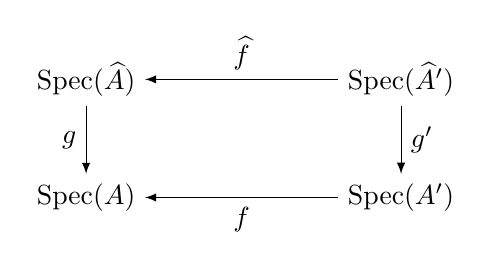
\begin{tikzpicture}[>=latex]
\node (tl) at (0,1.5) {$\operatorname{Spec}(\widehat A)$};
\node (tr) at (4,1.5) {$\operatorname{Spec}(\widehat{A}')$};
\node (bl) at (0,0) {$\operatorname{Spec}(A)$};
\node (br) at (4,0) {$\operatorname{Spec}(A')$};
\draw[->] (tr) -- node[above] {$\widehat f$} (tl);
\draw[->] (tl) -- node[left] {$g$} (bl);
\draw[->] (tr) -- node[right] {$g'$} (br);
\draw[->] (br) -- node[below] {$f$} (bl);
\end{tikzpicture}
\]
donde $g$ y $g'$ son los morfismos canónicos. Como, por hipótesis,
$f$ es un $\boldsymbol P$-morfismo y $g'$ es un morfismo regular,
de $(\mathrm P_{\mathrm I})$ se deduce que
$f\circ g'=g\circ\widehat f$ es un $\boldsymbol P$-morfismo.
Por otra parte, la hipótesis de que $f$ es un
$\boldsymbol P$-morfismo implica que $f$ es plano y, por tanto,
también lo es $\widehat f$ (Bourbaki, \emph{Alg. comm.},
cap. III, \S~5, n\textsuperscript{o}~4, cor. de la prop. 3);
el homomorfismo de anillos correspondiente es, además, local, por
lo que el morfismo es fielmente plano (\textbf 0$_{\mathrm I}$, 6.6.2).
De $(\mathrm P_{\mathrm{II}})$ se deduce entonces que $g$ es un
$\boldsymbol P$-morfismo.
\end{proof}

% END tree/worktree/es/DIPLOMATIC/EGA_IV2/ega4-2_7.4.2_ES.diplomatic.tex
% BEGIN tree/worktree/es/DIPLOMATIC/EGA_IV2/ega4-2_7.4.3_ES.diplomatic.tex
\begin{corollary}[7.4.3]
\label{IV.2.s7.4.3-fr}
\begin{enumerate}
\item[\emph{(i)}] Sea $A$ un $\boldsymbol P$-anillo local
noetheriano, y sea $A'=\widehat A$ su completado. Supongamos que,
para todo ideal primo $\mathfrak p'$ de $A'$, las fibras formales de
$A'_{\mathfrak p'}$ son geométricamente regulares; entonces, para
todo ideal primo $\mathfrak p$ de $A$, $A_{\mathfrak p}$ es un
$\boldsymbol P$-anillo.
\item[\emph{(ii)}] Supongamos que $\boldsymbol P$ satisface la
condición $(\mathrm P_{\mathrm{IV}})$ \textup{(7.3.6)}. Sean $A$ un
$\boldsymbol P$-anillo local noetheriano y $B$ una $A$-álgebra
local esencialmente de tipo finito, tal que el homomorfismo
$A\to B$ sea local. Pongamos $A'=\widehat A$, y sea
$\mathfrak n'$ el único ideal primo de $B'=B\otimes_A A'$ situado
sobre el ideal maximal de $B$ y el ideal maximal de $A'$. Si las
fibras formales de $B'_{\mathfrak n'}$ son geométricamente regulares,
entonces $B$ es un $\boldsymbol P$-anillo.
\end{enumerate}
\end{corollary}

\begin{proof}
\begin{enumerate}
\item[(i)] Como, por hipótesis,
$\operatorname{Spec}(A')\to\operatorname{Spec}(A)$ es un
$\boldsymbol P$-morfismo, también lo es
$\operatorname{Spec}(A'_{\mathfrak p'})\to
\operatorname{Spec}(A_{\mathfrak p})$ en virtud de (7.3.2, \emph{b)}),
para todo ideal primo $\mathfrak p$ de $A$ y todo ideal primo
$\mathfrak p'$ de $A'$ situado sobre $\mathfrak p$. Basta, pues,
aplicar el lema (7.4.2) a este morfismo, teniendo en cuenta que
$\operatorname{Spec}(A')\to\operatorname{Spec}(A)$ es sobreyectivo.
\item[(ii)] En virtud de (7.4.2), basta probar que el
morfismo
$\operatorname{Spec}(B'_{\mathfrak n'})\to\operatorname{Spec}(B)$
es un $\boldsymbol P$-morfismo. Ahora bien, se tiene
$B=C_{\mathfrak n}$, donde $C$ es una $A$-álgebra de tipo finito y
$\mathfrak n$ un ideal primo de $C$ situado sobre el ideal maximal
de $A$. Si se pone $C'=C\otimes_A A'$, de las hipótesis y de
(7.3.7) se deduce que
$\operatorname{Spec}(C')\to\operatorname{Spec}(C)$ es un
$\boldsymbol P$-morfismo; como $B'_{\mathfrak n'}$ es un anillo
local en un ideal primo de $C'$ situado sobre $\mathfrak n$, la
conclusión se deduce de (7.3.2, \emph{b)}).
\end{enumerate}
\end{proof}

% END tree/worktree/es/DIPLOMATIC/EGA_IV2/ega4-2_7.4.3_ES.diplomatic.tex
% BEGIN tree/worktree/es/DIPLOMATIC/EGA_IV2/ega4-2_7.4.4_statement_reduction_ES.diplomatic.tex
\begin{theorem}[7.4.4]
\label{IV.2.s7.4.4-fr}
Bajo las hipótesis sobre $\boldsymbol P$ de \textup{(7.4.1)}, sea $A$ un
$\boldsymbol P$-anillo local noetheriano.
\begin{enumerate}
\item[\emph{(i)}] Para todo ideal primo $\mathfrak p$ de $A$,
$A_{\mathfrak p}$ es un $\boldsymbol P$-anillo.
\item[\emph{(ii)}] Supongamos además que $\boldsymbol P$ satisface
la condición $(\mathrm P_{\mathrm{IV}})$. Entonces, todo anillo
local que sea una $A$-álgebra esencialmente de tipo finito es un
$\boldsymbol P$-anillo.
\end{enumerate}
\end{theorem}

\begin{proof}
\begin{enumerate}
\item[(i)] Aplicando (7.4.3, (i)), basta comprobar que,
para todo ideal primo $\mathfrak p'$ de $A'=\widehat A$,
$A'_{\mathfrak p'}$ tiene fibras formales geométricamente
regulares. Ahora bien, esto se demostró en (\textbf 0, 22.3.3 y 22.5.8).

\oldpage[IV-2]{200}

\item[(ii)] Sea $B$ una $A$-álgebra esencialmente de tipo
finito que sea un anillo local. Si $\mathfrak p$ es el ideal primo
de $A$ sobre el cual está situado el ideal maximal de $B$, $B$
también es una $A_{\mathfrak p}$-álgebra esencialmente de tipo
finito (1.3.8); en virtud de (i), se puede suponer, pues, que
$\mathfrak p$ es el ideal maximal $\mathfrak m$ de $A$. Entonces
$B=C_{\mathfrak q}$, donde $C$ es una $A$-álgebra de tipo finito y
$\mathfrak q$ un ideal primo de $C$ situado sobre $\mathfrak m$.
Sea $\mathfrak n\supset\mathfrak q$ un ideal maximal de $C$
(necesariamente situado sobre $\mathfrak m$). Si se pone
$k=A/\mathfrak m$, $C/\mathfrak mC$ es una $k$-álgebra de tipo
finito; por tanto, el cuerpo residual $k'$ de $C$ en el ideal
maximal $\mathfrak n$ es \emph{finito} sobre $k$ (\textbf I, 6.4.2). En virtud
de (i), bastará probar que $C_{\mathfrak n}$ es un
$\boldsymbol P$-anillo, puesto que $C_{\mathfrak q}$ es un anillo
local de $C_{\mathfrak n}$ en un ideal primo. La cuestión se reduce así
a demostrar el
\end{enumerate}
\end{proof}

% END tree/worktree/es/DIPLOMATIC/EGA_IV2/ega4-2_7.4.4_statement_reduction_ES.diplomatic.tex
% BEGIN tree/worktree/es/DIPLOMATIC/EGA_IV2/ega4-2_7.4.4.1_statement_ES.diplomatic.tex
\begin{lemma}[7.4.4.1]
\label{IV.2.s7.4.4.1-fr}
Sean $A$ un $\boldsymbol P$-anillo local noetheriano, $k$ su
cuerpo residual, $C$ una $A$-álgebra de tipo finito y $B$ un
anillo local en un ideal primo $\mathfrak n$ de $C$, tales que:
1\textsuperscript{o} el homomorfismo $A\to B$ es local;
2\textsuperscript{o} el cuerpo residual $k'$ de $B$ es una
extensión finita de $k$. Si $\boldsymbol P$ satisface
$(\mathrm P_{\mathrm{IV}})$, entonces $B$ es un
$\boldsymbol P$-anillo.
\end{lemma}

% END tree/worktree/es/DIPLOMATIC/EGA_IV2/ega4-2_7.4.4.1_statement_ES.diplomatic.tex
% BEGIN tree/worktree/es/DIPLOMATIC/EGA_IV2/ega4-2_7.4.4.1_proof_ES.diplomatic.tex
\begin{proof}
Sea $(x_i)_{1\leqslant i\leqslant m}$ un sistema de generadores de la
$A$-álgebra $C$; mostremos primero que se puede razonar por inducción sobre
$m$. Sea $C'$ la subálgebra de $C$ generada por
$x_1,\ldots,x_{m-1}$, y sea $\mathfrak n'=\mathfrak n\cap C'$.
El homomorfismo $A\to C_{\mathfrak n}$ se factoriza como
$A\to C'_{\mathfrak n'}\to C_{\mathfrak n}$, y está claro que
$A\to C'_{\mathfrak n'}$ y $C'_{\mathfrak n'}\to C_{\mathfrak n}$ son
homomorfismos locales; si $k''$ es el cuerpo residual de
$C'_{\mathfrak n'}$, $k\to k'$ se factoriza del mismo modo como
$k\to k''\to k'$, de modo que $k''$ es una extensión finita de $k$ y $k'$
una extensión finita de $k''$. La hipótesis de inducción implica que
$C'_{\mathfrak n'}$ es un $\boldsymbol P$-anillo; además, si
$S'=C'\setmin\mathfrak n'$, $C_{\mathfrak n}$ es un anillo local de
$S'^{-1}C$; como $C=C'[x_m]$, se tiene
$S'^{-1}C=C'_{\mathfrak n'}[x_m/1]$, y la hipótesis de inducción muestra
también que $C_{\mathfrak n}$ es un $\boldsymbol P$-anillo. La cuestión se reduce así al caso en que $C$ es una $A$-álgebra generada por \emph{un solo} elemento $t$.

Apliquemos (7.4.3, (ii)); poniendo $A'=\widehat A$,
$B'=B\otimes_A A'$ es un anillo local de $C\otimes_A A'$ en un ideal
primo situado sobre $\mathfrak n$; como $A$ y $A'$ tienen el mismo cuerpo
residual $k$, el cuerpo residual de $C\otimes_A A'$ en ese ideal primo es
igual a $k'$. Por otra parte, $C\otimes_A A'$ es una $A'$-álgebra generada
por un solo elemento. Resulta, pues, de (7.4.3, (ii)) que es posible
limitarse a demostrar (7.4.4.1) cuando $\boldsymbol P$ es la propiedad
(iv$'$) de (7.3.8), $A$ es \emph{completo} y $C$ está generada por un solo
elemento $t$.

Para demostrar entonces que las fibras formales de $B=C_{\mathfrak n}$
son geométricamente regulares, apliquemos el criterio (7.3.16, \emph{b)}). Sea
$B_1$ una $B$-álgebra finita e \emph{íntegra}, generada por tanto por un
número finito de elementos enteros sobre $B$. Multiplicando estos
elementos por un elemento de $S=C\setmin\mathfrak n$, se puede suponer que son
enteros sobre $C$ y, por consiguiente, escribir $B_1=S^{-1}C_1$, donde
$C_1$ es una sub-$C$-álgebra de $B_1$ generada por un número finito de
elementos enteros sobre $C$; es, por tanto, una $C$-álgebra
\emph{finita e íntegra}. Por otra parte, $B_1$ es un anillo semilocal, y
todo anillo local $B_2$ de $B_1$ en un ideal maximal es un anillo local
de $C_1$ en un ideal primo, tal que $A\to B_2$ es un homomorfismo local;
además, el cuerpo residual de $B_2$ es una extensión finita de $k'$ y,
por tanto, de $k$. Se ve así, teniendo en cuenta (7.3.14) y (i), que
el problema se reduce a la cuestión siguiente: sea $C$ un anillo noetheriano
\emph{íntegro}, que contiene un subanillo $C_0$ que es una $A$-álgebra
generada por un solo elemento $t$, y tal que $C$ es una $C_0$-álgebra
\emph{finita}; si $\mathfrak n$ es un ideal maximal de $C$
\oldpage[IV-2]{201}
situado sobre el ideal maximal de $A$, y $B=C_{\mathfrak n}$, se trata
de demostrar que, para todo ideal primo $\mathfrak q$ de $\widehat B$
cuya imagen inversa en $B$ sea 0, el anillo
$\widehat B_{\mathfrak q}$ es \emph{regular}. Por otra parte, se puede
sustituir $A$ por su imagen en $C$, que es un anillo local completo
(como cociente de $A$) e íntegro. La conclusión que hay que demostrar
es entonces consecuencia del lema siguiente, en apariencia más general:
\end{proof}

% END tree/worktree/es/DIPLOMATIC/EGA_IV2/ega4-2_7.4.4.1_proof_ES.diplomatic.tex
% BEGIN tree/worktree/es/DIPLOMATIC/EGA_IV2/ega4-2_7.4.4.2_statement_ES.diplomatic.tex
\begin{lemma}[7.4.4.2]
\label{IV.2.s7.4.4.2-fr}
Sean $A$ un anillo local noetheriano, íntegro y completo, $k$ su cuerpo
residual, y $C$ un anillo íntegro que contiene a $A$, tal que existe
$t\in C$ para el cual $C$ es una $A[t]$-álgebra finita. Sea $\mathfrak n$
un ideal maximal de $C$ situado sobre el ideal maximal $\mathfrak m$ de
$A$; pongamos $B=C_{\mathfrak n}$, $X=\operatorname{Spec}(B)$,
$B'=\widehat B$, $X'=\operatorname{Spec}(\widehat B)$; si
$U=\operatorname{Reg}(X)$, $U'=\operatorname{Reg}(X')$, y si
$f:X'\to X$ es el morfismo canónico, entonces
$f^{-1}(U)\subset U'$.
\end{lemma}

% END tree/worktree/es/DIPLOMATIC/EGA_IV2/ega4-2_7.4.4.2_statement_ES.diplomatic.tex
% BEGIN tree/worktree/es/DIPLOMATIC/EGA_IV2/ega4-2_7.4.4.2_proof_ES.diplomatic.tex
\begin{proof}
La afirmación que hay que demostrar para obtener (7.4.4.1) se deduce
de este lema observando que, puesto que $B$ es íntegro, el punto
genérico de $X$ pertenece a $U$.

Se observará que, como $C$ es una $A$-álgebra de tipo finito y $\mathfrak n$
un ideal maximal de $C$, el cuerpo residual $k'$ de
$C_{\mathfrak n}=B$ (y, por tanto, también de $B'$) es una extensión
\emph{finita} de $k$ (\textbf I, 6.4.11 y 6.4.2).

Si se pone $Y=\operatorname{Spec}(C)$, de (6.12.8) resulta que
$\operatorname{Reg}(Y)$ es \emph{abierto} en $Y$; como los anillos locales de
$X$ son anillos locales de $Y$ (\textbf I, 2.4.2), se tiene
$U=X\cap\operatorname{Reg}(Y)$, y por tanto $U$ es \emph{abierto} en $X$; por
otra parte, según (6.12.7), $U'$ es abierto en $X'$, de modo que
$S'=X'\setmin U'$ es cerrado. En consecuencia, $S'\cap f^{-1}(U)$ es
\emph{localmente cerrado} en $X'$, y basta demostrar que este conjunto es
\emph{vacío}. Se sabe por (5.1.10) que, en caso contrario, existiría en
$S'\cap f^{-1}(U)$ un ideal primo $\mathfrak p'$ tal que
$\dim(B'/\mathfrak p')\leqslant1$. Observemos primero que
$\mathfrak p'$ no puede ser el ideal maximal $\mathfrak mB'$ de $B'$,
donde $\mathfrak m$ es el ideal maximal de $B$. En efecto, esto
significaría que $B=B_{\mathfrak m}$ sería regular, y por tanto también
$B'=\widehat B$ (\textbf{0}, 17.1.5); se tendría entonces $\mathfrak mB'\in U'$,
en contra de la hipótesis. Debe ser, pues,
$\dim(B'/\mathfrak p')=1$. Pongamos
$\mathfrak p=B\cap\mathfrak p'$; por hipótesis, $B_{\mathfrak p}$ es
regular, pero $B'_{\mathfrak p'}$ no lo es; como
$B'_{\mathfrak p'}$ es un $B_{\mathfrak p}$-módulo plano, se deduce de
(6.5.2) que la fibra $Z$ de $f$ en el punto $\mathfrak p$ \emph{no es regular
en el punto} $\mathfrak p'$. Mostremos que \emph{es posible reducirse al caso en
que} $\mathfrak p=0$. En efecto, en el caso general, si se pone
$\mathfrak q=\mathfrak p\cap C$, $\mathfrak r=\mathfrak p\cap A$,
$C/\mathfrak q$ es una $(A/\mathfrak r)[\bar t]$-álgebra finita (donde
$\bar t$ es la clase de $t$ módulo $\mathfrak q$); como
$\mathfrak p=\mathfrak qB$, $B/\mathfrak p$ es igual a
$(C/\mathfrak q)_{\mathfrak n/\mathfrak q}$, y
$\mathfrak n/\mathfrak q$ es un ideal maximal de $C/\mathfrak q$
situado sobre el ideal maximal $\mathfrak m/\mathfrak r$ de
$A/\mathfrak r$. Se ve así que $A/\mathfrak r$, $C/\mathfrak q$ y
$B/\mathfrak p$ siguen satisfaciendo las hipótesis de (7.4.4.2); como
el completado de $B/\mathfrak p$ es $B'/\mathfrak pB'$, esto demuestra
nuestra afirmación. Supongamos, pues, $\mathfrak p=0$, de manera que
$Z$ es la fibra genérica y el homomorfismo $B\to B'/\mathfrak p'$ es
\emph{inyectivo}. Pongamos $V=B'/\mathfrak p'$ y distingamos dos casos:

I) \emph{$V$ es una $A$-álgebra finita.} --- Como $B\subset V$, $B$ es
\emph{a fortiori} una $A$-álgebra finita; y, puesto que $A$ es completo,
lo mismo ocurre con $B$ (Bourbaki, \emph{Alg. comm.}, cap. IV, \S~2,
n\textsuperscript{o}~5, cor. 3 de la prop. 9). De ahí que $B'=B$ y
$\mathfrak p'=0$, por lo que $B'_{\mathfrak p'}$ es un cuerpo y, por
consiguiente, un anillo regular, en contra de la hipótesis.

II) \emph{$V$ no es una $A$-álgebra finita.} --- Como el anillo local
$A$ es \emph{completo}, esto implica que $V$ no es una $A$-álgebra
\emph{cuasifinita} ($\mathbf{0}_{\mathrm I}$, 7.4.1 y 7.4.2); pero, por hipótesis, el
cuerpo residual $k'$ de $V$ es una extensión \emph{finita} del cuerpo residual
$k$ de $A$,
\oldpage[IV-2]{202}
por tanto, según ($\mathbf{0}_{\mathrm I}$, 7.4.4), el ideal $\mathfrak mV$
\emph{no es un ideal de definición de} $V$. Como $V$ es un anillo local noetheriano
íntegro de dimensión 1, 0 es el único ideal de $V$ que no es un ideal
de definición; por ello, $\mathfrak mV=0$. Pero $A\subset V$ y $V$ es
íntegro, de donde $\mathfrak m=0$ y $A=k$ es un \emph{cuerpo}. Se deduce ante
todo que $\dim(C)\leqslant1$ (\textbf 0, 16.1.5); pero, como $\dim(V)=1$, las
relaciones
$\dim(V)\leqslant\dim(B')=\dim(B)\leqslant\dim(C)$
muestran que esto implica
$\dim(C)=\dim(B)=\dim(B')=\dim(B'/\mathfrak p')=1$ y, en consecuencia,
$\mathfrak p'$ es necesariamente un \emph{ideal primo minimal} de $B'$.
Llegaremos, pues, también a una contradicción si demostramos que
$B'_{\mathfrak p'}$ es un \emph{cuerpo}, o, lo que es lo mismo, que el anillo
$B'$ es reducido. Ahora bien, como $C$ es una $k$-álgebra de tipo finito,
la clausura integral $C_1$ de $C$ es una $C$-álgebra \emph{finita} (Bourbaki,
\emph{Alg. comm.}, cap. V, \S~3, n\textsuperscript{o}~2, teorema 2);
si se pone $S=C\setmin\mathfrak n$, $B_1=S^{-1}C_1$ es la clausura integral de
$B$, y por tanto $B_1$ es una $B$-álgebra \emph{finita}, y en consecuencia es
un anillo semilocal noetheriano, íntegro, integralmente cerrado y de
dimensión 1 (\textbf{0}, 16.1.5). Si $\mathfrak m_j$ $(1\leqslant j\leqslant h)$
son sus ideales maximales, los $(B_1)_{\mathfrak m_j}$ son, por tanto,
anillos de valoración discreta (\textbf{II}, 7.1.6), y el completado $B'_1$ de
$B_1$ es el producto directo de los anillos de valoración discreta
completados de los $(B_1)_{\mathfrak m_j}$ (Bourbaki, \emph{Alg. comm.},
cap. III, \S~2, n\textsuperscript{o}~13, prop. 18); $B'_1$ es, pues,
reducido, y como el completado $B'$ de $B$ es un subanillo de $B'_1$
(Bourbaki, \emph{Alg. comm.}, cap. IV, \S~2, n\textsuperscript{o}~5,
cor. 3 de la prop. 9), también es un anillo reducido. Queda demostrado.
\end{proof}

% END tree/worktree/es/DIPLOMATIC/EGA_IV2/ega4-2_7.4.4.2_proof_ES.diplomatic.tex
% BEGIN tree/worktree/es/DIPLOMATIC/EGA_IV2/ega4-2_7.4.5_ES.diplomatic.tex
\begin{corollary}[7.4.5]
\label{IV.2.s7.4.5-fr}
Supongamos que la propiedad $\boldsymbol P$ satisface las condiciones
$(\mathrm P_{\mathrm I})$, $(\mathrm P_{\mathrm{II}})$ y
$(\mathrm P_{\mathrm{III}})$. Sea $A$ un anillo noetheriano. Las
condiciones siguientes son equivalentes:
\begin{enumerate}
\item[\emph{a)}] Para todo ideal primo $\mathfrak p$ de $A$,
$A_{\mathfrak p}$ es un $\boldsymbol P$-anillo.
\item[\emph{b)}] Para todo ideal maximal $\mathfrak m$ de $A$,
$A_{\mathfrak m}$ es un $\boldsymbol P$-anillo.
\end{enumerate}
Si además $\boldsymbol P$ satisface $(\mathrm P_{\mathrm{IV}})$, las
propiedades \textup{a)} y \textup{b)} son también equivalentes a:
\begin{enumerate}
\item[\emph{c)}] Para toda $A$-álgebra de tipo finito $B$ y todo ideal
primo $\mathfrak q$ de $B$, $B_{\mathfrak q}$ es un
$\boldsymbol P$-anillo.
\end{enumerate}
\end{corollary}

\begin{proof}
La equivalencia de \emph{a)} y \emph{b)} resulta de (7.4.4, (i)), y la de \emph{a)} y \emph{c)} de
(7.4.4, (ii)).

Cuando se cumple la condición \emph{a)} de (7.4.5), se dice que $A$ es un
$\boldsymbol P$-\emph{anillo}; para los anillos semilocales noetherianos, esta
definición coincide con la de (7.3.13) cuando se satisfacen las
condiciones $(\mathrm P_{\mathrm I})$, $(\mathrm P_{\mathrm{II}})$ y
$(\mathrm P_{\mathrm{III}})$. El anillo $\mathbf Z$ es un
$\boldsymbol P$-anillo (7.3.19, (iv)); todo anillo local completo es un
$\boldsymbol P$-anillo.
\end{proof}

% END tree/worktree/es/DIPLOMATIC/EGA_IV2/ega4-2_7.4.5_ES.diplomatic.tex
% BEGIN tree/worktree/es/DIPLOMATIC/EGA_IV2/ega4-2_7.4.6_ES.diplomatic.tex
\begin{proposition}[7.4.6]
\label{IV.2.s7.4.6-fr}
Supongamos que la propiedad $\boldsymbol P$ satisface las condiciones
$(\mathrm P_{\mathrm I})$, $(\mathrm P_{\mathrm{II}})$ y
$(\mathrm P_{\mathrm{III}})$. Sean $A$ un anillo noetheriano,
$\mathfrak J$ un ideal de $A$ y $\widehat A$ el completado separado de
$A$ para la topología $\mathfrak J$-preádica. Entonces, si $A$ es un
$\boldsymbol P$-anillo (7.4.5), el morfismo canónico
$\operatorname{Spec}(\widehat A)\to\operatorname{Spec}(A)$ es un
$\boldsymbol P$-morfismo.
\end{proposition}

\begin{proof}
Utilizando (7.3.2, \emph{c$'$)}), basta demostrar que, para todo ideal
maximal $\mathfrak n$ de $\widehat A$ cuya imagen inversa es
$\mathfrak m$ en $A$, el morfismo
$\operatorname{Spec}((\widehat A)_{\mathfrak n})\to
\operatorname{Spec}(A_{\mathfrak m})$ es un $\boldsymbol P$-morfismo.
Se sabe (Bourbaki, \emph{Alg. comm.}, cap. III, \S~3,
n\textsuperscript{o}~4, prop. 8) que el homomorfismo canónico
$A_{\mathfrak m}\to(\widehat A)_{\mathfrak n}$ es inyectivo, que la
topología $\mathfrak mA_{\mathfrak m}$-preádica sobre $A_{\mathfrak m}$
está inducida por la topología
$\mathfrak n(\widehat A)_{\mathfrak n}$-preádica y que
$A_{\mathfrak m}$ es denso en $(\widehat A)_{\mathfrak n}$ para esta
topología; por consiguiente, el completado de $A_{\mathfrak m}$ para la
topología $\mathfrak mA_{\mathfrak m}$-preádica se identifica con el de
$(\widehat A)_{\mathfrak n}$ para la topología
$\mathfrak n(\widehat A)_{\mathfrak n}$-preádica. Se tienen, pues, dos
morfismos
\[
\operatorname{Spec}((A_{\mathfrak m})^{\widehat{\,}})
\xrightarrow{f}\operatorname{Spec}((\widehat A)_{\mathfrak n})
\xrightarrow{g}\operatorname{Spec}(A_{\mathfrak m})
\]

\oldpage[IV-2]{203}

tales que $f$ es fielmente plano; como, por hipótesis, $g\circ f$ es un
$\boldsymbol P$-morfismo, también lo es $g$ en virtud de
$(\mathrm P_{\mathrm{II}})$.
\end{proof}

% END tree/worktree/es/DIPLOMATIC/EGA_IV2/ega4-2_7.4.6_ES.diplomatic.tex
% BEGIN tree/worktree/es/DIPLOMATIC/EGA_IV2/ega4-2_7.4.7_ES.diplomatic.tex
\begin{corollary}[7.4.7]
\label{IV.2.s7.4.7-fr}
Supongamos que $\boldsymbol P$ satisface las condiciones
$(\mathrm P_{\mathrm I})$, $(\mathrm P'_{\mathrm I})$,
$(\mathrm P_{\mathrm{II}})$, $(\mathrm P_{\mathrm{III}})$ y
$(\mathrm P_{\mathrm{IV}})$. Entonces, si $A$ es un
$\boldsymbol P$-anillo (7.4.5), el morfismo canónico
$\operatorname{Spec}(A[[T_1,\ldots,T_r]])\to\operatorname{Spec}(A)$ es un
$\boldsymbol P$-morfismo. En particular, si además $A$ es íntegro, $K$
su cuerpo de fracciones, y si $\mathfrak p$ es un ideal primo de
$B=A[[T_1,\ldots,T_r]]$ tal que $\mathfrak p\cap A=0$, entonces se
cumple la propiedad $\boldsymbol P(B_{\mathfrak p},K)$.
\end{corollary}

\begin{proof}
En efecto, el morfismo canónico
$\operatorname{Spec}(B)\to\operatorname{Spec}(A)$ se factoriza como
\[
\operatorname{Spec}(A[[T_1,\ldots,T_r]])
\xrightarrow{f}\operatorname{Spec}(A[T_1,\ldots,T_r])
\xrightarrow{g}\operatorname{Spec}(A).
\]
Está claro que el morfismo $g$ es regular (\textbf 0, 17.3.7); en virtud de
(7.4.5), $A[T_1,\ldots,T_r]$ es un $\boldsymbol P$-anillo, de modo que
por (7.4.6) $f$ es un $\boldsymbol P$-morfismo. Como $g$ es regular y,
por tanto, también un $\boldsymbol P$-morfismo (7.3.5, (i)), lo mismo
vale para $g\circ f$ en virtud de $(\mathrm P'_{\mathrm I})$.

Se observará que la conclusión sigue siendo válida si, en lugar de suponer
que $\boldsymbol P$ satisface $(\mathrm P'_{\mathrm I})$ y que todo
morfismo regular es un $\boldsymbol P$-morfismo, se supone únicamente
que un morfismo compuesto $g\circ f$ es un $\boldsymbol P$-morfismo
cuando $g$ es regular y $f$ un $\boldsymbol P$-morfismo (condición en
cierto modo simétrica de $(\mathrm P'_{\mathrm I})$).
\end{proof}

% END tree/worktree/es/DIPLOMATIC/EGA_IV2/ega4-2_7.4.7_ES.diplomatic.tex
% BEGIN tree/worktree/es/DIPLOMATIC/EGA_IV2/ega4-2_7.4.8_ES.diplomatic.tex
\begin{remark}[7.4.8]
\label{IV.2.s7.4.8-fr}
Los resultados anteriores plantean los problemas siguientes:
\begin{enumerate}
\item[A)] Sea $A$ un anillo de Zariski \emph{completo}, y sea
$\mathfrak J$ un ideal de definición de $A$; si el anillo
$A/\mathfrak J$ es un $\boldsymbol P$-anillo, ¿lo es también $A$? De
ello resultaría que, para todo $\boldsymbol P$-anillo noetheriano $A$ y
todo ideal $\mathfrak J$ de $A$, el completado separado $\widehat A$
para la topología $\mathfrak J$-preádica sería también un
$\boldsymbol P$-anillo.
\item[B)] Sea $k$ un cuerpo valuado completo no discreto; se
llama también anillo de \emph{series formales restringidas}
$k\{T_1,\ldots,T_n\}$ al subanillo del anillo de series formales
$k[[T_1,\ldots,T_n]]$ formado por las series cuyos coeficientes
\emph{tienden a} 0. ¿Es tal anillo un $\boldsymbol P$-anillo?
\item[C)] Si $A$ es un $\boldsymbol P$-anillo linealmente
topologizado y $S$ un conjunto multiplicativo de $A$, ¿son los anillos
$A\{S^{-1}\}$ ($\mathbf{0}_{\mathrm I}$, 7.6.1) y $A_{\{S\}}$
($\mathbf{0}_{\mathrm I}$, 7.6.15) $\boldsymbol P$-anillos?
\end{enumerate}
\end{remark}

% END tree/worktree/es/DIPLOMATIC/EGA_IV2/ega4-2_7.4.8_ES.diplomatic.tex
% BEGIN tree/worktree/es/DIPLOMATIC/EGA_IV2/ega4-2_7.5.0_ES.diplomatic.tex
\subsection{Un criterio para los $\boldsymbol P$-morfismos.}
\label{subsection:IV.7.5-fr}

\begin{env}[7.5.0]
\label{IV.2.s7.5.0-fr}
Este apartado no se utilizará en el resto del capítulo IV y, por tanto,
puede omitirse en una primera lectura. Veremos además más adelante
(7.9.8) que los resultados de este apartado pueden mejorarse
considerablemente cuando se dispone de la «resolución de
singularidades».

En lo que sigue de este apartado consideraremos una propiedad
$\boldsymbol R(A)$ y denotaremos por $\boldsymbol P(Z,k)$ la propiedad
siguiente:
\begin{quote}
«$Z$ es un preesquema localmente noetheriano sobre un cuerpo $k$ y, para
toda extensión \emph{finita} $k'$ de $k$, si se pone $Z'=Z\otimes_k k'$, se
cumple la propiedad $\boldsymbol R(\mathscr O_{Z',z'})$ para todo
$z'\in Z'$.»
\end{quote}
\end{env}

% END tree/worktree/es/DIPLOMATIC/EGA_IV2/ega4-2_7.5.0_ES.diplomatic.tex
% BEGIN tree/worktree/es/DIPLOMATIC/EGA_IV2/ega4-2_7.5.1_statement_ES.diplomatic.tex
\begin{theorem}[7.5.1]
\label{IV.2.s7.5.1-fr}
Sean $A$, $B$ dos anillos locales noetherianos \textup{completos}, $\mathfrak m$
el ideal maximal de $A$, $k=A/\mathfrak m$ su cuerpo residual y
$\varphi:A\to B$ un homomorfismo local tal que:
\begin{enumerate}
\item[\emph{(i)}] El cuerpo residual de $B$ es una extensión finita de
$k$.
\item[\emph{(ii)}] $B$ es un $A$-módulo plano.
\end{enumerate}
Sea, por otra parte, $\boldsymbol R(C)$ una propiedad que satisface la
condición $(\mathrm R_{\mathrm{III}})$ (7.3.18) y la condición siguiente:
\begin{quote}
$(\mathrm R_{\mathrm{IV}})$ Para todo anillo local $C$ en un ideal primo
de un anillo local noetheriano completo y todo elemento $C$-regular $t$
del ideal maximal de $C$, la propiedad $\boldsymbol R(C/tC)$ implica
$\boldsymbol R(C)$.
\end{quote}

\oldpage[IV-2]{204}

En estas condiciones, sea $f={}^a\varphi:\operatorname{Spec}(B)\to
\operatorname{Spec}(A)$, y supongamos que se cumple la propiedad
$\boldsymbol P(\operatorname{Spec}(B\otimes_A k),k)$. Entonces, para
todo $x\in\operatorname{Spec}(A)$ se cumple la propiedad
$\boldsymbol P(f^{-1}(x),\boldsymbol{k}(x))$.
\end{theorem}

% END tree/worktree/es/DIPLOMATIC/EGA_IV2/ega4-2_7.5.1_statement_ES.diplomatic.tex
% BEGIN tree/worktree/es/DIPLOMATIC/EGA_IV2/ega4-2_7.5.1_proof_stage_I_ES.diplomatic.tex
\begin{proof}
En otras palabras, la propiedad $\boldsymbol P$ para \emph{la fibra del punto
cerrado} de $\operatorname{Spec}(A)$ implica la misma propiedad para
\emph{todas las fibras} del morfismo $f$ (es decir, que $f$ es un
$\boldsymbol P$-\emph{morfismo} (7.3.1)).

Procederemos en varias etapas:

I) \emph{Reducción al estudio de los anillos locales de la fibra
genérica.} --- Apliquemos el lema (7.3.16.2): basta comprobar que, para
toda $A$-álgebra \emph{finita} e \emph{íntegra} $A'$ con cuerpo de fracciones $K'$, si
se pone $B'=B\otimes_A A'$, todos los anillos locales de
$\operatorname{Spec}(B'\otimes_{A'}K')$ satisfacen la propiedad
$\boldsymbol R$. El anillo $A'$ (resp. $B'$) es semilocal
completo ($B'$ es una $B$-álgebra finita), y por tanto producto de
anillos locales completos; como $A'$ es íntegro por hipótesis, es \emph{local};
todo ideal maximal $\mathfrak n'$ de $B'$ está situado sobre el ideal
maximal $\mathfrak n$ de $B$ y, por tanto, sobre $\mathfrak m$; en
consecuencia, su imagen inversa en $A'$ es el ideal maximal
$\mathfrak m'$ de $A'$. Como todo anillo local de
$\operatorname{Spec}(B'\otimes_{A'}K')$ es un anillo local de
$\operatorname{Spec}(B')$, y por tanto de uno de los
$\operatorname{Spec}(B'_{\mathfrak n'})$ (sobre el punto genérico de
$A'$), se ve que bastará demostrar que los anillos locales de
$\operatorname{Spec}(B'_{\mathfrak n'}\otimes_{A'}K')$
poseen la propiedad $\boldsymbol R$. Ahora bien, $A'$ y
$B'_{\mathfrak n'}$ son anillos locales noetherianos completos; el
cuerpo residual de $B'_{\mathfrak n'}$ es una extensión finita del de
$B$, y por tanto también de $k$ y, \emph{a fortiori}, del cuerpo
residual $k'$ de $A'$. Esta observación y (2.1.4) muestran que $A'$ y
$B'_{\mathfrak n'}$ satisfacen las condiciones (i) y (ii) del
enunciado. Por otra parte, si $k''$ es una extensión finita de $k'$,
$k''$ es también una extensión finita de $k$, y los anillos locales de
$\operatorname{Spec}(B'_{\mathfrak n'}\otimes_{A'}k'')$
son también anillos locales de $\operatorname{Spec}(B\otimes_A k'')$;
por ello, la hipótesis de que se cumple
$\boldsymbol P(\operatorname{Spec}(B\otimes_A k),k)$ implica que la
propiedad
$\boldsymbol P(\operatorname{Spec}(B'_{\mathfrak n'}\otimes_{A'}k'),k')$
se cumple.

La cuestión se reduce así al caso en que, además, $A$ es \emph{íntegro}, con
cuerpo de fracciones $K$, y a demostrar que \emph{los anillos locales de}
$\operatorname{Spec}(B\otimes_A K)$ \emph{poseen la propiedad} $\boldsymbol R$.

% END tree/worktree/es/DIPLOMATIC/EGA_IV2/ega4-2_7.5.1_proof_stage_I_ES.diplomatic.tex
% BEGIN tree/worktree/es/DIPLOMATIC/EGA_IV2/ega4-2_7.5.1_proof_stage_II_ES.diplomatic.tex
II) \emph{Caso en que $\dim(A)=1$.} --- Sea $A'$ la clausura integral de
$A$; se sabe por (\textbf 0, 23.1.6) que $A'$ es una $A$-álgebra \emph{finita} y un
anillo \emph{local} completo. Si se pone $B'=B\otimes_A A'$, se tiene
$B\otimes_A K=B'\otimes_{A'}K$. El mismo razonamiento que en I) muestra
que, para todo ideal maximal $\mathfrak n'$ de $B'$, basta demostrar que
los anillos locales de $B'_{\mathfrak n'}\otimes_{A'}K$ satisfacen
$\boldsymbol R$; además, ese razonamiento muestra también que $A'$ y
$B'_{\mathfrak n'}$ satisfacen las hipótesis (i) y (ii) del enunciado y
que se cumple
$\boldsymbol P(\operatorname{Spec}(B'_{\mathfrak n'}\otimes_{A'}k'),k')$
(donde $k'$ es el cuerpo residual de $A'$). Además, como
$\dim(A')=1$ (\textbf 0, 16.1.5) y $A'$ es íntegro e integralmente cerrado,
es un \emph{anillo de valoración discreta completo}. Es posible, pues,
limitarse al caso en que $A$ ya es un anillo de valoración discreta
completo. Si $u$ es entonces un generador del ideal maximal de $A$,
el hecho de que $u$ sea $A$-regular y de que $B$ sea un $A$-módulo
plano implica que $t=\varphi(u)$ es un elemento $B$-regular que
pertenece al ideal maximal de $B$. La hipótesis de que se cumple
$\boldsymbol P(\operatorname{Spec}(B\otimes_A k),k)$ implica, en
particular, que se cumple $\boldsymbol R(B/tB)$; en virtud de
$(\mathrm R_{\mathrm{IV}})$, se cumple, por tanto, $\boldsymbol R(B)$.
En otras palabras, $U_{\mathbf R}(\operatorname{Spec}(B))$ contiene
el punto cerrado de $\operatorname{Spec}(B)$. Pero
$U_{\mathbf R}(\operatorname{Spec}(B))$ es abierto en virtud de
$(\mathrm R_{\mathrm{III}})$, y $\operatorname{Spec}(B)$ es el único
abierto de $\operatorname{Spec}(B)$ que contiene el punto cerrado.
Por ello, todos los anillos locales de $\operatorname{Spec}(B)$ poseen
la propiedad $\boldsymbol R$, en particular los de
$\operatorname{Spec}(B\otimes_A K)$.

% END tree/worktree/es/DIPLOMATIC/EGA_IV2/ega4-2_7.5.1_proof_stage_II_ES.diplomatic.tex
% BEGIN tree/worktree/es/DIPLOMATIC/EGA_IV2/ega4-2_7.5.1_proof_stage_III_ES.diplomatic.tex
III) \emph{Caso general.} --- El caso $\dim(A)=0$ es trivial, pues entonces
$A=k$; es posible, por tanto, limitarse al caso en que $\dim(A)\geqslant1$.
Se sabe (6.12.7) que $\operatorname{Spec}(A)$ contiene un abierto no vacío
$V$ cuyos puntos son todos regulares; como $\dim(A)\geqslant1$, la
intersección $V'$ de $V$ con el complementario del punto cerrado de
$\operatorname{Spec}(A)$ es un abierto no vacío y contiene, por tanto, el
punto genérico de $\operatorname{Spec}(A)$. Si demostramos que
$f^{-1}(V')\subset U_{\mathbf R}(\operatorname{Spec}(B))$,
la proposición quedará demostrada \emph{a fortiori}. En otras palabras,
basta ver que el conjunto $Z$, intersección de $f^{-1}(V')$ con el
complementario de $U_{\mathbf R}(\operatorname{Spec}(B))$, es \emph{vacío}.
Razonemos por contradicción: como, en virtud de
$(\mathrm R_{\mathrm{III}})$,
$U_{\mathbf R}(\operatorname{Spec}(B))$ es abierto en
$\operatorname{Spec}(B)$, $Z$ es localmente cerrado en
$\operatorname{Spec}(B)$; si no fuera vacío, contendría un punto $x$ tal
que $\dim(\overline{\{x\}})\leqslant1$ (5.1.10); como $f(x)\in V'$
es distinto del punto cerrado de $\operatorname{Spec}(A)$, $x$ es distinto
del punto cerrado de $\operatorname{Spec}(B)$, es decir,
$\dim(\overline{\{x\}})=1$. Vamos a demostrar que esto es imposible,
es decir, que, si $\dim(\overline{\{x\}})=1$ y $f(x)\in V'$, se cumple
$\boldsymbol R(\mathscr O_x)$. Dicho de otro modo, se trata de ver que,
si $\mathfrak q$ es un ideal primo de $B$ tal que
$\dim(B/\mathfrak q)=1$ y si $\mathfrak p=\varphi^{-1}(\mathfrak q)$
es distinto de $\mathfrak m$ y tal que $A_{\mathfrak p}$ es \emph{regular},
entonces se cumple $\boldsymbol R(B_{\mathfrak q})$. Como
$\mathfrak p\ne\mathfrak m$, $\mathfrak m(B/\mathfrak q)$ no se reduce
a 0 y, por tanto, es un ideal de definición del anillo local íntegro
$B/\mathfrak q$ de dimensión 1; por otra parte, en virtud de (i), el
cuerpo residual de $B/\mathfrak q$ es una extensión finita del cuerpo
residual $k$ de $A/\mathfrak p$, por lo que $B/\mathfrak q$ es una
$(A/\mathfrak p)$-álgebra \emph{cuasifinita} ($\mathbf{0}_{\mathrm I}$, 7.4.4). Pero
$A/\mathfrak p$ es completo y $B/\mathfrak q$ es separado para la
topología $\mathfrak m$-preádica (que coincide con su topología de anillo
local); por tanto ($\mathbf{0}_{\mathrm I}$, 7.4.1), $B/\mathfrak q$ es una
$(A/\mathfrak p)$-álgebra \emph{finita}. Además, por definición, el homomorfismo
$A/\mathfrak p\to B/\mathfrak q$ es inyectivo, por lo que (\textbf{0}, 16.1.5)
se tiene
$\dim(A/\mathfrak p)=\dim(B/\mathfrak q)=1$.
Se puede entonces aplicar a los anillos $A/\mathfrak p$ y
$B/\mathfrak pB$ el resultado de II), pues los cuerpos residuales de
estos anillos locales son, respectivamente, los de $A$ y $B$, y
$B/\mathfrak pB$ es un $(A/\mathfrak p)$-módulo plano; además, se tiene
$(B/\mathfrak pB)\otimes_{A/\mathfrak p}k=B\otimes_A k=B/\mathfrak mB$.
Por consiguiente, los anillos locales de
$\operatorname{Spec}((B/\mathfrak pB)
\otimes_{A/\mathfrak p}\boldsymbol{k}(\mathfrak p))$
satisfacen $\boldsymbol R$. Ahora bien,
$B_{\mathfrak q}/\mathfrak pB_{\mathfrak q}$ es uno de los anillos
locales de $\operatorname{Spec}((B/\mathfrak pB)
\otimes_{A/\mathfrak p}\boldsymbol{k}(\mathfrak p))$. Además, $B_{\mathfrak q}$ es
un $A_{\mathfrak p}$-módulo plano y $A_{\mathfrak p}$ es \emph{regular}.
Se tiene, pues, el siguiente lema:

% END tree/worktree/es/DIPLOMATIC/EGA_IV2/ega4-2_7.5.1_proof_stage_III_ES.diplomatic.tex
% BEGIN tree/worktree/es/DIPLOMATIC/EGA_IV2/ega4-2_7.5.1.1_statement_ES.diplomatic.tex
\oldpage[IV-2]{205}

\begin{lemma}[7.5.1.1]
\label{IV.2.s7.5.1.1-fr}
Sea $\boldsymbol{C}$ una subcategoría plena de la categoría de los anillos
locales noetherianos, tal que todo anillo cociente de un anillo de
$\boldsymbol{C}$ pertenezca también a $\boldsymbol{C}$. Sea $\boldsymbol R(C)$
una propiedad tal que, si $C\in\boldsymbol{C}$ y $t$ es un elemento regular
del ideal maximal de $C$ para el que se cumple $\boldsymbol R(C/tC)$,
entonces se cumple $\boldsymbol R(C)$.

En estas condiciones, sean $C$ un anillo local regular, $k$ su cuerpo
residual, $D$ un anillo local que pertenece a $\boldsymbol{C}$, y
$\varphi:C\to D$ un homomorfismo local que hace de $D$ un $C$-módulo
plano. Si se cumple $\boldsymbol R(D\otimes_C k)$, entonces también
se cumple $\boldsymbol R(D)$.
\end{lemma}

% END tree/worktree/es/DIPLOMATIC/EGA_IV2/ega4-2_7.5.1.1_statement_ES.diplomatic.tex
% BEGIN tree/worktree/es/DIPLOMATIC/EGA_IV2/ega4-2_7.5.1.1_proof_ES.diplomatic.tex
\begin{proof}
Razonemos por inducción sobre $n=\dim(C)$. El lema es cierto por hipótesis
si $n=0$, pues entonces $C=k$. Sea $t$ un elemento del ideal maximal
$\mathfrak m$ de $C$ que no pertenece a $\mathfrak m^2$; se sabe entonces que
$C/tC$ es regular y que $\dim(C/tC)=n-1$ ((\textbf 0, 17.1.8) y (\textbf 0, 16.3.4)).
Como
$(D/tD)\otimes_{C/tC}k=D\otimes_C k$,
y $D/tD\in\boldsymbol{C}$, la hipótesis de inducción muestra que se cumple
$\boldsymbol R(D/tD)$; además, $t$ es $C$-regular y, por planitud,
también $D$-regular (\textbf 0$_{\mathrm I}$, 6.3.4). La hipótesis sobre
$\boldsymbol R$ muestra, por tanto, que se cumple $\boldsymbol R(D)$.
\end{proof}

% END tree/worktree/es/DIPLOMATIC/EGA_IV2/ega4-2_7.5.1.1_proof_ES.diplomatic.tex
% BEGIN tree/worktree/es/DIPLOMATIC/EGA_IV2/ega4-2_7.5.1_proof_conclusion_ES.diplomatic.tex
Para terminar la demostración de (7.5.1), basta aplicar aquí el lema
(7.5.1.1) tomando como $\boldsymbol{C}$ la categoría de los anillos locales
de los espectros de anillos locales completos, teniendo en cuenta la
hipótesis $(\mathrm R_{\mathrm{IV}})$, y tomando como $C$ el anillo
$A_{\mathfrak p}$ y como $D$ el anillo $B_{\mathfrak q}$.
\end{proof}

% END tree/worktree/es/DIPLOMATIC/EGA_IV2/ega4-2_7.5.1_proof_conclusion_ES.diplomatic.tex
% BEGIN tree/worktree/es/DIPLOMATIC/EGA_IV2/ega4-2_7.5.2_ES.diplomatic.tex
\begin{corollary}[7.5.2]
\label{IV.2.s7.5.2-fr}
Sean $A$ un anillo local noetheriano, $\mathfrak m$ el ideal maximal de $A$,
$k=A/\mathfrak m$ su cuerpo residual, $B$ un anillo local noetheriano
y $\varphi:A\to B$ un homomorfismo local tal que:
\begin{enumerate}
\item[\emph{(i)}] El cuerpo residual de $B$ es una extensión finita de $k$.
\item[\emph{(ii)}] $B$ es un $A$-módulo plano.
\end{enumerate}
Sea, por otra parte, $\boldsymbol R(C)$ una propiedad que satisface las
condiciones $(\mathrm R_{\mathrm{II}})$ \textup{(7.3.10)},
$(\mathrm R_{\mathrm{III}})$ \textup{(7.3.18)} y $(\mathrm R_{\mathrm{IV}})$
\textup{(7.5.1)}. Por último, sea $\boldsymbol R'(C)$ una propiedad que satisface
la condición siguiente:
\begin{quote}
$(\mathrm R_{\mathrm V})$ Si $C$ y $D$ son dos anillos locales
noetherianos y $\psi:C\to D$ es un homomorfismo local tal que
\[
g={}^a\psi:\operatorname{Spec}(D)\to\operatorname{Spec}(C)
\]
es un $\boldsymbol P$-morfismo, entonces la propiedad
$\boldsymbol R'(C)$ implica $\boldsymbol R(D)$.
\end{quote}
Supongamos que el morfismo canónico
$\operatorname{Spec}(\widehat A)\to\operatorname{Spec}(A)$ es un
$\boldsymbol P'$-morfismo, donde $\boldsymbol P'$ se define a partir
de $\boldsymbol R'$ como $\boldsymbol P$ a partir de $\boldsymbol R$
en \textup{(7.5.0)}.

En estas condiciones, sea
$f={}^a\varphi:\operatorname{Spec}(B)\to\operatorname{Spec}(A)$ y
supongamos que la propiedad
$\boldsymbol P(\operatorname{Spec}(\widehat B
\otimes_{\widehat A}k),k)$
es verdadera. Entonces, para todo $x\in\operatorname{Spec}(A)$, la propiedad
$\boldsymbol P(f^{-1}(x),\boldsymbol{k}(x))$ es verdadera \textup{(es decir,} $f$ \textup{es un}
$\boldsymbol P$-morfismo).
\end{corollary}

\begin{proof}
Procedamos de nuevo en dos etapas:

I) \emph{Reducción al estudio de los anillos locales de la fibra genérica.}
--- Apliquemos de nuevo el lema (7.3.16.2). La única diferencia con el
razonamiento de I) en (7.5.1) es que aquí $A'$ es un anillo \emph{semilocal}
íntegro, pero no necesariamente local; todo ideal maximal
$\mathfrak n'$ de $B'$ está entonces sobre un ideal maximal
$\mathfrak m'$ de $A'$. Como todo anillo local de
$\operatorname{Spec}(B'\otimes_{A'}K')$ es un anillo local de
$\operatorname{Spec}(B')$ y, por tanto, de uno de los
$\operatorname{Spec}(B'_{\mathfrak n'})$ (sobre el punto genérico de
$\operatorname{Spec}(A'_{\mathfrak m'}))$, la cuestión se reduce a
demostrar que los anillos locales de
$\operatorname{Spec}(B'_{\mathfrak n'}
\otimes_{A'_{\mathfrak m'}}K')$
poseen la propiedad $\boldsymbol R$. Ahora bien, la definición de
$\boldsymbol P'$ implica que, si se cumple $\boldsymbol P'(Z,k)$,
también se cumple $\boldsymbol P'(Z\otimes_k k',k')$ para toda extensión
finita $k'$ de $k$. El mismo razonamiento que en (7.3.7) demuestra que
las fibras formales de $A'_{\mathfrak m'}$ poseen la propiedad
$\boldsymbol P'$. Como en la parte I) de la demostración de (7.5.1),
se ve que $A'_{\mathfrak m'}$ y $B'_{\mathfrak n'}$ satisfacen las
condiciones (i) y (ii) de (7.5.2). Por otra parte, si $k'$ es el cuerpo
residual de $A'_{\mathfrak m'}$, la propiedad
$\boldsymbol P(\operatorname{Spec}(\widehat{B}'_{\mathfrak n'}
\otimes_{\widehat{A}'_{\mathfrak m'}}k'),k')$
es verdadera: en efecto, el completado de $A'_{\mathfrak m'}$ es uno de los anillos
locales componentes de $\widehat{A}'=\widehat A\otimes_A A'$, y el
completado de $B'_{\mathfrak n'}$ es uno de los anillos locales
componentes de
$\widehat{B}'=\widehat B\otimes_B B'
=\widehat B\otimes_A A'
=\widehat B\otimes_{\widehat A}\widehat{A}'$;
el razonamiento de I) en (7.5.1) demuestra, por tanto, nuestra afirmación.

Es posible, pues, limitarse al caso en que $A$ es además \emph{íntegro}, y a
demostrar que, si $K$ es el cuerpo de fracciones de $A$, \emph{los anillos
locales de} $\operatorname{Spec}(B\otimes_A K)$ \emph{poseen la propiedad}
$\boldsymbol R$.

II) \emph{Reducción al caso en que $A$ y $B$ son completos.} --- Sean
$\xi$ el punto genérico de $\operatorname{Spec}(A)$ e $y$ un punto
cualquiera de $f^{-1}(\xi)$. Se trata de demostrar que se cumple
$\boldsymbol R(\mathscr O_y)$. Teniendo en cuenta la condición
$(\mathrm R_{\mathrm{II}})$, bastará ver que existe en
$\operatorname{Spec}(\widehat B)$ un punto $z$ sobre $y$ para el que
se cumple $\boldsymbol R(\mathscr O_z)$. Ahora bien, de la hipótesis
sobre $\operatorname{Spec}(\widehat B\otimes_{\widehat A}k)$ y de
(7.5.1) se deduce que el morfismo
${}^a\widehat\varphi:\operatorname{Spec}(\widehat B)
\to\operatorname{Spec}(\widehat A)$
es un $\boldsymbol P$-morfismo. Por otra parte, para todo punto
$z\in\operatorname{Spec}(\widehat B)$ sobre $y$ (existe tal punto,
pues $\widehat B$ es un $B$-módulo fielmente plano), la imagen $x$ de
$z$ en $\operatorname{Spec}(\widehat A)$ pertenece a la fibra
$h^{-1}(\xi)$ del morfismo canónico
$h:\operatorname{Spec}(\widehat A)\to\operatorname{Spec}(A)$. En
virtud de la hipótesis sobre $A$, se cumple la propiedad
$\boldsymbol R'(\mathscr O_x)$; por tanto, en virtud de
$(\mathrm R_{\mathrm V})$, se cumple $\boldsymbol R(\mathscr O_z)$.
Queda demostrado.
\end{proof}

% END tree/worktree/es/DIPLOMATIC/EGA_IV2/ega4-2_7.5.2_ES.diplomatic.tex
% BEGIN tree/worktree/es/DIPLOMATIC/EGA_IV2/ega4-2_7.5.3_ES.diplomatic.tex
\begin{examples}[7.5.3]
\label{IV.2.s7.5.3-fr}
Consideremos las siguientes propiedades $\boldsymbol R(C)$ (siendo $C$ un \emph{anillo
local noetheriano}):
\begin{enumerate}
\item[(i)] (También denotada por $(\mathrm i_n)$)
$\operatorname{coprof}(C)\leq n$.
\oldpage[IV-2]{206}
\item[(ii)] (También denotada por $(\mathrm{ii}_n)$) $C$
satisface $(\mathrm S_n)$.
\item[(iii)] $C$ es un anillo de Cohen-Macaulay.
\item[(iv)] $C$ es un anillo regular.
\item[(v)] (También denotada por $(\mathrm v_n)$) $C$ es íntegro,
integralmente cerrado y satisface $(\mathrm R_n)$.
\item[(vi)] $C$ es íntegro e integralmente cerrado.
\item[(vii)] $C$ es íntegro.
\item[(viii)] $C$ es reducido.
\end{enumerate}
Todas estas propiedades satisfacen $(\mathrm R_{\mathrm{III}})$,
como se ha visto en (7.3.19, (i)). También satisfacen
$(\mathrm R_{\mathrm{IV}})$: para (i), esto resulta de
(\textbf 0, 16.4.10, (ii)); para (ii) y (iii), resulta de (5.12.4) y del hecho
de que un anillo local noetheriano completo es catenario (5.6.4);
para (iv), es un caso particular de (\textbf 0, 17.1.8); para (vii), se deduce
de (3.4.5), y para (viii), de (3.4.6); para (vi), resulta de (5.12.7)
y de que un anillo local noetheriano completo es catenario (5.6.4);
por último, para (v), resulta de lo anterior y de (5.12.5).

Se puede, por tanto, aplicar el teorema (7.5.1) cuando $\boldsymbol R$
es cualquiera de las propiedades anteriores. Por otra parte, ya
se ha observado (7.3.11) que las propiedades (i) a (viii) satisfacen
$(\mathrm R_{\mathrm{II}})$ (salvo para (vii), donde la verificación de
$(\mathrm R_{\mathrm{II}})$ es consecuencia de (2.1.14)). En cuanto a
$(\mathrm R_{\mathrm V})$, se observará que, si se toma
$\boldsymbol R'=\boldsymbol R$, la condición
$(\mathrm R_{\mathrm V})$ se reduce a la condición
$(\mathrm R'_{\mathrm I})$ de (7.3.11), y ya se ha señalado que las
propiedades (ii) a (vi), así como (viii), satisfacen
$(\mathrm R'_{\mathrm I})$ (7.3.11). Para la propiedad (i), se puede
tomar como $\boldsymbol R'$ la propiedad de ser un anillo de
Cohen-Macaulay, en virtud de (6.3.2). Por último, para la propiedad
(vii), la condición $(\mathrm R'_{\mathrm I})$ no se satisface
(ni tampoco $(\mathrm R_{\mathrm I})$), como muestra el ejemplo de
(6.15.11, (ii)) o el de (6.5.5, (ii)). En cambio,
$(\mathrm R_{\mathrm V})$ sí se cumple si se toma como
$\boldsymbol R'$ la propiedad de ser \emph{regular}: basta, en efecto,
aplicar el lema (7.5.1.1) tomando como $\boldsymbol{C}$ la categoría de
todos los anillos locales noetherianos y como $\boldsymbol R(C)$ la
propiedad de ser íntegro; esto es posible en virtud de (3.4.5).

Se ve así, en particular, que, cuando $\boldsymbol R$ es cualquiera
de las propiedades (i) a (viii), la conclusión del corolario (7.5.2)
es aplicable si se supone que \emph{las fibras formales de} $A$ \emph{son
geométricamente regulares} (cf. (7.8.2)).
\end{examples}

% END tree/worktree/es/DIPLOMATIC/EGA_IV2/ega4-2_7.5.3_ES.diplomatic.tex
% BEGIN tree/worktree/es/DIPLOMATIC/EGA_IV2/ega4-2_7.5.4_ES.diplomatic.tex
\begin{remarks}[7.5.4]
\EGAReaderTarget{ega4.c04.item.7-5-4}{IV.2.s7.5.4-fr}
\begin{enumerate}
\item[(i)] Sería interesante saber si el teorema (7.5.1) sigue
siendo válido sin la hipótesis de finitud (i) sobre el cuerpo residual
de $B$. La respuesta es afirmativa cuando el cuerpo residual $k$ de
$A$ tiene característica 0, como se ve utilizando los resultados de
Hironaka sobre la resolución de singularidades (cf. (7.9.8)).
Señalemos el siguiente caso particular de la cuestión planteada aquí:
sean $A$ y $B$ dos anillos noetherianos completos, $k$ el cuerpo
residual de $A$ y $\varphi:A\to B$ un homomorfismo local que hace de
$B$ una $A$-álgebra \emph{formalmente suave} (\textbf{0}, 19.3.1) (lo que equivale a
decir que $B$ es un $A$-módulo plano y que $B\otimes_A k$ es
geométricamente regular sobre $k$ (\textbf{0}, 19.7.1)). Entonces, ¿son
geométricamente regulares las fibras del morfismo
${}^a\varphi:\operatorname{Spec}(B)\to\operatorname{Spec}(A)$?
Así ocurre cuando el cuerpo residual $k'$ de $B$ es una extensión
\emph{finita} de $k$, según (7.5.1); se puede demostrar que la respuesta
sigue siendo afirmativa cuando $k'$ es una extensión \emph{de tipo finito}
de $k$. Ignoramos la respuesta cuando $B\otimes_A k$ es un cuerpo
igual a la \emph{clausura separable} de $k$.

\item[(ii)] Podría enunciarse un resultado análogo a (7.5.1)
relativo a un $A$-módulo $M$ y un $B$-módulo $N$, ambos de tipo finito,
sobre las propiedades de
$(M\otimes_A N)_y\otimes_{\mathscr O_x}\boldsymbol{k}(y)$,
donde $y$ recorre $\operatorname{Spec}(B)$ y $x=f(y)$, que se deducen
de propiedades del mismo tipo de $M_x$ y $N_y$.

\item[(iii)] Si la propiedad $\boldsymbol R$ satisface las
condiciones $(\mathrm R'_{\mathrm I})$, $(\mathrm R_{\mathrm{II}})$,
$(\mathrm R_{\mathrm{III}})$ y $(\mathrm R_{\mathrm{IV}})$, y se
cumplen las hipótesis (i) y (ii) de (7.5.2), entonces, de las
propiedades $\boldsymbol R(A)$ y
$\boldsymbol P(\operatorname{Spec}(\widehat B
\otimes_{\widehat A}k),k)$
se deduce $\boldsymbol R(B)$. Como se ha visto en (7.5.3), así ocurre para
las propiedades dadas como ejemplos en (7.5.3), salvo para (i) y (vii).
En cuanto a (vii), parece, sin embargo, plausible que la respuesta a la
siguiente pregunta sea afirmativa: sea $\varphi:A\to B$ un
homomorfismo local de anillos locales noetherianos que hace de $B$ un
$\mathbf{A}$-módulo \emph{plano}. Supongamos que $A$ es \emph{completo}, \emph{íntegro} y
\emph{geométricamente unirramoso}, y que la fibra
$\operatorname{Spec}(B\otimes_A k)$ (donde $k$ es el cuerpo residual
de $\mathbf{A}$) es \emph{geométricamente localmente íntegra}; ¿es entonces cierto
que $B$ es \emph{íntegro}? Esto puede demostrarse cuando $k$ tiene
característica 0, utilizando la resolución de singularidades de
Hironaka (7.9.8). También puede mostrarse que la respuesta es
afirmativa cuando $B$ es una $A$-álgebra esencialmente de tipo finito
(1.3.8) (cf. (11.3.10) y (11.3.11)) o cuando
$\operatorname{Spec}(B\otimes_A k)$ es \emph{geométricamente normal}
(pues de (7.5.3) resulta entonces que el morfismo
$\operatorname{Spec}(B)\to\operatorname{Spec}(A)$ es normal, y se
concluye por (6.15.10)). Pero, aun suponiendo que el cuerpo residual de
$B$ es igual al de $A$ y que $B$ también es completo, ignoramos si la
respuesta es afirmativa en el caso general.

\item[(iv)] Consideremos la propiedad $\boldsymbol R(C)$:
«$C$ es reducido, equidimensional y satisface $(\mathrm R_n)$».
Satisface $(\mathrm R_{\mathrm{IV}})$, en virtud de (5.12.5), pero
se ignora, en cambio, si satisface $(\mathrm R'_{\mathrm I})$,
$(\mathrm R_{\mathrm{II}})$ o $(\mathrm R_{\mathrm{III}})$; las
dificultades proceden de la verificación de la equidimensionalidad.
\end{enumerate}
\end{remarks}

% END tree/worktree/es/DIPLOMATIC/EGA_IV2/ega4-2_7.5.4_ES.diplomatic.tex
% BEGIN tree/worktree/es/DIPLOMATIC/EGA_IV2/ega4-2_7.5.5_ES.diplomatic.tex
\oldpage[IV-2]{207}

En el resto de este apartado aplicaremos (7.5.1) al estudio de los
\emph{productos tensoriales completados} $A\widehat\otimes_k B$ de anillos
locales noetherianos que son álgebras sobre un cuerpo $k$.

\begin{lemma}[7.5.5]
\label{IV.2.s7.5.5-fr}
Sean $k$ un cuerpo y $A$, $B$ dos anillos locales noetherianos completos
que contienen $k$, siendo el cuerpo residual de $A$ una extensión finita
de $k$. Sea $C$ el producto tensorial completado
$A\widehat\otimes_k B$ \textup{(\textbf 0$_{\mathrm I}$, 7.7.5)}. Entonces:
\begin{enumerate}
\item[\emph{(i)}] $C$ es un anillo semilocal noetheriano completo.
\item[\emph{(ii)}] $C$ es un $A$-módulo plano y un $B$-módulo plano.
\item[\emph{(iii)}] Si $\mathfrak m$ es el ideal maximal de $A$,
$\mathfrak mC$ está contenido en el radical de $C$, y $C/\mathfrak mC$
es isomorfo a $(A/\mathfrak m)\otimes_k B$.
\item[\emph{(iv)}] Los cuerpos residuales de los componentes locales
de $C$ son extensiones finitas del cuerpo residual de $B$.
\end{enumerate}
\end{lemma}

Las propiedades (i), (iii) y la primera afirmación de (ii) son casos
particulares de (\textbf 0, 19.7.1.2). Para demostrar que $C$ es un
$B$-módulo plano, observemos que, para todo $h>0$,
$C/\mathfrak m^hC=(A/\mathfrak m^h)\otimes_k B$
es un $B$-módulo plano, puesto que $k$ es un cuerpo; basta, por tanto,
aplicar (\textbf 0$_{\mathrm{III}}$, 10.2.6) a cada uno de los componentes
locales de $C$ (de los que $C$ es el producto directo). Por último,
si $\mathfrak n$ es el ideal maximal de $B$, los cuerpos residuales
de los componentes locales de $C$ son también los de los componentes
locales del anillo artiniano
$(A/\mathfrak m)\otimes_k(B/\mathfrak n)$, que, por hipótesis, son
extensiones finitas de $B/\mathfrak n$.

% END tree/worktree/es/DIPLOMATIC/EGA_IV2/ega4-2_7.5.5_ES.diplomatic.tex
% BEGIN tree/worktree/es/DIPLOMATIC/EGA_IV2/ega4-2_7.5.6_ES.diplomatic.tex
\begin{proposition}[7.5.6]
\label{IV.2.s7.5.6-fr}
Sean $k$ un cuerpo y $A$, $B$ dos anillos locales noetherianos completos
que contienen $k$ y cuyos cuerpos residuales son extensiones finitas
de $k$. Sea, por otra parte, $\boldsymbol R$ una propiedad que satisface
las condiciones $(\mathrm R'_{\mathrm I})$,
$(\mathrm R_{\mathrm{III}})$ y $(\mathrm R_{\mathrm{IV}})$ \textup{(la propiedad
$\boldsymbol P$ se define a partir de $\boldsymbol R$ por (7.5.0))}.
Supongamos que se cumplen $\boldsymbol R(A)$ y
$\boldsymbol P(\operatorname{Spec}(B),k)$ \textup{(lo que significa que, para
toda extensión finita $k'$ de $k$ y para cada uno de los anillos locales
completos $B'_i$ cuyo producto directo es $B\otimes_k k'$, se cumple
$\boldsymbol R(B'_i)$)}. Entonces, para cada uno de los anillos locales
completos $C_j$ cuyo producto directo es $A\widehat\otimes_k B$,
se cumple $\boldsymbol R(C_j)$.
\end{proposition}

\begin{proof}
De (7.5.5, (iii)) se deduce que cada uno de los homomorfismos
$A\to C_j$ es local, y de (7.5.5, (ii)), que cada uno de los $C_j$ es
un $A$-módulo plano; por último, por (7.5.5, (iv)), los cuerpos
residuales de los $C_j$ son extensiones finitas de $A/\mathfrak m$.
Por otra parte, la propiedad
$\boldsymbol P(\operatorname{Spec}(C\otimes_A(A/\mathfrak m)),A/\mathfrak m)$
es verdadera, pues $C/\mathfrak mC=(A/\mathfrak m)\otimes_{\boldsymbol{k}}B$, y la
afirmación se deduce de la definición de $\boldsymbol P$ y de la
hipótesis de que $A/\mathfrak m$ es una extensión \emph{finita} de $k$.
Se satisfacen, por tanto, todas las condiciones de (7.5.1) para los
homomorfismos locales $A\to C_j$, y los morfismos correspondientes
$\operatorname{Spec}(C_j)\to\operatorname{Spec}(A)$ son, por tanto,
$\boldsymbol P$-\emph{morfismos}; la conclusión se deduce entonces de
$(\mathrm R'_{\mathrm I})$ y de la hipótesis de que se cumple
$\boldsymbol R(A)$.
\end{proof}

% END tree/worktree/es/DIPLOMATIC/EGA_IV2/ega4-2_7.5.6_ES.diplomatic.tex
% BEGIN tree/worktree/es/DIPLOMATIC/EGA_IV2/ega4-2_7.5.7_ES.diplomatic.tex
\begin{corollary}[7.5.7]
\label{IV.2.s7.5.7-fr}
(Chevalley). --- Sean $k$ un cuerpo perfecto \textup{(resp.} algebraicamente cerrado), $A$,
$B$ dos anillos locales noetherianos completos que contienen $k$ y cuyos cuerpos
residuales son extensiones finitas de $k$. Entonces, si $A$ y $B$ son reducidos
\textup{(resp.} íntegros), el producto tensorial completado $A\widehat\otimes_k B$ es
reducido \textup{(resp.} íntegro).
\end{corollary}

\begin{proof}
I) Supongamos que $k$ es perfecto y que $A$ y $B$ son reducidos; sean $A_i$
(resp. $B_j$) los cocientes de $A$ (resp. $B$) por sus ideales primos minimales
($1\leq i\leq r$, $1\leq j\leq s$), que son completos; la hipótesis implica
que $A$ (resp. $B$) se identifica con un subanillo del producto directo de los $A_i$
(resp. $B_j$); como los productos tensoriales se toman sobre un cuerpo,
$A\otimes_kB$ se identifica con un subanillo del producto directo de los
$A_i\otimes_kB_j$, y se comprueba inmediatamente que la topología de producto tensorial
de $A\otimes_kB$ está inducida por el producto de las topologías de los
$A_i\otimes_kB_j$. Se sigue que $A\widehat\otimes_kB$ se identifica con un
subanillo del producto directo de los $A_i\widehat\otimes_kB_j$, por lo que
la cuestión se reduce al caso en que $A$ y $B$ son \emph{íntegros}. Sean entonces $A'$ y $B'$
los cierres enteros de $A$ y $B$, respectivamente; por el teorema de finitud
de Nagata (\textbf 0, 23.1.6), se sabe que $A'$ (resp. $B'$) es un $A$-módulo (resp.
$B$-módulo) de tipo finito y un anillo local completo. Además,
$A\widehat\otimes_kB$ se identifica con un subanillo de
$A'\widehat\otimes_kB'$: en efecto, bastará demostrar que
$A\widehat\otimes_kB$ se identifica con un subanillo de
$A'\widehat\otimes_kB$, y este último con un subanillo de
$A'\widehat\otimes_kB'$. Esto resulta del siguiente lema:

\begin{lemma}[7.5.7.1]
\label{IV.2.s7.5.7.1-fr}
Sean $A$, $B$ dos anillos locales noetherianos completos que contienen un cuerpo
$k$ y cuyos cuerpos residuales son extensiones finitas de $k$. Sea
$\mathfrak m$ el ideal maximal de $A$. Para todo $A$-módulo $M$ de tipo finito
(dotado de la topología $\mathfrak m$-ádica), el producto tensorial completado
$M\widehat\otimes_kB$ \textup{(\textbf 0$_{\mathrm I}$, 7.7.1)} se identifica canónicamente con
$M\otimes_A(A\widehat\otimes_kB)$.
\end{lemma}

\begin{proof}
En efecto, se tiene un isomorfismo canónico
$M\otimes_kB\xrightarrow{\sim}M\otimes_A(A\otimes_kB)$ y, por tanto, un homomorfismo
canónico compuesto
\[
\varphi:M\otimes_kB\xrightarrow{\sim}M\otimes_A(A\otimes_kB)
\longrightarrow M\otimes_A(A\widehat\otimes_kB)
\]
y es inmediato que este homomorfismo es continuo para las topologías
de producto tensorial; además, $M\otimes_A(A\widehat\otimes_kB)$ es separado y
completo ((7.5.5) y (\textbf 0$_{\mathrm I}$, 7.7.8)), por lo que, por compleción, se tiene
también un homomorfismo continuo
\[
\widehat\varphi:M\widehat\otimes_kB\longrightarrow
M\otimes_A(A\widehat\otimes_kB)
\]

\oldpage[IV-2]{208}

Es inmediato que este homomorfismo es biyectivo cuando $M$ es libre de
tipo finito; como se tiene una sucesión exacta $L'\to L\to M\to0$, donde $L$ y $L'$
son $A$-módulos libres de tipo finito, se deduce un diagrama conmutativo
\[
\xymatrix{
L'\widehat\otimes_kB \ar[r] \ar[d] &
L\widehat\otimes_kB \ar[r] \ar[d] &
M\widehat\otimes_kB \ar[r] \ar[d] & 0 \\
L'\otimes_A(A\widehat\otimes_kB) \ar[r] &
L\otimes_A(A\widehat\otimes_kB) \ar[r] &
M\otimes_A(A\widehat\otimes_kB) \ar[r] & 0
}
\]
cuyas filas son exactas (la primera por la definición del producto
tensorial completado y por (\textbf 0$_{\mathrm{III}}$, 13.2.2)); puesto que las dos primeras
flechas verticales son biyecciones, también lo es la tercera.
\end{proof}

El hecho de que $A\widehat\otimes_kB$ se identifique con un subanillo de
$A'\otimes_A(A\widehat\otimes_kB)$ resulta entonces de que $A$ es un
subanillo de $A'$ y de que $A\widehat\otimes_kB$ es un $A$-módulo plano
(7.5.5). Se puede, por tanto, suponer además que $A$ y $B$ son \emph{integralmente
cerrados}; como además se supone que $k$ es \emph{perfecto}, $\operatorname{Spec}(A)$ y
$\operatorname{Spec}(B)$ son \emph{geométricamente normales} sobre $k$ en virtud de
(6.7.7, \emph{b)}); se puede entonces aplicar (7.5.6) tomando como
$\boldsymbol R$ la propiedad (vi) de (7.5.3).

II) Supongamos que $k$ es algebraicamente cerrado y que $A$ y $B$ son íntegros.
El razonamiento de I) reduce de nuevo la cuestión al caso en que $A$ y $B$ son \emph{integralmente
cerrados}; de (7.5.6) se sigue entonces que $\operatorname{Spec}(A\widehat\otimes_kB)$
es \emph{normal}, por lo que $A\widehat\otimes_kB$ es un producto directo de anillos
locales completos integralmente cerrados, y todo se reduce a comprobar que
$A\widehat\otimes_kB$ es un anillo \emph{local}; para ello basta verificar que, si $\mathfrak m$ y
$\mathfrak n$ son los ideales maximales de $A$ y $B$,
$(A/\mathfrak m)\otimes_k(B/\mathfrak n)$ es un anillo local (véase la
demostración de (\textbf 0, 19.7.1.2)); pero, como $A/\mathfrak m$ y
$B/\mathfrak n$ son extensiones finitas de $k$, coinciden con
$k$, de donde se sigue la conclusión.
\end{proof}

% END tree/worktree/es/DIPLOMATIC/EGA_IV2/ega4-2_7.5.7_ES.diplomatic.tex
% BEGIN tree/worktree/es/DIPLOMATIC/EGA_IV2/ega4-2_7.5.8_ES.diplomatic.tex
\begin{remark}[7.5.8]
\label{IV.2.s7.5.8-fr}
Sería interesante determinar si, en (7.5.7), se puede sustituir
la hipótesis de que $k$ es perfecto o algebraicamente cerrado por la de que
$\operatorname{Spec}(A)$ o $\operatorname{Spec}(B)$ es \emph{geométricamente
íntegro} sobre $k$, o al menos por la hipótesis de que $A$ (por ejemplo) sea
íntegro y contenga un subanillo $A_0$ isomorfo a un anillo de series
formales $k[[T_1,\ldots,T_n]]$, tal que el cuerpo de fracciones $K$ de $A$ sea
\emph{separable} sobre el cuerpo de fracciones $K_0$ de $A_0$ (puede demostrarse que esta
condición implica que $A$ es geométricamente íntegro sobre $k$, y que
ambas propiedades son equivalentes cuando $[k:k^p]$ es finito, siendo $p$
el exponente característico de $k$). También sería deseable desarrollar
variantes de (7.5.6) y (7.5.7) en las que se debilitara la hipótesis de finitud
de los cuerpos residuales de $A$ y $B$, suponiendo, por ejemplo, que sólo uno de
ellos sea una extensión finita de $k$, mientras que el otro sea arbitrario.
\end{remark}

% END tree/worktree/es/DIPLOMATIC/EGA_IV2/ega4-2_7.5.8_ES.diplomatic.tex
% BEGIN tree/worktree/es/DIPLOMATIC/EGA_IV2/ega4-2_7.6.1_ES.diplomatic.tex
\subsection{Aplicaciones: I. Anillos japoneses locales.}
\label{IV.2.ss7.6-fr}

\begin{proposition}[7.6.1]
\label{IV.2.s7.6.1-fr}
Sea $A$ un anillo local noetheriano reducido cuyas fibras formales sean
geométricamente normales. Entonces el completado $\widehat A$ es reducido,
el cierre entero $A'$ de $A$ en su anillo total de fracciones es una
$A$-álgebra finita (y, por tanto, un anillo noetheriano semilocal), y su
completado $\widehat{A}'$ es isomorfo al cierre entero de $\widehat A$ en su
anillo total de fracciones.
\end{proposition}

\begin{proof}
Las fibras formales de $A$ son \emph{a fortiori} geométricamente reducidas;
por tanto, la hipótesis de que $A$ es reducido implica que también lo es
$\widehat A$, en virtud de (7.3.17). Sean $\mathfrak p_i$
($1\leq i\leq n$) los ideales primos minimales de $A$, y sea
$B_i=A/\mathfrak p_i$; las fibras formales de los anillos locales $B_i$
son entonces también geométricamente normales (7.3.15), por lo que los
$\widehat B_i$ son también reducidos. De (\textbf 0, 23.1.7, (i)) se deduce que
el cierre entero $B'_i$ de $B_i$ en su cuerpo de fracciones es un
$B_i$-módulo finitamente generado y, por tanto, un $A$-módulo finitamente
generado; como $A'$ es el producto directo de los $B'_i$ (\textbf{II}, 6.3.8),
se ve que $A'$ es un $A$-módulo finitamente generado. Sean
$\mathfrak m_j$ ($1\leq j\leq r$) los ideales maximales del anillo
semilocal $A'$; se sabe que el completado $\widehat{A}'$ de $A'$ se
identifica con el producto directo de los completados
$\widehat{A}'_{\mathfrak m_j}$ de los $A'_{\mathfrak m_j}$ (Bourbaki,
\oldpage[IV-2]{209}
\emph{Alg. comm.}, cap. III, § 2, n\textsuperscript{o} 13, cor. de la prop. 19).
Ahora bien, de la hipótesis y de (7.3.15) se deduce que las fibras formales
de los $A'_{\mathfrak m_j}$ son geométricamente normales; como
$\operatorname{Spec}(A')$ es normal por definición, también lo son los
$\operatorname{Spec}(A'_{\mathfrak m_j})$, y de (7.3.17) se deduce que
$\operatorname{Spec}(\widehat{A}'_{\mathfrak m_j})$ es normal para todo $j$,
y, por tanto, también lo es $\operatorname{Spec}(\widehat{A}')$.
Por otra parte (Bourbaki, \emph{Alg. comm.}, cap. IV, § 2,
n\textsuperscript{o} 5, cor. 3 de la prop. 9 y cap. III, § 3,
n\textsuperscript{o} 4, teorema 3), $\widehat{A}'$ se identifica con
$A'\otimes_A\widehat A$, puesto que $A'$ es un $A$-módulo finitamente
generado; como $A'$ contiene a $A$ y está contenido en el anillo total
de fracciones $R$ de $A$, y $\widehat A$ es un $A$-módulo plano,
$\widehat{A}'$ contiene a $\widehat A$ y está contenido en
$R'=R\otimes_A\widehat A$. Finalmente, como $\widehat A$ es un
$A$-módulo plano, todo elemento regular de $A$ es también
$\widehat A$-regular (\textbf 0$_{\mathrm I}$, 6.3.4); por tanto, $R'$ se
identifica canónicamente con un subanillo del anillo total de fracciones
$R''$ de $\widehat A$ (Bourbaki, \emph{Alg. comm.}, cap. II, § 2,
n\textsuperscript{o} 1, \emph{Observación} 7). Como
$\operatorname{Spec}(\widehat{A}')$ es normal y $\widehat{A}'$ es un
$\widehat A$-módulo finitamente generado, $\widehat{A}'$ es, en efecto,
el cierre entero de $\widehat A$ en $R''$.
\end{proof}

% END tree/worktree/es/DIPLOMATIC/EGA_IV2/ega4-2_7.6.1_ES.diplomatic.tex
% BEGIN tree/worktree/es/DIPLOMATIC/EGA_IV2/ega4-2_7.6.2_ES.diplomatic.tex
\begin{corollary}[7.6.2]
\label{IV.2.s7.6.2-fr}
Bajo las hipótesis de \textup{(7.6.1)}, existe una correspondencia biyectiva
canónica entre el conjunto de los ideales maximales $\mathfrak m_j$
de $A'$ \textup{(es decir, el conjunto de los puntos de
$\operatorname{Spec}(A')$ situados sobre el punto cerrado de $A$)} y
el conjunto de los ideales primos minimales $\mathfrak q_j$ de
$\widehat A$ \textup{(es decir, el conjunto de los puntos maximales de
$\operatorname{Spec}(\widehat A)$)}; en esta correspondencia, el
completado $\widehat{A}'_{\mathfrak m_j}$ de $A'_{\mathfrak m_j}$
es isomorfo al cierre entero de $\widehat A/\mathfrak q_j$.
\end{corollary}

\begin{proof}
En efecto, se sabe que el cierre entero de $\widehat A$ en su anillo
total de fracciones es el producto directo de los cierres enteros de
los $\widehat A/\mathfrak q_j$, que son anillos locales completos
(\textbf 0, 23.1.6).
\end{proof}

% END tree/worktree/es/DIPLOMATIC/EGA_IV2/ega4-2_7.6.2_ES.diplomatic.tex
% BEGIN tree/worktree/es/DIPLOMATIC/EGA_IV2/ega4-2_7.6.3_ES.diplomatic.tex
\begin{corollary}[7.6.3]
\label{IV.2.s7.6.3-fr}
Bajo las hipótesis de \textup{(7.6.1)}, para que $\widehat A$ sea íntegro,
es necesario y suficiente que $A$ sea unirrama; para que
$\widehat A$ sea geométricamente unirrama, es necesario y suficiente
que $A$ lo sea.
\end{corollary}

\begin{proof}
Es un caso particular de (7.6.2).
\end{proof}

% END tree/worktree/es/DIPLOMATIC/EGA_IV2/ega4-2_7.6.3_ES.diplomatic.tex
% BEGIN tree/worktree/es/DIPLOMATIC/EGA_IV2/ega4-2_7.6.4_statement_reduction_ES.diplomatic.tex
\begin{theorem}[7.6.4]
\EGAReaderTarget{ega4.c04.thm.7-6-4}{IV.2.s7.6.4-fr}
(Zariski-Nagata). --- Sea $A$ un anillo semilocal noetheriano. Las
condiciones siguientes son equivalentes:
\begin{enumerate}
\item[\emph{a)}] Para toda $A$-álgebra finita reducida $C$, el completado
$\widehat C$ es un anillo reducido.
\item[\emph{a$'$)}] Para todo anillo cociente íntegro $B$ de $A$, de cuerpo
de fracciones $K$, el completado $\widehat B$ es reducido, y los cuerpos
componentes $L_i$ del anillo total de fracciones de $\widehat B$ son
extensiones separables de $K$.
\item[\emph{a$''$)}] Las fibras formales de $A$ son geométricamente
reducidas \textup{(es decir, para todo anillo cociente íntegro $B$ de $A$, de
cuerpo de fracciones $K$, la $K$-álgebra $\widehat B\otimes_BK$ es
separable (4.6.2))}.
\item[\emph{b)}] Todo anillo cociente íntegro $B$ de $A$ es un anillo
japonés.
\end{enumerate}
\end{theorem}

\begin{proof}
Para demostrar que \emph{a)} implica \emph{a$'$)}, basta comprobar que los $L_i$
son extensiones separables de $K$, o también (4.6.1) que para toda
extensión finita $K'$ de $K$, el anillo $\widehat B\otimes_BK'$ es
reducido. Ahora bien, $K'$ está generado por un número finito de
elementos enteros sobre $B$, y estos elementos generan una
sub-$B$-álgebra finita $B'$ de $K'$, cuyo cuerpo de fracciones es
$K'$. Se tiene $\widehat{B}'=\widehat B\otimes_BB'$
((\textbf 0$_{\mathrm I}$, 7.3.3) y Bourbaki, \emph{Alg. comm.}, cap. IV, § 2,
n\textsuperscript{o} 5, cor. 3 de
\oldpage[IV-2]{210}
la prop. 9), por lo que
$\widehat B\otimes_BK'=\widehat{B}'\otimes_{B'}K'$ por la
asociatividad del producto tensorial; pero $B'$ es una $A$-álgebra
íntegra finita, de modo que $\widehat{B}'$ es un anillo reducido
en virtud de $a)$. Como $\widehat{B}'$ es un $B'$-módulo plano,
los elementos $\neq0$ de $B'$ son $\widehat{B}'$-regulares, lo que
implica que $\widehat{B}'\otimes_{B'}K'$ se identifica con un
subanillo del anillo total de fracciones de $\widehat{B}'$ y
\emph{a fortiori} es reducido.

Para ver que $a')$ implica $a'')$, consideremos un punto cualquiera
$x$ de $X=\operatorname{Spec}(A)$, y sea $Y$ el subesquema cerrado
íntegro de $X$ cuyo espacio subyacente es $\overline{\{x\}}$;
se tiene $Y=\operatorname{Spec}(B)$, donde $B$ es un anillo
cociente íntegro de $A$, y
$\operatorname{Spec}(\widehat B)=Y\times_X\operatorname{Spec}(\widehat A)$,
por lo que la fibra formal de $A$ en el punto $x$ es la misma que
la de $B$, o también es igual a
$\operatorname{Spec}(\widehat B\otimes_BK)$. Como los anillos
locales de $\operatorname{Spec}(\widehat B\otimes_BK)$ son los
de $\operatorname{Spec}(\widehat B)$ en los puntos de la fibra
de $x$, la hipótesis implica que $\widehat B\otimes_BK$ es
reducido, y las condiciones de $a')$ implican, por tanto, que
$\widehat B\otimes_BK$ es una $K$-álgebra separable (4.6.1).

La condición $a'')$ implica $a)$, pues de (7.3.15) se deduce que
las fibras formales de $C$ son entonces geométricamente reducidas,
y, si $C$ es reducido, también lo es $\widehat C$ (caso
particular de (7.3.17)).

El hecho de que $a')$ implique $b)$ es un caso particular de
(\textbf 0, 23.1.7). Queda, por tanto, por demostrar que $b)$ implica
$a)$. Observemos que, si $C$ es una $A$-álgebra finita, para
todo ideal primo $\mathfrak q$ de $C$, la imagen inversa
$\mathfrak p$ de $\mathfrak q$ en $A$ es un ideal primo, y
$C/\mathfrak q$ es una $(A/\mathfrak p)$-álgebra finita; por
tanto, la hipótesis $b)$ implica que todo anillo cociente
íntegro de $C$ es un anillo japonés. Se reduce así la cuestión
a demostrar que, bajo la hipótesis $b)$, \emph{el completado de todo
cociente íntegro de $A$ es reducido}. Razonemos por inducción
sobre $n=\dim(A)$; la afirmación es trivial para $n=0$.
Sustituyendo $A$ por los cocientes de $A$ por sus ideales primos
minimales $\mathfrak p_i$, es posible limitarse al caso en que
$A$ es íntegro (todo cociente íntegro de $A$ es cociente de
uno de los $A/\mathfrak p_i$). Para todo ideal primo
$\mathfrak p\neq0$, la hipótesis de inducción muestra ya que
el completado de $A/\mathfrak p$ es reducido; basta, por
tanto, demostrar que $\widehat A$ es reducido. Además,
el cierre entero $A'$ de $A$ es, por hipótesis, un
$A$-módulo finitamente generado y, por tanto, un anillo
semilocal noetheriano; $\widehat A$ se identifica con un
subanillo de $\widehat{A}'$ ((\textbf 0$_{\mathrm I}$, 7.3.3) y
Bourbaki, \emph{Alg. comm.}, cap. IV, § 2, n\textsuperscript{o} 5,
cor. 3 de la prop. 9). Bastará, pues, demostrar que
$\widehat{A}'$ es reducido. Se ha visto más arriba que la hipótesis
$b)$ también se verifica para $A'$, que tiene, además, dimensión
$n$ (\textbf 0, 16.1.5); es posible, por tanto, limitarse al caso en
que $A$ es \emph{integralmente cerrado}. Sea $t\neq0$ un elemento
del radical de Jacobson de $A$, y sean $\mathfrak q_j$
($1\leq j\leq n$) los ideales primos minimales entre los
que contienen a $tA$; se tienen las propiedades siguientes:
\begin{enumerate}
\item[(i)] $t$ es regular.
\item[(ii)] $A/tA$ no tiene ideales primos asociados inmersos.
\item[(iii)] Los $A_{\mathfrak q_j}$ son anillos de valoración
discreta.
\item[(iv)] Los completados de los $A/\mathfrak q_j$ son
reducidos.
\end{enumerate}
En efecto, (i) es trivial porque $A$ es íntegro y $t\neq0$.
Como $A$ es integralmente cerrado, $A/tA$ satisface
$(\mathrm S_1)$, es decir (5.7.7), no tiene ideales primos
asociados inmersos (Bourbaki, \emph{Alg. comm.}, cap. VII,
§ 1, n\textsuperscript{o} 4, prop. 8). También por ser $A$ integralmente
\oldpage[IV-2]{211}
cerrado, lo son los $A_{\mathfrak q_j}$, y se
sabe (\emph{loc. cit.}) que estos anillos tienen dimensión 1;
son, por tanto, anillos de valoración discreta, de donde se
deduce (iii). Finalmente, (iv) se sigue de la hipótesis de
inducción. La demostración quedará concluida si probamos
el siguiente

\begin{lemma}[7.6.4.1]
\label{IV.2.s7.6.4.1-fr}
(Zariski). --- Sean $A$ un anillo semilocal noetheriano y $t$
un elemento de su radical de Jacobson que satisface las
condiciones \textup{(i)} a \textup{(iv)} anteriores; entonces $\widehat A$
es reducido.
\end{lemma}

% END tree/worktree/es/DIPLOMATIC/EGA_IV2/ega4-2_7.6.4_statement_reduction_ES.diplomatic.tex
% BEGIN tree/worktree/es/DIPLOMATIC/EGA_IV2/ega4-2_7.6.4_lemma_proof_ES.diplomatic.tex
\begin{proof}
Para simplificar, pongamos $A'=\widehat A$ y consideremos $t$ como un
elemento de $A'$; se tiene $A'/tA'=(A/tA)\otimes_AA'$, y, como $A'$ es un
$A$-módulo plano, de (3.3.1) se deduce que los ideales primos de $A'$ asociados
al $A'$-módulo $A'/tA'$ son los ideales primos $\mathfrak q'_{jh}$ tales que
$\mathfrak q'_{jh}$ está por encima de $\mathfrak q_j$ y está asociado al
$k_j$-módulo $(A'/tA')\otimes_Ak_j$, donde $k_j$ es el cuerpo de fracciones
de $A/\mathfrak q_j$. Ahora bien,
$\operatorname{Spec}((A'/tA')\otimes_Ak_j)$ es la fibra formal de $A$ en el
punto $\mathfrak q_j$, o también la de $A/\mathfrak q_j$ en el punto
$\mathfrak q_j$ (punto genérico de
$\operatorname{Spec}(A/\mathfrak q_j)$). Puesto que, en virtud de (iv), el
completado $A'/\mathfrak q_jA'$ de $A/\mathfrak q_j$ es reducido, lo mismo
ocurre con la fibra formal de $A/\mathfrak q_j$ en el punto genérico de
$\operatorname{Spec}(A/\mathfrak q_j)$; por tanto, esta fibra formal no tiene
ningún ciclo primo asociado inmerso y sus anillos locales en los puntos
genéricos $\mathfrak q'_{jh}$ de sus componentes irreducibles son cuerpos
(3.2.1). Así pues, por (3.3.3) y la hipótesis (ii), $A'/tA'$ no tiene ideales
primos asociados inmersos y, por otra parte,
$\mathfrak q_jA'_{\mathfrak q'_{jh}}$ es el ideal maximal de
$A'_{\mathfrak q'_{jh}}$ para todo $h$; como $A_{\mathfrak q_j}$ es un anillo
de valoración discreta, su ideal maximal $\mathfrak q_jA_{\mathfrak q_j}$
es principal, y, por tanto, el ideal maximal del anillo local noetheriano
$A'_{\mathfrak q'_{jh}}$ es principal. Esto implica que dicho anillo es un
anillo de valoración discreta (Bourbaki, \emph{Alg. comm.}, cap. VI, § 3,
n\textsuperscript{o} 6, prop. 9). Acabamos, pues, de verificar las hipótesis
(i) a (iv) para \emph{el anillo local completo} $A'$.
Basta, por tanto, demostrar que, si $A$ es \emph{completo} y satisface las hipótesis
(i) a (iii) (pues (iv) se satisface automáticamente en este caso), entonces
$A$ es reducido. Ahora bien, las hipótesis (i) y (ii) implican que, si
$\varphi:A\longrightarrow\prod_{j=1}^nA_{\mathfrak q_j}$
es el homomorfismo canónico, se tiene
$t^nA=\varphi^{-1}(\varphi(t^nA))$ (3.4.9); como la imagen canónica de $tA$
en el anillo de valoración discreta $A_{\mathfrak q_j}$ es una potencia
$\mathfrak q_j^hA_{\mathfrak q_j}$ del ideal maximal, se ve que, en $A$, la
topología $(tA)$-preádica es la imagen inversa por $\varphi$ de la
topología producto en $\prod_{j=1}^nA_{\mathfrak q_j}$. Ahora bien, como $t$
pertenece al radical de Jacobson de $A$, la topología $(tA)$-preádica es
separada; por tanto, $\varphi$ es \emph{inyectivo}. Pero, en virtud de la hipótesis
(iii), los $A_{\mathfrak q_j}$ son dominios de integridad, de modo que
$\prod_{j=1}^nA_{\mathfrak q_j}$ es reducido y \emph{a fortiori} también lo
es $A$. Queda demostrado.
\end{proof}
\end{proof}

% END tree/worktree/es/DIPLOMATIC/EGA_IV2/ega4-2_7.6.4_lemma_proof_ES.diplomatic.tex
% BEGIN tree/worktree/es/DIPLOMATIC/EGA_IV2/ega4-2_7.6.5_ES.diplomatic.tex
\begin{corollary}[7.6.5]
\label{IV.2.s7.6.5-fr}
Sea $A$ un anillo semilocal noetheriano que satisface las condiciones
equivalentes de \textup{(7.6.4)}; toda $A$-álgebra semilocal esencialmente de tipo
finito satisface también las condiciones de \textup{(7.6.4)}.
\end{corollary}

\begin{proof}
En efecto, la condición $a'')$ de (7.6.4) significa que $A$ es un
$\boldsymbol P$-\emph{anillo}, donde $\boldsymbol P(Z,k)$ es la propiedad
«$Z$ es geométricamente reducido sobre $k$»; el corolario es, por tanto,
consecuencia del teorema general (7.4.4).
\end{proof}

% END tree/worktree/es/DIPLOMATIC/EGA_IV2/ega4-2_7.6.5_ES.diplomatic.tex
% BEGIN tree/worktree/es/DIPLOMATIC/EGA_IV2/ega4-2_7.6.6_ES.diplomatic.tex
\begin{corollary}[7.6.6]
\label{IV.2.s7.6.6-fr}
Sean $A$ un anillo semilocal noetheriano que es un dominio de integridad de
dimensión 1 y $K$ su cuerpo de fracciones. Para que $A$ sea un anillo japonés,
es necesario y suficiente que el completado $\widehat A$
\oldpage[IV-2]{212}
de $A$ sea reducido y que, si $\mathfrak q_j$ \textup{(}$1\leq j\leq n$\textup{)} son los
ideales primos minimales de $\widehat A$, los cuerpos de fracciones de los
dominios de integridad $\widehat A/\mathfrak q_j$ sean extensiones separables
de $K$.
\end{corollary}

\begin{proof}
En efecto, los cocientes de $A$ que son dominios de integridad son el propio
$A$ y cuerpos; por tanto, la condición $b)$ de (7.6.4) equivale a que $A$ sea
un anillo japonés, y la condición $a')$ equivale a las condiciones del
enunciado relativas a $\widehat A$. De aquí se sigue la conclusión.
\end{proof}

% END tree/worktree/es/DIPLOMATIC/EGA_IV2/ega4-2_7.6.6_ES.diplomatic.tex
% BEGIN tree/worktree/es/DIPLOMATIC/EGA_IV2/ega4-2_7.6.7_ES.diplomatic.tex
\begin{remarks}[7.6.7]
\label{IV.2.s7.6.7-fr}
\begin{enumerate}
\item[(i)] Las condiciones equivalentes de (7.6.6) significan también
que las fibras formales de $A$ son \emph{geométricamente regulares} (7.3.19, (iv)).
Ya se ha observado (\emph{loc. cit.}) que esta condición se satisface cuando
$A$ es \emph{un anillo de valoración discreta cuyo cuerpo de fracciones tiene
característica} 0.

\item[(ii)] El mismo razonamiento que en la primera parte de la
demostración de (7.6.4) muestra que, para un anillo semilocal noetheriano $A$,
las dos condiciones siguientes son equivalentes:
\begin{enumerate}
\item[a)] \emph{Para todo anillo cociente $B$ de $A$ que sea un dominio de
integridad, el completado $\widehat B$ es reducido.}
\item[a$'$)] \emph{Las fibras formales de $A$ son reducidas.}
\end{enumerate}

Teniendo en cuenta (\textbf 0, 23.1.7, (i)), estas dos condiciones implican la siguiente:
\begin{enumerate}
\item[b)] \emph{Para todo anillo cociente $B$ de $A$ que sea un dominio de
integridad, el cierre entero de $B$ es una $B$-álgebra finita.}
\end{enumerate}

Cuando $A$ es un anillo \emph{universalmente catenario}, puede demostrarse que,
recíprocamente, la condición $b)$ implica $a)$; no necesitaremos utilizar
este resultado.
\end{enumerate}
\end{remarks}

% END tree/worktree/es/DIPLOMATIC/EGA_IV2/ega4-2_7.6.7_ES.diplomatic.tex
% BEGIN tree/worktree/es/DIPLOMATIC/EGA_IV2/ega4-2_7.7.1_ES.diplomatic.tex
\subsection{Aplicaciones: II. Anillos universalmente japoneses.}
\label{IV.2.ss7.7-fr}

\begin{env}[7.7.1]
\label{IV.2.s7.7.1-fr}
Recordemos (\textbf 0, 23.1.1) que se llama anillo \emph{universalmente japonés} a un
anillo $A$ tal que toda $A$-álgebra \emph{íntegra de tipo finito} es un anillo japonés. Es equivalente decir que, para toda
$A$-álgebra íntegra \emph{de tipo finito} $B$, el cierre
entero de $B$ es una $B$-álgebra \emph{finita}.
\end{env}

% END tree/worktree/es/DIPLOMATIC/EGA_IV2/ega4-2_7.7.1_ES.diplomatic.tex
% BEGIN tree/worktree/es/DIPLOMATIC/EGA_IV2/ega4-2_7.7.2_ES.diplomatic.tex
\begin{theorem}[7.7.2]
\EGAReaderTarget{ega4.c04.thm.7-7-2}{IV.2.s7.7.2-fr}
(Nagata). --- Sea $A$ un anillo noetheriano. Las condiciones siguientes son
equivalentes:
\begin{enumerate}
\item[\emph{a)}] $A$ es un anillo universalmente japonés.
\item[\emph{b)}] Todo anillo cociente de $A$ que sea un dominio de integridad
es un anillo japonés.
\item[\emph{c)}] Para todo ideal maximal $\mathfrak m$ de $A$, todo anillo
cociente de $A_{\mathfrak m}$ que sea un dominio de integridad es un anillo
japonés y, para todo anillo cociente $B$ de $A$ que sea un dominio de
integridad, con cuerpo de fracciones $K$, toda extensión finita puramente
inseparable $K'$ de $K$ y toda sub-$B$-álgebra finita $B'$ de $K'$, con
cuerpo de fracciones $K'$, existe $f'\neq0$ en $B'$ tal que $B'_{f'}$ es
integralmente cerrado \textup{(cf. (6.13.7))}.
\end{enumerate}

Además, si $A$ satisface estas condiciones, también las satisfacen toda
localización $S^{-1}A$ de $A$ y toda $A$-álgebra de tipo finito.
\end{theorem}

\begin{proof}
Demostremos primero que $b)$ implica $c)$; todo anillo cociente de
$A_{\mathfrak m}$ que sea un dominio de integridad es una localización de
un anillo cociente de $A$ que sea un dominio de integridad y, por tanto,
un anillo japonés (\textbf 0, 23.1.1). Por otra parte, todo cociente $B$ de $A$ por
uno de sus ideales primos es un anillo japonés, y lo mismo ocurre con $B'$
(\textbf 0, 23.1.1). De aquí se deduce que el conjunto
$\operatorname{Nor}(\operatorname{Spec}(B'))$ es abierto (6.13.3) y, por
tanto, contiene un abierto no vacío
$D(f')=\operatorname{Spec}(B'_{f'})$.

\oldpage[IV-2]{213}

Demostremos, en segundo lugar, que, si $A$ satisface $c)$, también la
satisface toda $A$-álgebra de tipo finito $B$. En primer lugar, para todo
ideal primo $\mathfrak q$ de $B$, $B_{\mathfrak q}$ es el anillo local en
un ideal primo de $S^{-1}B$, donde $S=A\setmin\mathfrak p$, siendo
$\mathfrak p$ la imagen inversa de $\mathfrak q$ en $A$; como, por
hipótesis, todo anillo cociente de $A_{\mathfrak p}$ que sea un dominio
de integridad es un anillo japonés, lo mismo ocurre con todo anillo
cociente de $B_{\mathfrak q}$ que sea un dominio de integridad, pues
$S^{-1}B$ es una $A_{\mathfrak p}$-álgebra de tipo finito (7.6.5).
Por otra parte, si $C$ es un cociente de $B$ que es un dominio de
integridad, con cuerpo de fracciones $K$, $K'$ es una extensión finita
puramente inseparable de $K$ y $C'$ es una sub-$C$-álgebra finita de
$K'$, con cuerpo de fracciones $K'$, entonces $C'$ es una $A$-álgebra de
tipo finito que es un dominio de integridad. En virtud de (6.13.7), la
hipótesis $c)$ sobre $A$ implica que el espectro de $C'$ contiene un
abierto no vacío cuyos puntos son todos normales; dicho de otro modo,
existe $g'\neq0$ en $C'$ tal que $C'_{g'}$ es integralmente cerrado.
Esto demuestra nuestra afirmación.

Este resultado muestra que, para demostrar la equivalencia de $a)$, $b)$
y $c)$, basta demostrar que $c)$ implica $b)$, e incluso basta probar que,
para todo anillo cociente $B$ de $A$ que sea un dominio de integridad,
con cuerpo de fracciones $K$, el cierre entero $B'$ es un $B$-módulo
finitamente generado. Ahora bien, la condición $c)$ implica que existe
$f\neq0$ en $B$ tal que $B_f$ es integralmente cerrado; de este modo se
ha verificado para $B$ la condición (i) de (6.13.6). Por otra parte, $B$
satisface también la condición (ii) de (6.13.6). En efecto, para todo
ideal maximal $\mathfrak q$ de $B$, $B_{\mathfrak q}$ es un cociente de
un anillo local $A_{\mathfrak p}$, donde $\mathfrak p$ es maximal en
$A$; como, por hipótesis, $A_{\mathfrak p}$ es un anillo japonés,
lo mismo ocurre con $B_{\mathfrak q}$. Además, para todo ideal primo
$\mathfrak r$ de $B$, $B_{\mathfrak r}$ es una localización de un
$B_{\mathfrak q}$, donde $\mathfrak q$ es un ideal maximal de $B$, y es,
por tanto, también un anillo japonés. Esto demuestra nuestra afirmación.

Se ha visto además que, si $A$ satisface las condiciones equivalentes
$a)$, $b)$ y $c)$, también las satisface toda $A$-álgebra de tipo finito.
Por otra parte, si $A$ satisface $b)$, también la satisface toda
localización $S^{-1}A$, pues todo cociente de $S^{-1}A$ que sea un dominio
de integridad tiene la forma $S^{-1}A/S^{-1}\mathfrak p$, donde
$\mathfrak p$ es un ideal primo de $A$; como, por hipótesis,
$A/\mathfrak p$ es un anillo japonés, lo mismo ocurre con
$S^{-1}(A/\mathfrak p)$ (\textbf 0, 23.1.1). Con ello queda demostrada la última
afirmación del enunciado.
\end{proof}

% END tree/worktree/es/DIPLOMATIC/EGA_IV2/ega4-2_7.7.2_ES.diplomatic.tex
% BEGIN tree/worktree/es/DIPLOMATIC/EGA_IV2/ega4-2_7.7.3_ES.diplomatic.tex
\begin{corollary}[7.7.3]
\label{IV.2.s7.7.3-fr}
Sea $A$ un anillo noetheriano que satisface las condiciones siguientes:
\begin{enumerate}
\item[\emph{(i)}] Para todo ideal maximal $\mathfrak m$ de $A$, las fibras
formales de $A_{\mathfrak m}$ son geométricamente reducidas.
\item[\emph{(ii)}] Se satisfacen las condiciones equivalentes de \textup{(6.12.4)}.
\end{enumerate}

Entonces $A$ es universalmente japonés.
\end{corollary}

\begin{proof}
En efecto, de (7.6.4) se deduce que todo anillo cociente de
$A_{\mathfrak m}$ que sea un dominio de integridad es un anillo japonés;
la conclusión se sigue, por tanto, de (7.7.2).
\end{proof}

% END tree/worktree/es/DIPLOMATIC/EGA_IV2/ega4-2_7.7.3_ES.diplomatic.tex
% BEGIN tree/worktree/es/DIPLOMATIC/EGA_IV2/ega4-2_7.7.4_ES.diplomatic.tex
\begin{corollary}[7.7.4]
\label{IV.2.s7.7.4-fr}
Un anillo de Dedekind cuyo cuerpo de fracciones tiene característica 0
(en particular $\mathbf Z$) es un anillo universalmente japonés.
Un anillo local noetheriano cuyas fibras formales son geométricamente
reducidas (en particular, un anillo local noetheriano completo) es
universalmente japonés.
\end{corollary}

\begin{proof}
La primera afirmación se sigue de (7.7.3), (7.6.7, (i)) y (6.12.6).
La segunda se sigue de (7.6.4) y (7.7.2).
\end{proof}

% END tree/worktree/es/DIPLOMATIC/EGA_IV2/ega4-2_7.7.4_ES.diplomatic.tex
% BEGIN tree/worktree/es/DIPLOMATIC/EGA_IV2/ega4-2_7.8.1_ES.diplomatic.tex
\oldpage[IV-2]{214}
\subsection{Anillos excelentes.}
\label{IV.2.ss7.8-fr}

\begin{env}[7.8.1]
\label{IV.2.s7.8.1-fr}
Los apartados anteriores de este parágrafo (así como (6.11), (6.12) y (6.13))
se han dedicado al estudio de problemas que aparecen con frecuencia al
utilizar anillos y preesquemas \emph{noetherianos}, y que pueden agruparse en los
tipos siguientes:

A) Para un anillo \emph{local} noetheriano $A$, ¿se «transmiten» las propiedades
de $A$ a su \emph{completado} $\widehat A$? Por ejemplo, si $A$ es reducido
(resp. un dominio de integridad, resp. un dominio de integridad integralmente
cerrado), ¿ocurre lo mismo con $\widehat A$? La mayoría de estas cuestiones
están relacionadas con las propiedades locales de las \emph{fibras formales}
de $A$ (recordemos que son las fibras del morfismo canónico
$\operatorname{Spec}(\widehat A)\to\operatorname{Spec}(A)$). Constituyen una
excepción las propiedades relacionadas con la noción de dimensión, por ejemplo
la de ser equidimensional; en ese caso, la \emph{condición de las cadenas} y
sus diversos refinamientos desempeñan el papel esencial.

B) Para un preesquema localmente noetheriano $X$ (en particular, para un esquema
afín $\operatorname{Spec}(A)$), ¿es \emph{abierto} el conjunto de los $x\in X$
en los que el anillo local $\mathcal O_x$ posee cierta propiedad (por ejemplo,
ser integralmente cerrado, de Cohen-Macaulay o regular)?

C) Para un anillo $A$ que es un \emph{dominio de integridad}, ¿es el cierre
entero de $A$ en una extensión finita de su cuerpo de fracciones un $A$-módulo
\emph{de tipo finito}? Naturalmente, esta cuestión puede formularse también
para los preesquemas noetherianos (\textbf{II}, 6.3).

Los problemas de tipo B) o C) pueden plantearse también para anillos
\emph{locales}, pero, en general, no basta que tengan una respuesta afirmativa
para cada anillo local $A_{\mathfrak p}$ de un anillo $A$ para que la tengan
para $A$ (cf. (6.13.6)).

Subrayemos, además, que al estudiar estos problemas nos hemos ocupado
sistemáticamente de determinar si una respuesta afirmativa es \emph{estable}
respecto de las dos operaciones más importantes del álgebra conmutativa:
la localización y el paso a una álgebra de tipo finito.

Los resultados obtenidos al estudiar estos problemas llevan a definir una
clase de anillos noetherianos cuyo comportamiento a este respecto es el mejor
posible:
\end{env}

% END tree/worktree/es/DIPLOMATIC/EGA_IV2/ega4-2_7.8.1_ES.diplomatic.tex
% BEGIN tree/worktree/es/DIPLOMATIC/EGA_IV2/ega4-2_7.8.2_ES.diplomatic.tex
\begin{definition}[7.8.2]
\EGAReaderTarget{ega4.c04.def.7-8-2}{IV.2.s7.8.2-fr}
Se dice que un anillo $A$ es \textup{excelente} si es noetheriano y satisface las
condiciones siguientes:
\begin{enumerate}
\item[\emph{(i)}] $A$ es universalmente catenario \textup{(o, lo que equivale a lo mismo
(5.6.3, (i)),} para todo ideal primo $\mathfrak p$ de $A$,
$A_{\mathfrak p}$ es universalmente catenario).
\item[\emph{(ii)}] Para todo ideal primo $\mathfrak p$ de $A$, las fibras
formales de $A_{\mathfrak p}$ son geométricamente regulares.
\item[\emph{(iii)}] Para todo anillo cociente $B$ de $A$ que sea un dominio de
integridad y toda extensión finita puramente inseparable $K'$ del cuerpo de
fracciones $K$ de $B$, existe una sub-$B$-álgebra finita $B'$ de $K'$,
que contiene $B$, tiene $K'$ como cuerpo de fracciones y es tal que el conjunto
de puntos regulares de $\operatorname{Spec}(B')$ contiene un abierto no vacío.
\end{enumerate}

\upshape
Con esta terminología, lo esencial de los resultados del \S~7 y de una parte
del \S~6 se resume como sigue:
\end{definition}

% END tree/worktree/es/DIPLOMATIC/EGA_IV2/ega4-2_7.8.2_ES.diplomatic.tex
% BEGIN tree/worktree/es/DIPLOMATIC/EGA_IV2/ega4-2_7.8.3_ES.diplomatic.tex
\begin{scholium}[7.8.3]
\EGAReaderTarget{ega4.c04.statement.7-8-3}{IV.2.s7.8.3-fr}
\textup{(i)} En las condiciones \textup{(i)} y \textup{(ii)} de la definición \textup{(7.8.2)}, basta considerar
los ideales $\mathfrak p$ maximales de $A$. Para que un anillo \textup{local}
noetheriano sea excelente, es necesario y
\oldpage[IV-2]{215}
suficiente que sea universalmente catenario y que sus fibras formales sean
geométricamente regulares.

\textup{(ii)} Si $A$ es un anillo excelente, también lo son toda localización
$S^{-1}A$ y toda $A$-álgebra de tipo finito.

\textup{(iii)} Un anillo local completo (en particular, un cuerpo) es excelente.
Un anillo de Dedekind cuyo cuerpo de fracciones tiene característica $0$
(en particular, $\mathbf Z$) es excelente.

\textup{(iv)} Sean $A$ un anillo excelente y $X=\operatorname{Spec}(A)$; el conjunto
$\operatorname{Reg}(X)$ \textup{(resp.} $\operatorname{Nor}(X)$,
$\mathrm U_{\mathrm R_n}(X)$) de puntos en los que $X$ es regular \textup{(resp.}
normal, \textup{resp.} satisface $(\mathrm R_n)$) es abierto en $X$. Para todo
$\mathcal O_X$-módulo coherente $\mathcal F$, el conjunto
$\mathrm U_{\mathrm C_n}(\mathcal F)$ \textup{(resp.}
$\mathrm U_{\mathrm S_n}(\mathcal F)$, $\operatorname{CM}(\mathcal F)$) de
los $x\in X$ en los que $\operatorname{coprof}(\mathcal F_x)\leq n$
\textup{(resp.} de los puntos en los que $\mathcal F$ satisface $(\mathrm S_n)$,
\textup{resp.} de los puntos en los que $\mathcal F_x$ es un $\mathcal O_x$-módulo
de Cohen-Macaulay) es abierto en $X$.

\textup{(v)} Sean $A$ un anillo excelente, $\mathfrak J$ un ideal de $A$ y
$\widehat A$ el completado separado de $A$ para la topología
$\mathfrak J$-preádica. Entonces el morfismo canónico
$f:\operatorname{Spec}(\widehat A)\to\operatorname{Spec}(A)$ es regular
\textup{(es decir,} plano \textup{y con fibras} geométricamente regulares). Si se pone
$X=\operatorname{Spec}(A)$, $X'=\operatorname{Spec}(\widehat A)$, se tiene
(con las notaciones de \textup{(iv)} y poniendo
$\mathcal F'=\mathcal F\otimes_{\mathcal O_X}\mathcal O_{X'}$):
\begin{env}[7.8.3.1]
\label{IV.2.s7.8.3.1-fr}
\begin{align*}
\operatorname{Reg}(X')&=f^{-1}(\operatorname{Reg}(X)),&
\operatorname{Nor}(X')&=f^{-1}(\operatorname{Nor}(X)),&
\mathrm U_{\mathrm R_n}(X')&=f^{-1}(\mathrm U_{\mathrm R_n}(X)),\\
\mathrm U_{\mathrm C_n}(\mathcal F')&=f^{-1}(\mathrm U_{\mathrm C_n}(\mathcal F)),&
\mathrm U_{\mathrm S_n}(\mathcal F')&=f^{-1}(\mathrm U_{\mathrm S_n}(\mathcal F)),&
\operatorname{CM}(\mathcal F')&=f^{-1}(\operatorname{CM}(\mathcal F))
\end{align*}
\end{env}

En particular, si $\mathfrak J$ está contenido en el radical de Jacobson de
$A$ \textup{(por ejemplo, si $A$ es local y $\mathfrak J$ es su ideal maximal)},
para que $A$ sea regular \textup{(resp.} normal, \textup{resp.} reducido, \textup{resp.} satisfaga
$(\mathrm R_{\boldsymbol n})$, \textup{resp.} tenga coprofundidad $\leq n$, \textup{resp.} satisfaga
$(\mathrm S_n)$, \textup{resp.} sea un anillo de Cohen-Macaulay), es necesario y
suficiente que $\widehat A$ tenga la misma propiedad; en particular, para
que $A$ no tenga ideales primos asociados inmersos, es necesario y suficiente
que ocurra lo mismo con $\widehat A$.

\textup{(vi)} Un anillo excelente $A$ es universalmente japonés; en particular, si
$A$ es un dominio de integridad, su cierre entero en cualquier extensión
finita de su cuerpo de fracciones es una $A$-álgebra finita.

\textup{(vii)} Sea $A$ un anillo \textup{local} excelente reducido. Entonces su completado
$\widehat A$ es reducido, el cierre entero $A'$ de $A$ en su anillo total
de fracciones es una $A$-álgebra finita \textup{(y, por tanto, un anillo} semilocal),
y el cierre entero de $\widehat A$ en su anillo total de fracciones es
isomorfo al completado $\widehat{A}'$ de $A'$. Además, existe una
correspondencia biyectiva canónica entre el conjunto de puntos maximales de
$\operatorname{Spec}(\widehat A)$ \textup{(es decir, el conjunto de ideales primos}
minimales \textup{de $\widehat A$)} y el conjunto de puntos cerrados de
$\operatorname{Spec}(A')$ \textup{(es decir, el conjunto de ideales} maximales \textup{de
$A'$)}. Para que el anillo local $A$ sea unirrama, es necesario y suficiente
que $\widehat A$ sea un dominio de integridad; para que $A$ sea
geométricamente unirrama, es necesario y suficiente que $\widehat A$ lo sea.

\textup{(viii)} Si $A$ es un anillo excelente que es un dominio de integridad, el
cierre entero de $A$ es la intersección de los cierres enteros de los anillos
$A_{\mathfrak p}$, donde $\mathfrak p$ recorre el conjunto de ideales
primos de $A$ de altura $1$.

\textup{(ix)} Sean $A$ un anillo excelente, $X=\operatorname{Spec}(A)$, $Z$ una parte
cerrada de $X$, $U=X\setmin Z$, $i:U\to X$ la inclusión canónica y $\mathcal F$
un $\mathcal O_U$-módulo coherente. Para que el $\mathcal O_X$-módulo
$i_*(\mathcal F)$ sea coherente, es necesario y suficiente que, para todo
$x\in\operatorname{Ass}(\mathcal F)$, se tenga
$\operatorname{codim}(\overline{\{x\}}\cap Z,\overline{\{x\}})\geq2$.
En particular, si $A$ es un dominio de integridad y $\mathcal F$ es libre
de torsión,
para que $i_*(\mathcal F)$ sea coherente, es necesario y suficiente que
$\operatorname{codim}(Z,X)\geq2$.

\oldpage[IV-2]{216}

\textup{(x)} Sea $A$ un anillo local excelente. Para todo anillo cociente $B$ de $A$
que sea un dominio de integridad, $\widehat B$ es equidimensional. Para que
$A$ sea equidimensional, es necesario y suficiente que $\widehat A$ lo sea.
\end{scholium}

\begin{proof}
La mayoría de estos resultados ya se han demostrado.

(i) La primera afirmación se deduce de (5.6.3, (i)) y (7.4.4, (i));
la segunda, de (7.4.4), (7.3.18), (6.12.7) y (6.12.4).

La afirmación (ii) se deduce de (5.6.1), (5.6.3, (i)), (7.4.4) y (6.12.4).

(iii) La primera afirmación se ha visto en (5.6.4) y (7.4.4), teniendo en
cuenta (i). La segunda se ha visto en (5.6.4) y (7.3.19, (iv)), teniendo en
cuenta (i).

La afirmación (iv) se deduce de (6.12.4), (6.13.5), (6.12.9) y (6.11.8)
(teniendo en cuenta (ii)).

La primera afirmación de (v) es consecuencia de (7.4.6); de ella se deducen
las relaciones (7.8.3.1), teniendo en cuenta, respectivamente, (6.5.1),
(6.5.4), (6.5.3), (6.3.5) y (6.4.2). La última afirmación de (v) es el
caso particular correspondiente a la propiedad $(\mathrm S_n)$ para $n=1$
(5.7.5).

La afirmación (vi) se deduce de (7.7.3), y la afirmación (vii), de (7.6.1),
(7.6.2) y (7.6.3). Para demostrar (viii), observemos que el anillo
$A^{(1)}$, intersección de los $A_{\mathfrak p}$ para todos los ideales
primos $\mathfrak p$ de altura $1$ de $A$, es una $A$-álgebra \emph{finita}, como
se deduce de (vi), de (7.8.2, (i)) y de (5.11.2). Como el cierre entero
$A'$ de $A$ es una $A$-álgebra finita, los ideales primos de altura $1$ de
$A'$ son exactamente los que están por encima de los ideales primos de
altura $1$ de $A$ (5.10.17, (iv)); la conclusión se deduce, por tanto, de
(\textbf 0, 23.2.9).

La primera afirmación de (ix) es consecuencia de (vi) y de (5.11.4); la
segunda es un caso particular de ella, si se observa que, cuando $\mathcal F$
es libre de torsión, $\operatorname{Ass}(\mathcal F)$ se reduce al punto
genérico de $\operatorname{Spec}(A)$. Por último, para demostrar (x), basta
observar que $B$ es un anillo local excelente por (ii); como $B$ es
universalmente catenario y universalmente japonés en virtud de (vi), el
anillo $B^{(1)}$ es una $B$-álgebra finita (5.11.2), lo que muestra que
$A$ es estrictamente formalmente catenario por (7.2.5, $c)$) y concluye la
demostración de (x).
\end{proof}

% END tree/worktree/es/DIPLOMATIC/EGA_IV2/ega4-2_7.8.3_ES.diplomatic.tex
% BEGIN tree/worktree/es/DIPLOMATIC/EGA_IV2/ega4-2_7.8.4_ES.diplomatic.tex
\begin{remarks}[7.8.4]
\EGAReaderTarget{ega4.c04.item.7-8-4}{IV.2.s7.8.4-fr}
\upshape
(i) Si se consideran los anillos noetherianos $A$ que satisfacen solamente
las condiciones (ii) y (iii) de la definición (7.8.2), la inspección de las
demostraciones anteriores muestra que las afirmaciones (ii), (iii), (iv),
(v), (vi) y (vii) de (7.8.3) siguen siendo válidas si se reemplaza «excelente»
por «que satisface» (7.8.2, (ii) y (iii)).

(ii) El anillo local catenario $A$ construido en (5.6.11) satisface las
condiciones (ii) y (iii) (pero no la condición (i)) de la definición (7.8.2).
En efecto, la fibra formal en el ideal maximal $\mathfrak n C_{\mathfrak n}$
de $A$ es trivialmente geométricamente regular, y la fibra en los demás
ideales primos $\mathfrak p$ de $A$ coincide con la del anillo $E$ en esos
ideales primos; ahora bien, $E$ es una $V$-álgebra de tipo finito y $V$ es
un anillo de valoración discreta, que, por tanto, es un anillo excelente
si se toma el cuerpo $k_0$ de característica $0$ (7.8.3, (iii)); por tanto,
$E$ es un anillo excelente (7.8.3, (ii)), y esto prueba que $A$ satisface
la condición (7.8.2, (ii)). Por otra parte, el complementario del punto
cerrado en $\operatorname{Spec}(A)$ es isomorfo a un abierto de
$\operatorname{Spec}(E)$, y cualquier abierto afín de este es el espectro
de un anillo
\oldpage[IV-2]{217}
excelente, que, por tanto, satisface la condición (6.12.4, $a)$) en virtud
de (7.8.3, (v));
esto prueba que el propio $A$ satisface la condición (6.12.4, $a)$) y, por
tanto, también (6.12.4, $c)$), que no es otra que la condición (7.8.2, (iii)).
Sin embargo, $A$ no satisface la condición (7.8.2, (i)), pues hemos visto
en (5.6.11) que no es universalmente catenario.

(iii) La condición (i) de la definición (7.8.2) puede reemplazarse por la
siguiente (en apariencia más débil, teniendo en cuenta (5.6.10)):

(i$'$) \emph{Para todo ideal primo minimal} $\mathfrak p_i$ \emph{de} $A$
$(1\leq i\leq r)$, \emph{sea} $A'_i$ \emph{el cierre entero del anillo que
es un dominio de integridad} $A_i=A/\mathfrak p_i$; \emph{entonces, para
todo ideal maximal} $\mathfrak m'$ \emph{de} $A'_i$, \emph{se tiene, si
se denota por} $\mathfrak m$ \emph{la imagen inversa de} $\mathfrak m'$
\emph{en} $A$:
\begin{env}[7.8.4.1]
\label{IV.2.s7.8.4.1-fr}
\[
\dim(A_{\mathfrak m})=\dim(A'_i)_{\mathfrak m'}.
\]
\end{env}

En efecto, se ha visto (observación (i)) que, bajo las solas hipótesis
(ii) y (iii) de (7.8.2), son válidos los análogos de las propiedades
(ii), (v), (vi) y (vii) de (7.8.3). En primer lugar, se deduce de (vi) y
(ii) que los $A'_i$ satisfacen (7.8.2, (ii) y (iii)); entonces, de (v) se
deduce que los completados $((A'_i)_{\mathfrak m'})^{\widehat{\,}}$ son dominios de
integridad (e integralmente cerrados). Sea ahora $\mathfrak m$ un ideal
maximal cualquiera de $A$; para todo $i$ tal que
$\mathfrak p_i\subset\mathfrak m$, el cierre entero de
$A_{\mathfrak m}/\mathfrak p_iA_{\mathfrak m}$ es una
$(A_{\mathfrak m}/\mathfrak p_iA_{\mathfrak m})$-álgebra finita por (vi)
y, por tanto, semilocal; sus componentes locales son de la forma
$(A'_i)_{\mathfrak m'}$, donde $\mathfrak m'$ es un ideal primo
(necesariamente maximal) de $A'_i$ por encima de
$\mathfrak m/\mathfrak p_i$; de (vii), de lo anterior y de (7.8.4.1) se
deduce que los cocientes del completado
$(A_{\mathfrak m}/\mathfrak p_iA_{\mathfrak m})^{\widehat{\,}}$ por sus ideales
primos minimales tienen todos la misma dimensión, igual a
$\dim(A_{\mathfrak m})$. Por tanto (7.1.9 y 7.1.8, $b)$),
$A_{\mathfrak m}$ es formalmente catenario y, \emph{a fortiori} (7.1.11),
universalmente catenario; lo mismo ocurre, pues, con $A_{\mathfrak p}$
para todo ideal primo $\mathfrak p$ de $A$ (5.6.3, (i)), y, por tanto,
también con $A$.

En particular, si $A$ es normal o, más generalmente, si $A_{\mathfrak m}$
es unirrama para todo ideal maximal $\mathfrak m$ de $A$, la condición
(i$'$) se cumple siempre, pues $\mathfrak m$ solo puede contener un ideal
primo $\mathfrak p_i$ (\textbf 0, 16.1.5); en este caso se puede omitir (i) en la
definición (7.8.2). Más particularmente, si $A$ es un anillo noetheriano
\emph{local unirrama}, es excelente si y solo si sus fibras formales son
geométricamente regulares.

(iv) Recordemos que un anillo cociente de un anillo local de Cohen-Macaulay
(y, \emph{a fortiori}, un anillo cociente de un anillo local regular)
satisface también las propiedades (7.8.3, (ix) y (x)) en virtud de (7.2.7);
pero el interés de los cocientes de anillos regulares reside sobre todo
en sus propiedades cohomológicas (cap. III, 3\textsuperscript{a} Parte).

(v) Más adelante (\S~18) veremos que, si $k$ es un cuerpo valorado completo
no discreto, el anillo $k\{\!\{T_1,\ldots,T_n\}\!\}$ de las
\emph{series de potencias convergentes} (en una vecindad de $0$ en $k^n$)
es un \emph{anillo excelente}.
\end{remarks}

% END tree/worktree/es/DIPLOMATIC/EGA_IV2/ega4-2_7.8.4_ES.diplomatic.tex
% BEGIN tree/worktree/es/DIPLOMATIC/EGA_IV2/ega4-2_7.8.5_ES.diplomatic.tex
\begin{env}[7.8.5]
\label{IV.2.s7.8.5-fr}
Se dice que un preesquema localmente noetheriano $X$ es \emph{excelente}
si, para un recubrimiento $(U_\alpha)$ de $X$ por abiertos afines, cada
uno de los anillos $A_\alpha$ de los $U_\alpha$ es \emph{excelente}; esta
propiedad se cumple entonces para \emph{todo} recubrimiento $(U_\alpha)$
de $X$ por abiertos afines.
\end{env}

% END tree/worktree/es/DIPLOMATIC/EGA_IV2/ega4-2_7.8.5_ES.diplomatic.tex
% BEGIN tree/worktree/es/DIPLOMATIC/EGA_IV2/ega4-2_7.8.6_ES.diplomatic.tex
\begin{proposition}[7.8.6]
\EGAReaderTarget{ega4.c04.prop.7-8-6}{IV.2.s7.8.6-fr}
Sea $X$ un preesquema excelente.
\begin{enumerate}
\item[\emph{(i)}] Si $f:X'\to X$ es un morfismo localmente de tipo finito,
$X'$ es excelente.

\oldpage[IV-2]{218}

\item[\emph{(ii)}] Si $X$ es reducido, su normalización $X'$
\textup{(\textbf{II}, 6.3.8)} es finita sobre $X$.
\item[\emph{(iii)}] Los conjuntos $\operatorname{Reg}(X)$,
$\operatorname{Nor}(X)$ y $\mathrm U_{\mathrm R_n}(X)$ son abiertos en
$X$, así como $\mathrm U_{\mathrm C_n}(\mathcal F)$,
$\mathrm U_{\mathrm S_n}(\mathcal F)$ y $\operatorname{CM}(\mathcal F)$
para todo $\mathcal O_X$-módulo coherente $\mathcal F$.
\end{enumerate}
\end{proposition}

\begin{proof}
Esto se deduce inmediatamente de (7.8.3, (ii), (vi) y (iv)). Observemos
también que (7.8.3, (ix)) sigue siendo válido, sin modificar el enunciado,
cuando $X$ es un preesquema excelente.
\end{proof}

% END tree/worktree/es/DIPLOMATIC/EGA_IV2/ega4-2_7.8.6_ES.diplomatic.tex
% BEGIN tree/worktree/es/DIPLOMATIC/EGA_IV2/ega4-2_7.9.1_ES.diplomatic.tex
\subsection{Anillos excelentes y resolución de singularidades.}
\label{subsection:IV.2.7.9-fr}

\begin{env}[7.9.1]
\label{IV.2.s7.9.1-fr}
Dado un preesquema \emph{localmente noetheriano reducido} $X$, se llama
\emph{morfismo de desingularización} de $X$ a un morfismo $f:X'\to X$
tal que $X'$ sea \emph{regular} y $f$ sea \emph{propio} y \emph{birracional}.
Cuando existe tal morfismo, se dice que se pueden \emph{resolver las
singularidades de} $X$ (o, más simplemente, que se puede \emph{resolver}
$X$). Por ejemplo, si $A$ es un \emph{anillo japonés de dimensión} $1$,
se puede resolver $X=\operatorname{Spec}(A)$, pues el morfismo $X'\to X$
(donde $X'$ es la \emph{normalización} de $X$) es finito (y, por tanto,
propio) y birracional, y los anillos locales de $X'$ son anillos
íntegramente cerrados de dimensión $1$, por lo que son anillos de
valoración discreta y, en consecuencia, son regulares.
\end{env}

% END tree/worktree/es/DIPLOMATIC/EGA_IV2/ega4-2_7.9.1_ES.diplomatic.tex
% BEGIN tree/worktree/es/DIPLOMATIC/EGA_IV2/ega4-2_7.9.2_ES.diplomatic.tex
\begin{env}[7.9.2]
\label{IV.2.s7.9.2-fr}
Es claro que, si se puede resolver $X$, también se puede resolver todo
preesquema inducido en un \emph{abierto} de $X$ y todo preesquema local
$\operatorname{Spec}(\mathcal O_x)$ de $X$ (\textbf{II}, 5.4.2).
Por otra parte, si se puede resolver $X$, es claro que existe en $X$
un abierto \emph{denso en todo el preesquema} contenido en $\operatorname{Reg}(X)$.
Estas observaciones muestran inmediatamente que, si para todo
subpreesquema \emph{cerrado e íntegro} $Y$ de $X$ y todo $Y$-preesquema
$Y'$ \emph{íntegro, finito} y \emph{radicial} sobre $Y$ se puede resolver
$Y'$, entonces los abiertos afines de $X$ satisfacen \emph{la condición}
(iii) \emph{de} (7.8.2).

Por otra parte, para los esquemas locales se tiene la proposición siguiente:
\end{env}

% END tree/worktree/es/DIPLOMATIC/EGA_IV2/ega4-2_7.9.2_ES.diplomatic.tex
% BEGIN tree/worktree/es/DIPLOMATIC/EGA_IV2/ega4-2_7.9.3_ES.diplomatic.tex
\begin{proposition}[7.9.3]
\label{IV.2.s7.9.3-fr}
Sea $A$ un anillo local noetheriano reducido, y supongamos que se puede
resolver $\operatorname{Spec}(A)$. Entonces las fibras del morfismo
canónico $\operatorname{Spec}(\widehat A)\to\operatorname{Spec}(A)$
en los puntos maximales de $\operatorname{Spec}(A)$ son regulares.
\end{proposition}

\begin{proof}
Pongamos $X=\operatorname{Spec}(A)$, $X'=\operatorname{Spec}(\widehat A)$,
y sea $g:X'\to X$ el morfismo canónico. Sea $f:Y\to X$ un morfismo
de desingularización; pongamos $Y'=X'\times_XY$, y sean
$f':Y'\to X'$ y $g':Y'\to Y$ las proyecciones canónicas, de modo que
se tiene un diagrama conmutativo
\[
\xymatrix{
X'\ar[d]_g & Y'\ar[l]_{f'}\ar[d]^{g'}\\
X & Y\ar[l]^f
}
\]

Bastará demostrar que el preesquema $Y'$ es \emph{regular}: en efecto,
como $f$ es birracional y de tipo finito, existe un abierto $U$ denso
en todo $X$ tal que la restricción $f^{-1}(U)\to U$ de $f$ es un
isomorfismo y $f^{-1}(U)$ es denso en todo $Y$ (\textbf{I}, 6.5.5).
Los preesquemas inducidos, respectivamente, en el abierto $g^{-1}(U)$
de $X'$ y en el abierto $g'^{-1}(f^{-1}(U))$ de $Y'$ son, por tanto,
isomorfos; esto demuestra que $g^{-1}(U)$ es regular y, \emph{a fortiori},
también lo son las fibras de $g$ en los puntos maximales de $X$,
que están contenidos en $U$.

\oldpage[IV-2]{219}

Notemos que el morfismo $f'$ es propio (\textbf{II}, 5.4.2) y, en
particular, de tipo finito; por tanto, $Y'$ es noetheriano, puesto que
también lo es $X'$. Sea $a'$ el punto cerrado de $X'$; para ver que $Y'$
es regular, bastará demostrar que, \emph{para todo} $y'\in f'^{-1}(a')$,
\emph{el anillo local $\mathcal O_{Y',y'}$ es regular}. En efecto,
se tendrá entonces $f'^{-1}(a')\subset\operatorname{Reg}(Y')$.
Pero, como $X'$ es el espectro de un anillo local completo y $f'$ es
de tipo finito, $\operatorname{Reg}(Y')$ es \emph{abierto} en $Y'$
(6.12.8); además, como el morfismo $f'$ es \emph{cerrado} y
$f'^{-1}(a')\subset\operatorname{Reg}(Y')$, existe una vecindad $V'$
de $a'$ en $X'$ tal que $f'^{-1}(V')\subset\operatorname{Reg}(Y')$.
Como $\widehat A$ es un anillo local, necesariamente $V'=X'$;
por tanto, $\operatorname{Reg}(Y')=Y'$ y la proposición quedará
demostrada.

Ahora bien, si $a$ es el punto cerrado de $X$, se tiene
$g^{-1}(a)=\{a'\}$ y los cuerpos residuales $\boldsymbol{k}(a)$ y $\boldsymbol{k}(a')$ son
isomorfos; por tanto, $g'^{-1}(f^{-1}(a))=f'^{-1}(a')$, y la restricción
$f'^{-1}(a')\to f^{-1}(a)$ de $g'$ es un \emph{isomorfismo} de estas
dos fibras. Sea $y=g'(y')$ y pongamos $B=\mathcal O_{Y,y}$; si
$\mathfrak n=\mathfrak m_y$ es el ideal maximal de $B$, lo anterior
muestra que en el anillo (noetheriano) $B'=B\otimes_A\widehat A$
existe un único ideal maximal $\mathfrak n'$ sobre $\mathfrak n$ y
se tiene $\mathcal O_{Y',y'}=B'_{\mathfrak n'}$. Para mostrar que el
anillo local $B'_{\mathfrak n'}$ es regular, basta establecer que
también lo es su \emph{completado} (\textbf 0, 17.1.5); ahora bien, por hipótesis
$B$ es regular, y, por tanto, también lo es su completado $\widehat B$.
La conclusión se seguirá, pues, del lema siguiente:

\begin{lemma}[7.9.3.1]
\label{IV.2.s7.9.3.1-fr}
Sean $A$, $B$ dos anillos locales noetherianos,
$\rho:A\to B$ un homomorfismo local tal que el anillo
$B'=B\otimes_A\widehat A$ sea noetheriano. Entonces, para todo ideal
maximal $\mathfrak n'$ de $B'$ sobre el ideal maximal $\mathfrak n$
de $B$ y el ideal maximal de $\widehat A$, los completados de $B$
y de $B'_{\mathfrak n'}$ son isomorfos.
\end{lemma}

\begin{proof}
Sea $\mathfrak m$ el ideal maximal de $A$ y pongamos
$B''=B'_{\mathfrak n'}$. Para todo entero $h>0$ se tiene
$B'/\mathfrak m^hB'=B\otimes_A(\widehat A/\mathfrak m^h\widehat A)$;
pero $\widehat A/\mathfrak m^h\widehat A$ es isomorfo a
$A/\mathfrak m^h$, por lo que $B'/\mathfrak m^hB'$ es isomorfo a
$B/\mathfrak m^hB$ y, en particular, es un anillo local cuyo ideal
maximal es $\mathfrak n'/\mathfrak m^hB'$. Por tanto,
$B''/\mathfrak m^hB''$, isomorfo a
$(B'/\mathfrak m^hB')_{\mathfrak n'}$, es $B$-isomorfo a
$B'/\mathfrak m^hB'$ y, finalmente, a $B/\mathfrak m^hB$.
En particular, el ideal maximal de $B''$ es igual a $\mathfrak nB''$,
y $B''/\mathfrak n^hB''$ es isomorfo a $B/\mathfrak n^h$, por lo
anterior. Como $\widehat{B}''=\varprojlim_h(B''/\mathfrak n^hB'')$,
queda demostrado el lema y, con él, (7.9.3).
\end{proof}
\end{proof}

% END tree/worktree/es/DIPLOMATIC/EGA_IV2/ega4-2_7.9.3_ES.diplomatic.tex
% BEGIN tree/worktree/es/DIPLOMATIC/EGA_IV2/ega4-2_7.9.4_ES.diplomatic.tex
\begin{corollary}[7.9.4]
\label{IV.2.s7.9.4-fr}
Sea $A$ un anillo local noetheriano.
\begin{enumerate}
\item[\emph{(i)}] Si, para todo anillo cociente íntegro $B$ de $A$, se puede
resolver $\operatorname{Spec}(B)$, entonces las fibras formales de $A$ son
regulares.
\item[\emph{(ii)}] Supongamos que, para todo anillo cociente íntegro $B$ de
$A$, y todo anillo íntegro $B'$ que contenga a $B$, que sea una $B$-álgebra finita
y cuyo cuerpo de fracciones sea radicial sobre el de $B$, se pueda
resolver $\operatorname{Spec}(B')$; entonces las fibras formales de $A$ son
geométricamente regulares.
\end{enumerate}
\end{corollary}

\begin{proof}
Como toda fibra formal de $A$ es una fibra formal de un anillo cociente íntegro
de $A$ en el punto genérico de su espectro, está claro que (i) es una consecuencia
inmediata de (7.9.3), y (ii) se deduce de (i) y de (6.7.7).
\end{proof}

% END tree/worktree/es/DIPLOMATIC/EGA_IV2/ega4-2_7.9.4_ES.diplomatic.tex
% BEGIN tree/worktree/es/DIPLOMATIC/EGA_IV2/ega4-2_7.9.5_ES.diplomatic.tex
\begin{proposition}[7.9.5]
\label{IV.2.s7.9.5-fr}
Sea $X$ un preesquema localmente noetheriano tal que, para todo preesquema $Y$
íntegro y finito sobre $X$, se pueda resolver $Y$. Entonces los anillos de los abiertos
afines de $X$ satisfacen las condiciones \textup{(ii)} y \textup{(iii)} de \textup{(7.8.2)}; si además
$X$ es universalmente catenario \textup{(5.6.3) (y}
\oldpage[IV-2]{220}
\textup{en particular si $X$ \emph{admite localmente una inmersión en un preesquema
regular} (5.6.4))}, $X$ es un preesquema excelente \textup{(7.8.5)}.
\end{proposition}

\begin{proof}
Esto se deduce de inmediato de (7.9.4) y (7.9.2).
\end{proof}

% END tree/worktree/es/DIPLOMATIC/EGA_IV2/ega4-2_7.9.5_ES.diplomatic.tex
% BEGIN tree/worktree/es/DIPLOMATIC/EGA_IV2/ega4-2_7.9.6_ES.diplomatic.tex
\begin{remark}[7.9.6]
\label{IV.2.s7.9.6-fr}
Es posible que el recíproco de (7.9.5) sea verdadero, es decir, que
la hipótesis de que $X$ sea reducido y de que los anillos de los abiertos afines de $X$
satisfagan las condiciones (ii) y (iii) de (7.8.2) implique la posibilidad de
resolver $X$ (y, por tanto, también la de resolver todo preesquema
reducido localmente de tipo finito sobre $X$, en virtud de (7.4.4) y (6.12.4)).
Esto es cierto, en todo caso, si solo se consideran los preesquemas \emph{noetherianos} reducidos
cuyos cuerpos residuales sean de \emph{característica} $0$, como muestran
los resultados recientes de Hironaka [35] (este último enuncia sus resultados bajo
hipótesis demasiado restrictivas, pues sus razonamientos son en realidad válidos
bajo las solas hipótesis (ii) y (iii) de (7.8.2) para los anillos de los
abiertos afines de $X$, junto con el hecho de que los cuerpos residuales sean de
característica $0$). Por el contrario, en el caso general, hasta ahora
sólo se sabe resolver los esquemas algebraicos de dimensión $2$ sobre un cuerpo perfecto
[36]. Dada la importancia que está adquiriendo la resolución de singularidades
en el estudio topológico de los esquemas (en particular, por lo que se refiere
a sus propiedades homológicas y homotópicas), esto confiere un interés
especial a la categoría de los anillos excelentes o de los preesquemas
excelentes.

También cabe observar a este respecto que la parte menos delicada de los
razonamientos de Hironaka \emph{(loc. cit.)} muestra que, con independencia de toda
hipótesis sobre las características de los cuerpos residuales, y utilizando
únicamente las propiedades (ii) y (iii) de (7.8.2) para los anillos locales
de un preesquema $X$, el problema de la resolución de singularidades de $X$ se
reduce al caso en que $X=\operatorname{Spec}(A)$, siendo $A$ un anillo local
noetheriano íntegro y \emph{completo}. Por consiguiente, si resultados
posteriores llegasen a refutar la conjetura formulada más arriba y,
por tanto, obligasen a imponer condiciones más restrictivas a los
anillos locales de $X$, difícilmente podría hacerse de otro modo que mediante
condiciones restrictivas impuestas a anillos locales completos (probablemente
condiciones relativas a sus cuerpos residuales, tal vez la condición
$[k:k^p]<+\infty$ ($p$ exponente característico de $k$)).
\end{remark}

\par\smallskip
{\small\noindent\textbf{Nota histórica de la edición.}
Las expresiones temporales y las conjeturas de esta observación reflejan el estado de la cuestión en la publicación original de 1965; no describen el estado actual de la investigación.}\par

% END tree/worktree/es/DIPLOMATIC/EGA_IV2/ega4-2_7.9.6_ES.diplomatic.tex
% BEGIN tree/worktree/es/DIPLOMATIC/EGA_IV2/ega4-2_7.9.7_ES.diplomatic.tex
\begin{env}[7.9.7]
\label{IV.2.s7.9.7-fr}
Consideremos, por una parte, una subcategoría plena $\boldsymbol{C}$ de la categoría
de los preesquemas localmente noetherianos y, por otra, una propiedad
$\boldsymbol R(A)$, sujetas a las condiciones siguientes:

$1^\circ$ Para todo $X\in\boldsymbol{C}$, todo preesquema localmente de tipo finito
sobre $X$ pertenece a $\boldsymbol{C}$. Para todo anillo noetheriano $A$ tal que
$\operatorname{Spec}(A)\in\boldsymbol{C}$ y toda parte multiplicativa $S$ de
$A$, se tiene $\operatorname{Spec}(S^{-1}A)\in\boldsymbol{C}$.

$2^\circ$ Para todo $X\in\boldsymbol{C}$, el conjunto
$U_{\mathbf{R}}(X)$ de los $x\in X$ tales que
$\boldsymbol R(\mathcal O_{X,x})$ sea verdadera es abierto en $X$.

$3^\circ$ Para todo anillo local noetheriano $A$ tal que
$\operatorname{Spec}(A)\in\boldsymbol{C}$ y todo elemento regular $t$ del ideal
maximal de $A$, $\boldsymbol R(A/tA)$ implica $\boldsymbol R(A)$.

Denotemos entonces, como en (7.5.0), por $\boldsymbol P(Z,k)$, para un cuerpo $k$
y un $k$-preesquema $Z\in\boldsymbol{C}$, la propiedad siguiente:

\oldpage[IV-2]{221}

«Para toda extensión \emph{finita} $k'$ de $k$, todos los anillos locales de
$Z\otimes_k k'$ satisfacen la propiedad $\boldsymbol R$.»

Supondremos además que $\boldsymbol R$ satisface la condición siguiente:

$4^\circ$ Si $\boldsymbol P(Z,k)$ es verdadera, entonces, para toda extensión
\emph{de tipo finito} $k''$ de $k$, todos los anillos locales de
$Z\otimes_k k''$ satisfacen la propiedad $\boldsymbol R$.

Se observará que estas condiciones se satisfacen si se toma como
$\boldsymbol{C}$ la categoría de los preesquemas \emph{excelentes} y como
$\boldsymbol R$ una de las propiedades (i) a (viii) de (7.5.3); para la condición
$1^\circ$, esto se deduce de (7.8.3, (ii)), y para las condiciones $2^\circ$ y
$3^\circ$, de los razonamientos de (7.5.3), teniendo en cuenta que todo anillo
excelente es catenario. Por último, la condición $4^\circ$ se deduce,
para (i), (ii) y (iii), de (6.7.1); para (iv), (v) y (vi), de (6.7.7), y para
(viii), de (4.6.1); en cuanto a la propiedad (vii) de (7.5.3),
la propiedad correspondiente $\boldsymbol P(Z,k)$ implica que $Z$ es localmente
íntegro (por ser localmente noetheriano) y que cada uno de los subpreesquemas
íntegros cuya suma es $Z$ es geométricamente íntegro, en virtud de (4.5.9)
y (4.6.1); de ello se deduce también la propiedad $4^\circ$ anterior en este caso.

Con estas notaciones e hipótesis:
\end{env}


% END tree/worktree/es/DIPLOMATIC/EGA_IV2/ega4-2_7.9.7_ES.diplomatic.tex
% BEGIN tree/worktree/es/DIPLOMATIC/EGA_IV2/ega4-2_7.9.8_ES.diplomatic.tex
\begin{proposition}[7.9.8]
\label{IV.2.s7.9.8-fr}
Sean $A$ un anillo local noetheriano, $k$ su cuerpo residual, $B$ un anillo
local noetheriano tal que $\operatorname{Spec}(B)\in\boldsymbol{C}$,
$\varphi:A\to B$ un homomorfismo local que haga de $B$ un $A$-módulo plano;
pongamos $Y=\operatorname{Spec}(A)$, $X=\operatorname{Spec}(B)$ y sea
$f:X\to Y$ el morfismo correspondiente a $\varphi$. Se supone que:

$1^\circ$ la propiedad $\boldsymbol P(B\otimes_A k,k)$ sea verdadera;

$2^\circ$ para todo morfismo finito $Y_1\to Y$, se pueda resolver
$(Y_1)_{\mathrm{red}}$.

Entonces, para todo $y\in Y$, la propiedad
$\boldsymbol P(f^{-1}(y),\boldsymbol{k}(y))$ es verdadera.
\end{proposition}

\begin{proof}
Observemos que la condición $2^\circ$ de (7.9.8) sigue satisfaciéndose si
se sustituye $Y$ por el espectro del anillo local en un ideal maximal de una
$A$-álgebra finita $A'$ (7.9.2); por otra parte, en virtud de la condición
$1^\circ$ de (7.9.7), el espectro de una localización de
$B\otimes_AA'$ pertenece también a $\boldsymbol{C}$. El lema (7.3.16.2) muestra
entonces (como en la parte I) del razonamiento de (7.5.2)) que basta
demostrar que, si $Y$ es íntegro y $y$ es el punto genérico de $Y$, los
anillos locales de la fibra $f^{-1}(y)$ satisfacen $\boldsymbol R$.

Así pues, por hipótesis existe un preesquema \emph{regular} $Y'$ y un morfismo
propio y birracional $g:Y'\to Y$; como $Y'$ es noetheriano y localmente
íntegro, la hipótesis de que $g$ sea birracional implica que $Y'$ es íntegro;
sea $X'=X\times_YY'$, de modo que se tiene un diagrama conmutativo

\begin{env}[7.9.8.1]
\label{IV.2.s7.9.8.1-fr}
\[
\xymatrix{
X\ar[d]_f & X'\ar[l]_{g'}\ar[d]^{f'}\\
Y & Y'\ar[l]^g
}
\]
\end{env}

en el que $f'$ y $g'$ son las proyecciones canónicas. Teniendo en cuenta la condición
$2^\circ$ de (7.9.7), el mismo razonamiento que al comienzo de (7.9.3) muestra
que basta demostrar

\oldpage[IV-2]{222}

que se tiene $U_{\mathbf{R}}(X')=X'$; a su vez, denotando por $a$ el punto
cerrado de $X$, basta demostrar que $g'^{-1}(a)\subset U_{\mathbf{R}}(X')$. Ahora bien, sea
$x'\in g'^{-1}(a)$ y pongamos $z'=f'(x')$, de modo que $b=g(z')$ es el
punto cerrado de $Y$. Se tiene, por tanto, $f'^{-1}(z')=f^{-1}(b)\otimes_k \boldsymbol{k}(z')$,
y como $\boldsymbol{k}(z')$ es una extensión \emph{de tipo finito} de $k$ (pues $g$ es
propio y, por tanto, de tipo finito), la hipótesis de que $\boldsymbol P(f^{-1}(b),k)$
sea verdadera implica, en virtud de la condición $4^\circ$ de (7.9.7), que también
lo es $\boldsymbol P(f'^{-1}(z'),\boldsymbol{k}(z'))$. Pero como
$\mathcal O_{z'}$ es un anillo regular y
$\operatorname{Spec}(\mathcal O_{x'})\in\boldsymbol{C}$ en virtud de la
condición $1^\circ$ de (7.9.7), el lema (7.5.1.1) prueba que
$\boldsymbol R(\mathcal O_{X',x'})$ es verdadera, con lo que termina la demostración.
\end{proof}

% END tree/worktree/es/DIPLOMATIC/EGA_IV2/ega4-2_7.9.8_ES.diplomatic.tex
% BEGIN tree/worktree/es/DIPLOMATIC/EGA_IV2/ega4-2_7.9.9_ES.diplomatic.tex
\begin{corollary}[7.9.9]
\label{IV.2.s7.9.9-fr}
Sean $A$, $B$ dos anillos locales noetherianos y $\varphi:A\to B$ un
homomorfismo local que haga de $B$ un $A$-módulo plano. Supongamos que $A$ sea
íntegro y geométricamente unirrama, y que para toda $A$-álgebra finita
íntegra $A'$ se pueda resolver $\operatorname{Spec}(A')$ \textup{(lo que ocurrirá, por
ejemplo, si las fibras formales de $A$ son geométricamente regulares
y el cuerpo residual de $A$ tiene característica $0$, por los resultados de
Hironaka [35])}. Sea $k$ el cuerpo residual de $A$ y supongamos que
$\operatorname{Spec}(B\otimes_Ak)$ sea geométricamente íntegro en cada punto
\textup{(4.6.9)}. Entonces $B$ es íntegro.
\end{corollary}

\begin{proof}
Aplicaremos (7.9.8) tomando como $\boldsymbol{C}$ la categoría de
todos los preesquemas localmente noetherianos y como $\boldsymbol R$ la propiedad
de ser íntegro; los razonamientos de (7.5.3) y (7.9.7) muestran que las
condiciones $1^\circ$, $2^\circ$, $3^\circ$ y $4^\circ$ de (7.9.7) se
satisfacen en este caso. La hipótesis sobre $B\otimes_Ak$ y la proposición
(7.9.8) muestran, por tanto, (con las notaciones de (7.9.8)) que las fibras
$f^{-1}(y)$ son geométricamente íntegras en cada punto para $y\in Y$;
\emph{a fortiori}, los $f^{-1}(y)$ para $y\in Y$ son preesquemas reducidos,
y como $A$ es íntegro (y \emph{a fortiori} reducido), se ve ya que $B$
es \emph{reducido} (3.3.5). Queda por demostrar que $X=\operatorname{Spec}(B)$ es
\emph{irreducible}. Ahora bien, la demostración de (7.9.8) prueba que $X'$ es localmente
íntegro (por ser localmente noetheriano). Como el morfismo $g':X'\to X$ es
sobreyectivo, basta pues ver que $X'$ es irreducible o, puesto que $X'$
es localmente íntegro, que $X'$ es \emph{conexo}. Pero para ello basta
demostrar que la fibra $g'^{-1}(a)$ es \emph{conexa}. En efecto, establecido este punto,
$X'$ no puede ser suma de dos preesquemas abiertos no vacíos $X'_1$,
$X'_2$, pues se tendría entonces, por ejemplo,
$g'^{-1}(a)\cap X'_2=\varnothing$; pero como la restricción $X'_2\to X$ de $g'$
es propia (por ser $X'_2$ un subpreesquema cerrado de $X'$),
$g'(X'_2)$ sería una parte cerrada no vacía de $X$ que no contendría el punto
cerrado $a$, lo que es absurdo.

Ahora bien, se tiene
$g'^{-1}(a)=g^{-1}(b)\otimes_k \boldsymbol{k}(a)$; pero $g:Y'\to Y$ es propio y
birracional, por lo que, en la factorización de Stein
$Y'\xrightarrow{v}Y''\xrightarrow{u}Y$ del morfismo $g$ (\textbf{III}, 4.3.3),
el morfismo finito $u$ es también birracional y, por tanto, $Y''$ es íntegro.
Como se ha supuesto que $A$ es geométricamente unirrama, se deduce entonces de
(\textbf{III}, 4.3.4) que $g^{-1}(b)$ es \emph{geométricamente conexo}, con lo que
termina la demostración.
\end{proof}

% END tree/worktree/es/DIPLOMATIC/EGA_IV2/ega4-2_7.9.9_ES.diplomatic.tex
% BEGIN tree/worktree/es/DIPLOMATIC/EGA_IV2/ega4-2_7.9.10_ES.diplomatic.tex
\begin{remarks}[7.9.10]
\label{IV.2.s7.9.10-fr}
(i) Mostraremos más adelante (18.8.11) que, para que un anillo local $B$ reducido
sea geométricamente unirrama, es necesario y suficiente que, para todo morfismo
étale $h:X'\to X=\operatorname{Spec}(B)$ y todo punto $x'\in X'$ sobre
el punto cerrado de $X$, $\mathcal O_{X',x'}$ sea íntegro. Se deduce de ello que, si
en (7.9.9) se supone no sólo que
$\operatorname{Spec}(B\otimes_Ak)$ sea geométricamente íntegro
en cada punto, sino que sea geométricamente unirrama, se puede concluir que $B$ es
\emph{geométricamente unirrama}.

\oldpage[IV-2]{223}

(ii) Sean $X$, $Y$ dos preesquemas excelentes y $f:X\to Y$ un morfismo
plano, y supongamos que, para todo morfismo finito $Y_1\to Y$, se pueda resolver
$(Y_1)_{\mathrm{red}}$. De (7.9.8), tomando como
$\boldsymbol R$ la propiedad de ser \emph{regular}, se deduce que el conjunto $U$ de los puntos
$x\in X$ tales que la fibra en el punto $f(x)$ del morfismo
\[
\operatorname{Spec}(\mathcal O_x\otimes_{\mathcal O_{f(x)}}\boldsymbol{k}(f(x)))
\longrightarrow\operatorname{Spec}(\boldsymbol{k}(f(x)))
\]
sea \emph{geométricamente regular}, es \emph{estable por generización}. No sabemos si
este conjunto es \emph{abierto} (o, lo que equivale a lo mismo (\textbf 0$_{\mathrm{III}}$,
9.2.5), si es \emph{construible}), incluso en el caso particular en que $Y$ sea el
espectro de $\mathbf Z$ o de un anillo de polinomios en una indeterminada $k[T]$
sobre un cuerpo $k$ y en que, por tanto, la condición de «posibilidad de resolución» impuesta a
$Y$ se satisfaga trivialmente.
\end{remarks}

\begin{center}
\emph{(Continuará.)}
\end{center}


% END tree/worktree/es/DIPLOMATIC/EGA_IV2/ega4-2_7.9.10_ES.diplomatic.tex
% BEGIN tree/worktree/es/DIPLOMATIC/EGA_IV2/ega4-2_bibliography_continuation_ES.diplomatic.tex
\clearpage
\oldpage[IV-2]{224}
\phantomsection
\addcontentsline{toc}{section}{Bibliografía (continuación)}
\section*{BIBLIOGRAFÍA \textnormal{\emph{(continuación)}}}

\begingroup
\small
\setlength{\parindent}{0pt}
\setlength{\parskip}{4pt}

[33] M.~\textsc{Nagata}, Note on a chain condition for prime
ideals, \emph{Mem. Coll. Sci. Kyoto}, t.~32 (1959), p.~85-90.

[34] H.~\textsc{Hironaka}, artículo de próxima aparición sobre
Los morfismos proyectivos.

[35] H.~\textsc{Hironaka}, Resolution of singularities of an
algebraic variety over a field of characteristic zero, \emph{Ann. of Math.},
t.~79 (1964), p.~109-326.

[36] S.~\textsc{Abhyankhar}, Local uniformization of algebraic
surfaces over ground fields of characteristic $p\ne0$, \emph{Amer. J. of
Math.}, t.~63 (1956), p.~491-526.

[37] H.~\textsc{Cartan}, Séminaire de l'École Normale
Supérieure, 13.\textsuperscript{o} año (1960-61).

[38] J.-P.~\textsc{Serre}, \emph{Groupes algébriques et corps de
classes}, París (Hermann), 1959.

\endgroup


% END tree/worktree/es/DIPLOMATIC/EGA_IV2/ega4-2_bibliography_continuation_ES.diplomatic.tex
% BEGIN tree/worktree/es/DIPLOMATIC/EGA_IV2/ega4-2_notation_index_ES.diplomatic.tex
\clearpage
\oldpage[IV-2]{225}
\phantomsection
\addcontentsline{toc}{section}{Índice de notaciones}
\section*{ÍNDICE DE NOTACIONES}

\begingroup
\small
\setlength{\parindent}{0pt}
\setlength{\parskip}{2pt}

$\mathfrak S(X)$ ($X$ preesquema): 2.2.15 y 4.8.1.

$\operatorname{Ass}(\mathscr F)$ ($\mathscr F$ $\mathcal O_X$-módulo): 3.1.1.

$\operatorname{deg.tr}_K L$ ($L$ extensión del cuerpo $K$): 4.1.

$\lambda_x(\mathscr F)$ ($\mathscr F$ $\mathcal O_X$-módulo, $x$ punto maximal
de $\operatorname{Supp}(\mathscr F)$): 4.7.5.

$\Phi(\mathscr F)$ ($\mathscr F$ $\mathcal O_X$-módulo): 4.8.1.

$\operatorname{codim}(Y,X)$ ($Y$ subconjunto cualquiera de un preesquema $X$): 5.1.3.

$\dim(\mathscr F)$ ($\mathscr F$ $\mathcal O_X$-módulo): 5.1.12.

$\operatorname{coprof}(\mathscr F)$, $\operatorname{coprof}(X)$ ($X$
preesquema, $\mathscr F$ $\mathcal O_X$-módulo): 5.7.1.

$\operatorname{coprof}_A(M)$ ($A$ anillo noetheriano, $M$ $A$-módulo de tipo
finito): 5.7.12.

$\mathcal H^0_{X/Z}(\mathscr F)$ ($X$ preesquema, $Z$ subconjunto de $X$ estable por
especialización, $\mathscr F$ $\mathcal O_X$-módulo): 5.9.1.

$\rho_{X/Z}$ ($X$ preesquema, $Z$ subconjunto de $X$ estable por
especialización): 5.9.7.

$\operatorname{prof}_T(\mathscr F)$ ($T$ subconjunto de un preesquema $X$, $\mathscr F$
$\mathcal O_X$-módulo): 5.10.1.

$Z^{(n)}(X)$ ($X$ preesquema, $n$ entero $\geq0$): 5.10.13.

$A^{(1)}$ ($A$ anillo íntegro noetheriano): 5.10.17 y 7.2.1.

$\operatorname{gr}_{\mathscr J}^{\bullet}(\mathscr F)$ ($\mathscr F$
$\mathcal O_X$-módulo, $\mathscr J$ ideal de $\mathcal O_X$): 6.10.1.

$U_{S_n}(\mathscr F)$, $U_{C_n}(\mathscr F)$ ($\mathscr F$
$\mathcal O_X$-módulo): 6.11.2.

$\operatorname{CM}(\mathscr F)$ ($\mathscr F$ $\mathcal O_X$-módulo): 6.11.3.

$U_{S_n}(X)$, $U_{C_n}(X)$, $\operatorname{CM}(X)$ ($X$ preesquema): 6.11.4.

$\operatorname{Reg}(X)$, $\operatorname{Sing}(X)$ ($X$ preesquema): 6.12.1.

$U_{R_n}(X)$ ($X$ preesquema): 6.12.9.

$\operatorname{Nor}(X)$ ($X$ preesquema): 6.13.1.

$k\{T_1,\ldots,T_n\}$: 7.4.8.

\endgroup

% END tree/worktree/es/DIPLOMATIC/EGA_IV2/ega4-2_notation_index_ES.diplomatic.tex
% BEGIN tree/worktree/es/DIPLOMATIC/EGA_IV2/ega4-2_terminology_index_ES.diplomatic.tex
\clearpage
\oldpage[IV-2]{226}
\phantomsection
\addcontentsline{toc}{section}{Índice terminológico}
\section*{ÍNDICE TERMINOLÓGICO}

\begingroup
\footnotesize
\setlength{\parindent}{0pt}
\setlength{\parskip}{1.1pt}
\newcommand{\EGAIVtwoTerm}[2]{#1: #2.\par}

\EGAIVtwoTerm{Álgebra separable sobre un cuerpo}{4.6.2}
\EGAIVtwoTerm{Anillo de series formales restringidas sobre un cuerpo valuado completo}{7.4.8}
\EGAIVtwoTerm{Anillo excelente}{7.8.2}
\EGAIVtwoTerm{Anillo formalmente catenario}{7.1.9}
\EGAIVtwoTerm{Anillo formalmente equidimensional}{7.1.1}
\EGAIVtwoTerm{Anillo geométricamente normal, geométricamente reducido,
geométricamente regular, que posee la propiedad $(R_k)$ geométrica}{6.7.6}
\EGAIVtwoTerm{Anillo normal}{5.13.5}
\EGAIVtwoTerm{$\boldsymbol P$-anillo}{7.3.13}
\EGAIVtwoTerm{Anillo que posee la propiedad $(R_k)$}{5.8.2}
\EGAIVtwoTerm{Anillo estrictamente equidimensional}{7.2.1}
\EGAIVtwoTerm{Anillo estrictamente formalmente catenario}{7.2.6}
\EGAIVtwoTerm{Anillo universalmente catenario}{5.6.2}
\EGAIVtwoTerm{Antifiltro de subconjuntos de un conjunto}{5.10.8}

\medskip
\EGAIVtwoTerm{Codimensión de un subconjunto cualquiera de un preesquema}{5.1.3}
\EGAIVtwoTerm{Coprofundidad de un módulo en un punto, coprofundidad de un módulo,
coprofundidad de un preesquema}{5.7.1}
\EGAIVtwoTerm{Cuerpo de definición}{4.8.4}
\EGAIVtwoTerm{Cuerpo separablemente cerrado}{4.3.3}
\EGAIVtwoTerm{Ciclo primo asociado a un módulo, a un preesquema}{3.1.1}
\EGAIVtwoTerm{Ciclo primo asociado inmerso}{3.1.1}

\medskip
Descomposición irredundante, descomposición irredundante reducida
de un módulo : 3.2.5\par
\EGAIVtwoTerm{Descomposición primaria de $0$ en un módulo}{3.2.5}
\EGAIVtwoTerm{Dimensión de un módulo}{5.1.12}
\EGAIVtwoTerm{Dimensión de un preesquema sobre un cuerpo}{4.1.1}

\medskip
\EGAIVtwoTerm{Exponente de inseparabilidad de una extensión de un cuerpo}{4.7.4}
\EGAIVtwoTerm{Extensión primaria de un cuerpo}{4.3.1}

\medskip
\EGAIVtwoTerm{Clausura algebraica separable de un cuerpo en una extensión}{4.3.4}
\EGAIVtwoTerm{Fibra formal de un anillo en un punto de su espectro}{7.3.13}

\medskip
\EGAIVtwoTerm{Homeomorfismo universal}{2.4.2}
\EGAIVtwoTerm{Homomorfismo de módulos definido sobre un cuerpo}{4.8.4}

\medskip
\EGAIVtwoTerm{Lema de Hironaka}{5.12.8}
\EGAIVtwoTerm{Longitud geométrica de un módulo en un punto}{4.7.5}

\medskip
\EGAIVtwoTerm{Módulo íntegro sobre un anillo}{3.2.4}
\EGAIVtwoTerm{$A$-módulo que posee la propiedad $(S_k)$}{5.7.2}
\EGAIVtwoTerm{Módulo reducido sobre un anillo}{3.2.2}
\EGAIVtwoTerm{$\mathcal O_X$-módulo de Cohen-Macaulay en un punto,
$\mathcal O_X$-módulo de Cohen-Macaulay}{5.7.1}
\EGAIVtwoTerm{$\mathcal O_X$-módulo fielmente plano (con respecto a un morfismo)}{2.2.4}
\EGAIVtwoTerm{$\mathcal O_X$-módulo geométricamente íntegro sobre un cuerpo}{4.6.19}

\clearpage
\oldpage[IV-2]{227}

\EGAIVtwoTerm{$\mathcal O_X$-módulo geométricamente íntegro en cada punto sobre un cuerpo}{4.6.22}
\EGAIVtwoTerm{$\mathcal O_X$-módulo geométricamente reducido (o separable) sobre un cuerpo}{4.6.17}
\EGAIVtwoTerm{$\mathcal O_X$-módulo geométricamente reducido (o separable) sobre un cuerpo en un punto}{4.6.22}
\EGAIVtwoTerm{$\mathcal O_X$-módulo equidimensional en un punto}{5.1.12}
\EGAIVtwoTerm{$\mathcal O_X$-módulo íntegro, íntegro en un punto}{3.2.4}
\EGAIVtwoTerm{$\mathcal O_X$-módulo irredundante}{3.2.4}
\EGAIVtwoTerm{$\mathcal O_X$-módulo normalmente plano a lo largo de un subpreesquema}{6.10.1}
\EGAIVtwoTerm{$\mathcal O_X$-módulo que posee la propiedad $(S_k)$,
que posee la propiedad $(S_k)$ en un punto}{5.7.2}
\EGAIVtwoTerm{$\mathcal O_X$-módulo reducido, reducido en un punto}{3.2.2}
\EGAIVtwoTerm{$\mathcal O_X$-módulo $Z$-cerrado, $Z$-puro}{5.9.9}
\EGAIVtwoTerm{$\mathcal O_X$-módulo $Z$-cerrado, $Z$-puro en un punto}{5.9.9}
\EGAIVtwoTerm{Morfismo birracional de preesquemas reducidos}{6.15.4}
\EGAIVtwoTerm{Morfismo conexo}{4.5.5}
\EGAIVtwoTerm{Morfismo de Cohen-Macaulay en un punto, morfismo de Cohen-Macaulay}{6.8.1}
\EGAIVtwoTerm{Morfismo de coprofundidad $\leq n$ en un punto, morfismo de coprofundidad $\leq n$}{6.8.1}
\EGAIVtwoTerm{Morfismo definido sobre un cuerpo}{4.8.4}
\EGAIVtwoTerm{Morfismo irreducible}{4.5.5}
\EGAIVtwoTerm{Morfismo suave en un punto, morfismo suave}{6.8.1}
\EGAIVtwoTerm{Morfismo normal en un punto, morfismo normal}{6.8.1}
\EGAIVtwoTerm{$\boldsymbol P$-morfismo}{7.3.1}
\EGAIVtwoTerm{Morfismo que posee la propiedad $(R_k)$ en un punto,
morfismo que posee la propiedad $(R_k)$}{6.8.1}
\EGAIVtwoTerm{Morfismo que posee la propiedad $(S_k)$ en un punto,
morfismo que posee la propiedad $(S_k)$}{6.8.1}
\EGAIVtwoTerm{Morfismo cuasifielmente plano, morfismo cuasiplano}{2.3.3}
\EGAIVtwoTerm{Morfismo radicial en un punto}{6.15.3}
\EGAIVtwoTerm{Morfismo reducido en un punto, morfismo reducido}{6.8.1}
\EGAIVtwoTerm{Morfismo regular en un punto, morfismo regular}{6.8.1}
\EGAIVtwoTerm{Morfismo de desingularización}{7.9.1}
\EGAIVtwoTerm{Morfismo universalmente abierto, universalmente bicontinuo}{2.4.2}
\EGAIVtwoTerm{Multiplicidad radicial, multiplicidad separable, multiplicidad
total de una extensión de un cuerpo}{4.7.4}
\EGAIVtwoTerm{Multiplicidad radicial, multiplicidad separable, multiplicidad
total de un preesquema sobre un cuerpo}{4.7.4}
\EGAIVtwoTerm{Multiplicidad radicial de un punto para un $\mathcal O_X$-módulo
($X$ preesquema sobre un cuerpo)}{4.7.5}
\EGAIVtwoTerm{Multiplicidad radicial de un ciclo primo maximal asociado a un
$\mathcal O_X$-módulo ($X$ preesquema sobre un cuerpo)}{4.7.8}
\EGAIVtwoTerm{Multiplicidad total de un punto (de un ciclo primo maximal
asociado) para un $\mathcal O_X$-módulo ($X$ preesquema sobre un cuerpo)}{4.7.12}

\medskip
\EGAIVtwoTerm{Número geométrico de componentes conexas, de componentes
irreducibles, para un preesquema sobre un cuerpo}{4.5.2}

\medskip
\EGAIVtwoTerm{Punto asociado a un $\mathcal O_X$-módulo, a un preesquema}{3.1.1}
\EGAIVtwoTerm{Punto de Cohen-Macaulay de un preesquema}{5.7.1}
\EGAIVtwoTerm{Punto geométricamente unirrama, punto unirrama de un preesquema}{6.15.1}
\EGAIVtwoTerm{Preesquema conexo en codimensión $d\setmin 1$}{5.10.8}
\EGAIVtwoTerm{Preesquema de Cohen-Macaulay}{5.7.1}
\EGAIVtwoTerm{Preesquema excelente}{7.8.5}
\EGAIVtwoTerm{Preesquema (sobre un cuerpo) geométricamente conexo}{4.5.2}
\EGAIVtwoTerm{Preesquema (sobre un cuerpo) geométricamente íntegro}{4.6.2}
\EGAIVtwoTerm{Preesquema (sobre un cuerpo) geométricamente íntegro en cada punto}{4.6.9}
\EGAIVtwoTerm{Preesquema (sobre un cuerpo) geométricamente irreducible}{4.5.2}
\EGAIVtwoTerm{Preesquema (sobre un cuerpo) geométricamente normal en un punto,
geométricamente normal}{6.7.6}
\EGAIVtwoTerm{Preesquema (sobre un cuerpo) geométricamente reducido}{4.6.2}
\EGAIVtwoTerm{Preesquema (sobre un cuerpo) geométricamente reducido en un punto}{4.6.9}
\EGAIVtwoTerm{Preesquema (sobre un cuerpo) geométricamente regular en un punto,
geométricamente regular}{6.7.6}

\clearpage
\oldpage[IV-2]{228}

\EGAIVtwoTerm{Preesquema geométricamente unirrama en un punto,
geométricamente unirrama}{6.15.1}
\EGAIVtwoTerm{Preesquema íntegro en un punto}{3.2.4}
\EGAIVtwoTerm{Preesquema irredundante}{3.2.4}
\EGAIVtwoTerm{Preesquema que admite localmente una inmersión en un esquema regular}{5.11.1}
\EGAIVtwoTerm{Preesquema íntegro en cada punto}{4.6.9}
\EGAIVtwoTerm{Preesquema que posee la propiedad $(R_k)$, que posee la propiedad
$(R_k)$ en un punto}{5.8.2}
\EGAIVtwoTerm{Preesquema (sobre un cuerpo) que posee la propiedad $(R_k)$
geométrica en un punto, que posee la propiedad $(R_k)$ geométrica}{6.7.6}
\EGAIVtwoTerm{Preesquema que posee la propiedad $(S_k)$, que posee la propiedad
$(S_k)$ en un punto}{5.7.2}
\EGAIVtwoTerm{Preesquema regular en codimensión $k$}{5.8.2}
\EGAIVtwoTerm{Preesquema (sobre un cuerpo) separable}{4.6.2}
\EGAIVtwoTerm{Preesquema (sobre un cuerpo) separable en un punto}{4.6.9}
\EGAIVtwoTerm{Preesquema unirrama en un punto, preesquema unirrama}{6.15.1}
\EGAIVtwoTerm{Preesquema universalmente catenario}{5.6.3}
\EGAIVtwoTerm{Preesquema (sobre un cuerpo) universalmente reducido}{4.6.2}
\EGAIVtwoTerm{Profundidad de un $\mathcal O_X$-módulo en un punto}{5.7.1}
\EGAIVtwoTerm{Propiedad $\boldsymbol P$ del primer tipo (del segundo tipo) asociada a una
propiedad $\boldsymbol R$ de anillos locales noetherianos}{7.3.10}
\EGAIVtwoTerm{Propiedad $\boldsymbol P$ geométrica}{7.3.6}

\medskip
\EGAIVtwoTerm{Resolución de singularidades}{7.9.1}

\medskip
\EGAIVtwoTerm{Subconjunto (de un preesquema) definido sobre un cuerpo}{4.8.4}
\EGAIVtwoTerm{Sub-$\mathcal O_X$-módulo definido sobre un cuerpo}{4.8.4}
\EGAIVtwoTerm{Sub-$\mathcal O_X$-módulo primario de un $\mathcal O_X$-módulo}{3.2.4}
\EGAIVtwoTerm{Subpreesquema definido sobre un cuerpo}{4.8.4}
\EGAIVtwoTerm{Subpreesquema cerrado primario de un preesquema}{3.2.4}

\medskip
\EGAIVtwoTerm{$Z$-clausura de un $\mathcal O_X$-módulo}{5.9.11}

\endgroup

\par\smallskip
\noindent\textit{Nota de lectura.} Se conserva el orden de las entradas del
índice francés impreso; no se presenta como orden alfabético español.
Los números remiten a los apartados originales de EGA.

% END tree/worktree/es/DIPLOMATIC/EGA_IV2/ega4-2_terminology_index_ES.diplomatic.tex
% BEGIN tree/worktree/es/DIPLOMATIC/EGA_IV2/ega4-2_original_contents_ES.diplomatic.tex
\clearpage
\oldpage[IV-2]{229}
\phantomsection
\addcontentsline{toc}{section}{Tabla de contenido}
\section*{TABLA DE CONTENIDO}

\begingroup
\small
\setlength{\parindent}{0pt}
\setlength{\parskip}{1.5pt}
\hfill\textsc{Páginas}\par
\newcommand{\EGAIVtwoContentsLine}[3]{#1\quad #2\dotfill #3\par}

\EGAIVtwoContentsLine{\textsc{Capítulo IV.}}{--- \textbf{Estudio local de los esquemas y de los
morfismos de esquemas} \emph{(continuación)}}{5}

\EGAIVtwoContentsLine{\S~2.}{Cambio de base y planitud}{5}
\EGAIVtwoContentsLine{2.1.}{Módulos planos sobre los preesquemas}{5}
\EGAIVtwoContentsLine{2.2.}{Módulos fielmente planos sobre los preesquemas}{9}
\EGAIVtwoContentsLine{2.3.}{Propiedades topológicas de los morfismos planos}{14}
\EGAIVtwoContentsLine{2.4.}{Morfismos universalmente abiertos y morfismos planos}{19}
\EGAIVtwoContentsLine{2.5.}{Permanencia de las propiedades de los módulos por descenso fielmente plano}{22}
\EGAIVtwoContentsLine{2.6.}{Permanencia de propiedades conjuntistas y topológicas de morfismos por descenso fielmente plano}{27}
\EGAIVtwoContentsLine{2.7.}{Permanencia de diversas propiedades de los morfismos por descenso fielmente plano}{29}
\EGAIVtwoContentsLine{2.8.}{Preesquemas sobre una base regular de dimensión 1; clausura de un subpreesquema cerrado de la fibra genérica}{33}

\EGAIVtwoContentsLine{\S~3.}{Ciclos primos asociados y descomposiciones primarias}{36}
\EGAIVtwoContentsLine{3.1.}{Ciclos primos asociados a un módulo}{36}
\EGAIVtwoContentsLine{3.2.}{Descomposiciones irredundantes}{40}
\EGAIVtwoContentsLine{3.3.}{Relaciones con la planitud}{43}
\EGAIVtwoContentsLine{3.4.}{Propiedades de los haces $\mathscr F/t\mathscr F$}{46}

\EGAIVtwoContentsLine{\S~4.}{Cambio del cuerpo base en los preesquemas algebraicos}{52}
\EGAIVtwoContentsLine{4.1.}{Dimensión de los preesquemas algebraicos}{52}
\EGAIVtwoContentsLine{4.2.}{Ciclos primos asociados sobre los preesquemas algebraicos}{54}
\EGAIVtwoContentsLine{4.3.}{Recordatorio sobre los productos tensoriales de cuerpos}{58}
\EGAIVtwoContentsLine{4.4.}{Preesquemas irreducibles y preesquemas conexos sobre un cuerpo algebraicamente cerrado}{59}
\EGAIVtwoContentsLine{4.5.}{Preesquemas geométricamente irreducibles y geométricamente conexos}{61}
\EGAIVtwoContentsLine{4.6.}{Preesquemas algebraicos geométricamente reducidos}{68}

\clearpage
\oldpage[IV-2]{230}

\hfill\textsc{Páginas}

\EGAIVtwoContentsLine{4.7.}{Multiplicidades en la descomposición primaria sobre un preesquema algebraico}{75}
\EGAIVtwoContentsLine{4.8.}{Cuerpos de definición}{80}
\EGAIVtwoContentsLine{4.9.}{Cuerpos de definición de un subconjunto de un preesquema}{84}

\EGAIVtwoContentsLine{\S~5.}{Dimensión, profundidad y regularidad en los preesquemas localmente noetherianos}{86}
\EGAIVtwoContentsLine{5.1.}{Dimensión de los preesquemas}{86}
\EGAIVtwoContentsLine{5.2.}{Dimensión de un preesquema algebraico}{90}
\EGAIVtwoContentsLine{5.3.}{Dimensión del soporte de un módulo y polinomio de Hilbert}{92}
\EGAIVtwoContentsLine{5.4.}{Dimensión de la imagen de un morfismo}{93}
\EGAIVtwoContentsLine{5.5.}{Fórmula de las dimensiones para un morfismo de tipo finito}{94}
\EGAIVtwoContentsLine{5.6.}{Fórmula de las dimensiones y anillos universalmente catenarios}{97}
\EGAIVtwoContentsLine{5.7.}{Profundidad y propiedad $(S_k)$}{103}
\EGAIVtwoContentsLine{5.8.}{Preesquemas regulares y propiedad $(R_k)$. Criterio de normalidad de Serre}{107}
\EGAIVtwoContentsLine{5.9.}{Módulos $Z$-puros y $Z$-cerrados}{109}
\EGAIVtwoContentsLine{5.10.}{Propiedad $(S_2)$ y $Z$-clausura}{114}
\EGAIVtwoContentsLine{5.11.}{Criterios de coherencia para los módulos $\mathscr H^0_{X/Z}(\mathscr F)$}{122}
\EGAIVtwoContentsLine{5.12.}{Relaciones entre las propiedades de un anillo local noetheriano $A$ y de un anillo cociente $A/tA$}{126}
\EGAIVtwoContentsLine{5.13.}{Propiedades de permanencia al pasar al límite inductivo}{131}

\EGAIVtwoContentsLine{\S~6.}{Morfismos planos de preesquemas localmente noetherianos}{134}
\EGAIVtwoContentsLine{6.1.}{Planitud y dimensión}{135}
\EGAIVtwoContentsLine{6.2.}{Planitud y dimensión proyectiva}{137}
\EGAIVtwoContentsLine{6.3.}{Planitud y profundidad}{138}
\EGAIVtwoContentsLine{6.4.}{Planitud y propiedad $(S_k)$}{141}
\EGAIVtwoContentsLine{6.5.}{Planitud y propiedad $(R_k)$}{143}
\EGAIVtwoContentsLine{6.6.}{Propiedades de transitividad}{145}
\EGAIVtwoContentsLine{6.7.}{Aplicación a los cambios de base en los preesquemas algebraicos}{145}
\EGAIVtwoContentsLine{6.8.}{Morfismos regulares, normales, reducidos y suaves}{150}
\EGAIVtwoContentsLine{6.9.}{El teorema de planitud genérica}{153}
\EGAIVtwoContentsLine{6.10.}{Dimensión y profundidad de un módulo normalmente plano a lo largo de un subpreesquema cerrado}{155}
\EGAIVtwoContentsLine{6.11.}{Criterios para que los conjuntos $U_{S_n}(\mathscr F)$ o $U_{C_n}(\mathscr F)$ sean abiertos}{158}
\EGAIVtwoContentsLine{6.12.}{Criterios de Nagata para que $\operatorname{Reg}(X)$ sea abierto}{163}
\EGAIVtwoContentsLine{6.13.}{Criterios para que $\operatorname{Nor}(X)$ sea abierto}{168}
\EGAIVtwoContentsLine{6.14.}{Cambio de base y clausura entera}{169}
\EGAIVtwoContentsLine{6.15.}{Preesquemas geométricamente unirrama}{176}

\clearpage
\oldpage[IV-2]{231}

\hfill\textsc{Páginas}

\EGAIVtwoContentsLine{\S~7.}{Relaciones entre un anillo local noetheriano y su completado. Anillos excelentes}{182}
\EGAIVtwoContentsLine{7.1.}{Equidimensionalidad formal y anillos formalmente catenarios}{183}
\EGAIVtwoContentsLine{7.2.}{Anillos estrictamente formalmente catenarios}{187}
\EGAIVtwoContentsLine{7.3.}{Fibras formales de los anillos locales noetherianos}{192}
\EGAIVtwoContentsLine{7.4.}{Permanencia de las propiedades de las fibras formales}{198}
\EGAIVtwoContentsLine{7.5.}{Un criterio para los $\boldsymbol P$-morfismos}{203}
\EGAIVtwoContentsLine{7.6.}{Aplicaciones: I. Anillos japoneses locales}{208}
\EGAIVtwoContentsLine{7.7.}{Aplicaciones: II. Anillos universalmente japoneses}{212}
\EGAIVtwoContentsLine{7.8.}{Anillos excelentes}{214}
\EGAIVtwoContentsLine{7.9.}{Anillos excelentes y resolución de singularidades}{218}
\EGAIVtwoContentsLine{}{\textsc{Bibliografía} \emph{(continuación)}}{224}
\EGAIVtwoContentsLine{}{\textsc{Índice de notaciones}}{225}
\EGAIVtwoContentsLine{}{\textsc{Índice terminológico}}{226}

\vspace{2em}
\begin{center}
\emph{Manuscrito recibido el 15 de diciembre de 1963.}
\end{center}

\begin{center}\rule{25mm}{0.4pt}\end{center}

\endgroup

\par\smallskip
\noindent\textit{Nota de lectura.} Las páginas de esta tabla corresponden al
impreso original, no a la paginación de los lectores traducidos.

% END tree/worktree/es/DIPLOMATIC/EGA_IV2/ega4-2_original_contents_ES.diplomatic.tex
\end{document}
